\documentclass[twoside]{book}

% Packages required by doxygen
\usepackage{fixltx2e}
\usepackage{calc}
\usepackage{doxygen}
\usepackage[export]{adjustbox} % also loads graphicx
\usepackage{graphicx}
\usepackage[utf8]{inputenc}
\usepackage{makeidx}
\usepackage{multicol}
\usepackage{multirow}
\PassOptionsToPackage{warn}{textcomp}
\usepackage{textcomp}
\usepackage[nointegrals]{wasysym}
\usepackage[table]{xcolor}

% Font selection
\usepackage[T1]{fontenc}
\usepackage[scaled=.90]{helvet}
\usepackage{courier}
\usepackage{amssymb}
\usepackage{sectsty}
\renewcommand{\familydefault}{\sfdefault}
\allsectionsfont{%
  \fontseries{bc}\selectfont%
  \color{darkgray}%
}
\renewcommand{\DoxyLabelFont}{%
  \fontseries{bc}\selectfont%
  \color{darkgray}%
}
\newcommand{\+}{\discretionary{\mbox{\scriptsize$\hookleftarrow$}}{}{}}

% Page & text layout
\usepackage{geometry}
\geometry{%
  a4paper,%
  top=2.5cm,%
  bottom=2.5cm,%
  left=2.5cm,%
  right=2.5cm%
}
\tolerance=750
\hfuzz=15pt
\hbadness=750
\setlength{\emergencystretch}{15pt}
\setlength{\parindent}{0cm}
\setlength{\parskip}{3ex plus 2ex minus 2ex}
\makeatletter
\renewcommand{\paragraph}{%
  \@startsection{paragraph}{4}{0ex}{-1.0ex}{1.0ex}{%
    \normalfont\normalsize\bfseries\SS@parafont%
  }%
}
\renewcommand{\subparagraph}{%
  \@startsection{subparagraph}{5}{0ex}{-1.0ex}{1.0ex}{%
    \normalfont\normalsize\bfseries\SS@subparafont%
  }%
}
\makeatother

% Headers & footers
\usepackage{fancyhdr}
\pagestyle{fancyplain}
\fancyhead[LE]{\fancyplain{}{\bfseries\thepage}}
\fancyhead[CE]{\fancyplain{}{}}
\fancyhead[RE]{\fancyplain{}{\bfseries\leftmark}}
\fancyhead[LO]{\fancyplain{}{\bfseries\rightmark}}
\fancyhead[CO]{\fancyplain{}{}}
\fancyhead[RO]{\fancyplain{}{\bfseries\thepage}}
\fancyfoot[LE]{\fancyplain{}{}}
\fancyfoot[CE]{\fancyplain{}{}}
\fancyfoot[RE]{\fancyplain{}{\bfseries\scriptsize Generated by Doxygen }}
\fancyfoot[LO]{\fancyplain{}{\bfseries\scriptsize Generated by Doxygen }}
\fancyfoot[CO]{\fancyplain{}{}}
\fancyfoot[RO]{\fancyplain{}{}}
\renewcommand{\footrulewidth}{0.4pt}
\renewcommand{\chaptermark}[1]{%
  \markboth{#1}{}%
}
\renewcommand{\sectionmark}[1]{%
  \markright{\thesection\ #1}%
}

% Indices & bibliography
\usepackage{natbib}
\usepackage[titles]{tocloft}
\setcounter{tocdepth}{3}
\setcounter{secnumdepth}{5}
\makeindex

% Hyperlinks (required, but should be loaded last)
\usepackage{ifpdf}
\ifpdf
  \usepackage[pdftex,pagebackref=true]{hyperref}
\else
  \usepackage[ps2pdf,pagebackref=true]{hyperref}
\fi
\hypersetup{%
  colorlinks=true,%
  linkcolor=blue,%
  citecolor=blue,%
  unicode%
}

% Custom commands
\newcommand{\clearemptydoublepage}{%
  \newpage{\pagestyle{empty}\cleardoublepage}%
}

\usepackage{caption}
\captionsetup{labelsep=space,justification=centering,font={bf},singlelinecheck=off,skip=4pt,position=top}

%===== C O N T E N T S =====

\begin{document}

% Titlepage & ToC
\hypersetup{pageanchor=false,
             bookmarksnumbered=true,
             pdfencoding=unicode
            }
\pagenumbering{alph}
\begin{titlepage}
\vspace*{7cm}
\begin{center}%
{\Large X\+A\+CC }\\
\vspace*{1cm}
{\large Generated by Doxygen 1.8.13}\\
\end{center}
\end{titlepage}
\clearemptydoublepage
\pagenumbering{roman}
\tableofcontents
\clearemptydoublepage
\pagenumbering{arabic}
\hypersetup{pageanchor=true}

%--- Begin generated contents ---
\chapter{Main Page}
\label{index}\hypertarget{index}{}\href{https://travis-ci.org/ORNL-QCI/xacc}{\tt }

\section*{X\+A\+CC -\/ e $\ast$$\ast$\+\_\+\+X\+\_\+$\ast$$\ast$ treme-\/scale $\ast$$\ast$\+\_\+\+A\+C\+C\+\_\+$\ast$$\ast$ elerator programming framework}

X\+A\+CC is a programming framework for extreme-\/scale, post-\/exascale accelerator architectures that integrates alongside existing conventional applications. It is a pluggable framework for programming languages developed for next-\/gen computing hardware architectures like quantum and neuromorphic computing. It lets computational scientists efficiently off-\/load classically intractable work to attached accelerators through user-\/friendly Kernel definitions. X\+A\+CC makes post-\/exascale hybrid programming approachable for domain computational scientists.

\subsection*{Documentation }


\begin{DoxyItemize}
\item \href{http://ORNL-QCI.github.io/xacc}{\tt Website and Documentation}
\end{DoxyItemize}

\subsection*{Questions, Bug Reporting, and Issue Tracking }

Questions, bug reporting and issue tracking are provided by Git\+Hub. Please report all bugs by creating a new issue with the bug tag. You can ask questions by creating a new issue with the question tag.

\subsection*{License }

X\+A\+CC has a \mbox{[}B\+SD 3-\/clause open-\/source license\mbox{]}(L\+I\+C\+E\+N\+SE). 
\chapter{R\+E\+A\+D\+ME}
\label{a03041}
\Hypertarget{a03041}
\input{a03041}
\chapter{R\+E\+A\+D\+ME}
\label{a03042}
\Hypertarget{a03042}
\input{a03042}
\chapter{R\+E\+A\+D\+ME}
\label{a03043}
\Hypertarget{a03043}
\input{a03043}
\chapter{update so we can get gcc 6}
\label{a03044}
\Hypertarget{a03044}
apt-\/get -\/y upgrade \&\& apt-\/get -\/y update \&\& apt-\/get install -\/y software-\/properties-\/common \&\& add-\/apt-\/repository ppa\+:ubuntu-\/toolchain-\/r/test \section*{install xacc deps}

apt-\/get -\/y update \&\& apt-\/get install -\/y \$(dpkg --info xacc\+\_\+1.\+0\+\_\+amd64.\+deb $\vert$ grep Depends $\vert$ sed \char`\"{}s/.$\ast$ends\+:\textbackslash{} //\char`\"{} $\vert$ sed \textquotesingle{}s/,//g\textquotesingle{}) git cmake libspdlog-\/dev 
\chapter{R\+E\+A\+D\+ME}
\label{a03045}
\Hypertarget{a03045}
\input{a03045}
\chapter{R\+E\+A\+D\+ME}
\label{a03046}
\Hypertarget{a03046}
\input{a03046}
\chapter{R\+E\+A\+D\+ME}
\label{a03047}
\Hypertarget{a03047}
\input{a03047}
\chapter{Fire Data Files}
\label{a03048}
\Hypertarget{a03048}
This directory contains data files that are used for data-\/y things...

Most of these files are for nuclear astrophysics problems on nucleosynthesis in supernovae or other such systems and were originally developed by Mike Guidry at the University of Tennessee. 
\chapter{2016-\/10-\/02-\/about-\/gravity-\/theme}
\label{a03049}
\Hypertarget{a03049}


 layout\+: post title\+: About the Gravity Theme permalink\+: /about/about-\/gravity-\/theme \subsection*{category\+: about }

\subsection*{Gravity}

Minimal, text based, liberal Jekyll theme~\newline
for sharing your awesome ideas.

~\newline
 \begin{center}\end{center} 

\begin{center}{\bfseries Get up and running with Gravity}\end{center} 

\begin{center}\end{center}  ~\newline
   {\bfseries Posting}  

  \begin{DoxyVerb}  - Create a .markdown file inside <code class="highlighter-rouge">_posts</code> folder.<br>
  - Name the file according to the format YY-MM-DD-[short name for your post].<br>  <code>2016-03-30-i-love-design.markdown</code><br>
  - Write the <a href="jekyll">Front Matter</a> and content in the file.<br>
  <div class="example">
    <span class='manual'>FORMAT</span><BR>
    <pre>---
\end{DoxyVerb}
 layout\+: post $\vert$ default $\vert$ page title\+: String Post Title date\+: Time Stamp categories\+: String $\vert$ Array of Strings Category / Categories  ---  

 
\begin{DoxyPre}---
layout: post
title:  "The One with the Blackout"
date:   2016-03-30 19:45:31 +0530
categories: ["life", "friends"]
---\end{DoxyPre}
 

  

~\newline
   {\bfseries Create Pages}  

  \begin{DoxyVerb}  - Create a .md file in the root directory.<br>
  - Name the file with the desired page link name.<br>  <code>about.md</code><br><code>design.md</code><br>
  - Write the <a href="jekyll">Front Matter</a> and content in the file.
  <div class="example">
    <span class='manual'>FORMAT</span><BR>
    <pre>---
\end{DoxyVerb}
 layout\+: page title\+: String Title of the webpage permalink\+: / String / Permalink for the webpage tagline\+: String Optional Gravity Feature \+: Tagline for the page ---  

 
\begin{DoxyPre}---
layout: page
title:  "Science"
permalink:   /science/
tagline : "Humanity is overrated."
---\end{DoxyPre}
 

  

~\newline
   {\bfseries Create Archives/ Category Pages}~\newline
 ~\newline
  

 Introducing {\bfseries Archive Pages}.~\newline


  You can display a list of all the post corresponding to a particular category on a standalone Page using the {\ttfamily \textquotesingle{}archive\textquotesingle{}} layout.   ~\newline




  \begin{DoxyVerb}  - Create a .md file in the root directory.<br>
  - Name the file. Preferred name will be the name of the category<br>  <code>life.md</code><br>
  - Write the <a href="jekyll">Front Matter</a> and content in the file.
  <div class="example">
    <span class='manual'>FORMAT</span><BR>
<pre>---
\end{DoxyVerb}
 layout\+: archive Archive Page Layout title\+: String Title of the webpage permalink\+: / String / Permalink for the webpage tagline\+: String  Tagline for the page category \+: String  Name of the category of which the page will show posts. ---  

 
\begin{DoxyPre}---
layout: archive
title:  "Design"
permalink : "Design"
category: "design"
tagline: "It's all about perception."
---\end{DoxyPre}
 ~\newline
  
\chapter{2016-\/10-\/02-\/fire-\/jekyll-\/configuration}
\label{a03050}
\Hypertarget{a03050}


 layout\+: post title\+: Fire Jekyll Configuration permalink\+: /about/jekyll\+\_\+config \subsection*{category\+: about }

Fire uses Jekyll for publishing documentation on Git\+Hub Pages and it uses the \href{http://hemangsk.github.io/Gravity/}{\tt Gravity theme}. There are several important things to keep in mind for this configuration. The Gemfile should contain


\begin{DoxyCode}
source 'https://rubygems.org'

# Ascii Doctor and PlantUML
gem 'jekyll', '~> 2.5'
gem 'asciidoctor', '~> 1.5'
gem 'coderay', '1.1.0'
gem 'rake-jekyll', '~> 1.0'
gem 'jekyll-plantuml', '~> 1.1' 

group :jekyll\_plugins do
  gem "jekyll-asciidoc"
  gem 'asciidoctor-diagram' 
end
\end{DoxyCode}


I ran into two major problems with Git\+Hub that took hours to fix and then only after contacting Git\+Hub directly.


\begin{DoxyItemize}
\item The site.\+url (or just \char`\"{}url\char`\"{}) and site.\+baseurl variables in \+\_\+config.\+yml must be set to \char`\"{}http\+://\mbox{[}username\mbox{]}.\+github.\+io/\mbox{[}project\mbox{]}\char`\"{} for a project level deployment as in
\end{DoxyItemize}


\begin{DoxyCode}
url = "http://jayjaybillings.github.io"
baseurl = "/fire"
\end{DoxyCode}



\begin{DoxyItemize}
\item The only valid places to put github.\+io files are in the master branch, master/docs or in gh-\/pages. I used gh-\/pages/doc and it would not work until I merged into master/docs.
\end{DoxyItemize}

The Gravity theme works as expected when deployed using


\begin{DoxyCode}
bundle exec jekyll serve
\end{DoxyCode}


but deployment to Git\+Hub fails because the style.\+scss file has references to empty scss files in \+\_\+ssas directory starting at line 47. When these imports are removed or commented out, Git\+Hub will build the site.

\subsection*{Acknowledgements }

Thanks to  for encouraging me to not give up and sharing some expertise. Thanks also to Shawna Jean from Git\+Hub for answering my ticket on a Sunday. 
\chapter{2016-\/10-\/29-\/fire-\/memory-\/model}
\label{a03051}
\Hypertarget{a03051}


 layout\+: post title\+: Memory Model permalink\+: /design/memory\+\_\+model \subsection*{category\+: design }

The memory model in Fire is meant to be simple and efficient. The idea is that sometimes striving for the best performance {\itshape and} the highest architectural purity is stupid and, furthermore, Y\+A\+G\+NI.

Fire takes advantage of the latest updates to C++ and relies heavily on C++11 memory management enhancements to get the best performance.

\section*{Return by Value}

There is no need to return by reference (pointer) for most functions in Fire because it uses C++11. Thus the following code is performs very well\+:


\begin{DoxyCode}
vector<int> getVec() \{
    vector<int> myVec;
    ... \textcolor{comment}{// Some code to fill the vector}
    \textcolor{keywordflow}{return} myVec;
\}

\textcolor{keywordtype}{int} main(\textcolor{keywordtype}{int} argc, \textcolor{keywordtype}{char}** argv) \{
    vector<int> mainVec = getVec();
    \textcolor{keywordflow}{return} EXIT\_SUCCESS;
\}
\end{DoxyCode}


This code would have performed very slowly in earlier versions of C++ because they did not provide so called \char`\"{}move semantics\char`\"{} like C++11. The problem in older versions of C++ comes from the fact that there would be at least two copies the above code. First, my\+Vec is copied into the return value of get\+Vec() when it returns. Second, the return value of get\+Vec() is copied into main\+Vec.

C++11 eliminates the second copy with move semantics. The first copy is eliminated by a process called {\itshape return value optimization,} which is implemented directly by the compiler.

The important implication for this is that functions in Fire can be much simpler and easier to understand while simultaneously performing very well, or, as we like to say with purely technical language, \char`\"{}running like a scalded dog.\char`\"{} ;-\/) This performance is especially important for the build$<$$>$() template, which encapsulates the construction of objects. Without move semantics and return value optimization, it would perform very poorly unless it returned a pointer.

\section*{Public Data}

The proper implementation of a pure, public data structure in Fire is to use a {\itshape struct} instead of a class. It would would look like\+:


\begin{DoxyCode}
\textcolor{keyword}{struct }MyData \{
    \textcolor{keywordtype}{int} A;
    \textcolor{keywordtype}{int} B;
    \textcolor{keyword}{const} \textcolor{keywordtype}{int} C;

    MyData(\textcolor{keywordtype}{int} otherC) : C(otherC) \{\};
\};
\end{DoxyCode}


\subsubsection*{Handling Const Members}

As shown in the example, constructors and initializer lists should be used for {\itshape const} data members. This also means that special care should be taken so that structs do not have a large amount of const-\/qualified members. This makes initialization complicated since const-\/qualified members must be initialized in the initializer list instead of the body of the constructor. In extreme cases it may be necessary to replace a constructor like


\begin{DoxyCode}
MyConstructor(\textcolor{keywordtype}{int} a, \textcolor{keywordtype}{int} b, \textcolor{keywordtype}{int} c,...) : myA(a), myB(b), myC(c), ... \{\};
\end{DoxyCode}


with something like


\begin{DoxyCode}
MyConstructor(\textcolor{keyword}{const} vector<int> & values) : myA(values[0]), myB(values[1]), myC(values[2]), ... \{\};
\end{DoxyCode}


which has the benefit of having a shorter input argument list. This is convenient for line-\/fed data parsed from legacy data formats, as is the case for \hyperlink{a01724}{fire\+::astrophysics\+::\+Species}.

Another possibility is to do something more drastic, like


\begin{DoxyCode}
MyConstructor(\textcolor{keyword}{const} vector<int> & values) : myValues(values), ... \{\};
\end{DoxyCode}


where explicitly defining myA, myB, myC and other members has been replaced with an vector. This is not recommended in the case where the vector contains separately accessed values like myA, myB and myC because it is bad design. However, it is ideal in the case where my\+Values is actually an immutable vector of dense data of a primitive type used for iteration.

If a struct would have so many individual const-\/qualified data members that a vector would be required to initialize it, then it would be better to switch to a class instead, hold the vector data as private state, and provide access via {\itshape accessors.}

\subsubsection*{When to use accessors}

Fire uses structs over classes for small data structures of pure data because, in some cases, {\itshape accessor functions} may be evil. Accessors -\/ or functions that start with \char`\"{}get\char`\"{} or \char`\"{}set\char`\"{} -\/ are used as a means of managing access to or hiding the state of \char`\"{}private\char`\"{} data in a class. (Hiding internal state is called {\itshape encapsulation.}) In a class like the following it is clear that the accessors are just fluff since the get\+A() and set\+A() functions do no other work than provide access to A, B, and C.


\begin{DoxyCode}
\textcolor{keyword}{class }MyData \{
    \textcolor{keywordtype}{int} A;
    \textcolor{keywordtype}{int} B;
    \textcolor{keywordtype}{int} C;
    ... \textcolor{comment}{// More properties!}
\textcolor{keyword}{public}:
    \textcolor{keywordtype}{int} getA() \{\textcolor{keywordflow}{return} A;\};
    \textcolor{keywordtype}{void} setA(\textcolor{keywordtype}{int} otherA) \{A = otherA;\};
    ... \textcolor{comment}{// More get/set functions for B and C }
\};
\end{DoxyCode}


If the get\+A() and set\+A() functions did some extra work or required other information about internal state, then they would be just fine and well warranted. If they do not do any extra work, then encapsulation is completely violated and can no longer be used as an excuse. That is, the internal state is not actually hidden, so it is better to just make them public. Both C and C++ provide the {\itshape struct} construct for defining a data structure with all public members, and it is a better fit here.

There is another important reason for skipping accessors for pure data structures\+: Accessors are a common source of bugs! While these types of bugs will be easily caught by a good unit test, they can be avoided all together by not using accessors where that makes sense.

In the last section, one valid case for accessors was discussed\+: what if a data class with many const-\/qualified members is needed? Accessors are ideal for providing this information because they keep the code succinct\+:


\begin{DoxyCode}
\textcolor{keyword}{class }MyData \{
    \textcolor{keyword}{const} vector<int> myConstValues;
    ... \textcolor{comment}{// More properties!}
\textcolor{keyword}{public}:

    MyData(\textcolor{keyword}{const} vector<int> values) : myConstValues(values) \{\};

    \textcolor{keywordtype}{int} getA() \{\textcolor{keywordflow}{return} vector[8675309];\};
    ... \textcolor{comment}{// More get/set functions for B, C and others  like A.}
\};
\end{DoxyCode}


\section*{Heap-\/\+Allocated Data Arrays}

Fire combines smart pointers and shared pointers for data arrays. Arrays are loaded into shared pointers and passed to functions as raw pointers. The {\itshape free()} and {\itshape delete()} {\bfseries must not be called} on raw pointers in Fire routines because the shared pointers are responsible for the lifecycle of the memory to which the pointer points.

Here\textquotesingle{}s an example for creating arrays of data and using them appropriately in Fire\+:


\begin{DoxyCode}
\textcolor{keywordtype}{int} main() \{
    \textcolor{comment}{// Will be added. Sorry!}
\}
\end{DoxyCode}


\subsubsection*{More details}

The best performance for arrays of data in C++ comes from using raw pointers, which comes with the obvious down side of memory leaks. The smart pointer was invented to get around the latter problem, but that safety comes at the cost of performance. In the case of C++ smart pointers, and the standard shared pointer in particular, the cost is atomic increments and decrements every time the smart pointer is passed to a function. In Fire, smart pointers should be used if a client class is going to be responsible for modifying the existence of an object (create it, delete it, reallocate it, etc.) or needs to know when such an event happens. That is, if a client class is going to participate in the {\itshape memory lifecycle} of an object, then it needs to have the shared pointer. If it does not need to participate in the memory lifecycle, then it is only working with the array and only needs some type of reference to it, for which a raw pointer will work just fine. (Actual references are fine too if they work for your problem.)

This is consistent with guidance from the broader C++11 community, (c.\+f. -\/ \href{http://channel9.msdn.com/Events/GoingNative/GoingNative-2012/C-11-VC-11-and-Beyond}{\tt Herb Sutter\textquotesingle{}s Going Native 2011 talk}), but it does run the risk that some unknowing developer will call delete on a pointer. That risk is acceptable because it is minimized when developers R\+T\+FM. In practice, accidental deallocations have never happened.

C++ references are not broadly used because Fire makes extensive use of templates and references cannot be stored in templated classes. However, as mentioned above, use them if it works.

This strategy has several benefits that can be summed up simply. Combining the two allows Fire to use an exceptionally small amount of memory, provides very fast access to data on the heap and eliminates memory leaks from its own classes. The latter can be witnessed by testing with memory profilers like Valgrind. (N.\+B. -\/ We can not do anything about memory leaks in third party dependencies.) 
\chapter{2016-\/10-\/30-\/parsers}
\label{a03052}
\Hypertarget{a03052}


 layout\+: post title\+: Parsers permalink\+: /design/parsers \subsection*{category\+: design }

Parsers in Fire implement the I\+Parser interface, which can either be implemented through direct interface realization or by using template specialization for local parsers when appropriate.

\subsection*{Local Parsers}

Local Parsers in Fire represent parsers for resources that are on the local machine (i.\+e. -\/ localhost). These can be streams or files, depending on the implementation. Local Parsers implement I\+Local\+Parser or specialize the Local\+Parser$<$T$>$ template.

\subsubsection*{Templated Local Parsers}

Specializations of Local\+Parser$<$T$>$ should be created in the \char`\"{}fire\char`\"{} namespace. See \hyperlink{a00293_source}{astrophysics/\+Species\+Local\+Parser.\+h} for an example.

This is required by the C++ standard. If you do not create your specialization in the \char`\"{}fire\char`\"{} namespace, you will get an error like the following


\begin{DoxyCode}
error: specialization of ‘template<class T> class fire::LocalParser’ in different namespace [-fpermissive]
 class LocalParser<std::vector<Species>> \{
\end{DoxyCode}


\subsubsection*{Delimited Text Parsers}

One special class of parsers are parsers for delimited text, which is dense text with entries of the same type separated by a common {\itshape delimiter,} like a comma, space, or other character. Fire has a special subclass of Local\+Parser, called the Delimited\+Text\+Parser, that should be used for this type of text.

\subsection*{Parsing Simplified}

The simplest way to use a local parser in Fire is to use the parse$<$$>$() template function. If you implemented Local\+Parser$<$T$>$\+::parse() as described above, the you are most likely parsing your file like this


\begin{DoxyCode}
LocalParser<T> parser;
parser.setSource(fileName);
parser.parse();
shared\_ptr<T> myData = parser.getData();
\end{DoxyCode}


or perhaps by using a builder like this


\begin{DoxyCode}
\textcolor{keyword}{auto} parser = build<LocalParser<vector<T>>, \textcolor{keyword}{const} \textcolor{keywordtype}{string} &>(fileName);
parser.parse();
\textcolor{keyword}{auto} myData = speciesParser.getData();
\end{DoxyCode}


Both of those are great, but you can get the same function in Fire using parse$<$T$>$() as follows


\begin{DoxyCode}
\textcolor{keyword}{auto} myData = parse<T>(filename);
\end{DoxyCode}


In this case, the parse$<$T$>$() function will automatically create the parser and return your data using a Local\+Parser$<$T$>$ if it is available. parse$<$T$>$() is specifically designed for returning vectors of type T from local files. It isn\textquotesingle{}t a substitute for complex parsers, but it saves a lot of effort for regular, block-\/structured data. 
\chapter{2016-\/10-\/30-\/tests}
\label{a03053}
\Hypertarget{a03053}


 layout\+: post title\+: Tests permalink\+: /about/tests \subsection*{category\+: about }

Testing is extremely important in the design of Fire. There are a lot of different types of tests in Fire and, more or less, \href{https://en.wikipedia.org/wiki/Test-driven_development}{\tt test driven development} drives the design of Fire.

Tests can be found in the $\ast$/tests$\ast$ subdirectory of any particular module of Fire. C\+Make\+Lists.\+txt files use the {\itshape tests.\+cmake} module in the {\itshape cmake} folder to configure and build tests.

\section*{Types of Tests}

Fire contains a lot of unit tests.

\section*{Running Tests}

Fire combines C\+Make\textquotesingle{}s testing system, C\+Test, and Boost\textquotesingle{}s Unit Testing Framework for testing.

You can run the tests in Fire in your build directory after the build by simply executing


\begin{DoxyCode}
make test
\end{DoxyCode}


Since Fire\textquotesingle{}s build system is built on cmake, you can also execute the tests using ctest. For example, you can execute


\begin{DoxyCode}
ctest
\end{DoxyCode}


You can also run individual tests manually. For example, you can run a test in the astrophysics module like so, assuming you start in your build directory,


\begin{DoxyCode}
cd astrophysics
./myTest
\end{DoxyCode}


\subsubsection*{Where to run?}

All tests in fire are written to run from the directory where they are built, not the top-\/level build directory. For example, all astrophysics tests should be run from the astrophysics directory, all parser tests should be run from the parsers directory, etc. This makes it possible for the test code to very simply interact with test data files without any special requirements for finding those test data files.

The custom C\+Make code in Fire that generates your test (see cmake/tests.\+cmake), configures ctest so that when you run it from the build directory it secretly executes in the appropriate subdirectory. So, if you run \char`\"{}make test,\char`\"{} the build quietly changes into the appropriate directory to run the test. Make sure that you follow the third example above for manually running your test in the proper directory if you need to run individual tests.

\subsubsection*{Executing By Label}

You can run subsets of Fire\textquotesingle{}s tests by passing the labels of the tests that you want to run to ctest. The following command will execute all of the \char`\"{}astrophysics\char`\"{} tests in Fire.


\begin{DoxyCode}
ctest -L FireAstro
\end{DoxyCode}


The valid labels are the C\+Make module names defined for each packaged in its C\+Make\+Lists.\+txt file.

\subsubsection*{On N\+Vidia Optimus Cards with Linux}

N\+Vidia\textquotesingle{}s Optimus Technology requires special care and feeding on Linux. If you have this setup and your system is configure correctly, you need only modify the above command by adding the \char`\"{}optirun\char`\"{} prefix


\begin{DoxyCode}
optirun make test
\end{DoxyCode}


If you do not use this command, you may see segmentation faults or other errors. The alternative to optirun, called \char`\"{}primusrun,\char`\"{} may or may not work. (Sometimes it works for the author and sometimes it doesn\textquotesingle{}t.)

\section*{Verbose Output}

Boost unit tests do not print all of their output by default. Neither does ctest. This makes debugging with stdout difficult! The level of output is controlled by environment variables that must be set before the tests run. For example, running a test without this variable will look something like


\begin{DoxyCode}
$ ./DelimitedTextParserTest 
Running 2 test cases...

*** No errors detected
\end{DoxyCode}
 but running it with the log level set to \char`\"{}all\char`\"{} will have different output,


\begin{DoxyCode}
BOOST\_TEST\_LOG\_LEVEL=all ./DelimitedTextParserTest 
Running 2 test cases...
Entering test suite "Parsers"
Entering test case "checkCSV"
Configuring fixture.
Fixture configured.
fire/parsers/tests/DelimitedTextParserTest.cpp(94): info: check 3 == data.size() passed
fire/parsers/tests/DelimitedTextParserTest.cpp(96): info: check 3 == dataEntry.size() passed

...

fire/parsers/tests/DelimitedTextParserTest.cpp(114): info: check 8729.9 == dataEntry[3] passed
Leaving test case "checkCSV"; testing time: 1005mks
Entering test case "checkSpace"
Leaving test case "checkSpace"; testing time: 805mks
Leaving test suite "Parsers"

*** No errors detected
\end{DoxyCode}


Detailed information on the log levels of the Boost Unit Testing Framework are available on their \href{http://www.boost.org/doc/libs/1_34_1/libs/test/doc/components/utf/parameters/log_level.html}{\tt log level parameter page}.

To get ctest to display all of this information, the C\+T\+E\+S\+T\+\_\+\+O\+U\+T\+P\+U\+T\+\_\+\+O\+N\+\_\+\+F\+A\+I\+L\+U\+RE flag can be combined with the B\+O\+O\+ST log level to display all the information


\begin{DoxyCode}
CTEST\_OUTPUT\_ON\_FAILURE=1 BOOST\_TEST\_LOG\_LEVEL=all make test
\end{DoxyCode}
 
\chapter{2016-\/11-\/06-\/astrophysical-\/reactions}
\label{a03054}
\Hypertarget{a03054}


 layout\+: post title\+: Nuclear Reactions in Astrophysical Systems permalink\+: /science/astrophysics/reactions \subsection*{category\+: science }

\section*{Overview}

The astrophysics module of Fire contains a set of classes for managing thermonuclear reactions in astrophysical problems. The Reaction\+Network class is responsible for organizing the species and rates that drive the evolution of the network.

\section*{Configuring the Network}

\section*{Reaction Rates}

Reaction rates are computed using parameterized rates from the R\+E\+A\+C\+L\+IB rate library. The R\+E\+A\+C\+L\+IB rates are parameterized by seven coefficients and can be computed as

The rate is computed as

\$\$ R = p\+\_\+s$\ast$ R\+\_\+k \$\$

where \$\$p\+\_\+s\$\$ is the prefactor (based on the statistical prefactor) and

\$\$ R\+\_\+k = (p\+\_\+1 + \{p\+\_\+2\}\{T\+\_\+9\} + \{p\+\_\+3\}\{T\+\_\+9$^\wedge$\{1/3\}\} + p\+\_\+\{4\}T\+\_\+9$^\wedge$\{1/3\}
\begin{DoxyItemize}
\item p\+\_\+\{5\}T\+\_\+9 + p\+\_\+\{6\}T\+\_\+9$^\wedge$\{5/3\} + p\+\_\+\{7\} T\+\_\+9) \$\$
\end{DoxyItemize}

\$\$\+T\+\_\+9\$\$ is the the temperature in units of \$\$10$^\wedge$9\$\$ Kelvin. The prefactor is given by

\$\$ p\+\_\+s = s$^\wedge$\{(n\+\_\+R -\/1)\}. \$\$

where \$\$s\$\$ is the statistical factor (an input from R\+E\+A\+C\+L\+IB), \$\$\$\$ is the density in units of \$\$10$^\wedge$8 \{g\}\{m$^\wedge$3\}\$\$ and \$\$n\+\_\+R\$\$ is the number of reactants in the reaction (species on the left hand side that start the reaction).

In general k may be greater than 1 in the summation for the rate, but in this work k = 1 and \$\$R = R\+\_\+k\$\$.

More information on how this library is parsed is available in the documentation for \href{{{ site.baseurl }}}{\tt the Reaction A\+S\+C\+II format}.

\subsubsection*{Some Design Problems}

Some of the code in the astrophysics module was adapted from an older code called the Fast Explicit Reaction Network (F\+E\+RN) solver. F\+E\+RN is a research code that was developed by students and others at the University of Tennessee to explore issues around efficiently solving reaction networks using advanced methods and hardware.

F\+E\+RN has a very low-\/level design with significant flaws. The routines in F\+E\+RN that initialize the network pack everything into arrays with little regard for treating the memory right, among other problems. When this code was ported to Fire, the memory errors were fixed, but the larger considerations for a cleaner design were not addressed. These problems are discussed in-\/line in the classes themselves and will be addressed in a future release.

\section*{References}

\char`\"{}\+Stars and Stellar Processes\char`\"{}, Mike Guidry, to be published Cambridge University Press. 
\chapter{2016-\/11-\/12-\/astrophysics-\/reactions-\/ascii-\/format}
\label{a03055}
\Hypertarget{a03055}


 layout\+: post title\+: Astrophysics Reactions \hyperlink{a02172}{A\+S\+C\+II} File Format permalink\+: /science/astrophysics/reactions-\/ascii-\/format \subsection*{category\+: science }

Simulations of thermonuclear networks in astrophysics require lists of reactions that describe how the species evolve over time. Fire supports a legacy \hyperlink{a02172}{A\+S\+C\+II} format with a 8-\/line specification for a reaction. Each entry in each line is separated by a space. See \hyperlink{a00281_source}{Reaction.\+h} for full details on each required value.

The first line for each reaction contains\+:


\begin{DoxyItemize}
\item Name/\+Label -\/ A string of the form \char`\"{}he4+he4+he4-\/-\/$>$c12\char`\"{} that describes the reaction.
\item Reaction Group Class -\/ an integer
\item Reaction Group Index -\/ an integer
\item R\+E\+A\+C\+L\+IB Class -\/ an integer
\item Number of reacting species -\/ an integer
\item Number of resulting products -\/ an integer
\item Electron capture flag -\/ a bool
\item Reverse reaction flag -\/ a bool
\item Statistical factor -\/ a double
\item Energy release -\/ a double
\end{DoxyItemize}

The second line contains the seven rate coefficients from the R\+E\+A\+C\+L\+IB library, all doubles. The third line contains the array of atomic numbers for the reactants in this reaction, which are integers. The fourth, fifth, and sixth lines are also integers for the reactant neutron number and product atomic and neutron numbers. Each of these four lines has one integer for each reactant and product in the system, but with no more than four entries per line. (See example below for more details.)

The seventh and eighth lines contain quantities that are used for {\itshape Partial Equilibrium} approximations. Each line contains up to three integers.


\begin{DoxyCode}
he4+he4+he4-->c12 3 0 8 3 1 0 0 0.16666667 7.27500
-24.99350000 -4.29702000 -6.69304000 15.59030000 -1.57387000 0.17058800 -9.02800000
2 2 2 // Since numReactants = 3 and he4 has Z=2, there are three values on this line equal to 2.
2 2 2 // Same, but for he4's neutron number
6 // There is only one product and Z=6 for C12.
6 // N=6 for C12
0 0 0 
1 
ne20-->he4+o16 2 3 2 1 2 0 1 1.00000000 -4.73400
109.31000000 -72.75840000 293.66400000 -384.97400000 20.23800000 -1.00379000 201.19300000
10 // Z for ne20
10 // N for ne20
2 8 // Z for he4 and o16
2 8 // N for he4 and o16
3 
0 2 
\end{DoxyCode}
 
\chapter{2016-\/11-\/12-\/astrophysics-\/species-\/ascii-\/format}
\label{a03056}
\Hypertarget{a03056}


 layout\+: post title\+: Astrophysics Species \hyperlink{a02172}{A\+S\+C\+II} File Format permalink\+: /science/astrophysics/species-\/ascii-\/format \subsection*{category\+: science }

Simulations of thermonuclear networks in astrophysics require lists of species that react with each other. Fire supports a legacy \hyperlink{a02172}{A\+S\+C\+II} format with a 4-\/line specification for a species. See \hyperlink{a00290_source}{Species.\+h} for ful details on each required value.

The first line specifies the


\begin{DoxyItemize}
\item species name -\/ a string
\item mass number -\/ an integer
\item atomic number -\/ an integer
\item neutron number -\/ an integer
\item mass fraction -\/ a double
\item mass excess -\/ a double
\end{DoxyItemize}

The second through fourth lines specify parameters for the partition function. Each line contains eight double precision numbers separated by spaces.

Here is a sample for 4\+He and 12C.


\begin{DoxyCode}
4He 4 2 2 0.0 2.425
1.0 1.0 1.0 1.0 1.0 1.0 1.0 1.0
1.0 1.0 1.0 1.0 1.0 1.0 1.0 1.0
1.0 1.0 1.0 1.0 1.0 1.0 1.0 1.0
12C 12 6 6 0.0416666 0.0
1.0 1.0 1.0 1.0 1.0 1.0 1.0 1.0
1.0 1.0 1.0 1.0 1.0 1.0 1.0 1.0
1.0 1.0 1.0 1.0 1.0 1.0 1.0 1.0
\end{DoxyCode}
 
\chapter{2016-\/11-\/13-\/\+Notes-\/\+On-\/\+Getting-\/\+Eclipse-\/\+To-\/\+Work}
\label{a03057}
\Hypertarget{a03057}


 layout\+: post title\+: Notes on Getting Eclipse to Work permalink\+: /about/eclipse-\/bugs \subsection*{category\+: about }

It should go without saying that I think Fire should be developed in Eclipse, especially given my role in the Eclipse community. But... that does not mean that I am above acknowledging that Eclipse can have some extremely annoying errors.

\subsubsection*{Getting the indexer to work properly}

If the indexer does not work for your project, make sure that you are opening the project from the subdirectory in the F\+I\+R\+E-\/\+Debug-\/build or F\+I\+R\+E-\/\+Release-\/build projects created by C\+Make instead of the straight F\+I\+RE project. The difference is that the default project does not properly configure the builders and toolset, but the C\+Make project does.

\subsubsection*{Autocompletion doesn\textquotesingle{}t work}

Autocompletion in C++ projects often breaks in Eclipse. One trick that works is to follow edit \char`\"{}\+Window-\/$>$\+Preferences-\/$>$\+C/\+C++-\/$>$\+Editor-\/$>$\+Content Assist-\/$>$\+Advanced\char`\"{} and make sure that \char`\"{}\+Parsing Based Proposals\char`\"{} is checked in both menus.

\subsubsection*{Autocompletion with variables declared using the auto keyword}

Sorry, you\textquotesingle{}re out of luck! Eclipse C\+DT is not currently able to discover what the type is of a variable declared with auto in C++11. The C\+DT project lead, Doug Schaefer, says that there is a lot of work going into the new features. 
\chapter{2016-\/11-\/14-\/builders}
\label{a03058}
\Hypertarget{a03058}


 layout\+: post title\+: Builders permalink\+: /design/builders \subsection*{category\+: design }

Objects in Fire should be constructed using developer-\/provided specializations of the build$<$T$>$() template function, which is described in \hyperlink{a00365_source}{build.\+h}.

Object construction can be problematic in software projects if the method of initializing those objects changes. For example, it may be sufficient to initialize an object with the following\+:


\begin{DoxyCode}
MyCustomClass object; \textcolor{comment}{// Nullary constructor}
MyCustomClass copiedObject(\textcolor{keywordtype}{object}); \textcolor{comment}{// Copy constructor}
MyCustomClass otherObject(5); \textcolor{comment}{// Special constructor that does something else.}
\end{DoxyCode}


What happens if the design of {\itshape My\+Custom\+Class} changes so that a special {\itshape initialize} operation must be called after the constructor? Or what if data members need to be filled? Then initialization would look like this\+:


\begin{DoxyCode}
MyCustomClass object(5); \textcolor{comment}{// Pass a special argument}
\textcolor{keywordtype}{object}.setX(x); \textcolor{comment}{// Set some data}
\textcolor{keywordtype}{object}.setY(y);
\textcolor{keywordtype}{object}.init(); \textcolor{comment}{// Initialize the object for some long-running work after construction}
\end{DoxyCode}


This quickly becomes troublesome if {\itshape My\+Custom\+Class} is used in many places because it requires a lot of code and could lead to bugs. Thus, Fire uses a templated \char`\"{}builder\char`\"{} function to construct objects like so


\begin{DoxyCode}
\textcolor{keyword}{auto} \textcolor{keywordtype}{object} = build<MyCustomClass>(); \textcolor{comment}{// Default construction}
\textcolor{keyword}{auto} otherObject = build<MyCustomClass>(5,x,y); \textcolor{comment}{// Initialized with data}
\end{DoxyCode}


where the build$<$T$>$() template is specialized by the developer specifically for constructing My\+Custom\+Class in appropriate ways. This eliminates the details of exactly how My\+Custom\+Class is constructed and additionally avoids the \char`\"{}pollution\char`\"{} of duplicating the code to construct My\+Custom\+Class every it is used. Different versions of build$<$T$>$() exist, including versions for instantiation by lists and other input arguments; both versions in the code sample above are valid.

The cleanest way to provide specializations of build$<$T$>$() for any class is after the class in the header file where the class is defined.

The build$<$T$>$() template function is currently defined in \hyperlink{a00365_source}{build.\+h} in the parsers module, but may move in the future.

\subsection*{Example}

The \hyperlink{a00281_source}{Reaction.\+h} file in the astrophysics module has a good examples of providing a specialization of build$<$T$>$(). The only catch is that build$<$T$>$() specializations must be created in the {\itshape fire} namespace, not a subspace.

\hyperlink{a00293_source}{Species\+Local\+Parser.\+h} shows a good example of \char`\"{}implicit instantiation\char`\"{} for the build$<$T$>$() function for the Species class. In this case, the compiler automatically creates the specialized version of build$<$T$>$() based on type inference and the second version of build$<$T$>$() in \hyperlink{a00365_source}{build.\+h}.

\subsection*{build$<$T$>$() vs parse$<$T$>$()}

In some cases the build$<$T$>$() can be grammatically cumbersome. Consider the following example\+:


\begin{DoxyCode}
\textcolor{keyword}{auto} parser = build<LocalParser<vector<T>>, \textcolor{keyword}{const} \textcolor{keywordtype}{string} &>(fileName);
parser.parse();
\textcolor{keyword}{auto} myData = speciesParser.getData();
\end{DoxyCode}


The problem with this code is that it is essentially the same thing as what build$<$T$>$() is meant to prevent -\/ bloat that will be copied everywhere! The worst part of the bloat is the template arguments, which are most likely constant across many different parsers. It is better to use parse$<$T$>$() in cases like this, which looks like the following\+:


\begin{DoxyCode}
\textcolor{keyword}{auto} myData = parse<T>(filename);
\end{DoxyCode}


parse$<$T$>$() is specifically designed for returning vectors of type T from local files. It isn\textquotesingle{}t a substitute for complex parsers, but it saves a lot of effort for regular, block-\/structured data.

The two major differences between these two methods are


\begin{DoxyItemize}
\item Code cleanliness
\item parse$<$T$>$() automatically parses the file, whereas build$<$T$>$() probably does and should not.
\end{DoxyItemize}

The second point is really important. Should your build$<$T$>$() parse as well as build? That\textquotesingle{}s a design issue that we\textquotesingle{}ll defer for now, but keep in mind that if your build$<$T$>$() routine parses, then your clients should not use parse$<$T$>$() because it calls build$<$T$>$() too, which means your data will be loaded twice into the same array! This is the reason that default build$<$T$>$() implementations for local parsers in Fire {\bfseries never} call parser.\+parse().

\subsubsection*{Author note}

Note\+: Ideally the default version of build would work for variadic template and function arguments, but at the specific function must be implemented. 
\chapter{2016-\/11-\/21-\/solving-\/problems}
\label{a03059}
\Hypertarget{a03059}


 layout\+: post title\+: Solving Problems permalink\+: /science/solving-\/problems \subsection*{category\+: science }

\section*{T\+H\+E\+SE A\+RE N\+O\+T\+ES}

Nothing good here. Just trying to sketch some things out.

\char`\"{}\+Systems\char`\"{} are systems of partial or ordinary differential equations.

\char`\"{}\+Solvers\char`\"{} are routines for factorizing matrices.

\char`\"{}\+Methods\char`\"{} are methods used for solving partial differential equations including finite difference, finite element, particle and other types.

Most codes make no distinction between these three classes, but Fire does because the flexibility afforded by such a distinction is very valuable. Such a distinction makes it possible to modify each class separately without interfering with the others. This means that if the description of the P\+D\+Es change, it will not affect the method that solves those P\+D\+Es or the factorization routines used to solve the matrix.

\subsubsection*{Systems}


\begin{DoxyItemize}
\item R\+HS data
\item L\+HS Operators
\item Boundary Conditions -\/ Can this work if the geometry/mesh is not known at this point? Do we need to have separate F\+E/\+FD System subclasses?
\item Initial Conditions -\/ Same.
\item Method
\end{DoxyItemize}

{\bfseries Problems}


\begin{DoxyItemize}
\item If my Method owns my discretization, what does a System really mean?
\item How do boundary conditions work? They would typically be defined on the boundaries of the mesh, but as defined the system knows nothing about that.
\end{DoxyItemize}

\subsubsection*{Methods}


\begin{DoxyItemize}
\item Geometry
\item Mesh
\item Grid
\end{DoxyItemize}

All this stuff is optional depending on the method type

\section*{None of this is a great idea to me.}
\chapter{about}
\label{a03060}
\Hypertarget{a03060}


 layout\+: page title \+: About \subsection*{permalink\+: /about/ }



 \{\% for post in site.\+categories.\+about \%\}  $<$time datetime=\char`\"{}\{\{ post.\+date $\vert$ date\+\_\+to\+\_\+xmlschema \}\}\char`\"{} itemprop=\char`\"{}date\+Published\char`\"{}$>$\{\{ post.\+date $\vert$ date\+: \char`\"{}\%b \%-\/d, \%\+Y\char`\"{} \}\}$<$/time$>$   \{\{post.\+tag\}\}  ~\newline
  \href{{{site.url}}{{site.baseurl}}{{post.url}}}{\tt \{\{post.\+title\}\}}   \{\{ post.\+content $\vert$ strip\+\_\+html $\vert$ truncatewords\+:20\}\}   \{\% endfor \%\}  
\chapter{design}
\label{a03061}
\Hypertarget{a03061}


 layout\+: archive title\+: Design permalink\+: /design/ category\+: \char`\"{}design\char`\"{} \subsection*{tagline\+: \char`\"{}it\textquotesingle{}s all about perception.\char`\"{} }
\chapter{Gravity}
\label{a03062}
\Hypertarget{a03062}
If there\textquotesingle{}s any issue you are facing in setting up this theme I\textquotesingle{}m there for you. Just create an issue in this repository (\href{http://github.com/hemangsk/Gravity}{\tt http\+://github.\+com/hemangsk/\+Gravity}), (\href{https://help.github.com/articles/creating-an-issue/}{\tt https\+://help.\+github.\+com/articles/creating-\/an-\/issue/}) and I\textquotesingle{}ll get back to you asap.



  





 
\chapter{science}
\label{a03063}
\Hypertarget{a03063}


 layout\+: archive title\+: Science permalink\+: /science/ tagline\+: \char`\"{}\+The science behind Fire.\char`\"{} \subsection*{category\+: \char`\"{}science\char`\"{} }
\chapter{Fire Framework}
\label{a03064}
\Hypertarget{a03064}
Fire is a framework for scientific computing. It includes various reusable tools and utilities. This includes
\begin{DoxyItemize}
\item parsers
\item steppers
\end{DoxyItemize}

It also includes domain-\/specific classes for nuclear reaction network simulations in nuclear astrophysics.

\subsection*{Documentation}

Documentation in Fire is generated via Doxygen by running \char`\"{}make doc\char`\"{} during the build. The documentation is viewable \href{http://www.jayjaybillings.com/fire}{\tt online}. The full A\+PI documentation is available at \href{http://www.jayjaybillings.com/fire/api/html/}{\tt the A\+PI reference page}.

You can run \char`\"{}make doc\char`\"{} from build directory to generate the A\+PI documentation. Doxygen handles most of the required documentation without developer intervention. This means that in some cases there may be classes that seem to have minimal documentation in the source, like classes that implement interfaces and provide no additional functionality, but are in fact quite well documented by Doxygen. Most I\+D\+Es will also auto-\/generate descriptions for developers too, so the author(s) see no need to cover every piece of code with comments.

\subsection*{Prerequisites}

You will need git and cmake to build Fire.

\subsection*{Checkout and build}

From a shell, execute the following commands to compile the code\+:


\begin{DoxyCode}
git clone https://github.com/jayjaybillings/fire
mkdir fire-build
cd fire-build
cmake ../fire -DCMAKE\_BUILD\_TYPE=Debug -G"Eclipse CDT4 - Unix Makefiles" -DCMAKE\_ECLIPSE\_VERSION=4.5
make
\end{DoxyCode}


If you would like to use M\+A\+G\+MA for solvers, you need to modify the cmake argument with the path to the M\+A\+G\+MA installation. Your configuration statement should look like the following\+:


\begin{DoxyCode}
cmake ../fire -DCMAKE\_BUILD\_TYPE=Debug -G"Eclipse CDT4 - Unix Makefiles" -DCMAKE\_ECLIPSE\_VERSION=4.5
       MAGMA\_ROOT=/usr/local/lib
\end{DoxyCode}


The above will get the code running, but it will not run the tests or generate the documentation. Issue the following commands to do that\+: 
\begin{DoxyCode}
make test
make doc
\end{DoxyCode}


Build flags, such as -\/\+Wall, can be set by prepending the C\+X\+X\+\_\+\+F\+L\+A\+GS variable to the cmake command as such


\begin{DoxyCode}
CXX\_FLAGS='-Wall' cmake ../fire -DCMAKE\_BUILD\_TYPE=Debug -G"Eclipse CDT4 - Unix Makefiles"
       -DCMAKE\_ECLIPSE\_VERSION=4.5
\end{DoxyCode}


Optimization flags should be handled by setting -\/\+D\+C\+M\+A\+K\+E\+\_\+\+B\+U\+I\+L\+D\+\_\+\+T\+Y\+PE=Release instead of Debug. Likewise, an optimized build with debug information can be acheived by setting -\/\+D\+C\+M\+A\+K\+E\+\_\+\+B\+U\+I\+L\+D\+\_\+\+T\+Y\+PE=Rel\+With\+Debug\+Info.

\subsection*{License}

See the L\+I\+C\+E\+N\+SE file licensing and copyright information. In short, 3-\/clause B\+SD.

\subsection*{Questions}

Questions can be directed to me at jayjaybillings $<$at$>$ gmail $<$dot$>$ com. 
\chapter{Note on Licenses for Third Party Libraries}
\label{a03065}
\Hypertarget{a03065}
This directory holds the Third Party Libraries (T\+P\+Ls) that are used by Fire. Each directory contains the original distribution of the T\+PL as well as a V\+E\+R\+S\+I\+O\+N.\+txt file that describes the version and source for the T\+PL. This extra file also describes where the copyright and license for the T\+PL can be found. Finally, it also contains a C\+Make\+Lists.\+txt if necessary. 
\chapter{simpleini}
\label{a03066}
\Hypertarget{a03066}
A cross-\/platform library that provides a simple A\+PI to read and write I\+N\+I-\/style configuration files. It supports data files in \hyperlink{a02172}{A\+S\+C\+II}, M\+B\+CS and Unicode. It is designed explicitly to be portable to any platform and has been tested on Windows, Win\+CE and Linux. Released as open-\/source and free using the M\+IT licence.

\section*{Feature Summary}


\begin{DoxyItemize}
\item M\+IT Licence allows free use in all software (including G\+PL and commercial)
\item multi-\/platform (Windows 95/98/\+M\+E/\+N\+T/2\+K/\+X\+P/2003, Windows CE, Linux, Unix)
\item loading and saving of I\+N\+I-\/style configuration files
\item configuration files can have any newline format on all platforms
\item liberal acceptance of file format
\begin{DoxyItemize}
\item key/values with no section
\item removal of whitespace around sections, keys and values
\end{DoxyItemize}
\item support for multi-\/line values (values with embedded newline characters)
\item optional support for multiple keys with the same name
\item optional case-\/insensitive sections and keys (for \hyperlink{a02172}{A\+S\+C\+II} characters only)
\item saves files with sections and keys in the same order as they were loaded
\item preserves comments on the file, section and keys where possible.
\item supports both char or wchar\+\_\+t programming interfaces
\item supports both M\+B\+CS (system locale) and U\+T\+F-\/8 file encodings
\item system locale does not need to be U\+T\+F-\/8 on Linux/\+Unix to load U\+T\+F-\/8 file
\item support for non-\/\+A\+S\+C\+II characters in section, keys, values and comments
\item support for non-\/standard character types or file encodings via user-\/written converter classes
\item support for adding/modifying values programmatically
\item compiles cleanly in the following compilers\+:
\begin{DoxyItemize}
\item Windows/\+V\+C6 (warning level 3)
\item Windows/\+V\+C.\+N\+ET 2003 (warning level 4)
\item Windows/\+VC 2005 (warning level 4)
\item Linux/gcc (-\/\+Wall)
\item Windows/\+Min\+GW G\+CC
\end{DoxyItemize}
\end{DoxyItemize}

\section*{Documentation}

Full documentation of the interface is available in doxygen format.

\section*{Examples}

These snippets are included with the distribution in the file snippets.\+cpp.

\subsubsection*{S\+I\+M\+P\+LE U\+S\+A\+GE}


\begin{DoxyCode}
\{c++\}
CSimpleIniA ini;
ini.SetUnicode();
ini.LoadFile("myfile.ini");
const char * pVal = ini.GetValue("section", "key", "default");
ini.SetValue("section", "key", "newvalue");
\end{DoxyCode}


\subsubsection*{L\+O\+A\+D\+I\+NG D\+A\+TA}


\begin{DoxyCode}
\{c++\}
// load from a data file
CSimpleIniA ini(a\_bIsUtf8, a\_bUseMultiKey, a\_bUseMultiLine);
SI\_Error rc = ini.LoadFile(a\_pszFile);
if (rc < 0) return false;

// load from a string
std::string strData;
rc = ini.LoadData(strData.c\_str(), strData.size());
if (rc < 0) return false;
\end{DoxyCode}


\subsubsection*{G\+E\+T\+T\+I\+NG S\+E\+C\+T\+I\+O\+NS A\+ND K\+E\+YS}


\begin{DoxyCode}
\{c++\}
// get all sections
CSimpleIniA::TNamesDepend sections;
ini.GetAllSections(sections);

// get all keys in a section
CSimpleIniA::TNamesDepend keys;
ini.GetAllKeys("section-name", keys);
\end{DoxyCode}


\subsubsection*{G\+E\+T\+T\+I\+NG V\+A\+L\+U\+ES}


\begin{DoxyCode}
\{c++\}
// get the value of a key
const char * pszValue = ini.GetValue("section-name", 
    "key-name", NULL /*default*/);

// get the value of a key which may have multiple 
// values. If bHasMultipleValues is true, then just 
// one value has been returned
bool bHasMultipleValues;
pszValue = ini.GetValue("section-name", "key-name", 
    NULL /*default*/, &amp;bHasMultipleValues);

// get all values of a key with multiple values
CSimpleIniA::TNamesDepend values;
ini.GetAllValues("section-name", "key-name", values);

// sort the values into the original load order
values.sort(CSimpleIniA::Entry::LoadOrder());

// output all of the items
CSimpleIniA::TNamesDepend::const\_iterator i;
for (i = values.begin(); i != values.end(); ++i) \{ 
    printf("key-name = '%s'\(\backslash\)n", i->pItem);
\}
\end{DoxyCode}


\subsubsection*{M\+O\+D\+I\+F\+Y\+I\+NG D\+A\+TA}


\begin{DoxyCode}
\{c++\}
// adding a new section
rc = ini.SetValue("new-section", NULL, NULL);
if (rc < 0) return false;
printf("section: %s\(\backslash\)n", rc == SI\_INSERTED ? 
    "inserted" : "updated");

// adding a new key ("new-section" will be added 
// automatically if it doesn't already exist)
rc = ini.SetValue("new-section", "new-key", "value");
if (rc < 0) return false;
printf("key: %s\(\backslash\)n", rc == SI\_INSERTED ? 
    "inserted" : "updated");

// changing the value of a key
rc = ini.SetValue("section", "key", "updated-value");
if (rc < 0) return false;
printf("key: %s\(\backslash\)n", rc == SI\_INSERTED ? 
    "inserted" : "updated");
\end{DoxyCode}


\subsubsection*{D\+E\+L\+E\+T\+I\+NG D\+A\+TA}


\begin{DoxyCode}
\{c++\}
// deleting a key from a section. Optionally the entire
// section may be deleted if it is now empty.
ini.Delete("section-name", "key-name", 
    true /*delete the section if empty*/);

// deleting an entire section and all keys in it
ini.Delete("section-name", NULL);
\end{DoxyCode}


\subsubsection*{S\+A\+V\+I\+NG D\+A\+TA}


\begin{DoxyCode}
\{c++\}
// save the data to a string
rc = ini.Save(strData);
if (rc < 0) return false;

// save the data back to the file
rc = ini.SaveFile(a\_pszFile);
if (rc < 0) return false;
\end{DoxyCode}
 
\chapter{R\+E\+A\+D\+ME}
\label{a03067}
\Hypertarget{a03067}
\input{a03067}
\chapter{R\+E\+A\+D\+ME}
\label{a03068}
\Hypertarget{a03068}
\input{a03068}
\chapter{Module Index}
\section{Modules}
Here is a list of all modules\+:\begin{DoxyCompactList}
\item \contentsline{section}{Rapid\+J\+S\+ON error handling}{\pageref{a00832}}{}
\item \contentsline{section}{Rapid\+J\+S\+ON configuration}{\pageref{a00833}}{}
\end{DoxyCompactList}

\chapter{Namespace Index}
\section{Namespace List}
Here is a list of all documented namespaces with brief descriptions\+:\begin{DoxyCompactList}
\item\contentsline{section}{\hyperlink{a00822}{fire} }{\pageref{a00822}}{}
\item\contentsline{section}{\hyperlink{a00826}{rapidjson} \\*Main Rapid\+J\+S\+ON namespace }{\pageref{a00826}}{}
\item\contentsline{section}{\hyperlink{a00828}{Simple\+Web} }{\pageref{a00828}}{}
\end{DoxyCompactList}

\chapter{Hierarchical Index}
\section{Class Hierarchy}
This inheritance list is sorted roughly, but not completely, alphabetically\+:\begin{DoxyCompactList}
\item \contentsline{section}{xacc\+:\+:Accelerator\+Bit}{\pageref{a01095}}{}
\item \contentsline{section}{xacc\+:\+:Accelerator\+Buffer}{\pageref{a01099}}{}
\begin{DoxyCompactList}
\item \contentsline{section}{xacc\+:\+:quantum\+:\+:Simulated\+Qubits}{\pageref{a01083}}{}
\end{DoxyCompactList}
\item \contentsline{section}{xacc\+:\+:Algorithm\+Generator}{\pageref{a01119}}{}
\begin{DoxyCompactList}
\item \contentsline{section}{xacc\+:\+:quantum\+:\+:Inverse\+Q\+FT}{\pageref{a00979}}{}
\item \contentsline{section}{xacc\+:\+:quantum\+:\+:Q\+FT}{\pageref{a00983}}{}
\end{DoxyCompactList}
\item A\+S\+T\+Consumer\begin{DoxyCompactList}
\item \contentsline{section}{xacc\+:\+:quantum\+:\+:Scaffold\+A\+S\+T\+Consumer}{\pageref{a00931}}{}
\end{DoxyCompactList}
\item \contentsline{section}{xacc\+:\+:Base\+Instruction\+Visitable}{\pageref{a01147}}{}
\begin{DoxyCompactList}
\item \contentsline{section}{xacc\+:\+:Instruction}{\pageref{a01131}}{}
\begin{DoxyCompactList}
\item \contentsline{section}{xacc\+:\+:Function}{\pageref{a01127}}{}
\begin{DoxyCompactList}
\item \contentsline{section}{xacc\+:\+:quantum\+:\+:Gate\+Function}{\pageref{a00987}}{}
\begin{DoxyCompactList}
\item \contentsline{section}{xacc\+:\+:quantum\+:\+:Conditional\+Function}{\pageref{a01011}}{}
\end{DoxyCompactList}
\end{DoxyCompactList}
\item \contentsline{section}{xacc\+:\+:quantum\+:\+:Gate\+Instruction}{\pageref{a00991}}{}
\begin{DoxyCompactList}
\item \contentsline{section}{xacc\+:\+:quantum\+:\+:C\+N\+OT}{\pageref{a01007}}{}
\item \contentsline{section}{xacc\+:\+:quantum\+:\+:C\+Phase}{\pageref{a01015}}{}
\item \contentsline{section}{xacc\+:\+:quantum\+:\+:Hadamard}{\pageref{a01019}}{}
\item \contentsline{section}{xacc\+:\+:quantum\+:\+:Measure}{\pageref{a01023}}{}
\item \contentsline{section}{xacc\+:\+:quantum\+:\+:Rx}{\pageref{a01027}}{}
\item \contentsline{section}{xacc\+:\+:quantum\+:\+:Ry}{\pageref{a01031}}{}
\item \contentsline{section}{xacc\+:\+:quantum\+:\+:Rz}{\pageref{a01035}}{}
\item \contentsline{section}{xacc\+:\+:quantum\+:\+:Swap}{\pageref{a01039}}{}
\item \contentsline{section}{xacc\+:\+:quantum\+:\+:X}{\pageref{a01043}}{}
\item \contentsline{section}{xacc\+:\+:quantum\+:\+:Y}{\pageref{a01047}}{}
\item \contentsline{section}{xacc\+:\+:quantum\+:\+:Z}{\pageref{a01051}}{}
\end{DoxyCompactList}
\end{DoxyCompactList}
\end{DoxyCompactList}
\item \contentsline{section}{xacc\+:\+:Base\+Instruction\+Visitor}{\pageref{a01139}}{}
\begin{DoxyCompactList}
\item \contentsline{section}{xacc\+:\+:quantum\+:\+:All\+Gate\+Visitor}{\pageref{a01059}}{}
\begin{DoxyCompactList}
\item \contentsline{section}{xacc\+:\+:quantum\+:\+:Functional\+Gate\+Instruction\+Visitor}{\pageref{a01067}}{}
\item \contentsline{section}{xacc\+:\+:quantum\+:\+:Json\+Visitor}{\pageref{a01071}}{}
\item \contentsline{section}{xacc\+:\+:quantum\+:\+:Quil\+Visitor}{\pageref{a00915}}{}
\item \contentsline{section}{xacc\+:\+:quantum\+:\+:Scaffold\+I\+R\+To\+Src\+Visitor}{\pageref{a00939}}{}
\end{DoxyCompactList}
\item \contentsline{section}{xacc\+:\+:quantum\+:\+:Count\+Gates\+Of\+Type\+Visitor$<$ Gate\+Type $>$}{\pageref{a01063}}{}
\end{DoxyCompactList}
\item \contentsline{section}{xacc\+:\+:C\+L\+I\+Parser}{\pageref{a01163}}{}
\item \contentsline{section}{xacc\+:\+:Default\+Edge}{\pageref{a01179}}{}
\item \contentsline{section}{xacc\+:\+:quantum\+:\+:Embedding\+Algorithm}{\pageref{a00955}}{}
\item std\+:\+:exception\begin{DoxyCompactList}
\item \contentsline{section}{xacc\+:\+:X\+A\+C\+C\+Exception}{\pageref{a01243}}{}
\end{DoxyCompactList}
\item false\+\_\+type\begin{DoxyCompactList}
\item \contentsline{section}{xacc\+:\+:is\+\_\+valid\+\_\+vertex$<$ T, typename $>$}{\pageref{a01167}}{}
\end{DoxyCompactList}
\item \contentsline{section}{xacc\+:\+:Graph$<$ Vertex, type $>$}{\pageref{a01187}}{}
\item \contentsline{section}{xacc\+:\+:Graph$<$ Circuit\+Node $>$}{\pageref{a01187}}{}
\begin{DoxyCompactList}
\item \contentsline{section}{xacc\+:\+:quantum\+:\+:Gate\+Q\+IR}{\pageref{a01003}}{}
\item \contentsline{section}{xacc\+:\+:quantum\+:\+:Quantum\+Circuit}{\pageref{a01079}}{}
\end{DoxyCompactList}
\item \contentsline{section}{xacc\+:\+:Instruction\+Iterator}{\pageref{a01135}}{}
\item \contentsline{section}{xacc\+:\+:Instruction\+Visitor$<$ T $>$}{\pageref{a01143}}{}
\item \contentsline{section}{xacc\+:\+:Instruction\+Visitor$<$ C\+N\+OT $>$}{\pageref{a01143}}{}
\begin{DoxyCompactList}
\item \contentsline{section}{xacc\+:\+:quantum\+:\+:All\+Gate\+Visitor}{\pageref{a01059}}{}
\end{DoxyCompactList}
\item \contentsline{section}{xacc\+:\+:Instruction\+Visitor$<$ Conditional\+Function $>$}{\pageref{a01143}}{}
\begin{DoxyCompactList}
\item \contentsline{section}{xacc\+:\+:quantum\+:\+:All\+Gate\+Visitor}{\pageref{a01059}}{}
\end{DoxyCompactList}
\item \contentsline{section}{xacc\+:\+:Instruction\+Visitor$<$ C\+Phase $>$}{\pageref{a01143}}{}
\begin{DoxyCompactList}
\item \contentsline{section}{xacc\+:\+:quantum\+:\+:All\+Gate\+Visitor}{\pageref{a01059}}{}
\end{DoxyCompactList}
\item \contentsline{section}{xacc\+:\+:Instruction\+Visitor$<$ Gate\+Function $>$}{\pageref{a01143}}{}
\begin{DoxyCompactList}
\item \contentsline{section}{xacc\+:\+:quantum\+:\+:All\+Gate\+Visitor}{\pageref{a01059}}{}
\end{DoxyCompactList}
\item \contentsline{section}{xacc\+:\+:Instruction\+Visitor$<$ Gate\+Type $>$}{\pageref{a01143}}{}
\begin{DoxyCompactList}
\item \contentsline{section}{xacc\+:\+:quantum\+:\+:Count\+Gates\+Of\+Type\+Visitor$<$ Gate\+Type $>$}{\pageref{a01063}}{}
\end{DoxyCompactList}
\item \contentsline{section}{xacc\+:\+:Instruction\+Visitor$<$ Hadamard $>$}{\pageref{a01143}}{}
\begin{DoxyCompactList}
\item \contentsline{section}{xacc\+:\+:quantum\+:\+:All\+Gate\+Visitor}{\pageref{a01059}}{}
\end{DoxyCompactList}
\item \contentsline{section}{xacc\+:\+:Instruction\+Visitor$<$ Measure $>$}{\pageref{a01143}}{}
\begin{DoxyCompactList}
\item \contentsline{section}{xacc\+:\+:quantum\+:\+:All\+Gate\+Visitor}{\pageref{a01059}}{}
\end{DoxyCompactList}
\item \contentsline{section}{xacc\+:\+:Instruction\+Visitor$<$ Rx $>$}{\pageref{a01143}}{}
\begin{DoxyCompactList}
\item \contentsline{section}{xacc\+:\+:quantum\+:\+:All\+Gate\+Visitor}{\pageref{a01059}}{}
\end{DoxyCompactList}
\item \contentsline{section}{xacc\+:\+:Instruction\+Visitor$<$ Ry $>$}{\pageref{a01143}}{}
\begin{DoxyCompactList}
\item \contentsline{section}{xacc\+:\+:quantum\+:\+:All\+Gate\+Visitor}{\pageref{a01059}}{}
\end{DoxyCompactList}
\item \contentsline{section}{xacc\+:\+:Instruction\+Visitor$<$ Rz $>$}{\pageref{a01143}}{}
\begin{DoxyCompactList}
\item \contentsline{section}{xacc\+:\+:quantum\+:\+:All\+Gate\+Visitor}{\pageref{a01059}}{}
\end{DoxyCompactList}
\item \contentsline{section}{xacc\+:\+:Instruction\+Visitor$<$ Swap $>$}{\pageref{a01143}}{}
\begin{DoxyCompactList}
\item \contentsline{section}{xacc\+:\+:quantum\+:\+:All\+Gate\+Visitor}{\pageref{a01059}}{}
\end{DoxyCompactList}
\item \contentsline{section}{xacc\+:\+:Instruction\+Visitor$<$ X $>$}{\pageref{a01143}}{}
\begin{DoxyCompactList}
\item \contentsline{section}{xacc\+:\+:quantum\+:\+:All\+Gate\+Visitor}{\pageref{a01059}}{}
\end{DoxyCompactList}
\item \contentsline{section}{xacc\+:\+:Instruction\+Visitor$<$ Y $>$}{\pageref{a01143}}{}
\begin{DoxyCompactList}
\item \contentsline{section}{xacc\+:\+:quantum\+:\+:All\+Gate\+Visitor}{\pageref{a01059}}{}
\end{DoxyCompactList}
\item \contentsline{section}{xacc\+:\+:Instruction\+Visitor$<$ Z $>$}{\pageref{a01143}}{}
\begin{DoxyCompactList}
\item \contentsline{section}{xacc\+:\+:quantum\+:\+:All\+Gate\+Visitor}{\pageref{a01059}}{}
\end{DoxyCompactList}
\item \contentsline{section}{xacc\+:\+:int\+\_\+$<$ size\+\_\+t $>$}{\pageref{a01183}}{}
\item \contentsline{section}{xacc\+:\+:IR}{\pageref{a01151}}{}
\begin{DoxyCompactList}
\item \contentsline{section}{xacc\+:\+:quantum\+:\+:D\+Wave\+IR}{\pageref{a00963}}{}
\item \contentsline{section}{xacc\+:\+:quantum\+:\+:Gate\+Q\+IR}{\pageref{a01003}}{}
\end{DoxyCompactList}
\item \contentsline{section}{xacc\+:\+:I\+R\+Transformation}{\pageref{a01155}}{}
\item std\+:\+:map$<$ K, T $>$\begin{DoxyCompactList}
\item \contentsline{section}{xacc\+:\+:Runtime\+Options}{\pageref{a01203}}{}
\end{DoxyCompactList}
\item \contentsline{section}{xacc\+:\+:Options\+Provider}{\pageref{a01195}}{}
\begin{DoxyCompactList}
\item \contentsline{section}{xacc\+:\+:Accelerator}{\pageref{a01087}}{}
\begin{DoxyCompactList}
\item \contentsline{section}{xacc\+:\+:quantum\+:\+:Rigetti\+Accelerator}{\pageref{a00919}}{}
\item \contentsline{section}{xacc\+:\+:quantum\+:\+:Simple\+Accelerator}{\pageref{a00943}}{}
\end{DoxyCompactList}
\item \contentsline{section}{xacc\+:\+:Compiler}{\pageref{a01103}}{}
\begin{DoxyCompactList}
\item \contentsline{section}{xacc\+:\+:quantum\+:\+:D\+Wave\+Compiler}{\pageref{a00947}}{}
\item \contentsline{section}{xacc\+:\+:quantum\+:\+:Quil\+Compiler}{\pageref{a00911}}{}
\item \contentsline{section}{xacc\+:\+:quantum\+:\+:Scaffold\+Compiler}{\pageref{a00935}}{}
\end{DoxyCompactList}
\item \contentsline{section}{xacc\+:\+:Preprocessor}{\pageref{a01111}}{}
\begin{DoxyCompactList}
\item \contentsline{section}{xacc\+:\+:quantum\+:\+:Kernel\+Replacement\+Preprocessor}{\pageref{a00967}}{}
\end{DoxyCompactList}
\end{DoxyCompactList}
\item \contentsline{section}{xacc\+:\+:Program}{\pageref{a01159}}{}
\item \contentsline{section}{xacc\+:\+:quantum\+:\+:Qasm\+To\+Graph}{\pageref{a01075}}{}
\item Recursive\+A\+S\+T\+Visitor\begin{DoxyCompactList}
\item \contentsline{section}{xacc\+:\+:quantum\+:\+:Scaffold\+A\+S\+T\+Consumer}{\pageref{a00931}}{}
\end{DoxyCompactList}
\item \contentsline{section}{xacc\+:\+:Register\+Accelerator$<$ T $>$}{\pageref{a01091}}{}
\item \contentsline{section}{xacc\+:\+:Register\+Algorithm\+Generator$<$ T $>$}{\pageref{a01123}}{}
\item \contentsline{section}{xacc\+:\+:Register\+Compiler$<$ T $>$}{\pageref{a01107}}{}
\item \contentsline{section}{xacc\+:\+:quantum\+:\+:Register\+Embedding\+Algorithm$<$ T $>$}{\pageref{a00959}}{}
\item \contentsline{section}{xacc\+:\+:quantum\+:\+:Register\+Gate\+Instruction$<$ T $>$}{\pageref{a00995}}{}
\item \contentsline{section}{xacc\+:\+:Register\+Preprocessor$<$ T $>$}{\pageref{a01115}}{}
\item \contentsline{section}{xacc\+:\+:runtime\+\_\+get\+\_\+func\+\_\+table$<$ Tuple, Indices $>$}{\pageref{a01235}}{}
\item \contentsline{section}{xacc\+:\+:runtime\+\_\+get\+\_\+func\+\_\+table$<$ Tuple, std\+:\+:index\+\_\+sequence$<$ Indices... $>$ $>$}{\pageref{a01239}}{}
\item \contentsline{section}{xacc\+:\+:Singleton$<$ T $>$}{\pageref{a01207}}{}
\item \contentsline{section}{xacc\+:\+:Singleton$<$ Registry$<$ T, T\+Args... $>$ $>$}{\pageref{a01207}}{}
\begin{DoxyCompactList}
\item \contentsline{section}{xacc\+:\+:Registry$<$ T, T\+Args... $>$}{\pageref{a01199}}{}
\item \contentsline{section}{xacc\+:\+:Registry$<$ T, T\+Args $>$}{\pageref{a01199}}{}
\end{DoxyCompactList}
\item \contentsline{section}{xacc\+:\+:Singleton$<$ Runtime\+Options $>$}{\pageref{a01207}}{}
\begin{DoxyCompactList}
\item \contentsline{section}{xacc\+:\+:Runtime\+Options}{\pageref{a01203}}{}
\end{DoxyCompactList}
\item true\+\_\+type\begin{DoxyCompactList}
\item \contentsline{section}{xacc\+:\+:is\+\_\+valid\+\_\+vertex$<$ T, decltype(std\+:\+:declval$<$ T $>$().properties, void())$>$}{\pageref{a01171}}{}
\end{DoxyCompactList}
\item \contentsline{section}{xacc\+:\+:X\+A\+C\+C\+InfoT}{\pageref{a01247}}{}
\item \contentsline{section}{xacc\+:\+:X\+A\+C\+C\+Vertex$<$ Properties $>$}{\pageref{a01175}}{}
\item \contentsline{section}{xacc\+:\+:X\+A\+C\+C\+Vertex$<$ double $>$}{\pageref{a01175}}{}
\begin{DoxyCompactList}
\item \contentsline{section}{xacc\+:\+:quantum\+:\+:D\+Wave\+Vertex}{\pageref{a00951}}{}
\end{DoxyCompactList}
\item \contentsline{section}{xacc\+:\+:X\+A\+C\+C\+Vertex$<$ std\+:\+:string $>$}{\pageref{a01175}}{}
\item \contentsline{section}{xacc\+:\+:X\+A\+C\+C\+Vertex$<$ std\+:\+:string, double, int, float $>$}{\pageref{a01175}}{}
\item \contentsline{section}{xacc\+:\+:X\+A\+C\+C\+Vertex$<$ std\+:\+:string, int, int, std\+:\+:vector$<$ int $>$, bool, std\+:\+:vector$<$ std\+:\+:string $>$ $>$}{\pageref{a01175}}{}
\begin{DoxyCompactList}
\item \contentsline{section}{xacc\+:\+:quantum\+:\+:Circuit\+Node}{\pageref{a00999}}{}
\item \contentsline{section}{xacc\+:\+:quantum\+:\+:Circuit\+Node}{\pageref{a00999}}{}
\end{DoxyCompactList}
\item \contentsline{section}{xacc\+:\+:X\+A\+C\+C\+Vertex$<$ std\+:\+:vector$<$ int $>$ $>$}{\pageref{a01175}}{}
\item \contentsline{section}{xacc\+:\+:Graph$<$ Vertex, type $>$\+:\+:X\+A\+C\+C\+Vertex\+Properties\+Writer}{\pageref{a01191}}{}
\end{DoxyCompactList}

\chapter{Class Index}
\section{Class List}
Here are the classes, structs, unions and interfaces with brief descriptions\+:\begin{DoxyCompactList}
\item\contentsline{section}{\hyperlink{a00011}{xacc\+::\+Accelerator} }{\pageref{a00011}}{}
\item\contentsline{section}{\hyperlink{a00012}{Accelerator\+Bit} }{\pageref{a00012}}{}
\item\contentsline{section}{\hyperlink{a00013}{Accelerator\+Buffer} }{\pageref{a00013}}{}
\item\contentsline{section}{\hyperlink{a00014}{xacc\+::quantum\+::\+All\+Gate\+Visitor} }{\pageref{a00014}}{}
\item\contentsline{section}{\hyperlink{a00015}{xacc\+::\+Base\+Instruction\+Visitable} }{\pageref{a00015}}{}
\item\contentsline{section}{\hyperlink{a00016}{xacc\+::\+Base\+Instruction\+Visitor} }{\pageref{a00016}}{}
\item\contentsline{section}{\hyperlink{a00017}{xacc\+::quantum\+::\+Circuit\+Node} }{\pageref{a00017}}{}
\item\contentsline{section}{\hyperlink{a00018}{xacc\+::\+C\+L\+I\+Parser} }{\pageref{a00018}}{}
\item\contentsline{section}{\hyperlink{a00019}{xacc\+::quantum\+::\+C\+N\+OT} }{\pageref{a00019}}{}
\item\contentsline{section}{\hyperlink{a00020}{xacc\+::\+Compiler} }{\pageref{a00020}}{}
\item\contentsline{section}{\hyperlink{a00021}{xacc\+::quantum\+::\+Conditional\+Function} }{\pageref{a00021}}{}
\item\contentsline{section}{\hyperlink{a00022}{Count\+Gate\+Visitor$<$ Gate\+Type $>$} }{\pageref{a00022}}{}
\item\contentsline{section}{\hyperlink{a00023}{xacc\+::\+Default\+Edge} }{\pageref{a00023}}{}
\item\contentsline{section}{\hyperlink{a00024}{xacc\+::quantum\+::\+D\+Wave\+Compiler} }{\pageref{a00024}}{}
\item\contentsline{section}{\hyperlink{a00025}{xacc\+::quantum\+::\+D\+Wave\+IR} }{\pageref{a00025}}{}
\item\contentsline{section}{\hyperlink{a00026}{xacc\+::quantum\+::\+D\+Wave\+Vertex} }{\pageref{a00026}}{}
\item\contentsline{section}{\hyperlink{a00027}{xacc\+::quantum\+::\+Embedding\+Algorithm} }{\pageref{a00027}}{}
\item\contentsline{section}{\hyperlink{a00028}{F} }{\pageref{a00028}}{}
\item\contentsline{section}{\hyperlink{a00029}{Fake\+Http\+Client} }{\pageref{a00029}}{}
\item\contentsline{section}{\hyperlink{a00030}{xacc\+::\+Function} }{\pageref{a00030}}{}
\item\contentsline{section}{\hyperlink{a00031}{xacc\+::quantum\+::\+Functional\+Gate\+Instruction\+Visitor} }{\pageref{a00031}}{}
\item\contentsline{section}{\hyperlink{a00032}{xacc\+::quantum\+::\+Gate\+Function} }{\pageref{a00032}}{}
\item\contentsline{section}{\hyperlink{a00033}{xacc\+::quantum\+::\+Gate\+Instruction} }{\pageref{a00033}}{}
\item\contentsline{section}{\hyperlink{a00034}{xacc\+::quantum\+::\+Gate\+Q\+IR} }{\pageref{a00034}}{}
\item\contentsline{section}{\hyperlink{a00035}{xacc\+::\+Graph$<$ Vertex, type $>$} }{\pageref{a00035}}{}
\item\contentsline{section}{\hyperlink{a00036}{xacc\+::quantum\+::\+Hadamard} }{\pageref{a00036}}{}
\item\contentsline{section}{\hyperlink{a00037}{xacc\+::\+Instruction} }{\pageref{a00037}}{}
\item\contentsline{section}{\hyperlink{a00038}{xacc\+::\+Instruction\+Iterator} }{\pageref{a00038}}{}
\item\contentsline{section}{\hyperlink{a00039}{xacc\+::\+Instruction\+Visitor$<$ T $>$} }{\pageref{a00039}}{}
\item\contentsline{section}{\hyperlink{a00040}{xacc\+::int\+\_\+$<$ size\+\_\+t $>$} }{\pageref{a00040}}{}
\item\contentsline{section}{\hyperlink{a00041}{xacc\+::\+IR} }{\pageref{a00041}}{}
\item\contentsline{section}{\hyperlink{a00042}{xacc\+::\+I\+R\+Transformation} }{\pageref{a00042}}{}
\item\contentsline{section}{\hyperlink{a00043}{xacc\+::is\+\_\+valid\+\_\+vertex$<$ T, typename $>$} }{\pageref{a00043}}{}
\item\contentsline{section}{\hyperlink{a00044}{xacc\+::quantum\+::\+Json\+Visitor} }{\pageref{a00044}}{}
\item\contentsline{section}{\hyperlink{a00045}{xacc\+::quantum\+::\+Measure} }{\pageref{a00045}}{}
\item\contentsline{section}{\hyperlink{a00046}{xacc\+::\+Options\+Provider} }{\pageref{a00046}}{}
\item\contentsline{section}{\hyperlink{a00047}{xacc\+::\+Program} }{\pageref{a00047}}{}
\item\contentsline{section}{\hyperlink{a00048}{xacc\+::quantum\+::\+Qasm\+To\+Graph} }{\pageref{a00048}}{}
\item\contentsline{section}{\hyperlink{a00049}{xacc\+::quantum\+::\+Quantum\+Circuit} }{\pageref{a00049}}{}
\item\contentsline{section}{\hyperlink{a00050}{xacc\+::quantum\+::\+Quil\+Compiler} }{\pageref{a00050}}{}
\item\contentsline{section}{\hyperlink{a00051}{xacc\+::quantum\+::\+Quil\+Visitor} }{\pageref{a00051}}{}
\item\contentsline{section}{\hyperlink{a00052}{xacc\+::\+Register\+Accelerator$<$ T $>$} }{\pageref{a00052}}{}
\item\contentsline{section}{\hyperlink{a00053}{xacc\+::\+Register\+Compiler$<$ T $>$} }{\pageref{a00053}}{}
\item\contentsline{section}{\hyperlink{a00054}{xacc\+::quantum\+::\+Register\+Embedding\+Algorithm$<$ T $>$} }{\pageref{a00054}}{}
\item\contentsline{section}{\hyperlink{a00055}{xacc\+::quantum\+::\+Register\+Gate\+Instruction$<$ T $>$} }{\pageref{a00055}}{}
\item\contentsline{section}{\hyperlink{a00056}{xacc\+::\+Registry$<$ T, T\+Args $>$} }{\pageref{a00056}}{}
\item\contentsline{section}{\hyperlink{a00057}{xacc\+::quantum\+::\+Rigetti\+Accelerator} }{\pageref{a00057}}{}
\item\contentsline{section}{\hyperlink{a00058}{xacc\+::runtime\+\_\+get\+\_\+func\+\_\+table$<$ Tuple, Indices $>$} }{\pageref{a00058}}{}
\item\contentsline{section}{\hyperlink{a00059}{xacc\+::runtime\+\_\+get\+\_\+func\+\_\+table$<$ Tuple, std\+::index\+\_\+sequence$<$ Indices... $>$ $>$} }{\pageref{a00059}}{}
\item\contentsline{section}{\hyperlink{a00060}{xacc\+::\+Runtime\+Options} }{\pageref{a00060}}{}
\item\contentsline{section}{\hyperlink{a00061}{xacc\+::quantum\+::\+Rx} }{\pageref{a00061}}{}
\item\contentsline{section}{\hyperlink{a00062}{xacc\+::quantum\+::\+Ry} }{\pageref{a00062}}{}
\item\contentsline{section}{\hyperlink{a00063}{xacc\+::quantum\+::\+Rz} }{\pageref{a00063}}{}
\item\contentsline{section}{\hyperlink{a00064}{scaffold\+::\+Scaffold\+A\+S\+T\+Consumer} }{\pageref{a00064}}{}
\item\contentsline{section}{\hyperlink{a00065}{xacc\+::quantum\+::\+Scaffold\+Compiler} }{\pageref{a00065}}{}
\item\contentsline{section}{\hyperlink{a00066}{xacc\+::quantum\+::\+Simple\+Accelerator} }{\pageref{a00066}}{}
\item\contentsline{section}{\hyperlink{a00067}{xacc\+::quantum\+::\+Simulated\+Qubits$<$ Total\+Number\+Of\+Qubits $>$} }{\pageref{a00067}}{}
\item\contentsline{section}{\hyperlink{a00068}{xacc\+::\+Singleton$<$ T $>$} }{\pageref{a00068}}{}
\item\contentsline{section}{\hyperlink{a00069}{Test\+Visitor} }{\pageref{a00069}}{}
\item\contentsline{section}{\hyperlink{a00070}{xacc\+::quantum\+::X} }{\pageref{a00070}}{}
\item\contentsline{section}{\hyperlink{a00071}{xacc\+::\+X\+A\+C\+C\+Exception} }{\pageref{a00071}}{}
\item\contentsline{section}{\hyperlink{a00072}{xacc\+::\+X\+A\+C\+C\+InfoT} }{\pageref{a00072}}{}
\item\contentsline{section}{\hyperlink{a00073}{xacc\+::\+X\+A\+C\+C\+Vertex$<$ Properties $>$} }{\pageref{a00073}}{}
\item\contentsline{section}{\hyperlink{a00074}{xacc\+::\+Graph$<$ Vertex, type $>$\+::\+X\+A\+C\+C\+Vertex\+Properties\+Writer} }{\pageref{a00074}}{}
\item\contentsline{section}{\hyperlink{a00075}{xacc\+::quantum\+::Y} }{\pageref{a00075}}{}
\item\contentsline{section}{\hyperlink{a00076}{xacc\+::quantum\+::Z} }{\pageref{a00076}}{}
\end{DoxyCompactList}

\chapter{File Index}
\section{File List}
Here is a list of all documented files with brief descriptions\+:\begin{DoxyCompactList}
\item\contentsline{section}{{\bfseries Accelerator.\+hpp} }{\pageref{a00578}}{}
\item\contentsline{section}{{\bfseries Accelerator\+Buffer.\+hpp} }{\pageref{a00581}}{}
\item\contentsline{section}{{\bfseries aggressive\+\_\+ptr\+\_\+cast.\+hpp} }{\pageref{a00203}}{}
\item\contentsline{section}{\hyperlink{a00200}{alias.\+hpp} \\*Includes alias methods and macro. You can include this header or \hyperlink{a00269}{boost/dll/shared\+\_\+library.\+hpp} to reduce dependencies in case you do not use the refcountable functions }{\pageref{a00200}}{}
\item\contentsline{section}{{\bfseries All\+Gate\+Visitor.\+hpp} }{\pageref{a00176}}{}
\item\contentsline{section}{{\bfseries allocators.\+h} }{\pageref{a00473}}{}
\item\contentsline{section}{{\bfseries Asio\+Networking\+Tool.\+hpp} }{\pageref{a00464}}{}
\item\contentsline{section}{{\bfseries biginteger.\+h} }{\pageref{a00500}}{}
\item\contentsline{section}{{\bfseries build.\+h} }{\pageref{a00365}}{}
\item\contentsline{section}{{\bfseries client\+\_\+http.\+hpp} }{\pageref{a00452}}{}
\item\contentsline{section}{{\bfseries client\+\_\+https.\+hpp} }{\pageref{a00455}}{}
\item\contentsline{section}{{\bfseries C\+L\+I\+Parser.\+hpp} }{\pageref{a00611}}{}
\item\contentsline{section}{{\bfseries C\+N\+O\+T.\+hpp} }{\pageref{a00104}}{}
\item\contentsline{section}{{\bfseries Compiler.\+hpp} }{\pageref{a00584}}{}
\item\contentsline{section}{{\bfseries Conditional\+Function.\+hpp} }{\pageref{a00110}}{}
\item\contentsline{section}{{\bfseries Convert\+U\+T\+F.\+h} }{\pageref{a00437}}{}
\item\contentsline{section}{{\bfseries ctor\+\_\+dtor.\+hpp} }{\pageref{a00206}}{}
\item\contentsline{section}{{\bfseries Delimited\+Text\+Parser.\+h} }{\pageref{a00368}}{}
\item\contentsline{section}{{\bfseries demangle\+\_\+symbol.\+hpp} }{\pageref{a00209}}{}
\item\contentsline{section}{{\bfseries diyfp.\+h} }{\pageref{a00503}}{}
\item\contentsline{section}{\hyperlink{a00278}{dll.\+hpp} \\*Includes all the non-\/experimental headers of the Boost.\+D\+LL library }{\pageref{a00278}}{}
\item\contentsline{section}{\hyperlink{a00476}{document.\+h} }{\pageref{a00476}}{}
\item\contentsline{section}{{\bfseries dtoa.\+h} }{\pageref{a00506}}{}
\item\contentsline{section}{{\bfseries D\+Wave\+Compiler.\+hpp} }{\pageref{a00077}}{}
\item\contentsline{section}{{\bfseries D\+Wave\+I\+R.\+hpp} }{\pageref{a00086}}{}
\item\contentsline{section}{{\bfseries Eigen\+Tensor\+Provider.\+hpp} }{\pageref{a00416}}{}
\item\contentsline{section}{{\bfseries elf\+\_\+info.\+hpp} }{\pageref{a00221}}{}
\item\contentsline{section}{{\bfseries Embedding\+Algorithm.\+hpp} }{\pageref{a00080}}{}
\item\contentsline{section}{{\bfseries en.\+h} }{\pageref{a00485}}{}
\item\contentsline{section}{{\bfseries encodedstream.\+h} }{\pageref{a00479}}{}
\item\contentsline{section}{{\bfseries encodings.\+h} }{\pageref{a00482}}{}
\item\contentsline{section}{\hyperlink{a00488}{error.\+h} }{\pageref{a00488}}{}
\item\contentsline{section}{{\bfseries filereadstream.\+h} }{\pageref{a00491}}{}
\item\contentsline{section}{{\bfseries filewritestream.\+h} }{\pageref{a00494}}{}
\item\contentsline{section}{{\bfseries Function.\+hpp} }{\pageref{a00587}}{}
\item\contentsline{section}{{\bfseries Functional\+Gate\+Instruction\+Visitor.\+hpp} }{\pageref{a00056}}{}
\item\contentsline{section}{{\bfseries fwd.\+h} }{\pageref{a00497}}{}
\item\contentsline{section}{{\bfseries Gate\+Function.\+hpp} }{\pageref{a00089}}{}
\item\contentsline{section}{{\bfseries Gate\+Instruction.\+hpp} }{\pageref{a00092}}{}
\item\contentsline{section}{{\bfseries Gate\+Q\+I\+R.\+hpp} }{\pageref{a00098}}{}
\item\contentsline{section}{{\bfseries get\+\_\+mem\+\_\+fn\+\_\+type.\+hpp} }{\pageref{a00224}}{}
\item\contentsline{section}{{\bfseries Graph.\+hpp} }{\pageref{a00614}}{}
\item\contentsline{section}{{\bfseries Hadamard.\+hpp} }{\pageref{a00116}}{}
\item\contentsline{section}{{\bfseries ieee754.\+h} }{\pageref{a00509}}{}
\item\contentsline{section}{{\bfseries I\+Local\+Parser.\+h} }{\pageref{a00371}}{}
\item\contentsline{section}{\hyperlink{a00254}{import.\+hpp} \\*Contains all the boost\+::dll\+::import$\ast$ reference counting functions that hold a shared pointer to the instance of \hyperlink{a01708}{boost\+::dll\+::shared\+\_\+library} }{\pageref{a00254}}{}
\item\contentsline{section}{{\bfseries import\+\_\+class.\+hpp} }{\pageref{a00257}}{}
\item\contentsline{section}{{\bfseries import\+\_\+mangled.\+hpp} }{\pageref{a00260}}{}
\item\contentsline{section}{{\bfseries import\+\_\+mangled\+\_\+helpers.\+hpp} }{\pageref{a00227}}{}
\item\contentsline{section}{{\bfseries I\+Networking\+Tool.\+hpp} }{\pageref{a00467}}{}
\item\contentsline{section}{{\bfseries I\+N\+I\+Property\+Parser.\+h} }{\pageref{a00374}}{}
\item\contentsline{section}{{\bfseries Instruction.\+hpp} }{\pageref{a00590}}{}
\item\contentsline{section}{{\bfseries Instruction\+Iterator.\+hpp} }{\pageref{a00593}}{}
\item\contentsline{section}{{\bfseries Instruction\+Visitor.\+hpp} }{\pageref{a00596}}{}
\item\contentsline{section}{{\bfseries inttypes.\+h} }{\pageref{a00545}}{}
\item\contentsline{section}{{\bfseries I\+Parser.\+h} }{\pageref{a00377}}{}
\item\contentsline{section}{{\bfseries I\+Property\+Parser.\+h} }{\pageref{a00380}}{}
\item\contentsline{section}{{\bfseries I\+R.\+hpp} }{\pageref{a00599}}{}
\item\contentsline{section}{{\bfseries I\+R\+Transformation.\+hpp} }{\pageref{a00602}}{}
\item\contentsline{section}{{\bfseries I\+Stepper.\+h} }{\pageref{a00356}}{}
\item\contentsline{section}{{\bfseries istreamwrapper.\+h} }{\pageref{a00536}}{}
\item\contentsline{section}{{\bfseries itanium.\+hpp} }{\pageref{a00212}}{}
\item\contentsline{section}{{\bfseries itoa.\+h} }{\pageref{a00512}}{}
\item\contentsline{section}{{\bfseries Json\+Visitor.\+hpp} }{\pageref{a00179}}{}
\item\contentsline{section}{\hyperlink{a00263}{library\+\_\+info.\+hpp} \\*Contains only the \hyperlink{a01704}{boost\+::dll\+::library\+\_\+info} class that is capable of extracting different information from binaries }{\pageref{a00263}}{}
\item\contentsline{section}{{\bfseries Local\+Parser.\+h} }{\pageref{a00383}}{}
\item\contentsline{section}{{\bfseries macho\+\_\+info.\+hpp} }{\pageref{a00230}}{}
\item\contentsline{section}{{\bfseries mangled\+\_\+storage\+\_\+base.\+hpp} }{\pageref{a00215}}{}
\item\contentsline{section}{{\bfseries Measure.\+hpp} }{\pageref{a00122}}{}
\item\contentsline{section}{{\bfseries memorybuffer.\+h} }{\pageref{a00539}}{}
\item\contentsline{section}{{\bfseries memorystream.\+h} }{\pageref{a00542}}{}
\item\contentsline{section}{{\bfseries meta.\+h} }{\pageref{a00515}}{}
\item\contentsline{section}{{\bfseries msvc.\+hpp} }{\pageref{a00218}}{}
\item\contentsline{section}{{\bfseries O\+D\+E\+Solver.\+h} }{\pageref{a00404}}{}
\item\contentsline{section}{{\bfseries Options\+Provider.\+hpp} }{\pageref{a00617}}{}
\item\contentsline{section}{{\bfseries ostreamwrapper.\+h} }{\pageref{a00551}}{}
\item\contentsline{section}{{\bfseries parse.\+h} }{\pageref{a00386}}{}
\item\contentsline{section}{{\bfseries posix/path\+\_\+from\+\_\+handle.\+hpp} }{\pageref{a03082}}{}
\item\contentsline{section}{{\bfseries windows/path\+\_\+from\+\_\+handle.\+hpp} }{\pageref{a03085}}{}
\item\contentsline{section}{{\bfseries pe\+\_\+info.\+hpp} }{\pageref{a00233}}{}
\item\contentsline{section}{{\bfseries pointer.\+h} }{\pageref{a00554}}{}
\item\contentsline{section}{{\bfseries pow10.\+h} }{\pageref{a00518}}{}
\item\contentsline{section}{{\bfseries prettywriter.\+h} }{\pageref{a00557}}{}
\item\contentsline{section}{{\bfseries Profile\+Stepper.\+h} }{\pageref{a00359}}{}
\item\contentsline{section}{{\bfseries Program.\+hpp} }{\pageref{a00605}}{}
\item\contentsline{section}{{\bfseries program\+\_\+location\+\_\+impl.\+hpp} }{\pageref{a00239}}{}
\item\contentsline{section}{{\bfseries Qasm\+To\+Graph.\+hpp} }{\pageref{a00182}}{}
\item\contentsline{section}{{\bfseries Quantum\+Circuit.\+hpp} }{\pageref{a00185}}{}
\item\contentsline{section}{{\bfseries Quil\+Compiler.\+hpp} }{\pageref{a00020}}{}
\item\contentsline{section}{{\bfseries Quil\+Visitor.\+hpp} }{\pageref{a00023}}{}
\item\contentsline{section}{\hyperlink{a00560}{rapidjson.\+h} \\*Common definitions and configuration }{\pageref{a00560}}{}
\item\contentsline{section}{{\bfseries Reaction.\+h} }{\pageref{a00281}}{}
\item\contentsline{section}{{\bfseries Reaction\+Local\+Parser.\+h} }{\pageref{a00284}}{}
\item\contentsline{section}{{\bfseries Reaction\+Network.\+h} }{\pageref{a00287}}{}
\item\contentsline{section}{\hyperlink{a00563}{reader.\+h} }{\pageref{a00563}}{}
\item\contentsline{section}{{\bfseries regex.\+h} }{\pageref{a00521}}{}
\item\contentsline{section}{{\bfseries Registry.\+hpp} }{\pageref{a00620}}{}
\item\contentsline{section}{{\bfseries Rigetti\+Accelerator.\+hpp} }{\pageref{a00029}}{}
\item\contentsline{section}{\hyperlink{a00266}{runtime\+\_\+symbol\+\_\+info.\+hpp} \\*Provides methods for getting acceptable by \hyperlink{a01708}{boost\+::dll\+::shared\+\_\+library} location of symbol, source line or program }{\pageref{a00266}}{}
\item\contentsline{section}{{\bfseries Runtime\+Options.\+hpp} }{\pageref{a00623}}{}
\item\contentsline{section}{{\bfseries Rz.\+hpp} }{\pageref{a00128}}{}
\item\contentsline{section}{{\bfseries Scaffold\+A\+S\+T\+Consumer.\+hpp} }{\pageref{a00041}}{}
\item\contentsline{section}{{\bfseries Scaffold\+Compiler.\+hpp} }{\pageref{a00047}}{}
\item\contentsline{section}{{\bfseries schema.\+h} }{\pageref{a00566}}{}
\item\contentsline{section}{{\bfseries server\+\_\+http.\+hpp} }{\pageref{a00458}}{}
\item\contentsline{section}{{\bfseries server\+\_\+https.\+hpp} }{\pageref{a00461}}{}
\item\contentsline{section}{\hyperlink{a00269}{shared\+\_\+library.\+hpp} \\*Contains the \hyperlink{a01708}{boost\+::dll\+::shared\+\_\+library} class, core class for all the D\+L\+L/\+D\+SO operations }{\pageref{a00269}}{}
\item\contentsline{section}{{\bfseries posix/shared\+\_\+library\+\_\+impl.\+hpp} }{\pageref{a03130}}{}
\item\contentsline{section}{{\bfseries windows/shared\+\_\+library\+\_\+impl.\+hpp} }{\pageref{a03133}}{}
\item\contentsline{section}{\hyperlink{a00272}{shared\+\_\+library\+\_\+load\+\_\+mode.\+hpp} \\*Contains only the boost\+::dll\+::load\+\_\+mode\+::type enum and operators related to it }{\pageref{a00272}}{}
\item\contentsline{section}{{\bfseries Simple\+Accelerator.\+hpp} }{\pageref{a00062}}{}
\item\contentsline{section}{{\bfseries Simple\+Ini.\+h} }{\pageref{a00440}}{}
\item\contentsline{section}{{\bfseries Simulated\+Qubits.\+hpp} }{\pageref{a00065}}{}
\item\contentsline{section}{{\bfseries Singleton.\+hpp} }{\pageref{a00626}}{}
\item\contentsline{section}{\hyperlink{a00275}{smart\+\_\+library.\+hpp} \\*Contains the \hyperlink{a01712}{boost\+::dll\+::experimental\+::smart\+\_\+library} class for loading mangled symbols }{\pageref{a00275}}{}
\item\contentsline{section}{{\bfseries Species.\+h} }{\pageref{a00290}}{}
\item\contentsline{section}{{\bfseries Species\+Local\+Parser.\+h} }{\pageref{a00293}}{}
\item\contentsline{section}{{\bfseries stack.\+h} }{\pageref{a00524}}{}
\item\contentsline{section}{{\bfseries stdint.\+h} }{\pageref{a00548}}{}
\item\contentsline{section}{{\bfseries stream.\+h} }{\pageref{a00569}}{}
\item\contentsline{section}{{\bfseries strfunc.\+h} }{\pageref{a00527}}{}
\item\contentsline{section}{{\bfseries stringbuffer.\+h} }{\pageref{a00572}}{}
\item\contentsline{section}{{\bfseries String\+Caster.\+h} }{\pageref{a00389}}{}
\item\contentsline{section}{{\bfseries strtod.\+h} }{\pageref{a00530}}{}
\item\contentsline{section}{{\bfseries swap.\+h} }{\pageref{a00533}}{}
\item\contentsline{section}{{\bfseries system\+\_\+error.\+hpp} }{\pageref{a00245}}{}
\item\contentsline{section}{{\bfseries Tensor.\+hpp} }{\pageref{a00419}}{}
\item\contentsline{section}{{\bfseries Tensor\+Provider.\+hpp} }{\pageref{a00422}}{}
\item\contentsline{section}{{\bfseries Tensor\+Shape.\+hpp} }{\pageref{a00425}}{}
\item\contentsline{section}{{\bfseries Tensor\+Utils.\+hpp} }{\pageref{a00428}}{}
\item\contentsline{section}{{\bfseries type\+\_\+info.\+hpp} }{\pageref{a00248}}{}
\item\contentsline{section}{{\bfseries Utils.\+hpp} }{\pageref{a00629}}{}
\item\contentsline{section}{{\bfseries Vector.\+h} }{\pageref{a00413}}{}
\item\contentsline{section}{{\bfseries writer.\+h} }{\pageref{a00575}}{}
\item\contentsline{section}{{\bfseries X.\+hpp} }{\pageref{a00134}}{}
\item\contentsline{section}{{\bfseries x\+\_\+info\+\_\+interface.\+hpp} }{\pageref{a00251}}{}
\item\contentsline{section}{{\bfseries X\+A\+C\+C.\+hpp} }{\pageref{a00632}}{}
\item\contentsline{section}{{\bfseries xacc\+\_\+config.\+hpp} }{\pageref{a00008}}{}
\item\contentsline{section}{{\bfseries Z.\+hpp} }{\pageref{a00140}}{}
\end{DoxyCompactList}

\chapter{Module Documentation}
\hypertarget{a00635}{}\section{Rapid\+J\+S\+ON error handling}
\label{a00635}\index{Rapid\+J\+S\+O\+N error handling@{Rapid\+J\+S\+O\+N error handling}}
\subsection*{Classes}
\begin{DoxyCompactItemize}
\item 
struct \hyperlink{a02188}{Parse\+Result}
\begin{DoxyCompactList}\small\item\em Result of parsing (wraps Parse\+Error\+Code) \end{DoxyCompactList}\end{DoxyCompactItemize}
\subsection*{Macros}
\begin{DoxyCompactItemize}
\item 
\#define \hyperlink{a00635_ga7e4636fd48d0148f102b8a13f0539d8c}{R\+A\+P\+I\+D\+J\+S\+O\+N\+\_\+\+E\+R\+R\+O\+R\+\_\+\+C\+H\+A\+R\+T\+Y\+PE}~char
\begin{DoxyCompactList}\small\item\em Character type of error messages. \end{DoxyCompactList}\item 
\#define \hyperlink{a00635_gabe2e1bd1349e5a7d6c1af78c05a98f0d}{R\+A\+P\+I\+D\+J\+S\+O\+N\+\_\+\+E\+R\+R\+O\+R\+\_\+\+S\+T\+R\+I\+NG}(x)~x
\begin{DoxyCompactList}\small\item\em Macro for converting string literial to \hyperlink{a00635_ga7e4636fd48d0148f102b8a13f0539d8c}{R\+A\+P\+I\+D\+J\+S\+O\+N\+\_\+\+E\+R\+R\+O\+R\+\_\+\+C\+H\+A\+R\+T\+Y\+PE}\mbox{[}\mbox{]}. \end{DoxyCompactList}\item 
\#define \hyperlink{a00635_ga7f8c4265b2edda78568ae3338aaf1461}{R\+A\+P\+I\+D\+J\+S\+O\+N\+\_\+\+P\+A\+R\+S\+E\+\_\+\+E\+R\+R\+O\+R\+\_\+\+N\+O\+R\+E\+T\+U\+RN}(parse\+Error\+Code,  offset)
\begin{DoxyCompactList}\small\item\em Macro to indicate a parse error. \end{DoxyCompactList}\item 
\#define \hyperlink{a00635_gae3689840fa6e89a241313f33b602f865}{R\+A\+P\+I\+D\+J\+S\+O\+N\+\_\+\+P\+A\+R\+S\+E\+\_\+\+E\+R\+R\+OR}(parse\+Error\+Code,  offset)
\begin{DoxyCompactList}\small\item\em (Internal) macro to indicate and handle a parse error. \end{DoxyCompactList}\end{DoxyCompactItemize}
\subsection*{Typedefs}
\begin{DoxyCompactItemize}
\item 
typedef const \hyperlink{a00635_ga7e4636fd48d0148f102b8a13f0539d8c}{R\+A\+P\+I\+D\+J\+S\+O\+N\+\_\+\+E\+R\+R\+O\+R\+\_\+\+C\+H\+A\+R\+T\+Y\+PE} $\ast$($\ast$ \hyperlink{a00635_ga586548166441ab3ce30219cb35be2e04}{Get\+Parse\+Error\+Func}) (\hyperlink{a00635_ga8d4b32dfc45840bca189ade2bbcb6ba7}{Parse\+Error\+Code})
\begin{DoxyCompactList}\small\item\em Function pointer type of Get\+Parse\+Error(). \end{DoxyCompactList}\end{DoxyCompactItemize}
\subsection*{Enumerations}
\begin{DoxyCompactItemize}
\item 
enum \hyperlink{a00635_ga8d4b32dfc45840bca189ade2bbcb6ba7}{Parse\+Error\+Code} \{ \newline
\hyperlink{a00635_gga8d4b32dfc45840bca189ade2bbcb6ba7ac0856bac4945cbd1d09e9502fd8f852f}{k\+Parse\+Error\+None} = 0, 
\hyperlink{a00635_gga8d4b32dfc45840bca189ade2bbcb6ba7a04b368d184e84b50580be2faa55f738a}{k\+Parse\+Error\+Document\+Empty}, 
\hyperlink{a00635_gga8d4b32dfc45840bca189ade2bbcb6ba7a2293b39033220f4c2a568482c497dab5}{k\+Parse\+Error\+Document\+Root\+Not\+Singular}, 
\hyperlink{a00635_gga8d4b32dfc45840bca189ade2bbcb6ba7a20a50e257aab726699ab02192db72ba9}{k\+Parse\+Error\+Value\+Invalid}, 
\newline
\hyperlink{a00635_gga8d4b32dfc45840bca189ade2bbcb6ba7ae3142fbadf2c4cdfd0c7200d7b6b8ed3}{k\+Parse\+Error\+Object\+Miss\+Name}, 
\hyperlink{a00635_gga8d4b32dfc45840bca189ade2bbcb6ba7a55cda7eb30436986ab42a61e06caf017}{k\+Parse\+Error\+Object\+Miss\+Colon}, 
\hyperlink{a00635_gga8d4b32dfc45840bca189ade2bbcb6ba7a34f70d7ed2fa121954f5fc5b5113d05f}{k\+Parse\+Error\+Object\+Miss\+Comma\+Or\+Curly\+Bracket}, 
\hyperlink{a00635_gga8d4b32dfc45840bca189ade2bbcb6ba7abfdd2bd90134fec4fe6a22762d16a5f5}{k\+Parse\+Error\+Array\+Miss\+Comma\+Or\+Square\+Bracket}, 
\newline
\hyperlink{a00635_gga8d4b32dfc45840bca189ade2bbcb6ba7afc65ea941a0a26812f0f258d2429e5d2}{k\+Parse\+Error\+String\+Unicode\+Escape\+Invalid\+Hex}, 
\hyperlink{a00635_gga8d4b32dfc45840bca189ade2bbcb6ba7ad9fced6763a06435ca448626c74e5c72}{k\+Parse\+Error\+String\+Unicode\+Surrogate\+Invalid}, 
\hyperlink{a00635_gga8d4b32dfc45840bca189ade2bbcb6ba7a98bb3f3b1e12fdb7f278b9fa4029306f}{k\+Parse\+Error\+String\+Escape\+Invalid}, 
\hyperlink{a00635_gga8d4b32dfc45840bca189ade2bbcb6ba7a6369e5b4e4922720cbc45c5941efc4af}{k\+Parse\+Error\+String\+Miss\+Quotation\+Mark}, 
\newline
\hyperlink{a00635_gga8d4b32dfc45840bca189ade2bbcb6ba7a17ecb2ed1524b513d64a93f4a7a8b456}{k\+Parse\+Error\+String\+Invalid\+Encoding}, 
\hyperlink{a00635_gga8d4b32dfc45840bca189ade2bbcb6ba7ae52aaa70fde46e4cc422420309700b82}{k\+Parse\+Error\+Number\+Too\+Big}, 
\hyperlink{a00635_gga8d4b32dfc45840bca189ade2bbcb6ba7a08a2cc2b4cacfba1673ed536eee229ce}{k\+Parse\+Error\+Number\+Miss\+Fraction}, 
\hyperlink{a00635_gga8d4b32dfc45840bca189ade2bbcb6ba7a82cdbd740e22b819a70d05e585c2a442}{k\+Parse\+Error\+Number\+Miss\+Exponent}, 
\newline
\hyperlink{a00635_gga8d4b32dfc45840bca189ade2bbcb6ba7a6fed2d9a15f88540a1ba785f0de2cbe6}{k\+Parse\+Error\+Termination}, 
\hyperlink{a00635_gga8d4b32dfc45840bca189ade2bbcb6ba7a2bec6b26bddd3e093a37fc0d6399e0be}{k\+Parse\+Error\+Unspecific\+Syntax\+Error}
 \}\begin{DoxyCompactList}\small\item\em Error code of parsing. \end{DoxyCompactList}
\item 
enum \hyperlink{a00635_gacb2e274f33e54d91b96e9883a99a98be}{Pointer\+Parse\+Error\+Code} \{ \newline
\hyperlink{a00635_ggacb2e274f33e54d91b96e9883a99a98bea81e2b6fbd1bf4ac890ddb7779265e3a0}{k\+Pointer\+Parse\+Error\+None} = 0, 
\hyperlink{a00635_ggacb2e274f33e54d91b96e9883a99a98bea5821696a2ab6cbccdc8288cbe6e81c77}{k\+Pointer\+Parse\+Error\+Token\+Must\+Begin\+With\+Solidus}, 
\hyperlink{a00635_ggacb2e274f33e54d91b96e9883a99a98bea4d2a7e511d717fd1d2f532ef5fcf821b}{k\+Pointer\+Parse\+Error\+Invalid\+Escape}, 
\hyperlink{a00635_ggacb2e274f33e54d91b96e9883a99a98beac0c1b013c0db34dcc5a47fc1ee7a8c35}{k\+Pointer\+Parse\+Error\+Invalid\+Percent\+Encoding}, 
\newline
\hyperlink{a00635_ggacb2e274f33e54d91b96e9883a99a98beabd7eae93627f74267009a03679b6dc38}{k\+Pointer\+Parse\+Error\+Character\+Must\+Percent\+Encode}
 \}\begin{DoxyCompactList}\small\item\em Error code of parsing. \end{DoxyCompactList}
\end{DoxyCompactItemize}
\subsection*{Functions}
\begin{DoxyCompactItemize}
\item 
\hyperlink{a00636_gad3806c8251fdc7da9618b7e922674ffc}{R\+A\+P\+I\+D\+J\+S\+O\+N\+\_\+\+N\+A\+M\+E\+S\+P\+A\+C\+E\+\_\+\+B\+E\+G\+IN} const \hyperlink{a00635_ga7e4636fd48d0148f102b8a13f0539d8c}{R\+A\+P\+I\+D\+J\+S\+O\+N\+\_\+\+E\+R\+R\+O\+R\+\_\+\+C\+H\+A\+R\+T\+Y\+PE} $\ast$ \hyperlink{a00635_ga755b523205f46c980c80d12e230a3abd}{Get\+Parse\+Error\+\_\+\+En} (\hyperlink{a00635_ga8d4b32dfc45840bca189ade2bbcb6ba7}{Parse\+Error\+Code} parse\+Error\+Code)
\begin{DoxyCompactList}\small\item\em Maps error code of parsing into error message. \end{DoxyCompactList}\end{DoxyCompactItemize}


\subsection{Detailed Description}


\subsection{Macro Definition Documentation}
\mbox{\Hypertarget{a00635_ga7e4636fd48d0148f102b8a13f0539d8c}\label{a00635_ga7e4636fd48d0148f102b8a13f0539d8c}} 
\index{Rapid\+J\+S\+O\+N error handling@{Rapid\+J\+S\+O\+N error handling}!R\+A\+P\+I\+D\+J\+S\+O\+N\+\_\+\+E\+R\+R\+O\+R\+\_\+\+C\+H\+A\+R\+T\+Y\+PE@{R\+A\+P\+I\+D\+J\+S\+O\+N\+\_\+\+E\+R\+R\+O\+R\+\_\+\+C\+H\+A\+R\+T\+Y\+PE}}
\index{R\+A\+P\+I\+D\+J\+S\+O\+N\+\_\+\+E\+R\+R\+O\+R\+\_\+\+C\+H\+A\+R\+T\+Y\+PE@{R\+A\+P\+I\+D\+J\+S\+O\+N\+\_\+\+E\+R\+R\+O\+R\+\_\+\+C\+H\+A\+R\+T\+Y\+PE}!Rapid\+J\+S\+O\+N error handling@{Rapid\+J\+S\+O\+N error handling}}
\subsubsection{\texorpdfstring{R\+A\+P\+I\+D\+J\+S\+O\+N\+\_\+\+E\+R\+R\+O\+R\+\_\+\+C\+H\+A\+R\+T\+Y\+PE}{RAPIDJSON\_ERROR\_CHARTYPE}}
{\footnotesize\ttfamily \#define R\+A\+P\+I\+D\+J\+S\+O\+N\+\_\+\+E\+R\+R\+O\+R\+\_\+\+C\+H\+A\+R\+T\+Y\+PE~char}



Character type of error messages. 

The default character type is {\ttfamily char}. On Windows, user can define this macro as {\ttfamily T\+C\+H\+AR} for supporting both unicode/non-\/unicode settings. \mbox{\Hypertarget{a00635_gabe2e1bd1349e5a7d6c1af78c05a98f0d}\label{a00635_gabe2e1bd1349e5a7d6c1af78c05a98f0d}} 
\index{Rapid\+J\+S\+O\+N error handling@{Rapid\+J\+S\+O\+N error handling}!R\+A\+P\+I\+D\+J\+S\+O\+N\+\_\+\+E\+R\+R\+O\+R\+\_\+\+S\+T\+R\+I\+NG@{R\+A\+P\+I\+D\+J\+S\+O\+N\+\_\+\+E\+R\+R\+O\+R\+\_\+\+S\+T\+R\+I\+NG}}
\index{R\+A\+P\+I\+D\+J\+S\+O\+N\+\_\+\+E\+R\+R\+O\+R\+\_\+\+S\+T\+R\+I\+NG@{R\+A\+P\+I\+D\+J\+S\+O\+N\+\_\+\+E\+R\+R\+O\+R\+\_\+\+S\+T\+R\+I\+NG}!Rapid\+J\+S\+O\+N error handling@{Rapid\+J\+S\+O\+N error handling}}
\subsubsection{\texorpdfstring{R\+A\+P\+I\+D\+J\+S\+O\+N\+\_\+\+E\+R\+R\+O\+R\+\_\+\+S\+T\+R\+I\+NG}{RAPIDJSON\_ERROR\_STRING}}
{\footnotesize\ttfamily \#define R\+A\+P\+I\+D\+J\+S\+O\+N\+\_\+\+E\+R\+R\+O\+R\+\_\+\+S\+T\+R\+I\+NG(\begin{DoxyParamCaption}\item[{}]{x }\end{DoxyParamCaption})~x}



Macro for converting string literial to \hyperlink{a00635_ga7e4636fd48d0148f102b8a13f0539d8c}{R\+A\+P\+I\+D\+J\+S\+O\+N\+\_\+\+E\+R\+R\+O\+R\+\_\+\+C\+H\+A\+R\+T\+Y\+PE}\mbox{[}\mbox{]}. 

By default this conversion macro does nothing. On Windows, user can define this macro as {\ttfamily \+\_\+\+T(x)} for supporting both unicode/non-\/unicode settings. \mbox{\Hypertarget{a00635_gae3689840fa6e89a241313f33b602f865}\label{a00635_gae3689840fa6e89a241313f33b602f865}} 
\index{Rapid\+J\+S\+O\+N error handling@{Rapid\+J\+S\+O\+N error handling}!R\+A\+P\+I\+D\+J\+S\+O\+N\+\_\+\+P\+A\+R\+S\+E\+\_\+\+E\+R\+R\+OR@{R\+A\+P\+I\+D\+J\+S\+O\+N\+\_\+\+P\+A\+R\+S\+E\+\_\+\+E\+R\+R\+OR}}
\index{R\+A\+P\+I\+D\+J\+S\+O\+N\+\_\+\+P\+A\+R\+S\+E\+\_\+\+E\+R\+R\+OR@{R\+A\+P\+I\+D\+J\+S\+O\+N\+\_\+\+P\+A\+R\+S\+E\+\_\+\+E\+R\+R\+OR}!Rapid\+J\+S\+O\+N error handling@{Rapid\+J\+S\+O\+N error handling}}
\subsubsection{\texorpdfstring{R\+A\+P\+I\+D\+J\+S\+O\+N\+\_\+\+P\+A\+R\+S\+E\+\_\+\+E\+R\+R\+OR}{RAPIDJSON\_PARSE\_ERROR}}
{\footnotesize\ttfamily \#define R\+A\+P\+I\+D\+J\+S\+O\+N\+\_\+\+P\+A\+R\+S\+E\+\_\+\+E\+R\+R\+OR(\begin{DoxyParamCaption}\item[{}]{parse\+Error\+Code,  }\item[{}]{offset }\end{DoxyParamCaption})}



(Internal) macro to indicate and handle a parse error. 


\begin{DoxyParams}{Parameters}
{\em parse\+Error\+Code} & \hyperlink{a00635_ga8d4b32dfc45840bca189ade2bbcb6ba7}{rapidjson\+::\+Parse\+Error\+Code} of the error \\
\hline
{\em offset} & position of the error in J\+S\+ON input ({\ttfamily size\+\_\+t})\\
\hline
\end{DoxyParams}
Invokes R\+A\+P\+I\+D\+J\+S\+O\+N\+\_\+\+P\+A\+R\+S\+E\+\_\+\+E\+R\+R\+O\+R\+\_\+\+N\+O\+R\+E\+T\+U\+RN and stops the parsing.

\begin{DoxySeeAlso}{See also}
\hyperlink{a00635_ga7f8c4265b2edda78568ae3338aaf1461}{R\+A\+P\+I\+D\+J\+S\+O\+N\+\_\+\+P\+A\+R\+S\+E\+\_\+\+E\+R\+R\+O\+R\+\_\+\+N\+O\+R\+E\+T\+U\+RN} 
\end{DoxySeeAlso}
\mbox{\Hypertarget{a00635_ga7f8c4265b2edda78568ae3338aaf1461}\label{a00635_ga7f8c4265b2edda78568ae3338aaf1461}} 
\index{Rapid\+J\+S\+O\+N error handling@{Rapid\+J\+S\+O\+N error handling}!R\+A\+P\+I\+D\+J\+S\+O\+N\+\_\+\+P\+A\+R\+S\+E\+\_\+\+E\+R\+R\+O\+R\+\_\+\+N\+O\+R\+E\+T\+U\+RN@{R\+A\+P\+I\+D\+J\+S\+O\+N\+\_\+\+P\+A\+R\+S\+E\+\_\+\+E\+R\+R\+O\+R\+\_\+\+N\+O\+R\+E\+T\+U\+RN}}
\index{R\+A\+P\+I\+D\+J\+S\+O\+N\+\_\+\+P\+A\+R\+S\+E\+\_\+\+E\+R\+R\+O\+R\+\_\+\+N\+O\+R\+E\+T\+U\+RN@{R\+A\+P\+I\+D\+J\+S\+O\+N\+\_\+\+P\+A\+R\+S\+E\+\_\+\+E\+R\+R\+O\+R\+\_\+\+N\+O\+R\+E\+T\+U\+RN}!Rapid\+J\+S\+O\+N error handling@{Rapid\+J\+S\+O\+N error handling}}
\subsubsection{\texorpdfstring{R\+A\+P\+I\+D\+J\+S\+O\+N\+\_\+\+P\+A\+R\+S\+E\+\_\+\+E\+R\+R\+O\+R\+\_\+\+N\+O\+R\+E\+T\+U\+RN}{RAPIDJSON\_PARSE\_ERROR\_NORETURN}}
{\footnotesize\ttfamily \#define R\+A\+P\+I\+D\+J\+S\+O\+N\+\_\+\+P\+A\+R\+S\+E\+\_\+\+E\+R\+R\+O\+R\+\_\+\+N\+O\+R\+E\+T\+U\+RN(\begin{DoxyParamCaption}\item[{}]{parse\+Error\+Code,  }\item[{}]{offset }\end{DoxyParamCaption})}

{\bfseries Value\+:}
\begin{DoxyCode}
\hyperlink{a00636_gabeba18d612187bad2ac62aed9276d47c}{RAPIDJSON\_MULTILINEMACRO\_BEGIN \(\backslash\)}
\hyperlink{a00636_gabeba18d612187bad2ac62aed9276d47c}{    RAPIDJSON\_ASSERT}(!HasParseError()); \textcolor{comment}{/* Error can only be assigned once */} \(\backslash\)
    SetParseError(parseErrorCode, offset); \(\backslash\)
    RAPIDJSON\_MULTILINEMACRO\_END
\end{DoxyCode}


Macro to indicate a parse error. 


\begin{DoxyParams}{Parameters}
{\em parse\+Error\+Code} & \hyperlink{a00635_ga8d4b32dfc45840bca189ade2bbcb6ba7}{rapidjson\+::\+Parse\+Error\+Code} of the error \\
\hline
{\em offset} & position of the error in J\+S\+ON input ({\ttfamily size\+\_\+t})\\
\hline
\end{DoxyParams}
This macros can be used as a customization point for the internal error handling mechanism of Rapid\+J\+S\+ON.

A common usage model is to throw an exception instead of requiring the caller to explicitly check the rapidjson\+::\+Generic\+Reader\+::\+Parse\textquotesingle{}s return value\+:


\begin{DoxyCode}
\textcolor{preprocessor}{#define RAPIDJSON\_PARSE\_ERROR\_NORETURN(parseErrorCode,offset) \(\backslash\)}
\textcolor{preprocessor}{   throw ParseException(parseErrorCode, #parseErrorCode, offset)}

\textcolor{preprocessor}{#include <stdexcept>}               \textcolor{comment}{// std::runtime\_error}
\textcolor{preprocessor}{#include "\hyperlink{a00488}{rapidjson/error/error.h}"} \textcolor{comment}{// rapidjson::ParseResult}

\textcolor{keyword}{struct }ParseException : std::runtime\_error, rapidjson::ParseResult \{
  ParseException(\hyperlink{a00635_ga8d4b32dfc45840bca189ade2bbcb6ba7}{rapidjson::ParseErrorCode} code, \textcolor{keyword}{const} \textcolor{keywordtype}{char}* msg, \textcolor{keywordtype}{size\_t} offset)
    : \hyperlink{a00637}{std}::runtime\_error(msg), \hyperlink{a02188}{ParseResult}(code, offset) \{\}
\};

\textcolor{preprocessor}{#include "\hyperlink{a00563}{rapidjson/reader.h}"}
\end{DoxyCode}


\begin{DoxySeeAlso}{See also}
\hyperlink{a00635_gae3689840fa6e89a241313f33b602f865}{R\+A\+P\+I\+D\+J\+S\+O\+N\+\_\+\+P\+A\+R\+S\+E\+\_\+\+E\+R\+R\+OR}, rapidjson\+::\+Generic\+Reader\+::\+Parse 
\end{DoxySeeAlso}


\subsection{Typedef Documentation}
\mbox{\Hypertarget{a00635_ga586548166441ab3ce30219cb35be2e04}\label{a00635_ga586548166441ab3ce30219cb35be2e04}} 
\index{Rapid\+J\+S\+O\+N error handling@{Rapid\+J\+S\+O\+N error handling}!Get\+Parse\+Error\+Func@{Get\+Parse\+Error\+Func}}
\index{Get\+Parse\+Error\+Func@{Get\+Parse\+Error\+Func}!Rapid\+J\+S\+O\+N error handling@{Rapid\+J\+S\+O\+N error handling}}
\subsubsection{\texorpdfstring{Get\+Parse\+Error\+Func}{GetParseErrorFunc}}
{\footnotesize\ttfamily typedef const \hyperlink{a00635_ga7e4636fd48d0148f102b8a13f0539d8c}{R\+A\+P\+I\+D\+J\+S\+O\+N\+\_\+\+E\+R\+R\+O\+R\+\_\+\+C\+H\+A\+R\+T\+Y\+PE}$\ast$($\ast$ Get\+Parse\+Error\+Func) (\hyperlink{a00635_ga8d4b32dfc45840bca189ade2bbcb6ba7}{Parse\+Error\+Code})}



Function pointer type of Get\+Parse\+Error(). 

This is the prototype for {\ttfamily Get\+Parse\+Error\+\_\+\+X()}, where {\ttfamily X} is a locale. User can dynamically change locale in runtime, e.\+g.\+: 
\begin{DoxyCode}
\hyperlink{a00635_ga586548166441ab3ce30219cb35be2e04}{GetParseErrorFunc} GetParseError = \hyperlink{a00635_ga755b523205f46c980c80d12e230a3abd}{GetParseError\_En}; \textcolor{comment}{// or whatever}
\textcolor{keyword}{const} \hyperlink{a00635_ga7e4636fd48d0148f102b8a13f0539d8c}{RAPIDJSON\_ERROR\_CHARTYPE}* s = GetParseError(document.GetParseErrorCode());
\end{DoxyCode}
 

\subsection{Enumeration Type Documentation}
\mbox{\Hypertarget{a00635_ga8d4b32dfc45840bca189ade2bbcb6ba7}\label{a00635_ga8d4b32dfc45840bca189ade2bbcb6ba7}} 
\index{Rapid\+J\+S\+O\+N error handling@{Rapid\+J\+S\+O\+N error handling}!Parse\+Error\+Code@{Parse\+Error\+Code}}
\index{Parse\+Error\+Code@{Parse\+Error\+Code}!Rapid\+J\+S\+O\+N error handling@{Rapid\+J\+S\+O\+N error handling}}
\subsubsection{\texorpdfstring{Parse\+Error\+Code}{ParseErrorCode}}
{\footnotesize\ttfamily enum \hyperlink{a00635_ga8d4b32dfc45840bca189ade2bbcb6ba7}{Parse\+Error\+Code}}



Error code of parsing. 

\begin{DoxySeeAlso}{See also}
\hyperlink{a02220_a0c450620d14ff1824e58bb7bd9b42099}{Generic\+Reader\+::\+Parse}, \hyperlink{a02220_a937bf90919f50e1c370b312cee5833e8}{Generic\+Reader\+::\+Get\+Parse\+Error\+Code} 
\end{DoxySeeAlso}
\begin{DoxyEnumFields}{Enumerator}
\raisebox{\heightof{T}}[0pt][0pt]{\index{k\+Parse\+Error\+None@{k\+Parse\+Error\+None}!Rapid\+J\+S\+O\+N error handling@{Rapid\+J\+S\+O\+N error handling}}\index{Rapid\+J\+S\+O\+N error handling@{Rapid\+J\+S\+O\+N error handling}!k\+Parse\+Error\+None@{k\+Parse\+Error\+None}}}\mbox{\Hypertarget{a00635_gga8d4b32dfc45840bca189ade2bbcb6ba7ac0856bac4945cbd1d09e9502fd8f852f}\label{a00635_gga8d4b32dfc45840bca189ade2bbcb6ba7ac0856bac4945cbd1d09e9502fd8f852f}} 
k\+Parse\+Error\+None&No error. \\
\hline

\raisebox{\heightof{T}}[0pt][0pt]{\index{k\+Parse\+Error\+Document\+Empty@{k\+Parse\+Error\+Document\+Empty}!Rapid\+J\+S\+O\+N error handling@{Rapid\+J\+S\+O\+N error handling}}\index{Rapid\+J\+S\+O\+N error handling@{Rapid\+J\+S\+O\+N error handling}!k\+Parse\+Error\+Document\+Empty@{k\+Parse\+Error\+Document\+Empty}}}\mbox{\Hypertarget{a00635_gga8d4b32dfc45840bca189ade2bbcb6ba7a04b368d184e84b50580be2faa55f738a}\label{a00635_gga8d4b32dfc45840bca189ade2bbcb6ba7a04b368d184e84b50580be2faa55f738a}} 
k\+Parse\+Error\+Document\+Empty&The document is empty. \\
\hline

\raisebox{\heightof{T}}[0pt][0pt]{\index{k\+Parse\+Error\+Document\+Root\+Not\+Singular@{k\+Parse\+Error\+Document\+Root\+Not\+Singular}!Rapid\+J\+S\+O\+N error handling@{Rapid\+J\+S\+O\+N error handling}}\index{Rapid\+J\+S\+O\+N error handling@{Rapid\+J\+S\+O\+N error handling}!k\+Parse\+Error\+Document\+Root\+Not\+Singular@{k\+Parse\+Error\+Document\+Root\+Not\+Singular}}}\mbox{\Hypertarget{a00635_gga8d4b32dfc45840bca189ade2bbcb6ba7a2293b39033220f4c2a568482c497dab5}\label{a00635_gga8d4b32dfc45840bca189ade2bbcb6ba7a2293b39033220f4c2a568482c497dab5}} 
k\+Parse\+Error\+Document\+Root\+Not\+Singular&The document root must not follow by other values. \\
\hline

\raisebox{\heightof{T}}[0pt][0pt]{\index{k\+Parse\+Error\+Value\+Invalid@{k\+Parse\+Error\+Value\+Invalid}!Rapid\+J\+S\+O\+N error handling@{Rapid\+J\+S\+O\+N error handling}}\index{Rapid\+J\+S\+O\+N error handling@{Rapid\+J\+S\+O\+N error handling}!k\+Parse\+Error\+Value\+Invalid@{k\+Parse\+Error\+Value\+Invalid}}}\mbox{\Hypertarget{a00635_gga8d4b32dfc45840bca189ade2bbcb6ba7a20a50e257aab726699ab02192db72ba9}\label{a00635_gga8d4b32dfc45840bca189ade2bbcb6ba7a20a50e257aab726699ab02192db72ba9}} 
k\+Parse\+Error\+Value\+Invalid&Invalid value. \\
\hline

\raisebox{\heightof{T}}[0pt][0pt]{\index{k\+Parse\+Error\+Object\+Miss\+Name@{k\+Parse\+Error\+Object\+Miss\+Name}!Rapid\+J\+S\+O\+N error handling@{Rapid\+J\+S\+O\+N error handling}}\index{Rapid\+J\+S\+O\+N error handling@{Rapid\+J\+S\+O\+N error handling}!k\+Parse\+Error\+Object\+Miss\+Name@{k\+Parse\+Error\+Object\+Miss\+Name}}}\mbox{\Hypertarget{a00635_gga8d4b32dfc45840bca189ade2bbcb6ba7ae3142fbadf2c4cdfd0c7200d7b6b8ed3}\label{a00635_gga8d4b32dfc45840bca189ade2bbcb6ba7ae3142fbadf2c4cdfd0c7200d7b6b8ed3}} 
k\+Parse\+Error\+Object\+Miss\+Name&Missing a name for object member. \\
\hline

\raisebox{\heightof{T}}[0pt][0pt]{\index{k\+Parse\+Error\+Object\+Miss\+Colon@{k\+Parse\+Error\+Object\+Miss\+Colon}!Rapid\+J\+S\+O\+N error handling@{Rapid\+J\+S\+O\+N error handling}}\index{Rapid\+J\+S\+O\+N error handling@{Rapid\+J\+S\+O\+N error handling}!k\+Parse\+Error\+Object\+Miss\+Colon@{k\+Parse\+Error\+Object\+Miss\+Colon}}}\mbox{\Hypertarget{a00635_gga8d4b32dfc45840bca189ade2bbcb6ba7a55cda7eb30436986ab42a61e06caf017}\label{a00635_gga8d4b32dfc45840bca189ade2bbcb6ba7a55cda7eb30436986ab42a61e06caf017}} 
k\+Parse\+Error\+Object\+Miss\+Colon&Missing a colon after a name of object member. \\
\hline

\raisebox{\heightof{T}}[0pt][0pt]{\index{k\+Parse\+Error\+Object\+Miss\+Comma\+Or\+Curly\+Bracket@{k\+Parse\+Error\+Object\+Miss\+Comma\+Or\+Curly\+Bracket}!Rapid\+J\+S\+O\+N error handling@{Rapid\+J\+S\+O\+N error handling}}\index{Rapid\+J\+S\+O\+N error handling@{Rapid\+J\+S\+O\+N error handling}!k\+Parse\+Error\+Object\+Miss\+Comma\+Or\+Curly\+Bracket@{k\+Parse\+Error\+Object\+Miss\+Comma\+Or\+Curly\+Bracket}}}\mbox{\Hypertarget{a00635_gga8d4b32dfc45840bca189ade2bbcb6ba7a34f70d7ed2fa121954f5fc5b5113d05f}\label{a00635_gga8d4b32dfc45840bca189ade2bbcb6ba7a34f70d7ed2fa121954f5fc5b5113d05f}} 
k\+Parse\+Error\+Object\+Miss\+Comma\+Or\+Curly\+Bracket&Missing a comma or \textquotesingle{}\}\textquotesingle{} after an object member. \\
\hline

\raisebox{\heightof{T}}[0pt][0pt]{\index{k\+Parse\+Error\+Array\+Miss\+Comma\+Or\+Square\+Bracket@{k\+Parse\+Error\+Array\+Miss\+Comma\+Or\+Square\+Bracket}!Rapid\+J\+S\+O\+N error handling@{Rapid\+J\+S\+O\+N error handling}}\index{Rapid\+J\+S\+O\+N error handling@{Rapid\+J\+S\+O\+N error handling}!k\+Parse\+Error\+Array\+Miss\+Comma\+Or\+Square\+Bracket@{k\+Parse\+Error\+Array\+Miss\+Comma\+Or\+Square\+Bracket}}}\mbox{\Hypertarget{a00635_gga8d4b32dfc45840bca189ade2bbcb6ba7abfdd2bd90134fec4fe6a22762d16a5f5}\label{a00635_gga8d4b32dfc45840bca189ade2bbcb6ba7abfdd2bd90134fec4fe6a22762d16a5f5}} 
k\+Parse\+Error\+Array\+Miss\+Comma\+Or\+Square\+Bracket&Missing a comma or \textquotesingle{}\mbox{]}\textquotesingle{} after an array element. \\
\hline

\raisebox{\heightof{T}}[0pt][0pt]{\index{k\+Parse\+Error\+String\+Unicode\+Escape\+Invalid\+Hex@{k\+Parse\+Error\+String\+Unicode\+Escape\+Invalid\+Hex}!Rapid\+J\+S\+O\+N error handling@{Rapid\+J\+S\+O\+N error handling}}\index{Rapid\+J\+S\+O\+N error handling@{Rapid\+J\+S\+O\+N error handling}!k\+Parse\+Error\+String\+Unicode\+Escape\+Invalid\+Hex@{k\+Parse\+Error\+String\+Unicode\+Escape\+Invalid\+Hex}}}\mbox{\Hypertarget{a00635_gga8d4b32dfc45840bca189ade2bbcb6ba7afc65ea941a0a26812f0f258d2429e5d2}\label{a00635_gga8d4b32dfc45840bca189ade2bbcb6ba7afc65ea941a0a26812f0f258d2429e5d2}} 
k\+Parse\+Error\+String\+Unicode\+Escape\+Invalid\+Hex&Incorrect hex digit after \textbackslash{}u escape in string. \\
\hline

\raisebox{\heightof{T}}[0pt][0pt]{\index{k\+Parse\+Error\+String\+Unicode\+Surrogate\+Invalid@{k\+Parse\+Error\+String\+Unicode\+Surrogate\+Invalid}!Rapid\+J\+S\+O\+N error handling@{Rapid\+J\+S\+O\+N error handling}}\index{Rapid\+J\+S\+O\+N error handling@{Rapid\+J\+S\+O\+N error handling}!k\+Parse\+Error\+String\+Unicode\+Surrogate\+Invalid@{k\+Parse\+Error\+String\+Unicode\+Surrogate\+Invalid}}}\mbox{\Hypertarget{a00635_gga8d4b32dfc45840bca189ade2bbcb6ba7ad9fced6763a06435ca448626c74e5c72}\label{a00635_gga8d4b32dfc45840bca189ade2bbcb6ba7ad9fced6763a06435ca448626c74e5c72}} 
k\+Parse\+Error\+String\+Unicode\+Surrogate\+Invalid&The surrogate pair in string is invalid. \\
\hline

\raisebox{\heightof{T}}[0pt][0pt]{\index{k\+Parse\+Error\+String\+Escape\+Invalid@{k\+Parse\+Error\+String\+Escape\+Invalid}!Rapid\+J\+S\+O\+N error handling@{Rapid\+J\+S\+O\+N error handling}}\index{Rapid\+J\+S\+O\+N error handling@{Rapid\+J\+S\+O\+N error handling}!k\+Parse\+Error\+String\+Escape\+Invalid@{k\+Parse\+Error\+String\+Escape\+Invalid}}}\mbox{\Hypertarget{a00635_gga8d4b32dfc45840bca189ade2bbcb6ba7a98bb3f3b1e12fdb7f278b9fa4029306f}\label{a00635_gga8d4b32dfc45840bca189ade2bbcb6ba7a98bb3f3b1e12fdb7f278b9fa4029306f}} 
k\+Parse\+Error\+String\+Escape\+Invalid&Invalid escape character in string. \\
\hline

\raisebox{\heightof{T}}[0pt][0pt]{\index{k\+Parse\+Error\+String\+Miss\+Quotation\+Mark@{k\+Parse\+Error\+String\+Miss\+Quotation\+Mark}!Rapid\+J\+S\+O\+N error handling@{Rapid\+J\+S\+O\+N error handling}}\index{Rapid\+J\+S\+O\+N error handling@{Rapid\+J\+S\+O\+N error handling}!k\+Parse\+Error\+String\+Miss\+Quotation\+Mark@{k\+Parse\+Error\+String\+Miss\+Quotation\+Mark}}}\mbox{\Hypertarget{a00635_gga8d4b32dfc45840bca189ade2bbcb6ba7a6369e5b4e4922720cbc45c5941efc4af}\label{a00635_gga8d4b32dfc45840bca189ade2bbcb6ba7a6369e5b4e4922720cbc45c5941efc4af}} 
k\+Parse\+Error\+String\+Miss\+Quotation\+Mark&Missing a closing quotation mark in string. \\
\hline

\raisebox{\heightof{T}}[0pt][0pt]{\index{k\+Parse\+Error\+String\+Invalid\+Encoding@{k\+Parse\+Error\+String\+Invalid\+Encoding}!Rapid\+J\+S\+O\+N error handling@{Rapid\+J\+S\+O\+N error handling}}\index{Rapid\+J\+S\+O\+N error handling@{Rapid\+J\+S\+O\+N error handling}!k\+Parse\+Error\+String\+Invalid\+Encoding@{k\+Parse\+Error\+String\+Invalid\+Encoding}}}\mbox{\Hypertarget{a00635_gga8d4b32dfc45840bca189ade2bbcb6ba7a17ecb2ed1524b513d64a93f4a7a8b456}\label{a00635_gga8d4b32dfc45840bca189ade2bbcb6ba7a17ecb2ed1524b513d64a93f4a7a8b456}} 
k\+Parse\+Error\+String\+Invalid\+Encoding&Invalid encoding in string. \\
\hline

\raisebox{\heightof{T}}[0pt][0pt]{\index{k\+Parse\+Error\+Number\+Too\+Big@{k\+Parse\+Error\+Number\+Too\+Big}!Rapid\+J\+S\+O\+N error handling@{Rapid\+J\+S\+O\+N error handling}}\index{Rapid\+J\+S\+O\+N error handling@{Rapid\+J\+S\+O\+N error handling}!k\+Parse\+Error\+Number\+Too\+Big@{k\+Parse\+Error\+Number\+Too\+Big}}}\mbox{\Hypertarget{a00635_gga8d4b32dfc45840bca189ade2bbcb6ba7ae52aaa70fde46e4cc422420309700b82}\label{a00635_gga8d4b32dfc45840bca189ade2bbcb6ba7ae52aaa70fde46e4cc422420309700b82}} 
k\+Parse\+Error\+Number\+Too\+Big&Number too big to be stored in double. \\
\hline

\raisebox{\heightof{T}}[0pt][0pt]{\index{k\+Parse\+Error\+Number\+Miss\+Fraction@{k\+Parse\+Error\+Number\+Miss\+Fraction}!Rapid\+J\+S\+O\+N error handling@{Rapid\+J\+S\+O\+N error handling}}\index{Rapid\+J\+S\+O\+N error handling@{Rapid\+J\+S\+O\+N error handling}!k\+Parse\+Error\+Number\+Miss\+Fraction@{k\+Parse\+Error\+Number\+Miss\+Fraction}}}\mbox{\Hypertarget{a00635_gga8d4b32dfc45840bca189ade2bbcb6ba7a08a2cc2b4cacfba1673ed536eee229ce}\label{a00635_gga8d4b32dfc45840bca189ade2bbcb6ba7a08a2cc2b4cacfba1673ed536eee229ce}} 
k\+Parse\+Error\+Number\+Miss\+Fraction&Miss fraction part in number. \\
\hline

\raisebox{\heightof{T}}[0pt][0pt]{\index{k\+Parse\+Error\+Number\+Miss\+Exponent@{k\+Parse\+Error\+Number\+Miss\+Exponent}!Rapid\+J\+S\+O\+N error handling@{Rapid\+J\+S\+O\+N error handling}}\index{Rapid\+J\+S\+O\+N error handling@{Rapid\+J\+S\+O\+N error handling}!k\+Parse\+Error\+Number\+Miss\+Exponent@{k\+Parse\+Error\+Number\+Miss\+Exponent}}}\mbox{\Hypertarget{a00635_gga8d4b32dfc45840bca189ade2bbcb6ba7a82cdbd740e22b819a70d05e585c2a442}\label{a00635_gga8d4b32dfc45840bca189ade2bbcb6ba7a82cdbd740e22b819a70d05e585c2a442}} 
k\+Parse\+Error\+Number\+Miss\+Exponent&Miss exponent in number. \\
\hline

\raisebox{\heightof{T}}[0pt][0pt]{\index{k\+Parse\+Error\+Termination@{k\+Parse\+Error\+Termination}!Rapid\+J\+S\+O\+N error handling@{Rapid\+J\+S\+O\+N error handling}}\index{Rapid\+J\+S\+O\+N error handling@{Rapid\+J\+S\+O\+N error handling}!k\+Parse\+Error\+Termination@{k\+Parse\+Error\+Termination}}}\mbox{\Hypertarget{a00635_gga8d4b32dfc45840bca189ade2bbcb6ba7a6fed2d9a15f88540a1ba785f0de2cbe6}\label{a00635_gga8d4b32dfc45840bca189ade2bbcb6ba7a6fed2d9a15f88540a1ba785f0de2cbe6}} 
k\+Parse\+Error\+Termination&Parsing was terminated. \\
\hline

\raisebox{\heightof{T}}[0pt][0pt]{\index{k\+Parse\+Error\+Unspecific\+Syntax\+Error@{k\+Parse\+Error\+Unspecific\+Syntax\+Error}!Rapid\+J\+S\+O\+N error handling@{Rapid\+J\+S\+O\+N error handling}}\index{Rapid\+J\+S\+O\+N error handling@{Rapid\+J\+S\+O\+N error handling}!k\+Parse\+Error\+Unspecific\+Syntax\+Error@{k\+Parse\+Error\+Unspecific\+Syntax\+Error}}}\mbox{\Hypertarget{a00635_gga8d4b32dfc45840bca189ade2bbcb6ba7a2bec6b26bddd3e093a37fc0d6399e0be}\label{a00635_gga8d4b32dfc45840bca189ade2bbcb6ba7a2bec6b26bddd3e093a37fc0d6399e0be}} 
k\+Parse\+Error\+Unspecific\+Syntax\+Error&Unspecific syntax error. \\
\hline

\end{DoxyEnumFields}
\mbox{\Hypertarget{a00635_gacb2e274f33e54d91b96e9883a99a98be}\label{a00635_gacb2e274f33e54d91b96e9883a99a98be}} 
\index{Rapid\+J\+S\+O\+N error handling@{Rapid\+J\+S\+O\+N error handling}!Pointer\+Parse\+Error\+Code@{Pointer\+Parse\+Error\+Code}}
\index{Pointer\+Parse\+Error\+Code@{Pointer\+Parse\+Error\+Code}!Rapid\+J\+S\+O\+N error handling@{Rapid\+J\+S\+O\+N error handling}}
\subsubsection{\texorpdfstring{Pointer\+Parse\+Error\+Code}{PointerParseErrorCode}}
{\footnotesize\ttfamily enum \hyperlink{a00635_gacb2e274f33e54d91b96e9883a99a98be}{Pointer\+Parse\+Error\+Code}}



Error code of parsing. 

\begin{DoxySeeAlso}{See also}
\hyperlink{a02232_a5d85b7dc82719643e8f7adccd5a74fbe}{Generic\+Pointer\+::\+Generic\+Pointer}, Generic\+Pointer\+::\+Get\+Parse\+Error\+Code 
\end{DoxySeeAlso}
\begin{DoxyEnumFields}{Enumerator}
\raisebox{\heightof{T}}[0pt][0pt]{\index{k\+Pointer\+Parse\+Error\+None@{k\+Pointer\+Parse\+Error\+None}!Rapid\+J\+S\+O\+N error handling@{Rapid\+J\+S\+O\+N error handling}}\index{Rapid\+J\+S\+O\+N error handling@{Rapid\+J\+S\+O\+N error handling}!k\+Pointer\+Parse\+Error\+None@{k\+Pointer\+Parse\+Error\+None}}}\mbox{\Hypertarget{a00635_ggacb2e274f33e54d91b96e9883a99a98bea81e2b6fbd1bf4ac890ddb7779265e3a0}\label{a00635_ggacb2e274f33e54d91b96e9883a99a98bea81e2b6fbd1bf4ac890ddb7779265e3a0}} 
k\+Pointer\+Parse\+Error\+None&The parse is successful. \\
\hline

\raisebox{\heightof{T}}[0pt][0pt]{\index{k\+Pointer\+Parse\+Error\+Token\+Must\+Begin\+With\+Solidus@{k\+Pointer\+Parse\+Error\+Token\+Must\+Begin\+With\+Solidus}!Rapid\+J\+S\+O\+N error handling@{Rapid\+J\+S\+O\+N error handling}}\index{Rapid\+J\+S\+O\+N error handling@{Rapid\+J\+S\+O\+N error handling}!k\+Pointer\+Parse\+Error\+Token\+Must\+Begin\+With\+Solidus@{k\+Pointer\+Parse\+Error\+Token\+Must\+Begin\+With\+Solidus}}}\mbox{\Hypertarget{a00635_ggacb2e274f33e54d91b96e9883a99a98bea5821696a2ab6cbccdc8288cbe6e81c77}\label{a00635_ggacb2e274f33e54d91b96e9883a99a98bea5821696a2ab6cbccdc8288cbe6e81c77}} 
k\+Pointer\+Parse\+Error\+Token\+Must\+Begin\+With\+Solidus&A token must begin with a \textquotesingle{}/\textquotesingle{}. \\
\hline

\raisebox{\heightof{T}}[0pt][0pt]{\index{k\+Pointer\+Parse\+Error\+Invalid\+Escape@{k\+Pointer\+Parse\+Error\+Invalid\+Escape}!Rapid\+J\+S\+O\+N error handling@{Rapid\+J\+S\+O\+N error handling}}\index{Rapid\+J\+S\+O\+N error handling@{Rapid\+J\+S\+O\+N error handling}!k\+Pointer\+Parse\+Error\+Invalid\+Escape@{k\+Pointer\+Parse\+Error\+Invalid\+Escape}}}\mbox{\Hypertarget{a00635_ggacb2e274f33e54d91b96e9883a99a98bea4d2a7e511d717fd1d2f532ef5fcf821b}\label{a00635_ggacb2e274f33e54d91b96e9883a99a98bea4d2a7e511d717fd1d2f532ef5fcf821b}} 
k\+Pointer\+Parse\+Error\+Invalid\+Escape&Invalid escape. \\
\hline

\raisebox{\heightof{T}}[0pt][0pt]{\index{k\+Pointer\+Parse\+Error\+Invalid\+Percent\+Encoding@{k\+Pointer\+Parse\+Error\+Invalid\+Percent\+Encoding}!Rapid\+J\+S\+O\+N error handling@{Rapid\+J\+S\+O\+N error handling}}\index{Rapid\+J\+S\+O\+N error handling@{Rapid\+J\+S\+O\+N error handling}!k\+Pointer\+Parse\+Error\+Invalid\+Percent\+Encoding@{k\+Pointer\+Parse\+Error\+Invalid\+Percent\+Encoding}}}\mbox{\Hypertarget{a00635_ggacb2e274f33e54d91b96e9883a99a98beac0c1b013c0db34dcc5a47fc1ee7a8c35}\label{a00635_ggacb2e274f33e54d91b96e9883a99a98beac0c1b013c0db34dcc5a47fc1ee7a8c35}} 
k\+Pointer\+Parse\+Error\+Invalid\+Percent\+Encoding&Invalid percent encoding in U\+RI fragment. \\
\hline

\raisebox{\heightof{T}}[0pt][0pt]{\index{k\+Pointer\+Parse\+Error\+Character\+Must\+Percent\+Encode@{k\+Pointer\+Parse\+Error\+Character\+Must\+Percent\+Encode}!Rapid\+J\+S\+O\+N error handling@{Rapid\+J\+S\+O\+N error handling}}\index{Rapid\+J\+S\+O\+N error handling@{Rapid\+J\+S\+O\+N error handling}!k\+Pointer\+Parse\+Error\+Character\+Must\+Percent\+Encode@{k\+Pointer\+Parse\+Error\+Character\+Must\+Percent\+Encode}}}\mbox{\Hypertarget{a00635_ggacb2e274f33e54d91b96e9883a99a98beabd7eae93627f74267009a03679b6dc38}\label{a00635_ggacb2e274f33e54d91b96e9883a99a98beabd7eae93627f74267009a03679b6dc38}} 
k\+Pointer\+Parse\+Error\+Character\+Must\+Percent\+Encode&A character must percent encoded in U\+RI fragment. \\
\hline

\end{DoxyEnumFields}


\subsection{Function Documentation}
\mbox{\Hypertarget{a00635_ga755b523205f46c980c80d12e230a3abd}\label{a00635_ga755b523205f46c980c80d12e230a3abd}} 
\index{Rapid\+J\+S\+O\+N error handling@{Rapid\+J\+S\+O\+N error handling}!Get\+Parse\+Error\+\_\+\+En@{Get\+Parse\+Error\+\_\+\+En}}
\index{Get\+Parse\+Error\+\_\+\+En@{Get\+Parse\+Error\+\_\+\+En}!Rapid\+J\+S\+O\+N error handling@{Rapid\+J\+S\+O\+N error handling}}
\subsubsection{\texorpdfstring{Get\+Parse\+Error\+\_\+\+En()}{GetParseError\_En()}}
{\footnotesize\ttfamily \hyperlink{a00636_gad3806c8251fdc7da9618b7e922674ffc}{R\+A\+P\+I\+D\+J\+S\+O\+N\+\_\+\+N\+A\+M\+E\+S\+P\+A\+C\+E\+\_\+\+B\+E\+G\+IN} const \hyperlink{a00635_ga7e4636fd48d0148f102b8a13f0539d8c}{R\+A\+P\+I\+D\+J\+S\+O\+N\+\_\+\+E\+R\+R\+O\+R\+\_\+\+C\+H\+A\+R\+T\+Y\+PE}$\ast$ Get\+Parse\+Error\+\_\+\+En (\begin{DoxyParamCaption}\item[{\hyperlink{a00635_ga8d4b32dfc45840bca189ade2bbcb6ba7}{Parse\+Error\+Code}}]{parse\+Error\+Code }\end{DoxyParamCaption})\hspace{0.3cm}{\ttfamily [inline]}}



Maps error code of parsing into error message. 


\begin{DoxyParams}{Parameters}
{\em parse\+Error\+Code} & Error code obtained in parsing. \\
\hline
\end{DoxyParams}
\begin{DoxyReturn}{Returns}
the error message. 
\end{DoxyReturn}
\begin{DoxyNote}{Note}
User can make a copy of this function for localization. Using switch-\/case is safer for future modification of error codes. 
\end{DoxyNote}

\hypertarget{a00636}{}\section{Rapid\+J\+S\+ON configuration}
\label{a00636}\index{Rapid\+J\+S\+O\+N configuration@{Rapid\+J\+S\+O\+N configuration}}


Configuration macros for library features.  


\subsection*{Macros}
\begin{DoxyCompactItemize}
\item 
\mbox{\Hypertarget{a00636_gaf1ff1685be6cbebb5d4b2ab997776f45}\label{a00636_gaf1ff1685be6cbebb5d4b2ab997776f45}} 
\#define \hyperlink{a00636_gaf1ff1685be6cbebb5d4b2ab997776f45}{R\+A\+P\+I\+D\+J\+S\+O\+N\+\_\+\+M\+A\+J\+O\+R\+\_\+\+V\+E\+R\+S\+I\+ON}~1
\begin{DoxyCompactList}\small\item\em Major version of Rapid\+J\+S\+ON in integer. \end{DoxyCompactList}\item 
\mbox{\Hypertarget{a00636_gaf9125105c593a636a79f1c2d96835376}\label{a00636_gaf9125105c593a636a79f1c2d96835376}} 
\#define \hyperlink{a00636_gaf9125105c593a636a79f1c2d96835376}{R\+A\+P\+I\+D\+J\+S\+O\+N\+\_\+\+M\+I\+N\+O\+R\+\_\+\+V\+E\+R\+S\+I\+ON}~1
\begin{DoxyCompactList}\small\item\em Minor version of Rapid\+J\+S\+ON in integer. \end{DoxyCompactList}\item 
\mbox{\Hypertarget{a00636_gaf967d31be43666ce7f53756d73bd1cdf}\label{a00636_gaf967d31be43666ce7f53756d73bd1cdf}} 
\#define \hyperlink{a00636_gaf967d31be43666ce7f53756d73bd1cdf}{R\+A\+P\+I\+D\+J\+S\+O\+N\+\_\+\+P\+A\+T\+C\+H\+\_\+\+V\+E\+R\+S\+I\+ON}~0
\begin{DoxyCompactList}\small\item\em Patch version of Rapid\+J\+S\+ON in integer. \end{DoxyCompactList}\item 
\mbox{\Hypertarget{a00636_gad283cfde97d9a32b7d8e8107b11f70a6}\label{a00636_gad283cfde97d9a32b7d8e8107b11f70a6}} 
\#define \hyperlink{a00636_gad283cfde97d9a32b7d8e8107b11f70a6}{R\+A\+P\+I\+D\+J\+S\+O\+N\+\_\+\+V\+E\+R\+S\+I\+O\+N\+\_\+\+S\+T\+R\+I\+NG}~R\+A\+P\+I\+D\+J\+S\+O\+N\+\_\+\+S\+T\+R\+I\+N\+G\+I\+FY(\hyperlink{a00636_gaf967d31be43666ce7f53756d73bd1cdf}{R\+A\+P\+I\+D\+J\+S\+O\+N\+\_\+\+M\+A\+J\+O\+R\+\_\+\+V\+E\+R\+S\+I\+O\+N.\+R\+A\+P\+I\+D\+J\+S\+O\+N\+\_\+\+M\+I\+N\+O\+R\+\_\+\+V\+E\+R\+S\+I\+O\+N.\+R\+A\+P\+I\+D\+J\+S\+O\+N\+\_\+\+P\+A\+T\+C\+H\+\_\+\+V\+E\+R\+S\+I\+ON})
\begin{DoxyCompactList}\small\item\em Version of Rapid\+J\+S\+ON in \char`\"{}$<$major$>$.$<$minor$>$.$<$patch$>$\char`\"{} string format. \end{DoxyCompactList}\item 
\#define \hyperlink{a00636_ga743a79d3af927391fe3eb5c979136899}{R\+A\+P\+I\+D\+J\+S\+O\+N\+\_\+\+N\+A\+M\+E\+S\+P\+A\+CE}~rapidjson
\begin{DoxyCompactList}\small\item\em provide custom rapidjson namespace \end{DoxyCompactList}\item 
\#define \hyperlink{a00636_gad3806c8251fdc7da9618b7e922674ffc}{R\+A\+P\+I\+D\+J\+S\+O\+N\+\_\+\+N\+A\+M\+E\+S\+P\+A\+C\+E\+\_\+\+B\+E\+G\+IN}~namespace \hyperlink{a00636_ga743a79d3af927391fe3eb5c979136899}{R\+A\+P\+I\+D\+J\+S\+O\+N\+\_\+\+N\+A\+M\+E\+S\+P\+A\+CE} \{
\begin{DoxyCompactList}\small\item\em provide custom rapidjson namespace (opening expression) \end{DoxyCompactList}\item 
\#define \hyperlink{a00636_gaf18f052a98b9f5df5448d39484b743c1}{R\+A\+P\+I\+D\+J\+S\+O\+N\+\_\+\+N\+A\+M\+E\+S\+P\+A\+C\+E\+\_\+\+E\+ND}~\}
\begin{DoxyCompactList}\small\item\em provide custom rapidjson namespace (closing expression) \end{DoxyCompactList}\item 
\#define \hyperlink{a00636_ga2f2eef0ee4477f3fe5874703a66e997f}{R\+A\+P\+I\+D\+J\+S\+O\+N\+\_\+\+H\+A\+S\+\_\+\+S\+T\+D\+S\+T\+R\+I\+NG}~0
\begin{DoxyCompactList}\small\item\em Enable Rapid\+J\+S\+ON support for {\ttfamily std\+::string}. \end{DoxyCompactList}\item 
\#define \hyperlink{a00636_ga583915242504c7fdb36e826f02f76242}{R\+A\+P\+I\+D\+J\+S\+O\+N\+\_\+\+A\+L\+I\+GN}(x)~(((x) + 3u) \& $\sim$3u)
\begin{DoxyCompactList}\small\item\em Data alignment of the machine. \end{DoxyCompactList}\item 
\#define \hyperlink{a00636_ga93fb983f78208d12c822376e1ea6d185}{R\+A\+P\+I\+D\+J\+S\+O\+N\+\_\+48\+B\+I\+T\+P\+O\+I\+N\+T\+E\+R\+\_\+\+O\+P\+T\+I\+M\+I\+Z\+A\+T\+I\+ON}~0
\begin{DoxyCompactList}\small\item\em Use only lower 48-\/bit address for some pointers. \end{DoxyCompactList}\item 
\#define \hyperlink{a00636_gabeba18d612187bad2ac62aed9276d47c}{R\+A\+P\+I\+D\+J\+S\+O\+N\+\_\+\+A\+S\+S\+E\+RT}(x)~assert(x)
\begin{DoxyCompactList}\small\item\em Assertion. \end{DoxyCompactList}\item 
\#define \hyperlink{a00636_ga5dc14176a9e71ace282404b0bcda57a1}{R\+A\+P\+I\+D\+J\+S\+O\+N\+\_\+\+L\+I\+K\+E\+LY}(x)~(x)
\begin{DoxyCompactList}\small\item\em Compiler branching hint for expression with high probability to be true. \end{DoxyCompactList}\item 
\#define \hyperlink{a00636_ga6a2b1695c13e77ae425e3cbac980ccb5}{R\+A\+P\+I\+D\+J\+S\+O\+N\+\_\+\+U\+N\+L\+I\+K\+E\+LY}(x)~(x)
\begin{DoxyCompactList}\small\item\em Compiler branching hint for expression with low probability to be true. \end{DoxyCompactList}\end{DoxyCompactItemize}


\subsection{Detailed Description}
Configuration macros for library features. 

Some Rapid\+J\+S\+ON features are configurable to adapt the library to a wide variety of platforms, environments and usage scenarios. Most of the features can be configured in terms of overriden or predefined preprocessor macros at compile-\/time.

Some additional customization is available in the \hyperlink{a00635}{Rapid\+J\+S\+ON error handling} A\+P\+Is.

\begin{DoxyNote}{Note}
These macros should be given on the compiler command-\/line (where applicable) to avoid inconsistent values when compiling different translation units of a single application. 
\end{DoxyNote}


\subsection{Macro Definition Documentation}
\mbox{\Hypertarget{a00636_ga93fb983f78208d12c822376e1ea6d185}\label{a00636_ga93fb983f78208d12c822376e1ea6d185}} 
\index{Rapid\+J\+S\+O\+N configuration@{Rapid\+J\+S\+O\+N configuration}!R\+A\+P\+I\+D\+J\+S\+O\+N\+\_\+48\+B\+I\+T\+P\+O\+I\+N\+T\+E\+R\+\_\+\+O\+P\+T\+I\+M\+I\+Z\+A\+T\+I\+ON@{R\+A\+P\+I\+D\+J\+S\+O\+N\+\_\+48\+B\+I\+T\+P\+O\+I\+N\+T\+E\+R\+\_\+\+O\+P\+T\+I\+M\+I\+Z\+A\+T\+I\+ON}}
\index{R\+A\+P\+I\+D\+J\+S\+O\+N\+\_\+48\+B\+I\+T\+P\+O\+I\+N\+T\+E\+R\+\_\+\+O\+P\+T\+I\+M\+I\+Z\+A\+T\+I\+ON@{R\+A\+P\+I\+D\+J\+S\+O\+N\+\_\+48\+B\+I\+T\+P\+O\+I\+N\+T\+E\+R\+\_\+\+O\+P\+T\+I\+M\+I\+Z\+A\+T\+I\+ON}!Rapid\+J\+S\+O\+N configuration@{Rapid\+J\+S\+O\+N configuration}}
\subsubsection{\texorpdfstring{R\+A\+P\+I\+D\+J\+S\+O\+N\+\_\+48\+B\+I\+T\+P\+O\+I\+N\+T\+E\+R\+\_\+\+O\+P\+T\+I\+M\+I\+Z\+A\+T\+I\+ON}{RAPIDJSON\_48BITPOINTER\_OPTIMIZATION}}
{\footnotesize\ttfamily \#define R\+A\+P\+I\+D\+J\+S\+O\+N\+\_\+48\+B\+I\+T\+P\+O\+I\+N\+T\+E\+R\+\_\+\+O\+P\+T\+I\+M\+I\+Z\+A\+T\+I\+ON~0}



Use only lower 48-\/bit address for some pointers. 

This optimization uses the fact that current X86-\/64 architecture only implement lower 48-\/bit virtual address. The higher 16-\/bit can be used for storing other data. {\ttfamily \hyperlink{a01992}{Generic\+Value}} uses this optimization to reduce its size form 24 bytes to 16 bytes in 64-\/bit architecture. \mbox{\Hypertarget{a00636_ga583915242504c7fdb36e826f02f76242}\label{a00636_ga583915242504c7fdb36e826f02f76242}} 
\index{Rapid\+J\+S\+O\+N configuration@{Rapid\+J\+S\+O\+N configuration}!R\+A\+P\+I\+D\+J\+S\+O\+N\+\_\+\+A\+L\+I\+GN@{R\+A\+P\+I\+D\+J\+S\+O\+N\+\_\+\+A\+L\+I\+GN}}
\index{R\+A\+P\+I\+D\+J\+S\+O\+N\+\_\+\+A\+L\+I\+GN@{R\+A\+P\+I\+D\+J\+S\+O\+N\+\_\+\+A\+L\+I\+GN}!Rapid\+J\+S\+O\+N configuration@{Rapid\+J\+S\+O\+N configuration}}
\subsubsection{\texorpdfstring{R\+A\+P\+I\+D\+J\+S\+O\+N\+\_\+\+A\+L\+I\+GN}{RAPIDJSON\_ALIGN}}
{\footnotesize\ttfamily \#define R\+A\+P\+I\+D\+J\+S\+O\+N\+\_\+\+A\+L\+I\+GN(\begin{DoxyParamCaption}\item[{}]{x }\end{DoxyParamCaption})~(((x) + 3u) \& $\sim$3u)}



Data alignment of the machine. 


\begin{DoxyParams}{Parameters}
{\em x} & pointer to align\\
\hline
\end{DoxyParams}
Some machines require strict data alignment. Currently the default uses 4 bytes alignment on 32-\/bit platforms and 8 bytes alignment for 64-\/bit platforms. User can customize by defining the R\+A\+P\+I\+D\+J\+S\+O\+N\+\_\+\+A\+L\+I\+GN function macro. \mbox{\Hypertarget{a00636_gabeba18d612187bad2ac62aed9276d47c}\label{a00636_gabeba18d612187bad2ac62aed9276d47c}} 
\index{Rapid\+J\+S\+O\+N configuration@{Rapid\+J\+S\+O\+N configuration}!R\+A\+P\+I\+D\+J\+S\+O\+N\+\_\+\+A\+S\+S\+E\+RT@{R\+A\+P\+I\+D\+J\+S\+O\+N\+\_\+\+A\+S\+S\+E\+RT}}
\index{R\+A\+P\+I\+D\+J\+S\+O\+N\+\_\+\+A\+S\+S\+E\+RT@{R\+A\+P\+I\+D\+J\+S\+O\+N\+\_\+\+A\+S\+S\+E\+RT}!Rapid\+J\+S\+O\+N configuration@{Rapid\+J\+S\+O\+N configuration}}
\subsubsection{\texorpdfstring{R\+A\+P\+I\+D\+J\+S\+O\+N\+\_\+\+A\+S\+S\+E\+RT}{RAPIDJSON\_ASSERT}}
{\footnotesize\ttfamily \#define R\+A\+P\+I\+D\+J\+S\+O\+N\+\_\+\+A\+S\+S\+E\+RT(\begin{DoxyParamCaption}\item[{}]{x }\end{DoxyParamCaption})~assert(x)}



Assertion. 

By default, rapidjson uses C {\ttfamily assert()} for internal assertions. User can override it by defining \hyperlink{a00636_gabeba18d612187bad2ac62aed9276d47c}{R\+A\+P\+I\+D\+J\+S\+O\+N\+\_\+\+A\+S\+S\+E\+R\+T(x)} macro.

\begin{DoxyNote}{Note}
Parsing errors are handled and can be customized by the \hyperlink{a00635}{Rapid\+J\+S\+ON error handling} A\+P\+Is. 
\end{DoxyNote}
\mbox{\Hypertarget{a00636_ga2f2eef0ee4477f3fe5874703a66e997f}\label{a00636_ga2f2eef0ee4477f3fe5874703a66e997f}} 
\index{Rapid\+J\+S\+O\+N configuration@{Rapid\+J\+S\+O\+N configuration}!R\+A\+P\+I\+D\+J\+S\+O\+N\+\_\+\+H\+A\+S\+\_\+\+S\+T\+D\+S\+T\+R\+I\+NG@{R\+A\+P\+I\+D\+J\+S\+O\+N\+\_\+\+H\+A\+S\+\_\+\+S\+T\+D\+S\+T\+R\+I\+NG}}
\index{R\+A\+P\+I\+D\+J\+S\+O\+N\+\_\+\+H\+A\+S\+\_\+\+S\+T\+D\+S\+T\+R\+I\+NG@{R\+A\+P\+I\+D\+J\+S\+O\+N\+\_\+\+H\+A\+S\+\_\+\+S\+T\+D\+S\+T\+R\+I\+NG}!Rapid\+J\+S\+O\+N configuration@{Rapid\+J\+S\+O\+N configuration}}
\subsubsection{\texorpdfstring{R\+A\+P\+I\+D\+J\+S\+O\+N\+\_\+\+H\+A\+S\+\_\+\+S\+T\+D\+S\+T\+R\+I\+NG}{RAPIDJSON\_HAS\_STDSTRING}}
{\footnotesize\ttfamily \#define R\+A\+P\+I\+D\+J\+S\+O\+N\+\_\+\+H\+A\+S\+\_\+\+S\+T\+D\+S\+T\+R\+I\+NG~0}



Enable Rapid\+J\+S\+ON support for {\ttfamily std\+::string}. 

By defining this preprocessor symbol to {\ttfamily 1}, several convenience functions for using rapidjson\+::\+Generic\+Value with {\ttfamily std\+::string} are enabled, especially for construction and comparison. \mbox{\Hypertarget{a00636_ga5dc14176a9e71ace282404b0bcda57a1}\label{a00636_ga5dc14176a9e71ace282404b0bcda57a1}} 
\index{Rapid\+J\+S\+O\+N configuration@{Rapid\+J\+S\+O\+N configuration}!R\+A\+P\+I\+D\+J\+S\+O\+N\+\_\+\+L\+I\+K\+E\+LY@{R\+A\+P\+I\+D\+J\+S\+O\+N\+\_\+\+L\+I\+K\+E\+LY}}
\index{R\+A\+P\+I\+D\+J\+S\+O\+N\+\_\+\+L\+I\+K\+E\+LY@{R\+A\+P\+I\+D\+J\+S\+O\+N\+\_\+\+L\+I\+K\+E\+LY}!Rapid\+J\+S\+O\+N configuration@{Rapid\+J\+S\+O\+N configuration}}
\subsubsection{\texorpdfstring{R\+A\+P\+I\+D\+J\+S\+O\+N\+\_\+\+L\+I\+K\+E\+LY}{RAPIDJSON\_LIKELY}}
{\footnotesize\ttfamily \#define R\+A\+P\+I\+D\+J\+S\+O\+N\+\_\+\+L\+I\+K\+E\+LY(\begin{DoxyParamCaption}\item[{}]{x }\end{DoxyParamCaption})~(x)}



Compiler branching hint for expression with high probability to be true. 


\begin{DoxyParams}{Parameters}
{\em x} & Boolean expression likely to be true. \\
\hline
\end{DoxyParams}
\mbox{\Hypertarget{a00636_ga743a79d3af927391fe3eb5c979136899}\label{a00636_ga743a79d3af927391fe3eb5c979136899}} 
\index{Rapid\+J\+S\+O\+N configuration@{Rapid\+J\+S\+O\+N configuration}!R\+A\+P\+I\+D\+J\+S\+O\+N\+\_\+\+N\+A\+M\+E\+S\+P\+A\+CE@{R\+A\+P\+I\+D\+J\+S\+O\+N\+\_\+\+N\+A\+M\+E\+S\+P\+A\+CE}}
\index{R\+A\+P\+I\+D\+J\+S\+O\+N\+\_\+\+N\+A\+M\+E\+S\+P\+A\+CE@{R\+A\+P\+I\+D\+J\+S\+O\+N\+\_\+\+N\+A\+M\+E\+S\+P\+A\+CE}!Rapid\+J\+S\+O\+N configuration@{Rapid\+J\+S\+O\+N configuration}}
\subsubsection{\texorpdfstring{R\+A\+P\+I\+D\+J\+S\+O\+N\+\_\+\+N\+A\+M\+E\+S\+P\+A\+CE}{RAPIDJSON\_NAMESPACE}}
{\footnotesize\ttfamily \#define R\+A\+P\+I\+D\+J\+S\+O\+N\+\_\+\+N\+A\+M\+E\+S\+P\+A\+CE~rapidjson}



provide custom rapidjson namespace 

In order to avoid symbol clashes and/or \char`\"{}\+One Definition Rule\char`\"{} errors between multiple inclusions of (different versions of) Rapid\+J\+S\+ON in a single binary, users can customize the name of the main Rapid\+J\+S\+ON namespace.

In case of a single nesting level, defining {\ttfamily R\+A\+P\+I\+D\+J\+S\+O\+N\+\_\+\+N\+A\+M\+E\+S\+P\+A\+CE} to a custom name (e.\+g. {\ttfamily My\+Rapid\+J\+S\+ON}) is sufficient. If multiple levels are needed, both \hyperlink{a00636_gad3806c8251fdc7da9618b7e922674ffc}{R\+A\+P\+I\+D\+J\+S\+O\+N\+\_\+\+N\+A\+M\+E\+S\+P\+A\+C\+E\+\_\+\+B\+E\+G\+IN} and \hyperlink{a00636_gaf18f052a98b9f5df5448d39484b743c1}{R\+A\+P\+I\+D\+J\+S\+O\+N\+\_\+\+N\+A\+M\+E\+S\+P\+A\+C\+E\+\_\+\+E\+ND} need to be defined as well\+:


\begin{DoxyCode}
\textcolor{comment}{// in some .cpp file}
\textcolor{preprocessor}{#define RAPIDJSON\_NAMESPACE my::rapidjson}
\textcolor{preprocessor}{#define RAPIDJSON\_NAMESPACE\_BEGIN namespace my \{ namespace rapidjson \{}
\textcolor{preprocessor}{#define RAPIDJSON\_NAMESPACE\_END   \} \}}
\textcolor{preprocessor}{#include "rapidjson/..."}
\end{DoxyCode}


\begin{DoxySeeAlso}{See also}
\hyperlink{a00653}{rapidjson} 
\end{DoxySeeAlso}
\mbox{\Hypertarget{a00636_gad3806c8251fdc7da9618b7e922674ffc}\label{a00636_gad3806c8251fdc7da9618b7e922674ffc}} 
\index{Rapid\+J\+S\+O\+N configuration@{Rapid\+J\+S\+O\+N configuration}!R\+A\+P\+I\+D\+J\+S\+O\+N\+\_\+\+N\+A\+M\+E\+S\+P\+A\+C\+E\+\_\+\+B\+E\+G\+IN@{R\+A\+P\+I\+D\+J\+S\+O\+N\+\_\+\+N\+A\+M\+E\+S\+P\+A\+C\+E\+\_\+\+B\+E\+G\+IN}}
\index{R\+A\+P\+I\+D\+J\+S\+O\+N\+\_\+\+N\+A\+M\+E\+S\+P\+A\+C\+E\+\_\+\+B\+E\+G\+IN@{R\+A\+P\+I\+D\+J\+S\+O\+N\+\_\+\+N\+A\+M\+E\+S\+P\+A\+C\+E\+\_\+\+B\+E\+G\+IN}!Rapid\+J\+S\+O\+N configuration@{Rapid\+J\+S\+O\+N configuration}}
\subsubsection{\texorpdfstring{R\+A\+P\+I\+D\+J\+S\+O\+N\+\_\+\+N\+A\+M\+E\+S\+P\+A\+C\+E\+\_\+\+B\+E\+G\+IN}{RAPIDJSON\_NAMESPACE\_BEGIN}}
{\footnotesize\ttfamily \#define R\+A\+P\+I\+D\+J\+S\+O\+N\+\_\+\+N\+A\+M\+E\+S\+P\+A\+C\+E\+\_\+\+B\+E\+G\+IN~namespace \hyperlink{a00636_ga743a79d3af927391fe3eb5c979136899}{R\+A\+P\+I\+D\+J\+S\+O\+N\+\_\+\+N\+A\+M\+E\+S\+P\+A\+CE} \{}



provide custom rapidjson namespace (opening expression) 

\begin{DoxySeeAlso}{See also}
\hyperlink{a00636_ga743a79d3af927391fe3eb5c979136899}{R\+A\+P\+I\+D\+J\+S\+O\+N\+\_\+\+N\+A\+M\+E\+S\+P\+A\+CE} 
\end{DoxySeeAlso}
\mbox{\Hypertarget{a00636_gaf18f052a98b9f5df5448d39484b743c1}\label{a00636_gaf18f052a98b9f5df5448d39484b743c1}} 
\index{Rapid\+J\+S\+O\+N configuration@{Rapid\+J\+S\+O\+N configuration}!R\+A\+P\+I\+D\+J\+S\+O\+N\+\_\+\+N\+A\+M\+E\+S\+P\+A\+C\+E\+\_\+\+E\+ND@{R\+A\+P\+I\+D\+J\+S\+O\+N\+\_\+\+N\+A\+M\+E\+S\+P\+A\+C\+E\+\_\+\+E\+ND}}
\index{R\+A\+P\+I\+D\+J\+S\+O\+N\+\_\+\+N\+A\+M\+E\+S\+P\+A\+C\+E\+\_\+\+E\+ND@{R\+A\+P\+I\+D\+J\+S\+O\+N\+\_\+\+N\+A\+M\+E\+S\+P\+A\+C\+E\+\_\+\+E\+ND}!Rapid\+J\+S\+O\+N configuration@{Rapid\+J\+S\+O\+N configuration}}
\subsubsection{\texorpdfstring{R\+A\+P\+I\+D\+J\+S\+O\+N\+\_\+\+N\+A\+M\+E\+S\+P\+A\+C\+E\+\_\+\+E\+ND}{RAPIDJSON\_NAMESPACE\_END}}
{\footnotesize\ttfamily \#define R\+A\+P\+I\+D\+J\+S\+O\+N\+\_\+\+N\+A\+M\+E\+S\+P\+A\+C\+E\+\_\+\+E\+ND~\}}



provide custom rapidjson namespace (closing expression) 

\begin{DoxySeeAlso}{See also}
\hyperlink{a00636_ga743a79d3af927391fe3eb5c979136899}{R\+A\+P\+I\+D\+J\+S\+O\+N\+\_\+\+N\+A\+M\+E\+S\+P\+A\+CE} 
\end{DoxySeeAlso}
\mbox{\Hypertarget{a00636_ga6a2b1695c13e77ae425e3cbac980ccb5}\label{a00636_ga6a2b1695c13e77ae425e3cbac980ccb5}} 
\index{Rapid\+J\+S\+O\+N configuration@{Rapid\+J\+S\+O\+N configuration}!R\+A\+P\+I\+D\+J\+S\+O\+N\+\_\+\+U\+N\+L\+I\+K\+E\+LY@{R\+A\+P\+I\+D\+J\+S\+O\+N\+\_\+\+U\+N\+L\+I\+K\+E\+LY}}
\index{R\+A\+P\+I\+D\+J\+S\+O\+N\+\_\+\+U\+N\+L\+I\+K\+E\+LY@{R\+A\+P\+I\+D\+J\+S\+O\+N\+\_\+\+U\+N\+L\+I\+K\+E\+LY}!Rapid\+J\+S\+O\+N configuration@{Rapid\+J\+S\+O\+N configuration}}
\subsubsection{\texorpdfstring{R\+A\+P\+I\+D\+J\+S\+O\+N\+\_\+\+U\+N\+L\+I\+K\+E\+LY}{RAPIDJSON\_UNLIKELY}}
{\footnotesize\ttfamily \#define R\+A\+P\+I\+D\+J\+S\+O\+N\+\_\+\+U\+N\+L\+I\+K\+E\+LY(\begin{DoxyParamCaption}\item[{}]{x }\end{DoxyParamCaption})~(x)}



Compiler branching hint for expression with low probability to be true. 


\begin{DoxyParams}{Parameters}
{\em x} & Boolean expression unlikely to be true. \\
\hline
\end{DoxyParams}

\chapter{Namespace Documentation}
\hypertarget{a00648}{}\section{fire Namespace Reference}
\label{a00648}\index{fire@{fire}}
\subsection*{Classes}
\begin{DoxyCompactItemize}
\item 
struct \hyperlink{a01828}{array\+\_\+size}
\item 
struct \hyperlink{a01832}{array\+\_\+size$<$ std\+::array$<$ T, N $>$ $>$}
\item 
class \hyperlink{a01736}{Delimited\+Text\+Parser}
\item 
class \hyperlink{a01808}{Eigen\+Provider}
\item 
class \hyperlink{a01804}{Eigen\+Tensor\+Provider}
\item 
class \hyperlink{a01740}{I\+Local\+Parser}
\item 
class \hyperlink{a01744}{I\+N\+I\+Property\+Parser}
\item 
struct \hyperlink{a01836}{Initializer}
\item 
struct \hyperlink{a01844}{Initializer$<$ Fire\+Tensor, Scalar, 0 $>$}
\item 
struct \hyperlink{a01840}{Initializer$<$ Fire\+Tensor, Scalar, 1 $>$}
\item 
class \hyperlink{a01748}{I\+Parser}
\item 
class \hyperlink{a01752}{I\+Property\+Parser}
\item 
class \hyperlink{a01728}{I\+Stepper}
\item 
class \hyperlink{a01756}{Local\+Parser}
\item 
class \hyperlink{a01732}{Profile\+Stepper}
\item 
struct \hyperlink{a01820}{Provider\+Builder}
\item 
struct \hyperlink{a01760}{String\+Caster}
\item 
struct \hyperlink{a01776}{String\+Caster$<$ bool $>$}
\item 
struct \hyperlink{a01764}{String\+Caster$<$ double $>$}
\item 
struct \hyperlink{a01768}{String\+Caster$<$ float $>$}
\item 
struct \hyperlink{a01772}{String\+Caster$<$ int $>$}
\item 
class \hyperlink{a01812}{Tensor}
\item 
class \hyperlink{a01816}{Tensor\+Provider}
\item 
class \hyperlink{a01824}{Tensor\+Shape}
\item 
class \hyperlink{a01800}{Vector}
\end{DoxyCompactItemize}
\subsection*{Typedefs}
\begin{DoxyCompactItemize}
\item 
{\footnotesize template$<$typename Scalar $>$ }\\using \hyperlink{a00648_a1bf491fd1c876e2808648b2fd291e3dd}{Tensor\+Reference} = std\+::pair$<$ std\+::vector$<$ Scalar $>$, \hyperlink{a01824}{Tensor\+Shape} $>$
\end{DoxyCompactItemize}
\subsection*{Functions}
\begin{DoxyCompactItemize}
\item 
{\footnotesize template$<$$>$ }\\\hyperlink{a01716}{astrophysics\+::\+Reaction} \hyperlink{a00648_abca66b4f2a1543308b663714bd8b4855}{build} (const vector$<$ string $>$ \&lines)
\item 
{\footnotesize template$<$$>$ }\\\hyperlink{a01756}{Local\+Parser}$<$ vector$<$ \hyperlink{a01716}{Reaction} $>$ $>$ \hyperlink{a00648_aaf82cc265522a41ebc36e8405e0c7559}{build} (const string \&source)
\item 
{\footnotesize template$<$$>$ }\\\hyperlink{a01756}{Local\+Parser}$<$ vector$<$ \hyperlink{a01724}{Species} $>$ $>$ \hyperlink{a00648_a138f22945f7a7ec642432fd24a94b414}{build} (const string \&source)
\item 
{\footnotesize template$<$typename T $>$ }\\T \hyperlink{a00648_a5c0e80ce60cddb0a4ac83333b41fded1}{build} ()
\item 
{\footnotesize template$<$typename T , typename K $>$ }\\T \hyperlink{a00648_a45fa78347513e865dc6c767cff0b4ef1}{build} (K values)
\item 
vector$<$ string $>$ \hyperlink{a00648_af9246260a2324ca34737fc15210e5231}{split\+String} (const string \&line, const string \&delimiter)
\item 
vector$<$ string $>$ \hyperlink{a00648_a93688d46b0b3eb4b91a913d0151696c0}{split\+String} (const string \&line)
\item 
{\footnotesize template$<$$>$ }\\\hyperlink{a01744}{I\+N\+I\+Property\+Parser} \hyperlink{a00648_a624f274bd6de1d7b829c9883ac3397cd}{build} (const std\+::string \&source)
\item 
{\footnotesize template$<$typename T $>$ }\\shared\+\_\+ptr$<$ vector$<$ T $>$ $>$ \hyperlink{a00648_a2b47cfd8a5d8711cdc55e1397487b90b}{parse} (const string \&source)
\item 
{\footnotesize template$<$typename Scalar $>$ }\\auto \hyperlink{a00648_aaab26473f8b0cb78cff67ae06ff7ce80}{make\+\_\+tensor\+\_\+reference} (Scalar $\ast$data, \hyperlink{a01824}{Tensor\+Shape} \&shape) -\/$>$ \hyperlink{a00648_a1bf491fd1c876e2808648b2fd291e3dd}{Tensor\+Reference}$<$ Scalar $>$
\end{DoxyCompactItemize}


\subsection{Detailed Description}


 Copyright (c) 2015-\/, U\+T-\/\+Battelle, L\+LC All rights reserved.

Redistribution and use in source and binary forms, with or without modification, are permitted provided that the following conditions are met\+:

Redistributions of source code must retain the above copyright notice, this list of conditions and the following disclaimer.

Redistributions in binary form must reproduce the above copyright notice, this list of conditions and the following disclaimer in the documentation and/or other materials provided with the distribution.

Neither the name of fern nor the names of its contributors may be used to endorse or promote products derived from this software without specific prior written permission.

T\+H\+IS S\+O\+F\+T\+W\+A\+RE IS P\+R\+O\+V\+I\+D\+ED BY T\+HE C\+O\+P\+Y\+R\+I\+G\+HT H\+O\+L\+D\+E\+RS A\+ND C\+O\+N\+T\+R\+I\+B\+U\+T\+O\+RS \char`\"{}\+A\+S I\+S\char`\"{} A\+ND A\+NY E\+X\+P\+R\+E\+SS OR I\+M\+P\+L\+I\+ED W\+A\+R\+R\+A\+N\+T\+I\+ES, I\+N\+C\+L\+U\+D\+I\+NG, B\+UT N\+OT L\+I\+M\+I\+T\+ED TO, T\+HE I\+M\+P\+L\+I\+ED W\+A\+R\+R\+A\+N\+T\+I\+ES OF M\+E\+R\+C\+H\+A\+N\+T\+A\+B\+I\+L\+I\+TY A\+ND F\+I\+T\+N\+E\+SS F\+OR A P\+A\+R\+T\+I\+C\+U\+L\+AR P\+U\+R\+P\+O\+SE A\+RE D\+I\+S\+C\+L\+A\+I\+M\+ED. IN NO E\+V\+E\+NT S\+H\+A\+LL T\+HE C\+O\+P\+Y\+R\+I\+G\+HT H\+O\+L\+D\+ER OR C\+O\+N\+T\+R\+I\+B\+U\+T\+O\+RS BE L\+I\+A\+B\+LE F\+OR A\+NY D\+I\+R\+E\+CT, I\+N\+D\+I\+R\+E\+CT, I\+N\+C\+I\+D\+E\+N\+T\+AL, S\+P\+E\+C\+I\+AL, E\+X\+E\+M\+P\+L\+A\+RY, OR C\+O\+N\+S\+E\+Q\+U\+E\+N\+T\+I\+AL D\+A\+M\+A\+G\+ES (I\+N\+C\+L\+U\+D\+I\+NG, B\+UT N\+OT L\+I\+M\+I\+T\+ED TO, P\+R\+O\+C\+U\+R\+E\+M\+E\+NT OF S\+U\+B\+S\+T\+I\+T\+U\+TE G\+O\+O\+DS OR S\+E\+R\+V\+I\+C\+ES; L\+O\+SS OF U\+SE, D\+A\+TA, OR P\+R\+O\+F\+I\+TS; OR B\+U\+S\+I\+N\+E\+SS I\+N\+T\+E\+R\+R\+U\+P\+T\+I\+ON) H\+O\+W\+E\+V\+ER C\+A\+U\+S\+ED A\+ND ON A\+NY T\+H\+E\+O\+RY OF L\+I\+A\+B\+I\+L\+I\+TY, W\+H\+E\+T\+H\+ER IN C\+O\+N\+T\+R\+A\+CT, S\+T\+R\+I\+CT L\+I\+A\+B\+I\+L\+I\+TY, OR T\+O\+RT (I\+N\+C\+L\+U\+D\+I\+NG N\+E\+G\+L\+I\+G\+E\+N\+CE OR O\+T\+H\+E\+R\+W\+I\+SE) A\+R\+I\+S\+I\+NG IN A\+NY W\+AY O\+UT OF T\+HE U\+SE OF T\+H\+IS S\+O\+F\+T\+W\+A\+RE, E\+V\+EN IF A\+D\+V\+I\+S\+ED OF T\+HE P\+O\+S\+S\+I\+B\+I\+L\+I\+TY OF S\+U\+CH D\+A\+M\+A\+GE.

\subsubsection*{Author(s)\+: Jay Jay Billings (jayjaybillings  gmail  com) }



 Copyright (c) 2016-\/, U\+T-\/\+Battelle L\+LC All rights reserved.

Redistribution and use in source and binary forms, with or without modification, are permitted provided that the following conditions are met\+:

Redistributions of source code must retain the above copyright notice, this list of conditions and the following disclaimer.

Redistributions in binary form must reproduce the above copyright notice, this list of conditions and the following disclaimer in the documentation and/or other materials provided with the distribution.

Neither the name of fern nor the names of its contributors may be used to endorse or promote products derived from this software without specific prior written permission.

T\+H\+IS S\+O\+F\+T\+W\+A\+RE IS P\+R\+O\+V\+I\+D\+ED BY T\+HE C\+O\+P\+Y\+R\+I\+G\+HT H\+O\+L\+D\+E\+RS A\+ND C\+O\+N\+T\+R\+I\+B\+U\+T\+O\+RS \char`\"{}\+A\+S I\+S\char`\"{} A\+ND A\+NY E\+X\+P\+R\+E\+SS OR I\+M\+P\+L\+I\+ED W\+A\+R\+R\+A\+N\+T\+I\+ES, I\+N\+C\+L\+U\+D\+I\+NG, B\+UT N\+OT L\+I\+M\+I\+T\+ED TO, T\+HE I\+M\+P\+L\+I\+ED W\+A\+R\+R\+A\+N\+T\+I\+ES OF M\+E\+R\+C\+H\+A\+N\+T\+A\+B\+I\+L\+I\+TY A\+ND F\+I\+T\+N\+E\+SS F\+OR A P\+A\+R\+T\+I\+C\+U\+L\+AR P\+U\+R\+P\+O\+SE A\+RE D\+I\+S\+C\+L\+A\+I\+M\+ED. IN NO E\+V\+E\+NT S\+H\+A\+LL T\+HE C\+O\+P\+Y\+R\+I\+G\+HT H\+O\+L\+D\+ER OR C\+O\+N\+T\+R\+I\+B\+U\+T\+O\+RS BE L\+I\+A\+B\+LE F\+OR A\+NY D\+I\+R\+E\+CT, I\+N\+D\+I\+R\+E\+CT, I\+N\+C\+I\+D\+E\+N\+T\+AL, S\+P\+E\+C\+I\+AL, E\+X\+E\+M\+P\+L\+A\+RY, OR C\+O\+N\+S\+E\+Q\+U\+E\+N\+T\+I\+AL D\+A\+M\+A\+G\+ES (I\+N\+C\+L\+U\+D\+I\+NG, B\+UT N\+OT L\+I\+M\+I\+T\+ED TO, P\+R\+O\+C\+U\+R\+E\+M\+E\+NT OF S\+U\+B\+S\+T\+I\+T\+U\+TE G\+O\+O\+DS OR S\+E\+R\+V\+I\+C\+ES; L\+O\+SS OF U\+SE, D\+A\+TA, OR P\+R\+O\+F\+I\+TS; OR B\+U\+S\+I\+N\+E\+SS I\+N\+T\+E\+R\+R\+U\+P\+T\+I\+ON) H\+O\+W\+E\+V\+ER C\+A\+U\+S\+ED A\+ND ON A\+NY T\+H\+E\+O\+RY OF L\+I\+A\+B\+I\+L\+I\+TY, W\+H\+E\+T\+H\+ER IN C\+O\+N\+T\+R\+A\+CT, S\+T\+R\+I\+CT L\+I\+A\+B\+I\+L\+I\+TY, OR T\+O\+RT (I\+N\+C\+L\+U\+D\+I\+NG N\+E\+G\+L\+I\+G\+E\+N\+CE OR O\+T\+H\+E\+R\+W\+I\+SE) A\+R\+I\+S\+I\+NG IN A\+NY W\+AY O\+UT OF T\+HE U\+SE OF T\+H\+IS S\+O\+F\+T\+W\+A\+RE, E\+V\+EN IF A\+D\+V\+I\+S\+ED OF T\+HE P\+O\+S\+S\+I\+B\+I\+L\+I\+TY OF S\+U\+CH D\+A\+M\+A\+GE.

\subsubsection*{Author(s)\+: Alex Mc\+Caskey (\href{mailto:mccaskeyaj@ornl.gov}{\tt mccaskeyaj@ornl.\+gov}) }



 Copyright (c) 2016-\/, U\+T-\/\+Battelle L\+LC All rights reserved.

Redistribution and use in source and binary forms, with or without modification, are permitted provided that the following conditions are met\+:

Redistributions of source code must retain the above copyright notice, this list of conditions and the following disclaimer.

Redistributions in binary form must reproduce the above copyright notice, this list of conditions and the following disclaimer in the documentation and/or other materials provided with the distribution.

Neither the name of fern nor the names of its contributors may be used to endorse or promote products derived from this software without specific prior written permission.

T\+H\+IS S\+O\+F\+T\+W\+A\+RE IS P\+R\+O\+V\+I\+D\+ED BY T\+HE C\+O\+P\+Y\+R\+I\+G\+HT H\+O\+L\+D\+E\+RS A\+ND C\+O\+N\+T\+R\+I\+B\+U\+T\+O\+RS \char`\"{}\+A\+S I\+S\char`\"{} A\+ND A\+NY E\+X\+P\+R\+E\+SS OR I\+M\+P\+L\+I\+ED W\+A\+R\+R\+A\+N\+T\+I\+ES, I\+N\+C\+L\+U\+D\+I\+NG, B\+UT N\+OT L\+I\+M\+I\+T\+ED TO, T\+HE I\+M\+P\+L\+I\+ED W\+A\+R\+R\+A\+N\+T\+I\+ES OF M\+E\+R\+C\+H\+A\+N\+T\+A\+B\+I\+L\+I\+TY A\+ND F\+I\+T\+N\+E\+SS F\+OR A P\+A\+R\+T\+I\+C\+U\+L\+AR P\+U\+R\+P\+O\+SE A\+RE D\+I\+S\+C\+L\+A\+I\+M\+ED. IN NO E\+V\+E\+NT S\+H\+A\+LL T\+HE C\+O\+P\+Y\+R\+I\+G\+HT H\+O\+L\+D\+ER OR C\+O\+N\+T\+R\+I\+B\+U\+T\+O\+RS BE L\+I\+A\+B\+LE F\+OR A\+NY D\+I\+R\+E\+CT, I\+N\+D\+I\+R\+E\+CT, I\+N\+C\+I\+D\+E\+N\+T\+AL, S\+P\+E\+C\+I\+AL, E\+X\+E\+M\+P\+L\+A\+RY, OR C\+O\+N\+S\+E\+Q\+U\+E\+N\+T\+I\+AL D\+A\+M\+A\+G\+ES (I\+N\+C\+L\+U\+D\+I\+NG, B\+UT N\+OT L\+I\+M\+I\+T\+ED TO, P\+R\+O\+C\+U\+R\+E\+M\+E\+NT OF S\+U\+B\+S\+T\+I\+T\+U\+TE G\+O\+O\+DS OR S\+E\+R\+V\+I\+C\+ES; L\+O\+SS OF U\+SE, D\+A\+TA, OR P\+R\+O\+F\+I\+TS; OR B\+U\+S\+I\+N\+E\+SS I\+N\+T\+E\+R\+R\+U\+P\+T\+I\+ON) H\+O\+W\+E\+V\+ER C\+A\+U\+S\+ED A\+ND ON A\+NY T\+H\+E\+O\+RY OF L\+I\+A\+B\+I\+L\+I\+TY, W\+H\+E\+T\+H\+ER IN C\+O\+N\+T\+R\+A\+CT, S\+T\+R\+I\+CT L\+I\+A\+B\+I\+L\+I\+TY, OR T\+O\+RT (I\+N\+C\+L\+U\+D\+I\+NG N\+E\+G\+L\+I\+G\+E\+N\+CE OR O\+T\+H\+E\+R\+W\+I\+SE) A\+R\+I\+S\+I\+NG IN A\+NY W\+AY O\+UT OF T\+HE U\+SE OF T\+H\+IS S\+O\+F\+T\+W\+A\+RE, E\+V\+EN IF A\+D\+V\+I\+S\+ED OF T\+HE P\+O\+S\+S\+I\+B\+I\+L\+I\+TY OF S\+U\+CH D\+A\+M\+A\+GE.

\subsubsection*{Author(s)\+: Alex Mc\+Caskey (mccaskeyaj  ornl  gov) }

\subsection{Typedef Documentation}
\mbox{\Hypertarget{a00648_a1bf491fd1c876e2808648b2fd291e3dd}\label{a00648_a1bf491fd1c876e2808648b2fd291e3dd}} 
\index{fire@{fire}!Tensor\+Reference@{Tensor\+Reference}}
\index{Tensor\+Reference@{Tensor\+Reference}!fire@{fire}}
\subsubsection{\texorpdfstring{Tensor\+Reference}{TensorReference}}
{\footnotesize\ttfamily template$<$typename Scalar $>$ \\
using \hyperlink{a00648_a1bf491fd1c876e2808648b2fd291e3dd}{fire\+::\+Tensor\+Reference} = typedef std\+::pair$<$std\+::vector$<$Scalar$>$, \hyperlink{a01824}{Tensor\+Shape}$>$}

A Tensor\+Reference is just a pair of the Tensors data array and its \hyperlink{a01824}{Tensor\+Shape} 

\subsection{Function Documentation}
\mbox{\Hypertarget{a00648_a5c0e80ce60cddb0a4ac83333b41fded1}\label{a00648_a5c0e80ce60cddb0a4ac83333b41fded1}} 
\index{fire@{fire}!build@{build}}
\index{build@{build}!fire@{fire}}
\subsubsection{\texorpdfstring{build()}{build()}\hspace{0.1cm}{\footnotesize\ttfamily [1/6]}}
{\footnotesize\ttfamily template$<$typename T $>$ \\
T fire\+::build (\begin{DoxyParamCaption}{ }\end{DoxyParamCaption})}

The \hyperlink{a00648_abca66b4f2a1543308b663714bd8b4855}{build$<$$>$()} template function defines the basic construction mechanism for objects in Fire. It is an implementation of a dynamic builder pattern that does not require a singleton for construction or registration with a singleton to provide such a construction service.

Build function specializations should always be provided for domain classes used in Fire to insure clean construction.

Those concerned about the performance of calling \hyperlink{a00648_abca66b4f2a1543308b663714bd8b4855}{build$<$$>$()} should know that it performs very well because of C++11\textquotesingle{}s move semantics and return value optimizations provided by the compiler. It may perform slowly when used in debug mode with gcc since these optimizations may be disabled.

\begin{DoxyReturn}{Returns}
an instance of class T created from the default constructor. 
\end{DoxyReturn}
\mbox{\Hypertarget{a00648_a45fa78347513e865dc6c767cff0b4ef1}\label{a00648_a45fa78347513e865dc6c767cff0b4ef1}} 
\index{fire@{fire}!build@{build}}
\index{build@{build}!fire@{fire}}
\subsubsection{\texorpdfstring{build()}{build()}\hspace{0.1cm}{\footnotesize\ttfamily [2/6]}}
{\footnotesize\ttfamily template$<$typename T , typename K $>$ \\
T fire\+::build (\begin{DoxyParamCaption}\item[{K}]{values }\end{DoxyParamCaption})}

An implementation of the build template for classes that do not use nullary/default constructors. 
\begin{DoxyParams}{Parameters}
{\em values} & of type K that should be passed to the appropriate constructor. \\
\hline
\end{DoxyParams}
\begin{DoxyReturn}{Returns}
an instance of class T created from the alternative constructor. 
\end{DoxyReturn}
\mbox{\Hypertarget{a00648_a138f22945f7a7ec642432fd24a94b414}\label{a00648_a138f22945f7a7ec642432fd24a94b414}} 
\index{fire@{fire}!build@{build}}
\index{build@{build}!fire@{fire}}
\subsubsection{\texorpdfstring{build()}{build()}\hspace{0.1cm}{\footnotesize\ttfamily [3/6]}}
{\footnotesize\ttfamily template$<$$>$ \\
\hyperlink{a01756}{Local\+Parser}$<$vector$<$\hyperlink{a01724}{Species}$>$ $>$ fire\+::build (\begin{DoxyParamCaption}\item[{const string \&}]{source }\end{DoxyParamCaption})}

This function builds a local parser for a vector of species for astrophysical reaction network problems. Note\+: It does not automatically parse the source! Clients must explicitly call \hyperlink{a00648_a2b47cfd8a5d8711cdc55e1397487b90b}{parse()}. See \hyperlink{a00386_source}{parse.\+h} for a function template that automatically parses -\/ \hyperlink{a00648_a2b47cfd8a5d8711cdc55e1397487b90b}{parse$<$\+T$>$()}. 
\begin{DoxyParams}{Parameters}
{\em source} & the name of the file to parse \\
\hline
\end{DoxyParams}
\mbox{\Hypertarget{a00648_aaf82cc265522a41ebc36e8405e0c7559}\label{a00648_aaf82cc265522a41ebc36e8405e0c7559}} 
\index{fire@{fire}!build@{build}}
\index{build@{build}!fire@{fire}}
\subsubsection{\texorpdfstring{build()}{build()}\hspace{0.1cm}{\footnotesize\ttfamily [4/6]}}
{\footnotesize\ttfamily template$<$$>$ \\
\hyperlink{a01756}{Local\+Parser}$<$vector$<$\hyperlink{a01716}{Reaction}$>$ $>$ fire\+::build (\begin{DoxyParamCaption}\item[{const string \&}]{source }\end{DoxyParamCaption})}

This function builds a local parser for a vector of thermonuclear reactions for astrophysical problems. Note\+: It does not automatically parse the source! Clients must explicitly call \hyperlink{a00648_a2b47cfd8a5d8711cdc55e1397487b90b}{parse()}. See \hyperlink{a00386_source}{parse.\+h} for a function template that automatically parses -\/ \hyperlink{a00648_a2b47cfd8a5d8711cdc55e1397487b90b}{parse$<$\+T$>$()}. 
\begin{DoxyParams}{Parameters}
{\em source} & the name of the file to parse \\
\hline
\end{DoxyParams}
\mbox{\Hypertarget{a00648_a624f274bd6de1d7b829c9883ac3397cd}\label{a00648_a624f274bd6de1d7b829c9883ac3397cd}} 
\index{fire@{fire}!build@{build}}
\index{build@{build}!fire@{fire}}
\subsubsection{\texorpdfstring{build()}{build()}\hspace{0.1cm}{\footnotesize\ttfamily [5/6]}}
{\footnotesize\ttfamily template$<$$>$ \\
\hyperlink{a01744}{I\+N\+I\+Property\+Parser} fire\+::build (\begin{DoxyParamCaption}\item[{const std\+::string \&}]{source }\end{DoxyParamCaption})}

This is a builder for constructing I\+N\+I\+Property\+Parsers from a string. It constructs, initializes, and parses the properties. Property files are expected to be relatively small, so any copying on return is acceptable. 
\begin{DoxyParams}{Parameters}
{\em The} & filename that should be parsed for the properties. \\
\hline
\end{DoxyParams}
\begin{DoxyReturn}{Returns}
the fully initialized property parser. 
\end{DoxyReturn}
\mbox{\Hypertarget{a00648_abca66b4f2a1543308b663714bd8b4855}\label{a00648_abca66b4f2a1543308b663714bd8b4855}} 
\index{fire@{fire}!build@{build}}
\index{build@{build}!fire@{fire}}
\subsubsection{\texorpdfstring{build()}{build()}\hspace{0.1cm}{\footnotesize\ttfamily [6/6]}}
{\footnotesize\ttfamily template$<$$>$ \\
\hyperlink{a01716}{astrophysics\+::\+Reaction} fire\+::build (\begin{DoxyParamCaption}\item[{const vector$<$ string $>$ \&}]{lines }\end{DoxyParamCaption})}

This is a builder for constructing reactions from a vector of strings. This is meant to work with data parsed from the legacy \hyperlink{a02172}{A\+S\+C\+II} format. 
\begin{DoxyParams}{Parameters}
{\em lines} & The input vector with size 8. \\
\hline
\end{DoxyParams}
\begin{DoxyReturn}{Returns}
the fully initialized Reaction. 
\end{DoxyReturn}
\mbox{\Hypertarget{a00648_aaab26473f8b0cb78cff67ae06ff7ce80}\label{a00648_aaab26473f8b0cb78cff67ae06ff7ce80}} 
\index{fire@{fire}!make\+\_\+tensor\+\_\+reference@{make\+\_\+tensor\+\_\+reference}}
\index{make\+\_\+tensor\+\_\+reference@{make\+\_\+tensor\+\_\+reference}!fire@{fire}}
\subsubsection{\texorpdfstring{make\+\_\+tensor\+\_\+reference()}{make\_tensor\_reference()}}
{\footnotesize\ttfamily template$<$typename Scalar $>$ \\
auto fire\+::make\+\_\+tensor\+\_\+reference (\begin{DoxyParamCaption}\item[{Scalar $\ast$}]{data,  }\item[{\hyperlink{a01824}{Tensor\+Shape} \&}]{shape }\end{DoxyParamCaption}) -\/$>$ \hyperlink{a00648_a1bf491fd1c876e2808648b2fd291e3dd}{Tensor\+Reference}$<$Scalar$>$ }

Utility method for creating Tensor\+References.


\begin{DoxyParams}{Parameters}
{\em data} & \\
\hline
{\em shape} & \\
\hline
\end{DoxyParams}
\begin{DoxyReturn}{Returns}

\end{DoxyReturn}
\mbox{\Hypertarget{a00648_a2b47cfd8a5d8711cdc55e1397487b90b}\label{a00648_a2b47cfd8a5d8711cdc55e1397487b90b}} 
\index{fire@{fire}!parse@{parse}}
\index{parse@{parse}!fire@{fire}}
\subsubsection{\texorpdfstring{parse()}{parse()}}
{\footnotesize\ttfamily template$<$typename T $>$ \\
shared\+\_\+ptr$<$vector$<$T$>$ $>$ fire\+::parse (\begin{DoxyParamCaption}\item[{const string \&}]{source }\end{DoxyParamCaption})}

The \hyperlink{a00648_a2b47cfd8a5d8711cdc55e1397487b90b}{parse$<$$>$()} template function defines a basic mechanism for parsing data objects in Fire. This function was added to clean up parsing with Local\+Parsers in Fire since the code below is common to almost all local parser types. Instead of copying the four line implementation below all over the code base, client code now looks like the following 
\begin{DoxyCode}
\textcolor{keyword}{auto} data = parse<T>(filename);
\end{DoxyCode}


Those concerned about the performance of calling \hyperlink{a00648_a2b47cfd8a5d8711cdc55e1397487b90b}{parse$<$$>$()} should know that it performs very well because of C++11\textquotesingle{}s move semantics and return value optimizations provided by the compiler. It may perform slowly when used in debug mode with gcc since these optimizations may be disabled.

\begin{DoxyReturn}{Returns}
an instance of class T created from the default constructor. 
\end{DoxyReturn}
\mbox{\Hypertarget{a00648_af9246260a2324ca34737fc15210e5231}\label{a00648_af9246260a2324ca34737fc15210e5231}} 
\index{fire@{fire}!split\+String@{split\+String}}
\index{split\+String@{split\+String}!fire@{fire}}
\subsubsection{\texorpdfstring{split\+String()}{splitString()}\hspace{0.1cm}{\footnotesize\ttfamily [1/2]}}
{\footnotesize\ttfamily vector$<$string$>$ fire\+::split\+String (\begin{DoxyParamCaption}\item[{const string \&}]{line,  }\item[{const string \&}]{delimiter }\end{DoxyParamCaption})\hspace{0.3cm}{\ttfamily [inline]}}

This is a utility function used for splitting strings. 
\begin{DoxyParams}{Parameters}
{\em the} & strings to be split \\
\hline
{\em a} & delimiter that marks where tokens should be split. \\
\hline
\end{DoxyParams}
\begin{DoxyReturn}{Returns}
a vector with a string for each entry in the original. 
\end{DoxyReturn}
\mbox{\Hypertarget{a00648_a93688d46b0b3eb4b91a913d0151696c0}\label{a00648_a93688d46b0b3eb4b91a913d0151696c0}} 
\index{fire@{fire}!split\+String@{split\+String}}
\index{split\+String@{split\+String}!fire@{fire}}
\subsubsection{\texorpdfstring{split\+String()}{splitString()}\hspace{0.1cm}{\footnotesize\ttfamily [2/2]}}
{\footnotesize\ttfamily vector$<$string$>$ fire\+::split\+String (\begin{DoxyParamCaption}\item[{const string \&}]{line }\end{DoxyParamCaption})\hspace{0.3cm}{\ttfamily [inline]}}

This is a utility function used for splitting strings. It is a convenience function for calling split\+Line(line,delimiter) with delimiter equal to a single whitespace character. 
\begin{DoxyParams}{Parameters}
{\em the} & strings to be split \\
\hline
\end{DoxyParams}
\begin{DoxyReturn}{Returns}
a vector with a string for each entry in the original. 
\end{DoxyReturn}

\hypertarget{a00653}{}\section{rapidjson Namespace Reference}
\label{a00653}\index{rapidjson@{rapidjson}}


main Rapid\+J\+S\+ON namespace  


\subsection*{Classes}
\begin{DoxyCompactItemize}
\item 
class \hyperlink{a02568}{Allocator}
\begin{DoxyCompactList}\small\item\em Concept for allocating, resizing and freeing memory block. \end{DoxyCompactList}\item 
class \hyperlink{a02572}{Encoding}
\begin{DoxyCompactList}\small\item\em Concept for encoding of Unicode characters. \end{DoxyCompactList}\item 
class \hyperlink{a02576}{Handler}
\begin{DoxyCompactList}\small\item\em Concept for receiving events from \hyperlink{a02220}{Generic\+Reader} upon parsing. The functions return true if no error occurs. If they return false, the event publisher should terminate the process. \end{DoxyCompactList}\item 
class \hyperlink{a02580}{Stream}
\begin{DoxyCompactList}\small\item\em Concept for reading and writing characters. \end{DoxyCompactList}\end{DoxyCompactItemize}


\subsection{Detailed Description}
main Rapid\+J\+S\+ON namespace 

\begin{DoxySeeAlso}{See also}
\hyperlink{a00636_ga743a79d3af927391fe3eb5c979136899}{R\+A\+P\+I\+D\+J\+S\+O\+N\+\_\+\+N\+A\+M\+E\+S\+P\+A\+CE} 
\end{DoxySeeAlso}

\hypertarget{a00650}{}\section{Simple\+Web Namespace Reference}
\label{a00650}\index{Simple\+Web@{Simple\+Web}}
\subsection*{Classes}
\begin{DoxyCompactItemize}
\item 
class \hyperlink{a01908}{Client}
\item 
class \hyperlink{a01924}{Client$<$ H\+T\+T\+P $>$}
\item 
class \hyperlink{a01928}{Client$<$ H\+T\+T\+P\+S $>$}
\item 
class \hyperlink{a01912}{Client\+Base}
\item 
class \hyperlink{a01932}{Server}
\item 
class \hyperlink{a01960}{Server$<$ H\+T\+T\+P $>$}
\item 
class \hyperlink{a01964}{Server$<$ H\+T\+T\+P\+S $>$}
\item 
class \hyperlink{a01936}{Server\+Base}
\end{DoxyCompactItemize}
\subsection*{Typedefs}
\begin{DoxyCompactItemize}
\item 
\mbox{\Hypertarget{a00650_a84c22152f3a1afbf188e352a75323edf}\label{a00650_a84c22152f3a1afbf188e352a75323edf}} 
typedef boost\+::asio\+::ip\+::tcp\+::socket {\bfseries H\+T\+TP}
\item 
\mbox{\Hypertarget{a00650_a605acd976a0d3602f942bb3508ccd616}\label{a00650_a605acd976a0d3602f942bb3508ccd616}} 
typedef boost\+::asio\+::ssl\+::stream$<$ boost\+::asio\+::ip\+::tcp\+::socket $>$ {\bfseries H\+T\+T\+PS}
\end{DoxyCompactItemize}


\subsection{Detailed Description}
The M\+IT License (M\+IT)

Copyright (c) 2014-\/2016 Ole Christian Eidheim

Permission is hereby granted, free of charge, to any person obtaining a copy of this software and associated documentation files (the \char`\"{}\+Software\char`\"{}), to deal in the Software without restriction, including without limitation the rights to use, copy, modify, merge, publish, distribute, sublicense, and/or sell copies of the Software, and to permit persons to whom the Software is furnished to do so, subject to the following conditions\+:

The above copyright notice and this permission notice shall be included in all copies or substantial portions of the Software.

T\+HE S\+O\+F\+T\+W\+A\+RE IS P\+R\+O\+V\+I\+D\+ED \char`\"{}\+A\+S I\+S\char`\"{}, W\+I\+T\+H\+O\+UT W\+A\+R\+R\+A\+N\+TY OF A\+NY K\+I\+ND, E\+X\+P\+R\+E\+SS OR I\+M\+P\+L\+I\+ED, I\+N\+C\+L\+U\+D\+I\+NG B\+UT N\+OT L\+I\+M\+I\+T\+ED TO T\+HE W\+A\+R\+R\+A\+N\+T\+I\+ES OF M\+E\+R\+C\+H\+A\+N\+T\+A\+B\+I\+L\+I\+TY, F\+I\+T\+N\+E\+SS F\+OR A P\+A\+R\+T\+I\+C\+U\+L\+AR P\+U\+R\+P\+O\+SE A\+ND N\+O\+N\+I\+N\+F\+R\+I\+N\+G\+E\+M\+E\+NT. IN NO E\+V\+E\+NT S\+H\+A\+LL T\+HE A\+U\+T\+H\+O\+RS OR C\+O\+P\+Y\+R\+I\+G\+HT H\+O\+L\+D\+E\+RS BE L\+I\+A\+B\+LE F\+OR A\+NY C\+L\+A\+IM, D\+A\+M\+A\+G\+ES OR O\+T\+H\+ER L\+I\+A\+B\+I\+L\+I\+TY, W\+H\+E\+T\+H\+ER IN AN A\+C\+T\+I\+ON OF C\+O\+N\+T\+R\+A\+CT, T\+O\+RT OR O\+T\+H\+E\+R\+W\+I\+SE, A\+R\+I\+S\+I\+NG F\+R\+OM, O\+UT OF OR IN C\+O\+N\+N\+E\+C\+T\+I\+ON W\+I\+TH T\+HE S\+O\+F\+T\+W\+A\+RE OR T\+HE U\+SE OR O\+T\+H\+ER D\+E\+A\+L\+I\+N\+GS IN T\+HE S\+O\+F\+T\+W\+A\+RE. 
\chapter{Class Documentation}
\hypertarget{a02432}{}\section{xacc\+:\+:Accelerator Class Reference}
\label{a02432}\index{xacc\+::\+Accelerator@{xacc\+::\+Accelerator}}


{\ttfamily \#include $<$Accelerator.\+hpp$>$}

Inheritance diagram for xacc\+:\+:Accelerator\+:\begin{figure}[H]
\begin{center}
\leavevmode
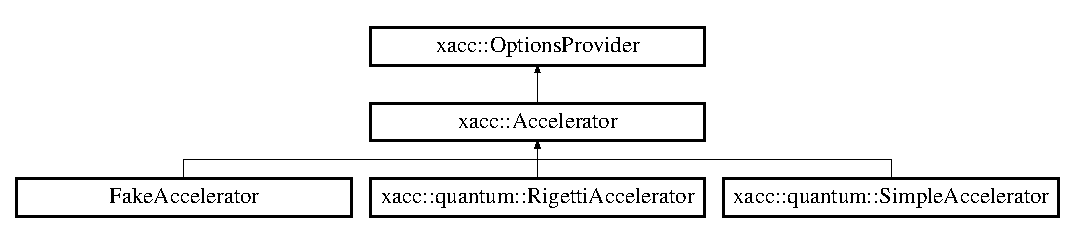
\includegraphics[height=2.679426cm]{a02432}
\end{center}
\end{figure}
\subsection*{Public Member Functions}
\begin{DoxyCompactItemize}
\item 
virtual Accelerator\+Type \hyperlink{a02432_aaffc3e4bb9880eb5041b1b58ee4c2665}{get\+Type} ()=0
\item 
virtual std\+::vector$<$ \hyperlink{a02484}{I\+R\+Transformation} $>$ \hyperlink{a02432_ad6e4a642dcb24e552675bcbeff1e1b04}{get\+I\+R\+Transformations} ()=0
\item 
virtual void \hyperlink{a02432_a89b3f3e6294f228abf03a410b0fb1674}{execute} (std\+::shared\+\_\+ptr$<$ \hyperlink{a02444}{Accelerator\+Buffer} $>$ buffer, const std\+::shared\+\_\+ptr$<$ \hyperlink{a02456}{Function} $>$ function)=0
\item 
virtual std\+::shared\+\_\+ptr$<$ \hyperlink{a02444}{Accelerator\+Buffer} $>$ \hyperlink{a02432_aab5046e8d83ab390302e0f49533e95fc}{create\+Buffer} (const std\+::string \&var\+Id)=0
\item 
virtual std\+::shared\+\_\+ptr$<$ \hyperlink{a02444}{Accelerator\+Buffer} $>$ \hyperlink{a02432_a064a2dbd58338364115c260267806945}{create\+Buffer} (const std\+::string \&var\+Id, const int size)=0
\item 
virtual std\+::shared\+\_\+ptr$<$ \hyperlink{a02444}{Accelerator\+Buffer} $>$ \hyperlink{a02432_ab3820be326e28a553fed1a824f4d41d0}{get\+Buffer} (const std\+::string \&varid)
\item 
virtual bool \hyperlink{a02432_ae51584850faeec77299058383977ddeb}{is\+Valid\+Buffer\+Size} (const int N\+Bits)=0
\item 
virtual std\+::shared\+\_\+ptr$<$ options\+\_\+description $>$ \hyperlink{a02432_a98c9eda6b54367c75667ecfbbf167979}{get\+Options} ()
\item 
virtual \hyperlink{a02432_aed88ab0d71b765f0b0f512684ccd4b55}{$\sim$\+Accelerator} ()
\end{DoxyCompactItemize}
\subsection*{Protected Member Functions}
\begin{DoxyCompactItemize}
\item 
void \hyperlink{a02432_ac3e781f42ec25e460174d4c41ea26b94}{store\+Buffer} (const std\+::string \&id, std\+::shared\+\_\+ptr$<$ \hyperlink{a02444}{Accelerator\+Buffer} $>$ b)
\end{DoxyCompactItemize}


\subsection{Detailed Description}
The \hyperlink{a02432}{Accelerator} class provides a high-\/level abstraction for X\+A\+CC\textquotesingle{}s interaction with attached post-\/exascale accelerators (quantum and neuromorphic processing units).

Derived Accelerators must provide a valid execute implementation that takes X\+A\+CC \hyperlink{a02480}{IR} and executes it on the attached hardware or simulator.

Derived Accelerators must provide a list of \hyperlink{a02484}{I\+R\+Transformation} instances that transform X\+A\+CC \hyperlink{a02480}{IR} to be amenable to execution on the hardware.

Derived Accelerators must provide implementations of create\+Buffer that provide a valid \hyperlink{a02444}{Accelerator\+Buffer} instance modeling the hardware memory or bits being computed on. Upon creating an \hyperlink{a02444}{Accelerator\+Buffer}, derived \hyperlink{a02432}{Accelerator} implementations must call the protected store\+Buffer method to store the \hyperlink{a02444}{Accelerator\+Buffer} for future reference by Compilers and clients of \hyperlink{a02432}{Accelerator}. 

\subsection{Constructor \& Destructor Documentation}
\mbox{\Hypertarget{a02432_aed88ab0d71b765f0b0f512684ccd4b55}\label{a02432_aed88ab0d71b765f0b0f512684ccd4b55}} 
\index{xacc\+::\+Accelerator@{xacc\+::\+Accelerator}!````~Accelerator@{$\sim$\+Accelerator}}
\index{````~Accelerator@{$\sim$\+Accelerator}!xacc\+::\+Accelerator@{xacc\+::\+Accelerator}}
\subsubsection{\texorpdfstring{$\sim$\+Accelerator()}{~Accelerator()}}
{\footnotesize\ttfamily virtual xacc\+::\+Accelerator\+::$\sim$\+Accelerator (\begin{DoxyParamCaption}{ }\end{DoxyParamCaption})\hspace{0.3cm}{\ttfamily [inline]}, {\ttfamily [virtual]}}

Destructor 

\subsection{Member Function Documentation}
\mbox{\Hypertarget{a02432_aab5046e8d83ab390302e0f49533e95fc}\label{a02432_aab5046e8d83ab390302e0f49533e95fc}} 
\index{xacc\+::\+Accelerator@{xacc\+::\+Accelerator}!create\+Buffer@{create\+Buffer}}
\index{create\+Buffer@{create\+Buffer}!xacc\+::\+Accelerator@{xacc\+::\+Accelerator}}
\subsubsection{\texorpdfstring{create\+Buffer()}{createBuffer()}\hspace{0.1cm}{\footnotesize\ttfamily [1/2]}}
{\footnotesize\ttfamily virtual std\+::shared\+\_\+ptr$<$\hyperlink{a02444}{Accelerator\+Buffer}$>$ xacc\+::\+Accelerator\+::create\+Buffer (\begin{DoxyParamCaption}\item[{const std\+::string \&}]{var\+Id }\end{DoxyParamCaption})\hspace{0.3cm}{\ttfamily [pure virtual]}}

Create, store, and return an \hyperlink{a02444}{Accelerator\+Buffer} with the given variable id string. This string serves as a unique identifier for future lookups and reuse of the \hyperlink{a02444}{Accelerator\+Buffer}.


\begin{DoxyParams}{Parameters}
{\em var\+Id} & \\
\hline
\end{DoxyParams}
\begin{DoxyReturn}{Returns}

\end{DoxyReturn}


Implemented in \hyperlink{a01212_ada3ceb986e51ab5aa721f2a08e083cd6}{xacc\+::quantum\+::\+Rigetti\+Accelerator}, \hyperlink{a01244_a46445d77d4b8ad2689571d0db6604380}{xacc\+::quantum\+::\+Simple\+Accelerator}, and \hyperlink{a02496_ae39580fdc83ce9f4df0967382398950e}{Fake\+Accelerator}.

\mbox{\Hypertarget{a02432_a064a2dbd58338364115c260267806945}\label{a02432_a064a2dbd58338364115c260267806945}} 
\index{xacc\+::\+Accelerator@{xacc\+::\+Accelerator}!create\+Buffer@{create\+Buffer}}
\index{create\+Buffer@{create\+Buffer}!xacc\+::\+Accelerator@{xacc\+::\+Accelerator}}
\subsubsection{\texorpdfstring{create\+Buffer()}{createBuffer()}\hspace{0.1cm}{\footnotesize\ttfamily [2/2]}}
{\footnotesize\ttfamily virtual std\+::shared\+\_\+ptr$<$\hyperlink{a02444}{Accelerator\+Buffer}$>$ xacc\+::\+Accelerator\+::create\+Buffer (\begin{DoxyParamCaption}\item[{const std\+::string \&}]{var\+Id,  }\item[{const int}]{size }\end{DoxyParamCaption})\hspace{0.3cm}{\ttfamily [pure virtual]}}

Create, store, and return an \hyperlink{a02444}{Accelerator\+Buffer} with the given variable id string and of the given number of bits. The string id serves as a unique identifier for future lookups and reuse of the \hyperlink{a02444}{Accelerator\+Buffer}.


\begin{DoxyParams}{Parameters}
{\em var\+Id} & \\
\hline
{\em size} & \\
\hline
\end{DoxyParams}
\begin{DoxyReturn}{Returns}

\end{DoxyReturn}


Implemented in \hyperlink{a01212_a731551c94b1abef40d2cf032e8712df6}{xacc\+::quantum\+::\+Rigetti\+Accelerator}, \hyperlink{a01244_adb9393692e9f484df241aa5d014030d1}{xacc\+::quantum\+::\+Simple\+Accelerator}, and \hyperlink{a02496_a09f29b893338dfb0a56dd183cf6949fe}{Fake\+Accelerator}.

\mbox{\Hypertarget{a02432_a89b3f3e6294f228abf03a410b0fb1674}\label{a02432_a89b3f3e6294f228abf03a410b0fb1674}} 
\index{xacc\+::\+Accelerator@{xacc\+::\+Accelerator}!execute@{execute}}
\index{execute@{execute}!xacc\+::\+Accelerator@{xacc\+::\+Accelerator}}
\subsubsection{\texorpdfstring{execute()}{execute()}}
{\footnotesize\ttfamily virtual void xacc\+::\+Accelerator\+::execute (\begin{DoxyParamCaption}\item[{std\+::shared\+\_\+ptr$<$ \hyperlink{a02444}{Accelerator\+Buffer} $>$}]{buffer,  }\item[{const std\+::shared\+\_\+ptr$<$ \hyperlink{a02456}{Function} $>$}]{function }\end{DoxyParamCaption})\hspace{0.3cm}{\ttfamily [pure virtual]}}

Execute the provided X\+A\+CC \hyperlink{a02480}{IR} \hyperlink{a02456}{Function} on the provided \hyperlink{a02444}{Accelerator\+Buffer}.


\begin{DoxyParams}{Parameters}
{\em buffer} & \\
\hline
{\em ir} & \\
\hline
\end{DoxyParams}


Implemented in \hyperlink{a02496_a22c71bda017235865f1b7d4cc5e911fa}{Fake\+Accelerator}.

\mbox{\Hypertarget{a02432_ab3820be326e28a553fed1a824f4d41d0}\label{a02432_ab3820be326e28a553fed1a824f4d41d0}} 
\index{xacc\+::\+Accelerator@{xacc\+::\+Accelerator}!get\+Buffer@{get\+Buffer}}
\index{get\+Buffer@{get\+Buffer}!xacc\+::\+Accelerator@{xacc\+::\+Accelerator}}
\subsubsection{\texorpdfstring{get\+Buffer()}{getBuffer()}}
{\footnotesize\ttfamily virtual std\+::shared\+\_\+ptr$<$\hyperlink{a02444}{Accelerator\+Buffer}$>$ xacc\+::\+Accelerator\+::get\+Buffer (\begin{DoxyParamCaption}\item[{const std\+::string \&}]{varid }\end{DoxyParamCaption})\hspace{0.3cm}{\ttfamily [inline]}, {\ttfamily [virtual]}}

Return the stored \hyperlink{a02444}{Accelerator\+Buffer} with the provided string id.


\begin{DoxyParams}{Parameters}
{\em varid} & \\
\hline
\end{DoxyParams}
\begin{DoxyReturn}{Returns}

\end{DoxyReturn}
\mbox{\Hypertarget{a02432_ad6e4a642dcb24e552675bcbeff1e1b04}\label{a02432_ad6e4a642dcb24e552675bcbeff1e1b04}} 
\index{xacc\+::\+Accelerator@{xacc\+::\+Accelerator}!get\+I\+R\+Transformations@{get\+I\+R\+Transformations}}
\index{get\+I\+R\+Transformations@{get\+I\+R\+Transformations}!xacc\+::\+Accelerator@{xacc\+::\+Accelerator}}
\subsubsection{\texorpdfstring{get\+I\+R\+Transformations()}{getIRTransformations()}}
{\footnotesize\ttfamily virtual std\+::vector$<$\hyperlink{a02484}{I\+R\+Transformation}$>$ xacc\+::\+Accelerator\+::get\+I\+R\+Transformations (\begin{DoxyParamCaption}{ }\end{DoxyParamCaption})\hspace{0.3cm}{\ttfamily [pure virtual]}}

Return any \hyperlink{a02480}{IR} Transformations that must be applied to ensure the compiled \hyperlink{a02480}{IR} is amenable to execution on this \hyperlink{a02432}{Accelerator}. \begin{DoxyReturn}{Returns}

\end{DoxyReturn}


Implemented in \hyperlink{a01212_a443683a1dfb000603c640b2ee303cf66}{xacc\+::quantum\+::\+Rigetti\+Accelerator}, \hyperlink{a01244_afc49c9e7973ba6c6ff9761c36198323d}{xacc\+::quantum\+::\+Simple\+Accelerator}, and \hyperlink{a02496_a6be5485b52606b4543d7e08eda4d6b69}{Fake\+Accelerator}.

\mbox{\Hypertarget{a02432_a98c9eda6b54367c75667ecfbbf167979}\label{a02432_a98c9eda6b54367c75667ecfbbf167979}} 
\index{xacc\+::\+Accelerator@{xacc\+::\+Accelerator}!get\+Options@{get\+Options}}
\index{get\+Options@{get\+Options}!xacc\+::\+Accelerator@{xacc\+::\+Accelerator}}
\subsubsection{\texorpdfstring{get\+Options()}{getOptions()}}
{\footnotesize\ttfamily virtual std\+::shared\+\_\+ptr$<$options\+\_\+description$>$ xacc\+::\+Accelerator\+::get\+Options (\begin{DoxyParamCaption}{ }\end{DoxyParamCaption})\hspace{0.3cm}{\ttfamily [inline]}, {\ttfamily [virtual]}}

Return an empty options\+\_\+description, this is for subclasses to implement. 

Implements \hyperlink{a02536_a6d150954f852109bfe2c1ae90222926f}{xacc\+::\+Options\+Provider}.



Reimplemented in \hyperlink{a01212_a9ee9e62aecbccf193894ca3388676f9f}{xacc\+::quantum\+::\+Rigetti\+Accelerator}.

\mbox{\Hypertarget{a02432_aaffc3e4bb9880eb5041b1b58ee4c2665}\label{a02432_aaffc3e4bb9880eb5041b1b58ee4c2665}} 
\index{xacc\+::\+Accelerator@{xacc\+::\+Accelerator}!get\+Type@{get\+Type}}
\index{get\+Type@{get\+Type}!xacc\+::\+Accelerator@{xacc\+::\+Accelerator}}
\subsubsection{\texorpdfstring{get\+Type()}{getType()}}
{\footnotesize\ttfamily virtual Accelerator\+Type xacc\+::\+Accelerator\+::get\+Type (\begin{DoxyParamCaption}{ }\end{DoxyParamCaption})\hspace{0.3cm}{\ttfamily [pure virtual]}}

Return the type of this \hyperlink{a02432}{Accelerator}.

\begin{DoxyReturn}{Returns}
type The \hyperlink{a02432}{Accelerator} type -\/ Gate or A\+QC Q\+PU, or N\+PU 
\end{DoxyReturn}


Implemented in \hyperlink{a01212_aab0d4674da5273d55407b9ab77cde890}{xacc\+::quantum\+::\+Rigetti\+Accelerator}, \hyperlink{a01244_ad76eeb0bbd7de21aad5bd20d20970a98}{xacc\+::quantum\+::\+Simple\+Accelerator}, and \hyperlink{a02496_abde88dbbf4410bf1c2c3826999e32d47}{Fake\+Accelerator}.

\mbox{\Hypertarget{a02432_ae51584850faeec77299058383977ddeb}\label{a02432_ae51584850faeec77299058383977ddeb}} 
\index{xacc\+::\+Accelerator@{xacc\+::\+Accelerator}!is\+Valid\+Buffer\+Size@{is\+Valid\+Buffer\+Size}}
\index{is\+Valid\+Buffer\+Size@{is\+Valid\+Buffer\+Size}!xacc\+::\+Accelerator@{xacc\+::\+Accelerator}}
\subsubsection{\texorpdfstring{is\+Valid\+Buffer\+Size()}{isValidBufferSize()}}
{\footnotesize\ttfamily virtual bool xacc\+::\+Accelerator\+::is\+Valid\+Buffer\+Size (\begin{DoxyParamCaption}\item[{const int}]{N\+Bits }\end{DoxyParamCaption})\hspace{0.3cm}{\ttfamily [pure virtual]}}

Return true if this \hyperlink{a02432}{Accelerator} can allocated N\+Bits number of bits. 
\begin{DoxyParams}{Parameters}
{\em N\+Bits} & \\
\hline
\end{DoxyParams}
\begin{DoxyReturn}{Returns}

\end{DoxyReturn}


Implemented in \hyperlink{a01212_a61352c07062597aad2393fbeed4cc025}{xacc\+::quantum\+::\+Rigetti\+Accelerator}, \hyperlink{a01244_a60b9db2d6aed235857c45413a070338e}{xacc\+::quantum\+::\+Simple\+Accelerator}, and \hyperlink{a02496_a7a6e63d282dc38fc53c3f3d46ca2ba9b}{Fake\+Accelerator}.

\mbox{\Hypertarget{a02432_ac3e781f42ec25e460174d4c41ea26b94}\label{a02432_ac3e781f42ec25e460174d4c41ea26b94}} 
\index{xacc\+::\+Accelerator@{xacc\+::\+Accelerator}!store\+Buffer@{store\+Buffer}}
\index{store\+Buffer@{store\+Buffer}!xacc\+::\+Accelerator@{xacc\+::\+Accelerator}}
\subsubsection{\texorpdfstring{store\+Buffer()}{storeBuffer()}}
{\footnotesize\ttfamily void xacc\+::\+Accelerator\+::store\+Buffer (\begin{DoxyParamCaption}\item[{const std\+::string \&}]{id,  }\item[{std\+::shared\+\_\+ptr$<$ \hyperlink{a02444}{Accelerator\+Buffer} $>$}]{b }\end{DoxyParamCaption})\hspace{0.3cm}{\ttfamily [inline]}, {\ttfamily [protected]}}

This protected method is to be used by derived Accelerators to store any created \hyperlink{a02444}{Accelerator\+Buffer}.


\begin{DoxyParams}{Parameters}
{\em id} & \\
\hline
{\em b} & \\
\hline
\end{DoxyParams}


The documentation for this class was generated from the following file\+:\begin{DoxyCompactItemize}
\item 
Accelerator.\+hpp\end{DoxyCompactItemize}

\hypertarget{a02440}{}\section{Accelerator\+Bit Class Reference}
\label{a02440}\index{Accelerator\+Bit@{Accelerator\+Bit}}
\subsection*{Public Member Functions}
\begin{DoxyCompactItemize}
\item 
\mbox{\Hypertarget{a02440_a5652247f419d9b749f127b931edcaa80}\label{a02440_a5652247f419d9b749f127b931edcaa80}} 
void {\bfseries update} (int zero\+Or\+One)
\item 
\mbox{\Hypertarget{a02440_aa9cf63ad9c24fedc7519a140a6a6de7f}\label{a02440_aa9cf63ad9c24fedc7519a140a6a6de7f}} 
Accelerator\+Bit\+State {\bfseries get\+State} ()
\end{DoxyCompactItemize}
\subsection*{Protected Attributes}
\begin{DoxyCompactItemize}
\item 
\mbox{\Hypertarget{a02440_a8965d13fb05b41d144a22eceb3bfa85e}\label{a02440_a8965d13fb05b41d144a22eceb3bfa85e}} 
Accelerator\+Bit\+State {\bfseries state}
\end{DoxyCompactItemize}


The documentation for this class was generated from the following file\+:\begin{DoxyCompactItemize}
\item 
Accelerator\+Buffer.\+hpp\end{DoxyCompactItemize}

\hypertarget{a02444}{}\section{Accelerator\+Buffer Class Reference}
\label{a02444}\index{Accelerator\+Buffer@{Accelerator\+Buffer}}


{\ttfamily \#include $<$Accelerator\+Buffer.\+hpp$>$}

Inheritance diagram for Accelerator\+Buffer\+:\begin{figure}[H]
\begin{center}
\leavevmode
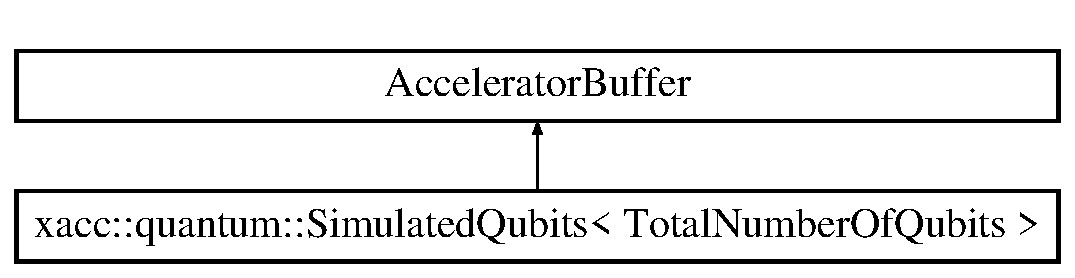
\includegraphics[height=2.000000cm]{a02444}
\end{center}
\end{figure}
\subsection*{Public Member Functions}
\begin{DoxyCompactItemize}
\item 
\mbox{\Hypertarget{a02444_a5115079c3f3f8d32e713f78a91c93a7a}\label{a02444_a5115079c3f3f8d32e713f78a91c93a7a}} 
{\bfseries Accelerator\+Buffer} (const std\+::string \&str)
\item 
\mbox{\Hypertarget{a02444_a6947082735241791c5170d677042da4a}\label{a02444_a6947082735241791c5170d677042da4a}} 
{\bfseries Accelerator\+Buffer} (const std\+::string \&str, const int N)
\item 
\mbox{\Hypertarget{a02444_a96020c3470a86111ae73bdc79ff73237}\label{a02444_a96020c3470a86111ae73bdc79ff73237}} 
{\footnotesize template$<$typename ... Indices$>$ }\\{\bfseries Accelerator\+Buffer} (const std\+::string \&str, int first\+Index, Indices ... indices)
\item 
\mbox{\Hypertarget{a02444_a249eae9f3b83072e5b101ba23f900e81}\label{a02444_a249eae9f3b83072e5b101ba23f900e81}} 
int {\bfseries size} ()
\item 
\mbox{\Hypertarget{a02444_a3373218e4d430d061ba75135bf14ede3}\label{a02444_a3373218e4d430d061ba75135bf14ede3}} 
std\+::string {\bfseries name} ()
\item 
\mbox{\Hypertarget{a02444_aa5080c9a975871858b39d3394e867e77}\label{a02444_aa5080c9a975871858b39d3394e867e77}} 
void {\bfseries reset\+Buffer} ()
\item 
\mbox{\Hypertarget{a02444_a689855524e630049db6120a1493a3c45}\label{a02444_a689855524e630049db6120a1493a3c45}} 
void {\bfseries update\+Bit} (const int idx, int zero\+Or\+One)
\item 
\mbox{\Hypertarget{a02444_a29ece4f7b671308b89c06f3ac8e74b9e}\label{a02444_a29ece4f7b671308b89c06f3ac8e74b9e}} 
Accelerator\+Bit\+State {\bfseries get\+Accelerator\+Bit\+State} (const int idx)
\item 
\mbox{\Hypertarget{a02444_a3776733a3196bca276988d4cc50a135a}\label{a02444_a3776733a3196bca276988d4cc50a135a}} 
virtual void {\bfseries print} ()
\item 
\mbox{\Hypertarget{a02444_a6f2cf905960a528fc829904a3c176c6e}\label{a02444_a6f2cf905960a528fc829904a3c176c6e}} 
virtual void {\bfseries print} (std\+::ostream \&stream)
\end{DoxyCompactItemize}
\subsection*{Protected Attributes}
\begin{DoxyCompactItemize}
\item 
\mbox{\Hypertarget{a02444_adca17dc5025c067a927aefd6a5cbe51b}\label{a02444_adca17dc5025c067a927aefd6a5cbe51b}} 
std\+::string {\bfseries buffer\+Id}
\item 
\mbox{\Hypertarget{a02444_a36b3300cbada4e54e9e68d1c7c135c9b}\label{a02444_a36b3300cbada4e54e9e68d1c7c135c9b}} 
std\+::vector$<$ \hyperlink{a02440}{Accelerator\+Bit} $>$ {\bfseries bits}
\end{DoxyCompactItemize}


\subsection{Detailed Description}
\begin{DoxyAuthor}{Author}
Alex Mc\+Caskey 
\end{DoxyAuthor}


The documentation for this class was generated from the following file\+:\begin{DoxyCompactItemize}
\item 
Accelerator\+Buffer.\+hpp\end{DoxyCompactItemize}

\hypertarget{a01336}{}\section{xacc\+:\+:quantum\+:\+:All\+Gate\+Visitor Class Reference}
\label{a01336}\index{xacc\+::quantum\+::\+All\+Gate\+Visitor@{xacc\+::quantum\+::\+All\+Gate\+Visitor}}


{\ttfamily \#include $<$All\+Gate\+Visitor.\+hpp$>$}

Inheritance diagram for xacc\+:\+:quantum\+:\+:All\+Gate\+Visitor\+:\begin{figure}[H]
\begin{center}
\leavevmode
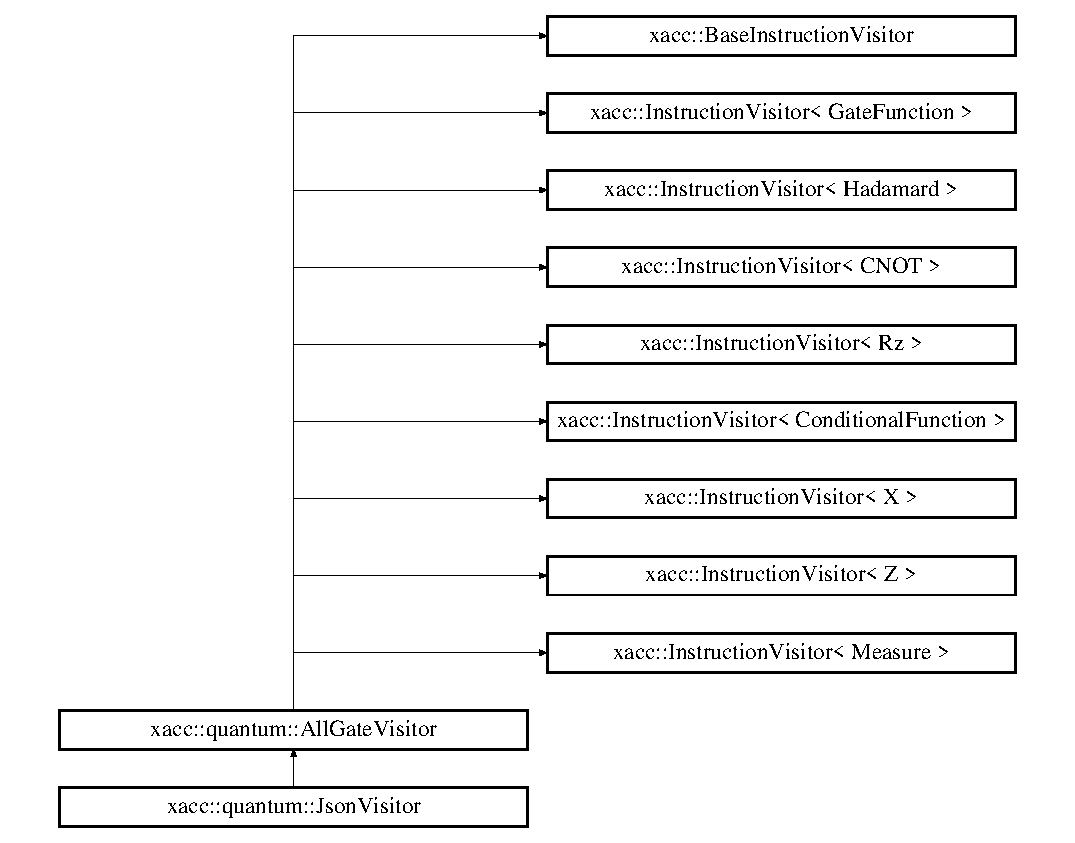
\includegraphics[height=10.883392cm]{a01336}
\end{center}
\end{figure}
\subsection*{Additional Inherited Members}


\subsection{Detailed Description}
F\+I\+X\+ME write this 

The documentation for this class was generated from the following file\+:\begin{DoxyCompactItemize}
\item 
All\+Gate\+Visitor.\+hpp\end{DoxyCompactItemize}

\hypertarget{a02568}{}\section{rapidjson\+:\+:Allocator Class Reference}
\label{a02568}\index{rapidjson\+::\+Allocator@{rapidjson\+::\+Allocator}}


Concept for allocating, resizing and freeing memory block.  




{\ttfamily \#include $<$allocators.\+h$>$}



\subsection{Detailed Description}
Concept for allocating, resizing and freeing memory block. 

Note that Malloc() and Realloc() are non-\/static but Free() is static.

So if an allocator need to support Free(), it needs to put its pointer in the header of memory block.


\begin{DoxyCode}
concept Allocator \{
    \textcolor{keyword}{static} \textcolor{keyword}{const} \textcolor{keywordtype}{bool} kNeedFree;    

    \textcolor{comment}{// Allocate a memory block.}
    \textcolor{comment}{// \(\backslash\)param size of the memory block in bytes.}
    \textcolor{comment}{// \(\backslash\)returns pointer to the memory block.}
    \textcolor{keywordtype}{void}* Malloc(\textcolor{keywordtype}{size\_t} size);

    \textcolor{comment}{// Resize a memory block.}
    \textcolor{comment}{// \(\backslash\)param originalPtr The pointer to current memory block. Null pointer is permitted.}
    \textcolor{comment}{// \(\backslash\)param originalSize The current size in bytes. (Design issue: since some allocator may not book-keep
       this, explicitly pass to it can save memory.)}
    \textcolor{comment}{// \(\backslash\)param newSize the new size in bytes.}
    \textcolor{keywordtype}{void}* Realloc(\textcolor{keywordtype}{void}* originalPtr, \textcolor{keywordtype}{size\_t} originalSize, \textcolor{keywordtype}{size\_t} newSize);

    \textcolor{comment}{// Free a memory block.}
    \textcolor{comment}{// \(\backslash\)param pointer to the memory block. Null pointer is permitted.}
    \textcolor{keyword}{static} \textcolor{keywordtype}{void} Free(\textcolor{keywordtype}{void} *ptr);
\};
\end{DoxyCode}
 

The documentation for this class was generated from the following file\+:\begin{DoxyCompactItemize}
\item 
allocators.\+h\end{DoxyCompactItemize}

\hypertarget{a01828}{}\section{fire\+:\+:array\+\_\+size$<$ T $>$ Struct Template Reference}
\label{a01828}\index{fire\+::array\+\_\+size$<$ T $>$@{fire\+::array\+\_\+size$<$ T $>$}}


{\ttfamily \#include $<$Tensor\+Utils.\+hpp$>$}



\subsection{Detailed Description}
\subsubsection*{template$<$typename T$>$\newline
struct fire\+::array\+\_\+size$<$ T $>$}

This utility template enables the use of std\+::array size integer. 

The documentation for this struct was generated from the following file\+:\begin{DoxyCompactItemize}
\item 
Tensor\+Utils.\+hpp\end{DoxyCompactItemize}

\hypertarget{a01832}{}\section{fire\+:\+:array\+\_\+size$<$ std\+:\+:array$<$ T, N $>$ $>$ Struct Template Reference}
\label{a01832}\index{fire\+::array\+\_\+size$<$ std\+::array$<$ T, N $>$ $>$@{fire\+::array\+\_\+size$<$ std\+::array$<$ T, N $>$ $>$}}
\subsection*{Static Public Attributes}
\begin{DoxyCompactItemize}
\item 
\mbox{\Hypertarget{a01832_ab92887f3c176f5d68d76c67b4db2f112}\label{a01832_ab92887f3c176f5d68d76c67b4db2f112}} 
static const size\+\_\+t {\bfseries value} = N
\end{DoxyCompactItemize}


The documentation for this struct was generated from the following file\+:\begin{DoxyCompactItemize}
\item 
Tensor\+Utils.\+hpp\end{DoxyCompactItemize}

\hypertarget{a02112}{}\section{Generic\+Value$<$ Encoding, Allocator $>$\+:\+:Array\+Data Struct Reference}
\label{a02112}\index{Generic\+Value$<$ Encoding, Allocator $>$\+::\+Array\+Data@{Generic\+Value$<$ Encoding, Allocator $>$\+::\+Array\+Data}}
\subsection*{Public Attributes}
\begin{DoxyCompactItemize}
\item 
\mbox{\Hypertarget{a02112_a5306856f64aea8ec53abf263ed2a35e2}\label{a02112_a5306856f64aea8ec53abf263ed2a35e2}} 
\hyperlink{a00560_a5ed6e6e67250fadbd041127e6386dcb5}{Size\+Type} {\bfseries size}
\item 
\mbox{\Hypertarget{a02112_a0c6fe03c00e13d14b95abd31048aa1f5}\label{a02112_a0c6fe03c00e13d14b95abd31048aa1f5}} 
\hyperlink{a00560_a5ed6e6e67250fadbd041127e6386dcb5}{Size\+Type} {\bfseries capacity}
\item 
\mbox{\Hypertarget{a02112_a86df976cb6f65924aca20eb9bd35553e}\label{a02112_a86df976cb6f65924aca20eb9bd35553e}} 
\hyperlink{a01992}{Generic\+Value} $\ast$ {\bfseries elements}
\end{DoxyCompactItemize}


The documentation for this struct was generated from the following file\+:\begin{DoxyCompactItemize}
\item 
\hyperlink{a00476}{document.\+h}\end{DoxyCompactItemize}



 layout\+: post title\+: Fire Jekyll Configuration permalink\+: /about/jekyll\+\_\+config \subsection*{category\+: about }

Fire uses Jekyll for publishing documentation on Git\+Hub Pages and it uses the \href{http://hemangsk.github.io/Gravity/}{\tt Gravity theme}. There are several important things to keep in mind for this configuration. The Gemfile should contain


\begin{DoxyCode}
source 'https://rubygems.org'

# Ascii Doctor and PlantUML
gem 'jekyll', '~> 2.5'
gem 'asciidoctor', '~> 1.5'
gem 'coderay', '1.1.0'
gem 'rake-jekyll', '~> 1.0'
gem 'jekyll-plantuml', '~> 1.1' 

group :jekyll\_plugins do
  gem "jekyll-asciidoc"
  gem 'asciidoctor-diagram' 
end
\end{DoxyCode}


I ran into two major problems with Git\+Hub that took hours to fix and then only after contacting Git\+Hub directly.


\begin{DoxyItemize}
\item The site.\+url (or just \char`\"{}url\char`\"{}) and site.\+baseurl variables in \+\_\+config.\+yml must be set to \char`\"{}http\+://\mbox{[}username\mbox{]}.\+github.\+io/\mbox{[}project\mbox{]}\char`\"{} for a project level deployment as in
\end{DoxyItemize}


\begin{DoxyCode}
url = "http://jayjaybillings.github.io"
baseurl = "/fire"
\end{DoxyCode}



\begin{DoxyItemize}
\item The only valid places to put github.\+io files are in the master branch, master/docs or in gh-\/pages. I used gh-\/pages/doc and it would not work until I merged into master/docs.
\end{DoxyItemize}

The Gravity theme works as expected when deployed using


\begin{DoxyCode}
bundle exec jekyll serve
\end{DoxyCode}


but deployment to Git\+Hub fails because the style.\+scss file has references to empty scss files in \+\_\+ssas directory starting at line 47. When these imports are removed or commented out, Git\+Hub will build the site.

\subsection*{Acknowledgements }

Thanks to  for encouraging me to not give up and sharing some expertise. Thanks also to Shawna Jean from Git\+Hub for answering my ticket on a Sunday. 
\hypertarget{a01968}{}\section{fire\+:\+:util\+:\+:Asio\+Networking\+Tool$<$ P\+R\+O\+T\+O\+C\+OL $>$ Class Template Reference}
\label{a01968}\index{fire\+::util\+::\+Asio\+Networking\+Tool$<$ P\+R\+O\+T\+O\+C\+O\+L $>$@{fire\+::util\+::\+Asio\+Networking\+Tool$<$ P\+R\+O\+T\+O\+C\+O\+L $>$}}


{\ttfamily \#include $<$Asio\+Networking\+Tool.\+hpp$>$}

Inheritance diagram for fire\+:\+:util\+:\+:Asio\+Networking\+Tool$<$ P\+R\+O\+T\+O\+C\+OL $>$\+:\begin{figure}[H]
\begin{center}
\leavevmode
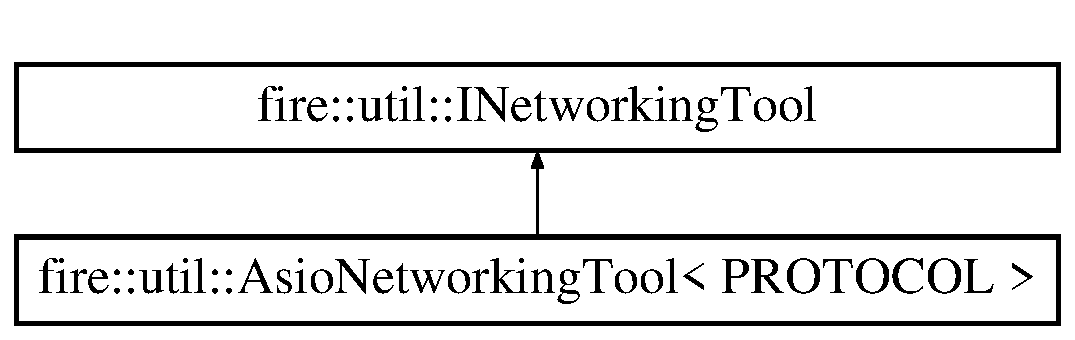
\includegraphics[height=2.000000cm]{a01968}
\end{center}
\end{figure}
\subsection*{Public Member Functions}
\begin{DoxyCompactItemize}
\item 
\hyperlink{a01968_a5edd72ce9937e052a82e7564500b3861}{Asio\+Networking\+Tool} (std\+::string host, int p)
\item 
\mbox{\Hypertarget{a01968_a5826de4a9e051ec854ad7be3a48ac86d}\label{a01968_a5826de4a9e051ec854ad7be3a48ac86d}} 
{\bfseries Asio\+Networking\+Tool} (std\+::string host\+\_\+and\+\_\+port, bool verify\+Cert=true, const std\+::string \&cert\+\_\+file=std\+::string(), const std\+::string \&private\+\_\+key\+\_\+file=std\+::string(), const std\+::string \&verify\+\_\+file=std\+::string())
\item 
virtual \hyperlink{a01968_afc51c728e1bd136b6729ac892df490ab}{$\sim$\+Asio\+Networking\+Tool} ()
\item 
virtual std\+::string \hyperlink{a01968_a40fed691e6b520a8e0f55734466896ca}{get} (const std\+::string \&relative\+Path, const std\+::map$<$ std\+::string, std\+::string $>$ \&header=std\+::map$<$ std\+::string, std\+::string $>$())
\item 
virtual \hyperlink{a01972}{Post\+Response} \hyperlink{a01968_a930b5535c0c68f54d01d4de36cc854a0}{post} (const std\+::string \&relative\+Path, const std\+::string \&message, const std\+::map$<$ std\+::string, std\+::string $>$ \&header=std\+::map$<$ std\+::string, std\+::string $>$())
\item 
std\+::string \hyperlink{a01968_a93d3f6e729eb9980102770f922ca7af4}{base64\+\_\+encode} (char const $\ast$bytes\+\_\+to\+\_\+encode, int in\+\_\+len)
\end{DoxyCompactItemize}
\subsection*{Protected Attributes}
\begin{DoxyCompactItemize}
\item 
std\+::shared\+\_\+ptr$<$ \hyperlink{a01908}{Web\+Client} $>$ \hyperlink{a01968_a57412dca950e86b857ee4795a9b6517e}{client}
\item 
\mbox{\Hypertarget{a01968_a613f571530390cf1d05538c658c13b9e}\label{a01968_a613f571530390cf1d05538c658c13b9e}} 
std\+::shared\+\_\+ptr$<$ Response\+Type $>$ {\bfseries response}
\end{DoxyCompactItemize}


\subsection{Detailed Description}
\subsubsection*{template$<$typename P\+R\+O\+T\+O\+C\+OL$>$\newline
class fire\+::util\+::\+Asio\+Networking\+Tool$<$ P\+R\+O\+T\+O\+C\+O\+L $>$}

The Asio\+Networkign\+Tool is a realization of the \hyperlink{a01976}{I\+Networking\+Tool} interface that uses the B\+O\+O\+ST Asio library to post/get http requests. 

\subsection{Constructor \& Destructor Documentation}
\mbox{\Hypertarget{a01968_a5edd72ce9937e052a82e7564500b3861}\label{a01968_a5edd72ce9937e052a82e7564500b3861}} 
\index{fire\+::util\+::\+Asio\+Networking\+Tool@{fire\+::util\+::\+Asio\+Networking\+Tool}!Asio\+Networking\+Tool@{Asio\+Networking\+Tool}}
\index{Asio\+Networking\+Tool@{Asio\+Networking\+Tool}!fire\+::util\+::\+Asio\+Networking\+Tool@{fire\+::util\+::\+Asio\+Networking\+Tool}}
\subsubsection{\texorpdfstring{Asio\+Networking\+Tool()}{AsioNetworkingTool()}}
{\footnotesize\ttfamily template$<$typename P\+R\+O\+T\+O\+C\+OL $>$ \\
\hyperlink{a01968}{fire\+::util\+::\+Asio\+Networking\+Tool}$<$ P\+R\+O\+T\+O\+C\+OL $>$\+::\hyperlink{a01968}{Asio\+Networking\+Tool} (\begin{DoxyParamCaption}\item[{std\+::string}]{host,  }\item[{int}]{p }\end{DoxyParamCaption})\hspace{0.3cm}{\ttfamily [inline]}}

The constructor \mbox{\Hypertarget{a01968_afc51c728e1bd136b6729ac892df490ab}\label{a01968_afc51c728e1bd136b6729ac892df490ab}} 
\index{fire\+::util\+::\+Asio\+Networking\+Tool@{fire\+::util\+::\+Asio\+Networking\+Tool}!````~Asio\+Networking\+Tool@{$\sim$\+Asio\+Networking\+Tool}}
\index{````~Asio\+Networking\+Tool@{$\sim$\+Asio\+Networking\+Tool}!fire\+::util\+::\+Asio\+Networking\+Tool@{fire\+::util\+::\+Asio\+Networking\+Tool}}
\subsubsection{\texorpdfstring{$\sim$\+Asio\+Networking\+Tool()}{~AsioNetworkingTool()}}
{\footnotesize\ttfamily template$<$typename P\+R\+O\+T\+O\+C\+OL $>$ \\
virtual \hyperlink{a01968}{fire\+::util\+::\+Asio\+Networking\+Tool}$<$ P\+R\+O\+T\+O\+C\+OL $>$\+::$\sim$\hyperlink{a01968}{Asio\+Networking\+Tool} (\begin{DoxyParamCaption}{ }\end{DoxyParamCaption})\hspace{0.3cm}{\ttfamily [inline]}, {\ttfamily [virtual]}}

The destructor 

\subsection{Member Function Documentation}
\mbox{\Hypertarget{a01968_a93d3f6e729eb9980102770f922ca7af4}\label{a01968_a93d3f6e729eb9980102770f922ca7af4}} 
\index{fire\+::util\+::\+Asio\+Networking\+Tool@{fire\+::util\+::\+Asio\+Networking\+Tool}!base64\+\_\+encode@{base64\+\_\+encode}}
\index{base64\+\_\+encode@{base64\+\_\+encode}!fire\+::util\+::\+Asio\+Networking\+Tool@{fire\+::util\+::\+Asio\+Networking\+Tool}}
\subsubsection{\texorpdfstring{base64\+\_\+encode()}{base64\_encode()}}
{\footnotesize\ttfamily template$<$typename P\+R\+O\+T\+O\+C\+OL $>$ \\
std\+::string \hyperlink{a01968}{fire\+::util\+::\+Asio\+Networking\+Tool}$<$ P\+R\+O\+T\+O\+C\+OL $>$\+::base64\+\_\+encode (\begin{DoxyParamCaption}\item[{char const $\ast$}]{bytes\+\_\+to\+\_\+encode,  }\item[{int}]{in\+\_\+len }\end{DoxyParamCaption})\hspace{0.3cm}{\ttfamily [inline]}}


\begin{DoxyParams}{Parameters}
{\em bytes\+\_\+to\+\_\+encode} & \\
\hline
{\em in\+\_\+len} & \\
\hline
\end{DoxyParams}
\begin{DoxyReturn}{Returns}

\end{DoxyReturn}
\mbox{\Hypertarget{a01968_a40fed691e6b520a8e0f55734466896ca}\label{a01968_a40fed691e6b520a8e0f55734466896ca}} 
\index{fire\+::util\+::\+Asio\+Networking\+Tool@{fire\+::util\+::\+Asio\+Networking\+Tool}!get@{get}}
\index{get@{get}!fire\+::util\+::\+Asio\+Networking\+Tool@{fire\+::util\+::\+Asio\+Networking\+Tool}}
\subsubsection{\texorpdfstring{get()}{get()}}
{\footnotesize\ttfamily template$<$typename P\+R\+O\+T\+O\+C\+OL $>$ \\
virtual std\+::string \hyperlink{a01968}{fire\+::util\+::\+Asio\+Networking\+Tool}$<$ P\+R\+O\+T\+O\+C\+OL $>$\+::get (\begin{DoxyParamCaption}\item[{const std\+::string \&}]{relative\+Path,  }\item[{const std\+::map$<$ std\+::string, std\+::string $>$ \&}]{header = {\ttfamily std\+:\+:map$<$~std\+:\+:string,~std\+:\+:string$>$()} }\end{DoxyParamCaption})\hspace{0.3cm}{\ttfamily [inline]}, {\ttfamily [virtual]}}

Return the last received status code.

\begin{DoxyReturn}{Returns}
code The status code as a string Issue an H\+T\+TP G\+ET Command at the given relative path. Clients can provide a map of header key values to modify the G\+ET request.
\end{DoxyReturn}

\begin{DoxyParams}{Parameters}
{\em relative\+Path} & The path relative to the hostname/port provided to this Networking\+Tool \\
\hline
\end{DoxyParams}
\begin{DoxyReturn}{Returns}
The contents at the U\+RL or an error message if one took place. 
\end{DoxyReturn}


Implements \hyperlink{a01976_a58e9426e58cbb9c3b975b9d3e6c1f78f}{fire\+::util\+::\+I\+Networking\+Tool}.

\mbox{\Hypertarget{a01968_a930b5535c0c68f54d01d4de36cc854a0}\label{a01968_a930b5535c0c68f54d01d4de36cc854a0}} 
\index{fire\+::util\+::\+Asio\+Networking\+Tool@{fire\+::util\+::\+Asio\+Networking\+Tool}!post@{post}}
\index{post@{post}!fire\+::util\+::\+Asio\+Networking\+Tool@{fire\+::util\+::\+Asio\+Networking\+Tool}}
\subsubsection{\texorpdfstring{post()}{post()}}
{\footnotesize\ttfamily template$<$typename P\+R\+O\+T\+O\+C\+OL $>$ \\
virtual \hyperlink{a01972}{Post\+Response} \hyperlink{a01968}{fire\+::util\+::\+Asio\+Networking\+Tool}$<$ P\+R\+O\+T\+O\+C\+OL $>$\+::post (\begin{DoxyParamCaption}\item[{const std\+::string \&}]{relative\+Path,  }\item[{const std\+::string \&}]{message,  }\item[{const std\+::map$<$ std\+::string, std\+::string $>$ \&}]{header = {\ttfamily std\+:\+:map$<$~std\+:\+:string,~std\+:\+:string$>$()} }\end{DoxyParamCaption})\hspace{0.3cm}{\ttfamily [inline]}, {\ttfamily [virtual]}}

Issue an H\+T\+TP Post command at the given relative path with the provided message. Clients can provide a map of header key values to modify the P\+O\+ST request.


\begin{DoxyParams}{Parameters}
{\em relative\+Path} & The path relative to the hostname/port provided to this Networking\+Tool \\
\hline
{\em message} & The message to post \\
\hline
{\em header} & The map of additional H\+T\+TP P\+O\+ST header information \\
\hline
\end{DoxyParams}
\begin{DoxyReturn}{Returns}
success Boolean indicating if post was successful 
\end{DoxyReturn}


Implements \hyperlink{a01976_aa585d9b27c43f698203e6c6ec1ee05ce}{fire\+::util\+::\+I\+Networking\+Tool}.



\subsection{Member Data Documentation}
\mbox{\Hypertarget{a01968_a57412dca950e86b857ee4795a9b6517e}\label{a01968_a57412dca950e86b857ee4795a9b6517e}} 
\index{fire\+::util\+::\+Asio\+Networking\+Tool@{fire\+::util\+::\+Asio\+Networking\+Tool}!client@{client}}
\index{client@{client}!fire\+::util\+::\+Asio\+Networking\+Tool@{fire\+::util\+::\+Asio\+Networking\+Tool}}
\subsubsection{\texorpdfstring{client}{client}}
{\footnotesize\ttfamily template$<$typename P\+R\+O\+T\+O\+C\+OL $>$ \\
std\+::shared\+\_\+ptr$<$\hyperlink{a01908}{Web\+Client}$>$ \hyperlink{a01968}{fire\+::util\+::\+Asio\+Networking\+Tool}$<$ P\+R\+O\+T\+O\+C\+OL $>$\+::client\hspace{0.3cm}{\ttfamily [protected]}}

Reference to the asio client we will use 

The documentation for this class was generated from the following file\+:\begin{DoxyCompactItemize}
\item 
Asio\+Networking\+Tool.\+hpp\end{DoxyCompactItemize}

\hypertarget{a02176}{}\section{Auto\+U\+TF$<$ Char\+Type $>$ Struct Template Reference}
\label{a02176}\index{Auto\+U\+T\+F$<$ Char\+Type $>$@{Auto\+U\+T\+F$<$ Char\+Type $>$}}


Dynamically select encoding according to stream\textquotesingle{}s runtime-\/specified U\+TF encoding type.  




{\ttfamily \#include $<$encodings.\+h$>$}

\subsection*{Public Types}
\begin{DoxyCompactItemize}
\item 
\mbox{\Hypertarget{a02176_aacfa2cfd9ad903c9c7110803c4037a7d}\label{a02176_aacfa2cfd9ad903c9c7110803c4037a7d}} 
enum \{ {\bfseries support\+Unicode} = 1
 \}
\item 
\mbox{\Hypertarget{a02176_a0609343de776df3bc31b4c980eb3cf1c}\label{a02176_a0609343de776df3bc31b4c980eb3cf1c}} 
typedef Char\+Type {\bfseries Ch}
\end{DoxyCompactItemize}
\subsection*{Static Public Member Functions}
\begin{DoxyCompactItemize}
\item 
\mbox{\Hypertarget{a02176_a414946115261f886e74dd42cb4b98781}\label{a02176_a414946115261f886e74dd42cb4b98781}} 
{\footnotesize template$<$typename Output\+Stream $>$ }\\static R\+A\+P\+I\+D\+J\+S\+O\+N\+\_\+\+F\+O\+R\+C\+E\+I\+N\+L\+I\+NE void {\bfseries Encode} (Output\+Stream \&os, unsigned codepoint)
\item 
\mbox{\Hypertarget{a02176_a05f5dcd1f153b61b763e44ed452de251}\label{a02176_a05f5dcd1f153b61b763e44ed452de251}} 
{\footnotesize template$<$typename Output\+Stream $>$ }\\static R\+A\+P\+I\+D\+J\+S\+O\+N\+\_\+\+F\+O\+R\+C\+E\+I\+N\+L\+I\+NE void {\bfseries Encode\+Unsafe} (Output\+Stream \&os, unsigned codepoint)
\item 
\mbox{\Hypertarget{a02176_aa5e3c1dc23dbb75f6442ff69500a35b0}\label{a02176_aa5e3c1dc23dbb75f6442ff69500a35b0}} 
{\footnotesize template$<$typename Input\+Stream $>$ }\\static R\+A\+P\+I\+D\+J\+S\+O\+N\+\_\+\+F\+O\+R\+C\+E\+I\+N\+L\+I\+NE bool {\bfseries Decode} (Input\+Stream \&is, unsigned $\ast$codepoint)
\item 
\mbox{\Hypertarget{a02176_a36dd6f226d6a07c12161e21c0aff20b1}\label{a02176_a36dd6f226d6a07c12161e21c0aff20b1}} 
{\footnotesize template$<$typename Input\+Stream , typename Output\+Stream $>$ }\\static R\+A\+P\+I\+D\+J\+S\+O\+N\+\_\+\+F\+O\+R\+C\+E\+I\+N\+L\+I\+NE bool {\bfseries Validate} (Input\+Stream \&is, Output\+Stream \&os)
\end{DoxyCompactItemize}


\subsection{Detailed Description}
\subsubsection*{template$<$typename Char\+Type$>$\newline
struct Auto\+U\+T\+F$<$ Char\+Type $>$}

Dynamically select encoding according to stream\textquotesingle{}s runtime-\/specified U\+TF encoding type. 

\begin{DoxyNote}{Note}
This class can be used with Auto\+U\+T\+F\+Inputt\+Stream and \hyperlink{a02140}{Auto\+U\+T\+F\+Output\+Stream}, which provides Get\+Type(). 
\end{DoxyNote}


The documentation for this struct was generated from the following file\+:\begin{DoxyCompactItemize}
\item 
encodings.\+h\end{DoxyCompactItemize}

\hypertarget{a02136}{}\section{Auto\+U\+T\+F\+Input\+Stream$<$ Char\+Type, Input\+Byte\+Stream $>$ Class Template Reference}
\label{a02136}\index{Auto\+U\+T\+F\+Input\+Stream$<$ Char\+Type, Input\+Byte\+Stream $>$@{Auto\+U\+T\+F\+Input\+Stream$<$ Char\+Type, Input\+Byte\+Stream $>$}}


Input stream wrapper with dynamically bound encoding and automatic encoding detection.  




{\ttfamily \#include $<$encodedstream.\+h$>$}

\subsection*{Public Types}
\begin{DoxyCompactItemize}
\item 
\mbox{\Hypertarget{a02136_a3bb3eb46f2c20404a7ac21963cfe348f}\label{a02136_a3bb3eb46f2c20404a7ac21963cfe348f}} 
typedef Char\+Type {\bfseries Ch}
\end{DoxyCompactItemize}
\subsection*{Public Member Functions}
\begin{DoxyCompactItemize}
\item 
\hyperlink{a02136_a83837fced0971ba26dd9a8ec1575abb0}{Auto\+U\+T\+F\+Input\+Stream} (Input\+Byte\+Stream \&is, U\+T\+F\+Type type=k\+U\+T\+F8)
\begin{DoxyCompactList}\small\item\em Constructor. \end{DoxyCompactList}\item 
\mbox{\Hypertarget{a02136_ad8e8b71e852db11a841fbba40431c5d1}\label{a02136_ad8e8b71e852db11a841fbba40431c5d1}} 
U\+T\+F\+Type {\bfseries Get\+Type} () const
\item 
\mbox{\Hypertarget{a02136_a8831def623c28a3ec1d59b75abe5b20e}\label{a02136_a8831def623c28a3ec1d59b75abe5b20e}} 
bool {\bfseries Has\+B\+OM} () const
\item 
\mbox{\Hypertarget{a02136_a616fbe24878a2026fbc7743acb50438c}\label{a02136_a616fbe24878a2026fbc7743acb50438c}} 
Ch {\bfseries Peek} () const
\item 
\mbox{\Hypertarget{a02136_a652cd1ae8bd848a5ecce4efa1ebd0f38}\label{a02136_a652cd1ae8bd848a5ecce4efa1ebd0f38}} 
Ch {\bfseries Take} ()
\item 
\mbox{\Hypertarget{a02136_a6b847c75309e4ed36957f232b9ce88d1}\label{a02136_a6b847c75309e4ed36957f232b9ce88d1}} 
size\+\_\+t {\bfseries Tell} () const
\item 
\mbox{\Hypertarget{a02136_a5ea730d1ab715f58ce4f9e3dcd77810a}\label{a02136_a5ea730d1ab715f58ce4f9e3dcd77810a}} 
void {\bfseries Put} (Ch)
\item 
\mbox{\Hypertarget{a02136_aecc08f52794d761fc1b729907a83dcf8}\label{a02136_aecc08f52794d761fc1b729907a83dcf8}} 
void {\bfseries Flush} ()
\item 
\mbox{\Hypertarget{a02136_a761841842c147c0bb1a69bfacbc117a2}\label{a02136_a761841842c147c0bb1a69bfacbc117a2}} 
Ch $\ast$ {\bfseries Put\+Begin} ()
\item 
\mbox{\Hypertarget{a02136_a41bd66602f82d344383792feac34f9f7}\label{a02136_a41bd66602f82d344383792feac34f9f7}} 
size\+\_\+t {\bfseries Put\+End} (Ch $\ast$)
\end{DoxyCompactItemize}


\subsection{Detailed Description}
\subsubsection*{template$<$typename Char\+Type, typename Input\+Byte\+Stream$>$\newline
class Auto\+U\+T\+F\+Input\+Stream$<$ Char\+Type, Input\+Byte\+Stream $>$}

Input stream wrapper with dynamically bound encoding and automatic encoding detection. 


\begin{DoxyTemplParams}{Template Parameters}
{\em Char\+Type} & Type of character for reading. \\
\hline
{\em Input\+Byte\+Stream} & type of input byte stream to be wrapped. \\
\hline
\end{DoxyTemplParams}


\subsection{Constructor \& Destructor Documentation}
\mbox{\Hypertarget{a02136_a83837fced0971ba26dd9a8ec1575abb0}\label{a02136_a83837fced0971ba26dd9a8ec1575abb0}} 
\index{Auto\+U\+T\+F\+Input\+Stream@{Auto\+U\+T\+F\+Input\+Stream}!Auto\+U\+T\+F\+Input\+Stream@{Auto\+U\+T\+F\+Input\+Stream}}
\index{Auto\+U\+T\+F\+Input\+Stream@{Auto\+U\+T\+F\+Input\+Stream}!Auto\+U\+T\+F\+Input\+Stream@{Auto\+U\+T\+F\+Input\+Stream}}
\subsubsection{\texorpdfstring{Auto\+U\+T\+F\+Input\+Stream()}{AutoUTFInputStream()}}
{\footnotesize\ttfamily template$<$typename Char\+Type , typename Input\+Byte\+Stream $>$ \\
\hyperlink{a02136}{Auto\+U\+T\+F\+Input\+Stream}$<$ Char\+Type, Input\+Byte\+Stream $>$\+::\hyperlink{a02136}{Auto\+U\+T\+F\+Input\+Stream} (\begin{DoxyParamCaption}\item[{Input\+Byte\+Stream \&}]{is,  }\item[{U\+T\+F\+Type}]{type = {\ttfamily kUTF8} }\end{DoxyParamCaption})\hspace{0.3cm}{\ttfamily [inline]}}



Constructor. 


\begin{DoxyParams}{Parameters}
{\em is} & input stream to be wrapped. \\
\hline
{\em type} & U\+TF encoding type if it is not detected from the stream. \\
\hline
\end{DoxyParams}


The documentation for this class was generated from the following file\+:\begin{DoxyCompactItemize}
\item 
encodedstream.\+h\end{DoxyCompactItemize}

\hypertarget{a02140}{}\section{Auto\+U\+T\+F\+Output\+Stream$<$ Char\+Type, Output\+Byte\+Stream $>$ Class Template Reference}
\label{a02140}\index{Auto\+U\+T\+F\+Output\+Stream$<$ Char\+Type, Output\+Byte\+Stream $>$@{Auto\+U\+T\+F\+Output\+Stream$<$ Char\+Type, Output\+Byte\+Stream $>$}}


Output stream wrapper with dynamically bound encoding and automatic encoding detection.  




{\ttfamily \#include $<$encodedstream.\+h$>$}

\subsection*{Public Types}
\begin{DoxyCompactItemize}
\item 
\mbox{\Hypertarget{a02140_abd8c486101026e11828e86c18991c9c0}\label{a02140_abd8c486101026e11828e86c18991c9c0}} 
typedef Char\+Type {\bfseries Ch}
\end{DoxyCompactItemize}
\subsection*{Public Member Functions}
\begin{DoxyCompactItemize}
\item 
\hyperlink{a02140_a2fe7dbc8e43d11295f66df5653148137}{Auto\+U\+T\+F\+Output\+Stream} (Output\+Byte\+Stream \&os, U\+T\+F\+Type type, bool put\+B\+OM)
\begin{DoxyCompactList}\small\item\em Constructor. \end{DoxyCompactList}\item 
\mbox{\Hypertarget{a02140_a62091565a8103d69002be2e2f4f0ba2c}\label{a02140_a62091565a8103d69002be2e2f4f0ba2c}} 
U\+T\+F\+Type {\bfseries Get\+Type} () const
\item 
\mbox{\Hypertarget{a02140_ad12b33e48c45bdbf2628fd3d5461041a}\label{a02140_ad12b33e48c45bdbf2628fd3d5461041a}} 
void {\bfseries Put} (Ch c)
\item 
\mbox{\Hypertarget{a02140_a38b54c84ba0c479552256ac092529f47}\label{a02140_a38b54c84ba0c479552256ac092529f47}} 
void {\bfseries Flush} ()
\item 
\mbox{\Hypertarget{a02140_ad706f62fd5d22967e5949f3a05087e4e}\label{a02140_ad706f62fd5d22967e5949f3a05087e4e}} 
Ch {\bfseries Peek} () const
\item 
\mbox{\Hypertarget{a02140_a44ee7d84ba13fece17574d01b7be574b}\label{a02140_a44ee7d84ba13fece17574d01b7be574b}} 
Ch {\bfseries Take} ()
\item 
\mbox{\Hypertarget{a02140_a81acbe33d84a28b7d5040d576ae22b5a}\label{a02140_a81acbe33d84a28b7d5040d576ae22b5a}} 
size\+\_\+t {\bfseries Tell} () const
\item 
\mbox{\Hypertarget{a02140_a3c7333661dba3d2210f0b287bdd6c1f3}\label{a02140_a3c7333661dba3d2210f0b287bdd6c1f3}} 
Ch $\ast$ {\bfseries Put\+Begin} ()
\item 
\mbox{\Hypertarget{a02140_a4b16bda191526c894501fce447e95b8d}\label{a02140_a4b16bda191526c894501fce447e95b8d}} 
size\+\_\+t {\bfseries Put\+End} (Ch $\ast$)
\end{DoxyCompactItemize}


\subsection{Detailed Description}
\subsubsection*{template$<$typename Char\+Type, typename Output\+Byte\+Stream$>$\newline
class Auto\+U\+T\+F\+Output\+Stream$<$ Char\+Type, Output\+Byte\+Stream $>$}

Output stream wrapper with dynamically bound encoding and automatic encoding detection. 


\begin{DoxyTemplParams}{Template Parameters}
{\em Char\+Type} & Type of character for writing. \\
\hline
{\em Output\+Byte\+Stream} & type of output byte stream to be wrapped. \\
\hline
\end{DoxyTemplParams}


\subsection{Constructor \& Destructor Documentation}
\mbox{\Hypertarget{a02140_a2fe7dbc8e43d11295f66df5653148137}\label{a02140_a2fe7dbc8e43d11295f66df5653148137}} 
\index{Auto\+U\+T\+F\+Output\+Stream@{Auto\+U\+T\+F\+Output\+Stream}!Auto\+U\+T\+F\+Output\+Stream@{Auto\+U\+T\+F\+Output\+Stream}}
\index{Auto\+U\+T\+F\+Output\+Stream@{Auto\+U\+T\+F\+Output\+Stream}!Auto\+U\+T\+F\+Output\+Stream@{Auto\+U\+T\+F\+Output\+Stream}}
\subsubsection{\texorpdfstring{Auto\+U\+T\+F\+Output\+Stream()}{AutoUTFOutputStream()}}
{\footnotesize\ttfamily template$<$typename Char\+Type , typename Output\+Byte\+Stream $>$ \\
\hyperlink{a02140}{Auto\+U\+T\+F\+Output\+Stream}$<$ Char\+Type, Output\+Byte\+Stream $>$\+::\hyperlink{a02140}{Auto\+U\+T\+F\+Output\+Stream} (\begin{DoxyParamCaption}\item[{Output\+Byte\+Stream \&}]{os,  }\item[{U\+T\+F\+Type}]{type,  }\item[{bool}]{put\+B\+OM }\end{DoxyParamCaption})\hspace{0.3cm}{\ttfamily [inline]}}



Constructor. 


\begin{DoxyParams}{Parameters}
{\em os} & output stream to be wrapped. \\
\hline
{\em type} & U\+TF encoding type. \\
\hline
{\em put\+B\+OM} & Whether to write B\+OM at the beginning of the stream. \\
\hline
\end{DoxyParams}


The documentation for this class was generated from the following file\+:\begin{DoxyCompactItemize}
\item 
encodedstream.\+h\end{DoxyCompactItemize}

\hypertarget{a02476}{}\section{xacc\+:\+:Base\+Instruction\+Visitable Class Reference}
\label{a02476}\index{xacc\+::\+Base\+Instruction\+Visitable@{xacc\+::\+Base\+Instruction\+Visitable}}


{\ttfamily \#include $<$Instruction\+Visitor.\+hpp$>$}

Inheritance diagram for xacc\+:\+:Base\+Instruction\+Visitable\+:\begin{figure}[H]
\begin{center}
\leavevmode
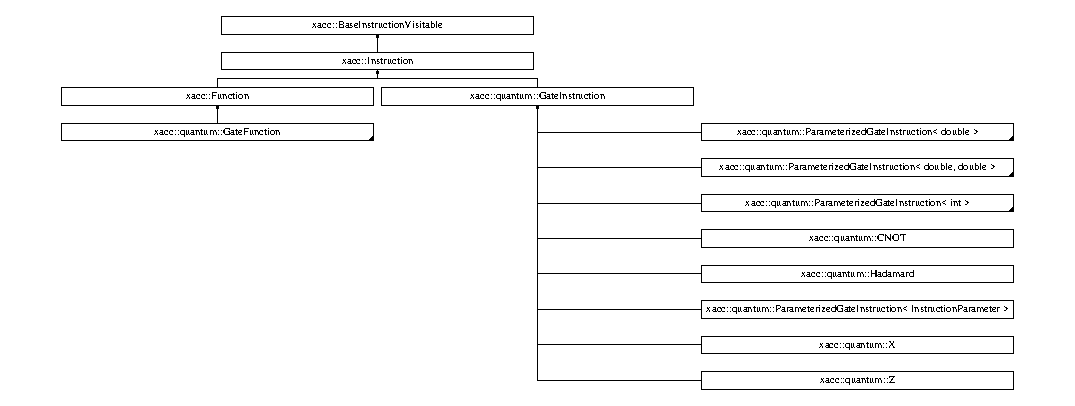
\includegraphics[height=5.008130cm]{a02476}
\end{center}
\end{figure}
\subsection*{Public Member Functions}
\begin{DoxyCompactItemize}
\item 
virtual void \hyperlink{a02476_a4ae295a7f83d57c6f1f912adc90274ea}{accept} (std\+::shared\+\_\+ptr$<$ \hyperlink{a02468}{Base\+Instruction\+Visitor} $>$ visitor)=0
\item 
virtual void \hyperlink{a02476_ad6b9ad95c14580cc86ca87cd464262c3}{accept} (\hyperlink{a02468}{Base\+Instruction\+Visitor} $\ast$visitor)=0
\item 
virtual \hyperlink{a02476_a3a291d247b18ea7620dd8d97dfb595f4}{$\sim$\+Base\+Instruction\+Visitable} ()
\end{DoxyCompactItemize}
\subsection*{Static Protected Member Functions}
\begin{DoxyCompactItemize}
\item 
{\footnotesize template$<$class T $>$ }\\static void \hyperlink{a02476_a2f18b9fcb48f42d190a9f5180b7b59c5}{accept\+Impl} (T \&visited, std\+::shared\+\_\+ptr$<$ \hyperlink{a02468}{Base\+Instruction\+Visitor} $>$ visitor)
\item 
{\footnotesize template$<$class T $>$ }\\static void \hyperlink{a02476_a80c7bb995faa54644f822fa48176c6cb}{accept\+Impl} (T \&visited, \hyperlink{a02468}{Base\+Instruction\+Visitor} $\ast$visitor)
\end{DoxyCompactItemize}


\subsection{Detailed Description}
\hyperlink{a02476}{Base\+Instruction\+Visitable} is an interface that is to be implemented by any and all Instructions that want to be available for visitation. Derivations of this class simply inherit from \hyperlink{a02476}{Base\+Instruction\+Visitable} and declare the D\+E\+F\+I\+N\+E\+\_\+\+V\+I\+S\+I\+T\+A\+B\+LE macro alongside the rest of the classes member methods. 

\subsection{Constructor \& Destructor Documentation}
\mbox{\Hypertarget{a02476_a3a291d247b18ea7620dd8d97dfb595f4}\label{a02476_a3a291d247b18ea7620dd8d97dfb595f4}} 
\index{xacc\+::\+Base\+Instruction\+Visitable@{xacc\+::\+Base\+Instruction\+Visitable}!````~Base\+Instruction\+Visitable@{$\sim$\+Base\+Instruction\+Visitable}}
\index{````~Base\+Instruction\+Visitable@{$\sim$\+Base\+Instruction\+Visitable}!xacc\+::\+Base\+Instruction\+Visitable@{xacc\+::\+Base\+Instruction\+Visitable}}
\subsubsection{\texorpdfstring{$\sim$\+Base\+Instruction\+Visitable()}{~BaseInstructionVisitable()}}
{\footnotesize\ttfamily virtual xacc\+::\+Base\+Instruction\+Visitable\+::$\sim$\+Base\+Instruction\+Visitable (\begin{DoxyParamCaption}{ }\end{DoxyParamCaption})\hspace{0.3cm}{\ttfamily [inline]}, {\ttfamily [virtual]}}

The Destructor 

\subsection{Member Function Documentation}
\mbox{\Hypertarget{a02476_a4ae295a7f83d57c6f1f912adc90274ea}\label{a02476_a4ae295a7f83d57c6f1f912adc90274ea}} 
\index{xacc\+::\+Base\+Instruction\+Visitable@{xacc\+::\+Base\+Instruction\+Visitable}!accept@{accept}}
\index{accept@{accept}!xacc\+::\+Base\+Instruction\+Visitable@{xacc\+::\+Base\+Instruction\+Visitable}}
\subsubsection{\texorpdfstring{accept()}{accept()}\hspace{0.1cm}{\footnotesize\ttfamily [1/2]}}
{\footnotesize\ttfamily virtual void xacc\+::\+Base\+Instruction\+Visitable\+::accept (\begin{DoxyParamCaption}\item[{std\+::shared\+\_\+ptr$<$ \hyperlink{a02468}{Base\+Instruction\+Visitor} $>$}]{visitor }\end{DoxyParamCaption})\hspace{0.3cm}{\ttfamily [pure virtual]}}

Accept the provided \hyperlink{a02468}{Base\+Instruction\+Visitor} as a shared pointer. 
\begin{DoxyParams}{Parameters}
{\em visitor} & The visitor to invoke visit() on. \\
\hline
\end{DoxyParams}
\mbox{\Hypertarget{a02476_ad6b9ad95c14580cc86ca87cd464262c3}\label{a02476_ad6b9ad95c14580cc86ca87cd464262c3}} 
\index{xacc\+::\+Base\+Instruction\+Visitable@{xacc\+::\+Base\+Instruction\+Visitable}!accept@{accept}}
\index{accept@{accept}!xacc\+::\+Base\+Instruction\+Visitable@{xacc\+::\+Base\+Instruction\+Visitable}}
\subsubsection{\texorpdfstring{accept()}{accept()}\hspace{0.1cm}{\footnotesize\ttfamily [2/2]}}
{\footnotesize\ttfamily virtual void xacc\+::\+Base\+Instruction\+Visitable\+::accept (\begin{DoxyParamCaption}\item[{\hyperlink{a02468}{Base\+Instruction\+Visitor} $\ast$}]{visitor }\end{DoxyParamCaption})\hspace{0.3cm}{\ttfamily [pure virtual]}}

Accept the provided \hyperlink{a02468}{Base\+Instruction\+Visitor} as a raw pointer. 
\begin{DoxyParams}{Parameters}
{\em visitor} & The visitor to invoke visit() on. \\
\hline
\end{DoxyParams}
\mbox{\Hypertarget{a02476_a2f18b9fcb48f42d190a9f5180b7b59c5}\label{a02476_a2f18b9fcb48f42d190a9f5180b7b59c5}} 
\index{xacc\+::\+Base\+Instruction\+Visitable@{xacc\+::\+Base\+Instruction\+Visitable}!accept\+Impl@{accept\+Impl}}
\index{accept\+Impl@{accept\+Impl}!xacc\+::\+Base\+Instruction\+Visitable@{xacc\+::\+Base\+Instruction\+Visitable}}
\subsubsection{\texorpdfstring{accept\+Impl()}{acceptImpl()}\hspace{0.1cm}{\footnotesize\ttfamily [1/2]}}
{\footnotesize\ttfamily template$<$class T $>$ \\
static void xacc\+::\+Base\+Instruction\+Visitable\+::accept\+Impl (\begin{DoxyParamCaption}\item[{T \&}]{visited,  }\item[{std\+::shared\+\_\+ptr$<$ \hyperlink{a02468}{Base\+Instruction\+Visitor} $>$}]{visitor }\end{DoxyParamCaption})\hspace{0.3cm}{\ttfamily [inline]}, {\ttfamily [static]}, {\ttfamily [protected]}}

This method is invoked by the D\+E\+F\+I\+N\+E\+\_\+\+V\+I\+S\+I\+T\+A\+B\+LE macro to invoke the visit method on the provided visitor. This method takes the visitor as a shared pointer. \mbox{\Hypertarget{a02476_a80c7bb995faa54644f822fa48176c6cb}\label{a02476_a80c7bb995faa54644f822fa48176c6cb}} 
\index{xacc\+::\+Base\+Instruction\+Visitable@{xacc\+::\+Base\+Instruction\+Visitable}!accept\+Impl@{accept\+Impl}}
\index{accept\+Impl@{accept\+Impl}!xacc\+::\+Base\+Instruction\+Visitable@{xacc\+::\+Base\+Instruction\+Visitable}}
\subsubsection{\texorpdfstring{accept\+Impl()}{acceptImpl()}\hspace{0.1cm}{\footnotesize\ttfamily [2/2]}}
{\footnotesize\ttfamily template$<$class T $>$ \\
static void xacc\+::\+Base\+Instruction\+Visitable\+::accept\+Impl (\begin{DoxyParamCaption}\item[{T \&}]{visited,  }\item[{\hyperlink{a02468}{Base\+Instruction\+Visitor} $\ast$}]{visitor }\end{DoxyParamCaption})\hspace{0.3cm}{\ttfamily [inline]}, {\ttfamily [static]}, {\ttfamily [protected]}}

This method is invoked by the D\+E\+F\+I\+N\+E\+\_\+\+V\+I\+S\+I\+T\+A\+B\+LE macro to invoke the visit method on the provided visitor. This method takes the visitor as a raw pointer. 

The documentation for this class was generated from the following file\+:\begin{DoxyCompactItemize}
\item 
Instruction\+Visitor.\+hpp\end{DoxyCompactItemize}

\hypertarget{a02468}{}\section{xacc\+:\+:Base\+Instruction\+Visitor Class Reference}
\label{a02468}\index{xacc\+::\+Base\+Instruction\+Visitor@{xacc\+::\+Base\+Instruction\+Visitor}}


{\ttfamily \#include $<$Instruction\+Visitor.\+hpp$>$}

Inheritance diagram for xacc\+:\+:Base\+Instruction\+Visitor\+:\begin{figure}[H]
\begin{center}
\leavevmode
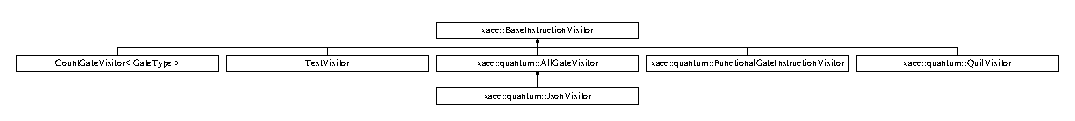
\includegraphics[height=1.183099cm]{a02468}
\end{center}
\end{figure}
\subsection*{Public Member Functions}
\begin{DoxyCompactItemize}
\item 
virtual \hyperlink{a02468_aa6f5104f5868fe1eca9be4dc4036eba4}{$\sim$\+Base\+Instruction\+Visitor} ()
\end{DoxyCompactItemize}


\subsection{Detailed Description}
The \hyperlink{a02468}{Base\+Instruction\+Visitor} is a base class for all classes that are \hyperlink{a02460}{Instruction} visitors. It basically provides a means for passing instruction visitor handles in a polymorphic manner. 

\subsection{Constructor \& Destructor Documentation}
\mbox{\Hypertarget{a02468_aa6f5104f5868fe1eca9be4dc4036eba4}\label{a02468_aa6f5104f5868fe1eca9be4dc4036eba4}} 
\index{xacc\+::\+Base\+Instruction\+Visitor@{xacc\+::\+Base\+Instruction\+Visitor}!````~Base\+Instruction\+Visitor@{$\sim$\+Base\+Instruction\+Visitor}}
\index{````~Base\+Instruction\+Visitor@{$\sim$\+Base\+Instruction\+Visitor}!xacc\+::\+Base\+Instruction\+Visitor@{xacc\+::\+Base\+Instruction\+Visitor}}
\subsubsection{\texorpdfstring{$\sim$\+Base\+Instruction\+Visitor()}{~BaseInstructionVisitor()}}
{\footnotesize\ttfamily virtual xacc\+::\+Base\+Instruction\+Visitor\+::$\sim$\+Base\+Instruction\+Visitor (\begin{DoxyParamCaption}{ }\end{DoxyParamCaption})\hspace{0.3cm}{\ttfamily [inline]}, {\ttfamily [virtual]}}

The destructor 

The documentation for this class was generated from the following file\+:\begin{DoxyCompactItemize}
\item 
Instruction\+Visitor.\+hpp\end{DoxyCompactItemize}

\hypertarget{a02216}{}\section{Base\+Reader\+Handler$<$ Encoding, Derived $>$ Struct Template Reference}
\label{a02216}\index{Base\+Reader\+Handler$<$ Encoding, Derived $>$@{Base\+Reader\+Handler$<$ Encoding, Derived $>$}}


Default implementation of Handler.  




{\ttfamily \#include $<$reader.\+h$>$}

\subsection*{Public Types}
\begin{DoxyCompactItemize}
\item 
\mbox{\Hypertarget{a02216_a8302c755dd3560c8c5bac99162c28214}\label{a02216_a8302c755dd3560c8c5bac99162c28214}} 
typedef Encoding\+::\+Ch {\bfseries Ch}
\item 
\mbox{\Hypertarget{a02216_a7b6c70d9bf7483b2de5d249f1593776a}\label{a02216_a7b6c70d9bf7483b2de5d249f1593776a}} 
typedef internal\+::\+Select\+If$<$ internal\+::\+Is\+Same$<$ Derived, void $>$, \hyperlink{a02216}{Base\+Reader\+Handler}, Derived $>$\+::\hyperlink{a00560_a1d1cfd8ffb84e947f82999c682b666a7}{Type} {\bfseries Override}
\end{DoxyCompactItemize}
\subsection*{Public Member Functions}
\begin{DoxyCompactItemize}
\item 
\mbox{\Hypertarget{a02216_a836437f6ccc37f08ff933f009b18a78c}\label{a02216_a836437f6ccc37f08ff933f009b18a78c}} 
bool {\bfseries Default} ()
\item 
\mbox{\Hypertarget{a02216_ae2ebbde4628bf3659ddc5d18520935f5}\label{a02216_ae2ebbde4628bf3659ddc5d18520935f5}} 
bool {\bfseries Null} ()
\item 
\mbox{\Hypertarget{a02216_aa1c3ce42dbb856b3349792dc9d963587}\label{a02216_aa1c3ce42dbb856b3349792dc9d963587}} 
bool {\bfseries Bool} (bool)
\item 
\mbox{\Hypertarget{a02216_a85e813aaf7189a2f87bd53953324fafc}\label{a02216_a85e813aaf7189a2f87bd53953324fafc}} 
bool {\bfseries Int} (int)
\item 
\mbox{\Hypertarget{a02216_a0e683306cbb7b4e350a35c18c5246f2a}\label{a02216_a0e683306cbb7b4e350a35c18c5246f2a}} 
bool {\bfseries Uint} (unsigned)
\item 
\mbox{\Hypertarget{a02216_a04011733ea584739c97ad5c6afa15a35}\label{a02216_a04011733ea584739c97ad5c6afa15a35}} 
bool {\bfseries Int64} (int64\+\_\+t)
\item 
\mbox{\Hypertarget{a02216_a351aa3cd81856a487c21022e9cc64d2b}\label{a02216_a351aa3cd81856a487c21022e9cc64d2b}} 
bool {\bfseries Uint64} (uint64\+\_\+t)
\item 
\mbox{\Hypertarget{a02216_a8156ea6ae5b8cd23a8b700e92a8af1eb}\label{a02216_a8156ea6ae5b8cd23a8b700e92a8af1eb}} 
bool {\bfseries Double} (double)
\item 
\mbox{\Hypertarget{a02216_a9ed0d83d5e6c8f5e4b32ca3735ff0bb7}\label{a02216_a9ed0d83d5e6c8f5e4b32ca3735ff0bb7}} 
bool \hyperlink{a02216_a9ed0d83d5e6c8f5e4b32ca3735ff0bb7}{Raw\+Number} (const Ch $\ast$str, \hyperlink{a00560_a5ed6e6e67250fadbd041127e6386dcb5}{Size\+Type} len, bool copy)
\begin{DoxyCompactList}\small\item\em enabled via k\+Parse\+Numbers\+As\+Strings\+Flag, string is not null-\/terminated (use length) \end{DoxyCompactList}\item 
\mbox{\Hypertarget{a02216_a3ac69e6326d0aeef7b1f2619742bbe00}\label{a02216_a3ac69e6326d0aeef7b1f2619742bbe00}} 
bool {\bfseries String} (const Ch $\ast$, \hyperlink{a00560_a5ed6e6e67250fadbd041127e6386dcb5}{Size\+Type}, bool)
\item 
\mbox{\Hypertarget{a02216_ab0a7d9bcececb8d6ed748656f67f4917}\label{a02216_ab0a7d9bcececb8d6ed748656f67f4917}} 
bool {\bfseries Start\+Object} ()
\item 
\mbox{\Hypertarget{a02216_abc50b2e7e411b7b731715e05cd01e2eb}\label{a02216_abc50b2e7e411b7b731715e05cd01e2eb}} 
bool {\bfseries Key} (const Ch $\ast$str, \hyperlink{a00560_a5ed6e6e67250fadbd041127e6386dcb5}{Size\+Type} len, bool copy)
\item 
\mbox{\Hypertarget{a02216_a0406cee0af26bc3a0b7fb2414537b0ab}\label{a02216_a0406cee0af26bc3a0b7fb2414537b0ab}} 
bool {\bfseries End\+Object} (\hyperlink{a00560_a5ed6e6e67250fadbd041127e6386dcb5}{Size\+Type})
\item 
\mbox{\Hypertarget{a02216_a9dbb1143a250a904bb18a174553a3a00}\label{a02216_a9dbb1143a250a904bb18a174553a3a00}} 
bool {\bfseries Start\+Array} ()
\item 
\mbox{\Hypertarget{a02216_ae9d60a8779b6a77a7f283d64961879fb}\label{a02216_ae9d60a8779b6a77a7f283d64961879fb}} 
bool {\bfseries End\+Array} (\hyperlink{a00560_a5ed6e6e67250fadbd041127e6386dcb5}{Size\+Type})
\end{DoxyCompactItemize}


\subsection{Detailed Description}
\subsubsection*{template$<$typename Encoding = U\+T\+F8$<$$>$, typename Derived = void$>$\newline
struct Base\+Reader\+Handler$<$ Encoding, Derived $>$}

Default implementation of Handler. 

This can be used as base class of any reader handler. \begin{DoxyNote}{Note}
implements Handler concept 
\end{DoxyNote}


The documentation for this struct was generated from the following files\+:\begin{DoxyCompactItemize}
\item 
fwd.\+h\item 
\hyperlink{a00563}{reader.\+h}\end{DoxyCompactItemize}

\hypertarget{a02292}{}\section{Basic\+I\+Stream\+Wrapper$<$ Stream\+Type $>$ Class Template Reference}
\label{a02292}\index{Basic\+I\+Stream\+Wrapper$<$ Stream\+Type $>$@{Basic\+I\+Stream\+Wrapper$<$ Stream\+Type $>$}}


Wrapper of {\ttfamily std\+::basic\+\_\+istream} into Rapid\+J\+S\+ON\textquotesingle{}s Stream concept.  




{\ttfamily \#include $<$istreamwrapper.\+h$>$}

\subsection*{Public Types}
\begin{DoxyCompactItemize}
\item 
\mbox{\Hypertarget{a02292_a88e4288ecdaa0d31ddf4e5917b9aa8d7}\label{a02292_a88e4288ecdaa0d31ddf4e5917b9aa8d7}} 
typedef Stream\+Type\+::char\+\_\+type {\bfseries Ch}
\end{DoxyCompactItemize}
\subsection*{Public Member Functions}
\begin{DoxyCompactItemize}
\item 
\mbox{\Hypertarget{a02292_a3e9a2dd2b6b28243f8f2a911f67cdf56}\label{a02292_a3e9a2dd2b6b28243f8f2a911f67cdf56}} 
{\bfseries Basic\+I\+Stream\+Wrapper} (Stream\+Type \&stream)
\item 
\mbox{\Hypertarget{a02292_a0ad1488235b4786dd4f7a16e679dec88}\label{a02292_a0ad1488235b4786dd4f7a16e679dec88}} 
Ch {\bfseries Peek} () const
\item 
\mbox{\Hypertarget{a02292_afb71f0329d0abbbc9b22ebeb5c1464d1}\label{a02292_afb71f0329d0abbbc9b22ebeb5c1464d1}} 
Ch {\bfseries Take} ()
\item 
\mbox{\Hypertarget{a02292_ac212848265f937add49bd973de794e25}\label{a02292_ac212848265f937add49bd973de794e25}} 
size\+\_\+t {\bfseries Tell} () const
\item 
\mbox{\Hypertarget{a02292_a62a3fc10b009ea231fb9d2dc958c539c}\label{a02292_a62a3fc10b009ea231fb9d2dc958c539c}} 
Ch $\ast$ {\bfseries Put\+Begin} ()
\item 
\mbox{\Hypertarget{a02292_afa71cb2f5b7668837d0a81e3bce55e69}\label{a02292_afa71cb2f5b7668837d0a81e3bce55e69}} 
void {\bfseries Put} (Ch)
\item 
\mbox{\Hypertarget{a02292_a37d5e4cd8fdf3c83dad50737e95886a9}\label{a02292_a37d5e4cd8fdf3c83dad50737e95886a9}} 
void {\bfseries Flush} ()
\item 
\mbox{\Hypertarget{a02292_ab2ead53490207a1cb0bdd674a03957f3}\label{a02292_ab2ead53490207a1cb0bdd674a03957f3}} 
size\+\_\+t {\bfseries Put\+End} (Ch $\ast$)
\item 
\mbox{\Hypertarget{a02292_ae8b52683adc67ca0b91484a427aed660}\label{a02292_ae8b52683adc67ca0b91484a427aed660}} 
const Ch $\ast$ {\bfseries Peek4} () const
\end{DoxyCompactItemize}


\subsection{Detailed Description}
\subsubsection*{template$<$typename Stream\+Type$>$\newline
class Basic\+I\+Stream\+Wrapper$<$ Stream\+Type $>$}

Wrapper of {\ttfamily std\+::basic\+\_\+istream} into Rapid\+J\+S\+ON\textquotesingle{}s Stream concept. 

The classes can be wrapped including but not limited to\+:


\begin{DoxyItemize}
\item {\ttfamily std\+::istringstream} 
\item {\ttfamily std\+::stringstream} 
\item {\ttfamily std\+::wistringstream} 
\item {\ttfamily std\+::wstringstream} 
\item {\ttfamily std\+::ifstream} 
\item {\ttfamily std\+::fstream} 
\item {\ttfamily std\+::wifstream} 
\item {\ttfamily std\+::wfstream} 
\end{DoxyItemize}


\begin{DoxyTemplParams}{Template Parameters}
{\em Stream\+Type} & Class derived from {\ttfamily std\+::basic\+\_\+istream}. \\
\hline
\end{DoxyTemplParams}


The documentation for this class was generated from the following file\+:\begin{DoxyCompactItemize}
\item 
istreamwrapper.\+h\end{DoxyCompactItemize}

\hypertarget{a02304}{}\section{Basic\+O\+Stream\+Wrapper$<$ Stream\+Type $>$ Class Template Reference}
\label{a02304}\index{Basic\+O\+Stream\+Wrapper$<$ Stream\+Type $>$@{Basic\+O\+Stream\+Wrapper$<$ Stream\+Type $>$}}


Wrapper of {\ttfamily std\+::basic\+\_\+ostream} into Rapid\+J\+S\+ON\textquotesingle{}s Stream concept.  




{\ttfamily \#include $<$ostreamwrapper.\+h$>$}

\subsection*{Public Types}
\begin{DoxyCompactItemize}
\item 
\mbox{\Hypertarget{a02304_aafc6276f1f5cc0b8d45d137584d380bb}\label{a02304_aafc6276f1f5cc0b8d45d137584d380bb}} 
typedef Stream\+Type\+::char\+\_\+type {\bfseries Ch}
\end{DoxyCompactItemize}
\subsection*{Public Member Functions}
\begin{DoxyCompactItemize}
\item 
\mbox{\Hypertarget{a02304_a067a516c13b7c9d4dacef598d32779ef}\label{a02304_a067a516c13b7c9d4dacef598d32779ef}} 
{\bfseries Basic\+O\+Stream\+Wrapper} (Stream\+Type \&stream)
\item 
\mbox{\Hypertarget{a02304_a7d3ba9d651fbe27fe05387f512154ea8}\label{a02304_a7d3ba9d651fbe27fe05387f512154ea8}} 
void {\bfseries Put} (Ch c)
\item 
\mbox{\Hypertarget{a02304_a1c48a8b7520b0ab6ca34e665b928b56d}\label{a02304_a1c48a8b7520b0ab6ca34e665b928b56d}} 
void {\bfseries Flush} ()
\item 
\mbox{\Hypertarget{a02304_a6dc18ded82487d41a2d123e21a9e050b}\label{a02304_a6dc18ded82487d41a2d123e21a9e050b}} 
char {\bfseries Peek} () const
\item 
\mbox{\Hypertarget{a02304_a54be63e8d24f4d82329b860a907f65fe}\label{a02304_a54be63e8d24f4d82329b860a907f65fe}} 
char {\bfseries Take} ()
\item 
\mbox{\Hypertarget{a02304_a62f214649fbfb8380a69fe92b864a61b}\label{a02304_a62f214649fbfb8380a69fe92b864a61b}} 
size\+\_\+t {\bfseries Tell} () const
\item 
\mbox{\Hypertarget{a02304_a564b7b727bdab12185e7a7bd1ac5e822}\label{a02304_a564b7b727bdab12185e7a7bd1ac5e822}} 
char $\ast$ {\bfseries Put\+Begin} ()
\item 
\mbox{\Hypertarget{a02304_a1da108e43a5a517c4484821fced1fca0}\label{a02304_a1da108e43a5a517c4484821fced1fca0}} 
size\+\_\+t {\bfseries Put\+End} (char $\ast$)
\end{DoxyCompactItemize}


\subsection{Detailed Description}
\subsubsection*{template$<$typename Stream\+Type$>$\newline
class Basic\+O\+Stream\+Wrapper$<$ Stream\+Type $>$}

Wrapper of {\ttfamily std\+::basic\+\_\+ostream} into Rapid\+J\+S\+ON\textquotesingle{}s Stream concept. 

The classes can be wrapped including but not limited to\+:


\begin{DoxyItemize}
\item {\ttfamily std\+::ostringstream} 
\item {\ttfamily std\+::stringstream} 
\item {\ttfamily std\+::wpstringstream} 
\item {\ttfamily std\+::wstringstream} 
\item {\ttfamily std\+::ifstream} 
\item {\ttfamily std\+::fstream} 
\item {\ttfamily std\+::wofstream} 
\item {\ttfamily std\+::wfstream} 
\end{DoxyItemize}


\begin{DoxyTemplParams}{Template Parameters}
{\em Stream\+Type} & Class derived from {\ttfamily std\+::basic\+\_\+ostream}. \\
\hline
\end{DoxyTemplParams}


The documentation for this class was generated from the following file\+:\begin{DoxyCompactItemize}
\item 
ostreamwrapper.\+h\end{DoxyCompactItemize}

\hypertarget{a02248}{}\section{internal\+:\+:Big\+Integer Class Reference}
\label{a02248}\index{internal\+::\+Big\+Integer@{internal\+::\+Big\+Integer}}
\subsection*{Public Types}
\begin{DoxyCompactItemize}
\item 
\mbox{\Hypertarget{a02248_a1310812fca26ebae77594ba08678fc4c}\label{a02248_a1310812fca26ebae77594ba08678fc4c}} 
typedef uint64\+\_\+t {\bfseries Type}
\end{DoxyCompactItemize}
\subsection*{Public Member Functions}
\begin{DoxyCompactItemize}
\item 
\mbox{\Hypertarget{a02248_abec623168bc9494dec2f50643b897f72}\label{a02248_abec623168bc9494dec2f50643b897f72}} 
{\bfseries Big\+Integer} (const \hyperlink{a02248}{Big\+Integer} \&rhs)
\item 
\mbox{\Hypertarget{a02248_ad02b0ef9da203efddd4af07e923732c0}\label{a02248_ad02b0ef9da203efddd4af07e923732c0}} 
{\bfseries Big\+Integer} (uint64\+\_\+t u)
\item 
\mbox{\Hypertarget{a02248_a656bd1bd4af3920beb90ba4af87b6181}\label{a02248_a656bd1bd4af3920beb90ba4af87b6181}} 
{\bfseries Big\+Integer} (const char $\ast$decimals, size\+\_\+t length)
\item 
\mbox{\Hypertarget{a02248_ae3eaf1b96cd993511c9f48a14dfc3af2}\label{a02248_ae3eaf1b96cd993511c9f48a14dfc3af2}} 
\hyperlink{a02248}{Big\+Integer} \& {\bfseries operator=} (const \hyperlink{a02248}{Big\+Integer} \&rhs)
\item 
\mbox{\Hypertarget{a02248_a4002e0b1cf5ee68ab94ab65b35167a38}\label{a02248_a4002e0b1cf5ee68ab94ab65b35167a38}} 
\hyperlink{a02248}{Big\+Integer} \& {\bfseries operator=} (uint64\+\_\+t u)
\item 
\mbox{\Hypertarget{a02248_a09af1d6658d51ad4372649ce1c9c1a62}\label{a02248_a09af1d6658d51ad4372649ce1c9c1a62}} 
\hyperlink{a02248}{Big\+Integer} \& {\bfseries operator+=} (uint64\+\_\+t u)
\item 
\mbox{\Hypertarget{a02248_a79a52c6135c9783f2e53432dce2cde89}\label{a02248_a79a52c6135c9783f2e53432dce2cde89}} 
\hyperlink{a02248}{Big\+Integer} \& {\bfseries operator$\ast$=} (uint64\+\_\+t u)
\item 
\mbox{\Hypertarget{a02248_a83e8e464b7bc31c8b2c943f8563b2226}\label{a02248_a83e8e464b7bc31c8b2c943f8563b2226}} 
\hyperlink{a02248}{Big\+Integer} \& {\bfseries operator$\ast$=} (uint32\+\_\+t u)
\item 
\mbox{\Hypertarget{a02248_a48b12ef4676f19290dfd5816a4ef4a88}\label{a02248_a48b12ef4676f19290dfd5816a4ef4a88}} 
\hyperlink{a02248}{Big\+Integer} \& {\bfseries operator$<$$<$=} (size\+\_\+t shift)
\item 
\mbox{\Hypertarget{a02248_a52b424669238bdebc134e793d3b470ae}\label{a02248_a52b424669238bdebc134e793d3b470ae}} 
bool {\bfseries operator==} (const \hyperlink{a02248}{Big\+Integer} \&rhs) const
\item 
\mbox{\Hypertarget{a02248_a8b6ab0d652d461c1136e0388d352628b}\label{a02248_a8b6ab0d652d461c1136e0388d352628b}} 
bool {\bfseries operator==} (const Type rhs) const
\item 
\mbox{\Hypertarget{a02248_a98a13f169c27d1acfa57054f37c61763}\label{a02248_a98a13f169c27d1acfa57054f37c61763}} 
\hyperlink{a02248}{Big\+Integer} \& {\bfseries Multiply\+Pow5} (unsigned exp)
\item 
\mbox{\Hypertarget{a02248_ad7ad62e6b62af38283ee940eb4015b26}\label{a02248_ad7ad62e6b62af38283ee940eb4015b26}} 
bool {\bfseries Difference} (const \hyperlink{a02248}{Big\+Integer} \&rhs, \hyperlink{a02248}{Big\+Integer} $\ast$out) const
\item 
\mbox{\Hypertarget{a02248_af8e90fff5382de6c1cda5f751017200c}\label{a02248_af8e90fff5382de6c1cda5f751017200c}} 
int {\bfseries Compare} (const \hyperlink{a02248}{Big\+Integer} \&rhs) const
\item 
\mbox{\Hypertarget{a02248_aa0ad6e74839b7c7fe77c9742ec079525}\label{a02248_aa0ad6e74839b7c7fe77c9742ec079525}} 
size\+\_\+t {\bfseries Get\+Count} () const
\item 
\mbox{\Hypertarget{a02248_a7288eefd49735c3c3edec698f56738bd}\label{a02248_a7288eefd49735c3c3edec698f56738bd}} 
Type {\bfseries Get\+Digit} (size\+\_\+t index) const
\item 
\mbox{\Hypertarget{a02248_ae12dd6759f1f76501db3d1bcafce39cd}\label{a02248_ae12dd6759f1f76501db3d1bcafce39cd}} 
bool {\bfseries Is\+Zero} () const
\end{DoxyCompactItemize}


The documentation for this class was generated from the following file\+:\begin{DoxyCompactItemize}
\item 
biginteger.\+h\end{DoxyCompactItemize}

\hypertarget{a01788}{}\section{Block\+Generator Struct Reference}
\label{a01788}\index{Block\+Generator@{Block\+Generator}}


The documentation for this struct was generated from the following file\+:\begin{DoxyCompactItemize}
\item 
I\+N\+I\+Property\+Parser\+Test.\+cpp\end{DoxyCompactItemize}

\hypertarget{a01900}{}\section{case\+\_\+insensitive\+\_\+equals Class Reference}
\label{a01900}\index{case\+\_\+insensitive\+\_\+equals@{case\+\_\+insensitive\+\_\+equals}}
\subsection*{Public Member Functions}
\begin{DoxyCompactItemize}
\item 
\mbox{\Hypertarget{a01900_a9d610611f775742c59898e6fa72c5808}\label{a01900_a9d610611f775742c59898e6fa72c5808}} 
bool {\bfseries operator()} (const std\+::string \&key1, const std\+::string \&key2) const
\item 
\mbox{\Hypertarget{a01900_a9d610611f775742c59898e6fa72c5808}\label{a01900_a9d610611f775742c59898e6fa72c5808}} 
bool {\bfseries operator()} (const std\+::string \&key1, const std\+::string \&key2) const
\end{DoxyCompactItemize}


The documentation for this class was generated from the following files\+:\begin{DoxyCompactItemize}
\item 
client\+\_\+http.\+hpp\item 
server\+\_\+http.\+hpp\end{DoxyCompactItemize}

\hypertarget{a01904}{}\section{case\+\_\+insensitive\+\_\+hash Class Reference}
\label{a01904}\index{case\+\_\+insensitive\+\_\+hash@{case\+\_\+insensitive\+\_\+hash}}
\subsection*{Public Member Functions}
\begin{DoxyCompactItemize}
\item 
\mbox{\Hypertarget{a01904_a4520cc9a7af6df84d9e81996d6473855}\label{a01904_a4520cc9a7af6df84d9e81996d6473855}} 
std\+::size\+\_\+t {\bfseries operator()} (const std\+::string \&key) const
\item 
\mbox{\Hypertarget{a01904_a67ee0c0a2bbecedb0d1aef29313de6a9}\label{a01904_a67ee0c0a2bbecedb0d1aef29313de6a9}} 
size\+\_\+t {\bfseries operator()} (const std\+::string \&key) const
\end{DoxyCompactItemize}


The documentation for this class was generated from the following files\+:\begin{DoxyCompactItemize}
\item 
client\+\_\+http.\+hpp\item 
server\+\_\+http.\+hpp\end{DoxyCompactItemize}

\hypertarget{a01292}{}\section{xacc\+:\+:quantum\+:\+:Circuit\+Node Class Reference}
\label{a01292}\index{xacc\+::quantum\+::\+Circuit\+Node@{xacc\+::quantum\+::\+Circuit\+Node}}


{\ttfamily \#include $<$Gate\+Q\+I\+R.\+hpp$>$}

Inheritance diagram for xacc\+:\+:quantum\+:\+:Circuit\+Node\+:\begin{figure}[H]
\begin{center}
\leavevmode
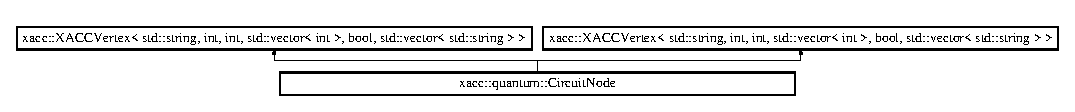
\includegraphics[height=1.060606cm]{a01292}
\end{center}
\end{figure}
\subsection*{Additional Inherited Members}


\subsection{Detailed Description}
\hyperlink{a01292}{Circuit\+Node} subclasses Q\+C\+I\+Vertex to provide the following parameters in the given order\+:

Parameters\+: Gate, Layer (ie time sequence), Gate Vertex Id, Qubit Ids that the gate acts on, enabled state, vector of parameters names 

The documentation for this class was generated from the following files\+:\begin{DoxyCompactItemize}
\item 
Gate\+Q\+I\+R.\+hpp\item 
Quantum\+Circuit.\+hpp\end{DoxyCompactItemize}

\hypertarget{a01908}{}\section{Simple\+Web\+:\+:Client$<$ socket\+\_\+type $>$ Class Template Reference}
\label{a01908}\index{Simple\+Web\+::\+Client$<$ socket\+\_\+type $>$@{Simple\+Web\+::\+Client$<$ socket\+\_\+type $>$}}
Inheritance diagram for Simple\+Web\+:\+:Client$<$ socket\+\_\+type $>$\+:\begin{figure}[H]
\begin{center}
\leavevmode
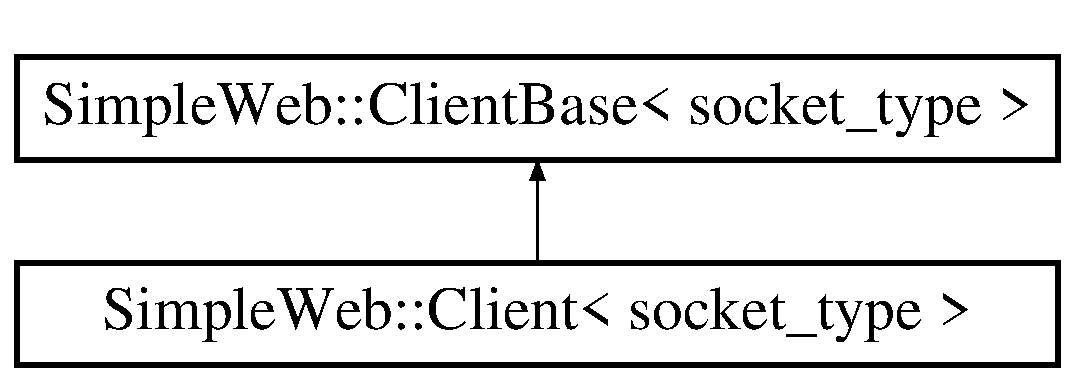
\includegraphics[height=2.000000cm]{a01908}
\end{center}
\end{figure}
\subsection*{Additional Inherited Members}


The documentation for this class was generated from the following file\+:\begin{DoxyCompactItemize}
\item 
client\+\_\+http.\+hpp\end{DoxyCompactItemize}

\hypertarget{a01924}{}\section{Simple\+Web\+:\+:Client$<$ H\+T\+TP $>$ Class Template Reference}
\label{a01924}\index{Simple\+Web\+::\+Client$<$ H\+T\+T\+P $>$@{Simple\+Web\+::\+Client$<$ H\+T\+T\+P $>$}}
Inheritance diagram for Simple\+Web\+:\+:Client$<$ H\+T\+TP $>$\+:\begin{figure}[H]
\begin{center}
\leavevmode
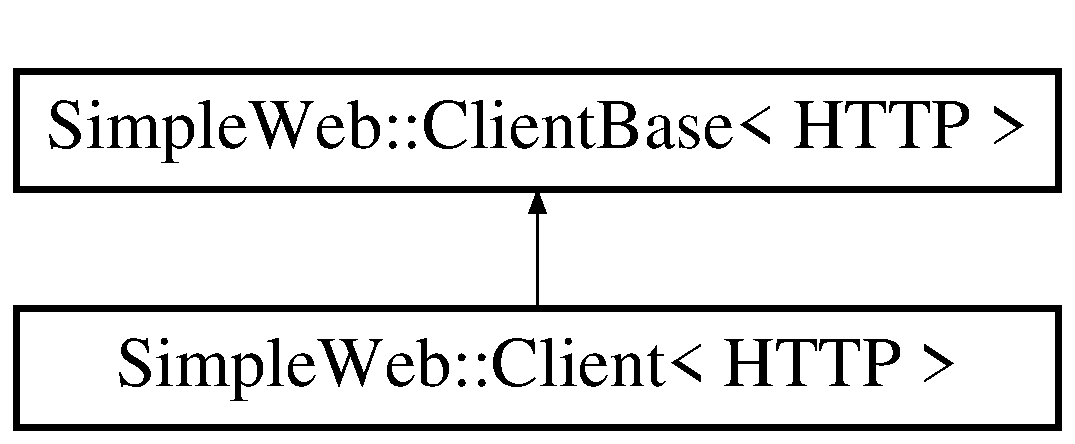
\includegraphics[height=2.000000cm]{a01924}
\end{center}
\end{figure}
\subsection*{Public Member Functions}
\begin{DoxyCompactItemize}
\item 
\mbox{\Hypertarget{a01924_a47655afc849e459096743876391dae17}\label{a01924_a47655afc849e459096743876391dae17}} 
{\bfseries Client} (const std\+::string \&server\+\_\+port\+\_\+path)
\end{DoxyCompactItemize}
\subsection*{Protected Member Functions}
\begin{DoxyCompactItemize}
\item 
\mbox{\Hypertarget{a01924_aebed110274c94b539e2d0a857c24991d}\label{a01924_aebed110274c94b539e2d0a857c24991d}} 
void {\bfseries connect} ()
\end{DoxyCompactItemize}
\subsection*{Additional Inherited Members}


The documentation for this class was generated from the following file\+:\begin{DoxyCompactItemize}
\item 
client\+\_\+http.\+hpp\end{DoxyCompactItemize}

\hypertarget{a01928}{}\section{Simple\+Web\+:\+:Client$<$ H\+T\+T\+PS $>$ Class Template Reference}
\label{a01928}\index{Simple\+Web\+::\+Client$<$ H\+T\+T\+P\+S $>$@{Simple\+Web\+::\+Client$<$ H\+T\+T\+P\+S $>$}}
Inheritance diagram for Simple\+Web\+:\+:Client$<$ H\+T\+T\+PS $>$\+:\begin{figure}[H]
\begin{center}
\leavevmode
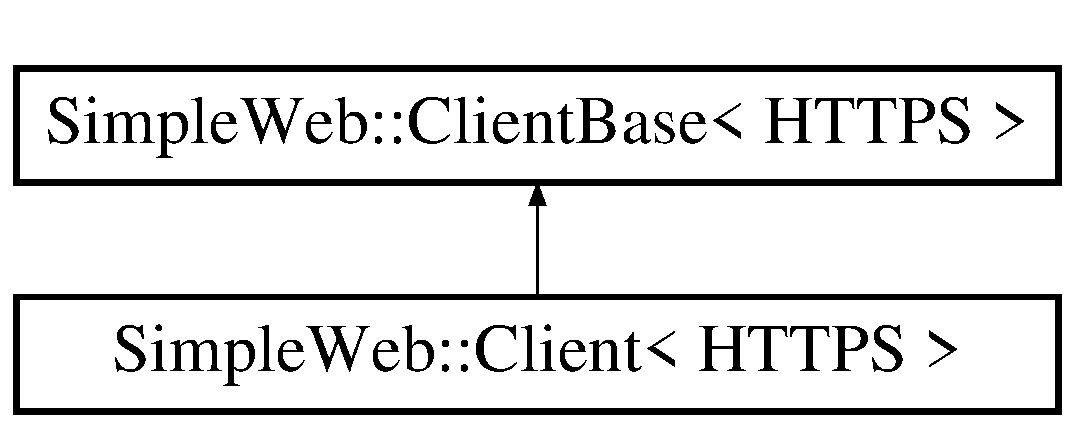
\includegraphics[height=2.000000cm]{a01928}
\end{center}
\end{figure}
\subsection*{Public Member Functions}
\begin{DoxyCompactItemize}
\item 
\mbox{\Hypertarget{a01928_abd87d3dc08c9fed3a60f18c749b8bacd}\label{a01928_abd87d3dc08c9fed3a60f18c749b8bacd}} 
{\bfseries Client} (const std\+::string \&server\+\_\+port\+\_\+path, bool verify\+\_\+certificate=true, const std\+::string \&cert\+\_\+file=std\+::string(), const std\+::string \&private\+\_\+key\+\_\+file=std\+::string(), const std\+::string \&verify\+\_\+file=std\+::string())
\end{DoxyCompactItemize}
\subsection*{Protected Member Functions}
\begin{DoxyCompactItemize}
\item 
\mbox{\Hypertarget{a01928_a833f6fd136e3158b873bee024d6e188c}\label{a01928_a833f6fd136e3158b873bee024d6e188c}} 
void {\bfseries connect} ()
\end{DoxyCompactItemize}
\subsection*{Protected Attributes}
\begin{DoxyCompactItemize}
\item 
\mbox{\Hypertarget{a01928_afe57679cc6153d5d1fe8abc94a8fa58a}\label{a01928_afe57679cc6153d5d1fe8abc94a8fa58a}} 
boost\+::asio\+::ssl\+::context {\bfseries context}
\end{DoxyCompactItemize}
\subsection*{Additional Inherited Members}


The documentation for this class was generated from the following file\+:\begin{DoxyCompactItemize}
\item 
client\+\_\+https.\+hpp\end{DoxyCompactItemize}

\hypertarget{a01912}{}\section{Simple\+Web\+:\+:Client\+Base$<$ socket\+\_\+type $>$ Class Template Reference}
\label{a01912}\index{Simple\+Web\+::\+Client\+Base$<$ socket\+\_\+type $>$@{Simple\+Web\+::\+Client\+Base$<$ socket\+\_\+type $>$}}
Inheritance diagram for Simple\+Web\+:\+:Client\+Base$<$ socket\+\_\+type $>$\+:\begin{figure}[H]
\begin{center}
\leavevmode
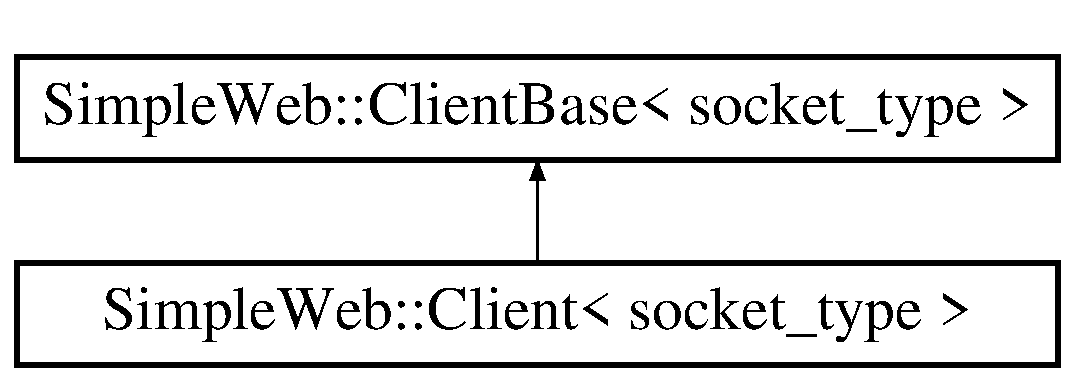
\includegraphics[height=2.000000cm]{a01912}
\end{center}
\end{figure}
\subsection*{Classes}
\begin{DoxyCompactItemize}
\item 
class \hyperlink{a01920}{Config}
\item 
class \hyperlink{a01916}{Response}
\end{DoxyCompactItemize}
\subsection*{Public Member Functions}
\begin{DoxyCompactItemize}
\item 
\mbox{\Hypertarget{a01912_ac8a838ace77f0a1a19b8cb03bdba7e74}\label{a01912_ac8a838ace77f0a1a19b8cb03bdba7e74}} 
std\+::shared\+\_\+ptr$<$ \hyperlink{a01916}{Response} $>$ {\bfseries request} (const std\+::string \&request\+\_\+type, const std\+::string \&path=\char`\"{}/\char`\"{}, boost\+::string\+\_\+ref content=\char`\"{}\char`\"{}, const std\+::map$<$ std\+::string, std\+::string $>$ \&header=std\+::map$<$ std\+::string, std\+::string $>$())
\item 
\mbox{\Hypertarget{a01912_aca6cb17dbea9adf0cf1daf9d1ea70f76}\label{a01912_aca6cb17dbea9adf0cf1daf9d1ea70f76}} 
std\+::shared\+\_\+ptr$<$ \hyperlink{a01916}{Response} $>$ {\bfseries request} (const std\+::string \&request\+\_\+type, const std\+::string \&path, std\+::iostream \&content, const std\+::map$<$ std\+::string, std\+::string $>$ \&header=std\+::map$<$ std\+::string, std\+::string $>$())
\item 
\mbox{\Hypertarget{a01912_ad21735a9bda2fae6aedd811efae981e1}\label{a01912_ad21735a9bda2fae6aedd811efae981e1}} 
void {\bfseries close} ()
\end{DoxyCompactItemize}
\subsection*{Public Attributes}
\begin{DoxyCompactItemize}
\item 
\mbox{\Hypertarget{a01912_af17ddd25319c4f9029969441dfd54eff}\label{a01912_af17ddd25319c4f9029969441dfd54eff}} 
\hyperlink{a01920}{Config} \hyperlink{a01912_af17ddd25319c4f9029969441dfd54eff}{config}
\begin{DoxyCompactList}\small\item\em Set before calling request. \end{DoxyCompactList}\end{DoxyCompactItemize}
\subsection*{Protected Member Functions}
\begin{DoxyCompactItemize}
\item 
\mbox{\Hypertarget{a01912_a4a74d44c9df44d0d469ad453bdac43bf}\label{a01912_a4a74d44c9df44d0d469ad453bdac43bf}} 
{\bfseries Client\+Base} (const std\+::string \&host\+\_\+port, unsigned short default\+\_\+port)
\item 
\mbox{\Hypertarget{a01912_ac511a8e5de870f533f8c28270c82dbfa}\label{a01912_ac511a8e5de870f533f8c28270c82dbfa}} 
std\+::pair$<$ std\+::string, unsigned short $>$ {\bfseries parse\+\_\+host\+\_\+port} (const std\+::string \&host\+\_\+port, unsigned short default\+\_\+port)
\item 
\mbox{\Hypertarget{a01912_a4c1f364a57eaef8fd10c29a82e475010}\label{a01912_a4c1f364a57eaef8fd10c29a82e475010}} 
virtual void {\bfseries connect} ()=0
\item 
\mbox{\Hypertarget{a01912_ab76f469e8f909bf046a80d5afad70469}\label{a01912_ab76f469e8f909bf046a80d5afad70469}} 
std\+::shared\+\_\+ptr$<$ boost\+::asio\+::deadline\+\_\+timer $>$ {\bfseries get\+\_\+timeout\+\_\+timer} (std\+::size\+\_\+t timeout=0)
\item 
\mbox{\Hypertarget{a01912_af11668a7cbf1a4e51f694c853cb70afe}\label{a01912_af11668a7cbf1a4e51f694c853cb70afe}} 
void {\bfseries parse\+\_\+response\+\_\+header} (const std\+::shared\+\_\+ptr$<$ \hyperlink{a01916}{Response} $>$ \&response) const
\item 
\mbox{\Hypertarget{a01912_afa5ddce26ed4c7570a764e2ff003fa25}\label{a01912_afa5ddce26ed4c7570a764e2ff003fa25}} 
std\+::shared\+\_\+ptr$<$ \hyperlink{a01916}{Response} $>$ {\bfseries request\+\_\+read} ()
\item 
\mbox{\Hypertarget{a01912_ae7fa171a9555114e702cafb3f85bc7d5}\label{a01912_ae7fa171a9555114e702cafb3f85bc7d5}} 
void {\bfseries request\+\_\+read\+\_\+chunked} (const std\+::shared\+\_\+ptr$<$ \hyperlink{a01916}{Response} $>$ \&response, boost\+::asio\+::streambuf \&streambuf)
\end{DoxyCompactItemize}
\subsection*{Protected Attributes}
\begin{DoxyCompactItemize}
\item 
\mbox{\Hypertarget{a01912_abe07c05fed46efc9e6aa76736961ae20}\label{a01912_abe07c05fed46efc9e6aa76736961ae20}} 
boost\+::asio\+::io\+\_\+service {\bfseries io\+\_\+service}
\item 
\mbox{\Hypertarget{a01912_a2001dc43f4c3ef1f07a86eea8fbf8082}\label{a01912_a2001dc43f4c3ef1f07a86eea8fbf8082}} 
boost\+::asio\+::ip\+::tcp\+::resolver {\bfseries resolver}
\item 
\mbox{\Hypertarget{a01912_a48b0e61c61cfc3d5307a0101cc30a28e}\label{a01912_a48b0e61c61cfc3d5307a0101cc30a28e}} 
std\+::unique\+\_\+ptr$<$ socket\+\_\+type $>$ {\bfseries socket}
\item 
\mbox{\Hypertarget{a01912_a2c0d5c3d38f4a6a21b67918199b498da}\label{a01912_a2c0d5c3d38f4a6a21b67918199b498da}} 
std\+::mutex {\bfseries socket\+\_\+mutex}
\item 
\mbox{\Hypertarget{a01912_a4436f29ffdce0b29b210cbecd972ffef}\label{a01912_a4436f29ffdce0b29b210cbecd972ffef}} 
std\+::string {\bfseries host}
\item 
\mbox{\Hypertarget{a01912_aadd3336b64a1f8d559af656554ddd0e9}\label{a01912_aadd3336b64a1f8d559af656554ddd0e9}} 
unsigned short {\bfseries port}
\end{DoxyCompactItemize}


The documentation for this class was generated from the following file\+:\begin{DoxyCompactItemize}
\item 
client\+\_\+http.\+hpp\end{DoxyCompactItemize}

\hypertarget{a02504}{}\section{xacc\+:\+:C\+L\+I\+Parser Class Reference}
\label{a02504}\index{xacc\+::\+C\+L\+I\+Parser@{xacc\+::\+C\+L\+I\+Parser}}


{\ttfamily \#include $<$C\+L\+I\+Parser.\+hpp$>$}

\subsection*{Public Member Functions}
\begin{DoxyCompactItemize}
\item 
\hyperlink{a02504_a3b170552b44c8a18dcd109cc6550df50}{C\+L\+I\+Parser} (int arc, char $\ast$$\ast$arv)
\item 
void \hyperlink{a02504_a9731a7f55a0ff2a0164e30f626797016}{parse} ()
\end{DoxyCompactItemize}
\subsection*{Protected Attributes}
\begin{DoxyCompactItemize}
\item 
int \hyperlink{a02504_afba175b92e7bc49e19660ef541db8cd5}{argc}
\item 
char $\ast$$\ast$ \hyperlink{a02504_aa269b5c9a78f2fe3e4ac48012eb3cc06}{argv}
\end{DoxyCompactItemize}


\subsection{Detailed Description}
The role of the \hyperlink{a02504}{C\+L\+I\+Parser} is to parse all command line options provided to an X\+A\+C\+C-\/enabled program. It takes upon construction to available argc and argv variables from the command line, and parses them to fill the \hyperlink{a02544}{Runtime\+Options} singleton and load any X\+A\+CC \hyperlink{a02448}{Compiler} or \hyperlink{a02432}{Accelerator} plugins.

It also queries all available Option\+Providers to display all available options to the X\+A\+CC user. 

\subsection{Constructor \& Destructor Documentation}
\mbox{\Hypertarget{a02504_a3b170552b44c8a18dcd109cc6550df50}\label{a02504_a3b170552b44c8a18dcd109cc6550df50}} 
\index{xacc\+::\+C\+L\+I\+Parser@{xacc\+::\+C\+L\+I\+Parser}!C\+L\+I\+Parser@{C\+L\+I\+Parser}}
\index{C\+L\+I\+Parser@{C\+L\+I\+Parser}!xacc\+::\+C\+L\+I\+Parser@{xacc\+::\+C\+L\+I\+Parser}}
\subsubsection{\texorpdfstring{C\+L\+I\+Parser()}{CLIParser()}}
{\footnotesize\ttfamily xacc\+::\+C\+L\+I\+Parser\+::\+C\+L\+I\+Parser (\begin{DoxyParamCaption}\item[{int}]{arc,  }\item[{char $\ast$$\ast$}]{arv }\end{DoxyParamCaption})\hspace{0.3cm}{\ttfamily [inline]}}

The constructor 

\subsection{Member Function Documentation}
\mbox{\Hypertarget{a02504_a9731a7f55a0ff2a0164e30f626797016}\label{a02504_a9731a7f55a0ff2a0164e30f626797016}} 
\index{xacc\+::\+C\+L\+I\+Parser@{xacc\+::\+C\+L\+I\+Parser}!parse@{parse}}
\index{parse@{parse}!xacc\+::\+C\+L\+I\+Parser@{xacc\+::\+C\+L\+I\+Parser}}
\subsubsection{\texorpdfstring{parse()}{parse()}}
{\footnotesize\ttfamily void xacc\+::\+C\+L\+I\+Parser\+::parse (\begin{DoxyParamCaption}{ }\end{DoxyParamCaption})\hspace{0.3cm}{\ttfamily [inline]}}

Parse the command line options. Provide a Boost options\+\_\+description built up and provided by all available Options\+Providers. This method also loads all Compilers and Accelerators available in the X\+A\+C\+C\+\_\+\+I\+N\+S\+T\+A\+L\+L\+\_\+\+D\+IR. 

\subsection{Member Data Documentation}
\mbox{\Hypertarget{a02504_afba175b92e7bc49e19660ef541db8cd5}\label{a02504_afba175b92e7bc49e19660ef541db8cd5}} 
\index{xacc\+::\+C\+L\+I\+Parser@{xacc\+::\+C\+L\+I\+Parser}!argc@{argc}}
\index{argc@{argc}!xacc\+::\+C\+L\+I\+Parser@{xacc\+::\+C\+L\+I\+Parser}}
\subsubsection{\texorpdfstring{argc}{argc}}
{\footnotesize\ttfamily int xacc\+::\+C\+L\+I\+Parser\+::argc\hspace{0.3cm}{\ttfamily [protected]}}

Argc, number of arguments \mbox{\Hypertarget{a02504_aa269b5c9a78f2fe3e4ac48012eb3cc06}\label{a02504_aa269b5c9a78f2fe3e4ac48012eb3cc06}} 
\index{xacc\+::\+C\+L\+I\+Parser@{xacc\+::\+C\+L\+I\+Parser}!argv@{argv}}
\index{argv@{argv}!xacc\+::\+C\+L\+I\+Parser@{xacc\+::\+C\+L\+I\+Parser}}
\subsubsection{\texorpdfstring{argv}{argv}}
{\footnotesize\ttfamily char$\ast$$\ast$ xacc\+::\+C\+L\+I\+Parser\+::argv\hspace{0.3cm}{\ttfamily [protected]}}

Argv, the command line arguments 

The documentation for this class was generated from the following file\+:\begin{DoxyCompactItemize}
\item 
C\+L\+I\+Parser.\+hpp\end{DoxyCompactItemize}

\hypertarget{a01300}{}\section{xacc\+:\+:quantum\+:\+:C\+N\+OT Class Reference}
\label{a01300}\index{xacc\+::quantum\+::\+C\+N\+OT@{xacc\+::quantum\+::\+C\+N\+OT}}
Inheritance diagram for xacc\+:\+:quantum\+:\+:C\+N\+OT\+:\begin{figure}[H]
\begin{center}
\leavevmode
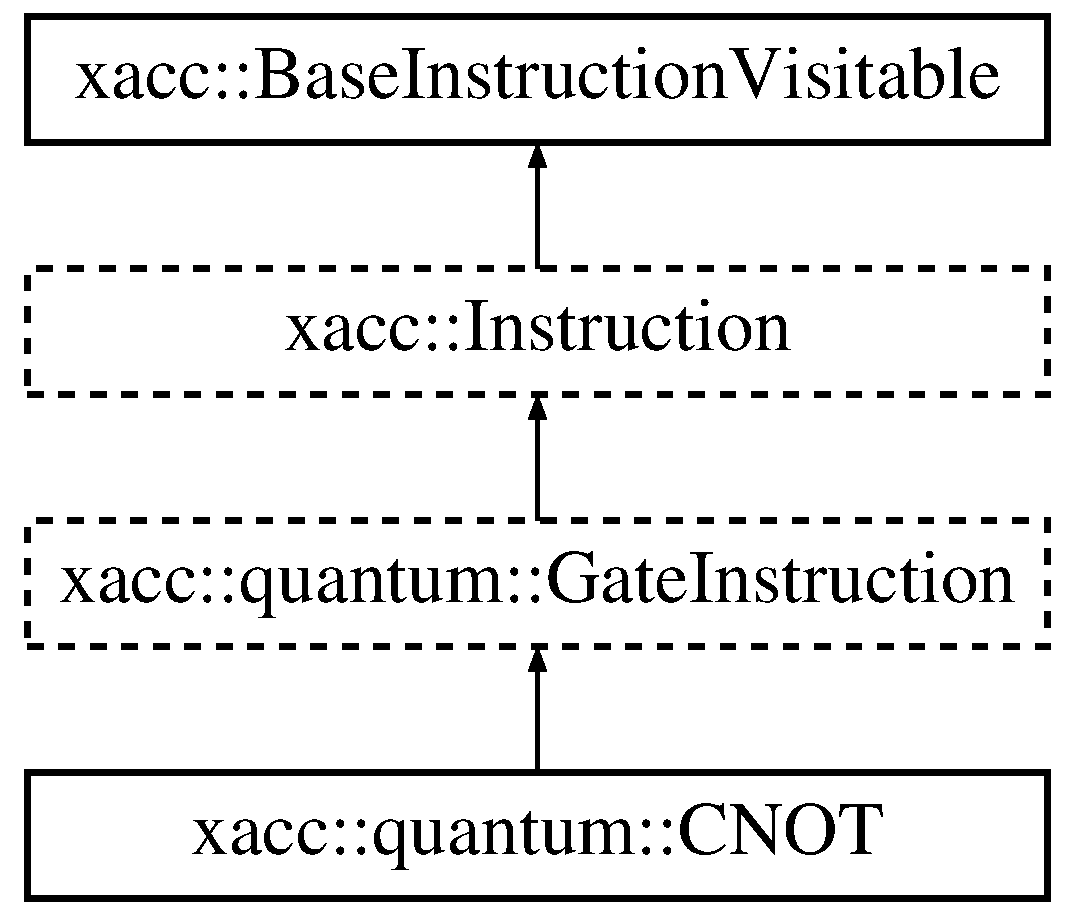
\includegraphics[height=4.000000cm]{a01300}
\end{center}
\end{figure}
\subsection*{Public Member Functions}
\begin{DoxyCompactItemize}
\item 
\mbox{\Hypertarget{a01300_ad3d460779a27affa317dd4f3a88268b3}\label{a01300_ad3d460779a27affa317dd4f3a88268b3}} 
{\bfseries C\+N\+OT} (std\+::vector$<$ int $>$ \hyperlink{a01276_a2a56be6c2519ea65df4d06f4abae1393}{qbits})
\item 
\mbox{\Hypertarget{a01300_a15efcb44477dde4b6151fe1776a73ddc}\label{a01300_a15efcb44477dde4b6151fe1776a73ddc}} 
{\bfseries C\+N\+OT} (int srcqbit, int tgtqbit)
\end{DoxyCompactItemize}
\subsection*{Additional Inherited Members}


The documentation for this class was generated from the following files\+:\begin{DoxyCompactItemize}
\item 
C\+N\+O\+T.\+hpp\item 
C\+N\+O\+T.\+cpp\end{DoxyCompactItemize}

\hypertarget{a02448}{}\section{xacc\+:\+:Compiler Class Reference}
\label{a02448}\index{xacc\+::\+Compiler@{xacc\+::\+Compiler}}


{\ttfamily \#include $<$Compiler.\+hpp$>$}

Inheritance diagram for xacc\+:\+:Compiler\+:\begin{figure}[H]
\begin{center}
\leavevmode
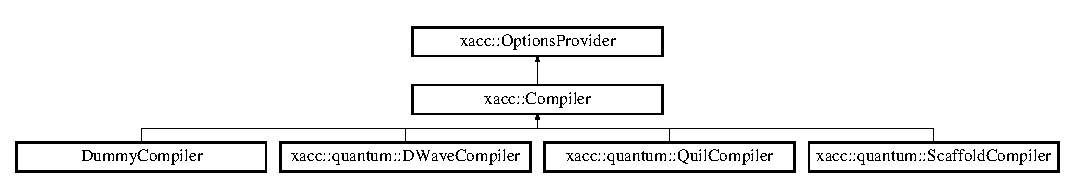
\includegraphics[height=2.079208cm]{a02448}
\end{center}
\end{figure}
\subsection*{Public Member Functions}
\begin{DoxyCompactItemize}
\item 
virtual std\+::shared\+\_\+ptr$<$ \hyperlink{a02480}{IR} $>$ \hyperlink{a02448_a546a40c95bb93af6a0c0ac48dbeaffc8}{compile} (const std\+::string \&src, std\+::shared\+\_\+ptr$<$ \hyperlink{a02432}{Accelerator} $>$ acc)=0
\item 
virtual std\+::shared\+\_\+ptr$<$ \hyperlink{a02480}{IR} $>$ \hyperlink{a02448_a9092f5f779b570c91569b59621280c04}{compile} (const std\+::string \&src)=0
\item 
virtual const std\+::string \hyperlink{a02448_a87fca9100e6462122f5b687c3a0fb3fb}{get\+Name} ()=0
\item 
virtual std\+::shared\+\_\+ptr$<$ options\+\_\+description $>$ \hyperlink{a02448_a9f5a8965c9c2dd895016d18264ebbe92}{get\+Options} ()
\item 
virtual \hyperlink{a02448_a5d0b012687d9b44893872eaa81e47b38}{$\sim$\+Compiler} ()
\end{DoxyCompactItemize}
\subsection*{Protected Attributes}
\begin{DoxyCompactItemize}
\item 
std\+::string \hyperlink{a02448_a0ad81c816c09e5113d03cdc02165c453}{kernel\+Source}
\item 
std\+::shared\+\_\+ptr$<$ \hyperlink{a02432}{Accelerator} $>$ \hyperlink{a02448_ad4cbb467fa7e377bac6c054ffcb22b7c}{accelerator}
\end{DoxyCompactItemize}


\subsection{Detailed Description}
The \hyperlink{a02448}{Compiler} class provides an extensible interface for injecting custom compilation mechanisms into the X\+A\+CC framework. Implementations provide a compile method that takes the kernel source code string, performs compiler-\/specific compilation mechanism, and returns a valid X\+A\+CC \hyperlink{a02480}{IR} instance modeling the result of the compilation. 

\subsection{Constructor \& Destructor Documentation}
\mbox{\Hypertarget{a02448_a5d0b012687d9b44893872eaa81e47b38}\label{a02448_a5d0b012687d9b44893872eaa81e47b38}} 
\index{xacc\+::\+Compiler@{xacc\+::\+Compiler}!````~Compiler@{$\sim$\+Compiler}}
\index{````~Compiler@{$\sim$\+Compiler}!xacc\+::\+Compiler@{xacc\+::\+Compiler}}
\subsubsection{\texorpdfstring{$\sim$\+Compiler()}{~Compiler()}}
{\footnotesize\ttfamily virtual xacc\+::\+Compiler\+::$\sim$\+Compiler (\begin{DoxyParamCaption}{ }\end{DoxyParamCaption})\hspace{0.3cm}{\ttfamily [inline]}, {\ttfamily [virtual]}}

The destructor 

\subsection{Member Function Documentation}
\mbox{\Hypertarget{a02448_a546a40c95bb93af6a0c0ac48dbeaffc8}\label{a02448_a546a40c95bb93af6a0c0ac48dbeaffc8}} 
\index{xacc\+::\+Compiler@{xacc\+::\+Compiler}!compile@{compile}}
\index{compile@{compile}!xacc\+::\+Compiler@{xacc\+::\+Compiler}}
\subsubsection{\texorpdfstring{compile()}{compile()}\hspace{0.1cm}{\footnotesize\ttfamily [1/2]}}
{\footnotesize\ttfamily virtual std\+::shared\+\_\+ptr$<$\hyperlink{a02480}{IR}$>$ xacc\+::\+Compiler\+::compile (\begin{DoxyParamCaption}\item[{const std\+::string \&}]{src,  }\item[{std\+::shared\+\_\+ptr$<$ \hyperlink{a02432}{Accelerator} $>$}]{acc }\end{DoxyParamCaption})\hspace{0.3cm}{\ttfamily [pure virtual]}}

This method is to be implemented by derived Compilers and is in charge of executing the compilation mechanism on the provided source string. Implementations also are given access to the \hyperlink{a02432}{Accelerator} that this source code is intended for.


\begin{DoxyParams}{Parameters}
{\em src} & The kernel source string. \\
\hline
{\em acc} & The \hyperlink{a02432}{Accelerator} this code will be executed on \\
\hline
\end{DoxyParams}
\begin{DoxyReturn}{Returns}
ir Intermediate representation for provided source kernel code. 
\end{DoxyReturn}


Implemented in \hyperlink{a02500_acc75af818d62ba22d1dd7de3b66c4baf}{Dummy\+Compiler}, \hyperlink{a01236_a7caede75bb2304ba405966651b115543}{xacc\+::quantum\+::\+Scaffold\+Compiler}, \hyperlink{a01204_a2421482415ca4e09963ea4ecddff8100}{xacc\+::quantum\+::\+Quil\+Compiler}, and \hyperlink{a01252_a0f7f6b10b4a881cb27b36eaa6d39e7b1}{xacc\+::quantum\+::\+D\+Wave\+Compiler}.

\mbox{\Hypertarget{a02448_a9092f5f779b570c91569b59621280c04}\label{a02448_a9092f5f779b570c91569b59621280c04}} 
\index{xacc\+::\+Compiler@{xacc\+::\+Compiler}!compile@{compile}}
\index{compile@{compile}!xacc\+::\+Compiler@{xacc\+::\+Compiler}}
\subsubsection{\texorpdfstring{compile()}{compile()}\hspace{0.1cm}{\footnotesize\ttfamily [2/2]}}
{\footnotesize\ttfamily virtual std\+::shared\+\_\+ptr$<$\hyperlink{a02480}{IR}$>$ xacc\+::\+Compiler\+::compile (\begin{DoxyParamCaption}\item[{const std\+::string \&}]{src }\end{DoxyParamCaption})\hspace{0.3cm}{\ttfamily [pure virtual]}}

This method is to be implemented by derived Compilers and is in charge of executing the compilation mechanism on the provided source string. 
\begin{DoxyParams}{Parameters}
{\em src} & \\
\hline
\end{DoxyParams}
\begin{DoxyReturn}{Returns}

\end{DoxyReturn}


Implemented in \hyperlink{a02500_a40d7cc3bbc72a2ce9362136b3b83245c}{Dummy\+Compiler}, \hyperlink{a01236_a3736ecc229fe6acdd4c991e85d7a1f08}{xacc\+::quantum\+::\+Scaffold\+Compiler}, \hyperlink{a01204_adf4d321ecb0df3fa7728999f941c83b2}{xacc\+::quantum\+::\+Quil\+Compiler}, and \hyperlink{a01252_a893e1d1c81a8aaf6e2435c9bceab575e}{xacc\+::quantum\+::\+D\+Wave\+Compiler}.

\mbox{\Hypertarget{a02448_a87fca9100e6462122f5b687c3a0fb3fb}\label{a02448_a87fca9100e6462122f5b687c3a0fb3fb}} 
\index{xacc\+::\+Compiler@{xacc\+::\+Compiler}!get\+Name@{get\+Name}}
\index{get\+Name@{get\+Name}!xacc\+::\+Compiler@{xacc\+::\+Compiler}}
\subsubsection{\texorpdfstring{get\+Name()}{getName()}}
{\footnotesize\ttfamily virtual const std\+::string xacc\+::\+Compiler\+::get\+Name (\begin{DoxyParamCaption}{ }\end{DoxyParamCaption})\hspace{0.3cm}{\ttfamily [pure virtual]}}

Return the name of this \hyperlink{a02448}{Compiler} \begin{DoxyReturn}{Returns}
name \hyperlink{a02448}{Compiler} name 
\end{DoxyReturn}


Implemented in \hyperlink{a02500_a76460cb78671dc2cf42f2bebf8fb80c7}{Dummy\+Compiler}, \hyperlink{a01236_a3f537054a3924a1d14f4ceb0f0181161}{xacc\+::quantum\+::\+Scaffold\+Compiler}, \hyperlink{a01204_ae7d52140b6dd52730edc6e38ae48f437}{xacc\+::quantum\+::\+Quil\+Compiler}, and \hyperlink{a01252_a8a180031ae563e1a9aac611e8066c181}{xacc\+::quantum\+::\+D\+Wave\+Compiler}.

\mbox{\Hypertarget{a02448_a9f5a8965c9c2dd895016d18264ebbe92}\label{a02448_a9f5a8965c9c2dd895016d18264ebbe92}} 
\index{xacc\+::\+Compiler@{xacc\+::\+Compiler}!get\+Options@{get\+Options}}
\index{get\+Options@{get\+Options}!xacc\+::\+Compiler@{xacc\+::\+Compiler}}
\subsubsection{\texorpdfstring{get\+Options()}{getOptions()}}
{\footnotesize\ttfamily virtual std\+::shared\+\_\+ptr$<$options\+\_\+description$>$ xacc\+::\+Compiler\+::get\+Options (\begin{DoxyParamCaption}{ }\end{DoxyParamCaption})\hspace{0.3cm}{\ttfamily [inline]}, {\ttfamily [virtual]}}

Return an empty options\+\_\+description, this is for subclasses to implement. 

Implements \hyperlink{a02536_a6d150954f852109bfe2c1ae90222926f}{xacc\+::\+Options\+Provider}.



\subsection{Member Data Documentation}
\mbox{\Hypertarget{a02448_ad4cbb467fa7e377bac6c054ffcb22b7c}\label{a02448_ad4cbb467fa7e377bac6c054ffcb22b7c}} 
\index{xacc\+::\+Compiler@{xacc\+::\+Compiler}!accelerator@{accelerator}}
\index{accelerator@{accelerator}!xacc\+::\+Compiler@{xacc\+::\+Compiler}}
\subsubsection{\texorpdfstring{accelerator}{accelerator}}
{\footnotesize\ttfamily std\+::shared\+\_\+ptr$<$\hyperlink{a02432}{Accelerator}$>$ xacc\+::\+Compiler\+::accelerator\hspace{0.3cm}{\ttfamily [protected]}}

Reference to the \hyperlink{a02432}{Accelerator} that this compiler is targeting. \mbox{\Hypertarget{a02448_a0ad81c816c09e5113d03cdc02165c453}\label{a02448_a0ad81c816c09e5113d03cdc02165c453}} 
\index{xacc\+::\+Compiler@{xacc\+::\+Compiler}!kernel\+Source@{kernel\+Source}}
\index{kernel\+Source@{kernel\+Source}!xacc\+::\+Compiler@{xacc\+::\+Compiler}}
\subsubsection{\texorpdfstring{kernel\+Source}{kernelSource}}
{\footnotesize\ttfamily std\+::string xacc\+::\+Compiler\+::kernel\+Source\hspace{0.3cm}{\ttfamily [protected]}}

Reference to the provided kernel source code string 

The documentation for this class was generated from the following file\+:\begin{DoxyCompactItemize}
\item 
Compiler.\+hpp\end{DoxyCompactItemize}

\hypertarget{a01304}{}\section{xacc\+:\+:quantum\+:\+:Conditional\+Function Class Reference}
\label{a01304}\index{xacc\+::quantum\+::\+Conditional\+Function@{xacc\+::quantum\+::\+Conditional\+Function}}
Inheritance diagram for xacc\+:\+:quantum\+:\+:Conditional\+Function\+:\begin{figure}[H]
\begin{center}
\leavevmode
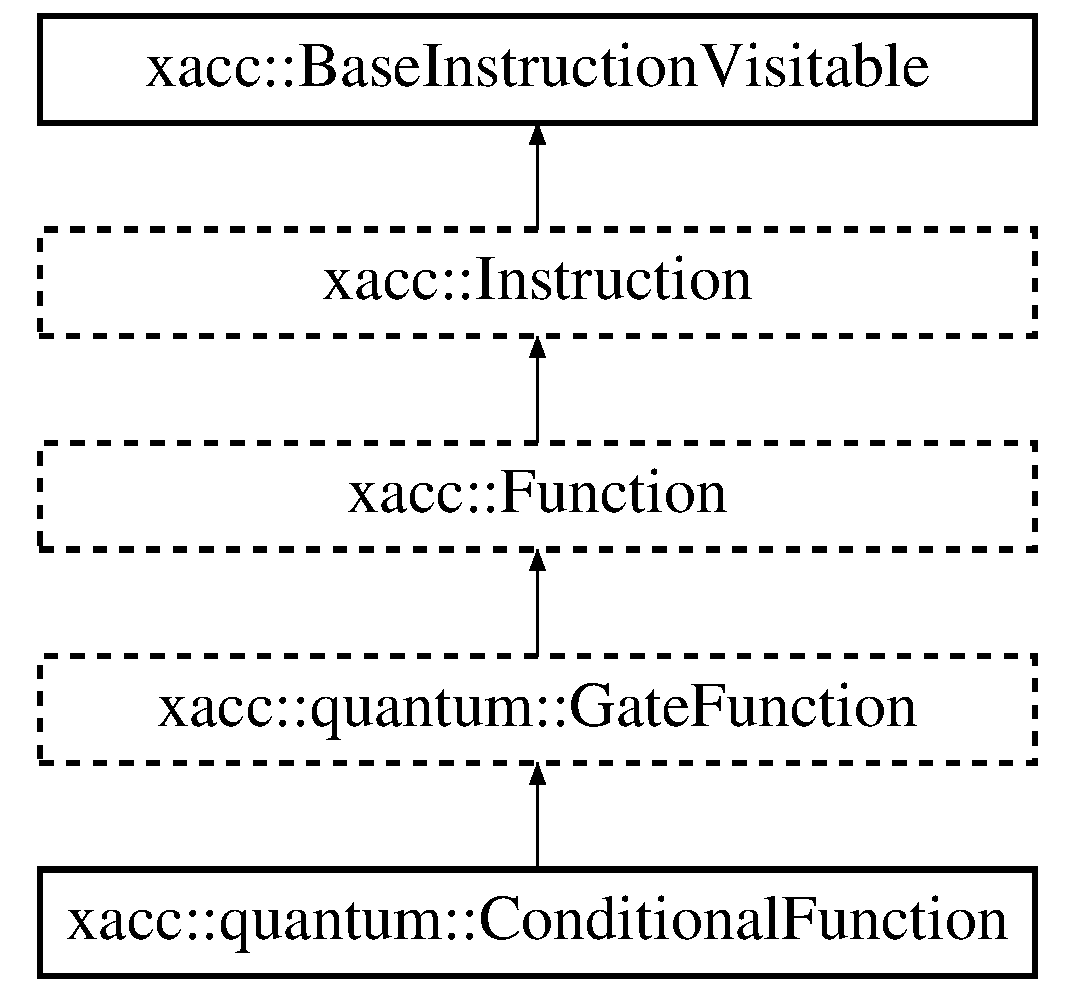
\includegraphics[height=5.000000cm]{a01304}
\end{center}
\end{figure}
\subsection*{Public Member Functions}
\begin{DoxyCompactItemize}
\item 
\mbox{\Hypertarget{a01304_aa28610a08ae04d62ccdd8359433100c3}\label{a01304_aa28610a08ae04d62ccdd8359433100c3}} 
{\bfseries Conditional\+Function} (int qbit)
\item 
virtual void \hyperlink{a01304_a6aedad20f96390880efdc0a476b3273f}{add\+Instruction} (Inst\+Ptr instruction)
\item 
\mbox{\Hypertarget{a01304_a804317333b6677a041a3071b5108c0df}\label{a01304_a804317333b6677a041a3071b5108c0df}} 
const int {\bfseries get\+Conditional\+Qubit} ()
\item 
\mbox{\Hypertarget{a01304_a709c236a5beb62d9a3bd5265196fb6c9}\label{a01304_a709c236a5beb62d9a3bd5265196fb6c9}} 
void {\bfseries evaluate} (const int acc\+Bit\+State)
\item 
virtual const std\+::string \hyperlink{a01304_aca7a5f849fece6fc28a904efee9a3370}{to\+String} (const std\+::string \&buffer\+Var\+Name)
\end{DoxyCompactItemize}
\subsection*{Protected Attributes}
\begin{DoxyCompactItemize}
\item 
\mbox{\Hypertarget{a01304_a0310536801417c0eded28a4dea1efa44}\label{a01304_a0310536801417c0eded28a4dea1efa44}} 
int {\bfseries qbit\+Idx}
\end{DoxyCompactItemize}
\subsection*{Additional Inherited Members}


\subsection{Member Function Documentation}
\mbox{\Hypertarget{a01304_a6aedad20f96390880efdc0a476b3273f}\label{a01304_a6aedad20f96390880efdc0a476b3273f}} 
\index{xacc\+::quantum\+::\+Conditional\+Function@{xacc\+::quantum\+::\+Conditional\+Function}!add\+Instruction@{add\+Instruction}}
\index{add\+Instruction@{add\+Instruction}!xacc\+::quantum\+::\+Conditional\+Function@{xacc\+::quantum\+::\+Conditional\+Function}}
\subsubsection{\texorpdfstring{add\+Instruction()}{addInstruction()}}
{\footnotesize\ttfamily void xacc\+::quantum\+::\+Conditional\+Function\+::add\+Instruction (\begin{DoxyParamCaption}\item[{Inst\+Ptr}]{instruction }\end{DoxyParamCaption})\hspace{0.3cm}{\ttfamily [virtual]}}

Add an instruction to this quantum intermediate representation.


\begin{DoxyParams}{Parameters}
{\em instruction} & \\
\hline
\end{DoxyParams}


Reimplemented from \hyperlink{a01272_a892fb69a10f0a7cb5abdab4cca61b80a}{xacc\+::quantum\+::\+Gate\+Function}.

\mbox{\Hypertarget{a01304_aca7a5f849fece6fc28a904efee9a3370}\label{a01304_aca7a5f849fece6fc28a904efee9a3370}} 
\index{xacc\+::quantum\+::\+Conditional\+Function@{xacc\+::quantum\+::\+Conditional\+Function}!to\+String@{to\+String}}
\index{to\+String@{to\+String}!xacc\+::quantum\+::\+Conditional\+Function@{xacc\+::quantum\+::\+Conditional\+Function}}
\subsubsection{\texorpdfstring{to\+String()}{toString()}}
{\footnotesize\ttfamily const std\+::string xacc\+::quantum\+::\+Conditional\+Function\+::to\+String (\begin{DoxyParamCaption}\item[{const std\+::string \&}]{buffer\+Var\+Name }\end{DoxyParamCaption})\hspace{0.3cm}{\ttfamily [virtual]}}

Return an assembly-\/like string representation for this function . 
\begin{DoxyParams}{Parameters}
{\em buffer\+Var\+Name} & \\
\hline
\end{DoxyParams}
\begin{DoxyReturn}{Returns}

\end{DoxyReturn}


Reimplemented from \hyperlink{a01272_aa1950776ae84bad2d0795a0441f910e7}{xacc\+::quantum\+::\+Gate\+Function}.



The documentation for this class was generated from the following files\+:\begin{DoxyCompactItemize}
\item 
Conditional\+Function.\+hpp\item 
Conditional\+Function.\+cpp\end{DoxyCompactItemize}



 layout\+: post title\+: About the Gravity Theme permalink\+: /about/about-\/gravity-\/theme \subsection*{category\+: about }

\subsection*{Gravity}

Minimal, text based, liberal Jekyll theme~\newline
for sharing your awesome ideas.

~\newline
 \begin{center}\end{center} 

\begin{center}{\bfseries Get up and running with Gravity}\end{center} 

\begin{center}\end{center}  ~\newline
   {\bfseries Posting}  

  \begin{DoxyVerb}  - Create a .markdown file inside <code class="highlighter-rouge">_posts</code> folder.<br>
  - Name the file according to the format YY-MM-DD-[short name for your post].<br>  <code>2016-03-30-i-love-design.markdown</code><br>
  - Write the <a href="jekyll">Front Matter</a> and content in the file.<br>
  <div class="example">
    <span class='manual'>FORMAT</span><BR>
    <pre>---
\end{DoxyVerb}
 layout\+: post $\vert$ default $\vert$ page title\+: String Post Title date\+: Time Stamp categories\+: String $\vert$ Array of Strings Category / Categories  ---  

 
\begin{DoxyPre}---
layout: post
title:  "The One with the Blackout"
date:   2016-03-30 19:45:31 +0530
categories: ["life", "friends"]
---\end{DoxyPre}
 

  

~\newline
   {\bfseries Create Pages}  

  \begin{DoxyVerb}  - Create a .md file in the root directory.<br>
  - Name the file with the desired page link name.<br>  <code>about.md</code><br><code>design.md</code><br>
  - Write the <a href="jekyll">Front Matter</a> and content in the file.
  <div class="example">
    <span class='manual'>FORMAT</span><BR>
    <pre>---
\end{DoxyVerb}
 layout\+: page title\+: String Title of the webpage permalink\+: / String / Permalink for the webpage tagline\+: String Optional Gravity Feature \+: Tagline for the page ---  

 
\begin{DoxyPre}---
layout: page
title:  "Science"
permalink:   /science/
tagline : "Humanity is overrated."
---\end{DoxyPre}
 

  

~\newline
   {\bfseries Create Archives/ Category Pages}~\newline
 ~\newline
  

 Introducing {\bfseries Archive Pages}.~\newline


  You can display a list of all the post corresponding to a particular category on a standalone Page using the {\ttfamily \textquotesingle{}archive\textquotesingle{}} layout.   ~\newline




  \begin{DoxyVerb}  - Create a .md file in the root directory.<br>
  - Name the file. Preferred name will be the name of the category<br>  <code>life.md</code><br>
  - Write the <a href="jekyll">Front Matter</a> and content in the file.
  <div class="example">
    <span class='manual'>FORMAT</span><BR>
<pre>---
\end{DoxyVerb}
 layout\+: archive Archive Page Layout title\+: String Title of the webpage permalink\+: / String / Permalink for the webpage tagline\+: String  Tagline for the page category \+: String  Name of the category of which the page will show posts. ---  

 
\begin{DoxyPre}---
layout: archive
title:  "Design"
permalink : "Design"
category: "design"
tagline: "It's all about perception."
---\end{DoxyPre}
 ~\newline
  
\hypertarget{a01952}{}\section{Simple\+Web\+:\+:Server\+Base$<$ socket\+\_\+type $>$\+:\+:Config Class Reference}
\label{a01952}\index{Simple\+Web\+::\+Server\+Base$<$ socket\+\_\+type $>$\+::\+Config@{Simple\+Web\+::\+Server\+Base$<$ socket\+\_\+type $>$\+::\+Config}}
\subsection*{Public Attributes}
\begin{DoxyCompactItemize}
\item 
\mbox{\Hypertarget{a01952_aa80030952ff056db08f736d5537bd2c9}\label{a01952_aa80030952ff056db08f736d5537bd2c9}} 
unsigned short \hyperlink{a01952_aa80030952ff056db08f736d5537bd2c9}{port}
\begin{DoxyCompactList}\small\item\em Port number to use. Defaults to 80 for H\+T\+TP and 443 for H\+T\+T\+PS. \end{DoxyCompactList}\item 
\mbox{\Hypertarget{a01952_abfbbfc38bfd2887739676424509dbb45}\label{a01952_abfbbfc38bfd2887739676424509dbb45}} 
size\+\_\+t \hyperlink{a01952_abfbbfc38bfd2887739676424509dbb45}{thread\+\_\+pool\+\_\+size} =1
\begin{DoxyCompactList}\small\item\em Number of threads that the server will use when start() is called. Defaults to 1 thread. \end{DoxyCompactList}\item 
\mbox{\Hypertarget{a01952_aa27e09c83d7e26dff6e72e8d1084d5a0}\label{a01952_aa27e09c83d7e26dff6e72e8d1084d5a0}} 
size\+\_\+t \hyperlink{a01952_aa27e09c83d7e26dff6e72e8d1084d5a0}{timeout\+\_\+request} =5
\begin{DoxyCompactList}\small\item\em Timeout on request handling. Defaults to 5 seconds. \end{DoxyCompactList}\item 
\mbox{\Hypertarget{a01952_ac1f74ff91196c3a72446786b54a77b58}\label{a01952_ac1f74ff91196c3a72446786b54a77b58}} 
size\+\_\+t \hyperlink{a01952_ac1f74ff91196c3a72446786b54a77b58}{timeout\+\_\+content} =300
\begin{DoxyCompactList}\small\item\em Timeout on content handling. Defaults to 300 seconds. \end{DoxyCompactList}\item 
std\+::string \hyperlink{a01952_add7a705aca3533bf0371708b19bb691c}{address}
\item 
\mbox{\Hypertarget{a01952_aab9c347da5390b176d37dac2dfbd9fae}\label{a01952_aab9c347da5390b176d37dac2dfbd9fae}} 
bool \hyperlink{a01952_aab9c347da5390b176d37dac2dfbd9fae}{reuse\+\_\+address} =true
\begin{DoxyCompactList}\small\item\em Set to false to avoid binding the socket to an address that is already in use. Defaults to true. \end{DoxyCompactList}\end{DoxyCompactItemize}
\subsection*{Friends}
\begin{DoxyCompactItemize}
\item 
\mbox{\Hypertarget{a01952_a01d54a7e16ca437c98ec571deca98dfc}\label{a01952_a01d54a7e16ca437c98ec571deca98dfc}} 
class {\bfseries Server\+Base$<$ socket\+\_\+type $>$}
\end{DoxyCompactItemize}


\subsection{Member Data Documentation}
\mbox{\Hypertarget{a01952_add7a705aca3533bf0371708b19bb691c}\label{a01952_add7a705aca3533bf0371708b19bb691c}} 
\index{Simple\+Web\+::\+Server\+Base\+::\+Config@{Simple\+Web\+::\+Server\+Base\+::\+Config}!address@{address}}
\index{address@{address}!Simple\+Web\+::\+Server\+Base\+::\+Config@{Simple\+Web\+::\+Server\+Base\+::\+Config}}
\subsubsection{\texorpdfstring{address}{address}}
{\footnotesize\ttfamily template$<$class socket\+\_\+type$>$ \\
std\+::string \hyperlink{a01936}{Simple\+Web\+::\+Server\+Base}$<$ socket\+\_\+type $>$\+::Config\+::address}

I\+Pv4 address in dotted decimal form or I\+Pv6 address in hexadecimal notation. If empty, the address will be any address. 

The documentation for this class was generated from the following file\+:\begin{DoxyCompactItemize}
\item 
server\+\_\+http.\+hpp\end{DoxyCompactItemize}

\hypertarget{a01352}{}\section{boost\+:\+:dll\+:\+:detail\+:\+:constructor$<$ Signature $>$ Struct Template Reference}
\label{a01352}\index{boost\+::dll\+::detail\+::constructor$<$ Signature $>$@{boost\+::dll\+::detail\+::constructor$<$ Signature $>$}}


{\ttfamily \#include $<$ctor\+\_\+dtor.\+hpp$>$}



\subsection{Detailed Description}
\subsubsection*{template$<$typename Signature$>$\newline
struct boost\+::dll\+::detail\+::constructor$<$ Signature $>$}

This class stores a constructor.

In some compilers there are several constructors in code, which may include an allocating one. This can be used if the imported class shall be put on the heap, which is why the class provied both types. 

The documentation for this struct was generated from the following file\+:\begin{DoxyCompactItemize}
\item 
ctor\+\_\+dtor.\+hpp\end{DoxyCompactItemize}

\hypertarget{a01356}{}\section{boost\+:\+:dll\+:\+:detail\+:\+:constructor$<$ Class(Args...)$>$ Struct Template Reference}
\label{a01356}\index{boost\+::dll\+::detail\+::constructor$<$ Class(\+Args...)$>$@{boost\+::dll\+::detail\+::constructor$<$ Class(\+Args...)$>$}}
\subsection*{Public Types}
\begin{DoxyCompactItemize}
\item 
\mbox{\Hypertarget{a01356_ab765d8c7c083efce92a933c806a41e81}\label{a01356_ab765d8c7c083efce92a933c806a41e81}} 
typedef \hyperlink{a01412}{detail\+::get\+\_\+mem\+\_\+fn\+\_\+type}$<$ Class, void(Args...)$>$\+::mem\+\_\+fn {\bfseries standard\+\_\+t}
\item 
\mbox{\Hypertarget{a01356_a19159ea77e5c102bd216195b32045677}\label{a01356_a19159ea77e5c102bd216195b32045677}} 
typedef Class $\ast$($\ast$ {\bfseries allocating\+\_\+t}) (Args...)
\end{DoxyCompactItemize}
\subsection*{Public Member Functions}
\begin{DoxyCompactItemize}
\item 
\mbox{\Hypertarget{a01356_a2b0dbd4b6c5fb1c8fa284b64f85e3caa}\label{a01356_a2b0dbd4b6c5fb1c8fa284b64f85e3caa}} 
void \hyperlink{a01356_a2b0dbd4b6c5fb1c8fa284b64f85e3caa}{call\+\_\+standard} (Class $\ast$const ptr, Args...\+args)
\begin{DoxyCompactList}\small\item\em Call the standard contructor. \end{DoxyCompactList}\item 
\mbox{\Hypertarget{a01356_a9674344355e9759b8f60a4eb92e718af}\label{a01356_a9674344355e9759b8f60a4eb92e718af}} 
Class $\ast$ \hyperlink{a01356_a9674344355e9759b8f60a4eb92e718af}{call\+\_\+allocating} (Args...\+args)
\begin{DoxyCompactList}\small\item\em Call the deleting destructor. \end{DoxyCompactList}\item 
\mbox{\Hypertarget{a01356_a8f7a1ee62ed8cd923a05f12544d10787}\label{a01356_a8f7a1ee62ed8cd923a05f12544d10787}} 
bool \hyperlink{a01356_a8f7a1ee62ed8cd923a05f12544d10787}{has\+\_\+allocating} () const
\begin{DoxyCompactList}\small\item\em True if a allocating constructor could be loaded. \end{DoxyCompactList}\item 
\mbox{\Hypertarget{a01356_a30a1be17551af78128f3f0d10fd0b5e9}\label{a01356_a30a1be17551af78128f3f0d10fd0b5e9}} 
bool \hyperlink{a01356_a30a1be17551af78128f3f0d10fd0b5e9}{has\+\_\+standard} () const
\begin{DoxyCompactList}\small\item\em True if a standard constructor could be loaded. \end{DoxyCompactList}\item 
\mbox{\Hypertarget{a01356_a4fd80b98d5c5ea2d9482c8f30657ec40}\label{a01356_a4fd80b98d5c5ea2d9482c8f30657ec40}} 
bool \hyperlink{a01356_a4fd80b98d5c5ea2d9482c8f30657ec40}{is\+\_\+empty} () const
\begin{DoxyCompactList}\small\item\em False if neither the allocating nor the standard constructor is available. \end{DoxyCompactList}\item 
\mbox{\Hypertarget{a01356_a6ae77617757558a1b0177d6a2cae9827}\label{a01356_a6ae77617757558a1b0177d6a2cae9827}} 
{\bfseries constructor} (const \hyperlink{a01352}{constructor} \&)=default
\item 
\mbox{\Hypertarget{a01356_a403d27f9f509c0ce4e66d4713ca2affc}\label{a01356_a403d27f9f509c0ce4e66d4713ca2affc}} 
{\bfseries constructor} (standard\+\_\+t \hyperlink{a01356_a6cbccda8c81959e8e3bba7da28cada5d}{standard}, allocating\+\_\+t \hyperlink{a01356_a13c90a276dc453ca83da117ffc552362}{allocating}=nullptr)
\end{DoxyCompactItemize}
\subsection*{Public Attributes}
\begin{DoxyCompactItemize}
\item 
standard\+\_\+t \hyperlink{a01356_a6cbccda8c81959e8e3bba7da28cada5d}{standard}
\begin{DoxyCompactList}\small\item\em The standard, i.\+e. not allocating constructor. \end{DoxyCompactList}\item 
allocating\+\_\+t \hyperlink{a01356_a13c90a276dc453ca83da117ffc552362}{allocating}
\begin{DoxyCompactList}\small\item\em The allocating constructor. \end{DoxyCompactList}\end{DoxyCompactItemize}


\subsection{Member Data Documentation}
\mbox{\Hypertarget{a01356_a13c90a276dc453ca83da117ffc552362}\label{a01356_a13c90a276dc453ca83da117ffc552362}} 
\index{boost\+::dll\+::detail\+::constructor$<$ Class(\+Args...)$>$@{boost\+::dll\+::detail\+::constructor$<$ Class(\+Args...)$>$}!allocating@{allocating}}
\index{allocating@{allocating}!boost\+::dll\+::detail\+::constructor$<$ Class(\+Args...)$>$@{boost\+::dll\+::detail\+::constructor$<$ Class(\+Args...)$>$}}
\subsubsection{\texorpdfstring{allocating}{allocating}}
{\footnotesize\ttfamily template$<$typename Class , typename ... Args$>$ \\
allocating\+\_\+t \hyperlink{a01352}{boost\+::dll\+::detail\+::constructor}$<$ Class(Args...)$>$\+::allocating}



The allocating constructor. 

\begin{DoxyWarning}{Warning}
May differ with the compiler. Use constructor\+::call\+\_\+allocating instead. 
\end{DoxyWarning}
\mbox{\Hypertarget{a01356_a6cbccda8c81959e8e3bba7da28cada5d}\label{a01356_a6cbccda8c81959e8e3bba7da28cada5d}} 
\index{boost\+::dll\+::detail\+::constructor$<$ Class(\+Args...)$>$@{boost\+::dll\+::detail\+::constructor$<$ Class(\+Args...)$>$}!standard@{standard}}
\index{standard@{standard}!boost\+::dll\+::detail\+::constructor$<$ Class(\+Args...)$>$@{boost\+::dll\+::detail\+::constructor$<$ Class(\+Args...)$>$}}
\subsubsection{\texorpdfstring{standard}{standard}}
{\footnotesize\ttfamily template$<$typename Class , typename ... Args$>$ \\
standard\+\_\+t \hyperlink{a01352}{boost\+::dll\+::detail\+::constructor}$<$ Class(Args...)$>$\+::standard}



The standard, i.\+e. not allocating constructor. 

\begin{DoxyWarning}{Warning}
May differ with the compiler. Use constructor\+::call\+\_\+standard instead. 
\end{DoxyWarning}


The documentation for this struct was generated from the following file\+:\begin{DoxyCompactItemize}
\item 
ctor\+\_\+dtor.\+hpp\end{DoxyCompactItemize}

\hypertarget{a01944}{}\section{Simple\+Web\+:\+:Server\+Base$<$ socket\+\_\+type $>$\+:\+:Content Class Reference}
\label{a01944}\index{Simple\+Web\+::\+Server\+Base$<$ socket\+\_\+type $>$\+::\+Content@{Simple\+Web\+::\+Server\+Base$<$ socket\+\_\+type $>$\+::\+Content}}
Inheritance diagram for Simple\+Web\+:\+:Server\+Base$<$ socket\+\_\+type $>$\+:\+:Content\+:\begin{figure}[H]
\begin{center}
\leavevmode
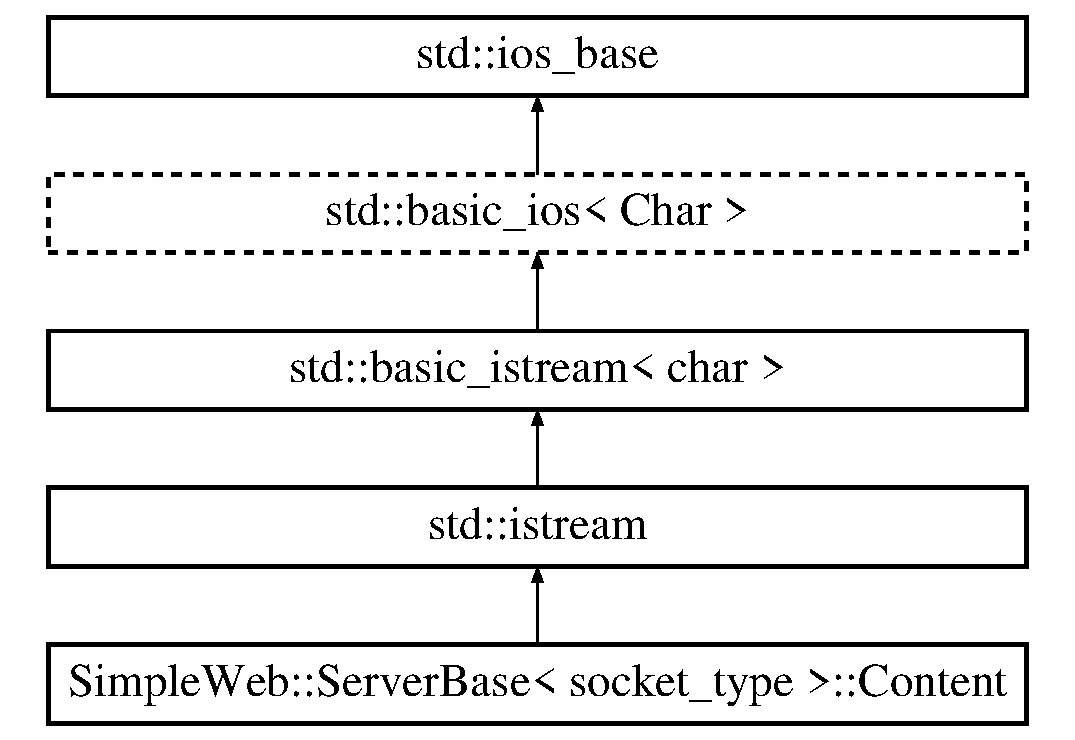
\includegraphics[height=5.000000cm]{a01944}
\end{center}
\end{figure}
\subsection*{Public Member Functions}
\begin{DoxyCompactItemize}
\item 
\mbox{\Hypertarget{a01944_adf8b2386c8ab32277341c6ae07cd4670}\label{a01944_adf8b2386c8ab32277341c6ae07cd4670}} 
size\+\_\+t {\bfseries size} ()
\item 
\mbox{\Hypertarget{a01944_a6b4a72b0631c88ef576db28f54a768cb}\label{a01944_a6b4a72b0631c88ef576db28f54a768cb}} 
std\+::string {\bfseries string} ()
\end{DoxyCompactItemize}
\subsection*{Friends}
\begin{DoxyCompactItemize}
\item 
\mbox{\Hypertarget{a01944_a01d54a7e16ca437c98ec571deca98dfc}\label{a01944_a01d54a7e16ca437c98ec571deca98dfc}} 
class {\bfseries Server\+Base$<$ socket\+\_\+type $>$}
\end{DoxyCompactItemize}


The documentation for this class was generated from the following file\+:\begin{DoxyCompactItemize}
\item 
server\+\_\+http.\+hpp\end{DoxyCompactItemize}

\hypertarget{a01876}{}\section{C\+Simple\+Ini\+Templ$<$ S\+I\+\_\+\+C\+H\+AR, S\+I\+\_\+\+S\+T\+R\+L\+E\+SS, S\+I\+\_\+\+C\+O\+N\+V\+E\+R\+T\+ER $>$\+:\+:Converter Class Reference}
\label{a01876}\index{C\+Simple\+Ini\+Templ$<$ S\+I\+\_\+\+C\+H\+A\+R, S\+I\+\_\+\+S\+T\+R\+L\+E\+S\+S, S\+I\+\_\+\+C\+O\+N\+V\+E\+R\+T\+E\+R $>$\+::\+Converter@{C\+Simple\+Ini\+Templ$<$ S\+I\+\_\+\+C\+H\+A\+R, S\+I\+\_\+\+S\+T\+R\+L\+E\+S\+S, S\+I\+\_\+\+C\+O\+N\+V\+E\+R\+T\+E\+R $>$\+::\+Converter}}


{\ttfamily \#include $<$Simple\+Ini.\+h$>$}

Inheritance diagram for C\+Simple\+Ini\+Templ$<$ S\+I\+\_\+\+C\+H\+AR, S\+I\+\_\+\+S\+T\+R\+L\+E\+SS, S\+I\+\_\+\+C\+O\+N\+V\+E\+R\+T\+ER $>$\+:\+:Converter\+:\begin{figure}[H]
\begin{center}
\leavevmode
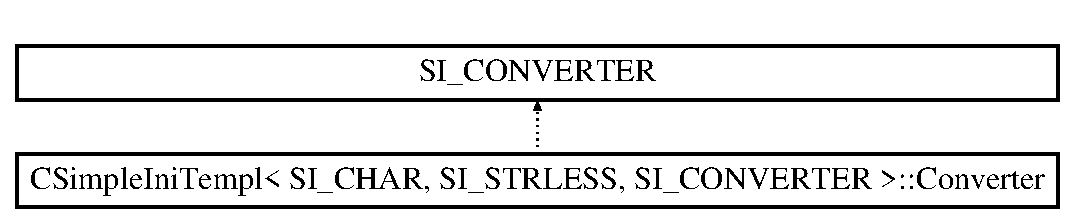
\includegraphics[height=2.000000cm]{a01876}
\end{center}
\end{figure}
\subsection*{Public Member Functions}
\begin{DoxyCompactItemize}
\item 
\mbox{\Hypertarget{a01876_ab8e740b211e4ece127d4d25773ba7e42}\label{a01876_ab8e740b211e4ece127d4d25773ba7e42}} 
{\bfseries Converter} (bool a\+\_\+b\+Store\+Is\+Utf8)
\item 
\mbox{\Hypertarget{a01876_a2f6e993014ed5d60c6e890e55beb0805}\label{a01876_a2f6e993014ed5d60c6e890e55beb0805}} 
{\bfseries Converter} (const \hyperlink{a01876}{Converter} \&rhs)
\item 
\mbox{\Hypertarget{a01876_af858c01c6a7e4ce9fafd18abc9e0ac1b}\label{a01876_af858c01c6a7e4ce9fafd18abc9e0ac1b}} 
\hyperlink{a01876}{Converter} \& {\bfseries operator=} (const \hyperlink{a01876}{Converter} \&rhs)
\item 
\mbox{\Hypertarget{a01876_a4e4186867214b54326cf622e323c9f2f}\label{a01876_a4e4186867214b54326cf622e323c9f2f}} 
bool {\bfseries Convert\+To\+Store} (const S\+I\+\_\+\+C\+H\+AR $\ast$a\+\_\+psz\+String)
\item 
\mbox{\Hypertarget{a01876_a918bbd4f861a2872e148bc9481ac80bb}\label{a01876_a918bbd4f861a2872e148bc9481ac80bb}} 
const char $\ast$ {\bfseries Data} ()
\end{DoxyCompactItemize}


\subsection{Detailed Description}
\subsubsection*{template$<$class S\+I\+\_\+\+C\+H\+AR, class S\+I\+\_\+\+S\+T\+R\+L\+E\+SS, class S\+I\+\_\+\+C\+O\+N\+V\+E\+R\+T\+ER$>$\newline
class C\+Simple\+Ini\+Templ$<$ S\+I\+\_\+\+C\+H\+A\+R, S\+I\+\_\+\+S\+T\+R\+L\+E\+S\+S, S\+I\+\_\+\+C\+O\+N\+V\+E\+R\+T\+E\+R $>$\+::\+Converter}

Characterset conversion utility class to convert strings to the same format as is used for the storage. 

The documentation for this class was generated from the following file\+:\begin{DoxyCompactItemize}
\item 
Simple\+Ini.\+h\end{DoxyCompactItemize}

\hypertarget{a01220}{}\section{Fake\+Vertex\+Four\+Properties Class Reference}
\label{a01220}\index{Fake\+Vertex\+Four\+Properties@{Fake\+Vertex\+Four\+Properties}}
Inheritance diagram for Fake\+Vertex\+Four\+Properties\+:\begin{figure}[H]
\begin{center}
\leavevmode
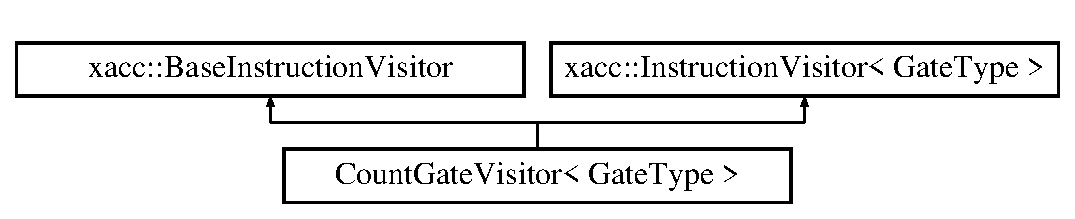
\includegraphics[height=2.000000cm]{a01220}
\end{center}
\end{figure}
\subsection*{Additional Inherited Members}


The documentation for this class was generated from the following file\+:\begin{DoxyCompactItemize}
\item 
Graph\+Tester.\+cpp\end{DoxyCompactItemize}

\hypertarget{a01980}{}\section{Crt\+Allocator Class Reference}
\label{a01980}\index{Crt\+Allocator@{Crt\+Allocator}}


C-\/runtime library allocator.  




{\ttfamily \#include $<$allocators.\+h$>$}

\subsection*{Public Member Functions}
\begin{DoxyCompactItemize}
\item 
\mbox{\Hypertarget{a01980_acd720631f8c094041afa6c7951f0d935}\label{a01980_acd720631f8c094041afa6c7951f0d935}} 
void $\ast$ {\bfseries Malloc} (size\+\_\+t size)
\item 
\mbox{\Hypertarget{a01980_a646bb6f68afe773a62a22f7f14f83e97}\label{a01980_a646bb6f68afe773a62a22f7f14f83e97}} 
void $\ast$ {\bfseries Realloc} (void $\ast$original\+Ptr, size\+\_\+t original\+Size, size\+\_\+t new\+Size)
\end{DoxyCompactItemize}
\subsection*{Static Public Member Functions}
\begin{DoxyCompactItemize}
\item 
\mbox{\Hypertarget{a01980_a5043907058d906dcb1291e9491560373}\label{a01980_a5043907058d906dcb1291e9491560373}} 
static void {\bfseries Free} (void $\ast$ptr)
\end{DoxyCompactItemize}
\subsection*{Static Public Attributes}
\begin{DoxyCompactItemize}
\item 
\mbox{\Hypertarget{a01980_ac7df8398c529290f0cd5950d9492f524}\label{a01980_ac7df8398c529290f0cd5950d9492f524}} 
static const bool {\bfseries k\+Need\+Free} = true
\end{DoxyCompactItemize}


\subsection{Detailed Description}
C-\/runtime library allocator. 

This class is just wrapper for standard C library memory routines. \begin{DoxyNote}{Note}
implements Allocator concept 
\end{DoxyNote}


The documentation for this class was generated from the following file\+:\begin{DoxyCompactItemize}
\item 
allocators.\+h\end{DoxyCompactItemize}

\hypertarget{a01848}{}\section{C\+Simple\+Ini\+Templ$<$ S\+I\+\_\+\+C\+H\+AR, S\+I\+\_\+\+S\+T\+R\+L\+E\+SS, S\+I\+\_\+\+C\+O\+N\+V\+E\+R\+T\+ER $>$ Class Template Reference}
\label{a01848}\index{C\+Simple\+Ini\+Templ$<$ S\+I\+\_\+\+C\+H\+A\+R, S\+I\+\_\+\+S\+T\+R\+L\+E\+S\+S, S\+I\+\_\+\+C\+O\+N\+V\+E\+R\+T\+E\+R $>$@{C\+Simple\+Ini\+Templ$<$ S\+I\+\_\+\+C\+H\+A\+R, S\+I\+\_\+\+S\+T\+R\+L\+E\+S\+S, S\+I\+\_\+\+C\+O\+N\+V\+E\+R\+T\+E\+R $>$}}


{\ttfamily \#include $<$Simple\+Ini.\+h$>$}

\subsection*{Classes}
\begin{DoxyCompactItemize}
\item 
class \hyperlink{a01876}{Converter}
\item 
struct \hyperlink{a01852}{Entry}
\item 
class \hyperlink{a01868}{File\+Writer}
\item 
class \hyperlink{a01864}{Output\+Writer}
\item 
class \hyperlink{a01872}{String\+Writer}
\end{DoxyCompactItemize}
\subsection*{Public Types}
\begin{DoxyCompactItemize}
\item 
\mbox{\Hypertarget{a01848_ad7ffad7e87da2303a05b885e95bc74fa}\label{a01848_ad7ffad7e87da2303a05b885e95bc74fa}} 
typedef S\+I\+\_\+\+C\+H\+AR {\bfseries S\+I\+\_\+\+C\+H\+A\+R\+\_\+T}
\item 
typedef std\+::multimap$<$ \hyperlink{a01852}{Entry}, const S\+I\+\_\+\+C\+H\+AR $\ast$, typename \hyperlink{a01856}{Entry\+::\+Key\+Order} $>$ \hyperlink{a01848_ae7f0e11d84617214bd479de6332c80e6}{T\+Key\+Val}
\item 
typedef std\+::map$<$ \hyperlink{a01852}{Entry}, \hyperlink{a01848_ae7f0e11d84617214bd479de6332c80e6}{T\+Key\+Val}, typename \hyperlink{a01856}{Entry\+::\+Key\+Order} $>$ \hyperlink{a01848_a2e7963455f680abd0d6901786495a665}{T\+Section}
\item 
typedef std\+::list$<$ \hyperlink{a01852}{Entry} $>$ \hyperlink{a01848_a391b3f3751e06cd9e9de4fb16ac14342}{T\+Names\+Depend}
\end{DoxyCompactItemize}
\subsection*{Public Member Functions}
\begin{DoxyCompactItemize}
\item 
\hyperlink{a01848_af878d0a2aa780255b621e95f58f691d8}{C\+Simple\+Ini\+Templ} (bool a\+\_\+b\+Is\+Utf8=false, bool a\+\_\+b\+Multi\+Key=false, bool a\+\_\+b\+Multi\+Line=false)
\item 
\hyperlink{a01848_a8c933adc1d46bb663caeb6f9dee5aa12}{$\sim$\+C\+Simple\+Ini\+Templ} ()
\item 
void \hyperlink{a01848_a89b34d38be4518e9ed91c634a41b8055}{Reset} ()
\item 
bool \hyperlink{a01848_a54bbe9727db17b368a0a75abd5e52d1c}{Is\+Empty} () const
\item 
S\+I\+\_\+\+Error \hyperlink{a01848_aebb6e5fff76efc05ca6cc4b7b56481a3}{Load\+File} (const char $\ast$a\+\_\+psz\+File)
\item 
S\+I\+\_\+\+Error \hyperlink{a01848_a7ccb65e82fa347b42b59330968f826ae}{Load\+File} (F\+I\+LE $\ast$a\+\_\+fp\+File)
\item 
S\+I\+\_\+\+Error \hyperlink{a01848_a174244fd3e09ff78da05fe46be86e714}{Load\+Data} (const std\+::string \&a\+\_\+str\+Data)
\item 
S\+I\+\_\+\+Error \hyperlink{a01848_aa797cf47cec05906f07d5065882af4d3}{Load\+Data} (const char $\ast$a\+\_\+p\+Data, size\+\_\+t a\+\_\+u\+Data\+Len)
\item 
S\+I\+\_\+\+Error \hyperlink{a01848_af00e754689a94cbe87b387f99f7a5d01}{Save\+File} (const char $\ast$a\+\_\+psz\+File, bool a\+\_\+b\+Add\+Signature=true) const
\item 
S\+I\+\_\+\+Error \hyperlink{a01848_a3c3f677c1515e08751cb52a1dfaf1a93}{Save\+File} (F\+I\+LE $\ast$a\+\_\+p\+File, bool a\+\_\+b\+Add\+Signature=false) const
\item 
S\+I\+\_\+\+Error \hyperlink{a01848_a6ec10daab297e92cdffe024ba5e6d999}{Save} (\hyperlink{a01864}{Output\+Writer} \&a\+\_\+o\+Output, bool a\+\_\+b\+Add\+Signature=false) const
\item 
S\+I\+\_\+\+Error \hyperlink{a01848_a9fc5894f12a31b8496a9627cd0f42139}{Save} (std\+::string \&a\+\_\+s\+Buffer, bool a\+\_\+b\+Add\+Signature=false) const
\item 
void \hyperlink{a01848_a7fe8a8b70b0ef000c591011a8332ebd5}{Get\+All\+Sections} (\hyperlink{a01848_a391b3f3751e06cd9e9de4fb16ac14342}{T\+Names\+Depend} \&a\+\_\+names) const
\item 
bool \hyperlink{a01848_a08cadb6624a6c459703efaadb25d31c9}{Get\+All\+Keys} (const S\+I\+\_\+\+C\+H\+AR $\ast$a\+\_\+p\+Section, \hyperlink{a01848_a391b3f3751e06cd9e9de4fb16ac14342}{T\+Names\+Depend} \&a\+\_\+names) const
\item 
bool \hyperlink{a01848_adda5ee7f422695f7e67be2d066e303bf}{Get\+All\+Values} (const S\+I\+\_\+\+C\+H\+AR $\ast$a\+\_\+p\+Section, const S\+I\+\_\+\+C\+H\+AR $\ast$a\+\_\+p\+Key, \hyperlink{a01848_a391b3f3751e06cd9e9de4fb16ac14342}{T\+Names\+Depend} \&a\+\_\+values) const
\item 
int \hyperlink{a01848_a0a9c089eabb5faf764c4af449f7b1846}{Get\+Section\+Size} (const S\+I\+\_\+\+C\+H\+AR $\ast$a\+\_\+p\+Section) const
\item 
const \hyperlink{a01848_ae7f0e11d84617214bd479de6332c80e6}{T\+Key\+Val} $\ast$ \hyperlink{a01848_a56a6838556328ab8bfaa7ded9edb9c8a}{Get\+Section} (const S\+I\+\_\+\+C\+H\+AR $\ast$a\+\_\+p\+Section) const
\item 
const S\+I\+\_\+\+C\+H\+AR $\ast$ \hyperlink{a01848_a74e3f5d22f50b70b2a20c89ec7e2c737}{Get\+Value} (const S\+I\+\_\+\+C\+H\+AR $\ast$a\+\_\+p\+Section, const S\+I\+\_\+\+C\+H\+AR $\ast$a\+\_\+p\+Key, const S\+I\+\_\+\+C\+H\+AR $\ast$a\+\_\+p\+Default=N\+U\+LL, bool $\ast$a\+\_\+p\+Has\+Multiple=N\+U\+LL) const
\item 
long \hyperlink{a01848_a7fa211c1c768497520eab7f2014ae786}{Get\+Long\+Value} (const S\+I\+\_\+\+C\+H\+AR $\ast$a\+\_\+p\+Section, const S\+I\+\_\+\+C\+H\+AR $\ast$a\+\_\+p\+Key, long a\+\_\+n\+Default=0, bool $\ast$a\+\_\+p\+Has\+Multiple=N\+U\+LL) const
\item 
double \hyperlink{a01848_aab58a949481926cf1d42fcbf9552d77b}{Get\+Double\+Value} (const S\+I\+\_\+\+C\+H\+AR $\ast$a\+\_\+p\+Section, const S\+I\+\_\+\+C\+H\+AR $\ast$a\+\_\+p\+Key, double a\+\_\+n\+Default=0, bool $\ast$a\+\_\+p\+Has\+Multiple=N\+U\+LL) const
\item 
bool \hyperlink{a01848_a76b3165ce01224f82daee5ef63b3c96d}{Get\+Bool\+Value} (const S\+I\+\_\+\+C\+H\+AR $\ast$a\+\_\+p\+Section, const S\+I\+\_\+\+C\+H\+AR $\ast$a\+\_\+p\+Key, bool a\+\_\+b\+Default=false, bool $\ast$a\+\_\+p\+Has\+Multiple=N\+U\+LL) const
\item 
S\+I\+\_\+\+Error \hyperlink{a01848_aa2014a3dc8fdd638316cf1d3611796ab}{Set\+Value} (const S\+I\+\_\+\+C\+H\+AR $\ast$a\+\_\+p\+Section, const S\+I\+\_\+\+C\+H\+AR $\ast$a\+\_\+p\+Key, const S\+I\+\_\+\+C\+H\+AR $\ast$a\+\_\+p\+Value, const S\+I\+\_\+\+C\+H\+AR $\ast$a\+\_\+p\+Comment=N\+U\+LL, bool a\+\_\+b\+Force\+Replace=false)
\item 
S\+I\+\_\+\+Error \hyperlink{a01848_ab2238be407232e4bba0f1343e4793e4e}{Set\+Long\+Value} (const S\+I\+\_\+\+C\+H\+AR $\ast$a\+\_\+p\+Section, const S\+I\+\_\+\+C\+H\+AR $\ast$a\+\_\+p\+Key, long a\+\_\+n\+Value, const S\+I\+\_\+\+C\+H\+AR $\ast$a\+\_\+p\+Comment=N\+U\+LL, bool a\+\_\+b\+Use\+Hex=false, bool a\+\_\+b\+Force\+Replace=false)
\item 
S\+I\+\_\+\+Error \hyperlink{a01848_af92ba0b8067553ab693c62a370de6534}{Set\+Double\+Value} (const S\+I\+\_\+\+C\+H\+AR $\ast$a\+\_\+p\+Section, const S\+I\+\_\+\+C\+H\+AR $\ast$a\+\_\+p\+Key, double a\+\_\+n\+Value, const S\+I\+\_\+\+C\+H\+AR $\ast$a\+\_\+p\+Comment=N\+U\+LL, bool a\+\_\+b\+Force\+Replace=false)
\item 
S\+I\+\_\+\+Error \hyperlink{a01848_a48ae136fa20c5d7eb7ab0b75342b27cf}{Set\+Bool\+Value} (const S\+I\+\_\+\+C\+H\+AR $\ast$a\+\_\+p\+Section, const S\+I\+\_\+\+C\+H\+AR $\ast$a\+\_\+p\+Key, bool a\+\_\+b\+Value, const S\+I\+\_\+\+C\+H\+AR $\ast$a\+\_\+p\+Comment=N\+U\+LL, bool a\+\_\+b\+Force\+Replace=false)
\item 
bool \hyperlink{a01848_aa5c1cdd0b306434d9e9f1422888049da}{Delete} (const S\+I\+\_\+\+C\+H\+AR $\ast$a\+\_\+p\+Section, const S\+I\+\_\+\+C\+H\+AR $\ast$a\+\_\+p\+Key, bool a\+\_\+b\+Remove\+Empty=false)
\item 
\hyperlink{a01876}{Converter} \hyperlink{a01848_a4a48496d4e4840a2254a9e31e16eaf6d}{Get\+Converter} () const
\end{DoxyCompactItemize}
\begin{Indent}\textbf{ Settings}\par
\begin{DoxyCompactItemize}
\item 
void \hyperlink{a01848_aa9a15a66de893571014f661f89cb4d4b}{Set\+Unicode} (bool a\+\_\+b\+Is\+Utf8=true)
\item 
bool \hyperlink{a01848_a40b4ee04251bd343ada5c4a4c508cd43}{Is\+Unicode} () const
\item 
void \hyperlink{a01848_ac3cfaf072a64f960bdcb7ddf2edc52b6}{Set\+Multi\+Key} (bool a\+\_\+b\+Allow\+Multi\+Key=true)
\item 
bool \hyperlink{a01848_a494b30fbdda5e78afdb25451743df935}{Is\+Multi\+Key} () const
\item 
void \hyperlink{a01848_aa7214b76600790053a5c715e9730aab0}{Set\+Multi\+Line} (bool a\+\_\+b\+Allow\+Multi\+Line=true)
\item 
bool \hyperlink{a01848_afadd3818363ec7e66ca369ef486ec979}{Is\+Multi\+Line} () const
\item 
void \hyperlink{a01848_ae3c0eae2dcd84a42c99bb86ae103662c}{Set\+Spaces} (bool a\+\_\+b\+Spaces=true)
\item 
bool \hyperlink{a01848_a92203e0c21f8d71e5d1621a18ee0be50}{Using\+Spaces} () const
\end{DoxyCompactItemize}
\end{Indent}


\subsection{Detailed Description}
\subsubsection*{template$<$class S\+I\+\_\+\+C\+H\+AR, class S\+I\+\_\+\+S\+T\+R\+L\+E\+SS, class S\+I\+\_\+\+C\+O\+N\+V\+E\+R\+T\+ER$>$\newline
class C\+Simple\+Ini\+Templ$<$ S\+I\+\_\+\+C\+H\+A\+R, S\+I\+\_\+\+S\+T\+R\+L\+E\+S\+S, S\+I\+\_\+\+C\+O\+N\+V\+E\+R\+T\+E\+R $>$}

Simple I\+NI file reader.

This can be instantiated with the choice of unicode or native characterset, and case sensitive or insensitive comparisons of section and key names. The supported combinations are pre-\/defined with the following typedefs\+:

\tabulinesep=1mm
\begin{longtabu} spread 0pt [c]{*{3}{|X[-1]}|}
\hline
\rowcolor{\tableheadbgcolor}\textbf{ Interface }&\textbf{ Case-\/sensitive }&\textbf{ Typedef }\\\cline{1-3}
\endfirsthead
\hline
\endfoot
\hline
\rowcolor{\tableheadbgcolor}\textbf{ Interface }&\textbf{ Case-\/sensitive }&\textbf{ Typedef }\\\cline{1-3}
\endhead
char &No &C\+Simple\+IniA \\\cline{1-3}
char &Yes &C\+Simple\+Ini\+CaseA \\\cline{1-3}
wchar\+\_\+t &No &C\+Simple\+IniW \\\cline{1-3}
wchar\+\_\+t &Yes &C\+Simple\+Ini\+CaseW \\\cline{1-3}
\end{longtabu}


Note that using other types for the S\+I\+\_\+\+C\+H\+AR is supported. For instance, unsigned char, unsigned short, etc. Note that where the alternative type is a different size to char/wchar\+\_\+t you may need to supply new helper classes for S\+I\+\_\+\+S\+T\+R\+L\+E\+SS and S\+I\+\_\+\+C\+O\+N\+V\+E\+R\+T\+ER. 

\subsection{Member Typedef Documentation}
\mbox{\Hypertarget{a01848_ae7f0e11d84617214bd479de6332c80e6}\label{a01848_ae7f0e11d84617214bd479de6332c80e6}} 
\index{C\+Simple\+Ini\+Templ@{C\+Simple\+Ini\+Templ}!T\+Key\+Val@{T\+Key\+Val}}
\index{T\+Key\+Val@{T\+Key\+Val}!C\+Simple\+Ini\+Templ@{C\+Simple\+Ini\+Templ}}
\subsubsection{\texorpdfstring{T\+Key\+Val}{TKeyVal}}
{\footnotesize\ttfamily template$<$class S\+I\+\_\+\+C\+H\+AR , class S\+I\+\_\+\+S\+T\+R\+L\+E\+SS , class S\+I\+\_\+\+C\+O\+N\+V\+E\+R\+T\+ER $>$ \\
typedef std\+::multimap$<$\hyperlink{a01852}{Entry},const S\+I\+\_\+\+C\+H\+AR $\ast$,typename \hyperlink{a01856}{Entry\+::\+Key\+Order}$>$ \hyperlink{a01848}{C\+Simple\+Ini\+Templ}$<$ S\+I\+\_\+\+C\+H\+AR, S\+I\+\_\+\+S\+T\+R\+L\+E\+SS, S\+I\+\_\+\+C\+O\+N\+V\+E\+R\+T\+ER $>$\+::\hyperlink{a01848_ae7f0e11d84617214bd479de6332c80e6}{T\+Key\+Val}}

map keys to values \mbox{\Hypertarget{a01848_a391b3f3751e06cd9e9de4fb16ac14342}\label{a01848_a391b3f3751e06cd9e9de4fb16ac14342}} 
\index{C\+Simple\+Ini\+Templ@{C\+Simple\+Ini\+Templ}!T\+Names\+Depend@{T\+Names\+Depend}}
\index{T\+Names\+Depend@{T\+Names\+Depend}!C\+Simple\+Ini\+Templ@{C\+Simple\+Ini\+Templ}}
\subsubsection{\texorpdfstring{T\+Names\+Depend}{TNamesDepend}}
{\footnotesize\ttfamily template$<$class S\+I\+\_\+\+C\+H\+AR , class S\+I\+\_\+\+S\+T\+R\+L\+E\+SS , class S\+I\+\_\+\+C\+O\+N\+V\+E\+R\+T\+ER $>$ \\
typedef std\+::list$<$\hyperlink{a01852}{Entry}$>$ \hyperlink{a01848}{C\+Simple\+Ini\+Templ}$<$ S\+I\+\_\+\+C\+H\+AR, S\+I\+\_\+\+S\+T\+R\+L\+E\+SS, S\+I\+\_\+\+C\+O\+N\+V\+E\+R\+T\+ER $>$\+::\hyperlink{a01848_a391b3f3751e06cd9e9de4fb16ac14342}{T\+Names\+Depend}}

set of dependent string pointers. Note that these pointers are dependent on memory owned by C\+Simple\+Ini. \mbox{\Hypertarget{a01848_a2e7963455f680abd0d6901786495a665}\label{a01848_a2e7963455f680abd0d6901786495a665}} 
\index{C\+Simple\+Ini\+Templ@{C\+Simple\+Ini\+Templ}!T\+Section@{T\+Section}}
\index{T\+Section@{T\+Section}!C\+Simple\+Ini\+Templ@{C\+Simple\+Ini\+Templ}}
\subsubsection{\texorpdfstring{T\+Section}{TSection}}
{\footnotesize\ttfamily template$<$class S\+I\+\_\+\+C\+H\+AR , class S\+I\+\_\+\+S\+T\+R\+L\+E\+SS , class S\+I\+\_\+\+C\+O\+N\+V\+E\+R\+T\+ER $>$ \\
typedef std\+::map$<$\hyperlink{a01852}{Entry},\hyperlink{a01848_ae7f0e11d84617214bd479de6332c80e6}{T\+Key\+Val},typename \hyperlink{a01856}{Entry\+::\+Key\+Order}$>$ \hyperlink{a01848}{C\+Simple\+Ini\+Templ}$<$ S\+I\+\_\+\+C\+H\+AR, S\+I\+\_\+\+S\+T\+R\+L\+E\+SS, S\+I\+\_\+\+C\+O\+N\+V\+E\+R\+T\+ER $>$\+::\hyperlink{a01848_a2e7963455f680abd0d6901786495a665}{T\+Section}}

map sections to key/value map 

\subsection{Constructor \& Destructor Documentation}
\mbox{\Hypertarget{a01848_af878d0a2aa780255b621e95f58f691d8}\label{a01848_af878d0a2aa780255b621e95f58f691d8}} 
\index{C\+Simple\+Ini\+Templ@{C\+Simple\+Ini\+Templ}!C\+Simple\+Ini\+Templ@{C\+Simple\+Ini\+Templ}}
\index{C\+Simple\+Ini\+Templ@{C\+Simple\+Ini\+Templ}!C\+Simple\+Ini\+Templ@{C\+Simple\+Ini\+Templ}}
\subsubsection{\texorpdfstring{C\+Simple\+Ini\+Templ()}{CSimpleIniTempl()}}
{\footnotesize\ttfamily template$<$class S\+I\+\_\+\+C\+H\+AR , class S\+I\+\_\+\+S\+T\+R\+L\+E\+SS , class S\+I\+\_\+\+C\+O\+N\+V\+E\+R\+T\+ER $>$ \\
\hyperlink{a01848}{C\+Simple\+Ini\+Templ}$<$ S\+I\+\_\+\+C\+H\+AR, S\+I\+\_\+\+S\+T\+R\+L\+E\+SS, S\+I\+\_\+\+C\+O\+N\+V\+E\+R\+T\+ER $>$\+::\hyperlink{a01848}{C\+Simple\+Ini\+Templ} (\begin{DoxyParamCaption}\item[{bool}]{a\+\_\+b\+Is\+Utf8 = {\ttfamily false},  }\item[{bool}]{a\+\_\+b\+Multi\+Key = {\ttfamily false},  }\item[{bool}]{a\+\_\+b\+Multi\+Line = {\ttfamily false} }\end{DoxyParamCaption})}

Default constructor.


\begin{DoxyParams}{Parameters}
{\em a\+\_\+b\+Is\+Utf8} & See the method \hyperlink{a01848_aa9a15a66de893571014f661f89cb4d4b}{Set\+Unicode()} for details. \\
\hline
{\em a\+\_\+b\+Multi\+Key} & See the method \hyperlink{a01848_ac3cfaf072a64f960bdcb7ddf2edc52b6}{Set\+Multi\+Key()} for details. \\
\hline
{\em a\+\_\+b\+Multi\+Line} & See the method \hyperlink{a01848_aa7214b76600790053a5c715e9730aab0}{Set\+Multi\+Line()} for details. \\
\hline
\end{DoxyParams}
\mbox{\Hypertarget{a01848_a8c933adc1d46bb663caeb6f9dee5aa12}\label{a01848_a8c933adc1d46bb663caeb6f9dee5aa12}} 
\index{C\+Simple\+Ini\+Templ@{C\+Simple\+Ini\+Templ}!````~C\+Simple\+Ini\+Templ@{$\sim$\+C\+Simple\+Ini\+Templ}}
\index{````~C\+Simple\+Ini\+Templ@{$\sim$\+C\+Simple\+Ini\+Templ}!C\+Simple\+Ini\+Templ@{C\+Simple\+Ini\+Templ}}
\subsubsection{\texorpdfstring{$\sim$\+C\+Simple\+Ini\+Templ()}{~CSimpleIniTempl()}}
{\footnotesize\ttfamily template$<$class S\+I\+\_\+\+C\+H\+AR , class S\+I\+\_\+\+S\+T\+R\+L\+E\+SS , class S\+I\+\_\+\+C\+O\+N\+V\+E\+R\+T\+ER $>$ \\
\hyperlink{a01848}{C\+Simple\+Ini\+Templ}$<$ S\+I\+\_\+\+C\+H\+AR, S\+I\+\_\+\+S\+T\+R\+L\+E\+SS, S\+I\+\_\+\+C\+O\+N\+V\+E\+R\+T\+ER $>$\+::$\sim$\hyperlink{a01848}{C\+Simple\+Ini\+Templ} (\begin{DoxyParamCaption}{ }\end{DoxyParamCaption})}

Destructor 

\subsection{Member Function Documentation}
\mbox{\Hypertarget{a01848_aa5c1cdd0b306434d9e9f1422888049da}\label{a01848_aa5c1cdd0b306434d9e9f1422888049da}} 
\index{C\+Simple\+Ini\+Templ@{C\+Simple\+Ini\+Templ}!Delete@{Delete}}
\index{Delete@{Delete}!C\+Simple\+Ini\+Templ@{C\+Simple\+Ini\+Templ}}
\subsubsection{\texorpdfstring{Delete()}{Delete()}}
{\footnotesize\ttfamily template$<$class S\+I\+\_\+\+C\+H\+AR , class S\+I\+\_\+\+S\+T\+R\+L\+E\+SS , class S\+I\+\_\+\+C\+O\+N\+V\+E\+R\+T\+ER $>$ \\
bool \hyperlink{a01848}{C\+Simple\+Ini\+Templ}$<$ S\+I\+\_\+\+C\+H\+AR, S\+I\+\_\+\+S\+T\+R\+L\+E\+SS, S\+I\+\_\+\+C\+O\+N\+V\+E\+R\+T\+ER $>$\+::Delete (\begin{DoxyParamCaption}\item[{const S\+I\+\_\+\+C\+H\+AR $\ast$}]{a\+\_\+p\+Section,  }\item[{const S\+I\+\_\+\+C\+H\+AR $\ast$}]{a\+\_\+p\+Key,  }\item[{bool}]{a\+\_\+b\+Remove\+Empty = {\ttfamily false} }\end{DoxyParamCaption})}

Delete an entire section, or a key from a section. Note that the data returned by Get\+Section is invalid and must not be used after anything has been deleted from that section using this method. Note when multiple keys is enabled, this will delete all keys with that name; there is no way to selectively delete individual key/values in this situation.


\begin{DoxyParams}{Parameters}
{\em a\+\_\+p\+Section} & Section to delete key from, or if a\+\_\+p\+Key is N\+U\+LL, the section to remove. \\
\hline
{\em a\+\_\+p\+Key} & Key to remove from the section. Set to N\+U\+LL to remove the entire section. \\
\hline
{\em a\+\_\+b\+Remove\+Empty} & If the section is empty after this key has been deleted, should the empty section be removed?\\
\hline
\end{DoxyParams}
\begin{DoxyReturn}{Returns}
true Key or section was deleted. 

false Key or section was not found. 
\end{DoxyReturn}
\mbox{\Hypertarget{a01848_a08cadb6624a6c459703efaadb25d31c9}\label{a01848_a08cadb6624a6c459703efaadb25d31c9}} 
\index{C\+Simple\+Ini\+Templ@{C\+Simple\+Ini\+Templ}!Get\+All\+Keys@{Get\+All\+Keys}}
\index{Get\+All\+Keys@{Get\+All\+Keys}!C\+Simple\+Ini\+Templ@{C\+Simple\+Ini\+Templ}}
\subsubsection{\texorpdfstring{Get\+All\+Keys()}{GetAllKeys()}}
{\footnotesize\ttfamily template$<$class S\+I\+\_\+\+C\+H\+AR , class S\+I\+\_\+\+S\+T\+R\+L\+E\+SS , class S\+I\+\_\+\+C\+O\+N\+V\+E\+R\+T\+ER $>$ \\
bool \hyperlink{a01848}{C\+Simple\+Ini\+Templ}$<$ S\+I\+\_\+\+C\+H\+AR, S\+I\+\_\+\+S\+T\+R\+L\+E\+SS, S\+I\+\_\+\+C\+O\+N\+V\+E\+R\+T\+ER $>$\+::Get\+All\+Keys (\begin{DoxyParamCaption}\item[{const S\+I\+\_\+\+C\+H\+AR $\ast$}]{a\+\_\+p\+Section,  }\item[{\hyperlink{a01848_a391b3f3751e06cd9e9de4fb16ac14342}{T\+Names\+Depend} \&}]{a\+\_\+names }\end{DoxyParamCaption}) const}

Retrieve all unique key names in a section. The sort order of the returned strings is N\+OT D\+E\+F\+I\+N\+ED. You can sort the names into the load order if desired. Search this file for \char`\"{}.\+sort\char`\"{} for an example. Only unique key names are returned.

N\+O\+T\+E! This structure contains only pointers to strings. The actual string data is stored in memory owned by C\+Simple\+Ini. Ensure that the C\+Simple\+Ini object is not destroyed or \hyperlink{a01848_a89b34d38be4518e9ed91c634a41b8055}{Reset()} while these strings are in use!


\begin{DoxyParams}{Parameters}
{\em a\+\_\+p\+Section} & Section to request data for \\
\hline
{\em a\+\_\+names} & List that will receive all of the key names. See note above!\\
\hline
\end{DoxyParams}
\begin{DoxyReturn}{Returns}
true Section was found. 

false Matching section was not found. 
\end{DoxyReturn}
\mbox{\Hypertarget{a01848_a7fe8a8b70b0ef000c591011a8332ebd5}\label{a01848_a7fe8a8b70b0ef000c591011a8332ebd5}} 
\index{C\+Simple\+Ini\+Templ@{C\+Simple\+Ini\+Templ}!Get\+All\+Sections@{Get\+All\+Sections}}
\index{Get\+All\+Sections@{Get\+All\+Sections}!C\+Simple\+Ini\+Templ@{C\+Simple\+Ini\+Templ}}
\subsubsection{\texorpdfstring{Get\+All\+Sections()}{GetAllSections()}}
{\footnotesize\ttfamily template$<$class S\+I\+\_\+\+C\+H\+AR , class S\+I\+\_\+\+S\+T\+R\+L\+E\+SS , class S\+I\+\_\+\+C\+O\+N\+V\+E\+R\+T\+ER $>$ \\
void \hyperlink{a01848}{C\+Simple\+Ini\+Templ}$<$ S\+I\+\_\+\+C\+H\+AR, S\+I\+\_\+\+S\+T\+R\+L\+E\+SS, S\+I\+\_\+\+C\+O\+N\+V\+E\+R\+T\+ER $>$\+::Get\+All\+Sections (\begin{DoxyParamCaption}\item[{\hyperlink{a01848_a391b3f3751e06cd9e9de4fb16ac14342}{T\+Names\+Depend} \&}]{a\+\_\+names }\end{DoxyParamCaption}) const}

Retrieve all section names. The list is returned as an S\+TL vector of names and can be iterated or searched as necessary. Note that the sort order of the returned strings is N\+OT D\+E\+F\+I\+N\+ED. You can sort the names into the load order if desired. Search this file for \char`\"{}.\+sort\char`\"{} for an example.

N\+O\+T\+E! This structure contains only pointers to strings. The actual string data is stored in memory owned by C\+Simple\+Ini. Ensure that the C\+Simple\+Ini object is not destroyed or \hyperlink{a01848_a89b34d38be4518e9ed91c634a41b8055}{Reset()} while these pointers are in use!


\begin{DoxyParams}{Parameters}
{\em a\+\_\+names} & Vector that will receive all of the section names. See note above! \\
\hline
\end{DoxyParams}
\mbox{\Hypertarget{a01848_adda5ee7f422695f7e67be2d066e303bf}\label{a01848_adda5ee7f422695f7e67be2d066e303bf}} 
\index{C\+Simple\+Ini\+Templ@{C\+Simple\+Ini\+Templ}!Get\+All\+Values@{Get\+All\+Values}}
\index{Get\+All\+Values@{Get\+All\+Values}!C\+Simple\+Ini\+Templ@{C\+Simple\+Ini\+Templ}}
\subsubsection{\texorpdfstring{Get\+All\+Values()}{GetAllValues()}}
{\footnotesize\ttfamily template$<$class S\+I\+\_\+\+C\+H\+AR , class S\+I\+\_\+\+S\+T\+R\+L\+E\+SS , class S\+I\+\_\+\+C\+O\+N\+V\+E\+R\+T\+ER $>$ \\
bool \hyperlink{a01848}{C\+Simple\+Ini\+Templ}$<$ S\+I\+\_\+\+C\+H\+AR, S\+I\+\_\+\+S\+T\+R\+L\+E\+SS, S\+I\+\_\+\+C\+O\+N\+V\+E\+R\+T\+ER $>$\+::Get\+All\+Values (\begin{DoxyParamCaption}\item[{const S\+I\+\_\+\+C\+H\+AR $\ast$}]{a\+\_\+p\+Section,  }\item[{const S\+I\+\_\+\+C\+H\+AR $\ast$}]{a\+\_\+p\+Key,  }\item[{\hyperlink{a01848_a391b3f3751e06cd9e9de4fb16ac14342}{T\+Names\+Depend} \&}]{a\+\_\+values }\end{DoxyParamCaption}) const}

Retrieve all values for a specific key. This method can be used when multiple keys are both enabled and disabled. Note that the sort order of the returned strings is N\+OT D\+E\+F\+I\+N\+ED. You can sort the names into the load order if desired. Search this file for \char`\"{}.\+sort\char`\"{} for an example.

N\+O\+T\+E! The returned values are pointers to string data stored in memory owned by C\+Simple\+Ini. Ensure that the C\+Simple\+Ini object is not destroyed or Reset while you are using this pointer!


\begin{DoxyParams}{Parameters}
{\em a\+\_\+p\+Section} & Section to search \\
\hline
{\em a\+\_\+p\+Key} & Key to search for \\
\hline
{\em a\+\_\+values} & List to return if the key is not found\\
\hline
\end{DoxyParams}
\begin{DoxyReturn}{Returns}
true Key was found. 

false Matching section/key was not found. 
\end{DoxyReturn}
\mbox{\Hypertarget{a01848_a76b3165ce01224f82daee5ef63b3c96d}\label{a01848_a76b3165ce01224f82daee5ef63b3c96d}} 
\index{C\+Simple\+Ini\+Templ@{C\+Simple\+Ini\+Templ}!Get\+Bool\+Value@{Get\+Bool\+Value}}
\index{Get\+Bool\+Value@{Get\+Bool\+Value}!C\+Simple\+Ini\+Templ@{C\+Simple\+Ini\+Templ}}
\subsubsection{\texorpdfstring{Get\+Bool\+Value()}{GetBoolValue()}}
{\footnotesize\ttfamily template$<$class S\+I\+\_\+\+C\+H\+AR , class S\+I\+\_\+\+S\+T\+R\+L\+E\+SS , class S\+I\+\_\+\+C\+O\+N\+V\+E\+R\+T\+ER $>$ \\
bool \hyperlink{a01848}{C\+Simple\+Ini\+Templ}$<$ S\+I\+\_\+\+C\+H\+AR, S\+I\+\_\+\+S\+T\+R\+L\+E\+SS, S\+I\+\_\+\+C\+O\+N\+V\+E\+R\+T\+ER $>$\+::Get\+Bool\+Value (\begin{DoxyParamCaption}\item[{const S\+I\+\_\+\+C\+H\+AR $\ast$}]{a\+\_\+p\+Section,  }\item[{const S\+I\+\_\+\+C\+H\+AR $\ast$}]{a\+\_\+p\+Key,  }\item[{bool}]{a\+\_\+b\+Default = {\ttfamily false},  }\item[{bool $\ast$}]{a\+\_\+p\+Has\+Multiple = {\ttfamily NULL} }\end{DoxyParamCaption}) const}

Retrieve a boolean value for a specific key. If multiple keys are enabled (see Set\+Multi\+Key) then only the first value associated with that key will be returned, see Get\+All\+Values for getting all values with multikey.

Strings starting with \char`\"{}t\char`\"{}, \char`\"{}y\char`\"{}, \char`\"{}on\char`\"{} or \char`\"{}1\char`\"{} are returned as logically true. Strings starting with \char`\"{}f\char`\"{}, \char`\"{}n\char`\"{}, \char`\"{}of\char`\"{} or \char`\"{}0\char`\"{} are returned as logically false. For all other values the default is returned. Character comparisons are case-\/insensitive.


\begin{DoxyParams}{Parameters}
{\em a\+\_\+p\+Section} & Section to search \\
\hline
{\em a\+\_\+p\+Key} & Key to search for \\
\hline
{\em a\+\_\+b\+Default} & Value to return if the key is not found \\
\hline
{\em a\+\_\+p\+Has\+Multiple} & Optionally receive notification of if there are multiple entries for this key.\\
\hline
\end{DoxyParams}
\begin{DoxyReturn}{Returns}
a\+\_\+n\+Default Key was not found in the section 

other Value of the key 
\end{DoxyReturn}
\mbox{\Hypertarget{a01848_a4a48496d4e4840a2254a9e31e16eaf6d}\label{a01848_a4a48496d4e4840a2254a9e31e16eaf6d}} 
\index{C\+Simple\+Ini\+Templ@{C\+Simple\+Ini\+Templ}!Get\+Converter@{Get\+Converter}}
\index{Get\+Converter@{Get\+Converter}!C\+Simple\+Ini\+Templ@{C\+Simple\+Ini\+Templ}}
\subsubsection{\texorpdfstring{Get\+Converter()}{GetConverter()}}
{\footnotesize\ttfamily template$<$class S\+I\+\_\+\+C\+H\+AR , class S\+I\+\_\+\+S\+T\+R\+L\+E\+SS , class S\+I\+\_\+\+C\+O\+N\+V\+E\+R\+T\+ER $>$ \\
\hyperlink{a01876}{Converter} \hyperlink{a01848}{C\+Simple\+Ini\+Templ}$<$ S\+I\+\_\+\+C\+H\+AR, S\+I\+\_\+\+S\+T\+R\+L\+E\+SS, S\+I\+\_\+\+C\+O\+N\+V\+E\+R\+T\+ER $>$\+::Get\+Converter (\begin{DoxyParamCaption}{ }\end{DoxyParamCaption}) const\hspace{0.3cm}{\ttfamily [inline]}}

Return a conversion object to convert text to the same encoding as is used by the \hyperlink{a01848_a6ec10daab297e92cdffe024ba5e6d999}{Save()}, \hyperlink{a01848_af00e754689a94cbe87b387f99f7a5d01}{Save\+File()} and Save\+String() functions. Use this to prepare the strings that you wish to append or prepend to the output I\+NI data. \mbox{\Hypertarget{a01848_aab58a949481926cf1d42fcbf9552d77b}\label{a01848_aab58a949481926cf1d42fcbf9552d77b}} 
\index{C\+Simple\+Ini\+Templ@{C\+Simple\+Ini\+Templ}!Get\+Double\+Value@{Get\+Double\+Value}}
\index{Get\+Double\+Value@{Get\+Double\+Value}!C\+Simple\+Ini\+Templ@{C\+Simple\+Ini\+Templ}}
\subsubsection{\texorpdfstring{Get\+Double\+Value()}{GetDoubleValue()}}
{\footnotesize\ttfamily template$<$class S\+I\+\_\+\+C\+H\+AR , class S\+I\+\_\+\+S\+T\+R\+L\+E\+SS , class S\+I\+\_\+\+C\+O\+N\+V\+E\+R\+T\+ER $>$ \\
double \hyperlink{a01848}{C\+Simple\+Ini\+Templ}$<$ S\+I\+\_\+\+C\+H\+AR, S\+I\+\_\+\+S\+T\+R\+L\+E\+SS, S\+I\+\_\+\+C\+O\+N\+V\+E\+R\+T\+ER $>$\+::Get\+Double\+Value (\begin{DoxyParamCaption}\item[{const S\+I\+\_\+\+C\+H\+AR $\ast$}]{a\+\_\+p\+Section,  }\item[{const S\+I\+\_\+\+C\+H\+AR $\ast$}]{a\+\_\+p\+Key,  }\item[{double}]{a\+\_\+n\+Default = {\ttfamily 0},  }\item[{bool $\ast$}]{a\+\_\+p\+Has\+Multiple = {\ttfamily NULL} }\end{DoxyParamCaption}) const}

Retrieve a numeric value for a specific key. If multiple keys are enabled (see Set\+Multi\+Key) then only the first value associated with that key will be returned, see Get\+All\+Values for getting all values with multikey.


\begin{DoxyParams}{Parameters}
{\em a\+\_\+p\+Section} & Section to search \\
\hline
{\em a\+\_\+p\+Key} & Key to search for \\
\hline
{\em a\+\_\+n\+Default} & Value to return if the key is not found \\
\hline
{\em a\+\_\+p\+Has\+Multiple} & Optionally receive notification of if there are multiple entries for this key.\\
\hline
\end{DoxyParams}
\begin{DoxyReturn}{Returns}
a\+\_\+n\+Default Key was not found in the section 

other Value of the key 
\end{DoxyReturn}
\mbox{\Hypertarget{a01848_a7fa211c1c768497520eab7f2014ae786}\label{a01848_a7fa211c1c768497520eab7f2014ae786}} 
\index{C\+Simple\+Ini\+Templ@{C\+Simple\+Ini\+Templ}!Get\+Long\+Value@{Get\+Long\+Value}}
\index{Get\+Long\+Value@{Get\+Long\+Value}!C\+Simple\+Ini\+Templ@{C\+Simple\+Ini\+Templ}}
\subsubsection{\texorpdfstring{Get\+Long\+Value()}{GetLongValue()}}
{\footnotesize\ttfamily template$<$class S\+I\+\_\+\+C\+H\+AR , class S\+I\+\_\+\+S\+T\+R\+L\+E\+SS , class S\+I\+\_\+\+C\+O\+N\+V\+E\+R\+T\+ER $>$ \\
long \hyperlink{a01848}{C\+Simple\+Ini\+Templ}$<$ S\+I\+\_\+\+C\+H\+AR, S\+I\+\_\+\+S\+T\+R\+L\+E\+SS, S\+I\+\_\+\+C\+O\+N\+V\+E\+R\+T\+ER $>$\+::Get\+Long\+Value (\begin{DoxyParamCaption}\item[{const S\+I\+\_\+\+C\+H\+AR $\ast$}]{a\+\_\+p\+Section,  }\item[{const S\+I\+\_\+\+C\+H\+AR $\ast$}]{a\+\_\+p\+Key,  }\item[{long}]{a\+\_\+n\+Default = {\ttfamily 0},  }\item[{bool $\ast$}]{a\+\_\+p\+Has\+Multiple = {\ttfamily NULL} }\end{DoxyParamCaption}) const}

Retrieve a numeric value for a specific key. If multiple keys are enabled (see Set\+Multi\+Key) then only the first value associated with that key will be returned, see Get\+All\+Values for getting all values with multikey.


\begin{DoxyParams}{Parameters}
{\em a\+\_\+p\+Section} & Section to search \\
\hline
{\em a\+\_\+p\+Key} & Key to search for \\
\hline
{\em a\+\_\+n\+Default} & Value to return if the key is not found \\
\hline
{\em a\+\_\+p\+Has\+Multiple} & Optionally receive notification of if there are multiple entries for this key.\\
\hline
\end{DoxyParams}
\begin{DoxyReturn}{Returns}
a\+\_\+n\+Default Key was not found in the section 

other Value of the key 
\end{DoxyReturn}
\mbox{\Hypertarget{a01848_a56a6838556328ab8bfaa7ded9edb9c8a}\label{a01848_a56a6838556328ab8bfaa7ded9edb9c8a}} 
\index{C\+Simple\+Ini\+Templ@{C\+Simple\+Ini\+Templ}!Get\+Section@{Get\+Section}}
\index{Get\+Section@{Get\+Section}!C\+Simple\+Ini\+Templ@{C\+Simple\+Ini\+Templ}}
\subsubsection{\texorpdfstring{Get\+Section()}{GetSection()}}
{\footnotesize\ttfamily template$<$class S\+I\+\_\+\+C\+H\+AR , class S\+I\+\_\+\+S\+T\+R\+L\+E\+SS , class S\+I\+\_\+\+C\+O\+N\+V\+E\+R\+T\+ER $>$ \\
const \hyperlink{a01848}{C\+Simple\+Ini\+Templ}$<$ S\+I\+\_\+\+C\+H\+AR, S\+I\+\_\+\+S\+T\+R\+L\+E\+SS, S\+I\+\_\+\+C\+O\+N\+V\+E\+R\+T\+ER $>$\+::\hyperlink{a01848_ae7f0e11d84617214bd479de6332c80e6}{T\+Key\+Val} $\ast$ \hyperlink{a01848}{C\+Simple\+Ini\+Templ}$<$ S\+I\+\_\+\+C\+H\+AR, S\+I\+\_\+\+S\+T\+R\+L\+E\+SS, S\+I\+\_\+\+C\+O\+N\+V\+E\+R\+T\+ER $>$\+::Get\+Section (\begin{DoxyParamCaption}\item[{const S\+I\+\_\+\+C\+H\+AR $\ast$}]{a\+\_\+p\+Section }\end{DoxyParamCaption}) const}

Retrieve all key and value pairs for a section. The data is returned as a pointer to an S\+TL map and can be iterated or searched as desired. Note that multiple entries for the same key may exist when multiple keys have been enabled.

N\+O\+T\+E! This structure contains only pointers to strings. The actual string data is stored in memory owned by C\+Simple\+Ini. Ensure that the C\+Simple\+Ini object is not destroyed or \hyperlink{a01848_a89b34d38be4518e9ed91c634a41b8055}{Reset()} while these strings are in use!


\begin{DoxyParams}{Parameters}
{\em a\+\_\+p\+Section} & Name of the section to return \\
\hline
\end{DoxyParams}
\begin{DoxyReturn}{Returns}
boolean Was a section matching the supplied name found. 
\end{DoxyReturn}
\mbox{\Hypertarget{a01848_a0a9c089eabb5faf764c4af449f7b1846}\label{a01848_a0a9c089eabb5faf764c4af449f7b1846}} 
\index{C\+Simple\+Ini\+Templ@{C\+Simple\+Ini\+Templ}!Get\+Section\+Size@{Get\+Section\+Size}}
\index{Get\+Section\+Size@{Get\+Section\+Size}!C\+Simple\+Ini\+Templ@{C\+Simple\+Ini\+Templ}}
\subsubsection{\texorpdfstring{Get\+Section\+Size()}{GetSectionSize()}}
{\footnotesize\ttfamily template$<$class S\+I\+\_\+\+C\+H\+AR , class S\+I\+\_\+\+S\+T\+R\+L\+E\+SS , class S\+I\+\_\+\+C\+O\+N\+V\+E\+R\+T\+ER $>$ \\
int \hyperlink{a01848}{C\+Simple\+Ini\+Templ}$<$ S\+I\+\_\+\+C\+H\+AR, S\+I\+\_\+\+S\+T\+R\+L\+E\+SS, S\+I\+\_\+\+C\+O\+N\+V\+E\+R\+T\+ER $>$\+::Get\+Section\+Size (\begin{DoxyParamCaption}\item[{const S\+I\+\_\+\+C\+H\+AR $\ast$}]{a\+\_\+p\+Section }\end{DoxyParamCaption}) const}

Query the number of keys in a specific section. Note that if multiple keys are enabled, then this value may be different to the number of keys returned by Get\+All\+Keys.


\begin{DoxyParams}{Parameters}
{\em a\+\_\+p\+Section} & Section to request data for\\
\hline
\end{DoxyParams}
\begin{DoxyReturn}{Returns}
-\/1 Section does not exist in the file 

$>$=0 Number of keys in the section 
\end{DoxyReturn}
\mbox{\Hypertarget{a01848_a74e3f5d22f50b70b2a20c89ec7e2c737}\label{a01848_a74e3f5d22f50b70b2a20c89ec7e2c737}} 
\index{C\+Simple\+Ini\+Templ@{C\+Simple\+Ini\+Templ}!Get\+Value@{Get\+Value}}
\index{Get\+Value@{Get\+Value}!C\+Simple\+Ini\+Templ@{C\+Simple\+Ini\+Templ}}
\subsubsection{\texorpdfstring{Get\+Value()}{GetValue()}}
{\footnotesize\ttfamily template$<$class S\+I\+\_\+\+C\+H\+AR , class S\+I\+\_\+\+S\+T\+R\+L\+E\+SS , class S\+I\+\_\+\+C\+O\+N\+V\+E\+R\+T\+ER $>$ \\
const S\+I\+\_\+\+C\+H\+AR $\ast$ \hyperlink{a01848}{C\+Simple\+Ini\+Templ}$<$ S\+I\+\_\+\+C\+H\+AR, S\+I\+\_\+\+S\+T\+R\+L\+E\+SS, S\+I\+\_\+\+C\+O\+N\+V\+E\+R\+T\+ER $>$\+::Get\+Value (\begin{DoxyParamCaption}\item[{const S\+I\+\_\+\+C\+H\+AR $\ast$}]{a\+\_\+p\+Section,  }\item[{const S\+I\+\_\+\+C\+H\+AR $\ast$}]{a\+\_\+p\+Key,  }\item[{const S\+I\+\_\+\+C\+H\+AR $\ast$}]{a\+\_\+p\+Default = {\ttfamily NULL},  }\item[{bool $\ast$}]{a\+\_\+p\+Has\+Multiple = {\ttfamily NULL} }\end{DoxyParamCaption}) const}

Retrieve the value for a specific key. If multiple keys are enabled (see Set\+Multi\+Key) then only the first value associated with that key will be returned, see Get\+All\+Values for getting all values with multikey.

N\+O\+T\+E! The returned value is a pointer to string data stored in memory owned by C\+Simple\+Ini. Ensure that the C\+Simple\+Ini object is not destroyed or Reset while you are using this pointer!


\begin{DoxyParams}{Parameters}
{\em a\+\_\+p\+Section} & Section to search \\
\hline
{\em a\+\_\+p\+Key} & Key to search for \\
\hline
{\em a\+\_\+p\+Default} & Value to return if the key is not found \\
\hline
{\em a\+\_\+p\+Has\+Multiple} & Optionally receive notification of if there are multiple entries for this key.\\
\hline
\end{DoxyParams}
\begin{DoxyReturn}{Returns}
a\+\_\+p\+Default Key was not found in the section 

other Value of the key 
\end{DoxyReturn}
\mbox{\Hypertarget{a01848_a54bbe9727db17b368a0a75abd5e52d1c}\label{a01848_a54bbe9727db17b368a0a75abd5e52d1c}} 
\index{C\+Simple\+Ini\+Templ@{C\+Simple\+Ini\+Templ}!Is\+Empty@{Is\+Empty}}
\index{Is\+Empty@{Is\+Empty}!C\+Simple\+Ini\+Templ@{C\+Simple\+Ini\+Templ}}
\subsubsection{\texorpdfstring{Is\+Empty()}{IsEmpty()}}
{\footnotesize\ttfamily template$<$class S\+I\+\_\+\+C\+H\+AR , class S\+I\+\_\+\+S\+T\+R\+L\+E\+SS , class S\+I\+\_\+\+C\+O\+N\+V\+E\+R\+T\+ER $>$ \\
bool \hyperlink{a01848}{C\+Simple\+Ini\+Templ}$<$ S\+I\+\_\+\+C\+H\+AR, S\+I\+\_\+\+S\+T\+R\+L\+E\+SS, S\+I\+\_\+\+C\+O\+N\+V\+E\+R\+T\+ER $>$\+::Is\+Empty (\begin{DoxyParamCaption}{ }\end{DoxyParamCaption}) const\hspace{0.3cm}{\ttfamily [inline]}}

Has any data been loaded \mbox{\Hypertarget{a01848_a494b30fbdda5e78afdb25451743df935}\label{a01848_a494b30fbdda5e78afdb25451743df935}} 
\index{C\+Simple\+Ini\+Templ@{C\+Simple\+Ini\+Templ}!Is\+Multi\+Key@{Is\+Multi\+Key}}
\index{Is\+Multi\+Key@{Is\+Multi\+Key}!C\+Simple\+Ini\+Templ@{C\+Simple\+Ini\+Templ}}
\subsubsection{\texorpdfstring{Is\+Multi\+Key()}{IsMultiKey()}}
{\footnotesize\ttfamily template$<$class S\+I\+\_\+\+C\+H\+AR , class S\+I\+\_\+\+S\+T\+R\+L\+E\+SS , class S\+I\+\_\+\+C\+O\+N\+V\+E\+R\+T\+ER $>$ \\
bool \hyperlink{a01848}{C\+Simple\+Ini\+Templ}$<$ S\+I\+\_\+\+C\+H\+AR, S\+I\+\_\+\+S\+T\+R\+L\+E\+SS, S\+I\+\_\+\+C\+O\+N\+V\+E\+R\+T\+ER $>$\+::Is\+Multi\+Key (\begin{DoxyParamCaption}{ }\end{DoxyParamCaption}) const\hspace{0.3cm}{\ttfamily [inline]}}

Get the storage format of the I\+NI data. \mbox{\Hypertarget{a01848_afadd3818363ec7e66ca369ef486ec979}\label{a01848_afadd3818363ec7e66ca369ef486ec979}} 
\index{C\+Simple\+Ini\+Templ@{C\+Simple\+Ini\+Templ}!Is\+Multi\+Line@{Is\+Multi\+Line}}
\index{Is\+Multi\+Line@{Is\+Multi\+Line}!C\+Simple\+Ini\+Templ@{C\+Simple\+Ini\+Templ}}
\subsubsection{\texorpdfstring{Is\+Multi\+Line()}{IsMultiLine()}}
{\footnotesize\ttfamily template$<$class S\+I\+\_\+\+C\+H\+AR , class S\+I\+\_\+\+S\+T\+R\+L\+E\+SS , class S\+I\+\_\+\+C\+O\+N\+V\+E\+R\+T\+ER $>$ \\
bool \hyperlink{a01848}{C\+Simple\+Ini\+Templ}$<$ S\+I\+\_\+\+C\+H\+AR, S\+I\+\_\+\+S\+T\+R\+L\+E\+SS, S\+I\+\_\+\+C\+O\+N\+V\+E\+R\+T\+ER $>$\+::Is\+Multi\+Line (\begin{DoxyParamCaption}{ }\end{DoxyParamCaption}) const\hspace{0.3cm}{\ttfamily [inline]}}

Query the status of multi-\/line data \mbox{\Hypertarget{a01848_a40b4ee04251bd343ada5c4a4c508cd43}\label{a01848_a40b4ee04251bd343ada5c4a4c508cd43}} 
\index{C\+Simple\+Ini\+Templ@{C\+Simple\+Ini\+Templ}!Is\+Unicode@{Is\+Unicode}}
\index{Is\+Unicode@{Is\+Unicode}!C\+Simple\+Ini\+Templ@{C\+Simple\+Ini\+Templ}}
\subsubsection{\texorpdfstring{Is\+Unicode()}{IsUnicode()}}
{\footnotesize\ttfamily template$<$class S\+I\+\_\+\+C\+H\+AR , class S\+I\+\_\+\+S\+T\+R\+L\+E\+SS , class S\+I\+\_\+\+C\+O\+N\+V\+E\+R\+T\+ER $>$ \\
bool \hyperlink{a01848}{C\+Simple\+Ini\+Templ}$<$ S\+I\+\_\+\+C\+H\+AR, S\+I\+\_\+\+S\+T\+R\+L\+E\+SS, S\+I\+\_\+\+C\+O\+N\+V\+E\+R\+T\+ER $>$\+::Is\+Unicode (\begin{DoxyParamCaption}{ }\end{DoxyParamCaption}) const\hspace{0.3cm}{\ttfamily [inline]}}

Get the storage format of the I\+NI data. \mbox{\Hypertarget{a01848_a174244fd3e09ff78da05fe46be86e714}\label{a01848_a174244fd3e09ff78da05fe46be86e714}} 
\index{C\+Simple\+Ini\+Templ@{C\+Simple\+Ini\+Templ}!Load\+Data@{Load\+Data}}
\index{Load\+Data@{Load\+Data}!C\+Simple\+Ini\+Templ@{C\+Simple\+Ini\+Templ}}
\subsubsection{\texorpdfstring{Load\+Data()}{LoadData()}\hspace{0.1cm}{\footnotesize\ttfamily [1/2]}}
{\footnotesize\ttfamily template$<$class S\+I\+\_\+\+C\+H\+AR , class S\+I\+\_\+\+S\+T\+R\+L\+E\+SS , class S\+I\+\_\+\+C\+O\+N\+V\+E\+R\+T\+ER $>$ \\
S\+I\+\_\+\+Error \hyperlink{a01848}{C\+Simple\+Ini\+Templ}$<$ S\+I\+\_\+\+C\+H\+AR, S\+I\+\_\+\+S\+T\+R\+L\+E\+SS, S\+I\+\_\+\+C\+O\+N\+V\+E\+R\+T\+ER $>$\+::Load\+Data (\begin{DoxyParamCaption}\item[{const std\+::string \&}]{a\+\_\+str\+Data }\end{DoxyParamCaption})\hspace{0.3cm}{\ttfamily [inline]}}

Load I\+NI file data direct from a std\+::string


\begin{DoxyParams}{Parameters}
{\em a\+\_\+str\+Data} & Data to be loaded\\
\hline
\end{DoxyParams}
\begin{DoxyReturn}{Returns}
S\+I\+\_\+\+Error See error definitions 
\end{DoxyReturn}
\mbox{\Hypertarget{a01848_aa797cf47cec05906f07d5065882af4d3}\label{a01848_aa797cf47cec05906f07d5065882af4d3}} 
\index{C\+Simple\+Ini\+Templ@{C\+Simple\+Ini\+Templ}!Load\+Data@{Load\+Data}}
\index{Load\+Data@{Load\+Data}!C\+Simple\+Ini\+Templ@{C\+Simple\+Ini\+Templ}}
\subsubsection{\texorpdfstring{Load\+Data()}{LoadData()}\hspace{0.1cm}{\footnotesize\ttfamily [2/2]}}
{\footnotesize\ttfamily template$<$class S\+I\+\_\+\+C\+H\+AR , class S\+I\+\_\+\+S\+T\+R\+L\+E\+SS , class S\+I\+\_\+\+C\+O\+N\+V\+E\+R\+T\+ER $>$ \\
S\+I\+\_\+\+Error \hyperlink{a01848}{C\+Simple\+Ini\+Templ}$<$ S\+I\+\_\+\+C\+H\+AR, S\+I\+\_\+\+S\+T\+R\+L\+E\+SS, S\+I\+\_\+\+C\+O\+N\+V\+E\+R\+T\+ER $>$\+::Load\+Data (\begin{DoxyParamCaption}\item[{const char $\ast$}]{a\+\_\+p\+Data,  }\item[{size\+\_\+t}]{a\+\_\+u\+Data\+Len }\end{DoxyParamCaption})}

Load I\+NI file data direct from memory


\begin{DoxyParams}{Parameters}
{\em a\+\_\+p\+Data} & Data to be loaded \\
\hline
{\em a\+\_\+u\+Data\+Len} & Length of the data in bytes\\
\hline
\end{DoxyParams}
\begin{DoxyReturn}{Returns}
S\+I\+\_\+\+Error See error definitions 
\end{DoxyReturn}
\mbox{\Hypertarget{a01848_aebb6e5fff76efc05ca6cc4b7b56481a3}\label{a01848_aebb6e5fff76efc05ca6cc4b7b56481a3}} 
\index{C\+Simple\+Ini\+Templ@{C\+Simple\+Ini\+Templ}!Load\+File@{Load\+File}}
\index{Load\+File@{Load\+File}!C\+Simple\+Ini\+Templ@{C\+Simple\+Ini\+Templ}}
\subsubsection{\texorpdfstring{Load\+File()}{LoadFile()}\hspace{0.1cm}{\footnotesize\ttfamily [1/2]}}
{\footnotesize\ttfamily template$<$class S\+I\+\_\+\+C\+H\+AR , class S\+I\+\_\+\+S\+T\+R\+L\+E\+SS , class S\+I\+\_\+\+C\+O\+N\+V\+E\+R\+T\+ER $>$ \\
S\+I\+\_\+\+Error \hyperlink{a01848}{C\+Simple\+Ini\+Templ}$<$ S\+I\+\_\+\+C\+H\+AR, S\+I\+\_\+\+S\+T\+R\+L\+E\+SS, S\+I\+\_\+\+C\+O\+N\+V\+E\+R\+T\+ER $>$\+::Load\+File (\begin{DoxyParamCaption}\item[{const char $\ast$}]{a\+\_\+psz\+File }\end{DoxyParamCaption})}

Load an I\+NI file from disk into memory


\begin{DoxyParams}{Parameters}
{\em a\+\_\+psz\+File} & Path of the file to be loaded. This will be passed to fopen() and so must be a valid path for the current platform.\\
\hline
\end{DoxyParams}
\begin{DoxyReturn}{Returns}
S\+I\+\_\+\+Error See error definitions 
\end{DoxyReturn}
\mbox{\Hypertarget{a01848_a7ccb65e82fa347b42b59330968f826ae}\label{a01848_a7ccb65e82fa347b42b59330968f826ae}} 
\index{C\+Simple\+Ini\+Templ@{C\+Simple\+Ini\+Templ}!Load\+File@{Load\+File}}
\index{Load\+File@{Load\+File}!C\+Simple\+Ini\+Templ@{C\+Simple\+Ini\+Templ}}
\subsubsection{\texorpdfstring{Load\+File()}{LoadFile()}\hspace{0.1cm}{\footnotesize\ttfamily [2/2]}}
{\footnotesize\ttfamily template$<$class S\+I\+\_\+\+C\+H\+AR , class S\+I\+\_\+\+S\+T\+R\+L\+E\+SS , class S\+I\+\_\+\+C\+O\+N\+V\+E\+R\+T\+ER $>$ \\
S\+I\+\_\+\+Error \hyperlink{a01848}{C\+Simple\+Ini\+Templ}$<$ S\+I\+\_\+\+C\+H\+AR, S\+I\+\_\+\+S\+T\+R\+L\+E\+SS, S\+I\+\_\+\+C\+O\+N\+V\+E\+R\+T\+ER $>$\+::Load\+File (\begin{DoxyParamCaption}\item[{F\+I\+LE $\ast$}]{a\+\_\+fp\+File }\end{DoxyParamCaption})}

Load the file from a file pointer.


\begin{DoxyParams}{Parameters}
{\em a\+\_\+fp\+File} & Valid file pointer to read the file data from. The file will be read until end of file.\\
\hline
\end{DoxyParams}
\begin{DoxyReturn}{Returns}
S\+I\+\_\+\+Error See error definitions 
\end{DoxyReturn}
\mbox{\Hypertarget{a01848_a89b34d38be4518e9ed91c634a41b8055}\label{a01848_a89b34d38be4518e9ed91c634a41b8055}} 
\index{C\+Simple\+Ini\+Templ@{C\+Simple\+Ini\+Templ}!Reset@{Reset}}
\index{Reset@{Reset}!C\+Simple\+Ini\+Templ@{C\+Simple\+Ini\+Templ}}
\subsubsection{\texorpdfstring{Reset()}{Reset()}}
{\footnotesize\ttfamily template$<$class S\+I\+\_\+\+C\+H\+AR , class S\+I\+\_\+\+S\+T\+R\+L\+E\+SS , class S\+I\+\_\+\+C\+O\+N\+V\+E\+R\+T\+ER $>$ \\
void \hyperlink{a01848}{C\+Simple\+Ini\+Templ}$<$ S\+I\+\_\+\+C\+H\+AR, S\+I\+\_\+\+S\+T\+R\+L\+E\+SS, S\+I\+\_\+\+C\+O\+N\+V\+E\+R\+T\+ER $>$\+::Reset (\begin{DoxyParamCaption}{ }\end{DoxyParamCaption})}

Deallocate all memory stored by this object \mbox{\Hypertarget{a01848_a6ec10daab297e92cdffe024ba5e6d999}\label{a01848_a6ec10daab297e92cdffe024ba5e6d999}} 
\index{C\+Simple\+Ini\+Templ@{C\+Simple\+Ini\+Templ}!Save@{Save}}
\index{Save@{Save}!C\+Simple\+Ini\+Templ@{C\+Simple\+Ini\+Templ}}
\subsubsection{\texorpdfstring{Save()}{Save()}\hspace{0.1cm}{\footnotesize\ttfamily [1/2]}}
{\footnotesize\ttfamily template$<$class S\+I\+\_\+\+C\+H\+AR , class S\+I\+\_\+\+S\+T\+R\+L\+E\+SS , class S\+I\+\_\+\+C\+O\+N\+V\+E\+R\+T\+ER $>$ \\
S\+I\+\_\+\+Error \hyperlink{a01848}{C\+Simple\+Ini\+Templ}$<$ S\+I\+\_\+\+C\+H\+AR, S\+I\+\_\+\+S\+T\+R\+L\+E\+SS, S\+I\+\_\+\+C\+O\+N\+V\+E\+R\+T\+ER $>$\+::Save (\begin{DoxyParamCaption}\item[{\hyperlink{a01864}{Output\+Writer} \&}]{a\+\_\+o\+Output,  }\item[{bool}]{a\+\_\+b\+Add\+Signature = {\ttfamily false} }\end{DoxyParamCaption}) const}

Save the I\+NI data. The data will be written to the output device in a format appropriate to the current data, selected by\+:

\tabulinesep=1mm
\begin{longtabu} spread 0pt [c]{*{2}{|X[-1]}|}
\hline
\rowcolor{\tableheadbgcolor}\textbf{ S\+I\+\_\+\+C\+H\+AR }&\textbf{ F\+O\+R\+M\+AT }\\\cline{1-2}
\endfirsthead
\hline
\endfoot
\hline
\rowcolor{\tableheadbgcolor}\textbf{ S\+I\+\_\+\+C\+H\+AR }&\textbf{ F\+O\+R\+M\+AT }\\\cline{1-2}
\endhead
char &same format as when loaded (M\+B\+CS or U\+T\+F-\/8) \\\cline{1-2}
wchar\+\_\+t &U\+T\+F-\/8 \\\cline{1-2}
other &U\+T\+F-\/8 \\\cline{1-2}
\end{longtabu}


Note that comments from the original data is preserved as per the documentation on comments. The order of the sections and values from the original file will be preserved.

Any data prepended or appended to the output device must use the the same format (M\+B\+CS or U\+T\+F-\/8). You may use the \hyperlink{a01848_a4a48496d4e4840a2254a9e31e16eaf6d}{Get\+Converter()} method to convert text to the correct format regardless of the output format being used by Simple\+Ini.

To add a B\+OM to U\+T\+F-\/8 data, write it out manually at the very beginning like is done in Save\+File when a\+\_\+b\+Use\+B\+OM is true.


\begin{DoxyParams}{Parameters}
{\em a\+\_\+o\+Output} & Output writer to write the data to.\\
\hline
{\em a\+\_\+b\+Add\+Signature} & Prepend the U\+T\+F-\/8 B\+OM if the output data is in U\+T\+F-\/8 format. If it is not U\+T\+F-\/8 then this value is ignored. Do not set this to true if anything has already been written to the \hyperlink{a01864}{Output\+Writer}.\\
\hline
\end{DoxyParams}
\begin{DoxyReturn}{Returns}
S\+I\+\_\+\+Error See error definitions 
\end{DoxyReturn}
\mbox{\Hypertarget{a01848_a9fc5894f12a31b8496a9627cd0f42139}\label{a01848_a9fc5894f12a31b8496a9627cd0f42139}} 
\index{C\+Simple\+Ini\+Templ@{C\+Simple\+Ini\+Templ}!Save@{Save}}
\index{Save@{Save}!C\+Simple\+Ini\+Templ@{C\+Simple\+Ini\+Templ}}
\subsubsection{\texorpdfstring{Save()}{Save()}\hspace{0.1cm}{\footnotesize\ttfamily [2/2]}}
{\footnotesize\ttfamily template$<$class S\+I\+\_\+\+C\+H\+AR , class S\+I\+\_\+\+S\+T\+R\+L\+E\+SS , class S\+I\+\_\+\+C\+O\+N\+V\+E\+R\+T\+ER $>$ \\
S\+I\+\_\+\+Error \hyperlink{a01848}{C\+Simple\+Ini\+Templ}$<$ S\+I\+\_\+\+C\+H\+AR, S\+I\+\_\+\+S\+T\+R\+L\+E\+SS, S\+I\+\_\+\+C\+O\+N\+V\+E\+R\+T\+ER $>$\+::Save (\begin{DoxyParamCaption}\item[{std\+::string \&}]{a\+\_\+s\+Buffer,  }\item[{bool}]{a\+\_\+b\+Add\+Signature = {\ttfamily false} }\end{DoxyParamCaption}) const\hspace{0.3cm}{\ttfamily [inline]}}

Append the I\+NI data to a string. See \hyperlink{a01848_a6ec10daab297e92cdffe024ba5e6d999}{Save()} for details.


\begin{DoxyParams}{Parameters}
{\em a\+\_\+s\+Buffer} & String to have the I\+NI data appended to.\\
\hline
{\em a\+\_\+b\+Add\+Signature} & Prepend the U\+T\+F-\/8 B\+OM if the output data is in U\+T\+F-\/8 format. If it is not U\+T\+F-\/8 then this value is ignored. Do not set this to true if anything has already been written to the string.\\
\hline
\end{DoxyParams}
\begin{DoxyReturn}{Returns}
S\+I\+\_\+\+Error See error definitions 
\end{DoxyReturn}
\mbox{\Hypertarget{a01848_af00e754689a94cbe87b387f99f7a5d01}\label{a01848_af00e754689a94cbe87b387f99f7a5d01}} 
\index{C\+Simple\+Ini\+Templ@{C\+Simple\+Ini\+Templ}!Save\+File@{Save\+File}}
\index{Save\+File@{Save\+File}!C\+Simple\+Ini\+Templ@{C\+Simple\+Ini\+Templ}}
\subsubsection{\texorpdfstring{Save\+File()}{SaveFile()}\hspace{0.1cm}{\footnotesize\ttfamily [1/2]}}
{\footnotesize\ttfamily template$<$class S\+I\+\_\+\+C\+H\+AR , class S\+I\+\_\+\+S\+T\+R\+L\+E\+SS , class S\+I\+\_\+\+C\+O\+N\+V\+E\+R\+T\+ER $>$ \\
S\+I\+\_\+\+Error \hyperlink{a01848}{C\+Simple\+Ini\+Templ}$<$ S\+I\+\_\+\+C\+H\+AR, S\+I\+\_\+\+S\+T\+R\+L\+E\+SS, S\+I\+\_\+\+C\+O\+N\+V\+E\+R\+T\+ER $>$\+::Save\+File (\begin{DoxyParamCaption}\item[{const char $\ast$}]{a\+\_\+psz\+File,  }\item[{bool}]{a\+\_\+b\+Add\+Signature = {\ttfamily true} }\end{DoxyParamCaption}) const}

Save an I\+NI file from memory to disk


\begin{DoxyParams}{Parameters}
{\em a\+\_\+psz\+File} & Path of the file to be saved. This will be passed to fopen() and so must be a valid path for the current platform.\\
\hline
{\em a\+\_\+b\+Add\+Signature} & Prepend the U\+T\+F-\/8 B\+OM if the output data is in U\+T\+F-\/8 format. If it is not U\+T\+F-\/8 then this parameter is ignored.\\
\hline
\end{DoxyParams}
\begin{DoxyReturn}{Returns}
S\+I\+\_\+\+Error See error definitions 
\end{DoxyReturn}
\mbox{\Hypertarget{a01848_a3c3f677c1515e08751cb52a1dfaf1a93}\label{a01848_a3c3f677c1515e08751cb52a1dfaf1a93}} 
\index{C\+Simple\+Ini\+Templ@{C\+Simple\+Ini\+Templ}!Save\+File@{Save\+File}}
\index{Save\+File@{Save\+File}!C\+Simple\+Ini\+Templ@{C\+Simple\+Ini\+Templ}}
\subsubsection{\texorpdfstring{Save\+File()}{SaveFile()}\hspace{0.1cm}{\footnotesize\ttfamily [2/2]}}
{\footnotesize\ttfamily template$<$class S\+I\+\_\+\+C\+H\+AR , class S\+I\+\_\+\+S\+T\+R\+L\+E\+SS , class S\+I\+\_\+\+C\+O\+N\+V\+E\+R\+T\+ER $>$ \\
S\+I\+\_\+\+Error \hyperlink{a01848}{C\+Simple\+Ini\+Templ}$<$ S\+I\+\_\+\+C\+H\+AR, S\+I\+\_\+\+S\+T\+R\+L\+E\+SS, S\+I\+\_\+\+C\+O\+N\+V\+E\+R\+T\+ER $>$\+::Save\+File (\begin{DoxyParamCaption}\item[{F\+I\+LE $\ast$}]{a\+\_\+p\+File,  }\item[{bool}]{a\+\_\+b\+Add\+Signature = {\ttfamily false} }\end{DoxyParamCaption}) const}

Save the I\+NI data to a file. See \hyperlink{a01848_a6ec10daab297e92cdffe024ba5e6d999}{Save()} for details.


\begin{DoxyParams}{Parameters}
{\em a\+\_\+p\+File} & Handle to a file. File should be opened for binary output.\\
\hline
{\em a\+\_\+b\+Add\+Signature} & Prepend the U\+T\+F-\/8 B\+OM if the output data is in U\+T\+F-\/8 format. If it is not U\+T\+F-\/8 then this value is ignored. Do not set this to true if anything has already been written to the file.\\
\hline
\end{DoxyParams}
\begin{DoxyReturn}{Returns}
S\+I\+\_\+\+Error See error definitions 
\end{DoxyReturn}
\mbox{\Hypertarget{a01848_a48ae136fa20c5d7eb7ab0b75342b27cf}\label{a01848_a48ae136fa20c5d7eb7ab0b75342b27cf}} 
\index{C\+Simple\+Ini\+Templ@{C\+Simple\+Ini\+Templ}!Set\+Bool\+Value@{Set\+Bool\+Value}}
\index{Set\+Bool\+Value@{Set\+Bool\+Value}!C\+Simple\+Ini\+Templ@{C\+Simple\+Ini\+Templ}}
\subsubsection{\texorpdfstring{Set\+Bool\+Value()}{SetBoolValue()}}
{\footnotesize\ttfamily template$<$class S\+I\+\_\+\+C\+H\+AR , class S\+I\+\_\+\+S\+T\+R\+L\+E\+SS , class S\+I\+\_\+\+C\+O\+N\+V\+E\+R\+T\+ER $>$ \\
S\+I\+\_\+\+Error \hyperlink{a01848}{C\+Simple\+Ini\+Templ}$<$ S\+I\+\_\+\+C\+H\+AR, S\+I\+\_\+\+S\+T\+R\+L\+E\+SS, S\+I\+\_\+\+C\+O\+N\+V\+E\+R\+T\+ER $>$\+::Set\+Bool\+Value (\begin{DoxyParamCaption}\item[{const S\+I\+\_\+\+C\+H\+AR $\ast$}]{a\+\_\+p\+Section,  }\item[{const S\+I\+\_\+\+C\+H\+AR $\ast$}]{a\+\_\+p\+Key,  }\item[{bool}]{a\+\_\+b\+Value,  }\item[{const S\+I\+\_\+\+C\+H\+AR $\ast$}]{a\+\_\+p\+Comment = {\ttfamily NULL},  }\item[{bool}]{a\+\_\+b\+Force\+Replace = {\ttfamily false} }\end{DoxyParamCaption})}

Add or update a boolean value. This will always insert when multiple keys are enabled.


\begin{DoxyParams}{Parameters}
{\em a\+\_\+p\+Section} & Section to add or update \\
\hline
{\em a\+\_\+p\+Key} & Key to add or update. \\
\hline
{\em a\+\_\+b\+Value} & Value to set. \\
\hline
{\em a\+\_\+p\+Comment} & Comment to be associated with the key. See the notes on \hyperlink{a01848_aa2014a3dc8fdd638316cf1d3611796ab}{Set\+Value()} for comments. \\
\hline
{\em a\+\_\+b\+Force\+Replace} & Should all existing values in a multi-\/key I\+NI file be replaced with this entry. This option has no effect if not using multi-\/key files. The difference between Delete/\+Set\+Bool\+Value and Set\+Bool\+Value with a\+\_\+b\+Force\+Replace = true, is that the load order and comment will be preserved this way.\\
\hline
\end{DoxyParams}
\begin{DoxyReturn}{Returns}
S\+I\+\_\+\+Error See error definitions 

S\+I\+\_\+\+U\+P\+D\+A\+T\+ED Value was updated 

S\+I\+\_\+\+I\+N\+S\+E\+R\+T\+ED Value was inserted 
\end{DoxyReturn}
\mbox{\Hypertarget{a01848_af92ba0b8067553ab693c62a370de6534}\label{a01848_af92ba0b8067553ab693c62a370de6534}} 
\index{C\+Simple\+Ini\+Templ@{C\+Simple\+Ini\+Templ}!Set\+Double\+Value@{Set\+Double\+Value}}
\index{Set\+Double\+Value@{Set\+Double\+Value}!C\+Simple\+Ini\+Templ@{C\+Simple\+Ini\+Templ}}
\subsubsection{\texorpdfstring{Set\+Double\+Value()}{SetDoubleValue()}}
{\footnotesize\ttfamily template$<$class S\+I\+\_\+\+C\+H\+AR , class S\+I\+\_\+\+S\+T\+R\+L\+E\+SS , class S\+I\+\_\+\+C\+O\+N\+V\+E\+R\+T\+ER $>$ \\
S\+I\+\_\+\+Error \hyperlink{a01848}{C\+Simple\+Ini\+Templ}$<$ S\+I\+\_\+\+C\+H\+AR, S\+I\+\_\+\+S\+T\+R\+L\+E\+SS, S\+I\+\_\+\+C\+O\+N\+V\+E\+R\+T\+ER $>$\+::Set\+Double\+Value (\begin{DoxyParamCaption}\item[{const S\+I\+\_\+\+C\+H\+AR $\ast$}]{a\+\_\+p\+Section,  }\item[{const S\+I\+\_\+\+C\+H\+AR $\ast$}]{a\+\_\+p\+Key,  }\item[{double}]{a\+\_\+n\+Value,  }\item[{const S\+I\+\_\+\+C\+H\+AR $\ast$}]{a\+\_\+p\+Comment = {\ttfamily NULL},  }\item[{bool}]{a\+\_\+b\+Force\+Replace = {\ttfamily false} }\end{DoxyParamCaption})}

Add or update a double value. This will always insert when multiple keys are enabled.


\begin{DoxyParams}{Parameters}
{\em a\+\_\+p\+Section} & Section to add or update \\
\hline
{\em a\+\_\+p\+Key} & Key to add or update. \\
\hline
{\em a\+\_\+n\+Value} & Value to set. \\
\hline
{\em a\+\_\+p\+Comment} & Comment to be associated with the key. See the notes on \hyperlink{a01848_aa2014a3dc8fdd638316cf1d3611796ab}{Set\+Value()} for comments. \\
\hline
{\em a\+\_\+b\+Force\+Replace} & Should all existing values in a multi-\/key I\+NI file be replaced with this entry. This option has no effect if not using multi-\/key files. The difference between Delete/\+Set\+Double\+Value and Set\+Double\+Value with a\+\_\+b\+Force\+Replace = true, is that the load order and comment will be preserved this way.\\
\hline
\end{DoxyParams}
\begin{DoxyReturn}{Returns}
S\+I\+\_\+\+Error See error definitions 

S\+I\+\_\+\+U\+P\+D\+A\+T\+ED Value was updated 

S\+I\+\_\+\+I\+N\+S\+E\+R\+T\+ED Value was inserted 
\end{DoxyReturn}
\mbox{\Hypertarget{a01848_ab2238be407232e4bba0f1343e4793e4e}\label{a01848_ab2238be407232e4bba0f1343e4793e4e}} 
\index{C\+Simple\+Ini\+Templ@{C\+Simple\+Ini\+Templ}!Set\+Long\+Value@{Set\+Long\+Value}}
\index{Set\+Long\+Value@{Set\+Long\+Value}!C\+Simple\+Ini\+Templ@{C\+Simple\+Ini\+Templ}}
\subsubsection{\texorpdfstring{Set\+Long\+Value()}{SetLongValue()}}
{\footnotesize\ttfamily template$<$class S\+I\+\_\+\+C\+H\+AR , class S\+I\+\_\+\+S\+T\+R\+L\+E\+SS , class S\+I\+\_\+\+C\+O\+N\+V\+E\+R\+T\+ER $>$ \\
S\+I\+\_\+\+Error \hyperlink{a01848}{C\+Simple\+Ini\+Templ}$<$ S\+I\+\_\+\+C\+H\+AR, S\+I\+\_\+\+S\+T\+R\+L\+E\+SS, S\+I\+\_\+\+C\+O\+N\+V\+E\+R\+T\+ER $>$\+::Set\+Long\+Value (\begin{DoxyParamCaption}\item[{const S\+I\+\_\+\+C\+H\+AR $\ast$}]{a\+\_\+p\+Section,  }\item[{const S\+I\+\_\+\+C\+H\+AR $\ast$}]{a\+\_\+p\+Key,  }\item[{long}]{a\+\_\+n\+Value,  }\item[{const S\+I\+\_\+\+C\+H\+AR $\ast$}]{a\+\_\+p\+Comment = {\ttfamily NULL},  }\item[{bool}]{a\+\_\+b\+Use\+Hex = {\ttfamily false},  }\item[{bool}]{a\+\_\+b\+Force\+Replace = {\ttfamily false} }\end{DoxyParamCaption})}

Add or update a numeric value. This will always insert when multiple keys are enabled.


\begin{DoxyParams}{Parameters}
{\em a\+\_\+p\+Section} & Section to add or update \\
\hline
{\em a\+\_\+p\+Key} & Key to add or update. \\
\hline
{\em a\+\_\+n\+Value} & Value to set. \\
\hline
{\em a\+\_\+p\+Comment} & Comment to be associated with the key. See the notes on \hyperlink{a01848_aa2014a3dc8fdd638316cf1d3611796ab}{Set\+Value()} for comments. \\
\hline
{\em a\+\_\+b\+Use\+Hex} & By default the value will be written to the file in decimal format. Set this to true to write it as hexadecimal. \\
\hline
{\em a\+\_\+b\+Force\+Replace} & Should all existing values in a multi-\/key I\+NI file be replaced with this entry. This option has no effect if not using multi-\/key files. The difference between Delete/\+Set\+Long\+Value and Set\+Long\+Value with a\+\_\+b\+Force\+Replace = true, is that the load order and comment will be preserved this way.\\
\hline
\end{DoxyParams}
\begin{DoxyReturn}{Returns}
S\+I\+\_\+\+Error See error definitions 

S\+I\+\_\+\+U\+P\+D\+A\+T\+ED Value was updated 

S\+I\+\_\+\+I\+N\+S\+E\+R\+T\+ED Value was inserted 
\end{DoxyReturn}
\mbox{\Hypertarget{a01848_ac3cfaf072a64f960bdcb7ddf2edc52b6}\label{a01848_ac3cfaf072a64f960bdcb7ddf2edc52b6}} 
\index{C\+Simple\+Ini\+Templ@{C\+Simple\+Ini\+Templ}!Set\+Multi\+Key@{Set\+Multi\+Key}}
\index{Set\+Multi\+Key@{Set\+Multi\+Key}!C\+Simple\+Ini\+Templ@{C\+Simple\+Ini\+Templ}}
\subsubsection{\texorpdfstring{Set\+Multi\+Key()}{SetMultiKey()}}
{\footnotesize\ttfamily template$<$class S\+I\+\_\+\+C\+H\+AR , class S\+I\+\_\+\+S\+T\+R\+L\+E\+SS , class S\+I\+\_\+\+C\+O\+N\+V\+E\+R\+T\+ER $>$ \\
void \hyperlink{a01848}{C\+Simple\+Ini\+Templ}$<$ S\+I\+\_\+\+C\+H\+AR, S\+I\+\_\+\+S\+T\+R\+L\+E\+SS, S\+I\+\_\+\+C\+O\+N\+V\+E\+R\+T\+ER $>$\+::Set\+Multi\+Key (\begin{DoxyParamCaption}\item[{bool}]{a\+\_\+b\+Allow\+Multi\+Key = {\ttfamily true} }\end{DoxyParamCaption})\hspace{0.3cm}{\ttfamily [inline]}}

Should multiple identical keys be permitted in the file. If set to false then the last value encountered will be used as the value of the key. If set to true, then all values will be available to be queried. For example, with the following input\+:


\begin{DoxyPre}
[section]
test=value1
test=value2
\end{DoxyPre}


Then with Set\+Multi\+Key(true), both of the values \char`\"{}value1\char`\"{} and \char`\"{}value2\char`\"{} will be returned for the key test. If Set\+Multi\+Key(false) is used, then the value for \char`\"{}test\char`\"{} will only be \char`\"{}value2\char`\"{}. This value may be changed at any time.


\begin{DoxyParams}{Parameters}
{\em a\+\_\+b\+Allow\+Multi\+Key} & Allow multi-\/keys in the source? \\
\hline
\end{DoxyParams}
\mbox{\Hypertarget{a01848_aa7214b76600790053a5c715e9730aab0}\label{a01848_aa7214b76600790053a5c715e9730aab0}} 
\index{C\+Simple\+Ini\+Templ@{C\+Simple\+Ini\+Templ}!Set\+Multi\+Line@{Set\+Multi\+Line}}
\index{Set\+Multi\+Line@{Set\+Multi\+Line}!C\+Simple\+Ini\+Templ@{C\+Simple\+Ini\+Templ}}
\subsubsection{\texorpdfstring{Set\+Multi\+Line()}{SetMultiLine()}}
{\footnotesize\ttfamily template$<$class S\+I\+\_\+\+C\+H\+AR , class S\+I\+\_\+\+S\+T\+R\+L\+E\+SS , class S\+I\+\_\+\+C\+O\+N\+V\+E\+R\+T\+ER $>$ \\
void \hyperlink{a01848}{C\+Simple\+Ini\+Templ}$<$ S\+I\+\_\+\+C\+H\+AR, S\+I\+\_\+\+S\+T\+R\+L\+E\+SS, S\+I\+\_\+\+C\+O\+N\+V\+E\+R\+T\+ER $>$\+::Set\+Multi\+Line (\begin{DoxyParamCaption}\item[{bool}]{a\+\_\+b\+Allow\+Multi\+Line = {\ttfamily true} }\end{DoxyParamCaption})\hspace{0.3cm}{\ttfamily [inline]}}

Should data values be permitted to span multiple lines in the file. If set to false then the multi-\/line construct $<$$<$$<$T\+AG as a value will be returned as is instead of loading the data. This value may be changed at any time.


\begin{DoxyParams}{Parameters}
{\em a\+\_\+b\+Allow\+Multi\+Line} & Allow multi-\/line values in the source? \\
\hline
\end{DoxyParams}
\mbox{\Hypertarget{a01848_ae3c0eae2dcd84a42c99bb86ae103662c}\label{a01848_ae3c0eae2dcd84a42c99bb86ae103662c}} 
\index{C\+Simple\+Ini\+Templ@{C\+Simple\+Ini\+Templ}!Set\+Spaces@{Set\+Spaces}}
\index{Set\+Spaces@{Set\+Spaces}!C\+Simple\+Ini\+Templ@{C\+Simple\+Ini\+Templ}}
\subsubsection{\texorpdfstring{Set\+Spaces()}{SetSpaces()}}
{\footnotesize\ttfamily template$<$class S\+I\+\_\+\+C\+H\+AR , class S\+I\+\_\+\+S\+T\+R\+L\+E\+SS , class S\+I\+\_\+\+C\+O\+N\+V\+E\+R\+T\+ER $>$ \\
void \hyperlink{a01848}{C\+Simple\+Ini\+Templ}$<$ S\+I\+\_\+\+C\+H\+AR, S\+I\+\_\+\+S\+T\+R\+L\+E\+SS, S\+I\+\_\+\+C\+O\+N\+V\+E\+R\+T\+ER $>$\+::Set\+Spaces (\begin{DoxyParamCaption}\item[{bool}]{a\+\_\+b\+Spaces = {\ttfamily true} }\end{DoxyParamCaption})\hspace{0.3cm}{\ttfamily [inline]}}

Should spaces be added around the equals sign when writing key/value pairs out. When true, the result will be \char`\"{}key = value\char`\"{}. When false, the result will be \char`\"{}key=value\char`\"{}. This value may be changed at any time.


\begin{DoxyParams}{Parameters}
{\em a\+\_\+b\+Spaces} & Add spaces around the equals sign? \\
\hline
\end{DoxyParams}
\mbox{\Hypertarget{a01848_aa9a15a66de893571014f661f89cb4d4b}\label{a01848_aa9a15a66de893571014f661f89cb4d4b}} 
\index{C\+Simple\+Ini\+Templ@{C\+Simple\+Ini\+Templ}!Set\+Unicode@{Set\+Unicode}}
\index{Set\+Unicode@{Set\+Unicode}!C\+Simple\+Ini\+Templ@{C\+Simple\+Ini\+Templ}}
\subsubsection{\texorpdfstring{Set\+Unicode()}{SetUnicode()}}
{\footnotesize\ttfamily template$<$class S\+I\+\_\+\+C\+H\+AR , class S\+I\+\_\+\+S\+T\+R\+L\+E\+SS , class S\+I\+\_\+\+C\+O\+N\+V\+E\+R\+T\+ER $>$ \\
void \hyperlink{a01848}{C\+Simple\+Ini\+Templ}$<$ S\+I\+\_\+\+C\+H\+AR, S\+I\+\_\+\+S\+T\+R\+L\+E\+SS, S\+I\+\_\+\+C\+O\+N\+V\+E\+R\+T\+ER $>$\+::Set\+Unicode (\begin{DoxyParamCaption}\item[{bool}]{a\+\_\+b\+Is\+Utf8 = {\ttfamily true} }\end{DoxyParamCaption})\hspace{0.3cm}{\ttfamily [inline]}}

Set the storage format of the I\+NI data. This affects both the loading and saving of the I\+NI data using all of the Load/\+Save A\+PI functions. This value cannot be changed after any I\+NI data has been loaded.

If the file is not set to Unicode (U\+T\+F-\/8), then the data encoding is assumed to be the OS native encoding. This encoding is the system locale on Linux/\+Unix and the legacy M\+B\+CS encoding on Windows N\+T/2\+K/\+XP. If the storage format is set to Unicode then the file will be loaded as U\+T\+F-\/8 encoded data regardless of the native file encoding. If S\+I\+\_\+\+C\+H\+AR == char then all of the char$\ast$ parameters take and return U\+T\+F-\/8 encoded data regardless of the system locale.


\begin{DoxyParams}{Parameters}
{\em a\+\_\+b\+Is\+Utf8} & Assume U\+T\+F-\/8 encoding for the source? \\
\hline
\end{DoxyParams}
\mbox{\Hypertarget{a01848_aa2014a3dc8fdd638316cf1d3611796ab}\label{a01848_aa2014a3dc8fdd638316cf1d3611796ab}} 
\index{C\+Simple\+Ini\+Templ@{C\+Simple\+Ini\+Templ}!Set\+Value@{Set\+Value}}
\index{Set\+Value@{Set\+Value}!C\+Simple\+Ini\+Templ@{C\+Simple\+Ini\+Templ}}
\subsubsection{\texorpdfstring{Set\+Value()}{SetValue()}}
{\footnotesize\ttfamily template$<$class S\+I\+\_\+\+C\+H\+AR , class S\+I\+\_\+\+S\+T\+R\+L\+E\+SS , class S\+I\+\_\+\+C\+O\+N\+V\+E\+R\+T\+ER $>$ \\
S\+I\+\_\+\+Error \hyperlink{a01848}{C\+Simple\+Ini\+Templ}$<$ S\+I\+\_\+\+C\+H\+AR, S\+I\+\_\+\+S\+T\+R\+L\+E\+SS, S\+I\+\_\+\+C\+O\+N\+V\+E\+R\+T\+ER $>$\+::Set\+Value (\begin{DoxyParamCaption}\item[{const S\+I\+\_\+\+C\+H\+AR $\ast$}]{a\+\_\+p\+Section,  }\item[{const S\+I\+\_\+\+C\+H\+AR $\ast$}]{a\+\_\+p\+Key,  }\item[{const S\+I\+\_\+\+C\+H\+AR $\ast$}]{a\+\_\+p\+Value,  }\item[{const S\+I\+\_\+\+C\+H\+AR $\ast$}]{a\+\_\+p\+Comment = {\ttfamily NULL},  }\item[{bool}]{a\+\_\+b\+Force\+Replace = {\ttfamily false} }\end{DoxyParamCaption})\hspace{0.3cm}{\ttfamily [inline]}}

Add or update a section or value. This will always insert when multiple keys are enabled.


\begin{DoxyParams}{Parameters}
{\em a\+\_\+p\+Section} & Section to add or update \\
\hline
{\em a\+\_\+p\+Key} & Key to add or update. Set to N\+U\+LL to create an empty section. \\
\hline
{\em a\+\_\+p\+Value} & Value to set. Set to N\+U\+LL to create an empty section. \\
\hline
{\em a\+\_\+p\+Comment} & Comment to be associated with the section or the key. If a\+\_\+p\+Key is N\+U\+LL then it will be associated with the section, otherwise the key. Note that a comment may be set O\+N\+LY when the section or key is first created (i.\+e. when this function returns the value S\+I\+\_\+\+I\+N\+S\+E\+R\+T\+ED). If you wish to create a section with a comment then you need to create the section separately to the key. The comment string must be in full comment form already (have a comment character starting every line). \\
\hline
{\em a\+\_\+b\+Force\+Replace} & Should all existing values in a multi-\/key I\+NI file be replaced with this entry. This option has no effect if not using multi-\/key files. The difference between Delete/\+Set\+Value and Set\+Value with a\+\_\+b\+Force\+Replace = true, is that the load order and comment will be preserved this way.\\
\hline
\end{DoxyParams}
\begin{DoxyReturn}{Returns}
S\+I\+\_\+\+Error See error definitions 

S\+I\+\_\+\+U\+P\+D\+A\+T\+ED Value was updated 

S\+I\+\_\+\+I\+N\+S\+E\+R\+T\+ED Value was inserted 
\end{DoxyReturn}
\mbox{\Hypertarget{a01848_a92203e0c21f8d71e5d1621a18ee0be50}\label{a01848_a92203e0c21f8d71e5d1621a18ee0be50}} 
\index{C\+Simple\+Ini\+Templ@{C\+Simple\+Ini\+Templ}!Using\+Spaces@{Using\+Spaces}}
\index{Using\+Spaces@{Using\+Spaces}!C\+Simple\+Ini\+Templ@{C\+Simple\+Ini\+Templ}}
\subsubsection{\texorpdfstring{Using\+Spaces()}{UsingSpaces()}}
{\footnotesize\ttfamily template$<$class S\+I\+\_\+\+C\+H\+AR , class S\+I\+\_\+\+S\+T\+R\+L\+E\+SS , class S\+I\+\_\+\+C\+O\+N\+V\+E\+R\+T\+ER $>$ \\
bool \hyperlink{a01848}{C\+Simple\+Ini\+Templ}$<$ S\+I\+\_\+\+C\+H\+AR, S\+I\+\_\+\+S\+T\+R\+L\+E\+SS, S\+I\+\_\+\+C\+O\+N\+V\+E\+R\+T\+ER $>$\+::Using\+Spaces (\begin{DoxyParamCaption}{ }\end{DoxyParamCaption}) const\hspace{0.3cm}{\ttfamily [inline]}}

Query the status of spaces output 

The documentation for this class was generated from the following file\+:\begin{DoxyCompactItemize}
\item 
Simple\+Ini.\+h\end{DoxyCompactItemize}

\hypertarget{a01372}{}\section{boost\+:\+:dll\+:\+:detail\+:\+:mangled\+\_\+storage\+\_\+impl\+:\+:ctor\+\_\+sym Struct Reference}
\label{a01372}\index{boost\+::dll\+::detail\+::mangled\+\_\+storage\+\_\+impl\+::ctor\+\_\+sym@{boost\+::dll\+::detail\+::mangled\+\_\+storage\+\_\+impl\+::ctor\+\_\+sym}}
\subsection*{Public Member Functions}
\begin{DoxyCompactItemize}
\item 
\mbox{\Hypertarget{a01372_a43e1e554b5db29877cf5caf894f7f9b0}\label{a01372_a43e1e554b5db29877cf5caf894f7f9b0}} 
bool {\bfseries empty} () const
\end{DoxyCompactItemize}
\subsection*{Public Attributes}
\begin{DoxyCompactItemize}
\item 
\mbox{\Hypertarget{a01372_ac9013659c224761b2a4ed93497a5befe}\label{a01372_ac9013659c224761b2a4ed93497a5befe}} 
std\+::string {\bfseries C1}
\item 
\mbox{\Hypertarget{a01372_a16e1494cd3bad943a255c357107ff317}\label{a01372_a16e1494cd3bad943a255c357107ff317}} 
std\+::string {\bfseries C2}
\item 
\mbox{\Hypertarget{a01372_a9fb3a1d9ebd5863d39914a4ffa1cf2de}\label{a01372_a9fb3a1d9ebd5863d39914a4ffa1cf2de}} 
std\+::string {\bfseries C3}
\end{DoxyCompactItemize}


The documentation for this struct was generated from the following file\+:\begin{DoxyCompactItemize}
\item 
itanium.\+hpp\end{DoxyCompactItemize}

\hypertarget{a02116}{}\section{Generic\+Value$<$ Encoding, Allocator $>$\+:\+:Data Union Reference}
\label{a02116}\index{Generic\+Value$<$ Encoding, Allocator $>$\+::\+Data@{Generic\+Value$<$ Encoding, Allocator $>$\+::\+Data}}
\subsection*{Public Attributes}
\begin{DoxyCompactItemize}
\item 
\mbox{\Hypertarget{a02116_a6872a4b93763944063b425e6c001ed2b}\label{a02116_a6872a4b93763944063b425e6c001ed2b}} 
\hyperlink{a02088}{String} {\bfseries s}
\item 
\mbox{\Hypertarget{a02116_a410e39a5dc296eb3b152b54193740e4c}\label{a02116_a410e39a5dc296eb3b152b54193740e4c}} 
\hyperlink{a02092}{Short\+String} {\bfseries ss}
\item 
\mbox{\Hypertarget{a02116_a243007cce2f4b75bea3e3c1ee4c3c239}\label{a02116_a243007cce2f4b75bea3e3c1ee4c3c239}} 
\hyperlink{a02096}{Number} {\bfseries n}
\item 
\mbox{\Hypertarget{a02116_af6417eca530fba0d8bd65d309628eb11}\label{a02116_af6417eca530fba0d8bd65d309628eb11}} 
\hyperlink{a02108}{Object\+Data} {\bfseries o}
\item 
\mbox{\Hypertarget{a02116_aeac31cf55bf5a024cead5ecb63e4fd48}\label{a02116_aeac31cf55bf5a024cead5ecb63e4fd48}} 
\hyperlink{a02112}{Array\+Data} {\bfseries a}
\item 
\mbox{\Hypertarget{a02116_ad8572112da083c775ce21bcbca96b2ab}\label{a02116_ad8572112da083c775ce21bcbca96b2ab}} 
\hyperlink{a02084}{Flag} {\bfseries f}
\end{DoxyCompactItemize}


The documentation for this union was generated from the following file\+:\begin{DoxyCompactItemize}
\item 
\hyperlink{a00476}{document.\+h}\end{DoxyCompactItemize}

\hypertarget{a02264}{}\section{internal\+:\+:Decoded\+Stream$<$ Source\+Stream, Encoding $>$ Class Template Reference}
\label{a02264}\index{internal\+::\+Decoded\+Stream$<$ Source\+Stream, Encoding $>$@{internal\+::\+Decoded\+Stream$<$ Source\+Stream, Encoding $>$}}
\subsection*{Public Member Functions}
\begin{DoxyCompactItemize}
\item 
\mbox{\Hypertarget{a02264_a45cf40c4e515be8aaa8cd020eaa67595}\label{a02264_a45cf40c4e515be8aaa8cd020eaa67595}} 
{\bfseries Decoded\+Stream} (Source\+Stream \&ss)
\item 
\mbox{\Hypertarget{a02264_ac78f2cbc03ae0d79a0fcfe6d56589d70}\label{a02264_ac78f2cbc03ae0d79a0fcfe6d56589d70}} 
unsigned {\bfseries Peek} ()
\item 
\mbox{\Hypertarget{a02264_a62b45969ce169bef1da0600490329857}\label{a02264_a62b45969ce169bef1da0600490329857}} 
unsigned {\bfseries Take} ()
\end{DoxyCompactItemize}


The documentation for this class was generated from the following file\+:\begin{DoxyCompactItemize}
\item 
regex.\+h\end{DoxyCompactItemize}

\hypertarget{a02520}{}\section{xacc\+:\+:Default\+Edge Struct Reference}
\label{a02520}\index{xacc\+::\+Default\+Edge@{xacc\+::\+Default\+Edge}}


{\ttfamily \#include $<$Graph.\+hpp$>$}

\subsection*{Public Attributes}
\begin{DoxyCompactItemize}
\item 
\mbox{\Hypertarget{a02520_a71d942e4d65d04a2e611759121845e71}\label{a02520_a71d942e4d65d04a2e611759121845e71}} 
double {\bfseries weight} = 0.\+0
\end{DoxyCompactItemize}


\subsection{Detailed Description}
For now, we only allow Edges with weight property. 

The documentation for this struct was generated from the following file\+:\begin{DoxyCompactItemize}
\item 
Graph.\+hpp\end{DoxyCompactItemize}

\hypertarget{a01648}{}\section{boost\+:\+:dll\+:\+:experimental\+:\+:detail\+:\+:deleter$<$ T $>$ Struct Template Reference}
\label{a01648}\index{boost\+::dll\+::experimental\+::detail\+::deleter$<$ T $>$@{boost\+::dll\+::experimental\+::detail\+::deleter$<$ T $>$}}
\subsection*{Public Member Functions}
\begin{DoxyCompactItemize}
\item 
\mbox{\Hypertarget{a01648_adccf6c423819a9ef6b7fe4dc568c2c7c}\label{a01648_adccf6c423819a9ef6b7fe4dc568c2c7c}} 
{\bfseries deleter} (const \hyperlink{a01360}{destructor}$<$ T $>$ \&dtor, bool use\+\_\+deleting=false)
\item 
\mbox{\Hypertarget{a01648_af99da33db6b4418227c035f53098c85f}\label{a01648_af99da33db6b4418227c035f53098c85f}} 
void {\bfseries operator()} (T $\ast$t)
\end{DoxyCompactItemize}
\subsection*{Public Attributes}
\begin{DoxyCompactItemize}
\item 
\mbox{\Hypertarget{a01648_a586c2758249157c72ce2b71bb79e4efd}\label{a01648_a586c2758249157c72ce2b71bb79e4efd}} 
\hyperlink{a01360}{destructor}$<$ T $>$ {\bfseries dtor}
\item 
\mbox{\Hypertarget{a01648_a1cb9ec367d2685a7a21947618468a5d9}\label{a01648_a1cb9ec367d2685a7a21947618468a5d9}} 
bool {\bfseries use\+\_\+deleting}
\end{DoxyCompactItemize}


The documentation for this struct was generated from the following file\+:\begin{DoxyCompactItemize}
\item 
import\+\_\+class.\+hpp\end{DoxyCompactItemize}

\hypertarget{a01736}{}\section{fire\+:\+:Delimited\+Text\+Parser$<$ T, K $>$ Class Template Reference}
\label{a01736}\index{fire\+::\+Delimited\+Text\+Parser$<$ T, K $>$@{fire\+::\+Delimited\+Text\+Parser$<$ T, K $>$}}


{\ttfamily \#include $<$Delimited\+Text\+Parser.\+h$>$}

Inheritance diagram for fire\+:\+:Delimited\+Text\+Parser$<$ T, K $>$\+:\begin{figure}[H]
\begin{center}
\leavevmode
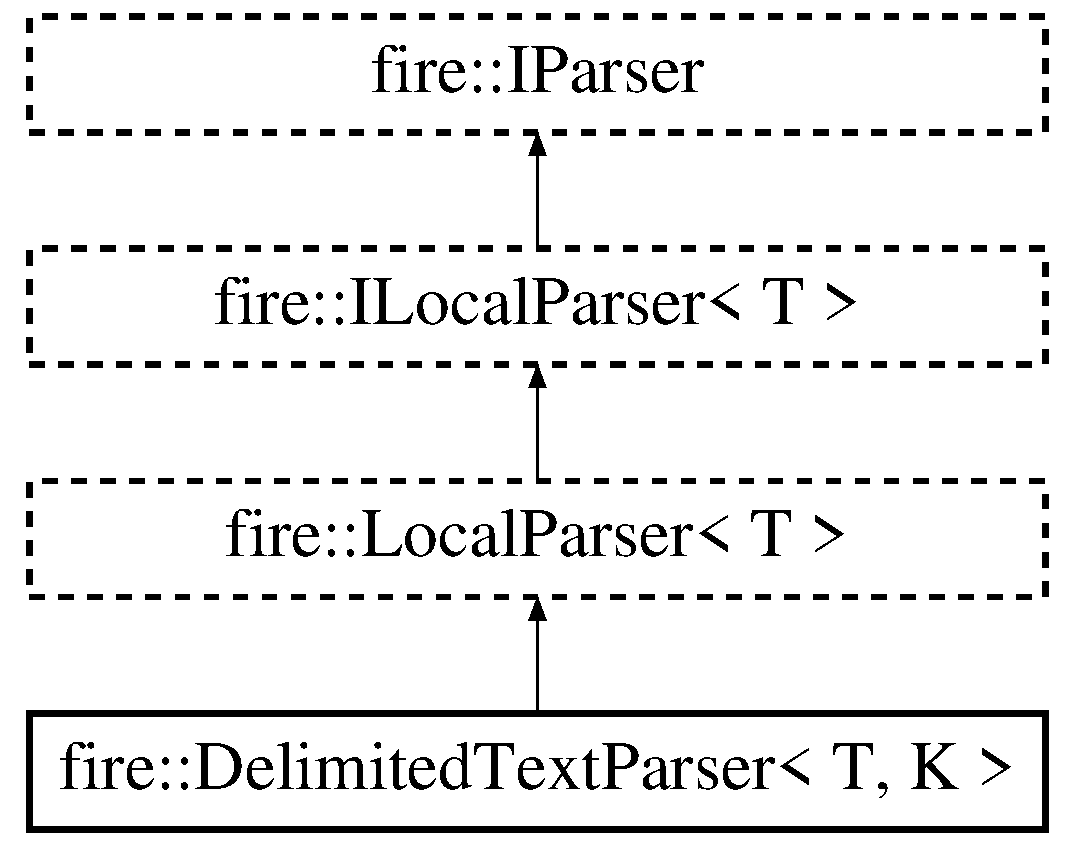
\includegraphics[height=4.000000cm]{a01736}
\end{center}
\end{figure}
\subsection*{Public Member Functions}
\begin{DoxyCompactItemize}
\item 
\mbox{\Hypertarget{a01736_aa1f041ebbf0bf72145e8bd20bf95f3f4}\label{a01736_aa1f041ebbf0bf72145e8bd20bf95f3f4}} 
{\bfseries Delimited\+Text\+Parser} (string delim, string comment)
\item 
virtual void \hyperlink{a01736_a686df5548771cae833d5e721442a821a}{parse} ()
\item 
{\footnotesize template$<$$>$ }\\void \hyperlink{a01736_a773fa7ed28cb9d8c384ad94bd81fc93f}{parse} ()
\end{DoxyCompactItemize}
\subsection*{Protected Attributes}
\begin{DoxyCompactItemize}
\item 
string \hyperlink{a01736_ac817fc333b53611a41f446977461bdbf}{delimiter}
\item 
string \hyperlink{a01736_acdd7b27b8109ed41e7d9bc5e6de72e93}{comment\+Char}
\end{DoxyCompactItemize}


\subsection{Detailed Description}
\subsubsection*{template$<$typename T, typename K$>$\newline
class fire\+::\+Delimited\+Text\+Parser$<$ T, K $>$}

This class implements \hyperlink{a01740}{I\+Local\+Parser} to provide a local, file-\/based, serially executed delimited text parser.

\hyperlink{a01740_a091d5cf56bf8f407854ef87f460b2958}{is\+File()} will return true if set\+Source(string) is used is\+Stream() will return true if set\+Source(istream) is used \hyperlink{a01740_a770acae6e216de3a9c7140a12de25d58}{is\+Local()} always returns true. \hyperlink{a01740_ad46898c516adcce38acbb4800dc9777b}{is\+Parallel()} always returns false.

Because delimited text is most often primitives, this class requires two template arguments. The first argument T is how the data should be returned and the second argument K is the root type of the delimited text, most likely a primitive. This would look something like


\begin{DoxyCode}
DelimitedTextParser<vector<vector<double>>,\textcolor{keywordtype}{double}>
\end{DoxyCode}


for a dense body of text like in a standard C\+SV file or D\+AT file where each column is composed of dense primitives.

The source may either be a file on the local filesystem or an input stream.

This is an extension of the parser interface that focuses on parsing delimited text. Delimited text is text with entries that are separated by a common pattern, such as a common or space.

The Comma-\/\+Separated Variables format is a delimited text format of the form

v1, v2, v3, v4

where each comma is the delimiter between the text values v1 through v4. A line of text with only spaces is also a delimited text format\+:

v1 v2 v3 v4

Delimited text parsers may assume that lines such as those above are terminated by ~\newline
. Like most other text formats, delimited text files may contain comments, which may be skipped by I\+Delimited\+Text\+Parsers. The characters that denote comments -\/ very commonly a \char`\"{}\#\char`\"{} or \char`\"{}//\char`\"{} -\/ may be passed to the constructor. 

\subsection{Member Function Documentation}
\mbox{\Hypertarget{a01736_a686df5548771cae833d5e721442a821a}\label{a01736_a686df5548771cae833d5e721442a821a}} 
\index{fire\+::\+Delimited\+Text\+Parser@{fire\+::\+Delimited\+Text\+Parser}!parse@{parse}}
\index{parse@{parse}!fire\+::\+Delimited\+Text\+Parser@{fire\+::\+Delimited\+Text\+Parser}}
\subsubsection{\texorpdfstring{parse()}{parse()}\hspace{0.1cm}{\footnotesize\ttfamily [1/2]}}
{\footnotesize\ttfamily template$<$typename T , typename K $>$ \\
virtual void \hyperlink{a01736}{fire\+::\+Delimited\+Text\+Parser}$<$ T, K $>$\+::parse (\begin{DoxyParamCaption}{ }\end{DoxyParamCaption})\hspace{0.3cm}{\ttfamily [inline]}, {\ttfamily [virtual]}}

This operation directs the parser to parse its source. 

Reimplemented from \hyperlink{a01756_abd8929aea06c2dda40256d2e58236650}{fire\+::\+Local\+Parser$<$ T $>$}.

\mbox{\Hypertarget{a01736_a773fa7ed28cb9d8c384ad94bd81fc93f}\label{a01736_a773fa7ed28cb9d8c384ad94bd81fc93f}} 
\index{fire\+::\+Delimited\+Text\+Parser@{fire\+::\+Delimited\+Text\+Parser}!parse@{parse}}
\index{parse@{parse}!fire\+::\+Delimited\+Text\+Parser@{fire\+::\+Delimited\+Text\+Parser}}
\subsubsection{\texorpdfstring{parse()}{parse()}\hspace{0.1cm}{\footnotesize\ttfamily [2/2]}}
{\footnotesize\ttfamily template$<$$>$ \\
void \hyperlink{a01736}{fire\+::\+Delimited\+Text\+Parser}$<$ vector$<$ vector$<$ double $>$ $>$, double $>$\+::parse (\begin{DoxyParamCaption}{ }\end{DoxyParamCaption})\hspace{0.3cm}{\ttfamily [virtual]}}

This specialization is for dense data of primitive type double. 

Reimplemented from \hyperlink{a01756_abd8929aea06c2dda40256d2e58236650}{fire\+::\+Local\+Parser$<$ T $>$}.



\subsection{Member Data Documentation}
\mbox{\Hypertarget{a01736_acdd7b27b8109ed41e7d9bc5e6de72e93}\label{a01736_acdd7b27b8109ed41e7d9bc5e6de72e93}} 
\index{fire\+::\+Delimited\+Text\+Parser@{fire\+::\+Delimited\+Text\+Parser}!comment\+Char@{comment\+Char}}
\index{comment\+Char@{comment\+Char}!fire\+::\+Delimited\+Text\+Parser@{fire\+::\+Delimited\+Text\+Parser}}
\subsubsection{\texorpdfstring{comment\+Char}{commentChar}}
{\footnotesize\ttfamily template$<$typename T , typename K $>$ \\
string \hyperlink{a01736}{fire\+::\+Delimited\+Text\+Parser}$<$ T, K $>$\+::comment\+Char\hspace{0.3cm}{\ttfamily [protected]}}

The character that represents a comment and should be skipped. \mbox{\Hypertarget{a01736_ac817fc333b53611a41f446977461bdbf}\label{a01736_ac817fc333b53611a41f446977461bdbf}} 
\index{fire\+::\+Delimited\+Text\+Parser@{fire\+::\+Delimited\+Text\+Parser}!delimiter@{delimiter}}
\index{delimiter@{delimiter}!fire\+::\+Delimited\+Text\+Parser@{fire\+::\+Delimited\+Text\+Parser}}
\subsubsection{\texorpdfstring{delimiter}{delimiter}}
{\footnotesize\ttfamily template$<$typename T , typename K $>$ \\
string \hyperlink{a01736}{fire\+::\+Delimited\+Text\+Parser}$<$ T, K $>$\+::delimiter\hspace{0.3cm}{\ttfamily [protected]}}

The delimiter used when parsing the file. 

The documentation for this class was generated from the following file\+:\begin{DoxyCompactItemize}
\item 
Delimited\+Text\+Parser.\+h\end{DoxyCompactItemize}

\hypertarget{a01360}{}\section{boost\+:\+:dll\+:\+:detail\+:\+:destructor$<$ Class $>$ Struct Template Reference}
\label{a01360}\index{boost\+::dll\+::detail\+::destructor$<$ Class $>$@{boost\+::dll\+::detail\+::destructor$<$ Class $>$}}
\subsection*{Public Types}
\begin{DoxyCompactItemize}
\item 
\mbox{\Hypertarget{a01360_a155dbf742e9c6499f52041d0b9f061be}\label{a01360_a155dbf742e9c6499f52041d0b9f061be}} 
typedef void($\ast$ {\bfseries type}) (Class $\ast$const)
\item 
\mbox{\Hypertarget{a01360_a6a72bebfcaef05b746a9b4cf93d66c50}\label{a01360_a6a72bebfcaef05b746a9b4cf93d66c50}} 
typedef type {\bfseries standard\+\_\+t}
\item 
\mbox{\Hypertarget{a01360_aff7ad402a5e8d7c8d1d086f73f3acf88}\label{a01360_aff7ad402a5e8d7c8d1d086f73f3acf88}} 
typedef type {\bfseries deleting\+\_\+t}
\end{DoxyCompactItemize}
\subsection*{Public Member Functions}
\begin{DoxyCompactItemize}
\item 
\mbox{\Hypertarget{a01360_a95d55018849080c7d4c771b564e9b04e}\label{a01360_a95d55018849080c7d4c771b564e9b04e}} 
void \hyperlink{a01360_a95d55018849080c7d4c771b564e9b04e}{call\+\_\+standard} (Class $\ast$const ptr)
\begin{DoxyCompactList}\small\item\em Call the standard contructor. \end{DoxyCompactList}\item 
\mbox{\Hypertarget{a01360_aabc107ff82b8a6f7e5aed5bd84080b1f}\label{a01360_aabc107ff82b8a6f7e5aed5bd84080b1f}} 
void \hyperlink{a01360_aabc107ff82b8a6f7e5aed5bd84080b1f}{call\+\_\+deleting} (Class $\ast$const ptr)
\begin{DoxyCompactList}\small\item\em Call the deleting destructor. \end{DoxyCompactList}\item 
\mbox{\Hypertarget{a01360_a2bb22835888e89f460dcba879c39f521}\label{a01360_a2bb22835888e89f460dcba879c39f521}} 
bool \hyperlink{a01360_a2bb22835888e89f460dcba879c39f521}{has\+\_\+deleting} () const
\begin{DoxyCompactList}\small\item\em True if a deleting destructor could be loaded. \end{DoxyCompactList}\item 
\mbox{\Hypertarget{a01360_aa7aeeca366db1520388239dc470c9509}\label{a01360_aa7aeeca366db1520388239dc470c9509}} 
bool \hyperlink{a01360_aa7aeeca366db1520388239dc470c9509}{has\+\_\+standard} () const
\begin{DoxyCompactList}\small\item\em True if a standard destructor could be loaded. \end{DoxyCompactList}\item 
\mbox{\Hypertarget{a01360_a11c37bcf56ad6f904376fbaf86acc2ce}\label{a01360_a11c37bcf56ad6f904376fbaf86acc2ce}} 
bool \hyperlink{a01360_a11c37bcf56ad6f904376fbaf86acc2ce}{is\+\_\+empty} () const
\begin{DoxyCompactList}\small\item\em False if neither the deleting nor the standard destructor is available. \end{DoxyCompactList}\item 
\mbox{\Hypertarget{a01360_a45248a911612597c871150e12ad3208b}\label{a01360_a45248a911612597c871150e12ad3208b}} 
\hyperlink{a01360_a45248a911612597c871150e12ad3208b}{destructor} (const \hyperlink{a01360}{destructor} \&)=default
\begin{DoxyCompactList}\small\item\em Copy destructor. \end{DoxyCompactList}\item 
\mbox{\Hypertarget{a01360_abc1f0cdcc708f43049b7d11727e24f24}\label{a01360_abc1f0cdcc708f43049b7d11727e24f24}} 
\hyperlink{a01360_abc1f0cdcc708f43049b7d11727e24f24}{destructor} (const standard\+\_\+t \&\hyperlink{a01360_a5c588780f2142ca3492ea78c62fe472c}{standard}, const deleting\+\_\+t \&\hyperlink{a01360_a96ad279626c7f9b845d47582f9f88dc0}{deleting}=nullptr)
\begin{DoxyCompactList}\small\item\em Construct it from both the standard destructor and the allocating destructor. \end{DoxyCompactList}\end{DoxyCompactItemize}
\subsection*{Public Attributes}
\begin{DoxyCompactItemize}
\item 
standard\+\_\+t \hyperlink{a01360_a5c588780f2142ca3492ea78c62fe472c}{standard}
\begin{DoxyCompactList}\small\item\em The standard, i.\+e. not deleting destructor. \end{DoxyCompactList}\item 
deleting\+\_\+t \hyperlink{a01360_a96ad279626c7f9b845d47582f9f88dc0}{deleting}
\begin{DoxyCompactList}\small\item\em The deleting destructor. \end{DoxyCompactList}\end{DoxyCompactItemize}


\subsection{Member Data Documentation}
\mbox{\Hypertarget{a01360_a96ad279626c7f9b845d47582f9f88dc0}\label{a01360_a96ad279626c7f9b845d47582f9f88dc0}} 
\index{boost\+::dll\+::detail\+::destructor@{boost\+::dll\+::detail\+::destructor}!deleting@{deleting}}
\index{deleting@{deleting}!boost\+::dll\+::detail\+::destructor@{boost\+::dll\+::detail\+::destructor}}
\subsubsection{\texorpdfstring{deleting}{deleting}}
{\footnotesize\ttfamily template$<$typename Class$>$ \\
deleting\+\_\+t \hyperlink{a01360}{boost\+::dll\+::detail\+::destructor}$<$ Class $>$\+::deleting}



The deleting destructor. 

\begin{DoxyWarning}{Warning}
May differ with the compiler. Use destructor\+::call\+\_\+deallocating instead. 
\end{DoxyWarning}
\mbox{\Hypertarget{a01360_a5c588780f2142ca3492ea78c62fe472c}\label{a01360_a5c588780f2142ca3492ea78c62fe472c}} 
\index{boost\+::dll\+::detail\+::destructor@{boost\+::dll\+::detail\+::destructor}!standard@{standard}}
\index{standard@{standard}!boost\+::dll\+::detail\+::destructor@{boost\+::dll\+::detail\+::destructor}}
\subsubsection{\texorpdfstring{standard}{standard}}
{\footnotesize\ttfamily template$<$typename Class$>$ \\
standard\+\_\+t \hyperlink{a01360}{boost\+::dll\+::detail\+::destructor}$<$ Class $>$\+::standard}



The standard, i.\+e. not deleting destructor. 

\begin{DoxyWarning}{Warning}
May differ with the compiler. Use \hyperlink{a01360_a95d55018849080c7d4c771b564e9b04e}{destructor\+::call\+\_\+standard} instead. 
\end{DoxyWarning}


The documentation for this struct was generated from the following file\+:\begin{DoxyCompactItemize}
\item 
ctor\+\_\+dtor.\+hpp\end{DoxyCompactItemize}

\hypertarget{a02252}{}\section{internal\+:\+:Diy\+Fp Struct Reference}
\label{a02252}\index{internal\+::\+Diy\+Fp@{internal\+::\+Diy\+Fp}}
\subsection*{Public Member Functions}
\begin{DoxyCompactItemize}
\item 
\mbox{\Hypertarget{a02252_a9a8f2f5c49dfa0dee4a527f0829cc2e5}\label{a02252_a9a8f2f5c49dfa0dee4a527f0829cc2e5}} 
{\bfseries Diy\+Fp} (uint64\+\_\+t fp, int exp)
\item 
\mbox{\Hypertarget{a02252_adc132c7da4c8e3ee5ae12efdcf6dbf7c}\label{a02252_adc132c7da4c8e3ee5ae12efdcf6dbf7c}} 
{\bfseries Diy\+Fp} (double d)
\item 
\mbox{\Hypertarget{a02252_a9cea201daabec04c6f2526b35af8ead3}\label{a02252_a9cea201daabec04c6f2526b35af8ead3}} 
\hyperlink{a02252}{Diy\+Fp} {\bfseries operator-\/} (const \hyperlink{a02252}{Diy\+Fp} \&rhs) const
\item 
\hyperlink{a02252}{Diy\+Fp} \hyperlink{a02252_a9868841f824924cc385ad5163c9c85b3}{operator$\ast$} (const \hyperlink{a02252}{Diy\+Fp} \&rhs) const
\item 
\mbox{\Hypertarget{a02252_aa6cbacc8dfcd92cb8c57884e45548976}\label{a02252_aa6cbacc8dfcd92cb8c57884e45548976}} 
\hyperlink{a02252}{Diy\+Fp} {\bfseries Normalize} () const
\item 
\mbox{\Hypertarget{a02252_a3a840e739b412e20e11c05a03f4573df}\label{a02252_a3a840e739b412e20e11c05a03f4573df}} 
\hyperlink{a02252}{Diy\+Fp} {\bfseries Normalize\+Boundary} () const
\item 
\mbox{\Hypertarget{a02252_adef8bf723f24db9dc6cefa260e8c2390}\label{a02252_adef8bf723f24db9dc6cefa260e8c2390}} 
void {\bfseries Normalized\+Boundaries} (\hyperlink{a02252}{Diy\+Fp} $\ast$minus, \hyperlink{a02252}{Diy\+Fp} $\ast$plus) const
\item 
\mbox{\Hypertarget{a02252_acf0e7974f0a1175ae04edf8e4a7d1319}\label{a02252_acf0e7974f0a1175ae04edf8e4a7d1319}} 
double {\bfseries To\+Double} () const
\end{DoxyCompactItemize}
\subsection*{Public Attributes}
\begin{DoxyCompactItemize}
\item 
\mbox{\Hypertarget{a02252_a09b9217a86e8a2e6aa8d2d48fc351008}\label{a02252_a09b9217a86e8a2e6aa8d2d48fc351008}} 
uint64\+\_\+t {\bfseries f}
\item 
\mbox{\Hypertarget{a02252_afa9db335eeb61c7f966d888d89b1e6f2}\label{a02252_afa9db335eeb61c7f966d888d89b1e6f2}} 
int {\bfseries e}
\end{DoxyCompactItemize}
\subsection*{Static Public Attributes}
\begin{DoxyCompactItemize}
\item 
\mbox{\Hypertarget{a02252_aac30e0c32d43425ac403281fc9b0cee4}\label{a02252_aac30e0c32d43425ac403281fc9b0cee4}} 
static const int {\bfseries k\+Diy\+Significand\+Size} = 64
\item 
\mbox{\Hypertarget{a02252_a037aed0fa0b66af0a13657418edef19e}\label{a02252_a037aed0fa0b66af0a13657418edef19e}} 
static const int {\bfseries k\+Dp\+Significand\+Size} = 52
\item 
\mbox{\Hypertarget{a02252_a38b6f864ae0859d43fa96c3ff27959be}\label{a02252_a38b6f864ae0859d43fa96c3ff27959be}} 
static const int {\bfseries k\+Dp\+Exponent\+Bias} = 0x3\+F\+F + k\+Dp\+Significand\+Size
\item 
\mbox{\Hypertarget{a02252_a80535a5594dae96fc482757a54162c7d}\label{a02252_a80535a5594dae96fc482757a54162c7d}} 
static const int {\bfseries k\+Dp\+Max\+Exponent} = 0x7\+F\+F -\/ k\+Dp\+Exponent\+Bias
\item 
\mbox{\Hypertarget{a02252_a9ad1b0cdbab318e45d2bc48e64707ef3}\label{a02252_a9ad1b0cdbab318e45d2bc48e64707ef3}} 
static const int {\bfseries k\+Dp\+Min\+Exponent} = -\/k\+Dp\+Exponent\+Bias
\item 
\mbox{\Hypertarget{a02252_a994f16a1247a290cfc3a875715e3a92b}\label{a02252_a994f16a1247a290cfc3a875715e3a92b}} 
static const int {\bfseries k\+Dp\+Denormal\+Exponent} = -\/k\+Dp\+Exponent\+Bias + 1
\item 
\mbox{\Hypertarget{a02252_aaacbf068c44275f4451db750938bd1d3}\label{a02252_aaacbf068c44275f4451db750938bd1d3}} 
static const uint64\+\_\+t {\bfseries k\+Dp\+Exponent\+Mask} = \hyperlink{a00560_aaee1245f375a71be1ac9b8a07ba5fb8f}{R\+A\+P\+I\+D\+J\+S\+O\+N\+\_\+\+U\+I\+N\+T64\+\_\+\+C2}(0x7\+F\+F00000, 0x00000000)
\item 
\mbox{\Hypertarget{a02252_a841ef0ae29ccd2889e7f96aad76b0179}\label{a02252_a841ef0ae29ccd2889e7f96aad76b0179}} 
static const uint64\+\_\+t {\bfseries k\+Dp\+Significand\+Mask} = \hyperlink{a00560_aaee1245f375a71be1ac9b8a07ba5fb8f}{R\+A\+P\+I\+D\+J\+S\+O\+N\+\_\+\+U\+I\+N\+T64\+\_\+\+C2}(0x000\+F\+F\+F\+F\+F, 0x\+F\+F\+F\+F\+F\+F\+F\+F)
\item 
\mbox{\Hypertarget{a02252_a43ea451ce20095b1ff53cccf132ca15f}\label{a02252_a43ea451ce20095b1ff53cccf132ca15f}} 
static const uint64\+\_\+t {\bfseries k\+Dp\+Hidden\+Bit} = \hyperlink{a00560_aaee1245f375a71be1ac9b8a07ba5fb8f}{R\+A\+P\+I\+D\+J\+S\+O\+N\+\_\+\+U\+I\+N\+T64\+\_\+\+C2}(0x00100000, 0x00000000)
\end{DoxyCompactItemize}


\subsection{Member Function Documentation}
\mbox{\Hypertarget{a02252_a9868841f824924cc385ad5163c9c85b3}\label{a02252_a9868841f824924cc385ad5163c9c85b3}} 
\index{internal\+::\+Diy\+Fp@{internal\+::\+Diy\+Fp}!operator$\ast$@{operator$\ast$}}
\index{operator$\ast$@{operator$\ast$}!internal\+::\+Diy\+Fp@{internal\+::\+Diy\+Fp}}
\subsubsection{\texorpdfstring{operator$\ast$()}{operator*()}}
{\footnotesize\ttfamily \hyperlink{a02252}{Diy\+Fp} internal\+::\+Diy\+Fp\+::operator$\ast$ (\begin{DoxyParamCaption}\item[{const \hyperlink{a02252}{Diy\+Fp} \&}]{rhs }\end{DoxyParamCaption}) const\hspace{0.3cm}{\ttfamily [inline]}}

mult\+\_\+round 

The documentation for this struct was generated from the following file\+:\begin{DoxyCompactItemize}
\item 
diyfp.\+h\end{DoxyCompactItemize}

\hypertarget{a02256}{}\section{internal\+:\+:Double Class Reference}
\label{a02256}\index{internal\+::\+Double@{internal\+::\+Double}}
\subsection*{Public Member Functions}
\begin{DoxyCompactItemize}
\item 
\mbox{\Hypertarget{a02256_ad66f3b914570ce62e9f16083117f3e4f}\label{a02256_ad66f3b914570ce62e9f16083117f3e4f}} 
{\bfseries Double} (double d)
\item 
\mbox{\Hypertarget{a02256_a293a7ca841d847ea3e83ffa28b68601f}\label{a02256_a293a7ca841d847ea3e83ffa28b68601f}} 
{\bfseries Double} (uint64\+\_\+t u)
\item 
\mbox{\Hypertarget{a02256_a665c64824d1046528cbc4066a9ed0ef8}\label{a02256_a665c64824d1046528cbc4066a9ed0ef8}} 
double {\bfseries Value} () const
\item 
\mbox{\Hypertarget{a02256_a1a35be6344c886f159cb36a1498a62ac}\label{a02256_a1a35be6344c886f159cb36a1498a62ac}} 
uint64\+\_\+t {\bfseries Uint64\+Value} () const
\item 
\mbox{\Hypertarget{a02256_a6ffee23d82d9c606b1a53ed87e393e90}\label{a02256_a6ffee23d82d9c606b1a53ed87e393e90}} 
double {\bfseries Next\+Positive\+Double} () const
\item 
\mbox{\Hypertarget{a02256_ab09c26873ca4c3e471a97c4559bf317d}\label{a02256_ab09c26873ca4c3e471a97c4559bf317d}} 
bool {\bfseries Sign} () const
\item 
\mbox{\Hypertarget{a02256_ade5d3e893dd6884ccd37632109dae1a6}\label{a02256_ade5d3e893dd6884ccd37632109dae1a6}} 
uint64\+\_\+t {\bfseries Significand} () const
\item 
\mbox{\Hypertarget{a02256_ae091055d96d8730f654170613f2cf265}\label{a02256_ae091055d96d8730f654170613f2cf265}} 
int {\bfseries Exponent} () const
\item 
\mbox{\Hypertarget{a02256_a312312ab2798ee85cbd0e739fcefa386}\label{a02256_a312312ab2798ee85cbd0e739fcefa386}} 
bool {\bfseries Is\+Nan} () const
\item 
\mbox{\Hypertarget{a02256_afe1ce48f7fb9797e1a2044c58a6b226c}\label{a02256_afe1ce48f7fb9797e1a2044c58a6b226c}} 
bool {\bfseries Is\+Inf} () const
\item 
\mbox{\Hypertarget{a02256_a8b9a82e8b99783b7e98b5307756021c0}\label{a02256_a8b9a82e8b99783b7e98b5307756021c0}} 
bool {\bfseries Is\+Nan\+Or\+Inf} () const
\item 
\mbox{\Hypertarget{a02256_a8a39cd42010c69681da35d87f1331381}\label{a02256_a8a39cd42010c69681da35d87f1331381}} 
bool {\bfseries Is\+Normal} () const
\item 
\mbox{\Hypertarget{a02256_a90a3a1ca614b377b59576955ce987ce2}\label{a02256_a90a3a1ca614b377b59576955ce987ce2}} 
bool {\bfseries Is\+Zero} () const
\item 
\mbox{\Hypertarget{a02256_a1bf89d77be843f69facec9f2bc4dbc72}\label{a02256_a1bf89d77be843f69facec9f2bc4dbc72}} 
uint64\+\_\+t {\bfseries Integer\+Significand} () const
\item 
\mbox{\Hypertarget{a02256_a9721e0fdedef4d0fe6c7b411492a88fb}\label{a02256_a9721e0fdedef4d0fe6c7b411492a88fb}} 
int {\bfseries Integer\+Exponent} () const
\item 
\mbox{\Hypertarget{a02256_ab3d3a81274e4f4b9b415db7c664d3ac9}\label{a02256_ab3d3a81274e4f4b9b415db7c664d3ac9}} 
uint64\+\_\+t {\bfseries To\+Bias} () const
\end{DoxyCompactItemize}
\subsection*{Static Public Member Functions}
\begin{DoxyCompactItemize}
\item 
\mbox{\Hypertarget{a02256_aa710fa4f5e06b0ff4348a13475688f13}\label{a02256_aa710fa4f5e06b0ff4348a13475688f13}} 
static int {\bfseries Effective\+Significand\+Size} (int order)
\end{DoxyCompactItemize}


The documentation for this class was generated from the following file\+:\begin{DoxyCompactItemize}
\item 
ieee754.\+h\end{DoxyCompactItemize}

\hypertarget{a01376}{}\section{boost\+:\+:dll\+:\+:detail\+:\+:mangled\+\_\+storage\+\_\+impl\+:\+:dtor\+\_\+sym Struct Reference}
\label{a01376}\index{boost\+::dll\+::detail\+::mangled\+\_\+storage\+\_\+impl\+::dtor\+\_\+sym@{boost\+::dll\+::detail\+::mangled\+\_\+storage\+\_\+impl\+::dtor\+\_\+sym}}
\subsection*{Public Member Functions}
\begin{DoxyCompactItemize}
\item 
\mbox{\Hypertarget{a01376_ab144596e9b758af754d0ccb1b968c67f}\label{a01376_ab144596e9b758af754d0ccb1b968c67f}} 
bool {\bfseries empty} () const
\end{DoxyCompactItemize}
\subsection*{Public Attributes}
\begin{DoxyCompactItemize}
\item 
\mbox{\Hypertarget{a01376_a17ef5095bb94db1ef8a318012710939a}\label{a01376_a17ef5095bb94db1ef8a318012710939a}} 
std\+::string {\bfseries D0}
\item 
\mbox{\Hypertarget{a01376_af5d75b054b254565c9773f8b0b652d4b}\label{a01376_af5d75b054b254565c9773f8b0b652d4b}} 
std\+::string {\bfseries D1}
\item 
\mbox{\Hypertarget{a01376_ae40fab2db5138e03488b204b570ac72d}\label{a01376_ae40fab2db5138e03488b204b570ac72d}} 
std\+::string {\bfseries D2}
\end{DoxyCompactItemize}


The documentation for this struct was generated from the following file\+:\begin{DoxyCompactItemize}
\item 
itanium.\+hpp\end{DoxyCompactItemize}

\hypertarget{a02500}{}\section{Dummy\+Compiler Class Reference}
\label{a02500}\index{Dummy\+Compiler@{Dummy\+Compiler}}
Inheritance diagram for Dummy\+Compiler\+:\begin{figure}[H]
\begin{center}
\leavevmode
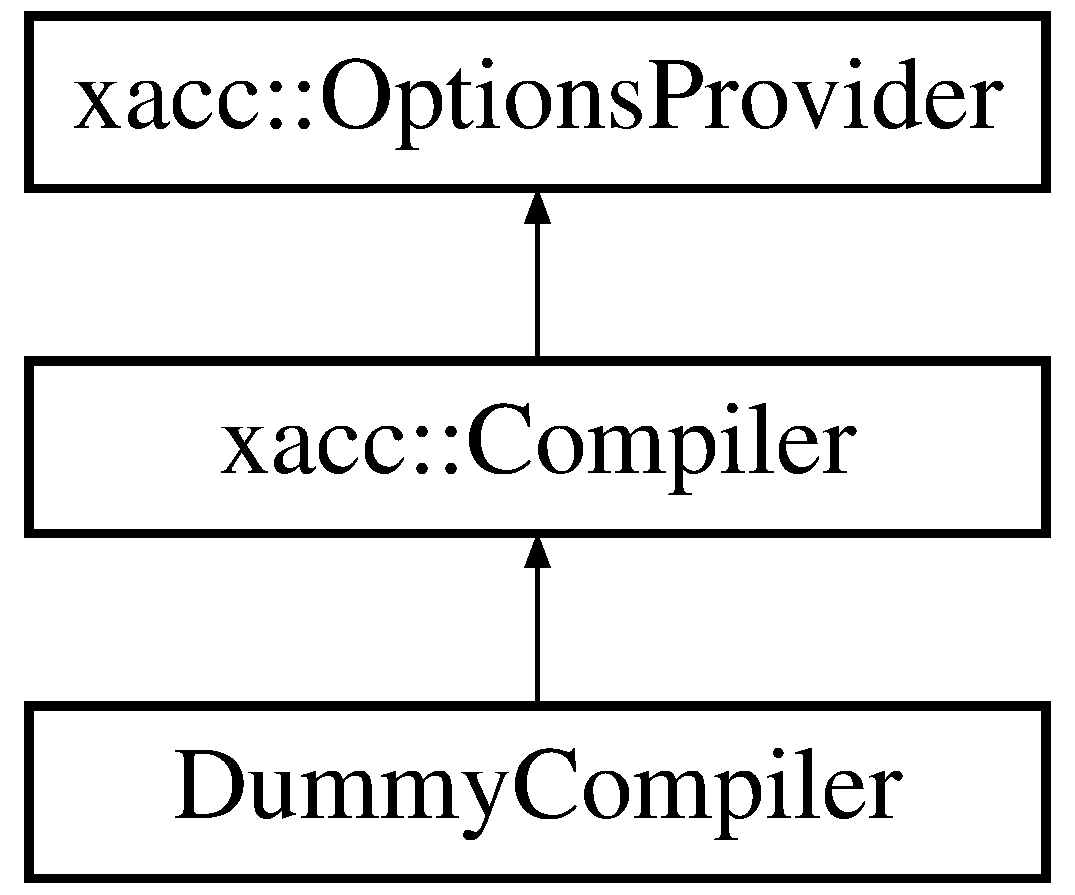
\includegraphics[height=3.000000cm]{a02500}
\end{center}
\end{figure}
\subsection*{Public Member Functions}
\begin{DoxyCompactItemize}
\item 
virtual std\+::shared\+\_\+ptr$<$ \hyperlink{a02480}{xacc\+::\+IR} $>$ \hyperlink{a02500_acc75af818d62ba22d1dd7de3b66c4baf}{compile} (const std\+::string \&src, std\+::shared\+\_\+ptr$<$ \hyperlink{a02432}{Accelerator} $>$ acc)
\item 
virtual std\+::shared\+\_\+ptr$<$ \hyperlink{a02480}{xacc\+::\+IR} $>$ \hyperlink{a02500_a40d7cc3bbc72a2ce9362136b3b83245c}{compile} (const std\+::string \&src)
\item 
virtual const std\+::string \hyperlink{a02500_a76460cb78671dc2cf42f2bebf8fb80c7}{get\+Name} ()
\item 
\mbox{\Hypertarget{a02500_a9f58a296f96aa340fc73b267f8c80fb0}\label{a02500_a9f58a296f96aa340fc73b267f8c80fb0}} 
virtual void {\bfseries modify\+Source} ()
\item 
\mbox{\Hypertarget{a02500_a1a9739b20fb26d1f440bdd6cdfab0d8a}\label{a02500_a1a9739b20fb26d1f440bdd6cdfab0d8a}} 
virtual std\+::string {\bfseries get\+Bit\+Type} ()
\end{DoxyCompactItemize}
\subsection*{Additional Inherited Members}


\subsection{Member Function Documentation}
\mbox{\Hypertarget{a02500_acc75af818d62ba22d1dd7de3b66c4baf}\label{a02500_acc75af818d62ba22d1dd7de3b66c4baf}} 
\index{Dummy\+Compiler@{Dummy\+Compiler}!compile@{compile}}
\index{compile@{compile}!Dummy\+Compiler@{Dummy\+Compiler}}
\subsubsection{\texorpdfstring{compile()}{compile()}\hspace{0.1cm}{\footnotesize\ttfamily [1/2]}}
{\footnotesize\ttfamily virtual std\+::shared\+\_\+ptr$<$\hyperlink{a02480}{xacc\+::\+IR}$>$ Dummy\+Compiler\+::compile (\begin{DoxyParamCaption}\item[{const std\+::string \&}]{src,  }\item[{std\+::shared\+\_\+ptr$<$ \hyperlink{a02432}{Accelerator} $>$}]{acc }\end{DoxyParamCaption})\hspace{0.3cm}{\ttfamily [inline]}, {\ttfamily [virtual]}}

This method is to be implemented by derived Compilers and is in charge of executing the compilation mechanism on the provided source string. Implementations also are given access to the Accelerator that this source code is intended for.


\begin{DoxyParams}{Parameters}
{\em src} & The kernel source string. \\
\hline
{\em acc} & The Accelerator this code will be executed on \\
\hline
\end{DoxyParams}
\begin{DoxyReturn}{Returns}
ir Intermediate representation for provided source kernel code. 
\end{DoxyReturn}


Implements \hyperlink{a02448_a546a40c95bb93af6a0c0ac48dbeaffc8}{xacc\+::\+Compiler}.

\mbox{\Hypertarget{a02500_a40d7cc3bbc72a2ce9362136b3b83245c}\label{a02500_a40d7cc3bbc72a2ce9362136b3b83245c}} 
\index{Dummy\+Compiler@{Dummy\+Compiler}!compile@{compile}}
\index{compile@{compile}!Dummy\+Compiler@{Dummy\+Compiler}}
\subsubsection{\texorpdfstring{compile()}{compile()}\hspace{0.1cm}{\footnotesize\ttfamily [2/2]}}
{\footnotesize\ttfamily virtual std\+::shared\+\_\+ptr$<$\hyperlink{a02480}{xacc\+::\+IR}$>$ Dummy\+Compiler\+::compile (\begin{DoxyParamCaption}\item[{const std\+::string \&}]{src }\end{DoxyParamCaption})\hspace{0.3cm}{\ttfamily [inline]}, {\ttfamily [virtual]}}

This method is to be implemented by derived Compilers and is in charge of executing the compilation mechanism on the provided source string. 
\begin{DoxyParams}{Parameters}
{\em src} & \\
\hline
\end{DoxyParams}
\begin{DoxyReturn}{Returns}

\end{DoxyReturn}


Implements \hyperlink{a02448_a9092f5f779b570c91569b59621280c04}{xacc\+::\+Compiler}.

\mbox{\Hypertarget{a02500_a76460cb78671dc2cf42f2bebf8fb80c7}\label{a02500_a76460cb78671dc2cf42f2bebf8fb80c7}} 
\index{Dummy\+Compiler@{Dummy\+Compiler}!get\+Name@{get\+Name}}
\index{get\+Name@{get\+Name}!Dummy\+Compiler@{Dummy\+Compiler}}
\subsubsection{\texorpdfstring{get\+Name()}{getName()}}
{\footnotesize\ttfamily virtual const std\+::string Dummy\+Compiler\+::get\+Name (\begin{DoxyParamCaption}{ }\end{DoxyParamCaption})\hspace{0.3cm}{\ttfamily [inline]}, {\ttfamily [virtual]}}

Return the name of this Compiler \begin{DoxyReturn}{Returns}
name Compiler name 
\end{DoxyReturn}


Implements \hyperlink{a02448_a87fca9100e6462122f5b687c3a0fb3fb}{xacc\+::\+Compiler}.



The documentation for this class was generated from the following file\+:\begin{DoxyCompactItemize}
\item 
Program\+Tester.\+cpp\end{DoxyCompactItemize}

\hypertarget{a01332}{}\section{Dummy\+Gate Class Reference}
\label{a01332}\index{Dummy\+Gate@{Dummy\+Gate}}
Inheritance diagram for Dummy\+Gate\+:\begin{figure}[H]
\begin{center}
\leavevmode
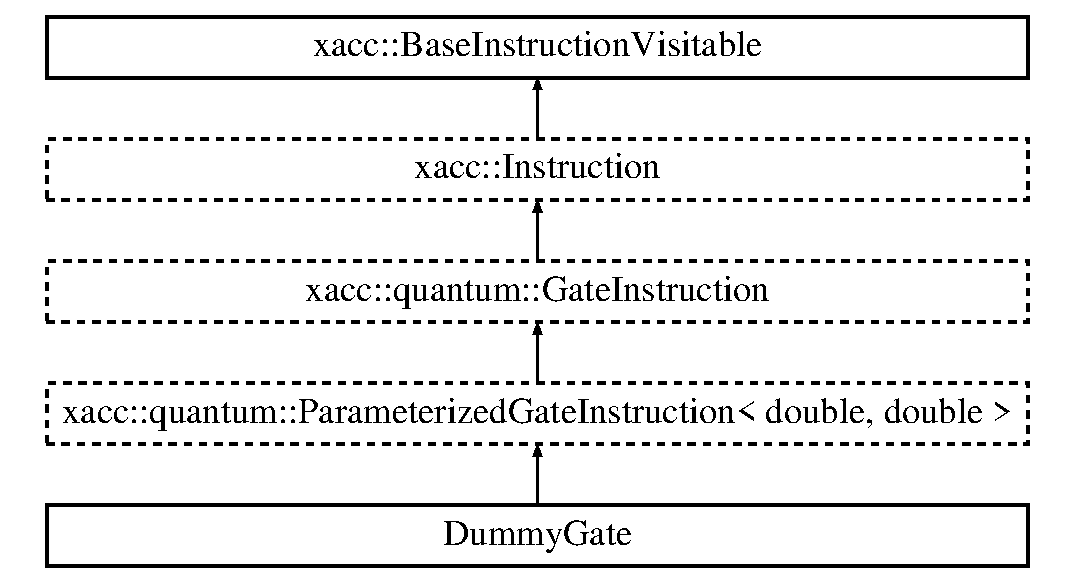
\includegraphics[height=5.000000cm]{a01332}
\end{center}
\end{figure}
\subsection*{Public Member Functions}
\begin{DoxyCompactItemize}
\item 
\mbox{\Hypertarget{a01332_a64005aff4bba279a321a3d24695834eb}\label{a01332_a64005aff4bba279a321a3d24695834eb}} 
{\bfseries Dummy\+Gate} (int qbit, double param1, double param2)
\end{DoxyCompactItemize}
\subsection*{Additional Inherited Members}


The documentation for this class was generated from the following file\+:\begin{DoxyCompactItemize}
\item 
Parameterized\+Gate\+Tester.\+cpp\end{DoxyCompactItemize}

\hypertarget{a01252}{}\section{xacc\+:\+:quantum\+:\+:D\+Wave\+Compiler Class Reference}
\label{a01252}\index{xacc\+::quantum\+::\+D\+Wave\+Compiler@{xacc\+::quantum\+::\+D\+Wave\+Compiler}}
Inheritance diagram for xacc\+:\+:quantum\+:\+:D\+Wave\+Compiler\+:\begin{figure}[H]
\begin{center}
\leavevmode
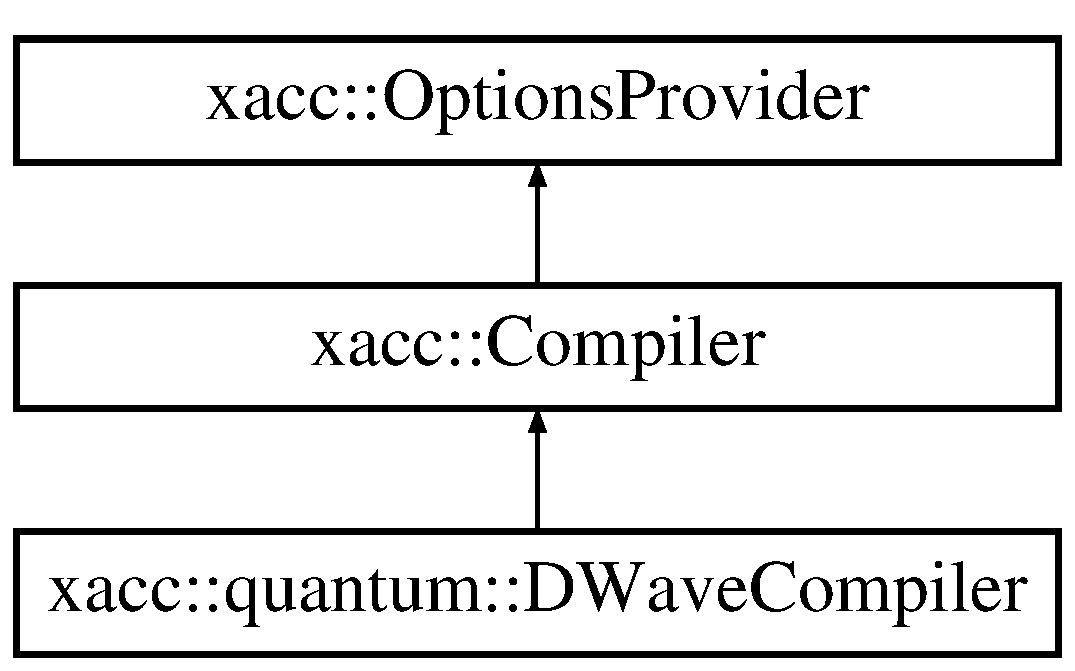
\includegraphics[height=3.000000cm]{a01252}
\end{center}
\end{figure}
\subsection*{Public Member Functions}
\begin{DoxyCompactItemize}
\item 
virtual std\+::shared\+\_\+ptr$<$ \hyperlink{a02480}{xacc\+::\+IR} $>$ \hyperlink{a01252_a0f7f6b10b4a881cb27b36eaa6d39e7b1}{compile} (const std\+::string \&src, std\+::shared\+\_\+ptr$<$ \hyperlink{a02432}{Accelerator} $>$ acc)
\item 
virtual std\+::shared\+\_\+ptr$<$ \hyperlink{a02480}{xacc\+::\+IR} $>$ \hyperlink{a01252_a893e1d1c81a8aaf6e2435c9bceab575e}{compile} (const std\+::string \&src)
\item 
virtual const std\+::string \hyperlink{a01252_a8a180031ae563e1a9aac611e8066c181}{get\+Name} ()
\item 
virtual \hyperlink{a01252_acc0ab28f787b8f4cbeb63c594a247e50}{$\sim$\+D\+Wave\+Compiler} ()
\end{DoxyCompactItemize}
\subsection*{Static Public Member Functions}
\begin{DoxyCompactItemize}
\item 
static void \hyperlink{a01252_a5b221649f22a9bb4d4a304a6522d071f}{register\+Compiler} ()
\end{DoxyCompactItemize}
\subsection*{Additional Inherited Members}


\subsection{Constructor \& Destructor Documentation}
\mbox{\Hypertarget{a01252_acc0ab28f787b8f4cbeb63c594a247e50}\label{a01252_acc0ab28f787b8f4cbeb63c594a247e50}} 
\index{xacc\+::quantum\+::\+D\+Wave\+Compiler@{xacc\+::quantum\+::\+D\+Wave\+Compiler}!````~D\+Wave\+Compiler@{$\sim$\+D\+Wave\+Compiler}}
\index{````~D\+Wave\+Compiler@{$\sim$\+D\+Wave\+Compiler}!xacc\+::quantum\+::\+D\+Wave\+Compiler@{xacc\+::quantum\+::\+D\+Wave\+Compiler}}
\subsubsection{\texorpdfstring{$\sim$\+D\+Wave\+Compiler()}{~DWaveCompiler()}}
{\footnotesize\ttfamily virtual xacc\+::quantum\+::\+D\+Wave\+Compiler\+::$\sim$\+D\+Wave\+Compiler (\begin{DoxyParamCaption}{ }\end{DoxyParamCaption})\hspace{0.3cm}{\ttfamily [inline]}, {\ttfamily [virtual]}}

The destructor 

\subsection{Member Function Documentation}
\mbox{\Hypertarget{a01252_a0f7f6b10b4a881cb27b36eaa6d39e7b1}\label{a01252_a0f7f6b10b4a881cb27b36eaa6d39e7b1}} 
\index{xacc\+::quantum\+::\+D\+Wave\+Compiler@{xacc\+::quantum\+::\+D\+Wave\+Compiler}!compile@{compile}}
\index{compile@{compile}!xacc\+::quantum\+::\+D\+Wave\+Compiler@{xacc\+::quantum\+::\+D\+Wave\+Compiler}}
\subsubsection{\texorpdfstring{compile()}{compile()}\hspace{0.1cm}{\footnotesize\ttfamily [1/2]}}
{\footnotesize\ttfamily std\+::shared\+\_\+ptr$<$ \hyperlink{a02480}{IR} $>$ xacc\+::quantum\+::\+D\+Wave\+Compiler\+::compile (\begin{DoxyParamCaption}\item[{const std\+::string \&}]{src,  }\item[{std\+::shared\+\_\+ptr$<$ \hyperlink{a02432}{Accelerator} $>$}]{acc }\end{DoxyParamCaption})\hspace{0.3cm}{\ttfamily [virtual]}}

This method is to be implemented by derived Compilers and is in charge of executing the compilation mechanism on the provided source string. Implementations also are given access to the \hyperlink{a02432}{Accelerator} that this source code is intended for.


\begin{DoxyParams}{Parameters}
{\em src} & The kernel source string. \\
\hline
{\em acc} & The \hyperlink{a02432}{Accelerator} this code will be executed on \\
\hline
\end{DoxyParams}
\begin{DoxyReturn}{Returns}
ir Intermediate representation for provided source kernel code. 
\end{DoxyReturn}


Implements \hyperlink{a02448_a546a40c95bb93af6a0c0ac48dbeaffc8}{xacc\+::\+Compiler}.

\mbox{\Hypertarget{a01252_a893e1d1c81a8aaf6e2435c9bceab575e}\label{a01252_a893e1d1c81a8aaf6e2435c9bceab575e}} 
\index{xacc\+::quantum\+::\+D\+Wave\+Compiler@{xacc\+::quantum\+::\+D\+Wave\+Compiler}!compile@{compile}}
\index{compile@{compile}!xacc\+::quantum\+::\+D\+Wave\+Compiler@{xacc\+::quantum\+::\+D\+Wave\+Compiler}}
\subsubsection{\texorpdfstring{compile()}{compile()}\hspace{0.1cm}{\footnotesize\ttfamily [2/2]}}
{\footnotesize\ttfamily std\+::shared\+\_\+ptr$<$ \hyperlink{a02480}{IR} $>$ xacc\+::quantum\+::\+D\+Wave\+Compiler\+::compile (\begin{DoxyParamCaption}\item[{const std\+::string \&}]{src }\end{DoxyParamCaption})\hspace{0.3cm}{\ttfamily [virtual]}}

\begin{DoxyReturn}{Returns}

\end{DoxyReturn}


Implements \hyperlink{a02448_a9092f5f779b570c91569b59621280c04}{xacc\+::\+Compiler}.

\mbox{\Hypertarget{a01252_a8a180031ae563e1a9aac611e8066c181}\label{a01252_a8a180031ae563e1a9aac611e8066c181}} 
\index{xacc\+::quantum\+::\+D\+Wave\+Compiler@{xacc\+::quantum\+::\+D\+Wave\+Compiler}!get\+Name@{get\+Name}}
\index{get\+Name@{get\+Name}!xacc\+::quantum\+::\+D\+Wave\+Compiler@{xacc\+::quantum\+::\+D\+Wave\+Compiler}}
\subsubsection{\texorpdfstring{get\+Name()}{getName()}}
{\footnotesize\ttfamily virtual const std\+::string xacc\+::quantum\+::\+D\+Wave\+Compiler\+::get\+Name (\begin{DoxyParamCaption}{ }\end{DoxyParamCaption})\hspace{0.3cm}{\ttfamily [inline]}, {\ttfamily [virtual]}}

Return the name of this \hyperlink{a02448}{Compiler} \begin{DoxyReturn}{Returns}
name \hyperlink{a02448}{Compiler} name 
\end{DoxyReturn}


Implements \hyperlink{a02448_a87fca9100e6462122f5b687c3a0fb3fb}{xacc\+::\+Compiler}.

\mbox{\Hypertarget{a01252_a5b221649f22a9bb4d4a304a6522d071f}\label{a01252_a5b221649f22a9bb4d4a304a6522d071f}} 
\index{xacc\+::quantum\+::\+D\+Wave\+Compiler@{xacc\+::quantum\+::\+D\+Wave\+Compiler}!register\+Compiler@{register\+Compiler}}
\index{register\+Compiler@{register\+Compiler}!xacc\+::quantum\+::\+D\+Wave\+Compiler@{xacc\+::quantum\+::\+D\+Wave\+Compiler}}
\subsubsection{\texorpdfstring{register\+Compiler()}{registerCompiler()}}
{\footnotesize\ttfamily static void xacc\+::quantum\+::\+D\+Wave\+Compiler\+::register\+Compiler (\begin{DoxyParamCaption}{ }\end{DoxyParamCaption})\hspace{0.3cm}{\ttfamily [inline]}, {\ttfamily [static]}}

Register this \hyperlink{a02448}{Compiler} with the framework. 

The documentation for this class was generated from the following files\+:\begin{DoxyCompactItemize}
\item 
D\+Wave\+Compiler.\+hpp\item 
D\+Wave\+Compiler.\+cpp\end{DoxyCompactItemize}

\hypertarget{a01268}{}\section{xacc\+:\+:quantum\+:\+:D\+Wave\+IR Class Reference}
\label{a01268}\index{xacc\+::quantum\+::\+D\+Wave\+IR@{xacc\+::quantum\+::\+D\+Wave\+IR}}
Inheritance diagram for xacc\+:\+:quantum\+:\+:D\+Wave\+IR\+:\begin{figure}[H]
\begin{center}
\leavevmode
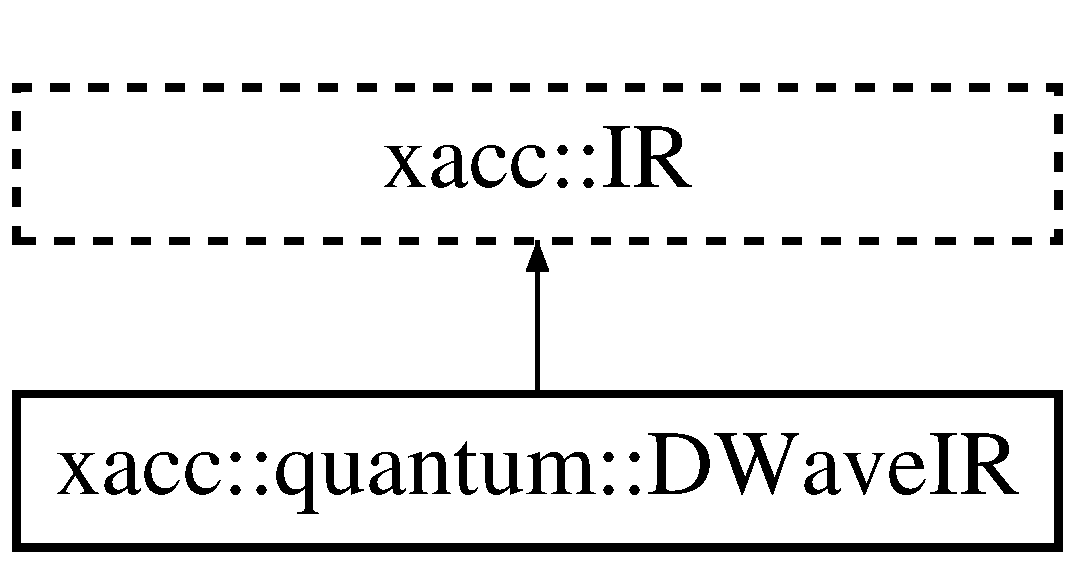
\includegraphics[height=2.000000cm]{a01268}
\end{center}
\end{figure}
\subsection*{Public Member Functions}
\begin{DoxyCompactItemize}
\item 
virtual std\+::string \hyperlink{a01268_ac19ad098d5bbfe769809c10e26ebebc6}{to\+Assembly\+String} (const std\+::string \&kernel\+Name, const std\+::string \&acc\+Buffer\+Var\+Name)
\item 
virtual void \hyperlink{a01268_adac268c6fa2234902efeb9b3c07c0ac2}{persist} (std\+::ostream \&out\+Stream)
\item 
virtual void \hyperlink{a01268_a94d814172ec30c7ed32e6ab52bc2a41a}{load} (std\+::istream \&in\+Stream)
\item 
virtual void \hyperlink{a01268_a7e1ddff2771233dc45f60a6b7e15ef63}{add\+Kernel} (std\+::shared\+\_\+ptr$<$ \hyperlink{a02456}{Function} $>$ kernel)
\item 
virtual std\+::shared\+\_\+ptr$<$ \hyperlink{a02456}{Function} $>$ \hyperlink{a01268_ac4295dfef98c94d7154a4fd39a6e5d1c}{get\+Kernel} (const std\+::string \&name)
\end{DoxyCompactItemize}


\subsection{Member Function Documentation}
\mbox{\Hypertarget{a01268_a7e1ddff2771233dc45f60a6b7e15ef63}\label{a01268_a7e1ddff2771233dc45f60a6b7e15ef63}} 
\index{xacc\+::quantum\+::\+D\+Wave\+IR@{xacc\+::quantum\+::\+D\+Wave\+IR}!add\+Kernel@{add\+Kernel}}
\index{add\+Kernel@{add\+Kernel}!xacc\+::quantum\+::\+D\+Wave\+IR@{xacc\+::quantum\+::\+D\+Wave\+IR}}
\subsubsection{\texorpdfstring{add\+Kernel()}{addKernel()}}
{\footnotesize\ttfamily virtual void xacc\+::quantum\+::\+D\+Wave\+I\+R\+::add\+Kernel (\begin{DoxyParamCaption}\item[{std\+::shared\+\_\+ptr$<$ \hyperlink{a02456}{Function} $>$}]{kernel }\end{DoxyParamCaption})\hspace{0.3cm}{\ttfamily [inline]}, {\ttfamily [virtual]}}

Add a new kernel to this \hyperlink{a02480}{IR} instance.


\begin{DoxyParams}{Parameters}
{\em kernel} & The \hyperlink{a02456}{Function} instance to add as a new kernel \\
\hline
\end{DoxyParams}


Implements \hyperlink{a02480_abbbf8e6993c518597de32cd05d49d737}{xacc\+::\+IR}.

\mbox{\Hypertarget{a01268_ac4295dfef98c94d7154a4fd39a6e5d1c}\label{a01268_ac4295dfef98c94d7154a4fd39a6e5d1c}} 
\index{xacc\+::quantum\+::\+D\+Wave\+IR@{xacc\+::quantum\+::\+D\+Wave\+IR}!get\+Kernel@{get\+Kernel}}
\index{get\+Kernel@{get\+Kernel}!xacc\+::quantum\+::\+D\+Wave\+IR@{xacc\+::quantum\+::\+D\+Wave\+IR}}
\subsubsection{\texorpdfstring{get\+Kernel()}{getKernel()}}
{\footnotesize\ttfamily virtual std\+::shared\+\_\+ptr$<$\hyperlink{a02456}{Function}$>$ xacc\+::quantum\+::\+D\+Wave\+I\+R\+::get\+Kernel (\begin{DoxyParamCaption}\item[{const std\+::string \&}]{name }\end{DoxyParamCaption})\hspace{0.3cm}{\ttfamily [inline]}, {\ttfamily [virtual]}}

Return the kernel with the given name.


\begin{DoxyParams}{Parameters}
{\em name} & The name of the kernel to return. \\
\hline
\end{DoxyParams}
\begin{DoxyReturn}{Returns}
kernel The kernel with given name. 
\end{DoxyReturn}


Implements \hyperlink{a02480_a6f49b4ba4b3a15142b04873284885f0d}{xacc\+::\+IR}.

\mbox{\Hypertarget{a01268_a94d814172ec30c7ed32e6ab52bc2a41a}\label{a01268_a94d814172ec30c7ed32e6ab52bc2a41a}} 
\index{xacc\+::quantum\+::\+D\+Wave\+IR@{xacc\+::quantum\+::\+D\+Wave\+IR}!load@{load}}
\index{load@{load}!xacc\+::quantum\+::\+D\+Wave\+IR@{xacc\+::quantum\+::\+D\+Wave\+IR}}
\subsubsection{\texorpdfstring{load()}{load()}}
{\footnotesize\ttfamily virtual void xacc\+::quantum\+::\+D\+Wave\+I\+R\+::load (\begin{DoxyParamCaption}\item[{std\+::istream \&}]{in\+Stream }\end{DoxyParamCaption})\hspace{0.3cm}{\ttfamily [inline]}, {\ttfamily [virtual]}}

Create this \hyperlink{a02480}{IR} instance from the given input stream.


\begin{DoxyParams}{Parameters}
{\em in\+Stream} & \\
\hline
\end{DoxyParams}


Implements \hyperlink{a02480_a444c2e4dc0faac500fb70fa93997e9bc}{xacc\+::\+IR}.

\mbox{\Hypertarget{a01268_adac268c6fa2234902efeb9b3c07c0ac2}\label{a01268_adac268c6fa2234902efeb9b3c07c0ac2}} 
\index{xacc\+::quantum\+::\+D\+Wave\+IR@{xacc\+::quantum\+::\+D\+Wave\+IR}!persist@{persist}}
\index{persist@{persist}!xacc\+::quantum\+::\+D\+Wave\+IR@{xacc\+::quantum\+::\+D\+Wave\+IR}}
\subsubsection{\texorpdfstring{persist()}{persist()}}
{\footnotesize\ttfamily virtual void xacc\+::quantum\+::\+D\+Wave\+I\+R\+::persist (\begin{DoxyParamCaption}\item[{std\+::ostream \&}]{out\+Stream }\end{DoxyParamCaption})\hspace{0.3cm}{\ttfamily [inline]}, {\ttfamily [virtual]}}

Persist this \hyperlink{a02480}{IR} instance to the given output stream.


\begin{DoxyParams}{Parameters}
{\em out\+Stream} & \\
\hline
\end{DoxyParams}


Implements \hyperlink{a02480_a414b72224d88473ad6190bb88102a3ea}{xacc\+::\+IR}.

\mbox{\Hypertarget{a01268_ac19ad098d5bbfe769809c10e26ebebc6}\label{a01268_ac19ad098d5bbfe769809c10e26ebebc6}} 
\index{xacc\+::quantum\+::\+D\+Wave\+IR@{xacc\+::quantum\+::\+D\+Wave\+IR}!to\+Assembly\+String@{to\+Assembly\+String}}
\index{to\+Assembly\+String@{to\+Assembly\+String}!xacc\+::quantum\+::\+D\+Wave\+IR@{xacc\+::quantum\+::\+D\+Wave\+IR}}
\subsubsection{\texorpdfstring{to\+Assembly\+String()}{toAssemblyString()}}
{\footnotesize\ttfamily virtual std\+::string xacc\+::quantum\+::\+D\+Wave\+I\+R\+::to\+Assembly\+String (\begin{DoxyParamCaption}\item[{const std\+::string \&}]{kernel\+Name,  }\item[{const std\+::string \&}]{acc\+Buffer\+Var\+Name }\end{DoxyParamCaption})\hspace{0.3cm}{\ttfamily [inline]}, {\ttfamily [virtual]}}

Return a assembly-\/like string representation of this intermediate representation \begin{DoxyReturn}{Returns}

\end{DoxyReturn}


Implements \hyperlink{a02480_a8356cdff1919b88eabeb84fd7450cdb6}{xacc\+::\+IR}.



The documentation for this class was generated from the following file\+:\begin{DoxyCompactItemize}
\item 
D\+Wave\+I\+R.\+hpp\end{DoxyCompactItemize}

\hypertarget{a01256}{}\section{xacc\+:\+:quantum\+:\+:D\+Wave\+Vertex Class Reference}
\label{a01256}\index{xacc\+::quantum\+::\+D\+Wave\+Vertex@{xacc\+::quantum\+::\+D\+Wave\+Vertex}}


{\ttfamily \#include $<$Embedding\+Algorithm.\+hpp$>$}

Inheritance diagram for xacc\+:\+:quantum\+:\+:D\+Wave\+Vertex\+:\begin{figure}[H]
\begin{center}
\leavevmode
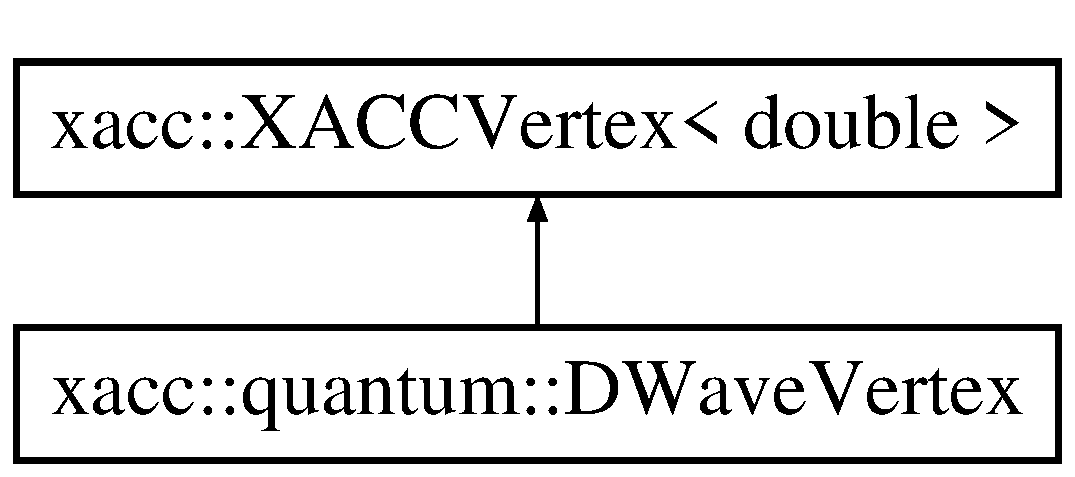
\includegraphics[height=2.000000cm]{a01256}
\end{center}
\end{figure}
\subsection*{Additional Inherited Members}


\subsection{Detailed Description}
The \hyperlink{a01256}{D\+Wave\+Vertex} is a subclass of the \hyperlink{a02516}{X\+A\+C\+C\+Vertex} that keeps track of one vertex parameter -\/ the qubit bias parameter. \hyperlink{a02516}{X\+A\+C\+C\+Vertex} already keeps track of edge weights. 

The documentation for this class was generated from the following file\+:\begin{DoxyCompactItemize}
\item 
Embedding\+Algorithm.\+hpp\end{DoxyCompactItemize}

\hypertarget{a01808}{}\section{fire\+:\+:Eigen\+Provider Class Reference}
\label{a01808}\index{fire\+::\+Eigen\+Provider@{fire\+::\+Eigen\+Provider}}


{\ttfamily \#include $<$Eigen\+Tensor\+Provider.\+hpp$>$}

Inheritance diagram for fire\+:\+:Eigen\+Provider\+:\begin{figure}[H]
\begin{center}
\leavevmode
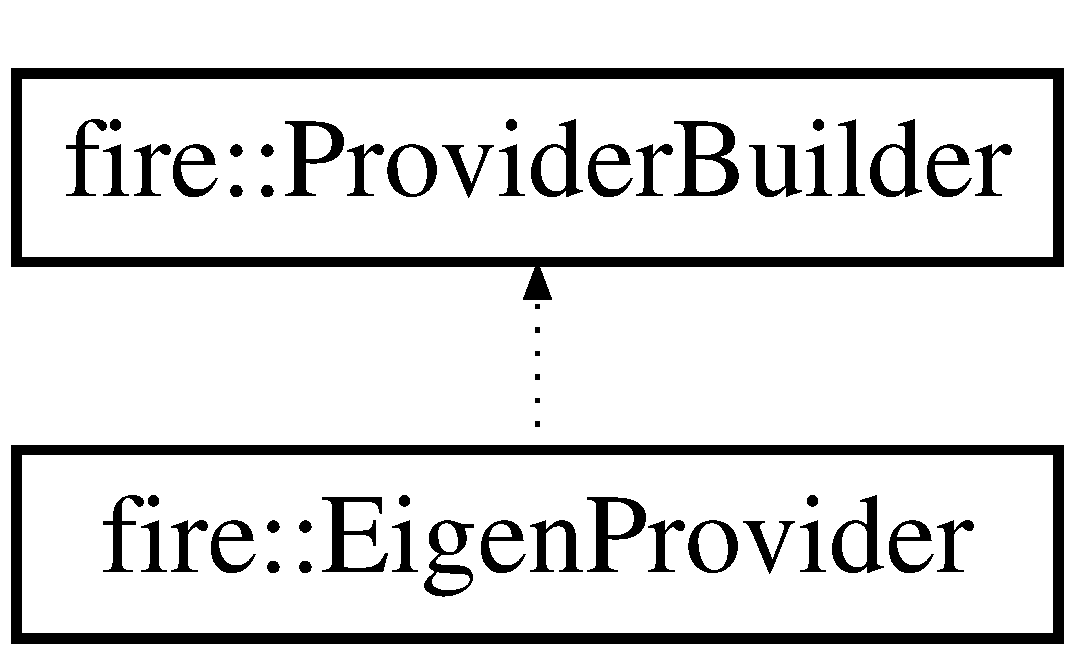
\includegraphics[height=2.000000cm]{a01808}
\end{center}
\end{figure}
\subsection*{Public Member Functions}
\begin{DoxyCompactItemize}
\item 
\mbox{\Hypertarget{a01808_ab9bfc7a0004ea10d57442f495c468b2e}\label{a01808_ab9bfc7a0004ea10d57442f495c468b2e}} 
{\footnotesize template$<$const int Rank, typename Scalar $>$ }\\\hyperlink{a01804}{Eigen\+Tensor\+Provider}$<$ Rank, Scalar $>$ {\bfseries build} ()
\end{DoxyCompactItemize}


\subsection{Detailed Description}
This class provides a mechanism for building Eigen\+Tensor\+Providers. It is used by the \hyperlink{a01812}{Tensor} class to appropriately construct a \hyperlink{a01816}{Tensor\+Provider} backed by Eigen Tensors. 

The documentation for this class was generated from the following file\+:\begin{DoxyCompactItemize}
\item 
Eigen\+Tensor\+Provider.\+hpp\end{DoxyCompactItemize}

\hypertarget{a01804}{}\section{fire\+:\+:Eigen\+Tensor\+Provider$<$ Rank, Scalar $>$ Class Template Reference}
\label{a01804}\index{fire\+::\+Eigen\+Tensor\+Provider$<$ Rank, Scalar $>$@{fire\+::\+Eigen\+Tensor\+Provider$<$ Rank, Scalar $>$}}


{\ttfamily \#include $<$Eigen\+Tensor\+Provider.\+hpp$>$}

Inheritance diagram for fire\+:\+:Eigen\+Tensor\+Provider$<$ Rank, Scalar $>$\+:\begin{figure}[H]
\begin{center}
\leavevmode
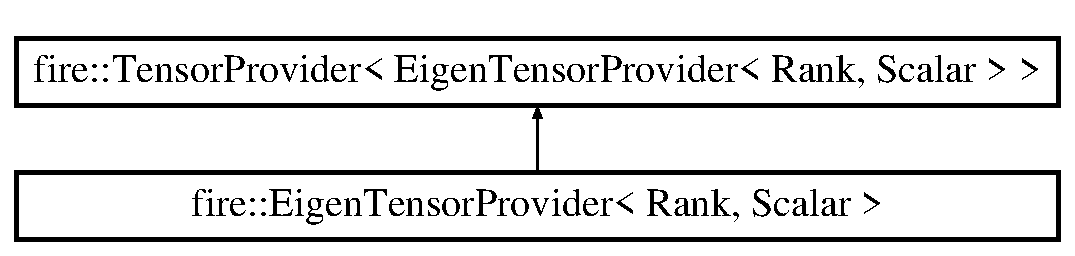
\includegraphics[height=2.000000cm]{a01804}
\end{center}
\end{figure}
\subsection*{Public Member Functions}
\begin{DoxyCompactItemize}
\item 
\hyperlink{a01804_a666937cbdec96978bdd47132a95ab9e6}{Eigen\+Tensor\+Provider} ()
\item 
{\footnotesize template$<$typename ... Dimensions$>$ }\\void \hyperlink{a01804_a5d7147962e2e85c0789b90cced1c6393}{initialize\+Tensor\+Backend} (int first\+Dim, Dimensions ... other\+Dims)
\item 
void \hyperlink{a01804_a284d6bb6a8539c5776e00d2a377d188e}{initialize\+Tensor\+Backend\+With\+Reference} (\hyperlink{a00648_a1bf491fd1c876e2808648b2fd291e3dd}{Tensor\+Reference}$<$ Scalar $>$ \&reference)
\item 
{\footnotesize template$<$typename ... Indices$>$ }\\Scalar \& \hyperlink{a01804_ab664a177792bfb39da25e92b88d6385a}{tensor\+Coefficient} (Indices ... indices)
\item 
bool \hyperlink{a01804_a3e15190363627f4c6b373dc56dd2b4f3}{check\+Equality} (\hyperlink{a00648_a1bf491fd1c876e2808648b2fd291e3dd}{Tensor\+Reference}$<$ Scalar $>$ \&other)
\item 
{\footnotesize template$<$typename Other\+Derived , typename Contraction\+Dims $>$ }\\\hyperlink{a00648_a1bf491fd1c876e2808648b2fd291e3dd}{Tensor\+Reference}$<$ Scalar $>$ \hyperlink{a01804_acd9f39dacb5fd6c35f3f840ed22194e9}{execute\+Contraction} (Other\+Derived \&t2, Contraction\+Dims \&c\+Indices)
\item 
Scalar $\ast$ \hyperlink{a01804_aff5626be9e55f593f0a6b71174ecbd8a}{data} ()
\item 
\hyperlink{a00648_a1bf491fd1c876e2808648b2fd291e3dd}{Tensor\+Reference}$<$ Scalar $>$ \hyperlink{a01804_a957d54e0259b1ea798a47389af4b8379}{add} (\hyperlink{a00648_a1bf491fd1c876e2808648b2fd291e3dd}{Tensor\+Reference}$<$ Scalar $>$ \&other)
\item 
{\footnotesize template$<$typename Init\+List $>$ }\\void \hyperlink{a01804_a3d02dbf7e2d255a1378084aa6459cf25}{set\+Tensor\+Values} (Init\+List \&vals)
\item 
void \hyperlink{a01804_a607ad28d9f0b8b7f639dc1b0693dfd03}{print\+Tensor} (std\+::ostream \&stream)
\item 
void \hyperlink{a01804_a461c3348c66ae011167d8c194c79dce9}{fill\+With\+Random\+Values} ()
\item 
\hyperlink{a00648_a1bf491fd1c876e2808648b2fd291e3dd}{Tensor\+Reference}$<$ Scalar $>$ \hyperlink{a01804_ae526f2376663adc8788ba8f4c04eb6cb}{scalar\+Product} (Scalar \&val)
\item 
{\footnotesize template$<$typename Dim\+Array $>$ }\\\hyperlink{a00648_a1bf491fd1c876e2808648b2fd291e3dd}{Tensor\+Reference}$<$ Scalar $>$ \hyperlink{a01804_a5ffd64a2a2a7b5886b2175d21a46dccf}{reshape\+Tensor} (Dim\+Array \&array)
\item 
\mbox{\Hypertarget{a01804_ac4d85c2ce0bfb666ddb7284241b74dcb}\label{a01804_ac4d85c2ce0bfb666ddb7284241b74dcb}} 
{\footnotesize template$<$typename Dim\+Array $>$ }\\\hyperlink{a00648_a1bf491fd1c876e2808648b2fd291e3dd}{Tensor\+Reference}$<$ Scalar $>$ {\bfseries shuffle\+Tensor} (Dim\+Array \&array)
\item 
\mbox{\Hypertarget{a01804_aa1ba881990a0af6e0a68f8927f94c89d}\label{a01804_aa1ba881990a0af6e0a68f8927f94c89d}} 
std\+::tuple$<$ \hyperlink{a00648_a1bf491fd1c876e2808648b2fd291e3dd}{Tensor\+Reference}$<$ Scalar $>$, \hyperlink{a00648_a1bf491fd1c876e2808648b2fd291e3dd}{Tensor\+Reference}$<$ Scalar $>$, \hyperlink{a00648_a1bf491fd1c876e2808648b2fd291e3dd}{Tensor\+Reference}$<$ Scalar $>$ $>$ {\bfseries compute\+Svd} (\hyperlink{a00648_a1bf491fd1c876e2808648b2fd291e3dd}{Tensor\+Reference}$<$ Scalar $>$ \&ref, double cutoff)
\item 
\mbox{\Hypertarget{a01804_ade4eea42a36aaa42cb8ea85ae3dee711}\label{a01804_ade4eea42a36aaa42cb8ea85ae3dee711}} 
\hyperlink{a00648_a1bf491fd1c876e2808648b2fd291e3dd}{Tensor\+Reference}$<$ Scalar $>$ {\bfseries kron\+Prod} (\hyperlink{a00648_a1bf491fd1c876e2808648b2fd291e3dd}{Tensor\+Reference}$<$ Scalar $>$ \&other)
\end{DoxyCompactItemize}
\subsection*{Static Public Member Functions}
\begin{DoxyCompactItemize}
\item 
static constexpr int \hyperlink{a01804_a68f0ad7ead91dec2ea56f173981465c8}{get\+Rank} ()
\end{DoxyCompactItemize}
\subsection*{Static Public Attributes}
\begin{DoxyCompactItemize}
\item 
static const int \hyperlink{a01804_ae8f0217985d78dba31d7bdb95ace1e43}{rank} = Rank
\end{DoxyCompactItemize}


\subsection{Detailed Description}
\subsubsection*{template$<$const int Rank, typename Scalar = double$>$\newline
class fire\+::\+Eigen\+Tensor\+Provider$<$ Rank, Scalar $>$}

The \hyperlink{a01804}{Eigen\+Tensor\+Provider} is a \hyperlink{a01816}{Tensor\+Provider} that provides tensor data and operations using the Eigen C++ tensor module. 

\subsection{Constructor \& Destructor Documentation}
\mbox{\Hypertarget{a01804_a666937cbdec96978bdd47132a95ab9e6}\label{a01804_a666937cbdec96978bdd47132a95ab9e6}} 
\index{fire\+::\+Eigen\+Tensor\+Provider@{fire\+::\+Eigen\+Tensor\+Provider}!Eigen\+Tensor\+Provider@{Eigen\+Tensor\+Provider}}
\index{Eigen\+Tensor\+Provider@{Eigen\+Tensor\+Provider}!fire\+::\+Eigen\+Tensor\+Provider@{fire\+::\+Eigen\+Tensor\+Provider}}
\subsubsection{\texorpdfstring{Eigen\+Tensor\+Provider()}{EigenTensorProvider()}}
{\footnotesize\ttfamily template$<$const int Rank, typename Scalar = double$>$ \\
\hyperlink{a01804}{fire\+::\+Eigen\+Tensor\+Provider}$<$ Rank, Scalar $>$\+::\hyperlink{a01804}{Eigen\+Tensor\+Provider} (\begin{DoxyParamCaption}{ }\end{DoxyParamCaption})\hspace{0.3cm}{\ttfamily [inline]}}

The Constructor 

\subsection{Member Function Documentation}
\mbox{\Hypertarget{a01804_a957d54e0259b1ea798a47389af4b8379}\label{a01804_a957d54e0259b1ea798a47389af4b8379}} 
\index{fire\+::\+Eigen\+Tensor\+Provider@{fire\+::\+Eigen\+Tensor\+Provider}!add@{add}}
\index{add@{add}!fire\+::\+Eigen\+Tensor\+Provider@{fire\+::\+Eigen\+Tensor\+Provider}}
\subsubsection{\texorpdfstring{add()}{add()}}
{\footnotesize\ttfamily template$<$const int Rank, typename Scalar = double$>$ \\
\hyperlink{a00648_a1bf491fd1c876e2808648b2fd291e3dd}{Tensor\+Reference}$<$Scalar$>$ \hyperlink{a01804}{fire\+::\+Eigen\+Tensor\+Provider}$<$ Rank, Scalar $>$\+::add (\begin{DoxyParamCaption}\item[{\hyperlink{a00648_a1bf491fd1c876e2808648b2fd291e3dd}{Tensor\+Reference}$<$ Scalar $>$ \&}]{other }\end{DoxyParamCaption})\hspace{0.3cm}{\ttfamily [inline]}}

Return a Tensor\+Reference representing the sum of this Eigen \hyperlink{a01812}{Tensor} and an Eigen \hyperlink{a01812}{Tensor} represented by the other Tensor\+Reference.


\begin{DoxyParams}{Parameters}
{\em other} & Tensor\+Reference view of the other \hyperlink{a01812}{Tensor} \\
\hline
\end{DoxyParams}
\begin{DoxyReturn}{Returns}
result A new Tensor\+Reference representing the sum of this and other. 
\end{DoxyReturn}
\mbox{\Hypertarget{a01804_a3e15190363627f4c6b373dc56dd2b4f3}\label{a01804_a3e15190363627f4c6b373dc56dd2b4f3}} 
\index{fire\+::\+Eigen\+Tensor\+Provider@{fire\+::\+Eigen\+Tensor\+Provider}!check\+Equality@{check\+Equality}}
\index{check\+Equality@{check\+Equality}!fire\+::\+Eigen\+Tensor\+Provider@{fire\+::\+Eigen\+Tensor\+Provider}}
\subsubsection{\texorpdfstring{check\+Equality()}{checkEquality()}}
{\footnotesize\ttfamily template$<$const int Rank, typename Scalar = double$>$ \\
bool \hyperlink{a01804}{fire\+::\+Eigen\+Tensor\+Provider}$<$ Rank, Scalar $>$\+::check\+Equality (\begin{DoxyParamCaption}\item[{\hyperlink{a00648_a1bf491fd1c876e2808648b2fd291e3dd}{Tensor\+Reference}$<$ Scalar $>$ \&}]{other }\end{DoxyParamCaption})\hspace{0.3cm}{\ttfamily [inline]}}

Return true if the provided Tensor\+Reference as a tensor is equal to this tensor.


\begin{DoxyParams}{Parameters}
{\em other} & Tensor\+Reference view of the other \hyperlink{a01812}{Tensor} \\
\hline
\end{DoxyParams}
\begin{DoxyReturn}{Returns}
equal A boolean indicating if these Tensors are equal 
\end{DoxyReturn}
\mbox{\Hypertarget{a01804_aff5626be9e55f593f0a6b71174ecbd8a}\label{a01804_aff5626be9e55f593f0a6b71174ecbd8a}} 
\index{fire\+::\+Eigen\+Tensor\+Provider@{fire\+::\+Eigen\+Tensor\+Provider}!data@{data}}
\index{data@{data}!fire\+::\+Eigen\+Tensor\+Provider@{fire\+::\+Eigen\+Tensor\+Provider}}
\subsubsection{\texorpdfstring{data()}{data()}}
{\footnotesize\ttfamily template$<$const int Rank, typename Scalar = double$>$ \\
Scalar$\ast$ \hyperlink{a01804}{fire\+::\+Eigen\+Tensor\+Provider}$<$ Rank, Scalar $>$\+::data (\begin{DoxyParamCaption}{ }\end{DoxyParamCaption})\hspace{0.3cm}{\ttfamily [inline]}}

Return the 1-\/D array wrapped by this Eigen \hyperlink{a01812}{Tensor}

\begin{DoxyReturn}{Returns}
data 1-\/D array of data representing the tensor in this \hyperlink{a01816}{Tensor\+Provider} 
\end{DoxyReturn}
\mbox{\Hypertarget{a01804_acd9f39dacb5fd6c35f3f840ed22194e9}\label{a01804_acd9f39dacb5fd6c35f3f840ed22194e9}} 
\index{fire\+::\+Eigen\+Tensor\+Provider@{fire\+::\+Eigen\+Tensor\+Provider}!execute\+Contraction@{execute\+Contraction}}
\index{execute\+Contraction@{execute\+Contraction}!fire\+::\+Eigen\+Tensor\+Provider@{fire\+::\+Eigen\+Tensor\+Provider}}
\subsubsection{\texorpdfstring{execute\+Contraction()}{executeContraction()}}
{\footnotesize\ttfamily template$<$const int Rank, typename Scalar = double$>$ \\
template$<$typename Other\+Derived , typename Contraction\+Dims $>$ \\
\hyperlink{a00648_a1bf491fd1c876e2808648b2fd291e3dd}{Tensor\+Reference}$<$Scalar$>$ \hyperlink{a01804}{fire\+::\+Eigen\+Tensor\+Provider}$<$ Rank, Scalar $>$\+::execute\+Contraction (\begin{DoxyParamCaption}\item[{Other\+Derived \&}]{t2,  }\item[{Contraction\+Dims \&}]{c\+Indices }\end{DoxyParamCaption})\hspace{0.3cm}{\ttfamily [inline]}}

Compute the tensor contraction of this Eigen \hyperlink{a01812}{Tensor} with the provided Other \hyperlink{a01812}{Tensor}.


\begin{DoxyParams}{Parameters}
{\em t2} & The other \hyperlink{a01812}{Tensor} \\
\hline
{\em indices} & The contraction indices. \\
\hline
\end{DoxyParams}
\begin{DoxyReturn}{Returns}
result The contraction result as a Tensor\+Reference 
\end{DoxyReturn}
\mbox{\Hypertarget{a01804_a461c3348c66ae011167d8c194c79dce9}\label{a01804_a461c3348c66ae011167d8c194c79dce9}} 
\index{fire\+::\+Eigen\+Tensor\+Provider@{fire\+::\+Eigen\+Tensor\+Provider}!fill\+With\+Random\+Values@{fill\+With\+Random\+Values}}
\index{fill\+With\+Random\+Values@{fill\+With\+Random\+Values}!fire\+::\+Eigen\+Tensor\+Provider@{fire\+::\+Eigen\+Tensor\+Provider}}
\subsubsection{\texorpdfstring{fill\+With\+Random\+Values()}{fillWithRandomValues()}}
{\footnotesize\ttfamily template$<$const int Rank, typename Scalar = double$>$ \\
void \hyperlink{a01804}{fire\+::\+Eigen\+Tensor\+Provider}$<$ Rank, Scalar $>$\+::fill\+With\+Random\+Values (\begin{DoxyParamCaption}{ }\end{DoxyParamCaption})\hspace{0.3cm}{\ttfamily [inline]}}

Set the Eigen \hyperlink{a01812}{Tensor} values to random values. \mbox{\Hypertarget{a01804_a68f0ad7ead91dec2ea56f173981465c8}\label{a01804_a68f0ad7ead91dec2ea56f173981465c8}} 
\index{fire\+::\+Eigen\+Tensor\+Provider@{fire\+::\+Eigen\+Tensor\+Provider}!get\+Rank@{get\+Rank}}
\index{get\+Rank@{get\+Rank}!fire\+::\+Eigen\+Tensor\+Provider@{fire\+::\+Eigen\+Tensor\+Provider}}
\subsubsection{\texorpdfstring{get\+Rank()}{getRank()}}
{\footnotesize\ttfamily template$<$const int Rank, typename Scalar = double$>$ \\
static constexpr int \hyperlink{a01804}{fire\+::\+Eigen\+Tensor\+Provider}$<$ Rank, Scalar $>$\+::get\+Rank (\begin{DoxyParamCaption}{ }\end{DoxyParamCaption})\hspace{0.3cm}{\ttfamily [inline]}, {\ttfamily [static]}}

Return the rank of this Eigen \hyperlink{a01812}{Tensor}

\begin{DoxyReturn}{Returns}
rank The rank of this \hyperlink{a01812}{Tensor} 
\end{DoxyReturn}
\mbox{\Hypertarget{a01804_a5d7147962e2e85c0789b90cced1c6393}\label{a01804_a5d7147962e2e85c0789b90cced1c6393}} 
\index{fire\+::\+Eigen\+Tensor\+Provider@{fire\+::\+Eigen\+Tensor\+Provider}!initialize\+Tensor\+Backend@{initialize\+Tensor\+Backend}}
\index{initialize\+Tensor\+Backend@{initialize\+Tensor\+Backend}!fire\+::\+Eigen\+Tensor\+Provider@{fire\+::\+Eigen\+Tensor\+Provider}}
\subsubsection{\texorpdfstring{initialize\+Tensor\+Backend()}{initializeTensorBackend()}}
{\footnotesize\ttfamily template$<$const int Rank, typename Scalar = double$>$ \\
template$<$typename ... Dimensions$>$ \\
void \hyperlink{a01804}{fire\+::\+Eigen\+Tensor\+Provider}$<$ Rank, Scalar $>$\+::initialize\+Tensor\+Backend (\begin{DoxyParamCaption}\item[{int}]{first\+Dim,  }\item[{Dimensions ...}]{other\+Dims }\end{DoxyParamCaption})\hspace{0.3cm}{\ttfamily [inline]}}

Initialize the Eigen \hyperlink{a01812}{Tensor} with all zeros. 
\begin{DoxyParams}{Parameters}
{\em first\+Dim} & \\
\hline
{\em other\+Dims} & \\
\hline
\end{DoxyParams}
\mbox{\Hypertarget{a01804_a284d6bb6a8539c5776e00d2a377d188e}\label{a01804_a284d6bb6a8539c5776e00d2a377d188e}} 
\index{fire\+::\+Eigen\+Tensor\+Provider@{fire\+::\+Eigen\+Tensor\+Provider}!initialize\+Tensor\+Backend\+With\+Reference@{initialize\+Tensor\+Backend\+With\+Reference}}
\index{initialize\+Tensor\+Backend\+With\+Reference@{initialize\+Tensor\+Backend\+With\+Reference}!fire\+::\+Eigen\+Tensor\+Provider@{fire\+::\+Eigen\+Tensor\+Provider}}
\subsubsection{\texorpdfstring{initialize\+Tensor\+Backend\+With\+Reference()}{initializeTensorBackendWithReference()}}
{\footnotesize\ttfamily template$<$const int Rank, typename Scalar = double$>$ \\
void \hyperlink{a01804}{fire\+::\+Eigen\+Tensor\+Provider}$<$ Rank, Scalar $>$\+::initialize\+Tensor\+Backend\+With\+Reference (\begin{DoxyParamCaption}\item[{\hyperlink{a00648_a1bf491fd1c876e2808648b2fd291e3dd}{Tensor\+Reference}$<$ Scalar $>$ \&}]{reference }\end{DoxyParamCaption})\hspace{0.3cm}{\ttfamily [inline]}}

Initialize the Eigen \hyperlink{a01812}{Tensor} from an existing Tensor\+Reference 
\begin{DoxyParams}{Parameters}
{\em reference} & \\
\hline
\end{DoxyParams}
\mbox{\Hypertarget{a01804_a607ad28d9f0b8b7f639dc1b0693dfd03}\label{a01804_a607ad28d9f0b8b7f639dc1b0693dfd03}} 
\index{fire\+::\+Eigen\+Tensor\+Provider@{fire\+::\+Eigen\+Tensor\+Provider}!print\+Tensor@{print\+Tensor}}
\index{print\+Tensor@{print\+Tensor}!fire\+::\+Eigen\+Tensor\+Provider@{fire\+::\+Eigen\+Tensor\+Provider}}
\subsubsection{\texorpdfstring{print\+Tensor()}{printTensor()}}
{\footnotesize\ttfamily template$<$const int Rank, typename Scalar = double$>$ \\
void \hyperlink{a01804}{fire\+::\+Eigen\+Tensor\+Provider}$<$ Rank, Scalar $>$\+::print\+Tensor (\begin{DoxyParamCaption}\item[{std\+::ostream \&}]{stream }\end{DoxyParamCaption})\hspace{0.3cm}{\ttfamily [inline]}}

Output this Eigen \hyperlink{a01812}{Tensor} to the provided output stream.


\begin{DoxyParams}{Parameters}
{\em output\+Stream} & The output stream to write the tensor to. \\
\hline
\end{DoxyParams}
\mbox{\Hypertarget{a01804_a5ffd64a2a2a7b5886b2175d21a46dccf}\label{a01804_a5ffd64a2a2a7b5886b2175d21a46dccf}} 
\index{fire\+::\+Eigen\+Tensor\+Provider@{fire\+::\+Eigen\+Tensor\+Provider}!reshape\+Tensor@{reshape\+Tensor}}
\index{reshape\+Tensor@{reshape\+Tensor}!fire\+::\+Eigen\+Tensor\+Provider@{fire\+::\+Eigen\+Tensor\+Provider}}
\subsubsection{\texorpdfstring{reshape\+Tensor()}{reshapeTensor()}}
{\footnotesize\ttfamily template$<$const int Rank, typename Scalar = double$>$ \\
template$<$typename Dim\+Array $>$ \\
\hyperlink{a00648_a1bf491fd1c876e2808648b2fd291e3dd}{Tensor\+Reference}$<$Scalar$>$ \hyperlink{a01804}{fire\+::\+Eigen\+Tensor\+Provider}$<$ Rank, Scalar $>$\+::reshape\+Tensor (\begin{DoxyParamCaption}\item[{Dim\+Array \&}]{array }\end{DoxyParamCaption})\hspace{0.3cm}{\ttfamily [inline]}}

Reshape the Eigen \hyperlink{a01812}{Tensor} with a new array of dimensions


\begin{DoxyParams}{Parameters}
{\em array} & Array of new dimensions for each rank index \\
\hline
\end{DoxyParams}
\begin{DoxyReturn}{Returns}
reshaped\+Tensor A Tensor\+Reference representing new reshaped tensor. 
\end{DoxyReturn}
\mbox{\Hypertarget{a01804_ae526f2376663adc8788ba8f4c04eb6cb}\label{a01804_ae526f2376663adc8788ba8f4c04eb6cb}} 
\index{fire\+::\+Eigen\+Tensor\+Provider@{fire\+::\+Eigen\+Tensor\+Provider}!scalar\+Product@{scalar\+Product}}
\index{scalar\+Product@{scalar\+Product}!fire\+::\+Eigen\+Tensor\+Provider@{fire\+::\+Eigen\+Tensor\+Provider}}
\subsubsection{\texorpdfstring{scalar\+Product()}{scalarProduct()}}
{\footnotesize\ttfamily template$<$const int Rank, typename Scalar = double$>$ \\
\hyperlink{a00648_a1bf491fd1c876e2808648b2fd291e3dd}{Tensor\+Reference}$<$Scalar$>$ \hyperlink{a01804}{fire\+::\+Eigen\+Tensor\+Provider}$<$ Rank, Scalar $>$\+::scalar\+Product (\begin{DoxyParamCaption}\item[{Scalar \&}]{val }\end{DoxyParamCaption})\hspace{0.3cm}{\ttfamily [inline]}}

Multiply all elements of this Eigen \hyperlink{a01812}{Tensor} by the provided Scalar.


\begin{DoxyParams}{Parameters}
{\em val} & Scalar to multiply this tensor by. \\
\hline
\end{DoxyParams}
\begin{DoxyReturn}{Returns}
result A Tensor\+Reference representing the result 
\end{DoxyReturn}
\mbox{\Hypertarget{a01804_a3d02dbf7e2d255a1378084aa6459cf25}\label{a01804_a3d02dbf7e2d255a1378084aa6459cf25}} 
\index{fire\+::\+Eigen\+Tensor\+Provider@{fire\+::\+Eigen\+Tensor\+Provider}!set\+Tensor\+Values@{set\+Tensor\+Values}}
\index{set\+Tensor\+Values@{set\+Tensor\+Values}!fire\+::\+Eigen\+Tensor\+Provider@{fire\+::\+Eigen\+Tensor\+Provider}}
\subsubsection{\texorpdfstring{set\+Tensor\+Values()}{setTensorValues()}}
{\footnotesize\ttfamily template$<$const int Rank, typename Scalar = double$>$ \\
template$<$typename Init\+List $>$ \\
void \hyperlink{a01804}{fire\+::\+Eigen\+Tensor\+Provider}$<$ Rank, Scalar $>$\+::set\+Tensor\+Values (\begin{DoxyParamCaption}\item[{Init\+List \&}]{vals }\end{DoxyParamCaption})\hspace{0.3cm}{\ttfamily [inline]}}

Set the Eigen \hyperlink{a01812}{Tensor} values using nested initializer\+\_\+list


\begin{DoxyParams}{Parameters}
{\em vals} & The values as a nest std\+::initializer\+\_\+lists \\
\hline
\end{DoxyParams}
\mbox{\Hypertarget{a01804_ab664a177792bfb39da25e92b88d6385a}\label{a01804_ab664a177792bfb39da25e92b88d6385a}} 
\index{fire\+::\+Eigen\+Tensor\+Provider@{fire\+::\+Eigen\+Tensor\+Provider}!tensor\+Coefficient@{tensor\+Coefficient}}
\index{tensor\+Coefficient@{tensor\+Coefficient}!fire\+::\+Eigen\+Tensor\+Provider@{fire\+::\+Eigen\+Tensor\+Provider}}
\subsubsection{\texorpdfstring{tensor\+Coefficient()}{tensorCoefficient()}}
{\footnotesize\ttfamily template$<$const int Rank, typename Scalar = double$>$ \\
template$<$typename ... Indices$>$ \\
Scalar\& \hyperlink{a01804}{fire\+::\+Eigen\+Tensor\+Provider}$<$ Rank, Scalar $>$\+::tensor\+Coefficient (\begin{DoxyParamCaption}\item[{Indices ...}]{indices }\end{DoxyParamCaption})\hspace{0.3cm}{\ttfamily [inline]}}

Return the coefficient at the given tensor indices.


\begin{DoxyParams}{Parameters}
{\em indices} & The indices for the desired value \\
\hline
\end{DoxyParams}
\begin{DoxyReturn}{Returns}
val The value at the indices. 
\end{DoxyReturn}


\subsection{Member Data Documentation}
\mbox{\Hypertarget{a01804_ae8f0217985d78dba31d7bdb95ace1e43}\label{a01804_ae8f0217985d78dba31d7bdb95ace1e43}} 
\index{fire\+::\+Eigen\+Tensor\+Provider@{fire\+::\+Eigen\+Tensor\+Provider}!rank@{rank}}
\index{rank@{rank}!fire\+::\+Eigen\+Tensor\+Provider@{fire\+::\+Eigen\+Tensor\+Provider}}
\subsubsection{\texorpdfstring{rank}{rank}}
{\footnotesize\ttfamily template$<$const int Rank, typename Scalar = double$>$ \\
const int \hyperlink{a01804}{fire\+::\+Eigen\+Tensor\+Provider}$<$ Rank, Scalar $>$\+::rank = Rank\hspace{0.3cm}{\ttfamily [static]}}

Static reference to the rank of the tensor wrapped by this provider 

The documentation for this class was generated from the following file\+:\begin{DoxyCompactItemize}
\item 
Eigen\+Tensor\+Provider.\+hpp\end{DoxyCompactItemize}

\hypertarget{a01388}{}\section{boost\+:\+:dll\+:\+:detail\+:\+:Elf\+\_\+\+Ehdr\+\_\+template$<$ Address\+OffsetT $>$ Struct Template Reference}
\label{a01388}\index{boost\+::dll\+::detail\+::\+Elf\+\_\+\+Ehdr\+\_\+template$<$ Address\+Offset\+T $>$@{boost\+::dll\+::detail\+::\+Elf\+\_\+\+Ehdr\+\_\+template$<$ Address\+Offset\+T $>$}}
\subsection*{Public Attributes}
\begin{DoxyCompactItemize}
\item 
\mbox{\Hypertarget{a01388_abd8c4939b91291c458036b4807e42f44}\label{a01388_abd8c4939b91291c458036b4807e42f44}} 
unsigned char {\bfseries e\+\_\+ident} \mbox{[}16\mbox{]}
\item 
\mbox{\Hypertarget{a01388_ad761c6ff499b8981693c43d55878e9a1}\label{a01388_ad761c6ff499b8981693c43d55878e9a1}} 
boost\+::uint16\+\_\+t {\bfseries e\+\_\+type}
\item 
\mbox{\Hypertarget{a01388_aae3b4d52bdf89e04371782ba642ce281}\label{a01388_aae3b4d52bdf89e04371782ba642ce281}} 
boost\+::uint16\+\_\+t {\bfseries e\+\_\+machine}
\item 
\mbox{\Hypertarget{a01388_a96cddf93afbcbbc9830713f26ce02b5a}\label{a01388_a96cddf93afbcbbc9830713f26ce02b5a}} 
boost\+::uint32\+\_\+t {\bfseries e\+\_\+version}
\item 
\mbox{\Hypertarget{a01388_a332c4575e5f2e605dc877175929aba24}\label{a01388_a332c4575e5f2e605dc877175929aba24}} 
Address\+OffsetT {\bfseries e\+\_\+entry}
\item 
\mbox{\Hypertarget{a01388_aa3b51c343127152028891c427f36c96c}\label{a01388_aa3b51c343127152028891c427f36c96c}} 
Address\+OffsetT {\bfseries e\+\_\+phoff}
\item 
\mbox{\Hypertarget{a01388_a8a02464e0684454b89bc0124a87fee6f}\label{a01388_a8a02464e0684454b89bc0124a87fee6f}} 
Address\+OffsetT {\bfseries e\+\_\+shoff}
\item 
\mbox{\Hypertarget{a01388_a371d9ac16582e3c32defb575809892f6}\label{a01388_a371d9ac16582e3c32defb575809892f6}} 
boost\+::uint32\+\_\+t {\bfseries e\+\_\+flags}
\item 
\mbox{\Hypertarget{a01388_aa3887c3b940f630dbb78807f8cc81c82}\label{a01388_aa3887c3b940f630dbb78807f8cc81c82}} 
boost\+::uint16\+\_\+t {\bfseries e\+\_\+ehsize}
\item 
\mbox{\Hypertarget{a01388_aae8978ff0f2a20896b3c1ed34dc0793e}\label{a01388_aae8978ff0f2a20896b3c1ed34dc0793e}} 
boost\+::uint16\+\_\+t {\bfseries e\+\_\+phentsize}
\item 
\mbox{\Hypertarget{a01388_af1962363e104e15e4635066806e52a00}\label{a01388_af1962363e104e15e4635066806e52a00}} 
boost\+::uint16\+\_\+t {\bfseries e\+\_\+phnum}
\item 
\mbox{\Hypertarget{a01388_a9d22ea8279a4c31365059d2ebe3bac56}\label{a01388_a9d22ea8279a4c31365059d2ebe3bac56}} 
boost\+::uint16\+\_\+t {\bfseries e\+\_\+shentsize}
\item 
\mbox{\Hypertarget{a01388_a610b772eda5456c9a9ab83537caef750}\label{a01388_a610b772eda5456c9a9ab83537caef750}} 
boost\+::uint16\+\_\+t {\bfseries e\+\_\+shnum}
\item 
\mbox{\Hypertarget{a01388_acae2be4b1e8d9766b5f9aaf32d5e7ca4}\label{a01388_acae2be4b1e8d9766b5f9aaf32d5e7ca4}} 
boost\+::uint16\+\_\+t {\bfseries e\+\_\+shstrndx}
\end{DoxyCompactItemize}


The documentation for this struct was generated from the following file\+:\begin{DoxyCompactItemize}
\item 
elf\+\_\+info.\+hpp\end{DoxyCompactItemize}

\hypertarget{a01408}{}\section{boost\+:\+:dll\+:\+:detail\+:\+:elf\+\_\+info$<$ Address\+OffsetT $>$ Class Template Reference}
\label{a01408}\index{boost\+::dll\+::detail\+::elf\+\_\+info$<$ Address\+Offset\+T $>$@{boost\+::dll\+::detail\+::elf\+\_\+info$<$ Address\+Offset\+T $>$}}
Inheritance diagram for boost\+:\+:dll\+:\+:detail\+:\+:elf\+\_\+info$<$ Address\+OffsetT $>$\+:\begin{figure}[H]
\begin{center}
\leavevmode
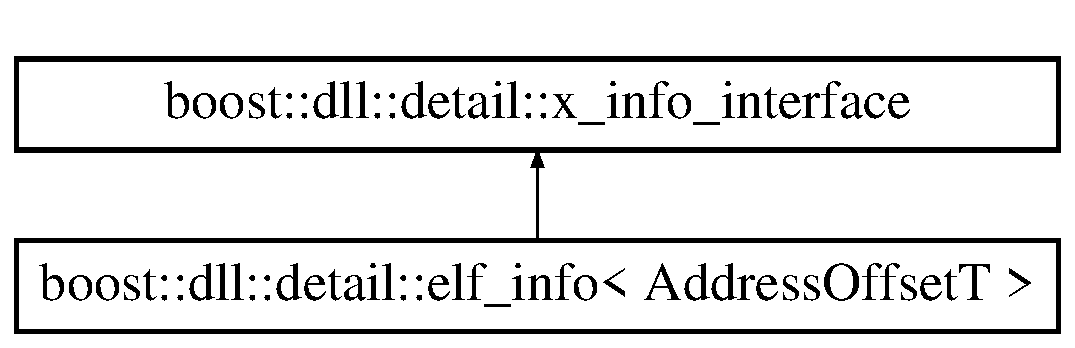
\includegraphics[height=2.000000cm]{a01408}
\end{center}
\end{figure}
\subsection*{Public Member Functions}
\begin{DoxyCompactItemize}
\item 
\mbox{\Hypertarget{a01408_a86ac2d6ccd8f1690d9fa285a20a9357e}\label{a01408_a86ac2d6ccd8f1690d9fa285a20a9357e}} 
{\bfseries elf\+\_\+info} (boost\+::filesystem\+::ifstream \&f) B\+O\+O\+S\+T\+\_\+\+N\+O\+E\+X\+C\+E\+PT
\item 
\mbox{\Hypertarget{a01408_a14b62434f2be710f2a0a8da8fde24bca}\label{a01408_a14b62434f2be710f2a0a8da8fde24bca}} 
std\+::vector$<$ std\+::string $>$ {\bfseries sections} ()
\item 
\mbox{\Hypertarget{a01408_a131b0f293d358d4d75ac6f63ec365285}\label{a01408_a131b0f293d358d4d75ac6f63ec365285}} 
std\+::vector$<$ std\+::string $>$ {\bfseries symbols} ()
\item 
\mbox{\Hypertarget{a01408_a07e28e88baa3914a205693b8921d2b87}\label{a01408_a07e28e88baa3914a205693b8921d2b87}} 
std\+::vector$<$ std\+::string $>$ {\bfseries symbols} (const char $\ast$section\+\_\+name)
\end{DoxyCompactItemize}
\subsection*{Static Public Member Functions}
\begin{DoxyCompactItemize}
\item 
\mbox{\Hypertarget{a01408_a7f38916fd4bb133614d04870406d7c62}\label{a01408_a7f38916fd4bb133614d04870406d7c62}} 
static bool {\bfseries parsing\+\_\+supported} (boost\+::filesystem\+::ifstream \&f)
\end{DoxyCompactItemize}


The documentation for this class was generated from the following file\+:\begin{DoxyCompactItemize}
\item 
elf\+\_\+info.\+hpp\end{DoxyCompactItemize}

\hypertarget{a01392}{}\section{boost\+:\+:dll\+:\+:detail\+:\+:Elf\+\_\+\+Shdr\+\_\+template$<$ Address\+OffsetT $>$ Struct Template Reference}
\label{a01392}\index{boost\+::dll\+::detail\+::\+Elf\+\_\+\+Shdr\+\_\+template$<$ Address\+Offset\+T $>$@{boost\+::dll\+::detail\+::\+Elf\+\_\+\+Shdr\+\_\+template$<$ Address\+Offset\+T $>$}}
\subsection*{Public Attributes}
\begin{DoxyCompactItemize}
\item 
\mbox{\Hypertarget{a01392_af74b85fd375874942acab42fb236938b}\label{a01392_af74b85fd375874942acab42fb236938b}} 
boost\+::uint32\+\_\+t {\bfseries sh\+\_\+name}
\item 
\mbox{\Hypertarget{a01392_aef81ee9415e932f037457039ecb6062a}\label{a01392_aef81ee9415e932f037457039ecb6062a}} 
boost\+::uint32\+\_\+t {\bfseries sh\+\_\+type}
\item 
\mbox{\Hypertarget{a01392_a0cf665258d1353d703dbe5f03b06377c}\label{a01392_a0cf665258d1353d703dbe5f03b06377c}} 
Address\+OffsetT {\bfseries sh\+\_\+flags}
\item 
\mbox{\Hypertarget{a01392_a96484407d371204d2cdf512c946a3035}\label{a01392_a96484407d371204d2cdf512c946a3035}} 
Address\+OffsetT {\bfseries sh\+\_\+addr}
\item 
\mbox{\Hypertarget{a01392_a218d431d671c785239cbe32d5f566329}\label{a01392_a218d431d671c785239cbe32d5f566329}} 
Address\+OffsetT {\bfseries sh\+\_\+offset}
\item 
\mbox{\Hypertarget{a01392_a0e8fbbadfb65a2c456951a632a114b0f}\label{a01392_a0e8fbbadfb65a2c456951a632a114b0f}} 
Address\+OffsetT {\bfseries sh\+\_\+size}
\item 
\mbox{\Hypertarget{a01392_a0f3c4d6a3f6db4ce3debe84bfab65aa4}\label{a01392_a0f3c4d6a3f6db4ce3debe84bfab65aa4}} 
boost\+::uint32\+\_\+t {\bfseries sh\+\_\+link}
\item 
\mbox{\Hypertarget{a01392_ab2ae82258ef53873e52f5711efd46f69}\label{a01392_ab2ae82258ef53873e52f5711efd46f69}} 
boost\+::uint32\+\_\+t {\bfseries sh\+\_\+info}
\item 
\mbox{\Hypertarget{a01392_a8b78c53bdbdd717f69a20f53427d99d5}\label{a01392_a8b78c53bdbdd717f69a20f53427d99d5}} 
Address\+OffsetT {\bfseries sh\+\_\+addralign}
\item 
\mbox{\Hypertarget{a01392_a736b1d41e2034475f8dcf3119614e88d}\label{a01392_a736b1d41e2034475f8dcf3119614e88d}} 
Address\+OffsetT {\bfseries sh\+\_\+entsize}
\end{DoxyCompactItemize}


The documentation for this struct was generated from the following file\+:\begin{DoxyCompactItemize}
\item 
elf\+\_\+info.\+hpp\end{DoxyCompactItemize}

\hypertarget{a01396}{}\section{boost\+:\+:dll\+:\+:detail\+:\+:Elf\+\_\+\+Sym\+\_\+template$<$ Address\+OffsetT $>$ Struct Template Reference}
\label{a01396}\index{boost\+::dll\+::detail\+::\+Elf\+\_\+\+Sym\+\_\+template$<$ Address\+Offset\+T $>$@{boost\+::dll\+::detail\+::\+Elf\+\_\+\+Sym\+\_\+template$<$ Address\+Offset\+T $>$}}


The documentation for this struct was generated from the following file\+:\begin{DoxyCompactItemize}
\item 
elf\+\_\+info.\+hpp\end{DoxyCompactItemize}

\hypertarget{a01400}{}\section{boost\+:\+:dll\+:\+:detail\+:\+:Elf\+\_\+\+Sym\+\_\+template$<$ boost\+:\+:uint32\+\_\+t $>$ Struct Template Reference}
\label{a01400}\index{boost\+::dll\+::detail\+::\+Elf\+\_\+\+Sym\+\_\+template$<$ boost\+::uint32\+\_\+t $>$@{boost\+::dll\+::detail\+::\+Elf\+\_\+\+Sym\+\_\+template$<$ boost\+::uint32\+\_\+t $>$}}
\subsection*{Public Types}
\begin{DoxyCompactItemize}
\item 
\mbox{\Hypertarget{a01400_a5d357c24b88c12797825ae9aac2ad518}\label{a01400_a5d357c24b88c12797825ae9aac2ad518}} 
typedef boost\+::uint32\+\_\+t {\bfseries Address\+OffsetT}
\end{DoxyCompactItemize}
\subsection*{Public Attributes}
\begin{DoxyCompactItemize}
\item 
\mbox{\Hypertarget{a01400_a5f05cce584bc27a780fe9d1526c819c3}\label{a01400_a5f05cce584bc27a780fe9d1526c819c3}} 
boost\+::uint32\+\_\+t {\bfseries st\+\_\+name}
\item 
\mbox{\Hypertarget{a01400_a22d87bb002a00dfaf68e38618b08e972}\label{a01400_a22d87bb002a00dfaf68e38618b08e972}} 
Address\+OffsetT {\bfseries st\+\_\+value}
\item 
\mbox{\Hypertarget{a01400_a8ad90ebe03f73b3d89493d5d454fffdf}\label{a01400_a8ad90ebe03f73b3d89493d5d454fffdf}} 
Address\+OffsetT {\bfseries st\+\_\+size}
\item 
\mbox{\Hypertarget{a01400_a4c025e263be3687bc20e584ec187786c}\label{a01400_a4c025e263be3687bc20e584ec187786c}} 
unsigned char {\bfseries st\+\_\+info}
\item 
\mbox{\Hypertarget{a01400_ac583a35bd53e3e45c0da77d2b7de504f}\label{a01400_ac583a35bd53e3e45c0da77d2b7de504f}} 
unsigned char {\bfseries st\+\_\+other}
\item 
\mbox{\Hypertarget{a01400_ac782cc2b5aac3204a6553d3534e112dd}\label{a01400_ac782cc2b5aac3204a6553d3534e112dd}} 
boost\+::uint16\+\_\+t {\bfseries st\+\_\+shndx}
\end{DoxyCompactItemize}


The documentation for this struct was generated from the following file\+:\begin{DoxyCompactItemize}
\item 
elf\+\_\+info.\+hpp\end{DoxyCompactItemize}

\hypertarget{a01404}{}\section{boost\+:\+:dll\+:\+:detail\+:\+:Elf\+\_\+\+Sym\+\_\+template$<$ boost\+:\+:uint64\+\_\+t $>$ Struct Template Reference}
\label{a01404}\index{boost\+::dll\+::detail\+::\+Elf\+\_\+\+Sym\+\_\+template$<$ boost\+::uint64\+\_\+t $>$@{boost\+::dll\+::detail\+::\+Elf\+\_\+\+Sym\+\_\+template$<$ boost\+::uint64\+\_\+t $>$}}
\subsection*{Public Types}
\begin{DoxyCompactItemize}
\item 
\mbox{\Hypertarget{a01404_ad1e44aba1f99d966aa2709e3bdcd47fe}\label{a01404_ad1e44aba1f99d966aa2709e3bdcd47fe}} 
typedef boost\+::uint64\+\_\+t {\bfseries Address\+OffsetT}
\end{DoxyCompactItemize}
\subsection*{Public Attributes}
\begin{DoxyCompactItemize}
\item 
\mbox{\Hypertarget{a01404_a622647e816f59015eafe01228113a646}\label{a01404_a622647e816f59015eafe01228113a646}} 
boost\+::uint32\+\_\+t {\bfseries st\+\_\+name}
\item 
\mbox{\Hypertarget{a01404_ae28b231a04d45e9e22039be6bc174b60}\label{a01404_ae28b231a04d45e9e22039be6bc174b60}} 
unsigned char {\bfseries st\+\_\+info}
\item 
\mbox{\Hypertarget{a01404_aff5bd6040881e1411f92650ce08fff84}\label{a01404_aff5bd6040881e1411f92650ce08fff84}} 
unsigned char {\bfseries st\+\_\+other}
\item 
\mbox{\Hypertarget{a01404_ac6f0b6c91c7c5e9ce4c4ef6e8adbf284}\label{a01404_ac6f0b6c91c7c5e9ce4c4ef6e8adbf284}} 
boost\+::uint16\+\_\+t {\bfseries st\+\_\+shndx}
\item 
\mbox{\Hypertarget{a01404_aa4e2698ae197ce1df4a7ea931e075cd6}\label{a01404_aa4e2698ae197ce1df4a7ea931e075cd6}} 
Address\+OffsetT {\bfseries st\+\_\+value}
\item 
\mbox{\Hypertarget{a01404_a6c32a90249fb0b6c430075634bfc5db1}\label{a01404_a6c32a90249fb0b6c430075634bfc5db1}} 
Address\+OffsetT {\bfseries st\+\_\+size}
\end{DoxyCompactItemize}


The documentation for this struct was generated from the following file\+:\begin{DoxyCompactItemize}
\item 
elf\+\_\+info.\+hpp\end{DoxyCompactItemize}

\hypertarget{a01260}{}\section{xacc\+:\+:quantum\+:\+:Embedding\+Algorithm Class Reference}
\label{a01260}\index{xacc\+::quantum\+::\+Embedding\+Algorithm@{xacc\+::quantum\+::\+Embedding\+Algorithm}}


{\ttfamily \#include $<$Embedding\+Algorithm.\+hpp$>$}

\subsection*{Public Member Functions}
\begin{DoxyCompactItemize}
\item 
\hyperlink{a01260_abad06507eef6b63af0884e3a96145c69}{Embedding\+Algorithm} ()
\item 
virtual \hyperlink{a01260_aa43660ad5d4c4b3ac67863892c33dc51}{$\sim$\+Embedding\+Algorithm} ()
\item 
virtual std\+::map$<$ int, std\+::list$<$ int $>$ $>$ \hyperlink{a01260_a67158c0f4925ff6b85698efec61e1175}{embed} (std\+::shared\+\_\+ptr$<$ \hyperlink{a02528}{D\+Wave\+Graph} $>$ problem, std\+::shared\+\_\+ptr$<$ \hyperlink{a02528}{D\+Wave\+Graph} $>$ hardware, std\+::map$<$ std\+::string, std\+::string $>$ params=std\+::map$<$ std\+::string, std\+::string $>$())=0
\item 
virtual std\+::string \hyperlink{a01260_a21079dc8ee37792977f5fd209e3f3b19}{name} ()=0
\end{DoxyCompactItemize}


\subsection{Detailed Description}
The \hyperlink{a01260}{Embedding\+Algorithm} class provides an interface for minor graph embedding algorithms. 

\subsection{Constructor \& Destructor Documentation}
\mbox{\Hypertarget{a01260_abad06507eef6b63af0884e3a96145c69}\label{a01260_abad06507eef6b63af0884e3a96145c69}} 
\index{xacc\+::quantum\+::\+Embedding\+Algorithm@{xacc\+::quantum\+::\+Embedding\+Algorithm}!Embedding\+Algorithm@{Embedding\+Algorithm}}
\index{Embedding\+Algorithm@{Embedding\+Algorithm}!xacc\+::quantum\+::\+Embedding\+Algorithm@{xacc\+::quantum\+::\+Embedding\+Algorithm}}
\subsubsection{\texorpdfstring{Embedding\+Algorithm()}{EmbeddingAlgorithm()}}
{\footnotesize\ttfamily xacc\+::quantum\+::\+Embedding\+Algorithm\+::\+Embedding\+Algorithm (\begin{DoxyParamCaption}{ }\end{DoxyParamCaption})\hspace{0.3cm}{\ttfamily [inline]}}

The Constructor \mbox{\Hypertarget{a01260_aa43660ad5d4c4b3ac67863892c33dc51}\label{a01260_aa43660ad5d4c4b3ac67863892c33dc51}} 
\index{xacc\+::quantum\+::\+Embedding\+Algorithm@{xacc\+::quantum\+::\+Embedding\+Algorithm}!````~Embedding\+Algorithm@{$\sim$\+Embedding\+Algorithm}}
\index{````~Embedding\+Algorithm@{$\sim$\+Embedding\+Algorithm}!xacc\+::quantum\+::\+Embedding\+Algorithm@{xacc\+::quantum\+::\+Embedding\+Algorithm}}
\subsubsection{\texorpdfstring{$\sim$\+Embedding\+Algorithm()}{~EmbeddingAlgorithm()}}
{\footnotesize\ttfamily virtual xacc\+::quantum\+::\+Embedding\+Algorithm\+::$\sim$\+Embedding\+Algorithm (\begin{DoxyParamCaption}{ }\end{DoxyParamCaption})\hspace{0.3cm}{\ttfamily [inline]}, {\ttfamily [virtual]}}

The Destructor 

\subsection{Member Function Documentation}
\mbox{\Hypertarget{a01260_a67158c0f4925ff6b85698efec61e1175}\label{a01260_a67158c0f4925ff6b85698efec61e1175}} 
\index{xacc\+::quantum\+::\+Embedding\+Algorithm@{xacc\+::quantum\+::\+Embedding\+Algorithm}!embed@{embed}}
\index{embed@{embed}!xacc\+::quantum\+::\+Embedding\+Algorithm@{xacc\+::quantum\+::\+Embedding\+Algorithm}}
\subsubsection{\texorpdfstring{embed()}{embed()}}
{\footnotesize\ttfamily virtual std\+::map$<$int, std\+::list$<$int$>$ $>$ xacc\+::quantum\+::\+Embedding\+Algorithm\+::embed (\begin{DoxyParamCaption}\item[{std\+::shared\+\_\+ptr$<$ \hyperlink{a02528}{D\+Wave\+Graph} $>$}]{problem,  }\item[{std\+::shared\+\_\+ptr$<$ \hyperlink{a02528}{D\+Wave\+Graph} $>$}]{hardware,  }\item[{std\+::map$<$ std\+::string, std\+::string $>$}]{params = {\ttfamily std\+:\+:map$<$~std\+:\+:string,~std\+:\+:string~$>$()} }\end{DoxyParamCaption})\hspace{0.3cm}{\ttfamily [pure virtual]}}

Implementations of \hyperlink{a01260}{Embedding\+Algorithm} implement this method to provide a valid minor graph embedding of the given problem graph into the given hardware graph.


\begin{DoxyParams}{Parameters}
{\em problem} & The problem graph to be embedded into the hardware graph \\
\hline
{\em hardware} & The hardware graph. \\
\hline
{\em params} & Any key-\/value string parameters to influence the algorithm. \\
\hline
\end{DoxyParams}
\begin{DoxyReturn}{Returns}
embedding A mapping of problem vertex indices to the list of hardware vertices they map to 
\end{DoxyReturn}
\mbox{\Hypertarget{a01260_a21079dc8ee37792977f5fd209e3f3b19}\label{a01260_a21079dc8ee37792977f5fd209e3f3b19}} 
\index{xacc\+::quantum\+::\+Embedding\+Algorithm@{xacc\+::quantum\+::\+Embedding\+Algorithm}!name@{name}}
\index{name@{name}!xacc\+::quantum\+::\+Embedding\+Algorithm@{xacc\+::quantum\+::\+Embedding\+Algorithm}}
\subsubsection{\texorpdfstring{name()}{name()}}
{\footnotesize\ttfamily virtual std\+::string xacc\+::quantum\+::\+Embedding\+Algorithm\+::name (\begin{DoxyParamCaption}{ }\end{DoxyParamCaption})\hspace{0.3cm}{\ttfamily [pure virtual]}}

Return the name of this Embedding Algorithm \begin{DoxyReturn}{Returns}

\end{DoxyReturn}


The documentation for this class was generated from the following file\+:\begin{DoxyCompactItemize}
\item 
Embedding\+Algorithm.\+hpp\end{DoxyCompactItemize}

\hypertarget{a02124}{}\section{Encoded\+Input\+Stream$<$ Encoding, Input\+Byte\+Stream $>$ Class Template Reference}
\label{a02124}\index{Encoded\+Input\+Stream$<$ Encoding, Input\+Byte\+Stream $>$@{Encoded\+Input\+Stream$<$ Encoding, Input\+Byte\+Stream $>$}}


Input byte stream wrapper with a statically bound encoding.  




{\ttfamily \#include $<$encodedstream.\+h$>$}

\subsection*{Public Types}
\begin{DoxyCompactItemize}
\item 
\mbox{\Hypertarget{a02124_acc387a1364390da244bbb1ab07bdceca}\label{a02124_acc387a1364390da244bbb1ab07bdceca}} 
typedef Encoding\+::\+Ch {\bfseries Ch}
\end{DoxyCompactItemize}
\subsection*{Public Member Functions}
\begin{DoxyCompactItemize}
\item 
\mbox{\Hypertarget{a02124_a17f8e629500f6ae71cb72d1d63bf41fd}\label{a02124_a17f8e629500f6ae71cb72d1d63bf41fd}} 
{\bfseries Encoded\+Input\+Stream} (Input\+Byte\+Stream \&is)
\item 
\mbox{\Hypertarget{a02124_a046ab121d8dd303b9dc14d4b34940fad}\label{a02124_a046ab121d8dd303b9dc14d4b34940fad}} 
Ch {\bfseries Peek} () const
\item 
\mbox{\Hypertarget{a02124_ab42cd57581bf62e42af471583e5b8377}\label{a02124_ab42cd57581bf62e42af471583e5b8377}} 
Ch {\bfseries Take} ()
\item 
\mbox{\Hypertarget{a02124_afbe4ac0fc57fa992ba3aa5da8dc66527}\label{a02124_afbe4ac0fc57fa992ba3aa5da8dc66527}} 
size\+\_\+t {\bfseries Tell} () const
\item 
\mbox{\Hypertarget{a02124_afea36b666a44bd4adeabfcab7b68a322}\label{a02124_afea36b666a44bd4adeabfcab7b68a322}} 
void {\bfseries Put} (Ch)
\item 
\mbox{\Hypertarget{a02124_aa4415bf4b97dd01e8c3de0ad7a161724}\label{a02124_aa4415bf4b97dd01e8c3de0ad7a161724}} 
void {\bfseries Flush} ()
\item 
\mbox{\Hypertarget{a02124_ad97f7a549a8622c61b7fb2c63fedd69b}\label{a02124_ad97f7a549a8622c61b7fb2c63fedd69b}} 
Ch $\ast$ {\bfseries Put\+Begin} ()
\item 
\mbox{\Hypertarget{a02124_a83fe5ed281413d6005d1b324730e8bed}\label{a02124_a83fe5ed281413d6005d1b324730e8bed}} 
size\+\_\+t {\bfseries Put\+End} (Ch $\ast$)
\end{DoxyCompactItemize}


\subsection{Detailed Description}
\subsubsection*{template$<$typename Encoding, typename Input\+Byte\+Stream$>$\newline
class Encoded\+Input\+Stream$<$ Encoding, Input\+Byte\+Stream $>$}

Input byte stream wrapper with a statically bound encoding. 


\begin{DoxyTemplParams}{Template Parameters}
{\em Encoding} & The interpretation of encoding of the stream. Either \hyperlink{a02144}{U\+T\+F8}, \hyperlink{a02152}{U\+T\+F16\+LE}, \hyperlink{a02156}{U\+T\+F16\+BE}, \hyperlink{a02164}{U\+T\+F32\+LE}, \hyperlink{a02168}{U\+T\+F32\+BE}. \\
\hline
{\em Input\+Byte\+Stream} & Type of input byte stream. For example, \hyperlink{a02192}{File\+Read\+Stream}. \\
\hline
\end{DoxyTemplParams}


The documentation for this class was generated from the following file\+:\begin{DoxyCompactItemize}
\item 
encodedstream.\+h\end{DoxyCompactItemize}

\hypertarget{a02128}{}\section{Encoded\+Input\+Stream$<$ U\+T\+F8$<$$>$, Memory\+Stream $>$ Class Template Reference}
\label{a02128}\index{Encoded\+Input\+Stream$<$ U\+T\+F8$<$$>$, Memory\+Stream $>$@{Encoded\+Input\+Stream$<$ U\+T\+F8$<$$>$, Memory\+Stream $>$}}


Specialized for \hyperlink{a02144}{U\+T\+F8} \hyperlink{a02296}{Memory\+Stream}.  




{\ttfamily \#include $<$encodedstream.\+h$>$}

\subsection*{Public Types}
\begin{DoxyCompactItemize}
\item 
\mbox{\Hypertarget{a02128_a091eb31dd2554bf10054148953f9b3bf}\label{a02128_a091eb31dd2554bf10054148953f9b3bf}} 
typedef \hyperlink{a02144}{U\+T\+F8} \+::Ch {\bfseries Ch}
\end{DoxyCompactItemize}
\subsection*{Public Member Functions}
\begin{DoxyCompactItemize}
\item 
\mbox{\Hypertarget{a02128_a45ae1fa4f5bb8295df234fa3ac91ddef}\label{a02128_a45ae1fa4f5bb8295df234fa3ac91ddef}} 
{\bfseries Encoded\+Input\+Stream} (\hyperlink{a02296}{Memory\+Stream} \&is)
\item 
\mbox{\Hypertarget{a02128_aea936f1f1042f3b759cb95bdedf769b6}\label{a02128_aea936f1f1042f3b759cb95bdedf769b6}} 
Ch {\bfseries Peek} () const
\item 
\mbox{\Hypertarget{a02128_a29eeabe922bb6c7cbb5c16fe8a3a7859}\label{a02128_a29eeabe922bb6c7cbb5c16fe8a3a7859}} 
Ch {\bfseries Take} ()
\item 
\mbox{\Hypertarget{a02128_a34ffcddbbfd66aa4ea36ad6944ac9875}\label{a02128_a34ffcddbbfd66aa4ea36ad6944ac9875}} 
size\+\_\+t {\bfseries Tell} () const
\item 
\mbox{\Hypertarget{a02128_a39fe296cfa45d7f8ef5adc0dd30036c2}\label{a02128_a39fe296cfa45d7f8ef5adc0dd30036c2}} 
void {\bfseries Put} (Ch)
\item 
\mbox{\Hypertarget{a02128_ad911c889ebd4ded9bcf9d31ca124f9a7}\label{a02128_ad911c889ebd4ded9bcf9d31ca124f9a7}} 
void {\bfseries Flush} ()
\item 
\mbox{\Hypertarget{a02128_a3ca21c33ccc4a12fe2f806b865bd3ebd}\label{a02128_a3ca21c33ccc4a12fe2f806b865bd3ebd}} 
Ch $\ast$ {\bfseries Put\+Begin} ()
\item 
\mbox{\Hypertarget{a02128_ad87990d605c72529aeb78509d5b393fb}\label{a02128_ad87990d605c72529aeb78509d5b393fb}} 
size\+\_\+t {\bfseries Put\+End} (Ch $\ast$)
\end{DoxyCompactItemize}
\subsection*{Public Attributes}
\begin{DoxyCompactItemize}
\item 
\mbox{\Hypertarget{a02128_ad5e48564bbd14297a4cc445af3a4aa83}\label{a02128_ad5e48564bbd14297a4cc445af3a4aa83}} 
\hyperlink{a02296}{Memory\+Stream} \& {\bfseries is\+\_\+}
\end{DoxyCompactItemize}


\subsection{Detailed Description}
\subsubsection*{template$<$$>$\newline
class Encoded\+Input\+Stream$<$ U\+T\+F8$<$$>$, Memory\+Stream $>$}

Specialized for \hyperlink{a02144}{U\+T\+F8} \hyperlink{a02296}{Memory\+Stream}. 

The documentation for this class was generated from the following file\+:\begin{DoxyCompactItemize}
\item 
encodedstream.\+h\end{DoxyCompactItemize}

\hypertarget{a02132}{}\section{Encoded\+Output\+Stream$<$ Encoding, Output\+Byte\+Stream $>$ Class Template Reference}
\label{a02132}\index{Encoded\+Output\+Stream$<$ Encoding, Output\+Byte\+Stream $>$@{Encoded\+Output\+Stream$<$ Encoding, Output\+Byte\+Stream $>$}}


Output byte stream wrapper with statically bound encoding.  




{\ttfamily \#include $<$encodedstream.\+h$>$}

\subsection*{Public Types}
\begin{DoxyCompactItemize}
\item 
\mbox{\Hypertarget{a02132_aa8f494d7ee2808307fbc9cd658c0f760}\label{a02132_aa8f494d7ee2808307fbc9cd658c0f760}} 
typedef Encoding\+::\+Ch {\bfseries Ch}
\end{DoxyCompactItemize}
\subsection*{Public Member Functions}
\begin{DoxyCompactItemize}
\item 
\mbox{\Hypertarget{a02132_ad3360c613a30a6a15526ae9ad63bd004}\label{a02132_ad3360c613a30a6a15526ae9ad63bd004}} 
{\bfseries Encoded\+Output\+Stream} (Output\+Byte\+Stream \&os, bool put\+B\+OM=true)
\item 
\mbox{\Hypertarget{a02132_a0f3c00f94c195a38d78c05ecda497481}\label{a02132_a0f3c00f94c195a38d78c05ecda497481}} 
void {\bfseries Put} (Ch c)
\item 
\mbox{\Hypertarget{a02132_a657188f6a9f0fae01a4012c288d3fd46}\label{a02132_a657188f6a9f0fae01a4012c288d3fd46}} 
void {\bfseries Flush} ()
\item 
\mbox{\Hypertarget{a02132_a22e00087e16ad7a12438fb34fb562bb7}\label{a02132_a22e00087e16ad7a12438fb34fb562bb7}} 
Ch {\bfseries Peek} () const
\item 
\mbox{\Hypertarget{a02132_a90f5a5e1598316a417ef5b6ad3d49f36}\label{a02132_a90f5a5e1598316a417ef5b6ad3d49f36}} 
Ch {\bfseries Take} ()
\item 
\mbox{\Hypertarget{a02132_a1c6f6d51999b8d04e4d81d92ff725dbc}\label{a02132_a1c6f6d51999b8d04e4d81d92ff725dbc}} 
size\+\_\+t {\bfseries Tell} () const
\item 
\mbox{\Hypertarget{a02132_a78934de4f76c9fa65238e65d3630cbc5}\label{a02132_a78934de4f76c9fa65238e65d3630cbc5}} 
Ch $\ast$ {\bfseries Put\+Begin} ()
\item 
\mbox{\Hypertarget{a02132_a818695f6d3fa8896e9d7d0fbdc7d4514}\label{a02132_a818695f6d3fa8896e9d7d0fbdc7d4514}} 
size\+\_\+t {\bfseries Put\+End} (Ch $\ast$)
\end{DoxyCompactItemize}


\subsection{Detailed Description}
\subsubsection*{template$<$typename Encoding, typename Output\+Byte\+Stream$>$\newline
class Encoded\+Output\+Stream$<$ Encoding, Output\+Byte\+Stream $>$}

Output byte stream wrapper with statically bound encoding. 


\begin{DoxyTemplParams}{Template Parameters}
{\em Encoding} & The interpretation of encoding of the stream. Either \hyperlink{a02144}{U\+T\+F8}, \hyperlink{a02152}{U\+T\+F16\+LE}, \hyperlink{a02156}{U\+T\+F16\+BE}, \hyperlink{a02164}{U\+T\+F32\+LE}, \hyperlink{a02168}{U\+T\+F32\+BE}. \\
\hline
{\em Output\+Byte\+Stream} & Type of input byte stream. For example, \hyperlink{a02196}{File\+Write\+Stream}. \\
\hline
\end{DoxyTemplParams}


The documentation for this class was generated from the following file\+:\begin{DoxyCompactItemize}
\item 
encodedstream.\+h\end{DoxyCompactItemize}

\hypertarget{a02572}{}\section{rapidjson\+:\+:Encoding Class Reference}
\label{a02572}\index{rapidjson\+::\+Encoding@{rapidjson\+::\+Encoding}}


Concept for encoding of Unicode characters.  




{\ttfamily \#include $<$encodings.\+h$>$}



\subsection{Detailed Description}
Concept for encoding of Unicode characters. 


\begin{DoxyCode}
concept Encoding \{
    \textcolor{keyword}{typename} Ch;    

    \textcolor{keyword}{enum} \{ supportUnicode = 1 \}; \textcolor{comment}{// or 0 if not supporting unicode}

    \textcolor{keyword}{template}<\textcolor{keyword}{typename} OutputStream>
    \textcolor{keyword}{static} \textcolor{keywordtype}{void} Encode(OutputStream& os, \textcolor{keywordtype}{unsigned} codepoint);

    \textcolor{keyword}{template} <\textcolor{keyword}{typename} InputStream>
    \textcolor{keyword}{static} \textcolor{keywordtype}{bool} Decode(InputStream& is, \textcolor{keywordtype}{unsigned}* codepoint);

    \textcolor{keyword}{template} <\textcolor{keyword}{typename} InputStream, \textcolor{keyword}{typename} OutputStream>
    \textcolor{keyword}{static} \textcolor{keywordtype}{bool} Validate(InputStream& is, OutputStream& os);

    \textcolor{comment}{// The following functions are deal with byte streams.}

    \textcolor{keyword}{template} <\textcolor{keyword}{typename} InputByteStream>
    \textcolor{keyword}{static} CharType TakeBOM(InputByteStream& is);

    \textcolor{keyword}{template} <\textcolor{keyword}{typename} InputByteStream>
    \textcolor{keyword}{static} Ch Take(InputByteStream& is);

    \textcolor{keyword}{template} <\textcolor{keyword}{typename} OutputByteStream>
    \textcolor{keyword}{static} \textcolor{keywordtype}{void} PutBOM(OutputByteStream& os);

    \textcolor{keyword}{template} <\textcolor{keyword}{typename} OutputByteStream>
    \textcolor{keyword}{static} \textcolor{keywordtype}{void} Put(OutputByteStream& os, Ch c);
\};
\end{DoxyCode}
 

The documentation for this class was generated from the following file\+:\begin{DoxyCompactItemize}
\item 
encodings.\+h\end{DoxyCompactItemize}

\hypertarget{a01852}{}\section{C\+Simple\+Ini\+Templ$<$ S\+I\+\_\+\+C\+H\+AR, S\+I\+\_\+\+S\+T\+R\+L\+E\+SS, S\+I\+\_\+\+C\+O\+N\+V\+E\+R\+T\+ER $>$\+:\+:Entry Struct Reference}
\label{a01852}\index{C\+Simple\+Ini\+Templ$<$ S\+I\+\_\+\+C\+H\+A\+R, S\+I\+\_\+\+S\+T\+R\+L\+E\+S\+S, S\+I\+\_\+\+C\+O\+N\+V\+E\+R\+T\+E\+R $>$\+::\+Entry@{C\+Simple\+Ini\+Templ$<$ S\+I\+\_\+\+C\+H\+A\+R, S\+I\+\_\+\+S\+T\+R\+L\+E\+S\+S, S\+I\+\_\+\+C\+O\+N\+V\+E\+R\+T\+E\+R $>$\+::\+Entry}}


{\ttfamily \#include $<$Simple\+Ini.\+h$>$}

\subsection*{Classes}
\begin{DoxyCompactItemize}
\item 
struct \hyperlink{a01856}{Key\+Order}
\item 
struct \hyperlink{a01860}{Load\+Order}
\end{DoxyCompactItemize}
\subsection*{Public Member Functions}
\begin{DoxyCompactItemize}
\item 
\mbox{\Hypertarget{a01852_a20fc446e1f56f562333042a19bb57c9c}\label{a01852_a20fc446e1f56f562333042a19bb57c9c}} 
{\bfseries Entry} (const S\+I\+\_\+\+C\+H\+AR $\ast$a\+\_\+psz\+Item=N\+U\+LL, int a\+\_\+n\+Order=0)
\item 
\mbox{\Hypertarget{a01852_aaa6fc487377a2fc91dc4f0b83e572996}\label{a01852_aaa6fc487377a2fc91dc4f0b83e572996}} 
{\bfseries Entry} (const S\+I\+\_\+\+C\+H\+AR $\ast$a\+\_\+psz\+Item, const S\+I\+\_\+\+C\+H\+AR $\ast$a\+\_\+psz\+Comment, int a\+\_\+n\+Order)
\item 
\mbox{\Hypertarget{a01852_afbe8b9d3c87d5de3c6aa8d8984f011f6}\label{a01852_afbe8b9d3c87d5de3c6aa8d8984f011f6}} 
{\bfseries Entry} (const \hyperlink{a01852}{Entry} \&rhs)
\item 
\mbox{\Hypertarget{a01852_a7f4dd11cc944c140d751ae22ef6cd034}\label{a01852_a7f4dd11cc944c140d751ae22ef6cd034}} 
\hyperlink{a01852}{Entry} \& {\bfseries operator=} (const \hyperlink{a01852}{Entry} \&rhs)
\end{DoxyCompactItemize}
\subsection*{Public Attributes}
\begin{DoxyCompactItemize}
\item 
\mbox{\Hypertarget{a01852_a0f987914bf6076156c2a7c40e8e09c89}\label{a01852_a0f987914bf6076156c2a7c40e8e09c89}} 
const S\+I\+\_\+\+C\+H\+AR $\ast$ {\bfseries p\+Item}
\item 
\mbox{\Hypertarget{a01852_a84364bcded2d32c5ae4241bf197a74c4}\label{a01852_a84364bcded2d32c5ae4241bf197a74c4}} 
const S\+I\+\_\+\+C\+H\+AR $\ast$ {\bfseries p\+Comment}
\item 
\mbox{\Hypertarget{a01852_ac08ed1fec5743b35aebfa8635e1bdb5a}\label{a01852_ac08ed1fec5743b35aebfa8635e1bdb5a}} 
int {\bfseries n\+Order}
\end{DoxyCompactItemize}


\subsection{Detailed Description}
\subsubsection*{template$<$class S\+I\+\_\+\+C\+H\+AR, class S\+I\+\_\+\+S\+T\+R\+L\+E\+SS, class S\+I\+\_\+\+C\+O\+N\+V\+E\+R\+T\+ER$>$\newline
struct C\+Simple\+Ini\+Templ$<$ S\+I\+\_\+\+C\+H\+A\+R, S\+I\+\_\+\+S\+T\+R\+L\+E\+S\+S, S\+I\+\_\+\+C\+O\+N\+V\+E\+R\+T\+E\+R $>$\+::\+Entry}

key entry 

The documentation for this struct was generated from the following file\+:\begin{DoxyCompactItemize}
\item 
Simple\+Ini.\+h\end{DoxyCompactItemize}

\hypertarget{a01384}{}\section{boost\+:\+:dll\+:\+:detail\+:\+:mangled\+\_\+storage\+\_\+base\+:\+:entry Struct Reference}
\label{a01384}\index{boost\+::dll\+::detail\+::mangled\+\_\+storage\+\_\+base\+::entry@{boost\+::dll\+::detail\+::mangled\+\_\+storage\+\_\+base\+::entry}}
\subsection*{Public Member Functions}
\begin{DoxyCompactItemize}
\item 
\mbox{\Hypertarget{a01384_aa25c89fd07d608756ab413b9899af332}\label{a01384_aa25c89fd07d608756ab413b9899af332}} 
{\bfseries entry} (const std\+::string \&m, const std\+::string \&d)
\item 
\mbox{\Hypertarget{a01384_aeeacd3b3b5541903802e9cde71f2125e}\label{a01384_aeeacd3b3b5541903802e9cde71f2125e}} 
{\bfseries entry} (const \hyperlink{a01384}{entry} \&)=default
\item 
\mbox{\Hypertarget{a01384_abd8831ea9bb6fa1f14672b988eca66f5}\label{a01384_abd8831ea9bb6fa1f14672b988eca66f5}} 
{\bfseries entry} (\hyperlink{a01384}{entry} \&\&)=default
\item 
\mbox{\Hypertarget{a01384_a3f3f71d35d817282b3a7be1a834ea196}\label{a01384_a3f3f71d35d817282b3a7be1a834ea196}} 
\hyperlink{a01384}{entry} \& {\bfseries operator=} (const \hyperlink{a01384}{entry} \&)=default
\item 
\mbox{\Hypertarget{a01384_acd12159970ef77556cca244fbbaf3366}\label{a01384_acd12159970ef77556cca244fbbaf3366}} 
\hyperlink{a01384}{entry} \& {\bfseries operator=} (\hyperlink{a01384}{entry} \&\&)=default
\end{DoxyCompactItemize}
\subsection*{Public Attributes}
\begin{DoxyCompactItemize}
\item 
\mbox{\Hypertarget{a01384_aaf727476edc89f98715451a57df11313}\label{a01384_aaf727476edc89f98715451a57df11313}} 
std\+::string {\bfseries mangled}
\item 
\mbox{\Hypertarget{a01384_ae15d9b4dcd34a307d2064d5a2a67f58c}\label{a01384_ae15d9b4dcd34a307d2064d5a2a67f58c}} 
std\+::string {\bfseries demangled}
\end{DoxyCompactItemize}


The documentation for this struct was generated from the following file\+:\begin{DoxyCompactItemize}
\item 
mangled\+\_\+storage\+\_\+base.\+hpp\end{DoxyCompactItemize}

\hypertarget{a01216}{}\section{F Struct Reference}
\label{a01216}\index{F@{F}}
\subsection*{Public Attributes}
\begin{DoxyCompactItemize}
\item 
\mbox{\Hypertarget{a01216_a968819c4f16313229f93d88180c0718a}\label{a01216_a968819c4f16313229f93d88180c0718a}} 
std\+::shared\+\_\+ptr$<$ \hyperlink{a02448}{xacc\+::\+Compiler} $>$ {\bfseries compiler}
\end{DoxyCompactItemize}


The documentation for this struct was generated from the following files\+:\begin{DoxyCompactItemize}
\item 
Quil\+Compiler\+Tester.\+cpp\item 
Scaffold\+Compiler\+Tester.\+cpp\item 
D\+Wave\+Compiler\+Tester.\+cpp\end{DoxyCompactItemize}

\hypertarget{a02496}{}\section{Fake\+Accelerator Class Reference}
\label{a02496}\index{Fake\+Accelerator@{Fake\+Accelerator}}
Inheritance diagram for Fake\+Accelerator\+:\begin{figure}[H]
\begin{center}
\leavevmode
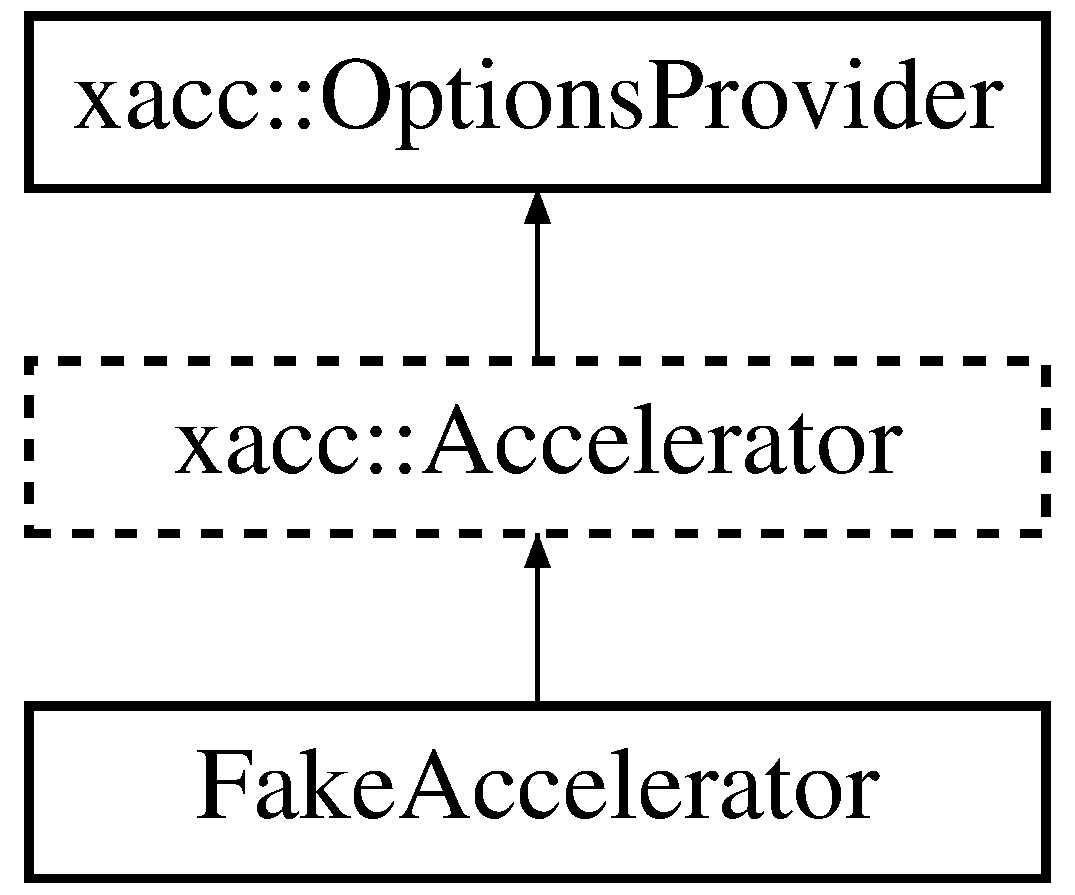
\includegraphics[height=3.000000cm]{a02496}
\end{center}
\end{figure}
\subsection*{Public Member Functions}
\begin{DoxyCompactItemize}
\item 
virtual Accelerator\+Type \hyperlink{a02496_abde88dbbf4410bf1c2c3826999e32d47}{get\+Type} ()
\item 
std\+::shared\+\_\+ptr$<$ \hyperlink{a02444}{Accelerator\+Buffer} $>$ \hyperlink{a02496_ae39580fdc83ce9f4df0967382398950e}{create\+Buffer} (const std\+::string \&var\+Id)
\item 
std\+::shared\+\_\+ptr$<$ \hyperlink{a02444}{Accelerator\+Buffer} $>$ \hyperlink{a02496_a09f29b893338dfb0a56dd183cf6949fe}{create\+Buffer} (const std\+::string \&var\+Id, const int size)
\item 
virtual bool \hyperlink{a02496_a7a6e63d282dc38fc53c3f3d46ca2ba9b}{is\+Valid\+Buffer\+Size} (const int N\+Bits)
\item 
virtual std\+::vector$<$ \hyperlink{a02484}{I\+R\+Transformation} $>$ \hyperlink{a02496_a6be5485b52606b4543d7e08eda4d6b69}{get\+I\+R\+Transformations} ()
\item 
virtual void \hyperlink{a02496_a22c71bda017235865f1b7d4cc5e911fa}{execute} (std\+::shared\+\_\+ptr$<$ \hyperlink{a02444}{Accelerator\+Buffer} $>$ buffer, const std\+::shared\+\_\+ptr$<$ \hyperlink{a02456}{Function} $>$ ir)
\end{DoxyCompactItemize}
\subsection*{Additional Inherited Members}


\subsection{Member Function Documentation}
\mbox{\Hypertarget{a02496_ae39580fdc83ce9f4df0967382398950e}\label{a02496_ae39580fdc83ce9f4df0967382398950e}} 
\index{Fake\+Accelerator@{Fake\+Accelerator}!create\+Buffer@{create\+Buffer}}
\index{create\+Buffer@{create\+Buffer}!Fake\+Accelerator@{Fake\+Accelerator}}
\subsubsection{\texorpdfstring{create\+Buffer()}{createBuffer()}\hspace{0.1cm}{\footnotesize\ttfamily [1/2]}}
{\footnotesize\ttfamily std\+::shared\+\_\+ptr$<$\hyperlink{a02444}{Accelerator\+Buffer}$>$ Fake\+Accelerator\+::create\+Buffer (\begin{DoxyParamCaption}\item[{const std\+::string \&}]{var\+Id }\end{DoxyParamCaption})\hspace{0.3cm}{\ttfamily [inline]}, {\ttfamily [virtual]}}

Create, store, and return an \hyperlink{a02444}{Accelerator\+Buffer} with the given variable id string. This string serves as a unique identifier for future lookups and reuse of the \hyperlink{a02444}{Accelerator\+Buffer}.


\begin{DoxyParams}{Parameters}
{\em var\+Id} & \\
\hline
\end{DoxyParams}
\begin{DoxyReturn}{Returns}

\end{DoxyReturn}


Implements \hyperlink{a02432_aab5046e8d83ab390302e0f49533e95fc}{xacc\+::\+Accelerator}.

\mbox{\Hypertarget{a02496_a09f29b893338dfb0a56dd183cf6949fe}\label{a02496_a09f29b893338dfb0a56dd183cf6949fe}} 
\index{Fake\+Accelerator@{Fake\+Accelerator}!create\+Buffer@{create\+Buffer}}
\index{create\+Buffer@{create\+Buffer}!Fake\+Accelerator@{Fake\+Accelerator}}
\subsubsection{\texorpdfstring{create\+Buffer()}{createBuffer()}\hspace{0.1cm}{\footnotesize\ttfamily [2/2]}}
{\footnotesize\ttfamily std\+::shared\+\_\+ptr$<$\hyperlink{a02444}{Accelerator\+Buffer}$>$ Fake\+Accelerator\+::create\+Buffer (\begin{DoxyParamCaption}\item[{const std\+::string \&}]{var\+Id,  }\item[{const int}]{size }\end{DoxyParamCaption})\hspace{0.3cm}{\ttfamily [inline]}, {\ttfamily [virtual]}}

Create, store, and return an \hyperlink{a02444}{Accelerator\+Buffer} with the given variable id string and of the given number of bits. The string id serves as a unique identifier for future lookups and reuse of the \hyperlink{a02444}{Accelerator\+Buffer}.


\begin{DoxyParams}{Parameters}
{\em var\+Id} & \\
\hline
{\em size} & \\
\hline
\end{DoxyParams}
\begin{DoxyReturn}{Returns}

\end{DoxyReturn}


Implements \hyperlink{a02432_a064a2dbd58338364115c260267806945}{xacc\+::\+Accelerator}.

\mbox{\Hypertarget{a02496_a22c71bda017235865f1b7d4cc5e911fa}\label{a02496_a22c71bda017235865f1b7d4cc5e911fa}} 
\index{Fake\+Accelerator@{Fake\+Accelerator}!execute@{execute}}
\index{execute@{execute}!Fake\+Accelerator@{Fake\+Accelerator}}
\subsubsection{\texorpdfstring{execute()}{execute()}}
{\footnotesize\ttfamily virtual void Fake\+Accelerator\+::execute (\begin{DoxyParamCaption}\item[{std\+::shared\+\_\+ptr$<$ \hyperlink{a02444}{Accelerator\+Buffer} $>$}]{buffer,  }\item[{const std\+::shared\+\_\+ptr$<$ \hyperlink{a02456}{Function} $>$}]{function }\end{DoxyParamCaption})\hspace{0.3cm}{\ttfamily [inline]}, {\ttfamily [virtual]}}

Execute the provided X\+A\+CC IR Function on the provided \hyperlink{a02444}{Accelerator\+Buffer}.


\begin{DoxyParams}{Parameters}
{\em buffer} & \\
\hline
{\em ir} & \\
\hline
\end{DoxyParams}


Implements \hyperlink{a02432_a89b3f3e6294f228abf03a410b0fb1674}{xacc\+::\+Accelerator}.

\mbox{\Hypertarget{a02496_a6be5485b52606b4543d7e08eda4d6b69}\label{a02496_a6be5485b52606b4543d7e08eda4d6b69}} 
\index{Fake\+Accelerator@{Fake\+Accelerator}!get\+I\+R\+Transformations@{get\+I\+R\+Transformations}}
\index{get\+I\+R\+Transformations@{get\+I\+R\+Transformations}!Fake\+Accelerator@{Fake\+Accelerator}}
\subsubsection{\texorpdfstring{get\+I\+R\+Transformations()}{getIRTransformations()}}
{\footnotesize\ttfamily virtual std\+::vector$<$\hyperlink{a02484}{I\+R\+Transformation}$>$ Fake\+Accelerator\+::get\+I\+R\+Transformations (\begin{DoxyParamCaption}{ }\end{DoxyParamCaption})\hspace{0.3cm}{\ttfamily [inline]}, {\ttfamily [virtual]}}

Return any IR Transformations that must be applied to ensure the compiled IR is amenable to execution on this Accelerator. \begin{DoxyReturn}{Returns}

\end{DoxyReturn}


Implements \hyperlink{a02432_ad6e4a642dcb24e552675bcbeff1e1b04}{xacc\+::\+Accelerator}.

\mbox{\Hypertarget{a02496_abde88dbbf4410bf1c2c3826999e32d47}\label{a02496_abde88dbbf4410bf1c2c3826999e32d47}} 
\index{Fake\+Accelerator@{Fake\+Accelerator}!get\+Type@{get\+Type}}
\index{get\+Type@{get\+Type}!Fake\+Accelerator@{Fake\+Accelerator}}
\subsubsection{\texorpdfstring{get\+Type()}{getType()}}
{\footnotesize\ttfamily virtual Accelerator\+Type Fake\+Accelerator\+::get\+Type (\begin{DoxyParamCaption}{ }\end{DoxyParamCaption})\hspace{0.3cm}{\ttfamily [inline]}, {\ttfamily [virtual]}}

Return the type of this Accelerator.

\begin{DoxyReturn}{Returns}
type The Accelerator type -\/ Gate or A\+QC Q\+PU, or N\+PU 
\end{DoxyReturn}


Implements \hyperlink{a02432_aaffc3e4bb9880eb5041b1b58ee4c2665}{xacc\+::\+Accelerator}.

\mbox{\Hypertarget{a02496_a7a6e63d282dc38fc53c3f3d46ca2ba9b}\label{a02496_a7a6e63d282dc38fc53c3f3d46ca2ba9b}} 
\index{Fake\+Accelerator@{Fake\+Accelerator}!is\+Valid\+Buffer\+Size@{is\+Valid\+Buffer\+Size}}
\index{is\+Valid\+Buffer\+Size@{is\+Valid\+Buffer\+Size}!Fake\+Accelerator@{Fake\+Accelerator}}
\subsubsection{\texorpdfstring{is\+Valid\+Buffer\+Size()}{isValidBufferSize()}}
{\footnotesize\ttfamily virtual bool Fake\+Accelerator\+::is\+Valid\+Buffer\+Size (\begin{DoxyParamCaption}\item[{const int}]{N\+Bits }\end{DoxyParamCaption})\hspace{0.3cm}{\ttfamily [inline]}, {\ttfamily [virtual]}}

Return true if this Accelerator can allocated N\+Bits number of bits. 
\begin{DoxyParams}{Parameters}
{\em N\+Bits} & \\
\hline
\end{DoxyParams}
\begin{DoxyReturn}{Returns}

\end{DoxyReturn}


Implements \hyperlink{a02432_ae51584850faeec77299058383977ddeb}{xacc\+::\+Accelerator}.



The documentation for this class was generated from the following file\+:\begin{DoxyCompactItemize}
\item 
Program\+Tester.\+cpp\end{DoxyCompactItemize}

\hypertarget{a01224}{}\section{Fake\+Http\+Client Class Reference}
\label{a01224}\index{Fake\+Http\+Client@{Fake\+Http\+Client}}
Inheritance diagram for Fake\+Http\+Client\+:\begin{figure}[H]
\begin{center}
\leavevmode
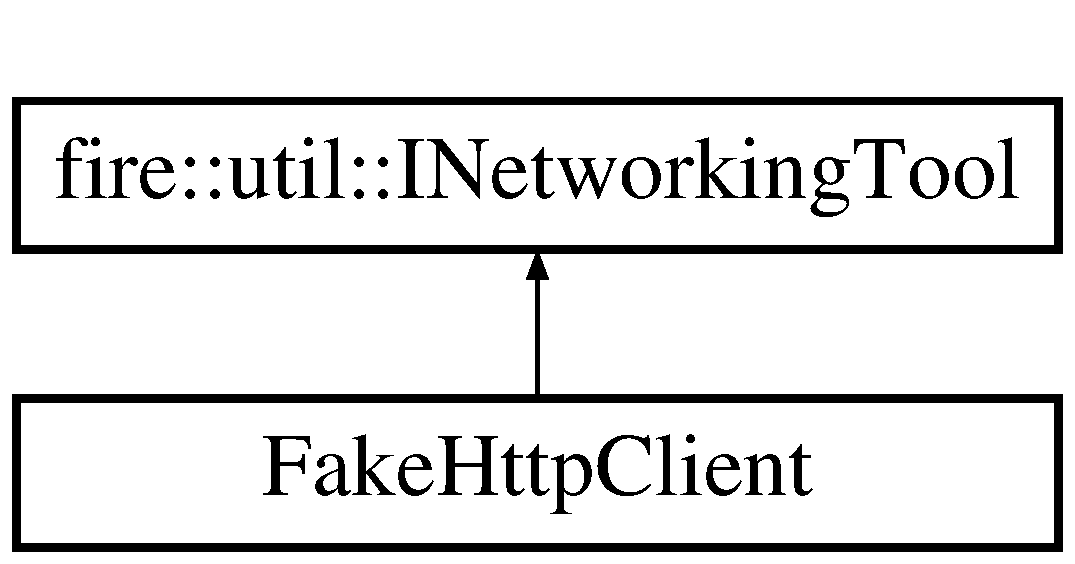
\includegraphics[height=2.000000cm]{a01224}
\end{center}
\end{figure}
\subsection*{Public Member Functions}
\begin{DoxyCompactItemize}
\item 
virtual std\+::string \hyperlink{a01224_a1bc1c2f1b3a0efb383aabb5a3a8080e6}{get} (const std\+::string \&relative\+Path, const std\+::map$<$ std\+::string, std\+::string $>$ \&header=std\+::map$<$ std\+::string, std\+::string $>$())
\item 
virtual \hyperlink{a01972}{fire\+::util\+::\+Post\+Response} \hyperlink{a01224_ae5364b5e675139717fca7b8add4226da}{post} (const std\+::string \&relative\+Path, const std\+::string \&message, const std\+::map$<$ std\+::string, std\+::string $>$ \&header=std\+::map$<$ std\+::string, std\+::string $>$())
\end{DoxyCompactItemize}
\subsection*{Public Attributes}
\begin{DoxyCompactItemize}
\item 
\mbox{\Hypertarget{a01224_aa4f56c4906c5c5654f05778b97860441}\label{a01224_aa4f56c4906c5c5654f05778b97860441}} 
bool {\bfseries post\+Occured} = false
\end{DoxyCompactItemize}
\subsection*{Additional Inherited Members}


\subsection{Member Function Documentation}
\mbox{\Hypertarget{a01224_a1bc1c2f1b3a0efb383aabb5a3a8080e6}\label{a01224_a1bc1c2f1b3a0efb383aabb5a3a8080e6}} 
\index{Fake\+Http\+Client@{Fake\+Http\+Client}!get@{get}}
\index{get@{get}!Fake\+Http\+Client@{Fake\+Http\+Client}}
\subsubsection{\texorpdfstring{get()}{get()}}
{\footnotesize\ttfamily virtual std\+::string Fake\+Http\+Client\+::get (\begin{DoxyParamCaption}\item[{const std\+::string \&}]{relative\+Path,  }\item[{const std\+::map$<$ std\+::string, std\+::string $>$ \&}]{header = {\ttfamily std\+:\+:map$<$~std\+:\+:string,~std\+:\+:string~$>$()} }\end{DoxyParamCaption})\hspace{0.3cm}{\ttfamily [inline]}, {\ttfamily [virtual]}}

Issue an H\+T\+TP G\+ET Command at the given relative path. Clients can provide a map of header key values to modify the G\+ET request.


\begin{DoxyParams}{Parameters}
{\em relative\+Path} & The path relative to the hostname/port provided to this Networking\+Tool \\
\hline
\end{DoxyParams}
\begin{DoxyReturn}{Returns}
The contents at the U\+RL or an error message if one took place. 
\end{DoxyReturn}


Implements \hyperlink{a01976_a58e9426e58cbb9c3b975b9d3e6c1f78f}{fire\+::util\+::\+I\+Networking\+Tool}.

\mbox{\Hypertarget{a01224_ae5364b5e675139717fca7b8add4226da}\label{a01224_ae5364b5e675139717fca7b8add4226da}} 
\index{Fake\+Http\+Client@{Fake\+Http\+Client}!post@{post}}
\index{post@{post}!Fake\+Http\+Client@{Fake\+Http\+Client}}
\subsubsection{\texorpdfstring{post()}{post()}}
{\footnotesize\ttfamily virtual \hyperlink{a01972}{fire\+::util\+::\+Post\+Response} Fake\+Http\+Client\+::post (\begin{DoxyParamCaption}\item[{const std\+::string \&}]{relative\+Path,  }\item[{const std\+::string \&}]{message,  }\item[{const std\+::map$<$ std\+::string, std\+::string $>$ \&}]{header = {\ttfamily std\+:\+:map$<$~std\+:\+:string,~std\+:\+:string$>$()} }\end{DoxyParamCaption})\hspace{0.3cm}{\ttfamily [inline]}, {\ttfamily [virtual]}}

Issue an H\+T\+TP Post command at the given relative path with the provided message. Clients can provide a map of header key values to modify the P\+O\+ST request.


\begin{DoxyParams}{Parameters}
{\em relative\+Path} & The path relative to the hostname/port provided to this Networking\+Tool \\
\hline
{\em message} & The message to post \\
\hline
{\em header} & The map of additional H\+T\+TP P\+O\+ST header information \\
\hline
\end{DoxyParams}
\begin{DoxyReturn}{Returns}
success Boolean indicating if post was successful 
\end{DoxyReturn}


Implements \hyperlink{a01976_aa585d9b27c43f698203e6c6ec1ee05ce}{fire\+::util\+::\+I\+Networking\+Tool}.



The documentation for this class was generated from the following file\+:\begin{DoxyCompactItemize}
\item 
Rigetti\+Accelerator\+Tester.\+cpp\end{DoxyCompactItemize}

\hypertarget{a02492}{}\section{Fake\+IR Class Reference}
\label{a02492}\index{Fake\+IR@{Fake\+IR}}
Inheritance diagram for Fake\+IR\+:\begin{figure}[H]
\begin{center}
\leavevmode
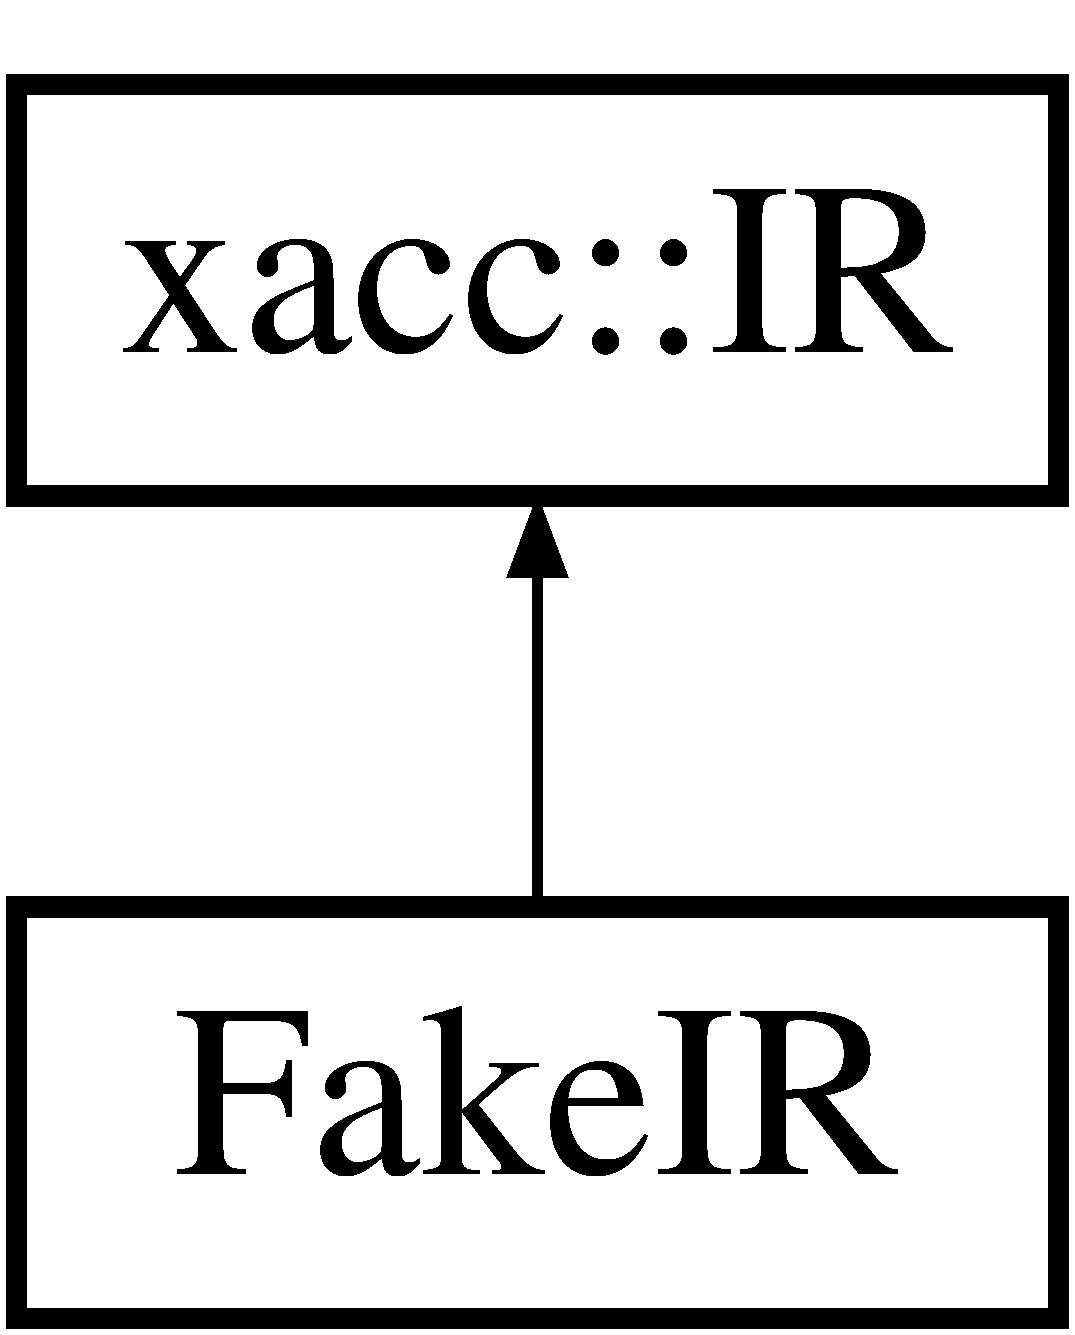
\includegraphics[height=2.000000cm]{a02492}
\end{center}
\end{figure}
\subsection*{Public Member Functions}
\begin{DoxyCompactItemize}
\item 
virtual std\+::string \hyperlink{a02492_ac8b4fa63654de7830e2a6110559ffd87}{to\+Assembly\+String} (const std\+::string \&kernel\+Name, const std\+::string \&acc\+Buffer\+Var\+Name)
\item 
virtual void \hyperlink{a02492_a459bd7e4a007ab80678df279eb038b51}{persist} (std\+::ostream \&stream)
\item 
virtual void \hyperlink{a02492_ad079b5e83c97bc7fae776679e0f93a1e}{load} (std\+::istream \&in\+Stream)
\item 
virtual void \hyperlink{a02492_a526ef10e1ee21f5552b1ca61872f541a}{add\+Kernel} (std\+::shared\+\_\+ptr$<$ \hyperlink{a02456}{Function} $>$ kernel)
\item 
virtual std\+::shared\+\_\+ptr$<$ \hyperlink{a02456}{Function} $>$ \hyperlink{a02492_a351b9a1f9fb748612f5a39007c421efc}{get\+Kernel} (const std\+::string \&name)
\end{DoxyCompactItemize}


\subsection{Member Function Documentation}
\mbox{\Hypertarget{a02492_a526ef10e1ee21f5552b1ca61872f541a}\label{a02492_a526ef10e1ee21f5552b1ca61872f541a}} 
\index{Fake\+IR@{Fake\+IR}!add\+Kernel@{add\+Kernel}}
\index{add\+Kernel@{add\+Kernel}!Fake\+IR@{Fake\+IR}}
\subsubsection{\texorpdfstring{add\+Kernel()}{addKernel()}}
{\footnotesize\ttfamily virtual void Fake\+I\+R\+::add\+Kernel (\begin{DoxyParamCaption}\item[{std\+::shared\+\_\+ptr$<$ \hyperlink{a02456}{Function} $>$}]{kernel }\end{DoxyParamCaption})\hspace{0.3cm}{\ttfamily [inline]}, {\ttfamily [virtual]}}

Add a new kernel to this IR instance.


\begin{DoxyParams}{Parameters}
{\em kernel} & The Function instance to add as a new kernel \\
\hline
\end{DoxyParams}


Implements \hyperlink{a02480_abbbf8e6993c518597de32cd05d49d737}{xacc\+::\+IR}.

\mbox{\Hypertarget{a02492_a351b9a1f9fb748612f5a39007c421efc}\label{a02492_a351b9a1f9fb748612f5a39007c421efc}} 
\index{Fake\+IR@{Fake\+IR}!get\+Kernel@{get\+Kernel}}
\index{get\+Kernel@{get\+Kernel}!Fake\+IR@{Fake\+IR}}
\subsubsection{\texorpdfstring{get\+Kernel()}{getKernel()}}
{\footnotesize\ttfamily virtual std\+::shared\+\_\+ptr$<$\hyperlink{a02456}{Function}$>$ Fake\+I\+R\+::get\+Kernel (\begin{DoxyParamCaption}\item[{const std\+::string \&}]{name }\end{DoxyParamCaption})\hspace{0.3cm}{\ttfamily [inline]}, {\ttfamily [virtual]}}

Return the kernel with the given name.


\begin{DoxyParams}{Parameters}
{\em name} & The name of the kernel to return. \\
\hline
\end{DoxyParams}
\begin{DoxyReturn}{Returns}
kernel The kernel with given name. 
\end{DoxyReturn}


Implements \hyperlink{a02480_a6f49b4ba4b3a15142b04873284885f0d}{xacc\+::\+IR}.

\mbox{\Hypertarget{a02492_ad079b5e83c97bc7fae776679e0f93a1e}\label{a02492_ad079b5e83c97bc7fae776679e0f93a1e}} 
\index{Fake\+IR@{Fake\+IR}!load@{load}}
\index{load@{load}!Fake\+IR@{Fake\+IR}}
\subsubsection{\texorpdfstring{load()}{load()}}
{\footnotesize\ttfamily virtual void Fake\+I\+R\+::load (\begin{DoxyParamCaption}\item[{std\+::istream \&}]{in\+Stream }\end{DoxyParamCaption})\hspace{0.3cm}{\ttfamily [inline]}, {\ttfamily [virtual]}}

Create this IR instance from the given input stream.


\begin{DoxyParams}{Parameters}
{\em in\+Stream} & The input stream to read from. \\
\hline
\end{DoxyParams}


Implements \hyperlink{a02480_a444c2e4dc0faac500fb70fa93997e9bc}{xacc\+::\+IR}.

\mbox{\Hypertarget{a02492_a459bd7e4a007ab80678df279eb038b51}\label{a02492_a459bd7e4a007ab80678df279eb038b51}} 
\index{Fake\+IR@{Fake\+IR}!persist@{persist}}
\index{persist@{persist}!Fake\+IR@{Fake\+IR}}
\subsubsection{\texorpdfstring{persist()}{persist()}}
{\footnotesize\ttfamily virtual void Fake\+I\+R\+::persist (\begin{DoxyParamCaption}\item[{std\+::ostream \&}]{out\+Stream }\end{DoxyParamCaption})\hspace{0.3cm}{\ttfamily [inline]}, {\ttfamily [virtual]}}

Persist this IR instance to the given output stream.


\begin{DoxyParams}{Parameters}
{\em out\+Stream} & The output stream to persist to. \\
\hline
\end{DoxyParams}


Implements \hyperlink{a02480_a414b72224d88473ad6190bb88102a3ea}{xacc\+::\+IR}.

\mbox{\Hypertarget{a02492_ac8b4fa63654de7830e2a6110559ffd87}\label{a02492_ac8b4fa63654de7830e2a6110559ffd87}} 
\index{Fake\+IR@{Fake\+IR}!to\+Assembly\+String@{to\+Assembly\+String}}
\index{to\+Assembly\+String@{to\+Assembly\+String}!Fake\+IR@{Fake\+IR}}
\subsubsection{\texorpdfstring{to\+Assembly\+String()}{toAssemblyString()}}
{\footnotesize\ttfamily virtual std\+::string Fake\+I\+R\+::to\+Assembly\+String (\begin{DoxyParamCaption}\item[{const std\+::string \&}]{kernel\+Name,  }\item[{const std\+::string \&}]{acc\+Buffer\+Var\+Name }\end{DoxyParamCaption})\hspace{0.3cm}{\ttfamily [inline]}, {\ttfamily [virtual]}}

Return a assembly-\/like string representation of this intermediate representation


\begin{DoxyParams}{Parameters}
{\em kernel\+Name} & The name of hte kernel to persist to string \\
\hline
{\em acc\+Buffer\+Var\+Name} & The name of the \hyperlink{a02444}{Accelerator\+Buffer} \\
\hline
\end{DoxyParams}
\begin{DoxyReturn}{Returns}

\end{DoxyReturn}


Implements \hyperlink{a02480_a8356cdff1919b88eabeb84fd7450cdb6}{xacc\+::\+IR}.



The documentation for this class was generated from the following file\+:\begin{DoxyCompactItemize}
\item 
Program\+Tester.\+cpp\end{DoxyCompactItemize}

\hypertarget{a01784}{}\section{File\+Generator Struct Reference}
\label{a01784}\index{File\+Generator@{File\+Generator}}


The documentation for this struct was generated from the following file\+:\begin{DoxyCompactItemize}
\item 
Delimited\+Text\+Parser\+Test.\+cpp\end{DoxyCompactItemize}

\hypertarget{a02192}{}\section{File\+Read\+Stream Class Reference}
\label{a02192}\index{File\+Read\+Stream@{File\+Read\+Stream}}


File byte stream for input using fread().  




{\ttfamily \#include $<$filereadstream.\+h$>$}

\subsection*{Public Types}
\begin{DoxyCompactItemize}
\item 
\mbox{\Hypertarget{a02192_ae1f83d9ca3c76d1d151af0b6c427f046}\label{a02192_ae1f83d9ca3c76d1d151af0b6c427f046}} 
typedef char \hyperlink{a02192_ae1f83d9ca3c76d1d151af0b6c427f046}{Ch}
\begin{DoxyCompactList}\small\item\em Character type (byte). \end{DoxyCompactList}\end{DoxyCompactItemize}
\subsection*{Public Member Functions}
\begin{DoxyCompactItemize}
\item 
\hyperlink{a02192_adf91191843d50b900f43cb4f35f16f67}{File\+Read\+Stream} (std\+::\+F\+I\+LE $\ast$fp, char $\ast$buffer, size\+\_\+t buffer\+Size)
\begin{DoxyCompactList}\small\item\em Constructor. \end{DoxyCompactList}\item 
\mbox{\Hypertarget{a02192_ab7d47da8952d3fe5856a261ec3c020c9}\label{a02192_ab7d47da8952d3fe5856a261ec3c020c9}} 
\hyperlink{a02192_ae1f83d9ca3c76d1d151af0b6c427f046}{Ch} {\bfseries Peek} () const
\item 
\mbox{\Hypertarget{a02192_addcbccc9d86ccbbe6d8e876ba595dbcb}\label{a02192_addcbccc9d86ccbbe6d8e876ba595dbcb}} 
\hyperlink{a02192_ae1f83d9ca3c76d1d151af0b6c427f046}{Ch} {\bfseries Take} ()
\item 
\mbox{\Hypertarget{a02192_ae82cfaafe347286b3af8976548bedf86}\label{a02192_ae82cfaafe347286b3af8976548bedf86}} 
size\+\_\+t {\bfseries Tell} () const
\item 
\mbox{\Hypertarget{a02192_a4f2eac5b08033b1527bff517be657a36}\label{a02192_a4f2eac5b08033b1527bff517be657a36}} 
void {\bfseries Put} (\hyperlink{a02192_ae1f83d9ca3c76d1d151af0b6c427f046}{Ch})
\item 
\mbox{\Hypertarget{a02192_acd031e3f578b23bc2a792ac41e1e95ae}\label{a02192_acd031e3f578b23bc2a792ac41e1e95ae}} 
void {\bfseries Flush} ()
\item 
\mbox{\Hypertarget{a02192_ac985850ab75f204dc08a01d12a8ef5c6}\label{a02192_ac985850ab75f204dc08a01d12a8ef5c6}} 
\hyperlink{a02192_ae1f83d9ca3c76d1d151af0b6c427f046}{Ch} $\ast$ {\bfseries Put\+Begin} ()
\item 
\mbox{\Hypertarget{a02192_a886660c89f698ff913d641d61466108f}\label{a02192_a886660c89f698ff913d641d61466108f}} 
size\+\_\+t {\bfseries Put\+End} (\hyperlink{a02192_ae1f83d9ca3c76d1d151af0b6c427f046}{Ch} $\ast$)
\item 
\mbox{\Hypertarget{a02192_a03f0b804c4c96762d0c6ef536337b7f0}\label{a02192_a03f0b804c4c96762d0c6ef536337b7f0}} 
const \hyperlink{a02192_ae1f83d9ca3c76d1d151af0b6c427f046}{Ch} $\ast$ {\bfseries Peek4} () const
\end{DoxyCompactItemize}


\subsection{Detailed Description}
File byte stream for input using fread(). 

\begin{DoxyNote}{Note}
implements Stream concept 
\end{DoxyNote}


\subsection{Constructor \& Destructor Documentation}
\mbox{\Hypertarget{a02192_adf91191843d50b900f43cb4f35f16f67}\label{a02192_adf91191843d50b900f43cb4f35f16f67}} 
\index{File\+Read\+Stream@{File\+Read\+Stream}!File\+Read\+Stream@{File\+Read\+Stream}}
\index{File\+Read\+Stream@{File\+Read\+Stream}!File\+Read\+Stream@{File\+Read\+Stream}}
\subsubsection{\texorpdfstring{File\+Read\+Stream()}{FileReadStream()}}
{\footnotesize\ttfamily File\+Read\+Stream\+::\+File\+Read\+Stream (\begin{DoxyParamCaption}\item[{std\+::\+F\+I\+LE $\ast$}]{fp,  }\item[{char $\ast$}]{buffer,  }\item[{size\+\_\+t}]{buffer\+Size }\end{DoxyParamCaption})\hspace{0.3cm}{\ttfamily [inline]}}



Constructor. 


\begin{DoxyParams}{Parameters}
{\em fp} & File pointer opened for read. \\
\hline
{\em buffer} & user-\/supplied buffer. \\
\hline
{\em buffer\+Size} & size of buffer in bytes. Must $>$=4 bytes. \\
\hline
\end{DoxyParams}


The documentation for this class was generated from the following file\+:\begin{DoxyCompactItemize}
\item 
filereadstream.\+h\end{DoxyCompactItemize}

\hypertarget{a01868}{}\section{C\+Simple\+Ini\+Templ$<$ S\+I\+\_\+\+C\+H\+AR, S\+I\+\_\+\+S\+T\+R\+L\+E\+SS, S\+I\+\_\+\+C\+O\+N\+V\+E\+R\+T\+ER $>$\+:\+:File\+Writer Class Reference}
\label{a01868}\index{C\+Simple\+Ini\+Templ$<$ S\+I\+\_\+\+C\+H\+A\+R, S\+I\+\_\+\+S\+T\+R\+L\+E\+S\+S, S\+I\+\_\+\+C\+O\+N\+V\+E\+R\+T\+E\+R $>$\+::\+File\+Writer@{C\+Simple\+Ini\+Templ$<$ S\+I\+\_\+\+C\+H\+A\+R, S\+I\+\_\+\+S\+T\+R\+L\+E\+S\+S, S\+I\+\_\+\+C\+O\+N\+V\+E\+R\+T\+E\+R $>$\+::\+File\+Writer}}


{\ttfamily \#include $<$Simple\+Ini.\+h$>$}

Inheritance diagram for C\+Simple\+Ini\+Templ$<$ S\+I\+\_\+\+C\+H\+AR, S\+I\+\_\+\+S\+T\+R\+L\+E\+SS, S\+I\+\_\+\+C\+O\+N\+V\+E\+R\+T\+ER $>$\+:\+:File\+Writer\+:\begin{figure}[H]
\begin{center}
\leavevmode
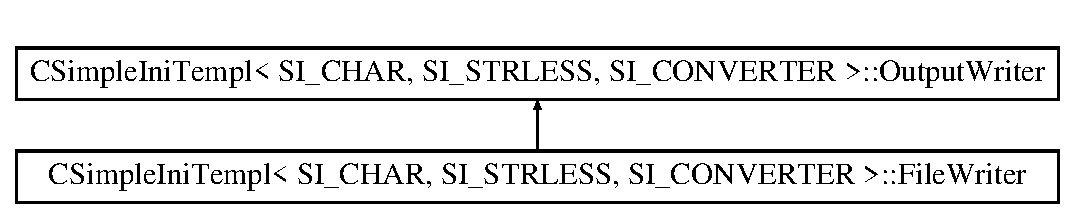
\includegraphics[height=2.000000cm]{a01868}
\end{center}
\end{figure}
\subsection*{Public Member Functions}
\begin{DoxyCompactItemize}
\item 
\mbox{\Hypertarget{a01868_aecd4d79480c9b4e70b598c10014856f8}\label{a01868_aecd4d79480c9b4e70b598c10014856f8}} 
{\bfseries File\+Writer} (F\+I\+LE $\ast$a\+\_\+file)
\item 
\mbox{\Hypertarget{a01868_ae8885b97884ef9dd5bf074bc4f011373}\label{a01868_ae8885b97884ef9dd5bf074bc4f011373}} 
void {\bfseries Write} (const char $\ast$a\+\_\+p\+Buf)
\end{DoxyCompactItemize}


\subsection{Detailed Description}
\subsubsection*{template$<$class S\+I\+\_\+\+C\+H\+AR, class S\+I\+\_\+\+S\+T\+R\+L\+E\+SS, class S\+I\+\_\+\+C\+O\+N\+V\+E\+R\+T\+ER$>$\newline
class C\+Simple\+Ini\+Templ$<$ S\+I\+\_\+\+C\+H\+A\+R, S\+I\+\_\+\+S\+T\+R\+L\+E\+S\+S, S\+I\+\_\+\+C\+O\+N\+V\+E\+R\+T\+E\+R $>$\+::\+File\+Writer}

\hyperlink{a01864}{Output\+Writer} class to write the I\+NI data to a file 

The documentation for this class was generated from the following file\+:\begin{DoxyCompactItemize}
\item 
Simple\+Ini.\+h\end{DoxyCompactItemize}

\hypertarget{a02196}{}\section{File\+Write\+Stream Class Reference}
\label{a02196}\index{File\+Write\+Stream@{File\+Write\+Stream}}


Wrapper of C file stream for input using fread().  




{\ttfamily \#include $<$filewritestream.\+h$>$}

\subsection*{Public Types}
\begin{DoxyCompactItemize}
\item 
\mbox{\Hypertarget{a02196_abc16aeb69ad4176263ddfcb837fb7b49}\label{a02196_abc16aeb69ad4176263ddfcb837fb7b49}} 
typedef char \hyperlink{a02196_abc16aeb69ad4176263ddfcb837fb7b49}{Ch}
\begin{DoxyCompactList}\small\item\em Character type. Only support char. \end{DoxyCompactList}\end{DoxyCompactItemize}
\subsection*{Public Member Functions}
\begin{DoxyCompactItemize}
\item 
\mbox{\Hypertarget{a02196_a553ea3e7377a7f7cace2daa3cc90e1a1}\label{a02196_a553ea3e7377a7f7cace2daa3cc90e1a1}} 
{\bfseries File\+Write\+Stream} (std\+::\+F\+I\+LE $\ast$fp, char $\ast$buffer, size\+\_\+t buffer\+Size)
\item 
\mbox{\Hypertarget{a02196_af6a6061d0accd939fa475b9b34427d85}\label{a02196_af6a6061d0accd939fa475b9b34427d85}} 
void {\bfseries Put} (char c)
\item 
\mbox{\Hypertarget{a02196_ad9ec108b24316a2c1c83c6ddc75d308a}\label{a02196_ad9ec108b24316a2c1c83c6ddc75d308a}} 
void {\bfseries PutN} (char c, size\+\_\+t n)
\item 
\mbox{\Hypertarget{a02196_a939fbf183ba36464c5e0837df4329d37}\label{a02196_a939fbf183ba36464c5e0837df4329d37}} 
void {\bfseries Flush} ()
\item 
\mbox{\Hypertarget{a02196_ab556c7e26346ddff0e579a53c09c3a13}\label{a02196_ab556c7e26346ddff0e579a53c09c3a13}} 
char {\bfseries Peek} () const
\item 
\mbox{\Hypertarget{a02196_ac927a0ae09a85eaba58a74ceb04b40ed}\label{a02196_ac927a0ae09a85eaba58a74ceb04b40ed}} 
char {\bfseries Take} ()
\item 
\mbox{\Hypertarget{a02196_a06272de32d6ac4d10c9bd5deb79a0234}\label{a02196_a06272de32d6ac4d10c9bd5deb79a0234}} 
size\+\_\+t {\bfseries Tell} () const
\item 
\mbox{\Hypertarget{a02196_a4d1340a64fde3f16ac2afce19537c75e}\label{a02196_a4d1340a64fde3f16ac2afce19537c75e}} 
char $\ast$ {\bfseries Put\+Begin} ()
\item 
\mbox{\Hypertarget{a02196_a54b14047e4c998db0594290605f8f0dc}\label{a02196_a54b14047e4c998db0594290605f8f0dc}} 
size\+\_\+t {\bfseries Put\+End} (char $\ast$)
\end{DoxyCompactItemize}


\subsection{Detailed Description}
Wrapper of C file stream for input using fread(). 

\begin{DoxyNote}{Note}
implements Stream concept 
\end{DoxyNote}


The documentation for this class was generated from the following file\+:\begin{DoxyCompactItemize}
\item 
filewritestream.\+h\end{DoxyCompactItemize}

\hypertarget{a02084}{}\section{Generic\+Value$<$ Encoding, Allocator $>$\+:\+:Flag Struct Reference}
\label{a02084}\index{Generic\+Value$<$ Encoding, Allocator $>$\+::\+Flag@{Generic\+Value$<$ Encoding, Allocator $>$\+::\+Flag}}
\subsection*{Public Attributes}
\begin{DoxyCompactItemize}
\item 
\mbox{\Hypertarget{a02084_aced7ede2056a797fb80817d45634e3ea}\label{a02084_aced7ede2056a797fb80817d45634e3ea}} 
char {\bfseries payload} \mbox{[}sizeof(\hyperlink{a00560_a5ed6e6e67250fadbd041127e6386dcb5}{Size\+Type}) $\ast$2+sizeof(void $\ast$)+2\mbox{]}
\item 
\mbox{\Hypertarget{a02084_ac91f08067dcc0003fc78e870ca9b2d5d}\label{a02084_ac91f08067dcc0003fc78e870ca9b2d5d}} 
uint16\+\_\+t {\bfseries flags}
\end{DoxyCompactItemize}


The documentation for this struct was generated from the following file\+:\begin{DoxyCompactItemize}
\item 
\hyperlink{a00476}{document.\+h}\end{DoxyCompactItemize}

\hypertarget{a01792}{}\section{foo Class Reference}
\label{a01792}\index{foo@{foo}}


{\ttfamily \#include $<$O\+D\+E\+Solver.\+h$>$}



\subsection{Detailed Description}


 Copyright (c) 2015-\/, U\+T-\/\+Battelle, L\+LC All rights reserved.

Redistribution and use in source and binary forms, with or without modification, are permitted provided that the following conditions are met\+:

Redistributions of source code must retain the above copyright notice, this list of conditions and the following disclaimer.

Redistributions in binary form must reproduce the above copyright notice, this list of conditions and the following disclaimer in the documentation and/or other materials provided with the distribution.

Neither the name of fern nor the names of its contributors may be used to endorse or promote products derived from this software without specific prior written permission.

T\+H\+IS S\+O\+F\+T\+W\+A\+RE IS P\+R\+O\+V\+I\+D\+ED BY T\+HE C\+O\+P\+Y\+R\+I\+G\+HT H\+O\+L\+D\+E\+RS A\+ND C\+O\+N\+T\+R\+I\+B\+U\+T\+O\+RS \char`\"{}\+A\+S I\+S\char`\"{} A\+ND A\+NY E\+X\+P\+R\+E\+SS OR I\+M\+P\+L\+I\+ED W\+A\+R\+R\+A\+N\+T\+I\+ES, I\+N\+C\+L\+U\+D\+I\+NG, B\+UT N\+OT L\+I\+M\+I\+T\+ED TO, T\+HE I\+M\+P\+L\+I\+ED W\+A\+R\+R\+A\+N\+T\+I\+ES OF M\+E\+R\+C\+H\+A\+N\+T\+A\+B\+I\+L\+I\+TY A\+ND F\+I\+T\+N\+E\+SS F\+OR A P\+A\+R\+T\+I\+C\+U\+L\+AR P\+U\+R\+P\+O\+SE A\+RE D\+I\+S\+C\+L\+A\+I\+M\+ED. IN NO E\+V\+E\+NT S\+H\+A\+LL T\+HE C\+O\+P\+Y\+R\+I\+G\+HT H\+O\+L\+D\+ER OR C\+O\+N\+T\+R\+I\+B\+U\+T\+O\+RS BE L\+I\+A\+B\+LE F\+OR A\+NY D\+I\+R\+E\+CT, I\+N\+D\+I\+R\+E\+CT, I\+N\+C\+I\+D\+E\+N\+T\+AL, S\+P\+E\+C\+I\+AL, E\+X\+E\+M\+P\+L\+A\+RY, OR C\+O\+N\+S\+E\+Q\+U\+E\+N\+T\+I\+AL D\+A\+M\+A\+G\+ES (I\+N\+C\+L\+U\+D\+I\+NG, B\+UT N\+OT L\+I\+M\+I\+T\+ED TO, P\+R\+O\+C\+U\+R\+E\+M\+E\+NT OF S\+U\+B\+S\+T\+I\+T\+U\+TE G\+O\+O\+DS OR S\+E\+R\+V\+I\+C\+ES; L\+O\+SS OF U\+SE, D\+A\+TA, OR P\+R\+O\+F\+I\+TS; OR B\+U\+S\+I\+N\+E\+SS I\+N\+T\+E\+R\+R\+U\+P\+T\+I\+ON) H\+O\+W\+E\+V\+ER C\+A\+U\+S\+ED A\+ND ON A\+NY T\+H\+E\+O\+RY OF L\+I\+A\+B\+I\+L\+I\+TY, W\+H\+E\+T\+H\+ER IN C\+O\+N\+T\+R\+A\+CT, S\+T\+R\+I\+CT L\+I\+A\+B\+I\+L\+I\+TY, OR T\+O\+RT (I\+N\+C\+L\+U\+D\+I\+NG N\+E\+G\+L\+I\+G\+E\+N\+CE OR O\+T\+H\+E\+R\+W\+I\+SE) A\+R\+I\+S\+I\+NG IN A\+NY W\+AY O\+UT OF T\+HE U\+SE OF T\+H\+IS S\+O\+F\+T\+W\+A\+RE, E\+V\+EN IF A\+D\+V\+I\+S\+ED OF T\+HE P\+O\+S\+S\+I\+B\+I\+L\+I\+TY OF S\+U\+CH D\+A\+M\+A\+GE.

\subsubsection*{Author(s)\+: Jay Jay Billings (jayjaybillings  gmail  com) }

The documentation for this class was generated from the following file\+:\begin{DoxyCompactItemize}
\item 
O\+D\+E\+Solver.\+h\end{DoxyCompactItemize}

\hypertarget{a02456}{}\section{xacc\+:\+:Function Class Reference}
\label{a02456}\index{xacc\+::\+Function@{xacc\+::\+Function}}


{\ttfamily \#include $<$Function.\+hpp$>$}

Inheritance diagram for xacc\+:\+:Function\+:\begin{figure}[H]
\begin{center}
\leavevmode
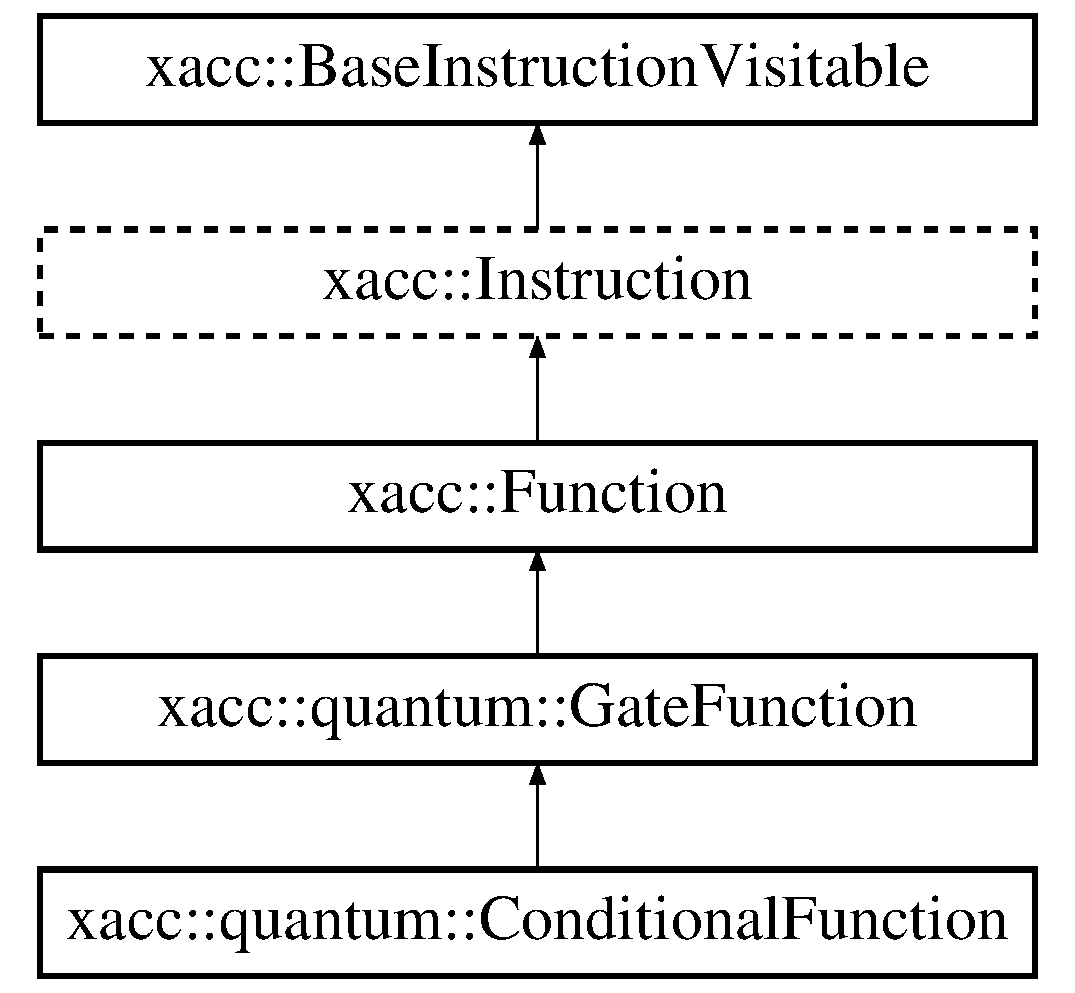
\includegraphics[height=5.000000cm]{a02456}
\end{center}
\end{figure}
\subsection*{Public Member Functions}
\begin{DoxyCompactItemize}
\item 
virtual const int \hyperlink{a02456_a8901985525f59713e14c61713e07c086}{n\+Instructions} ()=0
\item 
virtual Inst\+Ptr \hyperlink{a02456_afa549fc91b5a05f26d8139954a7e0ed5}{get\+Instruction} (const int idx)=0
\item 
virtual std\+::list$<$ Inst\+Ptr $>$ \hyperlink{a02456_aaf80bd3d49113a92b520785572663032}{get\+Instructions} ()=0
\item 
virtual void \hyperlink{a02456_ab6478b09bb28e194bb555b3180737733}{remove\+Instruction} (const int idx)=0
\item 
virtual void \hyperlink{a02456_a2ef6a4923a6734f90f6ee3d94d263af0}{replace\+Instruction} (const int idx, Inst\+Ptr new\+Inst)=0
\item 
virtual void \hyperlink{a02456_aa8c9ec2d08be75c69399d4254b0216f5}{add\+Instruction} (Inst\+Ptr instruction)=0
\item 
virtual bool \hyperlink{a02456_aa75500c657b5c3e0e36213e1506aad97}{is\+Composite} ()
\item 
virtual \hyperlink{a02456_a04b25ba4da1ddfa4ec4ec6d6ffb25bc3}{$\sim$\+Function} ()
\end{DoxyCompactItemize}
\subsection*{Additional Inherited Members}


\subsection{Detailed Description}
The \hyperlink{a02456}{Function} is an \hyperlink{a02460}{Instruction} that contains further child Instructions. 

\subsection{Constructor \& Destructor Documentation}
\mbox{\Hypertarget{a02456_a04b25ba4da1ddfa4ec4ec6d6ffb25bc3}\label{a02456_a04b25ba4da1ddfa4ec4ec6d6ffb25bc3}} 
\index{xacc\+::\+Function@{xacc\+::\+Function}!````~Function@{$\sim$\+Function}}
\index{````~Function@{$\sim$\+Function}!xacc\+::\+Function@{xacc\+::\+Function}}
\subsubsection{\texorpdfstring{$\sim$\+Function()}{~Function()}}
{\footnotesize\ttfamily virtual xacc\+::\+Function\+::$\sim$\+Function (\begin{DoxyParamCaption}{ }\end{DoxyParamCaption})\hspace{0.3cm}{\ttfamily [inline]}, {\ttfamily [virtual]}}

The destructor 

\subsection{Member Function Documentation}
\mbox{\Hypertarget{a02456_aa8c9ec2d08be75c69399d4254b0216f5}\label{a02456_aa8c9ec2d08be75c69399d4254b0216f5}} 
\index{xacc\+::\+Function@{xacc\+::\+Function}!add\+Instruction@{add\+Instruction}}
\index{add\+Instruction@{add\+Instruction}!xacc\+::\+Function@{xacc\+::\+Function}}
\subsubsection{\texorpdfstring{add\+Instruction()}{addInstruction()}}
{\footnotesize\ttfamily virtual void xacc\+::\+Function\+::add\+Instruction (\begin{DoxyParamCaption}\item[{Inst\+Ptr}]{instruction }\end{DoxyParamCaption})\hspace{0.3cm}{\ttfamily [pure virtual]}}

Add an \hyperlink{a02460}{Instruction} to this \hyperlink{a02456}{Function}.


\begin{DoxyParams}{Parameters}
{\em instruction} & The instruction to add. \\
\hline
\end{DoxyParams}


Implemented in \hyperlink{a01272_a892fb69a10f0a7cb5abdab4cca61b80a}{xacc\+::quantum\+::\+Gate\+Function}, and \hyperlink{a01304_a6aedad20f96390880efdc0a476b3273f}{xacc\+::quantum\+::\+Conditional\+Function}.

\mbox{\Hypertarget{a02456_afa549fc91b5a05f26d8139954a7e0ed5}\label{a02456_afa549fc91b5a05f26d8139954a7e0ed5}} 
\index{xacc\+::\+Function@{xacc\+::\+Function}!get\+Instruction@{get\+Instruction}}
\index{get\+Instruction@{get\+Instruction}!xacc\+::\+Function@{xacc\+::\+Function}}
\subsubsection{\texorpdfstring{get\+Instruction()}{getInstruction()}}
{\footnotesize\ttfamily virtual Inst\+Ptr xacc\+::\+Function\+::get\+Instruction (\begin{DoxyParamCaption}\item[{const int}]{idx }\end{DoxyParamCaption})\hspace{0.3cm}{\ttfamily [pure virtual]}}

Return the \hyperlink{a02460}{Instruction} at the given index.


\begin{DoxyParams}{Parameters}
{\em idx} & The desired \hyperlink{a02460}{Instruction} index \\
\hline
\end{DoxyParams}
\begin{DoxyReturn}{Returns}
inst The instruction at the given index. 
\end{DoxyReturn}


Implemented in \hyperlink{a01272_a841d656eed8aa9b4c0eec3f1da38069c}{xacc\+::quantum\+::\+Gate\+Function}.

\mbox{\Hypertarget{a02456_aaf80bd3d49113a92b520785572663032}\label{a02456_aaf80bd3d49113a92b520785572663032}} 
\index{xacc\+::\+Function@{xacc\+::\+Function}!get\+Instructions@{get\+Instructions}}
\index{get\+Instructions@{get\+Instructions}!xacc\+::\+Function@{xacc\+::\+Function}}
\subsubsection{\texorpdfstring{get\+Instructions()}{getInstructions()}}
{\footnotesize\ttfamily virtual std\+::list$<$Inst\+Ptr$>$ xacc\+::\+Function\+::get\+Instructions (\begin{DoxyParamCaption}{ }\end{DoxyParamCaption})\hspace{0.3cm}{\ttfamily [pure virtual]}}

Return all Instructions in this \hyperlink{a02456}{Function}

\begin{DoxyReturn}{Returns}
insts The list of this \hyperlink{a02456}{Function}\textquotesingle{}s Instructions 
\end{DoxyReturn}


Implemented in \hyperlink{a01272_aebce6a9e64aed7f4aff86df752bacfe2}{xacc\+::quantum\+::\+Gate\+Function}.

\mbox{\Hypertarget{a02456_aa75500c657b5c3e0e36213e1506aad97}\label{a02456_aa75500c657b5c3e0e36213e1506aad97}} 
\index{xacc\+::\+Function@{xacc\+::\+Function}!is\+Composite@{is\+Composite}}
\index{is\+Composite@{is\+Composite}!xacc\+::\+Function@{xacc\+::\+Function}}
\subsubsection{\texorpdfstring{is\+Composite()}{isComposite()}}
{\footnotesize\ttfamily virtual bool xacc\+::\+Function\+::is\+Composite (\begin{DoxyParamCaption}{ }\end{DoxyParamCaption})\hspace{0.3cm}{\ttfamily [inline]}, {\ttfamily [virtual]}}

Return true always to indicate that the \hyperlink{a02456}{Function} is composite.

\begin{DoxyReturn}{Returns}
composite True indicating this is a composite \hyperlink{a02460}{Instruction}. 
\end{DoxyReturn}


Reimplemented from \hyperlink{a02460_a4383f1036d0fcfe890ab9c613dbd5f38}{xacc\+::\+Instruction}.

\mbox{\Hypertarget{a02456_a8901985525f59713e14c61713e07c086}\label{a02456_a8901985525f59713e14c61713e07c086}} 
\index{xacc\+::\+Function@{xacc\+::\+Function}!n\+Instructions@{n\+Instructions}}
\index{n\+Instructions@{n\+Instructions}!xacc\+::\+Function@{xacc\+::\+Function}}
\subsubsection{\texorpdfstring{n\+Instructions()}{nInstructions()}}
{\footnotesize\ttfamily virtual const int xacc\+::\+Function\+::n\+Instructions (\begin{DoxyParamCaption}{ }\end{DoxyParamCaption})\hspace{0.3cm}{\ttfamily [pure virtual]}}

Return the number of Instructions that this \hyperlink{a02456}{Function} contains.

\begin{DoxyReturn}{Returns}
n\+Inst The number of instructions 
\end{DoxyReturn}


Implemented in \hyperlink{a01272_aa70b26156c060fec71316fe5e98bb102}{xacc\+::quantum\+::\+Gate\+Function}.

\mbox{\Hypertarget{a02456_ab6478b09bb28e194bb555b3180737733}\label{a02456_ab6478b09bb28e194bb555b3180737733}} 
\index{xacc\+::\+Function@{xacc\+::\+Function}!remove\+Instruction@{remove\+Instruction}}
\index{remove\+Instruction@{remove\+Instruction}!xacc\+::\+Function@{xacc\+::\+Function}}
\subsubsection{\texorpdfstring{remove\+Instruction()}{removeInstruction()}}
{\footnotesize\ttfamily virtual void xacc\+::\+Function\+::remove\+Instruction (\begin{DoxyParamCaption}\item[{const int}]{idx }\end{DoxyParamCaption})\hspace{0.3cm}{\ttfamily [pure virtual]}}

Remove the \hyperlink{a02460}{Instruction} at the given index.


\begin{DoxyParams}{Parameters}
{\em idx} & The index of the \hyperlink{a02460}{Instruction} to remove. \\
\hline
\end{DoxyParams}


Implemented in \hyperlink{a01272_a44ca35d081577de9ad2930f93c01e89d}{xacc\+::quantum\+::\+Gate\+Function}.

\mbox{\Hypertarget{a02456_a2ef6a4923a6734f90f6ee3d94d263af0}\label{a02456_a2ef6a4923a6734f90f6ee3d94d263af0}} 
\index{xacc\+::\+Function@{xacc\+::\+Function}!replace\+Instruction@{replace\+Instruction}}
\index{replace\+Instruction@{replace\+Instruction}!xacc\+::\+Function@{xacc\+::\+Function}}
\subsubsection{\texorpdfstring{replace\+Instruction()}{replaceInstruction()}}
{\footnotesize\ttfamily virtual void xacc\+::\+Function\+::replace\+Instruction (\begin{DoxyParamCaption}\item[{const int}]{idx,  }\item[{Inst\+Ptr}]{new\+Inst }\end{DoxyParamCaption})\hspace{0.3cm}{\ttfamily [pure virtual]}}

Replace the \hyperlink{a02460}{Instruction} at the given index with the given new \hyperlink{a02460}{Instruction}.


\begin{DoxyParams}{Parameters}
{\em idx} & The index of the \hyperlink{a02460}{Instruction} to replace. \\
\hline
{\em new\+Inst} & The new \hyperlink{a02460}{Instruction} to replace with. \\
\hline
\end{DoxyParams}


Implemented in \hyperlink{a01272_a182fdfabbf546ae89e4f2384bafb45c9}{xacc\+::quantum\+::\+Gate\+Function}.



The documentation for this class was generated from the following file\+:\begin{DoxyCompactItemize}
\item 
Function.\+hpp\end{DoxyCompactItemize}

\hypertarget{a01464}{}\section{boost\+:\+:dll\+:\+:experimental\+:\+:detail\+:\+:function\+\_\+tuple$<$ Ts $>$ Struct Template Reference}
\label{a01464}\index{boost\+::dll\+::experimental\+::detail\+::function\+\_\+tuple$<$ Ts $>$@{boost\+::dll\+::experimental\+::detail\+::function\+\_\+tuple$<$ Ts $>$}}


The documentation for this struct was generated from the following file\+:\begin{DoxyCompactItemize}
\item 
import\+\_\+mangled\+\_\+helpers.\+hpp\end{DoxyCompactItemize}

\hypertarget{a01468}{}\section{boost\+:\+:dll\+:\+:experimental\+:\+:detail\+:\+:function\+\_\+tuple$<$ Return(Args...), T2, Ts... $>$ Struct Template Reference}
\label{a01468}\index{boost\+::dll\+::experimental\+::detail\+::function\+\_\+tuple$<$ Return(\+Args...), T2, Ts... $>$@{boost\+::dll\+::experimental\+::detail\+::function\+\_\+tuple$<$ Return(\+Args...), T2, Ts... $>$}}
Inheritance diagram for boost\+:\+:dll\+:\+:experimental\+:\+:detail\+:\+:function\+\_\+tuple$<$ Return(Args...), T2, Ts... $>$\+:\begin{figure}[H]
\begin{center}
\leavevmode
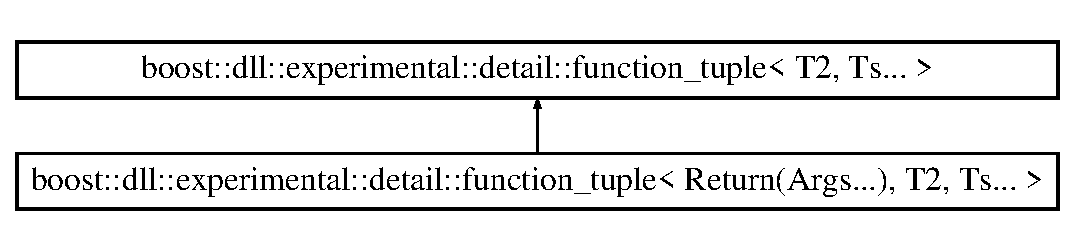
\includegraphics[height=2.000000cm]{a01468}
\end{center}
\end{figure}
\subsection*{Public Member Functions}
\begin{DoxyCompactItemize}
\item 
\mbox{\Hypertarget{a01468_a6afcd4f7aee21e0bceb780d950dc450d}\label{a01468_a6afcd4f7aee21e0bceb780d950dc450d}} 
constexpr {\bfseries function\+\_\+tuple} (Return($\ast$t)(Args...), T2 $\ast$t2, Ts $\ast$... ts)
\item 
\mbox{\Hypertarget{a01468_a7c7a12b0e9db6f25edead61adafbfd6e}\label{a01468_a7c7a12b0e9db6f25edead61adafbfd6e}} 
Return {\bfseries operator()} (Args...\+args) const
\end{DoxyCompactItemize}
\subsection*{Public Attributes}
\begin{DoxyCompactItemize}
\item 
\mbox{\Hypertarget{a01468_a3e05c0f04b51b4e787d64836bd179278}\label{a01468_a3e05c0f04b51b4e787d64836bd179278}} 
Return($\ast$ {\bfseries f\+\_\+} )(Args...)
\end{DoxyCompactItemize}


The documentation for this struct was generated from the following file\+:\begin{DoxyCompactItemize}
\item 
import\+\_\+mangled\+\_\+helpers.\+hpp\end{DoxyCompactItemize}

\hypertarget{a01472}{}\section{boost\+:\+:dll\+:\+:experimental\+:\+:detail\+:\+:function\+\_\+tuple$<$ Return(Args...)$>$ Struct Template Reference}
\label{a01472}\index{boost\+::dll\+::experimental\+::detail\+::function\+\_\+tuple$<$ Return(\+Args...)$>$@{boost\+::dll\+::experimental\+::detail\+::function\+\_\+tuple$<$ Return(\+Args...)$>$}}
\subsection*{Public Member Functions}
\begin{DoxyCompactItemize}
\item 
\mbox{\Hypertarget{a01472_ab85660385eab5c21aaa4e70317680ce5}\label{a01472_ab85660385eab5c21aaa4e70317680ce5}} 
constexpr {\bfseries function\+\_\+tuple} (Return($\ast$t)(Args...))
\item 
\mbox{\Hypertarget{a01472_a51f92c9e9f4909c86f179070f026c7f3}\label{a01472_a51f92c9e9f4909c86f179070f026c7f3}} 
Return {\bfseries operator()} (Args...\+args) const
\end{DoxyCompactItemize}
\subsection*{Public Attributes}
\begin{DoxyCompactItemize}
\item 
\mbox{\Hypertarget{a01472_a16864d5b5d7f82eba86c331ecc3fc5d0}\label{a01472_a16864d5b5d7f82eba86c331ecc3fc5d0}} 
Return($\ast$ {\bfseries f\+\_\+} )(Args...)
\end{DoxyCompactItemize}


The documentation for this struct was generated from the following file\+:\begin{DoxyCompactItemize}
\item 
import\+\_\+mangled\+\_\+helpers.\+hpp\end{DoxyCompactItemize}

\hypertarget{a01240}{}\section{xacc\+:\+:quantum\+:\+:Functional\+Gate\+Instruction\+Visitor Class Reference}
\label{a01240}\index{xacc\+::quantum\+::\+Functional\+Gate\+Instruction\+Visitor@{xacc\+::quantum\+::\+Functional\+Gate\+Instruction\+Visitor}}
Inheritance diagram for xacc\+:\+:quantum\+:\+:Functional\+Gate\+Instruction\+Visitor\+:\begin{figure}[H]
\begin{center}
\leavevmode
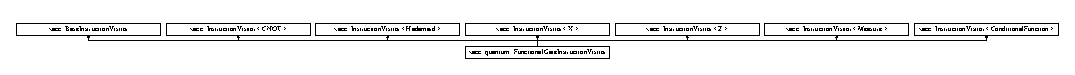
\includegraphics[height=0.563380cm]{a01240}
\end{center}
\end{figure}
\subsection*{Public Member Functions}
\begin{DoxyCompactItemize}
\item 
\mbox{\Hypertarget{a01240_a88d6b032e70cfa05f0a7bcee8dbc958a}\label{a01240_a88d6b032e70cfa05f0a7bcee8dbc958a}} 
{\footnotesize template$<$typename HF , typename C\+NF , typename XF , typename MF , typename ZF , typename CF $>$ }\\{\bfseries Functional\+Gate\+Instruction\+Visitor} (HF h, C\+NF cn, XF x, MF m, ZF z, CF c)
\item 
\mbox{\Hypertarget{a01240_ac5245d34429dc112e7cd0e371108fcb5}\label{a01240_ac5245d34429dc112e7cd0e371108fcb5}} 
void {\bfseries visit} (\hyperlink{a01308}{Hadamard} \&h)
\item 
\mbox{\Hypertarget{a01240_ad4eddafe8ca3906cd4aa5b98087a789a}\label{a01240_ad4eddafe8ca3906cd4aa5b98087a789a}} 
void {\bfseries visit} (\hyperlink{a01300}{C\+N\+OT} \&cn)
\item 
\mbox{\Hypertarget{a01240_ac5d184daee7e755c9ede67b34bc2d091}\label{a01240_ac5d184daee7e755c9ede67b34bc2d091}} 
void {\bfseries visit} (\hyperlink{a01320}{X} \&x)
\item 
\mbox{\Hypertarget{a01240_a4baf19da581fa9875739a227aba9cf60}\label{a01240_a4baf19da581fa9875739a227aba9cf60}} 
void {\bfseries visit} (\hyperlink{a01324}{Z} \&z)
\item 
\mbox{\Hypertarget{a01240_ad946faf8e2b6eff3e9e142907ec8e05a}\label{a01240_ad946faf8e2b6eff3e9e142907ec8e05a}} 
void {\bfseries visit} (\hyperlink{a01312}{Measure} \&m)
\item 
\mbox{\Hypertarget{a01240_a5cdb38902c241e7ae672a2631f1d61f3}\label{a01240_a5cdb38902c241e7ae672a2631f1d61f3}} 
void {\bfseries visit} (\hyperlink{a01304}{Conditional\+Function} \&c)
\end{DoxyCompactItemize}
\subsection*{Protected Attributes}
\begin{DoxyCompactItemize}
\item 
\mbox{\Hypertarget{a01240_a02f1401c9b0d1da801027f3bc0b5227e}\label{a01240_a02f1401c9b0d1da801027f3bc0b5227e}} 
std\+::function$<$ void(\hyperlink{a01308}{Hadamard} \&)$>$ {\bfseries h\+Action}
\item 
\mbox{\Hypertarget{a01240_a4d6bd8c2fd1af775ed08946942f60a0b}\label{a01240_a4d6bd8c2fd1af775ed08946942f60a0b}} 
std\+::function$<$ void(\hyperlink{a01300}{C\+N\+OT} \&)$>$ {\bfseries cnot\+Action}
\item 
\mbox{\Hypertarget{a01240_a9e0295434a2224b776609b057147a9af}\label{a01240_a9e0295434a2224b776609b057147a9af}} 
std\+::function$<$ void(\hyperlink{a01320}{X} \&)$>$ {\bfseries x\+Action}
\item 
\mbox{\Hypertarget{a01240_ae197f358e3d0777feb3656455e2ee672}\label{a01240_ae197f358e3d0777feb3656455e2ee672}} 
std\+::function$<$ void(\hyperlink{a01324}{Z} \&)$>$ {\bfseries z\+Action}
\item 
\mbox{\Hypertarget{a01240_a239748abedd67c7b30cad12e545d1926}\label{a01240_a239748abedd67c7b30cad12e545d1926}} 
std\+::function$<$ void(\hyperlink{a01312}{Measure} \&)$>$ {\bfseries measure\+Action}
\item 
\mbox{\Hypertarget{a01240_a5c0595a70b1f7ae50f3e29a985e249e9}\label{a01240_a5c0595a70b1f7ae50f3e29a985e249e9}} 
std\+::function$<$ void(\hyperlink{a01304}{Conditional\+Function} \&)$>$ {\bfseries cond\+Action}
\end{DoxyCompactItemize}


The documentation for this class was generated from the following file\+:\begin{DoxyCompactItemize}
\item 
Functional\+Gate\+Instruction\+Visitor.\+hpp\end{DoxyCompactItemize}

\hypertarget{a01272}{}\section{xacc\+:\+:quantum\+:\+:Gate\+Function Class Reference}
\label{a01272}\index{xacc\+::quantum\+::\+Gate\+Function@{xacc\+::quantum\+::\+Gate\+Function}}


{\ttfamily \#include $<$Gate\+Function.\+hpp$>$}

Inheritance diagram for xacc\+:\+:quantum\+:\+:Gate\+Function\+:\begin{figure}[H]
\begin{center}
\leavevmode
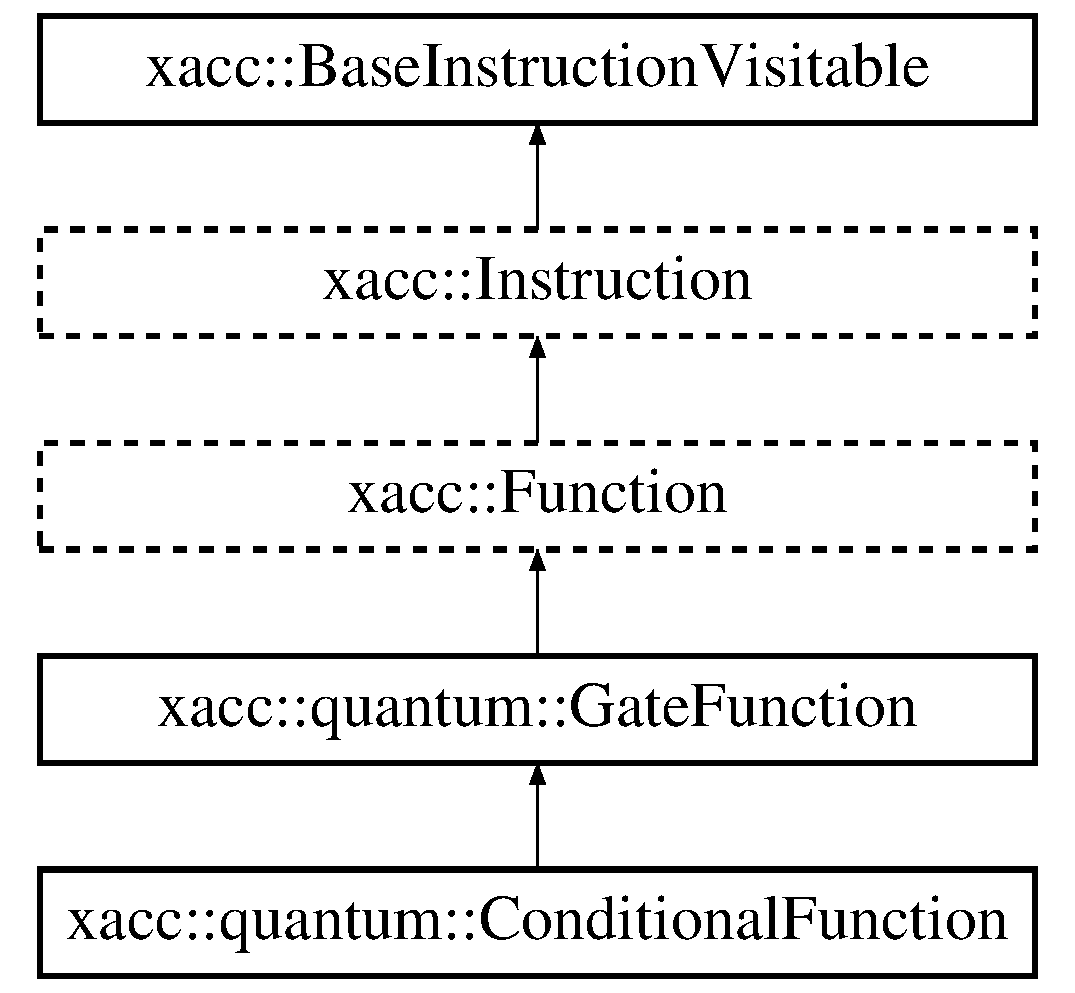
\includegraphics[height=5.000000cm]{a01272}
\end{center}
\end{figure}
\subsection*{Public Member Functions}
\begin{DoxyCompactItemize}
\item 
\hyperlink{a01272_a77545e72bd53268f609888654fcd8eee}{Gate\+Function} (const std\+::string \&name)
\item 
virtual const int \hyperlink{a01272_aa70b26156c060fec71316fe5e98bb102}{n\+Instructions} ()
\item 
virtual Inst\+Ptr \hyperlink{a01272_a841d656eed8aa9b4c0eec3f1da38069c}{get\+Instruction} (const int idx)
\item 
virtual std\+::list$<$ Inst\+Ptr $>$ \hyperlink{a01272_aebce6a9e64aed7f4aff86df752bacfe2}{get\+Instructions} ()
\item 
virtual void \hyperlink{a01272_a44ca35d081577de9ad2930f93c01e89d}{remove\+Instruction} (const int idx)
\item 
virtual void \hyperlink{a01272_a892fb69a10f0a7cb5abdab4cca61b80a}{add\+Instruction} (Inst\+Ptr instruction)
\item 
virtual void \hyperlink{a01272_a182fdfabbf546ae89e4f2384bafb45c9}{replace\+Instruction} (const int idx, Inst\+Ptr replacing\+Inst)
\item 
virtual const std\+::string \hyperlink{a01272_af42efb6191267164717d53c469e15d3a}{get\+Name} ()
\item 
virtual const std\+::vector$<$ int $>$ \hyperlink{a01272_aba03de68b76a9e120705c3c389c714a1}{bits} ()
\item 
virtual const std\+::string \hyperlink{a01272_aa1950776ae84bad2d0795a0441f910e7}{to\+String} (const std\+::string \&buffer\+Var\+Name)
\end{DoxyCompactItemize}
\subsection*{Protected Attributes}
\begin{DoxyCompactItemize}
\item 
std\+::string \hyperlink{a01272_aea17cb1ca610bb5b8eadb0642c32b937}{function\+Name}
\item 
\mbox{\Hypertarget{a01272_aa2334b23541206ed02023ec28f5e4ac7}\label{a01272_aa2334b23541206ed02023ec28f5e4ac7}} 
std\+::list$<$ Inst\+Ptr $>$ {\bfseries instructions}
\end{DoxyCompactItemize}
\subsection*{Additional Inherited Members}


\subsection{Detailed Description}
The \hyperlink{a01272}{Gate\+Function} is a Q\+Function for gate-\/model quantum computing. It is composed of Q\+Instructions that are themselves derivations of the \hyperlink{a01276}{Gate\+Instruction} class. 

\subsection{Constructor \& Destructor Documentation}
\mbox{\Hypertarget{a01272_a77545e72bd53268f609888654fcd8eee}\label{a01272_a77545e72bd53268f609888654fcd8eee}} 
\index{xacc\+::quantum\+::\+Gate\+Function@{xacc\+::quantum\+::\+Gate\+Function}!Gate\+Function@{Gate\+Function}}
\index{Gate\+Function@{Gate\+Function}!xacc\+::quantum\+::\+Gate\+Function@{xacc\+::quantum\+::\+Gate\+Function}}
\subsubsection{\texorpdfstring{Gate\+Function()}{GateFunction()}}
{\footnotesize\ttfamily xacc\+::quantum\+::\+Gate\+Function\+::\+Gate\+Function (\begin{DoxyParamCaption}\item[{const std\+::string \&}]{name }\end{DoxyParamCaption})\hspace{0.3cm}{\ttfamily [inline]}}

The constructor, takes the function unique id and its name.


\begin{DoxyParams}{Parameters}
{\em id} & \\
\hline
{\em name} & \\
\hline
\end{DoxyParams}


\subsection{Member Function Documentation}
\mbox{\Hypertarget{a01272_a892fb69a10f0a7cb5abdab4cca61b80a}\label{a01272_a892fb69a10f0a7cb5abdab4cca61b80a}} 
\index{xacc\+::quantum\+::\+Gate\+Function@{xacc\+::quantum\+::\+Gate\+Function}!add\+Instruction@{add\+Instruction}}
\index{add\+Instruction@{add\+Instruction}!xacc\+::quantum\+::\+Gate\+Function@{xacc\+::quantum\+::\+Gate\+Function}}
\subsubsection{\texorpdfstring{add\+Instruction()}{addInstruction()}}
{\footnotesize\ttfamily virtual void xacc\+::quantum\+::\+Gate\+Function\+::add\+Instruction (\begin{DoxyParamCaption}\item[{Inst\+Ptr}]{instruction }\end{DoxyParamCaption})\hspace{0.3cm}{\ttfamily [inline]}, {\ttfamily [virtual]}}

Add an instruction to this quantum intermediate representation.


\begin{DoxyParams}{Parameters}
{\em instruction} & \\
\hline
\end{DoxyParams}


Implements \hyperlink{a02456_aa8c9ec2d08be75c69399d4254b0216f5}{xacc\+::\+Function}.



Reimplemented in \hyperlink{a01304_a6aedad20f96390880efdc0a476b3273f}{xacc\+::quantum\+::\+Conditional\+Function}.

\mbox{\Hypertarget{a01272_aba03de68b76a9e120705c3c389c714a1}\label{a01272_aba03de68b76a9e120705c3c389c714a1}} 
\index{xacc\+::quantum\+::\+Gate\+Function@{xacc\+::quantum\+::\+Gate\+Function}!bits@{bits}}
\index{bits@{bits}!xacc\+::quantum\+::\+Gate\+Function@{xacc\+::quantum\+::\+Gate\+Function}}
\subsubsection{\texorpdfstring{bits()}{bits()}}
{\footnotesize\ttfamily virtual const std\+::vector$<$int$>$ xacc\+::quantum\+::\+Gate\+Function\+::bits (\begin{DoxyParamCaption}{ }\end{DoxyParamCaption})\hspace{0.3cm}{\ttfamily [inline]}, {\ttfamily [virtual]}}

Return the qubits this function acts on. \begin{DoxyReturn}{Returns}

\end{DoxyReturn}


Implements \hyperlink{a02460_a819f32e94c3e1c9e69a0061aaf8d86dc}{xacc\+::\+Instruction}.

\mbox{\Hypertarget{a01272_a841d656eed8aa9b4c0eec3f1da38069c}\label{a01272_a841d656eed8aa9b4c0eec3f1da38069c}} 
\index{xacc\+::quantum\+::\+Gate\+Function@{xacc\+::quantum\+::\+Gate\+Function}!get\+Instruction@{get\+Instruction}}
\index{get\+Instruction@{get\+Instruction}!xacc\+::quantum\+::\+Gate\+Function@{xacc\+::quantum\+::\+Gate\+Function}}
\subsubsection{\texorpdfstring{get\+Instruction()}{getInstruction()}}
{\footnotesize\ttfamily virtual Inst\+Ptr xacc\+::quantum\+::\+Gate\+Function\+::get\+Instruction (\begin{DoxyParamCaption}\item[{const int}]{idx }\end{DoxyParamCaption})\hspace{0.3cm}{\ttfamily [inline]}, {\ttfamily [virtual]}}

Return the \hyperlink{a02460}{Instruction} at the given index.


\begin{DoxyParams}{Parameters}
{\em idx} & The desired \hyperlink{a02460}{Instruction} index \\
\hline
\end{DoxyParams}
\begin{DoxyReturn}{Returns}
inst The instruction at the given index. 
\end{DoxyReturn}


Implements \hyperlink{a02456_afa549fc91b5a05f26d8139954a7e0ed5}{xacc\+::\+Function}.

\mbox{\Hypertarget{a01272_aebce6a9e64aed7f4aff86df752bacfe2}\label{a01272_aebce6a9e64aed7f4aff86df752bacfe2}} 
\index{xacc\+::quantum\+::\+Gate\+Function@{xacc\+::quantum\+::\+Gate\+Function}!get\+Instructions@{get\+Instructions}}
\index{get\+Instructions@{get\+Instructions}!xacc\+::quantum\+::\+Gate\+Function@{xacc\+::quantum\+::\+Gate\+Function}}
\subsubsection{\texorpdfstring{get\+Instructions()}{getInstructions()}}
{\footnotesize\ttfamily virtual std\+::list$<$Inst\+Ptr$>$ xacc\+::quantum\+::\+Gate\+Function\+::get\+Instructions (\begin{DoxyParamCaption}{ }\end{DoxyParamCaption})\hspace{0.3cm}{\ttfamily [inline]}, {\ttfamily [virtual]}}

Return all Instructions in this \hyperlink{a02456}{Function}

\begin{DoxyReturn}{Returns}
insts The list of this \hyperlink{a02456}{Function}\textquotesingle{}s Instructions 
\end{DoxyReturn}


Implements \hyperlink{a02456_aaf80bd3d49113a92b520785572663032}{xacc\+::\+Function}.

\mbox{\Hypertarget{a01272_af42efb6191267164717d53c469e15d3a}\label{a01272_af42efb6191267164717d53c469e15d3a}} 
\index{xacc\+::quantum\+::\+Gate\+Function@{xacc\+::quantum\+::\+Gate\+Function}!get\+Name@{get\+Name}}
\index{get\+Name@{get\+Name}!xacc\+::quantum\+::\+Gate\+Function@{xacc\+::quantum\+::\+Gate\+Function}}
\subsubsection{\texorpdfstring{get\+Name()}{getName()}}
{\footnotesize\ttfamily virtual const std\+::string xacc\+::quantum\+::\+Gate\+Function\+::get\+Name (\begin{DoxyParamCaption}{ }\end{DoxyParamCaption})\hspace{0.3cm}{\ttfamily [inline]}, {\ttfamily [virtual]}}

Return the name of this function \begin{DoxyReturn}{Returns}

\end{DoxyReturn}


Implements \hyperlink{a02460_ac7ff23f693e2276edbf3fdac5452792c}{xacc\+::\+Instruction}.

\mbox{\Hypertarget{a01272_aa70b26156c060fec71316fe5e98bb102}\label{a01272_aa70b26156c060fec71316fe5e98bb102}} 
\index{xacc\+::quantum\+::\+Gate\+Function@{xacc\+::quantum\+::\+Gate\+Function}!n\+Instructions@{n\+Instructions}}
\index{n\+Instructions@{n\+Instructions}!xacc\+::quantum\+::\+Gate\+Function@{xacc\+::quantum\+::\+Gate\+Function}}
\subsubsection{\texorpdfstring{n\+Instructions()}{nInstructions()}}
{\footnotesize\ttfamily virtual const int xacc\+::quantum\+::\+Gate\+Function\+::n\+Instructions (\begin{DoxyParamCaption}{ }\end{DoxyParamCaption})\hspace{0.3cm}{\ttfamily [inline]}, {\ttfamily [virtual]}}

Return the number of Instructions that this \hyperlink{a02456}{Function} contains.

\begin{DoxyReturn}{Returns}
n\+Inst The number of instructions 
\end{DoxyReturn}


Implements \hyperlink{a02456_a8901985525f59713e14c61713e07c086}{xacc\+::\+Function}.

\mbox{\Hypertarget{a01272_a44ca35d081577de9ad2930f93c01e89d}\label{a01272_a44ca35d081577de9ad2930f93c01e89d}} 
\index{xacc\+::quantum\+::\+Gate\+Function@{xacc\+::quantum\+::\+Gate\+Function}!remove\+Instruction@{remove\+Instruction}}
\index{remove\+Instruction@{remove\+Instruction}!xacc\+::quantum\+::\+Gate\+Function@{xacc\+::quantum\+::\+Gate\+Function}}
\subsubsection{\texorpdfstring{remove\+Instruction()}{removeInstruction()}}
{\footnotesize\ttfamily virtual void xacc\+::quantum\+::\+Gate\+Function\+::remove\+Instruction (\begin{DoxyParamCaption}\item[{const int}]{idx }\end{DoxyParamCaption})\hspace{0.3cm}{\ttfamily [inline]}, {\ttfamily [virtual]}}

Remove the \hyperlink{a02460}{Instruction} at the given index.


\begin{DoxyParams}{Parameters}
{\em idx} & The index of the \hyperlink{a02460}{Instruction} to remove. \\
\hline
\end{DoxyParams}


Implements \hyperlink{a02456_ab6478b09bb28e194bb555b3180737733}{xacc\+::\+Function}.

\mbox{\Hypertarget{a01272_a182fdfabbf546ae89e4f2384bafb45c9}\label{a01272_a182fdfabbf546ae89e4f2384bafb45c9}} 
\index{xacc\+::quantum\+::\+Gate\+Function@{xacc\+::quantum\+::\+Gate\+Function}!replace\+Instruction@{replace\+Instruction}}
\index{replace\+Instruction@{replace\+Instruction}!xacc\+::quantum\+::\+Gate\+Function@{xacc\+::quantum\+::\+Gate\+Function}}
\subsubsection{\texorpdfstring{replace\+Instruction()}{replaceInstruction()}}
{\footnotesize\ttfamily virtual void xacc\+::quantum\+::\+Gate\+Function\+::replace\+Instruction (\begin{DoxyParamCaption}\item[{const int}]{idx,  }\item[{Inst\+Ptr}]{replacing\+Inst }\end{DoxyParamCaption})\hspace{0.3cm}{\ttfamily [inline]}, {\ttfamily [virtual]}}

Replace the given current quantum instruction with the new replacing\+Inst quantum \hyperlink{a02460}{Instruction}.


\begin{DoxyParams}{Parameters}
{\em current\+Inst} & \\
\hline
{\em replacing\+Inst} & \\
\hline
\end{DoxyParams}


Implements \hyperlink{a02456_a2ef6a4923a6734f90f6ee3d94d263af0}{xacc\+::\+Function}.

\mbox{\Hypertarget{a01272_aa1950776ae84bad2d0795a0441f910e7}\label{a01272_aa1950776ae84bad2d0795a0441f910e7}} 
\index{xacc\+::quantum\+::\+Gate\+Function@{xacc\+::quantum\+::\+Gate\+Function}!to\+String@{to\+String}}
\index{to\+String@{to\+String}!xacc\+::quantum\+::\+Gate\+Function@{xacc\+::quantum\+::\+Gate\+Function}}
\subsubsection{\texorpdfstring{to\+String()}{toString()}}
{\footnotesize\ttfamily virtual const std\+::string xacc\+::quantum\+::\+Gate\+Function\+::to\+String (\begin{DoxyParamCaption}\item[{const std\+::string \&}]{buffer\+Var\+Name }\end{DoxyParamCaption})\hspace{0.3cm}{\ttfamily [inline]}, {\ttfamily [virtual]}}

Return an assembly-\/like string representation for this function . 
\begin{DoxyParams}{Parameters}
{\em buffer\+Var\+Name} & \\
\hline
\end{DoxyParams}
\begin{DoxyReturn}{Returns}

\end{DoxyReturn}


Implements \hyperlink{a02460_ae94c2d089908294c1d410b14c96817ae}{xacc\+::\+Instruction}.



Reimplemented in \hyperlink{a01304_aca7a5f849fece6fc28a904efee9a3370}{xacc\+::quantum\+::\+Conditional\+Function}.



\subsection{Member Data Documentation}
\mbox{\Hypertarget{a01272_aea17cb1ca610bb5b8eadb0642c32b937}\label{a01272_aea17cb1ca610bb5b8eadb0642c32b937}} 
\index{xacc\+::quantum\+::\+Gate\+Function@{xacc\+::quantum\+::\+Gate\+Function}!function\+Name@{function\+Name}}
\index{function\+Name@{function\+Name}!xacc\+::quantum\+::\+Gate\+Function@{xacc\+::quantum\+::\+Gate\+Function}}
\subsubsection{\texorpdfstring{function\+Name}{functionName}}
{\footnotesize\ttfamily std\+::string xacc\+::quantum\+::\+Gate\+Function\+::function\+Name\hspace{0.3cm}{\ttfamily [protected]}}

The name of this function 

The documentation for this class was generated from the following file\+:\begin{DoxyCompactItemize}
\item 
Gate\+Function.\+hpp\end{DoxyCompactItemize}

\hypertarget{a01276}{}\section{xacc\+:\+:quantum\+:\+:Gate\+Instruction Class Reference}
\label{a01276}\index{xacc\+::quantum\+::\+Gate\+Instruction@{xacc\+::quantum\+::\+Gate\+Instruction}}
Inheritance diagram for xacc\+:\+:quantum\+:\+:Gate\+Instruction\+:\begin{figure}[H]
\begin{center}
\leavevmode
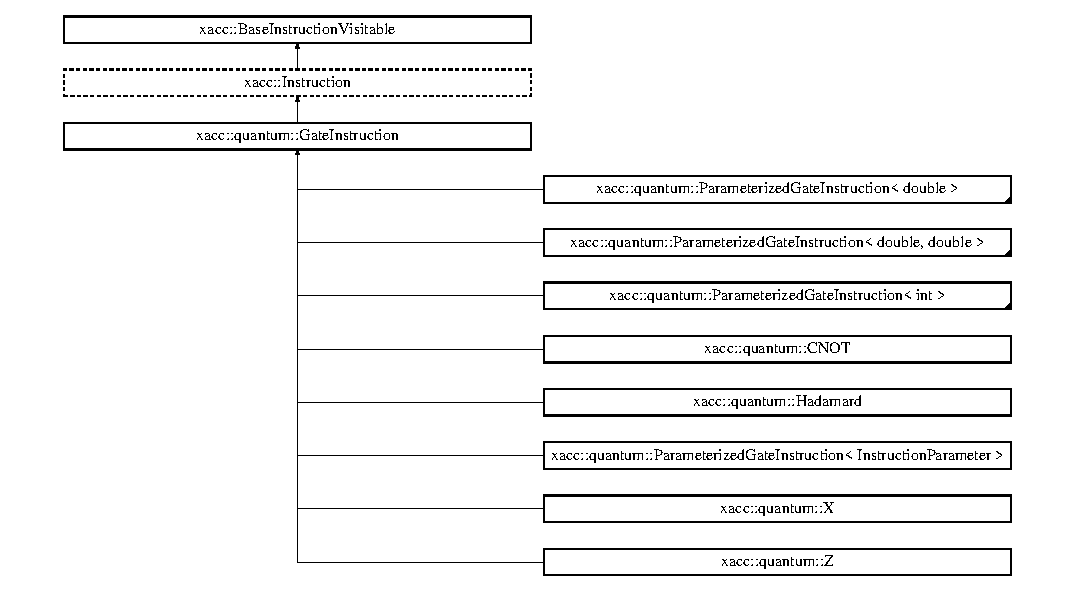
\includegraphics[height=7.512195cm]{a01276}
\end{center}
\end{figure}
\subsection*{Public Member Functions}
\begin{DoxyCompactItemize}
\item 
\mbox{\Hypertarget{a01276_a951ac3f44fcfbcf187bb73ba7438b472}\label{a01276_a951ac3f44fcfbcf187bb73ba7438b472}} 
{\bfseries Gate\+Instruction} (std\+::vector$<$ int $>$ qubts)
\item 
\hyperlink{a01276_a9b8543b79576c69ab8578ab6228134d7}{Gate\+Instruction} (std\+::string name, std\+::vector$<$ int $>$ qubts)
\item 
virtual const std\+::string \hyperlink{a01276_a0db03b9e46eeba1134f0ca2b83ccc842}{get\+Name} ()
\item 
virtual const std\+::vector$<$ int $>$ \hyperlink{a01276_ad32ad03dfc516e00093030e60178003d}{bits} ()
\item 
virtual const std\+::string \hyperlink{a01276_a089a5da67ff40ac1a6f56e64589822d9}{to\+String} (const std\+::string \&buffer\+Var\+Name)
\item 
virtual bool \hyperlink{a01276_a0a821be322b0c848b01c55f91fc8f484}{is\+Enabled} ()
\item 
virtual void \hyperlink{a01276_a63ce138dd71fb43d303f5600fefb7215}{disable} ()
\item 
virtual void \hyperlink{a01276_a7a80474b7fd465271b3313432db2e608}{enable} ()
\item 
virtual \hyperlink{a01276_ab8a75144074b27262fc33c77db4528b7}{$\sim$\+Gate\+Instruction} ()
\end{DoxyCompactItemize}
\subsection*{Protected Attributes}
\begin{DoxyCompactItemize}
\item 
std\+::string \hyperlink{a01276_a9961e6979139ced70300188cf2e4ad3f}{gate\+Name}
\item 
std\+::vector$<$ int $>$ \hyperlink{a01276_a2a56be6c2519ea65df4d06f4abae1393}{qbits}
\item 
\mbox{\Hypertarget{a01276_aa1039a127aa645a5c2206ef64e20b37a}\label{a01276_aa1039a127aa645a5c2206ef64e20b37a}} 
bool {\bfseries enabled} = true
\end{DoxyCompactItemize}
\subsection*{Additional Inherited Members}


\subsection{Constructor \& Destructor Documentation}
\mbox{\Hypertarget{a01276_a9b8543b79576c69ab8578ab6228134d7}\label{a01276_a9b8543b79576c69ab8578ab6228134d7}} 
\index{xacc\+::quantum\+::\+Gate\+Instruction@{xacc\+::quantum\+::\+Gate\+Instruction}!Gate\+Instruction@{Gate\+Instruction}}
\index{Gate\+Instruction@{Gate\+Instruction}!xacc\+::quantum\+::\+Gate\+Instruction@{xacc\+::quantum\+::\+Gate\+Instruction}}
\subsubsection{\texorpdfstring{Gate\+Instruction()}{GateInstruction()}}
{\footnotesize\ttfamily xacc\+::quantum\+::\+Gate\+Instruction\+::\+Gate\+Instruction (\begin{DoxyParamCaption}\item[{std\+::string}]{name,  }\item[{std\+::vector$<$ int $>$}]{qubts }\end{DoxyParamCaption})\hspace{0.3cm}{\ttfamily [inline]}}

The constructor, takes the id, name, layer, and qubits this instruction acts on.


\begin{DoxyParams}{Parameters}
{\em id} & \\
\hline
{\em layer} & \\
\hline
{\em name} & \\
\hline
{\em qubts} & \\
\hline
\end{DoxyParams}
\mbox{\Hypertarget{a01276_ab8a75144074b27262fc33c77db4528b7}\label{a01276_ab8a75144074b27262fc33c77db4528b7}} 
\index{xacc\+::quantum\+::\+Gate\+Instruction@{xacc\+::quantum\+::\+Gate\+Instruction}!````~Gate\+Instruction@{$\sim$\+Gate\+Instruction}}
\index{````~Gate\+Instruction@{$\sim$\+Gate\+Instruction}!xacc\+::quantum\+::\+Gate\+Instruction@{xacc\+::quantum\+::\+Gate\+Instruction}}
\subsubsection{\texorpdfstring{$\sim$\+Gate\+Instruction()}{~GateInstruction()}}
{\footnotesize\ttfamily virtual xacc\+::quantum\+::\+Gate\+Instruction\+::$\sim$\+Gate\+Instruction (\begin{DoxyParamCaption}{ }\end{DoxyParamCaption})\hspace{0.3cm}{\ttfamily [inline]}, {\ttfamily [virtual]}}

The destructor 

\subsection{Member Function Documentation}
\mbox{\Hypertarget{a01276_ad32ad03dfc516e00093030e60178003d}\label{a01276_ad32ad03dfc516e00093030e60178003d}} 
\index{xacc\+::quantum\+::\+Gate\+Instruction@{xacc\+::quantum\+::\+Gate\+Instruction}!bits@{bits}}
\index{bits@{bits}!xacc\+::quantum\+::\+Gate\+Instruction@{xacc\+::quantum\+::\+Gate\+Instruction}}
\subsubsection{\texorpdfstring{bits()}{bits()}}
{\footnotesize\ttfamily virtual const std\+::vector$<$int$>$ xacc\+::quantum\+::\+Gate\+Instruction\+::bits (\begin{DoxyParamCaption}{ }\end{DoxyParamCaption})\hspace{0.3cm}{\ttfamily [inline]}, {\ttfamily [virtual]}}

Return the list of qubits this instruction acts on. \begin{DoxyReturn}{Returns}

\end{DoxyReturn}


Implements \hyperlink{a02460_a819f32e94c3e1c9e69a0061aaf8d86dc}{xacc\+::\+Instruction}.

\mbox{\Hypertarget{a01276_a63ce138dd71fb43d303f5600fefb7215}\label{a01276_a63ce138dd71fb43d303f5600fefb7215}} 
\index{xacc\+::quantum\+::\+Gate\+Instruction@{xacc\+::quantum\+::\+Gate\+Instruction}!disable@{disable}}
\index{disable@{disable}!xacc\+::quantum\+::\+Gate\+Instruction@{xacc\+::quantum\+::\+Gate\+Instruction}}
\subsubsection{\texorpdfstring{disable()}{disable()}}
{\footnotesize\ttfamily virtual void xacc\+::quantum\+::\+Gate\+Instruction\+::disable (\begin{DoxyParamCaption}{ }\end{DoxyParamCaption})\hspace{0.3cm}{\ttfamily [inline]}, {\ttfamily [virtual]}}

Disable this \hyperlink{a02460}{Instruction} 

Reimplemented from \hyperlink{a02460_a6e528da15e05a94cc1d7db268c483271}{xacc\+::\+Instruction}.

\mbox{\Hypertarget{a01276_a7a80474b7fd465271b3313432db2e608}\label{a01276_a7a80474b7fd465271b3313432db2e608}} 
\index{xacc\+::quantum\+::\+Gate\+Instruction@{xacc\+::quantum\+::\+Gate\+Instruction}!enable@{enable}}
\index{enable@{enable}!xacc\+::quantum\+::\+Gate\+Instruction@{xacc\+::quantum\+::\+Gate\+Instruction}}
\subsubsection{\texorpdfstring{enable()}{enable()}}
{\footnotesize\ttfamily virtual void xacc\+::quantum\+::\+Gate\+Instruction\+::enable (\begin{DoxyParamCaption}{ }\end{DoxyParamCaption})\hspace{0.3cm}{\ttfamily [inline]}, {\ttfamily [virtual]}}

Enable this \hyperlink{a02460}{Instruction}. 

Reimplemented from \hyperlink{a02460_a0b4f2e5a591af28342a3c08e4305e24f}{xacc\+::\+Instruction}.

\mbox{\Hypertarget{a01276_a0db03b9e46eeba1134f0ca2b83ccc842}\label{a01276_a0db03b9e46eeba1134f0ca2b83ccc842}} 
\index{xacc\+::quantum\+::\+Gate\+Instruction@{xacc\+::quantum\+::\+Gate\+Instruction}!get\+Name@{get\+Name}}
\index{get\+Name@{get\+Name}!xacc\+::quantum\+::\+Gate\+Instruction@{xacc\+::quantum\+::\+Gate\+Instruction}}
\subsubsection{\texorpdfstring{get\+Name()}{getName()}}
{\footnotesize\ttfamily virtual const std\+::string xacc\+::quantum\+::\+Gate\+Instruction\+::get\+Name (\begin{DoxyParamCaption}{ }\end{DoxyParamCaption})\hspace{0.3cm}{\ttfamily [inline]}, {\ttfamily [virtual]}}

Return the instruction name. \begin{DoxyReturn}{Returns}

\end{DoxyReturn}


Implements \hyperlink{a02460_ac7ff23f693e2276edbf3fdac5452792c}{xacc\+::\+Instruction}.

\mbox{\Hypertarget{a01276_a0a821be322b0c848b01c55f91fc8f484}\label{a01276_a0a821be322b0c848b01c55f91fc8f484}} 
\index{xacc\+::quantum\+::\+Gate\+Instruction@{xacc\+::quantum\+::\+Gate\+Instruction}!is\+Enabled@{is\+Enabled}}
\index{is\+Enabled@{is\+Enabled}!xacc\+::quantum\+::\+Gate\+Instruction@{xacc\+::quantum\+::\+Gate\+Instruction}}
\subsubsection{\texorpdfstring{is\+Enabled()}{isEnabled()}}
{\footnotesize\ttfamily virtual bool xacc\+::quantum\+::\+Gate\+Instruction\+::is\+Enabled (\begin{DoxyParamCaption}{ }\end{DoxyParamCaption})\hspace{0.3cm}{\ttfamily [inline]}, {\ttfamily [virtual]}}

Returns true if this \hyperlink{a02460}{Instruction} is enabled

\begin{DoxyReturn}{Returns}
enabled True if this \hyperlink{a02460}{Instruction} is enabled. 
\end{DoxyReturn}


Reimplemented from \hyperlink{a02460_ad02a1cf7220577124720b7a51424cea7}{xacc\+::\+Instruction}.

\mbox{\Hypertarget{a01276_a089a5da67ff40ac1a6f56e64589822d9}\label{a01276_a089a5da67ff40ac1a6f56e64589822d9}} 
\index{xacc\+::quantum\+::\+Gate\+Instruction@{xacc\+::quantum\+::\+Gate\+Instruction}!to\+String@{to\+String}}
\index{to\+String@{to\+String}!xacc\+::quantum\+::\+Gate\+Instruction@{xacc\+::quantum\+::\+Gate\+Instruction}}
\subsubsection{\texorpdfstring{to\+String()}{toString()}}
{\footnotesize\ttfamily virtual const std\+::string xacc\+::quantum\+::\+Gate\+Instruction\+::to\+String (\begin{DoxyParamCaption}\item[{const std\+::string \&}]{buffer\+Var\+Name }\end{DoxyParamCaption})\hspace{0.3cm}{\ttfamily [inline]}, {\ttfamily [virtual]}}

Return this instruction\textquotesingle{}s assembly-\/like string representation. 
\begin{DoxyParams}{Parameters}
{\em buffer\+Var\+Name} & \\
\hline
\end{DoxyParams}
\begin{DoxyReturn}{Returns}

\end{DoxyReturn}


Implements \hyperlink{a02460_ae94c2d089908294c1d410b14c96817ae}{xacc\+::\+Instruction}.



Reimplemented in \hyperlink{a01280_aaccc4a20d58d2ac5c31abe7e325b8f77}{xacc\+::quantum\+::\+Parameterized\+Gate\+Instruction$<$ Instruction\+Parameter $>$}, \hyperlink{a01280_aaccc4a20d58d2ac5c31abe7e325b8f77}{xacc\+::quantum\+::\+Parameterized\+Gate\+Instruction$<$ double $>$}, \hyperlink{a01280_aaccc4a20d58d2ac5c31abe7e325b8f77}{xacc\+::quantum\+::\+Parameterized\+Gate\+Instruction$<$ int $>$}, \hyperlink{a01280_aaccc4a20d58d2ac5c31abe7e325b8f77}{xacc\+::quantum\+::\+Parameterized\+Gate\+Instruction$<$ double, double $>$}, and \hyperlink{a01312_a1c51a5d68294dcb2ba1a9fbea63a730f}{xacc\+::quantum\+::\+Measure}.



\subsection{Member Data Documentation}
\mbox{\Hypertarget{a01276_a9961e6979139ced70300188cf2e4ad3f}\label{a01276_a9961e6979139ced70300188cf2e4ad3f}} 
\index{xacc\+::quantum\+::\+Gate\+Instruction@{xacc\+::quantum\+::\+Gate\+Instruction}!gate\+Name@{gate\+Name}}
\index{gate\+Name@{gate\+Name}!xacc\+::quantum\+::\+Gate\+Instruction@{xacc\+::quantum\+::\+Gate\+Instruction}}
\subsubsection{\texorpdfstring{gate\+Name}{gateName}}
{\footnotesize\ttfamily std\+::string xacc\+::quantum\+::\+Gate\+Instruction\+::gate\+Name\hspace{0.3cm}{\ttfamily [protected]}}

Reference to this instructions name \mbox{\Hypertarget{a01276_a2a56be6c2519ea65df4d06f4abae1393}\label{a01276_a2a56be6c2519ea65df4d06f4abae1393}} 
\index{xacc\+::quantum\+::\+Gate\+Instruction@{xacc\+::quantum\+::\+Gate\+Instruction}!qbits@{qbits}}
\index{qbits@{qbits}!xacc\+::quantum\+::\+Gate\+Instruction@{xacc\+::quantum\+::\+Gate\+Instruction}}
\subsubsection{\texorpdfstring{qbits}{qbits}}
{\footnotesize\ttfamily std\+::vector$<$int$>$ xacc\+::quantum\+::\+Gate\+Instruction\+::qbits\hspace{0.3cm}{\ttfamily [protected]}}

Reference to the qubits this instruction acts on 

The documentation for this class was generated from the following file\+:\begin{DoxyCompactItemize}
\item 
Gate\+Instruction.\+hpp\end{DoxyCompactItemize}

\hypertarget{a01296}{}\section{xacc\+:\+:quantum\+:\+:Gate\+Q\+IR Class Reference}
\label{a01296}\index{xacc\+::quantum\+::\+Gate\+Q\+IR@{xacc\+::quantum\+::\+Gate\+Q\+IR}}


{\ttfamily \#include $<$Gate\+Q\+I\+R.\+hpp$>$}

Inheritance diagram for xacc\+:\+:quantum\+:\+:Gate\+Q\+IR\+:\begin{figure}[H]
\begin{center}
\leavevmode
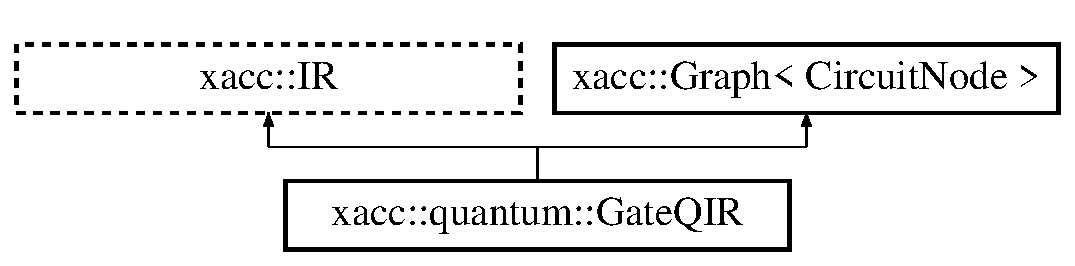
\includegraphics[height=2.000000cm]{a01296}
\end{center}
\end{figure}
\subsection*{Public Member Functions}
\begin{DoxyCompactItemize}
\item 
\hyperlink{a01296_afb99f610a6b123538c659169c131a634}{Gate\+Q\+IR} ()
\item 
virtual void \hyperlink{a01296_ad1ddd6105346dd9fc78648fd812285ed}{generate\+Graph} (const std\+::string \&kernel\+Name)
\item 
virtual void \hyperlink{a01296_aa6ed2cf2cbcfec8105c327a4fa95346f}{add\+Kernel} (std\+::shared\+\_\+ptr$<$ \hyperlink{a02456}{Function} $>$ kernel)
\item 
\mbox{\Hypertarget{a01296_aca6be85526b14f500e7f98954dd6da5c}\label{a01296_aca6be85526b14f500e7f98954dd6da5c}} 
virtual const int {\bfseries number\+Of\+Kernels} ()
\item 
virtual std\+::shared\+\_\+ptr$<$ \hyperlink{a02456}{Function} $>$ \hyperlink{a01296_a194758b6edcc3ae0c7fe8004f9bfe690}{get\+Kernel} (const std\+::string \&name)
\item 
virtual std\+::string \hyperlink{a01296_a7153f7e9f516d43af3d5d4f95d60bd86}{to\+Assembly\+String} (const std\+::string \&kernel\+Name, const std\+::string \&acc\+Buffer\+Var\+Name)
\item 
virtual void \hyperlink{a01296_a40e1d07e4dfd3794ef53fca3cdbdca61}{persist} (std\+::ostream \&out\+Stream)
\item 
virtual void \hyperlink{a01296_a07f26eeb362ac480d20da6cdc8c8fb39}{load} (std\+::istream \&in\+Stream)
\item 
virtual void \hyperlink{a01296_a26019e2f1e13e64645e29aee86ac58b1}{read} (std\+::istream \&stream)
\item 
virtual \hyperlink{a01296_ac88db03f1dd29e2d36aaa6c01a130008}{$\sim$\+Gate\+Q\+IR} ()
\end{DoxyCompactItemize}
\subsection*{Protected Attributes}
\begin{DoxyCompactItemize}
\item 
std\+::vector$<$ std\+::shared\+\_\+ptr$<$ \hyperlink{a02456}{Function} $>$ $>$ \hyperlink{a01296_ae75a4af0ce455eee1ce316c16426a661}{kernels}
\end{DoxyCompactItemize}


\subsection{Detailed Description}
The \hyperlink{a01296}{Gate\+Q\+IR} is an implementation of the Q\+IR for gate model quantum computing. It provides a \hyperlink{a02528}{Graph} node type that models a quantum circuit gate (\hyperlink{a01292}{Circuit\+Node}). 

\subsection{Constructor \& Destructor Documentation}
\mbox{\Hypertarget{a01296_afb99f610a6b123538c659169c131a634}\label{a01296_afb99f610a6b123538c659169c131a634}} 
\index{xacc\+::quantum\+::\+Gate\+Q\+IR@{xacc\+::quantum\+::\+Gate\+Q\+IR}!Gate\+Q\+IR@{Gate\+Q\+IR}}
\index{Gate\+Q\+IR@{Gate\+Q\+IR}!xacc\+::quantum\+::\+Gate\+Q\+IR@{xacc\+::quantum\+::\+Gate\+Q\+IR}}
\subsubsection{\texorpdfstring{Gate\+Q\+I\+R()}{GateQIR()}}
{\footnotesize\ttfamily xacc\+::quantum\+::\+Gate\+Q\+I\+R\+::\+Gate\+Q\+IR (\begin{DoxyParamCaption}{ }\end{DoxyParamCaption})\hspace{0.3cm}{\ttfamily [inline]}}

The nullary Constructor \mbox{\Hypertarget{a01296_ac88db03f1dd29e2d36aaa6c01a130008}\label{a01296_ac88db03f1dd29e2d36aaa6c01a130008}} 
\index{xacc\+::quantum\+::\+Gate\+Q\+IR@{xacc\+::quantum\+::\+Gate\+Q\+IR}!````~Gate\+Q\+IR@{$\sim$\+Gate\+Q\+IR}}
\index{````~Gate\+Q\+IR@{$\sim$\+Gate\+Q\+IR}!xacc\+::quantum\+::\+Gate\+Q\+IR@{xacc\+::quantum\+::\+Gate\+Q\+IR}}
\subsubsection{\texorpdfstring{$\sim$\+Gate\+Q\+I\+R()}{~GateQIR()}}
{\footnotesize\ttfamily virtual xacc\+::quantum\+::\+Gate\+Q\+I\+R\+::$\sim$\+Gate\+Q\+IR (\begin{DoxyParamCaption}{ }\end{DoxyParamCaption})\hspace{0.3cm}{\ttfamily [inline]}, {\ttfamily [virtual]}}

The destructor 

\subsection{Member Function Documentation}
\mbox{\Hypertarget{a01296_aa6ed2cf2cbcfec8105c327a4fa95346f}\label{a01296_aa6ed2cf2cbcfec8105c327a4fa95346f}} 
\index{xacc\+::quantum\+::\+Gate\+Q\+IR@{xacc\+::quantum\+::\+Gate\+Q\+IR}!add\+Kernel@{add\+Kernel}}
\index{add\+Kernel@{add\+Kernel}!xacc\+::quantum\+::\+Gate\+Q\+IR@{xacc\+::quantum\+::\+Gate\+Q\+IR}}
\subsubsection{\texorpdfstring{add\+Kernel()}{addKernel()}}
{\footnotesize\ttfamily virtual void xacc\+::quantum\+::\+Gate\+Q\+I\+R\+::add\+Kernel (\begin{DoxyParamCaption}\item[{std\+::shared\+\_\+ptr$<$ \hyperlink{a02456}{Function} $>$}]{kernel }\end{DoxyParamCaption})\hspace{0.3cm}{\ttfamily [inline]}, {\ttfamily [virtual]}}

Add a quantum function to this intermediate representation. 
\begin{DoxyParams}{Parameters}
{\em kernel} & \\
\hline
\end{DoxyParams}


Implements \hyperlink{a02480_abbbf8e6993c518597de32cd05d49d737}{xacc\+::\+IR}.

\mbox{\Hypertarget{a01296_ad1ddd6105346dd9fc78648fd812285ed}\label{a01296_ad1ddd6105346dd9fc78648fd812285ed}} 
\index{xacc\+::quantum\+::\+Gate\+Q\+IR@{xacc\+::quantum\+::\+Gate\+Q\+IR}!generate\+Graph@{generate\+Graph}}
\index{generate\+Graph@{generate\+Graph}!xacc\+::quantum\+::\+Gate\+Q\+IR@{xacc\+::quantum\+::\+Gate\+Q\+IR}}
\subsubsection{\texorpdfstring{generate\+Graph()}{generateGraph()}}
{\footnotesize\ttfamily void xacc\+::quantum\+::\+Gate\+Q\+I\+R\+::generate\+Graph (\begin{DoxyParamCaption}\item[{const std\+::string \&}]{kernel\+Name }\end{DoxyParamCaption})\hspace{0.3cm}{\ttfamily [virtual]}}

This method takes the list of quantum instructions that this Q\+IR contains and creates a graph representation of the quantum circuit. \mbox{\Hypertarget{a01296_a194758b6edcc3ae0c7fe8004f9bfe690}\label{a01296_a194758b6edcc3ae0c7fe8004f9bfe690}} 
\index{xacc\+::quantum\+::\+Gate\+Q\+IR@{xacc\+::quantum\+::\+Gate\+Q\+IR}!get\+Kernel@{get\+Kernel}}
\index{get\+Kernel@{get\+Kernel}!xacc\+::quantum\+::\+Gate\+Q\+IR@{xacc\+::quantum\+::\+Gate\+Q\+IR}}
\subsubsection{\texorpdfstring{get\+Kernel()}{getKernel()}}
{\footnotesize\ttfamily virtual std\+::shared\+\_\+ptr$<$\hyperlink{a02456}{Function}$>$ xacc\+::quantum\+::\+Gate\+Q\+I\+R\+::get\+Kernel (\begin{DoxyParamCaption}\item[{const std\+::string \&}]{name }\end{DoxyParamCaption})\hspace{0.3cm}{\ttfamily [inline]}, {\ttfamily [virtual]}}

Return the kernel with the given name.


\begin{DoxyParams}{Parameters}
{\em name} & The name of the kernel to return. \\
\hline
\end{DoxyParams}
\begin{DoxyReturn}{Returns}
kernel The kernel with given name. 
\end{DoxyReturn}


Implements \hyperlink{a02480_a6f49b4ba4b3a15142b04873284885f0d}{xacc\+::\+IR}.

\mbox{\Hypertarget{a01296_a07f26eeb362ac480d20da6cdc8c8fb39}\label{a01296_a07f26eeb362ac480d20da6cdc8c8fb39}} 
\index{xacc\+::quantum\+::\+Gate\+Q\+IR@{xacc\+::quantum\+::\+Gate\+Q\+IR}!load@{load}}
\index{load@{load}!xacc\+::quantum\+::\+Gate\+Q\+IR@{xacc\+::quantum\+::\+Gate\+Q\+IR}}
\subsubsection{\texorpdfstring{load()}{load()}}
{\footnotesize\ttfamily void xacc\+::quantum\+::\+Gate\+Q\+I\+R\+::load (\begin{DoxyParamCaption}\item[{std\+::istream \&}]{in\+Stream }\end{DoxyParamCaption})\hspace{0.3cm}{\ttfamily [virtual]}}

Create this \hyperlink{a02480}{IR} instance from the given input stream.


\begin{DoxyParams}{Parameters}
{\em in\+Stream} & \\
\hline
\end{DoxyParams}


Implements \hyperlink{a02480_a444c2e4dc0faac500fb70fa93997e9bc}{xacc\+::\+IR}.

\mbox{\Hypertarget{a01296_a40e1d07e4dfd3794ef53fca3cdbdca61}\label{a01296_a40e1d07e4dfd3794ef53fca3cdbdca61}} 
\index{xacc\+::quantum\+::\+Gate\+Q\+IR@{xacc\+::quantum\+::\+Gate\+Q\+IR}!persist@{persist}}
\index{persist@{persist}!xacc\+::quantum\+::\+Gate\+Q\+IR@{xacc\+::quantum\+::\+Gate\+Q\+IR}}
\subsubsection{\texorpdfstring{persist()}{persist()}}
{\footnotesize\ttfamily void xacc\+::quantum\+::\+Gate\+Q\+I\+R\+::persist (\begin{DoxyParamCaption}\item[{std\+::ostream \&}]{out\+Stream }\end{DoxyParamCaption})\hspace{0.3cm}{\ttfamily [virtual]}}

Persist this \hyperlink{a02480}{IR} instance to the given output stream.


\begin{DoxyParams}{Parameters}
{\em out\+Stream} & \\
\hline
\end{DoxyParams}


Implements \hyperlink{a02480_a414b72224d88473ad6190bb88102a3ea}{xacc\+::\+IR}.

\mbox{\Hypertarget{a01296_a26019e2f1e13e64645e29aee86ac58b1}\label{a01296_a26019e2f1e13e64645e29aee86ac58b1}} 
\index{xacc\+::quantum\+::\+Gate\+Q\+IR@{xacc\+::quantum\+::\+Gate\+Q\+IR}!read@{read}}
\index{read@{read}!xacc\+::quantum\+::\+Gate\+Q\+IR@{xacc\+::quantum\+::\+Gate\+Q\+IR}}
\subsubsection{\texorpdfstring{read()}{read()}}
{\footnotesize\ttfamily void xacc\+::quantum\+::\+Gate\+Q\+I\+R\+::read (\begin{DoxyParamCaption}\item[{std\+::istream \&}]{stream }\end{DoxyParamCaption})\hspace{0.3cm}{\ttfamily [virtual]}}

This is the implementation of the \hyperlink{a02528_abdd3e67dc08c223821d809bc8914164a}{Graph.\+read} method...

Read in a graphviz dot graph from the given input stream. This is left for subclasses.


\begin{DoxyParams}{Parameters}
{\em stream} & \\
\hline
\end{DoxyParams}


Reimplemented from \hyperlink{a02528_abdd3e67dc08c223821d809bc8914164a}{xacc\+::\+Graph$<$ Circuit\+Node $>$}.

\mbox{\Hypertarget{a01296_a7153f7e9f516d43af3d5d4f95d60bd86}\label{a01296_a7153f7e9f516d43af3d5d4f95d60bd86}} 
\index{xacc\+::quantum\+::\+Gate\+Q\+IR@{xacc\+::quantum\+::\+Gate\+Q\+IR}!to\+Assembly\+String@{to\+Assembly\+String}}
\index{to\+Assembly\+String@{to\+Assembly\+String}!xacc\+::quantum\+::\+Gate\+Q\+IR@{xacc\+::quantum\+::\+Gate\+Q\+IR}}
\subsubsection{\texorpdfstring{to\+Assembly\+String()}{toAssemblyString()}}
{\footnotesize\ttfamily std\+::string xacc\+::quantum\+::\+Gate\+Q\+I\+R\+::to\+Assembly\+String (\begin{DoxyParamCaption}\item[{const std\+::string \&}]{kernel\+Name,  }\item[{const std\+::string \&}]{acc\+Buffer\+Var\+Name }\end{DoxyParamCaption})\hspace{0.3cm}{\ttfamily [virtual]}}

Return a string representation of this intermediate representation \begin{DoxyReturn}{Returns}

\end{DoxyReturn}


Implements \hyperlink{a02480_a8356cdff1919b88eabeb84fd7450cdb6}{xacc\+::\+IR}.



\subsection{Member Data Documentation}
\mbox{\Hypertarget{a01296_ae75a4af0ce455eee1ce316c16426a661}\label{a01296_ae75a4af0ce455eee1ce316c16426a661}} 
\index{xacc\+::quantum\+::\+Gate\+Q\+IR@{xacc\+::quantum\+::\+Gate\+Q\+IR}!kernels@{kernels}}
\index{kernels@{kernels}!xacc\+::quantum\+::\+Gate\+Q\+IR@{xacc\+::quantum\+::\+Gate\+Q\+IR}}
\subsubsection{\texorpdfstring{kernels}{kernels}}
{\footnotesize\ttfamily std\+::vector$<$std\+::shared\+\_\+ptr$<$\hyperlink{a02456}{Function}$>$ $>$ xacc\+::quantum\+::\+Gate\+Q\+I\+R\+::kernels\hspace{0.3cm}{\ttfamily [protected]}}

Reference to this Q\+IR\textquotesingle{}s list of quantum functions 

The documentation for this class was generated from the following files\+:\begin{DoxyCompactItemize}
\item 
Gate\+Q\+I\+R.\+hpp\item 
Gate\+Q\+I\+R.\+cpp\end{DoxyCompactItemize}

\hypertarget{a02076}{}\section{Generic\+Array$<$ Const, ValueT $>$ Class Template Reference}
\label{a02076}\index{Generic\+Array$<$ Const, Value\+T $>$@{Generic\+Array$<$ Const, Value\+T $>$}}


Helper class for accessing Value of array type.  




{\ttfamily \#include $<$document.\+h$>$}

\subsection*{Public Types}
\begin{DoxyCompactItemize}
\item 
\mbox{\Hypertarget{a02076_a84f0b14518bc5cc44b4ff76a7d5ef81b}\label{a02076_a84f0b14518bc5cc44b4ff76a7d5ef81b}} 
typedef \hyperlink{a02076}{Generic\+Array}$<$ true, ValueT $>$ {\bfseries Const\+Array}
\item 
\mbox{\Hypertarget{a02076_a6683902e86c051c2319e873537dca7b1}\label{a02076_a6683902e86c051c2319e873537dca7b1}} 
typedef \hyperlink{a02076}{Generic\+Array}$<$ false, ValueT $>$ {\bfseries Array}
\item 
\mbox{\Hypertarget{a02076_aecea8be3dca6799bc523f4bffd221839}\label{a02076_aecea8be3dca6799bc523f4bffd221839}} 
typedef ValueT {\bfseries Plain\+Type}
\item 
\mbox{\Hypertarget{a02076_a93e53f38a99fc5167eb2a28653de64ed}\label{a02076_a93e53f38a99fc5167eb2a28653de64ed}} 
typedef internal\+::\+Maybe\+Add\+Const$<$ Const, Plain\+Type $>$\+::\hyperlink{a00560_a1d1cfd8ffb84e947f82999c682b666a7}{Type} {\bfseries Value\+Type}
\item 
\mbox{\Hypertarget{a02076_afc6ad62c3f00531fa378db266182704a}\label{a02076_afc6ad62c3f00531fa378db266182704a}} 
typedef Value\+Type $\ast$ {\bfseries Value\+Iterator}
\item 
\mbox{\Hypertarget{a02076_a1cd7bb3e75ccfeed3e8b0a6bb5563d68}\label{a02076_a1cd7bb3e75ccfeed3e8b0a6bb5563d68}} 
typedef const ValueT $\ast$ {\bfseries Const\+Value\+Iterator}
\item 
\mbox{\Hypertarget{a02076_af9cdc12de03c742b9c33dfc172756b97}\label{a02076_af9cdc12de03c742b9c33dfc172756b97}} 
typedef Value\+Type\+::\+Allocator\+Type {\bfseries Allocator\+Type}
\item 
\mbox{\Hypertarget{a02076_a8dcb9e2a2e103ce1051c16a7486465b9}\label{a02076_a8dcb9e2a2e103ce1051c16a7486465b9}} 
typedef Value\+Type\+::\+String\+Ref\+Type {\bfseries String\+Ref\+Type}
\end{DoxyCompactItemize}
\subsection*{Public Member Functions}
\begin{DoxyCompactItemize}
\item 
\mbox{\Hypertarget{a02076_aa589d897a194b349d5053391a6f1491d}\label{a02076_aa589d897a194b349d5053391a6f1491d}} 
{\bfseries Generic\+Array} (const \hyperlink{a02076}{Generic\+Array} \&rhs)
\item 
\mbox{\Hypertarget{a02076_addbff152092d0998b2c550bd575f4b83}\label{a02076_addbff152092d0998b2c550bd575f4b83}} 
\hyperlink{a02076}{Generic\+Array} \& {\bfseries operator=} (const \hyperlink{a02076}{Generic\+Array} \&rhs)
\item 
\mbox{\Hypertarget{a02076_a62d5b7f423edc2141cd4524c7dfd138b}\label{a02076_a62d5b7f423edc2141cd4524c7dfd138b}} 
\hyperlink{a00560_a5ed6e6e67250fadbd041127e6386dcb5}{Size\+Type} {\bfseries Size} () const
\item 
\mbox{\Hypertarget{a02076_ab385434ab7a99de7a0a17e5ee7e09d7f}\label{a02076_ab385434ab7a99de7a0a17e5ee7e09d7f}} 
\hyperlink{a00560_a5ed6e6e67250fadbd041127e6386dcb5}{Size\+Type} {\bfseries Capacity} () const
\item 
\mbox{\Hypertarget{a02076_af09e3aaeaeeb5fd825d79cc6663dfcf5}\label{a02076_af09e3aaeaeeb5fd825d79cc6663dfcf5}} 
bool {\bfseries Empty} () const
\item 
\mbox{\Hypertarget{a02076_a5e6c158ff76ab8a8ed568fa486e63c80}\label{a02076_a5e6c158ff76ab8a8ed568fa486e63c80}} 
void {\bfseries Clear} () const
\item 
\mbox{\Hypertarget{a02076_aa185d997e7787e9b4f624d5de592b886}\label{a02076_aa185d997e7787e9b4f624d5de592b886}} 
Value\+Type \& {\bfseries operator\mbox{[}$\,$\mbox{]}} (\hyperlink{a00560_a5ed6e6e67250fadbd041127e6386dcb5}{Size\+Type} index) const
\item 
\mbox{\Hypertarget{a02076_a3efaa020b29ceed9c1a03465676a32a7}\label{a02076_a3efaa020b29ceed9c1a03465676a32a7}} 
Value\+Iterator {\bfseries Begin} () const
\item 
\mbox{\Hypertarget{a02076_a396f83d328f4879225106ea14b1dca84}\label{a02076_a396f83d328f4879225106ea14b1dca84}} 
Value\+Iterator {\bfseries End} () const
\item 
\mbox{\Hypertarget{a02076_a7c74901e8e2174fe4661f4848995f355}\label{a02076_a7c74901e8e2174fe4661f4848995f355}} 
\hyperlink{a02076}{Generic\+Array} {\bfseries Reserve} (\hyperlink{a00560_a5ed6e6e67250fadbd041127e6386dcb5}{Size\+Type} new\+Capacity, Allocator\+Type \&allocator) const
\item 
\mbox{\Hypertarget{a02076_a2ed88f0630c044bad695a127a866c348}\label{a02076_a2ed88f0630c044bad695a127a866c348}} 
\hyperlink{a02076}{Generic\+Array} {\bfseries Push\+Back} (Value\+Type \&value, Allocator\+Type \&allocator) const
\item 
\mbox{\Hypertarget{a02076_ae599de6aee1167648085672b79dd6bcc}\label{a02076_ae599de6aee1167648085672b79dd6bcc}} 
\hyperlink{a02076}{Generic\+Array} {\bfseries Push\+Back} (String\+Ref\+Type value, Allocator\+Type \&allocator) const
\item 
\mbox{\Hypertarget{a02076_a12adff0c1e11aa3be6f4160015a65df0}\label{a02076_a12adff0c1e11aa3be6f4160015a65df0}} 
{\footnotesize template$<$typename T $>$ }\\{\bfseries R\+A\+P\+I\+D\+J\+S\+O\+N\+\_\+\+D\+I\+S\+A\+B\+L\+E\+I\+F\+\_\+\+R\+E\+T\+U\+RN} ((internal\+::\+Or\+Expr$<$ internal\+::\+Is\+Pointer$<$ T $>$, \hyperlink{a02020}{internal\+::\+Is\+Generic\+Value}$<$ T $>$ $>$),(const \hyperlink{a02076}{Generic\+Array} \&)) Push\+Back(T value
\item 
\mbox{\Hypertarget{a02076_afd1c75a82d2fc4366cde18256962edf6}\label{a02076_afd1c75a82d2fc4366cde18256962edf6}} 
\hyperlink{a02076}{Generic\+Array} {\bfseries Pop\+Back} () const
\item 
\mbox{\Hypertarget{a02076_aefa57a363accf2ade867583771f8a54b}\label{a02076_aefa57a363accf2ade867583771f8a54b}} 
Value\+Iterator {\bfseries Erase} (Const\+Value\+Iterator pos) const
\item 
\mbox{\Hypertarget{a02076_ac1be0c701ad3aaf0570a8a1ffc715fd5}\label{a02076_ac1be0c701ad3aaf0570a8a1ffc715fd5}} 
Value\+Iterator {\bfseries Erase} (Const\+Value\+Iterator first, Const\+Value\+Iterator last) const
\end{DoxyCompactItemize}
\subsection*{Public Attributes}
\begin{DoxyCompactItemize}
\item 
\mbox{\Hypertarget{a02076_a25d2ed55daa117c41db6a5b3f87e9ddc}\label{a02076_a25d2ed55daa117c41db6a5b3f87e9ddc}} 
Allocator\+Type \&allocator {\bfseries const} \{ value\+\_\+.\+Push\+Back(value, allocator)
\item 
\mbox{\Hypertarget{a02076_aef8b7baa9ec5cd68d8951fa8bad85217}\label{a02076_aef8b7baa9ec5cd68d8951fa8bad85217}} 
return $\ast$ {\bfseries this}
\end{DoxyCompactItemize}
\subsection*{Friends}
\begin{DoxyCompactItemize}
\item 
\mbox{\Hypertarget{a02076_a899449e1a645b5e377af059fb61113d8}\label{a02076_a899449e1a645b5e377af059fb61113d8}} 
{\footnotesize template$<$typename , typename $>$ }\\class {\bfseries Generic\+Value}
\end{DoxyCompactItemize}


\subsection{Detailed Description}
\subsubsection*{template$<$bool Const, typename ValueT$>$\newline
class Generic\+Array$<$ Const, Value\+T $>$}

Helper class for accessing Value of array type. 

Instance of this helper class is obtained by {\ttfamily Generic\+Value\+::\+Get\+Array()}. In addition to all A\+P\+Is for array type, it provides range-\/based for loop if {\ttfamily R\+A\+P\+I\+D\+J\+S\+O\+N\+\_\+\+H\+A\+S\+\_\+\+C\+X\+X11\+\_\+\+R\+A\+N\+G\+E\+\_\+\+F\+OR=1}. 

The documentation for this class was generated from the following file\+:\begin{DoxyCompactItemize}
\item 
\hyperlink{a00476}{document.\+h}\end{DoxyCompactItemize}

\hypertarget{a01996}{}\section{Generic\+Document$<$ Encoding, Allocator, Stack\+Allocator $>$ Class Template Reference}
\label{a01996}\index{Generic\+Document$<$ Encoding, Allocator, Stack\+Allocator $>$@{Generic\+Document$<$ Encoding, Allocator, Stack\+Allocator $>$}}


A document for parsing J\+S\+ON text as D\+OM.  




{\ttfamily \#include $<$document.\+h$>$}

Inheritance diagram for Generic\+Document$<$ Encoding, Allocator, Stack\+Allocator $>$\+:\begin{figure}[H]
\begin{center}
\leavevmode
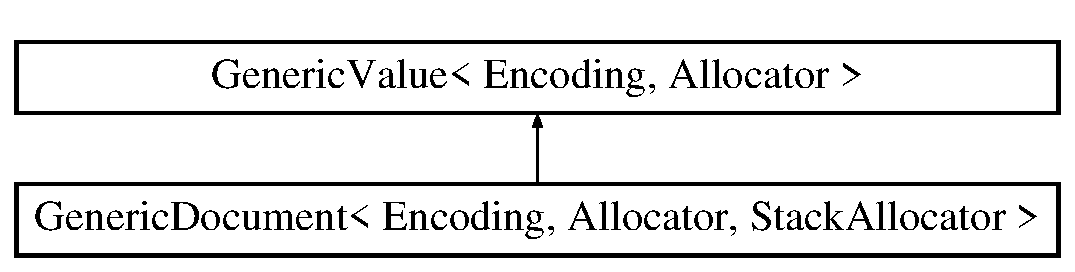
\includegraphics[height=2.000000cm]{a01996}
\end{center}
\end{figure}
\subsection*{Public Types}
\begin{DoxyCompactItemize}
\item 
\mbox{\Hypertarget{a01996_a6f5b0b7b6626508d094ae67490269700}\label{a01996_a6f5b0b7b6626508d094ae67490269700}} 
typedef Encoding\+::\+Ch \hyperlink{a01996_a6f5b0b7b6626508d094ae67490269700}{Ch}
\begin{DoxyCompactList}\small\item\em Character type derived from Encoding. \end{DoxyCompactList}\item 
\mbox{\Hypertarget{a01996_a8936205dc215dda029060d7e835e0549}\label{a01996_a8936205dc215dda029060d7e835e0549}} 
typedef \hyperlink{a01992}{Generic\+Value}$<$ Encoding, Allocator $>$ \hyperlink{a01996_a8936205dc215dda029060d7e835e0549}{Value\+Type}
\begin{DoxyCompactList}\small\item\em Value type of the document. \end{DoxyCompactList}\item 
\mbox{\Hypertarget{a01996_a35155b912da66ced38d22e2551364c57}\label{a01996_a35155b912da66ced38d22e2551364c57}} 
typedef Allocator \hyperlink{a01996_a35155b912da66ced38d22e2551364c57}{Allocator\+Type}
\begin{DoxyCompactList}\small\item\em Allocator type from template parameter. \end{DoxyCompactList}\end{DoxyCompactItemize}
\subsection*{Public Member Functions}
\begin{DoxyCompactItemize}
\item 
\hyperlink{a01996_a3da21e72ec8f26b9da77d86cc1d41cdd}{Generic\+Document} (\hyperlink{a00560_a1d1cfd8ffb84e947f82999c682b666a7}{Type} type, Allocator $\ast$allocator=0, size\+\_\+t stack\+Capacity=k\+Default\+Stack\+Capacity, Stack\+Allocator $\ast$stack\+Allocator=0)
\begin{DoxyCompactList}\small\item\em Constructor. \end{DoxyCompactList}\item 
\hyperlink{a01996_a6b1c313ad538cafc4d23d4bd5f97178c}{Generic\+Document} (Allocator $\ast$allocator=0, size\+\_\+t stack\+Capacity=k\+Default\+Stack\+Capacity, Stack\+Allocator $\ast$stack\+Allocator=0)
\begin{DoxyCompactList}\small\item\em Constructor. \end{DoxyCompactList}\item 
\hyperlink{a01996}{Generic\+Document} \& \hyperlink{a01996_a6290e1290fad74177625af5938c0c58f}{Swap} (\hyperlink{a01996}{Generic\+Document} \&rhs) R\+A\+P\+I\+D\+J\+S\+O\+N\+\_\+\+N\+O\+E\+X\+C\+E\+PT
\begin{DoxyCompactList}\small\item\em Exchange the contents of this document with those of another. \end{DoxyCompactList}\item 
{\footnotesize template$<$typename Generator $>$ }\\\hyperlink{a01996}{Generic\+Document} \& \hyperlink{a01996_a36fbc7d0a9595d26e0d2c8859d207d1f}{Populate} (Generator \&g)
\begin{DoxyCompactList}\small\item\em Populate this document by a generator which produces S\+AX events. \end{DoxyCompactList}\item 
\mbox{\Hypertarget{a01996_aa4609d6b19f86aec1a6b96edf2c27686}\label{a01996_aa4609d6b19f86aec1a6b96edf2c27686}} 
Allocator \& \hyperlink{a01996_aa4609d6b19f86aec1a6b96edf2c27686}{Get\+Allocator} ()
\begin{DoxyCompactList}\small\item\em Get the allocator of this document. \end{DoxyCompactList}\item 
\mbox{\Hypertarget{a01996_a9e2e543c326b8b981d4f2c3d6793d15b}\label{a01996_a9e2e543c326b8b981d4f2c3d6793d15b}} 
size\+\_\+t \hyperlink{a01996_a9e2e543c326b8b981d4f2c3d6793d15b}{Get\+Stack\+Capacity} () const
\begin{DoxyCompactList}\small\item\em Get the capacity of stack in bytes. \end{DoxyCompactList}\item 
\mbox{\Hypertarget{a01996_a87dc7f66b2b92660b8a43546733f9df2}\label{a01996_a87dc7f66b2b92660b8a43546733f9df2}} 
bool {\bfseries Null} ()
\item 
\mbox{\Hypertarget{a01996_a4c44780642518dd34bd241a1ea0ceaf1}\label{a01996_a4c44780642518dd34bd241a1ea0ceaf1}} 
bool {\bfseries Bool} (bool b)
\item 
\mbox{\Hypertarget{a01996_a8cc986266becaa268474c607489745c7}\label{a01996_a8cc986266becaa268474c607489745c7}} 
bool {\bfseries Int} (int i)
\item 
\mbox{\Hypertarget{a01996_a530dd899a04a00ba74f52507b488d2c1}\label{a01996_a530dd899a04a00ba74f52507b488d2c1}} 
bool {\bfseries Uint} (unsigned i)
\item 
\mbox{\Hypertarget{a01996_a934b1b7a7ed89917615a5410db77a942}\label{a01996_a934b1b7a7ed89917615a5410db77a942}} 
bool {\bfseries Int64} (int64\+\_\+t i)
\item 
\mbox{\Hypertarget{a01996_a50ac3451a1afd0ce248dcc023d5e09e8}\label{a01996_a50ac3451a1afd0ce248dcc023d5e09e8}} 
bool {\bfseries Uint64} (uint64\+\_\+t i)
\item 
\mbox{\Hypertarget{a01996_a934bf7a5d1ff062ab079756d842e4f6b}\label{a01996_a934bf7a5d1ff062ab079756d842e4f6b}} 
bool {\bfseries Double} (double d)
\item 
\mbox{\Hypertarget{a01996_af703994dec5af6ef049a24b5243aceab}\label{a01996_af703994dec5af6ef049a24b5243aceab}} 
bool {\bfseries Raw\+Number} (const \hyperlink{a01992_ade0e0ce64ccd5d852da57a35e720bafb}{Ch} $\ast$str, \hyperlink{a00560_a5ed6e6e67250fadbd041127e6386dcb5}{Size\+Type} length, bool copy)
\item 
\mbox{\Hypertarget{a01996_ad319fcc9e13606b6795424b9374a7398}\label{a01996_ad319fcc9e13606b6795424b9374a7398}} 
bool {\bfseries String} (const \hyperlink{a01992_ade0e0ce64ccd5d852da57a35e720bafb}{Ch} $\ast$str, \hyperlink{a00560_a5ed6e6e67250fadbd041127e6386dcb5}{Size\+Type} length, bool copy)
\item 
\mbox{\Hypertarget{a01996_abb1417fde52cc34cb340e3b50a3295da}\label{a01996_abb1417fde52cc34cb340e3b50a3295da}} 
bool {\bfseries Start\+Object} ()
\item 
\mbox{\Hypertarget{a01996_a600d0950baabbcab11197cacb1459c7a}\label{a01996_a600d0950baabbcab11197cacb1459c7a}} 
bool {\bfseries Key} (const \hyperlink{a01992_ade0e0ce64ccd5d852da57a35e720bafb}{Ch} $\ast$str, \hyperlink{a00560_a5ed6e6e67250fadbd041127e6386dcb5}{Size\+Type} length, bool copy)
\item 
\mbox{\Hypertarget{a01996_a42f2df68f9c9d8b88a15b609716867d9}\label{a01996_a42f2df68f9c9d8b88a15b609716867d9}} 
bool {\bfseries End\+Object} (\hyperlink{a00560_a5ed6e6e67250fadbd041127e6386dcb5}{Size\+Type} member\+Count)
\item 
\mbox{\Hypertarget{a01996_ae12c513c61745ae731a47b1ca33db063}\label{a01996_ae12c513c61745ae731a47b1ca33db063}} 
bool {\bfseries Start\+Array} ()
\item 
\mbox{\Hypertarget{a01996_a14097c833bed1a9c7be064ea619c887f}\label{a01996_a14097c833bed1a9c7be064ea619c887f}} 
bool {\bfseries End\+Array} (\hyperlink{a00560_a5ed6e6e67250fadbd041127e6386dcb5}{Size\+Type} element\+Count)
\end{DoxyCompactItemize}
\begin{Indent}\textbf{ Parse from stream}\par
\begin{DoxyCompactItemize}
\item 
{\footnotesize template$<$unsigned parse\+Flags, typename Source\+Encoding , typename Input\+Stream $>$ }\\\hyperlink{a01996}{Generic\+Document} \& \hyperlink{a01996_afe94c0abc83a20f2d7dc1ba7677e6238}{Parse\+Stream} (Input\+Stream \&is)
\begin{DoxyCompactList}\small\item\em Parse J\+S\+ON text from an input stream (with Encoding conversion) \end{DoxyCompactList}\item 
{\footnotesize template$<$unsigned parse\+Flags, typename Input\+Stream $>$ }\\\hyperlink{a01996}{Generic\+Document} \& \hyperlink{a01996_a6e154066c6f5024b91aaab25e03700e3}{Parse\+Stream} (Input\+Stream \&is)
\begin{DoxyCompactList}\small\item\em Parse J\+S\+ON text from an input stream. \end{DoxyCompactList}\item 
{\footnotesize template$<$typename Input\+Stream $>$ }\\\hyperlink{a01996}{Generic\+Document} \& \hyperlink{a01996_abe07ededbe9aaceb0058e3d254892b71}{Parse\+Stream} (Input\+Stream \&is)
\begin{DoxyCompactList}\small\item\em Parse J\+S\+ON text from an input stream (with \hyperlink{a00563_ab7be7dabe6ffcba60fad441505583450a9104b0946d648e9467cb7a967401ec80}{k\+Parse\+Default\+Flags}) \end{DoxyCompactList}\end{DoxyCompactItemize}
\end{Indent}
\begin{Indent}\textbf{ Parse in-\/place from mutable string}\par
\begin{DoxyCompactItemize}
\item 
{\footnotesize template$<$unsigned parse\+Flags$>$ }\\\hyperlink{a01996}{Generic\+Document} \& \hyperlink{a01996_a301f8f297a5a0da4b6be5459ad766f75}{Parse\+Insitu} (\hyperlink{a01992_ade0e0ce64ccd5d852da57a35e720bafb}{Ch} $\ast$str)
\begin{DoxyCompactList}\small\item\em Parse J\+S\+ON text from a mutable string. \end{DoxyCompactList}\item 
\hyperlink{a01996}{Generic\+Document} \& \hyperlink{a01996_a81922881357539d5482d31aea14b5664}{Parse\+Insitu} (\hyperlink{a01992_ade0e0ce64ccd5d852da57a35e720bafb}{Ch} $\ast$str)
\begin{DoxyCompactList}\small\item\em Parse J\+S\+ON text from a mutable string (with \hyperlink{a00563_ab7be7dabe6ffcba60fad441505583450a9104b0946d648e9467cb7a967401ec80}{k\+Parse\+Default\+Flags}) \end{DoxyCompactList}\end{DoxyCompactItemize}
\end{Indent}
\begin{Indent}\textbf{ Parse from read-\/only string}\par
\begin{DoxyCompactItemize}
\item 
{\footnotesize template$<$unsigned parse\+Flags, typename Source\+Encoding $>$ }\\\hyperlink{a01996}{Generic\+Document} \& \hyperlink{a01996_aadee36db7064cc9894a75c848831cdae}{Parse} (const typename Source\+Encoding\+::\+Ch $\ast$str)
\begin{DoxyCompactList}\small\item\em Parse J\+S\+ON text from a read-\/only string (with Encoding conversion) \end{DoxyCompactList}\item 
{\footnotesize template$<$unsigned parse\+Flags$>$ }\\\hyperlink{a01996}{Generic\+Document} \& \hyperlink{a01996_a5e377f840009b5cee6757be29525ce0b}{Parse} (const \hyperlink{a01992_ade0e0ce64ccd5d852da57a35e720bafb}{Ch} $\ast$str)
\begin{DoxyCompactList}\small\item\em Parse J\+S\+ON text from a read-\/only string. \end{DoxyCompactList}\item 
\hyperlink{a01996}{Generic\+Document} \& \hyperlink{a01996_a49ae6de6fd0bc820d9864a106c10b4da}{Parse} (const \hyperlink{a01992_ade0e0ce64ccd5d852da57a35e720bafb}{Ch} $\ast$str)
\begin{DoxyCompactList}\small\item\em Parse J\+S\+ON text from a read-\/only string (with \hyperlink{a00563_ab7be7dabe6ffcba60fad441505583450a9104b0946d648e9467cb7a967401ec80}{k\+Parse\+Default\+Flags}) \end{DoxyCompactList}\item 
\mbox{\Hypertarget{a01996_a46b5028cc760c4e915a0d5216af9f7e2}\label{a01996_a46b5028cc760c4e915a0d5216af9f7e2}} 
{\footnotesize template$<$unsigned parse\+Flags, typename Source\+Encoding $>$ }\\\hyperlink{a01996}{Generic\+Document} \& {\bfseries Parse} (const typename Source\+Encoding\+::\+Ch $\ast$str, size\+\_\+t length)
\item 
\mbox{\Hypertarget{a01996_a93fec16eacec4f4b42075bb3bc242a6b}\label{a01996_a93fec16eacec4f4b42075bb3bc242a6b}} 
{\footnotesize template$<$unsigned parse\+Flags$>$ }\\\hyperlink{a01996}{Generic\+Document} \& {\bfseries Parse} (const \hyperlink{a01992_ade0e0ce64ccd5d852da57a35e720bafb}{Ch} $\ast$str, size\+\_\+t length)
\item 
\mbox{\Hypertarget{a01996_ab13d8358acc0648e3f91f6b825365e4f}\label{a01996_ab13d8358acc0648e3f91f6b825365e4f}} 
\hyperlink{a01996}{Generic\+Document} \& {\bfseries Parse} (const \hyperlink{a01992_ade0e0ce64ccd5d852da57a35e720bafb}{Ch} $\ast$str, size\+\_\+t length)
\end{DoxyCompactItemize}
\end{Indent}
\begin{Indent}\textbf{ Handling parse errors}\par
\begin{DoxyCompactItemize}
\item 
\mbox{\Hypertarget{a01996_a510a0588db4eb372f5d81bc3646578fb}\label{a01996_a510a0588db4eb372f5d81bc3646578fb}} 
bool \hyperlink{a01996_a510a0588db4eb372f5d81bc3646578fb}{Has\+Parse\+Error} () const
\begin{DoxyCompactList}\small\item\em Whether a parse error has occured in the last parsing. \end{DoxyCompactList}\item 
\mbox{\Hypertarget{a01996_a9400a5bd3169cc6ed545e681ccc06070}\label{a01996_a9400a5bd3169cc6ed545e681ccc06070}} 
\hyperlink{a00635_ga8d4b32dfc45840bca189ade2bbcb6ba7}{Parse\+Error\+Code} \hyperlink{a01996_a9400a5bd3169cc6ed545e681ccc06070}{Get\+Parse\+Error} () const
\begin{DoxyCompactList}\small\item\em Get the \hyperlink{a00635_ga8d4b32dfc45840bca189ade2bbcb6ba7}{Parse\+Error\+Code} of last parsing. \end{DoxyCompactList}\item 
\mbox{\Hypertarget{a01996_ae1ef7ca99ced428e9300c68e5142afdb}\label{a01996_ae1ef7ca99ced428e9300c68e5142afdb}} 
size\+\_\+t \hyperlink{a01996_ae1ef7ca99ced428e9300c68e5142afdb}{Get\+Error\+Offset} () const
\begin{DoxyCompactList}\small\item\em Get the position of last parsing error in input, 0 otherwise. \end{DoxyCompactList}\item 
\hyperlink{a01996_af9bb8eade3eae0c039161378e8d2923a}{operator Parse\+Result} () const
\begin{DoxyCompactList}\small\item\em Implicit conversion to get the last parse result. \end{DoxyCompactList}\end{DoxyCompactItemize}
\end{Indent}
\subsection*{Friends}
\begin{DoxyCompactItemize}
\item 
\mbox{\Hypertarget{a01996_a899449e1a645b5e377af059fb61113d8}\label{a01996_a899449e1a645b5e377af059fb61113d8}} 
{\footnotesize template$<$typename , typename $>$ }\\class {\bfseries Generic\+Value}
\item 
void \hyperlink{a01996_a0d63efcc43758ac3aed77e868233369d}{swap} (\hyperlink{a01996}{Generic\+Document} \&a, \hyperlink{a01996}{Generic\+Document} \&b) R\+A\+P\+I\+D\+J\+S\+O\+N\+\_\+\+N\+O\+E\+X\+C\+E\+PT
\begin{DoxyCompactList}\small\item\em free-\/standing swap function helper \end{DoxyCompactList}\end{DoxyCompactItemize}
\subsection*{Additional Inherited Members}


\subsection{Detailed Description}
\subsubsection*{template$<$typename Encoding, typename Allocator = Memory\+Pool\+Allocator$<$$>$, typename Stack\+Allocator = Crt\+Allocator$>$\newline
class Generic\+Document$<$ Encoding, Allocator, Stack\+Allocator $>$}

A document for parsing J\+S\+ON text as D\+OM. 

\begin{DoxyNote}{Note}
implements Handler concept 
\end{DoxyNote}

\begin{DoxyTemplParams}{Template Parameters}
{\em Encoding} & Encoding for both parsing and string storage. \\
\hline
{\em Allocator} & Allocator for allocating memory for the D\+OM \\
\hline
{\em Stack\+Allocator} & Allocator for allocating memory for stack during parsing. \\
\hline
\end{DoxyTemplParams}
\begin{DoxyWarning}{Warning}
Although \hyperlink{a01996}{Generic\+Document} inherits from \hyperlink{a01992}{Generic\+Value}, the A\+PI does {\bfseries not} provide any virtual functions, especially no virtual destructor. To avoid memory leaks, do not {\ttfamily delete} a \hyperlink{a01996}{Generic\+Document} object via a pointer to a \hyperlink{a01992}{Generic\+Value}. 
\end{DoxyWarning}


\subsection{Constructor \& Destructor Documentation}
\mbox{\Hypertarget{a01996_a3da21e72ec8f26b9da77d86cc1d41cdd}\label{a01996_a3da21e72ec8f26b9da77d86cc1d41cdd}} 
\index{Generic\+Document@{Generic\+Document}!Generic\+Document@{Generic\+Document}}
\index{Generic\+Document@{Generic\+Document}!Generic\+Document@{Generic\+Document}}
\subsubsection{\texorpdfstring{Generic\+Document()}{GenericDocument()}\hspace{0.1cm}{\footnotesize\ttfamily [1/2]}}
{\footnotesize\ttfamily template$<$typename Encoding, typename Allocator = Memory\+Pool\+Allocator$<$$>$, typename Stack\+Allocator = Crt\+Allocator$>$ \\
\hyperlink{a01996}{Generic\+Document}$<$ Encoding, Allocator, Stack\+Allocator $>$\+::\hyperlink{a01996}{Generic\+Document} (\begin{DoxyParamCaption}\item[{\hyperlink{a00560_a1d1cfd8ffb84e947f82999c682b666a7}{Type}}]{type,  }\item[{Allocator $\ast$}]{allocator = {\ttfamily 0},  }\item[{size\+\_\+t}]{stack\+Capacity = {\ttfamily kDefaultStackCapacity},  }\item[{Stack\+Allocator $\ast$}]{stack\+Allocator = {\ttfamily 0} }\end{DoxyParamCaption})\hspace{0.3cm}{\ttfamily [inline]}, {\ttfamily [explicit]}}



Constructor. 

Creates an empty document of specified type. 
\begin{DoxyParams}{Parameters}
{\em type} & Mandatory type of object to create. \\
\hline
{\em allocator} & Optional allocator for allocating memory. \\
\hline
{\em stack\+Capacity} & Optional initial capacity of stack in bytes. \\
\hline
{\em stack\+Allocator} & Optional allocator for allocating memory for stack. \\
\hline
\end{DoxyParams}
\mbox{\Hypertarget{a01996_a6b1c313ad538cafc4d23d4bd5f97178c}\label{a01996_a6b1c313ad538cafc4d23d4bd5f97178c}} 
\index{Generic\+Document@{Generic\+Document}!Generic\+Document@{Generic\+Document}}
\index{Generic\+Document@{Generic\+Document}!Generic\+Document@{Generic\+Document}}
\subsubsection{\texorpdfstring{Generic\+Document()}{GenericDocument()}\hspace{0.1cm}{\footnotesize\ttfamily [2/2]}}
{\footnotesize\ttfamily template$<$typename Encoding, typename Allocator = Memory\+Pool\+Allocator$<$$>$, typename Stack\+Allocator = Crt\+Allocator$>$ \\
\hyperlink{a01996}{Generic\+Document}$<$ Encoding, Allocator, Stack\+Allocator $>$\+::\hyperlink{a01996}{Generic\+Document} (\begin{DoxyParamCaption}\item[{Allocator $\ast$}]{allocator = {\ttfamily 0},  }\item[{size\+\_\+t}]{stack\+Capacity = {\ttfamily kDefaultStackCapacity},  }\item[{Stack\+Allocator $\ast$}]{stack\+Allocator = {\ttfamily 0} }\end{DoxyParamCaption})\hspace{0.3cm}{\ttfamily [inline]}}



Constructor. 

Creates an empty document which type is Null. 
\begin{DoxyParams}{Parameters}
{\em allocator} & Optional allocator for allocating memory. \\
\hline
{\em stack\+Capacity} & Optional initial capacity of stack in bytes. \\
\hline
{\em stack\+Allocator} & Optional allocator for allocating memory for stack. \\
\hline
\end{DoxyParams}


\subsection{Member Function Documentation}
\mbox{\Hypertarget{a01996_af9bb8eade3eae0c039161378e8d2923a}\label{a01996_af9bb8eade3eae0c039161378e8d2923a}} 
\index{Generic\+Document@{Generic\+Document}!operator Parse\+Result@{operator Parse\+Result}}
\index{operator Parse\+Result@{operator Parse\+Result}!Generic\+Document@{Generic\+Document}}
\subsubsection{\texorpdfstring{operator Parse\+Result()}{operator ParseResult()}}
{\footnotesize\ttfamily template$<$typename Encoding, typename Allocator = Memory\+Pool\+Allocator$<$$>$, typename Stack\+Allocator = Crt\+Allocator$>$ \\
\hyperlink{a01996}{Generic\+Document}$<$ Encoding, Allocator, Stack\+Allocator $>$\+::operator \hyperlink{a02188}{Parse\+Result} (\begin{DoxyParamCaption}{ }\end{DoxyParamCaption}) const\hspace{0.3cm}{\ttfamily [inline]}}



Implicit conversion to get the last parse result. 

\begin{DoxyReturn}{Returns}
\hyperlink{a02188}{Parse\+Result} of the last parse operation
\end{DoxyReturn}

\begin{DoxyCode}
\hyperlink{a01996}{Document} doc;
\hyperlink{a02188}{ParseResult} ok = doc.\hyperlink{a01996_aadee36db7064cc9894a75c848831cdae}{Parse}(json);
\textcolor{keywordflow}{if} (!ok)
  printf( \textcolor{stringliteral}{"JSON parse error: %s (%u)\(\backslash\)n"}, \hyperlink{a00635_ga755b523205f46c980c80d12e230a3abd}{GetParseError\_En}(ok.
      \hyperlink{a02188_a2aae3c2f42b31cc2409ee1e03bc4852e}{Code}()), ok.\hyperlink{a02188_afbe762766ac21b2aae266105f1dfa643}{Offset}());
\end{DoxyCode}
 \mbox{\Hypertarget{a01996_aadee36db7064cc9894a75c848831cdae}\label{a01996_aadee36db7064cc9894a75c848831cdae}} 
\index{Generic\+Document@{Generic\+Document}!Parse@{Parse}}
\index{Parse@{Parse}!Generic\+Document@{Generic\+Document}}
\subsubsection{\texorpdfstring{Parse()}{Parse()}\hspace{0.1cm}{\footnotesize\ttfamily [1/3]}}
{\footnotesize\ttfamily template$<$typename Encoding, typename Allocator = Memory\+Pool\+Allocator$<$$>$, typename Stack\+Allocator = Crt\+Allocator$>$ \\
template$<$unsigned parse\+Flags, typename Source\+Encoding $>$ \\
\hyperlink{a01996}{Generic\+Document}\& \hyperlink{a01996}{Generic\+Document}$<$ Encoding, Allocator, Stack\+Allocator $>$\+::Parse (\begin{DoxyParamCaption}\item[{const typename Source\+Encoding\+::\+Ch $\ast$}]{str }\end{DoxyParamCaption})\hspace{0.3cm}{\ttfamily [inline]}}



Parse J\+S\+ON text from a read-\/only string (with Encoding conversion) 


\begin{DoxyTemplParams}{Template Parameters}
{\em parse\+Flags} & Combination of \hyperlink{a00563_ab7be7dabe6ffcba60fad441505583450}{Parse\+Flag} (must not contain \hyperlink{a00563_ab7be7dabe6ffcba60fad441505583450a13188bd483b4df0b6582bebe2aeb5b01}{k\+Parse\+Insitu\+Flag}). \\
\hline
{\em Source\+Encoding} & Transcoding from input Encoding \\
\hline
\end{DoxyTemplParams}

\begin{DoxyParams}{Parameters}
{\em str} & Read-\/only zero-\/terminated string to be parsed. \\
\hline
\end{DoxyParams}
\mbox{\Hypertarget{a01996_a5e377f840009b5cee6757be29525ce0b}\label{a01996_a5e377f840009b5cee6757be29525ce0b}} 
\index{Generic\+Document@{Generic\+Document}!Parse@{Parse}}
\index{Parse@{Parse}!Generic\+Document@{Generic\+Document}}
\subsubsection{\texorpdfstring{Parse()}{Parse()}\hspace{0.1cm}{\footnotesize\ttfamily [2/3]}}
{\footnotesize\ttfamily template$<$typename Encoding, typename Allocator = Memory\+Pool\+Allocator$<$$>$, typename Stack\+Allocator = Crt\+Allocator$>$ \\
template$<$unsigned parse\+Flags$>$ \\
\hyperlink{a01996}{Generic\+Document}\& \hyperlink{a01996}{Generic\+Document}$<$ Encoding, Allocator, Stack\+Allocator $>$\+::Parse (\begin{DoxyParamCaption}\item[{const \hyperlink{a01992_ade0e0ce64ccd5d852da57a35e720bafb}{Ch} $\ast$}]{str }\end{DoxyParamCaption})\hspace{0.3cm}{\ttfamily [inline]}}



Parse J\+S\+ON text from a read-\/only string. 


\begin{DoxyTemplParams}{Template Parameters}
{\em parse\+Flags} & Combination of \hyperlink{a00563_ab7be7dabe6ffcba60fad441505583450}{Parse\+Flag} (must not contain \hyperlink{a00563_ab7be7dabe6ffcba60fad441505583450a13188bd483b4df0b6582bebe2aeb5b01}{k\+Parse\+Insitu\+Flag}). \\
\hline
\end{DoxyTemplParams}

\begin{DoxyParams}{Parameters}
{\em str} & Read-\/only zero-\/terminated string to be parsed. \\
\hline
\end{DoxyParams}
\mbox{\Hypertarget{a01996_a49ae6de6fd0bc820d9864a106c10b4da}\label{a01996_a49ae6de6fd0bc820d9864a106c10b4da}} 
\index{Generic\+Document@{Generic\+Document}!Parse@{Parse}}
\index{Parse@{Parse}!Generic\+Document@{Generic\+Document}}
\subsubsection{\texorpdfstring{Parse()}{Parse()}\hspace{0.1cm}{\footnotesize\ttfamily [3/3]}}
{\footnotesize\ttfamily template$<$typename Encoding, typename Allocator = Memory\+Pool\+Allocator$<$$>$, typename Stack\+Allocator = Crt\+Allocator$>$ \\
\hyperlink{a01996}{Generic\+Document}\& \hyperlink{a01996}{Generic\+Document}$<$ Encoding, Allocator, Stack\+Allocator $>$\+::Parse (\begin{DoxyParamCaption}\item[{const \hyperlink{a01992_ade0e0ce64ccd5d852da57a35e720bafb}{Ch} $\ast$}]{str }\end{DoxyParamCaption})\hspace{0.3cm}{\ttfamily [inline]}}



Parse J\+S\+ON text from a read-\/only string (with \hyperlink{a00563_ab7be7dabe6ffcba60fad441505583450a9104b0946d648e9467cb7a967401ec80}{k\+Parse\+Default\+Flags}) 


\begin{DoxyParams}{Parameters}
{\em str} & Read-\/only zero-\/terminated string to be parsed. \\
\hline
\end{DoxyParams}
\mbox{\Hypertarget{a01996_a301f8f297a5a0da4b6be5459ad766f75}\label{a01996_a301f8f297a5a0da4b6be5459ad766f75}} 
\index{Generic\+Document@{Generic\+Document}!Parse\+Insitu@{Parse\+Insitu}}
\index{Parse\+Insitu@{Parse\+Insitu}!Generic\+Document@{Generic\+Document}}
\subsubsection{\texorpdfstring{Parse\+Insitu()}{ParseInsitu()}\hspace{0.1cm}{\footnotesize\ttfamily [1/2]}}
{\footnotesize\ttfamily template$<$typename Encoding, typename Allocator = Memory\+Pool\+Allocator$<$$>$, typename Stack\+Allocator = Crt\+Allocator$>$ \\
template$<$unsigned parse\+Flags$>$ \\
\hyperlink{a01996}{Generic\+Document}\& \hyperlink{a01996}{Generic\+Document}$<$ Encoding, Allocator, Stack\+Allocator $>$\+::Parse\+Insitu (\begin{DoxyParamCaption}\item[{\hyperlink{a01992_ade0e0ce64ccd5d852da57a35e720bafb}{Ch} $\ast$}]{str }\end{DoxyParamCaption})\hspace{0.3cm}{\ttfamily [inline]}}



Parse J\+S\+ON text from a mutable string. 


\begin{DoxyTemplParams}{Template Parameters}
{\em parse\+Flags} & Combination of \hyperlink{a00563_ab7be7dabe6ffcba60fad441505583450}{Parse\+Flag}. \\
\hline
\end{DoxyTemplParams}

\begin{DoxyParams}{Parameters}
{\em str} & Mutable zero-\/terminated string to be parsed. \\
\hline
\end{DoxyParams}
\begin{DoxyReturn}{Returns}
The document itself for fluent A\+PI. 
\end{DoxyReturn}
\mbox{\Hypertarget{a01996_a81922881357539d5482d31aea14b5664}\label{a01996_a81922881357539d5482d31aea14b5664}} 
\index{Generic\+Document@{Generic\+Document}!Parse\+Insitu@{Parse\+Insitu}}
\index{Parse\+Insitu@{Parse\+Insitu}!Generic\+Document@{Generic\+Document}}
\subsubsection{\texorpdfstring{Parse\+Insitu()}{ParseInsitu()}\hspace{0.1cm}{\footnotesize\ttfamily [2/2]}}
{\footnotesize\ttfamily template$<$typename Encoding, typename Allocator = Memory\+Pool\+Allocator$<$$>$, typename Stack\+Allocator = Crt\+Allocator$>$ \\
\hyperlink{a01996}{Generic\+Document}\& \hyperlink{a01996}{Generic\+Document}$<$ Encoding, Allocator, Stack\+Allocator $>$\+::Parse\+Insitu (\begin{DoxyParamCaption}\item[{\hyperlink{a01992_ade0e0ce64ccd5d852da57a35e720bafb}{Ch} $\ast$}]{str }\end{DoxyParamCaption})\hspace{0.3cm}{\ttfamily [inline]}}



Parse J\+S\+ON text from a mutable string (with \hyperlink{a00563_ab7be7dabe6ffcba60fad441505583450a9104b0946d648e9467cb7a967401ec80}{k\+Parse\+Default\+Flags}) 


\begin{DoxyParams}{Parameters}
{\em str} & Mutable zero-\/terminated string to be parsed. \\
\hline
\end{DoxyParams}
\begin{DoxyReturn}{Returns}
The document itself for fluent A\+PI. 
\end{DoxyReturn}
\mbox{\Hypertarget{a01996_afe94c0abc83a20f2d7dc1ba7677e6238}\label{a01996_afe94c0abc83a20f2d7dc1ba7677e6238}} 
\index{Generic\+Document@{Generic\+Document}!Parse\+Stream@{Parse\+Stream}}
\index{Parse\+Stream@{Parse\+Stream}!Generic\+Document@{Generic\+Document}}
\subsubsection{\texorpdfstring{Parse\+Stream()}{ParseStream()}\hspace{0.1cm}{\footnotesize\ttfamily [1/3]}}
{\footnotesize\ttfamily template$<$typename Encoding, typename Allocator = Memory\+Pool\+Allocator$<$$>$, typename Stack\+Allocator = Crt\+Allocator$>$ \\
template$<$unsigned parse\+Flags, typename Source\+Encoding , typename Input\+Stream $>$ \\
\hyperlink{a01996}{Generic\+Document}\& \hyperlink{a01996}{Generic\+Document}$<$ Encoding, Allocator, Stack\+Allocator $>$\+::Parse\+Stream (\begin{DoxyParamCaption}\item[{Input\+Stream \&}]{is }\end{DoxyParamCaption})\hspace{0.3cm}{\ttfamily [inline]}}



Parse J\+S\+ON text from an input stream (with Encoding conversion) 


\begin{DoxyTemplParams}{Template Parameters}
{\em parse\+Flags} & Combination of \hyperlink{a00563_ab7be7dabe6ffcba60fad441505583450}{Parse\+Flag}. \\
\hline
{\em Source\+Encoding} & Encoding of input stream \\
\hline
{\em Input\+Stream} & Type of input stream, implementing Stream concept \\
\hline
\end{DoxyTemplParams}

\begin{DoxyParams}{Parameters}
{\em is} & Input stream to be parsed. \\
\hline
\end{DoxyParams}
\begin{DoxyReturn}{Returns}
The document itself for fluent A\+PI. 
\end{DoxyReturn}
\mbox{\Hypertarget{a01996_a6e154066c6f5024b91aaab25e03700e3}\label{a01996_a6e154066c6f5024b91aaab25e03700e3}} 
\index{Generic\+Document@{Generic\+Document}!Parse\+Stream@{Parse\+Stream}}
\index{Parse\+Stream@{Parse\+Stream}!Generic\+Document@{Generic\+Document}}
\subsubsection{\texorpdfstring{Parse\+Stream()}{ParseStream()}\hspace{0.1cm}{\footnotesize\ttfamily [2/3]}}
{\footnotesize\ttfamily template$<$typename Encoding, typename Allocator = Memory\+Pool\+Allocator$<$$>$, typename Stack\+Allocator = Crt\+Allocator$>$ \\
template$<$unsigned parse\+Flags, typename Input\+Stream $>$ \\
\hyperlink{a01996}{Generic\+Document}\& \hyperlink{a01996}{Generic\+Document}$<$ Encoding, Allocator, Stack\+Allocator $>$\+::Parse\+Stream (\begin{DoxyParamCaption}\item[{Input\+Stream \&}]{is }\end{DoxyParamCaption})\hspace{0.3cm}{\ttfamily [inline]}}



Parse J\+S\+ON text from an input stream. 


\begin{DoxyTemplParams}{Template Parameters}
{\em parse\+Flags} & Combination of \hyperlink{a00563_ab7be7dabe6ffcba60fad441505583450}{Parse\+Flag}. \\
\hline
{\em Input\+Stream} & Type of input stream, implementing Stream concept \\
\hline
\end{DoxyTemplParams}

\begin{DoxyParams}{Parameters}
{\em is} & Input stream to be parsed. \\
\hline
\end{DoxyParams}
\begin{DoxyReturn}{Returns}
The document itself for fluent A\+PI. 
\end{DoxyReturn}
\mbox{\Hypertarget{a01996_abe07ededbe9aaceb0058e3d254892b71}\label{a01996_abe07ededbe9aaceb0058e3d254892b71}} 
\index{Generic\+Document@{Generic\+Document}!Parse\+Stream@{Parse\+Stream}}
\index{Parse\+Stream@{Parse\+Stream}!Generic\+Document@{Generic\+Document}}
\subsubsection{\texorpdfstring{Parse\+Stream()}{ParseStream()}\hspace{0.1cm}{\footnotesize\ttfamily [3/3]}}
{\footnotesize\ttfamily template$<$typename Encoding, typename Allocator = Memory\+Pool\+Allocator$<$$>$, typename Stack\+Allocator = Crt\+Allocator$>$ \\
template$<$typename Input\+Stream $>$ \\
\hyperlink{a01996}{Generic\+Document}\& \hyperlink{a01996}{Generic\+Document}$<$ Encoding, Allocator, Stack\+Allocator $>$\+::Parse\+Stream (\begin{DoxyParamCaption}\item[{Input\+Stream \&}]{is }\end{DoxyParamCaption})\hspace{0.3cm}{\ttfamily [inline]}}



Parse J\+S\+ON text from an input stream (with \hyperlink{a00563_ab7be7dabe6ffcba60fad441505583450a9104b0946d648e9467cb7a967401ec80}{k\+Parse\+Default\+Flags}) 


\begin{DoxyTemplParams}{Template Parameters}
{\em Input\+Stream} & Type of input stream, implementing Stream concept \\
\hline
\end{DoxyTemplParams}

\begin{DoxyParams}{Parameters}
{\em is} & Input stream to be parsed. \\
\hline
\end{DoxyParams}
\begin{DoxyReturn}{Returns}
The document itself for fluent A\+PI. 
\end{DoxyReturn}
\mbox{\Hypertarget{a01996_a36fbc7d0a9595d26e0d2c8859d207d1f}\label{a01996_a36fbc7d0a9595d26e0d2c8859d207d1f}} 
\index{Generic\+Document@{Generic\+Document}!Populate@{Populate}}
\index{Populate@{Populate}!Generic\+Document@{Generic\+Document}}
\subsubsection{\texorpdfstring{Populate()}{Populate()}}
{\footnotesize\ttfamily template$<$typename Encoding, typename Allocator = Memory\+Pool\+Allocator$<$$>$, typename Stack\+Allocator = Crt\+Allocator$>$ \\
template$<$typename Generator $>$ \\
\hyperlink{a01996}{Generic\+Document}\& \hyperlink{a01996}{Generic\+Document}$<$ Encoding, Allocator, Stack\+Allocator $>$\+::Populate (\begin{DoxyParamCaption}\item[{Generator \&}]{g }\end{DoxyParamCaption})\hspace{0.3cm}{\ttfamily [inline]}}



Populate this document by a generator which produces S\+AX events. 


\begin{DoxyTemplParams}{Template Parameters}
{\em Generator} & A functor with {\ttfamily bool f(\+Handler)} prototype. \\
\hline
\end{DoxyTemplParams}

\begin{DoxyParams}{Parameters}
{\em g} & Generator functor which sends S\+AX events to the parameter. \\
\hline
\end{DoxyParams}
\begin{DoxyReturn}{Returns}
The document itself for fluent A\+PI. 
\end{DoxyReturn}
\mbox{\Hypertarget{a01996_a6290e1290fad74177625af5938c0c58f}\label{a01996_a6290e1290fad74177625af5938c0c58f}} 
\index{Generic\+Document@{Generic\+Document}!Swap@{Swap}}
\index{Swap@{Swap}!Generic\+Document@{Generic\+Document}}
\subsubsection{\texorpdfstring{Swap()}{Swap()}}
{\footnotesize\ttfamily template$<$typename Encoding, typename Allocator = Memory\+Pool\+Allocator$<$$>$, typename Stack\+Allocator = Crt\+Allocator$>$ \\
\hyperlink{a01996}{Generic\+Document}\& \hyperlink{a01996}{Generic\+Document}$<$ Encoding, Allocator, Stack\+Allocator $>$\+::Swap (\begin{DoxyParamCaption}\item[{\hyperlink{a01996}{Generic\+Document}$<$ Encoding, Allocator, Stack\+Allocator $>$ \&}]{rhs }\end{DoxyParamCaption})\hspace{0.3cm}{\ttfamily [inline]}}



Exchange the contents of this document with those of another. 


\begin{DoxyParams}{Parameters}
{\em rhs} & Another document. \\
\hline
\end{DoxyParams}
\begin{DoxyNote}{Note}
Constant complexity. 
\end{DoxyNote}
\begin{DoxySeeAlso}{See also}
Generic\+Value\+::\+Swap 
\end{DoxySeeAlso}


\subsection{Friends And Related Function Documentation}
\mbox{\Hypertarget{a01996_a0d63efcc43758ac3aed77e868233369d}\label{a01996_a0d63efcc43758ac3aed77e868233369d}} 
\index{Generic\+Document@{Generic\+Document}!swap@{swap}}
\index{swap@{swap}!Generic\+Document@{Generic\+Document}}
\subsubsection{\texorpdfstring{swap}{swap}}
{\footnotesize\ttfamily template$<$typename Encoding, typename Allocator = Memory\+Pool\+Allocator$<$$>$, typename Stack\+Allocator = Crt\+Allocator$>$ \\
void swap (\begin{DoxyParamCaption}\item[{\hyperlink{a01996}{Generic\+Document}$<$ Encoding, Allocator, Stack\+Allocator $>$ \&}]{a,  }\item[{\hyperlink{a01996}{Generic\+Document}$<$ Encoding, Allocator, Stack\+Allocator $>$ \&}]{b }\end{DoxyParamCaption})\hspace{0.3cm}{\ttfamily [friend]}}



free-\/standing swap function helper 

Helper function to enable support for common swap implementation pattern based on {\ttfamily std\+::swap\+:} 
\begin{DoxyCode}
\textcolor{keywordtype}{void} \hyperlink{a01996_a0d63efcc43758ac3aed77e868233369d}{swap}(MyClass& a, MyClass& b) \{
    \textcolor{keyword}{using} std::swap;
    \hyperlink{a01996_a0d63efcc43758ac3aed77e868233369d}{swap}(a.doc, b.doc);
    \textcolor{comment}{// ...}
\}
\end{DoxyCode}
 \begin{DoxySeeAlso}{See also}
\hyperlink{a01996_a6290e1290fad74177625af5938c0c58f}{Swap()} 
\end{DoxySeeAlso}


The documentation for this class was generated from the following file\+:\begin{DoxyCompactItemize}
\item 
\hyperlink{a00476}{document.\+h}\end{DoxyCompactItemize}

\hypertarget{a02204}{}\section{Generic\+Insitu\+String\+Stream$<$ Encoding $>$ Struct Template Reference}
\label{a02204}\index{Generic\+Insitu\+String\+Stream$<$ Encoding $>$@{Generic\+Insitu\+String\+Stream$<$ Encoding $>$}}


A read-\/write string stream.  




{\ttfamily \#include $<$stream.\+h$>$}

\subsection*{Public Types}
\begin{DoxyCompactItemize}
\item 
\mbox{\Hypertarget{a02204_a277308a58f551f11d0d9a20823702b5a}\label{a02204_a277308a58f551f11d0d9a20823702b5a}} 
typedef Encoding\+::\+Ch {\bfseries Ch}
\end{DoxyCompactItemize}
\subsection*{Public Member Functions}
\begin{DoxyCompactItemize}
\item 
\mbox{\Hypertarget{a02204_ad8b8417f0501ac261c7232023292c183}\label{a02204_ad8b8417f0501ac261c7232023292c183}} 
{\bfseries Generic\+Insitu\+String\+Stream} (Ch $\ast$src)
\item 
\mbox{\Hypertarget{a02204_ae21ba3ff4595ccd5caa4a9858e793f3f}\label{a02204_ae21ba3ff4595ccd5caa4a9858e793f3f}} 
Ch {\bfseries Peek} ()
\item 
\mbox{\Hypertarget{a02204_afde4e46663225e4c32cfdbcd261f321e}\label{a02204_afde4e46663225e4c32cfdbcd261f321e}} 
Ch {\bfseries Take} ()
\item 
\mbox{\Hypertarget{a02204_aa9a84abb24e8c93b683a2e7bfea309db}\label{a02204_aa9a84abb24e8c93b683a2e7bfea309db}} 
size\+\_\+t {\bfseries Tell} ()
\item 
\mbox{\Hypertarget{a02204_a74f92f9a4c34bd65aab4b99f519a543a}\label{a02204_a74f92f9a4c34bd65aab4b99f519a543a}} 
void {\bfseries Put} (Ch c)
\item 
\mbox{\Hypertarget{a02204_afc671072f56eb6e8d9009061c6565dd4}\label{a02204_afc671072f56eb6e8d9009061c6565dd4}} 
Ch $\ast$ {\bfseries Put\+Begin} ()
\item 
\mbox{\Hypertarget{a02204_a93702b08ff29c66bde389b0d4e9efa5a}\label{a02204_a93702b08ff29c66bde389b0d4e9efa5a}} 
size\+\_\+t {\bfseries Put\+End} (Ch $\ast$begin)
\item 
\mbox{\Hypertarget{a02204_a53597dc98a03a6a051c37c4f1046bd04}\label{a02204_a53597dc98a03a6a051c37c4f1046bd04}} 
void {\bfseries Flush} ()
\item 
\mbox{\Hypertarget{a02204_af91a643e5a93292bc0fbda33320caf20}\label{a02204_af91a643e5a93292bc0fbda33320caf20}} 
Ch $\ast$ {\bfseries Push} (size\+\_\+t count)
\item 
\mbox{\Hypertarget{a02204_ad2c56d9dd64268ad72aab95f981fd761}\label{a02204_ad2c56d9dd64268ad72aab95f981fd761}} 
void {\bfseries Pop} (size\+\_\+t count)
\end{DoxyCompactItemize}
\subsection*{Public Attributes}
\begin{DoxyCompactItemize}
\item 
\mbox{\Hypertarget{a02204_af3cc551dd07fcca39db84459f4d4e718}\label{a02204_af3cc551dd07fcca39db84459f4d4e718}} 
Ch $\ast$ {\bfseries src\+\_\+}
\item 
\mbox{\Hypertarget{a02204_ab0e7a73638a7a8db81aa9b26714b0e3b}\label{a02204_ab0e7a73638a7a8db81aa9b26714b0e3b}} 
Ch $\ast$ {\bfseries dst\+\_\+}
\item 
\mbox{\Hypertarget{a02204_af5a7116bdd9bfde5141c298a5b7566b0}\label{a02204_af5a7116bdd9bfde5141c298a5b7566b0}} 
Ch $\ast$ {\bfseries head\+\_\+}
\end{DoxyCompactItemize}


\subsection{Detailed Description}
\subsubsection*{template$<$typename Encoding$>$\newline
struct Generic\+Insitu\+String\+Stream$<$ Encoding $>$}

A read-\/write string stream. 

This string stream is particularly designed for in-\/situ parsing. \begin{DoxyNote}{Note}
implements Stream concept 
\end{DoxyNote}


The documentation for this struct was generated from the following files\+:\begin{DoxyCompactItemize}
\item 
fwd.\+h\item 
stream.\+h\end{DoxyCompactItemize}

\hypertarget{a02000}{}\section{Generic\+Member$<$ Encoding, Allocator $>$ Struct Template Reference}
\label{a02000}\index{Generic\+Member$<$ Encoding, Allocator $>$@{Generic\+Member$<$ Encoding, Allocator $>$}}


Name-\/value pair in a J\+S\+ON object value.  




{\ttfamily \#include $<$document.\+h$>$}

\subsection*{Public Attributes}
\begin{DoxyCompactItemize}
\item 
\mbox{\Hypertarget{a02000_a7124f7ccd67421533d33139938604fac}\label{a02000_a7124f7ccd67421533d33139938604fac}} 
\hyperlink{a01992}{Generic\+Value}$<$ Encoding, Allocator $>$ \hyperlink{a02000_a7124f7ccd67421533d33139938604fac}{name}
\begin{DoxyCompactList}\small\item\em name of member (must be a string) \end{DoxyCompactList}\item 
\mbox{\Hypertarget{a02000_aad3cfa4f9e8b9018068c8bc865723083}\label{a02000_aad3cfa4f9e8b9018068c8bc865723083}} 
\hyperlink{a01992}{Generic\+Value}$<$ Encoding, Allocator $>$ \hyperlink{a02000_aad3cfa4f9e8b9018068c8bc865723083}{value}
\begin{DoxyCompactList}\small\item\em value of member. \end{DoxyCompactList}\end{DoxyCompactItemize}


\subsection{Detailed Description}
\subsubsection*{template$<$typename Encoding, typename Allocator$>$\newline
struct Generic\+Member$<$ Encoding, Allocator $>$}

Name-\/value pair in a J\+S\+ON object value. 

This class was internal to \hyperlink{a01992}{Generic\+Value}. It used to be a inner struct. But a compiler (I\+BM XL C/\+C++ for A\+IX) have reported to have problem with that so it moved as a namespace scope struct. \href{https://code.google.com/p/rapidjson/issues/detail?id=64}{\tt https\+://code.\+google.\+com/p/rapidjson/issues/detail?id=64} 

The documentation for this struct was generated from the following file\+:\begin{DoxyCompactItemize}
\item 
\hyperlink{a00476}{document.\+h}\end{DoxyCompactItemize}

\hypertarget{a02004}{}\section{Generic\+Member\+Iterator$<$ Const, Encoding, Allocator $>$ Class Template Reference}
\label{a02004}\index{Generic\+Member\+Iterator$<$ Const, Encoding, Allocator $>$@{Generic\+Member\+Iterator$<$ Const, Encoding, Allocator $>$}}


(Constant) member iterator for a J\+S\+ON object value  




{\ttfamily \#include $<$document.\+h$>$}

Inheritance diagram for Generic\+Member\+Iterator$<$ Const, Encoding, Allocator $>$\+:\begin{figure}[H]
\begin{center}
\leavevmode
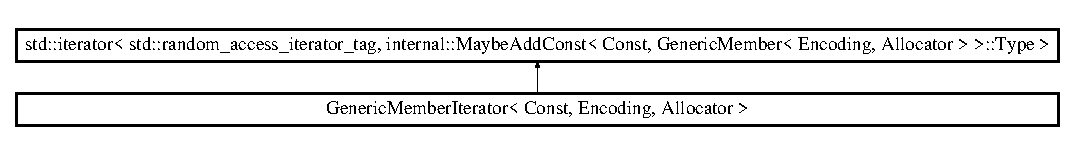
\includegraphics[height=1.462141cm]{a02004}
\end{center}
\end{figure}
\subsection*{Public Types}
\begin{DoxyCompactItemize}
\item 
\mbox{\Hypertarget{a02004_ad1cf1ecf6210b47906c9f179c893a8b8}\label{a02004_ad1cf1ecf6210b47906c9f179c893a8b8}} 
typedef \hyperlink{a02004}{Generic\+Member\+Iterator} \hyperlink{a02004_ad1cf1ecf6210b47906c9f179c893a8b8}{Iterator}
\begin{DoxyCompactList}\small\item\em Iterator type itself. \end{DoxyCompactList}\item 
\mbox{\Hypertarget{a02004_ae5be27a73dce0be58ee2776db896d591}\label{a02004_ae5be27a73dce0be58ee2776db896d591}} 
typedef \hyperlink{a02004}{Generic\+Member\+Iterator}$<$ true, Encoding, Allocator $>$ \hyperlink{a02004_ae5be27a73dce0be58ee2776db896d591}{Const\+Iterator}
\begin{DoxyCompactList}\small\item\em Constant iterator type. \end{DoxyCompactList}\item 
\mbox{\Hypertarget{a02004_abc26eb06f2962765b11dcd06ce84ac02}\label{a02004_abc26eb06f2962765b11dcd06ce84ac02}} 
typedef \hyperlink{a02004}{Generic\+Member\+Iterator}$<$ false, Encoding, Allocator $>$ \hyperlink{a02004_abc26eb06f2962765b11dcd06ce84ac02}{Non\+Const\+Iterator}
\begin{DoxyCompactList}\small\item\em Non-\/constant iterator type. \end{DoxyCompactList}\item 
\mbox{\Hypertarget{a02004_ac69f141f1fde31c1f550f524a69c5de9}\label{a02004_ac69f141f1fde31c1f550f524a69c5de9}} 
typedef Base\+Type\+::pointer \hyperlink{a02004_ac69f141f1fde31c1f550f524a69c5de9}{Pointer}
\begin{DoxyCompactList}\small\item\em Pointer to (const) \hyperlink{a02000}{Generic\+Member}. \end{DoxyCompactList}\item 
\mbox{\Hypertarget{a02004_ae80f6b601eb9e24f73aa75fb32b35c65}\label{a02004_ae80f6b601eb9e24f73aa75fb32b35c65}} 
typedef Base\+Type\+::reference \hyperlink{a02004_ae80f6b601eb9e24f73aa75fb32b35c65}{Reference}
\begin{DoxyCompactList}\small\item\em Reference to (const) \hyperlink{a02000}{Generic\+Member}. \end{DoxyCompactList}\item 
\mbox{\Hypertarget{a02004_a902b99c8ae351cd7626514dc5f30740a}\label{a02004_a902b99c8ae351cd7626514dc5f30740a}} 
typedef Base\+Type\+::difference\+\_\+type \hyperlink{a02004_a902b99c8ae351cd7626514dc5f30740a}{Difference\+Type}
\begin{DoxyCompactList}\small\item\em Signed integer type (e.\+g. {\ttfamily ptrdiff\+\_\+t}) \end{DoxyCompactList}\end{DoxyCompactItemize}
\subsection*{Public Member Functions}
\begin{DoxyCompactItemize}
\item 
\hyperlink{a02004_a2708717d497a0aadacdf75900de4c5b4}{Generic\+Member\+Iterator} ()
\begin{DoxyCompactList}\small\item\em Default constructor (singular value) \end{DoxyCompactList}\item 
\hyperlink{a02004_a2697fd327a90654b0bf91c988e43f95e}{Generic\+Member\+Iterator} (const \hyperlink{a02004_abc26eb06f2962765b11dcd06ce84ac02}{Non\+Const\+Iterator} \&it)
\begin{DoxyCompactList}\small\item\em Iterator conversions to more const. \end{DoxyCompactList}\item 
\mbox{\Hypertarget{a02004_a4ebb2b80e7d70c11802520ae77958df3}\label{a02004_a4ebb2b80e7d70c11802520ae77958df3}} 
\hyperlink{a02004_ad1cf1ecf6210b47906c9f179c893a8b8}{Iterator} \& {\bfseries operator=} (const \hyperlink{a02004_abc26eb06f2962765b11dcd06ce84ac02}{Non\+Const\+Iterator} \&it)
\item 
\mbox{\Hypertarget{a02004_ae119ae8ed78dbd980f83d367f59a3c94}\label{a02004_ae119ae8ed78dbd980f83d367f59a3c94}} 
\hyperlink{a02004_a902b99c8ae351cd7626514dc5f30740a}{Difference\+Type} \hyperlink{a02004_ae119ae8ed78dbd980f83d367f59a3c94}{operator-\/} (\hyperlink{a02004_ae5be27a73dce0be58ee2776db896d591}{Const\+Iterator} that) const
\begin{DoxyCompactList}\small\item\em Distance. \end{DoxyCompactList}\end{DoxyCompactItemize}
\begin{Indent}\textbf{ stepping}\par
\begin{DoxyCompactItemize}
\item 
\mbox{\Hypertarget{a02004_afd6c9a104e2285d1d0b50bde53c9109e}\label{a02004_afd6c9a104e2285d1d0b50bde53c9109e}} 
\hyperlink{a02004_ad1cf1ecf6210b47906c9f179c893a8b8}{Iterator} \& {\bfseries operator++} ()
\item 
\mbox{\Hypertarget{a02004_a6db8972f02d74b663b6ef90ee3ff34f6}\label{a02004_a6db8972f02d74b663b6ef90ee3ff34f6}} 
\hyperlink{a02004_ad1cf1ecf6210b47906c9f179c893a8b8}{Iterator} \& {\bfseries operator-\/-\/} ()
\item 
\mbox{\Hypertarget{a02004_a83c8be6d960213ce32d68a880a8d9089}\label{a02004_a83c8be6d960213ce32d68a880a8d9089}} 
\hyperlink{a02004_ad1cf1ecf6210b47906c9f179c893a8b8}{Iterator} {\bfseries operator++} (int)
\item 
\mbox{\Hypertarget{a02004_a4606c8baec5ea2b5139a503f7caa5444}\label{a02004_a4606c8baec5ea2b5139a503f7caa5444}} 
\hyperlink{a02004_ad1cf1ecf6210b47906c9f179c893a8b8}{Iterator} {\bfseries operator-\/-\/} (int)
\end{DoxyCompactItemize}
\end{Indent}
\begin{Indent}\textbf{ increment/decrement}\par
\begin{DoxyCompactItemize}
\item 
\mbox{\Hypertarget{a02004_a472098839cec785b43a005a23d7a284b}\label{a02004_a472098839cec785b43a005a23d7a284b}} 
\hyperlink{a02004_ad1cf1ecf6210b47906c9f179c893a8b8}{Iterator} {\bfseries operator+} (\hyperlink{a02004_a902b99c8ae351cd7626514dc5f30740a}{Difference\+Type} n) const
\item 
\mbox{\Hypertarget{a02004_a343099509473934b40b9a4264c472721}\label{a02004_a343099509473934b40b9a4264c472721}} 
\hyperlink{a02004_ad1cf1ecf6210b47906c9f179c893a8b8}{Iterator} {\bfseries operator-\/} (\hyperlink{a02004_a902b99c8ae351cd7626514dc5f30740a}{Difference\+Type} n) const
\item 
\mbox{\Hypertarget{a02004_a1fc75f09d68b0f5d92f18ae8c4133e6a}\label{a02004_a1fc75f09d68b0f5d92f18ae8c4133e6a}} 
\hyperlink{a02004_ad1cf1ecf6210b47906c9f179c893a8b8}{Iterator} \& {\bfseries operator+=} (\hyperlink{a02004_a902b99c8ae351cd7626514dc5f30740a}{Difference\+Type} n)
\item 
\mbox{\Hypertarget{a02004_a7cd0c5f194007ec24fa9fa5c13e2502a}\label{a02004_a7cd0c5f194007ec24fa9fa5c13e2502a}} 
\hyperlink{a02004_ad1cf1ecf6210b47906c9f179c893a8b8}{Iterator} \& {\bfseries operator-\/=} (\hyperlink{a02004_a902b99c8ae351cd7626514dc5f30740a}{Difference\+Type} n)
\end{DoxyCompactItemize}
\end{Indent}
\begin{Indent}\textbf{ relations}\par
\begin{DoxyCompactItemize}
\item 
\mbox{\Hypertarget{a02004_a19a0ae160e627e733e192ad018686e7e}\label{a02004_a19a0ae160e627e733e192ad018686e7e}} 
bool {\bfseries operator==} (\hyperlink{a02004_ae5be27a73dce0be58ee2776db896d591}{Const\+Iterator} that) const
\item 
\mbox{\Hypertarget{a02004_a2b2ccd1220d5bc92eef2fbc8824c9ecf}\label{a02004_a2b2ccd1220d5bc92eef2fbc8824c9ecf}} 
bool {\bfseries operator!=} (\hyperlink{a02004_ae5be27a73dce0be58ee2776db896d591}{Const\+Iterator} that) const
\item 
\mbox{\Hypertarget{a02004_a65c30731f77ed249c53c5cf55c9859e2}\label{a02004_a65c30731f77ed249c53c5cf55c9859e2}} 
bool {\bfseries operator$<$=} (\hyperlink{a02004_ae5be27a73dce0be58ee2776db896d591}{Const\+Iterator} that) const
\item 
\mbox{\Hypertarget{a02004_a7d189ea30820684eec8efa847ed7a295}\label{a02004_a7d189ea30820684eec8efa847ed7a295}} 
bool {\bfseries operator$>$=} (\hyperlink{a02004_ae5be27a73dce0be58ee2776db896d591}{Const\+Iterator} that) const
\item 
\mbox{\Hypertarget{a02004_acacffbbad7fca1ca5da64d3041dd2778}\label{a02004_acacffbbad7fca1ca5da64d3041dd2778}} 
bool {\bfseries operator$<$} (\hyperlink{a02004_ae5be27a73dce0be58ee2776db896d591}{Const\+Iterator} that) const
\item 
\mbox{\Hypertarget{a02004_ae5dd7328fc780a57dd069d2183c9a26d}\label{a02004_ae5dd7328fc780a57dd069d2183c9a26d}} 
bool {\bfseries operator$>$} (\hyperlink{a02004_ae5be27a73dce0be58ee2776db896d591}{Const\+Iterator} that) const
\end{DoxyCompactItemize}
\end{Indent}
\begin{Indent}\textbf{ dereference}\par
\begin{DoxyCompactItemize}
\item 
\mbox{\Hypertarget{a02004_a56ad403f7e7a35d6060931685d6cbbe8}\label{a02004_a56ad403f7e7a35d6060931685d6cbbe8}} 
\hyperlink{a02004_ae80f6b601eb9e24f73aa75fb32b35c65}{Reference} {\bfseries operator$\ast$} () const
\item 
\mbox{\Hypertarget{a02004_abc95a8e52653a8baa2927b03239f4be9}\label{a02004_abc95a8e52653a8baa2927b03239f4be9}} 
\hyperlink{a02004_ac69f141f1fde31c1f550f524a69c5de9}{Pointer} {\bfseries operator-\/$>$} () const
\item 
\mbox{\Hypertarget{a02004_a41b59f1bd367a98ee5d1138cc81e98a7}\label{a02004_a41b59f1bd367a98ee5d1138cc81e98a7}} 
\hyperlink{a02004_ae80f6b601eb9e24f73aa75fb32b35c65}{Reference} {\bfseries operator\mbox{[}$\,$\mbox{]}} (\hyperlink{a02004_a902b99c8ae351cd7626514dc5f30740a}{Difference\+Type} n) const
\end{DoxyCompactItemize}
\end{Indent}
\subsection*{Friends}
\begin{DoxyCompactItemize}
\item 
\mbox{\Hypertarget{a02004_a82bdd5798f1a5ac0e3e7ba4bd6938cfc}\label{a02004_a82bdd5798f1a5ac0e3e7ba4bd6938cfc}} 
class {\bfseries Generic\+Value$<$ Encoding, Allocator $>$}
\item 
\mbox{\Hypertarget{a02004_aa375aeb1ffac85cddc3a72a6c24ec6e1}\label{a02004_aa375aeb1ffac85cddc3a72a6c24ec6e1}} 
{\footnotesize template$<$bool , typename , typename $>$ }\\class {\bfseries Generic\+Member\+Iterator}
\end{DoxyCompactItemize}


\subsection{Detailed Description}
\subsubsection*{template$<$bool Const, typename Encoding, typename Allocator$>$\newline
class Generic\+Member\+Iterator$<$ Const, Encoding, Allocator $>$}

(Constant) member iterator for a J\+S\+ON object value 


\begin{DoxyTemplParams}{Template Parameters}
{\em Const} & Is this a constant iterator? \\
\hline
{\em Encoding} & Encoding of the value. (Even non-\/string values need to have the same encoding in a document) \\
\hline
{\em Allocator} & Allocator type for allocating memory of object, array and string.\\
\hline
\end{DoxyTemplParams}
This class implements a Random Access Iterator for \hyperlink{a02000}{Generic\+Member} elements of a \hyperlink{a01992}{Generic\+Value}, see I\+S\+O/\+I\+EC 14882\+:2003(E) C++ standard, 24.\+1 \mbox{[}lib.\+iterator.\+requirements\mbox{]}.

\begin{DoxyNote}{Note}
This iterator implementation is mainly intended to avoid implicit conversions from iterator values to {\ttfamily N\+U\+LL}, e.\+g. from Generic\+Value\+::\+Find\+Member.

Define {\ttfamily R\+A\+P\+I\+D\+J\+S\+O\+N\+\_\+\+N\+O\+M\+E\+M\+B\+E\+R\+I\+T\+E\+R\+A\+T\+O\+R\+C\+L\+A\+SS} to fall back to a pointer-\/based implementation, if your platform doesn\textquotesingle{}t provide the C++ $<$iterator$>$ header.
\end{DoxyNote}
\begin{DoxySeeAlso}{See also}
\hyperlink{a02000}{Generic\+Member}, \hyperlink{a01992_a349b8faae61edc42b4289726820be439}{Generic\+Value\+::\+Member\+Iterator}, \hyperlink{a01992_aac08c3e660a9036d3dcb8b10ff6c61f4}{Generic\+Value\+::\+Const\+Member\+Iterator} 
\end{DoxySeeAlso}


\subsection{Constructor \& Destructor Documentation}
\mbox{\Hypertarget{a02004_a2708717d497a0aadacdf75900de4c5b4}\label{a02004_a2708717d497a0aadacdf75900de4c5b4}} 
\index{Generic\+Member\+Iterator@{Generic\+Member\+Iterator}!Generic\+Member\+Iterator@{Generic\+Member\+Iterator}}
\index{Generic\+Member\+Iterator@{Generic\+Member\+Iterator}!Generic\+Member\+Iterator@{Generic\+Member\+Iterator}}
\subsubsection{\texorpdfstring{Generic\+Member\+Iterator()}{GenericMemberIterator()}\hspace{0.1cm}{\footnotesize\ttfamily [1/2]}}
{\footnotesize\ttfamily template$<$bool Const, typename Encoding , typename Allocator $>$ \\
\hyperlink{a02004}{Generic\+Member\+Iterator}$<$ Const, Encoding, Allocator $>$\+::\hyperlink{a02004}{Generic\+Member\+Iterator} (\begin{DoxyParamCaption}{ }\end{DoxyParamCaption})\hspace{0.3cm}{\ttfamily [inline]}}



Default constructor (singular value) 

Creates an iterator pointing to no element. \begin{DoxyNote}{Note}
All operations, except for comparisons, are undefined on such values. 
\end{DoxyNote}
\mbox{\Hypertarget{a02004_a2697fd327a90654b0bf91c988e43f95e}\label{a02004_a2697fd327a90654b0bf91c988e43f95e}} 
\index{Generic\+Member\+Iterator@{Generic\+Member\+Iterator}!Generic\+Member\+Iterator@{Generic\+Member\+Iterator}}
\index{Generic\+Member\+Iterator@{Generic\+Member\+Iterator}!Generic\+Member\+Iterator@{Generic\+Member\+Iterator}}
\subsubsection{\texorpdfstring{Generic\+Member\+Iterator()}{GenericMemberIterator()}\hspace{0.1cm}{\footnotesize\ttfamily [2/2]}}
{\footnotesize\ttfamily template$<$bool Const, typename Encoding , typename Allocator $>$ \\
\hyperlink{a02004}{Generic\+Member\+Iterator}$<$ Const, Encoding, Allocator $>$\+::\hyperlink{a02004}{Generic\+Member\+Iterator} (\begin{DoxyParamCaption}\item[{const \hyperlink{a02004_abc26eb06f2962765b11dcd06ce84ac02}{Non\+Const\+Iterator} \&}]{it }\end{DoxyParamCaption})\hspace{0.3cm}{\ttfamily [inline]}}



Iterator conversions to more const. 


\begin{DoxyParams}{Parameters}
{\em it} & (Non-\/const) iterator to copy from\\
\hline
\end{DoxyParams}
Allows the creation of an iterator from another \hyperlink{a02004}{Generic\+Member\+Iterator} that is \char`\"{}less const\char`\"{}. Especially, creating a non-\/constant iterator from a constant iterator are disabled\+: \begin{DoxyItemize}
\item const -\/$>$ non-\/const (not ok) \item const -\/$>$ const (ok) \item non-\/const -\/$>$ const (ok) \item non-\/const -\/$>$ non-\/const (ok)\end{DoxyItemize}
\begin{DoxyNote}{Note}
If the {\ttfamily Const} template parameter is already {\ttfamily false}, this constructor effectively defines a regular copy-\/constructor. Otherwise, the copy constructor is implicitly defined. 
\end{DoxyNote}


The documentation for this class was generated from the following file\+:\begin{DoxyCompactItemize}
\item 
\hyperlink{a00476}{document.\+h}\end{DoxyCompactItemize}

\hypertarget{a02212}{}\section{Generic\+Memory\+Buffer$<$ Allocator $>$ Struct Template Reference}
\label{a02212}\index{Generic\+Memory\+Buffer$<$ Allocator $>$@{Generic\+Memory\+Buffer$<$ Allocator $>$}}


Represents an in-\/memory output byte stream.  




{\ttfamily \#include $<$memorybuffer.\+h$>$}

\subsection*{Public Types}
\begin{DoxyCompactItemize}
\item 
\mbox{\Hypertarget{a02212_a212f137abfd8bce2ad216b2d960c027f}\label{a02212_a212f137abfd8bce2ad216b2d960c027f}} 
typedef char {\bfseries Ch}
\end{DoxyCompactItemize}
\subsection*{Public Member Functions}
\begin{DoxyCompactItemize}
\item 
\mbox{\Hypertarget{a02212_ad08f7da47bca43fcdb0c3b10e22dfa1d}\label{a02212_ad08f7da47bca43fcdb0c3b10e22dfa1d}} 
{\bfseries Generic\+Memory\+Buffer} (Allocator $\ast$allocator=0, size\+\_\+t capacity=k\+Default\+Capacity)
\item 
\mbox{\Hypertarget{a02212_a9dfb477983e211893601f8ab637b42d8}\label{a02212_a9dfb477983e211893601f8ab637b42d8}} 
void {\bfseries Put} (Ch c)
\item 
\mbox{\Hypertarget{a02212_a9861181cab6f5bec2ec08b601aa53575}\label{a02212_a9861181cab6f5bec2ec08b601aa53575}} 
void {\bfseries Flush} ()
\item 
\mbox{\Hypertarget{a02212_a036cbe2556778e1edc525602a9821df2}\label{a02212_a036cbe2556778e1edc525602a9821df2}} 
void {\bfseries Clear} ()
\item 
\mbox{\Hypertarget{a02212_a3b87deb9bf34c394c8fb262ab53c0c4b}\label{a02212_a3b87deb9bf34c394c8fb262ab53c0c4b}} 
void {\bfseries Shrink\+To\+Fit} ()
\item 
\mbox{\Hypertarget{a02212_a56f7b14d2940b682fe592f598d6792ec}\label{a02212_a56f7b14d2940b682fe592f598d6792ec}} 
Ch $\ast$ {\bfseries Push} (size\+\_\+t count)
\item 
\mbox{\Hypertarget{a02212_a82a6706286f1356e1769282f5d496005}\label{a02212_a82a6706286f1356e1769282f5d496005}} 
void {\bfseries Pop} (size\+\_\+t count)
\item 
\mbox{\Hypertarget{a02212_a8d7be8b1d64285b787571541a7c4bb37}\label{a02212_a8d7be8b1d64285b787571541a7c4bb37}} 
const Ch $\ast$ {\bfseries Get\+Buffer} () const
\item 
\mbox{\Hypertarget{a02212_aaab1f18d03109ab01213d3e3d8368ff9}\label{a02212_aaab1f18d03109ab01213d3e3d8368ff9}} 
size\+\_\+t {\bfseries Get\+Size} () const
\end{DoxyCompactItemize}
\subsection*{Public Attributes}
\begin{DoxyCompactItemize}
\item 
\mbox{\Hypertarget{a02212_a977b479180bebe8ae14ca1c11d52a486}\label{a02212_a977b479180bebe8ae14ca1c11d52a486}} 
\hyperlink{a02288}{internal\+::\+Stack}$<$ Allocator $>$ {\bfseries stack\+\_\+}
\end{DoxyCompactItemize}
\subsection*{Static Public Attributes}
\begin{DoxyCompactItemize}
\item 
\mbox{\Hypertarget{a02212_af6ecdbdbb8d3aa53cdef6e788e4980be}\label{a02212_af6ecdbdbb8d3aa53cdef6e788e4980be}} 
static const size\+\_\+t {\bfseries k\+Default\+Capacity} = 256
\end{DoxyCompactItemize}


\subsection{Detailed Description}
\subsubsection*{template$<$typename Allocator = Crt\+Allocator$>$\newline
struct Generic\+Memory\+Buffer$<$ Allocator $>$}

Represents an in-\/memory output byte stream. 

This class is mainly for being wrapped by \hyperlink{a02132}{Encoded\+Output\+Stream} or \hyperlink{a02140}{Auto\+U\+T\+F\+Output\+Stream}.

It is similar to File\+Write\+Buffer but the destination is an in-\/memory buffer instead of a file.

Differences between Memory\+Buffer and String\+Buffer\+:
\begin{DoxyEnumerate}
\item String\+Buffer has Encoding but Memory\+Buffer is only a byte buffer.
\item String\+Buffer\+::\+Get\+String() returns a null-\/terminated string. Memory\+Buffer\+::\+Get\+Buffer() returns a buffer without terminator.
\end{DoxyEnumerate}


\begin{DoxyTemplParams}{Template Parameters}
{\em Allocator} & type for allocating memory buffer. \\
\hline
\end{DoxyTemplParams}
\begin{DoxyNote}{Note}
implements Stream concept 
\end{DoxyNote}


The documentation for this struct was generated from the following files\+:\begin{DoxyCompactItemize}
\item 
fwd.\+h\item 
memorybuffer.\+h\end{DoxyCompactItemize}

\hypertarget{a02080}{}\section{Generic\+Object$<$ Const, ValueT $>$ Class Template Reference}
\label{a02080}\index{Generic\+Object$<$ Const, Value\+T $>$@{Generic\+Object$<$ Const, Value\+T $>$}}


Helper class for accessing Value of object type.  




{\ttfamily \#include $<$document.\+h$>$}

\subsection*{Public Types}
\begin{DoxyCompactItemize}
\item 
\mbox{\Hypertarget{a02080_aeee588f9a85e88cac89b7c4dfb6b0bd3}\label{a02080_aeee588f9a85e88cac89b7c4dfb6b0bd3}} 
typedef \hyperlink{a02080}{Generic\+Object}$<$ true, ValueT $>$ {\bfseries Const\+Object}
\item 
\mbox{\Hypertarget{a02080_ae8f5673d0cf8e7ebfd2d4f6ab27b632d}\label{a02080_ae8f5673d0cf8e7ebfd2d4f6ab27b632d}} 
typedef \hyperlink{a02080}{Generic\+Object}$<$ false, ValueT $>$ {\bfseries Object}
\item 
\mbox{\Hypertarget{a02080_a4c25f4a5f696745c418b91ad9f577f12}\label{a02080_a4c25f4a5f696745c418b91ad9f577f12}} 
typedef ValueT {\bfseries Plain\+Type}
\item 
\mbox{\Hypertarget{a02080_a930aa30f89caee7ba7bff60bf9dc21b1}\label{a02080_a930aa30f89caee7ba7bff60bf9dc21b1}} 
typedef internal\+::\+Maybe\+Add\+Const$<$ Const, Plain\+Type $>$\+::\hyperlink{a00560_a1d1cfd8ffb84e947f82999c682b666a7}{Type} {\bfseries Value\+Type}
\item 
\mbox{\Hypertarget{a02080_a1f531d70f8d57ed30199ac445b5935e6}\label{a02080_a1f531d70f8d57ed30199ac445b5935e6}} 
typedef \hyperlink{a02004}{Generic\+Member\+Iterator}$<$ Const, typename Value\+T\+::\+Encoding\+Type, typename Value\+T\+::\+Allocator\+Type $>$ {\bfseries Member\+Iterator}
\item 
\mbox{\Hypertarget{a02080_af16706c0ad32b957c56e7d0541628cd5}\label{a02080_af16706c0ad32b957c56e7d0541628cd5}} 
typedef \hyperlink{a02004}{Generic\+Member\+Iterator}$<$ true, typename Value\+T\+::\+Encoding\+Type, typename Value\+T\+::\+Allocator\+Type $>$ {\bfseries Const\+Member\+Iterator}
\item 
\mbox{\Hypertarget{a02080_a00c8cee952d5ebadc5e1c309aa489ad9}\label{a02080_a00c8cee952d5ebadc5e1c309aa489ad9}} 
typedef Value\+Type\+::\+Allocator\+Type {\bfseries Allocator\+Type}
\item 
\mbox{\Hypertarget{a02080_a9b8381fc96f5f89b2163b052ed66cc59}\label{a02080_a9b8381fc96f5f89b2163b052ed66cc59}} 
typedef Value\+Type\+::\+String\+Ref\+Type {\bfseries String\+Ref\+Type}
\item 
\mbox{\Hypertarget{a02080_a96ebfdde095e2ce42535d15ae5dc58ef}\label{a02080_a96ebfdde095e2ce42535d15ae5dc58ef}} 
typedef Value\+Type\+::\+Encoding\+Type {\bfseries Encoding\+Type}
\item 
\mbox{\Hypertarget{a02080_ac6747e5baa13e15bcea1658b5624647a}\label{a02080_ac6747e5baa13e15bcea1658b5624647a}} 
typedef Value\+Type\+::\+Ch {\bfseries Ch}
\end{DoxyCompactItemize}
\subsection*{Public Member Functions}
\begin{DoxyCompactItemize}
\item 
\mbox{\Hypertarget{a02080_a10173c42d0e8a71ca0e3ae75d800887a}\label{a02080_a10173c42d0e8a71ca0e3ae75d800887a}} 
{\bfseries Generic\+Object} (const \hyperlink{a02080}{Generic\+Object} \&rhs)
\item 
\mbox{\Hypertarget{a02080_af8984f76d6f3b13039c6d3b8e217f747}\label{a02080_af8984f76d6f3b13039c6d3b8e217f747}} 
\hyperlink{a02080}{Generic\+Object} \& {\bfseries operator=} (const \hyperlink{a02080}{Generic\+Object} \&rhs)
\item 
\mbox{\Hypertarget{a02080_a15326564c82f2b545811f753534563e4}\label{a02080_a15326564c82f2b545811f753534563e4}} 
\hyperlink{a00560_a5ed6e6e67250fadbd041127e6386dcb5}{Size\+Type} {\bfseries Member\+Count} () const
\item 
\mbox{\Hypertarget{a02080_a9cc10bfeeb6a5eb95ba1ae587b6e6ad8}\label{a02080_a9cc10bfeeb6a5eb95ba1ae587b6e6ad8}} 
bool {\bfseries Object\+Empty} () const
\item 
\mbox{\Hypertarget{a02080_a2d8c758d10e7c7ab23e3904d5936b204}\label{a02080_a2d8c758d10e7c7ab23e3904d5936b204}} 
{\footnotesize template$<$typename T $>$ }\\Value\+Type \& {\bfseries operator\mbox{[}$\,$\mbox{]}} (T $\ast$name) const
\item 
\mbox{\Hypertarget{a02080_a19bfc1bd98b120d42e7d50db0886614a}\label{a02080_a19bfc1bd98b120d42e7d50db0886614a}} 
{\footnotesize template$<$typename Source\+Allocator $>$ }\\Value\+Type \& {\bfseries operator\mbox{[}$\,$\mbox{]}} (const \hyperlink{a01992}{Generic\+Value}$<$ Encoding\+Type, Source\+Allocator $>$ \&name) const
\item 
\mbox{\Hypertarget{a02080_af1e80a8a521f05530f9b6a448242ff2d}\label{a02080_af1e80a8a521f05530f9b6a448242ff2d}} 
\hyperlink{a02004}{Member\+Iterator} {\bfseries Member\+Begin} () const
\item 
\mbox{\Hypertarget{a02080_a75873786614f67796bfb190008e004dc}\label{a02080_a75873786614f67796bfb190008e004dc}} 
\hyperlink{a02004}{Member\+Iterator} {\bfseries Member\+End} () const
\item 
\mbox{\Hypertarget{a02080_a996d775e52cc7c5cf2aa308cf5a2b2cf}\label{a02080_a996d775e52cc7c5cf2aa308cf5a2b2cf}} 
bool {\bfseries Has\+Member} (const Ch $\ast$name) const
\item 
\mbox{\Hypertarget{a02080_a0b63666ca05c86f9d719350f2302a3f7}\label{a02080_a0b63666ca05c86f9d719350f2302a3f7}} 
{\footnotesize template$<$typename Source\+Allocator $>$ }\\bool {\bfseries Has\+Member} (const \hyperlink{a01992}{Generic\+Value}$<$ Encoding\+Type, Source\+Allocator $>$ \&name) const
\item 
\mbox{\Hypertarget{a02080_a979890ccb3b116af19f9e3e77d3d286f}\label{a02080_a979890ccb3b116af19f9e3e77d3d286f}} 
\hyperlink{a02004}{Member\+Iterator} {\bfseries Find\+Member} (const Ch $\ast$name) const
\item 
\mbox{\Hypertarget{a02080_a12a4fbbf2219d6bb43c3d61923830ab4}\label{a02080_a12a4fbbf2219d6bb43c3d61923830ab4}} 
{\footnotesize template$<$typename Source\+Allocator $>$ }\\\hyperlink{a02004}{Member\+Iterator} {\bfseries Find\+Member} (const \hyperlink{a01992}{Generic\+Value}$<$ Encoding\+Type, Source\+Allocator $>$ \&name) const
\item 
\mbox{\Hypertarget{a02080_a3668524c8566c46cbae97d938064f5fa}\label{a02080_a3668524c8566c46cbae97d938064f5fa}} 
\hyperlink{a02080}{Generic\+Object} {\bfseries Add\+Member} (Value\+Type \&name, Value\+Type \&value, Allocator\+Type \&allocator) const
\item 
\mbox{\Hypertarget{a02080_ae871adc8c906a72878b7cf5df279ed1f}\label{a02080_ae871adc8c906a72878b7cf5df279ed1f}} 
\hyperlink{a02080}{Generic\+Object} {\bfseries Add\+Member} (Value\+Type \&name, String\+Ref\+Type value, Allocator\+Type \&allocator) const
\item 
\mbox{\Hypertarget{a02080_a98ebcec632c41442d89cd8634b7ecc47}\label{a02080_a98ebcec632c41442d89cd8634b7ecc47}} 
{\footnotesize template$<$typename T $>$ }\\{\bfseries R\+A\+P\+I\+D\+J\+S\+O\+N\+\_\+\+D\+I\+S\+A\+B\+L\+E\+I\+F\+\_\+\+R\+E\+T\+U\+RN} ((internal\+::\+Or\+Expr$<$ internal\+::\+Is\+Pointer$<$ T $>$, \hyperlink{a02020}{internal\+::\+Is\+Generic\+Value}$<$ T $>$ $>$),(Value\+Type \&)) Add\+Member(Value\+Type \&name
\item 
\mbox{\Hypertarget{a02080_a011a0dd06baf841e3f6e21a3c95db3c1}\label{a02080_a011a0dd06baf841e3f6e21a3c95db3c1}} 
\hyperlink{a02080}{Generic\+Object} {\bfseries Add\+Member} (String\+Ref\+Type name, Value\+Type \&value, Allocator\+Type \&allocator) const
\item 
\mbox{\Hypertarget{a02080_a3af43681aea03c4313d689bcbf5e3363}\label{a02080_a3af43681aea03c4313d689bcbf5e3363}} 
\hyperlink{a02080}{Generic\+Object} {\bfseries Add\+Member} (String\+Ref\+Type name, String\+Ref\+Type value, Allocator\+Type \&allocator) const
\item 
\mbox{\Hypertarget{a02080_af361a4b677882964789201fc605541d0}\label{a02080_af361a4b677882964789201fc605541d0}} 
{\footnotesize template$<$typename T $>$ }\\{\bfseries R\+A\+P\+I\+D\+J\+S\+O\+N\+\_\+\+D\+I\+S\+A\+B\+L\+E\+I\+F\+\_\+\+R\+E\+T\+U\+RN} ((internal\+::\+Or\+Expr$<$ internal\+::\+Is\+Pointer$<$ T $>$, \hyperlink{a02020}{internal\+::\+Is\+Generic\+Value}$<$ T $>$ $>$),(\hyperlink{a02080}{Generic\+Object})) Add\+Member(String\+Ref\+Type name
\item 
\mbox{\Hypertarget{a02080_a129ce3843a6658e620a7f740d9f44ee1}\label{a02080_a129ce3843a6658e620a7f740d9f44ee1}} 
void {\bfseries Remove\+All\+Members} ()
\item 
\mbox{\Hypertarget{a02080_aebeda9c2cac6afd56dda55caaf2c4a0c}\label{a02080_aebeda9c2cac6afd56dda55caaf2c4a0c}} 
bool {\bfseries Remove\+Member} (const Ch $\ast$name) const
\item 
\mbox{\Hypertarget{a02080_a8e29dc07b992e71e35dd93a57f95842c}\label{a02080_a8e29dc07b992e71e35dd93a57f95842c}} 
{\footnotesize template$<$typename Source\+Allocator $>$ }\\bool {\bfseries Remove\+Member} (const \hyperlink{a01992}{Generic\+Value}$<$ Encoding\+Type, Source\+Allocator $>$ \&name) const
\item 
\mbox{\Hypertarget{a02080_a006f76a33dada85c9d13e069cc43623d}\label{a02080_a006f76a33dada85c9d13e069cc43623d}} 
\hyperlink{a02004}{Member\+Iterator} {\bfseries Remove\+Member} (\hyperlink{a02004}{Member\+Iterator} m) const
\item 
\mbox{\Hypertarget{a02080_a29ad0490a4a088d57df7a9884f979a82}\label{a02080_a29ad0490a4a088d57df7a9884f979a82}} 
\hyperlink{a02004}{Member\+Iterator} {\bfseries Erase\+Member} (\hyperlink{a02004}{Const\+Member\+Iterator} pos) const
\item 
\mbox{\Hypertarget{a02080_a67f85d2da462287dead8e35f2ac974b5}\label{a02080_a67f85d2da462287dead8e35f2ac974b5}} 
\hyperlink{a02004}{Member\+Iterator} {\bfseries Erase\+Member} (\hyperlink{a02004}{Const\+Member\+Iterator} first, \hyperlink{a02004}{Const\+Member\+Iterator} last) const
\item 
\mbox{\Hypertarget{a02080_af0d31a8547051624449494a339b20107}\label{a02080_af0d31a8547051624449494a339b20107}} 
bool {\bfseries Erase\+Member} (const Ch $\ast$name) const
\item 
\mbox{\Hypertarget{a02080_a4cd6f90444f20cc9d5577747d3968da4}\label{a02080_a4cd6f90444f20cc9d5577747d3968da4}} 
{\footnotesize template$<$typename Source\+Allocator $>$ }\\bool {\bfseries Erase\+Member} (const \hyperlink{a01992}{Generic\+Value}$<$ Encoding\+Type, Source\+Allocator $>$ \&name) const
\end{DoxyCompactItemize}
\subsection*{Public Attributes}
\begin{DoxyCompactItemize}
\item 
\mbox{\Hypertarget{a02080_a131538fbbacbc0a3a5ad15dbea66394f}\label{a02080_a131538fbbacbc0a3a5ad15dbea66394f}} 
T {\bfseries value}
\item 
\mbox{\Hypertarget{a02080_af70c9646b5e422306c33e98b3d8783a7}\label{a02080_af70c9646b5e422306c33e98b3d8783a7}} 
T Allocator\+Type \&allocator {\bfseries const} \{ value\+\_\+.\+Add\+Member(name, value, allocator)
\item 
\mbox{\Hypertarget{a02080_a719a0e5501da825e6f86ce12b46446cb}\label{a02080_a719a0e5501da825e6f86ce12b46446cb}} 
return $\ast$ {\bfseries this}
\end{DoxyCompactItemize}
\subsection*{Friends}
\begin{DoxyCompactItemize}
\item 
\mbox{\Hypertarget{a02080_a899449e1a645b5e377af059fb61113d8}\label{a02080_a899449e1a645b5e377af059fb61113d8}} 
{\footnotesize template$<$typename , typename $>$ }\\class {\bfseries Generic\+Value}
\end{DoxyCompactItemize}


\subsection{Detailed Description}
\subsubsection*{template$<$bool Const, typename ValueT$>$\newline
class Generic\+Object$<$ Const, Value\+T $>$}

Helper class for accessing Value of object type. 

Instance of this helper class is obtained by {\ttfamily Generic\+Value\+::\+Get\+Object()}. In addition to all A\+P\+Is for array type, it provides range-\/based for loop if {\ttfamily R\+A\+P\+I\+D\+J\+S\+O\+N\+\_\+\+H\+A\+S\+\_\+\+C\+X\+X11\+\_\+\+R\+A\+N\+G\+E\+\_\+\+F\+OR=1}. 

The documentation for this class was generated from the following file\+:\begin{DoxyCompactItemize}
\item 
\hyperlink{a00476}{document.\+h}\end{DoxyCompactItemize}

\hypertarget{a02232}{}\section{Generic\+Pointer$<$ Value\+Type, Allocator $>$ Class Template Reference}
\label{a02232}\index{Generic\+Pointer$<$ Value\+Type, Allocator $>$@{Generic\+Pointer$<$ Value\+Type, Allocator $>$}}


Represents a J\+S\+ON Pointer. Use Pointer for \hyperlink{a02144}{U\+T\+F8} encoding and default allocator.  




{\ttfamily \#include $<$pointer.\+h$>$}

\subsection*{Classes}
\begin{DoxyCompactItemize}
\item 
struct \hyperlink{a02308}{Token}
\begin{DoxyCompactList}\small\item\em A token is the basic units of internal representation. \end{DoxyCompactList}\end{DoxyCompactItemize}
\subsection*{Public Types}
\begin{DoxyCompactItemize}
\item 
\mbox{\Hypertarget{a02232_a4b802da797a7a0b615fd9611cedb7c3b}\label{a02232_a4b802da797a7a0b615fd9611cedb7c3b}} 
typedef Value\+Type\+::\+Encoding\+Type \hyperlink{a02232_a4b802da797a7a0b615fd9611cedb7c3b}{Encoding\+Type}
\begin{DoxyCompactList}\small\item\em Encoding type from Value. \end{DoxyCompactList}\item 
\mbox{\Hypertarget{a02232_ab292356c11b4015c98d21b966b11f285}\label{a02232_ab292356c11b4015c98d21b966b11f285}} 
typedef Value\+Type\+::\+Ch \hyperlink{a02232_ab292356c11b4015c98d21b966b11f285}{Ch}
\begin{DoxyCompactList}\small\item\em Character type from Value. \end{DoxyCompactList}\end{DoxyCompactItemize}
\subsection*{Public Member Functions}
\begin{DoxyCompactItemize}
\item 
\mbox{\Hypertarget{a02232_aebf325c6fde06adfc4d959b507d7f170}\label{a02232_aebf325c6fde06adfc4d959b507d7f170}} 
Allocator stack\+Allocator {\bfseries R\+A\+P\+I\+D\+J\+S\+O\+N\+\_\+\+D\+I\+S\+A\+B\+L\+E\+I\+F\+\_\+\+R\+E\+T\+U\+RN} ((internal\+::\+Or\+Expr$<$ internal\+::\+Is\+Pointer$<$ T $>$, \hyperlink{a02020}{internal\+::\+Is\+Generic\+Value}$<$ T $>$ $>$),(Value\+Type \&)) Get\+With\+Default(\hyperlink{a01996}{Generic\+Document}$<$ \hyperlink{a02232_a4b802da797a7a0b615fd9611cedb7c3b}{Encoding\+Type}
\item 
bool \hyperlink{a02232_a759c07e81c9738e7a2a68b36d5c28643}{Erase} (Value\+Type \&root) const
\begin{DoxyCompactList}\small\item\em Erase a value in a subtree. \end{DoxyCompactList}\end{DoxyCompactItemize}
\begin{Indent}\textbf{ Constructors and destructor.}\par
\begin{DoxyCompactItemize}
\item 
\mbox{\Hypertarget{a02232_a5d85b7dc82719643e8f7adccd5a74fbe}\label{a02232_a5d85b7dc82719643e8f7adccd5a74fbe}} 
\hyperlink{a02232_a5d85b7dc82719643e8f7adccd5a74fbe}{Generic\+Pointer} (Allocator $\ast$allocator=0)
\begin{DoxyCompactList}\small\item\em Default constructor. \end{DoxyCompactList}\item 
\hyperlink{a02232_a4ad549b8a826c3c2dedf03fcc07be9b0}{Generic\+Pointer} (const \hyperlink{a02232_ab292356c11b4015c98d21b966b11f285}{Ch} $\ast$source, Allocator $\ast$allocator=0)
\begin{DoxyCompactList}\small\item\em Constructor that parses a string or U\+RI fragment representation. \end{DoxyCompactList}\item 
\hyperlink{a02232_a9c05684ea95306aac7626e70cb3946cc}{Generic\+Pointer} (const \hyperlink{a02232_ab292356c11b4015c98d21b966b11f285}{Ch} $\ast$source, size\+\_\+t length, Allocator $\ast$allocator=0)
\begin{DoxyCompactList}\small\item\em Constructor that parses a string or U\+RI fragment representation, with length of the source string. \end{DoxyCompactList}\item 
\hyperlink{a02232_a524a9921eff68f389a817a20ca7f1d84}{Generic\+Pointer} (const \hyperlink{a02308}{Token} $\ast$tokens, size\+\_\+t token\+Count)
\begin{DoxyCompactList}\small\item\em Constructor with user-\/supplied tokens. \end{DoxyCompactList}\item 
\mbox{\Hypertarget{a02232_a18d671bb793c6b843d5496b2b130cb70}\label{a02232_a18d671bb793c6b843d5496b2b130cb70}} 
\hyperlink{a02232_a18d671bb793c6b843d5496b2b130cb70}{Generic\+Pointer} (const \hyperlink{a02232}{Generic\+Pointer} \&rhs, Allocator $\ast$allocator=0)
\begin{DoxyCompactList}\small\item\em Copy constructor. \end{DoxyCompactList}\item 
\mbox{\Hypertarget{a02232_acf3eb2f7c4ebf9256f638aafa17534cb}\label{a02232_acf3eb2f7c4ebf9256f638aafa17534cb}} 
\hyperlink{a02232_acf3eb2f7c4ebf9256f638aafa17534cb}{$\sim$\+Generic\+Pointer} ()
\begin{DoxyCompactList}\small\item\em Destructor. \end{DoxyCompactList}\item 
\mbox{\Hypertarget{a02232_a1d0174a6e72daa4024da9e08ce1e7951}\label{a02232_a1d0174a6e72daa4024da9e08ce1e7951}} 
\hyperlink{a02232}{Generic\+Pointer} \& \hyperlink{a02232_a1d0174a6e72daa4024da9e08ce1e7951}{operator=} (const \hyperlink{a02232}{Generic\+Pointer} \&rhs)
\begin{DoxyCompactList}\small\item\em Assignment operator. \end{DoxyCompactList}\end{DoxyCompactItemize}
\end{Indent}
\begin{Indent}\textbf{ Append token}\par
\begin{DoxyCompactItemize}
\item 
\hyperlink{a02232}{Generic\+Pointer} \hyperlink{a02232_aa8f86c0f330807f337351a95ae254b78}{Append} (const \hyperlink{a02308}{Token} \&token, Allocator $\ast$allocator=0) const
\begin{DoxyCompactList}\small\item\em Append a token and return a new Pointer. \end{DoxyCompactList}\item 
\hyperlink{a02232}{Generic\+Pointer} \hyperlink{a02232_a9f8a1711f5b8e0d951c25c6c65326f77}{Append} (const \hyperlink{a02232_ab292356c11b4015c98d21b966b11f285}{Ch} $\ast$name, \hyperlink{a00560_a5ed6e6e67250fadbd041127e6386dcb5}{Size\+Type} length, Allocator $\ast$allocator=0) const
\begin{DoxyCompactList}\small\item\em Append a name token with length, and return a new Pointer. \end{DoxyCompactList}\item 
{\footnotesize template$<$typename T $>$ }\\\hyperlink{a02232_aaf4d7d852098878d24188d134182d42f}{R\+A\+P\+I\+D\+J\+S\+O\+N\+\_\+\+D\+I\+S\+A\+B\+L\+E\+I\+F\+\_\+\+R\+E\+T\+U\+RN} ((internal\+::\+Not\+Expr$<$ internal\+::\+Is\+Same$<$ typename internal\+::\+Remove\+Const$<$ T $>$\+::\hyperlink{a00560_a1d1cfd8ffb84e947f82999c682b666a7}{Type}, \hyperlink{a02232_ab292356c11b4015c98d21b966b11f285}{Ch} $>$ $>$),(\hyperlink{a02232}{Generic\+Pointer})) \hyperlink{a02232_aa8f86c0f330807f337351a95ae254b78}{Append}(T $\ast$name
\begin{DoxyCompactList}\small\item\em Append a name token without length, and return a new Pointer. \end{DoxyCompactList}\end{DoxyCompactItemize}
\end{Indent}
\begin{Indent}\textbf{ Swap a value}\par
\begin{DoxyCompactItemize}
\item 
Value\+Type \& \hyperlink{a02232_a3b40ad3e851640e295a4623b624af395}{Swap} (Value\+Type \&root, Value\+Type \&value, typename Value\+Type\+::\+Allocator\+Type \&allocator) const
\begin{DoxyCompactList}\small\item\em Swap a value with a value in a subtree. \end{DoxyCompactList}\item 
\mbox{\Hypertarget{a02232_aa84bc7e016c906436f464c8cbd858edb}\label{a02232_aa84bc7e016c906436f464c8cbd858edb}} 
{\footnotesize template$<$typename stack\+Allocator $>$ }\\Value\+Type \& \hyperlink{a02232_aa84bc7e016c906436f464c8cbd858edb}{Swap} (\hyperlink{a01996}{Generic\+Document}$<$ \hyperlink{a02232_a4b802da797a7a0b615fd9611cedb7c3b}{Encoding\+Type}, typename Value\+Type\+::\+Allocator\+Type, stack\+Allocator $>$ \&document, Value\+Type \&value) const
\begin{DoxyCompactList}\small\item\em Swap a value with a value in a document. \end{DoxyCompactList}\end{DoxyCompactItemize}
\end{Indent}
\subsection*{Public Attributes}
\begin{DoxyCompactItemize}
\item 
\mbox{\Hypertarget{a02232_aeb61ba8e67260b43090791eeca8b90e0}\label{a02232_aeb61ba8e67260b43090791eeca8b90e0}} 
Allocator $\ast$ {\bfseries allocator}
\item 
\mbox{\Hypertarget{a02232_a646e2825228e0d8331e3a49d7382202b}\label{a02232_a646e2825228e0d8331e3a49d7382202b}} 
Allocator stack\+Allocator stack\+Allocator \& {\bfseries document}
\item 
Allocator stack\+Allocator stack\+Allocator T default\+Value {\bfseries const}
\end{DoxyCompactItemize}
\subsection*{Set a value}
\begin{DoxyCompactItemize}
\item 
\mbox{\Hypertarget{a02232_a08ef35da0ea9a51d8265a360f0c34540}\label{a02232_a08ef35da0ea9a51d8265a360f0c34540}} 
T {\bfseries value}
\item 
T Value\+Type\+::\+Allocator\+Type \&allocator {\bfseries const}
\item 
\mbox{\Hypertarget{a02232_afd073c4e3be53fd7ec08aec9f75fbaa9}\label{a02232_afd073c4e3be53fd7ec08aec9f75fbaa9}} 
stack\+Allocator \& {\bfseries document}
\item 
stack\+Allocator T value {\bfseries const}
\item 
Value\+Type \& \hyperlink{a02232_a71476d125a276b62a246990da1bd3468}{Set} (Value\+Type \&root, Value\+Type \&value, typename Value\+Type\+::\+Allocator\+Type \&allocator) const
\begin{DoxyCompactList}\small\item\em Set a value in a subtree, with move semantics. \end{DoxyCompactList}\item 
\mbox{\Hypertarget{a02232_a61c0e9695cb0c96d465c8e1c21bd48fa}\label{a02232_a61c0e9695cb0c96d465c8e1c21bd48fa}} 
Value\+Type \& \hyperlink{a02232_a61c0e9695cb0c96d465c8e1c21bd48fa}{Set} (Value\+Type \&root, const Value\+Type \&value, typename Value\+Type\+::\+Allocator\+Type \&allocator) const
\begin{DoxyCompactList}\small\item\em Set a value in a subtree, with copy semantics. \end{DoxyCompactList}\item 
\mbox{\Hypertarget{a02232_a37ea2d2b205d3642d1e615b8b866666b}\label{a02232_a37ea2d2b205d3642d1e615b8b866666b}} 
Value\+Type \& \hyperlink{a02232_a37ea2d2b205d3642d1e615b8b866666b}{Set} (Value\+Type \&root, const \hyperlink{a02232_ab292356c11b4015c98d21b966b11f285}{Ch} $\ast$value, typename Value\+Type\+::\+Allocator\+Type \&allocator) const
\begin{DoxyCompactList}\small\item\em Set a null-\/terminated string in a subtree. \end{DoxyCompactList}\item 
{\footnotesize template$<$typename T $>$ }\\\hyperlink{a02232_a914bbdd96e2a248e035b8ebd68526369}{R\+A\+P\+I\+D\+J\+S\+O\+N\+\_\+\+D\+I\+S\+A\+B\+L\+E\+I\+F\+\_\+\+R\+E\+T\+U\+RN} ((internal\+::\+Or\+Expr$<$ internal\+::\+Is\+Pointer$<$ T $>$, \hyperlink{a02020}{internal\+::\+Is\+Generic\+Value}$<$ T $>$ $>$),(Value\+Type \&)) \hyperlink{a02232_a71476d125a276b62a246990da1bd3468}{Set}(Value\+Type \&root
\begin{DoxyCompactList}\small\item\em Set a primitive value in a subtree. \end{DoxyCompactList}\item 
\mbox{\Hypertarget{a02232_aeec3daf051dfa8b8fbf23ea4f9a238e4}\label{a02232_aeec3daf051dfa8b8fbf23ea4f9a238e4}} 
{\footnotesize template$<$typename stack\+Allocator $>$ }\\Value\+Type \& \hyperlink{a02232_aeec3daf051dfa8b8fbf23ea4f9a238e4}{Set} (\hyperlink{a01996}{Generic\+Document}$<$ \hyperlink{a02232_a4b802da797a7a0b615fd9611cedb7c3b}{Encoding\+Type}, typename Value\+Type\+::\+Allocator\+Type, stack\+Allocator $>$ \&document, Value\+Type \&value) const
\begin{DoxyCompactList}\small\item\em Set a value in a document, with move semantics. \end{DoxyCompactList}\item 
\mbox{\Hypertarget{a02232_a8ed0a7ce95331b7433371df7150b84a9}\label{a02232_a8ed0a7ce95331b7433371df7150b84a9}} 
{\footnotesize template$<$typename stack\+Allocator $>$ }\\Value\+Type \& \hyperlink{a02232_a8ed0a7ce95331b7433371df7150b84a9}{Set} (\hyperlink{a01996}{Generic\+Document}$<$ \hyperlink{a02232_a4b802da797a7a0b615fd9611cedb7c3b}{Encoding\+Type}, typename Value\+Type\+::\+Allocator\+Type, stack\+Allocator $>$ \&document, const Value\+Type \&value) const
\begin{DoxyCompactList}\small\item\em Set a value in a document, with copy semantics. \end{DoxyCompactList}\item 
\mbox{\Hypertarget{a02232_abaa0cda4ed84a4435871d355279bab8e}\label{a02232_abaa0cda4ed84a4435871d355279bab8e}} 
{\footnotesize template$<$typename stack\+Allocator $>$ }\\Value\+Type \& \hyperlink{a02232_abaa0cda4ed84a4435871d355279bab8e}{Set} (\hyperlink{a01996}{Generic\+Document}$<$ \hyperlink{a02232_a4b802da797a7a0b615fd9611cedb7c3b}{Encoding\+Type}, typename Value\+Type\+::\+Allocator\+Type, stack\+Allocator $>$ \&document, const \hyperlink{a02232_ab292356c11b4015c98d21b966b11f285}{Ch} $\ast$value) const
\begin{DoxyCompactList}\small\item\em Set a null-\/terminated string in a document. \end{DoxyCompactList}\item 
{\footnotesize template$<$typename T , typename stack\+Allocator $>$ }\\\hyperlink{a02232_a1bb4a253f33687734e5b20795632a801}{R\+A\+P\+I\+D\+J\+S\+O\+N\+\_\+\+D\+I\+S\+A\+B\+L\+E\+I\+F\+\_\+\+R\+E\+T\+U\+RN} ((internal\+::\+Or\+Expr$<$ internal\+::\+Is\+Pointer$<$ T $>$, \hyperlink{a02020}{internal\+::\+Is\+Generic\+Value}$<$ T $>$ $>$),(Value\+Type \&)) \hyperlink{a02232_a71476d125a276b62a246990da1bd3468}{Set}(\hyperlink{a01996}{Generic\+Document}$<$ \hyperlink{a02232_a4b802da797a7a0b615fd9611cedb7c3b}{Encoding\+Type}
\begin{DoxyCompactList}\small\item\em Set a primitive value in a document. \end{DoxyCompactList}\end{DoxyCompactItemize}


\subsection{Detailed Description}
\subsubsection*{template$<$typename Value\+Type, typename Allocator = Crt\+Allocator$>$\newline
class Generic\+Pointer$<$ Value\+Type, Allocator $>$}

Represents a J\+S\+ON Pointer. Use Pointer for \hyperlink{a02144}{U\+T\+F8} encoding and default allocator. 

This class implements R\+FC 6901 \char`\"{}\+Java\+Script Object Notation (\+J\+S\+O\+N) Pointer\char`\"{} (\href{https://tools.ietf.org/html/rfc6901}{\tt https\+://tools.\+ietf.\+org/html/rfc6901}).

A J\+S\+ON pointer is for identifying a specific value in a J\+S\+ON document (\hyperlink{a01996}{Generic\+Document}). It can simplify coding of D\+OM tree manipulation, because it can access multiple-\/level depth of D\+OM tree with single A\+PI call.

After it parses a string representation (e.\+g. \char`\"{}/foo/0\char`\"{} or U\+RI fragment representation (e.\+g. \char`\"{}\#/foo/0\char`\"{}) into its internal representation (tokens), it can be used to resolve a specific value in multiple documents, or sub-\/tree of documents.

Contrary to \hyperlink{a01992}{Generic\+Value}, Pointer can be copy constructed and copy assigned. Apart from assignment, a Pointer cannot be modified after construction.

Although Pointer is very convenient, please aware that constructing Pointer involves parsing and dynamic memory allocation. A special constructor with user-\/ supplied tokens eliminates these.

\hyperlink{a02232}{Generic\+Pointer} depends on \hyperlink{a01996}{Generic\+Document} and \hyperlink{a01992}{Generic\+Value}.


\begin{DoxyTemplParams}{Template Parameters}
{\em Value\+Type} & The value type of the D\+OM tree. E.\+g. \hyperlink{a01992}{Generic\+Value}$<$U\+T\+F8$<$$>$ $>$ \\
\hline
{\em Allocator} & The allocator type for allocating memory for internal representation.\\
\hline
\end{DoxyTemplParams}
\begin{DoxyNote}{Note}
\hyperlink{a02232}{Generic\+Pointer} uses same encoding of Value\+Type. However, Allocator of \hyperlink{a02232}{Generic\+Pointer} is independent of Allocator of Value. 
\end{DoxyNote}


\subsection{Constructor \& Destructor Documentation}
\mbox{\Hypertarget{a02232_a4ad549b8a826c3c2dedf03fcc07be9b0}\label{a02232_a4ad549b8a826c3c2dedf03fcc07be9b0}} 
\index{Generic\+Pointer@{Generic\+Pointer}!Generic\+Pointer@{Generic\+Pointer}}
\index{Generic\+Pointer@{Generic\+Pointer}!Generic\+Pointer@{Generic\+Pointer}}
\subsubsection{\texorpdfstring{Generic\+Pointer()}{GenericPointer()}\hspace{0.1cm}{\footnotesize\ttfamily [1/3]}}
{\footnotesize\ttfamily template$<$typename Value\+Type, typename Allocator = Crt\+Allocator$>$ \\
\hyperlink{a02232}{Generic\+Pointer}$<$ Value\+Type, Allocator $>$\+::\hyperlink{a02232}{Generic\+Pointer} (\begin{DoxyParamCaption}\item[{const \hyperlink{a02232_ab292356c11b4015c98d21b966b11f285}{Ch} $\ast$}]{source,  }\item[{Allocator $\ast$}]{allocator = {\ttfamily 0} }\end{DoxyParamCaption})\hspace{0.3cm}{\ttfamily [inline]}, {\ttfamily [explicit]}}



Constructor that parses a string or U\+RI fragment representation. 


\begin{DoxyParams}{Parameters}
{\em source} & A null-\/terminated, string or U\+RI fragment representation of J\+S\+ON pointer. \\
\hline
{\em allocator} & User supplied allocator for this pointer. If no allocator is provided, it creates a self-\/owned one. \\
\hline
\end{DoxyParams}
\mbox{\Hypertarget{a02232_a9c05684ea95306aac7626e70cb3946cc}\label{a02232_a9c05684ea95306aac7626e70cb3946cc}} 
\index{Generic\+Pointer@{Generic\+Pointer}!Generic\+Pointer@{Generic\+Pointer}}
\index{Generic\+Pointer@{Generic\+Pointer}!Generic\+Pointer@{Generic\+Pointer}}
\subsubsection{\texorpdfstring{Generic\+Pointer()}{GenericPointer()}\hspace{0.1cm}{\footnotesize\ttfamily [2/3]}}
{\footnotesize\ttfamily template$<$typename Value\+Type, typename Allocator = Crt\+Allocator$>$ \\
\hyperlink{a02232}{Generic\+Pointer}$<$ Value\+Type, Allocator $>$\+::\hyperlink{a02232}{Generic\+Pointer} (\begin{DoxyParamCaption}\item[{const \hyperlink{a02232_ab292356c11b4015c98d21b966b11f285}{Ch} $\ast$}]{source,  }\item[{size\+\_\+t}]{length,  }\item[{Allocator $\ast$}]{allocator = {\ttfamily 0} }\end{DoxyParamCaption})\hspace{0.3cm}{\ttfamily [inline]}}



Constructor that parses a string or U\+RI fragment representation, with length of the source string. 


\begin{DoxyParams}{Parameters}
{\em source} & A string or U\+RI fragment representation of J\+S\+ON pointer. \\
\hline
{\em length} & Length of source. \\
\hline
{\em allocator} & User supplied allocator for this pointer. If no allocator is provided, it creates a self-\/owned one. \\
\hline
\end{DoxyParams}
\begin{DoxyNote}{Note}
Slightly faster than the overload without length. 
\end{DoxyNote}
\mbox{\Hypertarget{a02232_a524a9921eff68f389a817a20ca7f1d84}\label{a02232_a524a9921eff68f389a817a20ca7f1d84}} 
\index{Generic\+Pointer@{Generic\+Pointer}!Generic\+Pointer@{Generic\+Pointer}}
\index{Generic\+Pointer@{Generic\+Pointer}!Generic\+Pointer@{Generic\+Pointer}}
\subsubsection{\texorpdfstring{Generic\+Pointer()}{GenericPointer()}\hspace{0.1cm}{\footnotesize\ttfamily [3/3]}}
{\footnotesize\ttfamily template$<$typename Value\+Type, typename Allocator = Crt\+Allocator$>$ \\
\hyperlink{a02232}{Generic\+Pointer}$<$ Value\+Type, Allocator $>$\+::\hyperlink{a02232}{Generic\+Pointer} (\begin{DoxyParamCaption}\item[{const \hyperlink{a02308}{Token} $\ast$}]{tokens,  }\item[{size\+\_\+t}]{token\+Count }\end{DoxyParamCaption})\hspace{0.3cm}{\ttfamily [inline]}}



Constructor with user-\/supplied tokens. 

This constructor let user supplies const array of tokens. This prevents the parsing process and eliminates allocation. This is preferred for memory constrained environments.


\begin{DoxyParams}{Parameters}
{\em tokens} & An constant array of tokens representing the J\+S\+ON pointer. \\
\hline
{\em token\+Count} & Number of tokens.\\
\hline
\end{DoxyParams}
{\bfseries Example} 
\begin{DoxyCode}
\textcolor{preprocessor}{#define NAME(s) \{ s, sizeof(s) / sizeof(s[0]) - 1, kPointerInvalidIndex \}}
\textcolor{preprocessor}{#define INDEX(i) \{ #i, sizeof(#i) - 1, i \}}

\textcolor{keyword}{static} \textcolor{keyword}{const} \hyperlink{a02308}{Pointer::Token} kTokens[] = \{ NAME(\textcolor{stringliteral}{"foo"}), INDEX(123) \};
\textcolor{keyword}{static} \textcolor{keyword}{const} \hyperlink{a02232}{Pointer} p(kTokens, \textcolor{keyword}{sizeof}(kTokens) / \textcolor{keyword}{sizeof}(kTokens[0]));
\textcolor{comment}{// Equivalent to static const Pointer p("/foo/123");}

\textcolor{preprocessor}{#undef NAME}
\textcolor{preprocessor}{#undef INDEX}
\end{DoxyCode}
 

\subsection{Member Function Documentation}
\mbox{\Hypertarget{a02232_aa8f86c0f330807f337351a95ae254b78}\label{a02232_aa8f86c0f330807f337351a95ae254b78}} 
\index{Generic\+Pointer@{Generic\+Pointer}!Append@{Append}}
\index{Append@{Append}!Generic\+Pointer@{Generic\+Pointer}}
\subsubsection{\texorpdfstring{Append()}{Append()}\hspace{0.1cm}{\footnotesize\ttfamily [1/2]}}
{\footnotesize\ttfamily template$<$typename Value\+Type, typename Allocator = Crt\+Allocator$>$ \\
\hyperlink{a02232}{Generic\+Pointer} \hyperlink{a02232}{Generic\+Pointer}$<$ Value\+Type, Allocator $>$\+::Append (\begin{DoxyParamCaption}\item[{const \hyperlink{a02308}{Token} \&}]{token,  }\item[{Allocator $\ast$}]{allocator = {\ttfamily 0} }\end{DoxyParamCaption}) const\hspace{0.3cm}{\ttfamily [inline]}}



Append a token and return a new Pointer. 


\begin{DoxyParams}{Parameters}
{\em token} & \hyperlink{a02308}{Token} to be appended. \\
\hline
{\em allocator} & Allocator for the newly return Pointer. \\
\hline
\end{DoxyParams}
\begin{DoxyReturn}{Returns}
A new Pointer with appended token. 
\end{DoxyReturn}
\mbox{\Hypertarget{a02232_a9f8a1711f5b8e0d951c25c6c65326f77}\label{a02232_a9f8a1711f5b8e0d951c25c6c65326f77}} 
\index{Generic\+Pointer@{Generic\+Pointer}!Append@{Append}}
\index{Append@{Append}!Generic\+Pointer@{Generic\+Pointer}}
\subsubsection{\texorpdfstring{Append()}{Append()}\hspace{0.1cm}{\footnotesize\ttfamily [2/2]}}
{\footnotesize\ttfamily template$<$typename Value\+Type, typename Allocator = Crt\+Allocator$>$ \\
\hyperlink{a02232}{Generic\+Pointer} \hyperlink{a02232}{Generic\+Pointer}$<$ Value\+Type, Allocator $>$\+::Append (\begin{DoxyParamCaption}\item[{const \hyperlink{a02232_ab292356c11b4015c98d21b966b11f285}{Ch} $\ast$}]{name,  }\item[{\hyperlink{a00560_a5ed6e6e67250fadbd041127e6386dcb5}{Size\+Type}}]{length,  }\item[{Allocator $\ast$}]{allocator = {\ttfamily 0} }\end{DoxyParamCaption}) const\hspace{0.3cm}{\ttfamily [inline]}}



Append a name token with length, and return a new Pointer. 


\begin{DoxyParams}{Parameters}
{\em name} & Name to be appended. \\
\hline
{\em length} & Length of name. \\
\hline
{\em allocator} & Allocator for the newly return Pointer. \\
\hline
\end{DoxyParams}
\begin{DoxyReturn}{Returns}
A new Pointer with appended token. 
\end{DoxyReturn}
\mbox{\Hypertarget{a02232_a759c07e81c9738e7a2a68b36d5c28643}\label{a02232_a759c07e81c9738e7a2a68b36d5c28643}} 
\index{Generic\+Pointer@{Generic\+Pointer}!Erase@{Erase}}
\index{Erase@{Erase}!Generic\+Pointer@{Generic\+Pointer}}
\subsubsection{\texorpdfstring{Erase()}{Erase()}}
{\footnotesize\ttfamily template$<$typename Value\+Type, typename Allocator = Crt\+Allocator$>$ \\
bool \hyperlink{a02232}{Generic\+Pointer}$<$ Value\+Type, Allocator $>$\+::Erase (\begin{DoxyParamCaption}\item[{Value\+Type \&}]{root }\end{DoxyParamCaption}) const\hspace{0.3cm}{\ttfamily [inline]}}



Erase a value in a subtree. 


\begin{DoxyParams}{Parameters}
{\em root} & Root value of a D\+OM sub-\/tree to be resolved. It can be any value other than document root. \\
\hline
\end{DoxyParams}
\begin{DoxyReturn}{Returns}
Whether the resolved value is found and erased.
\end{DoxyReturn}
\begin{DoxyNote}{Note}
Erasing with an empty pointer {\ttfamily Pointer}(\char`\"{}\char`\"{}), i.\+e. the root, always fail and return false. 
\end{DoxyNote}
\mbox{\Hypertarget{a02232_aaf4d7d852098878d24188d134182d42f}\label{a02232_aaf4d7d852098878d24188d134182d42f}} 
\index{Generic\+Pointer@{Generic\+Pointer}!R\+A\+P\+I\+D\+J\+S\+O\+N\+\_\+\+D\+I\+S\+A\+B\+L\+E\+I\+F\+\_\+\+R\+E\+T\+U\+RN@{R\+A\+P\+I\+D\+J\+S\+O\+N\+\_\+\+D\+I\+S\+A\+B\+L\+E\+I\+F\+\_\+\+R\+E\+T\+U\+RN}}
\index{R\+A\+P\+I\+D\+J\+S\+O\+N\+\_\+\+D\+I\+S\+A\+B\+L\+E\+I\+F\+\_\+\+R\+E\+T\+U\+RN@{R\+A\+P\+I\+D\+J\+S\+O\+N\+\_\+\+D\+I\+S\+A\+B\+L\+E\+I\+F\+\_\+\+R\+E\+T\+U\+RN}!Generic\+Pointer@{Generic\+Pointer}}
\subsubsection{\texorpdfstring{R\+A\+P\+I\+D\+J\+S\+O\+N\+\_\+\+D\+I\+S\+A\+B\+L\+E\+I\+F\+\_\+\+R\+E\+T\+U\+R\+N()}{RAPIDJSON\_DISABLEIF\_RETURN()}\hspace{0.1cm}{\footnotesize\ttfamily [1/3]}}
{\footnotesize\ttfamily template$<$typename Value\+Type, typename Allocator = Crt\+Allocator$>$ \\
template$<$typename T $>$ \\
\hyperlink{a02232}{Generic\+Pointer}$<$ Value\+Type, Allocator $>$\+::R\+A\+P\+I\+D\+J\+S\+O\+N\+\_\+\+D\+I\+S\+A\+B\+L\+E\+I\+F\+\_\+\+R\+E\+T\+U\+RN (\begin{DoxyParamCaption}\item[{(internal\+::\+Not\+Expr$<$ internal\+::\+Is\+Same$<$ typename internal\+::\+Remove\+Const$<$ T $>$\+::\hyperlink{a00560_a1d1cfd8ffb84e947f82999c682b666a7}{Type}, \hyperlink{a02232_ab292356c11b4015c98d21b966b11f285}{Ch} $>$ $>$)}]{,  }\item[{(\hyperlink{a02232}{Generic\+Pointer}$<$ Value\+Type, Allocator $>$)}]{ }\end{DoxyParamCaption})}



Append a name token without length, and return a new Pointer. 


\begin{DoxyParams}{Parameters}
{\em name} & Name (const Ch$\ast$) to be appended. \\
\hline
{\em allocator} & Allocator for the newly return Pointer. \\
\hline
\end{DoxyParams}
\begin{DoxyReturn}{Returns}
A new Pointer with appended token. 
\end{DoxyReturn}
\mbox{\Hypertarget{a02232_a914bbdd96e2a248e035b8ebd68526369}\label{a02232_a914bbdd96e2a248e035b8ebd68526369}} 
\index{Generic\+Pointer@{Generic\+Pointer}!R\+A\+P\+I\+D\+J\+S\+O\+N\+\_\+\+D\+I\+S\+A\+B\+L\+E\+I\+F\+\_\+\+R\+E\+T\+U\+RN@{R\+A\+P\+I\+D\+J\+S\+O\+N\+\_\+\+D\+I\+S\+A\+B\+L\+E\+I\+F\+\_\+\+R\+E\+T\+U\+RN}}
\index{R\+A\+P\+I\+D\+J\+S\+O\+N\+\_\+\+D\+I\+S\+A\+B\+L\+E\+I\+F\+\_\+\+R\+E\+T\+U\+RN@{R\+A\+P\+I\+D\+J\+S\+O\+N\+\_\+\+D\+I\+S\+A\+B\+L\+E\+I\+F\+\_\+\+R\+E\+T\+U\+RN}!Generic\+Pointer@{Generic\+Pointer}}
\subsubsection{\texorpdfstring{R\+A\+P\+I\+D\+J\+S\+O\+N\+\_\+\+D\+I\+S\+A\+B\+L\+E\+I\+F\+\_\+\+R\+E\+T\+U\+R\+N()}{RAPIDJSON\_DISABLEIF\_RETURN()}\hspace{0.1cm}{\footnotesize\ttfamily [2/3]}}
{\footnotesize\ttfamily template$<$typename Value\+Type, typename Allocator = Crt\+Allocator$>$ \\
template$<$typename T $>$ \\
\hyperlink{a02232}{Generic\+Pointer}$<$ Value\+Type, Allocator $>$\+::R\+A\+P\+I\+D\+J\+S\+O\+N\+\_\+\+D\+I\+S\+A\+B\+L\+E\+I\+F\+\_\+\+R\+E\+T\+U\+RN (\begin{DoxyParamCaption}\item[{(internal\+::\+Or\+Expr$<$ internal\+::\+Is\+Pointer$<$ T $>$, \hyperlink{a02020}{internal\+::\+Is\+Generic\+Value}$<$ T $>$ $>$)}]{,  }\item[{(Value\+Type \&)}]{ }\end{DoxyParamCaption}) \&}



Set a primitive value in a subtree. 


\begin{DoxyTemplParams}{Template Parameters}
{\em T} & Either \hyperlink{a00560_a1d1cfd8ffb84e947f82999c682b666a7}{Type}, {\ttfamily int}, {\ttfamily unsigned}, {\ttfamily int64\+\_\+t}, {\ttfamily uint64\+\_\+t}, {\ttfamily bool} \\
\hline
\end{DoxyTemplParams}
\mbox{\Hypertarget{a02232_a1bb4a253f33687734e5b20795632a801}\label{a02232_a1bb4a253f33687734e5b20795632a801}} 
\index{Generic\+Pointer@{Generic\+Pointer}!R\+A\+P\+I\+D\+J\+S\+O\+N\+\_\+\+D\+I\+S\+A\+B\+L\+E\+I\+F\+\_\+\+R\+E\+T\+U\+RN@{R\+A\+P\+I\+D\+J\+S\+O\+N\+\_\+\+D\+I\+S\+A\+B\+L\+E\+I\+F\+\_\+\+R\+E\+T\+U\+RN}}
\index{R\+A\+P\+I\+D\+J\+S\+O\+N\+\_\+\+D\+I\+S\+A\+B\+L\+E\+I\+F\+\_\+\+R\+E\+T\+U\+RN@{R\+A\+P\+I\+D\+J\+S\+O\+N\+\_\+\+D\+I\+S\+A\+B\+L\+E\+I\+F\+\_\+\+R\+E\+T\+U\+RN}!Generic\+Pointer@{Generic\+Pointer}}
\subsubsection{\texorpdfstring{R\+A\+P\+I\+D\+J\+S\+O\+N\+\_\+\+D\+I\+S\+A\+B\+L\+E\+I\+F\+\_\+\+R\+E\+T\+U\+R\+N()}{RAPIDJSON\_DISABLEIF\_RETURN()}\hspace{0.1cm}{\footnotesize\ttfamily [3/3]}}
{\footnotesize\ttfamily template$<$typename Value\+Type, typename Allocator = Crt\+Allocator$>$ \\
template$<$typename T , typename stack\+Allocator $>$ \\
\hyperlink{a02232}{Generic\+Pointer}$<$ Value\+Type, Allocator $>$\+::R\+A\+P\+I\+D\+J\+S\+O\+N\+\_\+\+D\+I\+S\+A\+B\+L\+E\+I\+F\+\_\+\+R\+E\+T\+U\+RN (\begin{DoxyParamCaption}\item[{(internal\+::\+Or\+Expr$<$ internal\+::\+Is\+Pointer$<$ T $>$, \hyperlink{a02020}{internal\+::\+Is\+Generic\+Value}$<$ T $>$ $>$)}]{,  }\item[{(Value\+Type \&)}]{ }\end{DoxyParamCaption})}



Set a primitive value in a document. 


\begin{DoxyTemplParams}{Template Parameters}
{\em T} & Either \hyperlink{a00560_a1d1cfd8ffb84e947f82999c682b666a7}{Type}, {\ttfamily int}, {\ttfamily unsigned}, {\ttfamily int64\+\_\+t}, {\ttfamily uint64\+\_\+t}, {\ttfamily bool} \\
\hline
\end{DoxyTemplParams}
\mbox{\Hypertarget{a02232_a71476d125a276b62a246990da1bd3468}\label{a02232_a71476d125a276b62a246990da1bd3468}} 
\index{Generic\+Pointer@{Generic\+Pointer}!Set@{Set}}
\index{Set@{Set}!Generic\+Pointer@{Generic\+Pointer}}
\subsubsection{\texorpdfstring{Set()}{Set()}}
{\footnotesize\ttfamily template$<$typename Value\+Type, typename Allocator = Crt\+Allocator$>$ \\
Value\+Type\& \hyperlink{a02232}{Generic\+Pointer}$<$ Value\+Type, Allocator $>$\+::Set (\begin{DoxyParamCaption}\item[{Value\+Type \&}]{root,  }\item[{Value\+Type \&}]{value,  }\item[{typename Value\+Type\+::\+Allocator\+Type \&}]{allocator }\end{DoxyParamCaption}) const\hspace{0.3cm}{\ttfamily [inline]}}



Set a value in a subtree, with move semantics. 

It creates all parents if they are not exist or types are different to the tokens. So this function always succeeds but potentially remove existing values.


\begin{DoxyParams}{Parameters}
{\em root} & Root value of a D\+OM sub-\/tree to be resolved. It can be any value other than document root. \\
\hline
{\em value} & Value to be set. \\
\hline
{\em allocator} & Allocator for creating the values if the specified value or its parents are not exist. \\
\hline
\end{DoxyParams}
\begin{DoxySeeAlso}{See also}
Create() 
\end{DoxySeeAlso}
\mbox{\Hypertarget{a02232_a3b40ad3e851640e295a4623b624af395}\label{a02232_a3b40ad3e851640e295a4623b624af395}} 
\index{Generic\+Pointer@{Generic\+Pointer}!Swap@{Swap}}
\index{Swap@{Swap}!Generic\+Pointer@{Generic\+Pointer}}
\subsubsection{\texorpdfstring{Swap()}{Swap()}}
{\footnotesize\ttfamily template$<$typename Value\+Type, typename Allocator = Crt\+Allocator$>$ \\
Value\+Type\& \hyperlink{a02232}{Generic\+Pointer}$<$ Value\+Type, Allocator $>$\+::Swap (\begin{DoxyParamCaption}\item[{Value\+Type \&}]{root,  }\item[{Value\+Type \&}]{value,  }\item[{typename Value\+Type\+::\+Allocator\+Type \&}]{allocator }\end{DoxyParamCaption}) const\hspace{0.3cm}{\ttfamily [inline]}}



Swap a value with a value in a subtree. 

It creates all parents if they are not exist or types are different to the tokens. So this function always succeeds but potentially remove existing values.


\begin{DoxyParams}{Parameters}
{\em root} & Root value of a D\+OM sub-\/tree to be resolved. It can be any value other than document root. \\
\hline
{\em value} & Value to be swapped. \\
\hline
{\em allocator} & Allocator for creating the values if the specified value or its parents are not exist. \\
\hline
\end{DoxyParams}
\begin{DoxySeeAlso}{See also}
Create() 
\end{DoxySeeAlso}


\subsection{Member Data Documentation}
\mbox{\Hypertarget{a02232_ad6e06cd83cf52e045c7e07a67078e973}\label{a02232_ad6e06cd83cf52e045c7e07a67078e973}} 
\index{Generic\+Pointer@{Generic\+Pointer}!const@{const}}
\index{const@{const}!Generic\+Pointer@{Generic\+Pointer}}
\subsubsection{\texorpdfstring{const}{const}\hspace{0.1cm}{\footnotesize\ttfamily [1/3]}}
{\footnotesize\ttfamily template$<$typename Value\+Type, typename Allocator = Crt\+Allocator$>$ \\
Allocator stack\+Allocator stack\+Allocator T default\+Value \hyperlink{a02232}{Generic\+Pointer}$<$ Value\+Type, Allocator $>$\+::const}

{\bfseries Initial value\+:}
\begin{DoxyCode}
\{
        \textcolor{keywordflow}{return} GetWithDefault(document, defaultValue, document.GetAllocator())
\end{DoxyCode}
\mbox{\Hypertarget{a02232_ace82428d4ad958b05a52480d949b32fa}\label{a02232_ace82428d4ad958b05a52480d949b32fa}} 
\index{Generic\+Pointer@{Generic\+Pointer}!const@{const}}
\index{const@{const}!Generic\+Pointer@{Generic\+Pointer}}
\subsubsection{\texorpdfstring{const}{const}\hspace{0.1cm}{\footnotesize\ttfamily [2/3]}}
{\footnotesize\ttfamily template$<$typename Value\+Type, typename Allocator = Crt\+Allocator$>$ \\
T Value\+Type\+::\+Allocator\+Type\& allocator \hyperlink{a02232}{Generic\+Pointer}$<$ Value\+Type, Allocator $>$\+::const}

{\bfseries Initial value\+:}
\begin{DoxyCode}
\{
        \textcolor{keywordflow}{return} Create(root, allocator) = ValueType(value).Move()
\end{DoxyCode}
\mbox{\Hypertarget{a02232_abb1b141cfe93b7159842b5cad60d1be3}\label{a02232_abb1b141cfe93b7159842b5cad60d1be3}} 
\index{Generic\+Pointer@{Generic\+Pointer}!const@{const}}
\index{const@{const}!Generic\+Pointer@{Generic\+Pointer}}
\subsubsection{\texorpdfstring{const}{const}\hspace{0.1cm}{\footnotesize\ttfamily [3/3]}}
{\footnotesize\ttfamily template$<$typename Value\+Type, typename Allocator = Crt\+Allocator$>$ \\
stack\+Allocator T value \hyperlink{a02232}{Generic\+Pointer}$<$ Value\+Type, Allocator $>$\+::const}

{\bfseries Initial value\+:}
\begin{DoxyCode}
\{
            \textcolor{keywordflow}{return} Create(document) = value
\end{DoxyCode}


The documentation for this class was generated from the following files\+:\begin{DoxyCompactItemize}
\item 
fwd.\+h\item 
pointer.\+h\end{DoxyCompactItemize}

\hypertarget{a02220}{}\section{Generic\+Reader$<$ Source\+Encoding, Target\+Encoding, Stack\+Allocator $>$ Class Template Reference}
\label{a02220}\index{Generic\+Reader$<$ Source\+Encoding, Target\+Encoding, Stack\+Allocator $>$@{Generic\+Reader$<$ Source\+Encoding, Target\+Encoding, Stack\+Allocator $>$}}


S\+A\+X-\/style J\+S\+ON parser. Use \hyperlink{a00563_a84f3b66a66647f4ac4267078359188ba}{Reader} for \hyperlink{a02144}{U\+T\+F8} encoding and default allocator.  




{\ttfamily \#include $<$reader.\+h$>$}

\subsection*{Public Types}
\begin{DoxyCompactItemize}
\item 
\mbox{\Hypertarget{a02220_ab39a92bb26d50aee6469df604622218a}\label{a02220_ab39a92bb26d50aee6469df604622218a}} 
typedef Source\+Encoding\+::\+Ch \hyperlink{a02220_ab39a92bb26d50aee6469df604622218a}{Ch}
\begin{DoxyCompactList}\small\item\em Source\+Encoding character type. \end{DoxyCompactList}\end{DoxyCompactItemize}
\subsection*{Public Member Functions}
\begin{DoxyCompactItemize}
\item 
\hyperlink{a02220_aab875a34b3092df9fb4e2b8eac6dbb96}{Generic\+Reader} (Stack\+Allocator $\ast$stack\+Allocator=0, size\+\_\+t stack\+Capacity=k\+Default\+Stack\+Capacity)
\begin{DoxyCompactList}\small\item\em Constructor. \end{DoxyCompactList}\item 
{\footnotesize template$<$unsigned parse\+Flags, typename Input\+Stream , typename Handler $>$ }\\\hyperlink{a02188}{Parse\+Result} \hyperlink{a02220_a0c450620d14ff1824e58bb7bd9b42099}{Parse} (Input\+Stream \&is, Handler \&handler)
\begin{DoxyCompactList}\small\item\em Parse J\+S\+ON text. \end{DoxyCompactList}\item 
{\footnotesize template$<$typename Input\+Stream , typename Handler $>$ }\\\hyperlink{a02188}{Parse\+Result} \hyperlink{a02220_a76d91e5fd8dfe48aea7dd6d8a51dd6dc}{Parse} (Input\+Stream \&is, Handler \&handler)
\begin{DoxyCompactList}\small\item\em Parse J\+S\+ON text (with \hyperlink{a00563_ab7be7dabe6ffcba60fad441505583450a9104b0946d648e9467cb7a967401ec80}{k\+Parse\+Default\+Flags}) \end{DoxyCompactList}\item 
\mbox{\Hypertarget{a02220_a7de472eda2ad9de13cfd8c1de74f1754}\label{a02220_a7de472eda2ad9de13cfd8c1de74f1754}} 
void \hyperlink{a02220_a7de472eda2ad9de13cfd8c1de74f1754}{Iterative\+Parse\+Init} ()
\begin{DoxyCompactList}\small\item\em Initialize J\+S\+ON text token-\/by-\/token parsing. \end{DoxyCompactList}\item 
{\footnotesize template$<$unsigned parse\+Flags, typename Input\+Stream , typename Handler $>$ }\\bool \hyperlink{a02220_a257891331e0c259903e7066fb4cebf92}{Iterative\+Parse\+Next} (Input\+Stream \&is, Handler \&handler)
\begin{DoxyCompactList}\small\item\em Parse one token from J\+S\+ON text. \end{DoxyCompactList}\item 
R\+A\+P\+I\+D\+J\+S\+O\+N\+\_\+\+F\+O\+R\+C\+E\+I\+N\+L\+I\+NE bool \hyperlink{a02220_a835802fb87b44a09a8184785ed3b9213}{Iterative\+Parse\+Complete} ()
\begin{DoxyCompactList}\small\item\em Check if token-\/by-\/token parsing J\+S\+ON text is complete. \end{DoxyCompactList}\item 
\mbox{\Hypertarget{a02220_ac417441794477ea747b63adb6d3653a9}\label{a02220_ac417441794477ea747b63adb6d3653a9}} 
bool \hyperlink{a02220_ac417441794477ea747b63adb6d3653a9}{Has\+Parse\+Error} () const
\begin{DoxyCompactList}\small\item\em Whether a parse error has occured in the last parsing. \end{DoxyCompactList}\item 
\mbox{\Hypertarget{a02220_a937bf90919f50e1c370b312cee5833e8}\label{a02220_a937bf90919f50e1c370b312cee5833e8}} 
\hyperlink{a00635_ga8d4b32dfc45840bca189ade2bbcb6ba7}{Parse\+Error\+Code} \hyperlink{a02220_a937bf90919f50e1c370b312cee5833e8}{Get\+Parse\+Error\+Code} () const
\begin{DoxyCompactList}\small\item\em Get the \hyperlink{a00635_ga8d4b32dfc45840bca189ade2bbcb6ba7}{Parse\+Error\+Code} of last parsing. \end{DoxyCompactList}\item 
\mbox{\Hypertarget{a02220_ae9008523ccd06d839a57335835cb4091}\label{a02220_ae9008523ccd06d839a57335835cb4091}} 
size\+\_\+t \hyperlink{a02220_ae9008523ccd06d839a57335835cb4091}{Get\+Error\+Offset} () const
\begin{DoxyCompactList}\small\item\em Get the position of last parsing error in input, 0 otherwise. \end{DoxyCompactList}\end{DoxyCompactItemize}
\subsection*{Protected Member Functions}
\begin{DoxyCompactItemize}
\item 
\mbox{\Hypertarget{a02220_ae50079444295bf109730c3b708a818a6}\label{a02220_ae50079444295bf109730c3b708a818a6}} 
void {\bfseries Set\+Parse\+Error} (\hyperlink{a00635_ga8d4b32dfc45840bca189ade2bbcb6ba7}{Parse\+Error\+Code} code, size\+\_\+t offset)
\end{DoxyCompactItemize}


\subsection{Detailed Description}
\subsubsection*{template$<$typename Source\+Encoding, typename Target\+Encoding, typename Stack\+Allocator = Crt\+Allocator$>$\newline
class Generic\+Reader$<$ Source\+Encoding, Target\+Encoding, Stack\+Allocator $>$}

S\+A\+X-\/style J\+S\+ON parser. Use \hyperlink{a00563_a84f3b66a66647f4ac4267078359188ba}{Reader} for \hyperlink{a02144}{U\+T\+F8} encoding and default allocator. 

\hyperlink{a02220}{Generic\+Reader} parses J\+S\+ON text from a stream, and send events synchronously to an object implementing Handler concept.

It needs to allocate a stack for storing a single decoded string during non-\/destructive parsing.

For in-\/situ parsing, the decoded string is directly written to the source text string, no temporary buffer is required.

A \hyperlink{a02220}{Generic\+Reader} object can be reused for parsing multiple J\+S\+ON text.


\begin{DoxyTemplParams}{Template Parameters}
{\em Source\+Encoding} & Encoding of the input stream. \\
\hline
{\em Target\+Encoding} & Encoding of the parse output. \\
\hline
{\em Stack\+Allocator} & Allocator type for stack. \\
\hline
\end{DoxyTemplParams}


\subsection{Constructor \& Destructor Documentation}
\mbox{\Hypertarget{a02220_aab875a34b3092df9fb4e2b8eac6dbb96}\label{a02220_aab875a34b3092df9fb4e2b8eac6dbb96}} 
\index{Generic\+Reader@{Generic\+Reader}!Generic\+Reader@{Generic\+Reader}}
\index{Generic\+Reader@{Generic\+Reader}!Generic\+Reader@{Generic\+Reader}}
\subsubsection{\texorpdfstring{Generic\+Reader()}{GenericReader()}}
{\footnotesize\ttfamily template$<$typename Source\+Encoding, typename Target\+Encoding, typename Stack\+Allocator = Crt\+Allocator$>$ \\
\hyperlink{a02220}{Generic\+Reader}$<$ Source\+Encoding, Target\+Encoding, Stack\+Allocator $>$\+::\hyperlink{a02220}{Generic\+Reader} (\begin{DoxyParamCaption}\item[{Stack\+Allocator $\ast$}]{stack\+Allocator = {\ttfamily 0},  }\item[{size\+\_\+t}]{stack\+Capacity = {\ttfamily kDefaultStackCapacity} }\end{DoxyParamCaption})\hspace{0.3cm}{\ttfamily [inline]}}



Constructor. 


\begin{DoxyParams}{Parameters}
{\em stack\+Allocator} & Optional allocator for allocating stack memory. (Only use for non-\/destructive parsing) \\
\hline
{\em stack\+Capacity} & stack capacity in bytes for storing a single decoded string. (Only use for non-\/destructive parsing) \\
\hline
\end{DoxyParams}


\subsection{Member Function Documentation}
\mbox{\Hypertarget{a02220_a835802fb87b44a09a8184785ed3b9213}\label{a02220_a835802fb87b44a09a8184785ed3b9213}} 
\index{Generic\+Reader@{Generic\+Reader}!Iterative\+Parse\+Complete@{Iterative\+Parse\+Complete}}
\index{Iterative\+Parse\+Complete@{Iterative\+Parse\+Complete}!Generic\+Reader@{Generic\+Reader}}
\subsubsection{\texorpdfstring{Iterative\+Parse\+Complete()}{IterativeParseComplete()}}
{\footnotesize\ttfamily template$<$typename Source\+Encoding, typename Target\+Encoding, typename Stack\+Allocator = Crt\+Allocator$>$ \\
R\+A\+P\+I\+D\+J\+S\+O\+N\+\_\+\+F\+O\+R\+C\+E\+I\+N\+L\+I\+NE bool \hyperlink{a02220}{Generic\+Reader}$<$ Source\+Encoding, Target\+Encoding, Stack\+Allocator $>$\+::Iterative\+Parse\+Complete (\begin{DoxyParamCaption}{ }\end{DoxyParamCaption})\hspace{0.3cm}{\ttfamily [inline]}}



Check if token-\/by-\/token parsing J\+S\+ON text is complete. 

\begin{DoxyReturn}{Returns}
Whether the J\+S\+ON has been fully decoded. 
\end{DoxyReturn}
\mbox{\Hypertarget{a02220_a257891331e0c259903e7066fb4cebf92}\label{a02220_a257891331e0c259903e7066fb4cebf92}} 
\index{Generic\+Reader@{Generic\+Reader}!Iterative\+Parse\+Next@{Iterative\+Parse\+Next}}
\index{Iterative\+Parse\+Next@{Iterative\+Parse\+Next}!Generic\+Reader@{Generic\+Reader}}
\subsubsection{\texorpdfstring{Iterative\+Parse\+Next()}{IterativeParseNext()}}
{\footnotesize\ttfamily template$<$typename Source\+Encoding, typename Target\+Encoding, typename Stack\+Allocator = Crt\+Allocator$>$ \\
template$<$unsigned parse\+Flags, typename Input\+Stream , typename Handler $>$ \\
bool \hyperlink{a02220}{Generic\+Reader}$<$ Source\+Encoding, Target\+Encoding, Stack\+Allocator $>$\+::Iterative\+Parse\+Next (\begin{DoxyParamCaption}\item[{Input\+Stream \&}]{is,  }\item[{Handler \&}]{handler }\end{DoxyParamCaption})\hspace{0.3cm}{\ttfamily [inline]}}



Parse one token from J\+S\+ON text. 


\begin{DoxyTemplParams}{Template Parameters}
{\em Input\+Stream} & Type of input stream, implementing Stream concept \\
\hline
{\em Handler} & Type of handler, implementing Handler concept. \\
\hline
\end{DoxyTemplParams}

\begin{DoxyParams}{Parameters}
{\em is} & Input stream to be parsed. \\
\hline
{\em handler} & The handler to receive events. \\
\hline
\end{DoxyParams}
\begin{DoxyReturn}{Returns}
Whether the parsing is successful. 
\end{DoxyReturn}
\mbox{\Hypertarget{a02220_a0c450620d14ff1824e58bb7bd9b42099}\label{a02220_a0c450620d14ff1824e58bb7bd9b42099}} 
\index{Generic\+Reader@{Generic\+Reader}!Parse@{Parse}}
\index{Parse@{Parse}!Generic\+Reader@{Generic\+Reader}}
\subsubsection{\texorpdfstring{Parse()}{Parse()}\hspace{0.1cm}{\footnotesize\ttfamily [1/2]}}
{\footnotesize\ttfamily template$<$typename Source\+Encoding, typename Target\+Encoding, typename Stack\+Allocator = Crt\+Allocator$>$ \\
template$<$unsigned parse\+Flags, typename Input\+Stream , typename Handler $>$ \\
\hyperlink{a02188}{Parse\+Result} \hyperlink{a02220}{Generic\+Reader}$<$ Source\+Encoding, Target\+Encoding, Stack\+Allocator $>$\+::Parse (\begin{DoxyParamCaption}\item[{Input\+Stream \&}]{is,  }\item[{Handler \&}]{handler }\end{DoxyParamCaption})\hspace{0.3cm}{\ttfamily [inline]}}



Parse J\+S\+ON text. 


\begin{DoxyTemplParams}{Template Parameters}
{\em parse\+Flags} & Combination of \hyperlink{a00563_ab7be7dabe6ffcba60fad441505583450}{Parse\+Flag}. \\
\hline
{\em Input\+Stream} & Type of input stream, implementing Stream concept. \\
\hline
{\em Handler} & Type of handler, implementing Handler concept. \\
\hline
\end{DoxyTemplParams}

\begin{DoxyParams}{Parameters}
{\em is} & Input stream to be parsed. \\
\hline
{\em handler} & The handler to receive events. \\
\hline
\end{DoxyParams}
\begin{DoxyReturn}{Returns}
Whether the parsing is successful. 
\end{DoxyReturn}
\mbox{\Hypertarget{a02220_a76d91e5fd8dfe48aea7dd6d8a51dd6dc}\label{a02220_a76d91e5fd8dfe48aea7dd6d8a51dd6dc}} 
\index{Generic\+Reader@{Generic\+Reader}!Parse@{Parse}}
\index{Parse@{Parse}!Generic\+Reader@{Generic\+Reader}}
\subsubsection{\texorpdfstring{Parse()}{Parse()}\hspace{0.1cm}{\footnotesize\ttfamily [2/2]}}
{\footnotesize\ttfamily template$<$typename Source\+Encoding, typename Target\+Encoding, typename Stack\+Allocator = Crt\+Allocator$>$ \\
template$<$typename Input\+Stream , typename Handler $>$ \\
\hyperlink{a02188}{Parse\+Result} \hyperlink{a02220}{Generic\+Reader}$<$ Source\+Encoding, Target\+Encoding, Stack\+Allocator $>$\+::Parse (\begin{DoxyParamCaption}\item[{Input\+Stream \&}]{is,  }\item[{Handler \&}]{handler }\end{DoxyParamCaption})\hspace{0.3cm}{\ttfamily [inline]}}



Parse J\+S\+ON text (with \hyperlink{a00563_ab7be7dabe6ffcba60fad441505583450a9104b0946d648e9467cb7a967401ec80}{k\+Parse\+Default\+Flags}) 


\begin{DoxyTemplParams}{Template Parameters}
{\em Input\+Stream} & Type of input stream, implementing Stream concept \\
\hline
{\em Handler} & Type of handler, implementing Handler concept. \\
\hline
\end{DoxyTemplParams}

\begin{DoxyParams}{Parameters}
{\em is} & Input stream to be parsed. \\
\hline
{\em handler} & The handler to receive events. \\
\hline
\end{DoxyParams}
\begin{DoxyReturn}{Returns}
Whether the parsing is successful. 
\end{DoxyReturn}


The documentation for this class was generated from the following files\+:\begin{DoxyCompactItemize}
\item 
fwd.\+h\item 
\hyperlink{a00563}{reader.\+h}\end{DoxyCompactItemize}

\hypertarget{a02272}{}\section{internal\+:\+:Generic\+Regex$<$ Encoding, Allocator $>$ Class Template Reference}
\label{a02272}\index{internal\+::\+Generic\+Regex$<$ Encoding, Allocator $>$@{internal\+::\+Generic\+Regex$<$ Encoding, Allocator $>$}}


Regular expression engine with subset of E\+C\+M\+Ascript grammar.  




{\ttfamily \#include $<$regex.\+h$>$}

\subsection*{Public Types}
\begin{DoxyCompactItemize}
\item 
\mbox{\Hypertarget{a02272_a8d0eb2f6a71868b2a8f03382b7836d30}\label{a02272_a8d0eb2f6a71868b2a8f03382b7836d30}} 
typedef Encoding {\bfseries Encoding\+Type}
\item 
\mbox{\Hypertarget{a02272_a44e1a86ec27e1c5628a7d91c8c3daace}\label{a02272_a44e1a86ec27e1c5628a7d91c8c3daace}} 
typedef Encoding\+::\+Ch {\bfseries Ch}
\end{DoxyCompactItemize}
\subsection*{Public Member Functions}
\begin{DoxyCompactItemize}
\item 
\mbox{\Hypertarget{a02272_a35c3a49bc4545a991ab039858227df0f}\label{a02272_a35c3a49bc4545a991ab039858227df0f}} 
{\bfseries Generic\+Regex} (const Ch $\ast$source, Allocator $\ast$allocator=0)
\item 
\mbox{\Hypertarget{a02272_a34ddb18fa3a2c70203d0fb740443c2a8}\label{a02272_a34ddb18fa3a2c70203d0fb740443c2a8}} 
bool {\bfseries Is\+Valid} () const
\end{DoxyCompactItemize}
\subsection*{Friends}
\begin{DoxyCompactItemize}
\item 
\mbox{\Hypertarget{a02272_a919008cc046ab9f1c09609f1fc143986}\label{a02272_a919008cc046ab9f1c09609f1fc143986}} 
{\footnotesize template$<$typename , typename $>$ }\\class {\bfseries Generic\+Regex\+Search}
\end{DoxyCompactItemize}


\subsection{Detailed Description}
\subsubsection*{template$<$typename Encoding, typename Allocator = Crt\+Allocator$>$\newline
class internal\+::\+Generic\+Regex$<$ Encoding, Allocator $>$}

Regular expression engine with subset of E\+C\+M\+Ascript grammar. 

Supported regular expression syntax\+:
\begin{DoxyItemize}
\item {\ttfamily ab} Concatenation
\item {\ttfamily a$\vert$b} Alternation
\item {\ttfamily a}? Zero or one
\item {\ttfamily a$\ast$} Zero or more
\item {\ttfamily a+} One or more
\item {\ttfamily a\{3\}} Exactly 3 times
\item {\ttfamily a\{3},\} At least 3 times
\item {\ttfamily a\{3},5\} 3 to 5 times
\item {\ttfamily }(ab) Grouping
\item {\ttfamily $^\wedge$a} At the beginning
\item {\ttfamily a\$} At the end
\item {\ttfamily }. Any character
\item {\ttfamily }\mbox{[}abc\mbox{]} Character classes
\item {\ttfamily }\mbox{[}a-\/c\mbox{]} Character class range
\item {\ttfamily }\mbox{[}a-\/z0-\/9\+\_\+\mbox{]} Character class combination
\item {\ttfamily }\mbox{[}$^\wedge$abc\mbox{]} Negated character classes
\item {\ttfamily }\mbox{[}$^\wedge$a-\/c\mbox{]} Negated character class range
\item {\ttfamily }\mbox{[}{\bfseries }\mbox{]} Backspace (U+0008)
\item {\ttfamily \textbackslash{}}$\vert$ \textbackslash{}\textbackslash{} ... Escape characters
\item {\ttfamily \textbackslash{}f} Form feed (U+000C)
\item {\ttfamily \textbackslash{}n} Line feed (U+000A)
\item {\ttfamily \textbackslash{}r} Carriage return (U+000D)
\item {\ttfamily \textbackslash{}t} Tab (U+0009)
\item {\ttfamily \textbackslash{}v} Vertical tab (U+000B)
\end{DoxyItemize}

\begin{DoxyNote}{Note}
This is a Thompson N\+FA engine, implemented with reference to Cox, Russ. \char`\"{}\+Regular Expression Matching Can Be Simple And Fast (but is slow in Java, Perl, P\+H\+P, Python, Ruby,...).\char`\"{}, \href{https://swtch.com/~rsc/regexp/regexp1.html}{\tt https\+://swtch.\+com/$\sim$rsc/regexp/regexp1.\+html} 
\end{DoxyNote}


The documentation for this class was generated from the following file\+:\begin{DoxyCompactItemize}
\item 
regex.\+h\end{DoxyCompactItemize}

\hypertarget{a02268}{}\section{internal\+:\+:Generic\+Regex\+Search$<$ Regex\+Type, Allocator $>$ Class Template Reference}
\label{a02268}\index{internal\+::\+Generic\+Regex\+Search$<$ Regex\+Type, Allocator $>$@{internal\+::\+Generic\+Regex\+Search$<$ Regex\+Type, Allocator $>$}}
\subsection*{Public Types}
\begin{DoxyCompactItemize}
\item 
\mbox{\Hypertarget{a02268_a7b1f81c580c33200c83e1529c2fdbf54}\label{a02268_a7b1f81c580c33200c83e1529c2fdbf54}} 
typedef Regex\+Type\+::\+Encoding\+Type {\bfseries Encoding}
\item 
\mbox{\Hypertarget{a02268_a966f3a62fc838b5e9350f4c6a624d9a1}\label{a02268_a966f3a62fc838b5e9350f4c6a624d9a1}} 
typedef Encoding\+::\+Ch {\bfseries Ch}
\end{DoxyCompactItemize}
\subsection*{Public Member Functions}
\begin{DoxyCompactItemize}
\item 
\mbox{\Hypertarget{a02268_a72f70e210a4bc944dba62655a008750b}\label{a02268_a72f70e210a4bc944dba62655a008750b}} 
{\bfseries Generic\+Regex\+Search} (const Regex\+Type \&regex, Allocator $\ast$allocator=0)
\item 
\mbox{\Hypertarget{a02268_ad204164a20e3ac403b405683b51c2d0b}\label{a02268_ad204164a20e3ac403b405683b51c2d0b}} 
{\footnotesize template$<$typename Input\+Stream $>$ }\\bool {\bfseries Match} (Input\+Stream \&is)
\item 
\mbox{\Hypertarget{a02268_a9d3fe83905549d2fd4c513b8eacd14de}\label{a02268_a9d3fe83905549d2fd4c513b8eacd14de}} 
bool {\bfseries Match} (const Ch $\ast$s)
\item 
\mbox{\Hypertarget{a02268_a766c684321471b468ff468648f186cf0}\label{a02268_a766c684321471b468ff468648f186cf0}} 
{\footnotesize template$<$typename Input\+Stream $>$ }\\bool {\bfseries Search} (Input\+Stream \&is)
\item 
\mbox{\Hypertarget{a02268_a97398161c60f3ed3e4aabaff952c6f1e}\label{a02268_a97398161c60f3ed3e4aabaff952c6f1e}} 
bool {\bfseries Search} (const Ch $\ast$s)
\end{DoxyCompactItemize}


The documentation for this class was generated from the following file\+:\begin{DoxyCompactItemize}
\item 
regex.\+h\end{DoxyCompactItemize}

\hypertarget{a02240}{}\section{Generic\+Schema\+Document$<$ ValueT, Allocator $>$ Class Template Reference}
\label{a02240}\index{Generic\+Schema\+Document$<$ Value\+T, Allocator $>$@{Generic\+Schema\+Document$<$ Value\+T, Allocator $>$}}


J\+S\+ON schema document.  




{\ttfamily \#include $<$schema.\+h$>$}

\subsection*{Public Types}
\begin{DoxyCompactItemize}
\item 
\mbox{\Hypertarget{a02240_ae246f1b6573a5a8a2c0d73d4eb64d53a}\label{a02240_ae246f1b6573a5a8a2c0d73d4eb64d53a}} 
typedef ValueT {\bfseries Value\+Type}
\item 
\mbox{\Hypertarget{a02240_aa53ca323efce50f88aea6fa0d03e9785}\label{a02240_aa53ca323efce50f88aea6fa0d03e9785}} 
typedef \hyperlink{a02236}{I\+Generic\+Remote\+Schema\+Document\+Provider}$<$ \hyperlink{a02240}{Generic\+Schema\+Document} $>$ {\bfseries I\+Remote\+Schema\+Document\+Provider\+Type}
\item 
\mbox{\Hypertarget{a02240_ac0d88adf8c86917d8bc9563ffdab6a6d}\label{a02240_ac0d88adf8c86917d8bc9563ffdab6a6d}} 
typedef Allocator {\bfseries Allocator\+Type}
\item 
\mbox{\Hypertarget{a02240_ad0293c28c9ffe80ab1f8ec86efee35c8}\label{a02240_ad0293c28c9ffe80ab1f8ec86efee35c8}} 
typedef Value\+Type\+::\+Encoding\+Type {\bfseries Encoding\+Type}
\item 
\mbox{\Hypertarget{a02240_ab1dec56a78b29649eb8e4b85b101ec7c}\label{a02240_ab1dec56a78b29649eb8e4b85b101ec7c}} 
typedef Encoding\+Type\+::\+Ch {\bfseries Ch}
\item 
\mbox{\Hypertarget{a02240_acaf115202b159a2eb72c97c3dc6c3895}\label{a02240_acaf115202b159a2eb72c97c3dc6c3895}} 
typedef \hyperlink{a02356}{internal\+::\+Schema}$<$ \hyperlink{a02240}{Generic\+Schema\+Document} $>$ {\bfseries Schema\+Type}
\item 
\mbox{\Hypertarget{a02240_aeb62f562d4dc024402b00f97cbcef747}\label{a02240_aeb62f562d4dc024402b00f97cbcef747}} 
typedef \hyperlink{a02232}{Generic\+Pointer}$<$ Value\+Type, Allocator $>$ {\bfseries Pointer\+Type}
\end{DoxyCompactItemize}
\subsection*{Public Member Functions}
\begin{DoxyCompactItemize}
\item 
\hyperlink{a02240_a5577c9b9a7a898207a50db891388231c}{Generic\+Schema\+Document} (const Value\+Type \&document, \hyperlink{a02236}{I\+Remote\+Schema\+Document\+Provider\+Type} $\ast$remote\+Provider=0, Allocator $\ast$allocator=0)
\begin{DoxyCompactList}\small\item\em Constructor. \end{DoxyCompactList}\item 
\mbox{\Hypertarget{a02240_a6a54dfd1aec0f560f7e47e08f3fcb8f1}\label{a02240_a6a54dfd1aec0f560f7e47e08f3fcb8f1}} 
\hyperlink{a02240_a6a54dfd1aec0f560f7e47e08f3fcb8f1}{$\sim$\+Generic\+Schema\+Document} ()
\begin{DoxyCompactList}\small\item\em Destructor. \end{DoxyCompactList}\item 
\mbox{\Hypertarget{a02240_a3b86ad6eab393014cc5b3c52da5c4bc2}\label{a02240_a3b86ad6eab393014cc5b3c52da5c4bc2}} 
const \hyperlink{a02356}{Schema\+Type} \& \hyperlink{a02240_a3b86ad6eab393014cc5b3c52da5c4bc2}{Get\+Root} () const
\begin{DoxyCompactList}\small\item\em Get the root schema. \end{DoxyCompactList}\end{DoxyCompactItemize}
\subsection*{Friends}
\begin{DoxyCompactItemize}
\item 
\mbox{\Hypertarget{a02240_a706511849688d9245fc37109f02a03c4}\label{a02240_a706511849688d9245fc37109f02a03c4}} 
class {\bfseries internal\+::\+Schema$<$ Generic\+Schema\+Document $>$}
\item 
\mbox{\Hypertarget{a02240_afcc03e6ba8f1a819e1a028c31ad38347}\label{a02240_afcc03e6ba8f1a819e1a028c31ad38347}} 
{\footnotesize template$<$typename , typename , typename $>$ }\\class {\bfseries Generic\+Schema\+Validator}
\end{DoxyCompactItemize}


\subsection{Detailed Description}
\subsubsection*{template$<$typename ValueT, typename Allocator = Crt\+Allocator$>$\newline
class Generic\+Schema\+Document$<$ Value\+T, Allocator $>$}

J\+S\+ON schema document. 

A J\+S\+ON schema document is a compiled version of a J\+S\+ON schema. It is basically a tree of \hyperlink{a02356}{internal\+::\+Schema}.

\begin{DoxyNote}{Note}
This is an immutable class (i.\+e. its instance cannot be modified after construction). 
\end{DoxyNote}

\begin{DoxyTemplParams}{Template Parameters}
{\em ValueT} & Type of J\+S\+ON value (e.\+g. {\ttfamily Value} ), which also determine the encoding. \\
\hline
{\em Allocator} & Allocator type for allocating memory of this document. \\
\hline
\end{DoxyTemplParams}


\subsection{Constructor \& Destructor Documentation}
\mbox{\Hypertarget{a02240_a5577c9b9a7a898207a50db891388231c}\label{a02240_a5577c9b9a7a898207a50db891388231c}} 
\index{Generic\+Schema\+Document@{Generic\+Schema\+Document}!Generic\+Schema\+Document@{Generic\+Schema\+Document}}
\index{Generic\+Schema\+Document@{Generic\+Schema\+Document}!Generic\+Schema\+Document@{Generic\+Schema\+Document}}
\subsubsection{\texorpdfstring{Generic\+Schema\+Document()}{GenericSchemaDocument()}}
{\footnotesize\ttfamily template$<$typename ValueT , typename Allocator  = Crt\+Allocator$>$ \\
\hyperlink{a02240}{Generic\+Schema\+Document}$<$ ValueT, Allocator $>$\+::\hyperlink{a02240}{Generic\+Schema\+Document} (\begin{DoxyParamCaption}\item[{const Value\+Type \&}]{document,  }\item[{\hyperlink{a02236}{I\+Remote\+Schema\+Document\+Provider\+Type} $\ast$}]{remote\+Provider = {\ttfamily 0},  }\item[{Allocator $\ast$}]{allocator = {\ttfamily 0} }\end{DoxyParamCaption})\hspace{0.3cm}{\ttfamily [inline]}, {\ttfamily [explicit]}}



Constructor. 

Compile a J\+S\+ON document into schema document.


\begin{DoxyParams}{Parameters}
{\em document} & A J\+S\+ON document as source. \\
\hline
{\em remote\+Provider} & An optional remote schema document provider for resolving remote reference. Can be null. \\
\hline
{\em allocator} & An optional allocator instance for allocating memory. Can be null. \\
\hline
\end{DoxyParams}


The documentation for this class was generated from the following files\+:\begin{DoxyCompactItemize}
\item 
fwd.\+h\item 
schema.\+h\end{DoxyCompactItemize}

\hypertarget{a02244}{}\section{Generic\+Schema\+Validator$<$ Schema\+Document\+Type, Output\+Handler, State\+Allocator $>$ Class Template Reference}
\label{a02244}\index{Generic\+Schema\+Validator$<$ Schema\+Document\+Type, Output\+Handler, State\+Allocator $>$@{Generic\+Schema\+Validator$<$ Schema\+Document\+Type, Output\+Handler, State\+Allocator $>$}}


J\+S\+ON Schema Validator.  




{\ttfamily \#include $<$schema.\+h$>$}

Inheritance diagram for Generic\+Schema\+Validator$<$ Schema\+Document\+Type, Output\+Handler, State\+Allocator $>$\+:\begin{figure}[H]
\begin{center}
\leavevmode
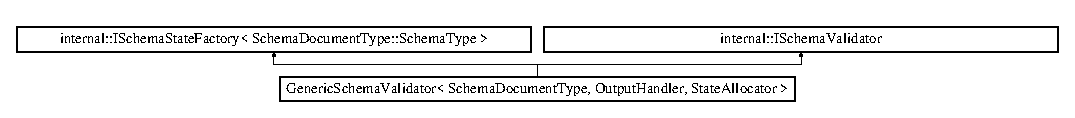
\includegraphics[height=1.135903cm]{a02244}
\end{center}
\end{figure}
\subsection*{Public Types}
\begin{DoxyCompactItemize}
\item 
\mbox{\Hypertarget{a02244_ac79628f00f6720bbabb70b44f0d076a0}\label{a02244_ac79628f00f6720bbabb70b44f0d076a0}} 
typedef Schema\+Document\+Type\+::\+Schema\+Type {\bfseries Schema\+Type}
\item 
\mbox{\Hypertarget{a02244_ae0c6c9a9c0ff6bae80e75c6705f2668b}\label{a02244_ae0c6c9a9c0ff6bae80e75c6705f2668b}} 
typedef Schema\+Document\+Type\+::\+Pointer\+Type {\bfseries Pointer\+Type}
\item 
\mbox{\Hypertarget{a02244_acf1c5361bb96da87d23167d8720b1ea5}\label{a02244_acf1c5361bb96da87d23167d8720b1ea5}} 
typedef Schema\+Type\+::\+Encoding\+Type {\bfseries Encoding\+Type}
\item 
\mbox{\Hypertarget{a02244_a8b7dab5a0cda9cc0adaefb4401d260c1}\label{a02244_a8b7dab5a0cda9cc0adaefb4401d260c1}} 
typedef Encoding\+Type\+::\+Ch {\bfseries Ch}
\end{DoxyCompactItemize}
\subsection*{Public Member Functions}
\begin{DoxyCompactItemize}
\item 
\hyperlink{a02244_a202ee6fdbe5ae9eab3e77a81ecdfeb6d}{Generic\+Schema\+Validator} (const Schema\+Document\+Type \&schema\+Document, State\+Allocator $\ast$allocator=0, size\+\_\+t schema\+Stack\+Capacity=k\+Default\+Schema\+Stack\+Capacity, size\+\_\+t document\+Stack\+Capacity=k\+Default\+Document\+Stack\+Capacity)
\begin{DoxyCompactList}\small\item\em Constructor without output handler. \end{DoxyCompactList}\item 
\hyperlink{a02244_ac2027be8ca55b01cd6f38b45f4e233b4}{Generic\+Schema\+Validator} (const Schema\+Document\+Type \&schema\+Document, Output\+Handler \&output\+Handler, State\+Allocator $\ast$allocator=0, size\+\_\+t schema\+Stack\+Capacity=k\+Default\+Schema\+Stack\+Capacity, size\+\_\+t document\+Stack\+Capacity=k\+Default\+Document\+Stack\+Capacity)
\begin{DoxyCompactList}\small\item\em Constructor with output handler. \end{DoxyCompactList}\item 
\mbox{\Hypertarget{a02244_a3eab83d483a50efb0c0390adf3291963}\label{a02244_a3eab83d483a50efb0c0390adf3291963}} 
\hyperlink{a02244_a3eab83d483a50efb0c0390adf3291963}{$\sim$\+Generic\+Schema\+Validator} ()
\begin{DoxyCompactList}\small\item\em Destructor. \end{DoxyCompactList}\item 
\mbox{\Hypertarget{a02244_a49efbbe098cb77728be3d48cafed17e4}\label{a02244_a49efbbe098cb77728be3d48cafed17e4}} 
void \hyperlink{a02244_a49efbbe098cb77728be3d48cafed17e4}{Reset} ()
\begin{DoxyCompactList}\small\item\em Reset the internal states. \end{DoxyCompactList}\item 
\mbox{\Hypertarget{a02244_a8ebda4da3d8b1fc41e57f15dd62e8f19}\label{a02244_a8ebda4da3d8b1fc41e57f15dd62e8f19}} 
virtual bool \hyperlink{a02244_a8ebda4da3d8b1fc41e57f15dd62e8f19}{Is\+Valid} () const
\begin{DoxyCompactList}\small\item\em Checks whether the current state is valid. \end{DoxyCompactList}\item 
\mbox{\Hypertarget{a02244_a5b8f2d5c466b2a362e2e4c3bcfbfc5a8}\label{a02244_a5b8f2d5c466b2a362e2e4c3bcfbfc5a8}} 
Pointer\+Type \hyperlink{a02244_a5b8f2d5c466b2a362e2e4c3bcfbfc5a8}{Get\+Invalid\+Schema\+Pointer} () const
\begin{DoxyCompactList}\small\item\em Gets the J\+S\+ON pointer pointed to the invalid schema. \end{DoxyCompactList}\item 
\mbox{\Hypertarget{a02244_ab71ec18e5a013e5153a10b312a4f03bc}\label{a02244_ab71ec18e5a013e5153a10b312a4f03bc}} 
const Ch $\ast$ \hyperlink{a02244_ab71ec18e5a013e5153a10b312a4f03bc}{Get\+Invalid\+Schema\+Keyword} () const
\begin{DoxyCompactList}\small\item\em Gets the keyword of invalid schema. \end{DoxyCompactList}\item 
\mbox{\Hypertarget{a02244_ac10a88c4dc138bbdbe2afd041658a3b0}\label{a02244_ac10a88c4dc138bbdbe2afd041658a3b0}} 
Pointer\+Type \hyperlink{a02244_ac10a88c4dc138bbdbe2afd041658a3b0}{Get\+Invalid\+Document\+Pointer} () const
\begin{DoxyCompactList}\small\item\em Gets the J\+S\+ON pointer pointed to the invalid value. \end{DoxyCompactList}\item 
\mbox{\Hypertarget{a02244_a7137af73e934f50c66cbb8a9aa802ea6}\label{a02244_a7137af73e934f50c66cbb8a9aa802ea6}} 
bool {\bfseries Null} ()
\item 
\mbox{\Hypertarget{a02244_aa25fa7456f2f308a105e400f01a4afde}\label{a02244_aa25fa7456f2f308a105e400f01a4afde}} 
bool {\bfseries Bool} (bool b)
\item 
\mbox{\Hypertarget{a02244_ad823c29990225661a4df69d34647b659}\label{a02244_ad823c29990225661a4df69d34647b659}} 
bool {\bfseries Int} (int i)
\item 
\mbox{\Hypertarget{a02244_aa688665c5274f93543c84a4b6cabe8da}\label{a02244_aa688665c5274f93543c84a4b6cabe8da}} 
bool {\bfseries Uint} (unsigned u)
\item 
\mbox{\Hypertarget{a02244_ac5a9e416e18129a7b787f251019a828f}\label{a02244_ac5a9e416e18129a7b787f251019a828f}} 
bool {\bfseries Int64} (int64\+\_\+t i)
\item 
\mbox{\Hypertarget{a02244_abfc56c58cf0b65318e376fc5f2879292}\label{a02244_abfc56c58cf0b65318e376fc5f2879292}} 
bool {\bfseries Uint64} (uint64\+\_\+t u)
\item 
\mbox{\Hypertarget{a02244_aed0532dbda3ac6f3ca7196af06066b86}\label{a02244_aed0532dbda3ac6f3ca7196af06066b86}} 
bool {\bfseries Double} (double d)
\item 
\mbox{\Hypertarget{a02244_ae4f024145421d2c1dde08a9de528722a}\label{a02244_ae4f024145421d2c1dde08a9de528722a}} 
bool {\bfseries Raw\+Number} (const Ch $\ast$str, \hyperlink{a00560_a5ed6e6e67250fadbd041127e6386dcb5}{Size\+Type} length, bool copy)
\item 
\mbox{\Hypertarget{a02244_a33cf3f83307a8fea38c3238ef75c3d58}\label{a02244_a33cf3f83307a8fea38c3238ef75c3d58}} 
bool {\bfseries String} (const Ch $\ast$str, \hyperlink{a00560_a5ed6e6e67250fadbd041127e6386dcb5}{Size\+Type} length, bool copy)
\item 
\mbox{\Hypertarget{a02244_a59972d612c3d37aae9a30222e428d216}\label{a02244_a59972d612c3d37aae9a30222e428d216}} 
bool {\bfseries Start\+Object} ()
\item 
\mbox{\Hypertarget{a02244_a6d08b458216ec4a09eed9d94800d05c1}\label{a02244_a6d08b458216ec4a09eed9d94800d05c1}} 
bool {\bfseries Key} (const Ch $\ast$str, \hyperlink{a00560_a5ed6e6e67250fadbd041127e6386dcb5}{Size\+Type} len, bool copy)
\item 
\mbox{\Hypertarget{a02244_aa89e14f0f731f6acdec22a0f7e003037}\label{a02244_aa89e14f0f731f6acdec22a0f7e003037}} 
bool {\bfseries End\+Object} (\hyperlink{a00560_a5ed6e6e67250fadbd041127e6386dcb5}{Size\+Type} member\+Count)
\item 
\mbox{\Hypertarget{a02244_aba13751f802531ed8cbd850778ea993c}\label{a02244_aba13751f802531ed8cbd850778ea993c}} 
bool {\bfseries Start\+Array} ()
\item 
\mbox{\Hypertarget{a02244_a67b501f0f65d40e0086ca8216882b34f}\label{a02244_a67b501f0f65d40e0086ca8216882b34f}} 
bool {\bfseries End\+Array} (\hyperlink{a00560_a5ed6e6e67250fadbd041127e6386dcb5}{Size\+Type} element\+Count)
\item 
\mbox{\Hypertarget{a02244_af074f9c8f2cfc07e1b3d3f8862e7ef11}\label{a02244_af074f9c8f2cfc07e1b3d3f8862e7ef11}} 
virtual I\+Schema\+Validator $\ast$ {\bfseries Create\+Schema\+Validator} (const Schema\+Type \&root)
\item 
\mbox{\Hypertarget{a02244_ae24fa298e328f1fd7dda2ef6267156d2}\label{a02244_ae24fa298e328f1fd7dda2ef6267156d2}} 
virtual void {\bfseries Destroy\+Schema\+Validator} (I\+Schema\+Validator $\ast$validator)
\item 
\mbox{\Hypertarget{a02244_abc377481583ca2095fb784be88887faa}\label{a02244_abc377481583ca2095fb784be88887faa}} 
virtual void $\ast$ {\bfseries Create\+Hasher} ()
\item 
\mbox{\Hypertarget{a02244_ac01c45982a1f512e1ca06fe5544b0c0f}\label{a02244_ac01c45982a1f512e1ca06fe5544b0c0f}} 
virtual uint64\+\_\+t {\bfseries Get\+Hash\+Code} (void $\ast$hasher)
\item 
\mbox{\Hypertarget{a02244_a007eef58be575dc562543d069ddd2710}\label{a02244_a007eef58be575dc562543d069ddd2710}} 
virtual void {\bfseries Destrory\+Hasher} (void $\ast$hasher)
\item 
\mbox{\Hypertarget{a02244_a7c999dfb3118aaa08495d60eee6d3732}\label{a02244_a7c999dfb3118aaa08495d60eee6d3732}} 
virtual void $\ast$ {\bfseries Malloc\+State} (size\+\_\+t size)
\item 
\mbox{\Hypertarget{a02244_a4e250737a411af2969a9e585a7da4187}\label{a02244_a4e250737a411af2969a9e585a7da4187}} 
virtual void {\bfseries Free\+State} (void $\ast$p)
\end{DoxyCompactItemize}


\subsection{Detailed Description}
\subsubsection*{template$<$typename Schema\+Document\+Type, typename Output\+Handler = Base\+Reader\+Handler$<$typename Schema\+Document\+Type\+::\+Schema\+Type\+::\+Encoding\+Type$>$, typename State\+Allocator = Crt\+Allocator$>$\newline
class Generic\+Schema\+Validator$<$ Schema\+Document\+Type, Output\+Handler, State\+Allocator $>$}

J\+S\+ON Schema Validator. 

A S\+AX style J\+S\+ON schema validator. It uses a {\ttfamily \hyperlink{a02240}{Generic\+Schema\+Document}} to validate S\+AX events. It delegates the incoming S\+AX events to an output handler. The default output handler does nothing. It can be reused multiple times by calling {\ttfamily \hyperlink{a02244_a49efbbe098cb77728be3d48cafed17e4}{Reset()}}.


\begin{DoxyTemplParams}{Template Parameters}
{\em Schema\+Document\+Type} & Type of schema document. \\
\hline
{\em Output\+Handler} & Type of output handler. Default handler does nothing. \\
\hline
{\em State\+Allocator} & Allocator for storing the internal validation states. \\
\hline
\end{DoxyTemplParams}


\subsection{Constructor \& Destructor Documentation}
\mbox{\Hypertarget{a02244_a202ee6fdbe5ae9eab3e77a81ecdfeb6d}\label{a02244_a202ee6fdbe5ae9eab3e77a81ecdfeb6d}} 
\index{Generic\+Schema\+Validator@{Generic\+Schema\+Validator}!Generic\+Schema\+Validator@{Generic\+Schema\+Validator}}
\index{Generic\+Schema\+Validator@{Generic\+Schema\+Validator}!Generic\+Schema\+Validator@{Generic\+Schema\+Validator}}
\subsubsection{\texorpdfstring{Generic\+Schema\+Validator()}{GenericSchemaValidator()}\hspace{0.1cm}{\footnotesize\ttfamily [1/2]}}
{\footnotesize\ttfamily template$<$typename Schema\+Document\+Type, typename Output\+Handler = Base\+Reader\+Handler$<$typename Schema\+Document\+Type\+::\+Schema\+Type\+::\+Encoding\+Type$>$, typename State\+Allocator = Crt\+Allocator$>$ \\
\hyperlink{a02244}{Generic\+Schema\+Validator}$<$ Schema\+Document\+Type, Output\+Handler, State\+Allocator $>$\+::\hyperlink{a02244}{Generic\+Schema\+Validator} (\begin{DoxyParamCaption}\item[{const Schema\+Document\+Type \&}]{schema\+Document,  }\item[{State\+Allocator $\ast$}]{allocator = {\ttfamily 0},  }\item[{size\+\_\+t}]{schema\+Stack\+Capacity = {\ttfamily kDefaultSchemaStackCapacity},  }\item[{size\+\_\+t}]{document\+Stack\+Capacity = {\ttfamily kDefaultDocumentStackCapacity} }\end{DoxyParamCaption})\hspace{0.3cm}{\ttfamily [inline]}}



Constructor without output handler. 


\begin{DoxyParams}{Parameters}
{\em schema\+Document} & The schema document to conform to. \\
\hline
{\em allocator} & Optional allocator for storing internal validation states. \\
\hline
{\em schema\+Stack\+Capacity} & Optional initial capacity of schema path stack. \\
\hline
{\em document\+Stack\+Capacity} & Optional initial capacity of document path stack. \\
\hline
\end{DoxyParams}
\mbox{\Hypertarget{a02244_ac2027be8ca55b01cd6f38b45f4e233b4}\label{a02244_ac2027be8ca55b01cd6f38b45f4e233b4}} 
\index{Generic\+Schema\+Validator@{Generic\+Schema\+Validator}!Generic\+Schema\+Validator@{Generic\+Schema\+Validator}}
\index{Generic\+Schema\+Validator@{Generic\+Schema\+Validator}!Generic\+Schema\+Validator@{Generic\+Schema\+Validator}}
\subsubsection{\texorpdfstring{Generic\+Schema\+Validator()}{GenericSchemaValidator()}\hspace{0.1cm}{\footnotesize\ttfamily [2/2]}}
{\footnotesize\ttfamily template$<$typename Schema\+Document\+Type, typename Output\+Handler = Base\+Reader\+Handler$<$typename Schema\+Document\+Type\+::\+Schema\+Type\+::\+Encoding\+Type$>$, typename State\+Allocator = Crt\+Allocator$>$ \\
\hyperlink{a02244}{Generic\+Schema\+Validator}$<$ Schema\+Document\+Type, Output\+Handler, State\+Allocator $>$\+::\hyperlink{a02244}{Generic\+Schema\+Validator} (\begin{DoxyParamCaption}\item[{const Schema\+Document\+Type \&}]{schema\+Document,  }\item[{Output\+Handler \&}]{output\+Handler,  }\item[{State\+Allocator $\ast$}]{allocator = {\ttfamily 0},  }\item[{size\+\_\+t}]{schema\+Stack\+Capacity = {\ttfamily kDefaultSchemaStackCapacity},  }\item[{size\+\_\+t}]{document\+Stack\+Capacity = {\ttfamily kDefaultDocumentStackCapacity} }\end{DoxyParamCaption})\hspace{0.3cm}{\ttfamily [inline]}}



Constructor with output handler. 


\begin{DoxyParams}{Parameters}
{\em schema\+Document} & The schema document to conform to. \\
\hline
{\em allocator} & Optional allocator for storing internal validation states. \\
\hline
{\em schema\+Stack\+Capacity} & Optional initial capacity of schema path stack. \\
\hline
{\em document\+Stack\+Capacity} & Optional initial capacity of document path stack. \\
\hline
\end{DoxyParams}


The documentation for this class was generated from the following files\+:\begin{DoxyCompactItemize}
\item 
fwd.\+h\item 
schema.\+h\end{DoxyCompactItemize}

\hypertarget{a02208}{}\section{Generic\+String\+Buffer$<$ Encoding, Allocator $>$ Class Template Reference}
\label{a02208}\index{Generic\+String\+Buffer$<$ Encoding, Allocator $>$@{Generic\+String\+Buffer$<$ Encoding, Allocator $>$}}


Represents an in-\/memory output stream.  




{\ttfamily \#include $<$stringbuffer.\+h$>$}

\subsection*{Public Types}
\begin{DoxyCompactItemize}
\item 
\mbox{\Hypertarget{a02208_a735b75db076ffe86d0d294be49655d46}\label{a02208_a735b75db076ffe86d0d294be49655d46}} 
typedef Encoding\+::\+Ch {\bfseries Ch}
\end{DoxyCompactItemize}
\subsection*{Public Member Functions}
\begin{DoxyCompactItemize}
\item 
\mbox{\Hypertarget{a02208_a62f5ea1a53a2a3f98088f8c152b6183e}\label{a02208_a62f5ea1a53a2a3f98088f8c152b6183e}} 
{\bfseries Generic\+String\+Buffer} (Allocator $\ast$allocator=0, size\+\_\+t capacity=k\+Default\+Capacity)
\item 
\mbox{\Hypertarget{a02208_a8be5c8fadccacdcf40e20220f38e0afa}\label{a02208_a8be5c8fadccacdcf40e20220f38e0afa}} 
void {\bfseries Put} (Ch c)
\item 
\mbox{\Hypertarget{a02208_a9225468d11fdddfc3a9a4e48bf4d3ba4}\label{a02208_a9225468d11fdddfc3a9a4e48bf4d3ba4}} 
void {\bfseries Put\+Unsafe} (Ch c)
\item 
\mbox{\Hypertarget{a02208_a28bb539487db17b07314a532f3b8847c}\label{a02208_a28bb539487db17b07314a532f3b8847c}} 
void {\bfseries Flush} ()
\item 
\mbox{\Hypertarget{a02208_a42f15c959046d899cb74c3120a6995f9}\label{a02208_a42f15c959046d899cb74c3120a6995f9}} 
void {\bfseries Clear} ()
\item 
\mbox{\Hypertarget{a02208_a0dbdb77489b95923795011a24f705be5}\label{a02208_a0dbdb77489b95923795011a24f705be5}} 
void {\bfseries Shrink\+To\+Fit} ()
\item 
\mbox{\Hypertarget{a02208_a4d6becae201b98c122746298882a318f}\label{a02208_a4d6becae201b98c122746298882a318f}} 
void {\bfseries Reserve} (size\+\_\+t count)
\item 
\mbox{\Hypertarget{a02208_a49fd10cdd5dd97a4cf9813d01334d660}\label{a02208_a49fd10cdd5dd97a4cf9813d01334d660}} 
Ch $\ast$ {\bfseries Push} (size\+\_\+t count)
\item 
\mbox{\Hypertarget{a02208_a4e396f55323ca54f949685c7c6ef2060}\label{a02208_a4e396f55323ca54f949685c7c6ef2060}} 
Ch $\ast$ {\bfseries Push\+Unsafe} (size\+\_\+t count)
\item 
\mbox{\Hypertarget{a02208_a0038e53ba03c271bc4cbbac403ec4de4}\label{a02208_a0038e53ba03c271bc4cbbac403ec4de4}} 
void {\bfseries Pop} (size\+\_\+t count)
\item 
\mbox{\Hypertarget{a02208_ab06b8c5f1385bd3dfd4caea8b7510f0b}\label{a02208_ab06b8c5f1385bd3dfd4caea8b7510f0b}} 
const Ch $\ast$ {\bfseries Get\+String} () const
\item 
\mbox{\Hypertarget{a02208_a725e862b9a78375f5363b0b61ad789f3}\label{a02208_a725e862b9a78375f5363b0b61ad789f3}} 
size\+\_\+t \hyperlink{a02208_a725e862b9a78375f5363b0b61ad789f3}{Get\+Size} () const
\begin{DoxyCompactList}\small\item\em Get the size of string in bytes in the string buffer. \end{DoxyCompactList}\item 
\mbox{\Hypertarget{a02208_ad324b8154be3354dda3aa4a0a7361499}\label{a02208_ad324b8154be3354dda3aa4a0a7361499}} 
size\+\_\+t \hyperlink{a02208_ad324b8154be3354dda3aa4a0a7361499}{Get\+Length} () const
\begin{DoxyCompactList}\small\item\em Get the length of string in Ch in the string buffer. \end{DoxyCompactList}\end{DoxyCompactItemize}
\subsection*{Public Attributes}
\begin{DoxyCompactItemize}
\item 
\mbox{\Hypertarget{a02208_aaef716643febb9de5957dbf8ff904409}\label{a02208_aaef716643febb9de5957dbf8ff904409}} 
\hyperlink{a02288}{internal\+::\+Stack}$<$ Allocator $>$ {\bfseries stack\+\_\+}
\end{DoxyCompactItemize}
\subsection*{Static Public Attributes}
\begin{DoxyCompactItemize}
\item 
\mbox{\Hypertarget{a02208_ae74f9df854dd5a7db4315ef44b016d22}\label{a02208_ae74f9df854dd5a7db4315ef44b016d22}} 
static const size\+\_\+t {\bfseries k\+Default\+Capacity} = 256
\end{DoxyCompactItemize}


\subsection{Detailed Description}
\subsubsection*{template$<$typename Encoding, typename Allocator = Crt\+Allocator$>$\newline
class Generic\+String\+Buffer$<$ Encoding, Allocator $>$}

Represents an in-\/memory output stream. 


\begin{DoxyTemplParams}{Template Parameters}
{\em Encoding} & Encoding of the stream. \\
\hline
{\em Allocator} & type for allocating memory buffer. \\
\hline
\end{DoxyTemplParams}
\begin{DoxyNote}{Note}
implements Stream concept 
\end{DoxyNote}


The documentation for this class was generated from the following files\+:\begin{DoxyCompactItemize}
\item 
fwd.\+h\item 
stringbuffer.\+h\end{DoxyCompactItemize}

\hypertarget{a02008}{}\section{Generic\+String\+Ref$<$ Char\+Type $>$ Struct Template Reference}
\label{a02008}\index{Generic\+String\+Ref$<$ Char\+Type $>$@{Generic\+String\+Ref$<$ Char\+Type $>$}}


Reference to a constant string (not taking a copy)  




{\ttfamily \#include $<$document.\+h$>$}

\subsection*{Public Types}
\begin{DoxyCompactItemize}
\item 
\mbox{\Hypertarget{a02008_a16908c3fce41be380061330c14ba2140}\label{a02008_a16908c3fce41be380061330c14ba2140}} 
typedef Char\+Type \hyperlink{a02008_a16908c3fce41be380061330c14ba2140}{Ch}
\begin{DoxyCompactList}\small\item\em character type of the string \end{DoxyCompactList}\end{DoxyCompactItemize}
\subsection*{Public Member Functions}
\begin{DoxyCompactItemize}
\item 
{\footnotesize template$<$Size\+Type N$>$ }\\\hyperlink{a02008_aae0c070f914d2486a560150a927c22dc}{Generic\+String\+Ref} (const Char\+Type(\&str)\mbox{[}N\mbox{]}) R\+A\+P\+I\+D\+J\+S\+O\+N\+\_\+\+N\+O\+E\+X\+C\+E\+PT
\begin{DoxyCompactList}\small\item\em Create string reference from {\ttfamily const} character array. \end{DoxyCompactList}\item 
\hyperlink{a02008_a9e80d81d5ad49cf0fb4128ace8c548d9}{Generic\+String\+Ref} (const Char\+Type $\ast$str)
\begin{DoxyCompactList}\small\item\em Explicitly create string reference from {\ttfamily const} character pointer. \end{DoxyCompactList}\item 
\hyperlink{a02008_a8b2c6a7fdc4da1e7055f7fdcf0ac517f}{Generic\+String\+Ref} (const Char\+Type $\ast$str, \hyperlink{a00560_a5ed6e6e67250fadbd041127e6386dcb5}{Size\+Type} len)
\begin{DoxyCompactList}\small\item\em Create constant string reference from pointer and length. \end{DoxyCompactList}\item 
\mbox{\Hypertarget{a02008_ab049693082c0b8f5066c00212e780aec}\label{a02008_ab049693082c0b8f5066c00212e780aec}} 
{\bfseries Generic\+String\+Ref} (const \hyperlink{a02008}{Generic\+String\+Ref} \&rhs)
\item 
\mbox{\Hypertarget{a02008_a4e652ee3a398d0eb8ece1835d15274d0}\label{a02008_a4e652ee3a398d0eb8ece1835d15274d0}} 
\hyperlink{a02008_a4e652ee3a398d0eb8ece1835d15274d0}{operator const Ch $\ast$} () const
\begin{DoxyCompactList}\small\item\em implicit conversion to plain Char\+Type pointer \end{DoxyCompactList}\end{DoxyCompactItemize}
\subsection*{Public Attributes}
\begin{DoxyCompactItemize}
\item 
\mbox{\Hypertarget{a02008_ac555994afd329bc9bc1780acf2f9d9be}\label{a02008_ac555994afd329bc9bc1780acf2f9d9be}} 
const \hyperlink{a02008_a16908c3fce41be380061330c14ba2140}{Ch} $\ast$const \hyperlink{a02008_ac555994afd329bc9bc1780acf2f9d9be}{s}
\begin{DoxyCompactList}\small\item\em plain Char\+Type pointer \end{DoxyCompactList}\item 
\mbox{\Hypertarget{a02008_a4a96d618744ad73f766a1551b1d517fe}\label{a02008_a4a96d618744ad73f766a1551b1d517fe}} 
const \hyperlink{a00560_a5ed6e6e67250fadbd041127e6386dcb5}{Size\+Type} \hyperlink{a02008_a4a96d618744ad73f766a1551b1d517fe}{length}
\begin{DoxyCompactList}\small\item\em length of the string (excluding the trailing N\+U\+LL terminator) \end{DoxyCompactList}\end{DoxyCompactItemize}
\subsection*{Related Functions}
(Note that these are not member functions.) \begin{DoxyCompactItemize}
\item 
{\footnotesize template$<$typename Char\+Type $>$ }\\\hyperlink{a02008}{Generic\+String\+Ref}$<$ Char\+Type $>$ \hyperlink{a02008_aa6b9fd9f6aa49405a574c362ba9af6b5}{String\+Ref} (const Char\+Type $\ast$str)
\begin{DoxyCompactList}\small\item\em Mark a character pointer as constant string. \end{DoxyCompactList}\item 
{\footnotesize template$<$typename Char\+Type $>$ }\\\hyperlink{a02008}{Generic\+String\+Ref}$<$ Char\+Type $>$ \hyperlink{a02008_a578c51ab574a50a9c760b9da7c7562f2}{String\+Ref} (const Char\+Type $\ast$str, size\+\_\+t \hyperlink{a02008_a4a96d618744ad73f766a1551b1d517fe}{length})
\begin{DoxyCompactList}\small\item\em Mark a character pointer as constant string. \end{DoxyCompactList}\end{DoxyCompactItemize}


\subsection{Detailed Description}
\subsubsection*{template$<$typename Char\+Type$>$\newline
struct Generic\+String\+Ref$<$ Char\+Type $>$}

Reference to a constant string (not taking a copy) 


\begin{DoxyTemplParams}{Template Parameters}
{\em Char\+Type} & character type of the string\\
\hline
\end{DoxyTemplParams}
This helper class is used to automatically infer constant string references for string literals, especially from {\ttfamily const} {\bfseries }(!) character arrays.

The main use is for creating J\+S\+ON string values without copying the source string via an Allocator. This requires that the referenced string pointers have a sufficient lifetime, which exceeds the lifetime of the associated \hyperlink{a01992}{Generic\+Value}.

{\bfseries Example} 
\begin{DoxyCode}
\hyperlink{a01992}{Value} v(\textcolor{stringliteral}{"foo"});   \textcolor{comment}{// ok, no need to copy & calculate length}
\textcolor{keyword}{const} \textcolor{keywordtype}{char} foo[] = \textcolor{stringliteral}{"foo"};
v.SetString(foo); \textcolor{comment}{// ok}

\textcolor{keyword}{const} \textcolor{keywordtype}{char}* bar = foo;
\textcolor{comment}{// Value x(bar); // not ok, can't rely on bar's lifetime}
\hyperlink{a01992}{Value} x(\hyperlink{a02008_aa6b9fd9f6aa49405a574c362ba9af6b5}{StringRef}(bar)); \textcolor{comment}{// lifetime explicitly guaranteed by user}
\hyperlink{a01992}{Value} y(\hyperlink{a02008_aa6b9fd9f6aa49405a574c362ba9af6b5}{StringRef}(bar, 3));  \textcolor{comment}{// ok, explicitly pass length}
\end{DoxyCode}


\begin{DoxySeeAlso}{See also}
\hyperlink{a02008_aa6b9fd9f6aa49405a574c362ba9af6b5}{String\+Ref}, Generic\+Value\+::\+Set\+String 
\end{DoxySeeAlso}


\subsection{Constructor \& Destructor Documentation}
\mbox{\Hypertarget{a02008_aae0c070f914d2486a560150a927c22dc}\label{a02008_aae0c070f914d2486a560150a927c22dc}} 
\index{Generic\+String\+Ref@{Generic\+String\+Ref}!Generic\+String\+Ref@{Generic\+String\+Ref}}
\index{Generic\+String\+Ref@{Generic\+String\+Ref}!Generic\+String\+Ref@{Generic\+String\+Ref}}
\subsubsection{\texorpdfstring{Generic\+String\+Ref()}{GenericStringRef()}\hspace{0.1cm}{\footnotesize\ttfamily [1/3]}}
{\footnotesize\ttfamily template$<$typename Char\+Type$>$ \\
template$<$Size\+Type N$>$ \\
\hyperlink{a02008}{Generic\+String\+Ref}$<$ Char\+Type $>$\+::\hyperlink{a02008}{Generic\+String\+Ref} (\begin{DoxyParamCaption}\item[{const Char\+Type(\&)}]{str\mbox{[}\+N\mbox{]} }\end{DoxyParamCaption})\hspace{0.3cm}{\ttfamily [inline]}}



Create string reference from {\ttfamily const} character array. 

This constructor implicitly creates a constant string reference from a {\ttfamily const} character array. It has better performance than \hyperlink{a02008_aa6b9fd9f6aa49405a574c362ba9af6b5}{String\+Ref(const Char\+Type$\ast$)} by inferring the string \hyperlink{a02008_a4a96d618744ad73f766a1551b1d517fe}{length} from the array length, and also supports strings containing null characters.


\begin{DoxyTemplParams}{Template Parameters}
{\em N} & length of the string, automatically inferred\\
\hline
\end{DoxyTemplParams}

\begin{DoxyParams}{Parameters}
{\em str} & Constant character array, lifetime assumed to be longer than the use of the string in e.\+g. a \hyperlink{a01992}{Generic\+Value}\\
\hline
\end{DoxyParams}
\begin{DoxyPostcond}{Postcondition}
\hyperlink{a02008_ac555994afd329bc9bc1780acf2f9d9be}{s} == str
\end{DoxyPostcond}
\begin{DoxyNote}{Note}
Constant complexity. 

There is a hidden, private overload to disallow references to non-\/const character arrays to be created via this constructor. By this, e.\+g. function-\/scope arrays used to be filled via {\ttfamily snprintf} are excluded from consideration. In such cases, the referenced string should be {\bfseries copied} to the \hyperlink{a01992}{Generic\+Value} instead. 
\end{DoxyNote}
\mbox{\Hypertarget{a02008_a9e80d81d5ad49cf0fb4128ace8c548d9}\label{a02008_a9e80d81d5ad49cf0fb4128ace8c548d9}} 
\index{Generic\+String\+Ref@{Generic\+String\+Ref}!Generic\+String\+Ref@{Generic\+String\+Ref}}
\index{Generic\+String\+Ref@{Generic\+String\+Ref}!Generic\+String\+Ref@{Generic\+String\+Ref}}
\subsubsection{\texorpdfstring{Generic\+String\+Ref()}{GenericStringRef()}\hspace{0.1cm}{\footnotesize\ttfamily [2/3]}}
{\footnotesize\ttfamily template$<$typename Char\+Type$>$ \\
\hyperlink{a02008}{Generic\+String\+Ref}$<$ Char\+Type $>$\+::\hyperlink{a02008}{Generic\+String\+Ref} (\begin{DoxyParamCaption}\item[{const Char\+Type $\ast$}]{str }\end{DoxyParamCaption})\hspace{0.3cm}{\ttfamily [inline]}, {\ttfamily [explicit]}}



Explicitly create string reference from {\ttfamily const} character pointer. 

This constructor can be used to {\bfseries explicitly} create a reference to a constant string pointer.

\begin{DoxySeeAlso}{See also}
\hyperlink{a02008_aa6b9fd9f6aa49405a574c362ba9af6b5}{String\+Ref(const Char\+Type$\ast$)}
\end{DoxySeeAlso}

\begin{DoxyParams}{Parameters}
{\em str} & Constant character pointer, lifetime assumed to be longer than the use of the string in e.\+g. a \hyperlink{a01992}{Generic\+Value}\\
\hline
\end{DoxyParams}
\begin{DoxyPostcond}{Postcondition}
\hyperlink{a02008_ac555994afd329bc9bc1780acf2f9d9be}{s} == str
\end{DoxyPostcond}
\begin{DoxyNote}{Note}
There is a hidden, private overload to disallow references to non-\/const character arrays to be created via this constructor. By this, e.\+g. function-\/scope arrays used to be filled via {\ttfamily snprintf} are excluded from consideration. In such cases, the referenced string should be {\bfseries copied} to the \hyperlink{a01992}{Generic\+Value} instead. 
\end{DoxyNote}
\mbox{\Hypertarget{a02008_a8b2c6a7fdc4da1e7055f7fdcf0ac517f}\label{a02008_a8b2c6a7fdc4da1e7055f7fdcf0ac517f}} 
\index{Generic\+String\+Ref@{Generic\+String\+Ref}!Generic\+String\+Ref@{Generic\+String\+Ref}}
\index{Generic\+String\+Ref@{Generic\+String\+Ref}!Generic\+String\+Ref@{Generic\+String\+Ref}}
\subsubsection{\texorpdfstring{Generic\+String\+Ref()}{GenericStringRef()}\hspace{0.1cm}{\footnotesize\ttfamily [3/3]}}
{\footnotesize\ttfamily template$<$typename Char\+Type$>$ \\
\hyperlink{a02008}{Generic\+String\+Ref}$<$ Char\+Type $>$\+::\hyperlink{a02008}{Generic\+String\+Ref} (\begin{DoxyParamCaption}\item[{const Char\+Type $\ast$}]{str,  }\item[{\hyperlink{a00560_a5ed6e6e67250fadbd041127e6386dcb5}{Size\+Type}}]{len }\end{DoxyParamCaption})\hspace{0.3cm}{\ttfamily [inline]}}



Create constant string reference from pointer and length. 


\begin{DoxyParams}{Parameters}
{\em str} & constant string, lifetime assumed to be longer than the use of the string in e.\+g. a \hyperlink{a01992}{Generic\+Value} \\
\hline
{\em len} & length of the string, excluding the trailing N\+U\+LL terminator\\
\hline
\end{DoxyParams}
\begin{DoxyPostcond}{Postcondition}
\hyperlink{a02008_ac555994afd329bc9bc1780acf2f9d9be}{s} == str \&\& \hyperlink{a02008_a4a96d618744ad73f766a1551b1d517fe}{length} == len 
\end{DoxyPostcond}
\begin{DoxyNote}{Note}
Constant complexity. 
\end{DoxyNote}


\subsection{Friends And Related Function Documentation}
\mbox{\Hypertarget{a02008_aa6b9fd9f6aa49405a574c362ba9af6b5}\label{a02008_aa6b9fd9f6aa49405a574c362ba9af6b5}} 
\index{Generic\+String\+Ref@{Generic\+String\+Ref}!String\+Ref@{String\+Ref}}
\index{String\+Ref@{String\+Ref}!Generic\+String\+Ref@{Generic\+String\+Ref}}
\subsubsection{\texorpdfstring{String\+Ref()}{StringRef()}\hspace{0.1cm}{\footnotesize\ttfamily [1/2]}}
{\footnotesize\ttfamily template$<$typename Char\+Type $>$ \\
\hyperlink{a02008}{Generic\+String\+Ref}$<$ Char\+Type $>$ String\+Ref (\begin{DoxyParamCaption}\item[{const Char\+Type $\ast$}]{str }\end{DoxyParamCaption})\hspace{0.3cm}{\ttfamily [related]}}



Mark a character pointer as constant string. 

Mark a plain character pointer as a \char`\"{}string literal\char`\"{}. This function can be used to avoid copying a character string to be referenced as a value in a J\+S\+ON \hyperlink{a01992}{Generic\+Value} object, if the string\textquotesingle{}s lifetime is known to be valid long enough. 
\begin{DoxyTemplParams}{Template Parameters}
{\em Char\+Type} & Character type of the string \\
\hline
\end{DoxyTemplParams}

\begin{DoxyParams}{Parameters}
{\em str} & Constant string, lifetime assumed to be longer than the use of the string in e.\+g. a \hyperlink{a01992}{Generic\+Value} \\
\hline
\end{DoxyParams}
\begin{DoxyReturn}{Returns}
\hyperlink{a02008}{Generic\+String\+Ref} string reference object
\end{DoxyReturn}
\begin{DoxySeeAlso}{See also}
\hyperlink{a01992_abb2887958974fef1b2b5c8e32cc72ddb}{Generic\+Value\+::\+Generic\+Value(\+String\+Ref\+Type)}, \hyperlink{a01992_a386708557555e6389184de608af5e6a6}{Generic\+Value\+::operator=(\+String\+Ref\+Type)}, Generic\+Value\+::\+Set\+String(\+String\+Ref\+Type), Generic\+Value\+::\+Push\+Back(\+String\+Ref\+Type, Allocator\&), Generic\+Value\+::\+Add\+Member 
\end{DoxySeeAlso}
\mbox{\Hypertarget{a02008_a578c51ab574a50a9c760b9da7c7562f2}\label{a02008_a578c51ab574a50a9c760b9da7c7562f2}} 
\index{Generic\+String\+Ref@{Generic\+String\+Ref}!String\+Ref@{String\+Ref}}
\index{String\+Ref@{String\+Ref}!Generic\+String\+Ref@{Generic\+String\+Ref}}
\subsubsection{\texorpdfstring{String\+Ref()}{StringRef()}\hspace{0.1cm}{\footnotesize\ttfamily [2/2]}}
{\footnotesize\ttfamily template$<$typename Char\+Type $>$ \\
\hyperlink{a02008}{Generic\+String\+Ref}$<$ Char\+Type $>$ String\+Ref (\begin{DoxyParamCaption}\item[{const Char\+Type $\ast$}]{str,  }\item[{size\+\_\+t}]{length }\end{DoxyParamCaption})\hspace{0.3cm}{\ttfamily [related]}}



Mark a character pointer as constant string. 

Mark a plain character pointer as a \char`\"{}string literal\char`\"{}. This function can be used to avoid copying a character string to be referenced as a value in a J\+S\+ON \hyperlink{a01992}{Generic\+Value} object, if the string\textquotesingle{}s lifetime is known to be valid long enough.

This version has better performance with supplied length, and also supports string containing null characters.


\begin{DoxyTemplParams}{Template Parameters}
{\em Char\+Type} & character type of the string \\
\hline
\end{DoxyTemplParams}

\begin{DoxyParams}{Parameters}
{\em str} & Constant string, lifetime assumed to be longer than the use of the string in e.\+g. a \hyperlink{a01992}{Generic\+Value} \\
\hline
{\em length} & The length of source string. \\
\hline
\end{DoxyParams}
\begin{DoxyReturn}{Returns}
\hyperlink{a02008}{Generic\+String\+Ref} string reference object 
\end{DoxyReturn}


The documentation for this struct was generated from the following file\+:\begin{DoxyCompactItemize}
\item 
\hyperlink{a00476}{document.\+h}\end{DoxyCompactItemize}

\hypertarget{a02200}{}\section{Generic\+String\+Stream$<$ Encoding $>$ Struct Template Reference}
\label{a02200}\index{Generic\+String\+Stream$<$ Encoding $>$@{Generic\+String\+Stream$<$ Encoding $>$}}


Read-\/only string stream.  




{\ttfamily \#include $<$stream.\+h$>$}

\subsection*{Public Types}
\begin{DoxyCompactItemize}
\item 
\mbox{\Hypertarget{a02200_a4289aca895330084ff3168e37e4f08bd}\label{a02200_a4289aca895330084ff3168e37e4f08bd}} 
typedef Encoding\+::\+Ch {\bfseries Ch}
\end{DoxyCompactItemize}
\subsection*{Public Member Functions}
\begin{DoxyCompactItemize}
\item 
\mbox{\Hypertarget{a02200_a6b20885ed64e33f5d081a1e83b07da06}\label{a02200_a6b20885ed64e33f5d081a1e83b07da06}} 
{\bfseries Generic\+String\+Stream} (const Ch $\ast$src)
\item 
\mbox{\Hypertarget{a02200_a0c8fea9c2740c2953af9b3bb28bd469b}\label{a02200_a0c8fea9c2740c2953af9b3bb28bd469b}} 
Ch {\bfseries Peek} () const
\item 
\mbox{\Hypertarget{a02200_a0d26e3e77e4fca64a87c2d71f48ac5e5}\label{a02200_a0d26e3e77e4fca64a87c2d71f48ac5e5}} 
Ch {\bfseries Take} ()
\item 
\mbox{\Hypertarget{a02200_abc73d04baf4c7c58f383bc52536e8ac4}\label{a02200_abc73d04baf4c7c58f383bc52536e8ac4}} 
size\+\_\+t {\bfseries Tell} () const
\item 
\mbox{\Hypertarget{a02200_a88c908b4dac9773240ce4bca4b6dd837}\label{a02200_a88c908b4dac9773240ce4bca4b6dd837}} 
Ch $\ast$ {\bfseries Put\+Begin} ()
\item 
\mbox{\Hypertarget{a02200_aaa59dc5313151a4125bf7840f87a33eb}\label{a02200_aaa59dc5313151a4125bf7840f87a33eb}} 
void {\bfseries Put} (Ch)
\item 
\mbox{\Hypertarget{a02200_a5ff1a870d9334cd054cf4ca34c86ddc3}\label{a02200_a5ff1a870d9334cd054cf4ca34c86ddc3}} 
void {\bfseries Flush} ()
\item 
\mbox{\Hypertarget{a02200_a07b942bacda494afb3b2f7629cef14af}\label{a02200_a07b942bacda494afb3b2f7629cef14af}} 
size\+\_\+t {\bfseries Put\+End} (Ch $\ast$)
\end{DoxyCompactItemize}
\subsection*{Public Attributes}
\begin{DoxyCompactItemize}
\item 
\mbox{\Hypertarget{a02200_aeda813798e3f2d6bfdac86afc11b6b80}\label{a02200_aeda813798e3f2d6bfdac86afc11b6b80}} 
const Ch $\ast$ \hyperlink{a02200_aeda813798e3f2d6bfdac86afc11b6b80}{src\+\_\+}
\begin{DoxyCompactList}\small\item\em Current read position. \end{DoxyCompactList}\item 
\mbox{\Hypertarget{a02200_a3c86ef1e1f0655028cb8a3afce11ee4f}\label{a02200_a3c86ef1e1f0655028cb8a3afce11ee4f}} 
const Ch $\ast$ \hyperlink{a02200_a3c86ef1e1f0655028cb8a3afce11ee4f}{head\+\_\+}
\begin{DoxyCompactList}\small\item\em Original head of the string. \end{DoxyCompactList}\end{DoxyCompactItemize}


\subsection{Detailed Description}
\subsubsection*{template$<$typename Encoding$>$\newline
struct Generic\+String\+Stream$<$ Encoding $>$}

Read-\/only string stream. 

\begin{DoxyNote}{Note}
implements Stream concept 
\end{DoxyNote}


The documentation for this struct was generated from the following files\+:\begin{DoxyCompactItemize}
\item 
fwd.\+h\item 
stream.\+h\end{DoxyCompactItemize}

\hypertarget{a01992}{}\section{Generic\+Value$<$ Encoding, Allocator $>$ Class Template Reference}
\label{a01992}\index{Generic\+Value$<$ Encoding, Allocator $>$@{Generic\+Value$<$ Encoding, Allocator $>$}}


Represents a J\+S\+ON value. Use Value for \hyperlink{a02144}{U\+T\+F8} encoding and default allocator.  




{\ttfamily \#include $<$document.\+h$>$}

Inheritance diagram for Generic\+Value$<$ Encoding, Allocator $>$\+:\begin{figure}[H]
\begin{center}
\leavevmode
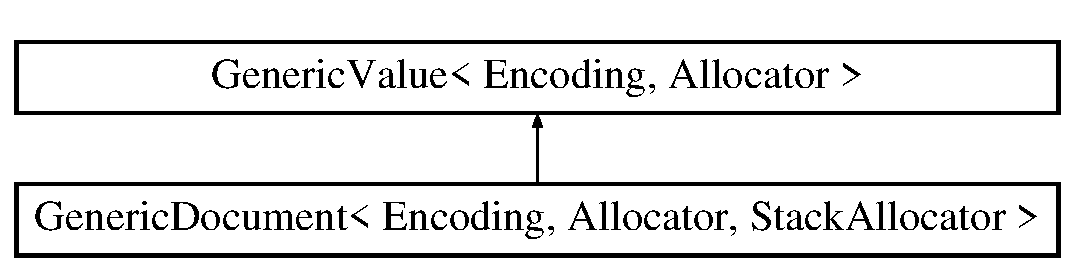
\includegraphics[height=2.000000cm]{a01992}
\end{center}
\end{figure}
\subsection*{Classes}
\begin{DoxyCompactItemize}
\item 
struct \hyperlink{a02112}{Array\+Data}
\item 
union \hyperlink{a02116}{Data}
\item 
struct \hyperlink{a02084}{Flag}
\item 
union \hyperlink{a02096}{Number}
\item 
struct \hyperlink{a02108}{Object\+Data}
\item 
struct \hyperlink{a02092}{Short\+String}
\item 
struct \hyperlink{a02088}{String}
\end{DoxyCompactItemize}
\subsection*{Public Types}
\begin{DoxyCompactItemize}
\item 
\mbox{\Hypertarget{a01992_aa3e89750b19e13a7374c3c0b86b8a113}\label{a01992_aa3e89750b19e13a7374c3c0b86b8a113}} 
enum \{ \newline
{\bfseries k\+Bool\+Flag} = 0x0008, 
{\bfseries k\+Number\+Flag} = 0x0010, 
{\bfseries k\+Int\+Flag} = 0x0020, 
{\bfseries k\+Uint\+Flag} = 0x0040, 
\newline
{\bfseries k\+Int64\+Flag} = 0x0080, 
{\bfseries k\+Uint64\+Flag} = 0x0100, 
{\bfseries k\+Double\+Flag} = 0x0200, 
{\bfseries k\+String\+Flag} = 0x0400, 
\newline
{\bfseries k\+Copy\+Flag} = 0x0800, 
{\bfseries k\+Inline\+Str\+Flag} = 0x1000, 
{\bfseries k\+Null\+Flag} = k\+Null\+Type, 
{\bfseries k\+True\+Flag} = k\+True\+Type $\vert$ k\+Bool\+Flag, 
\newline
{\bfseries k\+False\+Flag} = k\+False\+Type $\vert$ k\+Bool\+Flag, 
{\bfseries k\+Number\+Int\+Flag} = k\+Number\+Type $\vert$ k\+Number\+Flag $\vert$ k\+Int\+Flag $\vert$ k\+Int64\+Flag, 
{\bfseries k\+Number\+Uint\+Flag} = k\+Number\+Type $\vert$ k\+Number\+Flag $\vert$ k\+Uint\+Flag $\vert$ k\+Uint64\+Flag $\vert$ k\+Int64\+Flag, 
{\bfseries k\+Number\+Int64\+Flag} = k\+Number\+Type $\vert$ k\+Number\+Flag $\vert$ k\+Int64\+Flag, 
\newline
{\bfseries k\+Number\+Uint64\+Flag} = k\+Number\+Type $\vert$ k\+Number\+Flag $\vert$ k\+Uint64\+Flag, 
{\bfseries k\+Number\+Double\+Flag} = k\+Number\+Type $\vert$ k\+Number\+Flag $\vert$ k\+Double\+Flag, 
{\bfseries k\+Number\+Any\+Flag} = k\+Number\+Type $\vert$ k\+Number\+Flag $\vert$ k\+Int\+Flag $\vert$ k\+Int64\+Flag $\vert$ k\+Uint\+Flag $\vert$ k\+Uint64\+Flag $\vert$ k\+Double\+Flag, 
{\bfseries k\+Const\+String\+Flag} = k\+String\+Type $\vert$ k\+String\+Flag, 
\newline
{\bfseries k\+Copy\+String\+Flag} = k\+String\+Type $\vert$ k\+String\+Flag $\vert$ k\+Copy\+Flag, 
{\bfseries k\+Short\+String\+Flag} = k\+String\+Type $\vert$ k\+String\+Flag $\vert$ k\+Copy\+Flag $\vert$ k\+Inline\+Str\+Flag, 
{\bfseries k\+Object\+Flag} = k\+Object\+Type, 
{\bfseries k\+Array\+Flag} = k\+Array\+Type, 
\newline
{\bfseries k\+Type\+Mask} = 0x07
 \}
\item 
\mbox{\Hypertarget{a01992_a7ccf27c44058b4c11c3efc6473afb886}\label{a01992_a7ccf27c44058b4c11c3efc6473afb886}} 
typedef \hyperlink{a02000}{Generic\+Member}$<$ Encoding, Allocator $>$ \hyperlink{a01992_a7ccf27c44058b4c11c3efc6473afb886}{Member}
\begin{DoxyCompactList}\small\item\em Name-\/value pair in an object. \end{DoxyCompactList}\item 
\mbox{\Hypertarget{a01992_a28c2cb8d04d12566c1af37597a46d209}\label{a01992_a28c2cb8d04d12566c1af37597a46d209}} 
typedef Encoding \hyperlink{a01992_a28c2cb8d04d12566c1af37597a46d209}{Encoding\+Type}
\begin{DoxyCompactList}\small\item\em Encoding type from template parameter. \end{DoxyCompactList}\item 
\mbox{\Hypertarget{a01992_a7beb83860c1b8d2a0e2a7da9796b2fa1}\label{a01992_a7beb83860c1b8d2a0e2a7da9796b2fa1}} 
typedef Allocator \hyperlink{a01992_a7beb83860c1b8d2a0e2a7da9796b2fa1}{Allocator\+Type}
\begin{DoxyCompactList}\small\item\em Allocator type from template parameter. \end{DoxyCompactList}\item 
\mbox{\Hypertarget{a01992_ade0e0ce64ccd5d852da57a35e720bafb}\label{a01992_ade0e0ce64ccd5d852da57a35e720bafb}} 
typedef Encoding\+::\+Ch \hyperlink{a01992_ade0e0ce64ccd5d852da57a35e720bafb}{Ch}
\begin{DoxyCompactList}\small\item\em Character type derived from Encoding. \end{DoxyCompactList}\item 
\mbox{\Hypertarget{a01992_a32e0f30ee278072374c8168b14d3317f}\label{a01992_a32e0f30ee278072374c8168b14d3317f}} 
typedef \hyperlink{a02008}{Generic\+String\+Ref}$<$ \hyperlink{a01992_ade0e0ce64ccd5d852da57a35e720bafb}{Ch} $>$ \hyperlink{a01992_a32e0f30ee278072374c8168b14d3317f}{String\+Ref\+Type}
\begin{DoxyCompactList}\small\item\em Reference to a constant string. \end{DoxyCompactList}\item 
\mbox{\Hypertarget{a01992_a349b8faae61edc42b4289726820be439}\label{a01992_a349b8faae61edc42b4289726820be439}} 
typedef \hyperlink{a02004}{Generic\+Member\+Iterator}$<$ false, Encoding, Allocator $>$\+::Iterator \hyperlink{a01992_a349b8faae61edc42b4289726820be439}{Member\+Iterator}
\begin{DoxyCompactList}\small\item\em Member iterator for iterating in object. \end{DoxyCompactList}\item 
\mbox{\Hypertarget{a01992_aac08c3e660a9036d3dcb8b10ff6c61f4}\label{a01992_aac08c3e660a9036d3dcb8b10ff6c61f4}} 
typedef \hyperlink{a02004}{Generic\+Member\+Iterator}$<$ true, Encoding, Allocator $>$\+::Iterator \hyperlink{a01992_aac08c3e660a9036d3dcb8b10ff6c61f4}{Const\+Member\+Iterator}
\begin{DoxyCompactList}\small\item\em Constant member iterator for iterating in object. \end{DoxyCompactList}\item 
\mbox{\Hypertarget{a01992_aee30721a49688ba0f865f5d581eb6be9}\label{a01992_aee30721a49688ba0f865f5d581eb6be9}} 
typedef \hyperlink{a01992}{Generic\+Value} $\ast$ \hyperlink{a01992_aee30721a49688ba0f865f5d581eb6be9}{Value\+Iterator}
\begin{DoxyCompactList}\small\item\em Value iterator for iterating in array. \end{DoxyCompactList}\item 
\mbox{\Hypertarget{a01992_a49010c6d6886f96ff0b0c51bccc7f6ea}\label{a01992_a49010c6d6886f96ff0b0c51bccc7f6ea}} 
typedef const \hyperlink{a01992}{Generic\+Value} $\ast$ \hyperlink{a01992_a49010c6d6886f96ff0b0c51bccc7f6ea}{Const\+Value\+Iterator}
\begin{DoxyCompactList}\small\item\em Constant value iterator for iterating in array. \end{DoxyCompactList}\item 
\mbox{\Hypertarget{a01992_a43a39bb4fca9b9d3de3da6ac353d25ce}\label{a01992_a43a39bb4fca9b9d3de3da6ac353d25ce}} 
typedef \hyperlink{a01992}{Generic\+Value}$<$ Encoding, Allocator $>$ \hyperlink{a01992_a43a39bb4fca9b9d3de3da6ac353d25ce}{Value\+Type}
\begin{DoxyCompactList}\small\item\em Value type of itself. \end{DoxyCompactList}\item 
\mbox{\Hypertarget{a01992_a149e12992b8f6064c865a4cf55981b89}\label{a01992_a149e12992b8f6064c865a4cf55981b89}} 
typedef \hyperlink{a02076}{Generic\+Array}$<$ false, \hyperlink{a01992_a43a39bb4fca9b9d3de3da6ac353d25ce}{Value\+Type} $>$ {\bfseries Array}
\item 
\mbox{\Hypertarget{a01992_a8f1d2728de56600b5f3df596e2a8a181}\label{a01992_a8f1d2728de56600b5f3df596e2a8a181}} 
typedef \hyperlink{a02076}{Generic\+Array}$<$ true, \hyperlink{a01992_a43a39bb4fca9b9d3de3da6ac353d25ce}{Value\+Type} $>$ {\bfseries Const\+Array}
\item 
\mbox{\Hypertarget{a01992_aee3606d69d411ce0d98f29639585989b}\label{a01992_aee3606d69d411ce0d98f29639585989b}} 
typedef \hyperlink{a02080}{Generic\+Object}$<$ false, \hyperlink{a01992_a43a39bb4fca9b9d3de3da6ac353d25ce}{Value\+Type} $>$ {\bfseries Object}
\item 
\mbox{\Hypertarget{a01992_a55ad310f5434e0e4a93df616b326ba7e}\label{a01992_a55ad310f5434e0e4a93df616b326ba7e}} 
typedef \hyperlink{a02080}{Generic\+Object}$<$ true, \hyperlink{a01992_a43a39bb4fca9b9d3de3da6ac353d25ce}{Value\+Type} $>$ {\bfseries Const\+Object}
\end{DoxyCompactItemize}
\subsection*{Public Member Functions}
\begin{DoxyCompactItemize}
\item 
{\footnotesize template$<$typename T $>$ }\\\hyperlink{a01992_a4a4418a93777942e1fb7ea71f8aaf680}{R\+A\+P\+I\+D\+J\+S\+O\+N\+\_\+\+D\+I\+S\+A\+B\+L\+E\+I\+F\+\_\+\+R\+E\+T\+U\+RN} ((internal\+::\+Is\+Pointer$<$ T $>$),(\hyperlink{a01992}{Generic\+Value} \&)) operator
\begin{DoxyCompactList}\small\item\em Assignment with primitive types. \end{DoxyCompactList}\item 
\mbox{\Hypertarget{a01992_a0f54466a07c496300b15987e1b1915f8}\label{a01992_a0f54466a07c496300b15987e1b1915f8}} 
R\+A\+P\+I\+D\+J\+S\+O\+N\+\_\+\+F\+O\+R\+C\+E\+I\+N\+L\+I\+NE const \hyperlink{a01992_ade0e0ce64ccd5d852da57a35e720bafb}{Ch} $\ast$ {\bfseries Get\+String\+Pointer} () const
\item 
\mbox{\Hypertarget{a01992_aa3d65011422b4aba50bf035b21a522e1}\label{a01992_aa3d65011422b4aba50bf035b21a522e1}} 
R\+A\+P\+I\+D\+J\+S\+O\+N\+\_\+\+F\+O\+R\+C\+E\+I\+N\+L\+I\+NE const \hyperlink{a01992_ade0e0ce64ccd5d852da57a35e720bafb}{Ch} $\ast$ {\bfseries Set\+String\+Pointer} (const \hyperlink{a01992_ade0e0ce64ccd5d852da57a35e720bafb}{Ch} $\ast$str)
\item 
\mbox{\Hypertarget{a01992_aea7b87806555825ab36ebaaff57440bf}\label{a01992_aea7b87806555825ab36ebaaff57440bf}} 
R\+A\+P\+I\+D\+J\+S\+O\+N\+\_\+\+F\+O\+R\+C\+E\+I\+N\+L\+I\+NE \hyperlink{a01992}{Generic\+Value} $\ast$ {\bfseries Get\+Elements\+Pointer} () const
\item 
\mbox{\Hypertarget{a01992_ad8ac8518160251babea5065f9eea8982}\label{a01992_ad8ac8518160251babea5065f9eea8982}} 
R\+A\+P\+I\+D\+J\+S\+O\+N\+\_\+\+F\+O\+R\+C\+E\+I\+N\+L\+I\+NE \hyperlink{a01992}{Generic\+Value} $\ast$ {\bfseries Set\+Elements\+Pointer} (\hyperlink{a01992}{Generic\+Value} $\ast$elements)
\item 
\mbox{\Hypertarget{a01992_a04412a15687feb103f917cdd91b32298}\label{a01992_a04412a15687feb103f917cdd91b32298}} 
R\+A\+P\+I\+D\+J\+S\+O\+N\+\_\+\+F\+O\+R\+C\+E\+I\+N\+L\+I\+NE \hyperlink{a01992_a7ccf27c44058b4c11c3efc6473afb886}{Member} $\ast$ {\bfseries Get\+Members\+Pointer} () const
\item 
\mbox{\Hypertarget{a01992_a0b488cb0120b154eadde27dc0e694019}\label{a01992_a0b488cb0120b154eadde27dc0e694019}} 
R\+A\+P\+I\+D\+J\+S\+O\+N\+\_\+\+F\+O\+R\+C\+E\+I\+N\+L\+I\+NE \hyperlink{a01992_a7ccf27c44058b4c11c3efc6473afb886}{Member} $\ast$ {\bfseries Set\+Members\+Pointer} (\hyperlink{a01992_a7ccf27c44058b4c11c3efc6473afb886}{Member} $\ast$members)
\item 
\mbox{\Hypertarget{a01992_a8f5f309065479de40a16cf28a340da65}\label{a01992_a8f5f309065479de40a16cf28a340da65}} 
void {\bfseries Set\+Array\+Raw} (\hyperlink{a01992}{Generic\+Value} $\ast$values, \hyperlink{a00560_a5ed6e6e67250fadbd041127e6386dcb5}{Size\+Type} count, Allocator \&allocator)
\item 
\mbox{\Hypertarget{a01992_a26c8ec7d68858df1038506df7fcff22d}\label{a01992_a26c8ec7d68858df1038506df7fcff22d}} 
void \hyperlink{a01992_a26c8ec7d68858df1038506df7fcff22d}{Set\+Object\+Raw} (\hyperlink{a01992_a7ccf27c44058b4c11c3efc6473afb886}{Member} $\ast$members, \hyperlink{a00560_a5ed6e6e67250fadbd041127e6386dcb5}{Size\+Type} count, Allocator \&allocator)
\begin{DoxyCompactList}\small\item\em Initialize this value as object with initial data, without calling destructor. \end{DoxyCompactList}\item 
\mbox{\Hypertarget{a01992_a1451603922dcdf34976f125dc60f70ee}\label{a01992_a1451603922dcdf34976f125dc60f70ee}} 
void \hyperlink{a01992_a1451603922dcdf34976f125dc60f70ee}{Set\+String\+Raw} (\hyperlink{a01992_a32e0f30ee278072374c8168b14d3317f}{String\+Ref\+Type} s) R\+A\+P\+I\+D\+J\+S\+O\+N\+\_\+\+N\+O\+E\+X\+C\+E\+PT
\begin{DoxyCompactList}\small\item\em Initialize this value as constant string, without calling destructor. \end{DoxyCompactList}\item 
\mbox{\Hypertarget{a01992_ad3d91db36dfdbfc1af40a79aae07723c}\label{a01992_ad3d91db36dfdbfc1af40a79aae07723c}} 
void \hyperlink{a01992_ad3d91db36dfdbfc1af40a79aae07723c}{Set\+String\+Raw} (\hyperlink{a01992_a32e0f30ee278072374c8168b14d3317f}{String\+Ref\+Type} s, Allocator \&allocator)
\begin{DoxyCompactList}\small\item\em Initialize this value as copy string with initial data, without calling destructor. \end{DoxyCompactList}\item 
\mbox{\Hypertarget{a01992_abb8ea2dfbe74ff4ee7dac6be31317f81}\label{a01992_abb8ea2dfbe74ff4ee7dac6be31317f81}} 
void \hyperlink{a01992_abb8ea2dfbe74ff4ee7dac6be31317f81}{Raw\+Assign} (\hyperlink{a01992}{Generic\+Value} \&rhs) R\+A\+P\+I\+D\+J\+S\+O\+N\+\_\+\+N\+O\+E\+X\+C\+E\+PT
\begin{DoxyCompactList}\small\item\em Assignment without calling destructor. \end{DoxyCompactList}\item 
\mbox{\Hypertarget{a01992_ad4d088dc601d99fea9d16300a7ec7ee1}\label{a01992_ad4d088dc601d99fea9d16300a7ec7ee1}} 
{\footnotesize template$<$typename Source\+Allocator $>$ }\\bool {\bfseries String\+Equal} (const \hyperlink{a01992}{Generic\+Value}$<$ Encoding, Source\+Allocator $>$ \&rhs) const
\end{DoxyCompactItemize}
\begin{Indent}\textbf{ Assignment operators}\par
\begin{DoxyCompactItemize}
\item 
\hyperlink{a01992}{Generic\+Value} \& \hyperlink{a01992_a9018a40d7c52efc00daf803c51d3236c}{operator=} (\hyperlink{a01992}{Generic\+Value} \&rhs) R\+A\+P\+I\+D\+J\+S\+O\+N\+\_\+\+N\+O\+E\+X\+C\+E\+PT
\begin{DoxyCompactList}\small\item\em Assignment with move semantics. \end{DoxyCompactList}\item 
\hyperlink{a01992}{Generic\+Value} \& \hyperlink{a01992_a386708557555e6389184de608af5e6a6}{operator=} (\hyperlink{a01992_a32e0f30ee278072374c8168b14d3317f}{String\+Ref\+Type} str) R\+A\+P\+I\+D\+J\+S\+O\+N\+\_\+\+N\+O\+E\+X\+C\+E\+PT
\begin{DoxyCompactList}\small\item\em Assignment of constant string reference (no copy) \end{DoxyCompactList}\end{DoxyCompactItemize}
\end{Indent}
\subsection*{Public Attributes}
\begin{DoxyCompactItemize}
\item 
\mbox{\Hypertarget{a01992_aaf80f2c91d26fdde60b9edeeecd3509f}\label{a01992_aaf80f2c91d26fdde60b9edeeecd3509f}} 
\hyperlink{a02116}{Data} {\bfseries data\+\_\+}
\end{DoxyCompactItemize}
\subsection*{Static Public Attributes}
\begin{DoxyCompactItemize}
\item 
\mbox{\Hypertarget{a01992_a188f57bdb1923c1fefe74baa995871a3}\label{a01992_a188f57bdb1923c1fefe74baa995871a3}} 
static const \hyperlink{a00560_a5ed6e6e67250fadbd041127e6386dcb5}{Size\+Type} {\bfseries k\+Default\+Array\+Capacity} = 16
\item 
\mbox{\Hypertarget{a01992_a284d018914629aed9a4bd97fe2dc5899}\label{a01992_a284d018914629aed9a4bd97fe2dc5899}} 
static const \hyperlink{a00560_a5ed6e6e67250fadbd041127e6386dcb5}{Size\+Type} {\bfseries k\+Default\+Object\+Capacity} = 16
\end{DoxyCompactItemize}
\subsection*{Friends}
\begin{DoxyCompactItemize}
\item 
\mbox{\Hypertarget{a01992_ab05bc9e52e201a2867ea5bac141ee1ae}\label{a01992_ab05bc9e52e201a2867ea5bac141ee1ae}} 
{\footnotesize template$<$typename , typename , typename $>$ }\\class {\bfseries Generic\+Document}
\end{DoxyCompactItemize}
\subsection*{Constructors and destructor.}
\begin{DoxyCompactItemize}
\item 
\mbox{\Hypertarget{a01992_ab0205d57176d83814ea4e4598c596fe8}\label{a01992_ab0205d57176d83814ea4e4598c596fe8}} 
\hyperlink{a01992_ab0205d57176d83814ea4e4598c596fe8}{Generic\+Value} () R\+A\+P\+I\+D\+J\+S\+O\+N\+\_\+\+N\+O\+E\+X\+C\+E\+PT
\begin{DoxyCompactList}\small\item\em Default constructor creates a null value. \end{DoxyCompactList}\item 
\hyperlink{a01992_a83c8f84b8e61f2f40414b703b75aea61}{Generic\+Value} (\hyperlink{a00560_a1d1cfd8ffb84e947f82999c682b666a7}{Type} type) R\+A\+P\+I\+D\+J\+S\+O\+N\+\_\+\+N\+O\+E\+X\+C\+E\+PT
\begin{DoxyCompactList}\small\item\em Constructor with J\+S\+ON value type. \end{DoxyCompactList}\item 
{\footnotesize template$<$typename Source\+Allocator $>$ }\\\hyperlink{a01992_a5161c0c98ba9144c50a38acde28a5ede}{Generic\+Value} (const \hyperlink{a01992}{Generic\+Value}$<$ Encoding, Source\+Allocator $>$ \&rhs, Allocator \&allocator)
\begin{DoxyCompactList}\small\item\em Explicit copy constructor (with allocator) \end{DoxyCompactList}\item 
{\footnotesize template$<$typename T $>$ }\\\hyperlink{a01992_a0f6a0394bfffaedde88e433b2265194c}{Generic\+Value} (T b, R\+A\+P\+I\+D\+J\+S\+O\+N\+\_\+\+E\+N\+A\+B\+L\+E\+IF((internal\+::\+Is\+Same$<$ bool, T $>$))) R\+A\+P\+I\+D\+J\+S\+O\+N\+\_\+\+N\+O\+E\+X\+C\+E\+PT
\begin{DoxyCompactList}\small\item\em Constructor for boolean value. \end{DoxyCompactList}\item 
\mbox{\Hypertarget{a01992_aafc754ade38421c179f5c8933ecbaf45}\label{a01992_aafc754ade38421c179f5c8933ecbaf45}} 
\hyperlink{a01992_aafc754ade38421c179f5c8933ecbaf45}{Generic\+Value} (int i) R\+A\+P\+I\+D\+J\+S\+O\+N\+\_\+\+N\+O\+E\+X\+C\+E\+PT
\begin{DoxyCompactList}\small\item\em Constructor for int value. \end{DoxyCompactList}\item 
\mbox{\Hypertarget{a01992_a972bff6c56ac3d04622ff7fad8d98331}\label{a01992_a972bff6c56ac3d04622ff7fad8d98331}} 
\hyperlink{a01992_a972bff6c56ac3d04622ff7fad8d98331}{Generic\+Value} (unsigned u) R\+A\+P\+I\+D\+J\+S\+O\+N\+\_\+\+N\+O\+E\+X\+C\+E\+PT
\begin{DoxyCompactList}\small\item\em Constructor for unsigned value. \end{DoxyCompactList}\item 
\mbox{\Hypertarget{a01992_a964b69f1d2596f75ded5421b6db01a14}\label{a01992_a964b69f1d2596f75ded5421b6db01a14}} 
\hyperlink{a01992_a964b69f1d2596f75ded5421b6db01a14}{Generic\+Value} (int64\+\_\+t i64) R\+A\+P\+I\+D\+J\+S\+O\+N\+\_\+\+N\+O\+E\+X\+C\+E\+PT
\begin{DoxyCompactList}\small\item\em Constructor for int64\+\_\+t value. \end{DoxyCompactList}\item 
\mbox{\Hypertarget{a01992_ad04805a57f5050c8e04be469ba64d6f3}\label{a01992_ad04805a57f5050c8e04be469ba64d6f3}} 
\hyperlink{a01992_ad04805a57f5050c8e04be469ba64d6f3}{Generic\+Value} (uint64\+\_\+t u64) R\+A\+P\+I\+D\+J\+S\+O\+N\+\_\+\+N\+O\+E\+X\+C\+E\+PT
\begin{DoxyCompactList}\small\item\em Constructor for uint64\+\_\+t value. \end{DoxyCompactList}\item 
\mbox{\Hypertarget{a01992_a267d05b7e98c3507908eaf085fe41155}\label{a01992_a267d05b7e98c3507908eaf085fe41155}} 
\hyperlink{a01992_a267d05b7e98c3507908eaf085fe41155}{Generic\+Value} (double d) R\+A\+P\+I\+D\+J\+S\+O\+N\+\_\+\+N\+O\+E\+X\+C\+E\+PT
\begin{DoxyCompactList}\small\item\em Constructor for double value. \end{DoxyCompactList}\item 
\mbox{\Hypertarget{a01992_acad11ab781251634a3c079aa64a6d283}\label{a01992_acad11ab781251634a3c079aa64a6d283}} 
\hyperlink{a01992_acad11ab781251634a3c079aa64a6d283}{Generic\+Value} (float f) R\+A\+P\+I\+D\+J\+S\+O\+N\+\_\+\+N\+O\+E\+X\+C\+E\+PT
\begin{DoxyCompactList}\small\item\em Constructor for float value. \end{DoxyCompactList}\item 
\mbox{\Hypertarget{a01992_a4d9af98141360cd801daab4ed1ca2c91}\label{a01992_a4d9af98141360cd801daab4ed1ca2c91}} 
\hyperlink{a01992_a4d9af98141360cd801daab4ed1ca2c91}{Generic\+Value} (const \hyperlink{a01992_ade0e0ce64ccd5d852da57a35e720bafb}{Ch} $\ast$s, \hyperlink{a00560_a5ed6e6e67250fadbd041127e6386dcb5}{Size\+Type} length) R\+A\+P\+I\+D\+J\+S\+O\+N\+\_\+\+N\+O\+E\+X\+C\+E\+PT
\begin{DoxyCompactList}\small\item\em Constructor for constant string (i.\+e. do not make a copy of string) \end{DoxyCompactList}\item 
\mbox{\Hypertarget{a01992_abb2887958974fef1b2b5c8e32cc72ddb}\label{a01992_abb2887958974fef1b2b5c8e32cc72ddb}} 
\hyperlink{a01992_abb2887958974fef1b2b5c8e32cc72ddb}{Generic\+Value} (\hyperlink{a01992_a32e0f30ee278072374c8168b14d3317f}{String\+Ref\+Type} s) R\+A\+P\+I\+D\+J\+S\+O\+N\+\_\+\+N\+O\+E\+X\+C\+E\+PT
\begin{DoxyCompactList}\small\item\em Constructor for constant string (i.\+e. do not make a copy of string) \end{DoxyCompactList}\item 
\mbox{\Hypertarget{a01992_a9ec2c7cda8c8845acfa3565c6b1b4e10}\label{a01992_a9ec2c7cda8c8845acfa3565c6b1b4e10}} 
\hyperlink{a01992_a9ec2c7cda8c8845acfa3565c6b1b4e10}{Generic\+Value} (const \hyperlink{a01992_ade0e0ce64ccd5d852da57a35e720bafb}{Ch} $\ast$s, \hyperlink{a00560_a5ed6e6e67250fadbd041127e6386dcb5}{Size\+Type} length, Allocator \&allocator)
\begin{DoxyCompactList}\small\item\em Constructor for copy-\/string (i.\+e. do make a copy of string) \end{DoxyCompactList}\item 
\mbox{\Hypertarget{a01992_a9b72b2e3347d4cd77b16c3b45e8decf1}\label{a01992_a9b72b2e3347d4cd77b16c3b45e8decf1}} 
\hyperlink{a01992_a9b72b2e3347d4cd77b16c3b45e8decf1}{Generic\+Value} (const \hyperlink{a01992_ade0e0ce64ccd5d852da57a35e720bafb}{Ch} $\ast$s, Allocator \&allocator)
\begin{DoxyCompactList}\small\item\em Constructor for copy-\/string (i.\+e. do make a copy of string) \end{DoxyCompactList}\item 
\hyperlink{a01992_a953052ef91e54aabe9bdb9f9eaebf6cc}{Generic\+Value} (\hyperlink{a02076}{Array} a) R\+A\+P\+I\+D\+J\+S\+O\+N\+\_\+\+N\+O\+E\+X\+C\+E\+PT
\begin{DoxyCompactList}\small\item\em Constructor for Array. \end{DoxyCompactList}\item 
\hyperlink{a01992_a9c294e56f4ab940f845f7c171b183483}{Generic\+Value} (\hyperlink{a02080}{Object} o) R\+A\+P\+I\+D\+J\+S\+O\+N\+\_\+\+N\+O\+E\+X\+C\+E\+PT
\begin{DoxyCompactList}\small\item\em Constructor for Object. \end{DoxyCompactList}\item 
\hyperlink{a01992_a213ba89ef5ef961a5e655bd8c78ac9f4}{$\sim$\+Generic\+Value} ()
\begin{DoxyCompactList}\small\item\em Destructor. \end{DoxyCompactList}\end{DoxyCompactItemize}


\subsection{Detailed Description}
\subsubsection*{template$<$typename Encoding, typename Allocator = Memory\+Pool\+Allocator$<$$>$$>$\newline
class Generic\+Value$<$ Encoding, Allocator $>$}

Represents a J\+S\+ON value. Use Value for \hyperlink{a02144}{U\+T\+F8} encoding and default allocator. 

A J\+S\+ON value can be one of 7 types. This class is a variant type supporting these types.

Use the Value if \hyperlink{a02144}{U\+T\+F8} and default allocator


\begin{DoxyTemplParams}{Template Parameters}
{\em Encoding} & Encoding of the value. (Even non-\/string values need to have the same encoding in a document) \\
\hline
{\em Allocator} & Allocator type for allocating memory of object, array and string. \\
\hline
\end{DoxyTemplParams}


\subsection{Constructor \& Destructor Documentation}
\mbox{\Hypertarget{a01992_a83c8f84b8e61f2f40414b703b75aea61}\label{a01992_a83c8f84b8e61f2f40414b703b75aea61}} 
\index{Generic\+Value@{Generic\+Value}!Generic\+Value@{Generic\+Value}}
\index{Generic\+Value@{Generic\+Value}!Generic\+Value@{Generic\+Value}}
\subsubsection{\texorpdfstring{Generic\+Value()}{GenericValue()}\hspace{0.1cm}{\footnotesize\ttfamily [1/5]}}
{\footnotesize\ttfamily template$<$typename Encoding, typename Allocator = Memory\+Pool\+Allocator$<$$>$$>$ \\
\hyperlink{a01992}{Generic\+Value}$<$ Encoding, Allocator $>$\+::\hyperlink{a01992}{Generic\+Value} (\begin{DoxyParamCaption}\item[{\hyperlink{a00560_a1d1cfd8ffb84e947f82999c682b666a7}{Type}}]{type }\end{DoxyParamCaption})\hspace{0.3cm}{\ttfamily [inline]}, {\ttfamily [explicit]}}



Constructor with J\+S\+ON value type. 

This creates a Value of specified type with default content. 
\begin{DoxyParams}{Parameters}
{\em type} & Type of the value. \\
\hline
\end{DoxyParams}
\begin{DoxyNote}{Note}
Default content for number is zero. 
\end{DoxyNote}
\mbox{\Hypertarget{a01992_a5161c0c98ba9144c50a38acde28a5ede}\label{a01992_a5161c0c98ba9144c50a38acde28a5ede}} 
\index{Generic\+Value@{Generic\+Value}!Generic\+Value@{Generic\+Value}}
\index{Generic\+Value@{Generic\+Value}!Generic\+Value@{Generic\+Value}}
\subsubsection{\texorpdfstring{Generic\+Value()}{GenericValue()}\hspace{0.1cm}{\footnotesize\ttfamily [2/5]}}
{\footnotesize\ttfamily template$<$typename Encoding, typename Allocator = Memory\+Pool\+Allocator$<$$>$$>$ \\
template$<$typename Source\+Allocator $>$ \\
\hyperlink{a01992}{Generic\+Value}$<$ Encoding, Allocator $>$\+::\hyperlink{a01992}{Generic\+Value} (\begin{DoxyParamCaption}\item[{const \hyperlink{a01992}{Generic\+Value}$<$ Encoding, Source\+Allocator $>$ \&}]{rhs,  }\item[{Allocator \&}]{allocator }\end{DoxyParamCaption})\hspace{0.3cm}{\ttfamily [inline]}}



Explicit copy constructor (with allocator) 

Creates a copy of a Value by using the given Allocator 
\begin{DoxyTemplParams}{Template Parameters}
{\em Source\+Allocator} & allocator of {\ttfamily rhs} \\
\hline
\end{DoxyTemplParams}

\begin{DoxyParams}{Parameters}
{\em rhs} & Value to copy from (read-\/only) \\
\hline
{\em allocator} & Allocator for allocating copied elements and buffers. Commonly use \hyperlink{a01996_aa4609d6b19f86aec1a6b96edf2c27686}{Generic\+Document\+::\+Get\+Allocator()}. \\
\hline
\end{DoxyParams}
\begin{DoxySeeAlso}{See also}
Copy\+From() 
\end{DoxySeeAlso}
\mbox{\Hypertarget{a01992_a0f6a0394bfffaedde88e433b2265194c}\label{a01992_a0f6a0394bfffaedde88e433b2265194c}} 
\index{Generic\+Value@{Generic\+Value}!Generic\+Value@{Generic\+Value}}
\index{Generic\+Value@{Generic\+Value}!Generic\+Value@{Generic\+Value}}
\subsubsection{\texorpdfstring{Generic\+Value()}{GenericValue()}\hspace{0.1cm}{\footnotesize\ttfamily [3/5]}}
{\footnotesize\ttfamily template$<$typename Encoding, typename Allocator = Memory\+Pool\+Allocator$<$$>$$>$ \\
template$<$typename T $>$ \\
\hyperlink{a01992}{Generic\+Value}$<$ Encoding, Allocator $>$\+::\hyperlink{a01992}{Generic\+Value} (\begin{DoxyParamCaption}\item[{T}]{b,  }\item[{R\+A\+P\+I\+D\+J\+S\+O\+N\+\_\+\+E\+N\+A\+B\+L\+E\+IF((internal\+::\+Is\+Same$<$ bool, T $>$))}]{ }\end{DoxyParamCaption})\hspace{0.3cm}{\ttfamily [inline]}, {\ttfamily [explicit]}}



Constructor for boolean value. 


\begin{DoxyParams}{Parameters}
{\em b} & Boolean value \\
\hline
\end{DoxyParams}
\begin{DoxyNote}{Note}
This constructor is limited to {\itshape real} boolean values and rejects implicitly converted types like arbitrary pointers. Use an explicit cast to {\ttfamily bool}, if you want to construct a boolean J\+S\+ON value in such cases. 
\end{DoxyNote}
\mbox{\Hypertarget{a01992_a953052ef91e54aabe9bdb9f9eaebf6cc}\label{a01992_a953052ef91e54aabe9bdb9f9eaebf6cc}} 
\index{Generic\+Value@{Generic\+Value}!Generic\+Value@{Generic\+Value}}
\index{Generic\+Value@{Generic\+Value}!Generic\+Value@{Generic\+Value}}
\subsubsection{\texorpdfstring{Generic\+Value()}{GenericValue()}\hspace{0.1cm}{\footnotesize\ttfamily [4/5]}}
{\footnotesize\ttfamily template$<$typename Encoding, typename Allocator = Memory\+Pool\+Allocator$<$$>$$>$ \\
\hyperlink{a01992}{Generic\+Value}$<$ Encoding, Allocator $>$\+::\hyperlink{a01992}{Generic\+Value} (\begin{DoxyParamCaption}\item[{\hyperlink{a02076}{Array}}]{a }\end{DoxyParamCaption})\hspace{0.3cm}{\ttfamily [inline]}}



Constructor for Array. 


\begin{DoxyParams}{Parameters}
{\em a} & An array obtained by {\ttfamily Get\+Array()}. \\
\hline
\end{DoxyParams}
\begin{DoxyNote}{Note}
{\ttfamily Array} is always pass-\/by-\/value. 

the source array is moved into this value and the sourec array becomes empty. 
\end{DoxyNote}
\mbox{\Hypertarget{a01992_a9c294e56f4ab940f845f7c171b183483}\label{a01992_a9c294e56f4ab940f845f7c171b183483}} 
\index{Generic\+Value@{Generic\+Value}!Generic\+Value@{Generic\+Value}}
\index{Generic\+Value@{Generic\+Value}!Generic\+Value@{Generic\+Value}}
\subsubsection{\texorpdfstring{Generic\+Value()}{GenericValue()}\hspace{0.1cm}{\footnotesize\ttfamily [5/5]}}
{\footnotesize\ttfamily template$<$typename Encoding, typename Allocator = Memory\+Pool\+Allocator$<$$>$$>$ \\
\hyperlink{a01992}{Generic\+Value}$<$ Encoding, Allocator $>$\+::\hyperlink{a01992}{Generic\+Value} (\begin{DoxyParamCaption}\item[{\hyperlink{a02080}{Object}}]{o }\end{DoxyParamCaption})\hspace{0.3cm}{\ttfamily [inline]}}



Constructor for Object. 


\begin{DoxyParams}{Parameters}
{\em o} & An object obtained by {\ttfamily Get\+Object()}. \\
\hline
\end{DoxyParams}
\begin{DoxyNote}{Note}
{\ttfamily Object} is always pass-\/by-\/value. 

the source object is moved into this value and the sourec object becomes empty. 
\end{DoxyNote}
\mbox{\Hypertarget{a01992_a213ba89ef5ef961a5e655bd8c78ac9f4}\label{a01992_a213ba89ef5ef961a5e655bd8c78ac9f4}} 
\index{Generic\+Value@{Generic\+Value}!````~Generic\+Value@{$\sim$\+Generic\+Value}}
\index{````~Generic\+Value@{$\sim$\+Generic\+Value}!Generic\+Value@{Generic\+Value}}
\subsubsection{\texorpdfstring{$\sim$\+Generic\+Value()}{~GenericValue()}}
{\footnotesize\ttfamily template$<$typename Encoding, typename Allocator = Memory\+Pool\+Allocator$<$$>$$>$ \\
\hyperlink{a01992}{Generic\+Value}$<$ Encoding, Allocator $>$\+::$\sim$\hyperlink{a01992}{Generic\+Value} (\begin{DoxyParamCaption}{ }\end{DoxyParamCaption})\hspace{0.3cm}{\ttfamily [inline]}}



Destructor. 

Need to destruct elements of array, members of object, or copy-\/string. 

\subsection{Member Function Documentation}
\mbox{\Hypertarget{a01992_a9018a40d7c52efc00daf803c51d3236c}\label{a01992_a9018a40d7c52efc00daf803c51d3236c}} 
\index{Generic\+Value@{Generic\+Value}!operator=@{operator=}}
\index{operator=@{operator=}!Generic\+Value@{Generic\+Value}}
\subsubsection{\texorpdfstring{operator=()}{operator=()}\hspace{0.1cm}{\footnotesize\ttfamily [1/2]}}
{\footnotesize\ttfamily template$<$typename Encoding, typename Allocator = Memory\+Pool\+Allocator$<$$>$$>$ \\
\hyperlink{a01992}{Generic\+Value}\& \hyperlink{a01992}{Generic\+Value}$<$ Encoding, Allocator $>$\+::operator= (\begin{DoxyParamCaption}\item[{\hyperlink{a01992}{Generic\+Value}$<$ Encoding, Allocator $>$ \&}]{rhs }\end{DoxyParamCaption})\hspace{0.3cm}{\ttfamily [inline]}}



Assignment with move semantics. 


\begin{DoxyParams}{Parameters}
{\em rhs} & Source of the assignment. It will become a null value after assignment. \\
\hline
\end{DoxyParams}
\mbox{\Hypertarget{a01992_a386708557555e6389184de608af5e6a6}\label{a01992_a386708557555e6389184de608af5e6a6}} 
\index{Generic\+Value@{Generic\+Value}!operator=@{operator=}}
\index{operator=@{operator=}!Generic\+Value@{Generic\+Value}}
\subsubsection{\texorpdfstring{operator=()}{operator=()}\hspace{0.1cm}{\footnotesize\ttfamily [2/2]}}
{\footnotesize\ttfamily template$<$typename Encoding, typename Allocator = Memory\+Pool\+Allocator$<$$>$$>$ \\
\hyperlink{a01992}{Generic\+Value}\& \hyperlink{a01992}{Generic\+Value}$<$ Encoding, Allocator $>$\+::operator= (\begin{DoxyParamCaption}\item[{\hyperlink{a01992_a32e0f30ee278072374c8168b14d3317f}{String\+Ref\+Type}}]{str }\end{DoxyParamCaption})\hspace{0.3cm}{\ttfamily [inline]}}



Assignment of constant string reference (no copy) 


\begin{DoxyParams}{Parameters}
{\em str} & Constant string reference to be assigned \\
\hline
\end{DoxyParams}
\begin{DoxyNote}{Note}
This overload is needed to avoid clashes with the generic primitive type assignment overload below. 
\end{DoxyNote}
\begin{DoxySeeAlso}{See also}
\hyperlink{a02008}{Generic\+String\+Ref}, operator=(\+T) 
\end{DoxySeeAlso}
\mbox{\Hypertarget{a01992_a4a4418a93777942e1fb7ea71f8aaf680}\label{a01992_a4a4418a93777942e1fb7ea71f8aaf680}} 
\index{Generic\+Value@{Generic\+Value}!R\+A\+P\+I\+D\+J\+S\+O\+N\+\_\+\+D\+I\+S\+A\+B\+L\+E\+I\+F\+\_\+\+R\+E\+T\+U\+RN@{R\+A\+P\+I\+D\+J\+S\+O\+N\+\_\+\+D\+I\+S\+A\+B\+L\+E\+I\+F\+\_\+\+R\+E\+T\+U\+RN}}
\index{R\+A\+P\+I\+D\+J\+S\+O\+N\+\_\+\+D\+I\+S\+A\+B\+L\+E\+I\+F\+\_\+\+R\+E\+T\+U\+RN@{R\+A\+P\+I\+D\+J\+S\+O\+N\+\_\+\+D\+I\+S\+A\+B\+L\+E\+I\+F\+\_\+\+R\+E\+T\+U\+RN}!Generic\+Value@{Generic\+Value}}
\subsubsection{\texorpdfstring{R\+A\+P\+I\+D\+J\+S\+O\+N\+\_\+\+D\+I\+S\+A\+B\+L\+E\+I\+F\+\_\+\+R\+E\+T\+U\+R\+N()}{RAPIDJSON\_DISABLEIF\_RETURN()}}
{\footnotesize\ttfamily template$<$typename Encoding, typename Allocator = Memory\+Pool\+Allocator$<$$>$$>$ \\
template$<$typename T $>$ \\
\hyperlink{a01992}{Generic\+Value}$<$ Encoding, Allocator $>$\+::R\+A\+P\+I\+D\+J\+S\+O\+N\+\_\+\+D\+I\+S\+A\+B\+L\+E\+I\+F\+\_\+\+R\+E\+T\+U\+RN (\begin{DoxyParamCaption}\item[{(internal\+::\+Is\+Pointer$<$ T $>$)}]{,  }\item[{(\hyperlink{a01992}{Generic\+Value}$<$ Encoding, Allocator $>$ \&)}]{ }\end{DoxyParamCaption})}



Assignment with primitive types. 


\begin{DoxyTemplParams}{Template Parameters}
{\em T} & Either \hyperlink{a00560_a1d1cfd8ffb84e947f82999c682b666a7}{Type}, {\ttfamily int}, {\ttfamily unsigned}, {\ttfamily int64\+\_\+t}, {\ttfamily uint64\+\_\+t} \\
\hline
\end{DoxyTemplParams}

\begin{DoxyParams}{Parameters}
{\em value} & The value to be assigned.\\
\hline
\end{DoxyParams}
\begin{DoxyNote}{Note}
The source type {\ttfamily T} explicitly disallows all pointer types, especially ({\ttfamily const}) \hyperlink{a01992_ade0e0ce64ccd5d852da57a35e720bafb}{Ch}$\ast$. This helps avoiding implicitly referencing character strings with insufficient lifetime, use Set\+String(const Ch$\ast$, Allocator\&) (for copying) or \hyperlink{a00476_aa6b9fd9f6aa49405a574c362ba9af6b5}{String\+Ref()} (to explicitly mark the pointer as constant) instead. All other pointer types would implicitly convert to {\ttfamily bool}, use Set\+Bool() instead.\+Set boolean value 
\end{DoxyNote}


The documentation for this class was generated from the following file\+:\begin{DoxyCompactItemize}
\item 
\hyperlink{a00476}{document.\+h}\end{DoxyCompactItemize}

\hypertarget{a01412}{}\section{boost\+:\+:dll\+:\+:detail\+:\+:get\+\_\+mem\+\_\+fn\+\_\+type$<$ Class, Func $>$ Struct Template Reference}
\label{a01412}\index{boost\+::dll\+::detail\+::get\+\_\+mem\+\_\+fn\+\_\+type$<$ Class, Func $>$@{boost\+::dll\+::detail\+::get\+\_\+mem\+\_\+fn\+\_\+type$<$ Class, Func $>$}}


The documentation for this struct was generated from the following file\+:\begin{DoxyCompactItemize}
\item 
get\+\_\+mem\+\_\+fn\+\_\+type.\+hpp\end{DoxyCompactItemize}

\hypertarget{a01416}{}\section{boost\+:\+:dll\+:\+:detail\+:\+:get\+\_\+mem\+\_\+fn\+\_\+type$<$ Class, Return(Args...)$>$ Struct Template Reference}
\label{a01416}\index{boost\+::dll\+::detail\+::get\+\_\+mem\+\_\+fn\+\_\+type$<$ Class, Return(\+Args...)$>$@{boost\+::dll\+::detail\+::get\+\_\+mem\+\_\+fn\+\_\+type$<$ Class, Return(\+Args...)$>$}}
\subsection*{Public Types}
\begin{DoxyCompactItemize}
\item 
\mbox{\Hypertarget{a01416_a3d6cbb182b6bed192344f19d67769667}\label{a01416_a3d6cbb182b6bed192344f19d67769667}} 
typedef Return(Class\+::$\ast$ {\bfseries mem\+\_\+fn}) (Args...)
\end{DoxyCompactItemize}


The documentation for this struct was generated from the following file\+:\begin{DoxyCompactItemize}
\item 
get\+\_\+mem\+\_\+fn\+\_\+type.\+hpp\end{DoxyCompactItemize}

\hypertarget{a01420}{}\section{boost\+:\+:dll\+:\+:detail\+:\+:get\+\_\+mem\+\_\+fn\+\_\+type$<$ const Class, Return(Args...)$>$ Struct Template Reference}
\label{a01420}\index{boost\+::dll\+::detail\+::get\+\_\+mem\+\_\+fn\+\_\+type$<$ const Class, Return(\+Args...)$>$@{boost\+::dll\+::detail\+::get\+\_\+mem\+\_\+fn\+\_\+type$<$ const Class, Return(\+Args...)$>$}}
\subsection*{Public Types}
\begin{DoxyCompactItemize}
\item 
\mbox{\Hypertarget{a01420_a5959c3f9a01a7442da99eb96b6965673}\label{a01420_a5959c3f9a01a7442da99eb96b6965673}} 
typedef Return(Class\+::$\ast$ {\bfseries mem\+\_\+fn}) (Args...) const
\end{DoxyCompactItemize}


The documentation for this struct was generated from the following file\+:\begin{DoxyCompactItemize}
\item 
get\+\_\+mem\+\_\+fn\+\_\+type.\+hpp\end{DoxyCompactItemize}

\hypertarget{a01428}{}\section{boost\+:\+:dll\+:\+:detail\+:\+:get\+\_\+mem\+\_\+fn\+\_\+type$<$ const volatile Class, Return(Args...)$>$ Struct Template Reference}
\label{a01428}\index{boost\+::dll\+::detail\+::get\+\_\+mem\+\_\+fn\+\_\+type$<$ const volatile Class, Return(\+Args...)$>$@{boost\+::dll\+::detail\+::get\+\_\+mem\+\_\+fn\+\_\+type$<$ const volatile Class, Return(\+Args...)$>$}}
\subsection*{Public Types}
\begin{DoxyCompactItemize}
\item 
\mbox{\Hypertarget{a01428_ab602b8e22e0bf8ce057196dcf8019694}\label{a01428_ab602b8e22e0bf8ce057196dcf8019694}} 
typedef Return(Class\+::$\ast$ {\bfseries mem\+\_\+fn}) (Args...) const volatile
\end{DoxyCompactItemize}


The documentation for this struct was generated from the following file\+:\begin{DoxyCompactItemize}
\item 
get\+\_\+mem\+\_\+fn\+\_\+type.\+hpp\end{DoxyCompactItemize}

\hypertarget{a01424}{}\section{boost\+:\+:dll\+:\+:detail\+:\+:get\+\_\+mem\+\_\+fn\+\_\+type$<$ volatile Class, Return(Args...)$>$ Struct Template Reference}
\label{a01424}\index{boost\+::dll\+::detail\+::get\+\_\+mem\+\_\+fn\+\_\+type$<$ volatile Class, Return(\+Args...)$>$@{boost\+::dll\+::detail\+::get\+\_\+mem\+\_\+fn\+\_\+type$<$ volatile Class, Return(\+Args...)$>$}}
\subsection*{Public Types}
\begin{DoxyCompactItemize}
\item 
\mbox{\Hypertarget{a01424_a2650686f0a64897ada9a29c2f55f8f86}\label{a01424_a2650686f0a64897ada9a29c2f55f8f86}} 
typedef Return(Class\+::$\ast$ {\bfseries mem\+\_\+fn}) (Args...) volatile
\end{DoxyCompactItemize}


The documentation for this struct was generated from the following file\+:\begin{DoxyCompactItemize}
\item 
get\+\_\+mem\+\_\+fn\+\_\+type.\+hpp\end{DoxyCompactItemize}

\hypertarget{a02528}{}\section{xacc\+:\+:Graph$<$ Vertex, type $>$ Class Template Reference}
\label{a02528}\index{xacc\+::\+Graph$<$ Vertex, type $>$@{xacc\+::\+Graph$<$ Vertex, type $>$}}


{\ttfamily \#include $<$Graph.\+hpp$>$}

\subsection*{Classes}
\begin{DoxyCompactItemize}
\item 
class \hyperlink{a02532}{X\+A\+C\+C\+Vertex\+Properties\+Writer}
\end{DoxyCompactItemize}
\subsection*{Public Member Functions}
\begin{DoxyCompactItemize}
\item 
\hyperlink{a02528_a168a916da7346d0af307a75121f80ca4}{Graph} ()
\item 
\hyperlink{a02528_ab513bb56f7a3ede4891aafc586a31717}{Graph} (const int number\+Of\+Vertices)
\item 
void \hyperlink{a02528_a69ddb8cdc899ba47174f0e65b60a75dd}{add\+Edge} (const int src\+Index, const int tgt\+Index, const double edge\+Weight)
\item 
void \hyperlink{a02528_ae9dcc413d7e9b774b6bf2963c261f5fa}{add\+Edge} (const int src\+Index, const int tgt\+Index)
\item 
void \hyperlink{a02528_a99f45a817a10a62dd5f2f8c9a1734d8a}{add\+Vertex} ()
\item 
{\footnotesize template$<$typename ... Properties$>$ }\\void \hyperlink{a02528_a65ccbb34312ab8d6a168f608e10d2b23}{add\+Vertex} (Properties ... properties)
\item 
\mbox{\Hypertarget{a02528_a2eef95bbacd0a7194dea4f81beb1cb37}\label{a02528_a2eef95bbacd0a7194dea4f81beb1cb37}} 
void {\bfseries add\+Vertex} (Vertex \&vertex)
\item 
{\footnotesize template$<$typename... Properties$>$ }\\void \hyperlink{a02528_a26cc1d1d4e1e23b206dcd23b6ef4a8cc}{set\+Vertex\+Properties} (const int index, Properties... properties)
\item 
{\footnotesize template$<$const int Property\+Index$>$ }\\void \hyperlink{a02528_aeeb65835e8a16ebba34da08ea8016fac}{set\+Vertex\+Property} (const int index, decltype(std\+::get$<$ Property\+Index $>$(std\+::declval$<$ Vertex $>$().properties)) prop)
\item 
\mbox{\Hypertarget{a02528_a401589d879abd25f69e38fd197138531}\label{a02528_a401589d879abd25f69e38fd197138531}} 
Vertex \& {\bfseries get\+Vertex} (const int index)
\item 
\mbox{\Hypertarget{a02528_abe1f333b2c9a9f597fb68c00bf44e7f7}\label{a02528_abe1f333b2c9a9f597fb68c00bf44e7f7}} 
auto {\bfseries get\+Vertex\+Properties} (const int index) -\/$>$ decltype(($\ast$\+\_\+graph.\+get())\mbox{[}index\mbox{]}.properties)
\item 
{\footnotesize template$<$const int Property\+Index$>$ }\\decltype(std\+::get$<$ Property\+Index $>$(std\+::declval$<$ Vertex $>$().properties)) \& \hyperlink{a02528_a394f58c21a234393f08b4c3a565a5940}{get\+Vertex\+Property} (const int index)
\item 
void \hyperlink{a02528_aaf1edd0f038f6cca1c3c9ece35d3ec05}{set\+Edge\+Weight} (const int src\+Index, const int tgt\+Index, const double weight)
\item 
double \hyperlink{a02528_a917e439598a91ace852ad67bba029f5c}{get\+Edge\+Weight} (const int src\+Index, const int tgt\+Index)
\item 
bool \hyperlink{a02528_acb5a6e586e58dbef53d84631134a1cdf}{edge\+Exists} (const int src\+Index, const int tgt\+Index)
\item 
int \hyperlink{a02528_afd0f6cc800e0d81f8c168d47c927cf02}{degree} (const int index)
\item 
int \hyperlink{a02528_a9da48591a9d5ec658ae8c62204821ea7}{diameter} ()
\item 
int \hyperlink{a02528_ae3138d390f1d1c7d335144b59df2ddac}{size} ()
\item 
int \hyperlink{a02528_a50fca47e555122b5bb72e93e719484b4}{order} ()
\item 
void \hyperlink{a02528_a56dbba0529135ffdebb4ac3fbdb69252}{write} (std\+::ostream \&stream)
\item 
virtual void \hyperlink{a02528_abdd3e67dc08c223821d809bc8914164a}{read} (std\+::istream \&stream)
\end{DoxyCompactItemize}
\subsection*{Protected Attributes}
\begin{DoxyCompactItemize}
\item 
Boost\+Graph \hyperlink{a02528_acc3a072e3a30cdb8107b571170d96694}{\+\_\+graph}
\end{DoxyCompactItemize}


\subsection{Detailed Description}
\subsubsection*{template$<$typename Vertex, Graph\+Type type = Undirected$>$\newline
class xacc\+::\+Graph$<$ Vertex, type $>$}

The \hyperlink{a02528}{Graph} class provides a generic data structure modeling mathematical graph structures. It is templated on the vertex type, allowing for graphs with a wide variety of graph nodes (for example, in quantum computing -\/ graph of tensors, graph of Ising parameters, etc.)

All provided Vertex types must be a subclass of the Q\+C\+I\+Vertex in order to properly provide a tuple of vertex properties. s 

\subsection{Constructor \& Destructor Documentation}
\mbox{\Hypertarget{a02528_a168a916da7346d0af307a75121f80ca4}\label{a02528_a168a916da7346d0af307a75121f80ca4}} 
\index{xacc\+::\+Graph@{xacc\+::\+Graph}!Graph@{Graph}}
\index{Graph@{Graph}!xacc\+::\+Graph@{xacc\+::\+Graph}}
\subsubsection{\texorpdfstring{Graph()}{Graph()}\hspace{0.1cm}{\footnotesize\ttfamily [1/2]}}
{\footnotesize\ttfamily template$<$typename Vertex, Graph\+Type type = Undirected$>$ \\
\hyperlink{a02528}{xacc\+::\+Graph}$<$ Vertex, type $>$\+::\hyperlink{a02528}{Graph} (\begin{DoxyParamCaption}{ }\end{DoxyParamCaption})\hspace{0.3cm}{\ttfamily [inline]}}

The nullary constructor \mbox{\Hypertarget{a02528_ab513bb56f7a3ede4891aafc586a31717}\label{a02528_ab513bb56f7a3ede4891aafc586a31717}} 
\index{xacc\+::\+Graph@{xacc\+::\+Graph}!Graph@{Graph}}
\index{Graph@{Graph}!xacc\+::\+Graph@{xacc\+::\+Graph}}
\subsubsection{\texorpdfstring{Graph()}{Graph()}\hspace{0.1cm}{\footnotesize\ttfamily [2/2]}}
{\footnotesize\ttfamily template$<$typename Vertex, Graph\+Type type = Undirected$>$ \\
\hyperlink{a02528}{xacc\+::\+Graph}$<$ Vertex, type $>$\+::\hyperlink{a02528}{Graph} (\begin{DoxyParamCaption}\item[{const int}]{number\+Of\+Vertices }\end{DoxyParamCaption})\hspace{0.3cm}{\ttfamily [inline]}}

The constructor, constructs a graph with specified number of vertices.


\begin{DoxyParams}{Parameters}
{\em number\+Of\+Vertices} & The number of vertices \\
\hline
\end{DoxyParams}


\subsection{Member Function Documentation}
\mbox{\Hypertarget{a02528_a69ddb8cdc899ba47174f0e65b60a75dd}\label{a02528_a69ddb8cdc899ba47174f0e65b60a75dd}} 
\index{xacc\+::\+Graph@{xacc\+::\+Graph}!add\+Edge@{add\+Edge}}
\index{add\+Edge@{add\+Edge}!xacc\+::\+Graph@{xacc\+::\+Graph}}
\subsubsection{\texorpdfstring{add\+Edge()}{addEdge()}\hspace{0.1cm}{\footnotesize\ttfamily [1/2]}}
{\footnotesize\ttfamily template$<$typename Vertex, Graph\+Type type = Undirected$>$ \\
void \hyperlink{a02528}{xacc\+::\+Graph}$<$ Vertex, type $>$\+::add\+Edge (\begin{DoxyParamCaption}\item[{const int}]{src\+Index,  }\item[{const int}]{tgt\+Index,  }\item[{const double}]{edge\+Weight }\end{DoxyParamCaption})\hspace{0.3cm}{\ttfamily [inline]}}

Add an edge between the vertices with given provided indices and edge weight.


\begin{DoxyParams}{Parameters}
{\em src\+Index} & Index of the starting vertex \\
\hline
{\em tgt\+Index} & Index of the ending vertex \\
\hline
{\em edge\+Weight} & The edge weight \\
\hline
\end{DoxyParams}
\mbox{\Hypertarget{a02528_ae9dcc413d7e9b774b6bf2963c261f5fa}\label{a02528_ae9dcc413d7e9b774b6bf2963c261f5fa}} 
\index{xacc\+::\+Graph@{xacc\+::\+Graph}!add\+Edge@{add\+Edge}}
\index{add\+Edge@{add\+Edge}!xacc\+::\+Graph@{xacc\+::\+Graph}}
\subsubsection{\texorpdfstring{add\+Edge()}{addEdge()}\hspace{0.1cm}{\footnotesize\ttfamily [2/2]}}
{\footnotesize\ttfamily template$<$typename Vertex, Graph\+Type type = Undirected$>$ \\
void \hyperlink{a02528}{xacc\+::\+Graph}$<$ Vertex, type $>$\+::add\+Edge (\begin{DoxyParamCaption}\item[{const int}]{src\+Index,  }\item[{const int}]{tgt\+Index }\end{DoxyParamCaption})\hspace{0.3cm}{\ttfamily [inline]}}

Add an edge with default edge weight between the vertices at the provided indices.


\begin{DoxyParams}{Parameters}
{\em src\+Index} & Index of the starting vertex \\
\hline
{\em tgt\+Index} & Index of the ending vertex \\
\hline
\end{DoxyParams}
\mbox{\Hypertarget{a02528_a99f45a817a10a62dd5f2f8c9a1734d8a}\label{a02528_a99f45a817a10a62dd5f2f8c9a1734d8a}} 
\index{xacc\+::\+Graph@{xacc\+::\+Graph}!add\+Vertex@{add\+Vertex}}
\index{add\+Vertex@{add\+Vertex}!xacc\+::\+Graph@{xacc\+::\+Graph}}
\subsubsection{\texorpdfstring{add\+Vertex()}{addVertex()}\hspace{0.1cm}{\footnotesize\ttfamily [1/2]}}
{\footnotesize\ttfamily template$<$typename Vertex, Graph\+Type type = Undirected$>$ \\
void \hyperlink{a02528}{xacc\+::\+Graph}$<$ Vertex, type $>$\+::add\+Vertex (\begin{DoxyParamCaption}{ }\end{DoxyParamCaption})\hspace{0.3cm}{\ttfamily [inline]}}

Add a vertex to this \hyperlink{a02528}{Graph}. \mbox{\Hypertarget{a02528_a65ccbb34312ab8d6a168f608e10d2b23}\label{a02528_a65ccbb34312ab8d6a168f608e10d2b23}} 
\index{xacc\+::\+Graph@{xacc\+::\+Graph}!add\+Vertex@{add\+Vertex}}
\index{add\+Vertex@{add\+Vertex}!xacc\+::\+Graph@{xacc\+::\+Graph}}
\subsubsection{\texorpdfstring{add\+Vertex()}{addVertex()}\hspace{0.1cm}{\footnotesize\ttfamily [2/2]}}
{\footnotesize\ttfamily template$<$typename Vertex, Graph\+Type type = Undirected$>$ \\
template$<$typename ... Properties$>$ \\
void \hyperlink{a02528}{xacc\+::\+Graph}$<$ Vertex, type $>$\+::add\+Vertex (\begin{DoxyParamCaption}\item[{Properties ...}]{properties }\end{DoxyParamCaption})\hspace{0.3cm}{\ttfamily [inline]}}

Add a vertex to this graph with the provided properties. s 
\begin{DoxyParams}{Parameters}
{\em properties} & \\
\hline
\end{DoxyParams}
\mbox{\Hypertarget{a02528_afd0f6cc800e0d81f8c168d47c927cf02}\label{a02528_afd0f6cc800e0d81f8c168d47c927cf02}} 
\index{xacc\+::\+Graph@{xacc\+::\+Graph}!degree@{degree}}
\index{degree@{degree}!xacc\+::\+Graph@{xacc\+::\+Graph}}
\subsubsection{\texorpdfstring{degree()}{degree()}}
{\footnotesize\ttfamily template$<$typename Vertex, Graph\+Type type = Undirected$>$ \\
int \hyperlink{a02528}{xacc\+::\+Graph}$<$ Vertex, type $>$\+::degree (\begin{DoxyParamCaption}\item[{const int}]{index }\end{DoxyParamCaption})\hspace{0.3cm}{\ttfamily [inline]}}

Return the vertex degree at the given vertex index.


\begin{DoxyParams}{Parameters}
{\em index} & The index of the vertex \\
\hline
\end{DoxyParams}
\begin{DoxyReturn}{Returns}
degree The degree of the vertex 
\end{DoxyReturn}
\mbox{\Hypertarget{a02528_a9da48591a9d5ec658ae8c62204821ea7}\label{a02528_a9da48591a9d5ec658ae8c62204821ea7}} 
\index{xacc\+::\+Graph@{xacc\+::\+Graph}!diameter@{diameter}}
\index{diameter@{diameter}!xacc\+::\+Graph@{xacc\+::\+Graph}}
\subsubsection{\texorpdfstring{diameter()}{diameter()}}
{\footnotesize\ttfamily template$<$typename Vertex, Graph\+Type type = Undirected$>$ \\
int \hyperlink{a02528}{xacc\+::\+Graph}$<$ Vertex, type $>$\+::diameter (\begin{DoxyParamCaption}{ }\end{DoxyParamCaption})\hspace{0.3cm}{\ttfamily [inline]}}

Return the diameter of this \hyperlink{a02528}{Graph}.

\begin{DoxyReturn}{Returns}
diameter The graph diameter 
\end{DoxyReturn}
\mbox{\Hypertarget{a02528_acb5a6e586e58dbef53d84631134a1cdf}\label{a02528_acb5a6e586e58dbef53d84631134a1cdf}} 
\index{xacc\+::\+Graph@{xacc\+::\+Graph}!edge\+Exists@{edge\+Exists}}
\index{edge\+Exists@{edge\+Exists}!xacc\+::\+Graph@{xacc\+::\+Graph}}
\subsubsection{\texorpdfstring{edge\+Exists()}{edgeExists()}}
{\footnotesize\ttfamily template$<$typename Vertex, Graph\+Type type = Undirected$>$ \\
bool \hyperlink{a02528}{xacc\+::\+Graph}$<$ Vertex, type $>$\+::edge\+Exists (\begin{DoxyParamCaption}\item[{const int}]{src\+Index,  }\item[{const int}]{tgt\+Index }\end{DoxyParamCaption})\hspace{0.3cm}{\ttfamily [inline]}}

Return true if there is an edge between the two vertices at the given vertex indices.


\begin{DoxyParams}{Parameters}
{\em src\+Index} & The starting vertex index \\
\hline
{\em tgt\+Index} & The ending vertex index \\
\hline
\end{DoxyParams}
\begin{DoxyReturn}{Returns}
exists Boolean indicating if edge exists or not 
\end{DoxyReturn}
\mbox{\Hypertarget{a02528_a917e439598a91ace852ad67bba029f5c}\label{a02528_a917e439598a91ace852ad67bba029f5c}} 
\index{xacc\+::\+Graph@{xacc\+::\+Graph}!get\+Edge\+Weight@{get\+Edge\+Weight}}
\index{get\+Edge\+Weight@{get\+Edge\+Weight}!xacc\+::\+Graph@{xacc\+::\+Graph}}
\subsubsection{\texorpdfstring{get\+Edge\+Weight()}{getEdgeWeight()}}
{\footnotesize\ttfamily template$<$typename Vertex, Graph\+Type type = Undirected$>$ \\
double \hyperlink{a02528}{xacc\+::\+Graph}$<$ Vertex, type $>$\+::get\+Edge\+Weight (\begin{DoxyParamCaption}\item[{const int}]{src\+Index,  }\item[{const int}]{tgt\+Index }\end{DoxyParamCaption})\hspace{0.3cm}{\ttfamily [inline]}}

Return the edge weight at the edge between the provided vertices.


\begin{DoxyParams}{Parameters}
{\em src\+Index} & The starting vertex index \\
\hline
{\em tgt\+Index} & The ending vertex index \\
\hline
\end{DoxyParams}
\begin{DoxyReturn}{Returns}
The edge weight 
\end{DoxyReturn}
\mbox{\Hypertarget{a02528_a394f58c21a234393f08b4c3a565a5940}\label{a02528_a394f58c21a234393f08b4c3a565a5940}} 
\index{xacc\+::\+Graph@{xacc\+::\+Graph}!get\+Vertex\+Property@{get\+Vertex\+Property}}
\index{get\+Vertex\+Property@{get\+Vertex\+Property}!xacc\+::\+Graph@{xacc\+::\+Graph}}
\subsubsection{\texorpdfstring{get\+Vertex\+Property()}{getVertexProperty()}}
{\footnotesize\ttfamily template$<$typename Vertex, Graph\+Type type = Undirected$>$ \\
template$<$const int Property\+Index$>$ \\
decltype(std\+::get$<$Property\+Index$>$(std\+::declval$<$Vertex$>$().properties)) \& \hyperlink{a02528}{xacc\+::\+Graph}$<$ Vertex, type $>$\+::get\+Vertex\+Property (\begin{DoxyParamCaption}\item[{const int}]{index }\end{DoxyParamCaption})\hspace{0.3cm}{\ttfamily [inline]}}

Return the vertex property of the vertex at the given index and at the provided valid vertex property template index.


\begin{DoxyParams}{Parameters}
{\em index} & The index of the vertex \\
\hline
\end{DoxyParams}
\begin{DoxyReturn}{Returns}
property The property value. 
\end{DoxyReturn}
\mbox{\Hypertarget{a02528_a50fca47e555122b5bb72e93e719484b4}\label{a02528_a50fca47e555122b5bb72e93e719484b4}} 
\index{xacc\+::\+Graph@{xacc\+::\+Graph}!order@{order}}
\index{order@{order}!xacc\+::\+Graph@{xacc\+::\+Graph}}
\subsubsection{\texorpdfstring{order()}{order()}}
{\footnotesize\ttfamily template$<$typename Vertex, Graph\+Type type = Undirected$>$ \\
int \hyperlink{a02528}{xacc\+::\+Graph}$<$ Vertex, type $>$\+::order (\begin{DoxyParamCaption}{ }\end{DoxyParamCaption})\hspace{0.3cm}{\ttfamily [inline]}}

Return the number of vertices in this graph

\begin{DoxyReturn}{Returns}
n\+Verts The number of vertices. 
\end{DoxyReturn}
\mbox{\Hypertarget{a02528_abdd3e67dc08c223821d809bc8914164a}\label{a02528_abdd3e67dc08c223821d809bc8914164a}} 
\index{xacc\+::\+Graph@{xacc\+::\+Graph}!read@{read}}
\index{read@{read}!xacc\+::\+Graph@{xacc\+::\+Graph}}
\subsubsection{\texorpdfstring{read()}{read()}}
{\footnotesize\ttfamily template$<$typename Vertex, Graph\+Type type = Undirected$>$ \\
virtual void \hyperlink{a02528}{xacc\+::\+Graph}$<$ Vertex, type $>$\+::read (\begin{DoxyParamCaption}\item[{std\+::istream \&}]{stream }\end{DoxyParamCaption})\hspace{0.3cm}{\ttfamily [inline]}, {\ttfamily [virtual]}}

Read in a graphviz dot graph from the given input stream. This is left for subclasses.


\begin{DoxyParams}{Parameters}
{\em stream} & \\
\hline
\end{DoxyParams}


Reimplemented in \hyperlink{a01296_a26019e2f1e13e64645e29aee86ac58b1}{xacc\+::quantum\+::\+Gate\+Q\+IR}, and \hyperlink{a01348_af7a7f4a487d493fe8a4ed1f76cefd731}{xacc\+::quantum\+::\+Quantum\+Circuit}.

\mbox{\Hypertarget{a02528_aaf1edd0f038f6cca1c3c9ece35d3ec05}\label{a02528_aaf1edd0f038f6cca1c3c9ece35d3ec05}} 
\index{xacc\+::\+Graph@{xacc\+::\+Graph}!set\+Edge\+Weight@{set\+Edge\+Weight}}
\index{set\+Edge\+Weight@{set\+Edge\+Weight}!xacc\+::\+Graph@{xacc\+::\+Graph}}
\subsubsection{\texorpdfstring{set\+Edge\+Weight()}{setEdgeWeight()}}
{\footnotesize\ttfamily template$<$typename Vertex, Graph\+Type type = Undirected$>$ \\
void \hyperlink{a02528}{xacc\+::\+Graph}$<$ Vertex, type $>$\+::set\+Edge\+Weight (\begin{DoxyParamCaption}\item[{const int}]{src\+Index,  }\item[{const int}]{tgt\+Index,  }\item[{const double}]{weight }\end{DoxyParamCaption})\hspace{0.3cm}{\ttfamily [inline]}}

Set the weight on the edge between the vertices at the provided indices.


\begin{DoxyParams}{Parameters}
{\em src\+Index} & The starting vertex index \\
\hline
{\em tgt\+Index} & The ending vertex index \\
\hline
{\em weight} & The weight to set. \\
\hline
\end{DoxyParams}
\mbox{\Hypertarget{a02528_a26cc1d1d4e1e23b206dcd23b6ef4a8cc}\label{a02528_a26cc1d1d4e1e23b206dcd23b6ef4a8cc}} 
\index{xacc\+::\+Graph@{xacc\+::\+Graph}!set\+Vertex\+Properties@{set\+Vertex\+Properties}}
\index{set\+Vertex\+Properties@{set\+Vertex\+Properties}!xacc\+::\+Graph@{xacc\+::\+Graph}}
\subsubsection{\texorpdfstring{set\+Vertex\+Properties()}{setVertexProperties()}}
{\footnotesize\ttfamily template$<$typename Vertex, Graph\+Type type = Undirected$>$ \\
template$<$typename... Properties$>$ \\
void \hyperlink{a02528}{xacc\+::\+Graph}$<$ Vertex, type $>$\+::set\+Vertex\+Properties (\begin{DoxyParamCaption}\item[{const int}]{index,  }\item[{Properties...}]{properties }\end{DoxyParamCaption})\hspace{0.3cm}{\ttfamily [inline]}}

Set an existing vertices properties.


\begin{DoxyParams}{Parameters}
{\em index} & The index of the vertex \\
\hline
{\em properties} & The new properties for the vertex \\
\hline
\end{DoxyParams}
\mbox{\Hypertarget{a02528_aeeb65835e8a16ebba34da08ea8016fac}\label{a02528_aeeb65835e8a16ebba34da08ea8016fac}} 
\index{xacc\+::\+Graph@{xacc\+::\+Graph}!set\+Vertex\+Property@{set\+Vertex\+Property}}
\index{set\+Vertex\+Property@{set\+Vertex\+Property}!xacc\+::\+Graph@{xacc\+::\+Graph}}
\subsubsection{\texorpdfstring{set\+Vertex\+Property()}{setVertexProperty()}}
{\footnotesize\ttfamily template$<$typename Vertex, Graph\+Type type = Undirected$>$ \\
template$<$const int Property\+Index$>$ \\
void \hyperlink{a02528}{xacc\+::\+Graph}$<$ Vertex, type $>$\+::set\+Vertex\+Property (\begin{DoxyParamCaption}\item[{const int}]{index,  }\item[{decltype(std\+::get$<$ Property\+Index $>$(std\+::declval$<$ Vertex $>$().properties))}]{prop }\end{DoxyParamCaption})\hspace{0.3cm}{\ttfamily [inline]}}

Set a specific vertex property for the vertex at given index.


\begin{DoxyParams}{Parameters}
{\em index} & The index of the vertex \\
\hline
{\em prop} & The property to set. \\
\hline
\end{DoxyParams}
\mbox{\Hypertarget{a02528_ae3138d390f1d1c7d335144b59df2ddac}\label{a02528_ae3138d390f1d1c7d335144b59df2ddac}} 
\index{xacc\+::\+Graph@{xacc\+::\+Graph}!size@{size}}
\index{size@{size}!xacc\+::\+Graph@{xacc\+::\+Graph}}
\subsubsection{\texorpdfstring{size()}{size()}}
{\footnotesize\ttfamily template$<$typename Vertex, Graph\+Type type = Undirected$>$ \\
int \hyperlink{a02528}{xacc\+::\+Graph}$<$ Vertex, type $>$\+::size (\begin{DoxyParamCaption}{ }\end{DoxyParamCaption})\hspace{0.3cm}{\ttfamily [inline]}}

Return the number of edges. \begin{DoxyReturn}{Returns}
n\+Edges The number of edges. 
\end{DoxyReturn}
\mbox{\Hypertarget{a02528_a56dbba0529135ffdebb4ac3fbdb69252}\label{a02528_a56dbba0529135ffdebb4ac3fbdb69252}} 
\index{xacc\+::\+Graph@{xacc\+::\+Graph}!write@{write}}
\index{write@{write}!xacc\+::\+Graph@{xacc\+::\+Graph}}
\subsubsection{\texorpdfstring{write()}{write()}}
{\footnotesize\ttfamily template$<$typename Vertex, Graph\+Type type = Undirected$>$ \\
void \hyperlink{a02528}{xacc\+::\+Graph}$<$ Vertex, type $>$\+::write (\begin{DoxyParamCaption}\item[{std\+::ostream \&}]{stream }\end{DoxyParamCaption})\hspace{0.3cm}{\ttfamily [inline]}}

Write this graph in a graphviz dot format to the provided ostream.


\begin{DoxyParams}{Parameters}
{\em stream} & \\
\hline
\end{DoxyParams}


\subsection{Member Data Documentation}
\mbox{\Hypertarget{a02528_acc3a072e3a30cdb8107b571170d96694}\label{a02528_acc3a072e3a30cdb8107b571170d96694}} 
\index{xacc\+::\+Graph@{xacc\+::\+Graph}!\+\_\+graph@{\+\_\+graph}}
\index{\+\_\+graph@{\+\_\+graph}!xacc\+::\+Graph@{xacc\+::\+Graph}}
\subsubsection{\texorpdfstring{\+\_\+graph}{\_graph}}
{\footnotesize\ttfamily template$<$typename Vertex, Graph\+Type type = Undirected$>$ \\
Boost\+Graph \hyperlink{a02528}{xacc\+::\+Graph}$<$ Vertex, type $>$\+::\+\_\+graph\hspace{0.3cm}{\ttfamily [protected]}}

The actual graph data structure we are delegating to. 

The documentation for this class was generated from the following file\+:\begin{DoxyCompactItemize}
\item 
Graph.\+hpp\end{DoxyCompactItemize}

\hypertarget{a01308}{}\section{xacc\+:\+:quantum\+:\+:Hadamard Class Reference}
\label{a01308}\index{xacc\+::quantum\+::\+Hadamard@{xacc\+::quantum\+::\+Hadamard}}
Inheritance diagram for xacc\+:\+:quantum\+:\+:Hadamard\+:\begin{figure}[H]
\begin{center}
\leavevmode
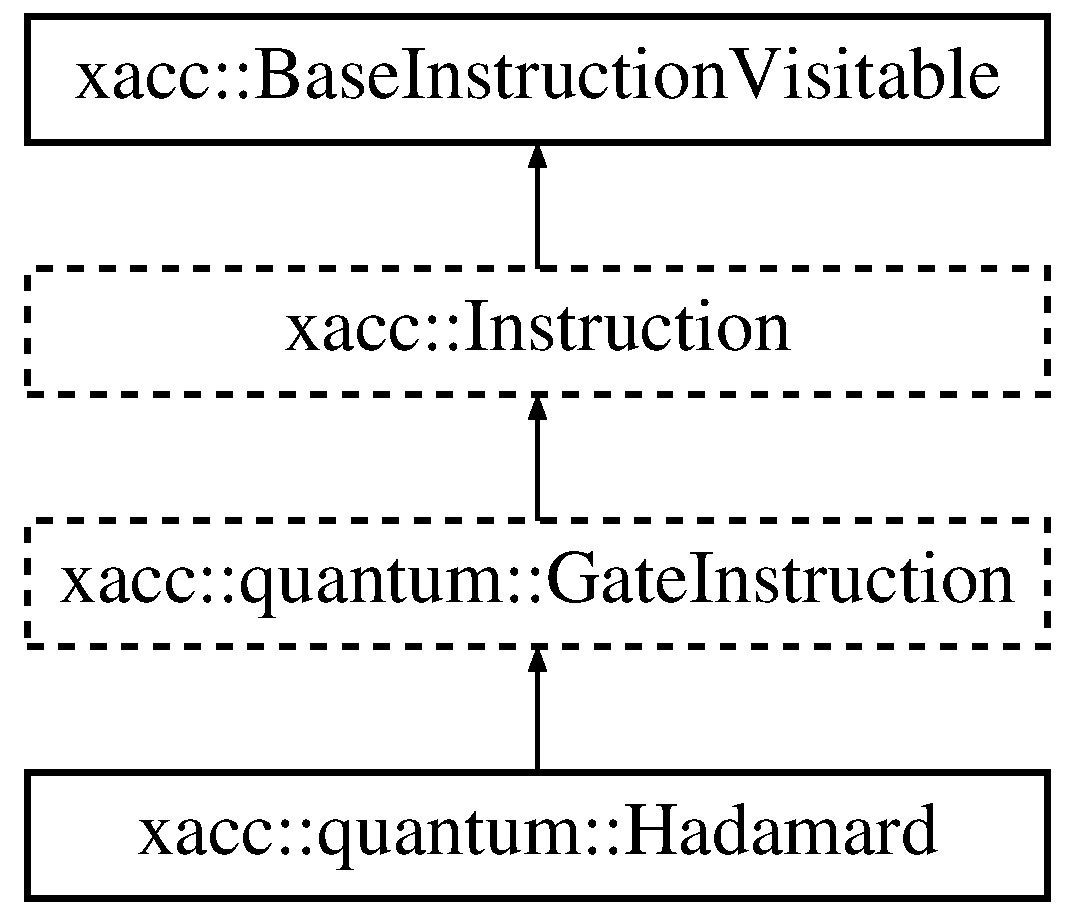
\includegraphics[height=4.000000cm]{a01308}
\end{center}
\end{figure}
\subsection*{Public Member Functions}
\begin{DoxyCompactItemize}
\item 
\mbox{\Hypertarget{a01308_a1f26925eeb4a52ca7e52dd9158fe7005}\label{a01308_a1f26925eeb4a52ca7e52dd9158fe7005}} 
{\bfseries Hadamard} (std\+::vector$<$ int $>$ \hyperlink{a01276_a2a56be6c2519ea65df4d06f4abae1393}{qbits})
\item 
\mbox{\Hypertarget{a01308_aac4e06aae35583bcce39b6b178948364}\label{a01308_aac4e06aae35583bcce39b6b178948364}} 
{\bfseries Hadamard} (int qbit)
\end{DoxyCompactItemize}
\subsection*{Additional Inherited Members}


The documentation for this class was generated from the following files\+:\begin{DoxyCompactItemize}
\item 
Hadamard.\+hpp\item 
Hadamard.\+cpp\end{DoxyCompactItemize}

\hypertarget{a02576}{}\section{rapidjson\+:\+:Handler Class Reference}
\label{a02576}\index{rapidjson\+::\+Handler@{rapidjson\+::\+Handler}}


Concept for receiving events from \hyperlink{a02220}{Generic\+Reader} upon parsing. The functions return true if no error occurs. If they return false, the event publisher should terminate the process.  




{\ttfamily \#include $<$reader.\+h$>$}



\subsection{Detailed Description}
Concept for receiving events from \hyperlink{a02220}{Generic\+Reader} upon parsing. The functions return true if no error occurs. If they return false, the event publisher should terminate the process. 


\begin{DoxyCode}
concept Handler \{
    \textcolor{keyword}{typename} Ch;

    \textcolor{keywordtype}{bool} Null();
    \textcolor{keywordtype}{bool} Bool(\textcolor{keywordtype}{bool} b);
    \textcolor{keywordtype}{bool} Int(\textcolor{keywordtype}{int} i);
    \textcolor{keywordtype}{bool} Uint(\textcolor{keywordtype}{unsigned} i);
    \textcolor{keywordtype}{bool} Int64(int64\_t i);
    \textcolor{keywordtype}{bool} Uint64(uint64\_t i);
    \textcolor{keywordtype}{bool} Double(\textcolor{keywordtype}{double} d);
    \textcolor{keywordtype}{bool} RawNumber(\textcolor{keyword}{const} Ch* str, \hyperlink{a00560_a5ed6e6e67250fadbd041127e6386dcb5}{SizeType} length, \textcolor{keywordtype}{bool} copy);
    \textcolor{keywordtype}{bool} String(\textcolor{keyword}{const} Ch* str, \hyperlink{a00560_a5ed6e6e67250fadbd041127e6386dcb5}{SizeType} length, \textcolor{keywordtype}{bool} copy);
    \textcolor{keywordtype}{bool} StartObject();
    \textcolor{keywordtype}{bool} Key(\textcolor{keyword}{const} Ch* str, \hyperlink{a00560_a5ed6e6e67250fadbd041127e6386dcb5}{SizeType} length, \textcolor{keywordtype}{bool} copy);
    \textcolor{keywordtype}{bool} EndObject(\hyperlink{a00560_a5ed6e6e67250fadbd041127e6386dcb5}{SizeType} memberCount);
    \textcolor{keywordtype}{bool} StartArray();
    \textcolor{keywordtype}{bool} EndArray(\hyperlink{a00560_a5ed6e6e67250fadbd041127e6386dcb5}{SizeType} elementCount);
\};
\end{DoxyCode}
 

The documentation for this class was generated from the following file\+:\begin{DoxyCompactItemize}
\item 
\hyperlink{a00563}{reader.\+h}\end{DoxyCompactItemize}

\hypertarget{a02368}{}\section{internal\+:\+:Hasher$<$ Encoding, Allocator $>$ Class Template Reference}
\label{a02368}\index{internal\+::\+Hasher$<$ Encoding, Allocator $>$@{internal\+::\+Hasher$<$ Encoding, Allocator $>$}}
\subsection*{Public Types}
\begin{DoxyCompactItemize}
\item 
\mbox{\Hypertarget{a02368_a415970af68a067615c3c95306cff6d43}\label{a02368_a415970af68a067615c3c95306cff6d43}} 
typedef Encoding\+::\+Ch {\bfseries Ch}
\end{DoxyCompactItemize}
\subsection*{Public Member Functions}
\begin{DoxyCompactItemize}
\item 
\mbox{\Hypertarget{a02368_a7b6abfdd3bdc60064a2322cdd20708c1}\label{a02368_a7b6abfdd3bdc60064a2322cdd20708c1}} 
{\bfseries Hasher} (Allocator $\ast$allocator=0, size\+\_\+t stack\+Capacity=k\+Default\+Size)
\item 
\mbox{\Hypertarget{a02368_a57c656866aa08cc7c448ce47b7a243c3}\label{a02368_a57c656866aa08cc7c448ce47b7a243c3}} 
bool {\bfseries Null} ()
\item 
\mbox{\Hypertarget{a02368_a11efd784a4e9c4f8a3dc281552df0486}\label{a02368_a11efd784a4e9c4f8a3dc281552df0486}} 
bool {\bfseries Bool} (bool b)
\item 
\mbox{\Hypertarget{a02368_aadbadf98ee7c9ab03a636e0f06d38bac}\label{a02368_aadbadf98ee7c9ab03a636e0f06d38bac}} 
bool {\bfseries Int} (int i)
\item 
\mbox{\Hypertarget{a02368_a4401600c24c817a45cea6c281438e5b4}\label{a02368_a4401600c24c817a45cea6c281438e5b4}} 
bool {\bfseries Uint} (unsigned u)
\item 
\mbox{\Hypertarget{a02368_ae0579cd54b3c545f77452543793b9a97}\label{a02368_ae0579cd54b3c545f77452543793b9a97}} 
bool {\bfseries Int64} (int64\+\_\+t i)
\item 
\mbox{\Hypertarget{a02368_a14832ac4ec204f1065b929df2c255457}\label{a02368_a14832ac4ec204f1065b929df2c255457}} 
bool {\bfseries Uint64} (uint64\+\_\+t u)
\item 
\mbox{\Hypertarget{a02368_a83abe847e24ed88d5aab092d840e37c1}\label{a02368_a83abe847e24ed88d5aab092d840e37c1}} 
bool {\bfseries Double} (double d)
\item 
\mbox{\Hypertarget{a02368_ae277289ad2fb3a938a6507e566d3c5e2}\label{a02368_ae277289ad2fb3a938a6507e566d3c5e2}} 
bool {\bfseries Raw\+Number} (const Ch $\ast$str, \hyperlink{a00560_a5ed6e6e67250fadbd041127e6386dcb5}{Size\+Type} len, bool)
\item 
\mbox{\Hypertarget{a02368_a885f2bf42f2bb64d6f9443129dce3883}\label{a02368_a885f2bf42f2bb64d6f9443129dce3883}} 
bool {\bfseries String} (const Ch $\ast$str, \hyperlink{a00560_a5ed6e6e67250fadbd041127e6386dcb5}{Size\+Type} len, bool)
\item 
\mbox{\Hypertarget{a02368_a1607d6cac3daab9725e442e38d121028}\label{a02368_a1607d6cac3daab9725e442e38d121028}} 
bool {\bfseries Start\+Object} ()
\item 
\mbox{\Hypertarget{a02368_a1b34d88f85f9c6a739c1f9038f14f078}\label{a02368_a1b34d88f85f9c6a739c1f9038f14f078}} 
bool {\bfseries Key} (const Ch $\ast$str, \hyperlink{a00560_a5ed6e6e67250fadbd041127e6386dcb5}{Size\+Type} len, bool copy)
\item 
\mbox{\Hypertarget{a02368_a7050f1552d88967944195163a6a0b08e}\label{a02368_a7050f1552d88967944195163a6a0b08e}} 
bool {\bfseries End\+Object} (\hyperlink{a00560_a5ed6e6e67250fadbd041127e6386dcb5}{Size\+Type} member\+Count)
\item 
\mbox{\Hypertarget{a02368_a2ceb3cc00216f6b6ce66907856a16404}\label{a02368_a2ceb3cc00216f6b6ce66907856a16404}} 
bool {\bfseries Start\+Array} ()
\item 
\mbox{\Hypertarget{a02368_ad445b2730be23e18b4dec2c4d1033419}\label{a02368_ad445b2730be23e18b4dec2c4d1033419}} 
bool {\bfseries End\+Array} (\hyperlink{a00560_a5ed6e6e67250fadbd041127e6386dcb5}{Size\+Type} element\+Count)
\item 
\mbox{\Hypertarget{a02368_ae09fee05c56194031e8af94a1b1be145}\label{a02368_ae09fee05c56194031e8af94a1b1be145}} 
bool {\bfseries Is\+Valid} () const
\item 
\mbox{\Hypertarget{a02368_ac221aaaa0d643aae553125e76aed7b47}\label{a02368_ac221aaaa0d643aae553125e76aed7b47}} 
uint64\+\_\+t {\bfseries Get\+Hash\+Code} () const
\end{DoxyCompactItemize}


The documentation for this class was generated from the following file\+:\begin{DoxyCompactItemize}
\item 
schema.\+h\end{DoxyCompactItemize}

\hypertarget{a02100}{}\section{Generic\+Value$<$ Encoding, Allocator $>$\+:\+:Number\+:\+:I Struct Reference}
\label{a02100}\index{Generic\+Value$<$ Encoding, Allocator $>$\+::\+Number\+::I@{Generic\+Value$<$ Encoding, Allocator $>$\+::\+Number\+::I}}
\subsection*{Public Attributes}
\begin{DoxyCompactItemize}
\item 
\mbox{\Hypertarget{a02100_ae0b250dc448d284cf9019f3932bfc380}\label{a02100_ae0b250dc448d284cf9019f3932bfc380}} 
int {\bfseries i}
\item 
\mbox{\Hypertarget{a02100_aefc064997f30c9c0b2bdce187d1d4cce}\label{a02100_aefc064997f30c9c0b2bdce187d1d4cce}} 
char {\bfseries padding} \mbox{[}4\mbox{]}
\end{DoxyCompactItemize}


The documentation for this struct was generated from the following file\+:\begin{DoxyCompactItemize}
\item 
\hyperlink{a00476}{document.\+h}\end{DoxyCompactItemize}

\hypertarget{a02236}{}\section{I\+Generic\+Remote\+Schema\+Document\+Provider$<$ Schema\+Document\+Type $>$ Class Template Reference}
\label{a02236}\index{I\+Generic\+Remote\+Schema\+Document\+Provider$<$ Schema\+Document\+Type $>$@{I\+Generic\+Remote\+Schema\+Document\+Provider$<$ Schema\+Document\+Type $>$}}
\subsection*{Public Types}
\begin{DoxyCompactItemize}
\item 
\mbox{\Hypertarget{a02236_acfcd5492c3df8ff56cd2d84d36cc0ceb}\label{a02236_acfcd5492c3df8ff56cd2d84d36cc0ceb}} 
typedef Schema\+Document\+Type\+::\+Ch {\bfseries Ch}
\end{DoxyCompactItemize}
\subsection*{Public Member Functions}
\begin{DoxyCompactItemize}
\item 
\mbox{\Hypertarget{a02236_aad112a069dd57fe850fafd04cbb4777b}\label{a02236_aad112a069dd57fe850fafd04cbb4777b}} 
virtual const Schema\+Document\+Type $\ast$ {\bfseries Get\+Remote\+Document} (const Ch $\ast$uri, \hyperlink{a00560_a5ed6e6e67250fadbd041127e6386dcb5}{Size\+Type} length)=0
\end{DoxyCompactItemize}


The documentation for this class was generated from the following files\+:\begin{DoxyCompactItemize}
\item 
fwd.\+h\item 
schema.\+h\end{DoxyCompactItemize}

\hypertarget{a01740}{}\section{fire\+:\+:I\+Local\+Parser$<$ T $>$ Class Template Reference}
\label{a01740}\index{fire\+::\+I\+Local\+Parser$<$ T $>$@{fire\+::\+I\+Local\+Parser$<$ T $>$}}


{\ttfamily \#include $<$I\+Local\+Parser.\+h$>$}

Inheritance diagram for fire\+:\+:I\+Local\+Parser$<$ T $>$\+:\begin{figure}[H]
\begin{center}
\leavevmode
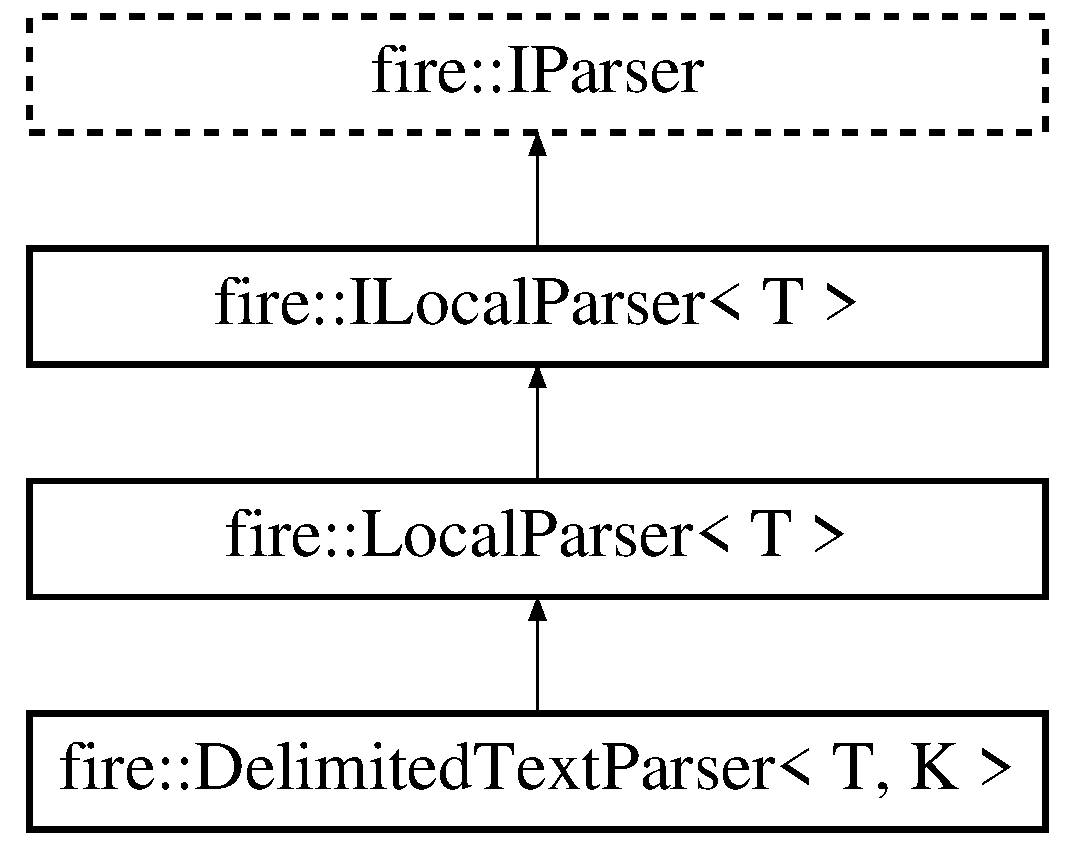
\includegraphics[height=4.000000cm]{a01740}
\end{center}
\end{figure}
\subsection*{Public Member Functions}
\begin{DoxyCompactItemize}
\item 
virtual bool \hyperlink{a01740_a091d5cf56bf8f407854ef87f460b2958}{is\+File} ()
\item 
virtual bool \hyperlink{a01740_a770acae6e216de3a9c7140a12de25d58}{is\+Local} ()
\item 
virtual bool \hyperlink{a01740_ad46898c516adcce38acbb4800dc9777b}{is\+Parallel} ()
\item 
virtual std\+::shared\+\_\+ptr$<$ T $>$ \hyperlink{a01740_a0fc1446d106f0ab8daf8744a4bd29a65}{get\+Data} ()=0
\end{DoxyCompactItemize}
\subsection*{Protected Attributes}
\begin{DoxyCompactItemize}
\item 
bool \hyperlink{a01740_a39adf288ae0bc79cf39fd6e4638858cf}{is\+A\+File} = true
\end{DoxyCompactItemize}


\subsection{Detailed Description}
\subsubsection*{template$<$typename T$>$\newline
class fire\+::\+I\+Local\+Parser$<$ T $>$}

This is a sub-\/interface of \hyperlink{a01748}{I\+Parser} that represents a parser for a local, serially executed parser.

\hyperlink{a01740_a770acae6e216de3a9c7140a12de25d58}{is\+Local()} always returns true. \hyperlink{a01740_ad46898c516adcce38acbb4800dc9777b}{is\+Parallel()} always returns false.

Implementations should set is\+File in their set\+Source(std\+::string) if their source is a file. Subclasses must always be sure that they implement \hyperlink{a01748_af36ac6eedd8c27d2f418869193d7d03c}{parse()} and \hyperlink{a01748_a0dbeff2b9bd8dbfb2aad7a424eef87d1}{set\+Source()} because default implementations are not provided.

The \hyperlink{a01740_a0fc1446d106f0ab8daf8744a4bd29a65}{get\+Data()} operation always returns a shared\+\_\+ptr instead of a raw type (copy) or raw pointer to efficiently share the dynamically allocated data. 

\subsection{Member Function Documentation}
\mbox{\Hypertarget{a01740_a0fc1446d106f0ab8daf8744a4bd29a65}\label{a01740_a0fc1446d106f0ab8daf8744a4bd29a65}} 
\index{fire\+::\+I\+Local\+Parser@{fire\+::\+I\+Local\+Parser}!get\+Data@{get\+Data}}
\index{get\+Data@{get\+Data}!fire\+::\+I\+Local\+Parser@{fire\+::\+I\+Local\+Parser}}
\subsubsection{\texorpdfstring{get\+Data()}{getData()}}
{\footnotesize\ttfamily template$<$typename T$>$ \\
virtual std\+::shared\+\_\+ptr$<$T$>$ \hyperlink{a01740}{fire\+::\+I\+Local\+Parser}$<$ T $>$\+::get\+Data (\begin{DoxyParamCaption}{ }\end{DoxyParamCaption})\hspace{0.3cm}{\ttfamily [pure virtual]}}

This operation returns a shared pointer to an instance of type T. \begin{DoxyReturn}{Returns}
a shared pointer holding an instance of type T that was parsed from the file. 
\end{DoxyReturn}


Implemented in \hyperlink{a01756_ab9016cca8e5dca516bb57c6a8e76607a}{fire\+::\+Local\+Parser$<$ T $>$}, and \hyperlink{a01756_ab9016cca8e5dca516bb57c6a8e76607a}{fire\+::\+Local\+Parser$<$ std\+::string $>$}.

\mbox{\Hypertarget{a01740_a091d5cf56bf8f407854ef87f460b2958}\label{a01740_a091d5cf56bf8f407854ef87f460b2958}} 
\index{fire\+::\+I\+Local\+Parser@{fire\+::\+I\+Local\+Parser}!is\+File@{is\+File}}
\index{is\+File@{is\+File}!fire\+::\+I\+Local\+Parser@{fire\+::\+I\+Local\+Parser}}
\subsubsection{\texorpdfstring{is\+File()}{isFile()}}
{\footnotesize\ttfamily template$<$typename T$>$ \\
virtual bool \hyperlink{a01740}{fire\+::\+I\+Local\+Parser}$<$ T $>$\+::is\+File (\begin{DoxyParamCaption}{ }\end{DoxyParamCaption})\hspace{0.3cm}{\ttfamily [inline]}, {\ttfamily [virtual]}}

This operation indicates whether or not the parser\textquotesingle{}s source is a file. \begin{DoxyReturn}{Returns}
true if this parser is working with a file, false otherwise. 
\end{DoxyReturn}


Implements \hyperlink{a01748_a616c42c85d781c916e97f0ad8f1e9010}{fire\+::\+I\+Parser}.

\mbox{\Hypertarget{a01740_a770acae6e216de3a9c7140a12de25d58}\label{a01740_a770acae6e216de3a9c7140a12de25d58}} 
\index{fire\+::\+I\+Local\+Parser@{fire\+::\+I\+Local\+Parser}!is\+Local@{is\+Local}}
\index{is\+Local@{is\+Local}!fire\+::\+I\+Local\+Parser@{fire\+::\+I\+Local\+Parser}}
\subsubsection{\texorpdfstring{is\+Local()}{isLocal()}}
{\footnotesize\ttfamily template$<$typename T$>$ \\
virtual bool \hyperlink{a01740}{fire\+::\+I\+Local\+Parser}$<$ T $>$\+::is\+Local (\begin{DoxyParamCaption}{ }\end{DoxyParamCaption})\hspace{0.3cm}{\ttfamily [inline]}, {\ttfamily [virtual]}}

This operation indicates whether or not the parser is using a local source. \begin{DoxyReturn}{Returns}
true if this parser is working with a local source, false otherwise. 
\end{DoxyReturn}


Implements \hyperlink{a01748_a97b9e58493b3cadbc63e670b0b0e759f}{fire\+::\+I\+Parser}.

\mbox{\Hypertarget{a01740_ad46898c516adcce38acbb4800dc9777b}\label{a01740_ad46898c516adcce38acbb4800dc9777b}} 
\index{fire\+::\+I\+Local\+Parser@{fire\+::\+I\+Local\+Parser}!is\+Parallel@{is\+Parallel}}
\index{is\+Parallel@{is\+Parallel}!fire\+::\+I\+Local\+Parser@{fire\+::\+I\+Local\+Parser}}
\subsubsection{\texorpdfstring{is\+Parallel()}{isParallel()}}
{\footnotesize\ttfamily template$<$typename T$>$ \\
virtual bool \hyperlink{a01740}{fire\+::\+I\+Local\+Parser}$<$ T $>$\+::is\+Parallel (\begin{DoxyParamCaption}{ }\end{DoxyParamCaption})\hspace{0.3cm}{\ttfamily [inline]}, {\ttfamily [virtual]}}

This operation indicates whether or not the parser reads in parallel. \begin{DoxyReturn}{Returns}
true if this parser reads in parallel, false otherwise. 
\end{DoxyReturn}


Implements \hyperlink{a01748_a83d2882a466d694fb0aea3d846bcbed4}{fire\+::\+I\+Parser}.



\subsection{Member Data Documentation}
\mbox{\Hypertarget{a01740_a39adf288ae0bc79cf39fd6e4638858cf}\label{a01740_a39adf288ae0bc79cf39fd6e4638858cf}} 
\index{fire\+::\+I\+Local\+Parser@{fire\+::\+I\+Local\+Parser}!is\+A\+File@{is\+A\+File}}
\index{is\+A\+File@{is\+A\+File}!fire\+::\+I\+Local\+Parser@{fire\+::\+I\+Local\+Parser}}
\subsubsection{\texorpdfstring{is\+A\+File}{isAFile}}
{\footnotesize\ttfamily template$<$typename T$>$ \\
bool \hyperlink{a01740}{fire\+::\+I\+Local\+Parser}$<$ T $>$\+::is\+A\+File = true\hspace{0.3cm}{\ttfamily [protected]}}

This value is true if the source is a file and false if it is a stream. This value should be set in the set\+Source(std\+::string) and set\+Source(std\+::istream) to true and false respectively. It is set to true by default. 

The documentation for this class was generated from the following file\+:\begin{DoxyCompactItemize}
\item 
I\+Local\+Parser.\+h\end{DoxyCompactItemize}

\hypertarget{a01592}{}\section{boost\+:\+:dll\+:\+:detail\+:\+:I\+M\+A\+G\+E\+\_\+\+D\+A\+T\+A\+\_\+\+D\+I\+R\+E\+C\+T\+O\+R\+Y\+\_\+ Struct Reference}
\label{a01592}\index{boost\+::dll\+::detail\+::\+I\+M\+A\+G\+E\+\_\+\+D\+A\+T\+A\+\_\+\+D\+I\+R\+E\+C\+T\+O\+R\+Y\+\_\+@{boost\+::dll\+::detail\+::\+I\+M\+A\+G\+E\+\_\+\+D\+A\+T\+A\+\_\+\+D\+I\+R\+E\+C\+T\+O\+R\+Y\+\_\+}}
\subsection*{Public Attributes}
\begin{DoxyCompactItemize}
\item 
\mbox{\Hypertarget{a01592_a340957aec7b2353ade198ca79186141e}\label{a01592_a340957aec7b2353ade198ca79186141e}} 
boost\+::dll\+::detail\+::\+D\+W\+O\+R\+D\+\_\+ {\bfseries Virtual\+Address}
\item 
\mbox{\Hypertarget{a01592_a713c3c47477c9d0f55009f8dcfa1bcd0}\label{a01592_a713c3c47477c9d0f55009f8dcfa1bcd0}} 
boost\+::dll\+::detail\+::\+D\+W\+O\+R\+D\+\_\+ {\bfseries Size}
\end{DoxyCompactItemize}


The documentation for this struct was generated from the following file\+:\begin{DoxyCompactItemize}
\item 
pe\+\_\+info.\+hpp\end{DoxyCompactItemize}

\hypertarget{a01584}{}\section{boost\+:\+:dll\+:\+:detail\+:\+:I\+M\+A\+G\+E\+\_\+\+D\+O\+S\+\_\+\+H\+E\+A\+D\+E\+R\+\_\+ Struct Reference}
\label{a01584}\index{boost\+::dll\+::detail\+::\+I\+M\+A\+G\+E\+\_\+\+D\+O\+S\+\_\+\+H\+E\+A\+D\+E\+R\+\_\+@{boost\+::dll\+::detail\+::\+I\+M\+A\+G\+E\+\_\+\+D\+O\+S\+\_\+\+H\+E\+A\+D\+E\+R\+\_\+}}
\subsection*{Public Attributes}
\begin{DoxyCompactItemize}
\item 
\mbox{\Hypertarget{a01584_a3bd0e053bae556df0900f4239d084c3f}\label{a01584_a3bd0e053bae556df0900f4239d084c3f}} 
boost\+::dll\+::detail\+::\+W\+O\+R\+D\+\_\+ {\bfseries e\+\_\+magic}
\item 
\mbox{\Hypertarget{a01584_a841bd5f17ed2800e535b193ea28cbad7}\label{a01584_a841bd5f17ed2800e535b193ea28cbad7}} 
boost\+::dll\+::detail\+::\+W\+O\+R\+D\+\_\+ {\bfseries e\+\_\+cblp}
\item 
\mbox{\Hypertarget{a01584_a87105bdb063d329bff5170ddd0fd7da8}\label{a01584_a87105bdb063d329bff5170ddd0fd7da8}} 
boost\+::dll\+::detail\+::\+W\+O\+R\+D\+\_\+ {\bfseries e\+\_\+cp}
\item 
\mbox{\Hypertarget{a01584_a3e83364e15b65d090ea42acba2462919}\label{a01584_a3e83364e15b65d090ea42acba2462919}} 
boost\+::dll\+::detail\+::\+W\+O\+R\+D\+\_\+ {\bfseries e\+\_\+crlc}
\item 
\mbox{\Hypertarget{a01584_af25651cb91f8a7a7ce62848098ae5f50}\label{a01584_af25651cb91f8a7a7ce62848098ae5f50}} 
boost\+::dll\+::detail\+::\+W\+O\+R\+D\+\_\+ {\bfseries e\+\_\+cparhdr}
\item 
\mbox{\Hypertarget{a01584_adcb216e4dc15485d7d87bceca94d835a}\label{a01584_adcb216e4dc15485d7d87bceca94d835a}} 
boost\+::dll\+::detail\+::\+W\+O\+R\+D\+\_\+ {\bfseries e\+\_\+minalloc}
\item 
\mbox{\Hypertarget{a01584_a66c0ff2d7e1d23973c54e49dfd2e892d}\label{a01584_a66c0ff2d7e1d23973c54e49dfd2e892d}} 
boost\+::dll\+::detail\+::\+W\+O\+R\+D\+\_\+ {\bfseries e\+\_\+maxalloc}
\item 
\mbox{\Hypertarget{a01584_a69354f6406f23c5d1c4bcb5851824cdf}\label{a01584_a69354f6406f23c5d1c4bcb5851824cdf}} 
boost\+::dll\+::detail\+::\+W\+O\+R\+D\+\_\+ {\bfseries e\+\_\+ss}
\item 
\mbox{\Hypertarget{a01584_ab61386ff8426375970baf5ef2f8cf539}\label{a01584_ab61386ff8426375970baf5ef2f8cf539}} 
boost\+::dll\+::detail\+::\+W\+O\+R\+D\+\_\+ {\bfseries e\+\_\+sp}
\item 
\mbox{\Hypertarget{a01584_ad16743e4f83acec334693c2547afb105}\label{a01584_ad16743e4f83acec334693c2547afb105}} 
boost\+::dll\+::detail\+::\+W\+O\+R\+D\+\_\+ {\bfseries e\+\_\+csum}
\item 
\mbox{\Hypertarget{a01584_a8028ae070559f87ec740a03279131eea}\label{a01584_a8028ae070559f87ec740a03279131eea}} 
boost\+::dll\+::detail\+::\+W\+O\+R\+D\+\_\+ {\bfseries e\+\_\+ip}
\item 
\mbox{\Hypertarget{a01584_a919b4a64651b09fedf5e797df7c6f220}\label{a01584_a919b4a64651b09fedf5e797df7c6f220}} 
boost\+::dll\+::detail\+::\+W\+O\+R\+D\+\_\+ {\bfseries e\+\_\+cs}
\item 
\mbox{\Hypertarget{a01584_a9b6f598c4f22bba305e99addb64c2f43}\label{a01584_a9b6f598c4f22bba305e99addb64c2f43}} 
boost\+::dll\+::detail\+::\+W\+O\+R\+D\+\_\+ {\bfseries e\+\_\+lfarlc}
\item 
\mbox{\Hypertarget{a01584_a9aa2f2cf607b90105a03dda7df67f266}\label{a01584_a9aa2f2cf607b90105a03dda7df67f266}} 
boost\+::dll\+::detail\+::\+W\+O\+R\+D\+\_\+ {\bfseries e\+\_\+ovno}
\item 
\mbox{\Hypertarget{a01584_af02a10b7d9dfc56843ebaad25d2e6f2f}\label{a01584_af02a10b7d9dfc56843ebaad25d2e6f2f}} 
boost\+::dll\+::detail\+::\+W\+O\+R\+D\+\_\+ {\bfseries e\+\_\+res} \mbox{[}4\mbox{]}
\item 
\mbox{\Hypertarget{a01584_a5ec6795227f0983da4b2002074731ac6}\label{a01584_a5ec6795227f0983da4b2002074731ac6}} 
boost\+::dll\+::detail\+::\+W\+O\+R\+D\+\_\+ {\bfseries e\+\_\+oemid}
\item 
\mbox{\Hypertarget{a01584_ae0c3c8fa83ec56e89847021b5221971e}\label{a01584_ae0c3c8fa83ec56e89847021b5221971e}} 
boost\+::dll\+::detail\+::\+W\+O\+R\+D\+\_\+ {\bfseries e\+\_\+oeminfo}
\item 
\mbox{\Hypertarget{a01584_a871a5f507eb49fe4977e8759ccc45763}\label{a01584_a871a5f507eb49fe4977e8759ccc45763}} 
boost\+::dll\+::detail\+::\+W\+O\+R\+D\+\_\+ {\bfseries e\+\_\+res2} \mbox{[}10\mbox{]}
\item 
\mbox{\Hypertarget{a01584_a3612d334575e4d09f3f4a11a9ff52e82}\label{a01584_a3612d334575e4d09f3f4a11a9ff52e82}} 
boost\+::dll\+::detail\+::\+L\+O\+N\+G\+\_\+ {\bfseries e\+\_\+lfanew}
\end{DoxyCompactItemize}


The documentation for this struct was generated from the following file\+:\begin{DoxyCompactItemize}
\item 
pe\+\_\+info.\+hpp\end{DoxyCompactItemize}

\hypertarget{a01596}{}\section{boost\+:\+:dll\+:\+:detail\+:\+:I\+M\+A\+G\+E\+\_\+\+E\+X\+P\+O\+R\+T\+\_\+\+D\+I\+R\+E\+C\+T\+O\+R\+Y\+\_\+ Struct Reference}
\label{a01596}\index{boost\+::dll\+::detail\+::\+I\+M\+A\+G\+E\+\_\+\+E\+X\+P\+O\+R\+T\+\_\+\+D\+I\+R\+E\+C\+T\+O\+R\+Y\+\_\+@{boost\+::dll\+::detail\+::\+I\+M\+A\+G\+E\+\_\+\+E\+X\+P\+O\+R\+T\+\_\+\+D\+I\+R\+E\+C\+T\+O\+R\+Y\+\_\+}}
\subsection*{Public Attributes}
\begin{DoxyCompactItemize}
\item 
\mbox{\Hypertarget{a01596_a9e38ab93cca0b67f8e2442732422e6d2}\label{a01596_a9e38ab93cca0b67f8e2442732422e6d2}} 
boost\+::dll\+::detail\+::\+D\+W\+O\+R\+D\+\_\+ {\bfseries Characteristics}
\item 
\mbox{\Hypertarget{a01596_a739de9030de675c85bfeb2a5d3d5be67}\label{a01596_a739de9030de675c85bfeb2a5d3d5be67}} 
boost\+::dll\+::detail\+::\+D\+W\+O\+R\+D\+\_\+ {\bfseries Time\+Date\+Stamp}
\item 
\mbox{\Hypertarget{a01596_a039cfd06d5bb240d9f61dc92eb41f53e}\label{a01596_a039cfd06d5bb240d9f61dc92eb41f53e}} 
boost\+::dll\+::detail\+::\+W\+O\+R\+D\+\_\+ {\bfseries Major\+Version}
\item 
\mbox{\Hypertarget{a01596_a9bba569a6e4fc6ee2f92594cb8b6487f}\label{a01596_a9bba569a6e4fc6ee2f92594cb8b6487f}} 
boost\+::dll\+::detail\+::\+W\+O\+R\+D\+\_\+ {\bfseries Minor\+Version}
\item 
\mbox{\Hypertarget{a01596_ab8e041ceece18fa6e0589eb33d480629}\label{a01596_ab8e041ceece18fa6e0589eb33d480629}} 
boost\+::dll\+::detail\+::\+D\+W\+O\+R\+D\+\_\+ {\bfseries Name}
\item 
\mbox{\Hypertarget{a01596_aec005afc52afc2fab10a60f219a35afc}\label{a01596_aec005afc52afc2fab10a60f219a35afc}} 
boost\+::dll\+::detail\+::\+D\+W\+O\+R\+D\+\_\+ {\bfseries Base}
\item 
\mbox{\Hypertarget{a01596_a7d1acd283af07c583f71f6a5405470fb}\label{a01596_a7d1acd283af07c583f71f6a5405470fb}} 
boost\+::dll\+::detail\+::\+D\+W\+O\+R\+D\+\_\+ {\bfseries Number\+Of\+Functions}
\item 
\mbox{\Hypertarget{a01596_a6fd30ba5be0d6349aa2398a6a4c57eb2}\label{a01596_a6fd30ba5be0d6349aa2398a6a4c57eb2}} 
boost\+::dll\+::detail\+::\+D\+W\+O\+R\+D\+\_\+ {\bfseries Number\+Of\+Names}
\item 
\mbox{\Hypertarget{a01596_a4d24e72a4f88a4c2f6f5205d8cd692a6}\label{a01596_a4d24e72a4f88a4c2f6f5205d8cd692a6}} 
boost\+::dll\+::detail\+::\+D\+W\+O\+R\+D\+\_\+ {\bfseries Address\+Of\+Functions}
\item 
\mbox{\Hypertarget{a01596_a6bcb8739e2a4a7971e0b8586feecbfde}\label{a01596_a6bcb8739e2a4a7971e0b8586feecbfde}} 
boost\+::dll\+::detail\+::\+D\+W\+O\+R\+D\+\_\+ {\bfseries Address\+Of\+Names}
\item 
\mbox{\Hypertarget{a01596_a86a84a8297c28379940f9f748310af8b}\label{a01596_a86a84a8297c28379940f9f748310af8b}} 
boost\+::dll\+::detail\+::\+D\+W\+O\+R\+D\+\_\+ {\bfseries Address\+Of\+Name\+Ordinals}
\end{DoxyCompactItemize}


The documentation for this struct was generated from the following file\+:\begin{DoxyCompactItemize}
\item 
pe\+\_\+info.\+hpp\end{DoxyCompactItemize}

\hypertarget{a01588}{}\section{boost\+:\+:dll\+:\+:detail\+:\+:I\+M\+A\+G\+E\+\_\+\+F\+I\+L\+E\+\_\+\+H\+E\+A\+D\+E\+R\+\_\+ Struct Reference}
\label{a01588}\index{boost\+::dll\+::detail\+::\+I\+M\+A\+G\+E\+\_\+\+F\+I\+L\+E\+\_\+\+H\+E\+A\+D\+E\+R\+\_\+@{boost\+::dll\+::detail\+::\+I\+M\+A\+G\+E\+\_\+\+F\+I\+L\+E\+\_\+\+H\+E\+A\+D\+E\+R\+\_\+}}
\subsection*{Public Attributes}
\begin{DoxyCompactItemize}
\item 
\mbox{\Hypertarget{a01588_a74d0493f559c1790ca07841a9f433d68}\label{a01588_a74d0493f559c1790ca07841a9f433d68}} 
boost\+::dll\+::detail\+::\+W\+O\+R\+D\+\_\+ {\bfseries Machine}
\item 
\mbox{\Hypertarget{a01588_a2e08f6cff4a1d7c7cc4edd0b7376905c}\label{a01588_a2e08f6cff4a1d7c7cc4edd0b7376905c}} 
boost\+::dll\+::detail\+::\+W\+O\+R\+D\+\_\+ {\bfseries Number\+Of\+Sections}
\item 
\mbox{\Hypertarget{a01588_a64d58055b32aa8c8f5e759a7cd7041a0}\label{a01588_a64d58055b32aa8c8f5e759a7cd7041a0}} 
boost\+::dll\+::detail\+::\+D\+W\+O\+R\+D\+\_\+ {\bfseries Time\+Date\+Stamp}
\item 
\mbox{\Hypertarget{a01588_a55b924300db035a900d8acfcb42ed53f}\label{a01588_a55b924300db035a900d8acfcb42ed53f}} 
boost\+::dll\+::detail\+::\+D\+W\+O\+R\+D\+\_\+ {\bfseries Pointer\+To\+Symbol\+Table}
\item 
\mbox{\Hypertarget{a01588_a68ef366c62acd1c494b34f051c3741d9}\label{a01588_a68ef366c62acd1c494b34f051c3741d9}} 
boost\+::dll\+::detail\+::\+D\+W\+O\+R\+D\+\_\+ {\bfseries Number\+Of\+Symbols}
\item 
\mbox{\Hypertarget{a01588_a1faf8ff2d3cd8befadadcf3fbf17c9c2}\label{a01588_a1faf8ff2d3cd8befadadcf3fbf17c9c2}} 
boost\+::dll\+::detail\+::\+W\+O\+R\+D\+\_\+ {\bfseries Size\+Of\+Optional\+Header}
\item 
\mbox{\Hypertarget{a01588_aa0066509ff8a4daf18e369b08880a1b2}\label{a01588_aa0066509ff8a4daf18e369b08880a1b2}} 
boost\+::dll\+::detail\+::\+W\+O\+R\+D\+\_\+ {\bfseries Characteristics}
\end{DoxyCompactItemize}


The documentation for this struct was generated from the following file\+:\begin{DoxyCompactItemize}
\item 
pe\+\_\+info.\+hpp\end{DoxyCompactItemize}

\hypertarget{a01616}{}\section{boost\+:\+:dll\+:\+:detail\+:\+:I\+M\+A\+G\+E\+\_\+\+N\+T\+\_\+\+H\+E\+A\+D\+E\+R\+S\+\_\+template$<$ Address\+OffsetT $>$ Struct Template Reference}
\label{a01616}\index{boost\+::dll\+::detail\+::\+I\+M\+A\+G\+E\+\_\+\+N\+T\+\_\+\+H\+E\+A\+D\+E\+R\+S\+\_\+template$<$ Address\+Offset\+T $>$@{boost\+::dll\+::detail\+::\+I\+M\+A\+G\+E\+\_\+\+N\+T\+\_\+\+H\+E\+A\+D\+E\+R\+S\+\_\+template$<$ Address\+Offset\+T $>$}}
\subsection*{Public Attributes}
\begin{DoxyCompactItemize}
\item 
\mbox{\Hypertarget{a01616_ac62094a288f7e0758fd819727d23d86a}\label{a01616_ac62094a288f7e0758fd819727d23d86a}} 
boost\+::dll\+::detail\+::\+D\+W\+O\+R\+D\+\_\+ {\bfseries Signature}
\item 
\mbox{\Hypertarget{a01616_af79e113f2e6d6dfc51c8310417334b38}\label{a01616_af79e113f2e6d6dfc51c8310417334b38}} 
\hyperlink{a01588}{I\+M\+A\+G\+E\+\_\+\+F\+I\+L\+E\+\_\+\+H\+E\+A\+D\+E\+R\+\_\+} {\bfseries File\+Header}
\item 
\mbox{\Hypertarget{a01616_a11d7a5f9756d15ce28dd47805a89ad0d}\label{a01616_a11d7a5f9756d15ce28dd47805a89ad0d}} 
\hyperlink{a01608}{I\+M\+A\+G\+E\+\_\+\+O\+P\+T\+I\+O\+N\+A\+L\+\_\+\+H\+E\+A\+D\+E\+R\+\_\+template}$<$ Address\+OffsetT $>$ {\bfseries Optional\+Header}
\end{DoxyCompactItemize}


The documentation for this struct was generated from the following file\+:\begin{DoxyCompactItemize}
\item 
pe\+\_\+info.\+hpp\end{DoxyCompactItemize}

\hypertarget{a01608}{}\section{boost\+:\+:dll\+:\+:detail\+:\+:I\+M\+A\+G\+E\+\_\+\+O\+P\+T\+I\+O\+N\+A\+L\+\_\+\+H\+E\+A\+D\+E\+R\+\_\+template$<$ Address\+OffsetT $>$ Struct Template Reference}
\label{a01608}\index{boost\+::dll\+::detail\+::\+I\+M\+A\+G\+E\+\_\+\+O\+P\+T\+I\+O\+N\+A\+L\+\_\+\+H\+E\+A\+D\+E\+R\+\_\+template$<$ Address\+Offset\+T $>$@{boost\+::dll\+::detail\+::\+I\+M\+A\+G\+E\+\_\+\+O\+P\+T\+I\+O\+N\+A\+L\+\_\+\+H\+E\+A\+D\+E\+R\+\_\+template$<$ Address\+Offset\+T $>$}}
\subsection*{Public Attributes}
\begin{DoxyCompactItemize}
\item 
\mbox{\Hypertarget{a01608_acaa65770064417f30dc73e6a3aed5758}\label{a01608_acaa65770064417f30dc73e6a3aed5758}} 
boost\+::dll\+::detail\+::\+W\+O\+R\+D\+\_\+ {\bfseries Magic}
\item 
\mbox{\Hypertarget{a01608_a0ddd4ddd0e85133b67a732a9b5cb50a3}\label{a01608_a0ddd4ddd0e85133b67a732a9b5cb50a3}} 
boost\+::dll\+::detail\+::\+B\+Y\+T\+E\+\_\+ {\bfseries Major\+Linker\+Version}
\item 
\mbox{\Hypertarget{a01608_aac0f854928e88ecddb8671f0992212f9}\label{a01608_aac0f854928e88ecddb8671f0992212f9}} 
boost\+::dll\+::detail\+::\+B\+Y\+T\+E\+\_\+ {\bfseries Minor\+Linker\+Version}
\item 
\mbox{\Hypertarget{a01608_a05f3466faf36daea3c6e3f298ffcb57b}\label{a01608_a05f3466faf36daea3c6e3f298ffcb57b}} 
boost\+::dll\+::detail\+::\+D\+W\+O\+R\+D\+\_\+ {\bfseries Size\+Of\+Code}
\item 
\mbox{\Hypertarget{a01608_a6cdeb05a2e3d8836d60ed324db2a7dfb}\label{a01608_a6cdeb05a2e3d8836d60ed324db2a7dfb}} 
boost\+::dll\+::detail\+::\+D\+W\+O\+R\+D\+\_\+ {\bfseries Size\+Of\+Initialized\+Data}
\item 
\mbox{\Hypertarget{a01608_af9f128f5c560e0922e85840049319b53}\label{a01608_af9f128f5c560e0922e85840049319b53}} 
boost\+::dll\+::detail\+::\+D\+W\+O\+R\+D\+\_\+ {\bfseries Size\+Of\+Uninitialized\+Data}
\item 
\mbox{\Hypertarget{a01608_a58d74a4050edd2858c03cb5c984ac5af}\label{a01608_a58d74a4050edd2858c03cb5c984ac5af}} 
boost\+::dll\+::detail\+::\+D\+W\+O\+R\+D\+\_\+ {\bfseries Address\+Of\+Entry\+Point}
\item 
\mbox{\Hypertarget{a01608_a10b0fad982495fcb899f80f6a96802e8}\label{a01608_a10b0fad982495fcb899f80f6a96802e8}} 
\begin{tabbing}
xx\=xx\=xx\=xx\=xx\=xx\=xx\=xx\=xx\=\kill
union \{\\
\>boost::dll::detail::DWORD\_ {\bfseries BaseOfCode}\\
\>unsigned char {\bfseries padding\_} \mbox{[}sizeof(AddressOffsetT)==8 ? 4 :8\mbox{]}\\
\} {\bfseries BaseOfCode\_and\_BaseOfData}\\

\end{tabbing}\item 
\mbox{\Hypertarget{a01608_aaa98c9194f6cfdc737ea18c5047df18a}\label{a01608_aaa98c9194f6cfdc737ea18c5047df18a}} 
Address\+OffsetT {\bfseries Image\+Base}
\item 
\mbox{\Hypertarget{a01608_a95afdf2ff8a21293d7baad2931e92c15}\label{a01608_a95afdf2ff8a21293d7baad2931e92c15}} 
boost\+::dll\+::detail\+::\+D\+W\+O\+R\+D\+\_\+ {\bfseries Section\+Alignment}
\item 
\mbox{\Hypertarget{a01608_a21fce43504dc1eb8437cf5bd8e04a288}\label{a01608_a21fce43504dc1eb8437cf5bd8e04a288}} 
boost\+::dll\+::detail\+::\+D\+W\+O\+R\+D\+\_\+ {\bfseries File\+Alignment}
\item 
\mbox{\Hypertarget{a01608_a846d83f8a021d3746748d3f6b23a8e45}\label{a01608_a846d83f8a021d3746748d3f6b23a8e45}} 
boost\+::dll\+::detail\+::\+W\+O\+R\+D\+\_\+ {\bfseries Major\+Operating\+System\+Version}
\item 
\mbox{\Hypertarget{a01608_a8a1a7bbb7b06ac2120cfdc09463cd1a7}\label{a01608_a8a1a7bbb7b06ac2120cfdc09463cd1a7}} 
boost\+::dll\+::detail\+::\+W\+O\+R\+D\+\_\+ {\bfseries Minor\+Operating\+System\+Version}
\item 
\mbox{\Hypertarget{a01608_aa237f87b050f32f576c88cb8d2400584}\label{a01608_aa237f87b050f32f576c88cb8d2400584}} 
boost\+::dll\+::detail\+::\+W\+O\+R\+D\+\_\+ {\bfseries Major\+Image\+Version}
\item 
\mbox{\Hypertarget{a01608_a01dd0be3073b05ec638603a048e6f81d}\label{a01608_a01dd0be3073b05ec638603a048e6f81d}} 
boost\+::dll\+::detail\+::\+W\+O\+R\+D\+\_\+ {\bfseries Minor\+Image\+Version}
\item 
\mbox{\Hypertarget{a01608_a6798cbb9208df874e7a93ae809a46ca1}\label{a01608_a6798cbb9208df874e7a93ae809a46ca1}} 
boost\+::dll\+::detail\+::\+W\+O\+R\+D\+\_\+ {\bfseries Major\+Subsystem\+Version}
\item 
\mbox{\Hypertarget{a01608_a56a7cb9654b540992637db37d557220e}\label{a01608_a56a7cb9654b540992637db37d557220e}} 
boost\+::dll\+::detail\+::\+W\+O\+R\+D\+\_\+ {\bfseries Minor\+Subsystem\+Version}
\item 
\mbox{\Hypertarget{a01608_aff33191e6a81cb86fcc6e4b74c35bc02}\label{a01608_aff33191e6a81cb86fcc6e4b74c35bc02}} 
boost\+::dll\+::detail\+::\+D\+W\+O\+R\+D\+\_\+ {\bfseries Win32\+Version\+Value}
\item 
\mbox{\Hypertarget{a01608_a2364a207793f55634d51b18b7d4f902e}\label{a01608_a2364a207793f55634d51b18b7d4f902e}} 
boost\+::dll\+::detail\+::\+D\+W\+O\+R\+D\+\_\+ {\bfseries Size\+Of\+Image}
\item 
\mbox{\Hypertarget{a01608_a77dcf3b10986bd7e1b033d872244cfec}\label{a01608_a77dcf3b10986bd7e1b033d872244cfec}} 
boost\+::dll\+::detail\+::\+D\+W\+O\+R\+D\+\_\+ {\bfseries Size\+Of\+Headers}
\item 
\mbox{\Hypertarget{a01608_a290ac7f032b9881ffffd7bfa46217466}\label{a01608_a290ac7f032b9881ffffd7bfa46217466}} 
boost\+::dll\+::detail\+::\+D\+W\+O\+R\+D\+\_\+ {\bfseries Check\+Sum}
\item 
\mbox{\Hypertarget{a01608_a64a35e14d2ee9b281a3ea11608651764}\label{a01608_a64a35e14d2ee9b281a3ea11608651764}} 
boost\+::dll\+::detail\+::\+W\+O\+R\+D\+\_\+ {\bfseries Subsystem}
\item 
\mbox{\Hypertarget{a01608_ae44cfe64d4300c53e8d5e34851c935fd}\label{a01608_ae44cfe64d4300c53e8d5e34851c935fd}} 
boost\+::dll\+::detail\+::\+W\+O\+R\+D\+\_\+ {\bfseries Dll\+Characteristics}
\item 
\mbox{\Hypertarget{a01608_a2eae163c87c83ceda7a1b3421440170c}\label{a01608_a2eae163c87c83ceda7a1b3421440170c}} 
Address\+OffsetT {\bfseries Size\+Of\+Stack\+Reserve}
\item 
\mbox{\Hypertarget{a01608_a61ac48e1d510e8e16e5de73712cd507a}\label{a01608_a61ac48e1d510e8e16e5de73712cd507a}} 
Address\+OffsetT {\bfseries Size\+Of\+Stack\+Commit}
\item 
\mbox{\Hypertarget{a01608_ace811d417f6d2a48b5f4b036d42474d9}\label{a01608_ace811d417f6d2a48b5f4b036d42474d9}} 
Address\+OffsetT {\bfseries Size\+Of\+Heap\+Reserve}
\item 
\mbox{\Hypertarget{a01608_afb37e14279a636d93b4c748ad5e4c1b1}\label{a01608_afb37e14279a636d93b4c748ad5e4c1b1}} 
Address\+OffsetT {\bfseries Size\+Of\+Heap\+Commit}
\item 
\mbox{\Hypertarget{a01608_a377c1c91e9fe0b9a19297b9689f9dd40}\label{a01608_a377c1c91e9fe0b9a19297b9689f9dd40}} 
boost\+::dll\+::detail\+::\+D\+W\+O\+R\+D\+\_\+ {\bfseries Loader\+Flags}
\item 
\mbox{\Hypertarget{a01608_ad53ec3441a0a0bfe7d5518b2a4a9e0cb}\label{a01608_ad53ec3441a0a0bfe7d5518b2a4a9e0cb}} 
boost\+::dll\+::detail\+::\+D\+W\+O\+R\+D\+\_\+ {\bfseries Number\+Of\+Rva\+And\+Sizes}
\item 
\mbox{\Hypertarget{a01608_a7d7188872466b668272c7daaf937b9dc}\label{a01608_a7d7188872466b668272c7daaf937b9dc}} 
\hyperlink{a01592}{I\+M\+A\+G\+E\+\_\+\+D\+A\+T\+A\+\_\+\+D\+I\+R\+E\+C\+T\+O\+R\+Y\+\_\+} {\bfseries Data\+Directory} \mbox{[}I\+M\+A\+G\+E\+\_\+\+N\+U\+M\+B\+E\+R\+O\+F\+\_\+\+D\+I\+R\+E\+C\+T\+O\+R\+Y\+\_\+\+E\+N\+T\+R\+I\+E\+S\+\_\+\mbox{]}
\end{DoxyCompactItemize}
\subsection*{Static Public Attributes}
\begin{DoxyCompactItemize}
\item 
\mbox{\Hypertarget{a01608_a52f29423206a1a911c33714b2bb547a1}\label{a01608_a52f29423206a1a911c33714b2bb547a1}} 
static const std\+::size\+\_\+t {\bfseries I\+M\+A\+G\+E\+\_\+\+N\+U\+M\+B\+E\+R\+O\+F\+\_\+\+D\+I\+R\+E\+C\+T\+O\+R\+Y\+\_\+\+E\+N\+T\+R\+I\+E\+S\+\_\+} = 16
\end{DoxyCompactItemize}


The documentation for this struct was generated from the following file\+:\begin{DoxyCompactItemize}
\item 
pe\+\_\+info.\+hpp\end{DoxyCompactItemize}

\hypertarget{a01600}{}\section{boost\+:\+:dll\+:\+:detail\+:\+:I\+M\+A\+G\+E\+\_\+\+S\+E\+C\+T\+I\+O\+N\+\_\+\+H\+E\+A\+D\+E\+R\+\_\+ Struct Reference}
\label{a01600}\index{boost\+::dll\+::detail\+::\+I\+M\+A\+G\+E\+\_\+\+S\+E\+C\+T\+I\+O\+N\+\_\+\+H\+E\+A\+D\+E\+R\+\_\+@{boost\+::dll\+::detail\+::\+I\+M\+A\+G\+E\+\_\+\+S\+E\+C\+T\+I\+O\+N\+\_\+\+H\+E\+A\+D\+E\+R\+\_\+}}
\subsection*{Public Attributes}
\begin{DoxyCompactItemize}
\item 
\mbox{\Hypertarget{a01600_aec8a143be7ba929e96b578861cb831a9}\label{a01600_aec8a143be7ba929e96b578861cb831a9}} 
boost\+::dll\+::detail\+::\+B\+Y\+T\+E\+\_\+ {\bfseries Name} \mbox{[}I\+M\+A\+G\+E\+\_\+\+S\+I\+Z\+E\+O\+F\+\_\+\+S\+H\+O\+R\+T\+\_\+\+N\+A\+M\+E\+\_\+\mbox{]}
\item 
\mbox{\Hypertarget{a01600_a57d9142484a367c9aad8bf27d038ba33}\label{a01600_a57d9142484a367c9aad8bf27d038ba33}} 
\begin{tabbing}
xx\=xx\=xx\=xx\=xx\=xx\=xx\=xx\=xx\=\kill
union \{\\
\>boost::dll::detail::DWORD\_ {\bfseries PhysicalAddress}\\
\>boost::dll::detail::DWORD\_ {\bfseries VirtualSize}\\
\} {\bfseries Misc}\\

\end{tabbing}\item 
\mbox{\Hypertarget{a01600_a35eccaade9e46aa496b3dac07499fe39}\label{a01600_a35eccaade9e46aa496b3dac07499fe39}} 
boost\+::dll\+::detail\+::\+D\+W\+O\+R\+D\+\_\+ {\bfseries Virtual\+Address}
\item 
\mbox{\Hypertarget{a01600_afa69e63f2937f44f97ac23666be9d41e}\label{a01600_afa69e63f2937f44f97ac23666be9d41e}} 
boost\+::dll\+::detail\+::\+D\+W\+O\+R\+D\+\_\+ {\bfseries Size\+Of\+Raw\+Data}
\item 
\mbox{\Hypertarget{a01600_ac6df0a4de0101e07e9a7acda52a37e79}\label{a01600_ac6df0a4de0101e07e9a7acda52a37e79}} 
boost\+::dll\+::detail\+::\+D\+W\+O\+R\+D\+\_\+ {\bfseries Pointer\+To\+Raw\+Data}
\item 
\mbox{\Hypertarget{a01600_abd4b898e8d8100a7b9136deaa0a707ed}\label{a01600_abd4b898e8d8100a7b9136deaa0a707ed}} 
boost\+::dll\+::detail\+::\+D\+W\+O\+R\+D\+\_\+ {\bfseries Pointer\+To\+Relocations}
\item 
\mbox{\Hypertarget{a01600_ae07e5d087d87b2c974c2240e588969c9}\label{a01600_ae07e5d087d87b2c974c2240e588969c9}} 
boost\+::dll\+::detail\+::\+D\+W\+O\+R\+D\+\_\+ {\bfseries Pointer\+To\+Linenumbers}
\item 
\mbox{\Hypertarget{a01600_a4ec45186d4ed93d26d49a2be0e91e486}\label{a01600_a4ec45186d4ed93d26d49a2be0e91e486}} 
boost\+::dll\+::detail\+::\+W\+O\+R\+D\+\_\+ {\bfseries Number\+Of\+Relocations}
\item 
\mbox{\Hypertarget{a01600_a1de6e8291c2d0c56d23121a6c7aaaaa3}\label{a01600_a1de6e8291c2d0c56d23121a6c7aaaaa3}} 
boost\+::dll\+::detail\+::\+W\+O\+R\+D\+\_\+ {\bfseries Number\+Of\+Linenumbers}
\item 
\mbox{\Hypertarget{a01600_ac240795840b159ec9fe624eae3969314}\label{a01600_ac240795840b159ec9fe624eae3969314}} 
boost\+::dll\+::detail\+::\+D\+W\+O\+R\+D\+\_\+ {\bfseries Characteristics}
\end{DoxyCompactItemize}
\subsection*{Static Public Attributes}
\begin{DoxyCompactItemize}
\item 
\mbox{\Hypertarget{a01600_ac5eb10907f703acc027687205c5a975f}\label{a01600_ac5eb10907f703acc027687205c5a975f}} 
static const std\+::size\+\_\+t {\bfseries I\+M\+A\+G\+E\+\_\+\+S\+I\+Z\+E\+O\+F\+\_\+\+S\+H\+O\+R\+T\+\_\+\+N\+A\+M\+E\+\_\+} = 8
\end{DoxyCompactItemize}


The documentation for this struct was generated from the following file\+:\begin{DoxyCompactItemize}
\item 
pe\+\_\+info.\+hpp\end{DoxyCompactItemize}

\hypertarget{a02300}{}\section{imaxdiv\+\_\+t Struct Reference}
\label{a02300}\index{imaxdiv\+\_\+t@{imaxdiv\+\_\+t}}
\subsection*{Public Attributes}
\begin{DoxyCompactItemize}
\item 
\mbox{\Hypertarget{a02300_a9339814cbb7610c72fb7d30c6573b393}\label{a02300_a9339814cbb7610c72fb7d30c6573b393}} 
intmax\+\_\+t {\bfseries quot}
\item 
\mbox{\Hypertarget{a02300_a6c9701ad10bff81edae7ff679cae7850}\label{a02300_a6c9701ad10bff81edae7ff679cae7850}} 
intmax\+\_\+t {\bfseries rem}
\end{DoxyCompactItemize}


The documentation for this struct was generated from the following file\+:\begin{DoxyCompactItemize}
\item 
inttypes.\+h\end{DoxyCompactItemize}

\hypertarget{a01636}{}\section{boost\+:\+:dll\+:\+:detail\+:\+:import\+\_\+type$<$ T, class $>$ Struct Template Reference}
\label{a01636}\index{boost\+::dll\+::detail\+::import\+\_\+type$<$ T, class $>$@{boost\+::dll\+::detail\+::import\+\_\+type$<$ T, class $>$}}


The documentation for this struct was generated from the following file\+:\begin{DoxyCompactItemize}
\item 
\hyperlink{a00254}{import.\+hpp}\end{DoxyCompactItemize}

\hypertarget{a01640}{}\section{boost\+:\+:dll\+:\+:detail\+:\+:import\+\_\+type$<$ T, typename boost\+:\+:disable\+\_\+if$<$ boost\+:\+:is\+\_\+object$<$ T $>$ $>$\+:\+:type $>$ Struct Template Reference}
\label{a01640}\index{boost\+::dll\+::detail\+::import\+\_\+type$<$ T, typename boost\+::disable\+\_\+if$<$ boost\+::is\+\_\+object$<$ T $>$ $>$\+::type $>$@{boost\+::dll\+::detail\+::import\+\_\+type$<$ T, typename boost\+::disable\+\_\+if$<$ boost\+::is\+\_\+object$<$ T $>$ $>$\+::type $>$}}
\subsection*{Public Types}
\begin{DoxyCompactItemize}
\item 
\mbox{\Hypertarget{a01640_ac512d41edc93b7e364f66977cc1d51cd}\label{a01640_ac512d41edc93b7e364f66977cc1d51cd}} 
typedef \hyperlink{a01632}{boost\+::dll\+::detail\+::library\+\_\+function}$<$ T $>$ {\bfseries base\+\_\+type}
\item 
\mbox{\Hypertarget{a01640_af0795ef78ae101e0b7f77a18381262e4}\label{a01640_af0795ef78ae101e0b7f77a18381262e4}} 
typedef \hyperlink{a01632}{boost\+::dll\+::detail\+::library\+\_\+function}$<$ T $>$ {\bfseries type}
\end{DoxyCompactItemize}


The documentation for this struct was generated from the following file\+:\begin{DoxyCompactItemize}
\item 
\hyperlink{a00254}{import.\+hpp}\end{DoxyCompactItemize}

\hypertarget{a01644}{}\section{boost\+:\+:dll\+:\+:detail\+:\+:import\+\_\+type$<$ T, typename boost\+:\+:enable\+\_\+if$<$ boost\+:\+:is\+\_\+object$<$ T $>$ $>$\+:\+:type $>$ Struct Template Reference}
\label{a01644}\index{boost\+::dll\+::detail\+::import\+\_\+type$<$ T, typename boost\+::enable\+\_\+if$<$ boost\+::is\+\_\+object$<$ T $>$ $>$\+::type $>$@{boost\+::dll\+::detail\+::import\+\_\+type$<$ T, typename boost\+::enable\+\_\+if$<$ boost\+::is\+\_\+object$<$ T $>$ $>$\+::type $>$}}
\subsection*{Public Types}
\begin{DoxyCompactItemize}
\item 
\mbox{\Hypertarget{a01644_add0253b94384ed45c179b8cac9483401}\label{a01644_add0253b94384ed45c179b8cac9483401}} 
typedef boost\+::shared\+\_\+ptr$<$ T $>$ {\bfseries base\+\_\+type}
\item 
\mbox{\Hypertarget{a01644_abfa036f322955328a8fe74db901065ba}\label{a01644_abfa036f322955328a8fe74db901065ba}} 
typedef boost\+::shared\+\_\+ptr$<$ T $>$ {\bfseries type}
\end{DoxyCompactItemize}


The documentation for this struct was generated from the following file\+:\begin{DoxyCompactItemize}
\item 
\hyperlink{a00254}{import.\+hpp}\end{DoxyCompactItemize}

\hypertarget{a01664}{}\section{boost\+:\+:dll\+:\+:experimental\+:\+:imported\+\_\+class$<$ T $>$ Class Template Reference}
\label{a01664}\index{boost\+::dll\+::experimental\+::imported\+\_\+class$<$ T $>$@{boost\+::dll\+::experimental\+::imported\+\_\+class$<$ T $>$}}


{\ttfamily \#include $<$import\+\_\+class.\+hpp$>$}

\subsection*{Public Types}
\begin{DoxyCompactItemize}
\item 
\mbox{\Hypertarget{a01664_acc2cfce842c9bac2feccb2a601f8bdc7}\label{a01664_acc2cfce842c9bac2feccb2a601f8bdc7}} 
typedef \hyperlink{a01664}{imported\+\_\+class}$<$ T $>$ {\bfseries base\+\_\+t}
\end{DoxyCompactItemize}
\subsection*{Public Member Functions}
\begin{DoxyCompactItemize}
\item 
\mbox{\Hypertarget{a01664_a6605491bba4a2f25af7d7dbb86855524}\label{a01664_a6605491bba4a2f25af7d7dbb86855524}} 
T $\ast$ \hyperlink{a01664_a6605491bba4a2f25af7d7dbb86855524}{get} ()
\begin{DoxyCompactList}\small\item\em Returns a pointer to the underlying class. \end{DoxyCompactList}\item 
\mbox{\Hypertarget{a01664_adf0748e828a8fc810b721b017735dbbb}\label{a01664_adf0748e828a8fc810b721b017735dbbb}} 
{\bfseries imported\+\_\+class} (\hyperlink{a01664}{imported\+\_\+class} \&)=delete
\item 
\mbox{\Hypertarget{a01664_abdd658355cf8bdd782138525420a794c}\label{a01664_abdd658355cf8bdd782138525420a794c}} 
\hyperlink{a01664_abdd658355cf8bdd782138525420a794c}{imported\+\_\+class} (\hyperlink{a01664}{imported\+\_\+class} \&\&)=default
\begin{DoxyCompactList}\small\item\em Move constructor. \end{DoxyCompactList}\item 
\mbox{\Hypertarget{a01664_a100fea6a169061c64a84d584c81f947f}\label{a01664_a100fea6a169061c64a84d584c81f947f}} 
\hyperlink{a01664}{imported\+\_\+class} \& {\bfseries operator=} (\hyperlink{a01664}{imported\+\_\+class} \&)=delete
\item 
\mbox{\Hypertarget{a01664_a0a3936704be3249f7bce69e24e230626}\label{a01664_a0a3936704be3249f7bce69e24e230626}} 
\hyperlink{a01664}{imported\+\_\+class} \& \hyperlink{a01664_a0a3936704be3249f7bce69e24e230626}{operator=} (\hyperlink{a01664}{imported\+\_\+class} \&\&)=default
\begin{DoxyCompactList}\small\item\em Move assignmend. \end{DoxyCompactList}\item 
\mbox{\Hypertarget{a01664_a8609448b6dc64a623863793d6dedde75}\label{a01664_a8609448b6dc64a623863793d6dedde75}} 
bool \hyperlink{a01664_a8609448b6dc64a623863793d6dedde75}{is\+\_\+move\+\_\+constructible} ()
\begin{DoxyCompactList}\small\item\em Check if the imported class is move-\/constructible. \end{DoxyCompactList}\item 
\mbox{\Hypertarget{a01664_ac0c08ef84b2659240001af9f346e7d85}\label{a01664_ac0c08ef84b2659240001af9f346e7d85}} 
bool \hyperlink{a01664_ac0c08ef84b2659240001af9f346e7d85}{is\+\_\+move\+\_\+assignable} ()
\begin{DoxyCompactList}\small\item\em Check if the imported class is move-\/assignable. \end{DoxyCompactList}\item 
\mbox{\Hypertarget{a01664_a8a6beccfbcee584e8cc4c6ee1989e4ce}\label{a01664_a8a6beccfbcee584e8cc4c6ee1989e4ce}} 
bool \hyperlink{a01664_a8a6beccfbcee584e8cc4c6ee1989e4ce}{is\+\_\+copy\+\_\+constructible} ()
\begin{DoxyCompactList}\small\item\em Check if the imported class is copy-\/constructible. \end{DoxyCompactList}\item 
\mbox{\Hypertarget{a01664_a00a39e705beafb32b8e37d704437e251}\label{a01664_a00a39e705beafb32b8e37d704437e251}} 
bool \hyperlink{a01664_a00a39e705beafb32b8e37d704437e251}{is\+\_\+copy\+\_\+assignable} ()
\begin{DoxyCompactList}\small\item\em Check if the imported class is copy-\/assignable. \end{DoxyCompactList}\item 
\hyperlink{a01664}{imported\+\_\+class}$<$ T $>$ \hyperlink{a01664_a382c085143f6c91b0d0a52dd1cb7851a}{copy} () const
\begin{DoxyCompactList}\small\item\em Invoke the copy constructor. \end{DoxyCompactList}\item 
\hyperlink{a01664}{imported\+\_\+class}$<$ T $>$ \hyperlink{a01664_a081d37ced4c6ac2b130d353dac432854}{move} ()
\begin{DoxyCompactList}\small\item\em Invoke the move constructor. \end{DoxyCompactList}\item 
void \hyperlink{a01664_aabf3d4c96c020a756b73db59dfbf46ba}{copy\+\_\+assign} (const \hyperlink{a01664}{imported\+\_\+class}$<$ T $>$ \&lhs) const
\begin{DoxyCompactList}\small\item\em Invoke the copy assignment. \end{DoxyCompactList}\item 
void \hyperlink{a01664_a0e6112cf988cbe0a2b05e0d5dc874a66}{move\+\_\+assign} (\hyperlink{a01664}{imported\+\_\+class}$<$ T $>$ \&lhs)
\begin{DoxyCompactList}\small\item\em Invoke the move assignment. \end{DoxyCompactList}\item 
\mbox{\Hypertarget{a01664_aa1c582893dd221ef1df729931d6aa2bf}\label{a01664_aa1c582893dd221ef1df729931d6aa2bf}} 
\hyperlink{a01664_aa1c582893dd221ef1df729931d6aa2bf}{operator bool} () const
\begin{DoxyCompactList}\small\item\em Check if the class is loaded. \end{DoxyCompactList}\item 
\mbox{\Hypertarget{a01664_ab1922e488e5781cdc211d954202170f5}\label{a01664_ab1922e488e5781cdc211d954202170f5}} 
const std\+::type\+\_\+info \& \hyperlink{a01664_ab1922e488e5781cdc211d954202170f5}{get\+\_\+type\+\_\+info} ()
\begin{DoxyCompactList}\small\item\em Get a const reference to the std\+::type\+\_\+info. \end{DoxyCompactList}\item 
{\footnotesize template$<$class Signature $>$ }\\const \hyperlink{a01652}{detail\+::mem\+\_\+fn\+\_\+call\+\_\+proxy}$<$ T, Signature $>$ \hyperlink{a01664_a69d3811c5d11899f42327de152536136}{call} (const std\+::string \&name)
\item 
{\footnotesize template$<$class Tin , class Signature , class  = boost\+::enable\+\_\+if$<$detail\+::unqalified\+\_\+is\+\_\+same$<$\+T, Tin$>$$>$$>$ }\\const \hyperlink{a01652}{detail\+::mem\+\_\+fn\+\_\+call\+\_\+proxy}$<$ Tin, Signature $>$ \hyperlink{a01664_a87e84e80e9ccb1fd92484cd0303b22b8}{call} (const std\+::string \&name)
\item 
\mbox{\Hypertarget{a01664_ad1332e0b0b760d370962b8ae8bd65cce}\label{a01664_ad1332e0b0b760d370962b8ae8bd65cce}} 
{\footnotesize template$<$class Tin , class T2 $>$ }\\const \hyperlink{a01652}{detail\+::mem\+\_\+fn\+\_\+call\+\_\+proxy}$<$ Tin, \hyperlink{a01672}{boost\+::dll\+::experimental\+::detail\+::mangled\+\_\+library\+\_\+mem\+\_\+fn}$<$ Tin, T2 $>$ $>$ \hyperlink{a01664_ad1332e0b0b760d370962b8ae8bd65cce}{operator-\/$>$ $\ast$} (\hyperlink{a01672}{detail\+::mangled\+\_\+library\+\_\+mem\+\_\+fn}$<$ Tin, T2 $>$ \&mn)
\begin{DoxyCompactList}\small\item\em Overload of -\/$>$$\ast$ for an imported method. \end{DoxyCompactList}\item 
\mbox{\Hypertarget{a01664_a343a8146d111c9fa08a1942f0549af17}\label{a01664_a343a8146d111c9fa08a1942f0549af17}} 
{\footnotesize template$<$class ... Args$>$ }\\\hyperlink{a01688}{boost\+::dll\+::experimental\+::detail\+::mangled\+\_\+import\+\_\+type}$<$ \hyperlink{a01432}{boost\+::dll\+::experimental\+::detail\+::sequence}$<$ T, Args... $>$ $>$\+::type \hyperlink{a01664_a343a8146d111c9fa08a1942f0549af17}{import} (const std\+::string \&name)
\begin{DoxyCompactList}\small\item\em Import a method of the class. \end{DoxyCompactList}\end{DoxyCompactItemize}
\subsection*{Static Public Member Functions}
\begin{DoxyCompactItemize}
\item 
\mbox{\Hypertarget{a01664_a126a35bd88a98508ce4fa80d95740b4b}\label{a01664_a126a35bd88a98508ce4fa80d95740b4b}} 
{\footnotesize template$<$typename ... Args$>$ }\\static \hyperlink{a01664}{imported\+\_\+class}$<$ T $>$ {\bfseries make} (\hyperlink{a01712}{smart\+\_\+library} \&\&lib, Args...\+args)
\item 
\mbox{\Hypertarget{a01664_a3a674f8d3cfe52cc2c72711a9d25cf3f}\label{a01664_a3a674f8d3cfe52cc2c72711a9d25cf3f}} 
{\footnotesize template$<$typename ... Args$>$ }\\static \hyperlink{a01664}{imported\+\_\+class}$<$ T $>$ {\bfseries make} (\hyperlink{a01712}{smart\+\_\+library} \&\&lib, std\+::size\+\_\+t size, Args...\+args)
\item 
\mbox{\Hypertarget{a01664_a2972dcd73fa59f34036a7be310164e64}\label{a01664_a2972dcd73fa59f34036a7be310164e64}} 
{\footnotesize template$<$typename ... Args$>$ }\\static \hyperlink{a01664}{imported\+\_\+class}$<$ T $>$ {\bfseries make} (const \hyperlink{a01712}{smart\+\_\+library} \&lib, Args...\+args)
\item 
\mbox{\Hypertarget{a01664_ae344352c615aeb5c3bc38c2c37b3cbe8}\label{a01664_ae344352c615aeb5c3bc38c2c37b3cbe8}} 
{\footnotesize template$<$typename ... Args$>$ }\\static \hyperlink{a01664}{imported\+\_\+class}$<$ T $>$ {\bfseries make} (const \hyperlink{a01712}{smart\+\_\+library} \&lib, std\+::size\+\_\+t size, Args...\+args)
\end{DoxyCompactItemize}


\subsection{Detailed Description}
\subsubsection*{template$<$typename T$>$\newline
class boost\+::dll\+::experimental\+::imported\+\_\+class$<$ T $>$}

This class represents an imported class.

\begin{DoxyNote}{Note}
It must be constructed via boost\+::dll\+::import\+\_\+class(const \hyperlink{a01712}{smart\+\_\+library}\& lib, std\+::size\+\_\+t, Args...)
\end{DoxyNote}

\begin{DoxyTemplParams}{Template Parameters}
{\em The} & type or type-\/alias of the imported class. \\
\hline
\end{DoxyTemplParams}


\subsection{Member Function Documentation}
\mbox{\Hypertarget{a01664_a69d3811c5d11899f42327de152536136}\label{a01664_a69d3811c5d11899f42327de152536136}} 
\index{boost\+::dll\+::experimental\+::imported\+\_\+class@{boost\+::dll\+::experimental\+::imported\+\_\+class}!call@{call}}
\index{call@{call}!boost\+::dll\+::experimental\+::imported\+\_\+class@{boost\+::dll\+::experimental\+::imported\+\_\+class}}
\subsubsection{\texorpdfstring{call()}{call()}\hspace{0.1cm}{\footnotesize\ttfamily [1/2]}}
{\footnotesize\ttfamily template$<$typename T$>$ \\
template$<$class Signature $>$ \\
const \hyperlink{a01652}{detail\+::mem\+\_\+fn\+\_\+call\+\_\+proxy}$<$T, Signature$>$ \hyperlink{a01664}{boost\+::dll\+::experimental\+::imported\+\_\+class}$<$ T $>$\+::call (\begin{DoxyParamCaption}\item[{const std\+::string \&}]{name }\end{DoxyParamCaption})\hspace{0.3cm}{\ttfamily [inline]}}

Call a member function. This returns a proxy to the function. The proxy mechanic mechanic is necessary, so the signaute can be passed.

{\bfseries Example} 


\begin{DoxyCode}
im\_class.call<void(\textcolor{keyword}{const} \textcolor{keywordtype}{char}*)>(\textcolor{stringliteral}{"function\_name"})(\textcolor{stringliteral}{"MyString"});
\end{DoxyCode}
 \mbox{\Hypertarget{a01664_a87e84e80e9ccb1fd92484cd0303b22b8}\label{a01664_a87e84e80e9ccb1fd92484cd0303b22b8}} 
\index{boost\+::dll\+::experimental\+::imported\+\_\+class@{boost\+::dll\+::experimental\+::imported\+\_\+class}!call@{call}}
\index{call@{call}!boost\+::dll\+::experimental\+::imported\+\_\+class@{boost\+::dll\+::experimental\+::imported\+\_\+class}}
\subsubsection{\texorpdfstring{call()}{call()}\hspace{0.1cm}{\footnotesize\ttfamily [2/2]}}
{\footnotesize\ttfamily template$<$typename T$>$ \\
template$<$class Tin , class Signature , class  = boost\+::enable\+\_\+if$<$detail\+::unqalified\+\_\+is\+\_\+same$<$\+T, Tin$>$$>$$>$ \\
const \hyperlink{a01652}{detail\+::mem\+\_\+fn\+\_\+call\+\_\+proxy}$<$Tin, Signature$>$ \hyperlink{a01664}{boost\+::dll\+::experimental\+::imported\+\_\+class}$<$ T $>$\+::call (\begin{DoxyParamCaption}\item[{const std\+::string \&}]{name }\end{DoxyParamCaption})\hspace{0.3cm}{\ttfamily [inline]}}

Call a qualified member function, i.\+e. const and or volatile.

{\bfseries Example} 


\begin{DoxyCode}
im\_class.call<\textcolor{keyword}{const} type\_alias, void(\textcolor{keyword}{const} \textcolor{keywordtype}{char}*)>(\textcolor{stringliteral}{"function\_name"})(\textcolor{stringliteral}{"MyString"});
\end{DoxyCode}
 \mbox{\Hypertarget{a01664_a382c085143f6c91b0d0a52dd1cb7851a}\label{a01664_a382c085143f6c91b0d0a52dd1cb7851a}} 
\index{boost\+::dll\+::experimental\+::imported\+\_\+class@{boost\+::dll\+::experimental\+::imported\+\_\+class}!copy@{copy}}
\index{copy@{copy}!boost\+::dll\+::experimental\+::imported\+\_\+class@{boost\+::dll\+::experimental\+::imported\+\_\+class}}
\subsubsection{\texorpdfstring{copy()}{copy()}}
{\footnotesize\ttfamily template$<$typename T $>$ \\
\hyperlink{a01664}{imported\+\_\+class}$<$ T $>$ \hyperlink{a01664}{boost\+::dll\+::experimental\+::imported\+\_\+class}$<$ T $>$\+::copy (\begin{DoxyParamCaption}{ }\end{DoxyParamCaption}) const\hspace{0.3cm}{\ttfamily [inline]}}



Invoke the copy constructor. 

\begin{DoxyAttention}{Attention}
Undefined behaviour if the imported object is not copy constructible. 
\end{DoxyAttention}
\mbox{\Hypertarget{a01664_aabf3d4c96c020a756b73db59dfbf46ba}\label{a01664_aabf3d4c96c020a756b73db59dfbf46ba}} 
\index{boost\+::dll\+::experimental\+::imported\+\_\+class@{boost\+::dll\+::experimental\+::imported\+\_\+class}!copy\+\_\+assign@{copy\+\_\+assign}}
\index{copy\+\_\+assign@{copy\+\_\+assign}!boost\+::dll\+::experimental\+::imported\+\_\+class@{boost\+::dll\+::experimental\+::imported\+\_\+class}}
\subsubsection{\texorpdfstring{copy\+\_\+assign()}{copy\_assign()}}
{\footnotesize\ttfamily template$<$typename T $>$ \\
void \hyperlink{a01664}{boost\+::dll\+::experimental\+::imported\+\_\+class}$<$ T $>$\+::copy\+\_\+assign (\begin{DoxyParamCaption}\item[{const \hyperlink{a01664}{imported\+\_\+class}$<$ T $>$ \&}]{lhs }\end{DoxyParamCaption}) const\hspace{0.3cm}{\ttfamily [inline]}}



Invoke the copy assignment. 

\begin{DoxyAttention}{Attention}
Undefined behaviour if the imported object is not copy assignable. 
\end{DoxyAttention}
\mbox{\Hypertarget{a01664_a081d37ced4c6ac2b130d353dac432854}\label{a01664_a081d37ced4c6ac2b130d353dac432854}} 
\index{boost\+::dll\+::experimental\+::imported\+\_\+class@{boost\+::dll\+::experimental\+::imported\+\_\+class}!move@{move}}
\index{move@{move}!boost\+::dll\+::experimental\+::imported\+\_\+class@{boost\+::dll\+::experimental\+::imported\+\_\+class}}
\subsubsection{\texorpdfstring{move()}{move()}}
{\footnotesize\ttfamily template$<$typename T $>$ \\
\hyperlink{a01664}{imported\+\_\+class}$<$ T $>$ \hyperlink{a01664}{boost\+::dll\+::experimental\+::imported\+\_\+class}$<$ T $>$\+::move (\begin{DoxyParamCaption}{ }\end{DoxyParamCaption})\hspace{0.3cm}{\ttfamily [inline]}}



Invoke the move constructor. 

\begin{DoxyAttention}{Attention}
Undefined behaviour if the imported object is not move constructible. 
\end{DoxyAttention}
\mbox{\Hypertarget{a01664_a0e6112cf988cbe0a2b05e0d5dc874a66}\label{a01664_a0e6112cf988cbe0a2b05e0d5dc874a66}} 
\index{boost\+::dll\+::experimental\+::imported\+\_\+class@{boost\+::dll\+::experimental\+::imported\+\_\+class}!move\+\_\+assign@{move\+\_\+assign}}
\index{move\+\_\+assign@{move\+\_\+assign}!boost\+::dll\+::experimental\+::imported\+\_\+class@{boost\+::dll\+::experimental\+::imported\+\_\+class}}
\subsubsection{\texorpdfstring{move\+\_\+assign()}{move\_assign()}}
{\footnotesize\ttfamily template$<$typename T $>$ \\
void \hyperlink{a01664}{boost\+::dll\+::experimental\+::imported\+\_\+class}$<$ T $>$\+::move\+\_\+assign (\begin{DoxyParamCaption}\item[{\hyperlink{a01664}{imported\+\_\+class}$<$ T $>$ \&}]{lhs }\end{DoxyParamCaption})\hspace{0.3cm}{\ttfamily [inline]}}



Invoke the move assignment. 

\begin{DoxyAttention}{Attention}
Undefined behaviour if the imported object is not move assignable. 
\end{DoxyAttention}


The documentation for this class was generated from the following file\+:\begin{DoxyCompactItemize}
\item 
import\+\_\+class.\+hpp\end{DoxyCompactItemize}

\hypertarget{a01976}{}\section{fire\+:\+:util\+:\+:I\+Networking\+Tool Class Reference}
\label{a01976}\index{fire\+::util\+::\+I\+Networking\+Tool@{fire\+::util\+::\+I\+Networking\+Tool}}


{\ttfamily \#include $<$I\+Networking\+Tool.\+hpp$>$}

Inheritance diagram for fire\+:\+:util\+:\+:I\+Networking\+Tool\+:\begin{figure}[H]
\begin{center}
\leavevmode
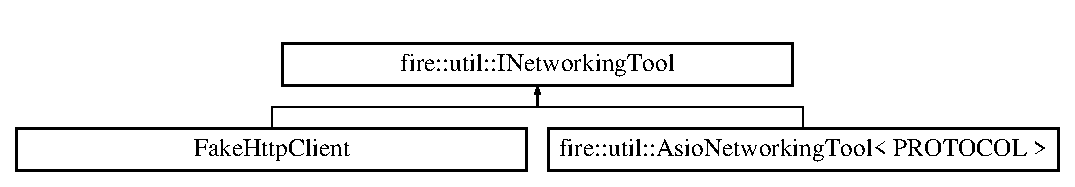
\includegraphics[height=2.000000cm]{a01976}
\end{center}
\end{figure}
\subsection*{Public Member Functions}
\begin{DoxyCompactItemize}
\item 
virtual std\+::string \hyperlink{a01976_a58e9426e58cbb9c3b975b9d3e6c1f78f}{get} (const std\+::string \&relative\+Path, const std\+::map$<$ std\+::string, std\+::string $>$ \&header=std\+::map$<$ std\+::string, std\+::string $>$())=0
\item 
virtual \hyperlink{a01972}{Post\+Response} \hyperlink{a01976_aa585d9b27c43f698203e6c6ec1ee05ce}{post} (const std\+::string \&relative\+Path, const std\+::string \&message, const std\+::map$<$ std\+::string, std\+::string $>$ \&header=std\+::map$<$ std\+::string, std\+::string $>$())=0
\item 
virtual \hyperlink{a01976_a2beca71d6ecb1688809f0e5e0548c17c}{$\sim$\+I\+Networking\+Tool} ()
\end{DoxyCompactItemize}
\subsection*{Protected Attributes}
\begin{DoxyCompactItemize}
\item 
std\+::string \hyperlink{a01976_ab7380b440faa49daffb65ca030380cde}{host\+Name}
\item 
int \hyperlink{a01976_ae640954c85632932a88037375a95abf4}{port}
\end{DoxyCompactItemize}


\subsection{Detailed Description}
The \hyperlink{a01976}{I\+Networking\+Tool} interface provides methods that enable typical H\+T\+TP G\+ET and P\+O\+ST behavior. 

\subsection{Constructor \& Destructor Documentation}
\mbox{\Hypertarget{a01976_a2beca71d6ecb1688809f0e5e0548c17c}\label{a01976_a2beca71d6ecb1688809f0e5e0548c17c}} 
\index{fire\+::util\+::\+I\+Networking\+Tool@{fire\+::util\+::\+I\+Networking\+Tool}!````~I\+Networking\+Tool@{$\sim$\+I\+Networking\+Tool}}
\index{````~I\+Networking\+Tool@{$\sim$\+I\+Networking\+Tool}!fire\+::util\+::\+I\+Networking\+Tool@{fire\+::util\+::\+I\+Networking\+Tool}}
\subsubsection{\texorpdfstring{$\sim$\+I\+Networking\+Tool()}{~INetworkingTool()}}
{\footnotesize\ttfamily virtual fire\+::util\+::\+I\+Networking\+Tool\+::$\sim$\+I\+Networking\+Tool (\begin{DoxyParamCaption}{ }\end{DoxyParamCaption})\hspace{0.3cm}{\ttfamily [inline]}, {\ttfamily [virtual]}}

virtual destructor 

\subsection{Member Function Documentation}
\mbox{\Hypertarget{a01976_a58e9426e58cbb9c3b975b9d3e6c1f78f}\label{a01976_a58e9426e58cbb9c3b975b9d3e6c1f78f}} 
\index{fire\+::util\+::\+I\+Networking\+Tool@{fire\+::util\+::\+I\+Networking\+Tool}!get@{get}}
\index{get@{get}!fire\+::util\+::\+I\+Networking\+Tool@{fire\+::util\+::\+I\+Networking\+Tool}}
\subsubsection{\texorpdfstring{get()}{get()}}
{\footnotesize\ttfamily virtual std\+::string fire\+::util\+::\+I\+Networking\+Tool\+::get (\begin{DoxyParamCaption}\item[{const std\+::string \&}]{relative\+Path,  }\item[{const std\+::map$<$ std\+::string, std\+::string $>$ \&}]{header = {\ttfamily std\+:\+:map$<$~std\+:\+:string,~std\+:\+:string~$>$()} }\end{DoxyParamCaption})\hspace{0.3cm}{\ttfamily [pure virtual]}}

Issue an H\+T\+TP G\+ET Command at the given relative path. Clients can provide a map of header key values to modify the G\+ET request.


\begin{DoxyParams}{Parameters}
{\em relative\+Path} & The path relative to the hostname/port provided to this Networking\+Tool \\
\hline
\end{DoxyParams}
\begin{DoxyReturn}{Returns}
The contents at the U\+RL or an error message if one took place. 
\end{DoxyReturn}


Implemented in \hyperlink{a01968_a40fed691e6b520a8e0f55734466896ca}{fire\+::util\+::\+Asio\+Networking\+Tool$<$ P\+R\+O\+T\+O\+C\+O\+L $>$}, and \hyperlink{a01224_a1bc1c2f1b3a0efb383aabb5a3a8080e6}{Fake\+Http\+Client}.

\mbox{\Hypertarget{a01976_aa585d9b27c43f698203e6c6ec1ee05ce}\label{a01976_aa585d9b27c43f698203e6c6ec1ee05ce}} 
\index{fire\+::util\+::\+I\+Networking\+Tool@{fire\+::util\+::\+I\+Networking\+Tool}!post@{post}}
\index{post@{post}!fire\+::util\+::\+I\+Networking\+Tool@{fire\+::util\+::\+I\+Networking\+Tool}}
\subsubsection{\texorpdfstring{post()}{post()}}
{\footnotesize\ttfamily virtual \hyperlink{a01972}{Post\+Response} fire\+::util\+::\+I\+Networking\+Tool\+::post (\begin{DoxyParamCaption}\item[{const std\+::string \&}]{relative\+Path,  }\item[{const std\+::string \&}]{message,  }\item[{const std\+::map$<$ std\+::string, std\+::string $>$ \&}]{header = {\ttfamily std\+:\+:map$<$~std\+:\+:string,~std\+:\+:string~$>$()} }\end{DoxyParamCaption})\hspace{0.3cm}{\ttfamily [pure virtual]}}

Issue an H\+T\+TP Post command at the given relative path with the provided message. Clients can provide a map of header key values to modify the P\+O\+ST request.


\begin{DoxyParams}{Parameters}
{\em relative\+Path} & The path relative to the hostname/port provided to this Networking\+Tool \\
\hline
{\em message} & The message to post \\
\hline
{\em header} & The map of additional H\+T\+TP P\+O\+ST header information \\
\hline
\end{DoxyParams}
\begin{DoxyReturn}{Returns}
post\+Response Struct containing state of post response 
\end{DoxyReturn}


Implemented in \hyperlink{a01968_a930b5535c0c68f54d01d4de36cc854a0}{fire\+::util\+::\+Asio\+Networking\+Tool$<$ P\+R\+O\+T\+O\+C\+O\+L $>$}, and \hyperlink{a01224_ae5364b5e675139717fca7b8add4226da}{Fake\+Http\+Client}.



\subsection{Member Data Documentation}
\mbox{\Hypertarget{a01976_ab7380b440faa49daffb65ca030380cde}\label{a01976_ab7380b440faa49daffb65ca030380cde}} 
\index{fire\+::util\+::\+I\+Networking\+Tool@{fire\+::util\+::\+I\+Networking\+Tool}!host\+Name@{host\+Name}}
\index{host\+Name@{host\+Name}!fire\+::util\+::\+I\+Networking\+Tool@{fire\+::util\+::\+I\+Networking\+Tool}}
\subsubsection{\texorpdfstring{host\+Name}{hostName}}
{\footnotesize\ttfamily std\+::string fire\+::util\+::\+I\+Networking\+Tool\+::host\+Name\hspace{0.3cm}{\ttfamily [protected]}}

The host name that this Networking\+Tool interacts with \mbox{\Hypertarget{a01976_ae640954c85632932a88037375a95abf4}\label{a01976_ae640954c85632932a88037375a95abf4}} 
\index{fire\+::util\+::\+I\+Networking\+Tool@{fire\+::util\+::\+I\+Networking\+Tool}!port@{port}}
\index{port@{port}!fire\+::util\+::\+I\+Networking\+Tool@{fire\+::util\+::\+I\+Networking\+Tool}}
\subsubsection{\texorpdfstring{port}{port}}
{\footnotesize\ttfamily int fire\+::util\+::\+I\+Networking\+Tool\+::port\hspace{0.3cm}{\ttfamily [protected]}}

The port on the host to establish connection with. 

The documentation for this class was generated from the following file\+:\begin{DoxyCompactItemize}
\item 
I\+Networking\+Tool.\+hpp\end{DoxyCompactItemize}

\hypertarget{a01744}{}\section{fire\+:\+:I\+N\+I\+Property\+Parser Class Reference}
\label{a01744}\index{fire\+::\+I\+N\+I\+Property\+Parser@{fire\+::\+I\+N\+I\+Property\+Parser}}


{\ttfamily \#include $<$I\+N\+I\+Property\+Parser.\+h$>$}

Inheritance diagram for fire\+:\+:I\+N\+I\+Property\+Parser\+:\begin{figure}[H]
\begin{center}
\leavevmode
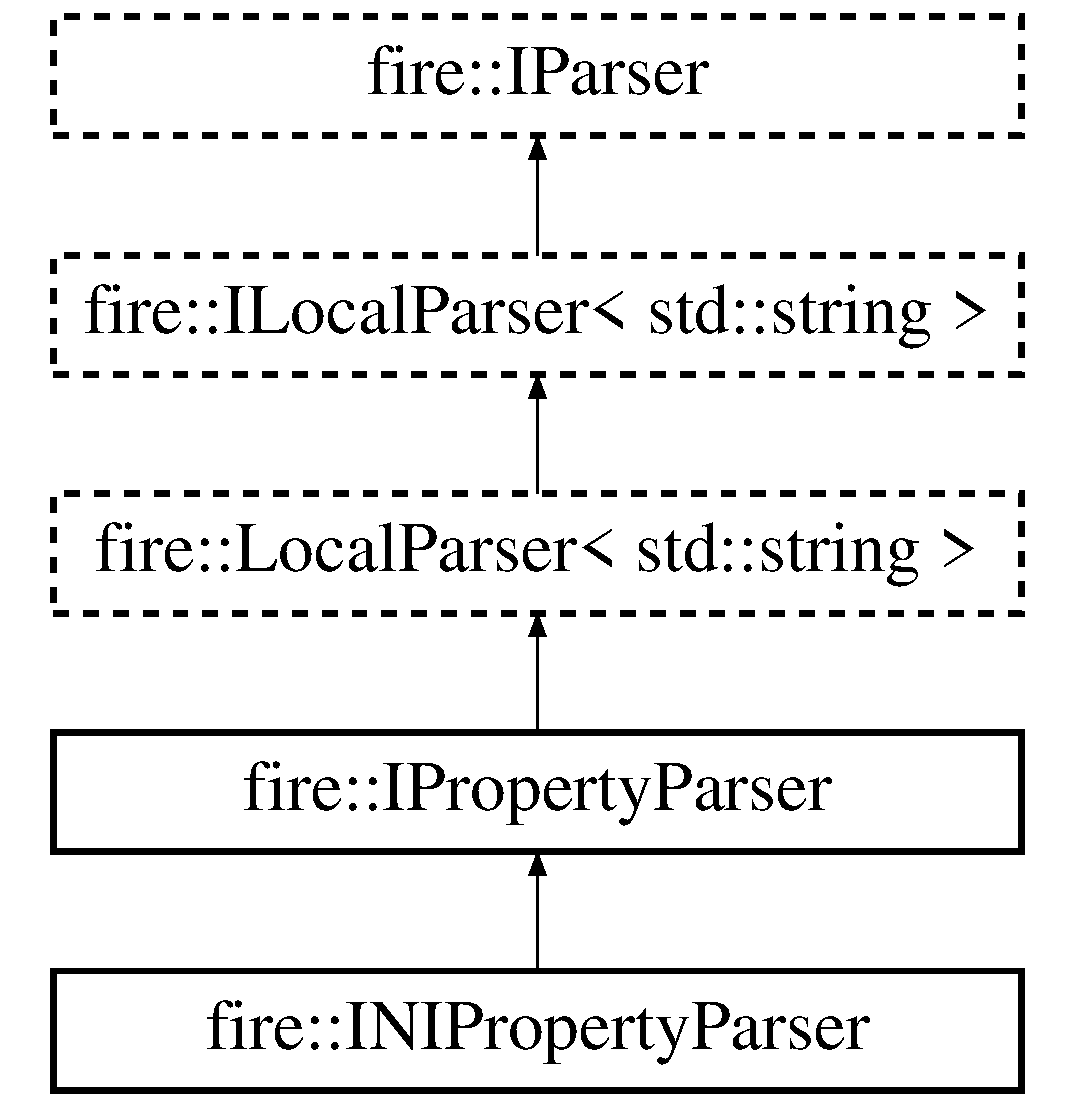
\includegraphics[height=5.000000cm]{a01744}
\end{center}
\end{figure}
\subsection*{Public Member Functions}
\begin{DoxyCompactItemize}
\item 
virtual void \hyperlink{a01744_a06793909bc707a69d0c5772b14bc946d}{set\+Source} (const std\+::string \&source)
\item 
virtual const std\+::string \& \hyperlink{a01744_ad02c9a530f20a706d7bb2554813e8d3a}{get\+Source} ()
\item 
virtual void \hyperlink{a01744_a31b6bad01e65ed4bb5f1ba297616c641}{parse} ()
\item 
virtual const std\+::vector$<$ std\+::string $>$ \& \hyperlink{a01744_aed0f1f47111794659564dcddb4d25bc6}{get\+Property\+Block\+Names} ()
\item 
virtual const std\+::map$<$ std\+::string, std\+::string $>$ \& \hyperlink{a01744_a3591312590a66659ebd377cdde9ab9ad}{get\+Property\+Block} (const std\+::string \&name)
\end{DoxyCompactItemize}
\subsection*{Additional Inherited Members}


\subsection{Detailed Description}
This class implements \hyperlink{a01752}{I\+Property\+Parser} to provide a local, file-\/based, serially executed I\+NI parser.

\hyperlink{a01740_a091d5cf56bf8f407854ef87f460b2958}{is\+File()} always returns true. \hyperlink{a01740_a770acae6e216de3a9c7140a12de25d58}{is\+Local()} always returns true. \hyperlink{a01740_ad46898c516adcce38acbb4800dc9777b}{is\+Parallel()} always returns false.

This implementation is backed by Simple\+I\+NI, one of Fire\textquotesingle{}s dependencies, so it supports whatever Simple\+I\+NI supports.

The source must be a file on the local filesystem. 

\subsection{Member Function Documentation}
\mbox{\Hypertarget{a01744_a3591312590a66659ebd377cdde9ab9ad}\label{a01744_a3591312590a66659ebd377cdde9ab9ad}} 
\index{fire\+::\+I\+N\+I\+Property\+Parser@{fire\+::\+I\+N\+I\+Property\+Parser}!get\+Property\+Block@{get\+Property\+Block}}
\index{get\+Property\+Block@{get\+Property\+Block}!fire\+::\+I\+N\+I\+Property\+Parser@{fire\+::\+I\+N\+I\+Property\+Parser}}
\subsubsection{\texorpdfstring{get\+Property\+Block()}{getPropertyBlock()}}
{\footnotesize\ttfamily virtual const std\+::map$<$std\+::string, std\+::string$>$\& fire\+::\+I\+N\+I\+Property\+Parser\+::get\+Property\+Block (\begin{DoxyParamCaption}\item[{const std\+::string \&}]{name }\end{DoxyParamCaption})\hspace{0.3cm}{\ttfamily [inline]}, {\ttfamily [virtual]}}

This operation returns the property block with the given name. 
\begin{DoxyParams}{Parameters}
{\em name} & the block name \\
\hline
\end{DoxyParams}
\begin{DoxyReturn}{Returns}
the property block with the given name 
\end{DoxyReturn}


Implements \hyperlink{a01752_a34201371cb36dd09e96a66242ececb86}{fire\+::\+I\+Property\+Parser}.

\mbox{\Hypertarget{a01744_aed0f1f47111794659564dcddb4d25bc6}\label{a01744_aed0f1f47111794659564dcddb4d25bc6}} 
\index{fire\+::\+I\+N\+I\+Property\+Parser@{fire\+::\+I\+N\+I\+Property\+Parser}!get\+Property\+Block\+Names@{get\+Property\+Block\+Names}}
\index{get\+Property\+Block\+Names@{get\+Property\+Block\+Names}!fire\+::\+I\+N\+I\+Property\+Parser@{fire\+::\+I\+N\+I\+Property\+Parser}}
\subsubsection{\texorpdfstring{get\+Property\+Block\+Names()}{getPropertyBlockNames()}}
{\footnotesize\ttfamily virtual const std\+::vector$<$std\+::string$>$\& fire\+::\+I\+N\+I\+Property\+Parser\+::get\+Property\+Block\+Names (\begin{DoxyParamCaption}{ }\end{DoxyParamCaption})\hspace{0.3cm}{\ttfamily [inline]}, {\ttfamily [virtual]}}

This operation returns the names of the property blocks parsed from the source. \begin{DoxyReturn}{Returns}
the block names 
\end{DoxyReturn}


Implements \hyperlink{a01752_a34602687f9d1affac7bd842102d4a6aa}{fire\+::\+I\+Property\+Parser}.

\mbox{\Hypertarget{a01744_ad02c9a530f20a706d7bb2554813e8d3a}\label{a01744_ad02c9a530f20a706d7bb2554813e8d3a}} 
\index{fire\+::\+I\+N\+I\+Property\+Parser@{fire\+::\+I\+N\+I\+Property\+Parser}!get\+Source@{get\+Source}}
\index{get\+Source@{get\+Source}!fire\+::\+I\+N\+I\+Property\+Parser@{fire\+::\+I\+N\+I\+Property\+Parser}}
\subsubsection{\texorpdfstring{get\+Source()}{getSource()}}
{\footnotesize\ttfamily virtual const std\+::string\& fire\+::\+I\+N\+I\+Property\+Parser\+::get\+Source (\begin{DoxyParamCaption}{ }\end{DoxyParamCaption})\hspace{0.3cm}{\ttfamily [inline]}, {\ttfamily [virtual]}}

This operation gets the data source for the parser. \begin{DoxyReturn}{Returns}
the name of the source 
\end{DoxyReturn}


Reimplemented from \hyperlink{a01756_aedb7fe10911182525a719963b9b56726}{fire\+::\+Local\+Parser$<$ std\+::string $>$}.

\mbox{\Hypertarget{a01744_a31b6bad01e65ed4bb5f1ba297616c641}\label{a01744_a31b6bad01e65ed4bb5f1ba297616c641}} 
\index{fire\+::\+I\+N\+I\+Property\+Parser@{fire\+::\+I\+N\+I\+Property\+Parser}!parse@{parse}}
\index{parse@{parse}!fire\+::\+I\+N\+I\+Property\+Parser@{fire\+::\+I\+N\+I\+Property\+Parser}}
\subsubsection{\texorpdfstring{parse()}{parse()}}
{\footnotesize\ttfamily virtual void fire\+::\+I\+N\+I\+Property\+Parser\+::parse (\begin{DoxyParamCaption}{ }\end{DoxyParamCaption})\hspace{0.3cm}{\ttfamily [inline]}, {\ttfamily [virtual]}}

This operation directs the parser to parse its source. 

Reimplemented from \hyperlink{a01756_abd8929aea06c2dda40256d2e58236650}{fire\+::\+Local\+Parser$<$ std\+::string $>$}.

\mbox{\Hypertarget{a01744_a06793909bc707a69d0c5772b14bc946d}\label{a01744_a06793909bc707a69d0c5772b14bc946d}} 
\index{fire\+::\+I\+N\+I\+Property\+Parser@{fire\+::\+I\+N\+I\+Property\+Parser}!set\+Source@{set\+Source}}
\index{set\+Source@{set\+Source}!fire\+::\+I\+N\+I\+Property\+Parser@{fire\+::\+I\+N\+I\+Property\+Parser}}
\subsubsection{\texorpdfstring{set\+Source()}{setSource()}}
{\footnotesize\ttfamily virtual void fire\+::\+I\+N\+I\+Property\+Parser\+::set\+Source (\begin{DoxyParamCaption}\item[{const std\+::string \&}]{source }\end{DoxyParamCaption})\hspace{0.3cm}{\ttfamily [inline]}, {\ttfamily [virtual]}}

This operation sets the data source for the parser. 
\begin{DoxyParams}{Parameters}
{\em source} & the name of the source that the parser should parse. \\
\hline
\end{DoxyParams}


Reimplemented from \hyperlink{a01756_afcaec6429fdd6e5d53642a32c001ff73}{fire\+::\+Local\+Parser$<$ std\+::string $>$}.



The documentation for this class was generated from the following file\+:\begin{DoxyCompactItemize}
\item 
I\+N\+I\+Property\+Parser.\+h\end{DoxyCompactItemize}

\hypertarget{a01836}{}\section{fire\+:\+:Initializer$<$ Fire\+Tensor, Scalar, N $>$ Struct Template Reference}
\label{a01836}\index{fire\+::\+Initializer$<$ Fire\+Tensor, Scalar, N $>$@{fire\+::\+Initializer$<$ Fire\+Tensor, Scalar, N $>$}}


{\ttfamily \#include $<$Tensor\+Utils.\+hpp$>$}

\subsection*{Public Types}
\begin{DoxyCompactItemize}
\item 
\mbox{\Hypertarget{a01836_aeb5626b5276d5c021ba8971b2d524c45}\label{a01836_aeb5626b5276d5c021ba8971b2d524c45}} 
typedef std\+::initializer\+\_\+list$<$ typename \hyperlink{a01836}{Initializer}$<$ \hyperlink{a01812}{Fire\+Tensor}, Scalar, N -\/ 1 $>$\+::Init\+List $>$ {\bfseries Init\+List}
\end{DoxyCompactItemize}


\subsection{Detailed Description}
\subsubsection*{template$<$typename Fire\+Tensor, typename Scalar, int N$>$\newline
struct fire\+::\+Initializer$<$ Fire\+Tensor, Scalar, N $>$}

The following three templates set up the recursion necessary to express nexted std\+::initializer\+\_\+lists. We use this to accept tensor values and set them on the internal \hyperlink{a01816}{Tensor\+Provider} tensor instance. 

The documentation for this struct was generated from the following file\+:\begin{DoxyCompactItemize}
\item 
Tensor\+Utils.\+hpp\end{DoxyCompactItemize}

\hypertarget{a01844}{}\section{fire\+:\+:Initializer$<$ Fire\+Tensor, Scalar, 0 $>$ Struct Template Reference}
\label{a01844}\index{fire\+::\+Initializer$<$ Fire\+Tensor, Scalar, 0 $>$@{fire\+::\+Initializer$<$ Fire\+Tensor, Scalar, 0 $>$}}
\subsection*{Public Types}
\begin{DoxyCompactItemize}
\item 
\mbox{\Hypertarget{a01844_aa3aa3da5b7d98e209a2c8f87d5a8371d}\label{a01844_aa3aa3da5b7d98e209a2c8f87d5a8371d}} 
typedef Scalar {\bfseries Init\+List}
\end{DoxyCompactItemize}


The documentation for this struct was generated from the following file\+:\begin{DoxyCompactItemize}
\item 
Tensor\+Utils.\+hpp\end{DoxyCompactItemize}

\hypertarget{a01840}{}\section{fire\+:\+:Initializer$<$ Fire\+Tensor, Scalar, 1 $>$ Struct Template Reference}
\label{a01840}\index{fire\+::\+Initializer$<$ Fire\+Tensor, Scalar, 1 $>$@{fire\+::\+Initializer$<$ Fire\+Tensor, Scalar, 1 $>$}}
\subsection*{Public Types}
\begin{DoxyCompactItemize}
\item 
\mbox{\Hypertarget{a01840_ab08b58675de0070598ae477a509856c8}\label{a01840_ab08b58675de0070598ae477a509856c8}} 
typedef std\+::initializer\+\_\+list$<$ Scalar $>$ {\bfseries Init\+List}
\end{DoxyCompactItemize}


The documentation for this struct was generated from the following file\+:\begin{DoxyCompactItemize}
\item 
Tensor\+Utils.\+hpp\end{DoxyCompactItemize}

\hypertarget{a02460}{}\section{xacc\+:\+:Instruction Class Reference}
\label{a02460}\index{xacc\+::\+Instruction@{xacc\+::\+Instruction}}


{\ttfamily \#include $<$Instruction.\+hpp$>$}

Inheritance diagram for xacc\+:\+:Instruction\+:\begin{figure}[H]
\begin{center}
\leavevmode
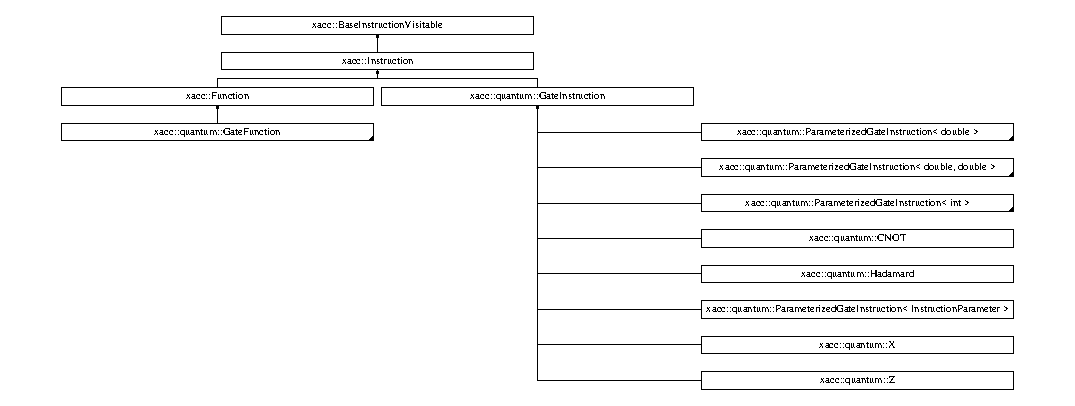
\includegraphics[height=5.008130cm]{a02460}
\end{center}
\end{figure}
\subsection*{Public Member Functions}
\begin{DoxyCompactItemize}
\item 
virtual const std\+::string \hyperlink{a02460_ac7ff23f693e2276edbf3fdac5452792c}{get\+Name} ()=0
\item 
virtual const std\+::string \hyperlink{a02460_ae94c2d089908294c1d410b14c96817ae}{to\+String} (const std\+::string \&buffer\+Var\+Name)=0
\item 
virtual const std\+::vector$<$ int $>$ \hyperlink{a02460_a819f32e94c3e1c9e69a0061aaf8d86dc}{bits} ()=0
\item 
virtual bool \hyperlink{a02460_a4383f1036d0fcfe890ab9c613dbd5f38}{is\+Composite} ()
\item 
virtual bool \hyperlink{a02460_ad02a1cf7220577124720b7a51424cea7}{is\+Enabled} ()
\item 
virtual void \hyperlink{a02460_a6e528da15e05a94cc1d7db268c483271}{disable} ()
\item 
virtual void \hyperlink{a02460_a0b4f2e5a591af28342a3c08e4305e24f}{enable} ()
\item 
virtual \hyperlink{a02460_ae22c935e8113bce63d1d0e214cda4d61}{$\sim$\+Instruction} ()
\end{DoxyCompactItemize}
\subsection*{Additional Inherited Members}


\subsection{Detailed Description}
The \hyperlink{a02460}{Instruction} interface is the base of all X\+A\+CC Intermediate Representation Instructions for post-\/\+Moore\textquotesingle{}s law accelerated computing. The \hyperlink{a02460}{Instruction}, at its core, provides an \hyperlink{a02460}{Instruction} name and a set of next-\/gen bits that the \hyperlink{a02460}{Instruction} operates on. Instructions can also be enabled or disabled. Instructions implement \hyperlink{a02476}{Base\+Instruction\+Visitable} to enable visitor pattern functionality across all \hyperlink{a02460}{Instruction} subclasses. 

\subsection{Constructor \& Destructor Documentation}
\mbox{\Hypertarget{a02460_ae22c935e8113bce63d1d0e214cda4d61}\label{a02460_ae22c935e8113bce63d1d0e214cda4d61}} 
\index{xacc\+::\+Instruction@{xacc\+::\+Instruction}!````~Instruction@{$\sim$\+Instruction}}
\index{````~Instruction@{$\sim$\+Instruction}!xacc\+::\+Instruction@{xacc\+::\+Instruction}}
\subsubsection{\texorpdfstring{$\sim$\+Instruction()}{~Instruction()}}
{\footnotesize\ttfamily virtual xacc\+::\+Instruction\+::$\sim$\+Instruction (\begin{DoxyParamCaption}{ }\end{DoxyParamCaption})\hspace{0.3cm}{\ttfamily [inline]}, {\ttfamily [virtual]}}

The destructor 

\subsection{Member Function Documentation}
\mbox{\Hypertarget{a02460_a819f32e94c3e1c9e69a0061aaf8d86dc}\label{a02460_a819f32e94c3e1c9e69a0061aaf8d86dc}} 
\index{xacc\+::\+Instruction@{xacc\+::\+Instruction}!bits@{bits}}
\index{bits@{bits}!xacc\+::\+Instruction@{xacc\+::\+Instruction}}
\subsubsection{\texorpdfstring{bits()}{bits()}}
{\footnotesize\ttfamily virtual const std\+::vector$<$int$>$ xacc\+::\+Instruction\+::bits (\begin{DoxyParamCaption}{ }\end{DoxyParamCaption})\hspace{0.3cm}{\ttfamily [pure virtual]}}

Return the indices of the bits that this \hyperlink{a02460}{Instruction} operates on.

\begin{DoxyReturn}{Returns}
bits The bits this \hyperlink{a02460}{Instruction} operates on. 
\end{DoxyReturn}


Implemented in \hyperlink{a01272_aba03de68b76a9e120705c3c389c714a1}{xacc\+::quantum\+::\+Gate\+Function}, and \hyperlink{a01276_ad32ad03dfc516e00093030e60178003d}{xacc\+::quantum\+::\+Gate\+Instruction}.

\mbox{\Hypertarget{a02460_a6e528da15e05a94cc1d7db268c483271}\label{a02460_a6e528da15e05a94cc1d7db268c483271}} 
\index{xacc\+::\+Instruction@{xacc\+::\+Instruction}!disable@{disable}}
\index{disable@{disable}!xacc\+::\+Instruction@{xacc\+::\+Instruction}}
\subsubsection{\texorpdfstring{disable()}{disable()}}
{\footnotesize\ttfamily virtual void xacc\+::\+Instruction\+::disable (\begin{DoxyParamCaption}{ }\end{DoxyParamCaption})\hspace{0.3cm}{\ttfamily [inline]}, {\ttfamily [virtual]}}

Disable this \hyperlink{a02460}{Instruction} 

Reimplemented in \hyperlink{a01276_a63ce138dd71fb43d303f5600fefb7215}{xacc\+::quantum\+::\+Gate\+Instruction}.

\mbox{\Hypertarget{a02460_a0b4f2e5a591af28342a3c08e4305e24f}\label{a02460_a0b4f2e5a591af28342a3c08e4305e24f}} 
\index{xacc\+::\+Instruction@{xacc\+::\+Instruction}!enable@{enable}}
\index{enable@{enable}!xacc\+::\+Instruction@{xacc\+::\+Instruction}}
\subsubsection{\texorpdfstring{enable()}{enable()}}
{\footnotesize\ttfamily virtual void xacc\+::\+Instruction\+::enable (\begin{DoxyParamCaption}{ }\end{DoxyParamCaption})\hspace{0.3cm}{\ttfamily [inline]}, {\ttfamily [virtual]}}

Enable this \hyperlink{a02460}{Instruction}. 

Reimplemented in \hyperlink{a01276_a7a80474b7fd465271b3313432db2e608}{xacc\+::quantum\+::\+Gate\+Instruction}.

\mbox{\Hypertarget{a02460_ac7ff23f693e2276edbf3fdac5452792c}\label{a02460_ac7ff23f693e2276edbf3fdac5452792c}} 
\index{xacc\+::\+Instruction@{xacc\+::\+Instruction}!get\+Name@{get\+Name}}
\index{get\+Name@{get\+Name}!xacc\+::\+Instruction@{xacc\+::\+Instruction}}
\subsubsection{\texorpdfstring{get\+Name()}{getName()}}
{\footnotesize\ttfamily virtual const std\+::string xacc\+::\+Instruction\+::get\+Name (\begin{DoxyParamCaption}{ }\end{DoxyParamCaption})\hspace{0.3cm}{\ttfamily [pure virtual]}}

Return the name of this \hyperlink{a02460}{Instruction}

\begin{DoxyReturn}{Returns}
name The name of this \hyperlink{a02460}{Instruction} 
\end{DoxyReturn}


Implemented in \hyperlink{a01272_af42efb6191267164717d53c469e15d3a}{xacc\+::quantum\+::\+Gate\+Function}, and \hyperlink{a01276_a0db03b9e46eeba1134f0ca2b83ccc842}{xacc\+::quantum\+::\+Gate\+Instruction}.

\mbox{\Hypertarget{a02460_a4383f1036d0fcfe890ab9c613dbd5f38}\label{a02460_a4383f1036d0fcfe890ab9c613dbd5f38}} 
\index{xacc\+::\+Instruction@{xacc\+::\+Instruction}!is\+Composite@{is\+Composite}}
\index{is\+Composite@{is\+Composite}!xacc\+::\+Instruction@{xacc\+::\+Instruction}}
\subsubsection{\texorpdfstring{is\+Composite()}{isComposite()}}
{\footnotesize\ttfamily virtual bool xacc\+::\+Instruction\+::is\+Composite (\begin{DoxyParamCaption}{ }\end{DoxyParamCaption})\hspace{0.3cm}{\ttfamily [inline]}, {\ttfamily [virtual]}}

Returns true if this \hyperlink{a02460}{Instruction} is composite, ie, contains other Instructions.

\begin{DoxyReturn}{Returns}
is\+Composite True if this is a composite \hyperlink{a02460}{Instruction} 
\end{DoxyReturn}


Reimplemented in \hyperlink{a02456_aa75500c657b5c3e0e36213e1506aad97}{xacc\+::\+Function}.

\mbox{\Hypertarget{a02460_ad02a1cf7220577124720b7a51424cea7}\label{a02460_ad02a1cf7220577124720b7a51424cea7}} 
\index{xacc\+::\+Instruction@{xacc\+::\+Instruction}!is\+Enabled@{is\+Enabled}}
\index{is\+Enabled@{is\+Enabled}!xacc\+::\+Instruction@{xacc\+::\+Instruction}}
\subsubsection{\texorpdfstring{is\+Enabled()}{isEnabled()}}
{\footnotesize\ttfamily virtual bool xacc\+::\+Instruction\+::is\+Enabled (\begin{DoxyParamCaption}{ }\end{DoxyParamCaption})\hspace{0.3cm}{\ttfamily [inline]}, {\ttfamily [virtual]}}

Returns true if this \hyperlink{a02460}{Instruction} is enabled

\begin{DoxyReturn}{Returns}
enabled True if this \hyperlink{a02460}{Instruction} is enabled. 
\end{DoxyReturn}


Reimplemented in \hyperlink{a01276_a0a821be322b0c848b01c55f91fc8f484}{xacc\+::quantum\+::\+Gate\+Instruction}.

\mbox{\Hypertarget{a02460_ae94c2d089908294c1d410b14c96817ae}\label{a02460_ae94c2d089908294c1d410b14c96817ae}} 
\index{xacc\+::\+Instruction@{xacc\+::\+Instruction}!to\+String@{to\+String}}
\index{to\+String@{to\+String}!xacc\+::\+Instruction@{xacc\+::\+Instruction}}
\subsubsection{\texorpdfstring{to\+String()}{toString()}}
{\footnotesize\ttfamily virtual const std\+::string xacc\+::\+Instruction\+::to\+String (\begin{DoxyParamCaption}\item[{const std\+::string \&}]{buffer\+Var\+Name }\end{DoxyParamCaption})\hspace{0.3cm}{\ttfamily [pure virtual]}}

Persist this \hyperlink{a02460}{Instruction} to an assembly-\/like string.


\begin{DoxyParams}{Parameters}
{\em buffer\+Var\+Name} & The name of the \hyperlink{a02444}{Accelerator\+Buffer} \\
\hline
\end{DoxyParams}
\begin{DoxyReturn}{Returns}
str The assembly-\/like string. 
\end{DoxyReturn}


Implemented in \hyperlink{a01280_aaccc4a20d58d2ac5c31abe7e325b8f77}{xacc\+::quantum\+::\+Parameterized\+Gate\+Instruction$<$ Instruction\+Parameter $>$}, \hyperlink{a01280_aaccc4a20d58d2ac5c31abe7e325b8f77}{xacc\+::quantum\+::\+Parameterized\+Gate\+Instruction$<$ double $>$}, \hyperlink{a01280_aaccc4a20d58d2ac5c31abe7e325b8f77}{xacc\+::quantum\+::\+Parameterized\+Gate\+Instruction$<$ int $>$}, \hyperlink{a01280_aaccc4a20d58d2ac5c31abe7e325b8f77}{xacc\+::quantum\+::\+Parameterized\+Gate\+Instruction$<$ double, double $>$}, \hyperlink{a01272_aa1950776ae84bad2d0795a0441f910e7}{xacc\+::quantum\+::\+Gate\+Function}, \hyperlink{a01276_a089a5da67ff40ac1a6f56e64589822d9}{xacc\+::quantum\+::\+Gate\+Instruction}, \hyperlink{a01312_a1c51a5d68294dcb2ba1a9fbea63a730f}{xacc\+::quantum\+::\+Measure}, and \hyperlink{a01304_aca7a5f849fece6fc28a904efee9a3370}{xacc\+::quantum\+::\+Conditional\+Function}.



The documentation for this class was generated from the following file\+:\begin{DoxyCompactItemize}
\item 
Instruction.\+hpp\end{DoxyCompactItemize}

\hypertarget{a02464}{}\section{xacc\+:\+:Instruction\+Iterator Class Reference}
\label{a02464}\index{xacc\+::\+Instruction\+Iterator@{xacc\+::\+Instruction\+Iterator}}


{\ttfamily \#include $<$Instruction\+Iterator.\+hpp$>$}

\subsection*{Public Member Functions}
\begin{DoxyCompactItemize}
\item 
\hyperlink{a02464_af61abf612341ab1454a1c43239b2da16}{Instruction\+Iterator} (std\+::shared\+\_\+ptr$<$ \hyperlink{a02460}{Instruction} $>$ r)
\item 
bool \hyperlink{a02464_a7fa6c8cff43e7b224211d4f7954a4152}{has\+Next} ()
\item 
std\+::shared\+\_\+ptr$<$ \hyperlink{a02460}{Instruction} $>$ \hyperlink{a02464_a0a2e2b1543650760a869460ebcd4382b}{next} ()
\end{DoxyCompactItemize}
\subsection*{Protected Attributes}
\begin{DoxyCompactItemize}
\item 
std\+::shared\+\_\+ptr$<$ \hyperlink{a02460}{Instruction} $>$ \hyperlink{a02464_a9d7aee1cb9058dd4a29c8fc71eeda57d}{root}
\item 
std\+::stack$<$ std\+::shared\+\_\+ptr$<$ \hyperlink{a02460}{Instruction} $>$ $>$ \hyperlink{a02464_a7af48509e563e8865131692c3b71edf0}{inst\+Stack}
\end{DoxyCompactItemize}


\subsection{Detailed Description}
The \hyperlink{a02464}{Instruction\+Iterator} provides a mechanism for a pre-\/order traversal of an \hyperlink{a02460}{Instruction} tree. 

\subsection{Constructor \& Destructor Documentation}
\mbox{\Hypertarget{a02464_af61abf612341ab1454a1c43239b2da16}\label{a02464_af61abf612341ab1454a1c43239b2da16}} 
\index{xacc\+::\+Instruction\+Iterator@{xacc\+::\+Instruction\+Iterator}!Instruction\+Iterator@{Instruction\+Iterator}}
\index{Instruction\+Iterator@{Instruction\+Iterator}!xacc\+::\+Instruction\+Iterator@{xacc\+::\+Instruction\+Iterator}}
\subsubsection{\texorpdfstring{Instruction\+Iterator()}{InstructionIterator()}}
{\footnotesize\ttfamily xacc\+::\+Instruction\+Iterator\+::\+Instruction\+Iterator (\begin{DoxyParamCaption}\item[{std\+::shared\+\_\+ptr$<$ \hyperlink{a02460}{Instruction} $>$}]{r }\end{DoxyParamCaption})\hspace{0.3cm}{\ttfamily [inline]}}

The constructor, takes the root of the tree as input.


\begin{DoxyParams}{Parameters}
{\em r} & \\
\hline
\end{DoxyParams}


\subsection{Member Function Documentation}
\mbox{\Hypertarget{a02464_a7fa6c8cff43e7b224211d4f7954a4152}\label{a02464_a7fa6c8cff43e7b224211d4f7954a4152}} 
\index{xacc\+::\+Instruction\+Iterator@{xacc\+::\+Instruction\+Iterator}!has\+Next@{has\+Next}}
\index{has\+Next@{has\+Next}!xacc\+::\+Instruction\+Iterator@{xacc\+::\+Instruction\+Iterator}}
\subsubsection{\texorpdfstring{has\+Next()}{hasNext()}}
{\footnotesize\ttfamily bool xacc\+::\+Instruction\+Iterator\+::has\+Next (\begin{DoxyParamCaption}{ }\end{DoxyParamCaption})\hspace{0.3cm}{\ttfamily [inline]}}

Return true if there are still instructions left to traverse. \begin{DoxyReturn}{Returns}

\end{DoxyReturn}
\mbox{\Hypertarget{a02464_a0a2e2b1543650760a869460ebcd4382b}\label{a02464_a0a2e2b1543650760a869460ebcd4382b}} 
\index{xacc\+::\+Instruction\+Iterator@{xacc\+::\+Instruction\+Iterator}!next@{next}}
\index{next@{next}!xacc\+::\+Instruction\+Iterator@{xacc\+::\+Instruction\+Iterator}}
\subsubsection{\texorpdfstring{next()}{next()}}
{\footnotesize\ttfamily std\+::shared\+\_\+ptr$<$\hyperlink{a02460}{Instruction}$>$ xacc\+::\+Instruction\+Iterator\+::next (\begin{DoxyParamCaption}{ }\end{DoxyParamCaption})\hspace{0.3cm}{\ttfamily [inline]}}

Return the next \hyperlink{a02460}{Instruction} in the tree. \begin{DoxyReturn}{Returns}

\end{DoxyReturn}


\subsection{Member Data Documentation}
\mbox{\Hypertarget{a02464_a7af48509e563e8865131692c3b71edf0}\label{a02464_a7af48509e563e8865131692c3b71edf0}} 
\index{xacc\+::\+Instruction\+Iterator@{xacc\+::\+Instruction\+Iterator}!inst\+Stack@{inst\+Stack}}
\index{inst\+Stack@{inst\+Stack}!xacc\+::\+Instruction\+Iterator@{xacc\+::\+Instruction\+Iterator}}
\subsubsection{\texorpdfstring{inst\+Stack}{instStack}}
{\footnotesize\ttfamily std\+::stack$<$std\+::shared\+\_\+ptr$<$\hyperlink{a02460}{Instruction}$>$ $>$ xacc\+::\+Instruction\+Iterator\+::inst\+Stack\hspace{0.3cm}{\ttfamily [protected]}}

A stack used to implement the tree traversal \mbox{\Hypertarget{a02464_a9d7aee1cb9058dd4a29c8fc71eeda57d}\label{a02464_a9d7aee1cb9058dd4a29c8fc71eeda57d}} 
\index{xacc\+::\+Instruction\+Iterator@{xacc\+::\+Instruction\+Iterator}!root@{root}}
\index{root@{root}!xacc\+::\+Instruction\+Iterator@{xacc\+::\+Instruction\+Iterator}}
\subsubsection{\texorpdfstring{root}{root}}
{\footnotesize\ttfamily std\+::shared\+\_\+ptr$<$\hyperlink{a02460}{Instruction}$>$ xacc\+::\+Instruction\+Iterator\+::root\hspace{0.3cm}{\ttfamily [protected]}}

The root of the tree, a function 

The documentation for this class was generated from the following file\+:\begin{DoxyCompactItemize}
\item 
Instruction\+Iterator.\+hpp\end{DoxyCompactItemize}

\hypertarget{a02472}{}\section{xacc\+:\+:Instruction\+Visitor$<$ T $>$ Class Template Reference}
\label{a02472}\index{xacc\+::\+Instruction\+Visitor$<$ T $>$@{xacc\+::\+Instruction\+Visitor$<$ T $>$}}


{\ttfamily \#include $<$Instruction\+Visitor.\+hpp$>$}

\subsection*{Public Member Functions}
\begin{DoxyCompactItemize}
\item 
virtual void \hyperlink{a02472_af0fead298f5bfbb8e6680433063e2c4b}{visit} (T \&)=0
\item 
virtual \hyperlink{a02472_adf624df25964d0be1a56af58639c9e1d}{$\sim$\+Instruction\+Visitor} ()
\end{DoxyCompactItemize}


\subsection{Detailed Description}
\subsubsection*{template$<$class T$>$\newline
class xacc\+::\+Instruction\+Visitor$<$ T $>$}

The \hyperlink{a02472}{Instruction\+Visitor} provides a visit method for the provided template parameter. 

\subsection{Constructor \& Destructor Documentation}
\mbox{\Hypertarget{a02472_adf624df25964d0be1a56af58639c9e1d}\label{a02472_adf624df25964d0be1a56af58639c9e1d}} 
\index{xacc\+::\+Instruction\+Visitor@{xacc\+::\+Instruction\+Visitor}!````~Instruction\+Visitor@{$\sim$\+Instruction\+Visitor}}
\index{````~Instruction\+Visitor@{$\sim$\+Instruction\+Visitor}!xacc\+::\+Instruction\+Visitor@{xacc\+::\+Instruction\+Visitor}}
\subsubsection{\texorpdfstring{$\sim$\+Instruction\+Visitor()}{~InstructionVisitor()}}
{\footnotesize\ttfamily template$<$class T$>$ \\
virtual \hyperlink{a02472}{xacc\+::\+Instruction\+Visitor}$<$ T $>$\+::$\sim$\hyperlink{a02472}{Instruction\+Visitor} (\begin{DoxyParamCaption}{ }\end{DoxyParamCaption})\hspace{0.3cm}{\ttfamily [inline]}, {\ttfamily [virtual]}}

The destructor 

\subsection{Member Function Documentation}
\mbox{\Hypertarget{a02472_af0fead298f5bfbb8e6680433063e2c4b}\label{a02472_af0fead298f5bfbb8e6680433063e2c4b}} 
\index{xacc\+::\+Instruction\+Visitor@{xacc\+::\+Instruction\+Visitor}!visit@{visit}}
\index{visit@{visit}!xacc\+::\+Instruction\+Visitor@{xacc\+::\+Instruction\+Visitor}}
\subsubsection{\texorpdfstring{visit()}{visit()}}
{\footnotesize\ttfamily template$<$class T$>$ \\
virtual void \hyperlink{a02472}{xacc\+::\+Instruction\+Visitor}$<$ T $>$\+::visit (\begin{DoxyParamCaption}\item[{T \&}]{ }\end{DoxyParamCaption})\hspace{0.3cm}{\ttfamily [pure virtual]}}

This method should be implemented by subclasses to perform Visitor-\/specific behavior on the given instance of the template parameter T. 

Implemented in \hyperlink{a01220_a144f1e4e6d24c450e0a941fa650c1f48}{Count\+Gate\+Visitor$<$ Gate\+Type $>$}.



The documentation for this class was generated from the following file\+:\begin{DoxyCompactItemize}
\item 
Instruction\+Visitor.\+hpp\end{DoxyCompactItemize}

\hypertarget{a02524}{}\section{xacc\+:\+:int\+\_\+$<$ size\+\_\+t $>$ Struct Template Reference}
\label{a02524}\index{xacc\+::int\+\_\+$<$ size\+\_\+t $>$@{xacc\+::int\+\_\+$<$ size\+\_\+t $>$}}


The documentation for this struct was generated from the following file\+:\begin{DoxyCompactItemize}
\item 
Graph.\+hpp\end{DoxyCompactItemize}

\hypertarget{a01748}{}\section{fire\+:\+:I\+Parser Class Reference}
\label{a01748}\index{fire\+::\+I\+Parser@{fire\+::\+I\+Parser}}


{\ttfamily \#include $<$I\+Parser.\+h$>$}

Inheritance diagram for fire\+:\+:I\+Parser\+:\begin{figure}[H]
\begin{center}
\leavevmode
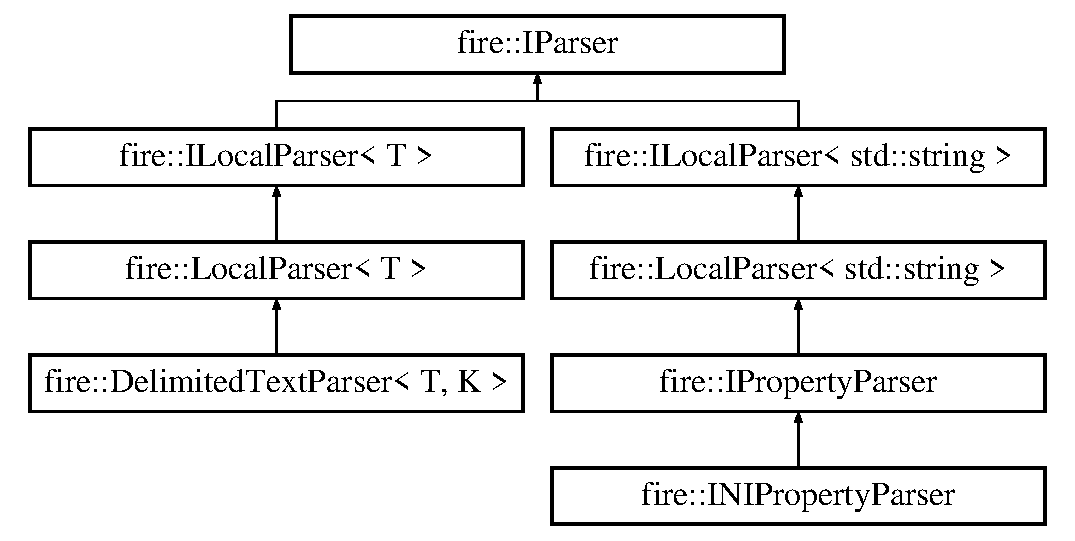
\includegraphics[height=5.000000cm]{a01748}
\end{center}
\end{figure}
\subsection*{Public Member Functions}
\begin{DoxyCompactItemize}
\item 
virtual void \hyperlink{a01748_a0dbeff2b9bd8dbfb2aad7a424eef87d1}{set\+Source} (const std\+::string \&source)=0
\item 
virtual const std\+::string \& \hyperlink{a01748_ab55d2644dfa6d950d1f874e1e02df095}{get\+Source} ()=0
\item 
virtual void \hyperlink{a01748_a7748a633910e9bfc27411d6bd840496b}{set\+Source} (const std\+::istream \&source)=0
\item 
virtual const std\+::istream \& \hyperlink{a01748_ac94c7a288bf669322b93ba171c43f90e}{get\+Source\+Stream} ()=0
\item 
virtual void \hyperlink{a01748_af36ac6eedd8c27d2f418869193d7d03c}{parse} ()=0
\item 
virtual bool \hyperlink{a01748_a616c42c85d781c916e97f0ad8f1e9010}{is\+File} ()=0
\item 
virtual bool \hyperlink{a01748_a97b9e58493b3cadbc63e670b0b0e759f}{is\+Local} ()=0
\item 
virtual bool \hyperlink{a01748_a83d2882a466d694fb0aea3d846bcbed4}{is\+Parallel} ()=0
\end{DoxyCompactItemize}


\subsection{Detailed Description}
This is the base interface for parsers in Fire and it defines the contract that can be expected of all parsers.

This source string is only a reference to the source or some sort of handle that points to it, such as a file or stream name. The exact type of the source -\/ file, stream, socket, etc. -\/ is determined by the implementing class. Check the documentation of implementing classes for the exact way the source string is used.

I\+Parsers should always be used by setting the source and then parsing the source\+:


\begin{DoxyCode}
IParser parser = ...;\textcolor{comment}{// somehow create your parser}
parser.setSource(sourceName);
parser.parser();
\end{DoxyCode}


Subclasses must always be sure that they implement \hyperlink{a01748_af36ac6eedd8c27d2f418869193d7d03c}{parse()} and \hyperlink{a01748_a0dbeff2b9bd8dbfb2aad7a424eef87d1}{set\+Source()}. 

\subsection{Member Function Documentation}
\mbox{\Hypertarget{a01748_ab55d2644dfa6d950d1f874e1e02df095}\label{a01748_ab55d2644dfa6d950d1f874e1e02df095}} 
\index{fire\+::\+I\+Parser@{fire\+::\+I\+Parser}!get\+Source@{get\+Source}}
\index{get\+Source@{get\+Source}!fire\+::\+I\+Parser@{fire\+::\+I\+Parser}}
\subsubsection{\texorpdfstring{get\+Source()}{getSource()}}
{\footnotesize\ttfamily virtual const std\+::string\& fire\+::\+I\+Parser\+::get\+Source (\begin{DoxyParamCaption}{ }\end{DoxyParamCaption})\hspace{0.3cm}{\ttfamily [pure virtual]}}

This operation gets the data source for the parser. \begin{DoxyReturn}{Returns}
the name of the source 
\end{DoxyReturn}


Implemented in \hyperlink{a01756_aedb7fe10911182525a719963b9b56726}{fire\+::\+Local\+Parser$<$ T $>$}, \hyperlink{a01756_aedb7fe10911182525a719963b9b56726}{fire\+::\+Local\+Parser$<$ std\+::string $>$}, and \hyperlink{a01744_ad02c9a530f20a706d7bb2554813e8d3a}{fire\+::\+I\+N\+I\+Property\+Parser}.

\mbox{\Hypertarget{a01748_ac94c7a288bf669322b93ba171c43f90e}\label{a01748_ac94c7a288bf669322b93ba171c43f90e}} 
\index{fire\+::\+I\+Parser@{fire\+::\+I\+Parser}!get\+Source\+Stream@{get\+Source\+Stream}}
\index{get\+Source\+Stream@{get\+Source\+Stream}!fire\+::\+I\+Parser@{fire\+::\+I\+Parser}}
\subsubsection{\texorpdfstring{get\+Source\+Stream()}{getSourceStream()}}
{\footnotesize\ttfamily virtual const std\+::istream\& fire\+::\+I\+Parser\+::get\+Source\+Stream (\begin{DoxyParamCaption}{ }\end{DoxyParamCaption})\hspace{0.3cm}{\ttfamily [pure virtual]}}

This operation gets the data source for the parser as a stream if and only if it was set as such. \begin{DoxyReturn}{Returns}
source the stream of delimited text data 
\end{DoxyReturn}


Implemented in \hyperlink{a01756_a9bf19a3cc9ae8ac0e6e7a0e7f6212cdc}{fire\+::\+Local\+Parser$<$ T $>$}, and \hyperlink{a01756_a9bf19a3cc9ae8ac0e6e7a0e7f6212cdc}{fire\+::\+Local\+Parser$<$ std\+::string $>$}.

\mbox{\Hypertarget{a01748_a616c42c85d781c916e97f0ad8f1e9010}\label{a01748_a616c42c85d781c916e97f0ad8f1e9010}} 
\index{fire\+::\+I\+Parser@{fire\+::\+I\+Parser}!is\+File@{is\+File}}
\index{is\+File@{is\+File}!fire\+::\+I\+Parser@{fire\+::\+I\+Parser}}
\subsubsection{\texorpdfstring{is\+File()}{isFile()}}
{\footnotesize\ttfamily virtual bool fire\+::\+I\+Parser\+::is\+File (\begin{DoxyParamCaption}{ }\end{DoxyParamCaption})\hspace{0.3cm}{\ttfamily [pure virtual]}}

This operation indicates whether or not the parser\textquotesingle{}s source is a file. \begin{DoxyReturn}{Returns}
true if this parser is working with a file, false otherwise. 
\end{DoxyReturn}


Implemented in \hyperlink{a01740_a091d5cf56bf8f407854ef87f460b2958}{fire\+::\+I\+Local\+Parser$<$ T $>$}, and \hyperlink{a01740_a091d5cf56bf8f407854ef87f460b2958}{fire\+::\+I\+Local\+Parser$<$ std\+::string $>$}.

\mbox{\Hypertarget{a01748_a97b9e58493b3cadbc63e670b0b0e759f}\label{a01748_a97b9e58493b3cadbc63e670b0b0e759f}} 
\index{fire\+::\+I\+Parser@{fire\+::\+I\+Parser}!is\+Local@{is\+Local}}
\index{is\+Local@{is\+Local}!fire\+::\+I\+Parser@{fire\+::\+I\+Parser}}
\subsubsection{\texorpdfstring{is\+Local()}{isLocal()}}
{\footnotesize\ttfamily virtual bool fire\+::\+I\+Parser\+::is\+Local (\begin{DoxyParamCaption}{ }\end{DoxyParamCaption})\hspace{0.3cm}{\ttfamily [pure virtual]}}

This operation indicates whether or not the parser is using a local source. \begin{DoxyReturn}{Returns}
true if this parser is working with a local source, false otherwise. 
\end{DoxyReturn}


Implemented in \hyperlink{a01740_a770acae6e216de3a9c7140a12de25d58}{fire\+::\+I\+Local\+Parser$<$ T $>$}, and \hyperlink{a01740_a770acae6e216de3a9c7140a12de25d58}{fire\+::\+I\+Local\+Parser$<$ std\+::string $>$}.

\mbox{\Hypertarget{a01748_a83d2882a466d694fb0aea3d846bcbed4}\label{a01748_a83d2882a466d694fb0aea3d846bcbed4}} 
\index{fire\+::\+I\+Parser@{fire\+::\+I\+Parser}!is\+Parallel@{is\+Parallel}}
\index{is\+Parallel@{is\+Parallel}!fire\+::\+I\+Parser@{fire\+::\+I\+Parser}}
\subsubsection{\texorpdfstring{is\+Parallel()}{isParallel()}}
{\footnotesize\ttfamily virtual bool fire\+::\+I\+Parser\+::is\+Parallel (\begin{DoxyParamCaption}{ }\end{DoxyParamCaption})\hspace{0.3cm}{\ttfamily [pure virtual]}}

This operation indicates whether or not the parser reads in parallel. \begin{DoxyReturn}{Returns}
true if this parser reads in parallel, false otherwise. 
\end{DoxyReturn}


Implemented in \hyperlink{a01740_ad46898c516adcce38acbb4800dc9777b}{fire\+::\+I\+Local\+Parser$<$ T $>$}, and \hyperlink{a01740_ad46898c516adcce38acbb4800dc9777b}{fire\+::\+I\+Local\+Parser$<$ std\+::string $>$}.

\mbox{\Hypertarget{a01748_af36ac6eedd8c27d2f418869193d7d03c}\label{a01748_af36ac6eedd8c27d2f418869193d7d03c}} 
\index{fire\+::\+I\+Parser@{fire\+::\+I\+Parser}!parse@{parse}}
\index{parse@{parse}!fire\+::\+I\+Parser@{fire\+::\+I\+Parser}}
\subsubsection{\texorpdfstring{parse()}{parse()}}
{\footnotesize\ttfamily virtual void fire\+::\+I\+Parser\+::parse (\begin{DoxyParamCaption}{ }\end{DoxyParamCaption})\hspace{0.3cm}{\ttfamily [pure virtual]}}

This operation directs the parser to parse its source. 

Implemented in \hyperlink{a01736_a773fa7ed28cb9d8c384ad94bd81fc93f}{fire\+::\+Delimited\+Text\+Parser$<$ T, K $>$}, \hyperlink{a01736_a686df5548771cae833d5e721442a821a}{fire\+::\+Delimited\+Text\+Parser$<$ T, K $>$}, \hyperlink{a01756_abd8929aea06c2dda40256d2e58236650}{fire\+::\+Local\+Parser$<$ T $>$}, \hyperlink{a01756_abd8929aea06c2dda40256d2e58236650}{fire\+::\+Local\+Parser$<$ std\+::string $>$}, \hyperlink{a01744_a31b6bad01e65ed4bb5f1ba297616c641}{fire\+::\+I\+N\+I\+Property\+Parser}, \hyperlink{a01756_ae904e264fe16708b3e434adea59e1b88}{fire\+::\+Local\+Parser$<$ T $>$}, \hyperlink{a01756_ae904e264fe16708b3e434adea59e1b88}{fire\+::\+Local\+Parser$<$ std\+::string $>$}, \hyperlink{a01756_a34fd9ffb0196c612c75b5288ed5e219b}{fire\+::\+Local\+Parser$<$ T $>$}, and \hyperlink{a01756_a34fd9ffb0196c612c75b5288ed5e219b}{fire\+::\+Local\+Parser$<$ std\+::string $>$}.

\mbox{\Hypertarget{a01748_a0dbeff2b9bd8dbfb2aad7a424eef87d1}\label{a01748_a0dbeff2b9bd8dbfb2aad7a424eef87d1}} 
\index{fire\+::\+I\+Parser@{fire\+::\+I\+Parser}!set\+Source@{set\+Source}}
\index{set\+Source@{set\+Source}!fire\+::\+I\+Parser@{fire\+::\+I\+Parser}}
\subsubsection{\texorpdfstring{set\+Source()}{setSource()}\hspace{0.1cm}{\footnotesize\ttfamily [1/2]}}
{\footnotesize\ttfamily virtual void fire\+::\+I\+Parser\+::set\+Source (\begin{DoxyParamCaption}\item[{const std\+::string \&}]{source }\end{DoxyParamCaption})\hspace{0.3cm}{\ttfamily [pure virtual]}}

This operation sets the data source for the parser. 
\begin{DoxyParams}{Parameters}
{\em source} & the name of the source that the parser should parse. \\
\hline
\end{DoxyParams}


Implemented in \hyperlink{a01756_afcaec6429fdd6e5d53642a32c001ff73}{fire\+::\+Local\+Parser$<$ T $>$}, \hyperlink{a01756_afcaec6429fdd6e5d53642a32c001ff73}{fire\+::\+Local\+Parser$<$ std\+::string $>$}, and \hyperlink{a01744_a06793909bc707a69d0c5772b14bc946d}{fire\+::\+I\+N\+I\+Property\+Parser}.

\mbox{\Hypertarget{a01748_a7748a633910e9bfc27411d6bd840496b}\label{a01748_a7748a633910e9bfc27411d6bd840496b}} 
\index{fire\+::\+I\+Parser@{fire\+::\+I\+Parser}!set\+Source@{set\+Source}}
\index{set\+Source@{set\+Source}!fire\+::\+I\+Parser@{fire\+::\+I\+Parser}}
\subsubsection{\texorpdfstring{set\+Source()}{setSource()}\hspace{0.1cm}{\footnotesize\ttfamily [2/2]}}
{\footnotesize\ttfamily virtual void fire\+::\+I\+Parser\+::set\+Source (\begin{DoxyParamCaption}\item[{const std\+::istream \&}]{source }\end{DoxyParamCaption})\hspace{0.3cm}{\ttfamily [pure virtual]}}

This operation sets the data source for the parser using a stream instead of a string. 
\begin{DoxyParams}{Parameters}
{\em source} & the stream of delimited text data \\
\hline
\end{DoxyParams}


Implemented in \hyperlink{a01756_aed4357541f2ff7d46f8846bd07bb3c42}{fire\+::\+Local\+Parser$<$ T $>$}, and \hyperlink{a01756_aed4357541f2ff7d46f8846bd07bb3c42}{fire\+::\+Local\+Parser$<$ std\+::string $>$}.



The documentation for this class was generated from the following file\+:\begin{DoxyCompactItemize}
\item 
I\+Parser.\+h\end{DoxyCompactItemize}

\hypertarget{a01752}{}\section{fire\+:\+:I\+Property\+Parser Class Reference}
\label{a01752}\index{fire\+::\+I\+Property\+Parser@{fire\+::\+I\+Property\+Parser}}


{\ttfamily \#include $<$I\+Property\+Parser.\+h$>$}

Inheritance diagram for fire\+:\+:I\+Property\+Parser\+:\begin{figure}[H]
\begin{center}
\leavevmode
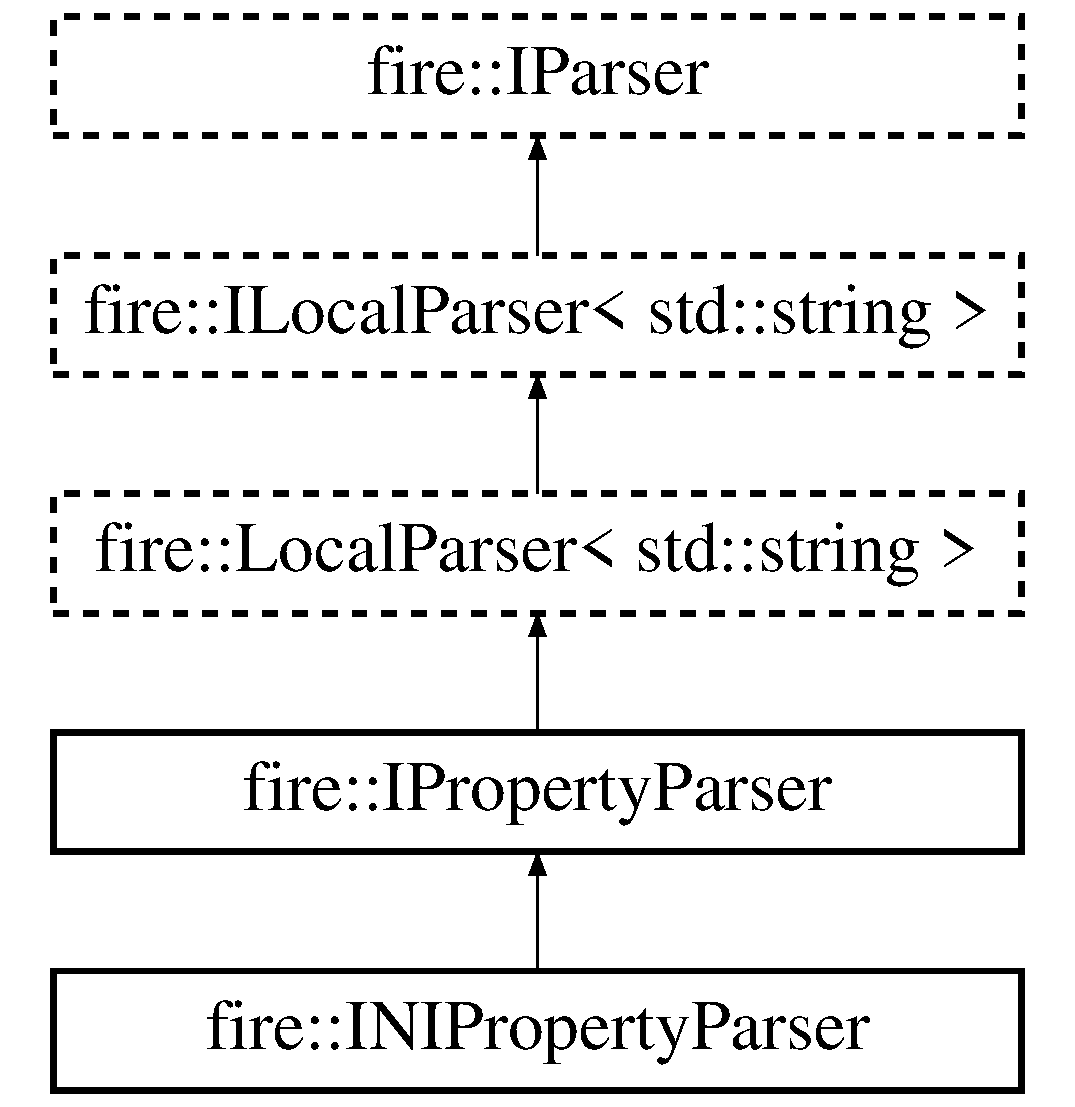
\includegraphics[height=5.000000cm]{a01752}
\end{center}
\end{figure}
\subsection*{Public Member Functions}
\begin{DoxyCompactItemize}
\item 
virtual const std\+::vector$<$ std\+::string $>$ \& \hyperlink{a01752_a34602687f9d1affac7bd842102d4a6aa}{get\+Property\+Block\+Names} ()=0
\item 
virtual const std\+::map$<$ std\+::string, std\+::string $>$ \& \hyperlink{a01752_a34201371cb36dd09e96a66242ececb86}{get\+Property\+Block} (const std\+::string \&name)=0
\end{DoxyCompactItemize}
\subsection*{Additional Inherited Members}


\subsection{Detailed Description}
This is an extension of the parser interface that focuses on parsing a set of properties. Properties are returned in blocks represented by maps.. 

\subsection{Member Function Documentation}
\mbox{\Hypertarget{a01752_a34201371cb36dd09e96a66242ececb86}\label{a01752_a34201371cb36dd09e96a66242ececb86}} 
\index{fire\+::\+I\+Property\+Parser@{fire\+::\+I\+Property\+Parser}!get\+Property\+Block@{get\+Property\+Block}}
\index{get\+Property\+Block@{get\+Property\+Block}!fire\+::\+I\+Property\+Parser@{fire\+::\+I\+Property\+Parser}}
\subsubsection{\texorpdfstring{get\+Property\+Block()}{getPropertyBlock()}}
{\footnotesize\ttfamily virtual const std\+::map$<$std\+::string, std\+::string$>$\& fire\+::\+I\+Property\+Parser\+::get\+Property\+Block (\begin{DoxyParamCaption}\item[{const std\+::string \&}]{name }\end{DoxyParamCaption})\hspace{0.3cm}{\ttfamily [pure virtual]}}

This operation returns the property block with the given name. 
\begin{DoxyParams}{Parameters}
{\em name} & the block name \\
\hline
\end{DoxyParams}
\begin{DoxyReturn}{Returns}
the property block with the given name 
\end{DoxyReturn}


Implemented in \hyperlink{a01744_a3591312590a66659ebd377cdde9ab9ad}{fire\+::\+I\+N\+I\+Property\+Parser}.

\mbox{\Hypertarget{a01752_a34602687f9d1affac7bd842102d4a6aa}\label{a01752_a34602687f9d1affac7bd842102d4a6aa}} 
\index{fire\+::\+I\+Property\+Parser@{fire\+::\+I\+Property\+Parser}!get\+Property\+Block\+Names@{get\+Property\+Block\+Names}}
\index{get\+Property\+Block\+Names@{get\+Property\+Block\+Names}!fire\+::\+I\+Property\+Parser@{fire\+::\+I\+Property\+Parser}}
\subsubsection{\texorpdfstring{get\+Property\+Block\+Names()}{getPropertyBlockNames()}}
{\footnotesize\ttfamily virtual const std\+::vector$<$std\+::string$>$\& fire\+::\+I\+Property\+Parser\+::get\+Property\+Block\+Names (\begin{DoxyParamCaption}{ }\end{DoxyParamCaption})\hspace{0.3cm}{\ttfamily [pure virtual]}}

This operation returns the names of the property blocks parsed from the source. \begin{DoxyReturn}{Returns}
the block names 
\end{DoxyReturn}


Implemented in \hyperlink{a01744_aed0f1f47111794659564dcddb4d25bc6}{fire\+::\+I\+N\+I\+Property\+Parser}.



The documentation for this class was generated from the following file\+:\begin{DoxyCompactItemize}
\item 
I\+Property\+Parser.\+h\end{DoxyCompactItemize}

\hypertarget{a02480}{}\section{xacc\+:\+:IR Class Reference}
\label{a02480}\index{xacc\+::\+IR@{xacc\+::\+IR}}


{\ttfamily \#include $<$I\+R.\+hpp$>$}

Inheritance diagram for xacc\+:\+:IR\+:\begin{figure}[H]
\begin{center}
\leavevmode
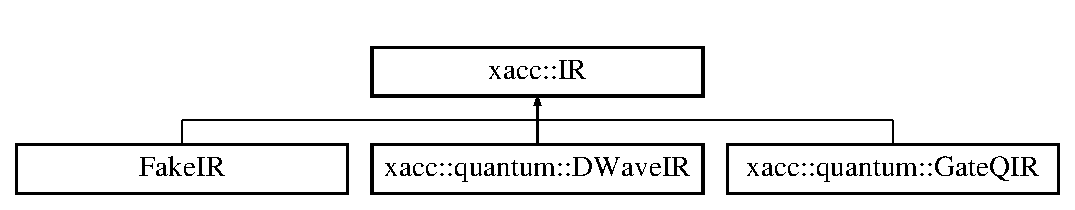
\includegraphics[height=2.000000cm]{a02480}
\end{center}
\end{figure}
\subsection*{Public Member Functions}
\begin{DoxyCompactItemize}
\item 
virtual std\+::string \hyperlink{a02480_a8356cdff1919b88eabeb84fd7450cdb6}{to\+Assembly\+String} (const std\+::string \&kernel\+Name, const std\+::string \&acc\+Buffer\+Var\+Name)=0
\item 
virtual void \hyperlink{a02480_a414b72224d88473ad6190bb88102a3ea}{persist} (std\+::ostream \&out\+Stream)=0
\item 
virtual void \hyperlink{a02480_a444c2e4dc0faac500fb70fa93997e9bc}{load} (std\+::istream \&in\+Stream)=0
\item 
virtual void \hyperlink{a02480_abbbf8e6993c518597de32cd05d49d737}{add\+Kernel} (std\+::shared\+\_\+ptr$<$ \hyperlink{a02456}{Function} $>$ kernel)=0
\item 
virtual std\+::shared\+\_\+ptr$<$ \hyperlink{a02456}{Function} $>$ \hyperlink{a02480_a6f49b4ba4b3a15142b04873284885f0d}{get\+Kernel} (const std\+::string \&name)=0
\item 
virtual \hyperlink{a02480_a09a76d71092254acae07e19fa2f34921}{$\sim$\+IR} ()
\end{DoxyCompactItemize}


\subsection{Detailed Description}
The \hyperlink{a02480}{IR} interface is the base interface for derived accelerator-\/specific intermediate representations. At this level, an intermediate representation can be persisted to an assembly-\/like string, can be read in from file, and can be persisted to file. Since all X\+A\+CC intermediate representations operate on an \hyperlink{a02432}{Accelerator} Buffer, the \hyperlink{a02480}{IR} interface also provides a setter for such a buffer. 

\subsection{Constructor \& Destructor Documentation}
\mbox{\Hypertarget{a02480_a09a76d71092254acae07e19fa2f34921}\label{a02480_a09a76d71092254acae07e19fa2f34921}} 
\index{xacc\+::\+IR@{xacc\+::\+IR}!````~IR@{$\sim$\+IR}}
\index{````~IR@{$\sim$\+IR}!xacc\+::\+IR@{xacc\+::\+IR}}
\subsubsection{\texorpdfstring{$\sim$\+I\+R()}{~IR()}}
{\footnotesize\ttfamily virtual xacc\+::\+I\+R\+::$\sim$\+IR (\begin{DoxyParamCaption}{ }\end{DoxyParamCaption})\hspace{0.3cm}{\ttfamily [inline]}, {\ttfamily [virtual]}}

The destructor 

\subsection{Member Function Documentation}
\mbox{\Hypertarget{a02480_abbbf8e6993c518597de32cd05d49d737}\label{a02480_abbbf8e6993c518597de32cd05d49d737}} 
\index{xacc\+::\+IR@{xacc\+::\+IR}!add\+Kernel@{add\+Kernel}}
\index{add\+Kernel@{add\+Kernel}!xacc\+::\+IR@{xacc\+::\+IR}}
\subsubsection{\texorpdfstring{add\+Kernel()}{addKernel()}}
{\footnotesize\ttfamily virtual void xacc\+::\+I\+R\+::add\+Kernel (\begin{DoxyParamCaption}\item[{std\+::shared\+\_\+ptr$<$ \hyperlink{a02456}{Function} $>$}]{kernel }\end{DoxyParamCaption})\hspace{0.3cm}{\ttfamily [pure virtual]}}

Add a new kernel to this \hyperlink{a02480}{IR} instance.


\begin{DoxyParams}{Parameters}
{\em kernel} & The \hyperlink{a02456}{Function} instance to add as a new kernel \\
\hline
\end{DoxyParams}


Implemented in \hyperlink{a01296_aa6ed2cf2cbcfec8105c327a4fa95346f}{xacc\+::quantum\+::\+Gate\+Q\+IR}, \hyperlink{a02492_a526ef10e1ee21f5552b1ca61872f541a}{Fake\+IR}, and \hyperlink{a01268_a7e1ddff2771233dc45f60a6b7e15ef63}{xacc\+::quantum\+::\+D\+Wave\+IR}.

\mbox{\Hypertarget{a02480_a6f49b4ba4b3a15142b04873284885f0d}\label{a02480_a6f49b4ba4b3a15142b04873284885f0d}} 
\index{xacc\+::\+IR@{xacc\+::\+IR}!get\+Kernel@{get\+Kernel}}
\index{get\+Kernel@{get\+Kernel}!xacc\+::\+IR@{xacc\+::\+IR}}
\subsubsection{\texorpdfstring{get\+Kernel()}{getKernel()}}
{\footnotesize\ttfamily virtual std\+::shared\+\_\+ptr$<$\hyperlink{a02456}{Function}$>$ xacc\+::\+I\+R\+::get\+Kernel (\begin{DoxyParamCaption}\item[{const std\+::string \&}]{name }\end{DoxyParamCaption})\hspace{0.3cm}{\ttfamily [pure virtual]}}

Return the kernel with the given name.


\begin{DoxyParams}{Parameters}
{\em name} & The name of the kernel to return. \\
\hline
\end{DoxyParams}
\begin{DoxyReturn}{Returns}
kernel The kernel with given name. 
\end{DoxyReturn}


Implemented in \hyperlink{a01296_a194758b6edcc3ae0c7fe8004f9bfe690}{xacc\+::quantum\+::\+Gate\+Q\+IR}, \hyperlink{a02492_a351b9a1f9fb748612f5a39007c421efc}{Fake\+IR}, and \hyperlink{a01268_ac4295dfef98c94d7154a4fd39a6e5d1c}{xacc\+::quantum\+::\+D\+Wave\+IR}.

\mbox{\Hypertarget{a02480_a444c2e4dc0faac500fb70fa93997e9bc}\label{a02480_a444c2e4dc0faac500fb70fa93997e9bc}} 
\index{xacc\+::\+IR@{xacc\+::\+IR}!load@{load}}
\index{load@{load}!xacc\+::\+IR@{xacc\+::\+IR}}
\subsubsection{\texorpdfstring{load()}{load()}}
{\footnotesize\ttfamily virtual void xacc\+::\+I\+R\+::load (\begin{DoxyParamCaption}\item[{std\+::istream \&}]{in\+Stream }\end{DoxyParamCaption})\hspace{0.3cm}{\ttfamily [pure virtual]}}

Create this \hyperlink{a02480}{IR} instance from the given input stream.


\begin{DoxyParams}{Parameters}
{\em in\+Stream} & The input stream to read from. \\
\hline
\end{DoxyParams}


Implemented in \hyperlink{a01296_a07f26eeb362ac480d20da6cdc8c8fb39}{xacc\+::quantum\+::\+Gate\+Q\+IR}, \hyperlink{a02492_ad079b5e83c97bc7fae776679e0f93a1e}{Fake\+IR}, and \hyperlink{a01268_a94d814172ec30c7ed32e6ab52bc2a41a}{xacc\+::quantum\+::\+D\+Wave\+IR}.

\mbox{\Hypertarget{a02480_a414b72224d88473ad6190bb88102a3ea}\label{a02480_a414b72224d88473ad6190bb88102a3ea}} 
\index{xacc\+::\+IR@{xacc\+::\+IR}!persist@{persist}}
\index{persist@{persist}!xacc\+::\+IR@{xacc\+::\+IR}}
\subsubsection{\texorpdfstring{persist()}{persist()}}
{\footnotesize\ttfamily virtual void xacc\+::\+I\+R\+::persist (\begin{DoxyParamCaption}\item[{std\+::ostream \&}]{out\+Stream }\end{DoxyParamCaption})\hspace{0.3cm}{\ttfamily [pure virtual]}}

Persist this \hyperlink{a02480}{IR} instance to the given output stream.


\begin{DoxyParams}{Parameters}
{\em out\+Stream} & The output stream to persist to. \\
\hline
\end{DoxyParams}


Implemented in \hyperlink{a01296_a40e1d07e4dfd3794ef53fca3cdbdca61}{xacc\+::quantum\+::\+Gate\+Q\+IR}, \hyperlink{a02492_a459bd7e4a007ab80678df279eb038b51}{Fake\+IR}, and \hyperlink{a01268_adac268c6fa2234902efeb9b3c07c0ac2}{xacc\+::quantum\+::\+D\+Wave\+IR}.

\mbox{\Hypertarget{a02480_a8356cdff1919b88eabeb84fd7450cdb6}\label{a02480_a8356cdff1919b88eabeb84fd7450cdb6}} 
\index{xacc\+::\+IR@{xacc\+::\+IR}!to\+Assembly\+String@{to\+Assembly\+String}}
\index{to\+Assembly\+String@{to\+Assembly\+String}!xacc\+::\+IR@{xacc\+::\+IR}}
\subsubsection{\texorpdfstring{to\+Assembly\+String()}{toAssemblyString()}}
{\footnotesize\ttfamily virtual std\+::string xacc\+::\+I\+R\+::to\+Assembly\+String (\begin{DoxyParamCaption}\item[{const std\+::string \&}]{kernel\+Name,  }\item[{const std\+::string \&}]{acc\+Buffer\+Var\+Name }\end{DoxyParamCaption})\hspace{0.3cm}{\ttfamily [pure virtual]}}

Return a assembly-\/like string representation of this intermediate representation


\begin{DoxyParams}{Parameters}
{\em kernel\+Name} & The name of hte kernel to persist to string \\
\hline
{\em acc\+Buffer\+Var\+Name} & The name of the \hyperlink{a02444}{Accelerator\+Buffer} \\
\hline
\end{DoxyParams}
\begin{DoxyReturn}{Returns}

\end{DoxyReturn}


Implemented in \hyperlink{a01296_a7153f7e9f516d43af3d5d4f95d60bd86}{xacc\+::quantum\+::\+Gate\+Q\+IR}, \hyperlink{a02492_ac8b4fa63654de7830e2a6110559ffd87}{Fake\+IR}, and \hyperlink{a01268_ac19ad098d5bbfe769809c10e26ebebc6}{xacc\+::quantum\+::\+D\+Wave\+IR}.



The documentation for this class was generated from the following file\+:\begin{DoxyCompactItemize}
\item 
I\+R.\+hpp\end{DoxyCompactItemize}

\hypertarget{a02484}{}\section{xacc\+:\+:I\+R\+Transformation Class Reference}
\label{a02484}\index{xacc\+::\+I\+R\+Transformation@{xacc\+::\+I\+R\+Transformation}}
\subsection*{Public Member Functions}
\begin{DoxyCompactItemize}
\item 
\mbox{\Hypertarget{a02484_accc69cba97f39aa3e51f81fec3ccf258}\label{a02484_accc69cba97f39aa3e51f81fec3ccf258}} 
virtual void {\bfseries transform} (\hyperlink{a02480}{IR} \&ir)=0
\end{DoxyCompactItemize}


The documentation for this class was generated from the following file\+:\begin{DoxyCompactItemize}
\item 
I\+R\+Transformation.\+hpp\end{DoxyCompactItemize}

\hypertarget{a01448}{}\section{boost\+:\+:dll\+:\+:experimental\+:\+:detail\+:\+:is\+\_\+function\+\_\+seq$<$ T $>$ Struct Template Reference}
\label{a01448}\index{boost\+::dll\+::experimental\+::detail\+::is\+\_\+function\+\_\+seq$<$ T $>$@{boost\+::dll\+::experimental\+::detail\+::is\+\_\+function\+\_\+seq$<$ T $>$}}


The documentation for this struct was generated from the following file\+:\begin{DoxyCompactItemize}
\item 
import\+\_\+mangled\+\_\+helpers.\+hpp\end{DoxyCompactItemize}

\hypertarget{a01456}{}\section{boost\+:\+:dll\+:\+:experimental\+:\+:detail\+:\+:is\+\_\+function\+\_\+seq$<$ sequence$<$ Class $>$ $>$ Struct Template Reference}
\label{a01456}\index{boost\+::dll\+::experimental\+::detail\+::is\+\_\+function\+\_\+seq$<$ sequence$<$ Class $>$ $>$@{boost\+::dll\+::experimental\+::detail\+::is\+\_\+function\+\_\+seq$<$ sequence$<$ Class $>$ $>$}}
Inheritance diagram for boost\+:\+:dll\+:\+:experimental\+:\+:detail\+:\+:is\+\_\+function\+\_\+seq$<$ sequence$<$ Class $>$ $>$\+:\begin{figure}[H]
\begin{center}
\leavevmode
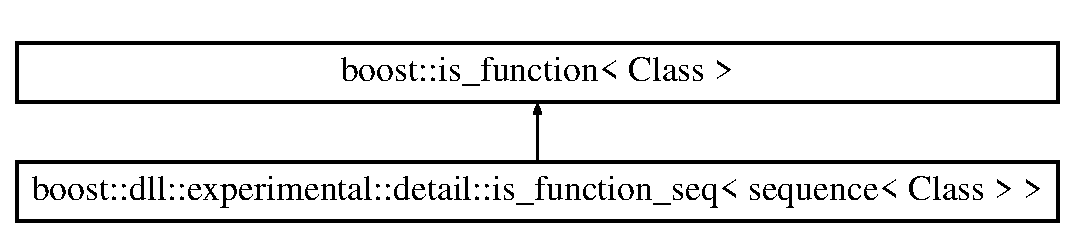
\includegraphics[height=2.000000cm]{a01456}
\end{center}
\end{figure}


The documentation for this struct was generated from the following file\+:\begin{DoxyCompactItemize}
\item 
import\+\_\+mangled\+\_\+helpers.\+hpp\end{DoxyCompactItemize}

\hypertarget{a01452}{}\section{boost\+:\+:dll\+:\+:experimental\+:\+:detail\+:\+:is\+\_\+function\+\_\+seq$<$ sequence$<$ Class, Args... $>$ $>$ Struct Template Reference}
\label{a01452}\index{boost\+::dll\+::experimental\+::detail\+::is\+\_\+function\+\_\+seq$<$ sequence$<$ Class, Args... $>$ $>$@{boost\+::dll\+::experimental\+::detail\+::is\+\_\+function\+\_\+seq$<$ sequence$<$ Class, Args... $>$ $>$}}
Inheritance diagram for boost\+:\+:dll\+:\+:experimental\+:\+:detail\+:\+:is\+\_\+function\+\_\+seq$<$ sequence$<$ Class, Args... $>$ $>$\+:\begin{figure}[H]
\begin{center}
\leavevmode
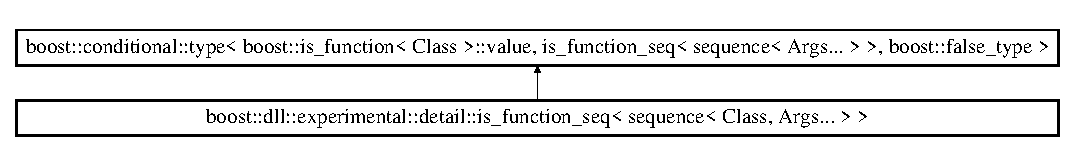
\includegraphics[height=1.600000cm]{a01452}
\end{center}
\end{figure}


The documentation for this struct was generated from the following file\+:\begin{DoxyCompactItemize}
\item 
import\+\_\+mangled\+\_\+helpers.\+hpp\end{DoxyCompactItemize}

\hypertarget{a01460}{}\section{boost\+:\+:dll\+:\+:experimental\+:\+:detail\+:\+:is\+\_\+function\+\_\+seq$<$ sequence$<$$>$ $>$ Struct Template Reference}
\label{a01460}\index{boost\+::dll\+::experimental\+::detail\+::is\+\_\+function\+\_\+seq$<$ sequence$<$$>$ $>$@{boost\+::dll\+::experimental\+::detail\+::is\+\_\+function\+\_\+seq$<$ sequence$<$$>$ $>$}}
Inheritance diagram for boost\+:\+:dll\+:\+:experimental\+:\+:detail\+:\+:is\+\_\+function\+\_\+seq$<$ sequence$<$$>$ $>$\+:\begin{figure}[H]
\begin{center}
\leavevmode
\includegraphics[height=2.000000cm]{a01460}
\end{center}
\end{figure}


The documentation for this struct was generated from the following file\+:\begin{DoxyCompactItemize}
\item 
import\+\_\+mangled\+\_\+helpers.\+hpp\end{DoxyCompactItemize}

\hypertarget{a01520}{}\section{boost\+:\+:dll\+:\+:experimental\+:\+:detail\+:\+:is\+\_\+mem\+\_\+fn\+\_\+seq$<$ T $>$ Struct Template Reference}
\label{a01520}\index{boost\+::dll\+::experimental\+::detail\+::is\+\_\+mem\+\_\+fn\+\_\+seq$<$ T $>$@{boost\+::dll\+::experimental\+::detail\+::is\+\_\+mem\+\_\+fn\+\_\+seq$<$ T $>$}}
Inheritance diagram for boost\+:\+:dll\+:\+:experimental\+:\+:detail\+:\+:is\+\_\+mem\+\_\+fn\+\_\+seq$<$ T $>$\+:\begin{figure}[H]
\begin{center}
\leavevmode
\includegraphics[height=2.000000cm]{a01520}
\end{center}
\end{figure}


The documentation for this struct was generated from the following file\+:\begin{DoxyCompactItemize}
\item 
import\+\_\+mangled\+\_\+helpers.\+hpp\end{DoxyCompactItemize}

\hypertarget{a01528}{}\section{boost\+:\+:dll\+:\+:experimental\+:\+:detail\+:\+:is\+\_\+mem\+\_\+fn\+\_\+seq$<$ sequence$<$ T, Func, Args... $>$ $>$ Struct Template Reference}
\label{a01528}\index{boost\+::dll\+::experimental\+::detail\+::is\+\_\+mem\+\_\+fn\+\_\+seq$<$ sequence$<$ T, Func, Args... $>$ $>$@{boost\+::dll\+::experimental\+::detail\+::is\+\_\+mem\+\_\+fn\+\_\+seq$<$ sequence$<$ T, Func, Args... $>$ $>$}}
Inheritance diagram for boost\+:\+:dll\+:\+:experimental\+:\+:detail\+:\+:is\+\_\+mem\+\_\+fn\+\_\+seq$<$ sequence$<$ T, Func, Args... $>$ $>$\+:\begin{figure}[H]
\begin{center}
\leavevmode
\includegraphics[height=1.294798cm]{a01528}
\end{center}
\end{figure}


The documentation for this struct was generated from the following file\+:\begin{DoxyCompactItemize}
\item 
import\+\_\+mangled\+\_\+helpers.\+hpp\end{DoxyCompactItemize}

\hypertarget{a01524}{}\section{boost\+:\+:dll\+:\+:experimental\+:\+:detail\+:\+:is\+\_\+mem\+\_\+fn\+\_\+seq$<$ sequence$<$ T, U $>$ $>$ Struct Template Reference}
\label{a01524}\index{boost\+::dll\+::experimental\+::detail\+::is\+\_\+mem\+\_\+fn\+\_\+seq$<$ sequence$<$ T, U $>$ $>$@{boost\+::dll\+::experimental\+::detail\+::is\+\_\+mem\+\_\+fn\+\_\+seq$<$ sequence$<$ T, U $>$ $>$}}
Inheritance diagram for boost\+:\+:dll\+:\+:experimental\+:\+:detail\+:\+:is\+\_\+mem\+\_\+fn\+\_\+seq$<$ sequence$<$ T, U $>$ $>$\+:\begin{figure}[H]
\begin{center}
\leavevmode
\includegraphics[height=1.566434cm]{a01524}
\end{center}
\end{figure}


The documentation for this struct was generated from the following file\+:\begin{DoxyCompactItemize}
\item 
import\+\_\+mangled\+\_\+helpers.\+hpp\end{DoxyCompactItemize}

\hypertarget{a01508}{}\section{boost\+:\+:dll\+:\+:experimental\+:\+:detail\+:\+:is\+\_\+mem\+\_\+fn\+\_\+seq\+\_\+impl$<$ T, U, Args $>$ Struct Template Reference}
\label{a01508}\index{boost\+::dll\+::experimental\+::detail\+::is\+\_\+mem\+\_\+fn\+\_\+seq\+\_\+impl$<$ T, U, Args $>$@{boost\+::dll\+::experimental\+::detail\+::is\+\_\+mem\+\_\+fn\+\_\+seq\+\_\+impl$<$ T, U, Args $>$}}
\subsection*{Public Types}
\begin{DoxyCompactItemize}
\item 
\mbox{\Hypertarget{a01508_a5b0ef01b378457cb1ffabfae4a1ed68f}\label{a01508_a5b0ef01b378457cb1ffabfae4a1ed68f}} 
typedef boost\+::conditional$<$ boost\+::is\+\_\+function$<$ U $>$\+::value$\vert$$\vert$\hyperlink{a01444}{boost\+::dll\+::experimental\+::detail\+::unqalified\+\_\+is\+\_\+same}$<$ T, U $>$\+::value, typename \hyperlink{a01508}{is\+\_\+mem\+\_\+fn\+\_\+seq\+\_\+impl}$<$ T, Args... $>$\+::type, boost\+::false\+\_\+type $>$\+::type {\bfseries type}
\end{DoxyCompactItemize}


The documentation for this struct was generated from the following file\+:\begin{DoxyCompactItemize}
\item 
import\+\_\+mangled\+\_\+helpers.\+hpp\end{DoxyCompactItemize}

\hypertarget{a01512}{}\section{boost\+:\+:dll\+:\+:experimental\+:\+:detail\+:\+:is\+\_\+mem\+\_\+fn\+\_\+seq\+\_\+impl$<$ T, U $>$ Struct Template Reference}
\label{a01512}\index{boost\+::dll\+::experimental\+::detail\+::is\+\_\+mem\+\_\+fn\+\_\+seq\+\_\+impl$<$ T, U $>$@{boost\+::dll\+::experimental\+::detail\+::is\+\_\+mem\+\_\+fn\+\_\+seq\+\_\+impl$<$ T, U $>$}}
\subsection*{Public Types}
\begin{DoxyCompactItemize}
\item 
\mbox{\Hypertarget{a01512_aec1a5860cdcd1498eaeb3ce7ee7f5373}\label{a01512_aec1a5860cdcd1498eaeb3ce7ee7f5373}} 
typedef boost\+::conditional$<$ boost\+::is\+\_\+function$<$ U $>$\+::value \&\&boost\+::is\+\_\+object$<$ T $>$\+::value, boost\+::true\+\_\+type, boost\+::false\+\_\+type $>$\+::type {\bfseries type}
\end{DoxyCompactItemize}


The documentation for this struct was generated from the following file\+:\begin{DoxyCompactItemize}
\item 
import\+\_\+mangled\+\_\+helpers.\+hpp\end{DoxyCompactItemize}

\hypertarget{a01516}{}\section{boost\+:\+:dll\+:\+:experimental\+:\+:detail\+:\+:is\+\_\+mem\+\_\+fn\+\_\+seq\+\_\+impl$<$ T, U, Last $>$ Struct Template Reference}
\label{a01516}\index{boost\+::dll\+::experimental\+::detail\+::is\+\_\+mem\+\_\+fn\+\_\+seq\+\_\+impl$<$ T, U, Last $>$@{boost\+::dll\+::experimental\+::detail\+::is\+\_\+mem\+\_\+fn\+\_\+seq\+\_\+impl$<$ T, U, Last $>$}}
\subsection*{Public Types}
\begin{DoxyCompactItemize}
\item 
\mbox{\Hypertarget{a01516_a4689022563a599f3389c7defc6210274}\label{a01516_a4689022563a599f3389c7defc6210274}} 
typedef boost\+::conditional$<$(boost\+::is\+\_\+function$<$ U $>$\+::value$\vert$$\vert$\hyperlink{a01444}{boost\+::dll\+::experimental\+::detail\+::unqalified\+\_\+is\+\_\+same}$<$ T, U $>$\+::value) \&\&boost\+::is\+\_\+function$<$ Last $>$\+::value, boost\+::true\+\_\+type, boost\+::false\+\_\+type $>$\+::type {\bfseries type}
\end{DoxyCompactItemize}


The documentation for this struct was generated from the following file\+:\begin{DoxyCompactItemize}
\item 
import\+\_\+mangled\+\_\+helpers.\+hpp\end{DoxyCompactItemize}

\hypertarget{a02508}{}\section{xacc\+:\+:is\+\_\+valid\+\_\+vertex$<$ T, typename $>$ Struct Template Reference}
\label{a02508}\index{xacc\+::is\+\_\+valid\+\_\+vertex$<$ T, typename $>$@{xacc\+::is\+\_\+valid\+\_\+vertex$<$ T, typename $>$}}


{\ttfamily \#include $<$Graph.\+hpp$>$}

Inheritance diagram for xacc\+:\+:is\+\_\+valid\+\_\+vertex$<$ T, typename $>$\+:\begin{figure}[H]
\begin{center}
\leavevmode
\includegraphics[height=2.000000cm]{a02508}
\end{center}
\end{figure}


\subsection{Detailed Description}
\subsubsection*{template$<$typename T, typename = void$>$\newline
struct xacc\+::is\+\_\+valid\+\_\+vertex$<$ T, typename $>$}

Utility structs to help determine if we have been given valid Vertices. 

The documentation for this struct was generated from the following file\+:\begin{DoxyCompactItemize}
\item 
Graph.\+hpp\end{DoxyCompactItemize}

\hypertarget{a02512}{}\section{xacc\+:\+:is\+\_\+valid\+\_\+vertex$<$ T, decltype(std\+:\+:declval$<$ T $>$().properties, void())$>$ Struct Template Reference}
\label{a02512}\index{xacc\+::is\+\_\+valid\+\_\+vertex$<$ T, decltype(std\+::declval$<$ T $>$().\+properties, void())$>$@{xacc\+::is\+\_\+valid\+\_\+vertex$<$ T, decltype(std\+::declval$<$ T $>$().\+properties, void())$>$}}
Inheritance diagram for xacc\+:\+:is\+\_\+valid\+\_\+vertex$<$ T, decltype(std\+:\+:declval$<$ T $>$().properties, void())$>$\+:\begin{figure}[H]
\begin{center}
\leavevmode
\includegraphics[height=2.000000cm]{a02512}
\end{center}
\end{figure}


The documentation for this struct was generated from the following file\+:\begin{DoxyCompactItemize}
\item 
Graph.\+hpp\end{DoxyCompactItemize}

\hypertarget{a01680}{}\section{boost\+:\+:dll\+:\+:experimental\+:\+:detail\+:\+:is\+\_\+variable$<$ Seq $>$ Struct Template Reference}
\label{a01680}\index{boost\+::dll\+::experimental\+::detail\+::is\+\_\+variable$<$ Seq $>$@{boost\+::dll\+::experimental\+::detail\+::is\+\_\+variable$<$ Seq $>$}}
Inheritance diagram for boost\+:\+:dll\+:\+:experimental\+:\+:detail\+:\+:is\+\_\+variable$<$ Seq $>$\+:\begin{figure}[H]
\begin{center}
\leavevmode
\includegraphics[height=2.000000cm]{a01680}
\end{center}
\end{figure}


The documentation for this struct was generated from the following file\+:\begin{DoxyCompactItemize}
\item 
import\+\_\+mangled.\+hpp\end{DoxyCompactItemize}

\hypertarget{a01684}{}\section{boost\+:\+:dll\+:\+:experimental\+:\+:detail\+:\+:is\+\_\+variable$<$ sequence$<$ T $>$ $>$ Struct Template Reference}
\label{a01684}\index{boost\+::dll\+::experimental\+::detail\+::is\+\_\+variable$<$ sequence$<$ T $>$ $>$@{boost\+::dll\+::experimental\+::detail\+::is\+\_\+variable$<$ sequence$<$ T $>$ $>$}}
Inheritance diagram for boost\+:\+:dll\+:\+:experimental\+:\+:detail\+:\+:is\+\_\+variable$<$ sequence$<$ T $>$ $>$\+:\begin{figure}[H]
\begin{center}
\leavevmode
\includegraphics[height=2.000000cm]{a01684}
\end{center}
\end{figure}


The documentation for this struct was generated from the following file\+:\begin{DoxyCompactItemize}
\item 
import\+\_\+mangled.\+hpp\end{DoxyCompactItemize}

\hypertarget{a02364}{}\section{internal\+:\+:I\+Schema\+State\+Factory$<$ Schema\+Type $>$ Class Template Reference}
\label{a02364}\index{internal\+::\+I\+Schema\+State\+Factory$<$ Schema\+Type $>$@{internal\+::\+I\+Schema\+State\+Factory$<$ Schema\+Type $>$}}
\subsection*{Public Member Functions}
\begin{DoxyCompactItemize}
\item 
\mbox{\Hypertarget{a02364_ae8c98fcff6a057b4fcd9018fc14551a8}\label{a02364_ae8c98fcff6a057b4fcd9018fc14551a8}} 
virtual \hyperlink{a02360}{I\+Schema\+Validator} $\ast$ {\bfseries Create\+Schema\+Validator} (const Schema\+Type \&)=0
\item 
\mbox{\Hypertarget{a02364_a112cbf154077050bc30ffe670032442c}\label{a02364_a112cbf154077050bc30ffe670032442c}} 
virtual void {\bfseries Destroy\+Schema\+Validator} (\hyperlink{a02360}{I\+Schema\+Validator} $\ast$validator)=0
\item 
\mbox{\Hypertarget{a02364_a4ac37b9d3e9526004c82692473f978f4}\label{a02364_a4ac37b9d3e9526004c82692473f978f4}} 
virtual void $\ast$ {\bfseries Create\+Hasher} ()=0
\item 
\mbox{\Hypertarget{a02364_addfcf00963cc777edf642b204f07c8d6}\label{a02364_addfcf00963cc777edf642b204f07c8d6}} 
virtual uint64\+\_\+t {\bfseries Get\+Hash\+Code} (void $\ast$hasher)=0
\item 
\mbox{\Hypertarget{a02364_a70b8d88180d2e6993105b17f19101635}\label{a02364_a70b8d88180d2e6993105b17f19101635}} 
virtual void {\bfseries Destrory\+Hasher} (void $\ast$hasher)=0
\item 
\mbox{\Hypertarget{a02364_ada92ebf8e9ef994f7e20a0f7f9750519}\label{a02364_ada92ebf8e9ef994f7e20a0f7f9750519}} 
virtual void $\ast$ {\bfseries Malloc\+State} (size\+\_\+t size)=0
\item 
\mbox{\Hypertarget{a02364_a27bd2138940cac3c330dd8399c49b22b}\label{a02364_a27bd2138940cac3c330dd8399c49b22b}} 
virtual void {\bfseries Free\+State} (void $\ast$p)=0
\end{DoxyCompactItemize}


The documentation for this class was generated from the following file\+:\begin{DoxyCompactItemize}
\item 
schema.\+h\end{DoxyCompactItemize}

\hypertarget{a02360}{}\section{internal\+:\+:I\+Schema\+Validator Class Reference}
\label{a02360}\index{internal\+::\+I\+Schema\+Validator@{internal\+::\+I\+Schema\+Validator}}
Inheritance diagram for internal\+:\+:I\+Schema\+Validator\+:\begin{figure}[H]
\begin{center}
\leavevmode
\includegraphics[height=2.000000cm]{a02360}
\end{center}
\end{figure}
\subsection*{Public Member Functions}
\begin{DoxyCompactItemize}
\item 
\mbox{\Hypertarget{a02360_a94f61f24b1447497279ef12ee0127285}\label{a02360_a94f61f24b1447497279ef12ee0127285}} 
virtual bool {\bfseries Is\+Valid} () const =0
\end{DoxyCompactItemize}


The documentation for this class was generated from the following file\+:\begin{DoxyCompactItemize}
\item 
schema.\+h\end{DoxyCompactItemize}

\hypertarget{a02020}{}\section{internal\+:\+:Is\+Generic\+Value$<$ T $>$ Struct Template Reference}
\label{a02020}\index{internal\+::\+Is\+Generic\+Value$<$ T $>$@{internal\+::\+Is\+Generic\+Value$<$ T $>$}}
Inheritance diagram for internal\+:\+:Is\+Generic\+Value$<$ T $>$\+:\begin{figure}[H]
\begin{center}
\leavevmode
\includegraphics[height=2.000000cm]{a02020}
\end{center}
\end{figure}


The documentation for this struct was generated from the following file\+:\begin{DoxyCompactItemize}
\item 
\hyperlink{a00476}{document.\+h}\end{DoxyCompactItemize}

\hypertarget{a02012}{}\section{internal\+:\+:Is\+Generic\+Value\+Impl$<$ T, Encoding, Allocator $>$ Struct Template Reference}
\label{a02012}\index{internal\+::\+Is\+Generic\+Value\+Impl$<$ T, Encoding, Allocator $>$@{internal\+::\+Is\+Generic\+Value\+Impl$<$ T, Encoding, Allocator $>$}}
Inheritance diagram for internal\+:\+:Is\+Generic\+Value\+Impl$<$ T, Encoding, Allocator $>$\+:\begin{figure}[H]
\begin{center}
\leavevmode
\includegraphics[height=2.000000cm]{a02012}
\end{center}
\end{figure}


The documentation for this struct was generated from the following file\+:\begin{DoxyCompactItemize}
\item 
\hyperlink{a00476}{document.\+h}\end{DoxyCompactItemize}

\hypertarget{a02016}{}\section{internal\+:\+:Is\+Generic\+Value\+Impl$<$ T, typename Void$<$ typename T\+:\+:Encoding\+Type $>$\+:\+:Type, typename Void$<$ typename T\+:\+:Allocator\+Type $>$\+:\+:Type $>$ Struct Template Reference}
\label{a02016}\index{internal\+::\+Is\+Generic\+Value\+Impl$<$ T, typename Void$<$ typename T\+::\+Encoding\+Type $>$\+::\+Type, typename Void$<$ typename T\+::\+Allocator\+Type $>$\+::\+Type $>$@{internal\+::\+Is\+Generic\+Value\+Impl$<$ T, typename Void$<$ typename T\+::\+Encoding\+Type $>$\+::\+Type, typename Void$<$ typename T\+::\+Allocator\+Type $>$\+::\+Type $>$}}
Inheritance diagram for internal\+:\+:Is\+Generic\+Value\+Impl$<$ T, typename Void$<$ typename T\+:\+:Encoding\+Type $>$\+:\+:Type, typename Void$<$ typename T\+:\+:Allocator\+Type $>$\+:\+:Type $>$\+:\begin{figure}[H]
\begin{center}
\leavevmode
\includegraphics[height=1.372549cm]{a02016}
\end{center}
\end{figure}


The documentation for this struct was generated from the following file\+:\begin{DoxyCompactItemize}
\item 
\hyperlink{a00476}{document.\+h}\end{DoxyCompactItemize}

\hypertarget{a01728}{}\section{fire\+:\+:I\+Stepper Class Reference}
\label{a01728}\index{fire\+::\+I\+Stepper@{fire\+::\+I\+Stepper}}


{\ttfamily \#include $<$I\+Stepper.\+h$>$}

Inheritance diagram for fire\+:\+:I\+Stepper\+:\begin{figure}[H]
\begin{center}
\leavevmode
\includegraphics[height=2.000000cm]{a01728}
\end{center}
\end{figure}
\subsection*{Public Member Functions}
\begin{DoxyCompactItemize}
\item 
virtual double \hyperlink{a01728_a7f709d1462a2a3b8bd8214cc681ca26e}{get\+Step} ()=0
\item 
virtual double \hyperlink{a01728_a43027c0c268afcd59db8815c2e2c41ea}{get\+Step\+Size\+At\+Stage} (int i)=0
\item 
virtual void \hyperlink{a01728_a44dfccb90ee5ef6e080b54113c215458}{update\+Step} ()=0
\item 
virtual void \hyperlink{a01728_a3a5099cd0f3c874e56c33cb8f13b8f3b}{set\+Initial\+Step} (double initial\+Step)=0
\item 
virtual double \hyperlink{a01728_a49df3a2ac05cebaf2baf387b66d19272}{get\+Initial\+Step} ()=0
\item 
virtual void \hyperlink{a01728_add76974a7b6fbbc93916270a376c461e}{set\+Final\+Step} (double final\+Step)=0
\item 
virtual double \hyperlink{a01728_ab234d9f032e02668aededf1c22e8c0a9}{get\+Final\+Step} ()=0
\item 
virtual void \hyperlink{a01728_a69c262f248511efcd271be1724a41ad9}{set\+Initial\+Stepsize} (double step\+Size)=0
\item 
virtual double \hyperlink{a01728_afb777e62386b25e5a38d59af54972690}{get\+Initial\+Stepsize} ()=0
\item 
virtual \hyperlink{a01728_ac8ec460d35512e2e039396d5192eb57e}{$\sim$\+I\+Stepper} ()
\end{DoxyCompactItemize}


\subsection{Detailed Description}
This is an interface for managing discrete steps as required by Initial Value Problem Integrators. \hyperlink{a01728}{I\+Stepper} implementations track both the step and the stepsize. In the case of time-\/dependent initial value problems, implementations would be called \char`\"{}time steppers\char`\"{} and would be responsible for computing both the present time (the step) and the step between the present size and the next (the step size). In purely spatial or otherwise on-\/temporal problems, the step represents the current value of the independent variable and the step size represents the distance between the present and next steps.

This interface is designed for single-\/ and multi-\/stage solvers, such as Runge-\/\+Kutta solvers. 

\subsection{Constructor \& Destructor Documentation}
\mbox{\Hypertarget{a01728_ac8ec460d35512e2e039396d5192eb57e}\label{a01728_ac8ec460d35512e2e039396d5192eb57e}} 
\index{fire\+::\+I\+Stepper@{fire\+::\+I\+Stepper}!````~I\+Stepper@{$\sim$\+I\+Stepper}}
\index{````~I\+Stepper@{$\sim$\+I\+Stepper}!fire\+::\+I\+Stepper@{fire\+::\+I\+Stepper}}
\subsubsection{\texorpdfstring{$\sim$\+I\+Stepper()}{~IStepper()}}
{\footnotesize\ttfamily virtual fire\+::\+I\+Stepper\+::$\sim$\+I\+Stepper (\begin{DoxyParamCaption}{ }\end{DoxyParamCaption})\hspace{0.3cm}{\ttfamily [inline]}, {\ttfamily [virtual]}}

Virtual Destructor 

\subsection{Member Function Documentation}
\mbox{\Hypertarget{a01728_ab234d9f032e02668aededf1c22e8c0a9}\label{a01728_ab234d9f032e02668aededf1c22e8c0a9}} 
\index{fire\+::\+I\+Stepper@{fire\+::\+I\+Stepper}!get\+Final\+Step@{get\+Final\+Step}}
\index{get\+Final\+Step@{get\+Final\+Step}!fire\+::\+I\+Stepper@{fire\+::\+I\+Stepper}}
\subsubsection{\texorpdfstring{get\+Final\+Step()}{getFinalStep()}}
{\footnotesize\ttfamily virtual double fire\+::\+I\+Stepper\+::get\+Final\+Step (\begin{DoxyParamCaption}{ }\end{DoxyParamCaption})\hspace{0.3cm}{\ttfamily [pure virtual]}}

This operation returns the final step for the stepper. \begin{DoxyReturn}{Returns}
the final step 
\end{DoxyReturn}


Implemented in \hyperlink{a01732_ae6f257aca7b3bb62a851169a01bcaacf}{fire\+::\+Profile\+Stepper}.

\mbox{\Hypertarget{a01728_a49df3a2ac05cebaf2baf387b66d19272}\label{a01728_a49df3a2ac05cebaf2baf387b66d19272}} 
\index{fire\+::\+I\+Stepper@{fire\+::\+I\+Stepper}!get\+Initial\+Step@{get\+Initial\+Step}}
\index{get\+Initial\+Step@{get\+Initial\+Step}!fire\+::\+I\+Stepper@{fire\+::\+I\+Stepper}}
\subsubsection{\texorpdfstring{get\+Initial\+Step()}{getInitialStep()}}
{\footnotesize\ttfamily virtual double fire\+::\+I\+Stepper\+::get\+Initial\+Step (\begin{DoxyParamCaption}{ }\end{DoxyParamCaption})\hspace{0.3cm}{\ttfamily [pure virtual]}}

This operation returns the initial step for the stepper. \begin{DoxyReturn}{Returns}
the initial step 
\end{DoxyReturn}


Implemented in \hyperlink{a01732_af24660fa4bd027f877d5c1bdeb286cf5}{fire\+::\+Profile\+Stepper}.

\mbox{\Hypertarget{a01728_afb777e62386b25e5a38d59af54972690}\label{a01728_afb777e62386b25e5a38d59af54972690}} 
\index{fire\+::\+I\+Stepper@{fire\+::\+I\+Stepper}!get\+Initial\+Stepsize@{get\+Initial\+Stepsize}}
\index{get\+Initial\+Stepsize@{get\+Initial\+Stepsize}!fire\+::\+I\+Stepper@{fire\+::\+I\+Stepper}}
\subsubsection{\texorpdfstring{get\+Initial\+Stepsize()}{getInitialStepsize()}}
{\footnotesize\ttfamily virtual double fire\+::\+I\+Stepper\+::get\+Initial\+Stepsize (\begin{DoxyParamCaption}{ }\end{DoxyParamCaption})\hspace{0.3cm}{\ttfamily [pure virtual]}}

This operation gets the initial step size for the stepper \begin{DoxyReturn}{Returns}
the initial step size 
\end{DoxyReturn}


Implemented in \hyperlink{a01732_a86e7035366907a08a36722655746271e}{fire\+::\+Profile\+Stepper}.

\mbox{\Hypertarget{a01728_a7f709d1462a2a3b8bd8214cc681ca26e}\label{a01728_a7f709d1462a2a3b8bd8214cc681ca26e}} 
\index{fire\+::\+I\+Stepper@{fire\+::\+I\+Stepper}!get\+Step@{get\+Step}}
\index{get\+Step@{get\+Step}!fire\+::\+I\+Stepper@{fire\+::\+I\+Stepper}}
\subsubsection{\texorpdfstring{get\+Step()}{getStep()}}
{\footnotesize\ttfamily virtual double fire\+::\+I\+Stepper\+::get\+Step (\begin{DoxyParamCaption}{ }\end{DoxyParamCaption})\hspace{0.3cm}{\ttfamily [pure virtual]}}

This operation returns the step value for the current step. \begin{DoxyReturn}{Returns}
the step value 
\end{DoxyReturn}


Implemented in \hyperlink{a01732_a9096ad65a3fcf63678b600cbe0c33961}{fire\+::\+Profile\+Stepper}.

\mbox{\Hypertarget{a01728_a43027c0c268afcd59db8815c2e2c41ea}\label{a01728_a43027c0c268afcd59db8815c2e2c41ea}} 
\index{fire\+::\+I\+Stepper@{fire\+::\+I\+Stepper}!get\+Step\+Size\+At\+Stage@{get\+Step\+Size\+At\+Stage}}
\index{get\+Step\+Size\+At\+Stage@{get\+Step\+Size\+At\+Stage}!fire\+::\+I\+Stepper@{fire\+::\+I\+Stepper}}
\subsubsection{\texorpdfstring{get\+Step\+Size\+At\+Stage()}{getStepSizeAtStage()}}
{\footnotesize\ttfamily virtual double fire\+::\+I\+Stepper\+::get\+Step\+Size\+At\+Stage (\begin{DoxyParamCaption}\item[{int}]{i }\end{DoxyParamCaption})\hspace{0.3cm}{\ttfamily [pure virtual]}}

This operation returns the step size for the given stage. 
\begin{DoxyParams}{Parameters}
{\em the} & stage of the solver for which the stepsize should be computed \\
\hline
\end{DoxyParams}
\begin{DoxyReturn}{Returns}
the step size 
\end{DoxyReturn}


Implemented in \hyperlink{a01732_adaa1a23c068977ecc6809dd8eecab49d}{fire\+::\+Profile\+Stepper}.

\mbox{\Hypertarget{a01728_add76974a7b6fbbc93916270a376c461e}\label{a01728_add76974a7b6fbbc93916270a376c461e}} 
\index{fire\+::\+I\+Stepper@{fire\+::\+I\+Stepper}!set\+Final\+Step@{set\+Final\+Step}}
\index{set\+Final\+Step@{set\+Final\+Step}!fire\+::\+I\+Stepper@{fire\+::\+I\+Stepper}}
\subsubsection{\texorpdfstring{set\+Final\+Step()}{setFinalStep()}}
{\footnotesize\ttfamily virtual void fire\+::\+I\+Stepper\+::set\+Final\+Step (\begin{DoxyParamCaption}\item[{double}]{final\+Step }\end{DoxyParamCaption})\hspace{0.3cm}{\ttfamily [pure virtual]}}

This operation sets the final step for the stepper. 
\begin{DoxyParams}{Parameters}
{\em final\+Step} & the final step \\
\hline
\end{DoxyParams}


Implemented in \hyperlink{a01732_af8203296b4f3bef53bafab7cb654cc97}{fire\+::\+Profile\+Stepper}.

\mbox{\Hypertarget{a01728_a3a5099cd0f3c874e56c33cb8f13b8f3b}\label{a01728_a3a5099cd0f3c874e56c33cb8f13b8f3b}} 
\index{fire\+::\+I\+Stepper@{fire\+::\+I\+Stepper}!set\+Initial\+Step@{set\+Initial\+Step}}
\index{set\+Initial\+Step@{set\+Initial\+Step}!fire\+::\+I\+Stepper@{fire\+::\+I\+Stepper}}
\subsubsection{\texorpdfstring{set\+Initial\+Step()}{setInitialStep()}}
{\footnotesize\ttfamily virtual void fire\+::\+I\+Stepper\+::set\+Initial\+Step (\begin{DoxyParamCaption}\item[{double}]{initial\+Step }\end{DoxyParamCaption})\hspace{0.3cm}{\ttfamily [pure virtual]}}

This operation sets the initial step for the stepper. 
\begin{DoxyParams}{Parameters}
{\em initial\+Step} & the initial step \\
\hline
\end{DoxyParams}


Implemented in \hyperlink{a01732_adf2f78648d9539282225117c0fd243af}{fire\+::\+Profile\+Stepper}.

\mbox{\Hypertarget{a01728_a69c262f248511efcd271be1724a41ad9}\label{a01728_a69c262f248511efcd271be1724a41ad9}} 
\index{fire\+::\+I\+Stepper@{fire\+::\+I\+Stepper}!set\+Initial\+Stepsize@{set\+Initial\+Stepsize}}
\index{set\+Initial\+Stepsize@{set\+Initial\+Stepsize}!fire\+::\+I\+Stepper@{fire\+::\+I\+Stepper}}
\subsubsection{\texorpdfstring{set\+Initial\+Stepsize()}{setInitialStepsize()}}
{\footnotesize\ttfamily virtual void fire\+::\+I\+Stepper\+::set\+Initial\+Stepsize (\begin{DoxyParamCaption}\item[{double}]{step\+Size }\end{DoxyParamCaption})\hspace{0.3cm}{\ttfamily [pure virtual]}}

This operation sets the initial step size for the stepper 
\begin{DoxyParams}{Parameters}
{\em the} & initial step size \\
\hline
\end{DoxyParams}


Implemented in \hyperlink{a01732_a55c44fd97d8b6a474243ad0da48b039d}{fire\+::\+Profile\+Stepper}.

\mbox{\Hypertarget{a01728_a44dfccb90ee5ef6e080b54113c215458}\label{a01728_a44dfccb90ee5ef6e080b54113c215458}} 
\index{fire\+::\+I\+Stepper@{fire\+::\+I\+Stepper}!update\+Step@{update\+Step}}
\index{update\+Step@{update\+Step}!fire\+::\+I\+Stepper@{fire\+::\+I\+Stepper}}
\subsubsection{\texorpdfstring{update\+Step()}{updateStep()}}
{\footnotesize\ttfamily virtual void fire\+::\+I\+Stepper\+::update\+Step (\begin{DoxyParamCaption}{ }\end{DoxyParamCaption})\hspace{0.3cm}{\ttfamily [pure virtual]}}

This operation replaces the current step and stepsize with the next step and stepsize values. 

Implemented in \hyperlink{a01732_a2c13fd4da5550f1e58df2b54bbfe4c2c}{fire\+::\+Profile\+Stepper}.



The documentation for this class was generated from the following file\+:\begin{DoxyCompactItemize}
\item 
I\+Stepper.\+h\end{DoxyCompactItemize}

\hypertarget{a01340}{}\section{xacc\+:\+:quantum\+:\+:Json\+Visitor Class Reference}
\label{a01340}\index{xacc\+::quantum\+::\+Json\+Visitor@{xacc\+::quantum\+::\+Json\+Visitor}}


{\ttfamily \#include $<$Json\+Visitor.\+hpp$>$}

Inheritance diagram for xacc\+:\+:quantum\+:\+:Json\+Visitor\+:\begin{figure}[H]
\begin{center}
\leavevmode
\includegraphics[height=10.883392cm]{a01340}
\end{center}
\end{figure}
\subsection*{Public Member Functions}
\begin{DoxyCompactItemize}
\item 
\mbox{\Hypertarget{a01340_a7b2bf70217828adf6457e3fee7e13056}\label{a01340_a7b2bf70217828adf6457e3fee7e13056}} 
{\bfseries Json\+Visitor} (std\+::shared\+\_\+ptr$<$ \hyperlink{a02456}{xacc\+::\+Function} $>$ f)
\item 
\mbox{\Hypertarget{a01340_a78e2b6c71755a0fed97de43e0b7edc82}\label{a01340_a78e2b6c71755a0fed97de43e0b7edc82}} 
std\+::string {\bfseries write} ()
\item 
\mbox{\Hypertarget{a01340_afdebbabdbae5ecb3a508f02ffe056fd4}\label{a01340_afdebbabdbae5ecb3a508f02ffe056fd4}} 
void {\bfseries visit} (\hyperlink{a01308}{Hadamard} \&h)
\item 
\mbox{\Hypertarget{a01340_a83c17c122c0e02242189b3564290f3e9}\label{a01340_a83c17c122c0e02242189b3564290f3e9}} 
void {\bfseries visit} (\hyperlink{a01300}{C\+N\+OT} \&cn)
\item 
\mbox{\Hypertarget{a01340_a76c3593f3933631c2dbca74b7b216534}\label{a01340_a76c3593f3933631c2dbca74b7b216534}} 
void {\bfseries visit} (\hyperlink{a01316}{Rz} \&rz)
\item 
\mbox{\Hypertarget{a01340_aea63f829d8c926e567ef6a09a0ca779e}\label{a01340_aea63f829d8c926e567ef6a09a0ca779e}} 
void {\bfseries visit} (\hyperlink{a01304}{Conditional\+Function} \&cn)
\item 
\mbox{\Hypertarget{a01340_a71a9c4b78152af3366f8ee93b2e4d9da}\label{a01340_a71a9c4b78152af3366f8ee93b2e4d9da}} 
void {\bfseries visit} (\hyperlink{a01312}{Measure} \&cn)
\item 
\mbox{\Hypertarget{a01340_a2862d01b12da46374c16a3baf33bb4ca}\label{a01340_a2862d01b12da46374c16a3baf33bb4ca}} 
void {\bfseries visit} (\hyperlink{a01320}{X} \&cn)
\item 
\mbox{\Hypertarget{a01340_a1f10eae245651cf48195db1a56cf3338}\label{a01340_a1f10eae245651cf48195db1a56cf3338}} 
void {\bfseries visit} (\hyperlink{a01324}{Z} \&cn)
\item 
\mbox{\Hypertarget{a01340_af80f9bd5dda7f53279baa9823c715f60}\label{a01340_af80f9bd5dda7f53279baa9823c715f60}} 
void {\bfseries visit} (\hyperlink{a01272}{Gate\+Function} \&function)
\end{DoxyCompactItemize}
\subsection*{Protected Member Functions}
\begin{DoxyCompactItemize}
\item 
\mbox{\Hypertarget{a01340_adf4795f80bf4773af8babb9ee7d38c96}\label{a01340_adf4795f80bf4773af8babb9ee7d38c96}} 
void {\bfseries base\+Gate\+Inst} (\hyperlink{a01276}{Gate\+Instruction} \&inst, bool end\+Object=true)
\end{DoxyCompactItemize}
\subsection*{Protected Attributes}
\begin{DoxyCompactItemize}
\item 
\mbox{\Hypertarget{a01340_a79e14ac35a004c64f3b6a5c684d73598}\label{a01340_a79e14ac35a004c64f3b6a5c684d73598}} 
std\+::shared\+\_\+ptr$<$ \hyperlink{a02208}{String\+Buffer} $>$ {\bfseries buffer}
\item 
\mbox{\Hypertarget{a01340_a4433a92e0c5a1ede71223c275a495241}\label{a01340_a4433a92e0c5a1ede71223c275a495241}} 
std\+::shared\+\_\+ptr$<$ \hyperlink{a02228}{Writer} $>$ {\bfseries writer}
\item 
\mbox{\Hypertarget{a01340_ae943110fac6aa057637fbdf76c39ba9c}\label{a01340_ae943110fac6aa057637fbdf76c39ba9c}} 
std\+::shared\+\_\+ptr$<$ \hyperlink{a02456}{Function} $>$ {\bfseries function}
\item 
\mbox{\Hypertarget{a01340_a84ac738710890faa124c0df935bc51d5}\label{a01340_a84ac738710890faa124c0df935bc51d5}} 
std\+::shared\+\_\+ptr$<$ \hyperlink{a02464}{Instruction\+Iterator} $>$ {\bfseries top\+Level\+Instruction\+Iterator}
\end{DoxyCompactItemize}


\subsection{Detailed Description}
F\+I\+X\+ME write this 

The documentation for this class was generated from the following file\+:\begin{DoxyCompactItemize}
\item 
Json\+Visitor.\+hpp\end{DoxyCompactItemize}

\hypertarget{a01228}{}\section{scaffold\+:\+:Kernel\+Parameter Class Reference}
\label{a01228}\index{scaffold\+::\+Kernel\+Parameter@{scaffold\+::\+Kernel\+Parameter}}
\subsection*{Public Attributes}
\begin{DoxyCompactItemize}
\item 
\mbox{\Hypertarget{a01228_a3bebbd2395a086f511a2e2a148fd8297}\label{a01228_a3bebbd2395a086f511a2e2a148fd8297}} 
std\+::string {\bfseries type}
\item 
\mbox{\Hypertarget{a01228_a0e97624c076ac64a02b94fbef11a1ece}\label{a01228_a0e97624c076ac64a02b94fbef11a1ece}} 
std\+::string {\bfseries var\+Name}
\end{DoxyCompactItemize}


The documentation for this class was generated from the following file\+:\begin{DoxyCompactItemize}
\item 
Scaffold\+A\+S\+T\+Consumer.\+hpp\end{DoxyCompactItemize}

\hypertarget{a01856}{}\section{C\+Simple\+Ini\+Templ$<$ S\+I\+\_\+\+C\+H\+AR, S\+I\+\_\+\+S\+T\+R\+L\+E\+SS, S\+I\+\_\+\+C\+O\+N\+V\+E\+R\+T\+ER $>$\+:\+:Entry\+:\+:Key\+Order Struct Reference}
\label{a01856}\index{C\+Simple\+Ini\+Templ$<$ S\+I\+\_\+\+C\+H\+A\+R, S\+I\+\_\+\+S\+T\+R\+L\+E\+S\+S, S\+I\+\_\+\+C\+O\+N\+V\+E\+R\+T\+E\+R $>$\+::\+Entry\+::\+Key\+Order@{C\+Simple\+Ini\+Templ$<$ S\+I\+\_\+\+C\+H\+A\+R, S\+I\+\_\+\+S\+T\+R\+L\+E\+S\+S, S\+I\+\_\+\+C\+O\+N\+V\+E\+R\+T\+E\+R $>$\+::\+Entry\+::\+Key\+Order}}


{\ttfamily \#include $<$Simple\+Ini.\+h$>$}

Inheritance diagram for C\+Simple\+Ini\+Templ$<$ S\+I\+\_\+\+C\+H\+AR, S\+I\+\_\+\+S\+T\+R\+L\+E\+SS, S\+I\+\_\+\+C\+O\+N\+V\+E\+R\+T\+ER $>$\+:\+:Entry\+:\+:Key\+Order\+:\begin{figure}[H]
\begin{center}
\leavevmode
\includegraphics[height=2.000000cm]{a01856}
\end{center}
\end{figure}
\subsection*{Public Member Functions}
\begin{DoxyCompactItemize}
\item 
\mbox{\Hypertarget{a01856_a402ee4ace1311daeaa0eae6c4c83bf87}\label{a01856_a402ee4ace1311daeaa0eae6c4c83bf87}} 
bool {\bfseries operator()} (const \hyperlink{a01852}{Entry} \&lhs, const \hyperlink{a01852}{Entry} \&rhs) const
\end{DoxyCompactItemize}


\subsection{Detailed Description}
\subsubsection*{template$<$class S\+I\+\_\+\+C\+H\+AR, class S\+I\+\_\+\+S\+T\+R\+L\+E\+SS, class S\+I\+\_\+\+C\+O\+N\+V\+E\+R\+T\+ER$>$\newline
struct C\+Simple\+Ini\+Templ$<$ S\+I\+\_\+\+C\+H\+A\+R, S\+I\+\_\+\+S\+T\+R\+L\+E\+S\+S, S\+I\+\_\+\+C\+O\+N\+V\+E\+R\+T\+E\+R $>$\+::\+Entry\+::\+Key\+Order}

Strict less ordering by name of key only 

The documentation for this struct was generated from the following file\+:\begin{DoxyCompactItemize}
\item 
Simple\+Ini.\+h\end{DoxyCompactItemize}

\hypertarget{a02428}{}\section{Writer$<$ Output\+Stream, Source\+Encoding, Target\+Encoding, Stack\+Allocator, write\+Flags $>$\+:\+:Level Struct Reference}
\label{a02428}\index{Writer$<$ Output\+Stream, Source\+Encoding, Target\+Encoding, Stack\+Allocator, write\+Flags $>$\+::\+Level@{Writer$<$ Output\+Stream, Source\+Encoding, Target\+Encoding, Stack\+Allocator, write\+Flags $>$\+::\+Level}}


Information for each nested level.  




{\ttfamily \#include $<$writer.\+h$>$}

\subsection*{Public Member Functions}
\begin{DoxyCompactItemize}
\item 
\mbox{\Hypertarget{a02428_a0b1844a7a1b7c6c20e1964dbb67da484}\label{a02428_a0b1844a7a1b7c6c20e1964dbb67da484}} 
{\bfseries Level} (bool in\+Array\+\_\+)
\end{DoxyCompactItemize}
\subsection*{Public Attributes}
\begin{DoxyCompactItemize}
\item 
\mbox{\Hypertarget{a02428_a4a09e5fda49d0d57b2adc041203f244f}\label{a02428_a4a09e5fda49d0d57b2adc041203f244f}} 
size\+\_\+t \hyperlink{a02428_a4a09e5fda49d0d57b2adc041203f244f}{value\+Count}
\begin{DoxyCompactList}\small\item\em number of values in this level \end{DoxyCompactList}\item 
\mbox{\Hypertarget{a02428_aa009a2d675e98757c2997072aad78789}\label{a02428_aa009a2d675e98757c2997072aad78789}} 
bool \hyperlink{a02428_aa009a2d675e98757c2997072aad78789}{in\+Array}
\begin{DoxyCompactList}\small\item\em true if in array, otherwise in object \end{DoxyCompactList}\end{DoxyCompactItemize}


\subsection{Detailed Description}
\subsubsection*{template$<$typename Output\+Stream, typename Source\+Encoding = U\+T\+F8$<$$>$, typename Target\+Encoding = U\+T\+F8$<$$>$, typename Stack\+Allocator = Crt\+Allocator, unsigned write\+Flags = k\+Write\+Default\+Flags$>$\newline
struct Writer$<$ Output\+Stream, Source\+Encoding, Target\+Encoding, Stack\+Allocator, write\+Flags $>$\+::\+Level}

Information for each nested level. 

The documentation for this struct was generated from the following file\+:\begin{DoxyCompactItemize}
\item 
writer.\+h\end{DoxyCompactItemize}

\hypertarget{a01632}{}\section{boost\+:\+:dll\+:\+:detail\+:\+:library\+\_\+function$<$ T $>$ Class Template Reference}
\label{a01632}\index{boost\+::dll\+::detail\+::library\+\_\+function$<$ T $>$@{boost\+::dll\+::detail\+::library\+\_\+function$<$ T $>$}}
\subsection*{Public Member Functions}
\begin{DoxyCompactItemize}
\item 
\mbox{\Hypertarget{a01632_ad09ab3a2ca8c6c1bd8591edaa08d7d30}\label{a01632_ad09ab3a2ca8c6c1bd8591edaa08d7d30}} 
{\bfseries library\+\_\+function} (const boost\+::shared\+\_\+ptr$<$ \hyperlink{a01708}{shared\+\_\+library} $>$ \&lib, T $\ast$func\+\_\+ptr) B\+O\+O\+S\+T\+\_\+\+N\+O\+E\+X\+C\+E\+PT
\item 
\mbox{\Hypertarget{a01632_a13b3b5fa7b7eacddfb69945d4b82e985}\label{a01632_a13b3b5fa7b7eacddfb69945d4b82e985}} 
{\footnotesize template$<$class... Args$>$ }\\auto {\bfseries operator()} (Args \&\&... args) const -\/$>$ decltype(($\ast$f\+\_\+)(static\+\_\+cast$<$ Args \&\&$>$(args)...))
\end{DoxyCompactItemize}


The documentation for this class was generated from the following file\+:\begin{DoxyCompactItemize}
\item 
\hyperlink{a00254}{import.\+hpp}\end{DoxyCompactItemize}

\hypertarget{a01704}{}\section{boost\+:\+:dll\+:\+:library\+\_\+info Class Reference}
\label{a01704}\index{boost\+::dll\+::library\+\_\+info@{boost\+::dll\+::library\+\_\+info}}


Class that is capable of extracting different information from a library or binary file. Currently understands E\+LF, M\+A\+C\+H-\/O and PE formats on all the platforms.  




{\ttfamily \#include $<$library\+\_\+info.\+hpp$>$}

Inheritance diagram for boost\+:\+:dll\+:\+:library\+\_\+info\+:\begin{figure}[H]
\begin{center}
\leavevmode
\includegraphics[height=2.000000cm]{a01704}
\end{center}
\end{figure}
\subsection*{Public Member Functions}
\begin{DoxyCompactItemize}
\item 
\hyperlink{a01704_a32c4471296054be76f69deeec9be1c71}{library\+\_\+info} (const boost\+::filesystem\+::path \&library\+\_\+path, bool throw\+\_\+if\+\_\+not\+\_\+native\+\_\+format=true)
\item 
std\+::vector$<$ std\+::string $>$ \hyperlink{a01704_a0463e65b15beaa6843af435464f28019}{sections} ()
\item 
std\+::vector$<$ std\+::string $>$ \hyperlink{a01704_ac033e17288e07d38f3b725a598908a01}{symbols} ()
\item 
std\+::vector$<$ std\+::string $>$ \hyperlink{a01704_a89875161fa1edb4b95aa80380b471436}{symbols} (const char $\ast$section\+\_\+name)
\item 
std\+::vector$<$ std\+::string $>$ \hyperlink{a01704_ac6bac9eeab1e0ac0202172d61302045b}{symbols} (const std\+::string \&section\+\_\+name)
\item 
\hyperlink{a01704_aef1b6b0e24ced9b03ba67569ec636074}{$\sim$library\+\_\+info} () B\+O\+O\+S\+T\+\_\+\+N\+O\+E\+X\+C\+E\+PT
\end{DoxyCompactItemize}


\subsection{Detailed Description}
Class that is capable of extracting different information from a library or binary file. Currently understands E\+LF, M\+A\+C\+H-\/O and PE formats on all the platforms. 

\subsection{Constructor \& Destructor Documentation}
\mbox{\Hypertarget{a01704_a32c4471296054be76f69deeec9be1c71}\label{a01704_a32c4471296054be76f69deeec9be1c71}} 
\index{boost\+::dll\+::library\+\_\+info@{boost\+::dll\+::library\+\_\+info}!library\+\_\+info@{library\+\_\+info}}
\index{library\+\_\+info@{library\+\_\+info}!boost\+::dll\+::library\+\_\+info@{boost\+::dll\+::library\+\_\+info}}
\subsubsection{\texorpdfstring{library\+\_\+info()}{library\_info()}}
{\footnotesize\ttfamily boost\+::dll\+::library\+\_\+info\+::library\+\_\+info (\begin{DoxyParamCaption}\item[{const boost\+::filesystem\+::path \&}]{library\+\_\+path,  }\item[{bool}]{throw\+\_\+if\+\_\+not\+\_\+native\+\_\+format = {\ttfamily true} }\end{DoxyParamCaption})\hspace{0.3cm}{\ttfamily [inline]}, {\ttfamily [explicit]}}

Opens file with specified path and prepares for information extraction. 
\begin{DoxyParams}{Parameters}
{\em library\+\_\+path} & Path to the binary file from which the info must be extracted. \\
\hline
{\em throw\+\_\+if\+\_\+not\+\_\+native\+\_\+format} & Throw an exception if this file format is not supported by OS. \\
\hline
\end{DoxyParams}
\mbox{\Hypertarget{a01704_aef1b6b0e24ced9b03ba67569ec636074}\label{a01704_aef1b6b0e24ced9b03ba67569ec636074}} 
\index{boost\+::dll\+::library\+\_\+info@{boost\+::dll\+::library\+\_\+info}!````~library\+\_\+info@{$\sim$library\+\_\+info}}
\index{````~library\+\_\+info@{$\sim$library\+\_\+info}!boost\+::dll\+::library\+\_\+info@{boost\+::dll\+::library\+\_\+info}}
\subsubsection{\texorpdfstring{$\sim$library\+\_\+info()}{~library\_info()}}
{\footnotesize\ttfamily boost\+::dll\+::library\+\_\+info\+::$\sim$library\+\_\+info (\begin{DoxyParamCaption}{ }\end{DoxyParamCaption})\hspace{0.3cm}{\ttfamily [inline]}}


\begin{DoxyExceptions}{Exceptions}
{\em Nothing.} & \\
\hline
\end{DoxyExceptions}


\subsection{Member Function Documentation}
\mbox{\Hypertarget{a01704_a0463e65b15beaa6843af435464f28019}\label{a01704_a0463e65b15beaa6843af435464f28019}} 
\index{boost\+::dll\+::library\+\_\+info@{boost\+::dll\+::library\+\_\+info}!sections@{sections}}
\index{sections@{sections}!boost\+::dll\+::library\+\_\+info@{boost\+::dll\+::library\+\_\+info}}
\subsubsection{\texorpdfstring{sections()}{sections()}}
{\footnotesize\ttfamily std\+::vector$<$std\+::string$>$ boost\+::dll\+::library\+\_\+info\+::sections (\begin{DoxyParamCaption}{ }\end{DoxyParamCaption})\hspace{0.3cm}{\ttfamily [inline]}}

\begin{DoxyReturn}{Returns}
List of sections that exist in binary file. 
\end{DoxyReturn}
\mbox{\Hypertarget{a01704_ac033e17288e07d38f3b725a598908a01}\label{a01704_ac033e17288e07d38f3b725a598908a01}} 
\index{boost\+::dll\+::library\+\_\+info@{boost\+::dll\+::library\+\_\+info}!symbols@{symbols}}
\index{symbols@{symbols}!boost\+::dll\+::library\+\_\+info@{boost\+::dll\+::library\+\_\+info}}
\subsubsection{\texorpdfstring{symbols()}{symbols()}\hspace{0.1cm}{\footnotesize\ttfamily [1/3]}}
{\footnotesize\ttfamily std\+::vector$<$std\+::string$>$ boost\+::dll\+::library\+\_\+info\+::symbols (\begin{DoxyParamCaption}{ }\end{DoxyParamCaption})\hspace{0.3cm}{\ttfamily [inline]}}

\begin{DoxyReturn}{Returns}
List of all the exportable symbols from all the sections that exist in binary file. 
\end{DoxyReturn}
\mbox{\Hypertarget{a01704_a89875161fa1edb4b95aa80380b471436}\label{a01704_a89875161fa1edb4b95aa80380b471436}} 
\index{boost\+::dll\+::library\+\_\+info@{boost\+::dll\+::library\+\_\+info}!symbols@{symbols}}
\index{symbols@{symbols}!boost\+::dll\+::library\+\_\+info@{boost\+::dll\+::library\+\_\+info}}
\subsubsection{\texorpdfstring{symbols()}{symbols()}\hspace{0.1cm}{\footnotesize\ttfamily [2/3]}}
{\footnotesize\ttfamily std\+::vector$<$std\+::string$>$ boost\+::dll\+::library\+\_\+info\+::symbols (\begin{DoxyParamCaption}\item[{const char $\ast$}]{section\+\_\+name }\end{DoxyParamCaption})\hspace{0.3cm}{\ttfamily [inline]}}


\begin{DoxyParams}{Parameters}
{\em section\+\_\+name} & Name of the section from which symbol names must be returned. \\
\hline
\end{DoxyParams}
\begin{DoxyReturn}{Returns}
List of symbols from the specified section. 
\end{DoxyReturn}
\mbox{\Hypertarget{a01704_ac6bac9eeab1e0ac0202172d61302045b}\label{a01704_ac6bac9eeab1e0ac0202172d61302045b}} 
\index{boost\+::dll\+::library\+\_\+info@{boost\+::dll\+::library\+\_\+info}!symbols@{symbols}}
\index{symbols@{symbols}!boost\+::dll\+::library\+\_\+info@{boost\+::dll\+::library\+\_\+info}}
\subsubsection{\texorpdfstring{symbols()}{symbols()}\hspace{0.1cm}{\footnotesize\ttfamily [3/3]}}
{\footnotesize\ttfamily std\+::vector$<$std\+::string$>$ boost\+::dll\+::library\+\_\+info\+::symbols (\begin{DoxyParamCaption}\item[{const std\+::string \&}]{section\+\_\+name }\end{DoxyParamCaption})\hspace{0.3cm}{\ttfamily [inline]}}

This is an overloaded member function, provided for convenience. It differs from the above function only in what argument(s) it accepts. 

The documentation for this class was generated from the following file\+:\begin{DoxyCompactItemize}
\item 
\hyperlink{a00263}{library\+\_\+info.\+hpp}\end{DoxyCompactItemize}

\hypertarget{a01548}{}\section{boost\+:\+:dll\+:\+:detail\+:\+:load\+\_\+command\+\_\+ Struct Reference}
\label{a01548}\index{boost\+::dll\+::detail\+::load\+\_\+command\+\_\+@{boost\+::dll\+::detail\+::load\+\_\+command\+\_\+}}
\subsection*{Public Attributes}
\begin{DoxyCompactItemize}
\item 
\mbox{\Hypertarget{a01548_ad2d445796603c2fa9984f860d9533701}\label{a01548_ad2d445796603c2fa9984f860d9533701}} 
boost\+::uint32\+\_\+t {\bfseries cmd}
\item 
\mbox{\Hypertarget{a01548_a51e8ce5c424cfe9bbd0d52eb817d23ff}\label{a01548_a51e8ce5c424cfe9bbd0d52eb817d23ff}} 
boost\+::uint32\+\_\+t {\bfseries cmdsize}
\end{DoxyCompactItemize}


The documentation for this struct was generated from the following file\+:\begin{DoxyCompactItemize}
\item 
macho\+\_\+info.\+hpp\end{DoxyCompactItemize}

\hypertarget{a01552}{}\section{boost\+:\+:dll\+:\+:detail\+:\+:load\+\_\+command\+\_\+types Struct Reference}
\label{a01552}\index{boost\+::dll\+::detail\+::load\+\_\+command\+\_\+types@{boost\+::dll\+::detail\+::load\+\_\+command\+\_\+types}}
\subsection*{Public Member Functions}
\begin{DoxyCompactItemize}
\item 
\mbox{\Hypertarget{a01552_a37af740c72aa8928ea08b7b028d7ac23}\label{a01552_a37af740c72aa8928ea08b7b028d7ac23}} 
{\bfseries B\+O\+O\+S\+T\+\_\+\+S\+T\+A\+T\+I\+C\+\_\+\+C\+O\+N\+S\+T\+A\+NT} (boost\+::uint32\+\_\+t, L\+C\+\_\+\+S\+E\+G\+M\+E\+N\+T\+\_\+=0x1)
\item 
\mbox{\Hypertarget{a01552_a7a69d7d9fa498d1a3efe6825c2787336}\label{a01552_a7a69d7d9fa498d1a3efe6825c2787336}} 
{\bfseries B\+O\+O\+S\+T\+\_\+\+S\+T\+A\+T\+I\+C\+\_\+\+C\+O\+N\+S\+T\+A\+NT} (boost\+::uint32\+\_\+t, L\+C\+\_\+\+S\+Y\+M\+T\+A\+B\+\_\+=0x2)
\item 
\mbox{\Hypertarget{a01552_a88e5d748f22fb6b63acf0e04fc5cfd96}\label{a01552_a88e5d748f22fb6b63acf0e04fc5cfd96}} 
{\bfseries B\+O\+O\+S\+T\+\_\+\+S\+T\+A\+T\+I\+C\+\_\+\+C\+O\+N\+S\+T\+A\+NT} (boost\+::uint32\+\_\+t, L\+C\+\_\+\+S\+Y\+M\+S\+E\+G\+\_\+=0x3)
\item 
\mbox{\Hypertarget{a01552_a1cabaca254df2f28ea5e33e35511bf95}\label{a01552_a1cabaca254df2f28ea5e33e35511bf95}} 
{\bfseries B\+O\+O\+S\+T\+\_\+\+S\+T\+A\+T\+I\+C\+\_\+\+C\+O\+N\+S\+T\+A\+NT} (boost\+::uint32\+\_\+t, L\+C\+\_\+\+T\+H\+R\+E\+A\+D\+\_\+=0x4)
\item 
\mbox{\Hypertarget{a01552_a8bcd23c5397bfc91cd90da9d0d437816}\label{a01552_a8bcd23c5397bfc91cd90da9d0d437816}} 
{\bfseries B\+O\+O\+S\+T\+\_\+\+S\+T\+A\+T\+I\+C\+\_\+\+C\+O\+N\+S\+T\+A\+NT} (boost\+::uint32\+\_\+t, L\+C\+\_\+\+U\+N\+I\+X\+T\+H\+R\+E\+A\+D\+\_\+=0x5)
\item 
\mbox{\Hypertarget{a01552_aa7b6b99f240568ce2376a0a21097fb5a}\label{a01552_aa7b6b99f240568ce2376a0a21097fb5a}} 
{\bfseries B\+O\+O\+S\+T\+\_\+\+S\+T\+A\+T\+I\+C\+\_\+\+C\+O\+N\+S\+T\+A\+NT} (boost\+::uint32\+\_\+t, L\+C\+\_\+\+L\+O\+A\+D\+F\+V\+M\+L\+I\+B\+\_\+=0x6)
\item 
\mbox{\Hypertarget{a01552_a021af84fa3c6d7a0ae132277d99e82a8}\label{a01552_a021af84fa3c6d7a0ae132277d99e82a8}} 
{\bfseries B\+O\+O\+S\+T\+\_\+\+S\+T\+A\+T\+I\+C\+\_\+\+C\+O\+N\+S\+T\+A\+NT} (boost\+::uint32\+\_\+t, L\+C\+\_\+\+I\+D\+F\+V\+M\+L\+I\+B\+\_\+=0x7)
\item 
\mbox{\Hypertarget{a01552_a28741faf365266ae924d26b3212c4207}\label{a01552_a28741faf365266ae924d26b3212c4207}} 
{\bfseries B\+O\+O\+S\+T\+\_\+\+S\+T\+A\+T\+I\+C\+\_\+\+C\+O\+N\+S\+T\+A\+NT} (boost\+::uint32\+\_\+t, L\+C\+\_\+\+I\+D\+E\+N\+T\+\_\+=0x8)
\item 
\mbox{\Hypertarget{a01552_abbdea1e3fca227593cc23bef87a2c215}\label{a01552_abbdea1e3fca227593cc23bef87a2c215}} 
{\bfseries B\+O\+O\+S\+T\+\_\+\+S\+T\+A\+T\+I\+C\+\_\+\+C\+O\+N\+S\+T\+A\+NT} (boost\+::uint32\+\_\+t, L\+C\+\_\+\+F\+V\+M\+F\+I\+L\+E\+\_\+=0x9)
\item 
\mbox{\Hypertarget{a01552_a0114e34cf3b049abcf673cc4de66a4a0}\label{a01552_a0114e34cf3b049abcf673cc4de66a4a0}} 
{\bfseries B\+O\+O\+S\+T\+\_\+\+S\+T\+A\+T\+I\+C\+\_\+\+C\+O\+N\+S\+T\+A\+NT} (boost\+::uint32\+\_\+t, L\+C\+\_\+\+P\+R\+E\+P\+A\+G\+E\+\_\+=0xa)
\item 
\mbox{\Hypertarget{a01552_a3d1aa782247ff950063e7a5de7a71866}\label{a01552_a3d1aa782247ff950063e7a5de7a71866}} 
{\bfseries B\+O\+O\+S\+T\+\_\+\+S\+T\+A\+T\+I\+C\+\_\+\+C\+O\+N\+S\+T\+A\+NT} (boost\+::uint32\+\_\+t, L\+C\+\_\+\+D\+Y\+S\+Y\+M\+T\+A\+B\+\_\+=0xb)
\item 
\mbox{\Hypertarget{a01552_a3301ef9bdc0d879f571c8f2cd8d4d58e}\label{a01552_a3301ef9bdc0d879f571c8f2cd8d4d58e}} 
{\bfseries B\+O\+O\+S\+T\+\_\+\+S\+T\+A\+T\+I\+C\+\_\+\+C\+O\+N\+S\+T\+A\+NT} (boost\+::uint32\+\_\+t, L\+C\+\_\+\+L\+O\+A\+D\+\_\+\+D\+Y\+L\+I\+B\+\_\+=0xc)
\item 
\mbox{\Hypertarget{a01552_ad845836550a5fab99f808b57c8add154}\label{a01552_ad845836550a5fab99f808b57c8add154}} 
{\bfseries B\+O\+O\+S\+T\+\_\+\+S\+T\+A\+T\+I\+C\+\_\+\+C\+O\+N\+S\+T\+A\+NT} (boost\+::uint32\+\_\+t, L\+C\+\_\+\+I\+D\+\_\+\+D\+Y\+L\+I\+B\+\_\+=0xd)
\item 
\mbox{\Hypertarget{a01552_a23627ff05ca189c03781a23a55885457}\label{a01552_a23627ff05ca189c03781a23a55885457}} 
{\bfseries B\+O\+O\+S\+T\+\_\+\+S\+T\+A\+T\+I\+C\+\_\+\+C\+O\+N\+S\+T\+A\+NT} (boost\+::uint32\+\_\+t, L\+C\+\_\+\+L\+O\+A\+D\+\_\+\+D\+Y\+L\+I\+N\+K\+E\+R\+\_\+=0xe)
\item 
\mbox{\Hypertarget{a01552_ae32900dd094adadbbceb64a0342aad37}\label{a01552_ae32900dd094adadbbceb64a0342aad37}} 
{\bfseries B\+O\+O\+S\+T\+\_\+\+S\+T\+A\+T\+I\+C\+\_\+\+C\+O\+N\+S\+T\+A\+NT} (boost\+::uint32\+\_\+t, L\+C\+\_\+\+I\+D\+\_\+\+D\+Y\+L\+I\+N\+K\+E\+R\+\_\+=0xf)
\item 
\mbox{\Hypertarget{a01552_a1b6f018aec128a2631bf6967aea98ed2}\label{a01552_a1b6f018aec128a2631bf6967aea98ed2}} 
{\bfseries B\+O\+O\+S\+T\+\_\+\+S\+T\+A\+T\+I\+C\+\_\+\+C\+O\+N\+S\+T\+A\+NT} (boost\+::uint32\+\_\+t, L\+C\+\_\+\+P\+R\+E\+B\+O\+U\+N\+D\+\_\+\+D\+Y\+L\+I\+B\+\_\+=0x10)
\item 
\mbox{\Hypertarget{a01552_ad1131bfba2fa6f9dd5f0ea8920a381c2}\label{a01552_ad1131bfba2fa6f9dd5f0ea8920a381c2}} 
{\bfseries B\+O\+O\+S\+T\+\_\+\+S\+T\+A\+T\+I\+C\+\_\+\+C\+O\+N\+S\+T\+A\+NT} (boost\+::uint32\+\_\+t, L\+C\+\_\+\+R\+O\+U\+T\+I\+N\+E\+S\+\_\+=0x11)
\item 
\mbox{\Hypertarget{a01552_a9c41f0e7dc278391f579f77e91a07386}\label{a01552_a9c41f0e7dc278391f579f77e91a07386}} 
{\bfseries B\+O\+O\+S\+T\+\_\+\+S\+T\+A\+T\+I\+C\+\_\+\+C\+O\+N\+S\+T\+A\+NT} (boost\+::uint32\+\_\+t, L\+C\+\_\+\+S\+U\+B\+\_\+\+F\+R\+A\+M\+E\+W\+O\+R\+K\+\_\+=0x12)
\item 
\mbox{\Hypertarget{a01552_a1df09850516fe437ff713cb79cc9aa75}\label{a01552_a1df09850516fe437ff713cb79cc9aa75}} 
{\bfseries B\+O\+O\+S\+T\+\_\+\+S\+T\+A\+T\+I\+C\+\_\+\+C\+O\+N\+S\+T\+A\+NT} (boost\+::uint32\+\_\+t, L\+C\+\_\+\+S\+U\+B\+\_\+\+U\+M\+B\+R\+E\+L\+L\+A\+\_\+=0x13)
\item 
\mbox{\Hypertarget{a01552_acb528f4af43aa526018d244e8d9f629b}\label{a01552_acb528f4af43aa526018d244e8d9f629b}} 
{\bfseries B\+O\+O\+S\+T\+\_\+\+S\+T\+A\+T\+I\+C\+\_\+\+C\+O\+N\+S\+T\+A\+NT} (boost\+::uint32\+\_\+t, L\+C\+\_\+\+S\+U\+B\+\_\+\+C\+L\+I\+E\+N\+T\+\_\+=0x14)
\item 
\mbox{\Hypertarget{a01552_a870c906c9b1cde926a0cef6062da656c}\label{a01552_a870c906c9b1cde926a0cef6062da656c}} 
{\bfseries B\+O\+O\+S\+T\+\_\+\+S\+T\+A\+T\+I\+C\+\_\+\+C\+O\+N\+S\+T\+A\+NT} (boost\+::uint32\+\_\+t, L\+C\+\_\+\+S\+U\+B\+\_\+\+L\+I\+B\+R\+A\+R\+Y\+\_\+=0x15)
\item 
\mbox{\Hypertarget{a01552_a7440e6fdac527eb9187d0c9dd9b6329d}\label{a01552_a7440e6fdac527eb9187d0c9dd9b6329d}} 
{\bfseries B\+O\+O\+S\+T\+\_\+\+S\+T\+A\+T\+I\+C\+\_\+\+C\+O\+N\+S\+T\+A\+NT} (boost\+::uint32\+\_\+t, L\+C\+\_\+\+T\+W\+O\+L\+E\+V\+E\+L\+\_\+\+H\+I\+N\+T\+S\+\_\+=0x16)
\item 
\mbox{\Hypertarget{a01552_a0f968b033a624306ac18c80019f4c9bb}\label{a01552_a0f968b033a624306ac18c80019f4c9bb}} 
{\bfseries B\+O\+O\+S\+T\+\_\+\+S\+T\+A\+T\+I\+C\+\_\+\+C\+O\+N\+S\+T\+A\+NT} (boost\+::uint32\+\_\+t, L\+C\+\_\+\+P\+R\+E\+B\+I\+N\+D\+\_\+\+C\+K\+S\+U\+M\+\_\+=0x17)
\item 
\mbox{\Hypertarget{a01552_a38556d418f79efda908e855b2fada64e}\label{a01552_a38556d418f79efda908e855b2fada64e}} 
{\bfseries B\+O\+O\+S\+T\+\_\+\+S\+T\+A\+T\+I\+C\+\_\+\+C\+O\+N\+S\+T\+A\+NT} (boost\+::uint32\+\_\+t, L\+C\+\_\+\+R\+E\+Q\+\_\+\+D\+Y\+L\+D\+\_\+=0x80000000)
\item 
\mbox{\Hypertarget{a01552_ac183a506054948c8bf2b0f62e5afbc2a}\label{a01552_ac183a506054948c8bf2b0f62e5afbc2a}} 
{\bfseries B\+O\+O\+S\+T\+\_\+\+S\+T\+A\+T\+I\+C\+\_\+\+C\+O\+N\+S\+T\+A\+NT} (boost\+::uint32\+\_\+t, L\+C\+\_\+\+L\+O\+A\+D\+\_\+\+W\+E\+A\+K\+\_\+\+D\+Y\+L\+I\+B\+\_\+=(0x18$\vert$\+L\+C\+\_\+\+R\+E\+Q\+\_\+\+D\+Y\+L\+D\+\_\+))
\item 
\mbox{\Hypertarget{a01552_a95224d2abc26fcd971f8abb80c68e822}\label{a01552_a95224d2abc26fcd971f8abb80c68e822}} 
{\bfseries B\+O\+O\+S\+T\+\_\+\+S\+T\+A\+T\+I\+C\+\_\+\+C\+O\+N\+S\+T\+A\+NT} (boost\+::uint32\+\_\+t, L\+C\+\_\+\+S\+E\+G\+M\+E\+N\+T\+\_\+64\+\_\+=0x19)
\item 
\mbox{\Hypertarget{a01552_af3ee965b42b28daf4af3cf5d303fd465}\label{a01552_af3ee965b42b28daf4af3cf5d303fd465}} 
{\bfseries B\+O\+O\+S\+T\+\_\+\+S\+T\+A\+T\+I\+C\+\_\+\+C\+O\+N\+S\+T\+A\+NT} (boost\+::uint32\+\_\+t, L\+C\+\_\+\+R\+O\+U\+T\+I\+N\+E\+S\+\_\+64\+\_\+=0x1a)
\item 
\mbox{\Hypertarget{a01552_ab9a1ea56b4daa5742fb6ca86c0c1e0ba}\label{a01552_ab9a1ea56b4daa5742fb6ca86c0c1e0ba}} 
{\bfseries B\+O\+O\+S\+T\+\_\+\+S\+T\+A\+T\+I\+C\+\_\+\+C\+O\+N\+S\+T\+A\+NT} (boost\+::uint32\+\_\+t, L\+C\+\_\+\+U\+U\+I\+D\+\_\+=0x1b)
\item 
\mbox{\Hypertarget{a01552_aa383ccae1c85ee5f2aed108bd84ba4d2}\label{a01552_aa383ccae1c85ee5f2aed108bd84ba4d2}} 
{\bfseries B\+O\+O\+S\+T\+\_\+\+S\+T\+A\+T\+I\+C\+\_\+\+C\+O\+N\+S\+T\+A\+NT} (boost\+::uint32\+\_\+t, L\+C\+\_\+\+R\+P\+A\+T\+H\+\_\+=(0x1c$\vert$\+L\+C\+\_\+\+R\+E\+Q\+\_\+\+D\+Y\+L\+D\+\_\+))
\item 
\mbox{\Hypertarget{a01552_af5641df120639f5faeeef336f8bb79be}\label{a01552_af5641df120639f5faeeef336f8bb79be}} 
{\bfseries B\+O\+O\+S\+T\+\_\+\+S\+T\+A\+T\+I\+C\+\_\+\+C\+O\+N\+S\+T\+A\+NT} (boost\+::uint32\+\_\+t, L\+C\+\_\+\+C\+O\+D\+E\+\_\+\+S\+I\+G\+N\+A\+T\+U\+R\+E\+\_\+=0x1d)
\item 
\mbox{\Hypertarget{a01552_a1d748241537cdf48cae6d7c2ad3dd46c}\label{a01552_a1d748241537cdf48cae6d7c2ad3dd46c}} 
{\bfseries B\+O\+O\+S\+T\+\_\+\+S\+T\+A\+T\+I\+C\+\_\+\+C\+O\+N\+S\+T\+A\+NT} (boost\+::uint32\+\_\+t, L\+C\+\_\+\+S\+E\+G\+M\+E\+N\+T\+\_\+\+S\+P\+L\+I\+T\+\_\+\+I\+N\+F\+O\+\_\+=0x1e)
\item 
\mbox{\Hypertarget{a01552_a0247764b2b43e242f023b0eebc837a0a}\label{a01552_a0247764b2b43e242f023b0eebc837a0a}} 
{\bfseries B\+O\+O\+S\+T\+\_\+\+S\+T\+A\+T\+I\+C\+\_\+\+C\+O\+N\+S\+T\+A\+NT} (boost\+::uint32\+\_\+t, L\+C\+\_\+\+R\+E\+E\+X\+P\+O\+R\+T\+\_\+\+D\+Y\+L\+I\+B\+\_\+=(0x1f$\vert$\+L\+C\+\_\+\+R\+E\+Q\+\_\+\+D\+Y\+L\+D\+\_\+))
\item 
\mbox{\Hypertarget{a01552_ac214e94605692e614cd5807fdbbd102c}\label{a01552_ac214e94605692e614cd5807fdbbd102c}} 
{\bfseries B\+O\+O\+S\+T\+\_\+\+S\+T\+A\+T\+I\+C\+\_\+\+C\+O\+N\+S\+T\+A\+NT} (boost\+::uint32\+\_\+t, L\+C\+\_\+\+L\+A\+Z\+Y\+\_\+\+L\+O\+A\+D\+\_\+\+D\+Y\+L\+I\+B\+\_\+=0x20)
\item 
\mbox{\Hypertarget{a01552_af5741adbd7ba5f8147f3422f53c75a56}\label{a01552_af5741adbd7ba5f8147f3422f53c75a56}} 
{\bfseries B\+O\+O\+S\+T\+\_\+\+S\+T\+A\+T\+I\+C\+\_\+\+C\+O\+N\+S\+T\+A\+NT} (boost\+::uint32\+\_\+t, L\+C\+\_\+\+E\+N\+C\+R\+Y\+P\+T\+I\+O\+N\+\_\+\+I\+N\+F\+O\+\_\+=0x21)
\item 
\mbox{\Hypertarget{a01552_ad9858a5a2228c52eaa996be04500887e}\label{a01552_ad9858a5a2228c52eaa996be04500887e}} 
{\bfseries B\+O\+O\+S\+T\+\_\+\+S\+T\+A\+T\+I\+C\+\_\+\+C\+O\+N\+S\+T\+A\+NT} (boost\+::uint32\+\_\+t, L\+C\+\_\+\+D\+Y\+L\+D\+\_\+\+I\+N\+F\+O\+\_\+=0x22)
\item 
\mbox{\Hypertarget{a01552_aa651d683de90922a7a1e8234a06faa79}\label{a01552_aa651d683de90922a7a1e8234a06faa79}} 
{\bfseries B\+O\+O\+S\+T\+\_\+\+S\+T\+A\+T\+I\+C\+\_\+\+C\+O\+N\+S\+T\+A\+NT} (boost\+::uint32\+\_\+t, L\+C\+\_\+\+D\+Y\+L\+D\+\_\+\+I\+N\+F\+O\+\_\+\+O\+N\+L\+Y\+\_\+=(0x22$\vert$\+L\+C\+\_\+\+R\+E\+Q\+\_\+\+D\+Y\+L\+D\+\_\+))
\end{DoxyCompactItemize}


The documentation for this struct was generated from the following file\+:\begin{DoxyCompactItemize}
\item 
macho\+\_\+info.\+hpp\end{DoxyCompactItemize}

\hypertarget{a01860}{}\section{C\+Simple\+Ini\+Templ$<$ S\+I\+\_\+\+C\+H\+AR, S\+I\+\_\+\+S\+T\+R\+L\+E\+SS, S\+I\+\_\+\+C\+O\+N\+V\+E\+R\+T\+ER $>$\+:\+:Entry\+:\+:Load\+Order Struct Reference}
\label{a01860}\index{C\+Simple\+Ini\+Templ$<$ S\+I\+\_\+\+C\+H\+A\+R, S\+I\+\_\+\+S\+T\+R\+L\+E\+S\+S, S\+I\+\_\+\+C\+O\+N\+V\+E\+R\+T\+E\+R $>$\+::\+Entry\+::\+Load\+Order@{C\+Simple\+Ini\+Templ$<$ S\+I\+\_\+\+C\+H\+A\+R, S\+I\+\_\+\+S\+T\+R\+L\+E\+S\+S, S\+I\+\_\+\+C\+O\+N\+V\+E\+R\+T\+E\+R $>$\+::\+Entry\+::\+Load\+Order}}


{\ttfamily \#include $<$Simple\+Ini.\+h$>$}

Inheritance diagram for C\+Simple\+Ini\+Templ$<$ S\+I\+\_\+\+C\+H\+AR, S\+I\+\_\+\+S\+T\+R\+L\+E\+SS, S\+I\+\_\+\+C\+O\+N\+V\+E\+R\+T\+ER $>$\+:\+:Entry\+:\+:Load\+Order\+:\begin{figure}[H]
\begin{center}
\leavevmode
\includegraphics[height=2.000000cm]{a01860}
\end{center}
\end{figure}
\subsection*{Public Member Functions}
\begin{DoxyCompactItemize}
\item 
\mbox{\Hypertarget{a01860_a51113d39d0dd9c36819d5b3dda2ac148}\label{a01860_a51113d39d0dd9c36819d5b3dda2ac148}} 
bool {\bfseries operator()} (const \hyperlink{a01852}{Entry} \&lhs, const \hyperlink{a01852}{Entry} \&rhs) const
\end{DoxyCompactItemize}


\subsection{Detailed Description}
\subsubsection*{template$<$class S\+I\+\_\+\+C\+H\+AR, class S\+I\+\_\+\+S\+T\+R\+L\+E\+SS, class S\+I\+\_\+\+C\+O\+N\+V\+E\+R\+T\+ER$>$\newline
struct C\+Simple\+Ini\+Templ$<$ S\+I\+\_\+\+C\+H\+A\+R, S\+I\+\_\+\+S\+T\+R\+L\+E\+S\+S, S\+I\+\_\+\+C\+O\+N\+V\+E\+R\+T\+E\+R $>$\+::\+Entry\+::\+Load\+Order}

Strict less ordering by order, and then name of key 

The documentation for this struct was generated from the following file\+:\begin{DoxyCompactItemize}
\item 
Simple\+Ini.\+h\end{DoxyCompactItemize}

\hypertarget{a01756}{}\section{fire\+:\+:Local\+Parser$<$ T $>$ Class Template Reference}
\label{a01756}\index{fire\+::\+Local\+Parser$<$ T $>$@{fire\+::\+Local\+Parser$<$ T $>$}}


{\ttfamily \#include $<$Local\+Parser.\+h$>$}

Inheritance diagram for fire\+:\+:Local\+Parser$<$ T $>$\+:\begin{figure}[H]
\begin{center}
\leavevmode
\includegraphics[height=4.000000cm]{a01756}
\end{center}
\end{figure}
\subsection*{Public Member Functions}
\begin{DoxyCompactItemize}
\item 
virtual void \hyperlink{a01756_afcaec6429fdd6e5d53642a32c001ff73}{set\+Source} (const std\+::string \&source)
\item 
virtual void \hyperlink{a01756_abd8929aea06c2dda40256d2e58236650}{parse} ()
\item 
virtual void \hyperlink{a01756_aed4357541f2ff7d46f8846bd07bb3c42}{set\+Source} (const std\+::istream \&source)
\item 
virtual const std\+::string \& \hyperlink{a01756_aedb7fe10911182525a719963b9b56726}{get\+Source} ()
\item 
virtual const std\+::istream \& \hyperlink{a01756_a9bf19a3cc9ae8ac0e6e7a0e7f6212cdc}{get\+Source\+Stream} ()
\item 
virtual std\+::shared\+\_\+ptr$<$ T $>$ \hyperlink{a01756_ab9016cca8e5dca516bb57c6a8e76607a}{get\+Data} ()
\item 
{\footnotesize template$<$$>$ }\\void \hyperlink{a01756_a34fd9ffb0196c612c75b5288ed5e219b}{parse} ()
\item 
{\footnotesize template$<$$>$ }\\void \hyperlink{a01756_ae904e264fe16708b3e434adea59e1b88}{parse} ()
\end{DoxyCompactItemize}
\subsection*{Protected Attributes}
\begin{DoxyCompactItemize}
\item 
std\+::string \hyperlink{a01756_acf921ee916266efe70be5b24bec37fce}{source\+File}
\item 
std\+::shared\+\_\+ptr$<$ T $>$ \hyperlink{a01756_af8f722c7e35378c69e76e4275d384d86}{data}
\end{DoxyCompactItemize}


\subsection{Detailed Description}
\subsubsection*{template$<$typename T$>$\newline
class fire\+::\+Local\+Parser$<$ T $>$}

The Local\+Parser$<$\+T$>$ is a templated parser that provides support for parsing local files of various types based only on the templated type.

This class works through {\itshape Explicit Specialization}, where subclasses are created using concrete types as template arguments instead of through direct inheritance. One important benefit of this approach to the author is that parsing with local files comes uniform and type-\/independent. For example,


\begin{DoxyCode}
LocalParser<UTKAstroNetwork> parser1;
LocalParser<ReacLib> parser2;

\textcolor{comment}{// Other work...}

network = parser1.parse();
rates = parser2.parse();
\end{DoxyCode}


Confer {\itshape C++ Templates\+: The Complete Guide} by Vandervoorde and Josuttis for full details on explicit specialization.

This class always assumes that its source is a file.

F\+I\+X\+M\+E! -\/ Specialization

Subclasses must always be sure that they implement \hyperlink{a01756_abd8929aea06c2dda40256d2e58236650}{parse()} and \hyperlink{a01756_afcaec6429fdd6e5d53642a32c001ff73}{set\+Source()} because default implementations are not provided. 

\subsection{Member Function Documentation}
\mbox{\Hypertarget{a01756_ab9016cca8e5dca516bb57c6a8e76607a}\label{a01756_ab9016cca8e5dca516bb57c6a8e76607a}} 
\index{fire\+::\+Local\+Parser@{fire\+::\+Local\+Parser}!get\+Data@{get\+Data}}
\index{get\+Data@{get\+Data}!fire\+::\+Local\+Parser@{fire\+::\+Local\+Parser}}
\subsubsection{\texorpdfstring{get\+Data()}{getData()}}
{\footnotesize\ttfamily template$<$typename T$>$ \\
virtual std\+::shared\+\_\+ptr$<$T$>$ \hyperlink{a01756}{fire\+::\+Local\+Parser}$<$ T $>$\+::get\+Data (\begin{DoxyParamCaption}{ }\end{DoxyParamCaption})\hspace{0.3cm}{\ttfamily [inline]}, {\ttfamily [virtual]}}

This operation returns a shared pointer to an instance of type T. \begin{DoxyReturn}{Returns}
a shared pointer holding an instance of type T that was parsed from the file. 
\end{DoxyReturn}


Implements \hyperlink{a01740_a0fc1446d106f0ab8daf8744a4bd29a65}{fire\+::\+I\+Local\+Parser$<$ T $>$}.

\mbox{\Hypertarget{a01756_aedb7fe10911182525a719963b9b56726}\label{a01756_aedb7fe10911182525a719963b9b56726}} 
\index{fire\+::\+Local\+Parser@{fire\+::\+Local\+Parser}!get\+Source@{get\+Source}}
\index{get\+Source@{get\+Source}!fire\+::\+Local\+Parser@{fire\+::\+Local\+Parser}}
\subsubsection{\texorpdfstring{get\+Source()}{getSource()}}
{\footnotesize\ttfamily template$<$typename T$>$ \\
virtual const std\+::string\& \hyperlink{a01756}{fire\+::\+Local\+Parser}$<$ T $>$\+::get\+Source (\begin{DoxyParamCaption}{ }\end{DoxyParamCaption})\hspace{0.3cm}{\ttfamily [inline]}, {\ttfamily [virtual]}}

This operation gets the data source for the parser. \begin{DoxyReturn}{Returns}
the name of the source 
\end{DoxyReturn}


Implements \hyperlink{a01748_ab55d2644dfa6d950d1f874e1e02df095}{fire\+::\+I\+Parser}.



Reimplemented in \hyperlink{a01744_ad02c9a530f20a706d7bb2554813e8d3a}{fire\+::\+I\+N\+I\+Property\+Parser}.

\mbox{\Hypertarget{a01756_a9bf19a3cc9ae8ac0e6e7a0e7f6212cdc}\label{a01756_a9bf19a3cc9ae8ac0e6e7a0e7f6212cdc}} 
\index{fire\+::\+Local\+Parser@{fire\+::\+Local\+Parser}!get\+Source\+Stream@{get\+Source\+Stream}}
\index{get\+Source\+Stream@{get\+Source\+Stream}!fire\+::\+Local\+Parser@{fire\+::\+Local\+Parser}}
\subsubsection{\texorpdfstring{get\+Source\+Stream()}{getSourceStream()}}
{\footnotesize\ttfamily template$<$typename T$>$ \\
virtual const std\+::istream\& \hyperlink{a01756}{fire\+::\+Local\+Parser}$<$ T $>$\+::get\+Source\+Stream (\begin{DoxyParamCaption}{ }\end{DoxyParamCaption})\hspace{0.3cm}{\ttfamily [inline]}, {\ttfamily [virtual]}}

This operation gets the data source for the parser as a stream if and only if it was set as such. \begin{DoxyReturn}{Returns}
source the stream of delimited text data 
\end{DoxyReturn}


Implements \hyperlink{a01748_ac94c7a288bf669322b93ba171c43f90e}{fire\+::\+I\+Parser}.

\mbox{\Hypertarget{a01756_a34fd9ffb0196c612c75b5288ed5e219b}\label{a01756_a34fd9ffb0196c612c75b5288ed5e219b}} 
\index{fire\+::\+Local\+Parser@{fire\+::\+Local\+Parser}!parse@{parse}}
\index{parse@{parse}!fire\+::\+Local\+Parser@{fire\+::\+Local\+Parser}}
\subsubsection{\texorpdfstring{parse()}{parse()}\hspace{0.1cm}{\footnotesize\ttfamily [1/3]}}
{\footnotesize\ttfamily template$<$$>$ \\
void \hyperlink{a01756}{fire\+::\+Local\+Parser}$<$ vector$<$ \hyperlink{a01716}{Reaction} $>$ $>$\+::parse (\begin{DoxyParamCaption}{ }\end{DoxyParamCaption})\hspace{0.3cm}{\ttfamily [virtual]}}

This operation parses a file that holds the basic Reaction information for a thermonuclear network. 

Implements \hyperlink{a01748_af36ac6eedd8c27d2f418869193d7d03c}{fire\+::\+I\+Parser}.



Reimplemented in \hyperlink{a01736_a773fa7ed28cb9d8c384ad94bd81fc93f}{fire\+::\+Delimited\+Text\+Parser$<$ T, K $>$}.

\mbox{\Hypertarget{a01756_ae904e264fe16708b3e434adea59e1b88}\label{a01756_ae904e264fe16708b3e434adea59e1b88}} 
\index{fire\+::\+Local\+Parser@{fire\+::\+Local\+Parser}!parse@{parse}}
\index{parse@{parse}!fire\+::\+Local\+Parser@{fire\+::\+Local\+Parser}}
\subsubsection{\texorpdfstring{parse()}{parse()}\hspace{0.1cm}{\footnotesize\ttfamily [2/3]}}
{\footnotesize\ttfamily template$<$$>$ \\
void \hyperlink{a01756}{fire\+::\+Local\+Parser}$<$ std\+::vector$<$ \hyperlink{a01724}{Species} $>$ $>$\+::parse (\begin{DoxyParamCaption}{ }\end{DoxyParamCaption})\hspace{0.3cm}{\ttfamily [virtual]}}

This operation parses a file that holds the basic species information for a thermonuclear network. 

Implements \hyperlink{a01748_af36ac6eedd8c27d2f418869193d7d03c}{fire\+::\+I\+Parser}.



Reimplemented in \hyperlink{a01736_a773fa7ed28cb9d8c384ad94bd81fc93f}{fire\+::\+Delimited\+Text\+Parser$<$ T, K $>$}.

\mbox{\Hypertarget{a01756_abd8929aea06c2dda40256d2e58236650}\label{a01756_abd8929aea06c2dda40256d2e58236650}} 
\index{fire\+::\+Local\+Parser@{fire\+::\+Local\+Parser}!parse@{parse}}
\index{parse@{parse}!fire\+::\+Local\+Parser@{fire\+::\+Local\+Parser}}
\subsubsection{\texorpdfstring{parse()}{parse()}\hspace{0.1cm}{\footnotesize\ttfamily [3/3]}}
{\footnotesize\ttfamily template$<$typename T$>$ \\
virtual void \hyperlink{a01756}{fire\+::\+Local\+Parser}$<$ T $>$\+::parse (\begin{DoxyParamCaption}{ }\end{DoxyParamCaption})\hspace{0.3cm}{\ttfamily [inline]}, {\ttfamily [virtual]}}

This operation directs the parser to parse its source. 

Implements \hyperlink{a01748_af36ac6eedd8c27d2f418869193d7d03c}{fire\+::\+I\+Parser}.



Reimplemented in \hyperlink{a01736_a773fa7ed28cb9d8c384ad94bd81fc93f}{fire\+::\+Delimited\+Text\+Parser$<$ T, K $>$}, \hyperlink{a01736_a686df5548771cae833d5e721442a821a}{fire\+::\+Delimited\+Text\+Parser$<$ T, K $>$}, and \hyperlink{a01744_a31b6bad01e65ed4bb5f1ba297616c641}{fire\+::\+I\+N\+I\+Property\+Parser}.

\mbox{\Hypertarget{a01756_afcaec6429fdd6e5d53642a32c001ff73}\label{a01756_afcaec6429fdd6e5d53642a32c001ff73}} 
\index{fire\+::\+Local\+Parser@{fire\+::\+Local\+Parser}!set\+Source@{set\+Source}}
\index{set\+Source@{set\+Source}!fire\+::\+Local\+Parser@{fire\+::\+Local\+Parser}}
\subsubsection{\texorpdfstring{set\+Source()}{setSource()}\hspace{0.1cm}{\footnotesize\ttfamily [1/2]}}
{\footnotesize\ttfamily template$<$typename T$>$ \\
virtual void \hyperlink{a01756}{fire\+::\+Local\+Parser}$<$ T $>$\+::set\+Source (\begin{DoxyParamCaption}\item[{const std\+::string \&}]{source }\end{DoxyParamCaption})\hspace{0.3cm}{\ttfamily [inline]}, {\ttfamily [virtual]}}

This operation sets the data source for the parser. 
\begin{DoxyParams}{Parameters}
{\em source} & the name of the source that the parser should parse. \\
\hline
\end{DoxyParams}


Implements \hyperlink{a01748_a0dbeff2b9bd8dbfb2aad7a424eef87d1}{fire\+::\+I\+Parser}.



Reimplemented in \hyperlink{a01744_a06793909bc707a69d0c5772b14bc946d}{fire\+::\+I\+N\+I\+Property\+Parser}.

\mbox{\Hypertarget{a01756_aed4357541f2ff7d46f8846bd07bb3c42}\label{a01756_aed4357541f2ff7d46f8846bd07bb3c42}} 
\index{fire\+::\+Local\+Parser@{fire\+::\+Local\+Parser}!set\+Source@{set\+Source}}
\index{set\+Source@{set\+Source}!fire\+::\+Local\+Parser@{fire\+::\+Local\+Parser}}
\subsubsection{\texorpdfstring{set\+Source()}{setSource()}\hspace{0.1cm}{\footnotesize\ttfamily [2/2]}}
{\footnotesize\ttfamily template$<$typename T$>$ \\
virtual void \hyperlink{a01756}{fire\+::\+Local\+Parser}$<$ T $>$\+::set\+Source (\begin{DoxyParamCaption}\item[{const std\+::istream \&}]{source }\end{DoxyParamCaption})\hspace{0.3cm}{\ttfamily [inline]}, {\ttfamily [virtual]}}

This operation sets the data source for the parser using a stream instead of a string. 
\begin{DoxyParams}{Parameters}
{\em source} & the stream of delimited text data \\
\hline
\end{DoxyParams}


Implements \hyperlink{a01748_a7748a633910e9bfc27411d6bd840496b}{fire\+::\+I\+Parser}.



\subsection{Member Data Documentation}
\mbox{\Hypertarget{a01756_af8f722c7e35378c69e76e4275d384d86}\label{a01756_af8f722c7e35378c69e76e4275d384d86}} 
\index{fire\+::\+Local\+Parser@{fire\+::\+Local\+Parser}!data@{data}}
\index{data@{data}!fire\+::\+Local\+Parser@{fire\+::\+Local\+Parser}}
\subsubsection{\texorpdfstring{data}{data}}
{\footnotesize\ttfamily template$<$typename T$>$ \\
std\+::shared\+\_\+ptr$<$T$>$ \hyperlink{a01756}{fire\+::\+Local\+Parser}$<$ T $>$\+::data\hspace{0.3cm}{\ttfamily [protected]}}

The shared pointer to the data set loaded by the \hyperlink{a01756_abd8929aea06c2dda40256d2e58236650}{parse()} operation. \mbox{\Hypertarget{a01756_acf921ee916266efe70be5b24bec37fce}\label{a01756_acf921ee916266efe70be5b24bec37fce}} 
\index{fire\+::\+Local\+Parser@{fire\+::\+Local\+Parser}!source\+File@{source\+File}}
\index{source\+File@{source\+File}!fire\+::\+Local\+Parser@{fire\+::\+Local\+Parser}}
\subsubsection{\texorpdfstring{source\+File}{sourceFile}}
{\footnotesize\ttfamily template$<$typename T$>$ \\
std\+::string \hyperlink{a01756}{fire\+::\+Local\+Parser}$<$ T $>$\+::source\+File\hspace{0.3cm}{\ttfamily [protected]}}

The source file name used if set\+Source(string) is called. 

The documentation for this class was generated from the following file\+:\begin{DoxyCompactItemize}
\item 
Local\+Parser.\+h\end{DoxyCompactItemize}

\hypertarget{a01544}{}\section{boost\+:\+:dll\+:\+:detail\+:\+:mach\+\_\+header\+\_\+template$<$ Address\+OffsetT $>$ Struct Template Reference}
\label{a01544}\index{boost\+::dll\+::detail\+::mach\+\_\+header\+\_\+template$<$ Address\+Offset\+T $>$@{boost\+::dll\+::detail\+::mach\+\_\+header\+\_\+template$<$ Address\+Offset\+T $>$}}
\subsection*{Public Attributes}
\begin{DoxyCompactItemize}
\item 
\mbox{\Hypertarget{a01544_ad28ac92758c22ddda4f241518729b4ae}\label{a01544_ad28ac92758c22ddda4f241518729b4ae}} 
boost\+::uint32\+\_\+t {\bfseries magic}
\item 
\mbox{\Hypertarget{a01544_a00c3f4a300f9c37586b43e5b779d3e8f}\label{a01544_a00c3f4a300f9c37586b43e5b779d3e8f}} 
cpu\+\_\+type\+\_\+t {\bfseries cputype}
\item 
\mbox{\Hypertarget{a01544_af2056a14bee03f3f6d9e14d877d541c7}\label{a01544_af2056a14bee03f3f6d9e14d877d541c7}} 
cpu\+\_\+subtype\+\_\+t {\bfseries cpusubtype}
\item 
\mbox{\Hypertarget{a01544_a3d8ba6fcf26595efb2d1fefc67f2dac9}\label{a01544_a3d8ba6fcf26595efb2d1fefc67f2dac9}} 
boost\+::uint32\+\_\+t {\bfseries filetype}
\item 
\mbox{\Hypertarget{a01544_a69b34374f6b8e4343c07d3d2aab8eaaf}\label{a01544_a69b34374f6b8e4343c07d3d2aab8eaaf}} 
boost\+::uint32\+\_\+t {\bfseries ncmds}
\item 
\mbox{\Hypertarget{a01544_ab6f70b88d7344ca1364dc0781e5a9efd}\label{a01544_ab6f70b88d7344ca1364dc0781e5a9efd}} 
boost\+::uint32\+\_\+t {\bfseries sizeofcmds}
\item 
\mbox{\Hypertarget{a01544_aca56ac96e9d7be8dcd60db13d7ee717c}\label{a01544_aca56ac96e9d7be8dcd60db13d7ee717c}} 
boost\+::uint32\+\_\+t {\bfseries flags} \mbox{[}sizeof(Address\+OffsetT)/sizeof(uint32\+\_\+t)\mbox{]}
\end{DoxyCompactItemize}


The documentation for this struct was generated from the following file\+:\begin{DoxyCompactItemize}
\item 
macho\+\_\+info.\+hpp\end{DoxyCompactItemize}

\hypertarget{a01572}{}\section{boost\+:\+:dll\+:\+:detail\+:\+:macho\+\_\+info$<$ Address\+OffsetT $>$ Class Template Reference}
\label{a01572}\index{boost\+::dll\+::detail\+::macho\+\_\+info$<$ Address\+Offset\+T $>$@{boost\+::dll\+::detail\+::macho\+\_\+info$<$ Address\+Offset\+T $>$}}
Inheritance diagram for boost\+:\+:dll\+:\+:detail\+:\+:macho\+\_\+info$<$ Address\+OffsetT $>$\+:\begin{figure}[H]
\begin{center}
\leavevmode
\includegraphics[height=2.000000cm]{a01572}
\end{center}
\end{figure}
\subsection*{Public Member Functions}
\begin{DoxyCompactItemize}
\item 
\mbox{\Hypertarget{a01572_a08bfca5d9a4e5c054bca9d19403e12cb}\label{a01572_a08bfca5d9a4e5c054bca9d19403e12cb}} 
{\bfseries macho\+\_\+info} (boost\+::filesystem\+::ifstream \&f) B\+O\+O\+S\+T\+\_\+\+N\+O\+E\+X\+C\+E\+PT
\item 
\mbox{\Hypertarget{a01572_a5603b35ac4c0693171cb599f445393db}\label{a01572_a5603b35ac4c0693171cb599f445393db}} 
std\+::vector$<$ std\+::string $>$ {\bfseries sections} ()
\item 
\mbox{\Hypertarget{a01572_a90b4d8fbb81d373ee28a4b39ec4b9619}\label{a01572_a90b4d8fbb81d373ee28a4b39ec4b9619}} 
std\+::vector$<$ std\+::string $>$ {\bfseries symbols} ()
\item 
\mbox{\Hypertarget{a01572_aa2a7f51eae5236803aeb7bf4b242b7cd}\label{a01572_aa2a7f51eae5236803aeb7bf4b242b7cd}} 
std\+::vector$<$ std\+::string $>$ {\bfseries symbols} (const char $\ast$section\+\_\+name)
\end{DoxyCompactItemize}
\subsection*{Static Public Member Functions}
\begin{DoxyCompactItemize}
\item 
\mbox{\Hypertarget{a01572_aa6195fe2c2a18d5348627a337ee77be3}\label{a01572_aa6195fe2c2a18d5348627a337ee77be3}} 
static bool {\bfseries parsing\+\_\+supported} (boost\+::filesystem\+::ifstream \&f)
\end{DoxyCompactItemize}


The documentation for this class was generated from the following file\+:\begin{DoxyCompactItemize}
\item 
macho\+\_\+info.\+hpp\end{DoxyCompactItemize}

\hypertarget{a01480}{}\section{boost\+:\+:dll\+:\+:experimental\+:\+:detail\+:\+:make\+\_\+mem\+\_\+fn\+\_\+seq$<$ Args $>$ Struct Template Reference}
\label{a01480}\index{boost\+::dll\+::experimental\+::detail\+::make\+\_\+mem\+\_\+fn\+\_\+seq$<$ Args $>$@{boost\+::dll\+::experimental\+::detail\+::make\+\_\+mem\+\_\+fn\+\_\+seq$<$ Args $>$}}


The documentation for this struct was generated from the following file\+:\begin{DoxyCompactItemize}
\item 
import\+\_\+mangled\+\_\+helpers.\+hpp\end{DoxyCompactItemize}

\hypertarget{a01500}{}\section{boost\+:\+:dll\+:\+:experimental\+:\+:detail\+:\+:make\+\_\+mem\+\_\+fn\+\_\+seq$<$ Class $>$ Struct Template Reference}
\label{a01500}\index{boost\+::dll\+::experimental\+::detail\+::make\+\_\+mem\+\_\+fn\+\_\+seq$<$ Class $>$@{boost\+::dll\+::experimental\+::detail\+::make\+\_\+mem\+\_\+fn\+\_\+seq$<$ Class $>$}}
\subsection*{Public Types}
\begin{DoxyCompactItemize}
\item 
\mbox{\Hypertarget{a01500_a893e92107588ac688d209099dda34d20}\label{a01500_a893e92107588ac688d209099dda34d20}} 
typedef \hyperlink{a01432}{sequence} {\bfseries type}
\end{DoxyCompactItemize}


The documentation for this struct was generated from the following file\+:\begin{DoxyCompactItemize}
\item 
import\+\_\+mangled\+\_\+helpers.\+hpp\end{DoxyCompactItemize}

\hypertarget{a01496}{}\section{boost\+:\+:dll\+:\+:experimental\+:\+:detail\+:\+:make\+\_\+mem\+\_\+fn\+\_\+seq$<$ Class, Signature $>$ Struct Template Reference}
\label{a01496}\index{boost\+::dll\+::experimental\+::detail\+::make\+\_\+mem\+\_\+fn\+\_\+seq$<$ Class, Signature $>$@{boost\+::dll\+::experimental\+::detail\+::make\+\_\+mem\+\_\+fn\+\_\+seq$<$ Class, Signature $>$}}
\subsection*{Public Types}
\begin{DoxyCompactItemize}
\item 
\mbox{\Hypertarget{a01496_add99b094e64960490544e8bef5cd6a24}\label{a01496_add99b094e64960490544e8bef5cd6a24}} 
typedef \hyperlink{a01476}{mem\+\_\+fn\+\_\+def}$<$ Class, Signature $>$ {\bfseries mem\+\_\+fn}
\item 
\mbox{\Hypertarget{a01496_ace226b4607233d6e491df32c3393ab23}\label{a01496_ace226b4607233d6e491df32c3393ab23}} 
typedef \hyperlink{a01432}{sequence}$<$ \hyperlink{a01476}{mem\+\_\+fn} $>$ {\bfseries type}
\end{DoxyCompactItemize}


The documentation for this struct was generated from the following file\+:\begin{DoxyCompactItemize}
\item 
import\+\_\+mangled\+\_\+helpers.\+hpp\end{DoxyCompactItemize}

\hypertarget{a01504}{}\section{boost\+:\+:dll\+:\+:experimental\+:\+:detail\+:\+:make\+\_\+mem\+\_\+fn\+\_\+seq$<$ T0, T1, T2, Args... $>$ Struct Template Reference}
\label{a01504}\index{boost\+::dll\+::experimental\+::detail\+::make\+\_\+mem\+\_\+fn\+\_\+seq$<$ T0, T1, T2, Args... $>$@{boost\+::dll\+::experimental\+::detail\+::make\+\_\+mem\+\_\+fn\+\_\+seq$<$ T0, T1, T2, Args... $>$}}
\subsection*{Public Types}
\begin{DoxyCompactItemize}
\item 
\mbox{\Hypertarget{a01504_af17ba7fcbbb91b95950b5deaa88ffefa}\label{a01504_af17ba7fcbbb91b95950b5deaa88ffefa}} 
typedef \hyperlink{a01484}{make\+\_\+mem\+\_\+fn\+\_\+seq\+\_\+getter}$<$ \hyperlink{a01444}{unqalified\+\_\+is\+\_\+same}$<$ T0, T1 $>$\+::value, T0, T1, T2 $>$\+::type {\bfseries mem\+\_\+fn\+\_\+type}
\item 
\mbox{\Hypertarget{a01504_a65d38d57fd7410f8455cc06babbc0cfc}\label{a01504_a65d38d57fd7410f8455cc06babbc0cfc}} 
typedef boost\+::conditional$<$ \hyperlink{a01444}{unqalified\+\_\+is\+\_\+same}$<$ T0, T1 $>$\+::value, \hyperlink{a01480}{make\+\_\+mem\+\_\+fn\+\_\+seq}$<$ T1, Args... $>$, \hyperlink{a01480}{make\+\_\+mem\+\_\+fn\+\_\+seq}$<$ T0, T2, Args... $>$ $>$\+::type {\bfseries next}
\item 
\mbox{\Hypertarget{a01504_a8a88cbd91c8e39bf89ce45f3aecc66d7}\label{a01504_a8a88cbd91c8e39bf89ce45f3aecc66d7}} 
typedef \hyperlink{a01436}{push\+\_\+front}$<$ mem\+\_\+fn\+\_\+type, typename next\+::type $>$\+::type {\bfseries type}
\end{DoxyCompactItemize}


The documentation for this struct was generated from the following file\+:\begin{DoxyCompactItemize}
\item 
import\+\_\+mangled\+\_\+helpers.\+hpp\end{DoxyCompactItemize}

\hypertarget{a01484}{}\section{boost\+:\+:dll\+:\+:experimental\+:\+:detail\+:\+:make\+\_\+mem\+\_\+fn\+\_\+seq\+\_\+getter$<$ bool, T0, T1, T2 $>$ Struct Template Reference}
\label{a01484}\index{boost\+::dll\+::experimental\+::detail\+::make\+\_\+mem\+\_\+fn\+\_\+seq\+\_\+getter$<$ bool, T0, T1, T2 $>$@{boost\+::dll\+::experimental\+::detail\+::make\+\_\+mem\+\_\+fn\+\_\+seq\+\_\+getter$<$ bool, T0, T1, T2 $>$}}


The documentation for this struct was generated from the following file\+:\begin{DoxyCompactItemize}
\item 
import\+\_\+mangled\+\_\+helpers.\+hpp\end{DoxyCompactItemize}

\hypertarget{a01492}{}\section{boost\+:\+:dll\+:\+:experimental\+:\+:detail\+:\+:make\+\_\+mem\+\_\+fn\+\_\+seq\+\_\+getter$<$ false, T0, T1, T2 $>$ Struct Template Reference}
\label{a01492}\index{boost\+::dll\+::experimental\+::detail\+::make\+\_\+mem\+\_\+fn\+\_\+seq\+\_\+getter$<$ false, T0, T1, T2 $>$@{boost\+::dll\+::experimental\+::detail\+::make\+\_\+mem\+\_\+fn\+\_\+seq\+\_\+getter$<$ false, T0, T1, T2 $>$}}
\subsection*{Public Types}
\begin{DoxyCompactItemize}
\item 
\mbox{\Hypertarget{a01492_a8092888cbf07620b7979dbe8cfd96bb7}\label{a01492_a8092888cbf07620b7979dbe8cfd96bb7}} 
typedef \hyperlink{a01476}{mem\+\_\+fn\+\_\+def}$<$ T0, T1 $>$ {\bfseries type}
\end{DoxyCompactItemize}


The documentation for this struct was generated from the following file\+:\begin{DoxyCompactItemize}
\item 
import\+\_\+mangled\+\_\+helpers.\+hpp\end{DoxyCompactItemize}

\hypertarget{a01488}{}\section{boost\+:\+:dll\+:\+:experimental\+:\+:detail\+:\+:make\+\_\+mem\+\_\+fn\+\_\+seq\+\_\+getter$<$ true, T0, T1, T2 $>$ Struct Template Reference}
\label{a01488}\index{boost\+::dll\+::experimental\+::detail\+::make\+\_\+mem\+\_\+fn\+\_\+seq\+\_\+getter$<$ true, T0, T1, T2 $>$@{boost\+::dll\+::experimental\+::detail\+::make\+\_\+mem\+\_\+fn\+\_\+seq\+\_\+getter$<$ true, T0, T1, T2 $>$}}
\subsection*{Public Types}
\begin{DoxyCompactItemize}
\item 
\mbox{\Hypertarget{a01488_afb2258e5769451a88c219a15dd15fcea}\label{a01488_afb2258e5769451a88c219a15dd15fcea}} 
typedef \hyperlink{a01476}{mem\+\_\+fn\+\_\+def}$<$ T1, T2 $>$ {\bfseries type}
\end{DoxyCompactItemize}


The documentation for this struct was generated from the following file\+:\begin{DoxyCompactItemize}
\item 
import\+\_\+mangled\+\_\+helpers.\+hpp\end{DoxyCompactItemize}

\hypertarget{a01688}{}\section{boost\+:\+:dll\+:\+:experimental\+:\+:detail\+:\+:mangled\+\_\+import\+\_\+type$<$ Sequence, is\+Function, is\+Mem\+Fn, is\+Variable $>$ Struct Template Reference}
\label{a01688}\index{boost\+::dll\+::experimental\+::detail\+::mangled\+\_\+import\+\_\+type$<$ Sequence, is\+Function, is\+Mem\+Fn, is\+Variable $>$@{boost\+::dll\+::experimental\+::detail\+::mangled\+\_\+import\+\_\+type$<$ Sequence, is\+Function, is\+Mem\+Fn, is\+Variable $>$}}


The documentation for this struct was generated from the following file\+:\begin{DoxyCompactItemize}
\item 
import\+\_\+mangled.\+hpp\end{DoxyCompactItemize}

\hypertarget{a01692}{}\section{boost\+:\+:dll\+:\+:experimental\+:\+:detail\+:\+:mangled\+\_\+import\+\_\+type$<$ sequence$<$ Args... $>$, true, false, false $>$ Struct Template Reference}
\label{a01692}\index{boost\+::dll\+::experimental\+::detail\+::mangled\+\_\+import\+\_\+type$<$ sequence$<$ Args... $>$, true, false, false $>$@{boost\+::dll\+::experimental\+::detail\+::mangled\+\_\+import\+\_\+type$<$ sequence$<$ Args... $>$, true, false, false $>$}}
\subsection*{Public Types}
\begin{DoxyCompactItemize}
\item 
\mbox{\Hypertarget{a01692_a92be3ca0d42eb637fe448e87f9f753e2}\label{a01692_a92be3ca0d42eb637fe448e87f9f753e2}} 
typedef \hyperlink{a01668}{boost\+::dll\+::experimental\+::detail\+::mangled\+\_\+library\+\_\+function}$<$ Args... $>$ {\bfseries type}
\end{DoxyCompactItemize}
\subsection*{Static Public Member Functions}
\begin{DoxyCompactItemize}
\item 
\mbox{\Hypertarget{a01692_ac9caaf62c6b7cd08646af5e8cf81335e}\label{a01692_ac9caaf62c6b7cd08646af5e8cf81335e}} 
static \hyperlink{a01668}{type} {\bfseries make} (const \hyperlink{a01712}{boost\+::dll\+::experimental\+::smart\+\_\+library} \&p, const std\+::string \&name)
\end{DoxyCompactItemize}


The documentation for this struct was generated from the following file\+:\begin{DoxyCompactItemize}
\item 
import\+\_\+mangled.\+hpp\end{DoxyCompactItemize}

\hypertarget{a01696}{}\section{boost\+:\+:dll\+:\+:experimental\+:\+:detail\+:\+:mangled\+\_\+import\+\_\+type$<$ sequence$<$ Class, Args... $>$, false, true, false $>$ Struct Template Reference}
\label{a01696}\index{boost\+::dll\+::experimental\+::detail\+::mangled\+\_\+import\+\_\+type$<$ sequence$<$ Class, Args... $>$, false, true, false $>$@{boost\+::dll\+::experimental\+::detail\+::mangled\+\_\+import\+\_\+type$<$ sequence$<$ Class, Args... $>$, false, true, false $>$}}
\subsection*{Public Types}
\begin{DoxyCompactItemize}
\item 
\mbox{\Hypertarget{a01696_a406057ae53728fce5596c851c965bd9b}\label{a01696_a406057ae53728fce5596c851c965bd9b}} 
typedef \hyperlink{a01480}{boost\+::dll\+::experimental\+::detail\+::make\+\_\+mem\+\_\+fn\+\_\+seq}$<$ Class, Args... $>$\+::\hyperlink{a01672}{type} {\bfseries actual\+\_\+sequence}
\item 
\mbox{\Hypertarget{a01696_ac6258fdfdf5b8122a71ea2460bbc879b}\label{a01696_ac6258fdfdf5b8122a71ea2460bbc879b}} 
typedef \hyperlink{a01672}{boost\+::dll\+::experimental\+::detail\+::mangled\+\_\+library\+\_\+mem\+\_\+fn}$<$ Class, actual\+\_\+sequence $>$ {\bfseries type}
\end{DoxyCompactItemize}
\subsection*{Static Public Member Functions}
\begin{DoxyCompactItemize}
\item 
\mbox{\Hypertarget{a01696_a2e80b9257347fd592aea70c10d0d9d22}\label{a01696_a2e80b9257347fd592aea70c10d0d9d22}} 
{\footnotesize template$<$class ... Args\+In$>$ }\\static \hyperlink{a01672}{type} {\bfseries make\+\_\+impl} (const \hyperlink{a01712}{boost\+::dll\+::experimental\+::smart\+\_\+library} \&p, const std\+::string \&name, \hyperlink{a01432}{sequence}$<$ Args\+In... $>$ $\ast$)
\item 
\mbox{\Hypertarget{a01696_aa5ecb76aa04d873ef520d01cc3bdbb7b}\label{a01696_aa5ecb76aa04d873ef520d01cc3bdbb7b}} 
static \hyperlink{a01672}{type} {\bfseries make} (const \hyperlink{a01712}{boost\+::dll\+::experimental\+::smart\+\_\+library} \&p, const std\+::string \&name)
\end{DoxyCompactItemize}


The documentation for this struct was generated from the following file\+:\begin{DoxyCompactItemize}
\item 
import\+\_\+mangled.\+hpp\end{DoxyCompactItemize}

\hypertarget{a01700}{}\section{boost\+:\+:dll\+:\+:experimental\+:\+:detail\+:\+:mangled\+\_\+import\+\_\+type$<$ sequence$<$ T $>$, false, false, true $>$ Struct Template Reference}
\label{a01700}\index{boost\+::dll\+::experimental\+::detail\+::mangled\+\_\+import\+\_\+type$<$ sequence$<$ T $>$, false, false, true $>$@{boost\+::dll\+::experimental\+::detail\+::mangled\+\_\+import\+\_\+type$<$ sequence$<$ T $>$, false, false, true $>$}}
\subsection*{Public Types}
\begin{DoxyCompactItemize}
\item 
\mbox{\Hypertarget{a01700_ade212675474fedf00b10222d999e9d6a}\label{a01700_ade212675474fedf00b10222d999e9d6a}} 
typedef boost\+::shared\+\_\+ptr$<$ T $>$ {\bfseries type}
\end{DoxyCompactItemize}
\subsection*{Static Public Member Functions}
\begin{DoxyCompactItemize}
\item 
\mbox{\Hypertarget{a01700_aba231392f132614d763cb0997c53cbcd}\label{a01700_aba231392f132614d763cb0997c53cbcd}} 
static type {\bfseries make} (const \hyperlink{a01712}{boost\+::dll\+::experimental\+::smart\+\_\+library} \&p, const std\+::string \&name)
\end{DoxyCompactItemize}


The documentation for this struct was generated from the following file\+:\begin{DoxyCompactItemize}
\item 
import\+\_\+mangled.\+hpp\end{DoxyCompactItemize}

\hypertarget{a01668}{}\section{boost\+:\+:dll\+:\+:experimental\+:\+:detail\+:\+:mangled\+\_\+library\+\_\+function$<$ Ts $>$ Class Template Reference}
\label{a01668}\index{boost\+::dll\+::experimental\+::detail\+::mangled\+\_\+library\+\_\+function$<$ Ts $>$@{boost\+::dll\+::experimental\+::detail\+::mangled\+\_\+library\+\_\+function$<$ Ts $>$}}
\subsection*{Public Member Functions}
\begin{DoxyCompactItemize}
\item 
\mbox{\Hypertarget{a01668_a9c37dee4ccbcfe7b40892103bd91341c}\label{a01668_a9c37dee4ccbcfe7b40892103bd91341c}} 
constexpr {\bfseries mangled\+\_\+library\+\_\+function} (const boost\+::shared\+\_\+ptr$<$ \hyperlink{a01708}{shared\+\_\+library} $>$ \&lib, Ts $\ast$... func\+\_\+ptr) B\+O\+O\+S\+T\+\_\+\+N\+O\+E\+X\+C\+E\+PT
\item 
\mbox{\Hypertarget{a01668_a07c16d1414de83157a53126b3dc6627d}\label{a01668_a07c16d1414de83157a53126b3dc6627d}} 
{\footnotesize template$<$class... Args$>$ }\\auto {\bfseries operator()} (Args \&\&... args) const -\/$>$ decltype(f\+\_\+(static\+\_\+cast$<$ Args \&\&$>$(args)...))
\end{DoxyCompactItemize}


The documentation for this class was generated from the following file\+:\begin{DoxyCompactItemize}
\item 
import\+\_\+mangled.\+hpp\end{DoxyCompactItemize}

\hypertarget{a01672}{}\section{boost\+:\+:dll\+:\+:experimental\+:\+:detail\+:\+:mangled\+\_\+library\+\_\+mem\+\_\+fn$<$ Class, Sequence $>$ Class Template Reference}
\label{a01672}\index{boost\+::dll\+::experimental\+::detail\+::mangled\+\_\+library\+\_\+mem\+\_\+fn$<$ Class, Sequence $>$@{boost\+::dll\+::experimental\+::detail\+::mangled\+\_\+library\+\_\+mem\+\_\+fn$<$ Class, Sequence $>$}}


The documentation for this class was generated from the following file\+:\begin{DoxyCompactItemize}
\item 
import\+\_\+mangled.\+hpp\end{DoxyCompactItemize}

\hypertarget{a01676}{}\section{boost\+:\+:dll\+:\+:experimental\+:\+:detail\+:\+:mangled\+\_\+library\+\_\+mem\+\_\+fn$<$ Class, sequence$<$ Ts... $>$ $>$ Class Template Reference}
\label{a01676}\index{boost\+::dll\+::experimental\+::detail\+::mangled\+\_\+library\+\_\+mem\+\_\+fn$<$ Class, sequence$<$ Ts... $>$ $>$@{boost\+::dll\+::experimental\+::detail\+::mangled\+\_\+library\+\_\+mem\+\_\+fn$<$ Class, sequence$<$ Ts... $>$ $>$}}
\subsection*{Public Member Functions}
\begin{DoxyCompactItemize}
\item 
\mbox{\Hypertarget{a01676_a4491764fc9b04a318c835645b4e199c6}\label{a01676_a4491764fc9b04a318c835645b4e199c6}} 
constexpr {\bfseries mangled\+\_\+library\+\_\+mem\+\_\+fn} (const boost\+::shared\+\_\+ptr$<$ \hyperlink{a01708}{shared\+\_\+library} $>$ \&lib, typename Ts\+::mem\+\_\+fn... func\+\_\+ptr) B\+O\+O\+S\+T\+\_\+\+N\+O\+E\+X\+C\+E\+PT
\item 
\mbox{\Hypertarget{a01676_acd5c0f12a6d450863c61635201751aee}\label{a01676_acd5c0f12a6d450863c61635201751aee}} 
{\footnotesize template$<$class Class\+In , class... Args$>$ }\\auto {\bfseries operator()} (Class\+In $\ast$cl, Args \&\&... args) const -\/$>$ decltype(f\+\_\+(cl, static\+\_\+cast$<$ Args \&\&$>$(args)...))
\end{DoxyCompactItemize}


The documentation for this class was generated from the following file\+:\begin{DoxyCompactItemize}
\item 
import\+\_\+mangled.\+hpp\end{DoxyCompactItemize}

\hypertarget{a01380}{}\section{boost\+:\+:dll\+:\+:detail\+:\+:mangled\+\_\+storage\+\_\+base Struct Reference}
\label{a01380}\index{boost\+::dll\+::detail\+::mangled\+\_\+storage\+\_\+base@{boost\+::dll\+::detail\+::mangled\+\_\+storage\+\_\+base}}


stores the mangled names with the demangled name.  




{\ttfamily \#include $<$mangled\+\_\+storage\+\_\+base.\+hpp$>$}

Inheritance diagram for boost\+:\+:dll\+:\+:detail\+:\+:mangled\+\_\+storage\+\_\+base\+:\begin{figure}[H]
\begin{center}
\leavevmode
\includegraphics[height=2.000000cm]{a01380}
\end{center}
\end{figure}
\subsection*{Classes}
\begin{DoxyCompactItemize}
\item 
struct \hyperlink{a01384}{entry}
\end{DoxyCompactItemize}
\subsection*{Public Member Functions}
\begin{DoxyCompactItemize}
\item 
\mbox{\Hypertarget{a01380_ac4989f636dfa95e4227246011e78c3cf}\label{a01380_ac4989f636dfa95e4227246011e78c3cf}} 
void {\bfseries assign} (const \hyperlink{a01380}{mangled\+\_\+storage\+\_\+base} \&storage)
\item 
\mbox{\Hypertarget{a01380_a70f98c02298a3beee142579612d5c3af}\label{a01380_a70f98c02298a3beee142579612d5c3af}} 
void {\bfseries swap} (\hyperlink{a01380}{mangled\+\_\+storage\+\_\+base} \&storage)
\item 
\mbox{\Hypertarget{a01380_a3bfdf5084f6b0bfcaf41c4d05d2fc7af}\label{a01380_a3bfdf5084f6b0bfcaf41c4d05d2fc7af}} 
void {\bfseries clear} ()
\item 
\mbox{\Hypertarget{a01380_af90d143d8d8a55650fd50fba1d173cbf}\label{a01380_af90d143d8d8a55650fd50fba1d173cbf}} 
std\+::vector$<$ \hyperlink{a01384}{entry} $>$ \& {\bfseries get\+\_\+storage} ()
\item 
\mbox{\Hypertarget{a01380_afcd7be4adc52c9699ca4dbe92cc5209f}\label{a01380_afcd7be4adc52c9699ca4dbe92cc5209f}} 
{\footnotesize template$<$typename T $>$ }\\std\+::string {\bfseries get\+\_\+name} () const
\item 
\mbox{\Hypertarget{a01380_ac8061dc543e120d34db0915d8f257f1b}\label{a01380_ac8061dc543e120d34db0915d8f257f1b}} 
{\bfseries mangled\+\_\+storage\+\_\+base} (\hyperlink{a01380}{mangled\+\_\+storage\+\_\+base} \&\&)=default
\item 
\mbox{\Hypertarget{a01380_aa935845957cce3593df595b4928dcead}\label{a01380_aa935845957cce3593df595b4928dcead}} 
{\bfseries mangled\+\_\+storage\+\_\+base} (const \hyperlink{a01380}{mangled\+\_\+storage\+\_\+base} \&)=default
\item 
\mbox{\Hypertarget{a01380_a4210a0787c4174b60adee2501fe0d99e}\label{a01380_a4210a0787c4174b60adee2501fe0d99e}} 
{\bfseries mangled\+\_\+storage\+\_\+base} (const std\+::vector$<$ std\+::string $>$ \&symbols)
\item 
\mbox{\Hypertarget{a01380_ad487412b81fc7bbc06ebec993301dcca}\label{a01380_ad487412b81fc7bbc06ebec993301dcca}} 
{\bfseries mangled\+\_\+storage\+\_\+base} (\hyperlink{a01704}{library\+\_\+info} \&li)
\item 
\mbox{\Hypertarget{a01380_a90870b467978e20df37c2babfe0a3c13}\label{a01380_a90870b467978e20df37c2babfe0a3c13}} 
{\bfseries mangled\+\_\+storage\+\_\+base} (const boost\+::filesystem\+::path \&library\+\_\+path, bool throw\+\_\+if\+\_\+not\+\_\+native\+\_\+format=true)
\item 
\mbox{\Hypertarget{a01380_aa58fda526223482db4b592f8b868bbda}\label{a01380_aa58fda526223482db4b592f8b868bbda}} 
void {\bfseries load} (\hyperlink{a01704}{library\+\_\+info} \&li)
\item 
\mbox{\Hypertarget{a01380_a2ef7fb1ad3a8c5acb5eb8c27f387e629}\label{a01380_a2ef7fb1ad3a8c5acb5eb8c27f387e629}} 
void {\bfseries load} (const boost\+::filesystem\+::path \&library\+\_\+path, bool throw\+\_\+if\+\_\+not\+\_\+native\+\_\+format=true)
\item 
{\footnotesize template$<$typename Alias $>$ }\\void \hyperlink{a01380_a34c6f14f96aef274e79f28dd4e1a10b2}{add\+\_\+alias} (const std\+::string \&name)
\item 
\mbox{\Hypertarget{a01380_aecaea85b820805bcf0854edd632496a6}\label{a01380_aecaea85b820805bcf0854edd632496a6}} 
void {\bfseries add\+\_\+symbols} (const std\+::vector$<$ std\+::string $>$ \&symbols)
\end{DoxyCompactItemize}
\subsection*{Protected Attributes}
\begin{DoxyCompactItemize}
\item 
\mbox{\Hypertarget{a01380_a9d0573d5f1ac601b74fbbf50c374b7ac}\label{a01380_a9d0573d5f1ac601b74fbbf50c374b7ac}} 
std\+::vector$<$ \hyperlink{a01384}{entry} $>$ {\bfseries storage\+\_\+}
\item 
\mbox{\Hypertarget{a01380_a44440237a11d43b33ab3e678480bfb8e}\label{a01380_a44440237a11d43b33ab3e678480bfb8e}} 
std\+::map$<$ boost\+::typeindex\+::ctti\+\_\+type\+\_\+index, std\+::string $>$ \hyperlink{a01380_a44440237a11d43b33ab3e678480bfb8e}{aliases\+\_\+}
\begin{DoxyCompactList}\small\item\em if a unknown class is imported it can be overloaded by this type \end{DoxyCompactList}\end{DoxyCompactItemize}


\subsection{Detailed Description}
stores the mangled names with the demangled name. 

\subsection{Member Function Documentation}
\mbox{\Hypertarget{a01380_a34c6f14f96aef274e79f28dd4e1a10b2}\label{a01380_a34c6f14f96aef274e79f28dd4e1a10b2}} 
\index{boost\+::dll\+::detail\+::mangled\+\_\+storage\+\_\+base@{boost\+::dll\+::detail\+::mangled\+\_\+storage\+\_\+base}!add\+\_\+alias@{add\+\_\+alias}}
\index{add\+\_\+alias@{add\+\_\+alias}!boost\+::dll\+::detail\+::mangled\+\_\+storage\+\_\+base@{boost\+::dll\+::detail\+::mangled\+\_\+storage\+\_\+base}}
\subsubsection{\texorpdfstring{add\+\_\+alias()}{add\_alias()}}
{\footnotesize\ttfamily template$<$typename Alias $>$ \\
void boost\+::dll\+::detail\+::mangled\+\_\+storage\+\_\+base\+::add\+\_\+alias (\begin{DoxyParamCaption}\item[{const std\+::string \&}]{name }\end{DoxyParamCaption})\hspace{0.3cm}{\ttfamily [inline]}}

Allows do add a class as alias, if the class imported is not known in this binary. 
\begin{DoxyTemplParams}{Template Parameters}
{\em Alias} & The Alias type \\
\hline
\end{DoxyTemplParams}

\begin{DoxyParams}{Parameters}
{\em The} & name to create the alias for.\\
\hline
\end{DoxyParams}
\begin{DoxyNote}{Note}
There can be multiple aliases, this is on purpose. 
\end{DoxyNote}


The documentation for this struct was generated from the following file\+:\begin{DoxyCompactItemize}
\item 
mangled\+\_\+storage\+\_\+base.\+hpp\end{DoxyCompactItemize}

\hypertarget{a01364}{}\section{boost\+:\+:dll\+:\+:detail\+:\+:mangled\+\_\+storage\+\_\+impl Class Reference}
\label{a01364}\index{boost\+::dll\+::detail\+::mangled\+\_\+storage\+\_\+impl@{boost\+::dll\+::detail\+::mangled\+\_\+storage\+\_\+impl}}
Inheritance diagram for boost\+:\+:dll\+:\+:detail\+:\+:mangled\+\_\+storage\+\_\+impl\+:\begin{figure}[H]
\begin{center}
\leavevmode
\includegraphics[height=2.000000cm]{a01364}
\end{center}
\end{figure}
\subsection*{Classes}
\begin{DoxyCompactItemize}
\item 
struct \hyperlink{a01372}{ctor\+\_\+sym}
\item 
struct \hyperlink{a01376}{dtor\+\_\+sym}
\end{DoxyCompactItemize}
\subsection*{Public Types}
\begin{DoxyCompactItemize}
\item 
\mbox{\Hypertarget{a01364_af94d7d89e97bb07a0500b440c4e7e0f7}\label{a01364_af94d7d89e97bb07a0500b440c4e7e0f7}} 
using {\bfseries ctor\+\_\+sym} = std\+::string
\item 
\mbox{\Hypertarget{a01364_a3fbabc9589b8e863a2af59a0115ed748}\label{a01364_a3fbabc9589b8e863a2af59a0115ed748}} 
using {\bfseries dtor\+\_\+sym} = std\+::string
\end{DoxyCompactItemize}
\subsection*{Public Member Functions}
\begin{DoxyCompactItemize}
\item 
\mbox{\Hypertarget{a01364_ad74cc7b52590619dcb164c1b4fe19e97}\label{a01364_ad74cc7b52590619dcb164c1b4fe19e97}} 
{\footnotesize template$<$typename T $>$ }\\std\+::string {\bfseries get\+\_\+variable} (const std\+::string \&name) const
\item 
\mbox{\Hypertarget{a01364_a67b1e39b2894517898622344a84dfc29}\label{a01364_a67b1e39b2894517898622344a84dfc29}} 
{\footnotesize template$<$typename Func $>$ }\\std\+::string {\bfseries get\+\_\+function} (const std\+::string \&name) const
\item 
\mbox{\Hypertarget{a01364_a86174e9c81817ca73268dd4e8fdabfa8}\label{a01364_a86174e9c81817ca73268dd4e8fdabfa8}} 
{\footnotesize template$<$typename Class , typename Func $>$ }\\std\+::string {\bfseries get\+\_\+mem\+\_\+fn} (const std\+::string \&name) const
\item 
\mbox{\Hypertarget{a01364_a35d77f954894cd648e6c8de4ec0fab2b}\label{a01364_a35d77f954894cd648e6c8de4ec0fab2b}} 
{\footnotesize template$<$typename Signature $>$ }\\\hyperlink{a01372}{ctor\+\_\+sym} {\bfseries get\+\_\+constructor} () const
\item 
\mbox{\Hypertarget{a01364_a1547d44546d8f2861b50c20076352e4a}\label{a01364_a1547d44546d8f2861b50c20076352e4a}} 
{\footnotesize template$<$typename Class $>$ }\\\hyperlink{a01376}{dtor\+\_\+sym} {\bfseries get\+\_\+destructor} () const
\item 
\mbox{\Hypertarget{a01364_a3202a0f2c0116e921c523ad3a00774b8}\label{a01364_a3202a0f2c0116e921c523ad3a00774b8}} 
{\footnotesize template$<$typename T $>$ }\\std\+::string {\bfseries get\+\_\+type\+\_\+info} () const
\item 
\mbox{\Hypertarget{a01364_a326ed07303bb4006e9adb13e215a8e0d}\label{a01364_a326ed07303bb4006e9adb13e215a8e0d}} 
{\footnotesize template$<$typename T $>$ }\\std\+::vector$<$ std\+::string $>$ {\bfseries get\+\_\+related} () const
\item 
\mbox{\Hypertarget{a01364_ad74cc7b52590619dcb164c1b4fe19e97}\label{a01364_ad74cc7b52590619dcb164c1b4fe19e97}} 
{\footnotesize template$<$typename T $>$ }\\std\+::string {\bfseries get\+\_\+variable} (const std\+::string \&name) const
\item 
\mbox{\Hypertarget{a01364_a67b1e39b2894517898622344a84dfc29}\label{a01364_a67b1e39b2894517898622344a84dfc29}} 
{\footnotesize template$<$typename Func $>$ }\\std\+::string {\bfseries get\+\_\+function} (const std\+::string \&name) const
\item 
\mbox{\Hypertarget{a01364_a86174e9c81817ca73268dd4e8fdabfa8}\label{a01364_a86174e9c81817ca73268dd4e8fdabfa8}} 
{\footnotesize template$<$typename Class , typename Func $>$ }\\std\+::string {\bfseries get\+\_\+mem\+\_\+fn} (const std\+::string \&name) const
\item 
\mbox{\Hypertarget{a01364_a35d77f954894cd648e6c8de4ec0fab2b}\label{a01364_a35d77f954894cd648e6c8de4ec0fab2b}} 
{\footnotesize template$<$typename Signature $>$ }\\\hyperlink{a01372}{ctor\+\_\+sym} {\bfseries get\+\_\+constructor} () const
\item 
\mbox{\Hypertarget{a01364_a1547d44546d8f2861b50c20076352e4a}\label{a01364_a1547d44546d8f2861b50c20076352e4a}} 
{\footnotesize template$<$typename Class $>$ }\\\hyperlink{a01376}{dtor\+\_\+sym} {\bfseries get\+\_\+destructor} () const
\item 
\mbox{\Hypertarget{a01364_ae35e9aea4a2e277519dec11065dad3f6}\label{a01364_ae35e9aea4a2e277519dec11065dad3f6}} 
{\footnotesize template$<$typename T $>$ }\\std\+::string {\bfseries get\+\_\+name} () const
\item 
\mbox{\Hypertarget{a01364_aac94b7f6af4f3d8369bbf53e951b1f6c}\label{a01364_aac94b7f6af4f3d8369bbf53e951b1f6c}} 
{\footnotesize template$<$typename T $>$ }\\std\+::string {\bfseries get\+\_\+vtable} () const
\item 
\mbox{\Hypertarget{a01364_aa58bab76439e7fa2cf3d1c49c7af3261}\label{a01364_aa58bab76439e7fa2cf3d1c49c7af3261}} 
{\footnotesize template$<$typename T $>$ }\\std\+::vector$<$ std\+::string $>$ {\bfseries get\+\_\+related} () const
\item 
\mbox{\Hypertarget{a01364_a127e37c0957bfa901b7272b978d91935}\label{a01364_a127e37c0957bfa901b7272b978d91935}} 
{\footnotesize template$<$typename Signature $>$ }\\auto {\bfseries get\+\_\+constructor} () const -\/$>$ \hyperlink{a01372}{ctor\+\_\+sym}
\item 
\mbox{\Hypertarget{a01364_a40de4301422e1facb3c7e7c2c86e1835}\label{a01364_a40de4301422e1facb3c7e7c2c86e1835}} 
{\footnotesize template$<$typename Class $>$ }\\auto {\bfseries get\+\_\+destructor} () const -\/$>$ \hyperlink{a01376}{dtor\+\_\+sym}
\end{DoxyCompactItemize}
\subsection*{Additional Inherited Members}


The documentation for this class was generated from the following files\+:\begin{DoxyCompactItemize}
\item 
itanium.\+hpp\item 
msvc.\+hpp\end{DoxyCompactItemize}

\hypertarget{a01312}{}\section{xacc\+:\+:quantum\+:\+:Measure Class Reference}
\label{a01312}\index{xacc\+::quantum\+::\+Measure@{xacc\+::quantum\+::\+Measure}}
Inheritance diagram for xacc\+:\+:quantum\+:\+:Measure\+:\begin{figure}[H]
\begin{center}
\leavevmode
\includegraphics[height=5.000000cm]{a01312}
\end{center}
\end{figure}
\subsection*{Public Member Functions}
\begin{DoxyCompactItemize}
\item 
\mbox{\Hypertarget{a01312_a682adfd6e2d7ed266689b391b2ab68ab}\label{a01312_a682adfd6e2d7ed266689b391b2ab68ab}} 
{\bfseries Measure} (std\+::vector$<$ int $>$ qbit, int classical\+Idx)
\item 
\mbox{\Hypertarget{a01312_a9b8d9edca8ad2c3fb132780200f17335}\label{a01312_a9b8d9edca8ad2c3fb132780200f17335}} 
{\bfseries Measure} (int qbit, int classical\+Idx)
\item 
virtual const std\+::string \hyperlink{a01312_a1c51a5d68294dcb2ba1a9fbea63a730f}{to\+String} (const std\+::string \&buffer\+Var\+Name)
\end{DoxyCompactItemize}
\subsection*{Additional Inherited Members}


\subsection{Member Function Documentation}
\mbox{\Hypertarget{a01312_a1c51a5d68294dcb2ba1a9fbea63a730f}\label{a01312_a1c51a5d68294dcb2ba1a9fbea63a730f}} 
\index{xacc\+::quantum\+::\+Measure@{xacc\+::quantum\+::\+Measure}!to\+String@{to\+String}}
\index{to\+String@{to\+String}!xacc\+::quantum\+::\+Measure@{xacc\+::quantum\+::\+Measure}}
\subsubsection{\texorpdfstring{to\+String()}{toString()}}
{\footnotesize\ttfamily const std\+::string xacc\+::quantum\+::\+Measure\+::to\+String (\begin{DoxyParamCaption}\item[{const std\+::string \&}]{buffer\+Var\+Name }\end{DoxyParamCaption})\hspace{0.3cm}{\ttfamily [virtual]}}

Return an assembly-\/like string representation for this instruction.


\begin{DoxyParams}{Parameters}
{\em buffer\+Var\+Name} & \\
\hline
\end{DoxyParams}
\begin{DoxyReturn}{Returns}

\end{DoxyReturn}


Reimplemented from \hyperlink{a01280_aaccc4a20d58d2ac5c31abe7e325b8f77}{xacc\+::quantum\+::\+Parameterized\+Gate\+Instruction$<$ int $>$}.



The documentation for this class was generated from the following files\+:\begin{DoxyCompactItemize}
\item 
Measure.\+hpp\item 
Measure.\+cpp\end{DoxyCompactItemize}

\hypertarget{a01652}{}\section{boost\+:\+:dll\+:\+:experimental\+:\+:detail\+:\+:mem\+\_\+fn\+\_\+call\+\_\+proxy$<$ T, class $>$ Struct Template Reference}
\label{a01652}\index{boost\+::dll\+::experimental\+::detail\+::mem\+\_\+fn\+\_\+call\+\_\+proxy$<$ T, class $>$@{boost\+::dll\+::experimental\+::detail\+::mem\+\_\+fn\+\_\+call\+\_\+proxy$<$ T, class $>$}}


The documentation for this struct was generated from the following file\+:\begin{DoxyCompactItemize}
\item 
import\+\_\+class.\+hpp\end{DoxyCompactItemize}

\hypertarget{a01656}{}\section{boost\+:\+:dll\+:\+:experimental\+:\+:detail\+:\+:mem\+\_\+fn\+\_\+call\+\_\+proxy$<$ Class, boost\+:\+:dll\+:\+:experimental\+:\+:detail\+:\+:mangled\+\_\+library\+\_\+mem\+\_\+fn$<$ Class, U $>$ $>$ Struct Template Reference}
\label{a01656}\index{boost\+::dll\+::experimental\+::detail\+::mem\+\_\+fn\+\_\+call\+\_\+proxy$<$ Class, boost\+::dll\+::experimental\+::detail\+::mangled\+\_\+library\+\_\+mem\+\_\+fn$<$ Class, U $>$ $>$@{boost\+::dll\+::experimental\+::detail\+::mem\+\_\+fn\+\_\+call\+\_\+proxy$<$ Class, boost\+::dll\+::experimental\+::detail\+::mangled\+\_\+library\+\_\+mem\+\_\+fn$<$ Class, U $>$ $>$}}
\subsection*{Public Types}
\begin{DoxyCompactItemize}
\item 
\mbox{\Hypertarget{a01656_ae3f81d15bc0e86d8cde5656ddd2a8b9f}\label{a01656_ae3f81d15bc0e86d8cde5656ddd2a8b9f}} 
typedef \hyperlink{a01672}{boost\+::dll\+::experimental\+::detail\+::mangled\+\_\+library\+\_\+mem\+\_\+fn}$<$ Class, U $>$ {\bfseries mem\+\_\+fn\+\_\+t}
\end{DoxyCompactItemize}
\subsection*{Public Member Functions}
\begin{DoxyCompactItemize}
\item 
\mbox{\Hypertarget{a01656_a69b3b0f027714af4cc8bcb23fcb9338b}\label{a01656_a69b3b0f027714af4cc8bcb23fcb9338b}} 
{\bfseries mem\+\_\+fn\+\_\+call\+\_\+proxy} (\hyperlink{a01652}{mem\+\_\+fn\+\_\+call\+\_\+proxy} \&\&)=default
\item 
\mbox{\Hypertarget{a01656_a43f5678e22e26416850031a516a06730}\label{a01656_a43f5678e22e26416850031a516a06730}} 
{\bfseries mem\+\_\+fn\+\_\+call\+\_\+proxy} (const \hyperlink{a01652}{mem\+\_\+fn\+\_\+call\+\_\+proxy} \&)=delete
\item 
\mbox{\Hypertarget{a01656_a8f79c39b6fcc86bd5ca6e12b998c708a}\label{a01656_a8f79c39b6fcc86bd5ca6e12b998c708a}} 
{\bfseries mem\+\_\+fn\+\_\+call\+\_\+proxy} (Class $\ast$t, \hyperlink{a01672}{mem\+\_\+fn\+\_\+t} \&mem\+\_\+fn)
\item 
\mbox{\Hypertarget{a01656_ac06b40cf7cc473e6bf75d6eb1db43387}\label{a01656_ac06b40cf7cc473e6bf75d6eb1db43387}} 
{\footnotesize template$<$typename ... Args$>$ }\\auto {\bfseries operator()} (Args \&\&...args) const
\end{DoxyCompactItemize}
\subsection*{Public Attributes}
\begin{DoxyCompactItemize}
\item 
\mbox{\Hypertarget{a01656_a0f97c51dfca93a4764899a384228cfac}\label{a01656_a0f97c51dfca93a4764899a384228cfac}} 
Class $\ast$ {\bfseries t}
\item 
\mbox{\Hypertarget{a01656_a96f3841b075c1e9e2bf3793d1d7da316}\label{a01656_a96f3841b075c1e9e2bf3793d1d7da316}} 
\hyperlink{a01672}{mem\+\_\+fn\+\_\+t} \& {\bfseries mem\+\_\+fn}
\end{DoxyCompactItemize}


The documentation for this struct was generated from the following file\+:\begin{DoxyCompactItemize}
\item 
import\+\_\+class.\+hpp\end{DoxyCompactItemize}

\hypertarget{a01660}{}\section{boost\+:\+:dll\+:\+:experimental\+:\+:detail\+:\+:mem\+\_\+fn\+\_\+call\+\_\+proxy$<$ T, Return(Args...)$>$ Struct Template Reference}
\label{a01660}\index{boost\+::dll\+::experimental\+::detail\+::mem\+\_\+fn\+\_\+call\+\_\+proxy$<$ T, Return(\+Args...)$>$@{boost\+::dll\+::experimental\+::detail\+::mem\+\_\+fn\+\_\+call\+\_\+proxy$<$ T, Return(\+Args...)$>$}}
\subsection*{Public Member Functions}
\begin{DoxyCompactItemize}
\item 
\mbox{\Hypertarget{a01660_a529332d1b9614643dd31697e74fab161}\label{a01660_a529332d1b9614643dd31697e74fab161}} 
{\bfseries mem\+\_\+fn\+\_\+call\+\_\+proxy} (\hyperlink{a01652}{mem\+\_\+fn\+\_\+call\+\_\+proxy} \&\&)=default
\item 
\mbox{\Hypertarget{a01660_a85975dbd8e6fbe357161a5d88267a867}\label{a01660_a85975dbd8e6fbe357161a5d88267a867}} 
{\bfseries mem\+\_\+fn\+\_\+call\+\_\+proxy} (const \hyperlink{a01652}{mem\+\_\+fn\+\_\+call\+\_\+proxy} \&)=delete
\item 
\mbox{\Hypertarget{a01660_a92aad9def8ffeff646826e158a4acf11}\label{a01660_a92aad9def8ffeff646826e158a4acf11}} 
{\bfseries mem\+\_\+fn\+\_\+call\+\_\+proxy} (T $\ast$t, const std\+::string \&name, \hyperlink{a01712}{smart\+\_\+library} \&\+\_\+lib)
\item 
\mbox{\Hypertarget{a01660_ac7cffb36851b507a423a1ac8831a6e7a}\label{a01660_ac7cffb36851b507a423a1ac8831a6e7a}} 
Return {\bfseries operator()} (Args...\+args) const
\end{DoxyCompactItemize}
\subsection*{Public Attributes}
\begin{DoxyCompactItemize}
\item 
\mbox{\Hypertarget{a01660_a4484ec7a0868324504800d21488602b7}\label{a01660_a4484ec7a0868324504800d21488602b7}} 
T $\ast$ {\bfseries t}
\item 
\mbox{\Hypertarget{a01660_ab3fa621f0a26c80ddaecf902ce9d2bca}\label{a01660_ab3fa621f0a26c80ddaecf902ce9d2bca}} 
const std\+::string \& {\bfseries name}
\item 
\mbox{\Hypertarget{a01660_ac408eec8d4c534affe8584a1c043aaf5}\label{a01660_ac408eec8d4c534affe8584a1c043aaf5}} 
\hyperlink{a01712}{smart\+\_\+library} \& {\bfseries \+\_\+lib}
\end{DoxyCompactItemize}


The documentation for this struct was generated from the following file\+:\begin{DoxyCompactItemize}
\item 
import\+\_\+class.\+hpp\end{DoxyCompactItemize}

\hypertarget{a01476}{}\section{boost\+:\+:dll\+:\+:experimental\+:\+:detail\+:\+:mem\+\_\+fn\+\_\+def$<$ Class, Func $>$ Struct Template Reference}
\label{a01476}\index{boost\+::dll\+::experimental\+::detail\+::mem\+\_\+fn\+\_\+def$<$ Class, Func $>$@{boost\+::dll\+::experimental\+::detail\+::mem\+\_\+fn\+\_\+def$<$ Class, Func $>$}}
\subsection*{Public Types}
\begin{DoxyCompactItemize}
\item 
\mbox{\Hypertarget{a01476_a85c2e551e2b989cce1ec657f886e3caf}\label{a01476_a85c2e551e2b989cce1ec657f886e3caf}} 
typedef Class {\bfseries class\+\_\+type}
\item 
\mbox{\Hypertarget{a01476_ae168f1c659ea8b1e71c05132393a0e35}\label{a01476_ae168f1c659ea8b1e71c05132393a0e35}} 
typedef Func {\bfseries func\+\_\+type}
\item 
\mbox{\Hypertarget{a01476_aab11eba8545f0b80ba59091743cb8774}\label{a01476_aab11eba8545f0b80ba59091743cb8774}} 
typedef \hyperlink{a01412}{boost\+::dll\+::detail\+::get\+\_\+mem\+\_\+fn\+\_\+type}$<$ Class, Func $>$\+::mem\+\_\+fn {\bfseries mem\+\_\+fn}
\end{DoxyCompactItemize}


The documentation for this struct was generated from the following file\+:\begin{DoxyCompactItemize}
\item 
import\+\_\+mangled\+\_\+helpers.\+hpp\end{DoxyCompactItemize}

\hypertarget{a01532}{}\section{boost\+:\+:dll\+:\+:experimental\+:\+:detail\+:\+:mem\+\_\+fn\+\_\+tuple$<$ Ts $>$ Struct Template Reference}
\label{a01532}\index{boost\+::dll\+::experimental\+::detail\+::mem\+\_\+fn\+\_\+tuple$<$ Ts $>$@{boost\+::dll\+::experimental\+::detail\+::mem\+\_\+fn\+\_\+tuple$<$ Ts $>$}}


The documentation for this struct was generated from the following file\+:\begin{DoxyCompactItemize}
\item 
import\+\_\+mangled\+\_\+helpers.\+hpp\end{DoxyCompactItemize}

\hypertarget{a01540}{}\section{boost\+:\+:dll\+:\+:experimental\+:\+:detail\+:\+:mem\+\_\+fn\+\_\+tuple$<$ mem\+\_\+fn\+\_\+def$<$ Class, Return(Args...)$>$ $>$ Struct Template Reference}
\label{a01540}\index{boost\+::dll\+::experimental\+::detail\+::mem\+\_\+fn\+\_\+tuple$<$ mem\+\_\+fn\+\_\+def$<$ Class, Return(\+Args...)$>$ $>$@{boost\+::dll\+::experimental\+::detail\+::mem\+\_\+fn\+\_\+tuple$<$ mem\+\_\+fn\+\_\+def$<$ Class, Return(\+Args...)$>$ $>$}}
\subsection*{Public Types}
\begin{DoxyCompactItemize}
\item 
\mbox{\Hypertarget{a01540_a7c02503c22f0eba2ba3c9c6b877c2ee2}\label{a01540_a7c02503c22f0eba2ba3c9c6b877c2ee2}} 
typedef \hyperlink{a01412}{boost\+::dll\+::detail\+::get\+\_\+mem\+\_\+fn\+\_\+type}$<$ Class, Return(Args...)$>$\+::mem\+\_\+fn {\bfseries mem\+\_\+fn}
\end{DoxyCompactItemize}
\subsection*{Public Member Functions}
\begin{DoxyCompactItemize}
\item 
\mbox{\Hypertarget{a01540_a06b433063d7246de4378096547995c42}\label{a01540_a06b433063d7246de4378096547995c42}} 
constexpr {\bfseries mem\+\_\+fn\+\_\+tuple} (mem\+\_\+fn f)
\item 
\mbox{\Hypertarget{a01540_a24b65c533be42999358e63a10efac6d3}\label{a01540_a24b65c533be42999358e63a10efac6d3}} 
Return {\bfseries operator()} (Class $\ast$const cl, Args...\+args) const
\end{DoxyCompactItemize}
\subsection*{Public Attributes}
\begin{DoxyCompactItemize}
\item 
\mbox{\Hypertarget{a01540_a7d61345644e21c2e433eaf5e459c9c74}\label{a01540_a7d61345644e21c2e433eaf5e459c9c74}} 
mem\+\_\+fn {\bfseries f\+\_\+}
\end{DoxyCompactItemize}


The documentation for this struct was generated from the following file\+:\begin{DoxyCompactItemize}
\item 
import\+\_\+mangled\+\_\+helpers.\+hpp\end{DoxyCompactItemize}

\hypertarget{a01536}{}\section{boost\+:\+:dll\+:\+:experimental\+:\+:detail\+:\+:mem\+\_\+fn\+\_\+tuple$<$ mem\+\_\+fn\+\_\+def$<$ Class, Return(Args...)$>$, T2, Ts... $>$ Struct Template Reference}
\label{a01536}\index{boost\+::dll\+::experimental\+::detail\+::mem\+\_\+fn\+\_\+tuple$<$ mem\+\_\+fn\+\_\+def$<$ Class, Return(\+Args...)$>$, T2, Ts... $>$@{boost\+::dll\+::experimental\+::detail\+::mem\+\_\+fn\+\_\+tuple$<$ mem\+\_\+fn\+\_\+def$<$ Class, Return(\+Args...)$>$, T2, Ts... $>$}}
Inheritance diagram for boost\+:\+:dll\+:\+:experimental\+:\+:detail\+:\+:mem\+\_\+fn\+\_\+tuple$<$ mem\+\_\+fn\+\_\+def$<$ Class, Return(Args...)$>$, T2, Ts... $>$\+:\begin{figure}[H]
\begin{center}
\leavevmode
\includegraphics[height=2.000000cm]{a01536}
\end{center}
\end{figure}
\subsection*{Public Types}
\begin{DoxyCompactItemize}
\item 
\mbox{\Hypertarget{a01536_a8a4a6f055aa61784e85620d0e4ab854b}\label{a01536_a8a4a6f055aa61784e85620d0e4ab854b}} 
typedef \hyperlink{a01412}{boost\+::dll\+::detail\+::get\+\_\+mem\+\_\+fn\+\_\+type}$<$ Class, Return(Args...)$>$\+::mem\+\_\+fn {\bfseries mem\+\_\+fn}
\end{DoxyCompactItemize}
\subsection*{Public Member Functions}
\begin{DoxyCompactItemize}
\item 
\mbox{\Hypertarget{a01536_a4db63f89efe2ac6d062f372cd0fc5b40}\label{a01536_a4db63f89efe2ac6d062f372cd0fc5b40}} 
constexpr {\bfseries mem\+\_\+fn\+\_\+tuple} (mem\+\_\+fn f, typename T2\+::mem\+\_\+fn t2, typename Ts\+::mem\+\_\+fn ... ts)
\item 
\mbox{\Hypertarget{a01536_a755036d504bf3e079a9da6043efb822a}\label{a01536_a755036d504bf3e079a9da6043efb822a}} 
Return {\bfseries operator()} (Class $\ast$const cl, Args...\+args) const
\end{DoxyCompactItemize}
\subsection*{Public Attributes}
\begin{DoxyCompactItemize}
\item 
\mbox{\Hypertarget{a01536_afb9e2f791ab45abe26b4053a9da00b6c}\label{a01536_afb9e2f791ab45abe26b4053a9da00b6c}} 
mem\+\_\+fn {\bfseries f\+\_\+}
\end{DoxyCompactItemize}


The documentation for this struct was generated from the following file\+:\begin{DoxyCompactItemize}
\item 
import\+\_\+mangled\+\_\+helpers.\+hpp\end{DoxyCompactItemize}

\hypertarget{a01984}{}\section{Memory\+Pool\+Allocator$<$ Base\+Allocator $>$ Class Template Reference}
\label{a01984}\index{Memory\+Pool\+Allocator$<$ Base\+Allocator $>$@{Memory\+Pool\+Allocator$<$ Base\+Allocator $>$}}


Default memory allocator used by the parser and D\+OM.  




{\ttfamily \#include $<$allocators.\+h$>$}

\subsection*{Public Member Functions}
\begin{DoxyCompactItemize}
\item 
\hyperlink{a01984_aeec85ac657f242ac5620115141be5209}{Memory\+Pool\+Allocator} (size\+\_\+t chunk\+Size=k\+Default\+Chunk\+Capacity, Base\+Allocator $\ast$base\+Allocator=0)
\begin{DoxyCompactList}\small\item\em Constructor with chunk\+Size. \end{DoxyCompactList}\item 
\hyperlink{a01984_a1f0d865093fdb955d956b7a445a8ddbf}{Memory\+Pool\+Allocator} (void $\ast$buffer, size\+\_\+t size, size\+\_\+t chunk\+Size=k\+Default\+Chunk\+Capacity, Base\+Allocator $\ast$base\+Allocator=0)
\begin{DoxyCompactList}\small\item\em Constructor with user-\/supplied buffer. \end{DoxyCompactList}\item 
\hyperlink{a01984_ad4eee0ef3cfe8cda31034fbce98b7a9b}{$\sim$\+Memory\+Pool\+Allocator} ()
\begin{DoxyCompactList}\small\item\em Destructor. \end{DoxyCompactList}\item 
\mbox{\Hypertarget{a01984_a57bbc80e570db6110901b9a7e36dbda0}\label{a01984_a57bbc80e570db6110901b9a7e36dbda0}} 
void \hyperlink{a01984_a57bbc80e570db6110901b9a7e36dbda0}{Clear} ()
\begin{DoxyCompactList}\small\item\em Deallocates all memory chunks, excluding the user-\/supplied buffer. \end{DoxyCompactList}\item 
size\+\_\+t \hyperlink{a01984_a5672e0833fda2e71ce987911397489ed}{Capacity} () const
\begin{DoxyCompactList}\small\item\em Computes the total capacity of allocated memory chunks. \end{DoxyCompactList}\item 
size\+\_\+t \hyperlink{a01984_ae7fcf0341c13e899cf488bc7c8949956}{Size} () const
\begin{DoxyCompactList}\small\item\em Computes the memory blocks allocated. \end{DoxyCompactList}\item 
\mbox{\Hypertarget{a01984_a02f6832910453446cb77bf919ba49e99}\label{a01984_a02f6832910453446cb77bf919ba49e99}} 
void $\ast$ \hyperlink{a01984_a02f6832910453446cb77bf919ba49e99}{Malloc} (size\+\_\+t size)
\begin{DoxyCompactList}\small\item\em Allocates a memory block. (concept Allocator) \end{DoxyCompactList}\item 
\mbox{\Hypertarget{a01984_aba75280d42184b0ad414243f7f5ac6c7}\label{a01984_aba75280d42184b0ad414243f7f5ac6c7}} 
void $\ast$ \hyperlink{a01984_aba75280d42184b0ad414243f7f5ac6c7}{Realloc} (void $\ast$original\+Ptr, size\+\_\+t original\+Size, size\+\_\+t new\+Size)
\begin{DoxyCompactList}\small\item\em Resizes a memory block (concept Allocator) \end{DoxyCompactList}\end{DoxyCompactItemize}
\subsection*{Static Public Member Functions}
\begin{DoxyCompactItemize}
\item 
\mbox{\Hypertarget{a01984_a6b180eb150451b4df8b70d827cd1191c}\label{a01984_a6b180eb150451b4df8b70d827cd1191c}} 
static void \hyperlink{a01984_a6b180eb150451b4df8b70d827cd1191c}{Free} (void $\ast$ptr)
\begin{DoxyCompactList}\small\item\em Frees a memory block (concept Allocator) \end{DoxyCompactList}\end{DoxyCompactItemize}
\subsection*{Static Public Attributes}
\begin{DoxyCompactItemize}
\item 
\mbox{\Hypertarget{a01984_ab4c7c5c631e451689bc9da392a65194f}\label{a01984_ab4c7c5c631e451689bc9da392a65194f}} 
static const bool \hyperlink{a01984_ab4c7c5c631e451689bc9da392a65194f}{k\+Need\+Free} = false
\begin{DoxyCompactList}\small\item\em Tell users that no need to call \hyperlink{a01984_a6b180eb150451b4df8b70d827cd1191c}{Free()} with this allocator. (concept Allocator) \end{DoxyCompactList}\end{DoxyCompactItemize}


\subsection{Detailed Description}
\subsubsection*{template$<$typename Base\+Allocator = Crt\+Allocator$>$\newline
class Memory\+Pool\+Allocator$<$ Base\+Allocator $>$}

Default memory allocator used by the parser and D\+OM. 

This allocator allocate memory blocks from pre-\/allocated memory chunks.

It does not free memory blocks. And \hyperlink{a01984_aba75280d42184b0ad414243f7f5ac6c7}{Realloc()} only allocate new memory.

The memory chunks are allocated by Base\+Allocator, which is \hyperlink{a01980}{Crt\+Allocator} by default.

User may also supply a buffer as the first chunk.

If the user-\/buffer is full then additional chunks are allocated by Base\+Allocator.

The user-\/buffer is not deallocated by this allocator.


\begin{DoxyTemplParams}{Template Parameters}
{\em Base\+Allocator} & the allocator type for allocating memory chunks. Default is \hyperlink{a01980}{Crt\+Allocator}. \\
\hline
\end{DoxyTemplParams}
\begin{DoxyNote}{Note}
implements Allocator concept 
\end{DoxyNote}


\subsection{Constructor \& Destructor Documentation}
\mbox{\Hypertarget{a01984_aeec85ac657f242ac5620115141be5209}\label{a01984_aeec85ac657f242ac5620115141be5209}} 
\index{Memory\+Pool\+Allocator@{Memory\+Pool\+Allocator}!Memory\+Pool\+Allocator@{Memory\+Pool\+Allocator}}
\index{Memory\+Pool\+Allocator@{Memory\+Pool\+Allocator}!Memory\+Pool\+Allocator@{Memory\+Pool\+Allocator}}
\subsubsection{\texorpdfstring{Memory\+Pool\+Allocator()}{MemoryPoolAllocator()}\hspace{0.1cm}{\footnotesize\ttfamily [1/2]}}
{\footnotesize\ttfamily template$<$typename Base\+Allocator = Crt\+Allocator$>$ \\
\hyperlink{a01984}{Memory\+Pool\+Allocator}$<$ Base\+Allocator $>$\+::\hyperlink{a01984}{Memory\+Pool\+Allocator} (\begin{DoxyParamCaption}\item[{size\+\_\+t}]{chunk\+Size = {\ttfamily kDefaultChunkCapacity},  }\item[{Base\+Allocator $\ast$}]{base\+Allocator = {\ttfamily 0} }\end{DoxyParamCaption})\hspace{0.3cm}{\ttfamily [inline]}}



Constructor with chunk\+Size. 


\begin{DoxyParams}{Parameters}
{\em chunk\+Size} & The size of memory chunk. The default is k\+Default\+Chunk\+Size. \\
\hline
{\em base\+Allocator} & The allocator for allocating memory chunks. \\
\hline
\end{DoxyParams}
\mbox{\Hypertarget{a01984_a1f0d865093fdb955d956b7a445a8ddbf}\label{a01984_a1f0d865093fdb955d956b7a445a8ddbf}} 
\index{Memory\+Pool\+Allocator@{Memory\+Pool\+Allocator}!Memory\+Pool\+Allocator@{Memory\+Pool\+Allocator}}
\index{Memory\+Pool\+Allocator@{Memory\+Pool\+Allocator}!Memory\+Pool\+Allocator@{Memory\+Pool\+Allocator}}
\subsubsection{\texorpdfstring{Memory\+Pool\+Allocator()}{MemoryPoolAllocator()}\hspace{0.1cm}{\footnotesize\ttfamily [2/2]}}
{\footnotesize\ttfamily template$<$typename Base\+Allocator = Crt\+Allocator$>$ \\
\hyperlink{a01984}{Memory\+Pool\+Allocator}$<$ Base\+Allocator $>$\+::\hyperlink{a01984}{Memory\+Pool\+Allocator} (\begin{DoxyParamCaption}\item[{void $\ast$}]{buffer,  }\item[{size\+\_\+t}]{size,  }\item[{size\+\_\+t}]{chunk\+Size = {\ttfamily kDefaultChunkCapacity},  }\item[{Base\+Allocator $\ast$}]{base\+Allocator = {\ttfamily 0} }\end{DoxyParamCaption})\hspace{0.3cm}{\ttfamily [inline]}}



Constructor with user-\/supplied buffer. 

The user buffer will be used firstly. When it is full, memory pool allocates new chunk with chunk size.

The user buffer will not be deallocated when this allocator is destructed.


\begin{DoxyParams}{Parameters}
{\em buffer} & User supplied buffer. \\
\hline
{\em size} & Size of the buffer in bytes. It must at least larger than sizeof(\+Chunk\+Header). \\
\hline
{\em chunk\+Size} & The size of memory chunk. The default is k\+Default\+Chunk\+Size. \\
\hline
{\em base\+Allocator} & The allocator for allocating memory chunks. \\
\hline
\end{DoxyParams}
\mbox{\Hypertarget{a01984_ad4eee0ef3cfe8cda31034fbce98b7a9b}\label{a01984_ad4eee0ef3cfe8cda31034fbce98b7a9b}} 
\index{Memory\+Pool\+Allocator@{Memory\+Pool\+Allocator}!````~Memory\+Pool\+Allocator@{$\sim$\+Memory\+Pool\+Allocator}}
\index{````~Memory\+Pool\+Allocator@{$\sim$\+Memory\+Pool\+Allocator}!Memory\+Pool\+Allocator@{Memory\+Pool\+Allocator}}
\subsubsection{\texorpdfstring{$\sim$\+Memory\+Pool\+Allocator()}{~MemoryPoolAllocator()}}
{\footnotesize\ttfamily template$<$typename Base\+Allocator = Crt\+Allocator$>$ \\
\hyperlink{a01984}{Memory\+Pool\+Allocator}$<$ Base\+Allocator $>$\+::$\sim$\hyperlink{a01984}{Memory\+Pool\+Allocator} (\begin{DoxyParamCaption}{ }\end{DoxyParamCaption})\hspace{0.3cm}{\ttfamily [inline]}}



Destructor. 

This deallocates all memory chunks, excluding the user-\/supplied buffer. 

\subsection{Member Function Documentation}
\mbox{\Hypertarget{a01984_a5672e0833fda2e71ce987911397489ed}\label{a01984_a5672e0833fda2e71ce987911397489ed}} 
\index{Memory\+Pool\+Allocator@{Memory\+Pool\+Allocator}!Capacity@{Capacity}}
\index{Capacity@{Capacity}!Memory\+Pool\+Allocator@{Memory\+Pool\+Allocator}}
\subsubsection{\texorpdfstring{Capacity()}{Capacity()}}
{\footnotesize\ttfamily template$<$typename Base\+Allocator = Crt\+Allocator$>$ \\
size\+\_\+t \hyperlink{a01984}{Memory\+Pool\+Allocator}$<$ Base\+Allocator $>$\+::Capacity (\begin{DoxyParamCaption}{ }\end{DoxyParamCaption}) const\hspace{0.3cm}{\ttfamily [inline]}}



Computes the total capacity of allocated memory chunks. 

\begin{DoxyReturn}{Returns}
total capacity in bytes. 
\end{DoxyReturn}
\mbox{\Hypertarget{a01984_ae7fcf0341c13e899cf488bc7c8949956}\label{a01984_ae7fcf0341c13e899cf488bc7c8949956}} 
\index{Memory\+Pool\+Allocator@{Memory\+Pool\+Allocator}!Size@{Size}}
\index{Size@{Size}!Memory\+Pool\+Allocator@{Memory\+Pool\+Allocator}}
\subsubsection{\texorpdfstring{Size()}{Size()}}
{\footnotesize\ttfamily template$<$typename Base\+Allocator = Crt\+Allocator$>$ \\
size\+\_\+t \hyperlink{a01984}{Memory\+Pool\+Allocator}$<$ Base\+Allocator $>$\+::Size (\begin{DoxyParamCaption}{ }\end{DoxyParamCaption}) const\hspace{0.3cm}{\ttfamily [inline]}}



Computes the memory blocks allocated. 

\begin{DoxyReturn}{Returns}
total used bytes. 
\end{DoxyReturn}


The documentation for this class was generated from the following file\+:\begin{DoxyCompactItemize}
\item 
allocators.\+h\end{DoxyCompactItemize}

\hypertarget{a02296}{}\section{Memory\+Stream Struct Reference}
\label{a02296}\index{Memory\+Stream@{Memory\+Stream}}


Represents an in-\/memory input byte stream.  




{\ttfamily \#include $<$memorystream.\+h$>$}

\subsection*{Public Types}
\begin{DoxyCompactItemize}
\item 
\mbox{\Hypertarget{a02296_a62a1cbd052c325c83dbdb387d2f89088}\label{a02296_a62a1cbd052c325c83dbdb387d2f89088}} 
typedef char {\bfseries Ch}
\end{DoxyCompactItemize}
\subsection*{Public Member Functions}
\begin{DoxyCompactItemize}
\item 
\mbox{\Hypertarget{a02296_a2472317ef00fcd44e5cc209e04c49756}\label{a02296_a2472317ef00fcd44e5cc209e04c49756}} 
{\bfseries Memory\+Stream} (const Ch $\ast$src, size\+\_\+t size)
\item 
\mbox{\Hypertarget{a02296_a707014bbfd303838b6a7b90be24f6adc}\label{a02296_a707014bbfd303838b6a7b90be24f6adc}} 
Ch {\bfseries Peek} () const
\item 
\mbox{\Hypertarget{a02296_a14ff92deda5d39c9b166aaa07e82a0ee}\label{a02296_a14ff92deda5d39c9b166aaa07e82a0ee}} 
Ch {\bfseries Take} ()
\item 
\mbox{\Hypertarget{a02296_a2de1486742f0d44decda90a56bc43268}\label{a02296_a2de1486742f0d44decda90a56bc43268}} 
size\+\_\+t {\bfseries Tell} () const
\item 
\mbox{\Hypertarget{a02296_a5674d10aa2faa05cb326e2e16715cc3d}\label{a02296_a5674d10aa2faa05cb326e2e16715cc3d}} 
Ch $\ast$ {\bfseries Put\+Begin} ()
\item 
\mbox{\Hypertarget{a02296_ac445f93c23c9e85f1f5381911c4ed870}\label{a02296_ac445f93c23c9e85f1f5381911c4ed870}} 
void {\bfseries Put} (Ch)
\item 
\mbox{\Hypertarget{a02296_a305e141314ae0e3afacb04aaf2d8bcc6}\label{a02296_a305e141314ae0e3afacb04aaf2d8bcc6}} 
void {\bfseries Flush} ()
\item 
\mbox{\Hypertarget{a02296_a74fb36c1f6f95d189502cf7a6be79135}\label{a02296_a74fb36c1f6f95d189502cf7a6be79135}} 
size\+\_\+t {\bfseries Put\+End} (Ch $\ast$)
\item 
\mbox{\Hypertarget{a02296_ac63422050829d9724086363247059089}\label{a02296_ac63422050829d9724086363247059089}} 
const Ch $\ast$ {\bfseries Peek4} () const
\end{DoxyCompactItemize}
\subsection*{Public Attributes}
\begin{DoxyCompactItemize}
\item 
\mbox{\Hypertarget{a02296_a57cf6cb5766e931a62928b9f92507443}\label{a02296_a57cf6cb5766e931a62928b9f92507443}} 
const Ch $\ast$ \hyperlink{a02296_a57cf6cb5766e931a62928b9f92507443}{src\+\_\+}
\begin{DoxyCompactList}\small\item\em Current read position. \end{DoxyCompactList}\item 
\mbox{\Hypertarget{a02296_a91f0767b4f0ed2476d835e8344848a2f}\label{a02296_a91f0767b4f0ed2476d835e8344848a2f}} 
const Ch $\ast$ \hyperlink{a02296_a91f0767b4f0ed2476d835e8344848a2f}{begin\+\_\+}
\begin{DoxyCompactList}\small\item\em Original head of the string. \end{DoxyCompactList}\item 
\mbox{\Hypertarget{a02296_a55fb302ba0492419757e3ba318c8c654}\label{a02296_a55fb302ba0492419757e3ba318c8c654}} 
const Ch $\ast$ \hyperlink{a02296_a55fb302ba0492419757e3ba318c8c654}{end\+\_\+}
\begin{DoxyCompactList}\small\item\em End of stream. \end{DoxyCompactList}\item 
\mbox{\Hypertarget{a02296_ab26a1b5c6d5e8f52c0f6982feba47f36}\label{a02296_ab26a1b5c6d5e8f52c0f6982feba47f36}} 
size\+\_\+t \hyperlink{a02296_ab26a1b5c6d5e8f52c0f6982feba47f36}{size\+\_\+}
\begin{DoxyCompactList}\small\item\em Size of the stream. \end{DoxyCompactList}\end{DoxyCompactItemize}


\subsection{Detailed Description}
Represents an in-\/memory input byte stream. 

This class is mainly for being wrapped by \hyperlink{a02124}{Encoded\+Input\+Stream} or \hyperlink{a02136}{Auto\+U\+T\+F\+Input\+Stream}.

It is similar to File\+Read\+Buffer but the source is an in-\/memory buffer instead of a file.

Differences between \hyperlink{a02296}{Memory\+Stream} and String\+Stream\+:
\begin{DoxyEnumerate}
\item String\+Stream has encoding but \hyperlink{a02296}{Memory\+Stream} is a byte stream.
\item \hyperlink{a02296}{Memory\+Stream} needs size of the source buffer and the buffer don\textquotesingle{}t need to be null terminated. String\+Stream assume null-\/terminated string as source.
\item \hyperlink{a02296}{Memory\+Stream} supports Peek4() for encoding detection. String\+Stream is specified with an encoding so it should not have Peek4(). \begin{DoxyNote}{Note}
implements Stream concept 
\end{DoxyNote}

\end{DoxyEnumerate}

The documentation for this struct was generated from the following file\+:\begin{DoxyCompactItemize}
\item 
memorystream.\+h\end{DoxyCompactItemize}

\hypertarget{a01568}{}\section{boost\+:\+:dll\+:\+:detail\+:\+:nlist\+\_\+template$<$ Address\+OffsetT $>$ Struct Template Reference}
\label{a01568}\index{boost\+::dll\+::detail\+::nlist\+\_\+template$<$ Address\+Offset\+T $>$@{boost\+::dll\+::detail\+::nlist\+\_\+template$<$ Address\+Offset\+T $>$}}
\subsection*{Public Attributes}
\begin{DoxyCompactItemize}
\item 
\mbox{\Hypertarget{a01568_a02011979175132a2403606883049c6aa}\label{a01568_a02011979175132a2403606883049c6aa}} 
boost\+::uint32\+\_\+t {\bfseries n\+\_\+strx}
\item 
\mbox{\Hypertarget{a01568_a597db10945149a39964a09191115e9f9}\label{a01568_a597db10945149a39964a09191115e9f9}} 
boost\+::uint8\+\_\+t {\bfseries n\+\_\+type}
\item 
\mbox{\Hypertarget{a01568_a409f74be7ba738f62140a22296146086}\label{a01568_a409f74be7ba738f62140a22296146086}} 
boost\+::uint8\+\_\+t {\bfseries n\+\_\+sect}
\item 
\mbox{\Hypertarget{a01568_a2a52c8ee6d401434108c6622f6c86267}\label{a01568_a2a52c8ee6d401434108c6622f6c86267}} 
boost\+::uint16\+\_\+t {\bfseries n\+\_\+desc}
\item 
\mbox{\Hypertarget{a01568_a325778c48bc26ca12841388b279f7eb6}\label{a01568_a325778c48bc26ca12841388b279f7eb6}} 
Address\+OffsetT {\bfseries n\+\_\+value}
\end{DoxyCompactItemize}


The documentation for this struct was generated from the following file\+:\begin{DoxyCompactItemize}
\item 
macho\+\_\+info.\+hpp\end{DoxyCompactItemize}

\hypertarget{a02096}{}\section{Generic\+Value$<$ Encoding, Allocator $>$\+:\+:Number Union Reference}
\label{a02096}\index{Generic\+Value$<$ Encoding, Allocator $>$\+::\+Number@{Generic\+Value$<$ Encoding, Allocator $>$\+::\+Number}}
\subsection*{Classes}
\begin{DoxyCompactItemize}
\item 
struct \hyperlink{a02100}{I}
\item 
struct \hyperlink{a02104}{U}
\end{DoxyCompactItemize}
\subsection*{Public Attributes}
\begin{DoxyCompactItemize}
\item 
\mbox{\Hypertarget{a02096_a0593fffc72a240979606668179e94436}\label{a02096_a0593fffc72a240979606668179e94436}} 
struct \hyperlink{a02100}{Generic\+Value\+::\+Number\+::I} {\bfseries i}
\item 
\mbox{\Hypertarget{a02096_a3b5f0986718c830b88d641491248131d}\label{a02096_a3b5f0986718c830b88d641491248131d}} 
struct \hyperlink{a02104}{Generic\+Value\+::\+Number\+::U} {\bfseries u}
\item 
\mbox{\Hypertarget{a02096_ae53d96a8ead92099541da3b71633b77b}\label{a02096_ae53d96a8ead92099541da3b71633b77b}} 
int64\+\_\+t {\bfseries i64}
\item 
\mbox{\Hypertarget{a02096_a1c8d3c6d226cf74315e233b30b622430}\label{a02096_a1c8d3c6d226cf74315e233b30b622430}} 
uint64\+\_\+t {\bfseries u64}
\item 
\mbox{\Hypertarget{a02096_a7ca3ad492fff303586d241eb0d17c242}\label{a02096_a7ca3ad492fff303586d241eb0d17c242}} 
double {\bfseries d}
\end{DoxyCompactItemize}


The documentation for this union was generated from the following file\+:\begin{DoxyCompactItemize}
\item 
\hyperlink{a00476}{document.\+h}\end{DoxyCompactItemize}

\hypertarget{a02108}{}\section{Generic\+Value$<$ Encoding, Allocator $>$\+:\+:Object\+Data Struct Reference}
\label{a02108}\index{Generic\+Value$<$ Encoding, Allocator $>$\+::\+Object\+Data@{Generic\+Value$<$ Encoding, Allocator $>$\+::\+Object\+Data}}
\subsection*{Public Attributes}
\begin{DoxyCompactItemize}
\item 
\mbox{\Hypertarget{a02108_a8aa09c430b245b9bb0745a1ab38201d5}\label{a02108_a8aa09c430b245b9bb0745a1ab38201d5}} 
\hyperlink{a00560_a5ed6e6e67250fadbd041127e6386dcb5}{Size\+Type} {\bfseries size}
\item 
\mbox{\Hypertarget{a02108_a22b8d8b01d52db71471f0d4c990cb93b}\label{a02108_a22b8d8b01d52db71471f0d4c990cb93b}} 
\hyperlink{a00560_a5ed6e6e67250fadbd041127e6386dcb5}{Size\+Type} {\bfseries capacity}
\item 
\mbox{\Hypertarget{a02108_a108be865f16e4c028f2354b1474a1ec8}\label{a02108_a108be865f16e4c028f2354b1474a1ec8}} 
\hyperlink{a01992_a7ccf27c44058b4c11c3efc6473afb886}{Member} $\ast$ {\bfseries members}
\end{DoxyCompactItemize}


The documentation for this struct was generated from the following file\+:\begin{DoxyCompactItemize}
\item 
\hyperlink{a00476}{document.\+h}\end{DoxyCompactItemize}

\hypertarget{a02536}{}\section{xacc\+:\+:Options\+Provider Class Reference}
\label{a02536}\index{xacc\+::\+Options\+Provider@{xacc\+::\+Options\+Provider}}


{\ttfamily \#include $<$Options\+Provider.\+hpp$>$}

Inheritance diagram for xacc\+:\+:Options\+Provider\+:\begin{figure}[H]
\begin{center}
\leavevmode
\includegraphics[height=1.148325cm]{a02536}
\end{center}
\end{figure}
\subsection*{Public Member Functions}
\begin{DoxyCompactItemize}
\item 
virtual std\+::shared\+\_\+ptr$<$ options\+\_\+description $>$ \hyperlink{a02536_a6d150954f852109bfe2c1ae90222926f}{get\+Options} ()=0
\item 
virtual \hyperlink{a02536_a7782757b419792ff346f563517eed8b8}{$\sim$\+Options\+Provider} ()
\end{DoxyCompactItemize}


\subsection{Detailed Description}
The \hyperlink{a02536}{Options\+Provider} interface enables derived subclasses to provide a description of any and all command line options that they can take to drive and control their execution and behavior. 

\subsection{Constructor \& Destructor Documentation}
\mbox{\Hypertarget{a02536_a7782757b419792ff346f563517eed8b8}\label{a02536_a7782757b419792ff346f563517eed8b8}} 
\index{xacc\+::\+Options\+Provider@{xacc\+::\+Options\+Provider}!````~Options\+Provider@{$\sim$\+Options\+Provider}}
\index{````~Options\+Provider@{$\sim$\+Options\+Provider}!xacc\+::\+Options\+Provider@{xacc\+::\+Options\+Provider}}
\subsubsection{\texorpdfstring{$\sim$\+Options\+Provider()}{~OptionsProvider()}}
{\footnotesize\ttfamily virtual xacc\+::\+Options\+Provider\+::$\sim$\+Options\+Provider (\begin{DoxyParamCaption}{ }\end{DoxyParamCaption})\hspace{0.3cm}{\ttfamily [inline]}, {\ttfamily [virtual]}}

The destructor 

\subsection{Member Function Documentation}
\mbox{\Hypertarget{a02536_a6d150954f852109bfe2c1ae90222926f}\label{a02536_a6d150954f852109bfe2c1ae90222926f}} 
\index{xacc\+::\+Options\+Provider@{xacc\+::\+Options\+Provider}!get\+Options@{get\+Options}}
\index{get\+Options@{get\+Options}!xacc\+::\+Options\+Provider@{xacc\+::\+Options\+Provider}}
\subsubsection{\texorpdfstring{get\+Options()}{getOptions()}}
{\footnotesize\ttfamily virtual std\+::shared\+\_\+ptr$<$options\+\_\+description$>$ xacc\+::\+Options\+Provider\+::get\+Options (\begin{DoxyParamCaption}{ }\end{DoxyParamCaption})\hspace{0.3cm}{\ttfamily [pure virtual]}}

Return a Boost options\+\_\+description instance that describes the options available for this derived subclass. 

Implemented in \hyperlink{a02432_a98c9eda6b54367c75667ecfbbf167979}{xacc\+::\+Accelerator}, \hyperlink{a01212_a9ee9e62aecbccf193894ca3388676f9f}{xacc\+::quantum\+::\+Rigetti\+Accelerator}, and \hyperlink{a02448_a9f5a8965c9c2dd895016d18264ebbe92}{xacc\+::\+Compiler}.



The documentation for this class was generated from the following file\+:\begin{DoxyCompactItemize}
\item 
Options\+Provider.\+hpp\end{DoxyCompactItemize}

\hypertarget{a01864}{}\section{C\+Simple\+Ini\+Templ$<$ S\+I\+\_\+\+C\+H\+AR, S\+I\+\_\+\+S\+T\+R\+L\+E\+SS, S\+I\+\_\+\+C\+O\+N\+V\+E\+R\+T\+ER $>$\+:\+:Output\+Writer Class Reference}
\label{a01864}\index{C\+Simple\+Ini\+Templ$<$ S\+I\+\_\+\+C\+H\+A\+R, S\+I\+\_\+\+S\+T\+R\+L\+E\+S\+S, S\+I\+\_\+\+C\+O\+N\+V\+E\+R\+T\+E\+R $>$\+::\+Output\+Writer@{C\+Simple\+Ini\+Templ$<$ S\+I\+\_\+\+C\+H\+A\+R, S\+I\+\_\+\+S\+T\+R\+L\+E\+S\+S, S\+I\+\_\+\+C\+O\+N\+V\+E\+R\+T\+E\+R $>$\+::\+Output\+Writer}}


{\ttfamily \#include $<$Simple\+Ini.\+h$>$}

Inheritance diagram for C\+Simple\+Ini\+Templ$<$ S\+I\+\_\+\+C\+H\+AR, S\+I\+\_\+\+S\+T\+R\+L\+E\+SS, S\+I\+\_\+\+C\+O\+N\+V\+E\+R\+T\+ER $>$\+:\+:Output\+Writer\+:\begin{figure}[H]
\begin{center}
\leavevmode
\includegraphics[height=1.244444cm]{a01864}
\end{center}
\end{figure}
\subsection*{Public Member Functions}
\begin{DoxyCompactItemize}
\item 
\mbox{\Hypertarget{a01864_a48e5905a9defbe96d14f3068a383463d}\label{a01864_a48e5905a9defbe96d14f3068a383463d}} 
virtual void {\bfseries Write} (const char $\ast$a\+\_\+p\+Buf)=0
\end{DoxyCompactItemize}


\subsection{Detailed Description}
\subsubsection*{template$<$class S\+I\+\_\+\+C\+H\+AR, class S\+I\+\_\+\+S\+T\+R\+L\+E\+SS, class S\+I\+\_\+\+C\+O\+N\+V\+E\+R\+T\+ER$>$\newline
class C\+Simple\+Ini\+Templ$<$ S\+I\+\_\+\+C\+H\+A\+R, S\+I\+\_\+\+S\+T\+R\+L\+E\+S\+S, S\+I\+\_\+\+C\+O\+N\+V\+E\+R\+T\+E\+R $>$\+::\+Output\+Writer}

interface definition for the \hyperlink{a01864}{Output\+Writer} object to pass to \hyperlink{a01848_a6ec10daab297e92cdffe024ba5e6d999}{Save()} in order to output the I\+NI file data. 

The documentation for this class was generated from the following file\+:\begin{DoxyCompactItemize}
\item 
Simple\+Ini.\+h\end{DoxyCompactItemize}

\hypertarget{a01280}{}\section{xacc\+:\+:quantum\+:\+:Parameterized\+Gate\+Instruction$<$ Instruction\+Parameter $>$ Class Template Reference}
\label{a01280}\index{xacc\+::quantum\+::\+Parameterized\+Gate\+Instruction$<$ Instruction\+Parameter $>$@{xacc\+::quantum\+::\+Parameterized\+Gate\+Instruction$<$ Instruction\+Parameter $>$}}


{\ttfamily \#include $<$Gate\+Instruction.\+hpp$>$}

Inheritance diagram for xacc\+:\+:quantum\+:\+:Parameterized\+Gate\+Instruction$<$ Instruction\+Parameter $>$\+:\begin{figure}[H]
\begin{center}
\leavevmode
\includegraphics[height=4.000000cm]{a01280}
\end{center}
\end{figure}
\subsection*{Public Member Functions}
\begin{DoxyCompactItemize}
\item 
\hyperlink{a01280_a004d67fcad0ce85851914fc2ccc3d20f}{Parameterized\+Gate\+Instruction} (Instruction\+Parameter ... pars)
\item 
auto \hyperlink{a01280_aab4a5f7e905928a96d6a1c3203ea42be}{get\+Parameter} (const std\+::size\+\_\+t idx)
\item 
virtual const std\+::string \hyperlink{a01280_aaccc4a20d58d2ac5c31abe7e325b8f77}{to\+String} (const std\+::string \&buffer\+Var\+Name)
\end{DoxyCompactItemize}
\subsection*{Protected Attributes}
\begin{DoxyCompactItemize}
\item 
std\+::tuple$<$ Instruction\+Parameter... $>$ \hyperlink{a01280_ad33ab03e231b8e54cc1e087f08401e32}{params}
\end{DoxyCompactItemize}
\subsection*{Additional Inherited Members}


\subsection{Detailed Description}
\subsubsection*{template$<$typename ... Instruction\+Parameter$>$\newline
class xacc\+::quantum\+::\+Parameterized\+Gate\+Instruction$<$ Instruction\+Parameter $>$}

The Paramaterized\+Gate\+Instruction is a \hyperlink{a01276}{Gate\+Instruction} that is templated on a list of variadic parameters that model the instructions gate parameters. For example, this class could be subclassed to provide a rotation gate with an angle theta (Paramaterized\+Gate\+Instruction$<$double$>$). 

\subsection{Constructor \& Destructor Documentation}
\mbox{\Hypertarget{a01280_a004d67fcad0ce85851914fc2ccc3d20f}\label{a01280_a004d67fcad0ce85851914fc2ccc3d20f}} 
\index{xacc\+::quantum\+::\+Parameterized\+Gate\+Instruction@{xacc\+::quantum\+::\+Parameterized\+Gate\+Instruction}!Parameterized\+Gate\+Instruction@{Parameterized\+Gate\+Instruction}}
\index{Parameterized\+Gate\+Instruction@{Parameterized\+Gate\+Instruction}!xacc\+::quantum\+::\+Parameterized\+Gate\+Instruction@{xacc\+::quantum\+::\+Parameterized\+Gate\+Instruction}}
\subsubsection{\texorpdfstring{Parameterized\+Gate\+Instruction()}{ParameterizedGateInstruction()}}
{\footnotesize\ttfamily template$<$typename ... Instruction\+Parameter$>$ \\
\hyperlink{a01280}{xacc\+::quantum\+::\+Parameterized\+Gate\+Instruction}$<$ Instruction\+Parameter $>$\+::\hyperlink{a01280}{Parameterized\+Gate\+Instruction} (\begin{DoxyParamCaption}\item[{Instruction\+Parameter ...}]{pars }\end{DoxyParamCaption})\hspace{0.3cm}{\ttfamily [inline]}}

The constructor, takes the parameters 
\begin{DoxyParams}{Parameters}
{\em pars} & \\
\hline
\end{DoxyParams}


\subsection{Member Function Documentation}
\mbox{\Hypertarget{a01280_aab4a5f7e905928a96d6a1c3203ea42be}\label{a01280_aab4a5f7e905928a96d6a1c3203ea42be}} 
\index{xacc\+::quantum\+::\+Parameterized\+Gate\+Instruction@{xacc\+::quantum\+::\+Parameterized\+Gate\+Instruction}!get\+Parameter@{get\+Parameter}}
\index{get\+Parameter@{get\+Parameter}!xacc\+::quantum\+::\+Parameterized\+Gate\+Instruction@{xacc\+::quantum\+::\+Parameterized\+Gate\+Instruction}}
\subsubsection{\texorpdfstring{get\+Parameter()}{getParameter()}}
{\footnotesize\ttfamily template$<$typename ... Instruction\+Parameter$>$ \\
auto \hyperlink{a01280}{xacc\+::quantum\+::\+Parameterized\+Gate\+Instruction}$<$ Instruction\+Parameter $>$\+::get\+Parameter (\begin{DoxyParamCaption}\item[{const std\+::size\+\_\+t}]{idx }\end{DoxyParamCaption})\hspace{0.3cm}{\ttfamily [inline]}}

Return the gate parameter at the given index.


\begin{DoxyParams}{Parameters}
{\em idx} & \\
\hline
\end{DoxyParams}
\begin{DoxyReturn}{Returns}

\end{DoxyReturn}
\mbox{\Hypertarget{a01280_aaccc4a20d58d2ac5c31abe7e325b8f77}\label{a01280_aaccc4a20d58d2ac5c31abe7e325b8f77}} 
\index{xacc\+::quantum\+::\+Parameterized\+Gate\+Instruction@{xacc\+::quantum\+::\+Parameterized\+Gate\+Instruction}!to\+String@{to\+String}}
\index{to\+String@{to\+String}!xacc\+::quantum\+::\+Parameterized\+Gate\+Instruction@{xacc\+::quantum\+::\+Parameterized\+Gate\+Instruction}}
\subsubsection{\texorpdfstring{to\+String()}{toString()}}
{\footnotesize\ttfamily template$<$typename ... Instruction\+Parameter$>$ \\
virtual const std\+::string \hyperlink{a01280}{xacc\+::quantum\+::\+Parameterized\+Gate\+Instruction}$<$ Instruction\+Parameter $>$\+::to\+String (\begin{DoxyParamCaption}\item[{const std\+::string \&}]{buffer\+Var\+Name }\end{DoxyParamCaption})\hspace{0.3cm}{\ttfamily [inline]}, {\ttfamily [virtual]}}

Return an assembly-\/like string representation for this instruction.


\begin{DoxyParams}{Parameters}
{\em buffer\+Var\+Name} & \\
\hline
\end{DoxyParams}
\begin{DoxyReturn}{Returns}

\end{DoxyReturn}


Reimplemented from \hyperlink{a01276_a089a5da67ff40ac1a6f56e64589822d9}{xacc\+::quantum\+::\+Gate\+Instruction}.



Reimplemented in \hyperlink{a01312_a1c51a5d68294dcb2ba1a9fbea63a730f}{xacc\+::quantum\+::\+Measure}.



\subsection{Member Data Documentation}
\mbox{\Hypertarget{a01280_ad33ab03e231b8e54cc1e087f08401e32}\label{a01280_ad33ab03e231b8e54cc1e087f08401e32}} 
\index{xacc\+::quantum\+::\+Parameterized\+Gate\+Instruction@{xacc\+::quantum\+::\+Parameterized\+Gate\+Instruction}!params@{params}}
\index{params@{params}!xacc\+::quantum\+::\+Parameterized\+Gate\+Instruction@{xacc\+::quantum\+::\+Parameterized\+Gate\+Instruction}}
\subsubsection{\texorpdfstring{params}{params}}
{\footnotesize\ttfamily template$<$typename ... Instruction\+Parameter$>$ \\
std\+::tuple$<$Instruction\+Parameter...$>$ \hyperlink{a01280}{xacc\+::quantum\+::\+Parameterized\+Gate\+Instruction}$<$ Instruction\+Parameter $>$\+::params\hspace{0.3cm}{\ttfamily [protected]}}

The paramaters that this gate instruction requires. 

The documentation for this class was generated from the following file\+:\begin{DoxyCompactItemize}
\item 
Gate\+Instruction.\+hpp\end{DoxyCompactItemize}

A cross-\/platform library that provides a simple A\+PI to read and write I\+N\+I-\/style configuration files. It supports data files in A\+S\+C\+II, M\+B\+CS and Unicode. It is designed explicitly to be portable to any platform and has been tested on Windows, Win\+CE and Linux. Released as open-\/source and free using the M\+IT licence.

\section*{Feature Summary}


\begin{DoxyItemize}
\item M\+IT Licence allows free use in all software (including G\+PL and commercial)
\item multi-\/platform (Windows 95/98/\+M\+E/\+N\+T/2\+K/\+X\+P/2003, Windows CE, Linux, Unix)
\item loading and saving of I\+N\+I-\/style configuration files
\item configuration files can have any newline format on all platforms
\item liberal acceptance of file format
\begin{DoxyItemize}
\item key/values with no section
\item removal of whitespace around sections, keys and values
\end{DoxyItemize}
\item support for multi-\/line values (values with embedded newline characters)
\item optional support for multiple keys with the same name
\item optional case-\/insensitive sections and keys (for A\+S\+C\+II characters only)
\item saves files with sections and keys in the same order as they were loaded
\item preserves comments on the file, section and keys where possible.
\item supports both char or wchar\+\_\+t programming interfaces
\item supports both M\+B\+CS (system locale) and U\+T\+F-\/8 file encodings
\item system locale does not need to be U\+T\+F-\/8 on Linux/\+Unix to load U\+T\+F-\/8 file
\item support for non-\/\+A\+S\+C\+II characters in section, keys, values and comments
\item support for non-\/standard character types or file encodings via user-\/written converter classes
\item support for adding/modifying values programmatically
\item compiles cleanly in the following compilers\+:
\begin{DoxyItemize}
\item Windows/\+V\+C6 (warning level 3)
\item Windows/\+V\+C.\+N\+ET 2003 (warning level 4)
\item Windows/\+VC 2005 (warning level 4)
\item Linux/gcc (-\/\+Wall)
\item Windows/\+Min\+GW G\+CC
\end{DoxyItemize}
\end{DoxyItemize}

\section*{Documentation}

Full documentation of the interface is available in doxygen format.

\section*{Examples}

These snippets are included with the distribution in the file snippets.\+cpp.

\subsubsection*{S\+I\+M\+P\+LE U\+S\+A\+GE}


\begin{DoxyCode}
\{c++\}
CSimpleIniA ini;
ini.SetUnicode();
ini.LoadFile("myfile.ini");
const char * pVal = ini.GetValue("section", "key", "default");
ini.SetValue("section", "key", "newvalue");
\end{DoxyCode}


\subsubsection*{L\+O\+A\+D\+I\+NG D\+A\+TA}


\begin{DoxyCode}
\{c++\}
// load from a data file
CSimpleIniA ini(a\_bIsUtf8, a\_bUseMultiKey, a\_bUseMultiLine);
SI\_Error rc = ini.LoadFile(a\_pszFile);
if (rc < 0) return false;

// load from a string
std::string strData;
rc = ini.LoadData(strData.c\_str(), strData.size());
if (rc < 0) return false;
\end{DoxyCode}


\subsubsection*{G\+E\+T\+T\+I\+NG S\+E\+C\+T\+I\+O\+NS A\+ND K\+E\+YS}


\begin{DoxyCode}
\{c++\}
// get all sections
CSimpleIniA::TNamesDepend sections;
ini.GetAllSections(sections);

// get all keys in a section
CSimpleIniA::TNamesDepend keys;
ini.GetAllKeys("section-name", keys);
\end{DoxyCode}


\subsubsection*{G\+E\+T\+T\+I\+NG V\+A\+L\+U\+ES}


\begin{DoxyCode}
\{c++\}
// get the value of a key
const char * pszValue = ini.GetValue("section-name", 
    "key-name", NULL /*default*/);

// get the value of a key which may have multiple 
// values. If bHasMultipleValues is true, then just 
// one value has been returned
bool bHasMultipleValues;
pszValue = ini.GetValue("section-name", "key-name", 
    NULL /*default*/, &amp;bHasMultipleValues);

// get all values of a key with multiple values
CSimpleIniA::TNamesDepend values;
ini.GetAllValues("section-name", "key-name", values);

// sort the values into the original load order
values.sort(CSimpleIniA::Entry::LoadOrder());

// output all of the items
CSimpleIniA::TNamesDepend::const\_iterator i;
for (i = values.begin(); i != values.end(); ++i) \{ 
    printf("key-name = '%s'\(\backslash\)n", i->pItem);
\}
\end{DoxyCode}


\subsubsection*{M\+O\+D\+I\+F\+Y\+I\+NG D\+A\+TA}


\begin{DoxyCode}
\{c++\}
// adding a new section
rc = ini.SetValue("new-section", NULL, NULL);
if (rc < 0) return false;
printf("section: %s\(\backslash\)n", rc == SI\_INSERTED ? 
    "inserted" : "updated");

// adding a new key ("new-section" will be added 
// automatically if it doesn't already exist)
rc = ini.SetValue("new-section", "new-key", "value");
if (rc < 0) return false;
printf("key: %s\(\backslash\)n", rc == SI\_INSERTED ? 
    "inserted" : "updated");

// changing the value of a key
rc = ini.SetValue("section", "key", "updated-value");
if (rc < 0) return false;
printf("key: %s\(\backslash\)n", rc == SI\_INSERTED ? 
    "inserted" : "updated");
\end{DoxyCode}


\subsubsection*{D\+E\+L\+E\+T\+I\+NG D\+A\+TA}


\begin{DoxyCode}
\{c++\}
// deleting a key from a section. Optionally the entire
// section may be deleted if it is now empty.
ini.Delete("section-name", "key-name", 
    true /*delete the section if empty*/);

// deleting an entire section and all keys in it
ini.Delete("section-name", NULL);
\end{DoxyCode}


\subsubsection*{S\+A\+V\+I\+NG D\+A\+TA}


\begin{DoxyCode}
\{c++\}
// save the data to a string
rc = ini.Save(strData);
if (rc < 0) return false;

// save the data back to the file
rc = ini.SaveFile(a\_pszFile);
if (rc < 0) return false;
\end{DoxyCode}
 
\hypertarget{a01620}{}\section{boost\+:\+:dll\+:\+:detail\+:\+:pe\+\_\+info$<$ Address\+OffsetT $>$ Class Template Reference}
\label{a01620}\index{boost\+::dll\+::detail\+::pe\+\_\+info$<$ Address\+Offset\+T $>$@{boost\+::dll\+::detail\+::pe\+\_\+info$<$ Address\+Offset\+T $>$}}
Inheritance diagram for boost\+:\+:dll\+:\+:detail\+:\+:pe\+\_\+info$<$ Address\+OffsetT $>$\+:\begin{figure}[H]
\begin{center}
\leavevmode
\includegraphics[height=2.000000cm]{a01620}
\end{center}
\end{figure}
\subsection*{Public Member Functions}
\begin{DoxyCompactItemize}
\item 
\mbox{\Hypertarget{a01620_a7163781ab5af1ea8119eb71fe4d67e9f}\label{a01620_a7163781ab5af1ea8119eb71fe4d67e9f}} 
{\bfseries pe\+\_\+info} (boost\+::filesystem\+::ifstream \&f) B\+O\+O\+S\+T\+\_\+\+N\+O\+E\+X\+C\+E\+PT
\item 
\mbox{\Hypertarget{a01620_a4fb005ab609ec3c0bf48ae3537076815}\label{a01620_a4fb005ab609ec3c0bf48ae3537076815}} 
std\+::vector$<$ std\+::string $>$ {\bfseries sections} ()
\item 
\mbox{\Hypertarget{a01620_a7801ec9a67fe66f728fb7feb9faa617f}\label{a01620_a7801ec9a67fe66f728fb7feb9faa617f}} 
std\+::vector$<$ std\+::string $>$ {\bfseries symbols} ()
\item 
\mbox{\Hypertarget{a01620_ab5aee53c8aed8e3da1f2aa56ddc486e5}\label{a01620_ab5aee53c8aed8e3da1f2aa56ddc486e5}} 
std\+::vector$<$ std\+::string $>$ {\bfseries symbols} (const char $\ast$section\+\_\+name)
\end{DoxyCompactItemize}
\subsection*{Static Public Member Functions}
\begin{DoxyCompactItemize}
\item 
\mbox{\Hypertarget{a01620_a74f919531d64b61f01779b050f2e8812}\label{a01620_a74f919531d64b61f01779b050f2e8812}} 
static bool {\bfseries parsing\+\_\+supported} (boost\+::filesystem\+::ifstream \&f)
\end{DoxyCompactItemize}


The documentation for this class was generated from the following file\+:\begin{DoxyCompactItemize}
\item 
pe\+\_\+info.\+hpp\end{DoxyCompactItemize}

\hypertarget{a01972}{}\section{fire\+:\+:util\+:\+:Post\+Response Class Reference}
\label{a01972}\index{fire\+::util\+::\+Post\+Response@{fire\+::util\+::\+Post\+Response}}
\subsection*{Public Member Functions}
\begin{DoxyCompactItemize}
\item 
\mbox{\Hypertarget{a01972_a5c4a9dde75ca0b36f3ac5a952191b499}\label{a01972_a5c4a9dde75ca0b36f3ac5a952191b499}} 
{\bfseries Post\+Response} (std\+::istream \&str)
\end{DoxyCompactItemize}
\subsection*{Public Attributes}
\begin{DoxyCompactItemize}
\item 
\mbox{\Hypertarget{a01972_a573489b03400d9b404fa6213e200fc18}\label{a01972_a573489b03400d9b404fa6213e200fc18}} 
bool {\bfseries successful}
\item 
\mbox{\Hypertarget{a01972_af910a38fd726bf091c2259cee828f323}\label{a01972_af910a38fd726bf091c2259cee828f323}} 
std\+::string {\bfseries status\+\_\+code}
\item 
\mbox{\Hypertarget{a01972_a7af747fe1bf9ea8f93142fd9b930f70f}\label{a01972_a7af747fe1bf9ea8f93142fd9b930f70f}} 
int {\bfseries content\+Length}
\item 
\mbox{\Hypertarget{a01972_a155fa2cfc521cb80c2c8eeb8ef146b4d}\label{a01972_a155fa2cfc521cb80c2c8eeb8ef146b4d}} 
std\+::string {\bfseries content\+Type}
\item 
\mbox{\Hypertarget{a01972_aa97f3fbefa67e2503cf18276f57d4b8e}\label{a01972_aa97f3fbefa67e2503cf18276f57d4b8e}} 
std\+::istream \& {\bfseries content}
\end{DoxyCompactItemize}


The documentation for this class was generated from the following file\+:\begin{DoxyCompactItemize}
\item 
I\+Networking\+Tool.\+hpp\end{DoxyCompactItemize}

\hypertarget{a02228}{}\section{Pretty\+Writer$<$ Output\+Stream, Source\+Encoding, Target\+Encoding, Stack\+Allocator, write\+Flags $>$ Class Template Reference}
\label{a02228}\index{Pretty\+Writer$<$ Output\+Stream, Source\+Encoding, Target\+Encoding, Stack\+Allocator, write\+Flags $>$@{Pretty\+Writer$<$ Output\+Stream, Source\+Encoding, Target\+Encoding, Stack\+Allocator, write\+Flags $>$}}


\hyperlink{a02224}{Writer} with indentation and spacing.  




{\ttfamily \#include $<$prettywriter.\+h$>$}

Inheritance diagram for Pretty\+Writer$<$ Output\+Stream, Source\+Encoding, Target\+Encoding, Stack\+Allocator, write\+Flags $>$\+:\begin{figure}[H]
\begin{center}
\leavevmode
\includegraphics[height=2.000000cm]{a02228}
\end{center}
\end{figure}
\subsection*{Public Types}
\begin{DoxyCompactItemize}
\item 
\mbox{\Hypertarget{a02228_a6eecc5c896dcdaffca739dcd39d13a17}\label{a02228_a6eecc5c896dcdaffca739dcd39d13a17}} 
typedef \hyperlink{a02224}{Writer}$<$ Output\+Stream, Source\+Encoding, Target\+Encoding, Stack\+Allocator, write\+Flags $>$ {\bfseries Base}
\item 
\mbox{\Hypertarget{a02228_ae35c89bda4c5d59d3ff6efcf2fea45a3}\label{a02228_ae35c89bda4c5d59d3ff6efcf2fea45a3}} 
typedef Base\+::\+Ch {\bfseries Ch}
\end{DoxyCompactItemize}
\subsection*{Public Member Functions}
\begin{DoxyCompactItemize}
\item 
\hyperlink{a02228_a928ac2a5235b8877048ebdd5f35a556f}{Pretty\+Writer} (Output\+Stream \&os, Stack\+Allocator $\ast$allocator=0, size\+\_\+t level\+Depth=Base\+::k\+Default\+Level\+Depth)
\begin{DoxyCompactList}\small\item\em Constructor. \end{DoxyCompactList}\item 
\mbox{\Hypertarget{a02228_a4a9077e0300c6b0e1c830a58c1e738d2}\label{a02228_a4a9077e0300c6b0e1c830a58c1e738d2}} 
{\bfseries Pretty\+Writer} (Stack\+Allocator $\ast$allocator=0, size\+\_\+t level\+Depth=Base\+::k\+Default\+Level\+Depth)
\item 
\hyperlink{a02228}{Pretty\+Writer} \& \hyperlink{a02228_ad307b4c8d61af25042d0adcd0910c19a}{Set\+Indent} (Ch indent\+Char, unsigned indent\+Char\+Count)
\begin{DoxyCompactList}\small\item\em Set custom indentation. \end{DoxyCompactList}\item 
\hyperlink{a02228}{Pretty\+Writer} \& \hyperlink{a02228_a1ff9dbeff9b9c724080cb65987a41b73}{Set\+Format\+Options} (Pretty\+Format\+Options options)
\begin{DoxyCompactList}\small\item\em Set pretty writer formatting options. \end{DoxyCompactList}\item 
bool \hyperlink{a02228_a440890a72408a150ef46edda6becdc94}{Raw\+Value} (const Ch $\ast$json, size\+\_\+t length, \hyperlink{a00560_a1d1cfd8ffb84e947f82999c682b666a7}{Type} type)
\begin{DoxyCompactList}\small\item\em Write a raw J\+S\+ON value. \end{DoxyCompactList}\end{DoxyCompactItemize}
\begin{Indent}\textbf{ Implementation of Handler}\par
{\em \begin{DoxySeeAlso}{See also}
Handler 
\end{DoxySeeAlso}
}\begin{DoxyCompactItemize}
\item 
\mbox{\Hypertarget{a02228_aa144f2d0f0c3c69248cdbe957349528c}\label{a02228_aa144f2d0f0c3c69248cdbe957349528c}} 
bool {\bfseries Null} ()
\item 
\mbox{\Hypertarget{a02228_a6e765ee7ada5ed40f317c78a98f6f90b}\label{a02228_a6e765ee7ada5ed40f317c78a98f6f90b}} 
bool {\bfseries Bool} (bool b)
\item 
\mbox{\Hypertarget{a02228_aa1815263e61cb7af3b6dfba480a0f481}\label{a02228_aa1815263e61cb7af3b6dfba480a0f481}} 
bool {\bfseries Int} (int i)
\item 
\mbox{\Hypertarget{a02228_a8c82302877a5588eae77eb7d042c49ef}\label{a02228_a8c82302877a5588eae77eb7d042c49ef}} 
bool {\bfseries Uint} (unsigned u)
\item 
\mbox{\Hypertarget{a02228_ad42b797429f4ee19efdce610f5aff976}\label{a02228_ad42b797429f4ee19efdce610f5aff976}} 
bool {\bfseries Int64} (int64\+\_\+t i64)
\item 
\mbox{\Hypertarget{a02228_aba75ac1f13c2629b2a55ffbf3d8a116c}\label{a02228_aba75ac1f13c2629b2a55ffbf3d8a116c}} 
bool {\bfseries Uint64} (uint64\+\_\+t u64)
\item 
\mbox{\Hypertarget{a02228_ad9d592e86b985da666665926e87db415}\label{a02228_ad9d592e86b985da666665926e87db415}} 
bool {\bfseries Double} (double d)
\item 
\mbox{\Hypertarget{a02228_a3941bc21d6a261ca8a86eff330db30ef}\label{a02228_a3941bc21d6a261ca8a86eff330db30ef}} 
bool {\bfseries Raw\+Number} (const Ch $\ast$str, \hyperlink{a00560_a5ed6e6e67250fadbd041127e6386dcb5}{Size\+Type} length, bool copy=false)
\item 
\mbox{\Hypertarget{a02228_ae544ccfe35dd7e80ed694873062409f6}\label{a02228_ae544ccfe35dd7e80ed694873062409f6}} 
bool {\bfseries String} (const Ch $\ast$str, \hyperlink{a00560_a5ed6e6e67250fadbd041127e6386dcb5}{Size\+Type} length, bool copy=false)
\item 
\mbox{\Hypertarget{a02228_a27bdda225dc152b8974e44c1df7525b7}\label{a02228_a27bdda225dc152b8974e44c1df7525b7}} 
bool {\bfseries Start\+Object} ()
\item 
\mbox{\Hypertarget{a02228_a20ecbe1d31a871e4da4a3899b40ad3cd}\label{a02228_a20ecbe1d31a871e4da4a3899b40ad3cd}} 
bool {\bfseries Key} (const Ch $\ast$str, \hyperlink{a00560_a5ed6e6e67250fadbd041127e6386dcb5}{Size\+Type} length, bool copy=false)
\item 
\mbox{\Hypertarget{a02228_a6bfdfa4193193ef763cce5c592c4d20c}\label{a02228_a6bfdfa4193193ef763cce5c592c4d20c}} 
bool {\bfseries End\+Object} (\hyperlink{a00560_a5ed6e6e67250fadbd041127e6386dcb5}{Size\+Type} member\+Count=0)
\item 
\mbox{\Hypertarget{a02228_aec7fdf4798a3af5e31c147633f4798ed}\label{a02228_aec7fdf4798a3af5e31c147633f4798ed}} 
bool {\bfseries Start\+Array} ()
\item 
\mbox{\Hypertarget{a02228_a1e9d97fc950d349f55abd864c787ff37}\label{a02228_a1e9d97fc950d349f55abd864c787ff37}} 
bool {\bfseries End\+Array} (\hyperlink{a00560_a5ed6e6e67250fadbd041127e6386dcb5}{Size\+Type} member\+Count=0)
\end{DoxyCompactItemize}
\end{Indent}
\begin{Indent}\textbf{ Convenience extensions}\par
\begin{DoxyCompactItemize}
\item 
\mbox{\Hypertarget{a02228_a7e85689355a827d273f272c26b447225}\label{a02228_a7e85689355a827d273f272c26b447225}} 
bool \hyperlink{a02228_a7e85689355a827d273f272c26b447225}{String} (const Ch $\ast$str)
\begin{DoxyCompactList}\small\item\em Simpler but slower overload. \end{DoxyCompactList}\item 
\mbox{\Hypertarget{a02228_a4b2a2a6eef02c12d7a3fd77966bd4499}\label{a02228_a4b2a2a6eef02c12d7a3fd77966bd4499}} 
bool {\bfseries Key} (const Ch $\ast$str)
\end{DoxyCompactItemize}
\end{Indent}
\subsection*{Protected Member Functions}
\begin{DoxyCompactItemize}
\item 
\mbox{\Hypertarget{a02228_a09709ffa3b545e007631ecfd35029843}\label{a02228_a09709ffa3b545e007631ecfd35029843}} 
void {\bfseries Pretty\+Prefix} (\hyperlink{a00560_a1d1cfd8ffb84e947f82999c682b666a7}{Type} type)
\item 
\mbox{\Hypertarget{a02228_a6f244ecc94fd5b134d424033b1574b7e}\label{a02228_a6f244ecc94fd5b134d424033b1574b7e}} 
void {\bfseries Write\+Indent} ()
\end{DoxyCompactItemize}
\subsection*{Protected Attributes}
\begin{DoxyCompactItemize}
\item 
\mbox{\Hypertarget{a02228_aaa3f6380daa8466a5101ed18fc33bf04}\label{a02228_aaa3f6380daa8466a5101ed18fc33bf04}} 
Ch {\bfseries indent\+Char\+\_\+}
\item 
\mbox{\Hypertarget{a02228_a7d00b9716ef3cd7e34ae1b744c968f13}\label{a02228_a7d00b9716ef3cd7e34ae1b744c968f13}} 
unsigned {\bfseries indent\+Char\+Count\+\_\+}
\item 
\mbox{\Hypertarget{a02228_a15505ed4ea0fa85d339b3a987f1a3aaf}\label{a02228_a15505ed4ea0fa85d339b3a987f1a3aaf}} 
Pretty\+Format\+Options {\bfseries format\+Options\+\_\+}
\end{DoxyCompactItemize}
\subsection*{Additional Inherited Members}


\subsection{Detailed Description}
\subsubsection*{template$<$typename Output\+Stream, typename Source\+Encoding = U\+T\+F8$<$$>$, typename Target\+Encoding = U\+T\+F8$<$$>$, typename Stack\+Allocator = Crt\+Allocator, unsigned write\+Flags = k\+Write\+Default\+Flags$>$\newline
class Pretty\+Writer$<$ Output\+Stream, Source\+Encoding, Target\+Encoding, Stack\+Allocator, write\+Flags $>$}

\hyperlink{a02224}{Writer} with indentation and spacing. 


\begin{DoxyTemplParams}{Template Parameters}
{\em Output\+Stream} & Type of ouptut os. \\
\hline
{\em Source\+Encoding} & Encoding of source string. \\
\hline
{\em Target\+Encoding} & Encoding of output stream. \\
\hline
{\em Stack\+Allocator} & Type of allocator for allocating memory of stack. \\
\hline
\end{DoxyTemplParams}


\subsection{Constructor \& Destructor Documentation}
\mbox{\Hypertarget{a02228_a928ac2a5235b8877048ebdd5f35a556f}\label{a02228_a928ac2a5235b8877048ebdd5f35a556f}} 
\index{Pretty\+Writer@{Pretty\+Writer}!Pretty\+Writer@{Pretty\+Writer}}
\index{Pretty\+Writer@{Pretty\+Writer}!Pretty\+Writer@{Pretty\+Writer}}
\subsubsection{\texorpdfstring{Pretty\+Writer()}{PrettyWriter()}}
{\footnotesize\ttfamily template$<$typename Output\+Stream , typename Source\+Encoding  = U\+T\+F8$<$$>$, typename Target\+Encoding  = U\+T\+F8$<$$>$, typename Stack\+Allocator  = Crt\+Allocator, unsigned write\+Flags = k\+Write\+Default\+Flags$>$ \\
\hyperlink{a02228}{Pretty\+Writer}$<$ Output\+Stream, Source\+Encoding, Target\+Encoding, Stack\+Allocator, write\+Flags $>$\+::\hyperlink{a02228}{Pretty\+Writer} (\begin{DoxyParamCaption}\item[{Output\+Stream \&}]{os,  }\item[{Stack\+Allocator $\ast$}]{allocator = {\ttfamily 0},  }\item[{size\+\_\+t}]{level\+Depth = {\ttfamily Base\+:\+:kDefaultLevelDepth} }\end{DoxyParamCaption})\hspace{0.3cm}{\ttfamily [inline]}, {\ttfamily [explicit]}}



Constructor. 


\begin{DoxyParams}{Parameters}
{\em os} & Output stream. \\
\hline
{\em allocator} & User supplied allocator. If it is null, it will create a private one. \\
\hline
{\em level\+Depth} & Initial capacity of stack. \\
\hline
\end{DoxyParams}


\subsection{Member Function Documentation}
\mbox{\Hypertarget{a02228_a440890a72408a150ef46edda6becdc94}\label{a02228_a440890a72408a150ef46edda6becdc94}} 
\index{Pretty\+Writer@{Pretty\+Writer}!Raw\+Value@{Raw\+Value}}
\index{Raw\+Value@{Raw\+Value}!Pretty\+Writer@{Pretty\+Writer}}
\subsubsection{\texorpdfstring{Raw\+Value()}{RawValue()}}
{\footnotesize\ttfamily template$<$typename Output\+Stream , typename Source\+Encoding  = U\+T\+F8$<$$>$, typename Target\+Encoding  = U\+T\+F8$<$$>$, typename Stack\+Allocator  = Crt\+Allocator, unsigned write\+Flags = k\+Write\+Default\+Flags$>$ \\
bool \hyperlink{a02228}{Pretty\+Writer}$<$ Output\+Stream, Source\+Encoding, Target\+Encoding, Stack\+Allocator, write\+Flags $>$\+::Raw\+Value (\begin{DoxyParamCaption}\item[{const Ch $\ast$}]{json,  }\item[{size\+\_\+t}]{length,  }\item[{\hyperlink{a00560_a1d1cfd8ffb84e947f82999c682b666a7}{Type}}]{type }\end{DoxyParamCaption})\hspace{0.3cm}{\ttfamily [inline]}}



Write a raw J\+S\+ON value. 

For user to write a stringified J\+S\+ON as a value.


\begin{DoxyParams}{Parameters}
{\em json} & A well-\/formed J\+S\+ON value. It should not contain null character within \mbox{[}0, length -\/ 1\mbox{]} range. \\
\hline
{\em length} & Length of the json. \\
\hline
{\em type} & Type of the root of json. \\
\hline
\end{DoxyParams}
\begin{DoxyNote}{Note}
When using \hyperlink{a02228_a440890a72408a150ef46edda6becdc94}{Pretty\+Writer\+::\+Raw\+Value()}, the result json may not be indented correctly. 
\end{DoxyNote}
\mbox{\Hypertarget{a02228_a1ff9dbeff9b9c724080cb65987a41b73}\label{a02228_a1ff9dbeff9b9c724080cb65987a41b73}} 
\index{Pretty\+Writer@{Pretty\+Writer}!Set\+Format\+Options@{Set\+Format\+Options}}
\index{Set\+Format\+Options@{Set\+Format\+Options}!Pretty\+Writer@{Pretty\+Writer}}
\subsubsection{\texorpdfstring{Set\+Format\+Options()}{SetFormatOptions()}}
{\footnotesize\ttfamily template$<$typename Output\+Stream , typename Source\+Encoding  = U\+T\+F8$<$$>$, typename Target\+Encoding  = U\+T\+F8$<$$>$, typename Stack\+Allocator  = Crt\+Allocator, unsigned write\+Flags = k\+Write\+Default\+Flags$>$ \\
\hyperlink{a02228}{Pretty\+Writer}\& \hyperlink{a02228}{Pretty\+Writer}$<$ Output\+Stream, Source\+Encoding, Target\+Encoding, Stack\+Allocator, write\+Flags $>$\+::Set\+Format\+Options (\begin{DoxyParamCaption}\item[{Pretty\+Format\+Options}]{options }\end{DoxyParamCaption})\hspace{0.3cm}{\ttfamily [inline]}}



Set pretty writer formatting options. 


\begin{DoxyParams}{Parameters}
{\em options} & Formatting options. \\
\hline
\end{DoxyParams}
\mbox{\Hypertarget{a02228_ad307b4c8d61af25042d0adcd0910c19a}\label{a02228_ad307b4c8d61af25042d0adcd0910c19a}} 
\index{Pretty\+Writer@{Pretty\+Writer}!Set\+Indent@{Set\+Indent}}
\index{Set\+Indent@{Set\+Indent}!Pretty\+Writer@{Pretty\+Writer}}
\subsubsection{\texorpdfstring{Set\+Indent()}{SetIndent()}}
{\footnotesize\ttfamily template$<$typename Output\+Stream , typename Source\+Encoding  = U\+T\+F8$<$$>$, typename Target\+Encoding  = U\+T\+F8$<$$>$, typename Stack\+Allocator  = Crt\+Allocator, unsigned write\+Flags = k\+Write\+Default\+Flags$>$ \\
\hyperlink{a02228}{Pretty\+Writer}\& \hyperlink{a02228}{Pretty\+Writer}$<$ Output\+Stream, Source\+Encoding, Target\+Encoding, Stack\+Allocator, write\+Flags $>$\+::Set\+Indent (\begin{DoxyParamCaption}\item[{Ch}]{indent\+Char,  }\item[{unsigned}]{indent\+Char\+Count }\end{DoxyParamCaption})\hspace{0.3cm}{\ttfamily [inline]}}



Set custom indentation. 


\begin{DoxyParams}{Parameters}
{\em indent\+Char} & Character for indentation. Must be whitespace character (\textquotesingle{} \textquotesingle{}, \textquotesingle{}\textbackslash{}t\textquotesingle{}, \textquotesingle{}\textbackslash{}n\textquotesingle{}, \textquotesingle{}\textbackslash{}r\textquotesingle{}). \\
\hline
{\em indent\+Char\+Count} & Number of indent characters for each indentation level. \\
\hline
\end{DoxyParams}
\begin{DoxyNote}{Note}
The default indentation is 4 spaces. 
\end{DoxyNote}


The documentation for this class was generated from the following files\+:\begin{DoxyCompactItemize}
\item 
fwd.\+h\item 
prettywriter.\+h\end{DoxyCompactItemize}

\hypertarget{a01732}{}\section{fire\+:\+:Profile\+Stepper Class Reference}
\label{a01732}\index{fire\+::\+Profile\+Stepper@{fire\+::\+Profile\+Stepper}}


{\ttfamily \#include $<$Profile\+Stepper.\+h$>$}

Inheritance diagram for fire\+:\+:Profile\+Stepper\+:\begin{figure}[H]
\begin{center}
\leavevmode
\includegraphics[height=2.000000cm]{a01732}
\end{center}
\end{figure}
\subsection*{Public Member Functions}
\begin{DoxyCompactItemize}
\item 
\hyperlink{a01732_a5bba5babbcb293b5e6a535cc4d06c55f}{Profile\+Stepper} (const std\+::vector$<$ double $>$ \&steps\+List, const std\+::vector$<$ double $>$ \&step\+Size\+List)
\item 
\hyperlink{a01732_a6838143d952dec2519a43c576a1f1546}{$\sim$\+Profile\+Stepper} ()
\item 
virtual double \hyperlink{a01732_a9096ad65a3fcf63678b600cbe0c33961}{get\+Step} ()
\item 
virtual double \hyperlink{a01732_adaa1a23c068977ecc6809dd8eecab49d}{get\+Step\+Size\+At\+Stage} (int i)
\item 
virtual void \hyperlink{a01732_a2c13fd4da5550f1e58df2b54bbfe4c2c}{update\+Step} ()
\item 
virtual void \hyperlink{a01732_adf2f78648d9539282225117c0fd243af}{set\+Initial\+Step} (double initial\+Step)
\item 
virtual double \hyperlink{a01732_af24660fa4bd027f877d5c1bdeb286cf5}{get\+Initial\+Step} ()
\item 
virtual void \hyperlink{a01732_af8203296b4f3bef53bafab7cb654cc97}{set\+Final\+Step} (double \hyperlink{a01732_a4f2347f039417fe9cdd16d3ca74a072d}{final\+Step})
\item 
virtual double \hyperlink{a01732_ae6f257aca7b3bb62a851169a01bcaacf}{get\+Final\+Step} ()
\item 
virtual void \hyperlink{a01732_a55c44fd97d8b6a474243ad0da48b039d}{set\+Initial\+Stepsize} (double step\+Size)
\item 
virtual double \hyperlink{a01732_a86e7035366907a08a36722655746271e}{get\+Initial\+Stepsize} ()
\end{DoxyCompactItemize}
\subsection*{Protected Attributes}
\begin{DoxyCompactItemize}
\item 
const std\+::vector$<$ double $>$ \& \hyperlink{a01732_a4b388e68798f39795386758f85525cf3}{steps}
\item 
const std\+::vector$<$ double $>$ \& \hyperlink{a01732_a3ab053b93662a362fa16147e88a03c22}{step\+Sizes}
\item 
int \hyperlink{a01732_ac3a3c58d7ff087d09ea71f5f33264853}{step\+ID} = 0
\item 
double \hyperlink{a01732_a4f2347f039417fe9cdd16d3ca74a072d}{final\+Step}
\end{DoxyCompactItemize}


\subsection{Detailed Description}
This class is a Stepper that pulls its steps and step sizes from two matching lists. It can be used for restricting the stepping to a pre-\/determined profile, which is useful for coupling and testing. 

\subsection{Constructor \& Destructor Documentation}
\mbox{\Hypertarget{a01732_a5bba5babbcb293b5e6a535cc4d06c55f}\label{a01732_a5bba5babbcb293b5e6a535cc4d06c55f}} 
\index{fire\+::\+Profile\+Stepper@{fire\+::\+Profile\+Stepper}!Profile\+Stepper@{Profile\+Stepper}}
\index{Profile\+Stepper@{Profile\+Stepper}!fire\+::\+Profile\+Stepper@{fire\+::\+Profile\+Stepper}}
\subsubsection{\texorpdfstring{Profile\+Stepper()}{ProfileStepper()}}
{\footnotesize\ttfamily fire\+::\+Profile\+Stepper\+::\+Profile\+Stepper (\begin{DoxyParamCaption}\item[{const std\+::vector$<$ double $>$ \&}]{steps\+List,  }\item[{const std\+::vector$<$ double $>$ \&}]{step\+Size\+List }\end{DoxyParamCaption})\hspace{0.3cm}{\ttfamily [inline]}}

Constructor \mbox{\Hypertarget{a01732_a6838143d952dec2519a43c576a1f1546}\label{a01732_a6838143d952dec2519a43c576a1f1546}} 
\index{fire\+::\+Profile\+Stepper@{fire\+::\+Profile\+Stepper}!````~Profile\+Stepper@{$\sim$\+Profile\+Stepper}}
\index{````~Profile\+Stepper@{$\sim$\+Profile\+Stepper}!fire\+::\+Profile\+Stepper@{fire\+::\+Profile\+Stepper}}
\subsubsection{\texorpdfstring{$\sim$\+Profile\+Stepper()}{~ProfileStepper()}}
{\footnotesize\ttfamily fire\+::\+Profile\+Stepper\+::$\sim$\+Profile\+Stepper (\begin{DoxyParamCaption}{ }\end{DoxyParamCaption})\hspace{0.3cm}{\ttfamily [inline]}}

Destructor 

\subsection{Member Function Documentation}
\mbox{\Hypertarget{a01732_ae6f257aca7b3bb62a851169a01bcaacf}\label{a01732_ae6f257aca7b3bb62a851169a01bcaacf}} 
\index{fire\+::\+Profile\+Stepper@{fire\+::\+Profile\+Stepper}!get\+Final\+Step@{get\+Final\+Step}}
\index{get\+Final\+Step@{get\+Final\+Step}!fire\+::\+Profile\+Stepper@{fire\+::\+Profile\+Stepper}}
\subsubsection{\texorpdfstring{get\+Final\+Step()}{getFinalStep()}}
{\footnotesize\ttfamily virtual double fire\+::\+Profile\+Stepper\+::get\+Final\+Step (\begin{DoxyParamCaption}{ }\end{DoxyParamCaption})\hspace{0.3cm}{\ttfamily [inline]}, {\ttfamily [virtual]}}

This operation returns the final step for the stepper. \begin{DoxyReturn}{Returns}
the final step 
\end{DoxyReturn}


Implements \hyperlink{a01728_ab234d9f032e02668aededf1c22e8c0a9}{fire\+::\+I\+Stepper}.

\mbox{\Hypertarget{a01732_af24660fa4bd027f877d5c1bdeb286cf5}\label{a01732_af24660fa4bd027f877d5c1bdeb286cf5}} 
\index{fire\+::\+Profile\+Stepper@{fire\+::\+Profile\+Stepper}!get\+Initial\+Step@{get\+Initial\+Step}}
\index{get\+Initial\+Step@{get\+Initial\+Step}!fire\+::\+Profile\+Stepper@{fire\+::\+Profile\+Stepper}}
\subsubsection{\texorpdfstring{get\+Initial\+Step()}{getInitialStep()}}
{\footnotesize\ttfamily virtual double fire\+::\+Profile\+Stepper\+::get\+Initial\+Step (\begin{DoxyParamCaption}{ }\end{DoxyParamCaption})\hspace{0.3cm}{\ttfamily [inline]}, {\ttfamily [virtual]}}

This operation returns the initial step for the stepper. \begin{DoxyReturn}{Returns}
the initial step 
\end{DoxyReturn}


Implements \hyperlink{a01728_a49df3a2ac05cebaf2baf387b66d19272}{fire\+::\+I\+Stepper}.

\mbox{\Hypertarget{a01732_a86e7035366907a08a36722655746271e}\label{a01732_a86e7035366907a08a36722655746271e}} 
\index{fire\+::\+Profile\+Stepper@{fire\+::\+Profile\+Stepper}!get\+Initial\+Stepsize@{get\+Initial\+Stepsize}}
\index{get\+Initial\+Stepsize@{get\+Initial\+Stepsize}!fire\+::\+Profile\+Stepper@{fire\+::\+Profile\+Stepper}}
\subsubsection{\texorpdfstring{get\+Initial\+Stepsize()}{getInitialStepsize()}}
{\footnotesize\ttfamily virtual double fire\+::\+Profile\+Stepper\+::get\+Initial\+Stepsize (\begin{DoxyParamCaption}{ }\end{DoxyParamCaption})\hspace{0.3cm}{\ttfamily [inline]}, {\ttfamily [virtual]}}

This operation gets the initial step size for the stepper \begin{DoxyReturn}{Returns}
the initial step size 
\end{DoxyReturn}


Implements \hyperlink{a01728_afb777e62386b25e5a38d59af54972690}{fire\+::\+I\+Stepper}.

\mbox{\Hypertarget{a01732_a9096ad65a3fcf63678b600cbe0c33961}\label{a01732_a9096ad65a3fcf63678b600cbe0c33961}} 
\index{fire\+::\+Profile\+Stepper@{fire\+::\+Profile\+Stepper}!get\+Step@{get\+Step}}
\index{get\+Step@{get\+Step}!fire\+::\+Profile\+Stepper@{fire\+::\+Profile\+Stepper}}
\subsubsection{\texorpdfstring{get\+Step()}{getStep()}}
{\footnotesize\ttfamily virtual double fire\+::\+Profile\+Stepper\+::get\+Step (\begin{DoxyParamCaption}{ }\end{DoxyParamCaption})\hspace{0.3cm}{\ttfamily [inline]}, {\ttfamily [virtual]}}

This operation returns the step value for the current step. \begin{DoxyReturn}{Returns}
the step value 
\end{DoxyReturn}


Implements \hyperlink{a01728_a7f709d1462a2a3b8bd8214cc681ca26e}{fire\+::\+I\+Stepper}.

\mbox{\Hypertarget{a01732_adaa1a23c068977ecc6809dd8eecab49d}\label{a01732_adaa1a23c068977ecc6809dd8eecab49d}} 
\index{fire\+::\+Profile\+Stepper@{fire\+::\+Profile\+Stepper}!get\+Step\+Size\+At\+Stage@{get\+Step\+Size\+At\+Stage}}
\index{get\+Step\+Size\+At\+Stage@{get\+Step\+Size\+At\+Stage}!fire\+::\+Profile\+Stepper@{fire\+::\+Profile\+Stepper}}
\subsubsection{\texorpdfstring{get\+Step\+Size\+At\+Stage()}{getStepSizeAtStage()}}
{\footnotesize\ttfamily virtual double fire\+::\+Profile\+Stepper\+::get\+Step\+Size\+At\+Stage (\begin{DoxyParamCaption}\item[{int}]{i }\end{DoxyParamCaption})\hspace{0.3cm}{\ttfamily [inline]}, {\ttfamily [virtual]}}

This operation returns the step size for the given stage. 
\begin{DoxyParams}{Parameters}
{\em the} & stage of the solver for which the stepsize should be computed \\
\hline
\end{DoxyParams}
\begin{DoxyReturn}{Returns}
the step size 
\end{DoxyReturn}


Implements \hyperlink{a01728_a43027c0c268afcd59db8815c2e2c41ea}{fire\+::\+I\+Stepper}.

\mbox{\Hypertarget{a01732_af8203296b4f3bef53bafab7cb654cc97}\label{a01732_af8203296b4f3bef53bafab7cb654cc97}} 
\index{fire\+::\+Profile\+Stepper@{fire\+::\+Profile\+Stepper}!set\+Final\+Step@{set\+Final\+Step}}
\index{set\+Final\+Step@{set\+Final\+Step}!fire\+::\+Profile\+Stepper@{fire\+::\+Profile\+Stepper}}
\subsubsection{\texorpdfstring{set\+Final\+Step()}{setFinalStep()}}
{\footnotesize\ttfamily virtual void fire\+::\+Profile\+Stepper\+::set\+Final\+Step (\begin{DoxyParamCaption}\item[{double}]{final\+Step }\end{DoxyParamCaption})\hspace{0.3cm}{\ttfamily [inline]}, {\ttfamily [virtual]}}

This operation sets the final step for the stepper. 
\begin{DoxyParams}{Parameters}
{\em final\+Step} & the final step \\
\hline
\end{DoxyParams}


Implements \hyperlink{a01728_add76974a7b6fbbc93916270a376c461e}{fire\+::\+I\+Stepper}.

\mbox{\Hypertarget{a01732_adf2f78648d9539282225117c0fd243af}\label{a01732_adf2f78648d9539282225117c0fd243af}} 
\index{fire\+::\+Profile\+Stepper@{fire\+::\+Profile\+Stepper}!set\+Initial\+Step@{set\+Initial\+Step}}
\index{set\+Initial\+Step@{set\+Initial\+Step}!fire\+::\+Profile\+Stepper@{fire\+::\+Profile\+Stepper}}
\subsubsection{\texorpdfstring{set\+Initial\+Step()}{setInitialStep()}}
{\footnotesize\ttfamily virtual void fire\+::\+Profile\+Stepper\+::set\+Initial\+Step (\begin{DoxyParamCaption}\item[{double}]{initial\+Step }\end{DoxyParamCaption})\hspace{0.3cm}{\ttfamily [inline]}, {\ttfamily [virtual]}}

This operation sets the initial step for the stepper. 
\begin{DoxyParams}{Parameters}
{\em initial\+Step} & the initial step \\
\hline
\end{DoxyParams}


Implements \hyperlink{a01728_a3a5099cd0f3c874e56c33cb8f13b8f3b}{fire\+::\+I\+Stepper}.

\mbox{\Hypertarget{a01732_a55c44fd97d8b6a474243ad0da48b039d}\label{a01732_a55c44fd97d8b6a474243ad0da48b039d}} 
\index{fire\+::\+Profile\+Stepper@{fire\+::\+Profile\+Stepper}!set\+Initial\+Stepsize@{set\+Initial\+Stepsize}}
\index{set\+Initial\+Stepsize@{set\+Initial\+Stepsize}!fire\+::\+Profile\+Stepper@{fire\+::\+Profile\+Stepper}}
\subsubsection{\texorpdfstring{set\+Initial\+Stepsize()}{setInitialStepsize()}}
{\footnotesize\ttfamily virtual void fire\+::\+Profile\+Stepper\+::set\+Initial\+Stepsize (\begin{DoxyParamCaption}\item[{double}]{step\+Size }\end{DoxyParamCaption})\hspace{0.3cm}{\ttfamily [inline]}, {\ttfamily [virtual]}}

This operation sets the initial step size for the stepper 
\begin{DoxyParams}{Parameters}
{\em the} & initial step size \\
\hline
\end{DoxyParams}


Implements \hyperlink{a01728_a69c262f248511efcd271be1724a41ad9}{fire\+::\+I\+Stepper}.

\mbox{\Hypertarget{a01732_a2c13fd4da5550f1e58df2b54bbfe4c2c}\label{a01732_a2c13fd4da5550f1e58df2b54bbfe4c2c}} 
\index{fire\+::\+Profile\+Stepper@{fire\+::\+Profile\+Stepper}!update\+Step@{update\+Step}}
\index{update\+Step@{update\+Step}!fire\+::\+Profile\+Stepper@{fire\+::\+Profile\+Stepper}}
\subsubsection{\texorpdfstring{update\+Step()}{updateStep()}}
{\footnotesize\ttfamily virtual void fire\+::\+Profile\+Stepper\+::update\+Step (\begin{DoxyParamCaption}{ }\end{DoxyParamCaption})\hspace{0.3cm}{\ttfamily [inline]}, {\ttfamily [virtual]}}

This operation replaces the current step and stepsize with the next step and stepsize values. 

Implements \hyperlink{a01728_a44dfccb90ee5ef6e080b54113c215458}{fire\+::\+I\+Stepper}.



\subsection{Member Data Documentation}
\mbox{\Hypertarget{a01732_a4f2347f039417fe9cdd16d3ca74a072d}\label{a01732_a4f2347f039417fe9cdd16d3ca74a072d}} 
\index{fire\+::\+Profile\+Stepper@{fire\+::\+Profile\+Stepper}!final\+Step@{final\+Step}}
\index{final\+Step@{final\+Step}!fire\+::\+Profile\+Stepper@{fire\+::\+Profile\+Stepper}}
\subsubsection{\texorpdfstring{final\+Step}{finalStep}}
{\footnotesize\ttfamily double fire\+::\+Profile\+Stepper\+::final\+Step\hspace{0.3cm}{\ttfamily [protected]}}

The final step value. \mbox{\Hypertarget{a01732_ac3a3c58d7ff087d09ea71f5f33264853}\label{a01732_ac3a3c58d7ff087d09ea71f5f33264853}} 
\index{fire\+::\+Profile\+Stepper@{fire\+::\+Profile\+Stepper}!step\+ID@{step\+ID}}
\index{step\+ID@{step\+ID}!fire\+::\+Profile\+Stepper@{fire\+::\+Profile\+Stepper}}
\subsubsection{\texorpdfstring{step\+ID}{stepID}}
{\footnotesize\ttfamily int fire\+::\+Profile\+Stepper\+::step\+ID = 0\hspace{0.3cm}{\ttfamily [protected]}}

The id number of the current staff \mbox{\Hypertarget{a01732_a4b388e68798f39795386758f85525cf3}\label{a01732_a4b388e68798f39795386758f85525cf3}} 
\index{fire\+::\+Profile\+Stepper@{fire\+::\+Profile\+Stepper}!steps@{steps}}
\index{steps@{steps}!fire\+::\+Profile\+Stepper@{fire\+::\+Profile\+Stepper}}
\subsubsection{\texorpdfstring{steps}{steps}}
{\footnotesize\ttfamily const std\+::vector$<$double$>$\& fire\+::\+Profile\+Stepper\+::steps\hspace{0.3cm}{\ttfamily [protected]}}

The lists of steps \mbox{\Hypertarget{a01732_a3ab053b93662a362fa16147e88a03c22}\label{a01732_a3ab053b93662a362fa16147e88a03c22}} 
\index{fire\+::\+Profile\+Stepper@{fire\+::\+Profile\+Stepper}!step\+Sizes@{step\+Sizes}}
\index{step\+Sizes@{step\+Sizes}!fire\+::\+Profile\+Stepper@{fire\+::\+Profile\+Stepper}}
\subsubsection{\texorpdfstring{step\+Sizes}{stepSizes}}
{\footnotesize\ttfamily const std\+::vector$<$double$>$\& fire\+::\+Profile\+Stepper\+::step\+Sizes\hspace{0.3cm}{\ttfamily [protected]}}

The list of step sizes -\/ the distances between the steps 

The documentation for this class was generated from the following file\+:\begin{DoxyCompactItemize}
\item 
Profile\+Stepper.\+h\end{DoxyCompactItemize}

\hypertarget{a02488}{}\section{xacc\+:\+:Program Class Reference}
\label{a02488}\index{xacc\+::\+Program@{xacc\+::\+Program}}


{\ttfamily \#include $<$Program.\+hpp$>$}

\subsection*{Public Member Functions}
\begin{DoxyCompactItemize}
\item 
\hyperlink{a02488_a6d20079fde67a3ef145315e762249115}{Program} (std\+::shared\+\_\+ptr$<$ \hyperlink{a02432}{Accelerator} $>$ acc, const std\+::string \&source\+File)
\item 
{\footnotesize template$<$typename ... Runtime\+Args$>$ }\\std\+::function$<$ void(std\+::shared\+\_\+ptr$<$ \hyperlink{a02444}{Accelerator\+Buffer} $>$, Runtime\+Args...)$>$ \hyperlink{a02488_abf5023c9f01cac8a506bdef86760e8f1}{get\+Kernel} (const std\+::string \&kernel\+Name)
\end{DoxyCompactItemize}
\subsection*{Protected Member Functions}
\begin{DoxyCompactItemize}
\item 
{\footnotesize template$<$typename ... Runtime\+Args$>$ }\\void \hyperlink{a02488_a34161a470a998c6d103a1cf93da15af0}{build} (Runtime\+Args ... runtime\+Args)
\end{DoxyCompactItemize}
\subsection*{Protected Attributes}
\begin{DoxyCompactItemize}
\item 
std\+::string \hyperlink{a02488_aae78160f9f9e52a3e0c9b342996a7202}{src}
\item 
std\+::shared\+\_\+ptr$<$ \hyperlink{a02432}{Accelerator} $>$ \hyperlink{a02488_a10c948629c84f23dd426c04a9a518155}{accelerator}
\item 
std\+::shared\+\_\+ptr$<$ \hyperlink{a02480}{IR} $>$ \hyperlink{a02488_a5681f0989fc1c3fced8e30e815d6511c}{xacc\+IR}
\item 
std\+::shared\+\_\+ptr$<$ \hyperlink{a02448}{Compiler} $>$ \hyperlink{a02488_a0d2ae2522bb0daad0eea7871fc4e2061}{compiler}
\end{DoxyCompactItemize}


\subsection{Detailed Description}
The \hyperlink{a02488}{Program} is the main entrypoint for the X\+A\+CC A\+PI. Users with accelerator kernels must construct a valid \hyperlink{a02488}{Program} to be compiled and executed on the attached accelerator. Programs must be given the \hyperlink{a02432}{Accelerator} reference to be used and kernel source code at construction time. 

\subsection{Constructor \& Destructor Documentation}
\mbox{\Hypertarget{a02488_a6d20079fde67a3ef145315e762249115}\label{a02488_a6d20079fde67a3ef145315e762249115}} 
\index{xacc\+::\+Program@{xacc\+::\+Program}!Program@{Program}}
\index{Program@{Program}!xacc\+::\+Program@{xacc\+::\+Program}}
\subsubsection{\texorpdfstring{Program()}{Program()}}
{\footnotesize\ttfamily xacc\+::\+Program\+::\+Program (\begin{DoxyParamCaption}\item[{std\+::shared\+\_\+ptr$<$ \hyperlink{a02432}{Accelerator} $>$}]{acc,  }\item[{const std\+::string \&}]{source\+File }\end{DoxyParamCaption})\hspace{0.3cm}{\ttfamily [inline]}}

The Constructor, takes the \hyperlink{a02432}{Accelerator} to execute on, and the source to compile and execute


\begin{DoxyParams}{Parameters}
{\em acc} & Attached \hyperlink{a02432}{Accelerator} to execute \\
\hline
{\em source\+File} & The kernel source code \\
\hline
\end{DoxyParams}


\subsection{Member Function Documentation}
\mbox{\Hypertarget{a02488_a34161a470a998c6d103a1cf93da15af0}\label{a02488_a34161a470a998c6d103a1cf93da15af0}} 
\index{xacc\+::\+Program@{xacc\+::\+Program}!build@{build}}
\index{build@{build}!xacc\+::\+Program@{xacc\+::\+Program}}
\subsubsection{\texorpdfstring{build()}{build()}}
{\footnotesize\ttfamily template$<$typename ... Runtime\+Args$>$ \\
void xacc\+::\+Program\+::build (\begin{DoxyParamCaption}\item[{Runtime\+Args ...}]{runtime\+Args }\end{DoxyParamCaption})\hspace{0.3cm}{\ttfamily [inline]}, {\ttfamily [protected]}}

Execute the compilation mechanism on the provided program source kernel code to produce X\+A\+CC \hyperlink{a02480}{IR} that can be executed on the attached \hyperlink{a02432}{Accelerator}.


\begin{DoxyParams}{Parameters}
{\em runtime\+Args} & Runtime values for kernel arguments \\
\hline
\end{DoxyParams}
\mbox{\Hypertarget{a02488_abf5023c9f01cac8a506bdef86760e8f1}\label{a02488_abf5023c9f01cac8a506bdef86760e8f1}} 
\index{xacc\+::\+Program@{xacc\+::\+Program}!get\+Kernel@{get\+Kernel}}
\index{get\+Kernel@{get\+Kernel}!xacc\+::\+Program@{xacc\+::\+Program}}
\subsubsection{\texorpdfstring{get\+Kernel()}{getKernel()}}
{\footnotesize\ttfamily template$<$typename ... Runtime\+Args$>$ \\
std\+::function$<$void(std\+::shared\+\_\+ptr$<$\hyperlink{a02444}{Accelerator\+Buffer}$>$, Runtime\+Args...)$>$ xacc\+::\+Program\+::get\+Kernel (\begin{DoxyParamCaption}\item[{const std\+::string \&}]{kernel\+Name }\end{DoxyParamCaption})\hspace{0.3cm}{\ttfamily [inline]}}

Return an executable version of the quantum kernel referenced by the kernel\+Name string.


\begin{DoxyParams}{Parameters}
{\em name} & \\
\hline
{\em args} & \\
\hline
\end{DoxyParams}
\begin{DoxyReturn}{Returns}

\end{DoxyReturn}


\subsection{Member Data Documentation}
\mbox{\Hypertarget{a02488_a10c948629c84f23dd426c04a9a518155}\label{a02488_a10c948629c84f23dd426c04a9a518155}} 
\index{xacc\+::\+Program@{xacc\+::\+Program}!accelerator@{accelerator}}
\index{accelerator@{accelerator}!xacc\+::\+Program@{xacc\+::\+Program}}
\subsubsection{\texorpdfstring{accelerator}{accelerator}}
{\footnotesize\ttfamily std\+::shared\+\_\+ptr$<$\hyperlink{a02432}{Accelerator}$>$ xacc\+::\+Program\+::accelerator\hspace{0.3cm}{\ttfamily [protected]}}

Reference to the attached \hyperlink{a02432}{Accelerator} to use in this compilation and execution \mbox{\Hypertarget{a02488_a0d2ae2522bb0daad0eea7871fc4e2061}\label{a02488_a0d2ae2522bb0daad0eea7871fc4e2061}} 
\index{xacc\+::\+Program@{xacc\+::\+Program}!compiler@{compiler}}
\index{compiler@{compiler}!xacc\+::\+Program@{xacc\+::\+Program}}
\subsubsection{\texorpdfstring{compiler}{compiler}}
{\footnotesize\ttfamily std\+::shared\+\_\+ptr$<$\hyperlink{a02448}{Compiler}$>$ xacc\+::\+Program\+::compiler\hspace{0.3cm}{\ttfamily [protected]}}

Reference to the compiler \mbox{\Hypertarget{a02488_aae78160f9f9e52a3e0c9b342996a7202}\label{a02488_aae78160f9f9e52a3e0c9b342996a7202}} 
\index{xacc\+::\+Program@{xacc\+::\+Program}!src@{src}}
\index{src@{src}!xacc\+::\+Program@{xacc\+::\+Program}}
\subsubsection{\texorpdfstring{src}{src}}
{\footnotesize\ttfamily std\+::string xacc\+::\+Program\+::src\hspace{0.3cm}{\ttfamily [protected]}}

Reference to the source accelerator kernel code to be compiled and executed \mbox{\Hypertarget{a02488_a5681f0989fc1c3fced8e30e815d6511c}\label{a02488_a5681f0989fc1c3fced8e30e815d6511c}} 
\index{xacc\+::\+Program@{xacc\+::\+Program}!xacc\+IR@{xacc\+IR}}
\index{xacc\+IR@{xacc\+IR}!xacc\+::\+Program@{xacc\+::\+Program}}
\subsubsection{\texorpdfstring{xacc\+IR}{xaccIR}}
{\footnotesize\ttfamily std\+::shared\+\_\+ptr$<$\hyperlink{a02480}{IR}$>$ xacc\+::\+Program\+::xacc\+IR\hspace{0.3cm}{\ttfamily [protected]}}

Reference to the X\+A\+CC \hyperlink{a02480}{IR} instance that is created by the \hyperlink{a02448}{Compiler} 

The documentation for this class was generated from the following file\+:\begin{DoxyCompactItemize}
\item 
Program.\+hpp\end{DoxyCompactItemize}

\hypertarget{a01820}{}\section{fire\+:\+:Provider\+Builder Struct Reference}
\label{a01820}\index{fire\+::\+Provider\+Builder@{fire\+::\+Provider\+Builder}}


{\ttfamily \#include $<$Tensor\+Provider.\+hpp$>$}

Inheritance diagram for fire\+:\+:Provider\+Builder\+:\begin{figure}[H]
\begin{center}
\leavevmode
\includegraphics[height=2.000000cm]{a01820}
\end{center}
\end{figure}


\subsection{Detailed Description}
A placeholder to ensure that clients give the \hyperlink{a01812}{Tensor} an appropriate \hyperlink{a01816}{Tensor\+Provider} Builder. 

The documentation for this struct was generated from the following file\+:\begin{DoxyCompactItemize}
\item 
Tensor\+Provider.\+hpp\end{DoxyCompactItemize}

\hypertarget{a01436}{}\section{boost\+:\+:dll\+:\+:experimental\+:\+:detail\+:\+:push\+\_\+front$<$ Value, Seq $>$ Struct Template Reference}
\label{a01436}\index{boost\+::dll\+::experimental\+::detail\+::push\+\_\+front$<$ Value, Seq $>$@{boost\+::dll\+::experimental\+::detail\+::push\+\_\+front$<$ Value, Seq $>$}}


The documentation for this struct was generated from the following file\+:\begin{DoxyCompactItemize}
\item 
import\+\_\+mangled\+\_\+helpers.\+hpp\end{DoxyCompactItemize}

\hypertarget{a01440}{}\section{boost\+:\+:dll\+:\+:experimental\+:\+:detail\+:\+:push\+\_\+front$<$ Value, sequence$<$ Args... $>$ $>$ Struct Template Reference}
\label{a01440}\index{boost\+::dll\+::experimental\+::detail\+::push\+\_\+front$<$ Value, sequence$<$ Args... $>$ $>$@{boost\+::dll\+::experimental\+::detail\+::push\+\_\+front$<$ Value, sequence$<$ Args... $>$ $>$}}
\subsection*{Public Types}
\begin{DoxyCompactItemize}
\item 
\mbox{\Hypertarget{a01440_a3f3ed50c281dc66f94de95ad5ae3535b}\label{a01440_a3f3ed50c281dc66f94de95ad5ae3535b}} 
typedef \hyperlink{a01432}{sequence}$<$ \hyperlink{a00476_a071cf97155ba72ac9a1fc4ad7e63d481}{Value}, Args... $>$ {\bfseries type}
\end{DoxyCompactItemize}


The documentation for this struct was generated from the following file\+:\begin{DoxyCompactItemize}
\item 
import\+\_\+mangled\+\_\+helpers.\+hpp\end{DoxyCompactItemize}

\hypertarget{a01344}{}\section{xacc\+:\+:quantum\+:\+:Qasm\+To\+Graph Class Reference}
\label{a01344}\index{xacc\+::quantum\+::\+Qasm\+To\+Graph@{xacc\+::quantum\+::\+Qasm\+To\+Graph}}


{\ttfamily \#include $<$Qasm\+To\+Graph.\+hpp$>$}

\subsection*{Static Public Member Functions}
\begin{DoxyCompactItemize}
\item 
static \hyperlink{a01348}{Quantum\+Circuit} \hyperlink{a01344_afb1504dc99595be4e15f9094bce1656c}{get\+Circuit\+Graph} (const std\+::string \&flat\+Qasm\+Str)
\item 
static void \hyperlink{a01344_a902304cac3a5a6126b982e9dc9585428}{link\+Conditional\+Qasm} (\hyperlink{a01348}{Quantum\+Circuit} \&main\+Graph, std\+::vector$<$ \hyperlink{a01348}{Quantum\+Circuit} $>$ \&conditional\+Graphs, std\+::vector$<$ int $>$ \&conditional\+Qubits)
\end{DoxyCompactItemize}


\subsection{Detailed Description}
The \hyperlink{a01344}{Qasm\+To\+Graph} class provides a static utility method that maps a flat qasm string to a Q\+CI Common \hyperlink{a02528}{Graph} data structure. 

\subsection{Member Function Documentation}
\mbox{\Hypertarget{a01344_afb1504dc99595be4e15f9094bce1656c}\label{a01344_afb1504dc99595be4e15f9094bce1656c}} 
\index{xacc\+::quantum\+::\+Qasm\+To\+Graph@{xacc\+::quantum\+::\+Qasm\+To\+Graph}!get\+Circuit\+Graph@{get\+Circuit\+Graph}}
\index{get\+Circuit\+Graph@{get\+Circuit\+Graph}!xacc\+::quantum\+::\+Qasm\+To\+Graph@{xacc\+::quantum\+::\+Qasm\+To\+Graph}}
\subsubsection{\texorpdfstring{get\+Circuit\+Graph()}{getCircuitGraph()}}
{\footnotesize\ttfamily static \hyperlink{a01348}{Quantum\+Circuit} xacc\+::quantum\+::\+Qasm\+To\+Graph\+::get\+Circuit\+Graph (\begin{DoxyParamCaption}\item[{const std\+::string \&}]{flat\+Qasm\+Str }\end{DoxyParamCaption})\hspace{0.3cm}{\ttfamily [inline]}, {\ttfamily [static]}}

Create a \hyperlink{a02528}{Graph} data structure that models a quantum circuit from the provided qasm string.


\begin{DoxyParams}{Parameters}
{\em flat\+Qasm\+Str} & The qasm to be converted to a \hyperlink{a02528}{Graph}. \\
\hline
\end{DoxyParams}
\begin{DoxyReturn}{Returns}
graph \hyperlink{a02528}{Graph} modeling a quantum circuit. 
\end{DoxyReturn}
\mbox{\Hypertarget{a01344_a902304cac3a5a6126b982e9dc9585428}\label{a01344_a902304cac3a5a6126b982e9dc9585428}} 
\index{xacc\+::quantum\+::\+Qasm\+To\+Graph@{xacc\+::quantum\+::\+Qasm\+To\+Graph}!link\+Conditional\+Qasm@{link\+Conditional\+Qasm}}
\index{link\+Conditional\+Qasm@{link\+Conditional\+Qasm}!xacc\+::quantum\+::\+Qasm\+To\+Graph@{xacc\+::quantum\+::\+Qasm\+To\+Graph}}
\subsubsection{\texorpdfstring{link\+Conditional\+Qasm()}{linkConditionalQasm()}}
{\footnotesize\ttfamily static void xacc\+::quantum\+::\+Qasm\+To\+Graph\+::link\+Conditional\+Qasm (\begin{DoxyParamCaption}\item[{\hyperlink{a01348}{Quantum\+Circuit} \&}]{main\+Graph,  }\item[{std\+::vector$<$ \hyperlink{a01348}{Quantum\+Circuit} $>$ \&}]{conditional\+Graphs,  }\item[{std\+::vector$<$ int $>$ \&}]{conditional\+Qubits }\end{DoxyParamCaption})\hspace{0.3cm}{\ttfamily [inline]}, {\ttfamily [static]}}

Create connecting conditional nodes that link the main circuit graph to subsequent conditional graphs. The conditional nodes can be used by Accelerators to figure out if the condition code should be executed or not. s 
\begin{DoxyParams}{Parameters}
{\em main\+Graph} & \\
\hline
{\em conditional\+Graphs} & \\
\hline
\end{DoxyParams}


The documentation for this class was generated from the following file\+:\begin{DoxyCompactItemize}
\item 
Qasm\+To\+Graph.\+hpp\end{DoxyCompactItemize}

\hypertarget{a01348}{}\section{xacc\+:\+:quantum\+:\+:Quantum\+Circuit Class Reference}
\label{a01348}\index{xacc\+::quantum\+::\+Quantum\+Circuit@{xacc\+::quantum\+::\+Quantum\+Circuit}}


{\ttfamily \#include $<$Quantum\+Circuit.\+hpp$>$}

Inheritance diagram for xacc\+:\+:quantum\+:\+:Quantum\+Circuit\+:\begin{figure}[H]
\begin{center}
\leavevmode
\includegraphics[height=2.000000cm]{a01348}
\end{center}
\end{figure}
\subsection*{Public Member Functions}
\begin{DoxyCompactItemize}
\item 
virtual void \hyperlink{a01348_af7a7f4a487d493fe8a4ed1f76cefd731}{read} (std\+::istream \&stream)
\end{DoxyCompactItemize}
\subsection*{Additional Inherited Members}


\subsection{Detailed Description}
The \hyperlink{a01348}{Quantum\+Circuit} is a subclass of \hyperlink{a02528}{Graph} that provides its Vertex template parameter as a \hyperlink{a01292}{Circuit\+Node}. It adds the ability to read Quantum\+Circuits from a graphviz dot file. 

\subsection{Member Function Documentation}
\mbox{\Hypertarget{a01348_af7a7f4a487d493fe8a4ed1f76cefd731}\label{a01348_af7a7f4a487d493fe8a4ed1f76cefd731}} 
\index{xacc\+::quantum\+::\+Quantum\+Circuit@{xacc\+::quantum\+::\+Quantum\+Circuit}!read@{read}}
\index{read@{read}!xacc\+::quantum\+::\+Quantum\+Circuit@{xacc\+::quantum\+::\+Quantum\+Circuit}}
\subsubsection{\texorpdfstring{read()}{read()}}
{\footnotesize\ttfamily virtual void xacc\+::quantum\+::\+Quantum\+Circuit\+::read (\begin{DoxyParamCaption}\item[{std\+::istream \&}]{stream }\end{DoxyParamCaption})\hspace{0.3cm}{\ttfamily [inline]}, {\ttfamily [virtual]}}

Read in a graphviz dot graph from the given input stream. This is left for subclasses.


\begin{DoxyParams}{Parameters}
{\em stream} & \\
\hline
\end{DoxyParams}


Reimplemented from \hyperlink{a02528_abdd3e67dc08c223821d809bc8914164a}{xacc\+::\+Graph$<$ Circuit\+Node $>$}.



The documentation for this class was generated from the following file\+:\begin{DoxyCompactItemize}
\item 
Quantum\+Circuit.\+hpp\end{DoxyCompactItemize}

\hypertarget{a01204}{}\section{xacc\+:\+:quantum\+:\+:Quil\+Compiler Class Reference}
\label{a01204}\index{xacc\+::quantum\+::\+Quil\+Compiler@{xacc\+::quantum\+::\+Quil\+Compiler}}
Inheritance diagram for xacc\+:\+:quantum\+:\+:Quil\+Compiler\+:\begin{figure}[H]
\begin{center}
\leavevmode
\includegraphics[height=3.000000cm]{a01204}
\end{center}
\end{figure}
\subsection*{Public Member Functions}
\begin{DoxyCompactItemize}
\item 
virtual std\+::shared\+\_\+ptr$<$ \hyperlink{a02480}{xacc\+::\+IR} $>$ \hyperlink{a01204_a2421482415ca4e09963ea4ecddff8100}{compile} (const std\+::string \&src, std\+::shared\+\_\+ptr$<$ \hyperlink{a02432}{Accelerator} $>$ acc)
\item 
virtual std\+::shared\+\_\+ptr$<$ \hyperlink{a02480}{xacc\+::\+IR} $>$ \hyperlink{a01204_adf4d321ecb0df3fa7728999f941c83b2}{compile} (const std\+::string \&src)
\item 
virtual const std\+::string \hyperlink{a01204_ae7d52140b6dd52730edc6e38ae48f437}{get\+Name} ()
\item 
virtual \hyperlink{a01204_a0866a9f695f28c90ac1f4754374f3bfe}{$\sim$\+Quil\+Compiler} ()
\end{DoxyCompactItemize}
\subsection*{Static Public Member Functions}
\begin{DoxyCompactItemize}
\item 
static void \hyperlink{a01204_aaec99a14bede717bf02a0f65af2a3c69}{register\+Compiler} ()
\end{DoxyCompactItemize}
\subsection*{Additional Inherited Members}


\subsection{Constructor \& Destructor Documentation}
\mbox{\Hypertarget{a01204_a0866a9f695f28c90ac1f4754374f3bfe}\label{a01204_a0866a9f695f28c90ac1f4754374f3bfe}} 
\index{xacc\+::quantum\+::\+Quil\+Compiler@{xacc\+::quantum\+::\+Quil\+Compiler}!````~Quil\+Compiler@{$\sim$\+Quil\+Compiler}}
\index{````~Quil\+Compiler@{$\sim$\+Quil\+Compiler}!xacc\+::quantum\+::\+Quil\+Compiler@{xacc\+::quantum\+::\+Quil\+Compiler}}
\subsubsection{\texorpdfstring{$\sim$\+Quil\+Compiler()}{~QuilCompiler()}}
{\footnotesize\ttfamily virtual xacc\+::quantum\+::\+Quil\+Compiler\+::$\sim$\+Quil\+Compiler (\begin{DoxyParamCaption}{ }\end{DoxyParamCaption})\hspace{0.3cm}{\ttfamily [inline]}, {\ttfamily [virtual]}}

The destructor 

\subsection{Member Function Documentation}
\mbox{\Hypertarget{a01204_a2421482415ca4e09963ea4ecddff8100}\label{a01204_a2421482415ca4e09963ea4ecddff8100}} 
\index{xacc\+::quantum\+::\+Quil\+Compiler@{xacc\+::quantum\+::\+Quil\+Compiler}!compile@{compile}}
\index{compile@{compile}!xacc\+::quantum\+::\+Quil\+Compiler@{xacc\+::quantum\+::\+Quil\+Compiler}}
\subsubsection{\texorpdfstring{compile()}{compile()}\hspace{0.1cm}{\footnotesize\ttfamily [1/2]}}
{\footnotesize\ttfamily std\+::shared\+\_\+ptr$<$ \hyperlink{a02480}{IR} $>$ xacc\+::quantum\+::\+Quil\+Compiler\+::compile (\begin{DoxyParamCaption}\item[{const std\+::string \&}]{src,  }\item[{std\+::shared\+\_\+ptr$<$ \hyperlink{a02432}{Accelerator} $>$}]{acc }\end{DoxyParamCaption})\hspace{0.3cm}{\ttfamily [virtual]}}

Translate Quil to the X\+A\+CC intermediate representation.

\begin{DoxyReturn}{Returns}
ir X\+A\+CC intermediate representation 
\end{DoxyReturn}


Implements \hyperlink{a02448_a546a40c95bb93af6a0c0ac48dbeaffc8}{xacc\+::\+Compiler}.

\mbox{\Hypertarget{a01204_adf4d321ecb0df3fa7728999f941c83b2}\label{a01204_adf4d321ecb0df3fa7728999f941c83b2}} 
\index{xacc\+::quantum\+::\+Quil\+Compiler@{xacc\+::quantum\+::\+Quil\+Compiler}!compile@{compile}}
\index{compile@{compile}!xacc\+::quantum\+::\+Quil\+Compiler@{xacc\+::quantum\+::\+Quil\+Compiler}}
\subsubsection{\texorpdfstring{compile()}{compile()}\hspace{0.1cm}{\footnotesize\ttfamily [2/2]}}
{\footnotesize\ttfamily std\+::shared\+\_\+ptr$<$ \hyperlink{a02480}{IR} $>$ xacc\+::quantum\+::\+Quil\+Compiler\+::compile (\begin{DoxyParamCaption}\item[{const std\+::string \&}]{src }\end{DoxyParamCaption})\hspace{0.3cm}{\ttfamily [virtual]}}


\begin{DoxyParams}{Parameters}
{\em src} & \\
\hline
\end{DoxyParams}
\begin{DoxyReturn}{Returns}

\end{DoxyReturn}


Implements \hyperlink{a02448_a9092f5f779b570c91569b59621280c04}{xacc\+::\+Compiler}.

\mbox{\Hypertarget{a01204_ae7d52140b6dd52730edc6e38ae48f437}\label{a01204_ae7d52140b6dd52730edc6e38ae48f437}} 
\index{xacc\+::quantum\+::\+Quil\+Compiler@{xacc\+::quantum\+::\+Quil\+Compiler}!get\+Name@{get\+Name}}
\index{get\+Name@{get\+Name}!xacc\+::quantum\+::\+Quil\+Compiler@{xacc\+::quantum\+::\+Quil\+Compiler}}
\subsubsection{\texorpdfstring{get\+Name()}{getName()}}
{\footnotesize\ttfamily virtual const std\+::string xacc\+::quantum\+::\+Quil\+Compiler\+::get\+Name (\begin{DoxyParamCaption}{ }\end{DoxyParamCaption})\hspace{0.3cm}{\ttfamily [inline]}, {\ttfamily [virtual]}}

Return the name of this \hyperlink{a02448}{Compiler} \begin{DoxyReturn}{Returns}
name \hyperlink{a02448}{Compiler} name 
\end{DoxyReturn}


Implements \hyperlink{a02448_a87fca9100e6462122f5b687c3a0fb3fb}{xacc\+::\+Compiler}.

\mbox{\Hypertarget{a01204_aaec99a14bede717bf02a0f65af2a3c69}\label{a01204_aaec99a14bede717bf02a0f65af2a3c69}} 
\index{xacc\+::quantum\+::\+Quil\+Compiler@{xacc\+::quantum\+::\+Quil\+Compiler}!register\+Compiler@{register\+Compiler}}
\index{register\+Compiler@{register\+Compiler}!xacc\+::quantum\+::\+Quil\+Compiler@{xacc\+::quantum\+::\+Quil\+Compiler}}
\subsubsection{\texorpdfstring{register\+Compiler()}{registerCompiler()}}
{\footnotesize\ttfamily static void xacc\+::quantum\+::\+Quil\+Compiler\+::register\+Compiler (\begin{DoxyParamCaption}{ }\end{DoxyParamCaption})\hspace{0.3cm}{\ttfamily [inline]}, {\ttfamily [static]}}

Register this \hyperlink{a02448}{Compiler} with the framework. 

The documentation for this class was generated from the following files\+:\begin{DoxyCompactItemize}
\item 
Quil\+Compiler.\+hpp\item 
Quil\+Compiler.\+cpp\end{DoxyCompactItemize}

\hypertarget{a01208}{}\section{xacc\+:\+:quantum\+:\+:Quil\+Visitor Class Reference}
\label{a01208}\index{xacc\+::quantum\+::\+Quil\+Visitor@{xacc\+::quantum\+::\+Quil\+Visitor}}


{\ttfamily \#include $<$Quil\+Visitor.\+hpp$>$}

Inheritance diagram for xacc\+:\+:quantum\+:\+:Quil\+Visitor\+:\begin{figure}[H]
\begin{center}
\leavevmode
\includegraphics[height=0.565371cm]{a01208}
\end{center}
\end{figure}
\subsection*{Public Member Functions}
\begin{DoxyCompactItemize}
\item 
void \hyperlink{a01208_a5470d573fdcfd691c100fcbfeeed45db}{visit} (\hyperlink{a01308}{Hadamard} \&h)
\item 
void \hyperlink{a01208_ac51ed9d947d3fa00525eb79b2bbc9021}{visit} (\hyperlink{a01300}{C\+N\+OT} \&cn)
\item 
void \hyperlink{a01208_a0b1a31a900f87a3f91f640ab5caec126}{visit} (\hyperlink{a01320}{X} \&x)
\item 
void \hyperlink{a01208_af429121067a397eeac17328fc0244859}{visit} (\hyperlink{a01324}{Z} \&z)
\item 
void \hyperlink{a01208_acbe2afe1c9741112d1f9196681f8b896}{visit} (\hyperlink{a01312}{Measure} \&m)
\item 
void \hyperlink{a01208_a7665ecdf9984374f52d30d7767649cf9}{visit} (\hyperlink{a01304}{Conditional\+Function} \&c)
\item 
std\+::string \hyperlink{a01208_a9808ecc5766ea2c387107dff6b64cdb8}{get\+Quil\+String} ()
\item 
std\+::string \hyperlink{a01208_ab4a1c6a92772a09c22068ced7d3dc76c}{get\+Classical\+Addresses} ()
\item 
\mbox{\Hypertarget{a01208_a561aabf6de48ae9aee4fbe868f1c5da1}\label{a01208_a561aabf6de48ae9aee4fbe868f1c5da1}} 
int {\bfseries get\+Number\+Of\+Addresses} ()
\item 
virtual \hyperlink{a01208_a90dcced4e75c7b45c287fb4edc58ed01}{$\sim$\+Quil\+Visitor} ()
\end{DoxyCompactItemize}
\subsection*{Protected Attributes}
\begin{DoxyCompactItemize}
\item 
std\+::string \hyperlink{a01208_afd04300ce4dab03448a09f9bee448ca6}{quil\+Str}
\item 
std\+::string \hyperlink{a01208_a93e648797062568ff2ae0345f8843ddd}{classical\+Addresses}
\item 
\mbox{\Hypertarget{a01208_ada92b9a834de74d79c22e1c5e88509ec}\label{a01208_ada92b9a834de74d79c22e1c5e88509ec}} 
int {\bfseries num\+Addresses} = 0
\end{DoxyCompactItemize}


\subsection{Detailed Description}
The \hyperlink{a01208}{Quil\+Visitor} is an \hyperlink{a02472}{Instruction\+Visitor} that visits quantum gate instructions and creates an equivalent Quil string that can be executed by the Rigetti superconducting quantum computer. 

\subsection{Constructor \& Destructor Documentation}
\mbox{\Hypertarget{a01208_a90dcced4e75c7b45c287fb4edc58ed01}\label{a01208_a90dcced4e75c7b45c287fb4edc58ed01}} 
\index{xacc\+::quantum\+::\+Quil\+Visitor@{xacc\+::quantum\+::\+Quil\+Visitor}!````~Quil\+Visitor@{$\sim$\+Quil\+Visitor}}
\index{````~Quil\+Visitor@{$\sim$\+Quil\+Visitor}!xacc\+::quantum\+::\+Quil\+Visitor@{xacc\+::quantum\+::\+Quil\+Visitor}}
\subsubsection{\texorpdfstring{$\sim$\+Quil\+Visitor()}{~QuilVisitor()}}
{\footnotesize\ttfamily virtual xacc\+::quantum\+::\+Quil\+Visitor\+::$\sim$\+Quil\+Visitor (\begin{DoxyParamCaption}{ }\end{DoxyParamCaption})\hspace{0.3cm}{\ttfamily [inline]}, {\ttfamily [virtual]}}

The destructor 

\subsection{Member Function Documentation}
\mbox{\Hypertarget{a01208_ab4a1c6a92772a09c22068ced7d3dc76c}\label{a01208_ab4a1c6a92772a09c22068ced7d3dc76c}} 
\index{xacc\+::quantum\+::\+Quil\+Visitor@{xacc\+::quantum\+::\+Quil\+Visitor}!get\+Classical\+Addresses@{get\+Classical\+Addresses}}
\index{get\+Classical\+Addresses@{get\+Classical\+Addresses}!xacc\+::quantum\+::\+Quil\+Visitor@{xacc\+::quantum\+::\+Quil\+Visitor}}
\subsubsection{\texorpdfstring{get\+Classical\+Addresses()}{getClassicalAddresses()}}
{\footnotesize\ttfamily std\+::string xacc\+::quantum\+::\+Quil\+Visitor\+::get\+Classical\+Addresses (\begin{DoxyParamCaption}{ }\end{DoxyParamCaption})\hspace{0.3cm}{\ttfamily [inline]}}

Return the classical measurement indices as a json int array represented as a string. \mbox{\Hypertarget{a01208_a9808ecc5766ea2c387107dff6b64cdb8}\label{a01208_a9808ecc5766ea2c387107dff6b64cdb8}} 
\index{xacc\+::quantum\+::\+Quil\+Visitor@{xacc\+::quantum\+::\+Quil\+Visitor}!get\+Quil\+String@{get\+Quil\+String}}
\index{get\+Quil\+String@{get\+Quil\+String}!xacc\+::quantum\+::\+Quil\+Visitor@{xacc\+::quantum\+::\+Quil\+Visitor}}
\subsubsection{\texorpdfstring{get\+Quil\+String()}{getQuilString()}}
{\footnotesize\ttfamily std\+::string xacc\+::quantum\+::\+Quil\+Visitor\+::get\+Quil\+String (\begin{DoxyParamCaption}{ }\end{DoxyParamCaption})\hspace{0.3cm}{\ttfamily [inline]}}

Return the quil string \mbox{\Hypertarget{a01208_a5470d573fdcfd691c100fcbfeeed45db}\label{a01208_a5470d573fdcfd691c100fcbfeeed45db}} 
\index{xacc\+::quantum\+::\+Quil\+Visitor@{xacc\+::quantum\+::\+Quil\+Visitor}!visit@{visit}}
\index{visit@{visit}!xacc\+::quantum\+::\+Quil\+Visitor@{xacc\+::quantum\+::\+Quil\+Visitor}}
\subsubsection{\texorpdfstring{visit()}{visit()}\hspace{0.1cm}{\footnotesize\ttfamily [1/6]}}
{\footnotesize\ttfamily void xacc\+::quantum\+::\+Quil\+Visitor\+::visit (\begin{DoxyParamCaption}\item[{\hyperlink{a01308}{Hadamard} \&}]{h }\end{DoxyParamCaption})\hspace{0.3cm}{\ttfamily [inline]}}

Visit hadamard gates \mbox{\Hypertarget{a01208_ac51ed9d947d3fa00525eb79b2bbc9021}\label{a01208_ac51ed9d947d3fa00525eb79b2bbc9021}} 
\index{xacc\+::quantum\+::\+Quil\+Visitor@{xacc\+::quantum\+::\+Quil\+Visitor}!visit@{visit}}
\index{visit@{visit}!xacc\+::quantum\+::\+Quil\+Visitor@{xacc\+::quantum\+::\+Quil\+Visitor}}
\subsubsection{\texorpdfstring{visit()}{visit()}\hspace{0.1cm}{\footnotesize\ttfamily [2/6]}}
{\footnotesize\ttfamily void xacc\+::quantum\+::\+Quil\+Visitor\+::visit (\begin{DoxyParamCaption}\item[{\hyperlink{a01300}{C\+N\+OT} \&}]{cn }\end{DoxyParamCaption})\hspace{0.3cm}{\ttfamily [inline]}}

Visit \hyperlink{a01300}{C\+N\+OT} gates \mbox{\Hypertarget{a01208_a0b1a31a900f87a3f91f640ab5caec126}\label{a01208_a0b1a31a900f87a3f91f640ab5caec126}} 
\index{xacc\+::quantum\+::\+Quil\+Visitor@{xacc\+::quantum\+::\+Quil\+Visitor}!visit@{visit}}
\index{visit@{visit}!xacc\+::quantum\+::\+Quil\+Visitor@{xacc\+::quantum\+::\+Quil\+Visitor}}
\subsubsection{\texorpdfstring{visit()}{visit()}\hspace{0.1cm}{\footnotesize\ttfamily [3/6]}}
{\footnotesize\ttfamily void xacc\+::quantum\+::\+Quil\+Visitor\+::visit (\begin{DoxyParamCaption}\item[{\hyperlink{a01320}{X} \&}]{x }\end{DoxyParamCaption})\hspace{0.3cm}{\ttfamily [inline]}}

Visit \hyperlink{a01320}{X} gates \mbox{\Hypertarget{a01208_af429121067a397eeac17328fc0244859}\label{a01208_af429121067a397eeac17328fc0244859}} 
\index{xacc\+::quantum\+::\+Quil\+Visitor@{xacc\+::quantum\+::\+Quil\+Visitor}!visit@{visit}}
\index{visit@{visit}!xacc\+::quantum\+::\+Quil\+Visitor@{xacc\+::quantum\+::\+Quil\+Visitor}}
\subsubsection{\texorpdfstring{visit()}{visit()}\hspace{0.1cm}{\footnotesize\ttfamily [4/6]}}
{\footnotesize\ttfamily void xacc\+::quantum\+::\+Quil\+Visitor\+::visit (\begin{DoxyParamCaption}\item[{\hyperlink{a01324}{Z} \&}]{z }\end{DoxyParamCaption})\hspace{0.3cm}{\ttfamily [inline]}}

Visit \hyperlink{a01324}{Z} gates \mbox{\Hypertarget{a01208_acbe2afe1c9741112d1f9196681f8b896}\label{a01208_acbe2afe1c9741112d1f9196681f8b896}} 
\index{xacc\+::quantum\+::\+Quil\+Visitor@{xacc\+::quantum\+::\+Quil\+Visitor}!visit@{visit}}
\index{visit@{visit}!xacc\+::quantum\+::\+Quil\+Visitor@{xacc\+::quantum\+::\+Quil\+Visitor}}
\subsubsection{\texorpdfstring{visit()}{visit()}\hspace{0.1cm}{\footnotesize\ttfamily [5/6]}}
{\footnotesize\ttfamily void xacc\+::quantum\+::\+Quil\+Visitor\+::visit (\begin{DoxyParamCaption}\item[{\hyperlink{a01312}{Measure} \&}]{m }\end{DoxyParamCaption})\hspace{0.3cm}{\ttfamily [inline]}}

Visit Measurement gates \mbox{\Hypertarget{a01208_a7665ecdf9984374f52d30d7767649cf9}\label{a01208_a7665ecdf9984374f52d30d7767649cf9}} 
\index{xacc\+::quantum\+::\+Quil\+Visitor@{xacc\+::quantum\+::\+Quil\+Visitor}!visit@{visit}}
\index{visit@{visit}!xacc\+::quantum\+::\+Quil\+Visitor@{xacc\+::quantum\+::\+Quil\+Visitor}}
\subsubsection{\texorpdfstring{visit()}{visit()}\hspace{0.1cm}{\footnotesize\ttfamily [6/6]}}
{\footnotesize\ttfamily void xacc\+::quantum\+::\+Quil\+Visitor\+::visit (\begin{DoxyParamCaption}\item[{\hyperlink{a01304}{Conditional\+Function} \&}]{c }\end{DoxyParamCaption})\hspace{0.3cm}{\ttfamily [inline]}}

Visit Conditional functions 

\subsection{Member Data Documentation}
\mbox{\Hypertarget{a01208_a93e648797062568ff2ae0345f8843ddd}\label{a01208_a93e648797062568ff2ae0345f8843ddd}} 
\index{xacc\+::quantum\+::\+Quil\+Visitor@{xacc\+::quantum\+::\+Quil\+Visitor}!classical\+Addresses@{classical\+Addresses}}
\index{classical\+Addresses@{classical\+Addresses}!xacc\+::quantum\+::\+Quil\+Visitor@{xacc\+::quantum\+::\+Quil\+Visitor}}
\subsubsection{\texorpdfstring{classical\+Addresses}{classicalAddresses}}
{\footnotesize\ttfamily std\+::string xacc\+::quantum\+::\+Quil\+Visitor\+::classical\+Addresses\hspace{0.3cm}{\ttfamily [protected]}}

Reference to the classical memory address indices where measurements are recorded. \mbox{\Hypertarget{a01208_afd04300ce4dab03448a09f9bee448ca6}\label{a01208_afd04300ce4dab03448a09f9bee448ca6}} 
\index{xacc\+::quantum\+::\+Quil\+Visitor@{xacc\+::quantum\+::\+Quil\+Visitor}!quil\+Str@{quil\+Str}}
\index{quil\+Str@{quil\+Str}!xacc\+::quantum\+::\+Quil\+Visitor@{xacc\+::quantum\+::\+Quil\+Visitor}}
\subsubsection{\texorpdfstring{quil\+Str}{quilStr}}
{\footnotesize\ttfamily std\+::string xacc\+::quantum\+::\+Quil\+Visitor\+::quil\+Str\hspace{0.3cm}{\ttfamily [protected]}}

Reference to the Quil string this visitor is trying to construct 

The documentation for this class was generated from the following file\+:\begin{DoxyCompactItemize}
\item 
Quil\+Visitor.\+hpp\end{DoxyCompactItemize}

\hypertarget{a01716}{}\section{fire\+:\+:astrophysics\+:\+:Reaction Struct Reference}
\label{a01716}\index{fire\+::astrophysics\+::\+Reaction@{fire\+::astrophysics\+::\+Reaction}}


{\ttfamily \#include $<$Reaction.\+h$>$}

\subsection*{Public Member Functions}
\begin{DoxyCompactItemize}
\item 
void \hyperlink{a01716_a98b03c550c3926cb5c20f8a27a2ee1ed}{set\+Prefactor} (const double \&rho)
\item 
void \hyperlink{a01716_a671a0560e6843664cdae4d724b8645da}{set\+Rate} (array$<$ double, 6 $>$ temp\+Values)
\item 
void \hyperlink{a01716_a598fe411c64ab247e5d4f299b4a59b70}{set\+Rate} (const double \&temp)
\end{DoxyCompactItemize}
\subsection*{Public Attributes}
\begin{DoxyCompactItemize}
\item 
std\+::string \hyperlink{a01716_abb359091e992ad4cb4cde0faacf6021b}{name}
\item 
int \hyperlink{a01716_ab6d29b5c28ef33ea1d9219b70f02d98a}{reaction\+Group\+Class}
\item 
int \hyperlink{a01716_adb666fe2c511b5a5e86ebcd35ba7faa4}{reaction\+Group\+Member\+Index}
\item 
int \hyperlink{a01716_a581b5410f62a299f2262324d6c0199c7}{reaclib\+Class}
\item 
int \hyperlink{a01716_a86154569e16ef396c93cdf97c5eaf5b7}{num\+Reactants}
\item 
int \hyperlink{a01716_aa59b550e5dbdd34c9c563e7dfc2cbc1e}{num\+Products}
\item 
bool \hyperlink{a01716_a84165249a444a64bdfc41531fbe81cc0}{is\+Electron\+Capture}
\item 
bool \hyperlink{a01716_ae161628da753400b3d2256e2d10a02b9}{is\+Reverse}
\item 
double \hyperlink{a01716_a439daff55fecd97cafc96f204570376a}{statistical\+Factor}
\item 
double \hyperlink{a01716_a07f4db35c5d9bca2d5c5fc8529ec3801}{energy\+Release}
\item 
array$<$ double, 7 $>$ \hyperlink{a01716_aa6265e73f4d2c55441caf95e6eb6e656}{reaclib\+Rate\+Coeff}
\item 
array$<$ int, 4 $>$ \hyperlink{a01716_a74b96d4f5ff99d60adfb88b096a7e256}{reactantZ}
\item 
array$<$ int, 4 $>$ \hyperlink{a01716_a831dcae79d4ed842c9bbdf51ebdd137f}{reactantN}
\item 
array$<$ int, 4 $>$ \hyperlink{a01716_a0586d888e1f60d6371239af888f9158b}{productZ}
\item 
array$<$ int, 4 $>$ \hyperlink{a01716_a81251169f8dd972b6cdc285fbc42c331}{productN}
\item 
array$<$ int, 3 $>$ \hyperlink{a01716_ab13b0133b89c6531a1648b696324d804}{reactants}
\item 
array$<$ int, 3 $>$ \hyperlink{a01716_a5d0e77ebec059081aaafa5ba86df4c88}{products}
\item 
double \hyperlink{a01716_a5033228e6305beb4e8dd717d2f088d99}{prefactor}
\item 
double \hyperlink{a01716_a343553d449e3cca261f8ee166fa6b699}{rate}
\end{DoxyCompactItemize}


\subsection{Detailed Description}
This class represents a reaction, and specifically a nuclear reaction in the astrophysical case. This includes both forward reactions and backward (decay) reactions with one to four reacting bodies.

At the moment, this struct has an extremely bad design. However, it is worth noting that this is significantly better than what is currently used. There are several useful optimizations that will be added in time, such as using the \hyperlink{a01724}{Species} class and creating a new reaction group class. 

\subsection{Member Function Documentation}
\mbox{\Hypertarget{a01716_a98b03c550c3926cb5c20f8a27a2ee1ed}\label{a01716_a98b03c550c3926cb5c20f8a27a2ee1ed}} 
\index{fire\+::astrophysics\+::\+Reaction@{fire\+::astrophysics\+::\+Reaction}!set\+Prefactor@{set\+Prefactor}}
\index{set\+Prefactor@{set\+Prefactor}!fire\+::astrophysics\+::\+Reaction@{fire\+::astrophysics\+::\+Reaction}}
\subsubsection{\texorpdfstring{set\+Prefactor()}{setPrefactor()}}
{\footnotesize\ttfamily void fire\+::astrophysics\+::\+Reaction\+::set\+Prefactor (\begin{DoxyParamCaption}\item[{const double \&}]{rho }\end{DoxyParamCaption})\hspace{0.3cm}{\ttfamily [inline]}}

The statistical prefactor that act as constant multipliers on this reaction. \[ p_s = s\rho^{(n_R -1)}. \] 
\begin{DoxyParams}{Parameters}
{\em rho} & the current density \\
\hline
\end{DoxyParams}
\mbox{\Hypertarget{a01716_a671a0560e6843664cdae4d724b8645da}\label{a01716_a671a0560e6843664cdae4d724b8645da}} 
\index{fire\+::astrophysics\+::\+Reaction@{fire\+::astrophysics\+::\+Reaction}!set\+Rate@{set\+Rate}}
\index{set\+Rate@{set\+Rate}!fire\+::astrophysics\+::\+Reaction@{fire\+::astrophysics\+::\+Reaction}}
\subsubsection{\texorpdfstring{set\+Rate()}{setRate()}\hspace{0.1cm}{\footnotesize\ttfamily [1/2]}}
{\footnotesize\ttfamily void fire\+::astrophysics\+::\+Reaction\+::set\+Rate (\begin{DoxyParamCaption}\item[{array$<$ double, 6 $>$}]{temp\+Values }\end{DoxyParamCaption})\hspace{0.3cm}{\ttfamily [inline]}}

This operation computes and sets the reaction rate. This version is optimized to use pre-\/computed temperature values so that the costly exponentiation does not need to be repeated for each reaction if the temperature doesn\textquotesingle{}t change.

The rate is computed by \[ R = p_s*\sum_k R_k \] where \[p_s\] is the prefactor (based on the statistical prefactor) and \[ R_k = \exp(p_1 + \frac{p_2}{T_9} + \frac{p_3}{T_9^{1/3}} + p_{4}T_9^{1/3} + p_{5}T_9 + p_{6}T_9^{5/3} + p_{7}\ln T_9). \]

$T_9$ is the the temperature in units of $10^9$ Kelvin. Note that p1 = reaclib\+Rate\+Coeff\mbox{[}0\mbox{]} since C++ is a zero-\/indexed language.

In general k may be greater than 1 in the summation for the rate, but in this work k = 1 and \[R = R_k\].

See\+: \char`\"{}\+Stars and Stellar Processes\char`\"{}, Mike Guidry, to be published Cambridge University Press.


\begin{DoxyParams}{Parameters}
{\em temp\+Values} & An array of all six temperature values used to compute the rate. \\
\hline
\end{DoxyParams}
\mbox{\Hypertarget{a01716_a598fe411c64ab247e5d4f299b4a59b70}\label{a01716_a598fe411c64ab247e5d4f299b4a59b70}} 
\index{fire\+::astrophysics\+::\+Reaction@{fire\+::astrophysics\+::\+Reaction}!set\+Rate@{set\+Rate}}
\index{set\+Rate@{set\+Rate}!fire\+::astrophysics\+::\+Reaction@{fire\+::astrophysics\+::\+Reaction}}
\subsubsection{\texorpdfstring{set\+Rate()}{setRate()}\hspace{0.1cm}{\footnotesize\ttfamily [2/2]}}
{\footnotesize\ttfamily void fire\+::astrophysics\+::\+Reaction\+::set\+Rate (\begin{DoxyParamCaption}\item[{const double \&}]{temp }\end{DoxyParamCaption})\hspace{0.3cm}{\ttfamily [inline]}}

This operation computes and sets the reaction rate. This version will use the provided temperature to compute all of the temperature coefficients. See the other version of this function for a more efficient version (which this function actually calls).

The rate is computed by \[ R = p_s*\sum_k R_k \] where \[p_s\] is the prefactor (based on the statistical prefactor) and \[ R_k = \exp(p_1 + \frac{p_2}{T_9} + \frac{p_3}{T_9^{1/3}} + p_{4}T_9^{1/3} + p_{5}T_9 + p_{6}T_9^{5/3} + p_{7}\ln T_9). \]

$T_9$ is the the temperature in units of $10^9$ Kelvin. Note that p1 = reaclib\+Rate\+Coeff\mbox{[}0\mbox{]} since C++ is a zero-\/indexed language.

In general k may be greater than 1 in the summation for the rate, but in this work k = 1 and \[R = R_k\].

See\+: \char`\"{}\+Stars and Stellar Processes\char`\"{}, Mike Guidry, to be published Cambridge University Press.


\begin{DoxyParams}{Parameters}
{\em temp} & the temperature \\
\hline
\end{DoxyParams}


\subsection{Member Data Documentation}
\mbox{\Hypertarget{a01716_a07f4db35c5d9bca2d5c5fc8529ec3801}\label{a01716_a07f4db35c5d9bca2d5c5fc8529ec3801}} 
\index{fire\+::astrophysics\+::\+Reaction@{fire\+::astrophysics\+::\+Reaction}!energy\+Release@{energy\+Release}}
\index{energy\+Release@{energy\+Release}!fire\+::astrophysics\+::\+Reaction@{fire\+::astrophysics\+::\+Reaction}}
\subsubsection{\texorpdfstring{energy\+Release}{energyRelease}}
{\footnotesize\ttfamily double fire\+::astrophysics\+::\+Reaction\+::energy\+Release}

The energy released by this reaction in electron volts. \mbox{\Hypertarget{a01716_a84165249a444a64bdfc41531fbe81cc0}\label{a01716_a84165249a444a64bdfc41531fbe81cc0}} 
\index{fire\+::astrophysics\+::\+Reaction@{fire\+::astrophysics\+::\+Reaction}!is\+Electron\+Capture@{is\+Electron\+Capture}}
\index{is\+Electron\+Capture@{is\+Electron\+Capture}!fire\+::astrophysics\+::\+Reaction@{fire\+::astrophysics\+::\+Reaction}}
\subsubsection{\texorpdfstring{is\+Electron\+Capture}{isElectronCapture}}
{\footnotesize\ttfamily bool fire\+::astrophysics\+::\+Reaction\+::is\+Electron\+Capture}

This is flag that designates whether or not the reaction captures an electron. \mbox{\Hypertarget{a01716_ae161628da753400b3d2256e2d10a02b9}\label{a01716_ae161628da753400b3d2256e2d10a02b9}} 
\index{fire\+::astrophysics\+::\+Reaction@{fire\+::astrophysics\+::\+Reaction}!is\+Reverse@{is\+Reverse}}
\index{is\+Reverse@{is\+Reverse}!fire\+::astrophysics\+::\+Reaction@{fire\+::astrophysics\+::\+Reaction}}
\subsubsection{\texorpdfstring{is\+Reverse}{isReverse}}
{\footnotesize\ttfamily bool fire\+::astrophysics\+::\+Reaction\+::is\+Reverse}

True if this reaction is a reverse reaction.

A\+SK M\+I\+K\+E! Why is this set to false by in F\+E\+RN\textquotesingle{}s load\+Reactions operation? \mbox{\Hypertarget{a01716_abb359091e992ad4cb4cde0faacf6021b}\label{a01716_abb359091e992ad4cb4cde0faacf6021b}} 
\index{fire\+::astrophysics\+::\+Reaction@{fire\+::astrophysics\+::\+Reaction}!name@{name}}
\index{name@{name}!fire\+::astrophysics\+::\+Reaction@{fire\+::astrophysics\+::\+Reaction}}
\subsubsection{\texorpdfstring{name}{name}}
{\footnotesize\ttfamily std\+::string fire\+::astrophysics\+::\+Reaction\+::name}

The name, or label, for the reaction. This should be of the form\+: \char`\"{}he4+he4+he4-\/-\/$>$c12\char`\"{} \mbox{\Hypertarget{a01716_aa59b550e5dbdd34c9c563e7dfc2cbc1e}\label{a01716_aa59b550e5dbdd34c9c563e7dfc2cbc1e}} 
\index{fire\+::astrophysics\+::\+Reaction@{fire\+::astrophysics\+::\+Reaction}!num\+Products@{num\+Products}}
\index{num\+Products@{num\+Products}!fire\+::astrophysics\+::\+Reaction@{fire\+::astrophysics\+::\+Reaction}}
\subsubsection{\texorpdfstring{num\+Products}{numProducts}}
{\footnotesize\ttfamily int fire\+::astrophysics\+::\+Reaction\+::num\+Products}

The number of products produced as a result of the reaction. \mbox{\Hypertarget{a01716_a86154569e16ef396c93cdf97c5eaf5b7}\label{a01716_a86154569e16ef396c93cdf97c5eaf5b7}} 
\index{fire\+::astrophysics\+::\+Reaction@{fire\+::astrophysics\+::\+Reaction}!num\+Reactants@{num\+Reactants}}
\index{num\+Reactants@{num\+Reactants}!fire\+::astrophysics\+::\+Reaction@{fire\+::astrophysics\+::\+Reaction}}
\subsubsection{\texorpdfstring{num\+Reactants}{numReactants}}
{\footnotesize\ttfamily int fire\+::astrophysics\+::\+Reaction\+::num\+Reactants}

The number of species in this reaction. \mbox{\Hypertarget{a01716_a5033228e6305beb4e8dd717d2f088d99}\label{a01716_a5033228e6305beb4e8dd717d2f088d99}} 
\index{fire\+::astrophysics\+::\+Reaction@{fire\+::astrophysics\+::\+Reaction}!prefactor@{prefactor}}
\index{prefactor@{prefactor}!fire\+::astrophysics\+::\+Reaction@{fire\+::astrophysics\+::\+Reaction}}
\subsubsection{\texorpdfstring{prefactor}{prefactor}}
{\footnotesize\ttfamily double fire\+::astrophysics\+::\+Reaction\+::prefactor}

The statistical prefactor that act as constant multipliers on this reaction. \[ p_s = s\rho^{(n_R -1)}. \] 
\begin{DoxyParams}{Parameters}
{\em the} & current density \\
\hline
\end{DoxyParams}
\mbox{\Hypertarget{a01716_a81251169f8dd972b6cdc285fbc42c331}\label{a01716_a81251169f8dd972b6cdc285fbc42c331}} 
\index{fire\+::astrophysics\+::\+Reaction@{fire\+::astrophysics\+::\+Reaction}!productN@{productN}}
\index{productN@{productN}!fire\+::astrophysics\+::\+Reaction@{fire\+::astrophysics\+::\+Reaction}}
\subsubsection{\texorpdfstring{productN}{productN}}
{\footnotesize\ttfamily array$<$int, 4$>$ fire\+::astrophysics\+::\+Reaction\+::productN}

The array of neutron numbers for the products in this reaction. \mbox{\Hypertarget{a01716_a5d0e77ebec059081aaafa5ba86df4c88}\label{a01716_a5d0e77ebec059081aaafa5ba86df4c88}} 
\index{fire\+::astrophysics\+::\+Reaction@{fire\+::astrophysics\+::\+Reaction}!products@{products}}
\index{products@{products}!fire\+::astrophysics\+::\+Reaction@{fire\+::astrophysics\+::\+Reaction}}
\subsubsection{\texorpdfstring{products}{products}}
{\footnotesize\ttfamily array$<$int, 3$>$ fire\+::astrophysics\+::\+Reaction\+::products}

The array of products to add to reac\+Vector.

No idea. A\+SK M\+I\+K\+E! This is used by the partial equilibrium code and may be useless for now. \mbox{\Hypertarget{a01716_a0586d888e1f60d6371239af888f9158b}\label{a01716_a0586d888e1f60d6371239af888f9158b}} 
\index{fire\+::astrophysics\+::\+Reaction@{fire\+::astrophysics\+::\+Reaction}!productZ@{productZ}}
\index{productZ@{productZ}!fire\+::astrophysics\+::\+Reaction@{fire\+::astrophysics\+::\+Reaction}}
\subsubsection{\texorpdfstring{productZ}{productZ}}
{\footnotesize\ttfamily array$<$int, 4$>$ fire\+::astrophysics\+::\+Reaction\+::productZ}

The array of atomic numbers for the products in this reaction. \mbox{\Hypertarget{a01716_a343553d449e3cca261f8ee166fa6b699}\label{a01716_a343553d449e3cca261f8ee166fa6b699}} 
\index{fire\+::astrophysics\+::\+Reaction@{fire\+::astrophysics\+::\+Reaction}!rate@{rate}}
\index{rate@{rate}!fire\+::astrophysics\+::\+Reaction@{fire\+::astrophysics\+::\+Reaction}}
\subsubsection{\texorpdfstring{rate}{rate}}
{\footnotesize\ttfamily double fire\+::astrophysics\+::\+Reaction\+::rate}

The reaction rate as described in \hyperlink{a01716_a671a0560e6843664cdae4d724b8645da}{set\+Rate()}. \mbox{\Hypertarget{a01716_a581b5410f62a299f2262324d6c0199c7}\label{a01716_a581b5410f62a299f2262324d6c0199c7}} 
\index{fire\+::astrophysics\+::\+Reaction@{fire\+::astrophysics\+::\+Reaction}!reaclib\+Class@{reaclib\+Class}}
\index{reaclib\+Class@{reaclib\+Class}!fire\+::astrophysics\+::\+Reaction@{fire\+::astrophysics\+::\+Reaction}}
\subsubsection{\texorpdfstring{reaclib\+Class}{reaclibClass}}
{\footnotesize\ttfamily int fire\+::astrophysics\+::\+Reaction\+::reaclib\+Class}

The class of this reaction in the R\+E\+A\+C\+L\+IB rate library. \mbox{\Hypertarget{a01716_aa6265e73f4d2c55441caf95e6eb6e656}\label{a01716_aa6265e73f4d2c55441caf95e6eb6e656}} 
\index{fire\+::astrophysics\+::\+Reaction@{fire\+::astrophysics\+::\+Reaction}!reaclib\+Rate\+Coeff@{reaclib\+Rate\+Coeff}}
\index{reaclib\+Rate\+Coeff@{reaclib\+Rate\+Coeff}!fire\+::astrophysics\+::\+Reaction@{fire\+::astrophysics\+::\+Reaction}}
\subsubsection{\texorpdfstring{reaclib\+Rate\+Coeff}{reaclibRateCoeff}}
{\footnotesize\ttfamily array$<$double,7$>$ fire\+::astrophysics\+::\+Reaction\+::reaclib\+Rate\+Coeff}

The array of R\+E\+A\+C\+L\+IB p-\/coefficients used in the parameterized computation of the rate. The rate is computed by \[ R = p_s*\sum_k R_k \] where \[p_s\] is the prefactor (based on the statistical prefactor) and \[ R_k = \exp(p_1 + \frac{p_2}{T_9} + \frac{p_3}{T_9^{1/3}} + p_{4}T_9^{1/3} + p_{5}T_9 + p_{6}T_9^{5/3} + p_{7}\ln T_9). \]

$T_9$ is the the temperature in units of $10^9$ Kelvin. Note that p1 = reaclib\+Rate\+Coeff\mbox{[}0\mbox{]} since C++ is a zero-\/indexed language.

In general k may be greater than 1 in the summation for the rate, but in this work k = 1 and \[R = R_k\].

See\+: \char`\"{}\+Stars and Stellar Processes\char`\"{}, Mike Guidry, to be published Cambridge University Press. \mbox{\Hypertarget{a01716_a831dcae79d4ed842c9bbdf51ebdd137f}\label{a01716_a831dcae79d4ed842c9bbdf51ebdd137f}} 
\index{fire\+::astrophysics\+::\+Reaction@{fire\+::astrophysics\+::\+Reaction}!reactantN@{reactantN}}
\index{reactantN@{reactantN}!fire\+::astrophysics\+::\+Reaction@{fire\+::astrophysics\+::\+Reaction}}
\subsubsection{\texorpdfstring{reactantN}{reactantN}}
{\footnotesize\ttfamily array$<$int, 4$>$ fire\+::astrophysics\+::\+Reaction\+::reactantN}

The array of neutron numbers for the reactants in this reaction. \mbox{\Hypertarget{a01716_ab13b0133b89c6531a1648b696324d804}\label{a01716_ab13b0133b89c6531a1648b696324d804}} 
\index{fire\+::astrophysics\+::\+Reaction@{fire\+::astrophysics\+::\+Reaction}!reactants@{reactants}}
\index{reactants@{reactants}!fire\+::astrophysics\+::\+Reaction@{fire\+::astrophysics\+::\+Reaction}}
\subsubsection{\texorpdfstring{reactants}{reactants}}
{\footnotesize\ttfamily array$<$int, 3$>$ fire\+::astrophysics\+::\+Reaction\+::reactants}

The array of reactants to subtract from reac\+Vector.

No idea. A\+SK M\+I\+K\+E! This is used by the partial equilibrium code and may be useless for now. \mbox{\Hypertarget{a01716_a74b96d4f5ff99d60adfb88b096a7e256}\label{a01716_a74b96d4f5ff99d60adfb88b096a7e256}} 
\index{fire\+::astrophysics\+::\+Reaction@{fire\+::astrophysics\+::\+Reaction}!reactantZ@{reactantZ}}
\index{reactantZ@{reactantZ}!fire\+::astrophysics\+::\+Reaction@{fire\+::astrophysics\+::\+Reaction}}
\subsubsection{\texorpdfstring{reactantZ}{reactantZ}}
{\footnotesize\ttfamily array$<$int, 4$>$ fire\+::astrophysics\+::\+Reaction\+::reactantZ}

The array of atomic numbers for the reactants in this reaction. \mbox{\Hypertarget{a01716_ab6d29b5c28ef33ea1d9219b70f02d98a}\label{a01716_ab6d29b5c28ef33ea1d9219b70f02d98a}} 
\index{fire\+::astrophysics\+::\+Reaction@{fire\+::astrophysics\+::\+Reaction}!reaction\+Group\+Class@{reaction\+Group\+Class}}
\index{reaction\+Group\+Class@{reaction\+Group\+Class}!fire\+::astrophysics\+::\+Reaction@{fire\+::astrophysics\+::\+Reaction}}
\subsubsection{\texorpdfstring{reaction\+Group\+Class}{reactionGroupClass}}
{\footnotesize\ttfamily int fire\+::astrophysics\+::\+Reaction\+::reaction\+Group\+Class}

The class of this reaction within its reaction group. \mbox{\Hypertarget{a01716_adb666fe2c511b5a5e86ebcd35ba7faa4}\label{a01716_adb666fe2c511b5a5e86ebcd35ba7faa4}} 
\index{fire\+::astrophysics\+::\+Reaction@{fire\+::astrophysics\+::\+Reaction}!reaction\+Group\+Member\+Index@{reaction\+Group\+Member\+Index}}
\index{reaction\+Group\+Member\+Index@{reaction\+Group\+Member\+Index}!fire\+::astrophysics\+::\+Reaction@{fire\+::astrophysics\+::\+Reaction}}
\subsubsection{\texorpdfstring{reaction\+Group\+Member\+Index}{reactionGroupMemberIndex}}
{\footnotesize\ttfamily int fire\+::astrophysics\+::\+Reaction\+::reaction\+Group\+Member\+Index}

The index of this reaction within the reaction group. \mbox{\Hypertarget{a01716_a439daff55fecd97cafc96f204570376a}\label{a01716_a439daff55fecd97cafc96f204570376a}} 
\index{fire\+::astrophysics\+::\+Reaction@{fire\+::astrophysics\+::\+Reaction}!statistical\+Factor@{statistical\+Factor}}
\index{statistical\+Factor@{statistical\+Factor}!fire\+::astrophysics\+::\+Reaction@{fire\+::astrophysics\+::\+Reaction}}
\subsubsection{\texorpdfstring{statistical\+Factor}{statisticalFactor}}
{\footnotesize\ttfamily double fire\+::astrophysics\+::\+Reaction\+::statistical\+Factor}

A statistical factor associated with this reaction that avoids double counting. It also accounts for the sign needed to designate whether or not the population is depleting or increasing. 

The documentation for this struct was generated from the following file\+:\begin{DoxyCompactItemize}
\item 
Reaction.\+h\end{DoxyCompactItemize}

\hypertarget{a01720}{}\section{fire\+:\+:astrophysics\+:\+:Reaction\+Network Class Reference}
\label{a01720}\index{fire\+::astrophysics\+::\+Reaction\+Network@{fire\+::astrophysics\+::\+Reaction\+Network}}


{\ttfamily \#include $<$Reaction\+Network.\+h$>$}

\subsection*{Public Member Functions}
\begin{DoxyCompactItemize}
\item 
\mbox{\Hypertarget{a01720_a66db1b9f2e597f21bce7bcb88b1fbf8f}\label{a01720_a66db1b9f2e597f21bce7bcb88b1fbf8f}} 
double \& {\bfseries operator()} (int i)
\item 
void \hyperlink{a01720_ab4713cafb974ca41bf6a55619e9fd875}{set\+Properties} (const map$<$ string, string $>$ \&props)
\item 
void \hyperlink{a01720_aa9b4de0566ab0b0f148677d8b97e8c49}{load} ()
\item 
void \hyperlink{a01720_aa0c06237ae72e698aee9cf72d0032fd8}{build\+Flux\+Maps} ()
\item 
void \hyperlink{a01720_ac5b97490e667b011b5e2bea92e16f8b7}{compute\+Prefactors} (const double \&rho)
\item 
void \hyperlink{a01720_a3b1fee4e28576c677d7b852e91c6fa98}{compute\+Rates} (const double \&temp)
\item 
void \hyperlink{a01720_a35a05489358c8e1017bbebb75a9c0114}{compute\+Fluxes} ()
\end{DoxyCompactItemize}
\subsection*{Public Attributes}
\begin{DoxyCompactItemize}
\item 
int \hyperlink{a01720_a17ffe8399181590d59d3d339ce867709}{num\+Species}
\item 
int \hyperlink{a01720_ade8f4d9aa1524cbc45809e7943725d59}{num\+Reactions}
\item 
int \hyperlink{a01720_a91f7685b58b70eca227a098717dfe2c5}{num\+Reaction\+Groups}
\item 
double \hyperlink{a01720_ad3d95ecac758ca7efce6376904455123}{mass\+Tol}
\item 
double \hyperlink{a01720_a0bb068c675589e1ad767c1faf2165ed7}{flux\+Frac}
\item 
string \hyperlink{a01720_abcc4209749ecd64d0ab9621210536ade}{network\+File\+Name}
\item 
string \hyperlink{a01720_abb5fbb289b2e40d3b3dcb3695696e2c2}{rate\+File\+Name}
\item 
shared\+\_\+ptr$<$ vector$<$ \hyperlink{a01724}{Species} $>$ $>$ \hyperlink{a01720_ac3811889f4866a29a49ce3a8d0e80cad}{species}
\item 
shared\+\_\+ptr$<$ vector$<$ \hyperlink{a01716}{Reaction} $>$ $>$ \hyperlink{a01720_a32964b6f6a9cb312e722c1478167b7f0}{reactions}
\item 
vector$<$ double $>$ \hyperlink{a01720_af3aa4184f759b2a8babf765667aa6604}{f\+Plus\+Map}
\item 
vector$<$ double $>$ \hyperlink{a01720_a9065be108e95b1604b0d53e2080f0b57}{f\+Minus\+Map}
\item 
vector$<$ double $>$ \hyperlink{a01720_aca9928041359ecf555a63e4f58e80164}{f\+Plus\+Factors}
\item 
vector$<$ double $>$ \hyperlink{a01720_a3aff20108c80e14f9f4d526a08af49de}{f\+Minus\+Factors}
\item 
vector$<$ unsigned short $>$ \hyperlink{a01720_a6682680b1f2975fa8dc1288d3c463693}{f\+Plus\+Maximums}
\item 
vector$<$ unsigned short $>$ \hyperlink{a01720_a4ea51dc9d41bf555592f93bb237e0440}{f\+Minus\+Maximums}
\item 
\mbox{\Hypertarget{a01720_a9309d86802802f33350fbd4fd679fc2b}\label{a01720_a9309d86802802f33350fbd4fd679fc2b}} 
int {\bfseries num\+F\+Plus}
\item 
\mbox{\Hypertarget{a01720_aec06a5e98ef60a1572072c3ad3fa7722}\label{a01720_aec06a5e98ef60a1572072c3ad3fa7722}} 
int {\bfseries num\+F\+Minus}
\end{DoxyCompactItemize}


\subsection{Detailed Description}
This class collects all of the information about a thermonuclear reaction network for astrophysical systems. It includes all species and reaction information and other stateful variable.

The design of this class is not ideal because it exposes public members variables. This design is still an advancement over the original design in F\+E\+RN and is good enough for now. We\textquotesingle{}ll improve it later. 

\subsection{Member Function Documentation}
\mbox{\Hypertarget{a01720_aa0c06237ae72e698aee9cf72d0032fd8}\label{a01720_aa0c06237ae72e698aee9cf72d0032fd8}} 
\index{fire\+::astrophysics\+::\+Reaction\+Network@{fire\+::astrophysics\+::\+Reaction\+Network}!build\+Flux\+Maps@{build\+Flux\+Maps}}
\index{build\+Flux\+Maps@{build\+Flux\+Maps}!fire\+::astrophysics\+::\+Reaction\+Network@{fire\+::astrophysics\+::\+Reaction\+Network}}
\subsubsection{\texorpdfstring{build\+Flux\+Maps()}{buildFluxMaps()}}
{\footnotesize\ttfamily void fire\+::astrophysics\+::\+Reaction\+Network\+::build\+Flux\+Maps (\begin{DoxyParamCaption}{ }\end{DoxyParamCaption})\hspace{0.3cm}{\ttfamily [inline]}}

This operation builds the \char`\"{}flux maps\char`\"{} that map the contributions of each reaction for each species in the network.

This function was originally written as part of the F\+E\+RN code and desperately needs to be refactored. It is has been adapted to use the \hyperlink{a01724}{Species} and \hyperlink{a01716}{Reaction} classes in Fire, but still contains a number of old constructs that have poor performance implications. Likewise, it lacks a sophisticated view of data structures that could greatly increase its speed. It is fine for now because ultimately the formation of the flux maps and numerical prefactors on the R\+HS take up an extremely small amount of computational time compared to the rest of the integration since they are only computed once on initialization of the network. \mbox{\Hypertarget{a01720_a35a05489358c8e1017bbebb75a9c0114}\label{a01720_a35a05489358c8e1017bbebb75a9c0114}} 
\index{fire\+::astrophysics\+::\+Reaction\+Network@{fire\+::astrophysics\+::\+Reaction\+Network}!compute\+Fluxes@{compute\+Fluxes}}
\index{compute\+Fluxes@{compute\+Fluxes}!fire\+::astrophysics\+::\+Reaction\+Network@{fire\+::astrophysics\+::\+Reaction\+Network}}
\subsubsection{\texorpdfstring{compute\+Fluxes()}{computeFluxes()}}
{\footnotesize\ttfamily void fire\+::astrophysics\+::\+Reaction\+Network\+::compute\+Fluxes (\begin{DoxyParamCaption}{ }\end{DoxyParamCaption})\hspace{0.3cm}{\ttfamily [inline]}}

This operation computes the fluxes for the species in the network under the given conditions. The fluxes are stored in the flux member variable on the species itself. \mbox{\Hypertarget{a01720_ac5b97490e667b011b5e2bea92e16f8b7}\label{a01720_ac5b97490e667b011b5e2bea92e16f8b7}} 
\index{fire\+::astrophysics\+::\+Reaction\+Network@{fire\+::astrophysics\+::\+Reaction\+Network}!compute\+Prefactors@{compute\+Prefactors}}
\index{compute\+Prefactors@{compute\+Prefactors}!fire\+::astrophysics\+::\+Reaction\+Network@{fire\+::astrophysics\+::\+Reaction\+Network}}
\subsubsection{\texorpdfstring{compute\+Prefactors()}{computePrefactors()}}
{\footnotesize\ttfamily void fire\+::astrophysics\+::\+Reaction\+Network\+::compute\+Prefactors (\begin{DoxyParamCaption}\item[{const double \&}]{rho }\end{DoxyParamCaption})\hspace{0.3cm}{\ttfamily [inline]}}

This function computes the prefactors for the reaction rates. It is primarily a convenience function for configuring the reactions. The prefactors are stored in the reactions themselves. 
\begin{DoxyParams}{Parameters}
{\em rho} & the current density in units of g/m$^\wedge$3. \\
\hline
\end{DoxyParams}
\mbox{\Hypertarget{a01720_a3b1fee4e28576c677d7b852e91c6fa98}\label{a01720_a3b1fee4e28576c677d7b852e91c6fa98}} 
\index{fire\+::astrophysics\+::\+Reaction\+Network@{fire\+::astrophysics\+::\+Reaction\+Network}!compute\+Rates@{compute\+Rates}}
\index{compute\+Rates@{compute\+Rates}!fire\+::astrophysics\+::\+Reaction\+Network@{fire\+::astrophysics\+::\+Reaction\+Network}}
\subsubsection{\texorpdfstring{compute\+Rates()}{computeRates()}}
{\footnotesize\ttfamily void fire\+::astrophysics\+::\+Reaction\+Network\+::compute\+Rates (\begin{DoxyParamCaption}\item[{const double \&}]{temp }\end{DoxyParamCaption})\hspace{0.3cm}{\ttfamily [inline]}}

This function computers the reaction rates. It is primarily a convenience function for configuring the reactions. The rates are stored in the rate member variable on the reaction itself. 
\begin{DoxyParams}{Parameters}
{\em temp} & the current temperature in units of 10$^\wedge$9 Kelvin. \\
\hline
\end{DoxyParams}
\mbox{\Hypertarget{a01720_aa9b4de0566ab0b0f148677d8b97e8c49}\label{a01720_aa9b4de0566ab0b0f148677d8b97e8c49}} 
\index{fire\+::astrophysics\+::\+Reaction\+Network@{fire\+::astrophysics\+::\+Reaction\+Network}!load@{load}}
\index{load@{load}!fire\+::astrophysics\+::\+Reaction\+Network@{fire\+::astrophysics\+::\+Reaction\+Network}}
\subsubsection{\texorpdfstring{load()}{load()}}
{\footnotesize\ttfamily void fire\+::astrophysics\+::\+Reaction\+Network\+::load (\begin{DoxyParamCaption}{ }\end{DoxyParamCaption})\hspace{0.3cm}{\ttfamily [inline]}}

This operations directs the Network to load the species and reactions from the files provided in the properties list. \mbox{\Hypertarget{a01720_ab4713cafb974ca41bf6a55619e9fd875}\label{a01720_ab4713cafb974ca41bf6a55619e9fd875}} 
\index{fire\+::astrophysics\+::\+Reaction\+Network@{fire\+::astrophysics\+::\+Reaction\+Network}!set\+Properties@{set\+Properties}}
\index{set\+Properties@{set\+Properties}!fire\+::astrophysics\+::\+Reaction\+Network@{fire\+::astrophysics\+::\+Reaction\+Network}}
\subsubsection{\texorpdfstring{set\+Properties()}{setProperties()}}
{\footnotesize\ttfamily void fire\+::astrophysics\+::\+Reaction\+Network\+::set\+Properties (\begin{DoxyParamCaption}\item[{const map$<$ string, string $>$ \&}]{props }\end{DoxyParamCaption})\hspace{0.3cm}{\ttfamily [inline]}}

This operation sets the properties of the network from a map. It is designed to work with property blocks pulled from I\+NI files. It expects the following keys to have values in the map and accepts the default if they do not\+: num\+Species num\+Reactions num\+Reaction\+Groups mass\+Tol flux\+Frac network\+File rate\+File 
\begin{DoxyParams}{Parameters}
{\em props} & the property map \\
\hline
\end{DoxyParams}


\subsection{Member Data Documentation}
\mbox{\Hypertarget{a01720_a0bb068c675589e1ad767c1faf2165ed7}\label{a01720_a0bb068c675589e1ad767c1faf2165ed7}} 
\index{fire\+::astrophysics\+::\+Reaction\+Network@{fire\+::astrophysics\+::\+Reaction\+Network}!flux\+Frac@{flux\+Frac}}
\index{flux\+Frac@{flux\+Frac}!fire\+::astrophysics\+::\+Reaction\+Network@{fire\+::astrophysics\+::\+Reaction\+Network}}
\subsubsection{\texorpdfstring{flux\+Frac}{fluxFrac}}
{\footnotesize\ttfamily double fire\+::astrophysics\+::\+Reaction\+Network\+::flux\+Frac}

A tunable parameter to limit the integration step size based solely on the flux \mbox{\Hypertarget{a01720_a3aff20108c80e14f9f4d526a08af49de}\label{a01720_a3aff20108c80e14f9f4d526a08af49de}} 
\index{fire\+::astrophysics\+::\+Reaction\+Network@{fire\+::astrophysics\+::\+Reaction\+Network}!f\+Minus\+Factors@{f\+Minus\+Factors}}
\index{f\+Minus\+Factors@{f\+Minus\+Factors}!fire\+::astrophysics\+::\+Reaction\+Network@{fire\+::astrophysics\+::\+Reaction\+Network}}
\subsubsection{\texorpdfstring{f\+Minus\+Factors}{fMinusFactors}}
{\footnotesize\ttfamily vector$<$double$>$ fire\+::astrophysics\+::\+Reaction\+Network\+::f\+Minus\+Factors}

The array of size num\+Species$\ast$num\+Reactions that contains the serialized set of numerical factors due to detracting fluxes. \mbox{\Hypertarget{a01720_a9065be108e95b1604b0d53e2080f0b57}\label{a01720_a9065be108e95b1604b0d53e2080f0b57}} 
\index{fire\+::astrophysics\+::\+Reaction\+Network@{fire\+::astrophysics\+::\+Reaction\+Network}!f\+Minus\+Map@{f\+Minus\+Map}}
\index{f\+Minus\+Map@{f\+Minus\+Map}!fire\+::astrophysics\+::\+Reaction\+Network@{fire\+::astrophysics\+::\+Reaction\+Network}}
\subsubsection{\texorpdfstring{f\+Minus\+Map}{fMinusMap}}
{\footnotesize\ttfamily vector$<$double$>$ fire\+::astrophysics\+::\+Reaction\+Network\+::f\+Minus\+Map}

The array of size num\+Species$\ast$num\+Reactions that contains the serialized map of detracting fluxes for each reaction for each species. \mbox{\Hypertarget{a01720_a4ea51dc9d41bf555592f93bb237e0440}\label{a01720_a4ea51dc9d41bf555592f93bb237e0440}} 
\index{fire\+::astrophysics\+::\+Reaction\+Network@{fire\+::astrophysics\+::\+Reaction\+Network}!f\+Minus\+Maximums@{f\+Minus\+Maximums}}
\index{f\+Minus\+Maximums@{f\+Minus\+Maximums}!fire\+::astrophysics\+::\+Reaction\+Network@{fire\+::astrophysics\+::\+Reaction\+Network}}
\subsubsection{\texorpdfstring{f\+Minus\+Maximums}{fMinusMaximums}}
{\footnotesize\ttfamily vector$<$unsigned short$>$ fire\+::astrophysics\+::\+Reaction\+Network\+::f\+Minus\+Maximums}

The array of maximum detracting flux values for each species in the network. (Size = num\+Species) \mbox{\Hypertarget{a01720_aca9928041359ecf555a63e4f58e80164}\label{a01720_aca9928041359ecf555a63e4f58e80164}} 
\index{fire\+::astrophysics\+::\+Reaction\+Network@{fire\+::astrophysics\+::\+Reaction\+Network}!f\+Plus\+Factors@{f\+Plus\+Factors}}
\index{f\+Plus\+Factors@{f\+Plus\+Factors}!fire\+::astrophysics\+::\+Reaction\+Network@{fire\+::astrophysics\+::\+Reaction\+Network}}
\subsubsection{\texorpdfstring{f\+Plus\+Factors}{fPlusFactors}}
{\footnotesize\ttfamily vector$<$double$>$ fire\+::astrophysics\+::\+Reaction\+Network\+::f\+Plus\+Factors}

The array of size num\+Species$\ast$num\+Reactions that contains the serialized set of numerical factors due to contributing fluxes. \mbox{\Hypertarget{a01720_af3aa4184f759b2a8babf765667aa6604}\label{a01720_af3aa4184f759b2a8babf765667aa6604}} 
\index{fire\+::astrophysics\+::\+Reaction\+Network@{fire\+::astrophysics\+::\+Reaction\+Network}!f\+Plus\+Map@{f\+Plus\+Map}}
\index{f\+Plus\+Map@{f\+Plus\+Map}!fire\+::astrophysics\+::\+Reaction\+Network@{fire\+::astrophysics\+::\+Reaction\+Network}}
\subsubsection{\texorpdfstring{f\+Plus\+Map}{fPlusMap}}
{\footnotesize\ttfamily vector$<$double$>$ fire\+::astrophysics\+::\+Reaction\+Network\+::f\+Plus\+Map}

The array of size num\+Species$\ast$num\+Reactions that contains the serialized map of contributing fluxes for each reaction for each species. \mbox{\Hypertarget{a01720_a6682680b1f2975fa8dc1288d3c463693}\label{a01720_a6682680b1f2975fa8dc1288d3c463693}} 
\index{fire\+::astrophysics\+::\+Reaction\+Network@{fire\+::astrophysics\+::\+Reaction\+Network}!f\+Plus\+Maximums@{f\+Plus\+Maximums}}
\index{f\+Plus\+Maximums@{f\+Plus\+Maximums}!fire\+::astrophysics\+::\+Reaction\+Network@{fire\+::astrophysics\+::\+Reaction\+Network}}
\subsubsection{\texorpdfstring{f\+Plus\+Maximums}{fPlusMaximums}}
{\footnotesize\ttfamily vector$<$unsigned short$>$ fire\+::astrophysics\+::\+Reaction\+Network\+::f\+Plus\+Maximums}

The array of maximum contributing flux values for each species in the network. (Size = num\+Species) \mbox{\Hypertarget{a01720_ad3d95ecac758ca7efce6376904455123}\label{a01720_ad3d95ecac758ca7efce6376904455123}} 
\index{fire\+::astrophysics\+::\+Reaction\+Network@{fire\+::astrophysics\+::\+Reaction\+Network}!mass\+Tol@{mass\+Tol}}
\index{mass\+Tol@{mass\+Tol}!fire\+::astrophysics\+::\+Reaction\+Network@{fire\+::astrophysics\+::\+Reaction\+Network}}
\subsubsection{\texorpdfstring{mass\+Tol}{massTol}}
{\footnotesize\ttfamily double fire\+::astrophysics\+::\+Reaction\+Network\+::mass\+Tol}

The mass tolerance for integration in the network \mbox{\Hypertarget{a01720_abcc4209749ecd64d0ab9621210536ade}\label{a01720_abcc4209749ecd64d0ab9621210536ade}} 
\index{fire\+::astrophysics\+::\+Reaction\+Network@{fire\+::astrophysics\+::\+Reaction\+Network}!network\+File\+Name@{network\+File\+Name}}
\index{network\+File\+Name@{network\+File\+Name}!fire\+::astrophysics\+::\+Reaction\+Network@{fire\+::astrophysics\+::\+Reaction\+Network}}
\subsubsection{\texorpdfstring{network\+File\+Name}{networkFileName}}
{\footnotesize\ttfamily string fire\+::astrophysics\+::\+Reaction\+Network\+::network\+File\+Name}

The name of file that contains the species present in the network. \mbox{\Hypertarget{a01720_a91f7685b58b70eca227a098717dfe2c5}\label{a01720_a91f7685b58b70eca227a098717dfe2c5}} 
\index{fire\+::astrophysics\+::\+Reaction\+Network@{fire\+::astrophysics\+::\+Reaction\+Network}!num\+Reaction\+Groups@{num\+Reaction\+Groups}}
\index{num\+Reaction\+Groups@{num\+Reaction\+Groups}!fire\+::astrophysics\+::\+Reaction\+Network@{fire\+::astrophysics\+::\+Reaction\+Network}}
\subsubsection{\texorpdfstring{num\+Reaction\+Groups}{numReactionGroups}}
{\footnotesize\ttfamily int fire\+::astrophysics\+::\+Reaction\+Network\+::num\+Reaction\+Groups}

The number of reaction groups in the network \mbox{\Hypertarget{a01720_ade8f4d9aa1524cbc45809e7943725d59}\label{a01720_ade8f4d9aa1524cbc45809e7943725d59}} 
\index{fire\+::astrophysics\+::\+Reaction\+Network@{fire\+::astrophysics\+::\+Reaction\+Network}!num\+Reactions@{num\+Reactions}}
\index{num\+Reactions@{num\+Reactions}!fire\+::astrophysics\+::\+Reaction\+Network@{fire\+::astrophysics\+::\+Reaction\+Network}}
\subsubsection{\texorpdfstring{num\+Reactions}{numReactions}}
{\footnotesize\ttfamily int fire\+::astrophysics\+::\+Reaction\+Network\+::num\+Reactions}

The number of reactions between the species in the network \mbox{\Hypertarget{a01720_a17ffe8399181590d59d3d339ce867709}\label{a01720_a17ffe8399181590d59d3d339ce867709}} 
\index{fire\+::astrophysics\+::\+Reaction\+Network@{fire\+::astrophysics\+::\+Reaction\+Network}!num\+Species@{num\+Species}}
\index{num\+Species@{num\+Species}!fire\+::astrophysics\+::\+Reaction\+Network@{fire\+::astrophysics\+::\+Reaction\+Network}}
\subsubsection{\texorpdfstring{num\+Species}{numSpecies}}
{\footnotesize\ttfamily int fire\+::astrophysics\+::\+Reaction\+Network\+::num\+Species}

The number of species in the network \mbox{\Hypertarget{a01720_abb5fbb289b2e40d3b3dcb3695696e2c2}\label{a01720_abb5fbb289b2e40d3b3dcb3695696e2c2}} 
\index{fire\+::astrophysics\+::\+Reaction\+Network@{fire\+::astrophysics\+::\+Reaction\+Network}!rate\+File\+Name@{rate\+File\+Name}}
\index{rate\+File\+Name@{rate\+File\+Name}!fire\+::astrophysics\+::\+Reaction\+Network@{fire\+::astrophysics\+::\+Reaction\+Network}}
\subsubsection{\texorpdfstring{rate\+File\+Name}{rateFileName}}
{\footnotesize\ttfamily string fire\+::astrophysics\+::\+Reaction\+Network\+::rate\+File\+Name}

The name of the file that contains the reaction data for the network. \mbox{\Hypertarget{a01720_a32964b6f6a9cb312e722c1478167b7f0}\label{a01720_a32964b6f6a9cb312e722c1478167b7f0}} 
\index{fire\+::astrophysics\+::\+Reaction\+Network@{fire\+::astrophysics\+::\+Reaction\+Network}!reactions@{reactions}}
\index{reactions@{reactions}!fire\+::astrophysics\+::\+Reaction\+Network@{fire\+::astrophysics\+::\+Reaction\+Network}}
\subsubsection{\texorpdfstring{reactions}{reactions}}
{\footnotesize\ttfamily shared\+\_\+ptr$<$vector$<$\hyperlink{a01716}{Reaction}$>$ $>$ fire\+::astrophysics\+::\+Reaction\+Network\+::reactions}

This is the list of reactions in the network. \mbox{\Hypertarget{a01720_ac3811889f4866a29a49ce3a8d0e80cad}\label{a01720_ac3811889f4866a29a49ce3a8d0e80cad}} 
\index{fire\+::astrophysics\+::\+Reaction\+Network@{fire\+::astrophysics\+::\+Reaction\+Network}!species@{species}}
\index{species@{species}!fire\+::astrophysics\+::\+Reaction\+Network@{fire\+::astrophysics\+::\+Reaction\+Network}}
\subsubsection{\texorpdfstring{species}{species}}
{\footnotesize\ttfamily shared\+\_\+ptr$<$vector$<$\hyperlink{a01724}{Species}$>$ $>$ fire\+::astrophysics\+::\+Reaction\+Network\+::species}

This is the list of species in the network. 

The documentation for this class was generated from the following file\+:\begin{DoxyCompactItemize}
\item 
Reaction\+Network.\+h\end{DoxyCompactItemize}

\hypertarget{a02436}{}\section{xacc\+:\+:Register\+Accelerator$<$ T $>$ Class Template Reference}
\label{a02436}\index{xacc\+::\+Register\+Accelerator$<$ T $>$@{xacc\+::\+Register\+Accelerator$<$ T $>$}}


{\ttfamily \#include $<$Accelerator.\+hpp$>$}

\subsection*{Public Member Functions}
\begin{DoxyCompactItemize}
\item 
\mbox{\Hypertarget{a02436_a329df136d447a887e9794ea078d04706}\label{a02436_a329df136d447a887e9794ea078d04706}} 
{\bfseries Register\+Accelerator} (const std\+::string \&name)
\end{DoxyCompactItemize}


\subsection{Detailed Description}
\subsubsection*{template$<$typename T$>$\newline
class xacc\+::\+Register\+Accelerator$<$ T $>$}

\hyperlink{a02436}{Register\+Accelerator} is a convenience class for registering custom derived \hyperlink{a02432}{Accelerator} classes.

Creators of \hyperlink{a02432}{Accelerator} subclasses create an instance of this class with their \hyperlink{a02432}{Accelerator} subclass as the template parameter to register their \hyperlink{a02432}{Accelerator} with X\+A\+CC. This instance must be created in the C\+PP implementation file for the \hyperlink{a02432}{Accelerator} and at global scope. 

The documentation for this class was generated from the following file\+:\begin{DoxyCompactItemize}
\item 
Accelerator.\+hpp\end{DoxyCompactItemize}

\hypertarget{a02452}{}\section{xacc\+:\+:Register\+Compiler$<$ T $>$ Class Template Reference}
\label{a02452}\index{xacc\+::\+Register\+Compiler$<$ T $>$@{xacc\+::\+Register\+Compiler$<$ T $>$}}


{\ttfamily \#include $<$Compiler.\+hpp$>$}

\subsection*{Public Member Functions}
\begin{DoxyCompactItemize}
\item 
\mbox{\Hypertarget{a02452_a41f5c1abd570b3867b9790cdc02f3355}\label{a02452_a41f5c1abd570b3867b9790cdc02f3355}} 
{\bfseries Register\+Compiler} (const std\+::string \&name)
\end{DoxyCompactItemize}


\subsection{Detailed Description}
\subsubsection*{template$<$typename T$>$\newline
class xacc\+::\+Register\+Compiler$<$ T $>$}

\hyperlink{a02452}{Register\+Compiler} is a convenience class for registering custom derived \hyperlink{a02448}{Compiler} classes.

Creators of \hyperlink{a02448}{Compiler} subclasses create an instance of this class with their \hyperlink{a02448}{Compiler} subclass as the template parameter to register their \hyperlink{a02448}{Compiler} with X\+A\+CC. This instance must be created in the C\+PP implementation file for the \hyperlink{a02448}{Compiler} and at global scope. 

The documentation for this class was generated from the following file\+:\begin{DoxyCompactItemize}
\item 
Compiler.\+hpp\end{DoxyCompactItemize}

\hypertarget{a01264}{}\section{xacc\+:\+:quantum\+:\+:Register\+Embedding\+Algorithm$<$ T $>$ Class Template Reference}
\label{a01264}\index{xacc\+::quantum\+::\+Register\+Embedding\+Algorithm$<$ T $>$@{xacc\+::quantum\+::\+Register\+Embedding\+Algorithm$<$ T $>$}}


{\ttfamily \#include $<$Embedding\+Algorithm.\+hpp$>$}

\subsection*{Public Member Functions}
\begin{DoxyCompactItemize}
\item 
\mbox{\Hypertarget{a01264_a0b849a815e56d04c22e04b8c2f43f3d3}\label{a01264_a0b849a815e56d04c22e04b8c2f43f3d3}} 
{\bfseries Register\+Embedding\+Algorithm} (const std\+::string \&name)
\end{DoxyCompactItemize}


\subsection{Detailed Description}
\subsubsection*{template$<$typename T$>$\newline
class xacc\+::quantum\+::\+Register\+Embedding\+Algorithm$<$ T $>$}

\hyperlink{a01264}{Register\+Embedding\+Algorithm} is a convenience class for registering custom derived \hyperlink{a01260}{Embedding\+Algorithm} classes.

Creators of \hyperlink{a01260}{Embedding\+Algorithm} subclasses create an instance of this class with their \hyperlink{a01260}{Embedding\+Algorithm} subclass as the template parameter to register their \hyperlink{a01260}{Embedding\+Algorithm} with X\+A\+CC. This instance must be created in the C\+PP implementation file for the \hyperlink{a01260}{Embedding\+Algorithm} and at global scope. 

The documentation for this class was generated from the following file\+:\begin{DoxyCompactItemize}
\item 
Embedding\+Algorithm.\+hpp\end{DoxyCompactItemize}

\hypertarget{a01284}{}\section{xacc\+:\+:quantum\+:\+:Register\+Gate\+Instruction$<$ T $>$ Class Template Reference}
\label{a01284}\index{xacc\+::quantum\+::\+Register\+Gate\+Instruction$<$ T $>$@{xacc\+::quantum\+::\+Register\+Gate\+Instruction$<$ T $>$}}
\subsection*{Public Member Functions}
\begin{DoxyCompactItemize}
\item 
\mbox{\Hypertarget{a01284_aad394924e098f0cc8da5cc7f211acd7a}\label{a01284_aad394924e098f0cc8da5cc7f211acd7a}} 
{\bfseries Register\+Gate\+Instruction} (const std\+::string \&name)
\end{DoxyCompactItemize}


The documentation for this class was generated from the following file\+:\begin{DoxyCompactItemize}
\item 
Gate\+Instruction.\+hpp\end{DoxyCompactItemize}

\hypertarget{a01288}{}\section{xacc\+:\+:quantum\+:\+:Register\+Parameterized\+Gate\+Instruction$<$ T, Params $>$ Class Template Reference}
\label{a01288}\index{xacc\+::quantum\+::\+Register\+Parameterized\+Gate\+Instruction$<$ T, Params $>$@{xacc\+::quantum\+::\+Register\+Parameterized\+Gate\+Instruction$<$ T, Params $>$}}
\subsection*{Public Member Functions}
\begin{DoxyCompactItemize}
\item 
\mbox{\Hypertarget{a01288_a0dacd3a99b5ada1fc7bc81cbb59aefd3}\label{a01288_a0dacd3a99b5ada1fc7bc81cbb59aefd3}} 
{\bfseries Register\+Parameterized\+Gate\+Instruction} (const std\+::string \&name)
\end{DoxyCompactItemize}


The documentation for this class was generated from the following file\+:\begin{DoxyCompactItemize}
\item 
Gate\+Instruction.\+hpp\end{DoxyCompactItemize}

\hypertarget{a02540}{}\section{xacc\+:\+:Registry$<$ T, T\+Args $>$ Class Template Reference}
\label{a02540}\index{xacc\+::\+Registry$<$ T, T\+Args $>$@{xacc\+::\+Registry$<$ T, T\+Args $>$}}


{\ttfamily \#include $<$Registry.\+hpp$>$}

Inheritance diagram for xacc\+:\+:Registry$<$ T, T\+Args $>$\+:\begin{figure}[H]
\begin{center}
\leavevmode
\includegraphics[height=2.000000cm]{a02540}
\end{center}
\end{figure}
\subsection*{Public Member Functions}
\begin{DoxyCompactItemize}
\item 
bool \hyperlink{a02540_a9aa172c2603171db067b40bd62ba53c6}{add} (const std\+::string \&id, std\+::function$<$ std\+::shared\+\_\+ptr$<$ T $>$(T\+Args...)$>$ f)
\item 
std\+::shared\+\_\+ptr$<$ T $>$ \hyperlink{a02540_a3e71cc8d0effd065252608ee1ccdf207}{create} (const std\+::string \&id, T\+Args... args)
\item 
std\+::vector$<$ std\+::string $>$ \hyperlink{a02540_a8bff6f5c50534375abc4026662d69d2e}{get\+Registered\+Ids} ()
\item 
std\+::size\+\_\+t \hyperlink{a02540_a2352dd7c6c85ae5c5e232b577dfa2544}{size} ()
\end{DoxyCompactItemize}
\subsection*{Protected Attributes}
\begin{DoxyCompactItemize}
\item 
std\+::map$<$ std\+::string, std\+::function$<$ std\+::shared\+\_\+ptr$<$ T $>$T\+Args...)$>$ $>$ \hyperlink{a02540_a46460ecacc7facb6936b3c1ec6d618d7}{registry}
\end{DoxyCompactItemize}
\subsection*{Additional Inherited Members}


\subsection{Detailed Description}
\subsubsection*{template$<$typename T, typename... T\+Args$>$\newline
class xacc\+::\+Registry$<$ T, T\+Args $>$}

\hyperlink{a02540}{Registry} is a \hyperlink{a02548}{Singleton} that provides a mapping of string ids to creation functions that create and return the provided \hyperlink{a02540}{Registry} template parameter T.

Clients can add new creation functions to be placed in the map with a unique name key, and can request that the \hyperlink{a02540}{Registry} return a new created instance of the template parameter T. 

\subsection{Member Function Documentation}
\mbox{\Hypertarget{a02540_a9aa172c2603171db067b40bd62ba53c6}\label{a02540_a9aa172c2603171db067b40bd62ba53c6}} 
\index{xacc\+::\+Registry@{xacc\+::\+Registry}!add@{add}}
\index{add@{add}!xacc\+::\+Registry@{xacc\+::\+Registry}}
\subsubsection{\texorpdfstring{add()}{add()}}
{\footnotesize\ttfamily template$<$typename T, typename... T\+Args$>$ \\
bool \hyperlink{a02540}{xacc\+::\+Registry}$<$ T, T\+Args $>$\+::add (\begin{DoxyParamCaption}\item[{const std\+::string \&}]{id,  }\item[{std\+::function$<$ std\+::shared\+\_\+ptr$<$ T $>$(T\+Args...)$>$}]{f }\end{DoxyParamCaption})\hspace{0.3cm}{\ttfamily [inline]}}

Add a new creation function to the \hyperlink{a02540}{Registry}, keyed on the provided string id.


\begin{DoxyParams}{Parameters}
{\em id} & The Id of the creation function \\
\hline
{\em f} & The object\textquotesingle{}s creation function \\
\hline
\end{DoxyParams}
\begin{DoxyReturn}{Returns}
success Bool indicating if this creator was added successfully. 
\end{DoxyReturn}
\mbox{\Hypertarget{a02540_a3e71cc8d0effd065252608ee1ccdf207}\label{a02540_a3e71cc8d0effd065252608ee1ccdf207}} 
\index{xacc\+::\+Registry@{xacc\+::\+Registry}!create@{create}}
\index{create@{create}!xacc\+::\+Registry@{xacc\+::\+Registry}}
\subsubsection{\texorpdfstring{create()}{create()}}
{\footnotesize\ttfamily template$<$typename T, typename... T\+Args$>$ \\
std\+::shared\+\_\+ptr$<$T$>$ \hyperlink{a02540}{xacc\+::\+Registry}$<$ T, T\+Args $>$\+::create (\begin{DoxyParamCaption}\item[{const std\+::string \&}]{id,  }\item[{T\+Args...}]{args }\end{DoxyParamCaption})\hspace{0.3cm}{\ttfamily [inline]}}

Create an instance of T by using the creation function found at the given key string id.


\begin{DoxyParams}{Parameters}
{\em id} & The Id of the creation function \\
\hline
\end{DoxyParams}
\begin{DoxyReturn}{Returns}
object Shared Pointer for the created object. 
\end{DoxyReturn}
\mbox{\Hypertarget{a02540_a8bff6f5c50534375abc4026662d69d2e}\label{a02540_a8bff6f5c50534375abc4026662d69d2e}} 
\index{xacc\+::\+Registry@{xacc\+::\+Registry}!get\+Registered\+Ids@{get\+Registered\+Ids}}
\index{get\+Registered\+Ids@{get\+Registered\+Ids}!xacc\+::\+Registry@{xacc\+::\+Registry}}
\subsubsection{\texorpdfstring{get\+Registered\+Ids()}{getRegisteredIds()}}
{\footnotesize\ttfamily template$<$typename T, typename... T\+Args$>$ \\
std\+::vector$<$std\+::string$>$ \hyperlink{a02540}{xacc\+::\+Registry}$<$ T, T\+Args $>$\+::get\+Registered\+Ids (\begin{DoxyParamCaption}{ }\end{DoxyParamCaption})\hspace{0.3cm}{\ttfamily [inline]}}

Return the keys from the registry map.

\begin{DoxyReturn}{Returns}
ids The registered creator Ids 
\end{DoxyReturn}
\mbox{\Hypertarget{a02540_a2352dd7c6c85ae5c5e232b577dfa2544}\label{a02540_a2352dd7c6c85ae5c5e232b577dfa2544}} 
\index{xacc\+::\+Registry@{xacc\+::\+Registry}!size@{size}}
\index{size@{size}!xacc\+::\+Registry@{xacc\+::\+Registry}}
\subsubsection{\texorpdfstring{size()}{size()}}
{\footnotesize\ttfamily template$<$typename T, typename... T\+Args$>$ \\
std\+::size\+\_\+t \hyperlink{a02540}{xacc\+::\+Registry}$<$ T, T\+Args $>$\+::size (\begin{DoxyParamCaption}{ }\end{DoxyParamCaption})\hspace{0.3cm}{\ttfamily [inline]}}

Return the number of creation functions this registry contains.

\begin{DoxyReturn}{Returns}
size The number of creators in this \hyperlink{a02540}{Registry} 
\end{DoxyReturn}


\subsection{Member Data Documentation}
\mbox{\Hypertarget{a02540_a46460ecacc7facb6936b3c1ec6d618d7}\label{a02540_a46460ecacc7facb6936b3c1ec6d618d7}} 
\index{xacc\+::\+Registry@{xacc\+::\+Registry}!registry@{registry}}
\index{registry@{registry}!xacc\+::\+Registry@{xacc\+::\+Registry}}
\subsubsection{\texorpdfstring{registry}{registry}}
{\footnotesize\ttfamily template$<$typename T, typename... T\+Args$>$ \\
std\+::map$<$std\+::string, std\+::function$<$std\+::shared\+\_\+ptr$<$T$>$T\+Args...)$>$ $>$ \hyperlink{a02540}{xacc\+::\+Registry}$<$ T, T\+Args $>$\+::registry\hspace{0.3cm}{\ttfamily [protected]}}

Reference to the database of creation functions for classes of superclass type T. 

The documentation for this class was generated from the following file\+:\begin{DoxyCompactItemize}
\item 
Registry.\+hpp\end{DoxyCompactItemize}

\hypertarget{a01948}{}\section{Simple\+Web\+:\+:Server\+Base$<$ socket\+\_\+type $>$\+:\+:Request Class Reference}
\label{a01948}\index{Simple\+Web\+::\+Server\+Base$<$ socket\+\_\+type $>$\+::\+Request@{Simple\+Web\+::\+Server\+Base$<$ socket\+\_\+type $>$\+::\+Request}}
\subsection*{Public Attributes}
\begin{DoxyCompactItemize}
\item 
\mbox{\Hypertarget{a01948_a1fb7883b8e0e3a660117252f510f373c}\label{a01948_a1fb7883b8e0e3a660117252f510f373c}} 
std\+::string {\bfseries method}
\item 
\mbox{\Hypertarget{a01948_aeb74bfe9b28c61dbf439f71ba752b0f7}\label{a01948_aeb74bfe9b28c61dbf439f71ba752b0f7}} 
std\+::string {\bfseries path}
\item 
\mbox{\Hypertarget{a01948_a09d25275bf1442fb384bad9be714e6ba}\label{a01948_a09d25275bf1442fb384bad9be714e6ba}} 
std\+::string {\bfseries http\+\_\+version}
\item 
\mbox{\Hypertarget{a01948_aa62ad9907bb75bb1da861167134f772e}\label{a01948_aa62ad9907bb75bb1da861167134f772e}} 
\hyperlink{a01944}{Content} {\bfseries content}
\item 
\mbox{\Hypertarget{a01948_a6a7785d6de24ca7479c6a8c50752fcec}\label{a01948_a6a7785d6de24ca7479c6a8c50752fcec}} 
std\+::unordered\+\_\+multimap$<$ std\+::string, std\+::string, \hyperlink{a01904}{case\+\_\+insensitive\+\_\+hash}, \hyperlink{a01900}{case\+\_\+insensitive\+\_\+equals} $>$ {\bfseries header}
\item 
\mbox{\Hypertarget{a01948_ae9dc5e6dc6eb24e1faeb2c65b7ee7ba6}\label{a01948_ae9dc5e6dc6eb24e1faeb2c65b7ee7ba6}} 
R\+E\+G\+E\+X\+\_\+\+N\+S\+::smatch {\bfseries path\+\_\+match}
\item 
\mbox{\Hypertarget{a01948_a9689318cfa9b95862f6e1477071fb725}\label{a01948_a9689318cfa9b95862f6e1477071fb725}} 
std\+::string {\bfseries remote\+\_\+endpoint\+\_\+address}
\item 
\mbox{\Hypertarget{a01948_ab44a4b842b5144fcb88df1d3a3aff92f}\label{a01948_ab44a4b842b5144fcb88df1d3a3aff92f}} 
unsigned short {\bfseries remote\+\_\+endpoint\+\_\+port}
\end{DoxyCompactItemize}
\subsection*{Friends}
\begin{DoxyCompactItemize}
\item 
\mbox{\Hypertarget{a01948_a01d54a7e16ca437c98ec571deca98dfc}\label{a01948_a01d54a7e16ca437c98ec571deca98dfc}} 
class {\bfseries Server\+Base$<$ socket\+\_\+type $>$}
\item 
\mbox{\Hypertarget{a01948_a3f155064c0074d68a408aa3193ca1666}\label{a01948_a3f155064c0074d68a408aa3193ca1666}} 
class {\bfseries Server$<$ socket\+\_\+type $>$}
\end{DoxyCompactItemize}


The documentation for this class was generated from the following file\+:\begin{DoxyCompactItemize}
\item 
server\+\_\+http.\+hpp\end{DoxyCompactItemize}

\hypertarget{a01940}{}\section{Simple\+Web\+:\+:Server\+Base$<$ socket\+\_\+type $>$\+:\+:Response Class Reference}
\label{a01940}\index{Simple\+Web\+::\+Server\+Base$<$ socket\+\_\+type $>$\+::\+Response@{Simple\+Web\+::\+Server\+Base$<$ socket\+\_\+type $>$\+::\+Response}}
Inheritance diagram for Simple\+Web\+:\+:Server\+Base$<$ socket\+\_\+type $>$\+:\+:Response\+:\begin{figure}[H]
\begin{center}
\leavevmode
\includegraphics[height=5.000000cm]{a01940}
\end{center}
\end{figure}
\subsection*{Public Member Functions}
\begin{DoxyCompactItemize}
\item 
\mbox{\Hypertarget{a01940_af666efb61621d70c16e3d6a6c419271d}\label{a01940_af666efb61621d70c16e3d6a6c419271d}} 
size\+\_\+t {\bfseries size} ()
\end{DoxyCompactItemize}
\subsection*{Public Attributes}
\begin{DoxyCompactItemize}
\item 
bool \hyperlink{a01940_a2818b4f3c577ff1f4067bb1c62640c15}{close\+\_\+connection\+\_\+after\+\_\+response} = false
\end{DoxyCompactItemize}
\subsection*{Friends}
\begin{DoxyCompactItemize}
\item 
\mbox{\Hypertarget{a01940_a01d54a7e16ca437c98ec571deca98dfc}\label{a01940_a01d54a7e16ca437c98ec571deca98dfc}} 
class {\bfseries Server\+Base$<$ socket\+\_\+type $>$}
\end{DoxyCompactItemize}


\subsection{Member Data Documentation}
\mbox{\Hypertarget{a01940_a2818b4f3c577ff1f4067bb1c62640c15}\label{a01940_a2818b4f3c577ff1f4067bb1c62640c15}} 
\index{Simple\+Web\+::\+Server\+Base\+::\+Response@{Simple\+Web\+::\+Server\+Base\+::\+Response}!close\+\_\+connection\+\_\+after\+\_\+response@{close\+\_\+connection\+\_\+after\+\_\+response}}
\index{close\+\_\+connection\+\_\+after\+\_\+response@{close\+\_\+connection\+\_\+after\+\_\+response}!Simple\+Web\+::\+Server\+Base\+::\+Response@{Simple\+Web\+::\+Server\+Base\+::\+Response}}
\subsubsection{\texorpdfstring{close\+\_\+connection\+\_\+after\+\_\+response}{close\_connection\_after\_response}}
{\footnotesize\ttfamily template$<$class socket\+\_\+type$>$ \\
bool \hyperlink{a01936}{Simple\+Web\+::\+Server\+Base}$<$ socket\+\_\+type $>$\+::Response\+::close\+\_\+connection\+\_\+after\+\_\+response = false}

If true, force server to close the connection after the response have been sent.

This is useful when implementing a H\+T\+T\+P/1.\+0-\/server sending content without specifying the content length. 

The documentation for this class was generated from the following file\+:\begin{DoxyCompactItemize}
\item 
server\+\_\+http.\+hpp\end{DoxyCompactItemize}

\hypertarget{a01916}{}\section{Simple\+Web\+:\+:Client\+Base$<$ socket\+\_\+type $>$\+:\+:Response Class Reference}
\label{a01916}\index{Simple\+Web\+::\+Client\+Base$<$ socket\+\_\+type $>$\+::\+Response@{Simple\+Web\+::\+Client\+Base$<$ socket\+\_\+type $>$\+::\+Response}}
\subsection*{Public Attributes}
\begin{DoxyCompactItemize}
\item 
\mbox{\Hypertarget{a01916_a77d65a7cac84d8aaa55c0e9ca36e8a2d}\label{a01916_a77d65a7cac84d8aaa55c0e9ca36e8a2d}} 
std\+::string {\bfseries http\+\_\+version}
\item 
\mbox{\Hypertarget{a01916_a9680ebdb0bf18bc448d94dde80b85e0d}\label{a01916_a9680ebdb0bf18bc448d94dde80b85e0d}} 
std\+::string {\bfseries status\+\_\+code}
\item 
\mbox{\Hypertarget{a01916_acac4ceea43b469687c3869211f5d58bb}\label{a01916_acac4ceea43b469687c3869211f5d58bb}} 
std\+::string {\bfseries content\+Type}
\item 
\mbox{\Hypertarget{a01916_a3767341b925b88a56874439169876cd9}\label{a01916_a3767341b925b88a56874439169876cd9}} 
std\+::istream {\bfseries content}
\item 
\mbox{\Hypertarget{a01916_aaff1d7aeb8f3f75c36a6243af50a2616}\label{a01916_aaff1d7aeb8f3f75c36a6243af50a2616}} 
std\+::unordered\+\_\+multimap$<$ std\+::string, std\+::string, \hyperlink{a01904}{case\+\_\+insensitive\+\_\+hash}, \hyperlink{a01900}{case\+\_\+insensitive\+\_\+equals} $>$ {\bfseries header}
\item 
\mbox{\Hypertarget{a01916_a4dd09f31041adcb9f3f75108f6287511}\label{a01916_a4dd09f31041adcb9f3f75108f6287511}} 
int {\bfseries content\+Length}
\end{DoxyCompactItemize}
\subsection*{Friends}
\begin{DoxyCompactItemize}
\item 
\mbox{\Hypertarget{a01916_aee5298660229dd276c7169cf7ef3d387}\label{a01916_aee5298660229dd276c7169cf7ef3d387}} 
class {\bfseries Client\+Base$<$ socket\+\_\+type $>$}
\item 
\mbox{\Hypertarget{a01916_adb9f3938c0e5fcb2b232ca66a7089335}\label{a01916_adb9f3938c0e5fcb2b232ca66a7089335}} 
class {\bfseries Client$<$ socket\+\_\+type $>$}
\end{DoxyCompactItemize}


The documentation for this class was generated from the following file\+:\begin{DoxyCompactItemize}
\item 
client\+\_\+http.\+hpp\end{DoxyCompactItemize}

\hypertarget{a01212}{}\section{xacc\+:\+:quantum\+:\+:Rigetti\+Accelerator Class Reference}
\label{a01212}\index{xacc\+::quantum\+::\+Rigetti\+Accelerator@{xacc\+::quantum\+::\+Rigetti\+Accelerator}}


{\ttfamily \#include $<$Rigetti\+Accelerator.\+hpp$>$}

Inheritance diagram for xacc\+:\+:quantum\+:\+:Rigetti\+Accelerator\+:\begin{figure}[H]
\begin{center}
\leavevmode
\includegraphics[height=3.000000cm]{a01212}
\end{center}
\end{figure}
\subsection*{Public Member Functions}
\begin{DoxyCompactItemize}
\item 
std\+::shared\+\_\+ptr$<$ \hyperlink{a02444}{Accelerator\+Buffer} $>$ \hyperlink{a01212_ada3ceb986e51ab5aa721f2a08e083cd6}{create\+Buffer} (const std\+::string \&var\+Id)
\item 
std\+::shared\+\_\+ptr$<$ \hyperlink{a02444}{Accelerator\+Buffer} $>$ \hyperlink{a01212_a731551c94b1abef40d2cf032e8712df6}{create\+Buffer} (const std\+::string \&var\+Id, const int size)
\item 
virtual bool \hyperlink{a01212_a61352c07062597aad2393fbeed4cc025}{is\+Valid\+Buffer\+Size} (const int N\+Bits)
\item 
virtual void \hyperlink{a01212_afce7bbd1b0f04300a9920952e9d12ef4}{execute} (std\+::shared\+\_\+ptr$<$ \hyperlink{a02444}{Accelerator\+Buffer} $>$ buffer, const std\+::shared\+\_\+ptr$<$ \hyperlink{a02456}{xacc\+::\+Function} $>$ kernel)
\item 
virtual Accelerator\+Type \hyperlink{a01212_aab0d4674da5273d55407b9ab77cde890}{get\+Type} ()
\item 
virtual std\+::vector$<$ \hyperlink{a02484}{xacc\+::\+I\+R\+Transformation} $>$ \hyperlink{a01212_a443683a1dfb000603c640b2ee303cf66}{get\+I\+R\+Transformations} ()
\item 
virtual std\+::shared\+\_\+ptr$<$ options\+\_\+description $>$ \hyperlink{a01212_a9ee9e62aecbccf193894ca3388676f9f}{get\+Options} ()
\item 
\mbox{\Hypertarget{a01212_aa92ba39441ec9c261fbddee23a84d6ac}\label{a01212_aa92ba39441ec9c261fbddee23a84d6ac}} 
{\bfseries Rigetti\+Accelerator} (std\+::shared\+\_\+ptr$<$ \hyperlink{a01976}{fire\+::util\+::\+I\+Networking\+Tool} $>$ http)
\item 
virtual \hyperlink{a01212_a7c86895d1c29afa8b7e18476144a3fcf}{$\sim$\+Rigetti\+Accelerator} ()
\end{DoxyCompactItemize}
\subsection*{Static Public Member Functions}
\begin{DoxyCompactItemize}
\item 
static void \hyperlink{a01212_a757d25e0e7fe0f53635b97a97d74265c}{register\+Accelerator} ()
\end{DoxyCompactItemize}
\subsection*{Protected Attributes}
\begin{DoxyCompactItemize}
\item 
\mbox{\Hypertarget{a01212_add34bdf35f40e3d00da366795eaa7fcb}\label{a01212_add34bdf35f40e3d00da366795eaa7fcb}} 
std\+::shared\+\_\+ptr$<$ \hyperlink{a01976}{fire\+::util\+::\+I\+Networking\+Tool} $>$ {\bfseries http\+Client}
\end{DoxyCompactItemize}
\subsection*{Additional Inherited Members}


\subsection{Detailed Description}
The \hyperlink{a01212}{Rigetti\+Accelerator} is a Q\+P\+U\+Gate \hyperlink{a02432}{Accelerator} that provides an execute implementation that maps X\+A\+CC \hyperlink{a02480}{IR} to an equivalent Quil string, and executes it on the Rigetti superconducting quantum chip at api.\+rigetti.\+com/qvm through Fire\textquotesingle{}s H\+T\+TP Client utilities. 

\subsection{Constructor \& Destructor Documentation}
\mbox{\Hypertarget{a01212_a7c86895d1c29afa8b7e18476144a3fcf}\label{a01212_a7c86895d1c29afa8b7e18476144a3fcf}} 
\index{xacc\+::quantum\+::\+Rigetti\+Accelerator@{xacc\+::quantum\+::\+Rigetti\+Accelerator}!````~Rigetti\+Accelerator@{$\sim$\+Rigetti\+Accelerator}}
\index{````~Rigetti\+Accelerator@{$\sim$\+Rigetti\+Accelerator}!xacc\+::quantum\+::\+Rigetti\+Accelerator@{xacc\+::quantum\+::\+Rigetti\+Accelerator}}
\subsubsection{\texorpdfstring{$\sim$\+Rigetti\+Accelerator()}{~RigettiAccelerator()}}
{\footnotesize\ttfamily virtual xacc\+::quantum\+::\+Rigetti\+Accelerator\+::$\sim$\+Rigetti\+Accelerator (\begin{DoxyParamCaption}{ }\end{DoxyParamCaption})\hspace{0.3cm}{\ttfamily [inline]}, {\ttfamily [virtual]}}

The destructor 

\subsection{Member Function Documentation}
\mbox{\Hypertarget{a01212_ada3ceb986e51ab5aa721f2a08e083cd6}\label{a01212_ada3ceb986e51ab5aa721f2a08e083cd6}} 
\index{xacc\+::quantum\+::\+Rigetti\+Accelerator@{xacc\+::quantum\+::\+Rigetti\+Accelerator}!create\+Buffer@{create\+Buffer}}
\index{create\+Buffer@{create\+Buffer}!xacc\+::quantum\+::\+Rigetti\+Accelerator@{xacc\+::quantum\+::\+Rigetti\+Accelerator}}
\subsubsection{\texorpdfstring{create\+Buffer()}{createBuffer()}\hspace{0.1cm}{\footnotesize\ttfamily [1/2]}}
{\footnotesize\ttfamily std\+::shared\+\_\+ptr$<$ \hyperlink{a02444}{Accelerator\+Buffer} $>$ xacc\+::quantum\+::\+Rigetti\+Accelerator\+::create\+Buffer (\begin{DoxyParamCaption}\item[{const std\+::string \&}]{var\+Id }\end{DoxyParamCaption})\hspace{0.3cm}{\ttfamily [virtual]}}

Create, store, and return an \hyperlink{a02444}{Accelerator\+Buffer} with the given variable id string. This string serves as a unique identifier for future lookups and reuse of the \hyperlink{a02444}{Accelerator\+Buffer}.


\begin{DoxyParams}{Parameters}
{\em var\+Id} & \\
\hline
\end{DoxyParams}
\begin{DoxyReturn}{Returns}

\end{DoxyReturn}


Implements \hyperlink{a02432_aab5046e8d83ab390302e0f49533e95fc}{xacc\+::\+Accelerator}.

\mbox{\Hypertarget{a01212_a731551c94b1abef40d2cf032e8712df6}\label{a01212_a731551c94b1abef40d2cf032e8712df6}} 
\index{xacc\+::quantum\+::\+Rigetti\+Accelerator@{xacc\+::quantum\+::\+Rigetti\+Accelerator}!create\+Buffer@{create\+Buffer}}
\index{create\+Buffer@{create\+Buffer}!xacc\+::quantum\+::\+Rigetti\+Accelerator@{xacc\+::quantum\+::\+Rigetti\+Accelerator}}
\subsubsection{\texorpdfstring{create\+Buffer()}{createBuffer()}\hspace{0.1cm}{\footnotesize\ttfamily [2/2]}}
{\footnotesize\ttfamily std\+::shared\+\_\+ptr$<$ \hyperlink{a02444}{Accelerator\+Buffer} $>$ xacc\+::quantum\+::\+Rigetti\+Accelerator\+::create\+Buffer (\begin{DoxyParamCaption}\item[{const std\+::string \&}]{var\+Id,  }\item[{const int}]{size }\end{DoxyParamCaption})\hspace{0.3cm}{\ttfamily [virtual]}}

Create, store, and return an \hyperlink{a02444}{Accelerator\+Buffer} with the given variable id string and of the given number of bits. The string id serves as a unique identifier for future lookups and reuse of the \hyperlink{a02444}{Accelerator\+Buffer}.


\begin{DoxyParams}{Parameters}
{\em var\+Id} & \\
\hline
{\em size} & \\
\hline
\end{DoxyParams}
\begin{DoxyReturn}{Returns}

\end{DoxyReturn}


Implements \hyperlink{a02432_a064a2dbd58338364115c260267806945}{xacc\+::\+Accelerator}.

\mbox{\Hypertarget{a01212_afce7bbd1b0f04300a9920952e9d12ef4}\label{a01212_afce7bbd1b0f04300a9920952e9d12ef4}} 
\index{xacc\+::quantum\+::\+Rigetti\+Accelerator@{xacc\+::quantum\+::\+Rigetti\+Accelerator}!execute@{execute}}
\index{execute@{execute}!xacc\+::quantum\+::\+Rigetti\+Accelerator@{xacc\+::quantum\+::\+Rigetti\+Accelerator}}
\subsubsection{\texorpdfstring{execute()}{execute()}}
{\footnotesize\ttfamily void xacc\+::quantum\+::\+Rigetti\+Accelerator\+::execute (\begin{DoxyParamCaption}\item[{std\+::shared\+\_\+ptr$<$ \hyperlink{a02444}{Accelerator\+Buffer} $>$}]{buffer,  }\item[{const std\+::shared\+\_\+ptr$<$ \hyperlink{a02456}{xacc\+::\+Function} $>$}]{kernel }\end{DoxyParamCaption})\hspace{0.3cm}{\ttfamily [virtual]}}

Execute the kernel on the provided \hyperlink{a02444}{Accelerator\+Buffer} through a H\+T\+TP Post of Quil instructions to the Rigetti Q\+PU at api.\+rigetti.\+com/qvm


\begin{DoxyParams}{Parameters}
{\em ir} & \\
\hline
\end{DoxyParams}
\mbox{\Hypertarget{a01212_a443683a1dfb000603c640b2ee303cf66}\label{a01212_a443683a1dfb000603c640b2ee303cf66}} 
\index{xacc\+::quantum\+::\+Rigetti\+Accelerator@{xacc\+::quantum\+::\+Rigetti\+Accelerator}!get\+I\+R\+Transformations@{get\+I\+R\+Transformations}}
\index{get\+I\+R\+Transformations@{get\+I\+R\+Transformations}!xacc\+::quantum\+::\+Rigetti\+Accelerator@{xacc\+::quantum\+::\+Rigetti\+Accelerator}}
\subsubsection{\texorpdfstring{get\+I\+R\+Transformations()}{getIRTransformations()}}
{\footnotesize\ttfamily virtual std\+::vector$<$\hyperlink{a02484}{xacc\+::\+I\+R\+Transformation}$>$ xacc\+::quantum\+::\+Rigetti\+Accelerator\+::get\+I\+R\+Transformations (\begin{DoxyParamCaption}{ }\end{DoxyParamCaption})\hspace{0.3cm}{\ttfamily [inline]}, {\ttfamily [virtual]}}

We have no need to transform the \hyperlink{a02480}{IR} for this \hyperlink{a02432}{Accelerator}, so return an empty list, for now. \begin{DoxyReturn}{Returns}

\end{DoxyReturn}


Implements \hyperlink{a02432_ad6e4a642dcb24e552675bcbeff1e1b04}{xacc\+::\+Accelerator}.

\mbox{\Hypertarget{a01212_a9ee9e62aecbccf193894ca3388676f9f}\label{a01212_a9ee9e62aecbccf193894ca3388676f9f}} 
\index{xacc\+::quantum\+::\+Rigetti\+Accelerator@{xacc\+::quantum\+::\+Rigetti\+Accelerator}!get\+Options@{get\+Options}}
\index{get\+Options@{get\+Options}!xacc\+::quantum\+::\+Rigetti\+Accelerator@{xacc\+::quantum\+::\+Rigetti\+Accelerator}}
\subsubsection{\texorpdfstring{get\+Options()}{getOptions()}}
{\footnotesize\ttfamily virtual std\+::shared\+\_\+ptr$<$options\+\_\+description$>$ xacc\+::quantum\+::\+Rigetti\+Accelerator\+::get\+Options (\begin{DoxyParamCaption}{ }\end{DoxyParamCaption})\hspace{0.3cm}{\ttfamily [inline]}, {\ttfamily [virtual]}}

Return all relevant \hyperlink{a01212}{Rigetti\+Accelerator} runtime options. Users can set the api-\/key, execution type, and number of triels from the command line with these options. 

Reimplemented from \hyperlink{a02432_a98c9eda6b54367c75667ecfbbf167979}{xacc\+::\+Accelerator}.

\mbox{\Hypertarget{a01212_aab0d4674da5273d55407b9ab77cde890}\label{a01212_aab0d4674da5273d55407b9ab77cde890}} 
\index{xacc\+::quantum\+::\+Rigetti\+Accelerator@{xacc\+::quantum\+::\+Rigetti\+Accelerator}!get\+Type@{get\+Type}}
\index{get\+Type@{get\+Type}!xacc\+::quantum\+::\+Rigetti\+Accelerator@{xacc\+::quantum\+::\+Rigetti\+Accelerator}}
\subsubsection{\texorpdfstring{get\+Type()}{getType()}}
{\footnotesize\ttfamily virtual Accelerator\+Type xacc\+::quantum\+::\+Rigetti\+Accelerator\+::get\+Type (\begin{DoxyParamCaption}{ }\end{DoxyParamCaption})\hspace{0.3cm}{\ttfamily [inline]}, {\ttfamily [virtual]}}

This \hyperlink{a02432}{Accelerator} models Q\+PU Gate accelerators. \begin{DoxyReturn}{Returns}

\end{DoxyReturn}


Implements \hyperlink{a02432_aaffc3e4bb9880eb5041b1b58ee4c2665}{xacc\+::\+Accelerator}.

\mbox{\Hypertarget{a01212_a61352c07062597aad2393fbeed4cc025}\label{a01212_a61352c07062597aad2393fbeed4cc025}} 
\index{xacc\+::quantum\+::\+Rigetti\+Accelerator@{xacc\+::quantum\+::\+Rigetti\+Accelerator}!is\+Valid\+Buffer\+Size@{is\+Valid\+Buffer\+Size}}
\index{is\+Valid\+Buffer\+Size@{is\+Valid\+Buffer\+Size}!xacc\+::quantum\+::\+Rigetti\+Accelerator@{xacc\+::quantum\+::\+Rigetti\+Accelerator}}
\subsubsection{\texorpdfstring{is\+Valid\+Buffer\+Size()}{isValidBufferSize()}}
{\footnotesize\ttfamily bool xacc\+::quantum\+::\+Rigetti\+Accelerator\+::is\+Valid\+Buffer\+Size (\begin{DoxyParamCaption}\item[{const int}]{N\+Bits }\end{DoxyParamCaption})\hspace{0.3cm}{\ttfamily [virtual]}}

Return true if this \hyperlink{a02432}{Accelerator} can allocated N\+Bits number of bits. 
\begin{DoxyParams}{Parameters}
{\em N\+Bits} & \\
\hline
\end{DoxyParams}
\begin{DoxyReturn}{Returns}

\end{DoxyReturn}


Implements \hyperlink{a02432_ae51584850faeec77299058383977ddeb}{xacc\+::\+Accelerator}.

\mbox{\Hypertarget{a01212_a757d25e0e7fe0f53635b97a97d74265c}\label{a01212_a757d25e0e7fe0f53635b97a97d74265c}} 
\index{xacc\+::quantum\+::\+Rigetti\+Accelerator@{xacc\+::quantum\+::\+Rigetti\+Accelerator}!register\+Accelerator@{register\+Accelerator}}
\index{register\+Accelerator@{register\+Accelerator}!xacc\+::quantum\+::\+Rigetti\+Accelerator@{xacc\+::quantum\+::\+Rigetti\+Accelerator}}
\subsubsection{\texorpdfstring{register\+Accelerator()}{registerAccelerator()}}
{\footnotesize\ttfamily static void xacc\+::quantum\+::\+Rigetti\+Accelerator\+::register\+Accelerator (\begin{DoxyParamCaption}{ }\end{DoxyParamCaption})\hspace{0.3cm}{\ttfamily [inline]}, {\ttfamily [static]}}

Register this \hyperlink{a02432}{Accelerator} with the framework. 

The documentation for this class was generated from the following files\+:\begin{DoxyCompactItemize}
\item 
Rigetti\+Accelerator.\+hpp\item 
Rigetti\+Accelerator.\+cpp\end{DoxyCompactItemize}

\hypertarget{a02552}{}\section{xacc\+:\+:runtime\+\_\+get\+\_\+func\+\_\+table$<$ Tuple, Indices $>$ Struct Template Reference}
\label{a02552}\index{xacc\+::runtime\+\_\+get\+\_\+func\+\_\+table$<$ Tuple, Indices $>$@{xacc\+::runtime\+\_\+get\+\_\+func\+\_\+table$<$ Tuple, Indices $>$}}


The documentation for this struct was generated from the following file\+:\begin{DoxyCompactItemize}
\item 
Utils.\+hpp\end{DoxyCompactItemize}

\hypertarget{a02556}{}\section{xacc\+:\+:runtime\+\_\+get\+\_\+func\+\_\+table$<$ Tuple, std\+:\+:index\+\_\+sequence$<$ Indices... $>$ $>$ Struct Template Reference}
\label{a02556}\index{xacc\+::runtime\+\_\+get\+\_\+func\+\_\+table$<$ Tuple, std\+::index\+\_\+sequence$<$ Indices... $>$ $>$@{xacc\+::runtime\+\_\+get\+\_\+func\+\_\+table$<$ Tuple, std\+::index\+\_\+sequence$<$ Indices... $>$ $>$}}
\subsection*{Public Types}
\begin{DoxyCompactItemize}
\item 
\mbox{\Hypertarget{a02556_a1d2e9cd7910527e3c4f0162500f067a7}\label{a02556_a1d2e9cd7910527e3c4f0162500f067a7}} 
using {\bfseries return\+\_\+type} = typename std\+::tuple\+\_\+element$<$ 0, Tuple $>$\+::type \&
\item 
\mbox{\Hypertarget{a02556_afba5cf89694dc07b12aaabf6388a4427}\label{a02556_afba5cf89694dc07b12aaabf6388a4427}} 
using {\bfseries get\+\_\+func\+\_\+ptr} = return\+\_\+type($\ast$)(Tuple \&) noexcept
\end{DoxyCompactItemize}
\subsection*{Static Public Attributes}
\begin{DoxyCompactItemize}
\item 
static constexpr get\+\_\+func\+\_\+ptr {\bfseries table} \mbox{[}std\+::tuple\+\_\+size$<$ Tuple $>$\+::value\mbox{]}
\end{DoxyCompactItemize}


\subsection{Member Data Documentation}
\mbox{\Hypertarget{a02556_a80921470cc04db92bab9127ae768d759}\label{a02556_a80921470cc04db92bab9127ae768d759}} 
\index{xacc\+::runtime\+\_\+get\+\_\+func\+\_\+table$<$ Tuple, std\+::index\+\_\+sequence$<$ Indices... $>$ $>$@{xacc\+::runtime\+\_\+get\+\_\+func\+\_\+table$<$ Tuple, std\+::index\+\_\+sequence$<$ Indices... $>$ $>$}!table@{table}}
\index{table@{table}!xacc\+::runtime\+\_\+get\+\_\+func\+\_\+table$<$ Tuple, std\+::index\+\_\+sequence$<$ Indices... $>$ $>$@{xacc\+::runtime\+\_\+get\+\_\+func\+\_\+table$<$ Tuple, std\+::index\+\_\+sequence$<$ Indices... $>$ $>$}}
\subsubsection{\texorpdfstring{table}{table}}
{\footnotesize\ttfamily template$<$typename Tuple , size\+\_\+t ... Indices$>$ \\
constexpr \hyperlink{a02552}{runtime\+\_\+get\+\_\+func\+\_\+table}$<$ Tuple, std\+::index\+\_\+sequence$<$ Indices... $>$ $>$\+::get\+\_\+func\+\_\+ptr \hyperlink{a02552}{xacc\+::runtime\+\_\+get\+\_\+func\+\_\+table}$<$ Tuple, std\+::index\+\_\+sequence$<$ Indices... $>$ $>$\+::table\hspace{0.3cm}{\ttfamily [static]}}

{\bfseries Initial value\+:}
\begin{DoxyCode}
=\{
        &std::get<Indices>...
    \}
\end{DoxyCode}


The documentation for this struct was generated from the following file\+:\begin{DoxyCompactItemize}
\item 
Utils.\+hpp\end{DoxyCompactItemize}

\hypertarget{a02544}{}\section{xacc\+:\+:Runtime\+Options Class Reference}
\label{a02544}\index{xacc\+::\+Runtime\+Options@{xacc\+::\+Runtime\+Options}}


{\ttfamily \#include $<$Runtime\+Options.\+hpp$>$}

Inheritance diagram for xacc\+:\+:Runtime\+Options\+:\begin{figure}[H]
\begin{center}
\leavevmode
\includegraphics[height=2.000000cm]{a02544}
\end{center}
\end{figure}
\subsection*{Public Member Functions}
\begin{DoxyCompactItemize}
\item 
bool \hyperlink{a02544_a3603aecb87461efedd0fabbef966c80c}{exists} (const std\+::string \&key)
\end{DoxyCompactItemize}
\subsection*{Additional Inherited Members}


\subsection{Detailed Description}
The \hyperlink{a02544}{Runtime\+Options} class is a \hyperlink{a02548}{Singleton} mapping of string keys to string values. It is used throughout X\+A\+CC to provide and share runtime options that are provided from X\+A\+CC users via the command line. 

\subsection{Member Function Documentation}
\mbox{\Hypertarget{a02544_a3603aecb87461efedd0fabbef966c80c}\label{a02544_a3603aecb87461efedd0fabbef966c80c}} 
\index{xacc\+::\+Runtime\+Options@{xacc\+::\+Runtime\+Options}!exists@{exists}}
\index{exists@{exists}!xacc\+::\+Runtime\+Options@{xacc\+::\+Runtime\+Options}}
\subsubsection{\texorpdfstring{exists()}{exists()}}
{\footnotesize\ttfamily bool xacc\+::\+Runtime\+Options\+::exists (\begin{DoxyParamCaption}\item[{const std\+::string \&}]{key }\end{DoxyParamCaption})\hspace{0.3cm}{\ttfamily [inline]}}

Convenience method to get whether the give key exists in the \hyperlink{a02544}{Runtime\+Options}.


\begin{DoxyParams}{Parameters}
{\em key} & The key to check exists \\
\hline
\end{DoxyParams}


The documentation for this class was generated from the following file\+:\begin{DoxyCompactItemize}
\item 
Runtime\+Options.\+hpp\end{DoxyCompactItemize}

\hypertarget{a01316}{}\section{xacc\+:\+:quantum\+:\+:Rz Class Reference}
\label{a01316}\index{xacc\+::quantum\+::\+Rz@{xacc\+::quantum\+::\+Rz}}
Inheritance diagram for xacc\+:\+:quantum\+:\+:Rz\+:\begin{figure}[H]
\begin{center}
\leavevmode
\includegraphics[height=5.000000cm]{a01316}
\end{center}
\end{figure}
\subsection*{Public Member Functions}
\begin{DoxyCompactItemize}
\item 
\mbox{\Hypertarget{a01316_a796911ad3db4bc4ba3cf1390d20471e4}\label{a01316_a796911ad3db4bc4ba3cf1390d20471e4}} 
{\bfseries Rz} (std\+::vector$<$ int $>$ \hyperlink{a01276_a2a56be6c2519ea65df4d06f4abae1393}{qbits}, double theta)
\item 
\mbox{\Hypertarget{a01316_ae30eaf75feb8f896c22043629d21b834}\label{a01316_ae30eaf75feb8f896c22043629d21b834}} 
{\bfseries Rz} (int qbit, double theta)
\end{DoxyCompactItemize}
\subsection*{Additional Inherited Members}


The documentation for this class was generated from the following files\+:\begin{DoxyCompactItemize}
\item 
Rz.\+hpp\item 
Rz.\+cpp\end{DoxyCompactItemize}

\hypertarget{a01232}{}\section{xacc\+:\+:runtime\+\_\+get\+\_\+func\+\_\+table$<$ Tuple, Indices $>$ Struct Template Reference}
\label{a01232}\index{xacc\+::runtime\+\_\+get\+\_\+func\+\_\+table$<$ Tuple, Indices $>$@{xacc\+::runtime\+\_\+get\+\_\+func\+\_\+table$<$ Tuple, Indices $>$}}


The documentation for this struct was generated from the following file\+:\begin{DoxyCompactItemize}
\item 
Utils.\+hpp\end{DoxyCompactItemize}

\hypertarget{a01236}{}\section{xacc\+:\+:runtime\+\_\+get\+\_\+func\+\_\+table$<$ Tuple, std\+:\+:index\+\_\+sequence$<$ Indices... $>$ $>$ Struct Template Reference}
\label{a01236}\index{xacc\+::runtime\+\_\+get\+\_\+func\+\_\+table$<$ Tuple, std\+::index\+\_\+sequence$<$ Indices... $>$ $>$@{xacc\+::runtime\+\_\+get\+\_\+func\+\_\+table$<$ Tuple, std\+::index\+\_\+sequence$<$ Indices... $>$ $>$}}
\subsection*{Public Types}
\begin{DoxyCompactItemize}
\item 
\mbox{\Hypertarget{a01236_a1d2e9cd7910527e3c4f0162500f067a7}\label{a01236_a1d2e9cd7910527e3c4f0162500f067a7}} 
using {\bfseries return\+\_\+type} = typename std\+::tuple\+\_\+element$<$ 0, Tuple $>$\+::type \&
\item 
\mbox{\Hypertarget{a01236_afba5cf89694dc07b12aaabf6388a4427}\label{a01236_afba5cf89694dc07b12aaabf6388a4427}} 
using {\bfseries get\+\_\+func\+\_\+ptr} = return\+\_\+type($\ast$)(Tuple \&) noexcept
\end{DoxyCompactItemize}
\subsection*{Static Public Attributes}
\begin{DoxyCompactItemize}
\item 
static constexpr get\+\_\+func\+\_\+ptr {\bfseries table} \mbox{[}std\+::tuple\+\_\+size$<$ Tuple $>$\+::value\mbox{]}
\end{DoxyCompactItemize}


\subsection{Member Data Documentation}
\mbox{\Hypertarget{a01236_a80921470cc04db92bab9127ae768d759}\label{a01236_a80921470cc04db92bab9127ae768d759}} 
\index{xacc\+::runtime\+\_\+get\+\_\+func\+\_\+table$<$ Tuple, std\+::index\+\_\+sequence$<$ Indices... $>$ $>$@{xacc\+::runtime\+\_\+get\+\_\+func\+\_\+table$<$ Tuple, std\+::index\+\_\+sequence$<$ Indices... $>$ $>$}!table@{table}}
\index{table@{table}!xacc\+::runtime\+\_\+get\+\_\+func\+\_\+table$<$ Tuple, std\+::index\+\_\+sequence$<$ Indices... $>$ $>$@{xacc\+::runtime\+\_\+get\+\_\+func\+\_\+table$<$ Tuple, std\+::index\+\_\+sequence$<$ Indices... $>$ $>$}}
\subsubsection{\texorpdfstring{table}{table}}
{\footnotesize\ttfamily template$<$typename Tuple , size\+\_\+t ... Indices$>$ \\
constexpr \hyperlink{a01232}{runtime\+\_\+get\+\_\+func\+\_\+table}$<$ Tuple, std\+::index\+\_\+sequence$<$ Indices... $>$ $>$\+::get\+\_\+func\+\_\+ptr \hyperlink{a01232}{xacc\+::runtime\+\_\+get\+\_\+func\+\_\+table}$<$ Tuple, std\+::index\+\_\+sequence$<$ Indices... $>$ $>$\+::table\hspace{0.3cm}{\ttfamily [static]}}

{\bfseries Initial value\+:}
\begin{DoxyCode}
=\{
        &std::get<Indices>...
    \}
\end{DoxyCode}


The documentation for this struct was generated from the following file\+:\begin{DoxyCompactItemize}
\item 
Utils.\+hpp\end{DoxyCompactItemize}

\hypertarget{a02356}{}\section{internal\+:\+:Schema$<$ Schema\+Document\+Type $>$ Class Template Reference}
\label{a02356}\index{internal\+::\+Schema$<$ Schema\+Document\+Type $>$@{internal\+::\+Schema$<$ Schema\+Document\+Type $>$}}
\subsection*{Public Types}
\begin{DoxyCompactItemize}
\item 
\mbox{\Hypertarget{a02356_a8976b6d7e2a885483d0b51d941019340}\label{a02356_a8976b6d7e2a885483d0b51d941019340}} 
typedef Schema\+Document\+Type\+::\+Value\+Type {\bfseries Value\+Type}
\item 
\mbox{\Hypertarget{a02356_a7af392edd81e610754cd2e6b4f82761c}\label{a02356_a7af392edd81e610754cd2e6b4f82761c}} 
typedef Schema\+Document\+Type\+::\+Allocator\+Type {\bfseries Allocator\+Type}
\item 
\mbox{\Hypertarget{a02356_a13d7dbba6e4a77b10862546777c5aae8}\label{a02356_a13d7dbba6e4a77b10862546777c5aae8}} 
typedef Schema\+Document\+Type\+::\+Pointer\+Type {\bfseries Pointer\+Type}
\item 
\mbox{\Hypertarget{a02356_a9ea269c3ca8099c2a14b6519fe34efb1}\label{a02356_a9ea269c3ca8099c2a14b6519fe34efb1}} 
typedef Value\+Type\+::\+Encoding\+Type {\bfseries Encoding\+Type}
\item 
\mbox{\Hypertarget{a02356_a98043fca39adbf8b42e7472e3d80d6fa}\label{a02356_a98043fca39adbf8b42e7472e3d80d6fa}} 
typedef Encoding\+Type\+::\+Ch {\bfseries Ch}
\item 
\mbox{\Hypertarget{a02356_ac3f54abfefe300c5610c1205869cfd66}\label{a02356_ac3f54abfefe300c5610c1205869cfd66}} 
typedef \hyperlink{a02380}{Schema\+Validation\+Context}$<$ Schema\+Document\+Type $>$ {\bfseries Context}
\item 
\mbox{\Hypertarget{a02356_ac2556ebf7a7db971e1c1c0f76eb5786e}\label{a02356_ac2556ebf7a7db971e1c1c0f76eb5786e}} 
typedef \hyperlink{a02356}{Schema}$<$ Schema\+Document\+Type $>$ {\bfseries Schema\+Type}
\item 
\mbox{\Hypertarget{a02356_ab3a07540a27d4cc2b0e260290c5c5771}\label{a02356_ab3a07540a27d4cc2b0e260290c5c5771}} 
typedef \hyperlink{a01992}{Generic\+Value}$<$ Encoding\+Type, Allocator\+Type $>$ {\bfseries S\+Value}
\end{DoxyCompactItemize}
\subsection*{Public Member Functions}
\begin{DoxyCompactItemize}
\item 
\mbox{\Hypertarget{a02356_a31cbb5eaff43df83253f57d51585dc1d}\label{a02356_a31cbb5eaff43df83253f57d51585dc1d}} 
{\bfseries Schema} (Schema\+Document\+Type $\ast$schema\+Document, const Pointer\+Type \&p, const Value\+Type \&value, const Value\+Type \&document, Allocator\+Type $\ast$allocator)
\item 
\mbox{\Hypertarget{a02356_ae978defa6c4210365bdb3571643a0d40}\label{a02356_ae978defa6c4210365bdb3571643a0d40}} 
bool {\bfseries Begin\+Value} (\hyperlink{a02380}{Context} \&context) const
\item 
\mbox{\Hypertarget{a02356_afced5d191620cfdf0971fdd30b004686}\label{a02356_afced5d191620cfdf0971fdd30b004686}} 
R\+A\+P\+I\+D\+J\+S\+O\+N\+\_\+\+F\+O\+R\+C\+E\+I\+N\+L\+I\+NE bool {\bfseries End\+Value} (\hyperlink{a02380}{Context} \&context) const
\item 
\mbox{\Hypertarget{a02356_acd4fa9c33c9ef22a26ba160fdc1d78da}\label{a02356_acd4fa9c33c9ef22a26ba160fdc1d78da}} 
bool {\bfseries Null} (\hyperlink{a02380}{Context} \&context) const
\item 
\mbox{\Hypertarget{a02356_ab3d266cf235cf2f165952c0b8891a962}\label{a02356_ab3d266cf235cf2f165952c0b8891a962}} 
bool {\bfseries Bool} (\hyperlink{a02380}{Context} \&context, bool) const
\item 
\mbox{\Hypertarget{a02356_a1e3a87b01db90408be438dd4f5b8ee28}\label{a02356_a1e3a87b01db90408be438dd4f5b8ee28}} 
bool {\bfseries Int} (\hyperlink{a02380}{Context} \&context, int i) const
\item 
\mbox{\Hypertarget{a02356_abd42af9c38c9a02cda760567751fb00f}\label{a02356_abd42af9c38c9a02cda760567751fb00f}} 
bool {\bfseries Uint} (\hyperlink{a02380}{Context} \&context, unsigned u) const
\item 
\mbox{\Hypertarget{a02356_a0190028fee83533e2b93f19ff5a99902}\label{a02356_a0190028fee83533e2b93f19ff5a99902}} 
bool {\bfseries Int64} (\hyperlink{a02380}{Context} \&context, int64\+\_\+t i) const
\item 
\mbox{\Hypertarget{a02356_a1f80b1a9502b71530a98694e7b54987d}\label{a02356_a1f80b1a9502b71530a98694e7b54987d}} 
bool {\bfseries Uint64} (\hyperlink{a02380}{Context} \&context, uint64\+\_\+t u) const
\item 
\mbox{\Hypertarget{a02356_a8336bcea8d0e802c4b070da18e04f1dd}\label{a02356_a8336bcea8d0e802c4b070da18e04f1dd}} 
bool {\bfseries Double} (\hyperlink{a02380}{Context} \&context, double d) const
\item 
\mbox{\Hypertarget{a02356_a8e652cbc67fa34181c3fd813c38d5280}\label{a02356_a8e652cbc67fa34181c3fd813c38d5280}} 
bool {\bfseries String} (\hyperlink{a02380}{Context} \&context, const Ch $\ast$str, \hyperlink{a00560_a5ed6e6e67250fadbd041127e6386dcb5}{Size\+Type} length, bool) const
\item 
\mbox{\Hypertarget{a02356_a124c90c0b46d8a06ae5c0314467b6363}\label{a02356_a124c90c0b46d8a06ae5c0314467b6363}} 
bool {\bfseries Start\+Object} (\hyperlink{a02380}{Context} \&context) const
\item 
\mbox{\Hypertarget{a02356_abdd4db48f1b6deb7881777ddc539709a}\label{a02356_abdd4db48f1b6deb7881777ddc539709a}} 
bool {\bfseries Key} (\hyperlink{a02380}{Context} \&context, const Ch $\ast$str, \hyperlink{a00560_a5ed6e6e67250fadbd041127e6386dcb5}{Size\+Type} len, bool) const
\item 
\mbox{\Hypertarget{a02356_a5f74464dae5d41d5cbf626c8d6729d8a}\label{a02356_a5f74464dae5d41d5cbf626c8d6729d8a}} 
bool {\bfseries End\+Object} (\hyperlink{a02380}{Context} \&context, \hyperlink{a00560_a5ed6e6e67250fadbd041127e6386dcb5}{Size\+Type} member\+Count) const
\item 
\mbox{\Hypertarget{a02356_a094fbac3c04493aae304ef3011866f34}\label{a02356_a094fbac3c04493aae304ef3011866f34}} 
bool {\bfseries Start\+Array} (\hyperlink{a02380}{Context} \&context) const
\item 
\mbox{\Hypertarget{a02356_a7cae24caa7c2de31e7c5c07d23c737b3}\label{a02356_a7cae24caa7c2de31e7c5c07d23c737b3}} 
bool {\bfseries End\+Array} (\hyperlink{a02380}{Context} \&context, \hyperlink{a00560_a5ed6e6e67250fadbd041127e6386dcb5}{Size\+Type} element\+Count) const
\end{DoxyCompactItemize}
\subsection*{Friends}
\begin{DoxyCompactItemize}
\item 
\mbox{\Hypertarget{a02356_a04f1d1acd0a5a7fda069c115970d52b3}\label{a02356_a04f1d1acd0a5a7fda069c115970d52b3}} 
class {\bfseries Generic\+Schema\+Document$<$ Value\+Type, Allocator\+Type $>$}
\end{DoxyCompactItemize}


The documentation for this class was generated from the following file\+:\begin{DoxyCompactItemize}
\item 
schema.\+h\end{DoxyCompactItemize}

\hypertarget{a02412}{}\section{Schema\+Validating\+Reader$<$ parse\+Flags, Input\+Stream, Source\+Encoding, Schema\+Document\+Type, Stack\+Allocator $>$ Class Template Reference}
\label{a02412}\index{Schema\+Validating\+Reader$<$ parse\+Flags, Input\+Stream, Source\+Encoding, Schema\+Document\+Type, Stack\+Allocator $>$@{Schema\+Validating\+Reader$<$ parse\+Flags, Input\+Stream, Source\+Encoding, Schema\+Document\+Type, Stack\+Allocator $>$}}


A helper class for parsing with validation.  




{\ttfamily \#include $<$schema.\+h$>$}

\subsection*{Public Types}
\begin{DoxyCompactItemize}
\item 
\mbox{\Hypertarget{a02412_a30ecf1b20ca5a1b79e0d5f4ceb3bf198}\label{a02412_a30ecf1b20ca5a1b79e0d5f4ceb3bf198}} 
typedef Schema\+Document\+Type\+::\+Pointer\+Type {\bfseries Pointer\+Type}
\item 
\mbox{\Hypertarget{a02412_a6eb6f887a49dbb400800ab4fc01f02c7}\label{a02412_a6eb6f887a49dbb400800ab4fc01f02c7}} 
typedef Input\+Stream\+::\+Ch {\bfseries Ch}
\end{DoxyCompactItemize}
\subsection*{Public Member Functions}
\begin{DoxyCompactItemize}
\item 
\hyperlink{a02412_ae7945b71687ad3dd13b9c3d096892eac}{Schema\+Validating\+Reader} (Input\+Stream \&is, const Schema\+Document\+Type \&sd)
\begin{DoxyCompactList}\small\item\em Constructor. \end{DoxyCompactList}\item 
\mbox{\Hypertarget{a02412_a7135d8d53aacd850fbce2901cca4a4c3}\label{a02412_a7135d8d53aacd850fbce2901cca4a4c3}} 
{\footnotesize template$<$typename Handler $>$ }\\bool {\bfseries operator()} (Handler \&handler)
\item 
\mbox{\Hypertarget{a02412_add1def2be62e1443a88c7792e5b34e3b}\label{a02412_add1def2be62e1443a88c7792e5b34e3b}} 
const \hyperlink{a02188}{Parse\+Result} \& {\bfseries Get\+Parse\+Result} () const
\item 
\mbox{\Hypertarget{a02412_a3c04fa90a430a67a993a2b8876e89ff4}\label{a02412_a3c04fa90a430a67a993a2b8876e89ff4}} 
bool {\bfseries Is\+Valid} () const
\item 
\mbox{\Hypertarget{a02412_a9accbbcbe9afbbe26300d943ccb46362}\label{a02412_a9accbbcbe9afbbe26300d943ccb46362}} 
const Pointer\+Type \& {\bfseries Get\+Invalid\+Schema\+Pointer} () const
\item 
\mbox{\Hypertarget{a02412_ac3192b08923b4d68d04462b0b61ded1c}\label{a02412_ac3192b08923b4d68d04462b0b61ded1c}} 
const Ch $\ast$ {\bfseries Get\+Invalid\+Schema\+Keyword} () const
\item 
\mbox{\Hypertarget{a02412_a53051bfc38cb24368fc40e4334102da8}\label{a02412_a53051bfc38cb24368fc40e4334102da8}} 
const Pointer\+Type \& {\bfseries Get\+Invalid\+Document\+Pointer} () const
\end{DoxyCompactItemize}


\subsection{Detailed Description}
\subsubsection*{template$<$unsigned parse\+Flags, typename Input\+Stream, typename Source\+Encoding, typename Schema\+Document\+Type = Schema\+Document, typename Stack\+Allocator = Crt\+Allocator$>$\newline
class Schema\+Validating\+Reader$<$ parse\+Flags, Input\+Stream, Source\+Encoding, Schema\+Document\+Type, Stack\+Allocator $>$}

A helper class for parsing with validation. 

This helper class is a functor, designed as a parameter of \hyperlink{a01996_a36fbc7d0a9595d26e0d2c8859d207d1f}{Generic\+Document\+::\+Populate()}.


\begin{DoxyTemplParams}{Template Parameters}
{\em parse\+Flags} & Combination of \hyperlink{a00563_ab7be7dabe6ffcba60fad441505583450}{Parse\+Flag}. \\
\hline
{\em Input\+Stream} & Type of input stream, implementing Stream concept. \\
\hline
{\em Source\+Encoding} & Encoding of the input stream. \\
\hline
{\em Schema\+Document\+Type} & Type of schema document. \\
\hline
{\em Stack\+Allocator} & Allocator type for stack. \\
\hline
\end{DoxyTemplParams}


\subsection{Constructor \& Destructor Documentation}
\mbox{\Hypertarget{a02412_ae7945b71687ad3dd13b9c3d096892eac}\label{a02412_ae7945b71687ad3dd13b9c3d096892eac}} 
\index{Schema\+Validating\+Reader@{Schema\+Validating\+Reader}!Schema\+Validating\+Reader@{Schema\+Validating\+Reader}}
\index{Schema\+Validating\+Reader@{Schema\+Validating\+Reader}!Schema\+Validating\+Reader@{Schema\+Validating\+Reader}}
\subsubsection{\texorpdfstring{Schema\+Validating\+Reader()}{SchemaValidatingReader()}}
{\footnotesize\ttfamily template$<$unsigned parse\+Flags, typename Input\+Stream , typename Source\+Encoding , typename Schema\+Document\+Type  = Schema\+Document, typename Stack\+Allocator  = Crt\+Allocator$>$ \\
\hyperlink{a02412}{Schema\+Validating\+Reader}$<$ parse\+Flags, Input\+Stream, Source\+Encoding, Schema\+Document\+Type, Stack\+Allocator $>$\+::\hyperlink{a02412}{Schema\+Validating\+Reader} (\begin{DoxyParamCaption}\item[{Input\+Stream \&}]{is,  }\item[{const Schema\+Document\+Type \&}]{sd }\end{DoxyParamCaption})\hspace{0.3cm}{\ttfamily [inline]}}



Constructor. 


\begin{DoxyParams}{Parameters}
{\em is} & Input stream. \\
\hline
{\em sd} & Schema document. \\
\hline
\end{DoxyParams}


The documentation for this class was generated from the following file\+:\begin{DoxyCompactItemize}
\item 
schema.\+h\end{DoxyCompactItemize}

\hypertarget{a02380}{}\section{internal\+:\+:Schema\+Validation\+Context$<$ Schema\+Document\+Type $>$ Struct Template Reference}
\label{a02380}\index{internal\+::\+Schema\+Validation\+Context$<$ Schema\+Document\+Type $>$@{internal\+::\+Schema\+Validation\+Context$<$ Schema\+Document\+Type $>$}}
\subsection*{Public Types}
\begin{DoxyCompactItemize}
\item 
\mbox{\Hypertarget{a02380_a4fb1b8fe7ecb9d4608e6b0ac0716826c}\label{a02380_a4fb1b8fe7ecb9d4608e6b0ac0716826c}} 
enum {\bfseries Pattern\+Validator\+Type} \{ {\bfseries k\+Pattern\+Validator\+Only}, 
{\bfseries k\+Pattern\+Validator\+With\+Property}, 
{\bfseries k\+Pattern\+Validator\+With\+Additional\+Property}
 \}
\item 
\mbox{\Hypertarget{a02380_a79b155ab3711b97b6e33ced450614397}\label{a02380_a79b155ab3711b97b6e33ced450614397}} 
typedef \hyperlink{a02356}{Schema}$<$ Schema\+Document\+Type $>$ {\bfseries Schema\+Type}
\item 
\mbox{\Hypertarget{a02380_a33fa91fd8e880d1adb9b891fe441f110}\label{a02380_a33fa91fd8e880d1adb9b891fe441f110}} 
typedef \hyperlink{a02364}{I\+Schema\+State\+Factory}$<$ \hyperlink{a02356}{Schema\+Type} $>$ {\bfseries Schema\+Validator\+Factory\+Type}
\item 
\mbox{\Hypertarget{a02380_acc134e808d3a4dbe8834eb1a3e98e816}\label{a02380_acc134e808d3a4dbe8834eb1a3e98e816}} 
typedef Schema\+Type\+::\+Value\+Type {\bfseries Value\+Type}
\item 
\mbox{\Hypertarget{a02380_abd905cd1513b117f1db68b58d6c41daf}\label{a02380_abd905cd1513b117f1db68b58d6c41daf}} 
typedef Value\+Type\+::\+Ch {\bfseries Ch}
\end{DoxyCompactItemize}
\subsection*{Public Member Functions}
\begin{DoxyCompactItemize}
\item 
\mbox{\Hypertarget{a02380_a4adc8f66779626c9da4a56e7a87dcfac}\label{a02380_a4adc8f66779626c9da4a56e7a87dcfac}} 
{\bfseries Schema\+Validation\+Context} (\hyperlink{a02364}{Schema\+Validator\+Factory\+Type} \&f, const \hyperlink{a02356}{Schema\+Type} $\ast$s)
\end{DoxyCompactItemize}
\subsection*{Public Attributes}
\begin{DoxyCompactItemize}
\item 
\mbox{\Hypertarget{a02380_ae2661ad92602b4f12fbffadb3dab502e}\label{a02380_ae2661ad92602b4f12fbffadb3dab502e}} 
\hyperlink{a02364}{Schema\+Validator\+Factory\+Type} \& {\bfseries factory}
\item 
\mbox{\Hypertarget{a02380_af44336e8a612b77a0091cc57f8de1734}\label{a02380_af44336e8a612b77a0091cc57f8de1734}} 
const \hyperlink{a02356}{Schema\+Type} $\ast$ {\bfseries schema}
\item 
\mbox{\Hypertarget{a02380_a34865d65fb3cbb01bc497d0efade0458}\label{a02380_a34865d65fb3cbb01bc497d0efade0458}} 
const \hyperlink{a02356}{Schema\+Type} $\ast$ {\bfseries value\+Schema}
\item 
\mbox{\Hypertarget{a02380_a9f6a91ee46c70e55f287b1e9b219df21}\label{a02380_a9f6a91ee46c70e55f287b1e9b219df21}} 
const Ch $\ast$ {\bfseries invalid\+Keyword}
\item 
\mbox{\Hypertarget{a02380_a4b419775e207cf72834f895dc30ac596}\label{a02380_a4b419775e207cf72834f895dc30ac596}} 
void $\ast$ {\bfseries hasher}
\item 
\mbox{\Hypertarget{a02380_a5b6ec1a5fde2215de14a65fcbb06edde}\label{a02380_a5b6ec1a5fde2215de14a65fcbb06edde}} 
void $\ast$ {\bfseries array\+Element\+Hash\+Codes}
\item 
\mbox{\Hypertarget{a02380_a1d215b80511f602ebece5c83b875cdd9}\label{a02380_a1d215b80511f602ebece5c83b875cdd9}} 
\hyperlink{a02360}{I\+Schema\+Validator} $\ast$$\ast$ {\bfseries validators}
\item 
\mbox{\Hypertarget{a02380_a10e5e97640846f3c23eaaba0506bb4f7}\label{a02380_a10e5e97640846f3c23eaaba0506bb4f7}} 
\hyperlink{a00560_a5ed6e6e67250fadbd041127e6386dcb5}{Size\+Type} {\bfseries validator\+Count}
\item 
\mbox{\Hypertarget{a02380_a758565f674e8fb2066ff0f89ee67a174}\label{a02380_a758565f674e8fb2066ff0f89ee67a174}} 
\hyperlink{a02360}{I\+Schema\+Validator} $\ast$$\ast$ {\bfseries pattern\+Properties\+Validators}
\item 
\mbox{\Hypertarget{a02380_a2b8a521d60d39472a1550b535028a353}\label{a02380_a2b8a521d60d39472a1550b535028a353}} 
\hyperlink{a00560_a5ed6e6e67250fadbd041127e6386dcb5}{Size\+Type} {\bfseries pattern\+Properties\+Validator\+Count}
\item 
\mbox{\Hypertarget{a02380_a12c48f172fbaae2e883f9eb2614d860e}\label{a02380_a12c48f172fbaae2e883f9eb2614d860e}} 
const \hyperlink{a02356}{Schema\+Type} $\ast$$\ast$ {\bfseries pattern\+Properties\+Schemas}
\item 
\mbox{\Hypertarget{a02380_a77d48b63f006479ab8c77f8192558441}\label{a02380_a77d48b63f006479ab8c77f8192558441}} 
\hyperlink{a00560_a5ed6e6e67250fadbd041127e6386dcb5}{Size\+Type} {\bfseries pattern\+Properties\+Schema\+Count}
\item 
\mbox{\Hypertarget{a02380_acc1ba6a63e678d0efff8a63d617c4d0d}\label{a02380_acc1ba6a63e678d0efff8a63d617c4d0d}} 
Pattern\+Validator\+Type {\bfseries value\+Pattern\+Validator\+Type}
\item 
\mbox{\Hypertarget{a02380_add156192946b251ded2e11e24cfa9898}\label{a02380_add156192946b251ded2e11e24cfa9898}} 
Pattern\+Validator\+Type {\bfseries object\+Pattern\+Validator\+Type}
\item 
\mbox{\Hypertarget{a02380_a213dd0b8a746b1548bb28b12a17c2c1e}\label{a02380_a213dd0b8a746b1548bb28b12a17c2c1e}} 
\hyperlink{a00560_a5ed6e6e67250fadbd041127e6386dcb5}{Size\+Type} {\bfseries array\+Element\+Index}
\item 
\mbox{\Hypertarget{a02380_a3e58787498af48ecceb97c47fb592d47}\label{a02380_a3e58787498af48ecceb97c47fb592d47}} 
bool $\ast$ {\bfseries property\+Exist}
\item 
\mbox{\Hypertarget{a02380_af18fc4ef754e8a52732e152854f06341}\label{a02380_af18fc4ef754e8a52732e152854f06341}} 
bool {\bfseries in\+Array}
\item 
\mbox{\Hypertarget{a02380_a23e93ca88653ed878e3ddf290fc6bd9f}\label{a02380_a23e93ca88653ed878e3ddf290fc6bd9f}} 
bool {\bfseries value\+Uniqueness}
\item 
\mbox{\Hypertarget{a02380_a0864c5e8155fe0064f17e8dcb31d93c7}\label{a02380_a0864c5e8155fe0064f17e8dcb31d93c7}} 
bool {\bfseries array\+Uniqueness}
\end{DoxyCompactItemize}


The documentation for this struct was generated from the following file\+:\begin{DoxyCompactItemize}
\item 
schema.\+h\end{DoxyCompactItemize}

\hypertarget{a01560}{}\section{boost\+:\+:dll\+:\+:detail\+:\+:section\+\_\+template$<$ Address\+OffsetT $>$ Struct Template Reference}
\label{a01560}\index{boost\+::dll\+::detail\+::section\+\_\+template$<$ Address\+Offset\+T $>$@{boost\+::dll\+::detail\+::section\+\_\+template$<$ Address\+Offset\+T $>$}}
\subsection*{Public Attributes}
\begin{DoxyCompactItemize}
\item 
\mbox{\Hypertarget{a01560_a8b501f770cc1ee98b714b7cf9cdd8f34}\label{a01560_a8b501f770cc1ee98b714b7cf9cdd8f34}} 
char {\bfseries sectname} \mbox{[}16\mbox{]}
\item 
\mbox{\Hypertarget{a01560_a61ccd03628bd8f07c658ed757b4e0b4d}\label{a01560_a61ccd03628bd8f07c658ed757b4e0b4d}} 
char {\bfseries segname} \mbox{[}16\mbox{]}
\item 
\mbox{\Hypertarget{a01560_ae104edfac24b395a89aef36f944ef821}\label{a01560_ae104edfac24b395a89aef36f944ef821}} 
Address\+OffsetT {\bfseries addr}
\item 
\mbox{\Hypertarget{a01560_a4ba550b54c2203ec5db0dc4c57a6b815}\label{a01560_a4ba550b54c2203ec5db0dc4c57a6b815}} 
Address\+OffsetT {\bfseries size}
\item 
\mbox{\Hypertarget{a01560_a6e71953aad1c9b6a6ddeccefbeadfb29}\label{a01560_a6e71953aad1c9b6a6ddeccefbeadfb29}} 
boost\+::uint32\+\_\+t {\bfseries offset}
\item 
\mbox{\Hypertarget{a01560_a310eedf4a7240faa70c674310da293c1}\label{a01560_a310eedf4a7240faa70c674310da293c1}} 
boost\+::uint32\+\_\+t {\bfseries align}
\item 
\mbox{\Hypertarget{a01560_a50213c30eaf442405471a3806ea32aad}\label{a01560_a50213c30eaf442405471a3806ea32aad}} 
boost\+::uint32\+\_\+t {\bfseries reloff}
\item 
\mbox{\Hypertarget{a01560_aa5c8851e07eee5390e78650ca86e06a8}\label{a01560_aa5c8851e07eee5390e78650ca86e06a8}} 
boost\+::uint32\+\_\+t {\bfseries nreloc}
\item 
\mbox{\Hypertarget{a01560_a8c51bc2ae0b5c85f22cbc00d508f3316}\label{a01560_a8c51bc2ae0b5c85f22cbc00d508f3316}} 
boost\+::uint32\+\_\+t {\bfseries flags}
\item 
\mbox{\Hypertarget{a01560_ac077492c8b6694c4514290449c354917}\label{a01560_ac077492c8b6694c4514290449c354917}} 
boost\+::uint32\+\_\+t {\bfseries reserved} \mbox{[}1+sizeof(Address\+OffsetT)/sizeof(uint32\+\_\+t)\mbox{]}
\end{DoxyCompactItemize}


The documentation for this struct was generated from the following file\+:\begin{DoxyCompactItemize}
\item 
macho\+\_\+info.\+hpp\end{DoxyCompactItemize}

\hypertarget{a01556}{}\section{boost\+:\+:dll\+:\+:detail\+:\+:segment\+\_\+command\+\_\+template$<$ Address\+OffsetT $>$ Struct Template Reference}
\label{a01556}\index{boost\+::dll\+::detail\+::segment\+\_\+command\+\_\+template$<$ Address\+Offset\+T $>$@{boost\+::dll\+::detail\+::segment\+\_\+command\+\_\+template$<$ Address\+Offset\+T $>$}}
\subsection*{Public Attributes}
\begin{DoxyCompactItemize}
\item 
\mbox{\Hypertarget{a01556_ac84bb0367bcfc8616c89e6ffba706f2b}\label{a01556_ac84bb0367bcfc8616c89e6ffba706f2b}} 
boost\+::uint32\+\_\+t {\bfseries cmd}
\item 
\mbox{\Hypertarget{a01556_ae2c0634447fcb160abe26743608ba332}\label{a01556_ae2c0634447fcb160abe26743608ba332}} 
boost\+::uint32\+\_\+t {\bfseries cmdsize}
\item 
\mbox{\Hypertarget{a01556_aaa669f831569da1e8d99fbe060e79b77}\label{a01556_aaa669f831569da1e8d99fbe060e79b77}} 
char {\bfseries segname} \mbox{[}16\mbox{]}
\item 
\mbox{\Hypertarget{a01556_a40c4df13a77be36ca665e597146544bb}\label{a01556_a40c4df13a77be36ca665e597146544bb}} 
Address\+OffsetT {\bfseries vmaddr}
\item 
\mbox{\Hypertarget{a01556_ae8c1db7cb37705dbe467577602126761}\label{a01556_ae8c1db7cb37705dbe467577602126761}} 
Address\+OffsetT {\bfseries vmsize}
\item 
\mbox{\Hypertarget{a01556_a58bd62a23d342c055ac98c1cce7aa4b3}\label{a01556_a58bd62a23d342c055ac98c1cce7aa4b3}} 
Address\+OffsetT {\bfseries fileoff}
\item 
\mbox{\Hypertarget{a01556_a317b4fe594245cc77a8d5d01d272625b}\label{a01556_a317b4fe594245cc77a8d5d01d272625b}} 
Address\+OffsetT {\bfseries filesize}
\item 
\mbox{\Hypertarget{a01556_a8e602b5e6938ef869de46a5c1ea25fe6}\label{a01556_a8e602b5e6938ef869de46a5c1ea25fe6}} 
vm\+\_\+prot\+\_\+t {\bfseries maxprot}
\item 
\mbox{\Hypertarget{a01556_af2f3f91f984cd716e60cb4dc76fbcbc0}\label{a01556_af2f3f91f984cd716e60cb4dc76fbcbc0}} 
vm\+\_\+prot\+\_\+t {\bfseries initprot}
\item 
\mbox{\Hypertarget{a01556_af161f4ec9bffd02131f5d6cc48bd34ba}\label{a01556_af161f4ec9bffd02131f5d6cc48bd34ba}} 
boost\+::uint32\+\_\+t {\bfseries nsects}
\item 
\mbox{\Hypertarget{a01556_a8c8820a89a1a3e795fafd568a9b16b5a}\label{a01556_a8c8820a89a1a3e795fafd568a9b16b5a}} 
boost\+::uint32\+\_\+t {\bfseries flags}
\end{DoxyCompactItemize}


The documentation for this struct was generated from the following file\+:\begin{DoxyCompactItemize}
\item 
macho\+\_\+info.\+hpp\end{DoxyCompactItemize}

\hypertarget{a01432}{}\section{boost\+:\+:dll\+:\+:experimental\+:\+:detail\+:\+:sequence$<$ Args $>$ Struct Template Reference}
\label{a01432}\index{boost\+::dll\+::experimental\+::detail\+::sequence$<$ Args $>$@{boost\+::dll\+::experimental\+::detail\+::sequence$<$ Args $>$}}


The documentation for this struct was generated from the following file\+:\begin{DoxyCompactItemize}
\item 
import\+\_\+mangled\+\_\+helpers.\+hpp\end{DoxyCompactItemize}

\hypertarget{a01932}{}\section{Simple\+Web\+:\+:Server$<$ socket\+\_\+type $>$ Class Template Reference}
\label{a01932}\index{Simple\+Web\+::\+Server$<$ socket\+\_\+type $>$@{Simple\+Web\+::\+Server$<$ socket\+\_\+type $>$}}
Inheritance diagram for Simple\+Web\+:\+:Server$<$ socket\+\_\+type $>$\+:\begin{figure}[H]
\begin{center}
\leavevmode
\includegraphics[height=2.000000cm]{a01932}
\end{center}
\end{figure}
\subsection*{Additional Inherited Members}


The documentation for this class was generated from the following file\+:\begin{DoxyCompactItemize}
\item 
server\+\_\+http.\+hpp\end{DoxyCompactItemize}

\hypertarget{a01960}{}\section{Simple\+Web\+:\+:Server$<$ H\+T\+TP $>$ Class Template Reference}
\label{a01960}\index{Simple\+Web\+::\+Server$<$ H\+T\+T\+P $>$@{Simple\+Web\+::\+Server$<$ H\+T\+T\+P $>$}}
Inheritance diagram for Simple\+Web\+:\+:Server$<$ H\+T\+TP $>$\+:\begin{figure}[H]
\begin{center}
\leavevmode
\includegraphics[height=2.000000cm]{a01960}
\end{center}
\end{figure}
\subsection*{Public Member Functions}
\begin{DoxyCompactItemize}
\item 
\mbox{\Hypertarget{a01960_a926e5ebedafc2d17a944698197b7f002}\label{a01960_a926e5ebedafc2d17a944698197b7f002}} 
D\+E\+P\+R\+E\+C\+A\+T\+ED {\bfseries Server} (unsigned short port, size\+\_\+t thread\+\_\+pool\+\_\+size=1, long timeout\+\_\+request=5, long timeout\+\_\+content=300)
\end{DoxyCompactItemize}
\subsection*{Protected Member Functions}
\begin{DoxyCompactItemize}
\item 
\mbox{\Hypertarget{a01960_abe9f9de361dcb01541e0302eac21986d}\label{a01960_abe9f9de361dcb01541e0302eac21986d}} 
void {\bfseries accept} ()
\end{DoxyCompactItemize}
\subsection*{Additional Inherited Members}


The documentation for this class was generated from the following file\+:\begin{DoxyCompactItemize}
\item 
server\+\_\+http.\+hpp\end{DoxyCompactItemize}

\hypertarget{a01964}{}\section{Simple\+Web\+:\+:Server$<$ H\+T\+T\+PS $>$ Class Template Reference}
\label{a01964}\index{Simple\+Web\+::\+Server$<$ H\+T\+T\+P\+S $>$@{Simple\+Web\+::\+Server$<$ H\+T\+T\+P\+S $>$}}
Inheritance diagram for Simple\+Web\+:\+:Server$<$ H\+T\+T\+PS $>$\+:\begin{figure}[H]
\begin{center}
\leavevmode
\includegraphics[height=2.000000cm]{a01964}
\end{center}
\end{figure}
\subsection*{Public Member Functions}
\begin{DoxyCompactItemize}
\item 
\mbox{\Hypertarget{a01964_a1a5530e96cd973de3dc987034ca61b54}\label{a01964_a1a5530e96cd973de3dc987034ca61b54}} 
D\+E\+P\+R\+E\+C\+A\+T\+ED {\bfseries Server} (unsigned short port, size\+\_\+t thread\+\_\+pool\+\_\+size, const std\+::string \&cert\+\_\+file, const std\+::string \&private\+\_\+key\+\_\+file, long timeout\+\_\+request=5, long timeout\+\_\+content=300, const std\+::string \&verify\+\_\+file=std\+::string())
\item 
\mbox{\Hypertarget{a01964_a15bb179287dfaa18da16b8877174e8d6}\label{a01964_a15bb179287dfaa18da16b8877174e8d6}} 
{\bfseries Server} (const std\+::string \&cert\+\_\+file, const std\+::string \&private\+\_\+key\+\_\+file, const std\+::string \&verify\+\_\+file=std\+::string())
\item 
\mbox{\Hypertarget{a01964_a6a740b3fdbbbf178f540e27942cc93fc}\label{a01964_a6a740b3fdbbbf178f540e27942cc93fc}} 
void {\bfseries start} ()
\end{DoxyCompactItemize}
\subsection*{Protected Member Functions}
\begin{DoxyCompactItemize}
\item 
\mbox{\Hypertarget{a01964_af722d2884eafafada7073feb7793c422}\label{a01964_af722d2884eafafada7073feb7793c422}} 
void {\bfseries accept} ()
\end{DoxyCompactItemize}
\subsection*{Protected Attributes}
\begin{DoxyCompactItemize}
\item 
\mbox{\Hypertarget{a01964_ade0b1e6f826fd76ba6c6253d352fd93c}\label{a01964_ade0b1e6f826fd76ba6c6253d352fd93c}} 
boost\+::asio\+::ssl\+::context {\bfseries context}
\end{DoxyCompactItemize}
\subsection*{Additional Inherited Members}


The documentation for this class was generated from the following file\+:\begin{DoxyCompactItemize}
\item 
server\+\_\+https.\+hpp\end{DoxyCompactItemize}

This directory holds the Third Party Libraries (T\+P\+Ls) that are used by Fire. Each directory contains the original distribution of the T\+PL as well as a V\+E\+R\+S\+I\+O\+N.\+txt file that describes the version and source for the T\+PL. This extra file also describes where the copyright and license for the T\+PL can be found. Finally, it also contains a C\+Make\+Lists.\+txt if necessary. 
\hypertarget{a01708}{}\section{boost\+:\+:dll\+:\+:shared\+\_\+library Class Reference}
\label{a01708}\index{boost\+::dll\+::shared\+\_\+library@{boost\+::dll\+::shared\+\_\+library}}


This class can be used to load a Dynamic link libraries (D\+LL\textquotesingle{}s) or Shared Libraries, also know as dynamic shared objects (D\+SO\textquotesingle{}s) and get their exported symbols (functions and variables).  




{\ttfamily \#include $<$shared\+\_\+library.\+hpp$>$}

\subsection*{Public Types}
\begin{DoxyCompactItemize}
\item 
\mbox{\Hypertarget{a01708_a1426dcbd29eac5cef8da0e9218c2c127}\label{a01708_a1426dcbd29eac5cef8da0e9218c2c127}} 
typedef shared\+\_\+library\+\_\+impl\+::native\+\_\+handle\+\_\+t {\bfseries native\+\_\+handle\+\_\+t}
\end{DoxyCompactItemize}
\subsection*{Public Member Functions}
\begin{DoxyCompactItemize}
\item 
\hyperlink{a01708_a2ebb56c35c652538adac15f9e7042bc3}{shared\+\_\+library} () B\+O\+O\+S\+T\+\_\+\+N\+O\+E\+X\+C\+E\+PT
\item 
\hyperlink{a01708_a89eee45a2a309e7f4cfaba95873f30f8}{shared\+\_\+library} (const \hyperlink{a01708}{shared\+\_\+library} \&lib)
\item 
\hyperlink{a01708_a27f628687eb5d0a47d47f981d429ac33}{shared\+\_\+library} (const \hyperlink{a01708}{shared\+\_\+library} \&lib, boost\+::system\+::error\+\_\+code \&ec)
\item 
\hyperlink{a01708_a829033a804256cb41211865a6c056aff}{shared\+\_\+library} (B\+O\+O\+S\+T\+\_\+\+R\+V\+\_\+\+R\+EF(\hyperlink{a01708}{shared\+\_\+library}) lib) B\+O\+O\+S\+T\+\_\+\+N\+O\+E\+X\+C\+E\+PT
\item 
\hyperlink{a01708_afbfcc22b1a9089f474f05760c09a2261}{shared\+\_\+library} (const boost\+::filesystem\+::path \&lib\+\_\+path, \hyperlink{a00272_a1918a602801479bc0bade54ff5665129}{load\+\_\+mode\+::type} mode=load\+\_\+mode\+::default\+\_\+mode)
\item 
\hyperlink{a01708_a1827a294cc24c62c6fa06421be915690}{shared\+\_\+library} (const boost\+::filesystem\+::path \&lib\+\_\+path, boost\+::system\+::error\+\_\+code \&ec, \hyperlink{a00272_a1918a602801479bc0bade54ff5665129}{load\+\_\+mode\+::type} mode=load\+\_\+mode\+::default\+\_\+mode)
\item 
\hyperlink{a01708_ac5ca8102f3476173d70f101d07c8fb8d}{shared\+\_\+library} (const boost\+::filesystem\+::path \&lib\+\_\+path, \hyperlink{a00272_a1918a602801479bc0bade54ff5665129}{load\+\_\+mode\+::type} mode, boost\+::system\+::error\+\_\+code \&ec)
\item 
\hyperlink{a01708}{shared\+\_\+library} \& \hyperlink{a01708_a5f68b31fd48dcd4384cb4052af3a7df6}{operator=} (B\+O\+O\+S\+T\+\_\+\+C\+O\+P\+Y\+\_\+\+A\+S\+S\+I\+G\+N\+\_\+\+R\+EF(\hyperlink{a01708}{shared\+\_\+library}) lib)
\item 
\hyperlink{a01708}{shared\+\_\+library} \& \hyperlink{a01708_a174c64366a283023ca45b80ab27cdcfe}{operator=} (B\+O\+O\+S\+T\+\_\+\+R\+V\+\_\+\+R\+EF(\hyperlink{a01708}{shared\+\_\+library}) lib) B\+O\+O\+S\+T\+\_\+\+N\+O\+E\+X\+C\+E\+PT
\item 
\hyperlink{a01708_aa8df68945bd8598c3b873f622d6d2baa}{$\sim$shared\+\_\+library} () B\+O\+O\+S\+T\+\_\+\+N\+O\+E\+X\+C\+E\+PT
\item 
\hyperlink{a01708}{shared\+\_\+library} \& \hyperlink{a01708_a2a721aaeab6fcb572362d002b3aceb7c}{assign} (const \hyperlink{a01708}{shared\+\_\+library} \&lib, boost\+::system\+::error\+\_\+code \&ec)
\item 
\hyperlink{a01708}{shared\+\_\+library} \& \hyperlink{a01708_abd3dd2379776454171c9846217abdec9}{assign} (const \hyperlink{a01708}{shared\+\_\+library} \&lib)
\item 
void \hyperlink{a01708_ae7df87e5b40963d6348a5962d9561f2e}{load} (const boost\+::filesystem\+::path \&lib\+\_\+path, \hyperlink{a00272_a1918a602801479bc0bade54ff5665129}{load\+\_\+mode\+::type} mode=load\+\_\+mode\+::default\+\_\+mode)
\item 
void \hyperlink{a01708_a6e8559f05d82d6e7f47beddd416cb734}{load} (const boost\+::filesystem\+::path \&lib\+\_\+path, boost\+::system\+::error\+\_\+code \&ec, \hyperlink{a00272_a1918a602801479bc0bade54ff5665129}{load\+\_\+mode\+::type} mode=load\+\_\+mode\+::default\+\_\+mode)
\item 
void \hyperlink{a01708_a7553f2922553fcf6e5e0564b0bbb93b8}{load} (const boost\+::filesystem\+::path \&lib\+\_\+path, \hyperlink{a00272_a1918a602801479bc0bade54ff5665129}{load\+\_\+mode\+::type} mode, boost\+::system\+::error\+\_\+code \&ec)
\item 
void \hyperlink{a01708_a0c01ab046e5dcabe4c10db2a28cbe33e}{unload} () B\+O\+O\+S\+T\+\_\+\+N\+O\+E\+X\+C\+E\+PT
\item 
bool \hyperlink{a01708_a31ec32c213665bd151f2c615f89f94ef}{is\+\_\+loaded} () const B\+O\+O\+S\+T\+\_\+\+N\+O\+E\+X\+C\+E\+PT
\item 
bool \hyperlink{a01708_ab790a042574a0df32b4fb424402e2d50}{operator!} () const B\+O\+O\+S\+T\+\_\+\+N\+O\+E\+X\+C\+E\+PT
\item 
bool \hyperlink{a01708_a450d2d74c10dfa790091880d0a95bc1d}{has} (const char $\ast$symbol\+\_\+name) const B\+O\+O\+S\+T\+\_\+\+N\+O\+E\+X\+C\+E\+PT
\item 
bool \hyperlink{a01708_a7f33a8cd84bf689a73ddeed81013bd79}{has} (const std\+::string \&symbol\+\_\+name) const B\+O\+O\+S\+T\+\_\+\+N\+O\+E\+X\+C\+E\+PT
\item 
{\footnotesize template$<$typename T $>$ }\\boost\+::enable\+\_\+if\+\_\+c$<$ boost\+::is\+\_\+member\+\_\+pointer$<$ T $>$\+::value$\vert$$\vert$boost\+::is\+\_\+reference$<$ T $>$\+::value, T $>$\+::type \hyperlink{a01708_a95aacb882bafadf535337c9c5cc0bea1}{get} (const std\+::string \&symbol\+\_\+name) const
\item 
{\footnotesize template$<$typename T $>$ }\\boost\+::disable\+\_\+if\+\_\+c$<$ boost\+::is\+\_\+member\+\_\+pointer$<$ T $>$\+::value$\vert$$\vert$boost\+::is\+\_\+reference$<$ T $>$\+::value, T \& $>$\+::type \hyperlink{a01708_afeb06123863e24f8f8855e04613020bf}{get} (const std\+::string \&symbol\+\_\+name) const
\item 
{\footnotesize template$<$typename T $>$ }\\boost\+::enable\+\_\+if\+\_\+c$<$ boost\+::is\+\_\+member\+\_\+pointer$<$ T $>$\+::value$\vert$$\vert$boost\+::is\+\_\+reference$<$ T $>$\+::value, T $>$\+::type \hyperlink{a01708_ab6b5d889534d4147149f865cad94b6ae}{get} (const char $\ast$symbol\+\_\+name) const
\item 
{\footnotesize template$<$typename T $>$ }\\boost\+::disable\+\_\+if\+\_\+c$<$ boost\+::is\+\_\+member\+\_\+pointer$<$ T $>$\+::value$\vert$$\vert$boost\+::is\+\_\+reference$<$ T $>$\+::value, T \& $>$\+::type \hyperlink{a01708_af731064a5502f3ebd08e8dc0f1869747}{get} (const char $\ast$symbol\+\_\+name) const
\item 
{\footnotesize template$<$typename T $>$ }\\T \& \hyperlink{a01708_a7a61c13a5bb5286c2e31300b8927effc}{get\+\_\+alias} (const char $\ast$alias\+\_\+name) const
\item 
{\footnotesize template$<$typename T $>$ }\\T \& \hyperlink{a01708_a8dd4c80c4a6396d33f397bc35b969d83}{get\+\_\+alias} (const std\+::string \&alias\+\_\+name) const
\item 
native\+\_\+handle\+\_\+t \hyperlink{a01708_acdc34332bdbfed7ea81081cb8dc3af1f}{native} () const B\+O\+O\+S\+T\+\_\+\+N\+O\+E\+X\+C\+E\+PT
\item 
boost\+::filesystem\+::path \hyperlink{a01708_a6de31089479b7e508d7fb67e752a635e}{location} () const
\item 
boost\+::filesystem\+::path \hyperlink{a01708_adc304efe269b41dd87a835bdc94feb40}{location} (boost\+::system\+::error\+\_\+code \&ec) const
\item 
void \hyperlink{a01708_a807769f77a82cb57ec1aabc028812a13}{swap} (\hyperlink{a01708}{shared\+\_\+library} \&rhs) B\+O\+O\+S\+T\+\_\+\+N\+O\+E\+X\+C\+E\+PT
\end{DoxyCompactItemize}
\subsection*{Static Public Member Functions}
\begin{DoxyCompactItemize}
\item 
static boost\+::filesystem\+::path \hyperlink{a01708_ae3a9dc520a6f3a67c75355b12a9f3a7f}{suffix} ()
\end{DoxyCompactItemize}


\subsection{Detailed Description}
This class can be used to load a Dynamic link libraries (D\+LL\textquotesingle{}s) or Shared Libraries, also know as dynamic shared objects (D\+SO\textquotesingle{}s) and get their exported symbols (functions and variables). 

\hyperlink{a01708}{shared\+\_\+library} instances share reference count to an actual loaded D\+L\+L/\+D\+SO, so it is safe and memory efficient to have multiple instances of \hyperlink{a01708}{shared\+\_\+library} referencing the same D\+L\+L/\+D\+SO even if those instances were loaded using different paths (relative + absolute) referencing the same object.

On Linux/\+P\+O\+S\+IX link with library \char`\"{}dl\char`\"{}. \char`\"{}-\/fvisibility=hidden\char`\"{} flag is also recommended for use on Linux/\+P\+O\+S\+IX. 

\subsection{Constructor \& Destructor Documentation}
\mbox{\Hypertarget{a01708_a2ebb56c35c652538adac15f9e7042bc3}\label{a01708_a2ebb56c35c652538adac15f9e7042bc3}} 
\index{boost\+::dll\+::shared\+\_\+library@{boost\+::dll\+::shared\+\_\+library}!shared\+\_\+library@{shared\+\_\+library}}
\index{shared\+\_\+library@{shared\+\_\+library}!boost\+::dll\+::shared\+\_\+library@{boost\+::dll\+::shared\+\_\+library}}
\subsubsection{\texorpdfstring{shared\+\_\+library()}{shared\_library()}\hspace{0.1cm}{\footnotesize\ttfamily [1/7]}}
{\footnotesize\ttfamily boost\+::dll\+::shared\+\_\+library\+::shared\+\_\+library (\begin{DoxyParamCaption}{ }\end{DoxyParamCaption})\hspace{0.3cm}{\ttfamily [inline]}}

Creates in anstance that does not reference any D\+L\+L/\+D\+SO.

\begin{DoxyPostcond}{Postcondition}
this-\/$>$\hyperlink{a01708_a31ec32c213665bd151f2c615f89f94ef}{is\+\_\+loaded()} returns false. 
\end{DoxyPostcond}

\begin{DoxyExceptions}{Exceptions}
{\em Nothing.} & \\
\hline
\end{DoxyExceptions}
\mbox{\Hypertarget{a01708_a89eee45a2a309e7f4cfaba95873f30f8}\label{a01708_a89eee45a2a309e7f4cfaba95873f30f8}} 
\index{boost\+::dll\+::shared\+\_\+library@{boost\+::dll\+::shared\+\_\+library}!shared\+\_\+library@{shared\+\_\+library}}
\index{shared\+\_\+library@{shared\+\_\+library}!boost\+::dll\+::shared\+\_\+library@{boost\+::dll\+::shared\+\_\+library}}
\subsubsection{\texorpdfstring{shared\+\_\+library()}{shared\_library()}\hspace{0.1cm}{\footnotesize\ttfamily [2/7]}}
{\footnotesize\ttfamily boost\+::dll\+::shared\+\_\+library\+::shared\+\_\+library (\begin{DoxyParamCaption}\item[{const \hyperlink{a01708}{shared\+\_\+library} \&}]{lib }\end{DoxyParamCaption})\hspace{0.3cm}{\ttfamily [inline]}}

Copy constructor that increments the reference count of an underlying shared library. Same as calling constructor with {\ttfamily lib.\+location()} parameter.


\begin{DoxyParams}{Parameters}
{\em lib} & A library to copy. \\
\hline
\end{DoxyParams}
\begin{DoxyPostcond}{Postcondition}
lib == $\ast$this 
\end{DoxyPostcond}

\begin{DoxyExceptions}{Exceptions}
{\em boost\+::system\+::system\+\_\+error,std\+::bad\+\_\+alloc} & in case of insufficient memory. \\
\hline
\end{DoxyExceptions}
\mbox{\Hypertarget{a01708_a27f628687eb5d0a47d47f981d429ac33}\label{a01708_a27f628687eb5d0a47d47f981d429ac33}} 
\index{boost\+::dll\+::shared\+\_\+library@{boost\+::dll\+::shared\+\_\+library}!shared\+\_\+library@{shared\+\_\+library}}
\index{shared\+\_\+library@{shared\+\_\+library}!boost\+::dll\+::shared\+\_\+library@{boost\+::dll\+::shared\+\_\+library}}
\subsubsection{\texorpdfstring{shared\+\_\+library()}{shared\_library()}\hspace{0.1cm}{\footnotesize\ttfamily [3/7]}}
{\footnotesize\ttfamily boost\+::dll\+::shared\+\_\+library\+::shared\+\_\+library (\begin{DoxyParamCaption}\item[{const \hyperlink{a01708}{shared\+\_\+library} \&}]{lib,  }\item[{boost\+::system\+::error\+\_\+code \&}]{ec }\end{DoxyParamCaption})\hspace{0.3cm}{\ttfamily [inline]}}

Copy constructor that increments the reference count of an underlying shared library. Same as calling constructor with {\ttfamily lib.\+location(), ec} parameters.


\begin{DoxyParams}{Parameters}
{\em lib} & A shared library to copy. \\
\hline
{\em ec} & Variable that will be set to the result of the operation. \\
\hline
\end{DoxyParams}
\begin{DoxyPostcond}{Postcondition}
lib == $\ast$this 
\end{DoxyPostcond}

\begin{DoxyExceptions}{Exceptions}
{\em std\+::bad\+\_\+alloc} & in case of insufficient memory. \\
\hline
\end{DoxyExceptions}
\mbox{\Hypertarget{a01708_a829033a804256cb41211865a6c056aff}\label{a01708_a829033a804256cb41211865a6c056aff}} 
\index{boost\+::dll\+::shared\+\_\+library@{boost\+::dll\+::shared\+\_\+library}!shared\+\_\+library@{shared\+\_\+library}}
\index{shared\+\_\+library@{shared\+\_\+library}!boost\+::dll\+::shared\+\_\+library@{boost\+::dll\+::shared\+\_\+library}}
\subsubsection{\texorpdfstring{shared\+\_\+library()}{shared\_library()}\hspace{0.1cm}{\footnotesize\ttfamily [4/7]}}
{\footnotesize\ttfamily boost\+::dll\+::shared\+\_\+library\+::shared\+\_\+library (\begin{DoxyParamCaption}\item[{B\+O\+O\+S\+T\+\_\+\+R\+V\+\_\+\+R\+EF(\hyperlink{a01708}{shared\+\_\+library})}]{lib }\end{DoxyParamCaption})\hspace{0.3cm}{\ttfamily [inline]}}

Move constructor. Does not invalidate existing symbols and functions loaded from lib.


\begin{DoxyParams}{Parameters}
{\em lib} & A shared library to move from. \\
\hline
\end{DoxyParams}
\begin{DoxyPostcond}{Postcondition}
lib.\+is\+\_\+loaded() returns false, this-\/$>$\hyperlink{a01708_a31ec32c213665bd151f2c615f89f94ef}{is\+\_\+loaded()} return true. 
\end{DoxyPostcond}

\begin{DoxyExceptions}{Exceptions}
{\em Nothing.} & \\
\hline
\end{DoxyExceptions}
\mbox{\Hypertarget{a01708_afbfcc22b1a9089f474f05760c09a2261}\label{a01708_afbfcc22b1a9089f474f05760c09a2261}} 
\index{boost\+::dll\+::shared\+\_\+library@{boost\+::dll\+::shared\+\_\+library}!shared\+\_\+library@{shared\+\_\+library}}
\index{shared\+\_\+library@{shared\+\_\+library}!boost\+::dll\+::shared\+\_\+library@{boost\+::dll\+::shared\+\_\+library}}
\subsubsection{\texorpdfstring{shared\+\_\+library()}{shared\_library()}\hspace{0.1cm}{\footnotesize\ttfamily [5/7]}}
{\footnotesize\ttfamily boost\+::dll\+::shared\+\_\+library\+::shared\+\_\+library (\begin{DoxyParamCaption}\item[{const boost\+::filesystem\+::path \&}]{lib\+\_\+path,  }\item[{\hyperlink{a00272_a1918a602801479bc0bade54ff5665129}{load\+\_\+mode\+::type}}]{mode = {\ttfamily load\+\_\+mode\+:\+:default\+\_\+mode} }\end{DoxyParamCaption})\hspace{0.3cm}{\ttfamily [inline]}, {\ttfamily [explicit]}}

Loads a library by specified path with a specified mode.


\begin{DoxyParams}{Parameters}
{\em lib\+\_\+path} & Library file name. Can handle std\+::string, const char$\ast$, std\+::wstring, const wchar\+\_\+t$\ast$ or boost\+::filesystem\+::path. \\
\hline
{\em mode} & A mode that will be used on library load. \\
\hline
\end{DoxyParams}

\begin{DoxyExceptions}{Exceptions}
{\em boost\+::system\+::system\+\_\+error,std\+::bad\+\_\+alloc} & in case of insufficient memory. \\
\hline
\end{DoxyExceptions}
\mbox{\Hypertarget{a01708_a1827a294cc24c62c6fa06421be915690}\label{a01708_a1827a294cc24c62c6fa06421be915690}} 
\index{boost\+::dll\+::shared\+\_\+library@{boost\+::dll\+::shared\+\_\+library}!shared\+\_\+library@{shared\+\_\+library}}
\index{shared\+\_\+library@{shared\+\_\+library}!boost\+::dll\+::shared\+\_\+library@{boost\+::dll\+::shared\+\_\+library}}
\subsubsection{\texorpdfstring{shared\+\_\+library()}{shared\_library()}\hspace{0.1cm}{\footnotesize\ttfamily [6/7]}}
{\footnotesize\ttfamily boost\+::dll\+::shared\+\_\+library\+::shared\+\_\+library (\begin{DoxyParamCaption}\item[{const boost\+::filesystem\+::path \&}]{lib\+\_\+path,  }\item[{boost\+::system\+::error\+\_\+code \&}]{ec,  }\item[{\hyperlink{a00272_a1918a602801479bc0bade54ff5665129}{load\+\_\+mode\+::type}}]{mode = {\ttfamily load\+\_\+mode\+:\+:default\+\_\+mode} }\end{DoxyParamCaption})\hspace{0.3cm}{\ttfamily [inline]}}

Loads a library by specified path with a specified mode.


\begin{DoxyParams}{Parameters}
{\em lib\+\_\+path} & Library file name. Can handle std\+::string, const char$\ast$, std\+::wstring, const wchar\+\_\+t$\ast$ or boost\+::filesystem\+::path. \\
\hline
{\em mode} & A mode that will be used on library load. \\
\hline
{\em ec} & Variable that will be set to the result of the operation. \\
\hline
\end{DoxyParams}

\begin{DoxyExceptions}{Exceptions}
{\em std\+::bad\+\_\+alloc} & in case of insufficient memory. \\
\hline
\end{DoxyExceptions}
\mbox{\Hypertarget{a01708_ac5ca8102f3476173d70f101d07c8fb8d}\label{a01708_ac5ca8102f3476173d70f101d07c8fb8d}} 
\index{boost\+::dll\+::shared\+\_\+library@{boost\+::dll\+::shared\+\_\+library}!shared\+\_\+library@{shared\+\_\+library}}
\index{shared\+\_\+library@{shared\+\_\+library}!boost\+::dll\+::shared\+\_\+library@{boost\+::dll\+::shared\+\_\+library}}
\subsubsection{\texorpdfstring{shared\+\_\+library()}{shared\_library()}\hspace{0.1cm}{\footnotesize\ttfamily [7/7]}}
{\footnotesize\ttfamily boost\+::dll\+::shared\+\_\+library\+::shared\+\_\+library (\begin{DoxyParamCaption}\item[{const boost\+::filesystem\+::path \&}]{lib\+\_\+path,  }\item[{\hyperlink{a00272_a1918a602801479bc0bade54ff5665129}{load\+\_\+mode\+::type}}]{mode,  }\item[{boost\+::system\+::error\+\_\+code \&}]{ec }\end{DoxyParamCaption})\hspace{0.3cm}{\ttfamily [inline]}}

This is an overloaded member function, provided for convenience. It differs from the above function only in what argument(s) it accepts. \mbox{\Hypertarget{a01708_aa8df68945bd8598c3b873f622d6d2baa}\label{a01708_aa8df68945bd8598c3b873f622d6d2baa}} 
\index{boost\+::dll\+::shared\+\_\+library@{boost\+::dll\+::shared\+\_\+library}!````~shared\+\_\+library@{$\sim$shared\+\_\+library}}
\index{````~shared\+\_\+library@{$\sim$shared\+\_\+library}!boost\+::dll\+::shared\+\_\+library@{boost\+::dll\+::shared\+\_\+library}}
\subsubsection{\texorpdfstring{$\sim$shared\+\_\+library()}{~shared\_library()}}
{\footnotesize\ttfamily boost\+::dll\+::shared\+\_\+library\+::$\sim$shared\+\_\+library (\begin{DoxyParamCaption}{ }\end{DoxyParamCaption})\hspace{0.3cm}{\ttfamily [inline]}}

Destroys the object by calling {\ttfamily \hyperlink{a01708_a0c01ab046e5dcabe4c10db2a28cbe33e}{unload()}}. If library was loaded multiple times by different instances, the actual D\+L\+L/\+D\+SO won\textquotesingle{}t be unloaded until there is at least one instance that references the D\+L\+L/\+D\+SO.


\begin{DoxyExceptions}{Exceptions}
{\em Nothing.} & \\
\hline
\end{DoxyExceptions}


\subsection{Member Function Documentation}
\mbox{\Hypertarget{a01708_a2a721aaeab6fcb572362d002b3aceb7c}\label{a01708_a2a721aaeab6fcb572362d002b3aceb7c}} 
\index{boost\+::dll\+::shared\+\_\+library@{boost\+::dll\+::shared\+\_\+library}!assign@{assign}}
\index{assign@{assign}!boost\+::dll\+::shared\+\_\+library@{boost\+::dll\+::shared\+\_\+library}}
\subsubsection{\texorpdfstring{assign()}{assign()}\hspace{0.1cm}{\footnotesize\ttfamily [1/2]}}
{\footnotesize\ttfamily \hyperlink{a01708}{shared\+\_\+library}\& boost\+::dll\+::shared\+\_\+library\+::assign (\begin{DoxyParamCaption}\item[{const \hyperlink{a01708}{shared\+\_\+library} \&}]{lib,  }\item[{boost\+::system\+::error\+\_\+code \&}]{ec }\end{DoxyParamCaption})\hspace{0.3cm}{\ttfamily [inline]}}

Makes $\ast$this share the same shared object as lib. If $\ast$this is loaded, then unloads it.

\begin{DoxyPostcond}{Postcondition}
lib.\+location() == this-\/$>$\hyperlink{a01708_a6de31089479b7e508d7fb67e752a635e}{location()}, lib == $\ast$this 
\end{DoxyPostcond}

\begin{DoxyParams}{Parameters}
{\em lib} & A library to copy. \\
\hline
{\em ec} & Variable that will be set to the result of the operation. \\
\hline
\end{DoxyParams}

\begin{DoxyExceptions}{Exceptions}
{\em std\+::bad\+\_\+alloc} & in case of insufficient memory. \\
\hline
\end{DoxyExceptions}
\mbox{\Hypertarget{a01708_abd3dd2379776454171c9846217abdec9}\label{a01708_abd3dd2379776454171c9846217abdec9}} 
\index{boost\+::dll\+::shared\+\_\+library@{boost\+::dll\+::shared\+\_\+library}!assign@{assign}}
\index{assign@{assign}!boost\+::dll\+::shared\+\_\+library@{boost\+::dll\+::shared\+\_\+library}}
\subsubsection{\texorpdfstring{assign()}{assign()}\hspace{0.1cm}{\footnotesize\ttfamily [2/2]}}
{\footnotesize\ttfamily \hyperlink{a01708}{shared\+\_\+library}\& boost\+::dll\+::shared\+\_\+library\+::assign (\begin{DoxyParamCaption}\item[{const \hyperlink{a01708}{shared\+\_\+library} \&}]{lib }\end{DoxyParamCaption})\hspace{0.3cm}{\ttfamily [inline]}}

Makes $\ast$this share the same shared object as lib. If $\ast$this is loaded, then unloads it.


\begin{DoxyParams}{Parameters}
{\em lib} & A library instance to assign from. \\
\hline
\end{DoxyParams}
\begin{DoxyPostcond}{Postcondition}
lib.\+location() == this-\/$>$\hyperlink{a01708_a6de31089479b7e508d7fb67e752a635e}{location()} 
\end{DoxyPostcond}

\begin{DoxyExceptions}{Exceptions}
{\em boost\+::system\+::system\+\_\+error,std\+::bad\+\_\+alloc} & in case of insufficient memory. \\
\hline
\end{DoxyExceptions}
\mbox{\Hypertarget{a01708_a95aacb882bafadf535337c9c5cc0bea1}\label{a01708_a95aacb882bafadf535337c9c5cc0bea1}} 
\index{boost\+::dll\+::shared\+\_\+library@{boost\+::dll\+::shared\+\_\+library}!get@{get}}
\index{get@{get}!boost\+::dll\+::shared\+\_\+library@{boost\+::dll\+::shared\+\_\+library}}
\subsubsection{\texorpdfstring{get()}{get()}\hspace{0.1cm}{\footnotesize\ttfamily [1/4]}}
{\footnotesize\ttfamily template$<$typename T $>$ \\
boost\+::enable\+\_\+if\+\_\+c$<$boost\+::is\+\_\+member\+\_\+pointer$<$T$>$\+::value $\vert$$\vert$ boost\+::is\+\_\+reference$<$T$>$\+::value, T$>$\+::type boost\+::dll\+::shared\+\_\+library\+::get (\begin{DoxyParamCaption}\item[{const std\+::string \&}]{symbol\+\_\+name }\end{DoxyParamCaption}) const\hspace{0.3cm}{\ttfamily [inline]}}

Returns reference to the symbol (function or variable) with the given name from the loaded library. This call will always succeed and throw nothing if call to {\ttfamily has(const char$\ast$ )} member function with the same symbol name returned {\ttfamily true}.

{\bfseries Example\+:} 
\begin{DoxyCode}
\textcolor{keywordtype}{int}& i0 = lib.get<\textcolor{keywordtype}{int}>(\textcolor{stringliteral}{"integer\_name"});
\textcolor{keywordtype}{int}& i1 = *lib.get<\textcolor{keywordtype}{int}*>(\textcolor{stringliteral}{"integer\_alias\_name"});
\end{DoxyCode}



\begin{DoxyTemplParams}{Template Parameters}
{\em T} & Type of the symbol that we are going to import. Must be explicitly specified. \\
\hline
\end{DoxyTemplParams}

\begin{DoxyParams}{Parameters}
{\em symbol\+\_\+name} & Null-\/terminated symbol name. Can handle std\+::string, char$\ast$, const char$\ast$. \\
\hline
\end{DoxyParams}
\begin{DoxyReturn}{Returns}
Reference to the symbol. 
\end{DoxyReturn}

\begin{DoxyExceptions}{Exceptions}
{\em boost\+::system\+::system\+\_\+error} & if symbol does not exist or if the D\+L\+L/\+D\+SO was not loaded. \\
\hline
\end{DoxyExceptions}
\mbox{\Hypertarget{a01708_afeb06123863e24f8f8855e04613020bf}\label{a01708_afeb06123863e24f8f8855e04613020bf}} 
\index{boost\+::dll\+::shared\+\_\+library@{boost\+::dll\+::shared\+\_\+library}!get@{get}}
\index{get@{get}!boost\+::dll\+::shared\+\_\+library@{boost\+::dll\+::shared\+\_\+library}}
\subsubsection{\texorpdfstring{get()}{get()}\hspace{0.1cm}{\footnotesize\ttfamily [2/4]}}
{\footnotesize\ttfamily template$<$typename T $>$ \\
boost\+::disable\+\_\+if\+\_\+c$<$boost\+::is\+\_\+member\+\_\+pointer$<$T$>$\+::value $\vert$$\vert$ boost\+::is\+\_\+reference$<$T$>$\+::value, T\&$>$\+::type boost\+::dll\+::shared\+\_\+library\+::get (\begin{DoxyParamCaption}\item[{const std\+::string \&}]{symbol\+\_\+name }\end{DoxyParamCaption}) const\hspace{0.3cm}{\ttfamily [inline]}}

This is an overloaded member function, provided for convenience. It differs from the above function only in what argument(s) it accepts. \mbox{\Hypertarget{a01708_ab6b5d889534d4147149f865cad94b6ae}\label{a01708_ab6b5d889534d4147149f865cad94b6ae}} 
\index{boost\+::dll\+::shared\+\_\+library@{boost\+::dll\+::shared\+\_\+library}!get@{get}}
\index{get@{get}!boost\+::dll\+::shared\+\_\+library@{boost\+::dll\+::shared\+\_\+library}}
\subsubsection{\texorpdfstring{get()}{get()}\hspace{0.1cm}{\footnotesize\ttfamily [3/4]}}
{\footnotesize\ttfamily template$<$typename T $>$ \\
boost\+::enable\+\_\+if\+\_\+c$<$boost\+::is\+\_\+member\+\_\+pointer$<$T$>$\+::value $\vert$$\vert$ boost\+::is\+\_\+reference$<$T$>$\+::value, T$>$\+::type boost\+::dll\+::shared\+\_\+library\+::get (\begin{DoxyParamCaption}\item[{const char $\ast$}]{symbol\+\_\+name }\end{DoxyParamCaption}) const\hspace{0.3cm}{\ttfamily [inline]}}

This is an overloaded member function, provided for convenience. It differs from the above function only in what argument(s) it accepts. \mbox{\Hypertarget{a01708_af731064a5502f3ebd08e8dc0f1869747}\label{a01708_af731064a5502f3ebd08e8dc0f1869747}} 
\index{boost\+::dll\+::shared\+\_\+library@{boost\+::dll\+::shared\+\_\+library}!get@{get}}
\index{get@{get}!boost\+::dll\+::shared\+\_\+library@{boost\+::dll\+::shared\+\_\+library}}
\subsubsection{\texorpdfstring{get()}{get()}\hspace{0.1cm}{\footnotesize\ttfamily [4/4]}}
{\footnotesize\ttfamily template$<$typename T $>$ \\
boost\+::disable\+\_\+if\+\_\+c$<$boost\+::is\+\_\+member\+\_\+pointer$<$T$>$\+::value $\vert$$\vert$ boost\+::is\+\_\+reference$<$T$>$\+::value, T\&$>$\+::type boost\+::dll\+::shared\+\_\+library\+::get (\begin{DoxyParamCaption}\item[{const char $\ast$}]{symbol\+\_\+name }\end{DoxyParamCaption}) const\hspace{0.3cm}{\ttfamily [inline]}}

This is an overloaded member function, provided for convenience. It differs from the above function only in what argument(s) it accepts. \mbox{\Hypertarget{a01708_a7a61c13a5bb5286c2e31300b8927effc}\label{a01708_a7a61c13a5bb5286c2e31300b8927effc}} 
\index{boost\+::dll\+::shared\+\_\+library@{boost\+::dll\+::shared\+\_\+library}!get\+\_\+alias@{get\+\_\+alias}}
\index{get\+\_\+alias@{get\+\_\+alias}!boost\+::dll\+::shared\+\_\+library@{boost\+::dll\+::shared\+\_\+library}}
\subsubsection{\texorpdfstring{get\+\_\+alias()}{get\_alias()}\hspace{0.1cm}{\footnotesize\ttfamily [1/2]}}
{\footnotesize\ttfamily template$<$typename T $>$ \\
T\& boost\+::dll\+::shared\+\_\+library\+::get\+\_\+alias (\begin{DoxyParamCaption}\item[{const char $\ast$}]{alias\+\_\+name }\end{DoxyParamCaption}) const\hspace{0.3cm}{\ttfamily [inline]}}

Returns a symbol (function or variable) from a shared library by alias name of the symbol.

{\bfseries Example\+:} 
\begin{DoxyCode}
\textcolor{keywordtype}{int}& i = lib.get\_alias<\textcolor{keywordtype}{int}>(\textcolor{stringliteral}{"integer\_alias\_name"});
\end{DoxyCode}



\begin{DoxyTemplParams}{Template Parameters}
{\em T} & Type of the symbol that we are going to import. Must be explicitly specified.. \\
\hline
\end{DoxyTemplParams}

\begin{DoxyParams}{Parameters}
{\em alias\+\_\+name} & Null-\/terminated alias symbol name. Can handle std\+::string, char$\ast$, const char$\ast$. \\
\hline
\end{DoxyParams}

\begin{DoxyExceptions}{Exceptions}
{\em boost\+::system\+::system\+\_\+error} & if symbol does not exist or if the D\+L\+L/\+D\+SO was not loaded. \\
\hline
\end{DoxyExceptions}
\mbox{\Hypertarget{a01708_a8dd4c80c4a6396d33f397bc35b969d83}\label{a01708_a8dd4c80c4a6396d33f397bc35b969d83}} 
\index{boost\+::dll\+::shared\+\_\+library@{boost\+::dll\+::shared\+\_\+library}!get\+\_\+alias@{get\+\_\+alias}}
\index{get\+\_\+alias@{get\+\_\+alias}!boost\+::dll\+::shared\+\_\+library@{boost\+::dll\+::shared\+\_\+library}}
\subsubsection{\texorpdfstring{get\+\_\+alias()}{get\_alias()}\hspace{0.1cm}{\footnotesize\ttfamily [2/2]}}
{\footnotesize\ttfamily template$<$typename T $>$ \\
T\& boost\+::dll\+::shared\+\_\+library\+::get\+\_\+alias (\begin{DoxyParamCaption}\item[{const std\+::string \&}]{alias\+\_\+name }\end{DoxyParamCaption}) const\hspace{0.3cm}{\ttfamily [inline]}}

This is an overloaded member function, provided for convenience. It differs from the above function only in what argument(s) it accepts. \mbox{\Hypertarget{a01708_a450d2d74c10dfa790091880d0a95bc1d}\label{a01708_a450d2d74c10dfa790091880d0a95bc1d}} 
\index{boost\+::dll\+::shared\+\_\+library@{boost\+::dll\+::shared\+\_\+library}!has@{has}}
\index{has@{has}!boost\+::dll\+::shared\+\_\+library@{boost\+::dll\+::shared\+\_\+library}}
\subsubsection{\texorpdfstring{has()}{has()}\hspace{0.1cm}{\footnotesize\ttfamily [1/2]}}
{\footnotesize\ttfamily bool boost\+::dll\+::shared\+\_\+library\+::has (\begin{DoxyParamCaption}\item[{const char $\ast$}]{symbol\+\_\+name }\end{DoxyParamCaption}) const\hspace{0.3cm}{\ttfamily [inline]}}

Check if an library is loaded.

\begin{DoxyReturn}{Returns}
true if a library has been loaded. 
\end{DoxyReturn}

\begin{DoxyExceptions}{Exceptions}
{\em Nothing.} & \\
\hline
\end{DoxyExceptions}
Search for a given symbol on loaded library. Works for all symbols, including alias names.


\begin{DoxyParams}{Parameters}
{\em symbol\+\_\+name} & Null-\/terminated symbol name. Can handle std\+::string, char$\ast$, const char$\ast$. \\
\hline
\end{DoxyParams}
\begin{DoxyReturn}{Returns}
{\ttfamily true} if the loaded library contains a symbol with a given name. 
\end{DoxyReturn}

\begin{DoxyExceptions}{Exceptions}
{\em Nothing.} & \\
\hline
\end{DoxyExceptions}
\mbox{\Hypertarget{a01708_a7f33a8cd84bf689a73ddeed81013bd79}\label{a01708_a7f33a8cd84bf689a73ddeed81013bd79}} 
\index{boost\+::dll\+::shared\+\_\+library@{boost\+::dll\+::shared\+\_\+library}!has@{has}}
\index{has@{has}!boost\+::dll\+::shared\+\_\+library@{boost\+::dll\+::shared\+\_\+library}}
\subsubsection{\texorpdfstring{has()}{has()}\hspace{0.1cm}{\footnotesize\ttfamily [2/2]}}
{\footnotesize\ttfamily bool boost\+::dll\+::shared\+\_\+library\+::has (\begin{DoxyParamCaption}\item[{const std\+::string \&}]{symbol\+\_\+name }\end{DoxyParamCaption}) const\hspace{0.3cm}{\ttfamily [inline]}}

This is an overloaded member function, provided for convenience. It differs from the above function only in what argument(s) it accepts. \mbox{\Hypertarget{a01708_a31ec32c213665bd151f2c615f89f94ef}\label{a01708_a31ec32c213665bd151f2c615f89f94ef}} 
\index{boost\+::dll\+::shared\+\_\+library@{boost\+::dll\+::shared\+\_\+library}!is\+\_\+loaded@{is\+\_\+loaded}}
\index{is\+\_\+loaded@{is\+\_\+loaded}!boost\+::dll\+::shared\+\_\+library@{boost\+::dll\+::shared\+\_\+library}}
\subsubsection{\texorpdfstring{is\+\_\+loaded()}{is\_loaded()}}
{\footnotesize\ttfamily bool boost\+::dll\+::shared\+\_\+library\+::is\+\_\+loaded (\begin{DoxyParamCaption}{ }\end{DoxyParamCaption}) const\hspace{0.3cm}{\ttfamily [inline]}}

Check if an library is loaded.

\begin{DoxyReturn}{Returns}
true if a library has been loaded. 
\end{DoxyReturn}

\begin{DoxyExceptions}{Exceptions}
{\em Nothing.} & \\
\hline
\end{DoxyExceptions}
\mbox{\Hypertarget{a01708_ae7df87e5b40963d6348a5962d9561f2e}\label{a01708_ae7df87e5b40963d6348a5962d9561f2e}} 
\index{boost\+::dll\+::shared\+\_\+library@{boost\+::dll\+::shared\+\_\+library}!load@{load}}
\index{load@{load}!boost\+::dll\+::shared\+\_\+library@{boost\+::dll\+::shared\+\_\+library}}
\subsubsection{\texorpdfstring{load()}{load()}\hspace{0.1cm}{\footnotesize\ttfamily [1/3]}}
{\footnotesize\ttfamily void boost\+::dll\+::shared\+\_\+library\+::load (\begin{DoxyParamCaption}\item[{const boost\+::filesystem\+::path \&}]{lib\+\_\+path,  }\item[{\hyperlink{a00272_a1918a602801479bc0bade54ff5665129}{load\+\_\+mode\+::type}}]{mode = {\ttfamily load\+\_\+mode\+:\+:default\+\_\+mode} }\end{DoxyParamCaption})\hspace{0.3cm}{\ttfamily [inline]}}

Loads a library by specified path with a specified mode.

Note that if some library is already loaded in this instance, load will call \hyperlink{a01708_a0c01ab046e5dcabe4c10db2a28cbe33e}{unload()} and then load the new provided library.


\begin{DoxyParams}{Parameters}
{\em lib\+\_\+path} & Library file name. Can handle std\+::string, const char$\ast$, std\+::wstring, const wchar\+\_\+t$\ast$ or boost\+::filesystem\+::path. \\
\hline
{\em mode} & A mode that will be used on library load. \\
\hline
\end{DoxyParams}

\begin{DoxyExceptions}{Exceptions}
{\em boost\+::system\+::system\+\_\+error,std\+::bad\+\_\+alloc} & in case of insufficient memory. \\
\hline
\end{DoxyExceptions}
\mbox{\Hypertarget{a01708_a6e8559f05d82d6e7f47beddd416cb734}\label{a01708_a6e8559f05d82d6e7f47beddd416cb734}} 
\index{boost\+::dll\+::shared\+\_\+library@{boost\+::dll\+::shared\+\_\+library}!load@{load}}
\index{load@{load}!boost\+::dll\+::shared\+\_\+library@{boost\+::dll\+::shared\+\_\+library}}
\subsubsection{\texorpdfstring{load()}{load()}\hspace{0.1cm}{\footnotesize\ttfamily [2/3]}}
{\footnotesize\ttfamily void boost\+::dll\+::shared\+\_\+library\+::load (\begin{DoxyParamCaption}\item[{const boost\+::filesystem\+::path \&}]{lib\+\_\+path,  }\item[{boost\+::system\+::error\+\_\+code \&}]{ec,  }\item[{\hyperlink{a00272_a1918a602801479bc0bade54ff5665129}{load\+\_\+mode\+::type}}]{mode = {\ttfamily load\+\_\+mode\+:\+:default\+\_\+mode} }\end{DoxyParamCaption})\hspace{0.3cm}{\ttfamily [inline]}}

Loads a library by specified path with a specified mode.

Note that if some library is already loaded in this instance, load will call \hyperlink{a01708_a0c01ab046e5dcabe4c10db2a28cbe33e}{unload()} and then load the new provided library.


\begin{DoxyParams}{Parameters}
{\em lib\+\_\+path} & Library file name. Can handle std\+::string, const char$\ast$, std\+::wstring, const wchar\+\_\+t$\ast$ or boost\+::filesystem\+::path. \\
\hline
{\em ec} & Variable that will be set to the result of the operation. \\
\hline
{\em mode} & A mode that will be used on library load. \\
\hline
\end{DoxyParams}

\begin{DoxyExceptions}{Exceptions}
{\em std\+::bad\+\_\+alloc} & in case of insufficient memory. \\
\hline
\end{DoxyExceptions}
\mbox{\Hypertarget{a01708_a7553f2922553fcf6e5e0564b0bbb93b8}\label{a01708_a7553f2922553fcf6e5e0564b0bbb93b8}} 
\index{boost\+::dll\+::shared\+\_\+library@{boost\+::dll\+::shared\+\_\+library}!load@{load}}
\index{load@{load}!boost\+::dll\+::shared\+\_\+library@{boost\+::dll\+::shared\+\_\+library}}
\subsubsection{\texorpdfstring{load()}{load()}\hspace{0.1cm}{\footnotesize\ttfamily [3/3]}}
{\footnotesize\ttfamily void boost\+::dll\+::shared\+\_\+library\+::load (\begin{DoxyParamCaption}\item[{const boost\+::filesystem\+::path \&}]{lib\+\_\+path,  }\item[{\hyperlink{a00272_a1918a602801479bc0bade54ff5665129}{load\+\_\+mode\+::type}}]{mode,  }\item[{boost\+::system\+::error\+\_\+code \&}]{ec }\end{DoxyParamCaption})\hspace{0.3cm}{\ttfamily [inline]}}

This is an overloaded member function, provided for convenience. It differs from the above function only in what argument(s) it accepts. \mbox{\Hypertarget{a01708_a6de31089479b7e508d7fb67e752a635e}\label{a01708_a6de31089479b7e508d7fb67e752a635e}} 
\index{boost\+::dll\+::shared\+\_\+library@{boost\+::dll\+::shared\+\_\+library}!location@{location}}
\index{location@{location}!boost\+::dll\+::shared\+\_\+library@{boost\+::dll\+::shared\+\_\+library}}
\subsubsection{\texorpdfstring{location()}{location()}\hspace{0.1cm}{\footnotesize\ttfamily [1/2]}}
{\footnotesize\ttfamily boost\+::filesystem\+::path boost\+::dll\+::shared\+\_\+library\+::location (\begin{DoxyParamCaption}{ }\end{DoxyParamCaption}) const\hspace{0.3cm}{\ttfamily [inline]}}

Returns full path and name of this shared object.

{\bfseries Example\+:} 
\begin{DoxyCode}
\hyperlink{a01708_a2ebb56c35c652538adac15f9e7042bc3}{shared\_library} lib(\textcolor{stringliteral}{"test\_lib.dll"});
filesystem::path full\_path = lib.location(); \textcolor{comment}{// C:\(\backslash\)Windows\(\backslash\)System32\(\backslash\)test\_lib.dll}
\end{DoxyCode}


\begin{DoxyReturn}{Returns}
Full path to the shared library. 
\end{DoxyReturn}

\begin{DoxyExceptions}{Exceptions}
{\em boost\+::system\+::system\+\_\+error,std\+::bad\+\_\+alloc.} & \\
\hline
\end{DoxyExceptions}
\mbox{\Hypertarget{a01708_adc304efe269b41dd87a835bdc94feb40}\label{a01708_adc304efe269b41dd87a835bdc94feb40}} 
\index{boost\+::dll\+::shared\+\_\+library@{boost\+::dll\+::shared\+\_\+library}!location@{location}}
\index{location@{location}!boost\+::dll\+::shared\+\_\+library@{boost\+::dll\+::shared\+\_\+library}}
\subsubsection{\texorpdfstring{location()}{location()}\hspace{0.1cm}{\footnotesize\ttfamily [2/2]}}
{\footnotesize\ttfamily boost\+::filesystem\+::path boost\+::dll\+::shared\+\_\+library\+::location (\begin{DoxyParamCaption}\item[{boost\+::system\+::error\+\_\+code \&}]{ec }\end{DoxyParamCaption}) const\hspace{0.3cm}{\ttfamily [inline]}}

Returns full path and name of shared module.

{\bfseries Example\+:} 
\begin{DoxyCode}
\hyperlink{a01708_a2ebb56c35c652538adac15f9e7042bc3}{shared\_library} lib(\textcolor{stringliteral}{"test\_lib.dll"});
filesystem::path full\_path = lib.location(); \textcolor{comment}{// C:\(\backslash\)Windows\(\backslash\)System32\(\backslash\)test\_lib.dll}
\end{DoxyCode}



\begin{DoxyParams}{Parameters}
{\em ec} & Variable that will be set to the result of the operation. \\
\hline
\end{DoxyParams}
\begin{DoxyReturn}{Returns}
Full path to the shared library. 
\end{DoxyReturn}

\begin{DoxyExceptions}{Exceptions}
{\em std\+::bad\+\_\+alloc.} & \\
\hline
\end{DoxyExceptions}
\mbox{\Hypertarget{a01708_acdc34332bdbfed7ea81081cb8dc3af1f}\label{a01708_acdc34332bdbfed7ea81081cb8dc3af1f}} 
\index{boost\+::dll\+::shared\+\_\+library@{boost\+::dll\+::shared\+\_\+library}!native@{native}}
\index{native@{native}!boost\+::dll\+::shared\+\_\+library@{boost\+::dll\+::shared\+\_\+library}}
\subsubsection{\texorpdfstring{native()}{native()}}
{\footnotesize\ttfamily native\+\_\+handle\+\_\+t boost\+::dll\+::shared\+\_\+library\+::native (\begin{DoxyParamCaption}{ }\end{DoxyParamCaption}) const\hspace{0.3cm}{\ttfamily [inline]}}

Returns the native handler of the loaded library.

\begin{DoxyReturn}{Returns}
Platform-\/specific handle. 
\end{DoxyReturn}
\mbox{\Hypertarget{a01708_ab790a042574a0df32b4fb424402e2d50}\label{a01708_ab790a042574a0df32b4fb424402e2d50}} 
\index{boost\+::dll\+::shared\+\_\+library@{boost\+::dll\+::shared\+\_\+library}!operator"!@{operator"!}}
\index{operator"!@{operator"!}!boost\+::dll\+::shared\+\_\+library@{boost\+::dll\+::shared\+\_\+library}}
\subsubsection{\texorpdfstring{operator"!()}{operator!()}}
{\footnotesize\ttfamily bool boost\+::dll\+::shared\+\_\+library\+::operator! (\begin{DoxyParamCaption}{ }\end{DoxyParamCaption}) const\hspace{0.3cm}{\ttfamily [inline]}}

Check if an library is not loaded.

\begin{DoxyReturn}{Returns}
true if a library has not been loaded. 
\end{DoxyReturn}

\begin{DoxyExceptions}{Exceptions}
{\em Nothing.} & \\
\hline
\end{DoxyExceptions}
\mbox{\Hypertarget{a01708_a5f68b31fd48dcd4384cb4052af3a7df6}\label{a01708_a5f68b31fd48dcd4384cb4052af3a7df6}} 
\index{boost\+::dll\+::shared\+\_\+library@{boost\+::dll\+::shared\+\_\+library}!operator=@{operator=}}
\index{operator=@{operator=}!boost\+::dll\+::shared\+\_\+library@{boost\+::dll\+::shared\+\_\+library}}
\subsubsection{\texorpdfstring{operator=()}{operator=()}\hspace{0.1cm}{\footnotesize\ttfamily [1/2]}}
{\footnotesize\ttfamily \hyperlink{a01708}{shared\+\_\+library}\& boost\+::dll\+::shared\+\_\+library\+::operator= (\begin{DoxyParamCaption}\item[{B\+O\+O\+S\+T\+\_\+\+C\+O\+P\+Y\+\_\+\+A\+S\+S\+I\+G\+N\+\_\+\+R\+EF(\hyperlink{a01708}{shared\+\_\+library})}]{lib }\end{DoxyParamCaption})\hspace{0.3cm}{\ttfamily [inline]}}

Assignment operator. If this-\/$>$\hyperlink{a01708_a31ec32c213665bd151f2c615f89f94ef}{is\+\_\+loaded()} then calls this-\/$>$\hyperlink{a01708_a0c01ab046e5dcabe4c10db2a28cbe33e}{unload()}. Does not invalidate existing symbols and functions loaded from lib.


\begin{DoxyParams}{Parameters}
{\em lib} & A shared library to assign from. \\
\hline
\end{DoxyParams}
\begin{DoxyPostcond}{Postcondition}
lib == $\ast$this 
\end{DoxyPostcond}

\begin{DoxyExceptions}{Exceptions}
{\em boost\+::system\+::system\+\_\+error,std\+::bad\+\_\+alloc} & in case of insufficient memory. \\
\hline
\end{DoxyExceptions}
\mbox{\Hypertarget{a01708_a174c64366a283023ca45b80ab27cdcfe}\label{a01708_a174c64366a283023ca45b80ab27cdcfe}} 
\index{boost\+::dll\+::shared\+\_\+library@{boost\+::dll\+::shared\+\_\+library}!operator=@{operator=}}
\index{operator=@{operator=}!boost\+::dll\+::shared\+\_\+library@{boost\+::dll\+::shared\+\_\+library}}
\subsubsection{\texorpdfstring{operator=()}{operator=()}\hspace{0.1cm}{\footnotesize\ttfamily [2/2]}}
{\footnotesize\ttfamily \hyperlink{a01708}{shared\+\_\+library}\& boost\+::dll\+::shared\+\_\+library\+::operator= (\begin{DoxyParamCaption}\item[{B\+O\+O\+S\+T\+\_\+\+R\+V\+\_\+\+R\+EF(\hyperlink{a01708}{shared\+\_\+library})}]{lib }\end{DoxyParamCaption})\hspace{0.3cm}{\ttfamily [inline]}}

Move assignment operator. If this-\/$>$\hyperlink{a01708_a31ec32c213665bd151f2c615f89f94ef}{is\+\_\+loaded()} then calls this-\/$>$\hyperlink{a01708_a0c01ab046e5dcabe4c10db2a28cbe33e}{unload()}. Does not invalidate existing symbols and functions loaded from lib.


\begin{DoxyParams}{Parameters}
{\em lib} & A library to move from. \\
\hline
\end{DoxyParams}
\begin{DoxyPostcond}{Postcondition}
lib.\+is\+\_\+loaded() returns false. 
\end{DoxyPostcond}

\begin{DoxyExceptions}{Exceptions}
{\em Nothing.} & \\
\hline
\end{DoxyExceptions}
\mbox{\Hypertarget{a01708_ae3a9dc520a6f3a67c75355b12a9f3a7f}\label{a01708_ae3a9dc520a6f3a67c75355b12a9f3a7f}} 
\index{boost\+::dll\+::shared\+\_\+library@{boost\+::dll\+::shared\+\_\+library}!suffix@{suffix}}
\index{suffix@{suffix}!boost\+::dll\+::shared\+\_\+library@{boost\+::dll\+::shared\+\_\+library}}
\subsubsection{\texorpdfstring{suffix()}{suffix()}}
{\footnotesize\ttfamily static boost\+::filesystem\+::path boost\+::dll\+::shared\+\_\+library\+::suffix (\begin{DoxyParamCaption}{ }\end{DoxyParamCaption})\hspace{0.3cm}{\ttfamily [inline]}, {\ttfamily [static]}}

Returns suffix of shared module\+: in a call to \hyperlink{a01708_ae7df87e5b40963d6348a5962d9561f2e}{load()} or the constructor/load.

\begin{DoxyReturn}{Returns}
The suffix od shared module\+: \char`\"{}.\+dll\char`\"{} (Windows), \char`\"{}.\+so\char`\"{} (Unix/\+Linux/\+B\+SD), \char`\"{}.\+dylib\char`\"{} (Mac\+O\+S/\+I\+OS) 
\end{DoxyReturn}
\mbox{\Hypertarget{a01708_a807769f77a82cb57ec1aabc028812a13}\label{a01708_a807769f77a82cb57ec1aabc028812a13}} 
\index{boost\+::dll\+::shared\+\_\+library@{boost\+::dll\+::shared\+\_\+library}!swap@{swap}}
\index{swap@{swap}!boost\+::dll\+::shared\+\_\+library@{boost\+::dll\+::shared\+\_\+library}}
\subsubsection{\texorpdfstring{swap()}{swap()}}
{\footnotesize\ttfamily void boost\+::dll\+::shared\+\_\+library\+::swap (\begin{DoxyParamCaption}\item[{\hyperlink{a01708}{shared\+\_\+library} \&}]{rhs }\end{DoxyParamCaption})\hspace{0.3cm}{\ttfamily [inline]}}

Swaps two libraries. Does not invalidate existing symbols and functions loaded from libraries.


\begin{DoxyParams}{Parameters}
{\em rhs} & Library to swap with. \\
\hline
\end{DoxyParams}

\begin{DoxyExceptions}{Exceptions}
{\em Nothing.} & \\
\hline
\end{DoxyExceptions}
\mbox{\Hypertarget{a01708_a0c01ab046e5dcabe4c10db2a28cbe33e}\label{a01708_a0c01ab046e5dcabe4c10db2a28cbe33e}} 
\index{boost\+::dll\+::shared\+\_\+library@{boost\+::dll\+::shared\+\_\+library}!unload@{unload}}
\index{unload@{unload}!boost\+::dll\+::shared\+\_\+library@{boost\+::dll\+::shared\+\_\+library}}
\subsubsection{\texorpdfstring{unload()}{unload()}}
{\footnotesize\ttfamily void boost\+::dll\+::shared\+\_\+library\+::unload (\begin{DoxyParamCaption}{ }\end{DoxyParamCaption})\hspace{0.3cm}{\ttfamily [inline]}}

Unloads a shared library. If library was loaded multiple times by different instances, the actual D\+L\+L/\+D\+SO won\textquotesingle{}t be unloaded until there is at least one instance that references the D\+L\+L/\+D\+SO.

\begin{DoxyPostcond}{Postcondition}
this-\/$>$\hyperlink{a01708_a31ec32c213665bd151f2c615f89f94ef}{is\+\_\+loaded()} returns false. 
\end{DoxyPostcond}

\begin{DoxyExceptions}{Exceptions}
{\em Nothing.} & \\
\hline
\end{DoxyExceptions}


The documentation for this class was generated from the following file\+:\begin{DoxyCompactItemize}
\item 
\hyperlink{a00269}{shared\+\_\+library.\+hpp}\end{DoxyCompactItemize}

\hypertarget{a01624}{}\section{boost\+:\+:dll\+:\+:detail\+:\+:shared\+\_\+library\+\_\+impl Class Reference}
\label{a01624}\index{boost\+::dll\+::detail\+::shared\+\_\+library\+\_\+impl@{boost\+::dll\+::detail\+::shared\+\_\+library\+\_\+impl}}
\subsection*{Public Types}
\begin{DoxyCompactItemize}
\item 
\mbox{\Hypertarget{a01624_a0fb8d4c1967616c6f9c82ce3d70e11c6}\label{a01624_a0fb8d4c1967616c6f9c82ce3d70e11c6}} 
typedef void $\ast$ {\bfseries native\+\_\+handle\+\_\+t}
\item 
\mbox{\Hypertarget{a01624_a2a11230bd7993f39e4fd73ed78a89463}\label{a01624_a2a11230bd7993f39e4fd73ed78a89463}} 
typedef boost\+::detail\+::winapi\+::\+H\+M\+O\+D\+U\+L\+E\+\_\+ {\bfseries native\+\_\+handle\+\_\+t}
\end{DoxyCompactItemize}
\subsection*{Public Member Functions}
\begin{DoxyCompactItemize}
\item 
\mbox{\Hypertarget{a01624_a45d5bb26fa73a9639618bab3e343f114}\label{a01624_a45d5bb26fa73a9639618bab3e343f114}} 
{\bfseries shared\+\_\+library\+\_\+impl} (B\+O\+O\+S\+T\+\_\+\+R\+V\+\_\+\+R\+EF(\hyperlink{a01624}{shared\+\_\+library\+\_\+impl}) sl) B\+O\+O\+S\+T\+\_\+\+N\+O\+E\+X\+C\+E\+PT
\item 
\mbox{\Hypertarget{a01624_a4516d0b76678a60333cb5ccbf7cc52c2}\label{a01624_a4516d0b76678a60333cb5ccbf7cc52c2}} 
\hyperlink{a01624}{shared\+\_\+library\+\_\+impl} \& {\bfseries operator=} (B\+O\+O\+S\+T\+\_\+\+R\+V\+\_\+\+R\+EF(\hyperlink{a01624}{shared\+\_\+library\+\_\+impl}) sl) B\+O\+O\+S\+T\+\_\+\+N\+O\+E\+X\+C\+E\+PT
\item 
\mbox{\Hypertarget{a01624_a2c3bbcf10638f5fdeb13b1f194431ac5}\label{a01624_a2c3bbcf10638f5fdeb13b1f194431ac5}} 
void {\bfseries load} (boost\+::filesystem\+::path sl, \hyperlink{a00272_a1918a602801479bc0bade54ff5665129}{load\+\_\+mode\+::type} mode, boost\+::system\+::error\+\_\+code \&ec)
\item 
\mbox{\Hypertarget{a01624_a3729718e9c72b30a85087a89b642becb}\label{a01624_a3729718e9c72b30a85087a89b642becb}} 
bool {\bfseries is\+\_\+loaded} () const B\+O\+O\+S\+T\+\_\+\+N\+O\+E\+X\+C\+E\+PT
\item 
\mbox{\Hypertarget{a01624_a78b3736f4aab0a61fd07a45eb5a54c52}\label{a01624_a78b3736f4aab0a61fd07a45eb5a54c52}} 
void {\bfseries unload} () B\+O\+O\+S\+T\+\_\+\+N\+O\+E\+X\+C\+E\+PT
\item 
\mbox{\Hypertarget{a01624_a7d87e32878fd68cd3c59531c5b6dcaf1}\label{a01624_a7d87e32878fd68cd3c59531c5b6dcaf1}} 
void {\bfseries swap} (\hyperlink{a01624}{shared\+\_\+library\+\_\+impl} \&rhs) B\+O\+O\+S\+T\+\_\+\+N\+O\+E\+X\+C\+E\+PT
\item 
\mbox{\Hypertarget{a01624_afefd81d306682e1e540bdaddbd58c8b3}\label{a01624_afefd81d306682e1e540bdaddbd58c8b3}} 
boost\+::filesystem\+::path {\bfseries full\+\_\+module\+\_\+path} (boost\+::system\+::error\+\_\+code \&ec) const
\item 
\mbox{\Hypertarget{a01624_a79bc56fc8e9c4fb98993893b491986a8}\label{a01624_a79bc56fc8e9c4fb98993893b491986a8}} 
void $\ast$ {\bfseries symbol\+\_\+addr} (const char $\ast$sb, boost\+::system\+::error\+\_\+code \&ec) const B\+O\+O\+S\+T\+\_\+\+N\+O\+E\+X\+C\+E\+PT
\item 
\mbox{\Hypertarget{a01624_a0517caf0566e0bbc2573a9e9f427fa92}\label{a01624_a0517caf0566e0bbc2573a9e9f427fa92}} 
native\+\_\+handle\+\_\+t {\bfseries native} () const B\+O\+O\+S\+T\+\_\+\+N\+O\+E\+X\+C\+E\+PT
\item 
\mbox{\Hypertarget{a01624_a45d5bb26fa73a9639618bab3e343f114}\label{a01624_a45d5bb26fa73a9639618bab3e343f114}} 
{\bfseries shared\+\_\+library\+\_\+impl} (B\+O\+O\+S\+T\+\_\+\+R\+V\+\_\+\+R\+EF(\hyperlink{a01624}{shared\+\_\+library\+\_\+impl}) sl) B\+O\+O\+S\+T\+\_\+\+N\+O\+E\+X\+C\+E\+PT
\item 
\mbox{\Hypertarget{a01624_a4516d0b76678a60333cb5ccbf7cc52c2}\label{a01624_a4516d0b76678a60333cb5ccbf7cc52c2}} 
\hyperlink{a01624}{shared\+\_\+library\+\_\+impl} \& {\bfseries operator=} (B\+O\+O\+S\+T\+\_\+\+R\+V\+\_\+\+R\+EF(\hyperlink{a01624}{shared\+\_\+library\+\_\+impl}) sl) B\+O\+O\+S\+T\+\_\+\+N\+O\+E\+X\+C\+E\+PT
\item 
\mbox{\Hypertarget{a01624_a2c3bbcf10638f5fdeb13b1f194431ac5}\label{a01624_a2c3bbcf10638f5fdeb13b1f194431ac5}} 
void {\bfseries load} (boost\+::filesystem\+::path sl, \hyperlink{a00272_a1918a602801479bc0bade54ff5665129}{load\+\_\+mode\+::type} mode, boost\+::system\+::error\+\_\+code \&ec)
\item 
\mbox{\Hypertarget{a01624_a3729718e9c72b30a85087a89b642becb}\label{a01624_a3729718e9c72b30a85087a89b642becb}} 
bool {\bfseries is\+\_\+loaded} () const B\+O\+O\+S\+T\+\_\+\+N\+O\+E\+X\+C\+E\+PT
\item 
\mbox{\Hypertarget{a01624_a78b3736f4aab0a61fd07a45eb5a54c52}\label{a01624_a78b3736f4aab0a61fd07a45eb5a54c52}} 
void {\bfseries unload} () B\+O\+O\+S\+T\+\_\+\+N\+O\+E\+X\+C\+E\+PT
\item 
\mbox{\Hypertarget{a01624_a7d87e32878fd68cd3c59531c5b6dcaf1}\label{a01624_a7d87e32878fd68cd3c59531c5b6dcaf1}} 
void {\bfseries swap} (\hyperlink{a01624}{shared\+\_\+library\+\_\+impl} \&rhs) B\+O\+O\+S\+T\+\_\+\+N\+O\+E\+X\+C\+E\+PT
\item 
\mbox{\Hypertarget{a01624_afefd81d306682e1e540bdaddbd58c8b3}\label{a01624_afefd81d306682e1e540bdaddbd58c8b3}} 
boost\+::filesystem\+::path {\bfseries full\+\_\+module\+\_\+path} (boost\+::system\+::error\+\_\+code \&ec) const
\item 
\mbox{\Hypertarget{a01624_a79bc56fc8e9c4fb98993893b491986a8}\label{a01624_a79bc56fc8e9c4fb98993893b491986a8}} 
void $\ast$ {\bfseries symbol\+\_\+addr} (const char $\ast$sb, boost\+::system\+::error\+\_\+code \&ec) const B\+O\+O\+S\+T\+\_\+\+N\+O\+E\+X\+C\+E\+PT
\item 
\mbox{\Hypertarget{a01624_a0517caf0566e0bbc2573a9e9f427fa92}\label{a01624_a0517caf0566e0bbc2573a9e9f427fa92}} 
native\+\_\+handle\+\_\+t {\bfseries native} () const B\+O\+O\+S\+T\+\_\+\+N\+O\+E\+X\+C\+E\+PT
\end{DoxyCompactItemize}
\subsection*{Static Public Member Functions}
\begin{DoxyCompactItemize}
\item 
\mbox{\Hypertarget{a01624_a07728a8e1ad349b2fa59a12560583e25}\label{a01624_a07728a8e1ad349b2fa59a12560583e25}} 
static boost\+::filesystem\+::path {\bfseries suffix} ()
\item 
\mbox{\Hypertarget{a01624_a07728a8e1ad349b2fa59a12560583e25}\label{a01624_a07728a8e1ad349b2fa59a12560583e25}} 
static boost\+::filesystem\+::path {\bfseries suffix} ()
\end{DoxyCompactItemize}


The documentation for this class was generated from the following file\+:\begin{DoxyCompactItemize}
\item 
posix/shared\+\_\+library\+\_\+impl.\+hpp\end{DoxyCompactItemize}

\hypertarget{a02092}{}\section{Generic\+Value$<$ Encoding, Allocator $>$\+:\+:Short\+String Struct Reference}
\label{a02092}\index{Generic\+Value$<$ Encoding, Allocator $>$\+::\+Short\+String@{Generic\+Value$<$ Encoding, Allocator $>$\+::\+Short\+String}}
\subsection*{Public Types}
\begin{DoxyCompactItemize}
\item 
\mbox{\Hypertarget{a02092_a6e60100ae63574bcea80c878f757da91}\label{a02092_a6e60100ae63574bcea80c878f757da91}} 
enum \{ {\bfseries Max\+Chars} = sizeof(static\+\_\+cast$<$Flag$\ast$$>$(0)-\/$>$payload) / sizeof(Ch), 
{\bfseries Max\+Size} = Max\+Chars -\/ 1, 
{\bfseries Len\+Pos} = Max\+Size
 \}
\end{DoxyCompactItemize}
\subsection*{Public Member Functions}
\begin{DoxyCompactItemize}
\item 
\mbox{\Hypertarget{a02092_adbfe8461e0cb0ccb2cb3825489e743c2}\label{a02092_adbfe8461e0cb0ccb2cb3825489e743c2}} 
void {\bfseries Set\+Length} (\hyperlink{a00560_a5ed6e6e67250fadbd041127e6386dcb5}{Size\+Type} len)
\item 
\mbox{\Hypertarget{a02092_a4aa295331ab0d019fd64f8f5d57d450b}\label{a02092_a4aa295331ab0d019fd64f8f5d57d450b}} 
\hyperlink{a00560_a5ed6e6e67250fadbd041127e6386dcb5}{Size\+Type} {\bfseries Get\+Length} () const
\end{DoxyCompactItemize}
\subsection*{Static Public Member Functions}
\begin{DoxyCompactItemize}
\item 
\mbox{\Hypertarget{a02092_a73e40f625c1abbd84f95ac7fff8365f7}\label{a02092_a73e40f625c1abbd84f95ac7fff8365f7}} 
static bool {\bfseries Usable} (\hyperlink{a00560_a5ed6e6e67250fadbd041127e6386dcb5}{Size\+Type} len)
\end{DoxyCompactItemize}
\subsection*{Public Attributes}
\begin{DoxyCompactItemize}
\item 
\mbox{\Hypertarget{a02092_a444e24523d4cc33830d18a2cfcfd333b}\label{a02092_a444e24523d4cc33830d18a2cfcfd333b}} 
\hyperlink{a01992_ade0e0ce64ccd5d852da57a35e720bafb}{Ch} {\bfseries str} \mbox{[}Max\+Chars\mbox{]}
\end{DoxyCompactItemize}


The documentation for this struct was generated from the following file\+:\begin{DoxyCompactItemize}
\item 
\hyperlink{a00476}{document.\+h}\end{DoxyCompactItemize}

\hypertarget{a01888}{}\section{S\+I\+\_\+\+ConvertA$<$ S\+I\+\_\+\+C\+H\+AR $>$ Class Template Reference}
\label{a01888}\index{S\+I\+\_\+\+Convert\+A$<$ S\+I\+\_\+\+C\+H\+A\+R $>$@{S\+I\+\_\+\+Convert\+A$<$ S\+I\+\_\+\+C\+H\+A\+R $>$}}


{\ttfamily \#include $<$Simple\+Ini.\+h$>$}

\subsection*{Public Member Functions}
\begin{DoxyCompactItemize}
\item 
\mbox{\Hypertarget{a01888_ab9c32530dc603974c3fdca06aad5b801}\label{a01888_ab9c32530dc603974c3fdca06aad5b801}} 
{\bfseries S\+I\+\_\+\+ConvertA} (bool a\+\_\+b\+Store\+Is\+Utf8)
\item 
\mbox{\Hypertarget{a01888_a532fa9943ae417518e370a489bdea0f5}\label{a01888_a532fa9943ae417518e370a489bdea0f5}} 
{\bfseries S\+I\+\_\+\+ConvertA} (const \hyperlink{a01888}{S\+I\+\_\+\+ConvertA} \&rhs)
\item 
\mbox{\Hypertarget{a01888_a4296011c45379c08309ce2b0709b387b}\label{a01888_a4296011c45379c08309ce2b0709b387b}} 
\hyperlink{a01888}{S\+I\+\_\+\+ConvertA} \& {\bfseries operator=} (const \hyperlink{a01888}{S\+I\+\_\+\+ConvertA} \&rhs)
\item 
size\+\_\+t \hyperlink{a01888_a30ce0eee2556184d41130311d3c8cc84}{Size\+From\+Store} (const char $\ast$a\+\_\+p\+Input\+Data, size\+\_\+t a\+\_\+u\+Input\+Data\+Len)
\item 
bool \hyperlink{a01888_a5176a6dc2dc6482280e9a08dd3607f9e}{Convert\+From\+Store} (const char $\ast$a\+\_\+p\+Input\+Data, size\+\_\+t a\+\_\+u\+Input\+Data\+Len, S\+I\+\_\+\+C\+H\+AR $\ast$a\+\_\+p\+Output\+Data, size\+\_\+t a\+\_\+u\+Output\+Data\+Size)
\item 
size\+\_\+t \hyperlink{a01888_a39e7a8c49712c295b24ff2ae788c01c5}{Size\+To\+Store} (const S\+I\+\_\+\+C\+H\+AR $\ast$a\+\_\+p\+Input\+Data)
\item 
bool \hyperlink{a01888_a188fd6d6fcba6ba8d769e70e5fbea742}{Convert\+To\+Store} (const S\+I\+\_\+\+C\+H\+AR $\ast$a\+\_\+p\+Input\+Data, char $\ast$a\+\_\+p\+Output\+Data, size\+\_\+t a\+\_\+u\+Output\+Data\+Size)
\end{DoxyCompactItemize}


\subsection{Detailed Description}
\subsubsection*{template$<$class S\+I\+\_\+\+C\+H\+AR$>$\newline
class S\+I\+\_\+\+Convert\+A$<$ S\+I\+\_\+\+C\+H\+A\+R $>$}

Null conversion class for M\+B\+C\+S/\+U\+T\+F-\/8 to char (or equivalent). 

\subsection{Member Function Documentation}
\mbox{\Hypertarget{a01888_a5176a6dc2dc6482280e9a08dd3607f9e}\label{a01888_a5176a6dc2dc6482280e9a08dd3607f9e}} 
\index{S\+I\+\_\+\+ConvertA@{S\+I\+\_\+\+ConvertA}!Convert\+From\+Store@{Convert\+From\+Store}}
\index{Convert\+From\+Store@{Convert\+From\+Store}!S\+I\+\_\+\+ConvertA@{S\+I\+\_\+\+ConvertA}}
\subsubsection{\texorpdfstring{Convert\+From\+Store()}{ConvertFromStore()}}
{\footnotesize\ttfamily template$<$class S\+I\+\_\+\+C\+H\+AR $>$ \\
bool \hyperlink{a01888}{S\+I\+\_\+\+ConvertA}$<$ S\+I\+\_\+\+C\+H\+AR $>$\+::Convert\+From\+Store (\begin{DoxyParamCaption}\item[{const char $\ast$}]{a\+\_\+p\+Input\+Data,  }\item[{size\+\_\+t}]{a\+\_\+u\+Input\+Data\+Len,  }\item[{S\+I\+\_\+\+C\+H\+AR $\ast$}]{a\+\_\+p\+Output\+Data,  }\item[{size\+\_\+t}]{a\+\_\+u\+Output\+Data\+Size }\end{DoxyParamCaption})\hspace{0.3cm}{\ttfamily [inline]}}

Convert the input string from the storage format to S\+I\+\_\+\+C\+H\+AR. The storage format is always U\+T\+F-\/8 or M\+B\+CS.


\begin{DoxyParams}{Parameters}
{\em a\+\_\+p\+Input\+Data} & Data in storage format to be converted to S\+I\+\_\+\+C\+H\+AR. \\
\hline
{\em a\+\_\+u\+Input\+Data\+Len} & Length of storage format data in bytes. This must be the actual length of the data, including N\+U\+LL byte if N\+U\+LL terminated string is required. \\
\hline
{\em a\+\_\+p\+Output\+Data} & Pointer to the output buffer to received the converted data. \\
\hline
{\em a\+\_\+u\+Output\+Data\+Size} & Size of the output buffer in S\+I\+\_\+\+C\+H\+AR. \\
\hline
\end{DoxyParams}
\begin{DoxyReturn}{Returns}
true if all of the input data was successfully converted. 
\end{DoxyReturn}
\mbox{\Hypertarget{a01888_a188fd6d6fcba6ba8d769e70e5fbea742}\label{a01888_a188fd6d6fcba6ba8d769e70e5fbea742}} 
\index{S\+I\+\_\+\+ConvertA@{S\+I\+\_\+\+ConvertA}!Convert\+To\+Store@{Convert\+To\+Store}}
\index{Convert\+To\+Store@{Convert\+To\+Store}!S\+I\+\_\+\+ConvertA@{S\+I\+\_\+\+ConvertA}}
\subsubsection{\texorpdfstring{Convert\+To\+Store()}{ConvertToStore()}}
{\footnotesize\ttfamily template$<$class S\+I\+\_\+\+C\+H\+AR $>$ \\
bool \hyperlink{a01888}{S\+I\+\_\+\+ConvertA}$<$ S\+I\+\_\+\+C\+H\+AR $>$\+::Convert\+To\+Store (\begin{DoxyParamCaption}\item[{const S\+I\+\_\+\+C\+H\+AR $\ast$}]{a\+\_\+p\+Input\+Data,  }\item[{char $\ast$}]{a\+\_\+p\+Output\+Data,  }\item[{size\+\_\+t}]{a\+\_\+u\+Output\+Data\+Size }\end{DoxyParamCaption})\hspace{0.3cm}{\ttfamily [inline]}}

Convert the input string to the storage format of this data. The storage format is always U\+T\+F-\/8 or M\+B\+CS.


\begin{DoxyParams}{Parameters}
{\em a\+\_\+p\+Input\+Data} & N\+U\+LL terminated source string to convert. All of the data will be converted including the terminating N\+U\+LL character. \\
\hline
{\em a\+\_\+p\+Output\+Data} & Pointer to the buffer to receive the converted string. \\
\hline
{\em a\+\_\+u\+Output\+Data\+Size} & Size of the output buffer in char. \\
\hline
\end{DoxyParams}
\begin{DoxyReturn}{Returns}
true if all of the input data, including the terminating N\+U\+LL character was successfully converted. 
\end{DoxyReturn}
\mbox{\Hypertarget{a01888_a30ce0eee2556184d41130311d3c8cc84}\label{a01888_a30ce0eee2556184d41130311d3c8cc84}} 
\index{S\+I\+\_\+\+ConvertA@{S\+I\+\_\+\+ConvertA}!Size\+From\+Store@{Size\+From\+Store}}
\index{Size\+From\+Store@{Size\+From\+Store}!S\+I\+\_\+\+ConvertA@{S\+I\+\_\+\+ConvertA}}
\subsubsection{\texorpdfstring{Size\+From\+Store()}{SizeFromStore()}}
{\footnotesize\ttfamily template$<$class S\+I\+\_\+\+C\+H\+AR $>$ \\
size\+\_\+t \hyperlink{a01888}{S\+I\+\_\+\+ConvertA}$<$ S\+I\+\_\+\+C\+H\+AR $>$\+::Size\+From\+Store (\begin{DoxyParamCaption}\item[{const char $\ast$}]{a\+\_\+p\+Input\+Data,  }\item[{size\+\_\+t}]{a\+\_\+u\+Input\+Data\+Len }\end{DoxyParamCaption})\hspace{0.3cm}{\ttfamily [inline]}}

Calculate the number of S\+I\+\_\+\+C\+H\+AR required for converting the input from the storage format. The storage format is always U\+T\+F-\/8 or M\+B\+CS.


\begin{DoxyParams}{Parameters}
{\em a\+\_\+p\+Input\+Data} & Data in storage format to be converted to S\+I\+\_\+\+C\+H\+AR. \\
\hline
{\em a\+\_\+u\+Input\+Data\+Len} & Length of storage format data in bytes. This must be the actual length of the data, including N\+U\+LL byte if N\+U\+LL terminated string is required. \\
\hline
\end{DoxyParams}
\begin{DoxyReturn}{Returns}
Number of S\+I\+\_\+\+C\+H\+AR required by the string when converted. If there are embedded N\+U\+LL bytes in the input data, only the string up and not including the N\+U\+LL byte will be converted. 

-\/1 cast to size\+\_\+t on a conversion error. 
\end{DoxyReturn}
\mbox{\Hypertarget{a01888_a39e7a8c49712c295b24ff2ae788c01c5}\label{a01888_a39e7a8c49712c295b24ff2ae788c01c5}} 
\index{S\+I\+\_\+\+ConvertA@{S\+I\+\_\+\+ConvertA}!Size\+To\+Store@{Size\+To\+Store}}
\index{Size\+To\+Store@{Size\+To\+Store}!S\+I\+\_\+\+ConvertA@{S\+I\+\_\+\+ConvertA}}
\subsubsection{\texorpdfstring{Size\+To\+Store()}{SizeToStore()}}
{\footnotesize\ttfamily template$<$class S\+I\+\_\+\+C\+H\+AR $>$ \\
size\+\_\+t \hyperlink{a01888}{S\+I\+\_\+\+ConvertA}$<$ S\+I\+\_\+\+C\+H\+AR $>$\+::Size\+To\+Store (\begin{DoxyParamCaption}\item[{const S\+I\+\_\+\+C\+H\+AR $\ast$}]{a\+\_\+p\+Input\+Data }\end{DoxyParamCaption})\hspace{0.3cm}{\ttfamily [inline]}}

Calculate the number of char required by the storage format of this data. The storage format is always U\+T\+F-\/8 or M\+B\+CS.


\begin{DoxyParams}{Parameters}
{\em a\+\_\+p\+Input\+Data} & N\+U\+LL terminated string to calculate the number of bytes required to be converted to storage format. \\
\hline
\end{DoxyParams}
\begin{DoxyReturn}{Returns}
Number of bytes required by the string when converted to storage format. This size always includes space for the terminating N\+U\+LL character. 

-\/1 cast to size\+\_\+t on a conversion error. 
\end{DoxyReturn}


The documentation for this class was generated from the following file\+:\begin{DoxyCompactItemize}
\item 
Simple\+Ini.\+h\end{DoxyCompactItemize}

\hypertarget{a01892}{}\section{S\+I\+\_\+\+ConvertW$<$ S\+I\+\_\+\+C\+H\+AR $>$ Class Template Reference}
\label{a01892}\index{S\+I\+\_\+\+Convert\+W$<$ S\+I\+\_\+\+C\+H\+A\+R $>$@{S\+I\+\_\+\+Convert\+W$<$ S\+I\+\_\+\+C\+H\+A\+R $>$}}


{\ttfamily \#include $<$Simple\+Ini.\+h$>$}

\subsection*{Public Member Functions}
\begin{DoxyCompactItemize}
\item 
\mbox{\Hypertarget{a01892_a2dff5480be64970fdd309411eca5d68b}\label{a01892_a2dff5480be64970fdd309411eca5d68b}} 
{\bfseries S\+I\+\_\+\+ConvertW} (bool a\+\_\+b\+Store\+Is\+Utf8)
\item 
\mbox{\Hypertarget{a01892_a443e5fe7e7cf4a4972942f2b0a33c7c2}\label{a01892_a443e5fe7e7cf4a4972942f2b0a33c7c2}} 
{\bfseries S\+I\+\_\+\+ConvertW} (const \hyperlink{a01892}{S\+I\+\_\+\+ConvertW} \&rhs)
\item 
\mbox{\Hypertarget{a01892_adb6fc210ad5c4beb894c03ddc1ff5085}\label{a01892_adb6fc210ad5c4beb894c03ddc1ff5085}} 
\hyperlink{a01892}{S\+I\+\_\+\+ConvertW} \& {\bfseries operator=} (const \hyperlink{a01892}{S\+I\+\_\+\+ConvertW} \&rhs)
\item 
size\+\_\+t \hyperlink{a01892_aeb7cb9953fd07917c9a049c441add51e}{Size\+From\+Store} (const char $\ast$a\+\_\+p\+Input\+Data, size\+\_\+t a\+\_\+u\+Input\+Data\+Len)
\item 
bool \hyperlink{a01892_a132a9317a6f69780fa6b818d3fcf59e9}{Convert\+From\+Store} (const char $\ast$a\+\_\+p\+Input\+Data, size\+\_\+t a\+\_\+u\+Input\+Data\+Len, S\+I\+\_\+\+C\+H\+AR $\ast$a\+\_\+p\+Output\+Data, size\+\_\+t a\+\_\+u\+Output\+Data\+Size)
\item 
size\+\_\+t \hyperlink{a01892_a7619dba0ecb1b6ec28b4d16a89ed89c0}{Size\+To\+Store} (const S\+I\+\_\+\+C\+H\+AR $\ast$a\+\_\+p\+Input\+Data)
\item 
bool \hyperlink{a01892_ab30993d03cdc7b5d5635b95add8b7133}{Convert\+To\+Store} (const S\+I\+\_\+\+C\+H\+AR $\ast$a\+\_\+p\+Input\+Data, char $\ast$a\+\_\+p\+Output\+Data, size\+\_\+t a\+\_\+u\+Output\+Data\+Size)
\end{DoxyCompactItemize}


\subsection{Detailed Description}
\subsubsection*{template$<$class S\+I\+\_\+\+C\+H\+AR$>$\newline
class S\+I\+\_\+\+Convert\+W$<$ S\+I\+\_\+\+C\+H\+A\+R $>$}

Converts U\+T\+F-\/8 to a wchar\+\_\+t (or equivalent) using the Unicode reference library functions. This can be used on all platforms. 

\subsection{Member Function Documentation}
\mbox{\Hypertarget{a01892_a132a9317a6f69780fa6b818d3fcf59e9}\label{a01892_a132a9317a6f69780fa6b818d3fcf59e9}} 
\index{S\+I\+\_\+\+ConvertW@{S\+I\+\_\+\+ConvertW}!Convert\+From\+Store@{Convert\+From\+Store}}
\index{Convert\+From\+Store@{Convert\+From\+Store}!S\+I\+\_\+\+ConvertW@{S\+I\+\_\+\+ConvertW}}
\subsubsection{\texorpdfstring{Convert\+From\+Store()}{ConvertFromStore()}}
{\footnotesize\ttfamily template$<$class S\+I\+\_\+\+C\+H\+AR $>$ \\
bool \hyperlink{a01892}{S\+I\+\_\+\+ConvertW}$<$ S\+I\+\_\+\+C\+H\+AR $>$\+::Convert\+From\+Store (\begin{DoxyParamCaption}\item[{const char $\ast$}]{a\+\_\+p\+Input\+Data,  }\item[{size\+\_\+t}]{a\+\_\+u\+Input\+Data\+Len,  }\item[{S\+I\+\_\+\+C\+H\+AR $\ast$}]{a\+\_\+p\+Output\+Data,  }\item[{size\+\_\+t}]{a\+\_\+u\+Output\+Data\+Size }\end{DoxyParamCaption})\hspace{0.3cm}{\ttfamily [inline]}}

Convert the input string from the storage format to S\+I\+\_\+\+C\+H\+AR. The storage format is always U\+T\+F-\/8 or M\+B\+CS.


\begin{DoxyParams}{Parameters}
{\em a\+\_\+p\+Input\+Data} & Data in storage format to be converted to S\+I\+\_\+\+C\+H\+AR. \\
\hline
{\em a\+\_\+u\+Input\+Data\+Len} & Length of storage format data in bytes. This must be the actual length of the data, including N\+U\+LL byte if N\+U\+LL terminated string is required. \\
\hline
{\em a\+\_\+p\+Output\+Data} & Pointer to the output buffer to received the converted data. \\
\hline
{\em a\+\_\+u\+Output\+Data\+Size} & Size of the output buffer in S\+I\+\_\+\+C\+H\+AR. \\
\hline
\end{DoxyParams}
\begin{DoxyReturn}{Returns}
true if all of the input data was successfully converted. 
\end{DoxyReturn}
\mbox{\Hypertarget{a01892_ab30993d03cdc7b5d5635b95add8b7133}\label{a01892_ab30993d03cdc7b5d5635b95add8b7133}} 
\index{S\+I\+\_\+\+ConvertW@{S\+I\+\_\+\+ConvertW}!Convert\+To\+Store@{Convert\+To\+Store}}
\index{Convert\+To\+Store@{Convert\+To\+Store}!S\+I\+\_\+\+ConvertW@{S\+I\+\_\+\+ConvertW}}
\subsubsection{\texorpdfstring{Convert\+To\+Store()}{ConvertToStore()}}
{\footnotesize\ttfamily template$<$class S\+I\+\_\+\+C\+H\+AR $>$ \\
bool \hyperlink{a01892}{S\+I\+\_\+\+ConvertW}$<$ S\+I\+\_\+\+C\+H\+AR $>$\+::Convert\+To\+Store (\begin{DoxyParamCaption}\item[{const S\+I\+\_\+\+C\+H\+AR $\ast$}]{a\+\_\+p\+Input\+Data,  }\item[{char $\ast$}]{a\+\_\+p\+Output\+Data,  }\item[{size\+\_\+t}]{a\+\_\+u\+Output\+Data\+Size }\end{DoxyParamCaption})\hspace{0.3cm}{\ttfamily [inline]}}

Convert the input string to the storage format of this data. The storage format is always U\+T\+F-\/8 or M\+B\+CS.


\begin{DoxyParams}{Parameters}
{\em a\+\_\+p\+Input\+Data} & N\+U\+LL terminated source string to convert. All of the data will be converted including the terminating N\+U\+LL character. \\
\hline
{\em a\+\_\+p\+Output\+Data} & Pointer to the buffer to receive the converted string. \\
\hline
{\em a\+\_\+u\+Output\+Data\+Size} & Size of the output buffer in char. \\
\hline
\end{DoxyParams}
\begin{DoxyReturn}{Returns}
true if all of the input data, including the terminating N\+U\+LL character was successfully converted. 
\end{DoxyReturn}
\mbox{\Hypertarget{a01892_aeb7cb9953fd07917c9a049c441add51e}\label{a01892_aeb7cb9953fd07917c9a049c441add51e}} 
\index{S\+I\+\_\+\+ConvertW@{S\+I\+\_\+\+ConvertW}!Size\+From\+Store@{Size\+From\+Store}}
\index{Size\+From\+Store@{Size\+From\+Store}!S\+I\+\_\+\+ConvertW@{S\+I\+\_\+\+ConvertW}}
\subsubsection{\texorpdfstring{Size\+From\+Store()}{SizeFromStore()}}
{\footnotesize\ttfamily template$<$class S\+I\+\_\+\+C\+H\+AR $>$ \\
size\+\_\+t \hyperlink{a01892}{S\+I\+\_\+\+ConvertW}$<$ S\+I\+\_\+\+C\+H\+AR $>$\+::Size\+From\+Store (\begin{DoxyParamCaption}\item[{const char $\ast$}]{a\+\_\+p\+Input\+Data,  }\item[{size\+\_\+t}]{a\+\_\+u\+Input\+Data\+Len }\end{DoxyParamCaption})\hspace{0.3cm}{\ttfamily [inline]}}

Calculate the number of S\+I\+\_\+\+C\+H\+AR required for converting the input from the storage format. The storage format is always U\+T\+F-\/8 or M\+B\+CS.


\begin{DoxyParams}{Parameters}
{\em a\+\_\+p\+Input\+Data} & Data in storage format to be converted to S\+I\+\_\+\+C\+H\+AR. \\
\hline
{\em a\+\_\+u\+Input\+Data\+Len} & Length of storage format data in bytes. This must be the actual length of the data, including N\+U\+LL byte if N\+U\+LL terminated string is required. \\
\hline
\end{DoxyParams}
\begin{DoxyReturn}{Returns}
Number of S\+I\+\_\+\+C\+H\+AR required by the string when converted. If there are embedded N\+U\+LL bytes in the input data, only the string up and not including the N\+U\+LL byte will be converted. 

-\/1 cast to size\+\_\+t on a conversion error. 
\end{DoxyReturn}
\mbox{\Hypertarget{a01892_a7619dba0ecb1b6ec28b4d16a89ed89c0}\label{a01892_a7619dba0ecb1b6ec28b4d16a89ed89c0}} 
\index{S\+I\+\_\+\+ConvertW@{S\+I\+\_\+\+ConvertW}!Size\+To\+Store@{Size\+To\+Store}}
\index{Size\+To\+Store@{Size\+To\+Store}!S\+I\+\_\+\+ConvertW@{S\+I\+\_\+\+ConvertW}}
\subsubsection{\texorpdfstring{Size\+To\+Store()}{SizeToStore()}}
{\footnotesize\ttfamily template$<$class S\+I\+\_\+\+C\+H\+AR $>$ \\
size\+\_\+t \hyperlink{a01892}{S\+I\+\_\+\+ConvertW}$<$ S\+I\+\_\+\+C\+H\+AR $>$\+::Size\+To\+Store (\begin{DoxyParamCaption}\item[{const S\+I\+\_\+\+C\+H\+AR $\ast$}]{a\+\_\+p\+Input\+Data }\end{DoxyParamCaption})\hspace{0.3cm}{\ttfamily [inline]}}

Calculate the number of char required by the storage format of this data. The storage format is always U\+T\+F-\/8 or M\+B\+CS.


\begin{DoxyParams}{Parameters}
{\em a\+\_\+p\+Input\+Data} & N\+U\+LL terminated string to calculate the number of bytes required to be converted to storage format. \\
\hline
\end{DoxyParams}
\begin{DoxyReturn}{Returns}
Number of bytes required by the string when converted to storage format. This size always includes space for the terminating N\+U\+LL character. 

-\/1 cast to size\+\_\+t on a conversion error. 
\end{DoxyReturn}


The documentation for this class was generated from the following file\+:\begin{DoxyCompactItemize}
\item 
Simple\+Ini.\+h\end{DoxyCompactItemize}

\hypertarget{a01880}{}\section{S\+I\+\_\+\+Generic\+Case$<$ S\+I\+\_\+\+C\+H\+AR $>$ Struct Template Reference}
\label{a01880}\index{S\+I\+\_\+\+Generic\+Case$<$ S\+I\+\_\+\+C\+H\+A\+R $>$@{S\+I\+\_\+\+Generic\+Case$<$ S\+I\+\_\+\+C\+H\+A\+R $>$}}


{\ttfamily \#include $<$Simple\+Ini.\+h$>$}

\subsection*{Public Member Functions}
\begin{DoxyCompactItemize}
\item 
\mbox{\Hypertarget{a01880_a786f2c11709bb935c13d9c6ce6a21f7a}\label{a01880_a786f2c11709bb935c13d9c6ce6a21f7a}} 
bool {\bfseries operator()} (const S\+I\+\_\+\+C\+H\+AR $\ast$p\+Left, const S\+I\+\_\+\+C\+H\+AR $\ast$p\+Right) const
\end{DoxyCompactItemize}


\subsection{Detailed Description}
\subsubsection*{template$<$class S\+I\+\_\+\+C\+H\+AR$>$\newline
struct S\+I\+\_\+\+Generic\+Case$<$ S\+I\+\_\+\+C\+H\+A\+R $>$}

Generic case-\/sensitive less than comparison. This class returns numerically ordered \hyperlink{a02172}{A\+S\+C\+II} case-\/sensitive text for all possible sizes and types of S\+I\+\_\+\+C\+H\+AR. 

The documentation for this struct was generated from the following file\+:\begin{DoxyCompactItemize}
\item 
Simple\+Ini.\+h\end{DoxyCompactItemize}

\hypertarget{a01884}{}\section{S\+I\+\_\+\+Generic\+No\+Case$<$ S\+I\+\_\+\+C\+H\+AR $>$ Struct Template Reference}
\label{a01884}\index{S\+I\+\_\+\+Generic\+No\+Case$<$ S\+I\+\_\+\+C\+H\+A\+R $>$@{S\+I\+\_\+\+Generic\+No\+Case$<$ S\+I\+\_\+\+C\+H\+A\+R $>$}}


{\ttfamily \#include $<$Simple\+Ini.\+h$>$}

\subsection*{Public Member Functions}
\begin{DoxyCompactItemize}
\item 
\mbox{\Hypertarget{a01884_a5fcbd09e6309590ca9ae6b9981bbac19}\label{a01884_a5fcbd09e6309590ca9ae6b9981bbac19}} 
S\+I\+\_\+\+C\+H\+AR {\bfseries locase} (S\+I\+\_\+\+C\+H\+AR ch) const
\item 
\mbox{\Hypertarget{a01884_aed14252d999472455a769b104afe6c3a}\label{a01884_aed14252d999472455a769b104afe6c3a}} 
bool {\bfseries operator()} (const S\+I\+\_\+\+C\+H\+AR $\ast$p\+Left, const S\+I\+\_\+\+C\+H\+AR $\ast$p\+Right) const
\end{DoxyCompactItemize}


\subsection{Detailed Description}
\subsubsection*{template$<$class S\+I\+\_\+\+C\+H\+AR$>$\newline
struct S\+I\+\_\+\+Generic\+No\+Case$<$ S\+I\+\_\+\+C\+H\+A\+R $>$}

Generic \hyperlink{a02172}{A\+S\+C\+II} case-\/insensitive less than comparison. This class returns numerically ordered \hyperlink{a02172}{A\+S\+C\+II} case-\/insensitive text for all possible sizes and types of S\+I\+\_\+\+C\+H\+AR. It is not safe for M\+B\+CS text comparison where \hyperlink{a02172}{A\+S\+C\+II} A-\/Z characters are used in the encoding of multi-\/byte characters. 

The documentation for this struct was generated from the following file\+:\begin{DoxyCompactItemize}
\item 
Simple\+Ini.\+h\end{DoxyCompactItemize}

\hypertarget{a01244}{}\section{xacc\+:\+:quantum\+:\+:Simple\+Accelerator Class Reference}
\label{a01244}\index{xacc\+::quantum\+::\+Simple\+Accelerator@{xacc\+::quantum\+::\+Simple\+Accelerator}}


{\ttfamily \#include $<$Simple\+Accelerator.\+hpp$>$}

Inheritance diagram for xacc\+:\+:quantum\+:\+:Simple\+Accelerator\+:\begin{figure}[H]
\begin{center}
\leavevmode
\includegraphics[height=3.000000cm]{a01244}
\end{center}
\end{figure}
\subsection*{Public Member Functions}
\begin{DoxyCompactItemize}
\item 
std\+::shared\+\_\+ptr$<$ \hyperlink{a02444}{Accelerator\+Buffer} $>$ \hyperlink{a01244_a46445d77d4b8ad2689571d0db6604380}{create\+Buffer} (const std\+::string \&var\+Id)
\item 
std\+::shared\+\_\+ptr$<$ \hyperlink{a02444}{Accelerator\+Buffer} $>$ \hyperlink{a01244_adb9393692e9f484df241aa5d014030d1}{create\+Buffer} (const std\+::string \&var\+Id, const int size)
\item 
virtual bool \hyperlink{a01244_a60b9db2d6aed235857c45413a070338e}{is\+Valid\+Buffer\+Size} (const int N\+Bits)
\item 
virtual void \hyperlink{a01244_a3089b15fbbaa83abf2941bd3b8d2d3c6}{execute} (std\+::shared\+\_\+ptr$<$ \hyperlink{a02444}{Accelerator\+Buffer} $>$ buffer, const std\+::shared\+\_\+ptr$<$ \hyperlink{a02456}{xacc\+::\+Function} $>$ kernel)
\item 
virtual Accelerator\+Type \hyperlink{a01244_ad76eeb0bbd7de21aad5bd20d20970a98}{get\+Type} ()
\item 
virtual std\+::vector$<$ \hyperlink{a02484}{xacc\+::\+I\+R\+Transformation} $>$ \hyperlink{a01244_afc49c9e7973ba6c6ff9761c36198323d}{get\+I\+R\+Transformations} ()
\item 
virtual \hyperlink{a01244_a7ff286def924fafdff2066d12858e60c}{$\sim$\+Simple\+Accelerator} ()
\end{DoxyCompactItemize}
\subsection*{Static Public Member Functions}
\begin{DoxyCompactItemize}
\item 
static void \hyperlink{a01244_a1cfa3381a56ca6f431b4722162ccb63d}{register\+Accelerator} ()
\end{DoxyCompactItemize}
\subsection*{Additional Inherited Members}


\subsection{Detailed Description}
The Simple\+Tensor\+Accelerator is an X\+A\+CC \hyperlink{a02432}{Accelerator} that simulates gate based quantum computing circuits. It models the Q\+P\+U\+Gate \hyperlink{a02432}{Accelerator} with Simulated\+Qubit \hyperlink{a02444}{Accelerator\+Buffer}. It relies on the Fire Scientific Computing Framework\textquotesingle{}s tensor module to model a specific set of quantum gates. It uses these tensors to build up the unitary matrix described by the circuit. 

\subsection{Constructor \& Destructor Documentation}
\mbox{\Hypertarget{a01244_a7ff286def924fafdff2066d12858e60c}\label{a01244_a7ff286def924fafdff2066d12858e60c}} 
\index{xacc\+::quantum\+::\+Simple\+Accelerator@{xacc\+::quantum\+::\+Simple\+Accelerator}!````~Simple\+Accelerator@{$\sim$\+Simple\+Accelerator}}
\index{````~Simple\+Accelerator@{$\sim$\+Simple\+Accelerator}!xacc\+::quantum\+::\+Simple\+Accelerator@{xacc\+::quantum\+::\+Simple\+Accelerator}}
\subsubsection{\texorpdfstring{$\sim$\+Simple\+Accelerator()}{~SimpleAccelerator()}}
{\footnotesize\ttfamily virtual xacc\+::quantum\+::\+Simple\+Accelerator\+::$\sim$\+Simple\+Accelerator (\begin{DoxyParamCaption}{ }\end{DoxyParamCaption})\hspace{0.3cm}{\ttfamily [inline]}, {\ttfamily [virtual]}}

The destructor 

\subsection{Member Function Documentation}
\mbox{\Hypertarget{a01244_a46445d77d4b8ad2689571d0db6604380}\label{a01244_a46445d77d4b8ad2689571d0db6604380}} 
\index{xacc\+::quantum\+::\+Simple\+Accelerator@{xacc\+::quantum\+::\+Simple\+Accelerator}!create\+Buffer@{create\+Buffer}}
\index{create\+Buffer@{create\+Buffer}!xacc\+::quantum\+::\+Simple\+Accelerator@{xacc\+::quantum\+::\+Simple\+Accelerator}}
\subsubsection{\texorpdfstring{create\+Buffer()}{createBuffer()}\hspace{0.1cm}{\footnotesize\ttfamily [1/2]}}
{\footnotesize\ttfamily std\+::shared\+\_\+ptr$<$ \hyperlink{a02444}{Accelerator\+Buffer} $>$ xacc\+::quantum\+::\+Simple\+Accelerator\+::create\+Buffer (\begin{DoxyParamCaption}\item[{const std\+::string \&}]{var\+Id }\end{DoxyParamCaption})\hspace{0.3cm}{\ttfamily [virtual]}}

Create, store, and return an \hyperlink{a02444}{Accelerator\+Buffer} with the given variable id string. This string serves as a unique identifier for future lookups and reuse of the \hyperlink{a02444}{Accelerator\+Buffer}.


\begin{DoxyParams}{Parameters}
{\em var\+Id} & \\
\hline
\end{DoxyParams}
\begin{DoxyReturn}{Returns}

\end{DoxyReturn}


Implements \hyperlink{a02432_aab5046e8d83ab390302e0f49533e95fc}{xacc\+::\+Accelerator}.

\mbox{\Hypertarget{a01244_adb9393692e9f484df241aa5d014030d1}\label{a01244_adb9393692e9f484df241aa5d014030d1}} 
\index{xacc\+::quantum\+::\+Simple\+Accelerator@{xacc\+::quantum\+::\+Simple\+Accelerator}!create\+Buffer@{create\+Buffer}}
\index{create\+Buffer@{create\+Buffer}!xacc\+::quantum\+::\+Simple\+Accelerator@{xacc\+::quantum\+::\+Simple\+Accelerator}}
\subsubsection{\texorpdfstring{create\+Buffer()}{createBuffer()}\hspace{0.1cm}{\footnotesize\ttfamily [2/2]}}
{\footnotesize\ttfamily std\+::shared\+\_\+ptr$<$ \hyperlink{a02444}{Accelerator\+Buffer} $>$ xacc\+::quantum\+::\+Simple\+Accelerator\+::create\+Buffer (\begin{DoxyParamCaption}\item[{const std\+::string \&}]{var\+Id,  }\item[{const int}]{size }\end{DoxyParamCaption})\hspace{0.3cm}{\ttfamily [virtual]}}

Create, store, and return an \hyperlink{a02444}{Accelerator\+Buffer} with the given variable id string and of the given number of bits. The string id serves as a unique identifier for future lookups and reuse of the \hyperlink{a02444}{Accelerator\+Buffer}.


\begin{DoxyParams}{Parameters}
{\em var\+Id} & \\
\hline
{\em size} & \\
\hline
\end{DoxyParams}
\begin{DoxyReturn}{Returns}

\end{DoxyReturn}


Implements \hyperlink{a02432_a064a2dbd58338364115c260267806945}{xacc\+::\+Accelerator}.

\mbox{\Hypertarget{a01244_a3089b15fbbaa83abf2941bd3b8d2d3c6}\label{a01244_a3089b15fbbaa83abf2941bd3b8d2d3c6}} 
\index{xacc\+::quantum\+::\+Simple\+Accelerator@{xacc\+::quantum\+::\+Simple\+Accelerator}!execute@{execute}}
\index{execute@{execute}!xacc\+::quantum\+::\+Simple\+Accelerator@{xacc\+::quantum\+::\+Simple\+Accelerator}}
\subsubsection{\texorpdfstring{execute()}{execute()}}
{\footnotesize\ttfamily void xacc\+::quantum\+::\+Simple\+Accelerator\+::execute (\begin{DoxyParamCaption}\item[{std\+::shared\+\_\+ptr$<$ \hyperlink{a02444}{Accelerator\+Buffer} $>$}]{buffer,  }\item[{const std\+::shared\+\_\+ptr$<$ \hyperlink{a02456}{xacc\+::\+Function} $>$}]{kernel }\end{DoxyParamCaption})\hspace{0.3cm}{\ttfamily [virtual]}}

Execute the simulation. Requires both a valid \hyperlink{a01248}{Simulated\+Qubits} buffer and X\+A\+CC \hyperlink{a02480}{IR} \hyperlink{a02456}{Function} instance modeling the quantum circuit.


\begin{DoxyParams}{Parameters}
{\em ir} & \\
\hline
\end{DoxyParams}
\mbox{\Hypertarget{a01244_afc49c9e7973ba6c6ff9761c36198323d}\label{a01244_afc49c9e7973ba6c6ff9761c36198323d}} 
\index{xacc\+::quantum\+::\+Simple\+Accelerator@{xacc\+::quantum\+::\+Simple\+Accelerator}!get\+I\+R\+Transformations@{get\+I\+R\+Transformations}}
\index{get\+I\+R\+Transformations@{get\+I\+R\+Transformations}!xacc\+::quantum\+::\+Simple\+Accelerator@{xacc\+::quantum\+::\+Simple\+Accelerator}}
\subsubsection{\texorpdfstring{get\+I\+R\+Transformations()}{getIRTransformations()}}
{\footnotesize\ttfamily virtual std\+::vector$<$\hyperlink{a02484}{xacc\+::\+I\+R\+Transformation}$>$ xacc\+::quantum\+::\+Simple\+Accelerator\+::get\+I\+R\+Transformations (\begin{DoxyParamCaption}{ }\end{DoxyParamCaption})\hspace{0.3cm}{\ttfamily [inline]}, {\ttfamily [virtual]}}

We have no need to transform the \hyperlink{a02480}{IR} for this \hyperlink{a02432}{Accelerator}, so return an empty list \begin{DoxyReturn}{Returns}

\end{DoxyReturn}


Implements \hyperlink{a02432_ad6e4a642dcb24e552675bcbeff1e1b04}{xacc\+::\+Accelerator}.

\mbox{\Hypertarget{a01244_ad76eeb0bbd7de21aad5bd20d20970a98}\label{a01244_ad76eeb0bbd7de21aad5bd20d20970a98}} 
\index{xacc\+::quantum\+::\+Simple\+Accelerator@{xacc\+::quantum\+::\+Simple\+Accelerator}!get\+Type@{get\+Type}}
\index{get\+Type@{get\+Type}!xacc\+::quantum\+::\+Simple\+Accelerator@{xacc\+::quantum\+::\+Simple\+Accelerator}}
\subsubsection{\texorpdfstring{get\+Type()}{getType()}}
{\footnotesize\ttfamily virtual Accelerator\+Type xacc\+::quantum\+::\+Simple\+Accelerator\+::get\+Type (\begin{DoxyParamCaption}{ }\end{DoxyParamCaption})\hspace{0.3cm}{\ttfamily [inline]}, {\ttfamily [virtual]}}

This \hyperlink{a02432}{Accelerator} models Q\+PU Gate accelerators. \begin{DoxyReturn}{Returns}

\end{DoxyReturn}


Implements \hyperlink{a02432_aaffc3e4bb9880eb5041b1b58ee4c2665}{xacc\+::\+Accelerator}.

\mbox{\Hypertarget{a01244_a60b9db2d6aed235857c45413a070338e}\label{a01244_a60b9db2d6aed235857c45413a070338e}} 
\index{xacc\+::quantum\+::\+Simple\+Accelerator@{xacc\+::quantum\+::\+Simple\+Accelerator}!is\+Valid\+Buffer\+Size@{is\+Valid\+Buffer\+Size}}
\index{is\+Valid\+Buffer\+Size@{is\+Valid\+Buffer\+Size}!xacc\+::quantum\+::\+Simple\+Accelerator@{xacc\+::quantum\+::\+Simple\+Accelerator}}
\subsubsection{\texorpdfstring{is\+Valid\+Buffer\+Size()}{isValidBufferSize()}}
{\footnotesize\ttfamily bool xacc\+::quantum\+::\+Simple\+Accelerator\+::is\+Valid\+Buffer\+Size (\begin{DoxyParamCaption}\item[{const int}]{N\+Bits }\end{DoxyParamCaption})\hspace{0.3cm}{\ttfamily [virtual]}}

Return true if this \hyperlink{a02432}{Accelerator} can allocated N\+Bits number of bits. 
\begin{DoxyParams}{Parameters}
{\em N\+Bits} & \\
\hline
\end{DoxyParams}
\begin{DoxyReturn}{Returns}

\end{DoxyReturn}


Implements \hyperlink{a02432_ae51584850faeec77299058383977ddeb}{xacc\+::\+Accelerator}.

\mbox{\Hypertarget{a01244_a1cfa3381a56ca6f431b4722162ccb63d}\label{a01244_a1cfa3381a56ca6f431b4722162ccb63d}} 
\index{xacc\+::quantum\+::\+Simple\+Accelerator@{xacc\+::quantum\+::\+Simple\+Accelerator}!register\+Accelerator@{register\+Accelerator}}
\index{register\+Accelerator@{register\+Accelerator}!xacc\+::quantum\+::\+Simple\+Accelerator@{xacc\+::quantum\+::\+Simple\+Accelerator}}
\subsubsection{\texorpdfstring{register\+Accelerator()}{registerAccelerator()}}
{\footnotesize\ttfamily static void xacc\+::quantum\+::\+Simple\+Accelerator\+::register\+Accelerator (\begin{DoxyParamCaption}{ }\end{DoxyParamCaption})\hspace{0.3cm}{\ttfamily [inline]}, {\ttfamily [static]}}

Register this \hyperlink{a02432}{Accelerator} with the framework. 

The documentation for this class was generated from the following files\+:\begin{DoxyCompactItemize}
\item 
Simple\+Accelerator.\+hpp\item 
Simple\+Accelerator.\+cpp\end{DoxyCompactItemize}

\hypertarget{a01248}{}\section{xacc\+:\+:quantum\+:\+:Simulated\+Qubits$<$ Total\+Number\+Of\+Qubits $>$ Class Template Reference}
\label{a01248}\index{xacc\+::quantum\+::\+Simulated\+Qubits$<$ Total\+Number\+Of\+Qubits $>$@{xacc\+::quantum\+::\+Simulated\+Qubits$<$ Total\+Number\+Of\+Qubits $>$}}


{\ttfamily \#include $<$Simulated\+Qubits.\+hpp$>$}

Inheritance diagram for xacc\+:\+:quantum\+:\+:Simulated\+Qubits$<$ Total\+Number\+Of\+Qubits $>$\+:\begin{figure}[H]
\begin{center}
\leavevmode
\includegraphics[height=2.000000cm]{a01248}
\end{center}
\end{figure}
\subsection*{Public Member Functions}
\begin{DoxyCompactItemize}
\item 
\hyperlink{a01248_afeb610fbd0c761caa15136e77260ba48}{Simulated\+Qubits} (const std\+::string \&str)
\item 
\hyperlink{a01248_a3d0f465d821565c582c37b6b4d7e4f79}{Simulated\+Qubits} (const std\+::string \&str, const int N)
\item 
\mbox{\Hypertarget{a01248_a7d965030bc5f7a39ddd7d325e8f11c4b}\label{a01248_a7d965030bc5f7a39ddd7d325e8f11c4b}} 
{\footnotesize template$<$typename ... Indices$>$ }\\{\bfseries Simulated\+Qubits} (const std\+::string \&str, int first\+Index, Indices ... indices)
\item 
void \hyperlink{a01248_a97ecaaf5aab14bc017726fe9cfd41c46}{apply\+Unitary} (\hyperlink{a01812}{fire\+::\+Tensor}$<$ 2, \hyperlink{a01808}{fire\+::\+Eigen\+Provider}, std\+::complex$<$ double $>$$>$ \&U)
\item 
void \hyperlink{a01248_aea8a0358100e815a7c70eee7f8ba9d45}{normalize} ()
\item 
\hyperlink{a01812}{Qubit\+State} \& \hyperlink{a01248_a75b8fde8e812931fe087cb078108c00d}{get\+State} ()
\item 
void \hyperlink{a01248_a2a0e202f943d3ec8d848c7e25062c6e1}{set\+State} (\hyperlink{a01812}{Qubit\+State} \&st)
\item 
virtual bool \hyperlink{a01248_ac689b60b0218bf8d0c11ef2f151e7272}{is\+Valid\+Buffer\+Size} (const int N)
\item 
virtual void \hyperlink{a01248_ad9a39b44161fa0309167b9791ed10945}{print} (std\+::ostream \&stream)
\item 
\mbox{\Hypertarget{a01248_a7cda9427b5a0d3eaa9573eb9d992f51c}\label{a01248_a7cda9427b5a0d3eaa9573eb9d992f51c}} 
virtual void {\bfseries print} ()
\end{DoxyCompactItemize}
\subsection*{Protected Attributes}
\begin{DoxyCompactItemize}
\item 
\hyperlink{a01812}{Qubit\+State} \hyperlink{a01248_ade9f334823890b3c0553800188ac3ef9}{buffer\+State}
\end{DoxyCompactItemize}


\subsection{Detailed Description}
\subsubsection*{template$<$const int Total\+Number\+Of\+Qubits$>$\newline
class xacc\+::quantum\+::\+Simulated\+Qubits$<$ Total\+Number\+Of\+Qubits $>$}

\hyperlink{a01248}{Simulated\+Qubits} is an \hyperlink{a02444}{Accelerator\+Buffer} that models simulated qubits. As such, it keeps track of the state of the qubit buffer using a Rank 1 Fire Tensor.

It provides an interface for applying unitary operations on the qubit buffer state. 

\subsection{Constructor \& Destructor Documentation}
\mbox{\Hypertarget{a01248_afeb610fbd0c761caa15136e77260ba48}\label{a01248_afeb610fbd0c761caa15136e77260ba48}} 
\index{xacc\+::quantum\+::\+Simulated\+Qubits@{xacc\+::quantum\+::\+Simulated\+Qubits}!Simulated\+Qubits@{Simulated\+Qubits}}
\index{Simulated\+Qubits@{Simulated\+Qubits}!xacc\+::quantum\+::\+Simulated\+Qubits@{xacc\+::quantum\+::\+Simulated\+Qubits}}
\subsubsection{\texorpdfstring{Simulated\+Qubits()}{SimulatedQubits()}\hspace{0.1cm}{\footnotesize\ttfamily [1/2]}}
{\footnotesize\ttfamily template$<$const int Total\+Number\+Of\+Qubits$>$ \\
\hyperlink{a01248}{xacc\+::quantum\+::\+Simulated\+Qubits}$<$ Total\+Number\+Of\+Qubits $>$\+::\hyperlink{a01248}{Simulated\+Qubits} (\begin{DoxyParamCaption}\item[{const std\+::string \&}]{str }\end{DoxyParamCaption})\hspace{0.3cm}{\ttfamily [inline]}}

The Constructor, creates a state of size 2$^\wedge$\+Total\+Number\+Of\+Qubits.


\begin{DoxyParams}{Parameters}
{\em str} & \\
\hline
\end{DoxyParams}
\mbox{\Hypertarget{a01248_a3d0f465d821565c582c37b6b4d7e4f79}\label{a01248_a3d0f465d821565c582c37b6b4d7e4f79}} 
\index{xacc\+::quantum\+::\+Simulated\+Qubits@{xacc\+::quantum\+::\+Simulated\+Qubits}!Simulated\+Qubits@{Simulated\+Qubits}}
\index{Simulated\+Qubits@{Simulated\+Qubits}!xacc\+::quantum\+::\+Simulated\+Qubits@{xacc\+::quantum\+::\+Simulated\+Qubits}}
\subsubsection{\texorpdfstring{Simulated\+Qubits()}{SimulatedQubits()}\hspace{0.1cm}{\footnotesize\ttfamily [2/2]}}
{\footnotesize\ttfamily template$<$const int Total\+Number\+Of\+Qubits$>$ \\
\hyperlink{a01248}{xacc\+::quantum\+::\+Simulated\+Qubits}$<$ Total\+Number\+Of\+Qubits $>$\+::\hyperlink{a01248}{Simulated\+Qubits} (\begin{DoxyParamCaption}\item[{const std\+::string \&}]{str,  }\item[{const int}]{N }\end{DoxyParamCaption})\hspace{0.3cm}{\ttfamily [inline]}}

The Constructor, creates a state with given size N. 
\begin{DoxyParams}{Parameters}
{\em str} & \\
\hline
{\em N} & \\
\hline
\end{DoxyParams}


\subsection{Member Function Documentation}
\mbox{\Hypertarget{a01248_a97ecaaf5aab14bc017726fe9cfd41c46}\label{a01248_a97ecaaf5aab14bc017726fe9cfd41c46}} 
\index{xacc\+::quantum\+::\+Simulated\+Qubits@{xacc\+::quantum\+::\+Simulated\+Qubits}!apply\+Unitary@{apply\+Unitary}}
\index{apply\+Unitary@{apply\+Unitary}!xacc\+::quantum\+::\+Simulated\+Qubits@{xacc\+::quantum\+::\+Simulated\+Qubits}}
\subsubsection{\texorpdfstring{apply\+Unitary()}{applyUnitary()}}
{\footnotesize\ttfamily template$<$const int Total\+Number\+Of\+Qubits$>$ \\
void \hyperlink{a01248}{xacc\+::quantum\+::\+Simulated\+Qubits}$<$ Total\+Number\+Of\+Qubits $>$\+::apply\+Unitary (\begin{DoxyParamCaption}\item[{\hyperlink{a01812}{fire\+::\+Tensor}$<$ 2, \hyperlink{a01808}{fire\+::\+Eigen\+Provider}, std\+::complex$<$ double $>$$>$ \&}]{U }\end{DoxyParamCaption})\hspace{0.3cm}{\ttfamily [inline]}}

Apply the given unitary matrix to this qubit buffer state.


\begin{DoxyParams}{Parameters}
{\em U} & \\
\hline
\end{DoxyParams}
\mbox{\Hypertarget{a01248_a75b8fde8e812931fe087cb078108c00d}\label{a01248_a75b8fde8e812931fe087cb078108c00d}} 
\index{xacc\+::quantum\+::\+Simulated\+Qubits@{xacc\+::quantum\+::\+Simulated\+Qubits}!get\+State@{get\+State}}
\index{get\+State@{get\+State}!xacc\+::quantum\+::\+Simulated\+Qubits@{xacc\+::quantum\+::\+Simulated\+Qubits}}
\subsubsection{\texorpdfstring{get\+State()}{getState()}}
{\footnotesize\ttfamily template$<$const int Total\+Number\+Of\+Qubits$>$ \\
\hyperlink{a01812}{Qubit\+State}\& \hyperlink{a01248}{xacc\+::quantum\+::\+Simulated\+Qubits}$<$ Total\+Number\+Of\+Qubits $>$\+::get\+State (\begin{DoxyParamCaption}{ }\end{DoxyParamCaption})\hspace{0.3cm}{\ttfamily [inline]}}

Return the current state

\begin{DoxyReturn}{Returns}

\end{DoxyReturn}
\mbox{\Hypertarget{a01248_ac689b60b0218bf8d0c11ef2f151e7272}\label{a01248_ac689b60b0218bf8d0c11ef2f151e7272}} 
\index{xacc\+::quantum\+::\+Simulated\+Qubits@{xacc\+::quantum\+::\+Simulated\+Qubits}!is\+Valid\+Buffer\+Size@{is\+Valid\+Buffer\+Size}}
\index{is\+Valid\+Buffer\+Size@{is\+Valid\+Buffer\+Size}!xacc\+::quantum\+::\+Simulated\+Qubits@{xacc\+::quantum\+::\+Simulated\+Qubits}}
\subsubsection{\texorpdfstring{is\+Valid\+Buffer\+Size()}{isValidBufferSize()}}
{\footnotesize\ttfamily template$<$const int Total\+Number\+Of\+Qubits$>$ \\
virtual bool \hyperlink{a01248}{xacc\+::quantum\+::\+Simulated\+Qubits}$<$ Total\+Number\+Of\+Qubits $>$\+::is\+Valid\+Buffer\+Size (\begin{DoxyParamCaption}\item[{const int}]{N }\end{DoxyParamCaption})\hspace{0.3cm}{\ttfamily [inline]}, {\ttfamily [virtual]}}

Allocating this buffer type is only valid if N $<$= Total\+Number\+Of\+Qubits. 
\begin{DoxyParams}{Parameters}
{\em N} & \\
\hline
\end{DoxyParams}
\begin{DoxyReturn}{Returns}

\end{DoxyReturn}
\mbox{\Hypertarget{a01248_aea8a0358100e815a7c70eee7f8ba9d45}\label{a01248_aea8a0358100e815a7c70eee7f8ba9d45}} 
\index{xacc\+::quantum\+::\+Simulated\+Qubits@{xacc\+::quantum\+::\+Simulated\+Qubits}!normalize@{normalize}}
\index{normalize@{normalize}!xacc\+::quantum\+::\+Simulated\+Qubits@{xacc\+::quantum\+::\+Simulated\+Qubits}}
\subsubsection{\texorpdfstring{normalize()}{normalize()}}
{\footnotesize\ttfamily template$<$const int Total\+Number\+Of\+Qubits$>$ \\
void \hyperlink{a01248}{xacc\+::quantum\+::\+Simulated\+Qubits}$<$ Total\+Number\+Of\+Qubits $>$\+::normalize (\begin{DoxyParamCaption}{ }\end{DoxyParamCaption})\hspace{0.3cm}{\ttfamily [inline]}}

Normalize the state. \mbox{\Hypertarget{a01248_ad9a39b44161fa0309167b9791ed10945}\label{a01248_ad9a39b44161fa0309167b9791ed10945}} 
\index{xacc\+::quantum\+::\+Simulated\+Qubits@{xacc\+::quantum\+::\+Simulated\+Qubits}!print@{print}}
\index{print@{print}!xacc\+::quantum\+::\+Simulated\+Qubits@{xacc\+::quantum\+::\+Simulated\+Qubits}}
\subsubsection{\texorpdfstring{print()}{print()}}
{\footnotesize\ttfamily template$<$const int Total\+Number\+Of\+Qubits$>$ \\
virtual void \hyperlink{a01248}{xacc\+::quantum\+::\+Simulated\+Qubits}$<$ Total\+Number\+Of\+Qubits $>$\+::print (\begin{DoxyParamCaption}\item[{std\+::ostream \&}]{stream }\end{DoxyParamCaption})\hspace{0.3cm}{\ttfamily [inline]}, {\ttfamily [virtual]}}

Print the state to the provided output stream.


\begin{DoxyParams}{Parameters}
{\em stream} & \\
\hline
\end{DoxyParams}


Reimplemented from \hyperlink{a02444}{Accelerator\+Buffer}.

\mbox{\Hypertarget{a01248_a2a0e202f943d3ec8d848c7e25062c6e1}\label{a01248_a2a0e202f943d3ec8d848c7e25062c6e1}} 
\index{xacc\+::quantum\+::\+Simulated\+Qubits@{xacc\+::quantum\+::\+Simulated\+Qubits}!set\+State@{set\+State}}
\index{set\+State@{set\+State}!xacc\+::quantum\+::\+Simulated\+Qubits@{xacc\+::quantum\+::\+Simulated\+Qubits}}
\subsubsection{\texorpdfstring{set\+State()}{setState()}}
{\footnotesize\ttfamily template$<$const int Total\+Number\+Of\+Qubits$>$ \\
void \hyperlink{a01248}{xacc\+::quantum\+::\+Simulated\+Qubits}$<$ Total\+Number\+Of\+Qubits $>$\+::set\+State (\begin{DoxyParamCaption}\item[{\hyperlink{a01812}{Qubit\+State} \&}]{st }\end{DoxyParamCaption})\hspace{0.3cm}{\ttfamily [inline]}}

Set the state. 
\begin{DoxyParams}{Parameters}
{\em st} & \\
\hline
\end{DoxyParams}


\subsection{Member Data Documentation}
\mbox{\Hypertarget{a01248_ade9f334823890b3c0553800188ac3ef9}\label{a01248_ade9f334823890b3c0553800188ac3ef9}} 
\index{xacc\+::quantum\+::\+Simulated\+Qubits@{xacc\+::quantum\+::\+Simulated\+Qubits}!buffer\+State@{buffer\+State}}
\index{buffer\+State@{buffer\+State}!xacc\+::quantum\+::\+Simulated\+Qubits@{xacc\+::quantum\+::\+Simulated\+Qubits}}
\subsubsection{\texorpdfstring{buffer\+State}{bufferState}}
{\footnotesize\ttfamily template$<$const int Total\+Number\+Of\+Qubits$>$ \\
\hyperlink{a01812}{Qubit\+State} \hyperlink{a01248}{xacc\+::quantum\+::\+Simulated\+Qubits}$<$ Total\+Number\+Of\+Qubits $>$\+::buffer\+State\hspace{0.3cm}{\ttfamily [protected]}}

The qubit buffer state. 

The documentation for this class was generated from the following file\+:\begin{DoxyCompactItemize}
\item 
Simulated\+Qubits.\+hpp\end{DoxyCompactItemize}

\hypertarget{a02548}{}\section{xacc\+:\+:Singleton$<$ T $>$ Class Template Reference}
\label{a02548}\index{xacc\+::\+Singleton$<$ T $>$@{xacc\+::\+Singleton$<$ T $>$}}


{\ttfamily \#include $<$Singleton.\+hpp$>$}

\subsection*{Static Public Member Functions}
\begin{DoxyCompactItemize}
\item 
static T $\ast$ \hyperlink{a02548_ae4c30f303439e702389c9d088abb3f23}{instance} ()
\item 
static void \hyperlink{a02548_abbc654f5f90a2abc85f0010496335942}{destroy} ()
\end{DoxyCompactItemize}
\subsection*{Protected Member Functions}
\begin{DoxyCompactItemize}
\item 
\hyperlink{a02548_afd62caabc41babdd98ab9af2253ec371}{Singleton} ()
\item 
virtual \hyperlink{a02548_a75a032ec71f88d6986461b47f3fb2600}{$\sim$\+Singleton} ()
\end{DoxyCompactItemize}
\subsection*{Static Protected Attributes}
\begin{DoxyCompactItemize}
\item 
static T $\ast$ \hyperlink{a02548_a863885efab9990f06f699567648dfa26}{instance\+\_\+} = nullptr
\end{DoxyCompactItemize}


\subsection{Detailed Description}
\subsubsection*{template$<$class T$>$\newline
class xacc\+::\+Singleton$<$ T $>$}

\hyperlink{a02548}{Singleton} provides a templated implementation of the \hyperlink{a02548}{Singleton} Design Pattern. This class takes a template parameter and provides behviour around that template that models a singleton -\/ ie there is only one instance available during runtime. 

\subsection{Constructor \& Destructor Documentation}
\mbox{\Hypertarget{a02548_afd62caabc41babdd98ab9af2253ec371}\label{a02548_afd62caabc41babdd98ab9af2253ec371}} 
\index{xacc\+::\+Singleton@{xacc\+::\+Singleton}!Singleton@{Singleton}}
\index{Singleton@{Singleton}!xacc\+::\+Singleton@{xacc\+::\+Singleton}}
\subsubsection{\texorpdfstring{Singleton()}{Singleton()}}
{\footnotesize\ttfamily template$<$class T$>$ \\
\hyperlink{a02548}{xacc\+::\+Singleton}$<$ T $>$\+::\hyperlink{a02548}{Singleton} (\begin{DoxyParamCaption}{ }\end{DoxyParamCaption})\hspace{0.3cm}{\ttfamily [inline]}, {\ttfamily [explicit]}, {\ttfamily [protected]}}

constructor \mbox{\Hypertarget{a02548_a75a032ec71f88d6986461b47f3fb2600}\label{a02548_a75a032ec71f88d6986461b47f3fb2600}} 
\index{xacc\+::\+Singleton@{xacc\+::\+Singleton}!````~Singleton@{$\sim$\+Singleton}}
\index{````~Singleton@{$\sim$\+Singleton}!xacc\+::\+Singleton@{xacc\+::\+Singleton}}
\subsubsection{\texorpdfstring{$\sim$\+Singleton()}{~Singleton()}}
{\footnotesize\ttfamily template$<$class T$>$ \\
virtual \hyperlink{a02548}{xacc\+::\+Singleton}$<$ T $>$\+::$\sim$\hyperlink{a02548}{Singleton} (\begin{DoxyParamCaption}{ }\end{DoxyParamCaption})\hspace{0.3cm}{\ttfamily [inline]}, {\ttfamily [protected]}, {\ttfamily [virtual]}}

destructor 

\subsection{Member Function Documentation}
\mbox{\Hypertarget{a02548_abbc654f5f90a2abc85f0010496335942}\label{a02548_abbc654f5f90a2abc85f0010496335942}} 
\index{xacc\+::\+Singleton@{xacc\+::\+Singleton}!destroy@{destroy}}
\index{destroy@{destroy}!xacc\+::\+Singleton@{xacc\+::\+Singleton}}
\subsubsection{\texorpdfstring{destroy()}{destroy()}}
{\footnotesize\ttfamily template$<$class T$>$ \\
static void \hyperlink{a02548}{xacc\+::\+Singleton}$<$ T $>$\+::destroy (\begin{DoxyParamCaption}{ }\end{DoxyParamCaption})\hspace{0.3cm}{\ttfamily [inline]}, {\ttfamily [static]}}

Destroy the single instance of T \mbox{\Hypertarget{a02548_ae4c30f303439e702389c9d088abb3f23}\label{a02548_ae4c30f303439e702389c9d088abb3f23}} 
\index{xacc\+::\+Singleton@{xacc\+::\+Singleton}!instance@{instance}}
\index{instance@{instance}!xacc\+::\+Singleton@{xacc\+::\+Singleton}}
\subsubsection{\texorpdfstring{instance()}{instance()}}
{\footnotesize\ttfamily template$<$class T$>$ \\
static T$\ast$ \hyperlink{a02548}{xacc\+::\+Singleton}$<$ T $>$\+::instance (\begin{DoxyParamCaption}{ }\end{DoxyParamCaption})\hspace{0.3cm}{\ttfamily [inline]}, {\ttfamily [static]}}

Return the single instance of T \begin{DoxyReturn}{Returns}
instance The singleton instance 
\end{DoxyReturn}


\subsection{Member Data Documentation}
\mbox{\Hypertarget{a02548_a863885efab9990f06f699567648dfa26}\label{a02548_a863885efab9990f06f699567648dfa26}} 
\index{xacc\+::\+Singleton@{xacc\+::\+Singleton}!instance\+\_\+@{instance\+\_\+}}
\index{instance\+\_\+@{instance\+\_\+}!xacc\+::\+Singleton@{xacc\+::\+Singleton}}
\subsubsection{\texorpdfstring{instance\+\_\+}{instance\_}}
{\footnotesize\ttfamily template$<$class T$>$ \\
T $\ast$ \hyperlink{a02548}{xacc\+::\+Singleton}$<$ T $>$\+::instance\+\_\+ = nullptr\hspace{0.3cm}{\ttfamily [static]}, {\ttfamily [protected]}}

Reference to the single T instance 

The documentation for this class was generated from the following file\+:\begin{DoxyCompactItemize}
\item 
Singleton.\+hpp\end{DoxyCompactItemize}

\hypertarget{a01712}{}\section{boost\+:\+:dll\+:\+:experimental\+:\+:smart\+\_\+library Class Reference}
\label{a01712}\index{boost\+::dll\+::experimental\+::smart\+\_\+library@{boost\+::dll\+::experimental\+::smart\+\_\+library}}


This class is an extension of \hyperlink{a01708}{shared\+\_\+library}, which allows to load C++ symbols.  




{\ttfamily \#include $<$smart\+\_\+library.\+hpp$>$}

\subsection*{Public Types}
\begin{DoxyCompactItemize}
\item 
\mbox{\Hypertarget{a01712_a65625089fb4e558286ca48bdab2d8511}\label{a01712_a65625089fb4e558286ca48bdab2d8511}} 
using {\bfseries mangled\+\_\+storage} = \hyperlink{a01364}{detail\+::mangled\+\_\+storage\+\_\+impl}
\end{DoxyCompactItemize}
\subsection*{Public Member Functions}
\begin{DoxyCompactItemize}
\item 
const \hyperlink{a01708}{shared\+\_\+library} \& \hyperlink{a01712_a83948260b41f1b64cd1227da53954862}{shared\+\_\+lib} () const
\item 
const \hyperlink{a01364}{mangled\+\_\+storage} \& \hyperlink{a01712_ae0f3bc6ca8cd617e7042457823d9f679}{symbol\+\_\+storage} () const
\item 
\mbox{\Hypertarget{a01712_acfa6c8fc1336c5e9c153f72125c13998}\label{a01712_acfa6c8fc1336c5e9c153f72125c13998}} 
\hyperlink{a01364}{mangled\+\_\+storage} \& \hyperlink{a01712_acfa6c8fc1336c5e9c153f72125c13998}{symbol\+\_\+storage} ()
\begin{DoxyCompactList}\small\item\em Overload, for current development. \end{DoxyCompactList}\item 
\hyperlink{a01712_af1fa4c4ed871e889f92f4c11d574d91f}{smart\+\_\+library} () B\+O\+O\+S\+T\+\_\+\+N\+O\+E\+X\+C\+E\+PT
\item 
\hyperlink{a01712_af88521398a2110952dd5d0820b3b4deb}{smart\+\_\+library} (const boost\+::filesystem\+::path \&lib\+\_\+path, \hyperlink{a00272_a1918a602801479bc0bade54ff5665129}{load\+\_\+mode\+::type} mode=load\+\_\+mode\+::default\+\_\+mode)
\item 
\hyperlink{a01712_a9f3200c39d61f10b1a3001adbf2ecd0b}{smart\+\_\+library} (const boost\+::filesystem\+::path \&lib\+\_\+path, boost\+::system\+::error\+\_\+code \&ec, \hyperlink{a00272_a1918a602801479bc0bade54ff5665129}{load\+\_\+mode\+::type} mode=load\+\_\+mode\+::default\+\_\+mode)
\item 
\hyperlink{a01712_a941e7e08eaf01af2d6fd83f04465b4b6}{smart\+\_\+library} (const boost\+::filesystem\+::path \&lib\+\_\+path, \hyperlink{a00272_a1918a602801479bc0bade54ff5665129}{load\+\_\+mode\+::type} mode, boost\+::system\+::error\+\_\+code \&ec)
\item 
\hyperlink{a01712_aba01915dd665585b9a694878a8f2d9b8}{smart\+\_\+library} (const \hyperlink{a01712}{smart\+\_\+library} \&lib) B\+O\+O\+S\+T\+\_\+\+N\+O\+E\+X\+C\+E\+PT
\item 
\hyperlink{a01712_a4788c9d72aa2f5108d6273b0ec6cc5d9}{smart\+\_\+library} (B\+O\+O\+S\+T\+\_\+\+R\+V\+\_\+\+R\+EF(\hyperlink{a01712}{smart\+\_\+library}) lib) B\+O\+O\+S\+T\+\_\+\+N\+O\+E\+X\+C\+E\+PT
\item 
\hyperlink{a01712_a5d3a9bc4a90fd70313ed193ec090d5f0}{smart\+\_\+library} (const \hyperlink{a01708}{shared\+\_\+library} \&lib) B\+O\+O\+S\+T\+\_\+\+N\+O\+E\+X\+C\+E\+PT
\item 
\hyperlink{a01712_a87ba6326545541fe3c016488ec168e82}{smart\+\_\+library} (B\+O\+O\+S\+T\+\_\+\+R\+V\+\_\+\+R\+EF(\hyperlink{a01708}{shared\+\_\+library}) lib) B\+O\+O\+S\+T\+\_\+\+N\+O\+E\+X\+C\+E\+PT
\item 
\hyperlink{a01712_ae832b6930c08e751321df14ad7a9a190}{$\sim$smart\+\_\+library} () B\+O\+O\+S\+T\+\_\+\+N\+O\+E\+X\+C\+E\+PT
\item 
void \hyperlink{a01712_af80edac534fd278f4f162ac3abadfc2b}{load} (const boost\+::filesystem\+::path \&lib\+\_\+path, \hyperlink{a00272_a1918a602801479bc0bade54ff5665129}{load\+\_\+mode\+::type} mode=load\+\_\+mode\+::default\+\_\+mode)
\item 
void \hyperlink{a01712_a0743160736368974a420326665b3dc84}{load} (const boost\+::filesystem\+::path \&lib\+\_\+path, boost\+::system\+::error\+\_\+code \&ec, \hyperlink{a00272_a1918a602801479bc0bade54ff5665129}{load\+\_\+mode\+::type} mode=load\+\_\+mode\+::default\+\_\+mode)
\item 
void \hyperlink{a01712_a08af5d7544f4fa43985254c3924df3bd}{load} (const boost\+::filesystem\+::path \&lib\+\_\+path, \hyperlink{a00272_a1918a602801479bc0bade54ff5665129}{load\+\_\+mode\+::type} mode, boost\+::system\+::error\+\_\+code \&ec)
\item 
{\footnotesize template$<$typename T $>$ }\\T \& \hyperlink{a01712_a1dff6c89b818955195b7e40bbdf33478}{get\+\_\+variable} (const std\+::string \&name) const
\item 
{\footnotesize template$<$typename Func $>$ }\\Func \& \hyperlink{a01712_aef5f4ef013d80744b97fd2cceee7b080}{get\+\_\+function} (const std\+::string \&name) const
\item 
{\footnotesize template$<$typename Class , typename Func $>$ }\\\hyperlink{a01412}{boost\+::dll\+::detail\+::get\+\_\+mem\+\_\+fn\+\_\+type}$<$ Class, Func $>$\+::mem\+\_\+fn \hyperlink{a01712_a6f8cde3afe39c1d3107d9ff63c8394b7}{get\+\_\+mem\+\_\+fn} (const std\+::string \&name) const
\item 
{\footnotesize template$<$typename Signature $>$ }\\\hyperlink{a01352}{constructor}$<$ Signature $>$ \hyperlink{a01712_a0b2f9a2756ffad487537c03a07ee533a}{get\+\_\+constructor} () const
\item 
{\footnotesize template$<$typename Class $>$ }\\\hyperlink{a01360}{destructor}$<$ Class $>$ \hyperlink{a01712_aeab1cc5094ad003c67c9e4b418660d3a}{get\+\_\+destructor} () const
\item 
{\footnotesize template$<$typename Class $>$ }\\const std\+::type\+\_\+info \& \hyperlink{a01712_a8f711a4eb7118129a2826d61abbbf5a3}{get\+\_\+type\+\_\+info} () const
\item 
{\footnotesize template$<$typename Alias $>$ }\\void \hyperlink{a01712_aa19292156eb6497e10f108fb614d9939}{add\+\_\+type\+\_\+alias} (const std\+::string \&name)
\item 
void \hyperlink{a01712_a2b96d7817794a2adabe1f7bb22be5483}{unload} () B\+O\+O\+S\+T\+\_\+\+N\+O\+E\+X\+C\+E\+PT
\item 
bool \hyperlink{a01712_abe903598b2f65c04360d58943cc08255}{is\+\_\+loaded} () const B\+O\+O\+S\+T\+\_\+\+N\+O\+E\+X\+C\+E\+PT
\item 
bool \hyperlink{a01712_a57ba8c8f9d05415bb4698fa05bdd9153}{operator!} () const B\+O\+O\+S\+T\+\_\+\+N\+O\+E\+X\+C\+E\+PT
\item 
bool \hyperlink{a01712_a14d92d1f096a99ee1f59a6e6ac9c635c}{has} (const char $\ast$symbol\+\_\+name) const B\+O\+O\+S\+T\+\_\+\+N\+O\+E\+X\+C\+E\+PT
\begin{DoxyCompactList}\small\item\em bool() const \end{DoxyCompactList}\item 
bool \hyperlink{a01712_a9263542eeb995ab16f85901d90d1f868}{has} (const std\+::string \&symbol\+\_\+name) const B\+O\+O\+S\+T\+\_\+\+N\+O\+E\+X\+C\+E\+PT
\item 
\hyperlink{a01712}{smart\+\_\+library} \& \hyperlink{a01712_a0e0a4b60a6f388ad6d97bddee1b2b9d6}{assign} (const \hyperlink{a01712}{smart\+\_\+library} \&lib)
\item 
void \hyperlink{a01712_a437a1b5c2f71728147fcda529b553051}{swap} (\hyperlink{a01712}{smart\+\_\+library} \&rhs) B\+O\+O\+S\+T\+\_\+\+N\+O\+E\+X\+C\+E\+PT
\end{DoxyCompactItemize}


\subsection{Detailed Description}
This class is an extension of \hyperlink{a01708}{shared\+\_\+library}, which allows to load C++ symbols. 

This class allows type safe loading of overloaded functions, member-\/functions, constructors and variables. It also allows to overwrite classes so they can be loaded, while being declared with different names.

\begin{DoxyWarning}{Warning}
Is still very experimental.
\end{DoxyWarning}
Currently known limitations\+:

Member functions must be defined outside of the class to be exported. That is\+: 
\begin{DoxyCode}
\textcolor{comment}{//not exported:}
\textcolor{keyword}{struct }BOOST\_SYMBOL\_EXPORT my\_class \{ \textcolor{keywordtype}{void} func() \{\}\};
\textcolor{comment}{//exported}
\textcolor{keyword}{struct }BOOST\_SYMBOL\_EXPORT my\_class \{ \textcolor{keywordtype}{void} func();\};
\textcolor{keywordtype}{void} my\_class::func() \{\};
\end{DoxyCode}


With the current analysis, the first version does get exported in M\+S\+VC. Min\+GW also does export it, B\+O\+O\+S\+T\+\_\+\+S\+Y\+M\+B\+O\+L\+\_\+\+E\+X\+P\+O\+RT is written before it. To allow this on windows one can use B\+O\+O\+S\+T\+\_\+\+D\+L\+L\+\_\+\+M\+E\+M\+B\+E\+R\+\_\+\+E\+X\+P\+O\+RT for this, so that Min\+GW and M\+S\+VC can provide those functions. This does however not work with gcc on linux.

Direct initialization of members. On linux the following member variable i will not be initialized when using the allocating contructor\+: 
\begin{DoxyCode}
\textcolor{keyword}{struct }BOOST\_SYMBOL\_EXPORT my\_class \{ \textcolor{keywordtype}{int} i; my\_class() : i(42) \{\} \};
\end{DoxyCode}


This does however not happen when the value is set inside the constructor function. 

\subsection{Constructor \& Destructor Documentation}
\mbox{\Hypertarget{a01712_af1fa4c4ed871e889f92f4c11d574d91f}\label{a01712_af1fa4c4ed871e889f92f4c11d574d91f}} 
\index{boost\+::dll\+::experimental\+::smart\+\_\+library@{boost\+::dll\+::experimental\+::smart\+\_\+library}!smart\+\_\+library@{smart\+\_\+library}}
\index{smart\+\_\+library@{smart\+\_\+library}!boost\+::dll\+::experimental\+::smart\+\_\+library@{boost\+::dll\+::experimental\+::smart\+\_\+library}}
\subsubsection{\texorpdfstring{smart\+\_\+library()}{smart\_library()}\hspace{0.1cm}{\footnotesize\ttfamily [1/8]}}
{\footnotesize\ttfamily boost\+::dll\+::experimental\+::smart\+\_\+library\+::smart\+\_\+library (\begin{DoxyParamCaption}{ }\end{DoxyParamCaption})\hspace{0.3cm}{\ttfamily [inline]}}





Creates in anstance that does not reference any D\+L\+L/\+D\+SO.

\begin{DoxyPostcond}{Postcondition}
this-\/$>$\hyperlink{a01712_abe903598b2f65c04360d58943cc08255}{is\+\_\+loaded()} returns false. 
\end{DoxyPostcond}

\begin{DoxyExceptions}{Exceptions}
{\em Nothing.} & \\
\hline
\end{DoxyExceptions}
\mbox{\Hypertarget{a01712_af88521398a2110952dd5d0820b3b4deb}\label{a01712_af88521398a2110952dd5d0820b3b4deb}} 
\index{boost\+::dll\+::experimental\+::smart\+\_\+library@{boost\+::dll\+::experimental\+::smart\+\_\+library}!smart\+\_\+library@{smart\+\_\+library}}
\index{smart\+\_\+library@{smart\+\_\+library}!boost\+::dll\+::experimental\+::smart\+\_\+library@{boost\+::dll\+::experimental\+::smart\+\_\+library}}
\subsubsection{\texorpdfstring{smart\+\_\+library()}{smart\_library()}\hspace{0.1cm}{\footnotesize\ttfamily [2/8]}}
{\footnotesize\ttfamily boost\+::dll\+::experimental\+::smart\+\_\+library\+::smart\+\_\+library (\begin{DoxyParamCaption}\item[{const boost\+::filesystem\+::path \&}]{lib\+\_\+path,  }\item[{\hyperlink{a00272_a1918a602801479bc0bade54ff5665129}{load\+\_\+mode\+::type}}]{mode = {\ttfamily load\+\_\+mode\+:\+:default\+\_\+mode} }\end{DoxyParamCaption})\hspace{0.3cm}{\ttfamily [inline]}}





Loads a library by specified path with a specified mode.


\begin{DoxyParams}{Parameters}
{\em lib\+\_\+path} & Library file name. Can handle std\+::string, const char$\ast$, std\+::wstring, const wchar\+\_\+t$\ast$ or boost\+::filesystem\+::path. \\
\hline
{\em mode} & A mode that will be used on library load. \\
\hline
\end{DoxyParams}

\begin{DoxyExceptions}{Exceptions}
{\em boost\+::system\+::system\+\_\+error,std\+::bad\+\_\+alloc} & in case of insufficient memory. \\
\hline
\end{DoxyExceptions}
\mbox{\Hypertarget{a01712_a9f3200c39d61f10b1a3001adbf2ecd0b}\label{a01712_a9f3200c39d61f10b1a3001adbf2ecd0b}} 
\index{boost\+::dll\+::experimental\+::smart\+\_\+library@{boost\+::dll\+::experimental\+::smart\+\_\+library}!smart\+\_\+library@{smart\+\_\+library}}
\index{smart\+\_\+library@{smart\+\_\+library}!boost\+::dll\+::experimental\+::smart\+\_\+library@{boost\+::dll\+::experimental\+::smart\+\_\+library}}
\subsubsection{\texorpdfstring{smart\+\_\+library()}{smart\_library()}\hspace{0.1cm}{\footnotesize\ttfamily [3/8]}}
{\footnotesize\ttfamily boost\+::dll\+::experimental\+::smart\+\_\+library\+::smart\+\_\+library (\begin{DoxyParamCaption}\item[{const boost\+::filesystem\+::path \&}]{lib\+\_\+path,  }\item[{boost\+::system\+::error\+\_\+code \&}]{ec,  }\item[{\hyperlink{a00272_a1918a602801479bc0bade54ff5665129}{load\+\_\+mode\+::type}}]{mode = {\ttfamily load\+\_\+mode\+:\+:default\+\_\+mode} }\end{DoxyParamCaption})\hspace{0.3cm}{\ttfamily [inline]}}





Loads a library by specified path with a specified mode.


\begin{DoxyParams}{Parameters}
{\em lib\+\_\+path} & Library file name. Can handle std\+::string, const char$\ast$, std\+::wstring, const wchar\+\_\+t$\ast$ or boost\+::filesystem\+::path. \\
\hline
{\em mode} & A mode that will be used on library load. \\
\hline
{\em ec} & Variable that will be set to the result of the operation. \\
\hline
\end{DoxyParams}

\begin{DoxyExceptions}{Exceptions}
{\em std\+::bad\+\_\+alloc} & in case of insufficient memory. \\
\hline
\end{DoxyExceptions}
\mbox{\Hypertarget{a01712_a941e7e08eaf01af2d6fd83f04465b4b6}\label{a01712_a941e7e08eaf01af2d6fd83f04465b4b6}} 
\index{boost\+::dll\+::experimental\+::smart\+\_\+library@{boost\+::dll\+::experimental\+::smart\+\_\+library}!smart\+\_\+library@{smart\+\_\+library}}
\index{smart\+\_\+library@{smart\+\_\+library}!boost\+::dll\+::experimental\+::smart\+\_\+library@{boost\+::dll\+::experimental\+::smart\+\_\+library}}
\subsubsection{\texorpdfstring{smart\+\_\+library()}{smart\_library()}\hspace{0.1cm}{\footnotesize\ttfamily [4/8]}}
{\footnotesize\ttfamily boost\+::dll\+::experimental\+::smart\+\_\+library\+::smart\+\_\+library (\begin{DoxyParamCaption}\item[{const boost\+::filesystem\+::path \&}]{lib\+\_\+path,  }\item[{\hyperlink{a00272_a1918a602801479bc0bade54ff5665129}{load\+\_\+mode\+::type}}]{mode,  }\item[{boost\+::system\+::error\+\_\+code \&}]{ec }\end{DoxyParamCaption})\hspace{0.3cm}{\ttfamily [inline]}}





This is an overloaded member function, provided for convenience. It differs from the above function only in what argument(s) it accepts. \mbox{\Hypertarget{a01712_aba01915dd665585b9a694878a8f2d9b8}\label{a01712_aba01915dd665585b9a694878a8f2d9b8}} 
\index{boost\+::dll\+::experimental\+::smart\+\_\+library@{boost\+::dll\+::experimental\+::smart\+\_\+library}!smart\+\_\+library@{smart\+\_\+library}}
\index{smart\+\_\+library@{smart\+\_\+library}!boost\+::dll\+::experimental\+::smart\+\_\+library@{boost\+::dll\+::experimental\+::smart\+\_\+library}}
\subsubsection{\texorpdfstring{smart\+\_\+library()}{smart\_library()}\hspace{0.1cm}{\footnotesize\ttfamily [5/8]}}
{\footnotesize\ttfamily boost\+::dll\+::experimental\+::smart\+\_\+library\+::smart\+\_\+library (\begin{DoxyParamCaption}\item[{const \hyperlink{a01712}{smart\+\_\+library} \&}]{lib }\end{DoxyParamCaption})\hspace{0.3cm}{\ttfamily [inline]}}

copy a \hyperlink{a01712}{smart\+\_\+library} object.


\begin{DoxyParams}{Parameters}
{\em lib} & A \hyperlink{a01712}{smart\+\_\+library} to move from.\\
\hline
\end{DoxyParams}

\begin{DoxyExceptions}{Exceptions}
{\em Nothing.} & \\
\hline
\end{DoxyExceptions}
\mbox{\Hypertarget{a01712_a4788c9d72aa2f5108d6273b0ec6cc5d9}\label{a01712_a4788c9d72aa2f5108d6273b0ec6cc5d9}} 
\index{boost\+::dll\+::experimental\+::smart\+\_\+library@{boost\+::dll\+::experimental\+::smart\+\_\+library}!smart\+\_\+library@{smart\+\_\+library}}
\index{smart\+\_\+library@{smart\+\_\+library}!boost\+::dll\+::experimental\+::smart\+\_\+library@{boost\+::dll\+::experimental\+::smart\+\_\+library}}
\subsubsection{\texorpdfstring{smart\+\_\+library()}{smart\_library()}\hspace{0.1cm}{\footnotesize\ttfamily [6/8]}}
{\footnotesize\ttfamily boost\+::dll\+::experimental\+::smart\+\_\+library\+::smart\+\_\+library (\begin{DoxyParamCaption}\item[{B\+O\+O\+S\+T\+\_\+\+R\+V\+\_\+\+R\+EF(\hyperlink{a01712}{smart\+\_\+library})}]{lib }\end{DoxyParamCaption})\hspace{0.3cm}{\ttfamily [inline]}}

Move a \hyperlink{a01712}{smart\+\_\+library} object.


\begin{DoxyParams}{Parameters}
{\em lib} & A \hyperlink{a01712}{smart\+\_\+library} to move from.\\
\hline
\end{DoxyParams}

\begin{DoxyExceptions}{Exceptions}
{\em Nothing.} & \\
\hline
\end{DoxyExceptions}
\mbox{\Hypertarget{a01712_a5d3a9bc4a90fd70313ed193ec090d5f0}\label{a01712_a5d3a9bc4a90fd70313ed193ec090d5f0}} 
\index{boost\+::dll\+::experimental\+::smart\+\_\+library@{boost\+::dll\+::experimental\+::smart\+\_\+library}!smart\+\_\+library@{smart\+\_\+library}}
\index{smart\+\_\+library@{smart\+\_\+library}!boost\+::dll\+::experimental\+::smart\+\_\+library@{boost\+::dll\+::experimental\+::smart\+\_\+library}}
\subsubsection{\texorpdfstring{smart\+\_\+library()}{smart\_library()}\hspace{0.1cm}{\footnotesize\ttfamily [7/8]}}
{\footnotesize\ttfamily boost\+::dll\+::experimental\+::smart\+\_\+library\+::smart\+\_\+library (\begin{DoxyParamCaption}\item[{const \hyperlink{a01708}{shared\+\_\+library} \&}]{lib }\end{DoxyParamCaption})\hspace{0.3cm}{\ttfamily [inline]}, {\ttfamily [explicit]}}

Construct from a \hyperlink{a01708}{shared\+\_\+library} object.


\begin{DoxyParams}{Parameters}
{\em lib} & A \hyperlink{a01708}{shared\+\_\+library} to move from.\\
\hline
\end{DoxyParams}

\begin{DoxyExceptions}{Exceptions}
{\em Nothing.} & \\
\hline
\end{DoxyExceptions}
\mbox{\Hypertarget{a01712_a87ba6326545541fe3c016488ec168e82}\label{a01712_a87ba6326545541fe3c016488ec168e82}} 
\index{boost\+::dll\+::experimental\+::smart\+\_\+library@{boost\+::dll\+::experimental\+::smart\+\_\+library}!smart\+\_\+library@{smart\+\_\+library}}
\index{smart\+\_\+library@{smart\+\_\+library}!boost\+::dll\+::experimental\+::smart\+\_\+library@{boost\+::dll\+::experimental\+::smart\+\_\+library}}
\subsubsection{\texorpdfstring{smart\+\_\+library()}{smart\_library()}\hspace{0.1cm}{\footnotesize\ttfamily [8/8]}}
{\footnotesize\ttfamily boost\+::dll\+::experimental\+::smart\+\_\+library\+::smart\+\_\+library (\begin{DoxyParamCaption}\item[{B\+O\+O\+S\+T\+\_\+\+R\+V\+\_\+\+R\+EF(\hyperlink{a01708}{shared\+\_\+library})}]{lib }\end{DoxyParamCaption})\hspace{0.3cm}{\ttfamily [inline]}, {\ttfamily [explicit]}}

Construct from a \hyperlink{a01708}{shared\+\_\+library} object.


\begin{DoxyParams}{Parameters}
{\em lib} & A \hyperlink{a01708}{shared\+\_\+library} to move from.\\
\hline
\end{DoxyParams}

\begin{DoxyExceptions}{Exceptions}
{\em Nothing.} & \\
\hline
\end{DoxyExceptions}
\mbox{\Hypertarget{a01712_ae832b6930c08e751321df14ad7a9a190}\label{a01712_ae832b6930c08e751321df14ad7a9a190}} 
\index{boost\+::dll\+::experimental\+::smart\+\_\+library@{boost\+::dll\+::experimental\+::smart\+\_\+library}!````~smart\+\_\+library@{$\sim$smart\+\_\+library}}
\index{````~smart\+\_\+library@{$\sim$smart\+\_\+library}!boost\+::dll\+::experimental\+::smart\+\_\+library@{boost\+::dll\+::experimental\+::smart\+\_\+library}}
\subsubsection{\texorpdfstring{$\sim$smart\+\_\+library()}{~smart\_library()}}
{\footnotesize\ttfamily boost\+::dll\+::experimental\+::smart\+\_\+library\+::$\sim$smart\+\_\+library (\begin{DoxyParamCaption}{ }\end{DoxyParamCaption})\hspace{0.3cm}{\ttfamily [inline]}}

Destroys the \hyperlink{a01712}{smart\+\_\+library}. {\ttfamily \hyperlink{a01712_a2b96d7817794a2adabe1f7bb22be5483}{unload()}} is called if the D\+L\+L/\+D\+SO was loaded. If library was loaded multiple times by different instances of \hyperlink{a01708}{shared\+\_\+library}, the actual D\+L\+L/\+D\+SO won\textquotesingle{}t be unloaded until there is at least one instance of \hyperlink{a01708}{shared\+\_\+library}.


\begin{DoxyExceptions}{Exceptions}
{\em Nothing.} & \\
\hline
\end{DoxyExceptions}


\subsection{Member Function Documentation}
\mbox{\Hypertarget{a01712_aa19292156eb6497e10f108fb614d9939}\label{a01712_aa19292156eb6497e10f108fb614d9939}} 
\index{boost\+::dll\+::experimental\+::smart\+\_\+library@{boost\+::dll\+::experimental\+::smart\+\_\+library}!add\+\_\+type\+\_\+alias@{add\+\_\+type\+\_\+alias}}
\index{add\+\_\+type\+\_\+alias@{add\+\_\+type\+\_\+alias}!boost\+::dll\+::experimental\+::smart\+\_\+library@{boost\+::dll\+::experimental\+::smart\+\_\+library}}
\subsubsection{\texorpdfstring{add\+\_\+type\+\_\+alias()}{add\_type\_alias()}}
{\footnotesize\ttfamily template$<$typename Alias $>$ \\
void boost\+::dll\+::experimental\+::smart\+\_\+library\+::add\+\_\+type\+\_\+alias (\begin{DoxyParamCaption}\item[{const std\+::string \&}]{name }\end{DoxyParamCaption})\hspace{0.3cm}{\ttfamily [inline]}}

This function can be used to add a type alias.

This is to be used, when a class shall be imported, which is not declared on the host side.

Example\+: 
\begin{DoxyCode}
\hyperlink{a01712_af1fa4c4ed871e889f92f4c11d574d91f}{smart\_library} lib(\textcolor{stringliteral}{"test\_lib.so"});

lib.add\_type\_alias<MyAlias>(\textcolor{stringliteral}{"MyClass"}); \textcolor{comment}{//when using MyAlias, the library will look for MyClass}

\textcolor{comment}{//get the destructor of MyClass}
destructor<MyAlias> dtor = lib.get\_destructor<MyAlias>();
\end{DoxyCode}



\begin{DoxyParams}{Parameters}
{\em name} & Name of the class the alias is for.\\
\hline
\end{DoxyParams}
\begin{DoxyAttention}{Attention}
If the alias-\/type is not large enough for the imported class, it will result in undefined behaviour. 
\end{DoxyAttention}
\begin{DoxyWarning}{Warning}
The alias will only be applied for the type signature, it will not replace the token in the scoped name. 
\end{DoxyWarning}
\mbox{\Hypertarget{a01712_a0e0a4b60a6f388ad6d97bddee1b2b9d6}\label{a01712_a0e0a4b60a6f388ad6d97bddee1b2b9d6}} 
\index{boost\+::dll\+::experimental\+::smart\+\_\+library@{boost\+::dll\+::experimental\+::smart\+\_\+library}!assign@{assign}}
\index{assign@{assign}!boost\+::dll\+::experimental\+::smart\+\_\+library@{boost\+::dll\+::experimental\+::smart\+\_\+library}}
\subsubsection{\texorpdfstring{assign()}{assign()}}
{\footnotesize\ttfamily \hyperlink{a01712}{smart\+\_\+library}\& boost\+::dll\+::experimental\+::smart\+\_\+library\+::assign (\begin{DoxyParamCaption}\item[{const \hyperlink{a01712}{smart\+\_\+library} \&}]{lib }\end{DoxyParamCaption})\hspace{0.3cm}{\ttfamily [inline]}}





Makes $\ast$this share the same shared object as lib. If $\ast$this is loaded, then unloads it.


\begin{DoxyParams}{Parameters}
{\em lib} & A library instance to assign from. \\
\hline
\end{DoxyParams}
\begin{DoxyPostcond}{Postcondition}
lib.\+location() == this-\/$>$location() 
\end{DoxyPostcond}

\begin{DoxyExceptions}{Exceptions}
{\em boost\+::system\+::system\+\_\+error,std\+::bad\+\_\+alloc} & in case of insufficient memory. \\
\hline
\end{DoxyExceptions}
\mbox{\Hypertarget{a01712_a0b2f9a2756ffad487537c03a07ee533a}\label{a01712_a0b2f9a2756ffad487537c03a07ee533a}} 
\index{boost\+::dll\+::experimental\+::smart\+\_\+library@{boost\+::dll\+::experimental\+::smart\+\_\+library}!get\+\_\+constructor@{get\+\_\+constructor}}
\index{get\+\_\+constructor@{get\+\_\+constructor}!boost\+::dll\+::experimental\+::smart\+\_\+library@{boost\+::dll\+::experimental\+::smart\+\_\+library}}
\subsubsection{\texorpdfstring{get\+\_\+constructor()}{get\_constructor()}}
{\footnotesize\ttfamily template$<$typename Signature $>$ \\
\hyperlink{a01352}{constructor}$<$Signature$>$ boost\+::dll\+::experimental\+::smart\+\_\+library\+::get\+\_\+constructor (\begin{DoxyParamCaption}{ }\end{DoxyParamCaption}) const\hspace{0.3cm}{\ttfamily [inline]}}

Load a constructor from the referenced library.

{\bfseries Example} (import class is My\+Class, which is available inside the library and the host)\+:


\begin{DoxyCode}
\hyperlink{a01712_af1fa4c4ed871e889f92f4c11d574d91f}{smart\_library} lib(\textcolor{stringliteral}{"test\_lib.so"});

constructor<MyClass(\textcolor{keywordtype}{int})    f1 = lib.get\_mem\_fn<MyClass(\textcolor{keywordtype}{int})>();
\end{DoxyCode}



\begin{DoxyTemplParams}{Template Parameters}
{\em Signature} & Signature of the function, required for determining the overload. The return type is the class which this is the constructor of. \\
\hline
\end{DoxyTemplParams}
\begin{DoxyReturn}{Returns}
A constructor object.
\end{DoxyReturn}

\begin{DoxyExceptions}{Exceptions}
{\em boost\+::system\+::system\+\_\+error} & if symbol does not exist or if the D\+L\+L/\+D\+SO was not loaded. \\
\hline
\end{DoxyExceptions}
\mbox{\Hypertarget{a01712_aeab1cc5094ad003c67c9e4b418660d3a}\label{a01712_aeab1cc5094ad003c67c9e4b418660d3a}} 
\index{boost\+::dll\+::experimental\+::smart\+\_\+library@{boost\+::dll\+::experimental\+::smart\+\_\+library}!get\+\_\+destructor@{get\+\_\+destructor}}
\index{get\+\_\+destructor@{get\+\_\+destructor}!boost\+::dll\+::experimental\+::smart\+\_\+library@{boost\+::dll\+::experimental\+::smart\+\_\+library}}
\subsubsection{\texorpdfstring{get\+\_\+destructor()}{get\_destructor()}}
{\footnotesize\ttfamily template$<$typename Class $>$ \\
\hyperlink{a01360}{destructor}$<$Class$>$ boost\+::dll\+::experimental\+::smart\+\_\+library\+::get\+\_\+destructor (\begin{DoxyParamCaption}{ }\end{DoxyParamCaption}) const\hspace{0.3cm}{\ttfamily [inline]}}

Load a destructor from the referenced library.

{\bfseries Example} (import class is My\+Class, which is available inside the library and the host)\+:


\begin{DoxyCode}
\hyperlink{a01712_af1fa4c4ed871e889f92f4c11d574d91f}{smart\_library} lib(\textcolor{stringliteral}{"test\_lib.so"});

destructor<MyClass>     f1 = lib.get\_mem\_fn<MyClass>();
\end{DoxyCode}



\begin{DoxyTemplParams}{Template Parameters}
{\em Class} & The class whichs destructor shall be loaded \\
\hline
\end{DoxyTemplParams}
\begin{DoxyReturn}{Returns}
A destructor object.
\end{DoxyReturn}

\begin{DoxyExceptions}{Exceptions}
{\em boost\+::system\+::system\+\_\+error} & if symbol does not exist or if the D\+L\+L/\+D\+SO was not loaded. \\
\hline
\end{DoxyExceptions}
\mbox{\Hypertarget{a01712_aef5f4ef013d80744b97fd2cceee7b080}\label{a01712_aef5f4ef013d80744b97fd2cceee7b080}} 
\index{boost\+::dll\+::experimental\+::smart\+\_\+library@{boost\+::dll\+::experimental\+::smart\+\_\+library}!get\+\_\+function@{get\+\_\+function}}
\index{get\+\_\+function@{get\+\_\+function}!boost\+::dll\+::experimental\+::smart\+\_\+library@{boost\+::dll\+::experimental\+::smart\+\_\+library}}
\subsubsection{\texorpdfstring{get\+\_\+function()}{get\_function()}}
{\footnotesize\ttfamily template$<$typename Func $>$ \\
Func\& boost\+::dll\+::experimental\+::smart\+\_\+library\+::get\+\_\+function (\begin{DoxyParamCaption}\item[{const std\+::string \&}]{name }\end{DoxyParamCaption}) const\hspace{0.3cm}{\ttfamily [inline]}}

Load a function from the referenced library.

{\bfseries Example\+:} 


\begin{DoxyCode}
\hyperlink{a01712_af1fa4c4ed871e889f92f4c11d574d91f}{smart\_library} lib(\textcolor{stringliteral}{"test\_lib.so"});
\textcolor{keyword}{typedef} int      (&add\_ints)(int, int);
\textcolor{keyword}{typedef} double (&add\_doubles)(double, double);
add\_ints     f1 = lib.get\_function<int(\textcolor{keywordtype}{int}, \textcolor{keywordtype}{int})>         (\textcolor{stringliteral}{"func\_name"});
add\_doubles  f2 = lib.get\_function<double(\textcolor{keywordtype}{double}, \textcolor{keywordtype}{double})>(\textcolor{stringliteral}{"func\_name"});
\end{DoxyCode}


\begin{DoxyNote}{Note}
When mangled, M\+S\+VC will also check the return type.
\end{DoxyNote}

\begin{DoxyParams}{Parameters}
{\em name} & Name of the function. \\
\hline
\end{DoxyParams}

\begin{DoxyTemplParams}{Template Parameters}
{\em Func} & Type of the function, required for determining the overload \\
\hline
\end{DoxyTemplParams}
\begin{DoxyReturn}{Returns}
A reference to the function of type \hyperlink{a01216}{F}.
\end{DoxyReturn}

\begin{DoxyExceptions}{Exceptions}
{\em boost\+::system\+::system\+\_\+error} & if symbol does not exist or if the D\+L\+L/\+D\+SO was not loaded. \\
\hline
\end{DoxyExceptions}
\mbox{\Hypertarget{a01712_a6f8cde3afe39c1d3107d9ff63c8394b7}\label{a01712_a6f8cde3afe39c1d3107d9ff63c8394b7}} 
\index{boost\+::dll\+::experimental\+::smart\+\_\+library@{boost\+::dll\+::experimental\+::smart\+\_\+library}!get\+\_\+mem\+\_\+fn@{get\+\_\+mem\+\_\+fn}}
\index{get\+\_\+mem\+\_\+fn@{get\+\_\+mem\+\_\+fn}!boost\+::dll\+::experimental\+::smart\+\_\+library@{boost\+::dll\+::experimental\+::smart\+\_\+library}}
\subsubsection{\texorpdfstring{get\+\_\+mem\+\_\+fn()}{get\_mem\_fn()}}
{\footnotesize\ttfamily template$<$typename Class , typename Func $>$ \\
\hyperlink{a01412}{boost\+::dll\+::detail\+::get\+\_\+mem\+\_\+fn\+\_\+type}$<$Class, Func$>$\+::mem\+\_\+fn boost\+::dll\+::experimental\+::smart\+\_\+library\+::get\+\_\+mem\+\_\+fn (\begin{DoxyParamCaption}\item[{const std\+::string \&}]{name }\end{DoxyParamCaption}) const\hspace{0.3cm}{\ttfamily [inline]}}

Load a member-\/function from the referenced library.

{\bfseries Example} (import class is My\+Class, which is available inside the library and the host)\+:


\begin{DoxyCode}
\hyperlink{a01712_af1fa4c4ed871e889f92f4c11d574d91f}{smart\_library} lib(\textcolor{stringliteral}{"test\_lib.so"});

\textcolor{keyword}{typedef} \textcolor{keywordtype}{int}      MyClass(*func)(int);
\textcolor{keyword}{typedef} \textcolor{keywordtype}{int}   MyClass(*func\_const)(int) \textcolor{keyword}{const};

add\_ints     f1 = lib.get\_mem\_fn<MyClass, int(\textcolor{keywordtype}{int})>              (\textcolor{stringliteral}{"MyClass::function"});
add\_doubles  f2 = lib.get\_mem\_fn<\textcolor{keyword}{const} MyClass, double(\textcolor{keywordtype}{double})>(\textcolor{stringliteral}{"MyClass::function"});
\end{DoxyCode}


\begin{DoxyNote}{Note}
When mangled, M\+S\+VC will also check the return type.
\end{DoxyNote}

\begin{DoxyParams}{Parameters}
{\em name} & Name of the function. \\
\hline
\end{DoxyParams}

\begin{DoxyTemplParams}{Template Parameters}
{\em Class} & The class the function is a member of. If Class is const, the function will be assumed as taking a const this-\/pointer. The same applies for volatile. \\
\hline
{\em Func} & Signature of the function, required for determining the overload \\
\hline
\end{DoxyTemplParams}
\begin{DoxyReturn}{Returns}
A pointer to the member-\/function with the signature provided
\end{DoxyReturn}

\begin{DoxyExceptions}{Exceptions}
{\em boost\+::system\+::system\+\_\+error} & if symbol does not exist or if the D\+L\+L/\+D\+SO was not loaded. \\
\hline
\end{DoxyExceptions}
\mbox{\Hypertarget{a01712_a8f711a4eb7118129a2826d61abbbf5a3}\label{a01712_a8f711a4eb7118129a2826d61abbbf5a3}} 
\index{boost\+::dll\+::experimental\+::smart\+\_\+library@{boost\+::dll\+::experimental\+::smart\+\_\+library}!get\+\_\+type\+\_\+info@{get\+\_\+type\+\_\+info}}
\index{get\+\_\+type\+\_\+info@{get\+\_\+type\+\_\+info}!boost\+::dll\+::experimental\+::smart\+\_\+library@{boost\+::dll\+::experimental\+::smart\+\_\+library}}
\subsubsection{\texorpdfstring{get\+\_\+type\+\_\+info()}{get\_type\_info()}}
{\footnotesize\ttfamily template$<$typename Class $>$ \\
const std\+::type\+\_\+info\& boost\+::dll\+::experimental\+::smart\+\_\+library\+::get\+\_\+type\+\_\+info (\begin{DoxyParamCaption}{ }\end{DoxyParamCaption}) const\hspace{0.3cm}{\ttfamily [inline]}}

Load the typeinfo of the given type.

{\bfseries Example} (import class is My\+Class, which is available inside the library and the host)\+:


\begin{DoxyCode}
\hyperlink{a01712_af1fa4c4ed871e889f92f4c11d574d91f}{smart\_library} lib(\textcolor{stringliteral}{"test\_lib.so"});

std::type\_info &ti = lib.get\_Type\_info<MyClass>();
\end{DoxyCode}



\begin{DoxyTemplParams}{Template Parameters}
{\em Class} & The class whichs typeinfo shall be loaded \\
\hline
\end{DoxyTemplParams}
\begin{DoxyReturn}{Returns}
A reference to a type\+\_\+info object.
\end{DoxyReturn}

\begin{DoxyExceptions}{Exceptions}
{\em boost\+::system\+::system\+\_\+error} & if symbol does not exist or if the D\+L\+L/\+D\+SO was not loaded. \\
\hline
\end{DoxyExceptions}
\mbox{\Hypertarget{a01712_a1dff6c89b818955195b7e40bbdf33478}\label{a01712_a1dff6c89b818955195b7e40bbdf33478}} 
\index{boost\+::dll\+::experimental\+::smart\+\_\+library@{boost\+::dll\+::experimental\+::smart\+\_\+library}!get\+\_\+variable@{get\+\_\+variable}}
\index{get\+\_\+variable@{get\+\_\+variable}!boost\+::dll\+::experimental\+::smart\+\_\+library@{boost\+::dll\+::experimental\+::smart\+\_\+library}}
\subsubsection{\texorpdfstring{get\+\_\+variable()}{get\_variable()}}
{\footnotesize\ttfamily template$<$typename T $>$ \\
T\& boost\+::dll\+::experimental\+::smart\+\_\+library\+::get\+\_\+variable (\begin{DoxyParamCaption}\item[{const std\+::string \&}]{name }\end{DoxyParamCaption}) const\hspace{0.3cm}{\ttfamily [inline]}}

Load a variable from the referenced library.

Unlinke \hyperlink{a01708_a95aacb882bafadf535337c9c5cc0bea1}{shared\+\_\+library\+::get} this function will also load scoped variables, which also includes static class members.

\begin{DoxyNote}{Note}
When mangled, M\+S\+VC will also check the type.
\end{DoxyNote}

\begin{DoxyParams}{Parameters}
{\em name} & Name of the variable \\
\hline
\end{DoxyParams}

\begin{DoxyTemplParams}{Template Parameters}
{\em T} & Type of the variable \\
\hline
\end{DoxyTemplParams}
\begin{DoxyReturn}{Returns}
A reference to the variable of type T.
\end{DoxyReturn}

\begin{DoxyExceptions}{Exceptions}
{\em boost\+::system\+::system\+\_\+error} & if symbol does not exist or if the D\+L\+L/\+D\+SO was not loaded. \\
\hline
\end{DoxyExceptions}
\mbox{\Hypertarget{a01712_a14d92d1f096a99ee1f59a6e6ac9c635c}\label{a01712_a14d92d1f096a99ee1f59a6e6ac9c635c}} 
\index{boost\+::dll\+::experimental\+::smart\+\_\+library@{boost\+::dll\+::experimental\+::smart\+\_\+library}!has@{has}}
\index{has@{has}!boost\+::dll\+::experimental\+::smart\+\_\+library@{boost\+::dll\+::experimental\+::smart\+\_\+library}}
\subsubsection{\texorpdfstring{has()}{has()}\hspace{0.1cm}{\footnotesize\ttfamily [1/2]}}
{\footnotesize\ttfamily bool boost\+::dll\+::experimental\+::smart\+\_\+library\+::has (\begin{DoxyParamCaption}\item[{const char $\ast$}]{symbol\+\_\+name }\end{DoxyParamCaption}) const\hspace{0.3cm}{\ttfamily [inline]}}



bool() const 

bool() const  Check if an library is loaded.

\begin{DoxyReturn}{Returns}
true if a library has been loaded. 
\end{DoxyReturn}

\begin{DoxyExceptions}{Exceptions}
{\em Nothing.} & \\
\hline
\end{DoxyExceptions}
Search for a given symbol on loaded library. Works for all symbols, including alias names.


\begin{DoxyParams}{Parameters}
{\em symbol\+\_\+name} & Null-\/terminated symbol name. Can handle std\+::string, char$\ast$, const char$\ast$. \\
\hline
\end{DoxyParams}
\begin{DoxyReturn}{Returns}
{\ttfamily true} if the loaded library contains a symbol with a given name. 
\end{DoxyReturn}

\begin{DoxyExceptions}{Exceptions}
{\em Nothing.} & \\
\hline
\end{DoxyExceptions}
\mbox{\Hypertarget{a01712_a9263542eeb995ab16f85901d90d1f868}\label{a01712_a9263542eeb995ab16f85901d90d1f868}} 
\index{boost\+::dll\+::experimental\+::smart\+\_\+library@{boost\+::dll\+::experimental\+::smart\+\_\+library}!has@{has}}
\index{has@{has}!boost\+::dll\+::experimental\+::smart\+\_\+library@{boost\+::dll\+::experimental\+::smart\+\_\+library}}
\subsubsection{\texorpdfstring{has()}{has()}\hspace{0.1cm}{\footnotesize\ttfamily [2/2]}}
{\footnotesize\ttfamily bool boost\+::dll\+::experimental\+::smart\+\_\+library\+::has (\begin{DoxyParamCaption}\item[{const std\+::string \&}]{symbol\+\_\+name }\end{DoxyParamCaption}) const\hspace{0.3cm}{\ttfamily [inline]}}





This is an overloaded member function, provided for convenience. It differs from the above function only in what argument(s) it accepts. \mbox{\Hypertarget{a01712_abe903598b2f65c04360d58943cc08255}\label{a01712_abe903598b2f65c04360d58943cc08255}} 
\index{boost\+::dll\+::experimental\+::smart\+\_\+library@{boost\+::dll\+::experimental\+::smart\+\_\+library}!is\+\_\+loaded@{is\+\_\+loaded}}
\index{is\+\_\+loaded@{is\+\_\+loaded}!boost\+::dll\+::experimental\+::smart\+\_\+library@{boost\+::dll\+::experimental\+::smart\+\_\+library}}
\subsubsection{\texorpdfstring{is\+\_\+loaded()}{is\_loaded()}}
{\footnotesize\ttfamily bool boost\+::dll\+::experimental\+::smart\+\_\+library\+::is\+\_\+loaded (\begin{DoxyParamCaption}{ }\end{DoxyParamCaption}) const\hspace{0.3cm}{\ttfamily [inline]}}





Check if an library is loaded.

\begin{DoxyReturn}{Returns}
true if a library has been loaded. 
\end{DoxyReturn}

\begin{DoxyExceptions}{Exceptions}
{\em Nothing.} & \\
\hline
\end{DoxyExceptions}
\mbox{\Hypertarget{a01712_af80edac534fd278f4f162ac3abadfc2b}\label{a01712_af80edac534fd278f4f162ac3abadfc2b}} 
\index{boost\+::dll\+::experimental\+::smart\+\_\+library@{boost\+::dll\+::experimental\+::smart\+\_\+library}!load@{load}}
\index{load@{load}!boost\+::dll\+::experimental\+::smart\+\_\+library@{boost\+::dll\+::experimental\+::smart\+\_\+library}}
\subsubsection{\texorpdfstring{load()}{load()}\hspace{0.1cm}{\footnotesize\ttfamily [1/3]}}
{\footnotesize\ttfamily void boost\+::dll\+::experimental\+::smart\+\_\+library\+::load (\begin{DoxyParamCaption}\item[{const boost\+::filesystem\+::path \&}]{lib\+\_\+path,  }\item[{\hyperlink{a00272_a1918a602801479bc0bade54ff5665129}{load\+\_\+mode\+::type}}]{mode = {\ttfamily load\+\_\+mode\+:\+:default\+\_\+mode} }\end{DoxyParamCaption})\hspace{0.3cm}{\ttfamily [inline]}}





Loads a library by specified path with a specified mode.

Note that if some library is already loaded in this instance, load will call \hyperlink{a01712_a2b96d7817794a2adabe1f7bb22be5483}{unload()} and then load the new provided library.


\begin{DoxyParams}{Parameters}
{\em lib\+\_\+path} & Library file name. Can handle std\+::string, const char$\ast$, std\+::wstring, const wchar\+\_\+t$\ast$ or boost\+::filesystem\+::path. \\
\hline
{\em mode} & A mode that will be used on library load. \\
\hline
\end{DoxyParams}

\begin{DoxyExceptions}{Exceptions}
{\em boost\+::system\+::system\+\_\+error,std\+::bad\+\_\+alloc} & in case of insufficient memory. \\
\hline
\end{DoxyExceptions}
\mbox{\Hypertarget{a01712_a0743160736368974a420326665b3dc84}\label{a01712_a0743160736368974a420326665b3dc84}} 
\index{boost\+::dll\+::experimental\+::smart\+\_\+library@{boost\+::dll\+::experimental\+::smart\+\_\+library}!load@{load}}
\index{load@{load}!boost\+::dll\+::experimental\+::smart\+\_\+library@{boost\+::dll\+::experimental\+::smart\+\_\+library}}
\subsubsection{\texorpdfstring{load()}{load()}\hspace{0.1cm}{\footnotesize\ttfamily [2/3]}}
{\footnotesize\ttfamily void boost\+::dll\+::experimental\+::smart\+\_\+library\+::load (\begin{DoxyParamCaption}\item[{const boost\+::filesystem\+::path \&}]{lib\+\_\+path,  }\item[{boost\+::system\+::error\+\_\+code \&}]{ec,  }\item[{\hyperlink{a00272_a1918a602801479bc0bade54ff5665129}{load\+\_\+mode\+::type}}]{mode = {\ttfamily load\+\_\+mode\+:\+:default\+\_\+mode} }\end{DoxyParamCaption})\hspace{0.3cm}{\ttfamily [inline]}}





Loads a library by specified path with a specified mode.

Note that if some library is already loaded in this instance, load will call \hyperlink{a01712_a2b96d7817794a2adabe1f7bb22be5483}{unload()} and then load the new provided library.


\begin{DoxyParams}{Parameters}
{\em lib\+\_\+path} & Library file name. Can handle std\+::string, const char$\ast$, std\+::wstring, const wchar\+\_\+t$\ast$ or boost\+::filesystem\+::path. \\
\hline
{\em ec} & Variable that will be set to the result of the operation. \\
\hline
{\em mode} & A mode that will be used on library load. \\
\hline
\end{DoxyParams}

\begin{DoxyExceptions}{Exceptions}
{\em std\+::bad\+\_\+alloc} & in case of insufficient memory. \\
\hline
\end{DoxyExceptions}
\mbox{\Hypertarget{a01712_a08af5d7544f4fa43985254c3924df3bd}\label{a01712_a08af5d7544f4fa43985254c3924df3bd}} 
\index{boost\+::dll\+::experimental\+::smart\+\_\+library@{boost\+::dll\+::experimental\+::smart\+\_\+library}!load@{load}}
\index{load@{load}!boost\+::dll\+::experimental\+::smart\+\_\+library@{boost\+::dll\+::experimental\+::smart\+\_\+library}}
\subsubsection{\texorpdfstring{load()}{load()}\hspace{0.1cm}{\footnotesize\ttfamily [3/3]}}
{\footnotesize\ttfamily void boost\+::dll\+::experimental\+::smart\+\_\+library\+::load (\begin{DoxyParamCaption}\item[{const boost\+::filesystem\+::path \&}]{lib\+\_\+path,  }\item[{\hyperlink{a00272_a1918a602801479bc0bade54ff5665129}{load\+\_\+mode\+::type}}]{mode,  }\item[{boost\+::system\+::error\+\_\+code \&}]{ec }\end{DoxyParamCaption})\hspace{0.3cm}{\ttfamily [inline]}}





This is an overloaded member function, provided for convenience. It differs from the above function only in what argument(s) it accepts. \mbox{\Hypertarget{a01712_a57ba8c8f9d05415bb4698fa05bdd9153}\label{a01712_a57ba8c8f9d05415bb4698fa05bdd9153}} 
\index{boost\+::dll\+::experimental\+::smart\+\_\+library@{boost\+::dll\+::experimental\+::smart\+\_\+library}!operator"!@{operator"!}}
\index{operator"!@{operator"!}!boost\+::dll\+::experimental\+::smart\+\_\+library@{boost\+::dll\+::experimental\+::smart\+\_\+library}}
\subsubsection{\texorpdfstring{operator"!()}{operator!()}}
{\footnotesize\ttfamily bool boost\+::dll\+::experimental\+::smart\+\_\+library\+::operator! (\begin{DoxyParamCaption}{ }\end{DoxyParamCaption}) const\hspace{0.3cm}{\ttfamily [inline]}}





Check if an library is not loaded.

\begin{DoxyReturn}{Returns}
true if a library has not been loaded. 
\end{DoxyReturn}

\begin{DoxyExceptions}{Exceptions}
{\em Nothing.} & \\
\hline
\end{DoxyExceptions}
\mbox{\Hypertarget{a01712_a83948260b41f1b64cd1227da53954862}\label{a01712_a83948260b41f1b64cd1227da53954862}} 
\index{boost\+::dll\+::experimental\+::smart\+\_\+library@{boost\+::dll\+::experimental\+::smart\+\_\+library}!shared\+\_\+lib@{shared\+\_\+lib}}
\index{shared\+\_\+lib@{shared\+\_\+lib}!boost\+::dll\+::experimental\+::smart\+\_\+library@{boost\+::dll\+::experimental\+::smart\+\_\+library}}
\subsubsection{\texorpdfstring{shared\+\_\+lib()}{shared\_lib()}}
{\footnotesize\ttfamily const \hyperlink{a01708}{shared\+\_\+library}\& boost\+::dll\+::experimental\+::smart\+\_\+library\+::shared\+\_\+lib (\begin{DoxyParamCaption}{ }\end{DoxyParamCaption}) const\hspace{0.3cm}{\ttfamily [inline]}}

Get the underlying \hyperlink{a01708}{shared\+\_\+library} \mbox{\Hypertarget{a01712_a437a1b5c2f71728147fcda529b553051}\label{a01712_a437a1b5c2f71728147fcda529b553051}} 
\index{boost\+::dll\+::experimental\+::smart\+\_\+library@{boost\+::dll\+::experimental\+::smart\+\_\+library}!swap@{swap}}
\index{swap@{swap}!boost\+::dll\+::experimental\+::smart\+\_\+library@{boost\+::dll\+::experimental\+::smart\+\_\+library}}
\subsubsection{\texorpdfstring{swap()}{swap()}}
{\footnotesize\ttfamily void boost\+::dll\+::experimental\+::smart\+\_\+library\+::swap (\begin{DoxyParamCaption}\item[{\hyperlink{a01712}{smart\+\_\+library} \&}]{rhs }\end{DoxyParamCaption})\hspace{0.3cm}{\ttfamily [inline]}}





Swaps two libraries. Does not invalidate existing symbols and functions loaded from libraries.


\begin{DoxyParams}{Parameters}
{\em rhs} & Library to swap with. \\
\hline
\end{DoxyParams}

\begin{DoxyExceptions}{Exceptions}
{\em Nothing.} & \\
\hline
\end{DoxyExceptions}
\mbox{\Hypertarget{a01712_ae0f3bc6ca8cd617e7042457823d9f679}\label{a01712_ae0f3bc6ca8cd617e7042457823d9f679}} 
\index{boost\+::dll\+::experimental\+::smart\+\_\+library@{boost\+::dll\+::experimental\+::smart\+\_\+library}!symbol\+\_\+storage@{symbol\+\_\+storage}}
\index{symbol\+\_\+storage@{symbol\+\_\+storage}!boost\+::dll\+::experimental\+::smart\+\_\+library@{boost\+::dll\+::experimental\+::smart\+\_\+library}}
\subsubsection{\texorpdfstring{symbol\+\_\+storage()}{symbol\_storage()}}
{\footnotesize\ttfamily const \hyperlink{a01364}{mangled\+\_\+storage}\& boost\+::dll\+::experimental\+::smart\+\_\+library\+::symbol\+\_\+storage (\begin{DoxyParamCaption}{ }\end{DoxyParamCaption}) const\hspace{0.3cm}{\ttfamily [inline]}}

Acces to the mangled storage, which is created on construction.


\begin{DoxyExceptions}{Exceptions}
{\em Nothing.} & \\
\hline
\end{DoxyExceptions}
\mbox{\Hypertarget{a01712_a2b96d7817794a2adabe1f7bb22be5483}\label{a01712_a2b96d7817794a2adabe1f7bb22be5483}} 
\index{boost\+::dll\+::experimental\+::smart\+\_\+library@{boost\+::dll\+::experimental\+::smart\+\_\+library}!unload@{unload}}
\index{unload@{unload}!boost\+::dll\+::experimental\+::smart\+\_\+library@{boost\+::dll\+::experimental\+::smart\+\_\+library}}
\subsubsection{\texorpdfstring{unload()}{unload()}}
{\footnotesize\ttfamily void boost\+::dll\+::experimental\+::smart\+\_\+library\+::unload (\begin{DoxyParamCaption}{ }\end{DoxyParamCaption})\hspace{0.3cm}{\ttfamily [inline]}}





Unloads a shared library. If library was loaded multiple times by different instances, the actual D\+L\+L/\+D\+SO won\textquotesingle{}t be unloaded until there is at least one instance that references the D\+L\+L/\+D\+SO.

\begin{DoxyPostcond}{Postcondition}
this-\/$>$\hyperlink{a01712_abe903598b2f65c04360d58943cc08255}{is\+\_\+loaded()} returns false. 
\end{DoxyPostcond}

\begin{DoxyExceptions}{Exceptions}
{\em Nothing.} & \\
\hline
\end{DoxyExceptions}


The documentation for this class was generated from the following file\+:\begin{DoxyCompactItemize}
\item 
\hyperlink{a00275}{smart\+\_\+library.\+hpp}\end{DoxyCompactItemize}

\hypertarget{a01724}{}\section{fire\+:\+:astrophysics\+:\+:Species Struct Reference}
\label{a01724}\index{fire\+::astrophysics\+::\+Species@{fire\+::astrophysics\+::\+Species}}


{\ttfamily \#include $<$Species.\+h$>$}

\subsection*{Public Member Functions}
\begin{DoxyCompactItemize}
\item 
\hyperlink{a01724_ac3c237025b5bcd786519dfbf398f86d3}{Species} (const std\+::vector$<$ std\+::string $>$ \&values)
\end{DoxyCompactItemize}
\subsection*{Public Attributes}
\begin{DoxyCompactItemize}
\item 
const std\+::string \hyperlink{a01724_a4aea10c6b155eaeeb52dedcef2dcf849}{name}
\item 
const int \hyperlink{a01724_a403a85b9ffb625643b0bd5cf2e944376}{mass\+Number}
\item 
const int \hyperlink{a01724_a01796faa4262d2225c4cf3b714afde81}{atomic\+Number}
\item 
const int \hyperlink{a01724_acd295953eb640a1354df0be96e63f1cd}{neutron\+Number}
\item 
double \hyperlink{a01724_aa23c930af303e0c2b09491b18888855b}{mass\+Fraction}
\item 
const double \hyperlink{a01724_a3fd8c01bcbb27c20fb80cf9a9e6e1f66}{mass\+Excess}
\item 
double \hyperlink{a01724_a9a1512c8b681fe0b829b2f91efa8f1a1}{flux}
\end{DoxyCompactItemize}


\subsection{Detailed Description}
This class represents a standard nuclear species within astrophysics such as Helium or Carbon. The mass fraction is the only value on this struct which can be changed.

This class is composed of const-\/qualified members because atomic parameters are immutable. The amount of a species present in a given context varies though. 

\subsection{Constructor \& Destructor Documentation}
\mbox{\Hypertarget{a01724_ac3c237025b5bcd786519dfbf398f86d3}\label{a01724_ac3c237025b5bcd786519dfbf398f86d3}} 
\index{fire\+::astrophysics\+::\+Species@{fire\+::astrophysics\+::\+Species}!Species@{Species}}
\index{Species@{Species}!fire\+::astrophysics\+::\+Species@{fire\+::astrophysics\+::\+Species}}
\subsubsection{\texorpdfstring{Species()}{Species()}}
{\footnotesize\ttfamily fire\+::astrophysics\+::\+Species\+::\+Species (\begin{DoxyParamCaption}\item[{const std\+::vector$<$ std\+::string $>$ \&}]{values }\end{DoxyParamCaption})\hspace{0.3cm}{\ttfamily [inline]}}

The constructor. This class is meant to be initialized from a vector of data created by reading a line from a network file. The vector should have the following entries\+: v\mbox{[}0\mbox{]} -\/ The name v\mbox{[}1\mbox{]} -\/ The mass number v\mbox{[}2\mbox{]} -\/ The atomic number v\mbox{[}3\mbox{]} -\/ The neutron number v\mbox{[}4\mbox{]} -\/ The mass fraction v\mbox{[}5\mbox{]} -\/ The mass excess 
\begin{DoxyParams}{Parameters}
{\em values} & a vector with entries for each of the data members in this class as described above. \\
\hline
\end{DoxyParams}


\subsection{Member Data Documentation}
\mbox{\Hypertarget{a01724_a01796faa4262d2225c4cf3b714afde81}\label{a01724_a01796faa4262d2225c4cf3b714afde81}} 
\index{fire\+::astrophysics\+::\+Species@{fire\+::astrophysics\+::\+Species}!atomic\+Number@{atomic\+Number}}
\index{atomic\+Number@{atomic\+Number}!fire\+::astrophysics\+::\+Species@{fire\+::astrophysics\+::\+Species}}
\subsubsection{\texorpdfstring{atomic\+Number}{atomicNumber}}
{\footnotesize\ttfamily const int fire\+::astrophysics\+::\+Species\+::atomic\+Number}

The total number of protons in the nucleus of this species. Also known as the proton number. Commonly denoted \char`\"{}\+Z.\char`\"{} \mbox{\Hypertarget{a01724_a9a1512c8b681fe0b829b2f91efa8f1a1}\label{a01724_a9a1512c8b681fe0b829b2f91efa8f1a1}} 
\index{fire\+::astrophysics\+::\+Species@{fire\+::astrophysics\+::\+Species}!flux@{flux}}
\index{flux@{flux}!fire\+::astrophysics\+::\+Species@{fire\+::astrophysics\+::\+Species}}
\subsubsection{\texorpdfstring{flux}{flux}}
{\footnotesize\ttfamily double fire\+::astrophysics\+::\+Species\+::flux}

The total flux in the species under current conditions. \mbox{\Hypertarget{a01724_a3fd8c01bcbb27c20fb80cf9a9e6e1f66}\label{a01724_a3fd8c01bcbb27c20fb80cf9a9e6e1f66}} 
\index{fire\+::astrophysics\+::\+Species@{fire\+::astrophysics\+::\+Species}!mass\+Excess@{mass\+Excess}}
\index{mass\+Excess@{mass\+Excess}!fire\+::astrophysics\+::\+Species@{fire\+::astrophysics\+::\+Species}}
\subsubsection{\texorpdfstring{mass\+Excess}{massExcess}}
{\footnotesize\ttfamily const double fire\+::astrophysics\+::\+Species\+::mass\+Excess}

The difference between the actual mass of this species and the mass number. \mbox{\Hypertarget{a01724_aa23c930af303e0c2b09491b18888855b}\label{a01724_aa23c930af303e0c2b09491b18888855b}} 
\index{fire\+::astrophysics\+::\+Species@{fire\+::astrophysics\+::\+Species}!mass\+Fraction@{mass\+Fraction}}
\index{mass\+Fraction@{mass\+Fraction}!fire\+::astrophysics\+::\+Species@{fire\+::astrophysics\+::\+Species}}
\subsubsection{\texorpdfstring{mass\+Fraction}{massFraction}}
{\footnotesize\ttfamily double fire\+::astrophysics\+::\+Species\+::mass\+Fraction}

The fraction of the total mass of the system that is composed of this species. The quantity is normalized to 1.\+0. It is sometimes called the \char`\"{}abundance\char`\"{} as well. \mbox{\Hypertarget{a01724_a403a85b9ffb625643b0bd5cf2e944376}\label{a01724_a403a85b9ffb625643b0bd5cf2e944376}} 
\index{fire\+::astrophysics\+::\+Species@{fire\+::astrophysics\+::\+Species}!mass\+Number@{mass\+Number}}
\index{mass\+Number@{mass\+Number}!fire\+::astrophysics\+::\+Species@{fire\+::astrophysics\+::\+Species}}
\subsubsection{\texorpdfstring{mass\+Number}{massNumber}}
{\footnotesize\ttfamily const int fire\+::astrophysics\+::\+Species\+::mass\+Number}

The total number of nucleons, equal to the sum of the atomic and neutron numbers, in the nucleus of this species. Commonly denoted \char`\"{}\+A.\char`\"{} \mbox{\Hypertarget{a01724_a4aea10c6b155eaeeb52dedcef2dcf849}\label{a01724_a4aea10c6b155eaeeb52dedcef2dcf849}} 
\index{fire\+::astrophysics\+::\+Species@{fire\+::astrophysics\+::\+Species}!name@{name}}
\index{name@{name}!fire\+::astrophysics\+::\+Species@{fire\+::astrophysics\+::\+Species}}
\subsubsection{\texorpdfstring{name}{name}}
{\footnotesize\ttfamily const std\+::string fire\+::astrophysics\+::\+Species\+::name}

The name of this species. \mbox{\Hypertarget{a01724_acd295953eb640a1354df0be96e63f1cd}\label{a01724_acd295953eb640a1354df0be96e63f1cd}} 
\index{fire\+::astrophysics\+::\+Species@{fire\+::astrophysics\+::\+Species}!neutron\+Number@{neutron\+Number}}
\index{neutron\+Number@{neutron\+Number}!fire\+::astrophysics\+::\+Species@{fire\+::astrophysics\+::\+Species}}
\subsubsection{\texorpdfstring{neutron\+Number}{neutronNumber}}
{\footnotesize\ttfamily const int fire\+::astrophysics\+::\+Species\+::neutron\+Number}

The total number of neutrons in the nucleus of this species. Commonly denoted \char`\"{}\+N.\char`\"{} 

The documentation for this struct was generated from the following file\+:\begin{DoxyCompactItemize}
\item 
Species.\+h\end{DoxyCompactItemize}

\hypertarget{a02288}{}\section{internal\+:\+:Stack$<$ Allocator $>$ Class Template Reference}
\label{a02288}\index{internal\+::\+Stack$<$ Allocator $>$@{internal\+::\+Stack$<$ Allocator $>$}}


A type-\/unsafe stack for storing different types of data.  




{\ttfamily \#include $<$stack.\+h$>$}

\subsection*{Public Member Functions}
\begin{DoxyCompactItemize}
\item 
\mbox{\Hypertarget{a02288_af09ab91f9e5143deccf7c9af837f451e}\label{a02288_af09ab91f9e5143deccf7c9af837f451e}} 
{\bfseries Stack} (Allocator $\ast$allocator, size\+\_\+t stack\+Capacity)
\item 
\mbox{\Hypertarget{a02288_a5e601199a21d84b1ac612f558be0f2c3}\label{a02288_a5e601199a21d84b1ac612f558be0f2c3}} 
void {\bfseries Swap} (\hyperlink{a02288}{Stack} \&rhs) R\+A\+P\+I\+D\+J\+S\+O\+N\+\_\+\+N\+O\+E\+X\+C\+E\+PT
\item 
\mbox{\Hypertarget{a02288_a02da31665a372738e81ded2f7b7d598e}\label{a02288_a02da31665a372738e81ded2f7b7d598e}} 
void {\bfseries Clear} ()
\item 
\mbox{\Hypertarget{a02288_a3852b8494d69c91f6a238a51572e591e}\label{a02288_a3852b8494d69c91f6a238a51572e591e}} 
void {\bfseries Shrink\+To\+Fit} ()
\item 
\mbox{\Hypertarget{a02288_a7ae5de892834b7fc16099eb5e23dd97c}\label{a02288_a7ae5de892834b7fc16099eb5e23dd97c}} 
{\footnotesize template$<$typename T $>$ }\\R\+A\+P\+I\+D\+J\+S\+O\+N\+\_\+\+F\+O\+R\+C\+E\+I\+N\+L\+I\+NE void {\bfseries Reserve} (size\+\_\+t count=1)
\item 
\mbox{\Hypertarget{a02288_a8038223ec0ed6ea92bb5f48e645a25ca}\label{a02288_a8038223ec0ed6ea92bb5f48e645a25ca}} 
{\footnotesize template$<$typename T $>$ }\\R\+A\+P\+I\+D\+J\+S\+O\+N\+\_\+\+F\+O\+R\+C\+E\+I\+N\+L\+I\+NE T $\ast$ {\bfseries Push} (size\+\_\+t count=1)
\item 
\mbox{\Hypertarget{a02288_a63b4eabd209d4fc9b43027f4e5660532}\label{a02288_a63b4eabd209d4fc9b43027f4e5660532}} 
{\footnotesize template$<$typename T $>$ }\\R\+A\+P\+I\+D\+J\+S\+O\+N\+\_\+\+F\+O\+R\+C\+E\+I\+N\+L\+I\+NE T $\ast$ {\bfseries Push\+Unsafe} (size\+\_\+t count=1)
\item 
\mbox{\Hypertarget{a02288_a8545a8ccba595ac6e4ade9784474aa1c}\label{a02288_a8545a8ccba595ac6e4ade9784474aa1c}} 
{\footnotesize template$<$typename T $>$ }\\T $\ast$ {\bfseries Pop} (size\+\_\+t count)
\item 
\mbox{\Hypertarget{a02288_ab3ed5b4afed3c73c516678516d5e195b}\label{a02288_ab3ed5b4afed3c73c516678516d5e195b}} 
{\footnotesize template$<$typename T $>$ }\\T $\ast$ {\bfseries Top} ()
\item 
\mbox{\Hypertarget{a02288_abd8941a6b827a7ea359cb59b79d7a886}\label{a02288_abd8941a6b827a7ea359cb59b79d7a886}} 
{\footnotesize template$<$typename T $>$ }\\const T $\ast$ {\bfseries Top} () const
\item 
\mbox{\Hypertarget{a02288_a54987ae8ad774dd3ee80a43d268ef080}\label{a02288_a54987ae8ad774dd3ee80a43d268ef080}} 
{\footnotesize template$<$typename T $>$ }\\T $\ast$ {\bfseries End} ()
\item 
\mbox{\Hypertarget{a02288_a605246623b39f9d36d3d12eee25f9d82}\label{a02288_a605246623b39f9d36d3d12eee25f9d82}} 
{\footnotesize template$<$typename T $>$ }\\const T $\ast$ {\bfseries End} () const
\item 
\mbox{\Hypertarget{a02288_a10aa1bc716b82cb0a40b3a3b9d5efe87}\label{a02288_a10aa1bc716b82cb0a40b3a3b9d5efe87}} 
{\footnotesize template$<$typename T $>$ }\\T $\ast$ {\bfseries Bottom} ()
\item 
\mbox{\Hypertarget{a02288_af5c55983c553c7355ff6d24beb48c722}\label{a02288_af5c55983c553c7355ff6d24beb48c722}} 
{\footnotesize template$<$typename T $>$ }\\const T $\ast$ {\bfseries Bottom} () const
\item 
\mbox{\Hypertarget{a02288_a657ae4d477b25d4e0045aee0efd809c3}\label{a02288_a657ae4d477b25d4e0045aee0efd809c3}} 
bool {\bfseries Has\+Allocator} () const
\item 
\mbox{\Hypertarget{a02288_ab01f693833dfe136f574d66547623cfa}\label{a02288_ab01f693833dfe136f574d66547623cfa}} 
Allocator \& {\bfseries Get\+Allocator} ()
\item 
\mbox{\Hypertarget{a02288_a2b8bda380e33838a99e3c73ff9785f03}\label{a02288_a2b8bda380e33838a99e3c73ff9785f03}} 
bool {\bfseries Empty} () const
\item 
\mbox{\Hypertarget{a02288_ac484468a2791bd3e9ba609bd1600ab48}\label{a02288_ac484468a2791bd3e9ba609bd1600ab48}} 
size\+\_\+t {\bfseries Get\+Size} () const
\item 
\mbox{\Hypertarget{a02288_a67d5d7ee9424d3dd46cf9d001b6cdc6b}\label{a02288_a67d5d7ee9424d3dd46cf9d001b6cdc6b}} 
size\+\_\+t {\bfseries Get\+Capacity} () const
\end{DoxyCompactItemize}


\subsection{Detailed Description}
\subsubsection*{template$<$typename Allocator$>$\newline
class internal\+::\+Stack$<$ Allocator $>$}

A type-\/unsafe stack for storing different types of data. 


\begin{DoxyTemplParams}{Template Parameters}
{\em Allocator} & Allocator for allocating stack memory. \\
\hline
\end{DoxyTemplParams}


The documentation for this class was generated from the following file\+:\begin{DoxyCompactItemize}
\item 
stack.\+h\end{DoxyCompactItemize}

\hypertarget{a02580}{}\section{rapidjson\+:\+:Stream Class Reference}
\label{a02580}\index{rapidjson\+::\+Stream@{rapidjson\+::\+Stream}}


Concept for reading and writing characters.  




{\ttfamily \#include $<$stream.\+h$>$}



\subsection{Detailed Description}
Concept for reading and writing characters. 

For read-\/only stream, no need to implement Put\+Begin(), Put(), Flush() and Put\+End().

For write-\/only stream, only need to implement Put() and Flush().


\begin{DoxyCode}
concept Stream \{
    \textcolor{keyword}{typename} Ch;    

    Ch Peek() \textcolor{keyword}{const};

    Ch Take();

    \textcolor{keywordtype}{size\_t} Tell();

    Ch* PutBegin();

    \textcolor{keywordtype}{void} Put(Ch c);

    \textcolor{keywordtype}{void} Flush();

    \textcolor{keywordtype}{size\_t} PutEnd(Ch* begin);
\}
\end{DoxyCode}
 

The documentation for this class was generated from the following file\+:\begin{DoxyCompactItemize}
\item 
stream.\+h\end{DoxyCompactItemize}

\hypertarget{a02320}{}\section{internal\+:\+:Stream\+Local\+Copy$<$ Stream, int $>$ Class Template Reference}
\label{a02320}\index{internal\+::\+Stream\+Local\+Copy$<$ Stream, int $>$@{internal\+::\+Stream\+Local\+Copy$<$ Stream, int $>$}}


The documentation for this class was generated from the following file\+:\begin{DoxyCompactItemize}
\item 
\hyperlink{a00563}{reader.\+h}\end{DoxyCompactItemize}

\hypertarget{a02328}{}\section{internal\+:\+:Stream\+Local\+Copy$<$ Stream, 0 $>$ Class Template Reference}
\label{a02328}\index{internal\+::\+Stream\+Local\+Copy$<$ Stream, 0 $>$@{internal\+::\+Stream\+Local\+Copy$<$ Stream, 0 $>$}}


Keep reference.  




{\ttfamily \#include $<$reader.\+h$>$}

\subsection*{Public Member Functions}
\begin{DoxyCompactItemize}
\item 
\mbox{\Hypertarget{a02328_ac684a7be07d79d6ddd274dc1150f4b79}\label{a02328_ac684a7be07d79d6ddd274dc1150f4b79}} 
{\bfseries Stream\+Local\+Copy} (Stream \&original)
\end{DoxyCompactItemize}
\subsection*{Public Attributes}
\begin{DoxyCompactItemize}
\item 
\mbox{\Hypertarget{a02328_ad31147888384f4bd51eabc2d7acdc4b6}\label{a02328_ad31147888384f4bd51eabc2d7acdc4b6}} 
Stream \& {\bfseries s}
\end{DoxyCompactItemize}


\subsection{Detailed Description}
\subsubsection*{template$<$typename Stream$>$\newline
class internal\+::\+Stream\+Local\+Copy$<$ Stream, 0 $>$}

Keep reference. 

The documentation for this class was generated from the following file\+:\begin{DoxyCompactItemize}
\item 
\hyperlink{a00563}{reader.\+h}\end{DoxyCompactItemize}

\hypertarget{a02324}{}\section{internal\+:\+:Stream\+Local\+Copy$<$ Stream, 1 $>$ Class Template Reference}
\label{a02324}\index{internal\+::\+Stream\+Local\+Copy$<$ Stream, 1 $>$@{internal\+::\+Stream\+Local\+Copy$<$ Stream, 1 $>$}}


Do copy optimization.  




{\ttfamily \#include $<$reader.\+h$>$}

\subsection*{Public Member Functions}
\begin{DoxyCompactItemize}
\item 
\mbox{\Hypertarget{a02324_aba475fed3eecc9f77ff059fdb7fe2a32}\label{a02324_aba475fed3eecc9f77ff059fdb7fe2a32}} 
{\bfseries Stream\+Local\+Copy} (Stream \&original)
\end{DoxyCompactItemize}
\subsection*{Public Attributes}
\begin{DoxyCompactItemize}
\item 
\mbox{\Hypertarget{a02324_a1d3e8ae8756325df25715d4ffb9c1b44}\label{a02324_a1d3e8ae8756325df25715d4ffb9c1b44}} 
Stream {\bfseries s}
\end{DoxyCompactItemize}


\subsection{Detailed Description}
\subsubsection*{template$<$typename Stream$>$\newline
class internal\+::\+Stream\+Local\+Copy$<$ Stream, 1 $>$}

Do copy optimization. 

The documentation for this class was generated from the following file\+:\begin{DoxyCompactItemize}
\item 
\hyperlink{a00563}{reader.\+h}\end{DoxyCompactItemize}

\hypertarget{a02416}{}\section{Stream\+Traits$<$ Stream $>$ Struct Template Reference}
\label{a02416}\index{Stream\+Traits$<$ Stream $>$@{Stream\+Traits$<$ Stream $>$}}


Provides additional information for stream.  




{\ttfamily \#include $<$stream.\+h$>$}

\subsection*{Public Types}
\begin{DoxyCompactItemize}
\item 
enum \{ {\bfseries copy\+Optimization} = 0
 \}\begin{DoxyCompactList}\small\item\em Whether to make local copy of stream for optimization during parsing. \end{DoxyCompactList}
\end{DoxyCompactItemize}


\subsection{Detailed Description}
\subsubsection*{template$<$typename Stream$>$\newline
struct Stream\+Traits$<$ Stream $>$}

Provides additional information for stream. 

By using traits pattern, this type provides a default configuration for stream. For custom stream, this type can be specialized for other configuration. See T\+E\+S\+T(\+Reader, Custom\+String\+Stream) in readertest.\+cpp for example. 

\subsection{Member Enumeration Documentation}
\mbox{\Hypertarget{a02416_a817c100072225c8cf4f6570bb8be4364}\label{a02416_a817c100072225c8cf4f6570bb8be4364}} 
\subsubsection{\texorpdfstring{anonymous enum}{anonymous enum}}
{\footnotesize\ttfamily template$<$typename Stream $>$ \\
anonymous enum}



Whether to make local copy of stream for optimization during parsing. 

By default, for safety, streams do not use local copy optimization. Stream that can be copied fast should specialize this, like Stream\+Traits$<$\+String\+Stream$>$. 

The documentation for this struct was generated from the following file\+:\begin{DoxyCompactItemize}
\item 
stream.\+h\end{DoxyCompactItemize}

\hypertarget{a02424}{}\section{Stream\+Traits$<$ Generic\+Insitu\+String\+Stream$<$ Encoding $>$ $>$ Struct Template Reference}
\label{a02424}\index{Stream\+Traits$<$ Generic\+Insitu\+String\+Stream$<$ Encoding $>$ $>$@{Stream\+Traits$<$ Generic\+Insitu\+String\+Stream$<$ Encoding $>$ $>$}}
\subsection*{Public Types}
\begin{DoxyCompactItemize}
\item 
\mbox{\Hypertarget{a02424_a4d3f346ea93c1397e3a995d38fdae4f6}\label{a02424_a4d3f346ea93c1397e3a995d38fdae4f6}} 
enum \{ {\bfseries copy\+Optimization} = 1
 \}
\end{DoxyCompactItemize}


The documentation for this struct was generated from the following file\+:\begin{DoxyCompactItemize}
\item 
stream.\+h\end{DoxyCompactItemize}

\hypertarget{a02420}{}\section{Stream\+Traits$<$ Generic\+String\+Stream$<$ Encoding $>$ $>$ Struct Template Reference}
\label{a02420}\index{Stream\+Traits$<$ Generic\+String\+Stream$<$ Encoding $>$ $>$@{Stream\+Traits$<$ Generic\+String\+Stream$<$ Encoding $>$ $>$}}
\subsection*{Public Types}
\begin{DoxyCompactItemize}
\item 
\mbox{\Hypertarget{a02420_ac76bff6668c9e5f2a5929c5ca81c73e9}\label{a02420_ac76bff6668c9e5f2a5929c5ca81c73e9}} 
enum \{ {\bfseries copy\+Optimization} = 1
 \}
\end{DoxyCompactItemize}


The documentation for this struct was generated from the following file\+:\begin{DoxyCompactItemize}
\item 
stream.\+h\end{DoxyCompactItemize}

\hypertarget{a02088}{}\section{Generic\+Value$<$ Encoding, Allocator $>$\+:\+:String Struct Reference}
\label{a02088}\index{Generic\+Value$<$ Encoding, Allocator $>$\+::\+String@{Generic\+Value$<$ Encoding, Allocator $>$\+::\+String}}
\subsection*{Public Attributes}
\begin{DoxyCompactItemize}
\item 
\mbox{\Hypertarget{a02088_ad6ffab0e093aa8db6e415812ff6443bf}\label{a02088_ad6ffab0e093aa8db6e415812ff6443bf}} 
\hyperlink{a00560_a5ed6e6e67250fadbd041127e6386dcb5}{Size\+Type} {\bfseries length}
\item 
\mbox{\Hypertarget{a02088_a73631052aeb72fbabb6eaab0175f858e}\label{a02088_a73631052aeb72fbabb6eaab0175f858e}} 
\hyperlink{a00560_a5ed6e6e67250fadbd041127e6386dcb5}{Size\+Type} \hyperlink{a02088_a73631052aeb72fbabb6eaab0175f858e}{hashcode}
\begin{DoxyCompactList}\small\item\em reserved \end{DoxyCompactList}\item 
\mbox{\Hypertarget{a02088_a4eebc5acf3f93ab833efd82abf3ba84d}\label{a02088_a4eebc5acf3f93ab833efd82abf3ba84d}} 
const \hyperlink{a01992_ade0e0ce64ccd5d852da57a35e720bafb}{Ch} $\ast$ {\bfseries str}
\end{DoxyCompactItemize}


The documentation for this struct was generated from the following file\+:\begin{DoxyCompactItemize}
\item 
\hyperlink{a00476}{document.\+h}\end{DoxyCompactItemize}

\hypertarget{a01760}{}\section{fire\+:\+:String\+Caster$<$ T $>$ Struct Template Reference}
\label{a01760}\index{fire\+::\+String\+Caster$<$ T $>$@{fire\+::\+String\+Caster$<$ T $>$}}


{\ttfamily \#include $<$String\+Caster.\+h$>$}

\subsection*{Static Public Member Functions}
\begin{DoxyCompactItemize}
\item 
\mbox{\Hypertarget{a01760_a2f87754c1c9d5cfe64acebbaafddbbae}\label{a01760_a2f87754c1c9d5cfe64acebbaafddbbae}} 
static T {\bfseries cast} (const string \&value)
\end{DoxyCompactItemize}


\subsection{Detailed Description}
\subsubsection*{template$<$typename T$>$\newline
struct fire\+::\+String\+Caster$<$ T $>$}

Default template for casting strings properly. 

The documentation for this struct was generated from the following file\+:\begin{DoxyCompactItemize}
\item 
String\+Caster.\+h\end{DoxyCompactItemize}

\hypertarget{a01776}{}\section{fire\+:\+:String\+Caster$<$ bool $>$ Struct Template Reference}
\label{a01776}\index{fire\+::\+String\+Caster$<$ bool $>$@{fire\+::\+String\+Caster$<$ bool $>$}}


{\ttfamily \#include $<$String\+Caster.\+h$>$}

\subsection*{Static Public Member Functions}
\begin{DoxyCompactItemize}
\item 
\mbox{\Hypertarget{a01776_a852e5b28ba000a44312d3ebcb3703e48}\label{a01776_a852e5b28ba000a44312d3ebcb3703e48}} 
static bool {\bfseries cast} (const string \&value)
\end{DoxyCompactItemize}


\subsection{Detailed Description}
\subsubsection*{template$<$$>$\newline
struct fire\+::\+String\+Caster$<$ bool $>$}

Implementation of \hyperlink{a01760}{String\+Caster} for bools 

The documentation for this struct was generated from the following file\+:\begin{DoxyCompactItemize}
\item 
String\+Caster.\+h\end{DoxyCompactItemize}

\hypertarget{a01764}{}\section{fire\+:\+:String\+Caster$<$ double $>$ Struct Template Reference}
\label{a01764}\index{fire\+::\+String\+Caster$<$ double $>$@{fire\+::\+String\+Caster$<$ double $>$}}


{\ttfamily \#include $<$String\+Caster.\+h$>$}

\subsection*{Static Public Member Functions}
\begin{DoxyCompactItemize}
\item 
\mbox{\Hypertarget{a01764_a19d0552b656a96820deb3b8db8504340}\label{a01764_a19d0552b656a96820deb3b8db8504340}} 
static double {\bfseries cast} (const string \&value)
\end{DoxyCompactItemize}


\subsection{Detailed Description}
\subsubsection*{template$<$$>$\newline
struct fire\+::\+String\+Caster$<$ double $>$}

Implementation of \hyperlink{a01760}{String\+Caster} for doubles 

The documentation for this struct was generated from the following file\+:\begin{DoxyCompactItemize}
\item 
String\+Caster.\+h\end{DoxyCompactItemize}

\hypertarget{a01768}{}\section{fire\+:\+:String\+Caster$<$ float $>$ Struct Template Reference}
\label{a01768}\index{fire\+::\+String\+Caster$<$ float $>$@{fire\+::\+String\+Caster$<$ float $>$}}


{\ttfamily \#include $<$String\+Caster.\+h$>$}

\subsection*{Static Public Member Functions}
\begin{DoxyCompactItemize}
\item 
\mbox{\Hypertarget{a01768_a3dbc17ad2b6b2185fea43993871f24f7}\label{a01768_a3dbc17ad2b6b2185fea43993871f24f7}} 
static double {\bfseries cast} (const string \&value)
\end{DoxyCompactItemize}


\subsection{Detailed Description}
\subsubsection*{template$<$$>$\newline
struct fire\+::\+String\+Caster$<$ float $>$}

Implementation of \hyperlink{a01760}{String\+Caster} for floats 

The documentation for this struct was generated from the following file\+:\begin{DoxyCompactItemize}
\item 
String\+Caster.\+h\end{DoxyCompactItemize}

\hypertarget{a01772}{}\section{fire\+:\+:String\+Caster$<$ int $>$ Struct Template Reference}
\label{a01772}\index{fire\+::\+String\+Caster$<$ int $>$@{fire\+::\+String\+Caster$<$ int $>$}}


{\ttfamily \#include $<$String\+Caster.\+h$>$}

\subsection*{Static Public Member Functions}
\begin{DoxyCompactItemize}
\item 
\mbox{\Hypertarget{a01772_a62373040bdd4acb9e2c890d83829e22f}\label{a01772_a62373040bdd4acb9e2c890d83829e22f}} 
static double {\bfseries cast} (const string \&value)
\end{DoxyCompactItemize}


\subsection{Detailed Description}
\subsubsection*{template$<$$>$\newline
struct fire\+::\+String\+Caster$<$ int $>$}

Implementation of \hyperlink{a01760}{String\+Caster} for ints 

The documentation for this struct was generated from the following file\+:\begin{DoxyCompactItemize}
\item 
String\+Caster.\+h\end{DoxyCompactItemize}

\hypertarget{a01872}{}\section{C\+Simple\+Ini\+Templ$<$ S\+I\+\_\+\+C\+H\+AR, S\+I\+\_\+\+S\+T\+R\+L\+E\+SS, S\+I\+\_\+\+C\+O\+N\+V\+E\+R\+T\+ER $>$\+:\+:String\+Writer Class Reference}
\label{a01872}\index{C\+Simple\+Ini\+Templ$<$ S\+I\+\_\+\+C\+H\+A\+R, S\+I\+\_\+\+S\+T\+R\+L\+E\+S\+S, S\+I\+\_\+\+C\+O\+N\+V\+E\+R\+T\+E\+R $>$\+::\+String\+Writer@{C\+Simple\+Ini\+Templ$<$ S\+I\+\_\+\+C\+H\+A\+R, S\+I\+\_\+\+S\+T\+R\+L\+E\+S\+S, S\+I\+\_\+\+C\+O\+N\+V\+E\+R\+T\+E\+R $>$\+::\+String\+Writer}}


{\ttfamily \#include $<$Simple\+Ini.\+h$>$}

Inheritance diagram for C\+Simple\+Ini\+Templ$<$ S\+I\+\_\+\+C\+H\+AR, S\+I\+\_\+\+S\+T\+R\+L\+E\+SS, S\+I\+\_\+\+C\+O\+N\+V\+E\+R\+T\+ER $>$\+:\+:String\+Writer\+:\begin{figure}[H]
\begin{center}
\leavevmode
\includegraphics[height=2.000000cm]{a01872}
\end{center}
\end{figure}
\subsection*{Public Member Functions}
\begin{DoxyCompactItemize}
\item 
\mbox{\Hypertarget{a01872_ad50338a07a9b6de7e4a78d0bbc11f67b}\label{a01872_ad50338a07a9b6de7e4a78d0bbc11f67b}} 
{\bfseries String\+Writer} (std\+::string \&a\+\_\+string)
\item 
\mbox{\Hypertarget{a01872_afdfd0dfe71278ea7490a9d4ef6bffadc}\label{a01872_afdfd0dfe71278ea7490a9d4ef6bffadc}} 
void {\bfseries Write} (const char $\ast$a\+\_\+p\+Buf)
\end{DoxyCompactItemize}


\subsection{Detailed Description}
\subsubsection*{template$<$class S\+I\+\_\+\+C\+H\+AR, class S\+I\+\_\+\+S\+T\+R\+L\+E\+SS, class S\+I\+\_\+\+C\+O\+N\+V\+E\+R\+T\+ER$>$\newline
class C\+Simple\+Ini\+Templ$<$ S\+I\+\_\+\+C\+H\+A\+R, S\+I\+\_\+\+S\+T\+R\+L\+E\+S\+S, S\+I\+\_\+\+C\+O\+N\+V\+E\+R\+T\+E\+R $>$\+::\+String\+Writer}

\hyperlink{a01864}{Output\+Writer} class to write the I\+NI data to a string 

The documentation for this class was generated from the following file\+:\begin{DoxyCompactItemize}
\item 
Simple\+Ini.\+h\end{DoxyCompactItemize}

\hypertarget{a01564}{}\section{boost\+:\+:dll\+:\+:detail\+:\+:symtab\+\_\+command\+\_\+ Struct Reference}
\label{a01564}\index{boost\+::dll\+::detail\+::symtab\+\_\+command\+\_\+@{boost\+::dll\+::detail\+::symtab\+\_\+command\+\_\+}}
\subsection*{Public Attributes}
\begin{DoxyCompactItemize}
\item 
\mbox{\Hypertarget{a01564_a875314e43c4c3e853fb966fc9a87750c}\label{a01564_a875314e43c4c3e853fb966fc9a87750c}} 
boost\+::uint32\+\_\+t {\bfseries cmd}
\item 
\mbox{\Hypertarget{a01564_ad4cf9ed5b556cc0bff31f4a44553151f}\label{a01564_ad4cf9ed5b556cc0bff31f4a44553151f}} 
boost\+::uint32\+\_\+t {\bfseries cmdsize}
\item 
\mbox{\Hypertarget{a01564_ad1fdad2d5447938c04767178b1495801}\label{a01564_ad1fdad2d5447938c04767178b1495801}} 
boost\+::uint32\+\_\+t {\bfseries symoff}
\item 
\mbox{\Hypertarget{a01564_a3b441ff3a1c1fd4c343d4a354731b89e}\label{a01564_a3b441ff3a1c1fd4c343d4a354731b89e}} 
boost\+::uint32\+\_\+t {\bfseries nsyms}
\item 
\mbox{\Hypertarget{a01564_a50e91179f578b73547c3fe13ed74b883}\label{a01564_a50e91179f578b73547c3fe13ed74b883}} 
boost\+::uint32\+\_\+t {\bfseries stroff}
\item 
\mbox{\Hypertarget{a01564_ae5eccc05ff40a5d53e4a459d6ac38289}\label{a01564_ae5eccc05ff40a5d53e4a459d6ac38289}} 
boost\+::uint32\+\_\+t {\bfseries strsize}
\end{DoxyCompactItemize}


The documentation for this struct was generated from the following file\+:\begin{DoxyCompactItemize}
\item 
macho\+\_\+info.\+hpp\end{DoxyCompactItemize}

\hypertarget{a01812}{}\section{fire\+:\+:Tensor$<$ Rank, Derived\+Tensor\+Backend\+Builder, Scalar $>$ Class Template Reference}
\label{a01812}\index{fire\+::\+Tensor$<$ Rank, Derived\+Tensor\+Backend\+Builder, Scalar $>$@{fire\+::\+Tensor$<$ Rank, Derived\+Tensor\+Backend\+Builder, Scalar $>$}}


{\ttfamily \#include $<$Tensor.\+hpp$>$}

\subsection*{Public Member Functions}
\begin{DoxyCompactItemize}
\item 
\hyperlink{a01812_a483bba67036bbf284bf916b3ba08973d}{Tensor} (\hyperlink{a00648_a1bf491fd1c876e2808648b2fd291e3dd}{Tensor\+Reference}$<$ Scalar $>$ \&reference)
\item 
{\footnotesize template$<$typename ... Dimension$>$ }\\\hyperlink{a01812_a21e6407bfc23f1dd7fae405d5a9e5575}{Tensor} (int first\+Dim, Dimension ... other\+Dims)
\item 
\hyperlink{a01812_a4b2b898dd5d6c9dec53d0fa1bf0c6591}{Tensor} (std\+::array$<$ int, Rank $>$ dimensions)
\item 
{\footnotesize template$<$typename ... Indices$>$ }\\Scalar \& \hyperlink{a01812_a07cc44df958ab73a79d15c6d96fa5544}{operator()} (Indices ... indices) const
\item 
\hyperlink{a01812_ac86105ceb5e209854b2554a755024bd4}{This\+Tensor\+Type} \hyperlink{a01812_a20377472ae56dcaa2c0f67feb13900e7}{operator+} (\hyperlink{a01812_ac86105ceb5e209854b2554a755024bd4}{This\+Tensor\+Type} \&other)
\item 
bool \hyperlink{a01812_a5f24a2528292de76b6c52e2cc99acf9c}{operator==} (\hyperlink{a01812_ac86105ceb5e209854b2554a755024bd4}{This\+Tensor\+Type} \&other)
\item 
bool \hyperlink{a01812_a53ac3eadb4a5047c56e749b7e7c4d53d}{operator!=} (\hyperlink{a01812_ac86105ceb5e209854b2554a755024bd4}{This\+Tensor\+Type} \&other)
\item 
{\footnotesize template$<$typename Other\+Derived , typename Contraction\+Dims $>$ }\\\hyperlink{a01812}{Tensor}$<$ Derived\+Tensor\+Backend\+::get\+Rank()+Other\+Derived\+::get\+Rank() -\/ 2 $\ast$\hyperlink{a01828}{array\+\_\+size}$<$ Contraction\+Dims $>$\+::value, Derived\+Tensor\+Backend\+Builder, Scalar $>$ \hyperlink{a01812_abf5a45aa771a93365950eb5093a8304c}{contract} (Other\+Derived \&other, Contraction\+Dims \&indices)
\item 
{\footnotesize template$<$typename Other\+Derived $>$ }\\\hyperlink{a01812}{Tensor}$<$ Derived\+Tensor\+Backend\+::get\+Rank()+Other\+Derived\+::get\+Rank(), Derived\+Tensor\+Backend\+Builder, Scalar $>$ \hyperlink{a01812_a67952b93c6812069d521522bf9b3b887}{operator$\ast$} (Other\+Derived \&other)
\item 
void \hyperlink{a01812_acbe638bc3fbd75bf67f4a25467f95594}{set\+Random} ()
\item 
int \hyperlink{a01812_aa2f9181f6fab4a276ef2c9b1637af912}{dimension} (int index)
\item 
\hyperlink{a00648_a1bf491fd1c876e2808648b2fd291e3dd}{Tensor\+Reference}$<$ Scalar $>$ \hyperlink{a01812_a54f4e46000baf9132b6953abc03dd7b7}{create\+Reference} ()
\item 
void \hyperlink{a01812_a1ba79b5076cb6483929fc33bd06d1485}{set\+Values} (const typename \hyperlink{a01836}{fire\+::\+Initializer}$<$ \hyperlink{a01812_ac86105ceb5e209854b2554a755024bd4}{This\+Tensor\+Type}, Scalar, Rank $>$\+::Init\+List \&vals)
\item 
\hyperlink{a01812_ac86105ceb5e209854b2554a755024bd4}{This\+Tensor\+Type} \hyperlink{a01812_a6de8950823ff713b7226e332b02f15f8}{operator$\ast$} (Scalar val)
\item 
void \hyperlink{a01812_a98fae67b5aa6dfdc9ccc429e72a92d64}{print} (std\+::ostream \&output\+Stream)
\item 
const int \hyperlink{a01812_a595b6b9b26549cc2d866e1780fb7a91f}{size} ()
\item 
{\footnotesize template$<$typename Dim\+Array $>$ }\\\hyperlink{a01812}{Tensor}$<$ \hyperlink{a01828}{array\+\_\+size}$<$ Dim\+Array $>$\+::value, Derived\+Tensor\+Backend\+Builder, Scalar $>$ \hyperlink{a01812_a8b91fdabf1e86609c808c79788ed47cf}{reshape} (Dim\+Array \&array)
\item 
{\footnotesize template$<$typename Dim\+Array $>$ }\\\hyperlink{a01812_ac86105ceb5e209854b2554a755024bd4}{This\+Tensor\+Type} \hyperlink{a01812_a79a2c542999f0c99f5bacbf0542e6b49}{shuffle} (Dim\+Array \&array)
\item 
{\footnotesize template$<$typename Left\+Indices , typename Right\+Indices $>$ }\\std\+::tuple$<$ \hyperlink{a01812}{Tensor}$<$ \hyperlink{a01828}{array\+\_\+size}$<$ Left\+Indices $>$\+::value+1, Derived\+Tensor\+Backend\+Builder, Scalar $>$, \hyperlink{a01812}{Tensor}$<$ 2, Derived\+Tensor\+Backend\+Builder, Scalar $>$, \hyperlink{a01812}{Tensor}$<$ \hyperlink{a01828}{array\+\_\+size}$<$ Right\+Indices $>$\+::value+1, Derived\+Tensor\+Backend\+Builder, Scalar $>$ $>$ \hyperlink{a01812_adefe0d23cd1f02881ec17343cd9d56f8}{svd} (Left\+Indices \&left\+Cut\+Indices, Right\+Indices \&right\+Cut\+Indices, double cutoff=0.\+0)
\item 
\hyperlink{a01812_ac86105ceb5e209854b2554a755024bd4}{This\+Tensor\+Type} \hyperlink{a01812_a90f20a5d99c637e9fadc680fd3af3bbc}{transpose} ()
\item 
{\footnotesize template$<$typename Other\+Tensor $>$ }\\\hyperlink{a01812_ac86105ceb5e209854b2554a755024bd4}{This\+Tensor\+Type} \hyperlink{a01812_a4d6f3d2766de29fba08f0d53bc87cf3a}{kron\+Prod} (Other\+Tensor \&other)
\item 
virtual \hyperlink{a01812_aa788e02d5dcd996a0f8b69777ff24bc2}{$\sim$\+Tensor} ()
\end{DoxyCompactItemize}
\subsection*{Static Public Member Functions}
\begin{DoxyCompactItemize}
\item 
static constexpr int \hyperlink{a01812_a42da4c71f8574b8d82c19fd8e398ae15}{get\+Rank} ()
\end{DoxyCompactItemize}
\subsection*{Protected Types}
\begin{DoxyCompactItemize}
\item 
using \hyperlink{a01812_a2bee8cbb535647595a650d9a48edb509}{Derived\+Tensor\+Backend} = decltype(Derived\+Tensor\+Backend\+Builder().template \hyperlink{a00648_abca66b4f2a1543308b663714bd8b4855}{build}$<$ Rank, Scalar $>$())
\item 
using \hyperlink{a01812_ac86105ceb5e209854b2554a755024bd4}{This\+Tensor\+Type} = \hyperlink{a01812}{Tensor}$<$ Rank, Derived\+Tensor\+Backend\+Builder, Scalar $>$
\end{DoxyCompactItemize}
\subsection*{Protected Attributes}
\begin{DoxyCompactItemize}
\item 
std\+::shared\+\_\+ptr$<$ \hyperlink{a01812_a2bee8cbb535647595a650d9a48edb509}{Derived\+Tensor\+Backend} $>$ \hyperlink{a01812_adffb886fa5e4d9f0ffcb980af3173bd4}{provider}
\item 
std\+::shared\+\_\+ptr$<$ \hyperlink{a01824}{Tensor\+Shape} $>$ \hyperlink{a01812_ab35d7a07696ced19cb5f0cebb6406ce4}{shape}
\end{DoxyCompactItemize}


\subsection{Detailed Description}
\subsubsection*{template$<$const int Rank, typename Derived\+Tensor\+Backend\+Builder = fire\+::\+Eigen\+Provider, typename Scalar = double$>$\newline
class fire\+::\+Tensor$<$ Rank, Derived\+Tensor\+Backend\+Builder, Scalar $>$}

The \hyperlink{a01812}{Tensor} class provides an abstraction for data and operations on general multi-\/dimensional arrays, otherwise known as tensors. It provides a high-\/level A\+PI for tensor data composition and operations but delegates all work to a provided 3rd party tensor algebra backend (eigen, T\+A\+L-\/\+SH, etc). By default, \hyperlink{a01812}{Tensor} uses Eigen\textquotesingle{}s unsupported \hyperlink{a01812}{Tensor} module as its backend.

\hyperlink{a01812}{Tensor} relies on three template parameters -\/ the rank of the tensor, the type of data this tensor contains (double by default), and the 3rd party backend tensor provider (Eigen by default).

Furthermore, Tensors also keep track of their \hyperlink{a01824}{Tensor\+Shape} -\/ a data structure that encapsulates knowledge of the number of dimensions along each rank.

Tensors can be used by clients in the following manner\+:


\begin{DoxyCode}
Tensor<2> matrix(2,2); \textcolor{comment}{// A 2x2 matrix of doubles backed by Eigen}
Tensor<3, MyTensorBackend> tensor(1,2,3); \textcolor{comment}{// A rank-3 tensor with shape (1,2,3) backed by MyTensorBackend}
Tensor<4, Eigen, float> tensor(2,2,3,3); \textcolor{comment}{// A rank-4 tensor with shape (2,2,3,3) backed by Eigen}
\end{DoxyCode}


Note, due to C++ template parameter syntax, if you want to specify the tensor data type (something other than double) you must also specify the tensor provider backend as the second tensor parameter. 

\subsection{Member Typedef Documentation}
\mbox{\Hypertarget{a01812_a2bee8cbb535647595a650d9a48edb509}\label{a01812_a2bee8cbb535647595a650d9a48edb509}} 
\index{fire\+::\+Tensor@{fire\+::\+Tensor}!Derived\+Tensor\+Backend@{Derived\+Tensor\+Backend}}
\index{Derived\+Tensor\+Backend@{Derived\+Tensor\+Backend}!fire\+::\+Tensor@{fire\+::\+Tensor}}
\subsubsection{\texorpdfstring{Derived\+Tensor\+Backend}{DerivedTensorBackend}}
{\footnotesize\ttfamily template$<$const int Rank, typename Derived\+Tensor\+Backend\+Builder = fire\+::\+Eigen\+Provider, typename Scalar = double$>$ \\
using \hyperlink{a01812}{fire\+::\+Tensor}$<$ Rank, Derived\+Tensor\+Backend\+Builder, Scalar $>$\+::\hyperlink{a01812_a2bee8cbb535647595a650d9a48edb509}{Derived\+Tensor\+Backend} =  decltype(Derived\+Tensor\+Backend\+Builder().template \hyperlink{a00648_abca66b4f2a1543308b663714bd8b4855}{build}$<$Rank, Scalar$>$())\hspace{0.3cm}{\ttfamily [protected]}}

Reference to the type the provided builder builds. \mbox{\Hypertarget{a01812_ac86105ceb5e209854b2554a755024bd4}\label{a01812_ac86105ceb5e209854b2554a755024bd4}} 
\index{fire\+::\+Tensor@{fire\+::\+Tensor}!This\+Tensor\+Type@{This\+Tensor\+Type}}
\index{This\+Tensor\+Type@{This\+Tensor\+Type}!fire\+::\+Tensor@{fire\+::\+Tensor}}
\subsubsection{\texorpdfstring{This\+Tensor\+Type}{ThisTensorType}}
{\footnotesize\ttfamily template$<$const int Rank, typename Derived\+Tensor\+Backend\+Builder = fire\+::\+Eigen\+Provider, typename Scalar = double$>$ \\
using \hyperlink{a01812}{fire\+::\+Tensor}$<$ Rank, Derived\+Tensor\+Backend\+Builder, Scalar $>$\+::\hyperlink{a01812_ac86105ceb5e209854b2554a755024bd4}{This\+Tensor\+Type} =  \hyperlink{a01812}{Tensor}$<$Rank, Derived\+Tensor\+Backend\+Builder, Scalar$>$\hspace{0.3cm}{\ttfamily [protected]}}

This makes typing easier... Reference to the type name of this \hyperlink{a01812}{Tensor} 

\subsection{Constructor \& Destructor Documentation}
\mbox{\Hypertarget{a01812_a483bba67036bbf284bf916b3ba08973d}\label{a01812_a483bba67036bbf284bf916b3ba08973d}} 
\index{fire\+::\+Tensor@{fire\+::\+Tensor}!Tensor@{Tensor}}
\index{Tensor@{Tensor}!fire\+::\+Tensor@{fire\+::\+Tensor}}
\subsubsection{\texorpdfstring{Tensor()}{Tensor()}\hspace{0.1cm}{\footnotesize\ttfamily [1/3]}}
{\footnotesize\ttfamily template$<$const int Rank, typename Derived\+Tensor\+Backend\+Builder = fire\+::\+Eigen\+Provider, typename Scalar = double$>$ \\
\hyperlink{a01812}{fire\+::\+Tensor}$<$ Rank, Derived\+Tensor\+Backend\+Builder, Scalar $>$\+::\hyperlink{a01812}{Tensor} (\begin{DoxyParamCaption}\item[{\hyperlink{a00648_a1bf491fd1c876e2808648b2fd291e3dd}{Tensor\+Reference}$<$ Scalar $>$ \&}]{reference }\end{DoxyParamCaption})\hspace{0.3cm}{\ttfamily [inline]}}

The constructor, takes a Tensor\+Reference which encapsulates the 1-\/D array of tensor data and the tensors shape. 
\begin{DoxyParams}{Parameters}
{\em reference} & The Tensor\+Reference to construct this \hyperlink{a01812}{Tensor} from \\
\hline
\end{DoxyParams}
\mbox{\Hypertarget{a01812_a21e6407bfc23f1dd7fae405d5a9e5575}\label{a01812_a21e6407bfc23f1dd7fae405d5a9e5575}} 
\index{fire\+::\+Tensor@{fire\+::\+Tensor}!Tensor@{Tensor}}
\index{Tensor@{Tensor}!fire\+::\+Tensor@{fire\+::\+Tensor}}
\subsubsection{\texorpdfstring{Tensor()}{Tensor()}\hspace{0.1cm}{\footnotesize\ttfamily [2/3]}}
{\footnotesize\ttfamily template$<$const int Rank, typename Derived\+Tensor\+Backend\+Builder = fire\+::\+Eigen\+Provider, typename Scalar = double$>$ \\
template$<$typename ... Dimension$>$ \\
\hyperlink{a01812}{fire\+::\+Tensor}$<$ Rank, Derived\+Tensor\+Backend\+Builder, Scalar $>$\+::\hyperlink{a01812}{Tensor} (\begin{DoxyParamCaption}\item[{int}]{first\+Dim,  }\item[{Dimension ...}]{other\+Dims }\end{DoxyParamCaption})\hspace{0.3cm}{\ttfamily [inline]}}

The constructor for creating Tensors of any shape. The number of provided dimensions in this variadic constructor must be equal to the \hyperlink{a01812}{Tensor}\textquotesingle{}s Rank template parameter.


\begin{DoxyParams}{Parameters}
{\em first\+Dim} & The dimension of the first rank \\
\hline
{\em other\+Dims} & The dimension of the remaining ranks \\
\hline
\end{DoxyParams}
\mbox{\Hypertarget{a01812_a4b2b898dd5d6c9dec53d0fa1bf0c6591}\label{a01812_a4b2b898dd5d6c9dec53d0fa1bf0c6591}} 
\index{fire\+::\+Tensor@{fire\+::\+Tensor}!Tensor@{Tensor}}
\index{Tensor@{Tensor}!fire\+::\+Tensor@{fire\+::\+Tensor}}
\subsubsection{\texorpdfstring{Tensor()}{Tensor()}\hspace{0.1cm}{\footnotesize\ttfamily [3/3]}}
{\footnotesize\ttfamily template$<$const int Rank, typename Derived\+Tensor\+Backend\+Builder = fire\+::\+Eigen\+Provider, typename Scalar = double$>$ \\
\hyperlink{a01812}{fire\+::\+Tensor}$<$ Rank, Derived\+Tensor\+Backend\+Builder, Scalar $>$\+::\hyperlink{a01812}{Tensor} (\begin{DoxyParamCaption}\item[{std\+::array$<$ int, Rank $>$}]{dimensions }\end{DoxyParamCaption})\hspace{0.3cm}{\ttfamily [inline]}}


\begin{DoxyParams}{Parameters}
{\em dimensions} & \\
\hline
\end{DoxyParams}
\mbox{\Hypertarget{a01812_aa788e02d5dcd996a0f8b69777ff24bc2}\label{a01812_aa788e02d5dcd996a0f8b69777ff24bc2}} 
\index{fire\+::\+Tensor@{fire\+::\+Tensor}!````~Tensor@{$\sim$\+Tensor}}
\index{````~Tensor@{$\sim$\+Tensor}!fire\+::\+Tensor@{fire\+::\+Tensor}}
\subsubsection{\texorpdfstring{$\sim$\+Tensor()}{~Tensor()}}
{\footnotesize\ttfamily template$<$const int Rank, typename Derived\+Tensor\+Backend\+Builder = fire\+::\+Eigen\+Provider, typename Scalar = double$>$ \\
virtual \hyperlink{a01812}{fire\+::\+Tensor}$<$ Rank, Derived\+Tensor\+Backend\+Builder, Scalar $>$\+::$\sim$\hyperlink{a01812}{Tensor} (\begin{DoxyParamCaption}{ }\end{DoxyParamCaption})\hspace{0.3cm}{\ttfamily [inline]}, {\ttfamily [virtual]}}

The destructor 

\subsection{Member Function Documentation}
\mbox{\Hypertarget{a01812_abf5a45aa771a93365950eb5093a8304c}\label{a01812_abf5a45aa771a93365950eb5093a8304c}} 
\index{fire\+::\+Tensor@{fire\+::\+Tensor}!contract@{contract}}
\index{contract@{contract}!fire\+::\+Tensor@{fire\+::\+Tensor}}
\subsubsection{\texorpdfstring{contract()}{contract()}}
{\footnotesize\ttfamily template$<$const int Rank, typename Derived\+Tensor\+Backend\+Builder = fire\+::\+Eigen\+Provider, typename Scalar = double$>$ \\
template$<$typename Other\+Derived , typename Contraction\+Dims $>$ \\
\hyperlink{a01812}{Tensor}$<$ Derived\+Tensor\+Backend\+::get\+Rank() + Other\+Derived\+::get\+Rank() -\/ 2 $\ast$ \hyperlink{a01828}{array\+\_\+size}$<$Contraction\+Dims$>$\+::value, Derived\+Tensor\+Backend\+Builder, Scalar$>$ \hyperlink{a01812}{fire\+::\+Tensor}$<$ Rank, Derived\+Tensor\+Backend\+Builder, Scalar $>$\+::contract (\begin{DoxyParamCaption}\item[{Other\+Derived \&}]{other,  }\item[{Contraction\+Dims \&}]{indices }\end{DoxyParamCaption})\hspace{0.3cm}{\ttfamily [inline]}}

This operation performs \hyperlink{a01812}{Tensor} contraction between this \hyperlink{a01812}{Tensor} and the provided other \hyperlink{a01812}{Tensor} resulting in a new \hyperlink{a01812}{Tensor} of appropriate rank. It requires a std\+::array of integer pairs indicating which indices between the two tensor are to be contracted. Passing an empty set of contraction indices here will result in the computation of the tensor product.


\begin{DoxyParams}{Parameters}
{\em other} & The other \hyperlink{a01812}{Tensor} to contract with. \\
\hline
{\em indices} & The contraction indices. \\
\hline
\end{DoxyParams}
\begin{DoxyReturn}{Returns}
result The result \hyperlink{a01812}{Tensor} of this contraction 
\end{DoxyReturn}
\mbox{\Hypertarget{a01812_a54f4e46000baf9132b6953abc03dd7b7}\label{a01812_a54f4e46000baf9132b6953abc03dd7b7}} 
\index{fire\+::\+Tensor@{fire\+::\+Tensor}!create\+Reference@{create\+Reference}}
\index{create\+Reference@{create\+Reference}!fire\+::\+Tensor@{fire\+::\+Tensor}}
\subsubsection{\texorpdfstring{create\+Reference()}{createReference()}}
{\footnotesize\ttfamily template$<$const int Rank, typename Derived\+Tensor\+Backend\+Builder = fire\+::\+Eigen\+Provider, typename Scalar = double$>$ \\
\hyperlink{a00648_a1bf491fd1c876e2808648b2fd291e3dd}{Tensor\+Reference}$<$Scalar$>$ \hyperlink{a01812}{fire\+::\+Tensor}$<$ Rank, Derived\+Tensor\+Backend\+Builder, Scalar $>$\+::create\+Reference (\begin{DoxyParamCaption}{ }\end{DoxyParamCaption})\hspace{0.3cm}{\ttfamily [inline]}}

Return a Tensor\+Reference view for this \hyperlink{a01812}{Tensor}.

\begin{DoxyReturn}{Returns}

\end{DoxyReturn}
\mbox{\Hypertarget{a01812_aa2f9181f6fab4a276ef2c9b1637af912}\label{a01812_aa2f9181f6fab4a276ef2c9b1637af912}} 
\index{fire\+::\+Tensor@{fire\+::\+Tensor}!dimension@{dimension}}
\index{dimension@{dimension}!fire\+::\+Tensor@{fire\+::\+Tensor}}
\subsubsection{\texorpdfstring{dimension()}{dimension()}}
{\footnotesize\ttfamily template$<$const int Rank, typename Derived\+Tensor\+Backend\+Builder = fire\+::\+Eigen\+Provider, typename Scalar = double$>$ \\
int \hyperlink{a01812}{fire\+::\+Tensor}$<$ Rank, Derived\+Tensor\+Backend\+Builder, Scalar $>$\+::dimension (\begin{DoxyParamCaption}\item[{int}]{index }\end{DoxyParamCaption})\hspace{0.3cm}{\ttfamily [inline]}}

Return the dimension of the provided rank index.


\begin{DoxyParams}{Parameters}
{\em index} & The index of the tensor rank \\
\hline
\end{DoxyParams}
\begin{DoxyReturn}{Returns}
dim The dimension of the rank 
\end{DoxyReturn}
\mbox{\Hypertarget{a01812_a42da4c71f8574b8d82c19fd8e398ae15}\label{a01812_a42da4c71f8574b8d82c19fd8e398ae15}} 
\index{fire\+::\+Tensor@{fire\+::\+Tensor}!get\+Rank@{get\+Rank}}
\index{get\+Rank@{get\+Rank}!fire\+::\+Tensor@{fire\+::\+Tensor}}
\subsubsection{\texorpdfstring{get\+Rank()}{getRank()}}
{\footnotesize\ttfamily template$<$const int Rank, typename Derived\+Tensor\+Backend\+Builder = fire\+::\+Eigen\+Provider, typename Scalar = double$>$ \\
static constexpr int \hyperlink{a01812}{fire\+::\+Tensor}$<$ Rank, Derived\+Tensor\+Backend\+Builder, Scalar $>$\+::get\+Rank (\begin{DoxyParamCaption}{ }\end{DoxyParamCaption})\hspace{0.3cm}{\ttfamily [inline]}, {\ttfamily [static]}}

Return the rank of this \hyperlink{a01812}{Tensor}

\begin{DoxyReturn}{Returns}

\end{DoxyReturn}
\mbox{\Hypertarget{a01812_a4d6f3d2766de29fba08f0d53bc87cf3a}\label{a01812_a4d6f3d2766de29fba08f0d53bc87cf3a}} 
\index{fire\+::\+Tensor@{fire\+::\+Tensor}!kron\+Prod@{kron\+Prod}}
\index{kron\+Prod@{kron\+Prod}!fire\+::\+Tensor@{fire\+::\+Tensor}}
\subsubsection{\texorpdfstring{kron\+Prod()}{kronProd()}}
{\footnotesize\ttfamily template$<$const int Rank, typename Derived\+Tensor\+Backend\+Builder = fire\+::\+Eigen\+Provider, typename Scalar = double$>$ \\
template$<$typename Other\+Tensor $>$ \\
\hyperlink{a01812_ac86105ceb5e209854b2554a755024bd4}{This\+Tensor\+Type} \hyperlink{a01812}{fire\+::\+Tensor}$<$ Rank, Derived\+Tensor\+Backend\+Builder, Scalar $>$\+::kron\+Prod (\begin{DoxyParamCaption}\item[{Other\+Tensor$<$ Rank, Derived\+Tensor\+Backend\+Builder, Scalar $>$ \&}]{other }\end{DoxyParamCaption})\hspace{0.3cm}{\ttfamily [inline]}}

This is a convencience method for Rank 2 tensors only. It returns a tensor that is the matrix kronecker product of this tensor and the provided Other\+Tensor.


\begin{DoxyParams}{Parameters}
{\em other} & \\
\hline
\end{DoxyParams}
\begin{DoxyReturn}{Returns}

\end{DoxyReturn}
\mbox{\Hypertarget{a01812_a53ac3eadb4a5047c56e749b7e7c4d53d}\label{a01812_a53ac3eadb4a5047c56e749b7e7c4d53d}} 
\index{fire\+::\+Tensor@{fire\+::\+Tensor}!operator"!=@{operator"!=}}
\index{operator"!=@{operator"!=}!fire\+::\+Tensor@{fire\+::\+Tensor}}
\subsubsection{\texorpdfstring{operator"!=()}{operator!=()}}
{\footnotesize\ttfamily template$<$const int Rank, typename Derived\+Tensor\+Backend\+Builder = fire\+::\+Eigen\+Provider, typename Scalar = double$>$ \\
bool \hyperlink{a01812}{fire\+::\+Tensor}$<$ Rank, Derived\+Tensor\+Backend\+Builder, Scalar $>$\+::operator!= (\begin{DoxyParamCaption}\item[{\hyperlink{a01812_ac86105ceb5e209854b2554a755024bd4}{This\+Tensor\+Type} \&}]{other }\end{DoxyParamCaption})\hspace{0.3cm}{\ttfamily [inline]}}

Return true if this \hyperlink{a01812}{Tensor} is not equal to the provided other \hyperlink{a01812}{Tensor}. See \hyperlink{a01812_a5f24a2528292de76b6c52e2cc99acf9c}{operator==()} for definition of equal.


\begin{DoxyParams}{Parameters}
{\em other} & The other \hyperlink{a01812}{Tensor} to check not equal against \\
\hline
\end{DoxyParams}
\begin{DoxyReturn}{Returns}
not\+Equal A boolean indicating if these Tensors are not equal 
\end{DoxyReturn}
\mbox{\Hypertarget{a01812_a07cc44df958ab73a79d15c6d96fa5544}\label{a01812_a07cc44df958ab73a79d15c6d96fa5544}} 
\index{fire\+::\+Tensor@{fire\+::\+Tensor}!operator()@{operator()}}
\index{operator()@{operator()}!fire\+::\+Tensor@{fire\+::\+Tensor}}
\subsubsection{\texorpdfstring{operator()()}{operator()()}}
{\footnotesize\ttfamily template$<$const int Rank, typename Derived\+Tensor\+Backend\+Builder = fire\+::\+Eigen\+Provider, typename Scalar = double$>$ \\
template$<$typename ... Indices$>$ \\
Scalar\& \hyperlink{a01812}{fire\+::\+Tensor}$<$ Rank, Derived\+Tensor\+Backend\+Builder, Scalar $>$\+::operator() (\begin{DoxyParamCaption}\item[{Indices ...}]{indices }\end{DoxyParamCaption}) const\hspace{0.3cm}{\ttfamily [inline]}}

Return the value at the given set of tensor indices.


\begin{DoxyParams}{Parameters}
{\em indices} & The indices for the desired value \\
\hline
\end{DoxyParams}
\begin{DoxyReturn}{Returns}
val The value at the indices. 
\end{DoxyReturn}
\mbox{\Hypertarget{a01812_a67952b93c6812069d521522bf9b3b887}\label{a01812_a67952b93c6812069d521522bf9b3b887}} 
\index{fire\+::\+Tensor@{fire\+::\+Tensor}!operator$\ast$@{operator$\ast$}}
\index{operator$\ast$@{operator$\ast$}!fire\+::\+Tensor@{fire\+::\+Tensor}}
\subsubsection{\texorpdfstring{operator$\ast$()}{operator*()}\hspace{0.1cm}{\footnotesize\ttfamily [1/2]}}
{\footnotesize\ttfamily template$<$const int Rank, typename Derived\+Tensor\+Backend\+Builder = fire\+::\+Eigen\+Provider, typename Scalar = double$>$ \\
template$<$typename Other\+Derived $>$ \\
\hyperlink{a01812}{Tensor}$<$Derived\+Tensor\+Backend\+::get\+Rank() + Other\+Derived\+::get\+Rank(), Derived\+Tensor\+Backend\+Builder, Scalar$>$ \hyperlink{a01812}{fire\+::\+Tensor}$<$ Rank, Derived\+Tensor\+Backend\+Builder, Scalar $>$\+::operator$\ast$ (\begin{DoxyParamCaption}\item[{Other\+Derived \&}]{other }\end{DoxyParamCaption})\hspace{0.3cm}{\ttfamily [inline]}}

This operator performs the tensor product operation on thi s \hyperlink{a01812}{Tensor} and the provided other tensor. 
\begin{DoxyParams}{Parameters}
{\em other} & \\
\hline
\end{DoxyParams}
\mbox{\Hypertarget{a01812_a6de8950823ff713b7226e332b02f15f8}\label{a01812_a6de8950823ff713b7226e332b02f15f8}} 
\index{fire\+::\+Tensor@{fire\+::\+Tensor}!operator$\ast$@{operator$\ast$}}
\index{operator$\ast$@{operator$\ast$}!fire\+::\+Tensor@{fire\+::\+Tensor}}
\subsubsection{\texorpdfstring{operator$\ast$()}{operator*()}\hspace{0.1cm}{\footnotesize\ttfamily [2/2]}}
{\footnotesize\ttfamily template$<$const int Rank, typename Derived\+Tensor\+Backend\+Builder = fire\+::\+Eigen\+Provider, typename Scalar = double$>$ \\
\hyperlink{a01812_ac86105ceb5e209854b2554a755024bd4}{This\+Tensor\+Type} \hyperlink{a01812}{fire\+::\+Tensor}$<$ Rank, Derived\+Tensor\+Backend\+Builder, Scalar $>$\+::operator$\ast$ (\begin{DoxyParamCaption}\item[{Scalar}]{val }\end{DoxyParamCaption})\hspace{0.3cm}{\ttfamily [inline]}}

Multiply all elements of this \hyperlink{a01812}{Tensor} by the provided Scalar.


\begin{DoxyParams}{Parameters}
{\em val} & Scalar to multiply this tensor by. \\
\hline
\end{DoxyParams}
\begin{DoxyReturn}{Returns}
result A Tensor\+Reference representing the result 
\end{DoxyReturn}
\mbox{\Hypertarget{a01812_a20377472ae56dcaa2c0f67feb13900e7}\label{a01812_a20377472ae56dcaa2c0f67feb13900e7}} 
\index{fire\+::\+Tensor@{fire\+::\+Tensor}!operator+@{operator+}}
\index{operator+@{operator+}!fire\+::\+Tensor@{fire\+::\+Tensor}}
\subsubsection{\texorpdfstring{operator+()}{operator+()}}
{\footnotesize\ttfamily template$<$const int Rank, typename Derived\+Tensor\+Backend\+Builder = fire\+::\+Eigen\+Provider, typename Scalar = double$>$ \\
\hyperlink{a01812_ac86105ceb5e209854b2554a755024bd4}{This\+Tensor\+Type} \hyperlink{a01812}{fire\+::\+Tensor}$<$ Rank, Derived\+Tensor\+Backend\+Builder, Scalar $>$\+::operator+ (\begin{DoxyParamCaption}\item[{\hyperlink{a01812_ac86105ceb5e209854b2554a755024bd4}{This\+Tensor\+Type} \&}]{other }\end{DoxyParamCaption})\hspace{0.3cm}{\ttfamily [inline]}}

Add the given \hyperlink{a01812}{Tensor} to this \hyperlink{a01812}{Tensor} and return a new \hyperlink{a01812}{Tensor}


\begin{DoxyParams}{Parameters}
{\em other} & The tensor to add to this one \\
\hline
\end{DoxyParams}
\begin{DoxyReturn}{Returns}
result A new tensor representing the sum of this and other. 
\end{DoxyReturn}
\mbox{\Hypertarget{a01812_a5f24a2528292de76b6c52e2cc99acf9c}\label{a01812_a5f24a2528292de76b6c52e2cc99acf9c}} 
\index{fire\+::\+Tensor@{fire\+::\+Tensor}!operator==@{operator==}}
\index{operator==@{operator==}!fire\+::\+Tensor@{fire\+::\+Tensor}}
\subsubsection{\texorpdfstring{operator==()}{operator==()}}
{\footnotesize\ttfamily template$<$const int Rank, typename Derived\+Tensor\+Backend\+Builder = fire\+::\+Eigen\+Provider, typename Scalar = double$>$ \\
bool \hyperlink{a01812}{fire\+::\+Tensor}$<$ Rank, Derived\+Tensor\+Backend\+Builder, Scalar $>$\+::operator== (\begin{DoxyParamCaption}\item[{\hyperlink{a01812_ac86105ceb5e209854b2554a755024bd4}{This\+Tensor\+Type} \&}]{other }\end{DoxyParamCaption})\hspace{0.3cm}{\ttfamily [inline]}}

Return true if this \hyperlink{a01812}{Tensor} is equal to the provided other \hyperlink{a01812}{Tensor}. Here equality means same rank, same dimension, and all values at corresponding indices equal.


\begin{DoxyParams}{Parameters}
{\em other} & The tensor to check equality against. \\
\hline
\end{DoxyParams}
\begin{DoxyReturn}{Returns}
equal A boolean indicating if these Tensors are equal 
\end{DoxyReturn}
\mbox{\Hypertarget{a01812_a98fae67b5aa6dfdc9ccc429e72a92d64}\label{a01812_a98fae67b5aa6dfdc9ccc429e72a92d64}} 
\index{fire\+::\+Tensor@{fire\+::\+Tensor}!print@{print}}
\index{print@{print}!fire\+::\+Tensor@{fire\+::\+Tensor}}
\subsubsection{\texorpdfstring{print()}{print()}}
{\footnotesize\ttfamily template$<$const int Rank, typename Derived\+Tensor\+Backend\+Builder = fire\+::\+Eigen\+Provider, typename Scalar = double$>$ \\
void \hyperlink{a01812}{fire\+::\+Tensor}$<$ Rank, Derived\+Tensor\+Backend\+Builder, Scalar $>$\+::print (\begin{DoxyParamCaption}\item[{std\+::ostream \&}]{output\+Stream }\end{DoxyParamCaption})\hspace{0.3cm}{\ttfamily [inline]}}

Output this \hyperlink{a01812}{Tensor} to the provided output stream.


\begin{DoxyParams}{Parameters}
{\em output\+Stream} & The output stream to write the tensor to. \\
\hline
\end{DoxyParams}
\mbox{\Hypertarget{a01812_a8b91fdabf1e86609c808c79788ed47cf}\label{a01812_a8b91fdabf1e86609c808c79788ed47cf}} 
\index{fire\+::\+Tensor@{fire\+::\+Tensor}!reshape@{reshape}}
\index{reshape@{reshape}!fire\+::\+Tensor@{fire\+::\+Tensor}}
\subsubsection{\texorpdfstring{reshape()}{reshape()}}
{\footnotesize\ttfamily template$<$const int Rank, typename Derived\+Tensor\+Backend\+Builder = fire\+::\+Eigen\+Provider, typename Scalar = double$>$ \\
template$<$typename Dim\+Array $>$ \\
\hyperlink{a01812}{Tensor}$<$\hyperlink{a01828}{array\+\_\+size}$<$Dim\+Array$>$\+::value, Derived\+Tensor\+Backend\+Builder, Scalar$>$ \hyperlink{a01812}{fire\+::\+Tensor}$<$ Rank, Derived\+Tensor\+Backend\+Builder, Scalar $>$\+::reshape (\begin{DoxyParamCaption}\item[{Dim\+Array \&}]{array }\end{DoxyParamCaption})\hspace{0.3cm}{\ttfamily [inline]}}

Reshape the tensor with a new array of dimensions. Note that the new dimensions must correspond to a \hyperlink{a01812}{Tensor} that has the same number of elements as before.


\begin{DoxyParams}{Parameters}
{\em array} & Array of new dimensions for each rank index \\
\hline
\end{DoxyParams}
\begin{DoxyReturn}{Returns}
reshaped\+Tensor A new reshaped tensor. 
\end{DoxyReturn}
\mbox{\Hypertarget{a01812_acbe638bc3fbd75bf67f4a25467f95594}\label{a01812_acbe638bc3fbd75bf67f4a25467f95594}} 
\index{fire\+::\+Tensor@{fire\+::\+Tensor}!set\+Random@{set\+Random}}
\index{set\+Random@{set\+Random}!fire\+::\+Tensor@{fire\+::\+Tensor}}
\subsubsection{\texorpdfstring{set\+Random()}{setRandom()}}
{\footnotesize\ttfamily template$<$const int Rank, typename Derived\+Tensor\+Backend\+Builder = fire\+::\+Eigen\+Provider, typename Scalar = double$>$ \\
void \hyperlink{a01812}{fire\+::\+Tensor}$<$ Rank, Derived\+Tensor\+Backend\+Builder, Scalar $>$\+::set\+Random (\begin{DoxyParamCaption}{ }\end{DoxyParamCaption})\hspace{0.3cm}{\ttfamily [inline]}}

This method sets all tensor values to a random number. \mbox{\Hypertarget{a01812_a1ba79b5076cb6483929fc33bd06d1485}\label{a01812_a1ba79b5076cb6483929fc33bd06d1485}} 
\index{fire\+::\+Tensor@{fire\+::\+Tensor}!set\+Values@{set\+Values}}
\index{set\+Values@{set\+Values}!fire\+::\+Tensor@{fire\+::\+Tensor}}
\subsubsection{\texorpdfstring{set\+Values()}{setValues()}}
{\footnotesize\ttfamily template$<$const int Rank, typename Derived\+Tensor\+Backend\+Builder = fire\+::\+Eigen\+Provider, typename Scalar = double$>$ \\
void \hyperlink{a01812}{fire\+::\+Tensor}$<$ Rank, Derived\+Tensor\+Backend\+Builder, Scalar $>$\+::set\+Values (\begin{DoxyParamCaption}\item[{const typename \hyperlink{a01836}{fire\+::\+Initializer}$<$ \hyperlink{a01812_ac86105ceb5e209854b2554a755024bd4}{This\+Tensor\+Type}, Scalar, Rank $>$\+::Init\+List \&}]{vals }\end{DoxyParamCaption})\hspace{0.3cm}{\ttfamily [inline]}}

Set the tensor values using nested initializer\+\_\+list. For a \hyperlink{a01812}{Tensor} of rank N, this method takes an std\+::initializer\+\_\+list with N nested std\+::initializer\+\_\+lists. The deepest nested list should contain M scalars where M is the size of the L\+A\+ST dimension of the \hyperlink{a01812}{Tensor}. An example\+:


\begin{DoxyCode}
Tensor<2> tensor(2,3);
tensor.setValues(\{\{1, 2, 3\},\{4, 5, 6\}\});
\end{DoxyCode}



\begin{DoxyParams}{Parameters}
{\em vals} & The values as a nest std\+::initializer\+\_\+lists \\
\hline
\end{DoxyParams}
\mbox{\Hypertarget{a01812_a79a2c542999f0c99f5bacbf0542e6b49}\label{a01812_a79a2c542999f0c99f5bacbf0542e6b49}} 
\index{fire\+::\+Tensor@{fire\+::\+Tensor}!shuffle@{shuffle}}
\index{shuffle@{shuffle}!fire\+::\+Tensor@{fire\+::\+Tensor}}
\subsubsection{\texorpdfstring{shuffle()}{shuffle()}}
{\footnotesize\ttfamily template$<$const int Rank, typename Derived\+Tensor\+Backend\+Builder = fire\+::\+Eigen\+Provider, typename Scalar = double$>$ \\
template$<$typename Dim\+Array $>$ \\
\hyperlink{a01812_ac86105ceb5e209854b2554a755024bd4}{This\+Tensor\+Type} \hyperlink{a01812}{fire\+::\+Tensor}$<$ Rank, Derived\+Tensor\+Backend\+Builder, Scalar $>$\+::shuffle (\begin{DoxyParamCaption}\item[{Dim\+Array \&}]{array }\end{DoxyParamCaption})\hspace{0.3cm}{\ttfamily [inline]}}

Shuffle the provided indices in the tensor. The provided array is a permutation of \hyperlink{a01812}{Tensor} indices. An example of this method\textquotesingle{}s use follows (shuffling all indices to the left)\+:


\begin{DoxyCode}
Tensor<3> t(20, 30, 50);
Tensor<3> shuffled = t.shuffle(\{1, 2, 0\});
assert (shuffled.dimension(0) == 30);
assert (shuffled.dimension(1) == 50);
assert (shuffled.dimension(2) == 20);
\end{DoxyCode}



\begin{DoxyParams}{Parameters}
{\em array} & Array of indices to shuffle; \\
\hline
\end{DoxyParams}
\begin{DoxyReturn}{Returns}
shuffled\+Tensor A new shuffled tensor. 
\end{DoxyReturn}
\mbox{\Hypertarget{a01812_a595b6b9b26549cc2d866e1780fb7a91f}\label{a01812_a595b6b9b26549cc2d866e1780fb7a91f}} 
\index{fire\+::\+Tensor@{fire\+::\+Tensor}!size@{size}}
\index{size@{size}!fire\+::\+Tensor@{fire\+::\+Tensor}}
\subsubsection{\texorpdfstring{size()}{size()}}
{\footnotesize\ttfamily template$<$const int Rank, typename Derived\+Tensor\+Backend\+Builder = fire\+::\+Eigen\+Provider, typename Scalar = double$>$ \\
const int \hyperlink{a01812}{fire\+::\+Tensor}$<$ Rank, Derived\+Tensor\+Backend\+Builder, Scalar $>$\+::size (\begin{DoxyParamCaption}{ }\end{DoxyParamCaption})\hspace{0.3cm}{\ttfamily [inline]}}

Return the total number of elements in this tensor. \begin{DoxyReturn}{Returns}

\end{DoxyReturn}
\mbox{\Hypertarget{a01812_adefe0d23cd1f02881ec17343cd9d56f8}\label{a01812_adefe0d23cd1f02881ec17343cd9d56f8}} 
\index{fire\+::\+Tensor@{fire\+::\+Tensor}!svd@{svd}}
\index{svd@{svd}!fire\+::\+Tensor@{fire\+::\+Tensor}}
\subsubsection{\texorpdfstring{svd()}{svd()}}
{\footnotesize\ttfamily template$<$const int Rank, typename Derived\+Tensor\+Backend\+Builder = fire\+::\+Eigen\+Provider, typename Scalar = double$>$ \\
template$<$typename Left\+Indices , typename Right\+Indices $>$ \\
std\+::tuple$<$ \hyperlink{a01812}{Tensor}$<$\hyperlink{a01828}{array\+\_\+size}$<$Left\+Indices$>$\+::value + 1, Derived\+Tensor\+Backend\+Builder, Scalar$>$, \hyperlink{a01812}{Tensor}$<$2, Derived\+Tensor\+Backend\+Builder, Scalar$>$, \hyperlink{a01812}{Tensor}$<$\hyperlink{a01828}{array\+\_\+size}$<$Right\+Indices$>$\+::value + 1, Derived\+Tensor\+Backend\+Builder, Scalar$>$ $>$ \hyperlink{a01812}{fire\+::\+Tensor}$<$ Rank, Derived\+Tensor\+Backend\+Builder, Scalar $>$\+::svd (\begin{DoxyParamCaption}\item[{Left\+Indices \&}]{left\+Cut\+Indices,  }\item[{Right\+Indices \&}]{right\+Cut\+Indices,  }\item[{double}]{cutoff = {\ttfamily 0.0} }\end{DoxyParamCaption})\hspace{0.3cm}{\ttfamily [inline]}}


\begin{DoxyParams}{Parameters}
{\em left\+Cut\+Indices} & \\
\hline
{\em right\+Cut\+Indices} & \\
\hline
{\em cutoff} & \\
\hline
\end{DoxyParams}
\begin{DoxyReturn}{Returns}

\end{DoxyReturn}
\mbox{\Hypertarget{a01812_a90f20a5d99c637e9fadc680fd3af3bbc}\label{a01812_a90f20a5d99c637e9fadc680fd3af3bbc}} 
\index{fire\+::\+Tensor@{fire\+::\+Tensor}!transpose@{transpose}}
\index{transpose@{transpose}!fire\+::\+Tensor@{fire\+::\+Tensor}}
\subsubsection{\texorpdfstring{transpose()}{transpose()}}
{\footnotesize\ttfamily template$<$const int Rank, typename Derived\+Tensor\+Backend\+Builder = fire\+::\+Eigen\+Provider, typename Scalar = double$>$ \\
\hyperlink{a01812_ac86105ceb5e209854b2554a755024bd4}{This\+Tensor\+Type} \hyperlink{a01812}{fire\+::\+Tensor}$<$ Rank, Derived\+Tensor\+Backend\+Builder, Scalar $>$\+::transpose (\begin{DoxyParamCaption}{ }\end{DoxyParamCaption})\hspace{0.3cm}{\ttfamily [inline]}}

This is a convenience method for Rank 2 tensors only. It returns a new tensor that is the matrix transpose of this tensor.

\begin{DoxyReturn}{Returns}

\end{DoxyReturn}


\subsection{Member Data Documentation}
\mbox{\Hypertarget{a01812_adffb886fa5e4d9f0ffcb980af3173bd4}\label{a01812_adffb886fa5e4d9f0ffcb980af3173bd4}} 
\index{fire\+::\+Tensor@{fire\+::\+Tensor}!provider@{provider}}
\index{provider@{provider}!fire\+::\+Tensor@{fire\+::\+Tensor}}
\subsubsection{\texorpdfstring{provider}{provider}}
{\footnotesize\ttfamily template$<$const int Rank, typename Derived\+Tensor\+Backend\+Builder = fire\+::\+Eigen\+Provider, typename Scalar = double$>$ \\
std\+::shared\+\_\+ptr$<$\hyperlink{a01812_a2bee8cbb535647595a650d9a48edb509}{Derived\+Tensor\+Backend}$>$ \hyperlink{a01812}{fire\+::\+Tensor}$<$ Rank, Derived\+Tensor\+Backend\+Builder, Scalar $>$\+::provider\hspace{0.3cm}{\ttfamily [protected]}}

Reference to the backend tensor algebra provider. \mbox{\Hypertarget{a01812_ab35d7a07696ced19cb5f0cebb6406ce4}\label{a01812_ab35d7a07696ced19cb5f0cebb6406ce4}} 
\index{fire\+::\+Tensor@{fire\+::\+Tensor}!shape@{shape}}
\index{shape@{shape}!fire\+::\+Tensor@{fire\+::\+Tensor}}
\subsubsection{\texorpdfstring{shape}{shape}}
{\footnotesize\ttfamily template$<$const int Rank, typename Derived\+Tensor\+Backend\+Builder = fire\+::\+Eigen\+Provider, typename Scalar = double$>$ \\
std\+::shared\+\_\+ptr$<$\hyperlink{a01824}{Tensor\+Shape}$>$ \hyperlink{a01812}{fire\+::\+Tensor}$<$ Rank, Derived\+Tensor\+Backend\+Builder, Scalar $>$\+::shape\hspace{0.3cm}{\ttfamily [protected]}}

Reference to this Tensors shape 

The documentation for this class was generated from the following file\+:\begin{DoxyCompactItemize}
\item 
Tensor.\+hpp\end{DoxyCompactItemize}

\hypertarget{a01816}{}\section{fire\+:\+:Tensor\+Provider$<$ Derived $>$ Class Template Reference}
\label{a01816}\index{fire\+::\+Tensor\+Provider$<$ Derived $>$@{fire\+::\+Tensor\+Provider$<$ Derived $>$}}


{\ttfamily \#include $<$Tensor\+Provider.\+hpp$>$}

\subsection*{Public Member Functions}
\begin{DoxyCompactItemize}
\item 
{\footnotesize template$<$typename ... Dimensions$>$ }\\void \hyperlink{a01816_ae0139d4ca954975b26bb6b9aede81635}{initialize} (int first\+Dim, Dimensions ... other\+Dims)
\item 
{\footnotesize template$<$typename Scalar $>$ }\\void \hyperlink{a01816_ab8f986a7fa520b2d9174091d2839356d}{initialize\+From\+Reference} (\hyperlink{a00648_a1bf491fd1c876e2808648b2fd291e3dd}{Tensor\+Reference}$<$ Scalar $>$ \&reference)
\item 
{\footnotesize template$<$typename Scalar , typename ... Indices$>$ }\\Scalar \& \hyperlink{a01816_aaf4b02edd6cba43b21e5ee5e283470d4}{coeff} (Indices ... indices)
\item 
{\footnotesize template$<$typename Scalar $>$ }\\bool \hyperlink{a01816_afa224b6dbf794f5a51d77fe126eb1d97}{equal\+Tensors} (\hyperlink{a00648_a1bf491fd1c876e2808648b2fd291e3dd}{Tensor\+Reference}$<$ Scalar $>$ \&other)
\item 
{\footnotesize template$<$typename Scalar $>$ }\\Scalar $\ast$ \hyperlink{a01816_a2a2de14154f8e814c813ec9b2ad60dfa}{get\+Tensor\+Data} ()
\item 
{\footnotesize template$<$typename Scalar $>$ }\\\hyperlink{a00648_a1bf491fd1c876e2808648b2fd291e3dd}{Tensor\+Reference}$<$ Scalar $>$ \hyperlink{a01816_a20324b2a35a2fa85a56907a239154cf0}{add\+Tensors} (\hyperlink{a00648_a1bf491fd1c876e2808648b2fd291e3dd}{Tensor\+Reference}$<$ Scalar $>$ \&other)
\item 
{\footnotesize template$<$typename Other\+Derived , typename Contraction\+Dims , typename Scalar $>$ }\\\hyperlink{a00648_a1bf491fd1c876e2808648b2fd291e3dd}{Tensor\+Reference}$<$ Scalar $>$ \hyperlink{a01816_ab725372d556f5c20cf3ae94ea788debe}{contract} (Other\+Derived \&t2, Contraction\+Dims \&indices)
\item 
{\footnotesize template$<$typename Init\+List $>$ }\\void \hyperlink{a01816_a675e6eb96bc0081dd83b3d637085effe}{set\+Values} (Init\+List \&vals)
\item 
void \hyperlink{a01816_afeb68ff9e9a371b44ea902ae26b9c132}{print} (std\+::ostream \&stream)
\item 
void \hyperlink{a01816_af882e5a36ddae95d1474435ae78b3f40}{set\+Random\+Values} ()
\item 
{\footnotesize template$<$typename Scalar $>$ }\\\hyperlink{a00648_a1bf491fd1c876e2808648b2fd291e3dd}{Tensor\+Reference}$<$ Scalar $>$ \hyperlink{a01816_a589c2d2b02b0783682173930a81f7901}{multiply\+By\+Scalar} (Scalar \&val)
\item 
{\footnotesize template$<$typename Dim\+Array , typename Scalar $>$ }\\\hyperlink{a00648_a1bf491fd1c876e2808648b2fd291e3dd}{Tensor\+Reference}$<$ Scalar $>$ \hyperlink{a01816_a40e1f44eca53bbb2b672e84fe8701341}{reshape} (Dim\+Array \&array)
\item 
{\footnotesize template$<$typename Dim\+Array , typename Scalar $>$ }\\\hyperlink{a00648_a1bf491fd1c876e2808648b2fd291e3dd}{Tensor\+Reference}$<$ Scalar $>$ \hyperlink{a01816_a3465416918f69dcd2ddf06035c583fd8}{shuffle} (Dim\+Array \&array)
\item 
\mbox{\Hypertarget{a01816_afb15371a72457b0ef388173d1555660c}\label{a01816_afb15371a72457b0ef388173d1555660c}} 
{\footnotesize template$<$typename Scalar $>$ }\\std\+::tuple$<$ \hyperlink{a00648_a1bf491fd1c876e2808648b2fd291e3dd}{Tensor\+Reference}$<$ Scalar $>$, \hyperlink{a00648_a1bf491fd1c876e2808648b2fd291e3dd}{Tensor\+Reference}$<$ Scalar $>$, \hyperlink{a00648_a1bf491fd1c876e2808648b2fd291e3dd}{Tensor\+Reference}$<$ Scalar $>$ $>$ {\bfseries svd} (\hyperlink{a00648_a1bf491fd1c876e2808648b2fd291e3dd}{Tensor\+Reference}$<$ Scalar $>$ \&ref, double cutoff)
\item 
\mbox{\Hypertarget{a01816_ae10ebb6db8e5de0571edce7968bbfa35}\label{a01816_ae10ebb6db8e5de0571edce7968bbfa35}} 
{\footnotesize template$<$typename Scalar $>$ }\\\hyperlink{a00648_a1bf491fd1c876e2808648b2fd291e3dd}{Tensor\+Reference}$<$ Scalar $>$ {\bfseries kronecker\+Product} (\hyperlink{a00648_a1bf491fd1c876e2808648b2fd291e3dd}{Tensor\+Reference}$<$ Scalar $>$ \&other)
\end{DoxyCompactItemize}
\subsection*{Static Public Member Functions}
\begin{DoxyCompactItemize}
\item 
static constexpr int \hyperlink{a01816_aed1bf408a6ead1bae3b5bd96cda2cfad}{get\+Rank} ()
\end{DoxyCompactItemize}


\subsection{Detailed Description}
\subsubsection*{template$<$typename Derived$>$\newline
class fire\+::\+Tensor\+Provider$<$ Derived $>$}

The \hyperlink{a01816}{Tensor\+Provider} is the base class for injecting 3rd-\/party tensor algebra libraries into the Fire framework. It utilizes the curiously recurring template pattern to enable static polymorphism of \hyperlink{a01816}{Tensor\+Provider} subclasses. The \hyperlink{a01812}{Tensor} class delegates all tensor-\/related data storage and work to the methods provided by \hyperlink{a01816}{Tensor\+Provider}. \hyperlink{a01816}{Tensor\+Provider} takes as a template parameter a derived \hyperlink{a01816}{Tensor\+Provider} and delegates all work to that subclass. It is up to subclasses of \hyperlink{a01816}{Tensor\+Provider} (subclassed with themselves as the \hyperlink{a01816}{Tensor\+Provider} template parameter) to perform the actual work with their representative tensor algebra library.

Subclasses of \hyperlink{a01816}{Tensor\+Provider} must provide a subclass of the \hyperlink{a01820}{Provider\+Builder} struct with the following public method (see \hyperlink{a00416_source}{Eigen\+Tensor\+Provider.\+hpp} for example)\+:


\begin{DoxyCode}
   \textcolor{keyword}{template}<const \textcolor{keywordtype}{int} Rank, \textcolor{keyword}{typename} Scalar>
MyTensorProvider<Rank, Scalar> \hyperlink{a00648_abca66b4f2a1543308b663714bd8b4855}{build}() \{
   MyTensorProvider<Rank, Scalar> prov;
   \textcolor{keywordflow}{return} prov;
\}
\end{DoxyCode}


\begin{DoxyAuthor}{Author}
Alex Mc\+Caskey 
\end{DoxyAuthor}


\subsection{Member Function Documentation}
\mbox{\Hypertarget{a01816_a20324b2a35a2fa85a56907a239154cf0}\label{a01816_a20324b2a35a2fa85a56907a239154cf0}} 
\index{fire\+::\+Tensor\+Provider@{fire\+::\+Tensor\+Provider}!add\+Tensors@{add\+Tensors}}
\index{add\+Tensors@{add\+Tensors}!fire\+::\+Tensor\+Provider@{fire\+::\+Tensor\+Provider}}
\subsubsection{\texorpdfstring{add\+Tensors()}{addTensors()}}
{\footnotesize\ttfamily template$<$typename Derived$>$ \\
template$<$typename Scalar $>$ \\
\hyperlink{a00648_a1bf491fd1c876e2808648b2fd291e3dd}{Tensor\+Reference}$<$Scalar$>$ \hyperlink{a01816}{fire\+::\+Tensor\+Provider}$<$ Derived $>$\+::add\+Tensors (\begin{DoxyParamCaption}\item[{\hyperlink{a00648_a1bf491fd1c876e2808648b2fd291e3dd}{Tensor\+Reference}$<$ Scalar $>$ \&}]{other }\end{DoxyParamCaption})\hspace{0.3cm}{\ttfamily [inline]}}

Return a Tensor\+Reference representing the sum of this \hyperlink{a01816}{Tensor\+Provider}\textquotesingle{}s tensor and the one represented by the other Tensor\+Reference.


\begin{DoxyParams}{Parameters}
{\em other} & Tensor\+Reference view of the other \hyperlink{a01812}{Tensor} \\
\hline
\end{DoxyParams}
\begin{DoxyReturn}{Returns}
result A new Tensor\+Reference representing the sum of this and other. 
\end{DoxyReturn}
\mbox{\Hypertarget{a01816_aaf4b02edd6cba43b21e5ee5e283470d4}\label{a01816_aaf4b02edd6cba43b21e5ee5e283470d4}} 
\index{fire\+::\+Tensor\+Provider@{fire\+::\+Tensor\+Provider}!coeff@{coeff}}
\index{coeff@{coeff}!fire\+::\+Tensor\+Provider@{fire\+::\+Tensor\+Provider}}
\subsubsection{\texorpdfstring{coeff()}{coeff()}}
{\footnotesize\ttfamily template$<$typename Derived$>$ \\
template$<$typename Scalar , typename ... Indices$>$ \\
Scalar\& \hyperlink{a01816}{fire\+::\+Tensor\+Provider}$<$ Derived $>$\+::coeff (\begin{DoxyParamCaption}\item[{Indices ...}]{indices }\end{DoxyParamCaption})\hspace{0.3cm}{\ttfamily [inline]}}

Return the coefficient value at the provided set of indices.


\begin{DoxyParams}{Parameters}
{\em indices} & The indices for the desired value \\
\hline
\end{DoxyParams}
\begin{DoxyReturn}{Returns}
val The value at the indices. 
\end{DoxyReturn}
\mbox{\Hypertarget{a01816_ab725372d556f5c20cf3ae94ea788debe}\label{a01816_ab725372d556f5c20cf3ae94ea788debe}} 
\index{fire\+::\+Tensor\+Provider@{fire\+::\+Tensor\+Provider}!contract@{contract}}
\index{contract@{contract}!fire\+::\+Tensor\+Provider@{fire\+::\+Tensor\+Provider}}
\subsubsection{\texorpdfstring{contract()}{contract()}}
{\footnotesize\ttfamily template$<$typename Derived$>$ \\
template$<$typename Other\+Derived , typename Contraction\+Dims , typename Scalar $>$ \\
\hyperlink{a00648_a1bf491fd1c876e2808648b2fd291e3dd}{Tensor\+Reference}$<$Scalar$>$ \hyperlink{a01816}{fire\+::\+Tensor\+Provider}$<$ Derived $>$\+::contract (\begin{DoxyParamCaption}\item[{Other\+Derived \&}]{t2,  }\item[{Contraction\+Dims \&}]{indices }\end{DoxyParamCaption})\hspace{0.3cm}{\ttfamily [inline]}}

Perform tensor contraction, returning the result as a Tensor\+Reference.


\begin{DoxyParams}{Parameters}
{\em t2} & The other \hyperlink{a01812}{Tensor} \\
\hline
{\em indices} & The contraction indices. \\
\hline
\end{DoxyParams}
\begin{DoxyReturn}{Returns}
result The contraction result as a Tensor\+Reference 
\end{DoxyReturn}
\mbox{\Hypertarget{a01816_afa224b6dbf794f5a51d77fe126eb1d97}\label{a01816_afa224b6dbf794f5a51d77fe126eb1d97}} 
\index{fire\+::\+Tensor\+Provider@{fire\+::\+Tensor\+Provider}!equal\+Tensors@{equal\+Tensors}}
\index{equal\+Tensors@{equal\+Tensors}!fire\+::\+Tensor\+Provider@{fire\+::\+Tensor\+Provider}}
\subsubsection{\texorpdfstring{equal\+Tensors()}{equalTensors()}}
{\footnotesize\ttfamily template$<$typename Derived$>$ \\
template$<$typename Scalar $>$ \\
bool \hyperlink{a01816}{fire\+::\+Tensor\+Provider}$<$ Derived $>$\+::equal\+Tensors (\begin{DoxyParamCaption}\item[{\hyperlink{a00648_a1bf491fd1c876e2808648b2fd291e3dd}{Tensor\+Reference}$<$ Scalar $>$ \&}]{other }\end{DoxyParamCaption})\hspace{0.3cm}{\ttfamily [inline]}}

Return if the tensor wrapped by this \hyperlink{a01816}{Tensor\+Provider} is equal to the tensor represented by the provided Tensor\+Reference.


\begin{DoxyParams}{Parameters}
{\em other} & Tensor\+Reference view of the other \hyperlink{a01812}{Tensor} \\
\hline
\end{DoxyParams}
\begin{DoxyReturn}{Returns}
equal A boolean indicating if these Tensors are equal 
\end{DoxyReturn}
\mbox{\Hypertarget{a01816_aed1bf408a6ead1bae3b5bd96cda2cfad}\label{a01816_aed1bf408a6ead1bae3b5bd96cda2cfad}} 
\index{fire\+::\+Tensor\+Provider@{fire\+::\+Tensor\+Provider}!get\+Rank@{get\+Rank}}
\index{get\+Rank@{get\+Rank}!fire\+::\+Tensor\+Provider@{fire\+::\+Tensor\+Provider}}
\subsubsection{\texorpdfstring{get\+Rank()}{getRank()}}
{\footnotesize\ttfamily template$<$typename Derived$>$ \\
static constexpr int \hyperlink{a01816}{fire\+::\+Tensor\+Provider}$<$ Derived $>$\+::get\+Rank (\begin{DoxyParamCaption}{ }\end{DoxyParamCaption})\hspace{0.3cm}{\ttfamily [inline]}, {\ttfamily [static]}}

Return the rank of this \hyperlink{a01816}{Tensor\+Provider}\textquotesingle{}s tensor

\begin{DoxyReturn}{Returns}
rank The rank of this \hyperlink{a01812}{Tensor} 
\end{DoxyReturn}
\mbox{\Hypertarget{a01816_a2a2de14154f8e814c813ec9b2ad60dfa}\label{a01816_a2a2de14154f8e814c813ec9b2ad60dfa}} 
\index{fire\+::\+Tensor\+Provider@{fire\+::\+Tensor\+Provider}!get\+Tensor\+Data@{get\+Tensor\+Data}}
\index{get\+Tensor\+Data@{get\+Tensor\+Data}!fire\+::\+Tensor\+Provider@{fire\+::\+Tensor\+Provider}}
\subsubsection{\texorpdfstring{get\+Tensor\+Data()}{getTensorData()}}
{\footnotesize\ttfamily template$<$typename Derived$>$ \\
template$<$typename Scalar $>$ \\
Scalar$\ast$ \hyperlink{a01816}{fire\+::\+Tensor\+Provider}$<$ Derived $>$\+::get\+Tensor\+Data (\begin{DoxyParamCaption}{ }\end{DoxyParamCaption})\hspace{0.3cm}{\ttfamily [inline]}}

Return the data wrapped by the tensor in this \hyperlink{a01816}{Tensor\+Provider}.

\begin{DoxyReturn}{Returns}
data 1-\/D array of data representing the tensor in this \hyperlink{a01816}{Tensor\+Provider} 
\end{DoxyReturn}
\mbox{\Hypertarget{a01816_ae0139d4ca954975b26bb6b9aede81635}\label{a01816_ae0139d4ca954975b26bb6b9aede81635}} 
\index{fire\+::\+Tensor\+Provider@{fire\+::\+Tensor\+Provider}!initialize@{initialize}}
\index{initialize@{initialize}!fire\+::\+Tensor\+Provider@{fire\+::\+Tensor\+Provider}}
\subsubsection{\texorpdfstring{initialize()}{initialize()}}
{\footnotesize\ttfamily template$<$typename Derived$>$ \\
template$<$typename ... Dimensions$>$ \\
void \hyperlink{a01816}{fire\+::\+Tensor\+Provider}$<$ Derived $>$\+::initialize (\begin{DoxyParamCaption}\item[{int}]{first\+Dim,  }\item[{Dimensions ...}]{other\+Dims }\end{DoxyParamCaption})\hspace{0.3cm}{\ttfamily [inline]}}

Initialize this \hyperlink{a01816}{Tensor\+Provider} with the provided set of tensor dimensions.


\begin{DoxyParams}{Parameters}
{\em first\+Dim} & The first tensor dimension \\
\hline
{\em other\+Dims} & The parameter pack of other tensor dimensions \\
\hline
\end{DoxyParams}
\mbox{\Hypertarget{a01816_ab8f986a7fa520b2d9174091d2839356d}\label{a01816_ab8f986a7fa520b2d9174091d2839356d}} 
\index{fire\+::\+Tensor\+Provider@{fire\+::\+Tensor\+Provider}!initialize\+From\+Reference@{initialize\+From\+Reference}}
\index{initialize\+From\+Reference@{initialize\+From\+Reference}!fire\+::\+Tensor\+Provider@{fire\+::\+Tensor\+Provider}}
\subsubsection{\texorpdfstring{initialize\+From\+Reference()}{initializeFromReference()}}
{\footnotesize\ttfamily template$<$typename Derived$>$ \\
template$<$typename Scalar $>$ \\
void \hyperlink{a01816}{fire\+::\+Tensor\+Provider}$<$ Derived $>$\+::initialize\+From\+Reference (\begin{DoxyParamCaption}\item[{\hyperlink{a00648_a1bf491fd1c876e2808648b2fd291e3dd}{Tensor\+Reference}$<$ Scalar $>$ \&}]{reference }\end{DoxyParamCaption})\hspace{0.3cm}{\ttfamily [inline]}}

Initialize this \hyperlink{a01816}{Tensor\+Provider} from an existing Tensor\+Reference.


\begin{DoxyParams}{Parameters}
{\em reference} & The set of data and dimensions as a Tensor\+Reference \\
\hline
\end{DoxyParams}
\mbox{\Hypertarget{a01816_a589c2d2b02b0783682173930a81f7901}\label{a01816_a589c2d2b02b0783682173930a81f7901}} 
\index{fire\+::\+Tensor\+Provider@{fire\+::\+Tensor\+Provider}!multiply\+By\+Scalar@{multiply\+By\+Scalar}}
\index{multiply\+By\+Scalar@{multiply\+By\+Scalar}!fire\+::\+Tensor\+Provider@{fire\+::\+Tensor\+Provider}}
\subsubsection{\texorpdfstring{multiply\+By\+Scalar()}{multiplyByScalar()}}
{\footnotesize\ttfamily template$<$typename Derived$>$ \\
template$<$typename Scalar $>$ \\
\hyperlink{a00648_a1bf491fd1c876e2808648b2fd291e3dd}{Tensor\+Reference}$<$Scalar$>$ \hyperlink{a01816}{fire\+::\+Tensor\+Provider}$<$ Derived $>$\+::multiply\+By\+Scalar (\begin{DoxyParamCaption}\item[{Scalar \&}]{val }\end{DoxyParamCaption})\hspace{0.3cm}{\ttfamily [inline]}}

Multiply all elements of this tensor by the provided Scalar.


\begin{DoxyParams}{Parameters}
{\em val} & Scalar to multiply this tensor by. \\
\hline
\end{DoxyParams}
\begin{DoxyReturn}{Returns}
result A Tensor\+Reference representing the result 
\end{DoxyReturn}
\mbox{\Hypertarget{a01816_afeb68ff9e9a371b44ea902ae26b9c132}\label{a01816_afeb68ff9e9a371b44ea902ae26b9c132}} 
\index{fire\+::\+Tensor\+Provider@{fire\+::\+Tensor\+Provider}!print@{print}}
\index{print@{print}!fire\+::\+Tensor\+Provider@{fire\+::\+Tensor\+Provider}}
\subsubsection{\texorpdfstring{print()}{print()}}
{\footnotesize\ttfamily template$<$typename Derived$>$ \\
void \hyperlink{a01816}{fire\+::\+Tensor\+Provider}$<$ Derived $>$\+::print (\begin{DoxyParamCaption}\item[{std\+::ostream \&}]{stream }\end{DoxyParamCaption})\hspace{0.3cm}{\ttfamily [inline]}}

Output this \hyperlink{a01812}{Tensor} to the provided output stream.


\begin{DoxyParams}{Parameters}
{\em stream} & The output stream to write the tensor to. \\
\hline
\end{DoxyParams}
\mbox{\Hypertarget{a01816_a40e1f44eca53bbb2b672e84fe8701341}\label{a01816_a40e1f44eca53bbb2b672e84fe8701341}} 
\index{fire\+::\+Tensor\+Provider@{fire\+::\+Tensor\+Provider}!reshape@{reshape}}
\index{reshape@{reshape}!fire\+::\+Tensor\+Provider@{fire\+::\+Tensor\+Provider}}
\subsubsection{\texorpdfstring{reshape()}{reshape()}}
{\footnotesize\ttfamily template$<$typename Derived$>$ \\
template$<$typename Dim\+Array , typename Scalar $>$ \\
\hyperlink{a00648_a1bf491fd1c876e2808648b2fd291e3dd}{Tensor\+Reference}$<$Scalar$>$ \hyperlink{a01816}{fire\+::\+Tensor\+Provider}$<$ Derived $>$\+::reshape (\begin{DoxyParamCaption}\item[{Dim\+Array \&}]{array }\end{DoxyParamCaption})\hspace{0.3cm}{\ttfamily [inline]}}

Reshape the \hyperlink{a01812}{Tensor} with a new array of dimensions


\begin{DoxyParams}{Parameters}
{\em array} & Array of new dimensions for each rank index \\
\hline
\end{DoxyParams}
\begin{DoxyReturn}{Returns}
reshaped\+Tensor A Tensor\+Reference representing new reshaped tensor. 
\end{DoxyReturn}
\mbox{\Hypertarget{a01816_af882e5a36ddae95d1474435ae78b3f40}\label{a01816_af882e5a36ddae95d1474435ae78b3f40}} 
\index{fire\+::\+Tensor\+Provider@{fire\+::\+Tensor\+Provider}!set\+Random\+Values@{set\+Random\+Values}}
\index{set\+Random\+Values@{set\+Random\+Values}!fire\+::\+Tensor\+Provider@{fire\+::\+Tensor\+Provider}}
\subsubsection{\texorpdfstring{set\+Random\+Values()}{setRandomValues()}}
{\footnotesize\ttfamily template$<$typename Derived$>$ \\
void \hyperlink{a01816}{fire\+::\+Tensor\+Provider}$<$ Derived $>$\+::set\+Random\+Values (\begin{DoxyParamCaption}{ }\end{DoxyParamCaption})\hspace{0.3cm}{\ttfamily [inline]}}

Set the tensor values wrapped by this \hyperlink{a01816}{Tensor\+Provider} to random values. \mbox{\Hypertarget{a01816_a675e6eb96bc0081dd83b3d637085effe}\label{a01816_a675e6eb96bc0081dd83b3d637085effe}} 
\index{fire\+::\+Tensor\+Provider@{fire\+::\+Tensor\+Provider}!set\+Values@{set\+Values}}
\index{set\+Values@{set\+Values}!fire\+::\+Tensor\+Provider@{fire\+::\+Tensor\+Provider}}
\subsubsection{\texorpdfstring{set\+Values()}{setValues()}}
{\footnotesize\ttfamily template$<$typename Derived$>$ \\
template$<$typename Init\+List $>$ \\
void \hyperlink{a01816}{fire\+::\+Tensor\+Provider}$<$ Derived $>$\+::set\+Values (\begin{DoxyParamCaption}\item[{Init\+List \&}]{vals }\end{DoxyParamCaption})\hspace{0.3cm}{\ttfamily [inline]}}

Set the tensor values using nested initializer\+\_\+list


\begin{DoxyParams}{Parameters}
{\em vals} & The values as a nest std\+::initializer\+\_\+lists \\
\hline
\end{DoxyParams}
\mbox{\Hypertarget{a01816_a3465416918f69dcd2ddf06035c583fd8}\label{a01816_a3465416918f69dcd2ddf06035c583fd8}} 
\index{fire\+::\+Tensor\+Provider@{fire\+::\+Tensor\+Provider}!shuffle@{shuffle}}
\index{shuffle@{shuffle}!fire\+::\+Tensor\+Provider@{fire\+::\+Tensor\+Provider}}
\subsubsection{\texorpdfstring{shuffle()}{shuffle()}}
{\footnotesize\ttfamily template$<$typename Derived$>$ \\
template$<$typename Dim\+Array , typename Scalar $>$ \\
\hyperlink{a00648_a1bf491fd1c876e2808648b2fd291e3dd}{Tensor\+Reference}$<$Scalar$>$ \hyperlink{a01816}{fire\+::\+Tensor\+Provider}$<$ Derived $>$\+::shuffle (\begin{DoxyParamCaption}\item[{Dim\+Array \&}]{array }\end{DoxyParamCaption})\hspace{0.3cm}{\ttfamily [inline]}}

This method directs the derived \hyperlink{a01816}{Tensor\+Provider} to shuffle the indices of its tensor given the provided index permutation array.


\begin{DoxyParams}{Parameters}
{\em array} & Permutation of indices \\
\hline
\end{DoxyParams}
\begin{DoxyReturn}{Returns}
result New tensor represented as a Tensor\+Reference 
\end{DoxyReturn}


The documentation for this class was generated from the following file\+:\begin{DoxyCompactItemize}
\item 
Tensor\+Provider.\+hpp\end{DoxyCompactItemize}

\hypertarget{a01824}{}\section{fire\+:\+:Tensor\+Shape Class Reference}
\label{a01824}\index{fire\+::\+Tensor\+Shape@{fire\+::\+Tensor\+Shape}}


{\ttfamily \#include $<$Tensor\+Shape.\+hpp$>$}

\subsection*{Public Member Functions}
\begin{DoxyCompactItemize}
\item 
{\footnotesize template$<$typename ... Dims$>$ }\\\hyperlink{a01824_aab097714c54577aa26649c2b373dc69d}{Tensor\+Shape} (int first\+Dim, Dims ... other\+Dims)
\item 
\hyperlink{a01824_a0c071ec9da07a6f364f063eb8e2c292f}{Tensor\+Shape} (std\+::vector$<$ int $>$ \hyperlink{a01824_aedcad29b08b96c413686f834df1faca9}{dimensions})
\item 
const int \hyperlink{a01824_a75b374e1e1b1a0f266916d8df69e99ec}{size} ()
\item 
const int \hyperlink{a01824_a57244a10aaf5ce7d3d0f2df74cc76929}{dimension} (int index)
\item 
std\+::vector$<$ int $>$ \hyperlink{a01824_aedcad29b08b96c413686f834df1faca9}{dimensions} ()
\end{DoxyCompactItemize}
\subsection*{Protected Attributes}
\begin{DoxyCompactItemize}
\item 
std\+::vector$<$ int $>$ \hyperlink{a01824_a7c75547b5c68e7ba1d1da6f7bba0b258}{shape}
\item 
int \hyperlink{a01824_aacd43176775cdff868dd47f1577b5255}{n\+Elements}
\end{DoxyCompactItemize}


\subsection{Detailed Description}
\hyperlink{a01824}{Tensor\+Shape} is a simple class that holds reference to a vector of integers representing the dimensions of each rank for a given \hyperlink{a01812}{Tensor}. It also keeps reference to the total number of values in the tensor. 

\subsection{Constructor \& Destructor Documentation}
\mbox{\Hypertarget{a01824_aab097714c54577aa26649c2b373dc69d}\label{a01824_aab097714c54577aa26649c2b373dc69d}} 
\index{fire\+::\+Tensor\+Shape@{fire\+::\+Tensor\+Shape}!Tensor\+Shape@{Tensor\+Shape}}
\index{Tensor\+Shape@{Tensor\+Shape}!fire\+::\+Tensor\+Shape@{fire\+::\+Tensor\+Shape}}
\subsubsection{\texorpdfstring{Tensor\+Shape()}{TensorShape()}\hspace{0.1cm}{\footnotesize\ttfamily [1/2]}}
{\footnotesize\ttfamily template$<$typename ... Dims$>$ \\
fire\+::\+Tensor\+Shape\+::\+Tensor\+Shape (\begin{DoxyParamCaption}\item[{int}]{first\+Dim,  }\item[{Dims ...}]{other\+Dims }\end{DoxyParamCaption})\hspace{0.3cm}{\ttfamily [inline]}}

The constructor, takes a variadic list of tensor dimensions.


\begin{DoxyParams}{Parameters}
{\em first\+Dim} & The dimension of the first rank \\
\hline
{\em other\+Dims} & The dimension of the remaining ranks \\
\hline
\end{DoxyParams}
\mbox{\Hypertarget{a01824_a0c071ec9da07a6f364f063eb8e2c292f}\label{a01824_a0c071ec9da07a6f364f063eb8e2c292f}} 
\index{fire\+::\+Tensor\+Shape@{fire\+::\+Tensor\+Shape}!Tensor\+Shape@{Tensor\+Shape}}
\index{Tensor\+Shape@{Tensor\+Shape}!fire\+::\+Tensor\+Shape@{fire\+::\+Tensor\+Shape}}
\subsubsection{\texorpdfstring{Tensor\+Shape()}{TensorShape()}\hspace{0.1cm}{\footnotesize\ttfamily [2/2]}}
{\footnotesize\ttfamily fire\+::\+Tensor\+Shape\+::\+Tensor\+Shape (\begin{DoxyParamCaption}\item[{std\+::vector$<$ int $>$}]{dimensions }\end{DoxyParamCaption})\hspace{0.3cm}{\ttfamily [inline]}}

The constructor, takes an existing vector of tensor dimensions


\begin{DoxyParams}{Parameters}
{\em dimensions} & The vector of tensor dimensions \\
\hline
\end{DoxyParams}


\subsection{Member Function Documentation}
\mbox{\Hypertarget{a01824_a57244a10aaf5ce7d3d0f2df74cc76929}\label{a01824_a57244a10aaf5ce7d3d0f2df74cc76929}} 
\index{fire\+::\+Tensor\+Shape@{fire\+::\+Tensor\+Shape}!dimension@{dimension}}
\index{dimension@{dimension}!fire\+::\+Tensor\+Shape@{fire\+::\+Tensor\+Shape}}
\subsubsection{\texorpdfstring{dimension()}{dimension()}}
{\footnotesize\ttfamily const int fire\+::\+Tensor\+Shape\+::dimension (\begin{DoxyParamCaption}\item[{int}]{index }\end{DoxyParamCaption})\hspace{0.3cm}{\ttfamily [inline]}}

Return the dimension at the given rank index.


\begin{DoxyParams}{Parameters}
{\em index} & The index of the tensor rank \\
\hline
\end{DoxyParams}
\begin{DoxyReturn}{Returns}
dim The dimension of the rank 
\end{DoxyReturn}
\mbox{\Hypertarget{a01824_aedcad29b08b96c413686f834df1faca9}\label{a01824_aedcad29b08b96c413686f834df1faca9}} 
\index{fire\+::\+Tensor\+Shape@{fire\+::\+Tensor\+Shape}!dimensions@{dimensions}}
\index{dimensions@{dimensions}!fire\+::\+Tensor\+Shape@{fire\+::\+Tensor\+Shape}}
\subsubsection{\texorpdfstring{dimensions()}{dimensions()}}
{\footnotesize\ttfamily std\+::vector$<$int$>$ fire\+::\+Tensor\+Shape\+::dimensions (\begin{DoxyParamCaption}{ }\end{DoxyParamCaption})\hspace{0.3cm}{\ttfamily [inline]}}

Return the vector of tensor dimensions

\begin{DoxyReturn}{Returns}
dims The vector of tensor dimensions 
\end{DoxyReturn}
\mbox{\Hypertarget{a01824_a75b374e1e1b1a0f266916d8df69e99ec}\label{a01824_a75b374e1e1b1a0f266916d8df69e99ec}} 
\index{fire\+::\+Tensor\+Shape@{fire\+::\+Tensor\+Shape}!size@{size}}
\index{size@{size}!fire\+::\+Tensor\+Shape@{fire\+::\+Tensor\+Shape}}
\subsubsection{\texorpdfstring{size()}{size()}}
{\footnotesize\ttfamily const int fire\+::\+Tensor\+Shape\+::size (\begin{DoxyParamCaption}{ }\end{DoxyParamCaption})\hspace{0.3cm}{\ttfamily [inline]}}

Return the total number of tensor elements. This is the size of the tensors 1-\/D array of tensor data. \begin{DoxyReturn}{Returns}

\end{DoxyReturn}


\subsection{Member Data Documentation}
\mbox{\Hypertarget{a01824_aacd43176775cdff868dd47f1577b5255}\label{a01824_aacd43176775cdff868dd47f1577b5255}} 
\index{fire\+::\+Tensor\+Shape@{fire\+::\+Tensor\+Shape}!n\+Elements@{n\+Elements}}
\index{n\+Elements@{n\+Elements}!fire\+::\+Tensor\+Shape@{fire\+::\+Tensor\+Shape}}
\subsubsection{\texorpdfstring{n\+Elements}{nElements}}
{\footnotesize\ttfamily int fire\+::\+Tensor\+Shape\+::n\+Elements\hspace{0.3cm}{\ttfamily [protected]}}

Reference to the number of tensor elements \mbox{\Hypertarget{a01824_a7c75547b5c68e7ba1d1da6f7bba0b258}\label{a01824_a7c75547b5c68e7ba1d1da6f7bba0b258}} 
\index{fire\+::\+Tensor\+Shape@{fire\+::\+Tensor\+Shape}!shape@{shape}}
\index{shape@{shape}!fire\+::\+Tensor\+Shape@{fire\+::\+Tensor\+Shape}}
\subsubsection{\texorpdfstring{shape}{shape}}
{\footnotesize\ttfamily std\+::vector$<$int$>$ fire\+::\+Tensor\+Shape\+::shape\hspace{0.3cm}{\ttfamily [protected]}}

Reference to the vector of tensor dimensions 

The documentation for this class was generated from the following file\+:\begin{DoxyCompactItemize}
\item 
Tensor\+Shape.\+hpp\end{DoxyCompactItemize}

\hypertarget{a01896}{}\section{Test Class Reference}
\label{a01896}\index{Test@{Test}}
\subsection*{Public Member Functions}
\begin{DoxyCompactItemize}
\item 
\mbox{\Hypertarget{a01896_a00dc4afd42c3d98cd00a42510665b568}\label{a01896_a00dc4afd42c3d98cd00a42510665b568}} 
{\bfseries Test} (const char $\ast$a\+\_\+psz\+Name)
\item 
\mbox{\Hypertarget{a01896_af14a8e1aeac799d34e623b91d1e95df1}\label{a01896_af14a8e1aeac799d34e623b91d1e95df1}} 
bool {\bfseries Success} ()
\item 
\mbox{\Hypertarget{a01896_a0de2fcc2b34ad6b393d277deaa9ad59d}\label{a01896_a0de2fcc2b34ad6b393d277deaa9ad59d}} 
bool {\bfseries Failure} (const char $\ast$psz\+Reason)
\end{DoxyCompactItemize}


The documentation for this class was generated from the following file\+:\begin{DoxyCompactItemize}
\item 
test1.\+cpp\end{DoxyCompactItemize}

\hypertarget{a01780}{}\section{Test\+Struct Struct Reference}
\label{a01780}\index{Test\+Struct@{Test\+Struct}}
\subsection*{Public Member Functions}
\begin{DoxyCompactItemize}
\item 
\mbox{\Hypertarget{a01780_ad1b28d11092e7dcf1818901f7a276120}\label{a01780_ad1b28d11092e7dcf1818901f7a276120}} 
{\bfseries Test\+Struct} (int value)
\end{DoxyCompactItemize}
\subsection*{Public Attributes}
\begin{DoxyCompactItemize}
\item 
\mbox{\Hypertarget{a01780_a948fae89410671cffc8087f752a45552}\label{a01780_a948fae89410671cffc8087f752a45552}} 
int {\bfseries A}
\end{DoxyCompactItemize}


\subsection{Detailed Description}
A simple test struct for the tests. 

The documentation for this struct was generated from the following file\+:\begin{DoxyCompactItemize}
\item 
Build\+Test.\+cpp\end{DoxyCompactItemize}

\hypertarget{a01328}{}\section{Test\+Visitor Class Reference}
\label{a01328}\index{Test\+Visitor@{Test\+Visitor}}
Inheritance diagram for Test\+Visitor\+:\begin{figure}[H]
\begin{center}
\leavevmode
\includegraphics[height=1.630277cm]{a01328}
\end{center}
\end{figure}
\subsection*{Public Member Functions}
\begin{DoxyCompactItemize}
\item 
\mbox{\Hypertarget{a01328_a2766c0664632ae33300eb9e663a26005}\label{a01328_a2766c0664632ae33300eb9e663a26005}} 
virtual void {\bfseries visit} (\hyperlink{a01300}{C\+N\+OT} \&cnot)
\item 
\mbox{\Hypertarget{a01328_a0a0f77d3f19f9bda449318a52031f2d4}\label{a01328_a0a0f77d3f19f9bda449318a52031f2d4}} 
virtual void {\bfseries visit} (\hyperlink{a01308}{Hadamard} \&h)
\end{DoxyCompactItemize}


The documentation for this class was generated from the following file\+:\begin{DoxyCompactItemize}
\item 
Gate\+Visitor\+Tester.\+cpp\end{DoxyCompactItemize}

\hypertarget{a02308}{}\section{Generic\+Pointer$<$ Value\+Type, Allocator $>$\+:\+:Token Struct Reference}
\label{a02308}\index{Generic\+Pointer$<$ Value\+Type, Allocator $>$\+::\+Token@{Generic\+Pointer$<$ Value\+Type, Allocator $>$\+::\+Token}}


A token is the basic units of internal representation.  




{\ttfamily \#include $<$pointer.\+h$>$}

\subsection*{Public Attributes}
\begin{DoxyCompactItemize}
\item 
\mbox{\Hypertarget{a02308_a8aa9b13bd66addb0c0512cfcae72174c}\label{a02308_a8aa9b13bd66addb0c0512cfcae72174c}} 
const \hyperlink{a02232_ab292356c11b4015c98d21b966b11f285}{Ch} $\ast$ \hyperlink{a02308_a8aa9b13bd66addb0c0512cfcae72174c}{name}
\begin{DoxyCompactList}\small\item\em Name of the token. It has null character at the end but it can contain null character. \end{DoxyCompactList}\item 
\mbox{\Hypertarget{a02308_a67383574032a3289d34002bb2d95df6d}\label{a02308_a67383574032a3289d34002bb2d95df6d}} 
\hyperlink{a00560_a5ed6e6e67250fadbd041127e6386dcb5}{Size\+Type} \hyperlink{a02308_a67383574032a3289d34002bb2d95df6d}{length}
\begin{DoxyCompactList}\small\item\em Length of the name. \end{DoxyCompactList}\item 
\mbox{\Hypertarget{a02308_a0ce571cfe3f3da942a5912bb2cd24dcf}\label{a02308_a0ce571cfe3f3da942a5912bb2cd24dcf}} 
\hyperlink{a00560_a5ed6e6e67250fadbd041127e6386dcb5}{Size\+Type} \hyperlink{a02308_a0ce571cfe3f3da942a5912bb2cd24dcf}{index}
\begin{DoxyCompactList}\small\item\em A valid array index, if it is not equal to k\+Pointer\+Invalid\+Index. \end{DoxyCompactList}\end{DoxyCompactItemize}


\subsection{Detailed Description}
\subsubsection*{template$<$typename Value\+Type, typename Allocator = Crt\+Allocator$>$\newline
struct Generic\+Pointer$<$ Value\+Type, Allocator $>$\+::\+Token}

A token is the basic units of internal representation. 

A J\+S\+ON pointer string representation \char`\"{}/foo/123\char`\"{} is parsed to two tokens\+: \char`\"{}foo\char`\"{} and 123. 123 will be represented in both numeric form and string form. They are resolved according to the actual value type (object or array).

For token that are not numbers, or the numeric value is out of bound (greater than limits of Size\+Type), they are only treated as string form (i.\+e. the token\textquotesingle{}s index will be equal to k\+Pointer\+Invalid\+Index).

This struct is public so that user can create a Pointer without parsing and allocation, using a special constructor. 

The documentation for this struct was generated from the following file\+:\begin{DoxyCompactItemize}
\item 
pointer.\+h\end{DoxyCompactItemize}

\hypertarget{a02396}{}\section{internal\+:\+:Token\+Helper$<$ Stack, Ch $>$ Struct Template Reference}
\label{a02396}\index{internal\+::\+Token\+Helper$<$ Stack, Ch $>$@{internal\+::\+Token\+Helper$<$ Stack, Ch $>$}}
\subsection*{Static Public Member Functions}
\begin{DoxyCompactItemize}
\item 
\mbox{\Hypertarget{a02396_a7b1864bfe6d4014ba7a5114acb26b3ae}\label{a02396_a7b1864bfe6d4014ba7a5114acb26b3ae}} 
static R\+A\+P\+I\+D\+J\+S\+O\+N\+\_\+\+F\+O\+R\+C\+E\+I\+N\+L\+I\+NE void {\bfseries Append\+Index\+Token} (\hyperlink{a02288}{Stack} \&document\+Stack, \hyperlink{a00560_a5ed6e6e67250fadbd041127e6386dcb5}{Size\+Type} index)
\end{DoxyCompactItemize}


The documentation for this struct was generated from the following file\+:\begin{DoxyCompactItemize}
\item 
schema.\+h\end{DoxyCompactItemize}

\hypertarget{a02400}{}\section{internal\+:\+:Token\+Helper$<$ Stack, char $>$ Struct Template Reference}
\label{a02400}\index{internal\+::\+Token\+Helper$<$ Stack, char $>$@{internal\+::\+Token\+Helper$<$ Stack, char $>$}}
\subsection*{Static Public Member Functions}
\begin{DoxyCompactItemize}
\item 
\mbox{\Hypertarget{a02400_a5d635eb7590e098c3340c9e5dcc72ae3}\label{a02400_a5d635eb7590e098c3340c9e5dcc72ae3}} 
static R\+A\+P\+I\+D\+J\+S\+O\+N\+\_\+\+F\+O\+R\+C\+E\+I\+N\+L\+I\+NE void {\bfseries Append\+Index\+Token} (\hyperlink{a02288}{Stack} \&document\+Stack, \hyperlink{a00560_a5ed6e6e67250fadbd041127e6386dcb5}{Size\+Type} index)
\end{DoxyCompactItemize}


The documentation for this struct was generated from the following file\+:\begin{DoxyCompactItemize}
\item 
schema.\+h\end{DoxyCompactItemize}

\hypertarget{a02180}{}\section{Transcoder$<$ Source\+Encoding, Target\+Encoding $>$ Struct Template Reference}
\label{a02180}\index{Transcoder$<$ Source\+Encoding, Target\+Encoding $>$@{Transcoder$<$ Source\+Encoding, Target\+Encoding $>$}}


Encoding conversion.  




{\ttfamily \#include $<$encodings.\+h$>$}

\subsection*{Static Public Member Functions}
\begin{DoxyCompactItemize}
\item 
\mbox{\Hypertarget{a02180_a0ea2edfe35784ebf1063921d2bd5fb66}\label{a02180_a0ea2edfe35784ebf1063921d2bd5fb66}} 
{\footnotesize template$<$typename Input\+Stream , typename Output\+Stream $>$ }\\static R\+A\+P\+I\+D\+J\+S\+O\+N\+\_\+\+F\+O\+R\+C\+E\+I\+N\+L\+I\+NE bool \hyperlink{a02180_a0ea2edfe35784ebf1063921d2bd5fb66}{Transcode} (Input\+Stream \&is, Output\+Stream \&os)
\begin{DoxyCompactList}\small\item\em Take one Unicode codepoint from source encoding, convert it to target encoding and put it to the output stream. \end{DoxyCompactList}\item 
\mbox{\Hypertarget{a02180_a16345a912c679b2ea197328eb1444f82}\label{a02180_a16345a912c679b2ea197328eb1444f82}} 
{\footnotesize template$<$typename Input\+Stream , typename Output\+Stream $>$ }\\static R\+A\+P\+I\+D\+J\+S\+O\+N\+\_\+\+F\+O\+R\+C\+E\+I\+N\+L\+I\+NE bool {\bfseries Transcode\+Unsafe} (Input\+Stream \&is, Output\+Stream \&os)
\item 
\mbox{\Hypertarget{a02180_a8a64aa837f7962894a99f63232472543}\label{a02180_a8a64aa837f7962894a99f63232472543}} 
{\footnotesize template$<$typename Input\+Stream , typename Output\+Stream $>$ }\\static R\+A\+P\+I\+D\+J\+S\+O\+N\+\_\+\+F\+O\+R\+C\+E\+I\+N\+L\+I\+NE bool \hyperlink{a02180_a8a64aa837f7962894a99f63232472543}{Validate} (Input\+Stream \&is, Output\+Stream \&os)
\begin{DoxyCompactList}\small\item\em Validate one Unicode codepoint from an encoded stream. \end{DoxyCompactList}\end{DoxyCompactItemize}


\subsection{Detailed Description}
\subsubsection*{template$<$typename Source\+Encoding, typename Target\+Encoding$>$\newline
struct Transcoder$<$ Source\+Encoding, Target\+Encoding $>$}

Encoding conversion. 

The documentation for this struct was generated from the following file\+:\begin{DoxyCompactItemize}
\item 
encodings.\+h\end{DoxyCompactItemize}

\hypertarget{a02184}{}\section{Transcoder$<$ Encoding, Encoding $>$ Struct Template Reference}
\label{a02184}\index{Transcoder$<$ Encoding, Encoding $>$@{Transcoder$<$ Encoding, Encoding $>$}}


Specialization of \hyperlink{a02180}{Transcoder} with same source and target encoding.  




{\ttfamily \#include $<$encodings.\+h$>$}

\subsection*{Static Public Member Functions}
\begin{DoxyCompactItemize}
\item 
\mbox{\Hypertarget{a02184_aad11cdc2b829123a7b9969e34d456813}\label{a02184_aad11cdc2b829123a7b9969e34d456813}} 
{\footnotesize template$<$typename Input\+Stream , typename Output\+Stream $>$ }\\static R\+A\+P\+I\+D\+J\+S\+O\+N\+\_\+\+F\+O\+R\+C\+E\+I\+N\+L\+I\+NE bool {\bfseries Transcode} (Input\+Stream \&is, Output\+Stream \&os)
\item 
\mbox{\Hypertarget{a02184_addf67decfff7d0de510c47842eb53cef}\label{a02184_addf67decfff7d0de510c47842eb53cef}} 
{\footnotesize template$<$typename Input\+Stream , typename Output\+Stream $>$ }\\static R\+A\+P\+I\+D\+J\+S\+O\+N\+\_\+\+F\+O\+R\+C\+E\+I\+N\+L\+I\+NE bool {\bfseries Transcode\+Unsafe} (Input\+Stream \&is, Output\+Stream \&os)
\item 
\mbox{\Hypertarget{a02184_a536aa3930251161d05e112947ec2f9c8}\label{a02184_a536aa3930251161d05e112947ec2f9c8}} 
{\footnotesize template$<$typename Input\+Stream , typename Output\+Stream $>$ }\\static R\+A\+P\+I\+D\+J\+S\+O\+N\+\_\+\+F\+O\+R\+C\+E\+I\+N\+L\+I\+NE bool {\bfseries Validate} (Input\+Stream \&is, Output\+Stream \&os)
\end{DoxyCompactItemize}


\subsection{Detailed Description}
\subsubsection*{template$<$typename Encoding$>$\newline
struct Transcoder$<$ Encoding, Encoding $>$}

Specialization of \hyperlink{a02180}{Transcoder} with same source and target encoding. 

The documentation for this struct was generated from the following file\+:\begin{DoxyCompactItemize}
\item 
encodings.\+h\end{DoxyCompactItemize}

\hypertarget{a02024}{}\section{internal\+:\+:Type\+Helper$<$ Value\+Type, T $>$ Struct Template Reference}
\label{a02024}\index{internal\+::\+Type\+Helper$<$ Value\+Type, T $>$@{internal\+::\+Type\+Helper$<$ Value\+Type, T $>$}}


The documentation for this struct was generated from the following file\+:\begin{DoxyCompactItemize}
\item 
\hyperlink{a00476}{document.\+h}\end{DoxyCompactItemize}

\hypertarget{a02028}{}\section{internal\+:\+:Type\+Helper$<$ Value\+Type, bool $>$ Struct Template Reference}
\label{a02028}\index{internal\+::\+Type\+Helper$<$ Value\+Type, bool $>$@{internal\+::\+Type\+Helper$<$ Value\+Type, bool $>$}}
\subsection*{Static Public Member Functions}
\begin{DoxyCompactItemize}
\item 
\mbox{\Hypertarget{a02028_aa73fb8b4ed649706f7f9165401f89c27}\label{a02028_aa73fb8b4ed649706f7f9165401f89c27}} 
static bool {\bfseries Is} (const Value\+Type \&v)
\item 
\mbox{\Hypertarget{a02028_aed612b233e5985d049248b414fb0034a}\label{a02028_aed612b233e5985d049248b414fb0034a}} 
static bool {\bfseries Get} (const Value\+Type \&v)
\item 
\mbox{\Hypertarget{a02028_a4bfa644e57e7d725468ed78103c1579a}\label{a02028_a4bfa644e57e7d725468ed78103c1579a}} 
static Value\+Type \& {\bfseries Set} (Value\+Type \&v, bool data)
\item 
\mbox{\Hypertarget{a02028_a01a2bdf4117fb767c8d703be9e0f5f1d}\label{a02028_a01a2bdf4117fb767c8d703be9e0f5f1d}} 
static Value\+Type \& {\bfseries Set} (Value\+Type \&v, bool data, typename Value\+Type\+::\+Allocator\+Type \&)
\end{DoxyCompactItemize}


The documentation for this struct was generated from the following file\+:\begin{DoxyCompactItemize}
\item 
\hyperlink{a00476}{document.\+h}\end{DoxyCompactItemize}

\hypertarget{a02056}{}\section{internal\+:\+:Type\+Helper$<$ Value\+Type, const typename Value\+Type\+:\+:Ch $\ast$ $>$ Struct Template Reference}
\label{a02056}\index{internal\+::\+Type\+Helper$<$ Value\+Type, const typename Value\+Type\+::\+Ch $\ast$ $>$@{internal\+::\+Type\+Helper$<$ Value\+Type, const typename Value\+Type\+::\+Ch $\ast$ $>$}}
\subsection*{Public Types}
\begin{DoxyCompactItemize}
\item 
\mbox{\Hypertarget{a02056_a61b7fd9c92eab60394fdff466251c399}\label{a02056_a61b7fd9c92eab60394fdff466251c399}} 
typedef const Value\+Type\+::\+Ch $\ast$ {\bfseries String\+Type}
\end{DoxyCompactItemize}
\subsection*{Static Public Member Functions}
\begin{DoxyCompactItemize}
\item 
\mbox{\Hypertarget{a02056_a9543f180b6ac2b923486f1b69d5356ea}\label{a02056_a9543f180b6ac2b923486f1b69d5356ea}} 
static bool {\bfseries Is} (const Value\+Type \&v)
\item 
\mbox{\Hypertarget{a02056_a11f8ddfbc91f1d890d63cc67e3f1abb6}\label{a02056_a11f8ddfbc91f1d890d63cc67e3f1abb6}} 
static String\+Type {\bfseries Get} (const Value\+Type \&v)
\item 
\mbox{\Hypertarget{a02056_af3a44a3b6f485a71a73af69d30668c8f}\label{a02056_af3a44a3b6f485a71a73af69d30668c8f}} 
static Value\+Type \& {\bfseries Set} (Value\+Type \&v, const String\+Type data)
\item 
\mbox{\Hypertarget{a02056_a8588f2ab1d0ffbb4c1810d60a500a8c5}\label{a02056_a8588f2ab1d0ffbb4c1810d60a500a8c5}} 
static Value\+Type \& {\bfseries Set} (Value\+Type \&v, const String\+Type data, typename Value\+Type\+::\+Allocator\+Type \&a)
\end{DoxyCompactItemize}


The documentation for this struct was generated from the following file\+:\begin{DoxyCompactItemize}
\item 
\hyperlink{a00476}{document.\+h}\end{DoxyCompactItemize}

\hypertarget{a02048}{}\section{internal\+:\+:Type\+Helper$<$ Value\+Type, double $>$ Struct Template Reference}
\label{a02048}\index{internal\+::\+Type\+Helper$<$ Value\+Type, double $>$@{internal\+::\+Type\+Helper$<$ Value\+Type, double $>$}}
\subsection*{Static Public Member Functions}
\begin{DoxyCompactItemize}
\item 
\mbox{\Hypertarget{a02048_a6c265a3202beb9bd85ecc7896a8ab9dd}\label{a02048_a6c265a3202beb9bd85ecc7896a8ab9dd}} 
static bool {\bfseries Is} (const Value\+Type \&v)
\item 
\mbox{\Hypertarget{a02048_ac55a96d2abd1dd6718a6cb3d6690aa38}\label{a02048_ac55a96d2abd1dd6718a6cb3d6690aa38}} 
static double {\bfseries Get} (const Value\+Type \&v)
\item 
\mbox{\Hypertarget{a02048_a2b332dd6083278283289e107caff879b}\label{a02048_a2b332dd6083278283289e107caff879b}} 
static Value\+Type \& {\bfseries Set} (Value\+Type \&v, double data)
\item 
\mbox{\Hypertarget{a02048_a69f7d942a569f3acdeb64127b2ecd9eb}\label{a02048_a69f7d942a569f3acdeb64127b2ecd9eb}} 
static Value\+Type \& {\bfseries Set} (Value\+Type \&v, double data, typename Value\+Type\+::\+Allocator\+Type \&)
\end{DoxyCompactItemize}


The documentation for this struct was generated from the following file\+:\begin{DoxyCompactItemize}
\item 
\hyperlink{a00476}{document.\+h}\end{DoxyCompactItemize}

\hypertarget{a02052}{}\section{internal\+:\+:Type\+Helper$<$ Value\+Type, float $>$ Struct Template Reference}
\label{a02052}\index{internal\+::\+Type\+Helper$<$ Value\+Type, float $>$@{internal\+::\+Type\+Helper$<$ Value\+Type, float $>$}}
\subsection*{Static Public Member Functions}
\begin{DoxyCompactItemize}
\item 
\mbox{\Hypertarget{a02052_a1108488a02868bb91c3c14f4598bbebc}\label{a02052_a1108488a02868bb91c3c14f4598bbebc}} 
static bool {\bfseries Is} (const Value\+Type \&v)
\item 
\mbox{\Hypertarget{a02052_aa681e0d25878a7a770b0be82322b435a}\label{a02052_aa681e0d25878a7a770b0be82322b435a}} 
static float {\bfseries Get} (const Value\+Type \&v)
\item 
\mbox{\Hypertarget{a02052_a28318c2063421cf18dfa23d16352a3b8}\label{a02052_a28318c2063421cf18dfa23d16352a3b8}} 
static Value\+Type \& {\bfseries Set} (Value\+Type \&v, float data)
\item 
\mbox{\Hypertarget{a02052_a3a0d8783f6228504058c427a16687bdf}\label{a02052_a3a0d8783f6228504058c427a16687bdf}} 
static Value\+Type \& {\bfseries Set} (Value\+Type \&v, float data, typename Value\+Type\+::\+Allocator\+Type \&)
\end{DoxyCompactItemize}


The documentation for this struct was generated from the following file\+:\begin{DoxyCompactItemize}
\item 
\hyperlink{a00476}{document.\+h}\end{DoxyCompactItemize}

\hypertarget{a02032}{}\section{internal\+:\+:Type\+Helper$<$ Value\+Type, int $>$ Struct Template Reference}
\label{a02032}\index{internal\+::\+Type\+Helper$<$ Value\+Type, int $>$@{internal\+::\+Type\+Helper$<$ Value\+Type, int $>$}}
\subsection*{Static Public Member Functions}
\begin{DoxyCompactItemize}
\item 
\mbox{\Hypertarget{a02032_aa17ef940501aac12fd7934ef979c607e}\label{a02032_aa17ef940501aac12fd7934ef979c607e}} 
static bool {\bfseries Is} (const Value\+Type \&v)
\item 
\mbox{\Hypertarget{a02032_a98c331ac026873b9ad4ba68e7bf28446}\label{a02032_a98c331ac026873b9ad4ba68e7bf28446}} 
static int {\bfseries Get} (const Value\+Type \&v)
\item 
\mbox{\Hypertarget{a02032_aceea0a0fac6684e53a9d9f66da4154cd}\label{a02032_aceea0a0fac6684e53a9d9f66da4154cd}} 
static Value\+Type \& {\bfseries Set} (Value\+Type \&v, int data)
\item 
\mbox{\Hypertarget{a02032_a2ca21bedcaeaf0fffe913edb2fe1a66a}\label{a02032_a2ca21bedcaeaf0fffe913edb2fe1a66a}} 
static Value\+Type \& {\bfseries Set} (Value\+Type \&v, int data, typename Value\+Type\+::\+Allocator\+Type \&)
\end{DoxyCompactItemize}


The documentation for this struct was generated from the following file\+:\begin{DoxyCompactItemize}
\item 
\hyperlink{a00476}{document.\+h}\end{DoxyCompactItemize}

\hypertarget{a02040}{}\section{internal\+:\+:Type\+Helper$<$ Value\+Type, int64\+\_\+t $>$ Struct Template Reference}
\label{a02040}\index{internal\+::\+Type\+Helper$<$ Value\+Type, int64\+\_\+t $>$@{internal\+::\+Type\+Helper$<$ Value\+Type, int64\+\_\+t $>$}}
\subsection*{Static Public Member Functions}
\begin{DoxyCompactItemize}
\item 
\mbox{\Hypertarget{a02040_a43c171bfbe873941a1b2be698a95de74}\label{a02040_a43c171bfbe873941a1b2be698a95de74}} 
static bool {\bfseries Is} (const Value\+Type \&v)
\item 
\mbox{\Hypertarget{a02040_abe3368c8817cafe420a8b3f7d6ec1759}\label{a02040_abe3368c8817cafe420a8b3f7d6ec1759}} 
static int64\+\_\+t {\bfseries Get} (const Value\+Type \&v)
\item 
\mbox{\Hypertarget{a02040_a0c7b71569c12346902a396111782b12b}\label{a02040_a0c7b71569c12346902a396111782b12b}} 
static Value\+Type \& {\bfseries Set} (Value\+Type \&v, int64\+\_\+t data)
\item 
\mbox{\Hypertarget{a02040_a85471fa774b4a8f4f56c191694a7f278}\label{a02040_a85471fa774b4a8f4f56c191694a7f278}} 
static Value\+Type \& {\bfseries Set} (Value\+Type \&v, int64\+\_\+t data, typename Value\+Type\+::\+Allocator\+Type \&)
\end{DoxyCompactItemize}


The documentation for this struct was generated from the following file\+:\begin{DoxyCompactItemize}
\item 
\hyperlink{a00476}{document.\+h}\end{DoxyCompactItemize}

\hypertarget{a02060}{}\section{internal\+:\+:Type\+Helper$<$ Value\+Type, typename Value\+Type\+:\+:Array $>$ Struct Template Reference}
\label{a02060}\index{internal\+::\+Type\+Helper$<$ Value\+Type, typename Value\+Type\+::\+Array $>$@{internal\+::\+Type\+Helper$<$ Value\+Type, typename Value\+Type\+::\+Array $>$}}
\subsection*{Public Types}
\begin{DoxyCompactItemize}
\item 
\mbox{\Hypertarget{a02060_a8f384dc96b6104e85b956ec5f7386434}\label{a02060_a8f384dc96b6104e85b956ec5f7386434}} 
typedef Value\+Type\+::\+Array {\bfseries Array\+Type}
\end{DoxyCompactItemize}
\subsection*{Static Public Member Functions}
\begin{DoxyCompactItemize}
\item 
\mbox{\Hypertarget{a02060_a2a052fc0139112075f8bade42964273d}\label{a02060_a2a052fc0139112075f8bade42964273d}} 
static bool {\bfseries Is} (const Value\+Type \&v)
\item 
\mbox{\Hypertarget{a02060_a0e6bd47ab5da0387bf419cdf644035ab}\label{a02060_a0e6bd47ab5da0387bf419cdf644035ab}} 
static Array\+Type {\bfseries Get} (Value\+Type \&v)
\item 
\mbox{\Hypertarget{a02060_a7bab3fa93fb8bda16baf289e1d281315}\label{a02060_a7bab3fa93fb8bda16baf289e1d281315}} 
static Value\+Type \& {\bfseries Set} (Value\+Type \&v, Array\+Type data)
\item 
\mbox{\Hypertarget{a02060_adba46e8947dcfecaeca5a5a5d8bb36cc}\label{a02060_adba46e8947dcfecaeca5a5a5d8bb36cc}} 
static Value\+Type \& {\bfseries Set} (Value\+Type \&v, Array\+Type data, typename Value\+Type\+::\+Allocator\+Type \&)
\end{DoxyCompactItemize}


The documentation for this struct was generated from the following file\+:\begin{DoxyCompactItemize}
\item 
\hyperlink{a00476}{document.\+h}\end{DoxyCompactItemize}

\hypertarget{a02064}{}\section{internal\+:\+:Type\+Helper$<$ Value\+Type, typename Value\+Type\+:\+:Const\+Array $>$ Struct Template Reference}
\label{a02064}\index{internal\+::\+Type\+Helper$<$ Value\+Type, typename Value\+Type\+::\+Const\+Array $>$@{internal\+::\+Type\+Helper$<$ Value\+Type, typename Value\+Type\+::\+Const\+Array $>$}}
\subsection*{Public Types}
\begin{DoxyCompactItemize}
\item 
\mbox{\Hypertarget{a02064_a88c3a7bbff09fdd44ce6980f8122ba05}\label{a02064_a88c3a7bbff09fdd44ce6980f8122ba05}} 
typedef Value\+Type\+::\+Const\+Array {\bfseries Array\+Type}
\end{DoxyCompactItemize}
\subsection*{Static Public Member Functions}
\begin{DoxyCompactItemize}
\item 
\mbox{\Hypertarget{a02064_a259497292f89c58789b1e947249dd299}\label{a02064_a259497292f89c58789b1e947249dd299}} 
static bool {\bfseries Is} (const Value\+Type \&v)
\item 
\mbox{\Hypertarget{a02064_a247811db25d6f25cc63175e03d847b8b}\label{a02064_a247811db25d6f25cc63175e03d847b8b}} 
static Array\+Type {\bfseries Get} (const Value\+Type \&v)
\end{DoxyCompactItemize}


The documentation for this struct was generated from the following file\+:\begin{DoxyCompactItemize}
\item 
\hyperlink{a00476}{document.\+h}\end{DoxyCompactItemize}

\hypertarget{a02072}{}\section{internal\+:\+:Type\+Helper$<$ Value\+Type, typename Value\+Type\+:\+:Const\+Object $>$ Struct Template Reference}
\label{a02072}\index{internal\+::\+Type\+Helper$<$ Value\+Type, typename Value\+Type\+::\+Const\+Object $>$@{internal\+::\+Type\+Helper$<$ Value\+Type, typename Value\+Type\+::\+Const\+Object $>$}}
\subsection*{Public Types}
\begin{DoxyCompactItemize}
\item 
\mbox{\Hypertarget{a02072_a986df6ac09ceb6cc9ba9fd4d73e90495}\label{a02072_a986df6ac09ceb6cc9ba9fd4d73e90495}} 
typedef Value\+Type\+::\+Const\+Object {\bfseries Object\+Type}
\end{DoxyCompactItemize}
\subsection*{Static Public Member Functions}
\begin{DoxyCompactItemize}
\item 
\mbox{\Hypertarget{a02072_a843e707732c55f2178d399a0af13605a}\label{a02072_a843e707732c55f2178d399a0af13605a}} 
static bool {\bfseries Is} (const Value\+Type \&v)
\item 
\mbox{\Hypertarget{a02072_ae6a797157c9b3d15ca4a32c48ea4bc73}\label{a02072_ae6a797157c9b3d15ca4a32c48ea4bc73}} 
static Object\+Type {\bfseries Get} (const Value\+Type \&v)
\end{DoxyCompactItemize}


The documentation for this struct was generated from the following file\+:\begin{DoxyCompactItemize}
\item 
\hyperlink{a00476}{document.\+h}\end{DoxyCompactItemize}

\hypertarget{a02068}{}\section{internal\+:\+:Type\+Helper$<$ Value\+Type, typename Value\+Type\+:\+:Object $>$ Struct Template Reference}
\label{a02068}\index{internal\+::\+Type\+Helper$<$ Value\+Type, typename Value\+Type\+::\+Object $>$@{internal\+::\+Type\+Helper$<$ Value\+Type, typename Value\+Type\+::\+Object $>$}}
\subsection*{Public Types}
\begin{DoxyCompactItemize}
\item 
\mbox{\Hypertarget{a02068_ac5d59bffe76792786fd5f1ba4da94dd9}\label{a02068_ac5d59bffe76792786fd5f1ba4da94dd9}} 
typedef Value\+Type\+::\+Object {\bfseries Object\+Type}
\end{DoxyCompactItemize}
\subsection*{Static Public Member Functions}
\begin{DoxyCompactItemize}
\item 
\mbox{\Hypertarget{a02068_a6c8bcb7479d2c4c96ae6dcaac808e227}\label{a02068_a6c8bcb7479d2c4c96ae6dcaac808e227}} 
static bool {\bfseries Is} (const Value\+Type \&v)
\item 
\mbox{\Hypertarget{a02068_ae1debd6b9c125d4206e43a74ddbd0795}\label{a02068_ae1debd6b9c125d4206e43a74ddbd0795}} 
static Object\+Type {\bfseries Get} (Value\+Type \&v)
\item 
\mbox{\Hypertarget{a02068_a7655ed9b6c7443d99063ec20769b9984}\label{a02068_a7655ed9b6c7443d99063ec20769b9984}} 
static Value\+Type \& {\bfseries Set} (Value\+Type \&v, Object\+Type data)
\item 
\mbox{\Hypertarget{a02068_a41825b964c6188a07539b7ab2e6ed194}\label{a02068_a41825b964c6188a07539b7ab2e6ed194}} 
static Value\+Type \& {\bfseries Set} (Value\+Type \&v, Object\+Type data, typename Value\+Type\+::\+Allocator\+Type \&)
\end{DoxyCompactItemize}


The documentation for this struct was generated from the following file\+:\begin{DoxyCompactItemize}
\item 
\hyperlink{a00476}{document.\+h}\end{DoxyCompactItemize}

\hypertarget{a02044}{}\section{internal\+:\+:Type\+Helper$<$ Value\+Type, uint64\+\_\+t $>$ Struct Template Reference}
\label{a02044}\index{internal\+::\+Type\+Helper$<$ Value\+Type, uint64\+\_\+t $>$@{internal\+::\+Type\+Helper$<$ Value\+Type, uint64\+\_\+t $>$}}
\subsection*{Static Public Member Functions}
\begin{DoxyCompactItemize}
\item 
\mbox{\Hypertarget{a02044_a4916651732ed27fa944c96a32cec5b88}\label{a02044_a4916651732ed27fa944c96a32cec5b88}} 
static bool {\bfseries Is} (const Value\+Type \&v)
\item 
\mbox{\Hypertarget{a02044_a1b1b2e4fe3c38fb37701284c6571ee92}\label{a02044_a1b1b2e4fe3c38fb37701284c6571ee92}} 
static uint64\+\_\+t {\bfseries Get} (const Value\+Type \&v)
\item 
\mbox{\Hypertarget{a02044_a38392035fe5a647078b24f0e15a84145}\label{a02044_a38392035fe5a647078b24f0e15a84145}} 
static Value\+Type \& {\bfseries Set} (Value\+Type \&v, uint64\+\_\+t data)
\item 
\mbox{\Hypertarget{a02044_a3c8b01c3e9a9e63c99bef2db9fdf3823}\label{a02044_a3c8b01c3e9a9e63c99bef2db9fdf3823}} 
static Value\+Type \& {\bfseries Set} (Value\+Type \&v, uint64\+\_\+t data, typename Value\+Type\+::\+Allocator\+Type \&)
\end{DoxyCompactItemize}


The documentation for this struct was generated from the following file\+:\begin{DoxyCompactItemize}
\item 
\hyperlink{a00476}{document.\+h}\end{DoxyCompactItemize}

\hypertarget{a02036}{}\section{internal\+:\+:Type\+Helper$<$ Value\+Type, unsigned $>$ Struct Template Reference}
\label{a02036}\index{internal\+::\+Type\+Helper$<$ Value\+Type, unsigned $>$@{internal\+::\+Type\+Helper$<$ Value\+Type, unsigned $>$}}
\subsection*{Static Public Member Functions}
\begin{DoxyCompactItemize}
\item 
\mbox{\Hypertarget{a02036_ad1c1cb931ed166508d17e866d410c99b}\label{a02036_ad1c1cb931ed166508d17e866d410c99b}} 
static bool {\bfseries Is} (const Value\+Type \&v)
\item 
\mbox{\Hypertarget{a02036_a2f91befe1e9e914e7431b84c0d89f572}\label{a02036_a2f91befe1e9e914e7431b84c0d89f572}} 
static unsigned {\bfseries Get} (const Value\+Type \&v)
\item 
\mbox{\Hypertarget{a02036_a1d960542fd618ac649fe4e045c44f789}\label{a02036_a1d960542fd618ac649fe4e045c44f789}} 
static Value\+Type \& {\bfseries Set} (Value\+Type \&v, unsigned data)
\item 
\mbox{\Hypertarget{a02036_a601b05a233b6025486a9105d45d46780}\label{a02036_a601b05a233b6025486a9105d45d46780}} 
static Value\+Type \& {\bfseries Set} (Value\+Type \&v, unsigned data, typename Value\+Type\+::\+Allocator\+Type \&)
\end{DoxyCompactItemize}


The documentation for this struct was generated from the following file\+:\begin{DoxyCompactItemize}
\item 
\hyperlink{a00476}{document.\+h}\end{DoxyCompactItemize}

\hypertarget{a02376}{}\section{internal\+:\+:Hasher$<$ Encoding, Allocator $>$\+:\+:Number\+:\+:U Union Reference}
\label{a02376}\index{internal\+::\+Hasher$<$ Encoding, Allocator $>$\+::\+Number\+::U@{internal\+::\+Hasher$<$ Encoding, Allocator $>$\+::\+Number\+::U}}
\subsection*{Public Attributes}
\begin{DoxyCompactItemize}
\item 
\mbox{\Hypertarget{a02376_a6380a48b72a4bb5dd7291d47814e6421}\label{a02376_a6380a48b72a4bb5dd7291d47814e6421}} 
uint64\+\_\+t {\bfseries u}
\item 
\mbox{\Hypertarget{a02376_a19099b91768e67f02ed5a27fc157974b}\label{a02376_a19099b91768e67f02ed5a27fc157974b}} 
int64\+\_\+t {\bfseries i}
\end{DoxyCompactItemize}


The documentation for this union was generated from the following file\+:\begin{DoxyCompactItemize}
\item 
schema.\+h\end{DoxyCompactItemize}

\hypertarget{a02104}{}\section{Generic\+Value$<$ Encoding, Allocator $>$\+:\+:Number\+:\+:U Struct Reference}
\label{a02104}\index{Generic\+Value$<$ Encoding, Allocator $>$\+::\+Number\+::U@{Generic\+Value$<$ Encoding, Allocator $>$\+::\+Number\+::U}}
\subsection*{Public Attributes}
\begin{DoxyCompactItemize}
\item 
\mbox{\Hypertarget{a02104_a175e3a2bd43e6880791eb7c950d2f147}\label{a02104_a175e3a2bd43e6880791eb7c950d2f147}} 
unsigned {\bfseries u}
\item 
\mbox{\Hypertarget{a02104_a9341f65c1645f24fd001a1ebf58d3c5b}\label{a02104_a9341f65c1645f24fd001a1ebf58d3c5b}} 
char {\bfseries padding2} \mbox{[}4\mbox{]}
\end{DoxyCompactItemize}


The documentation for this struct was generated from the following file\+:\begin{DoxyCompactItemize}
\item 
\hyperlink{a00476}{document.\+h}\end{DoxyCompactItemize}

\hypertarget{a01444}{}\section{boost\+:\+:dll\+:\+:experimental\+:\+:detail\+:\+:unqalified\+\_\+is\+\_\+same$<$ Lhs, Rhs $>$ Struct Template Reference}
\label{a01444}\index{boost\+::dll\+::experimental\+::detail\+::unqalified\+\_\+is\+\_\+same$<$ Lhs, Rhs $>$@{boost\+::dll\+::experimental\+::detail\+::unqalified\+\_\+is\+\_\+same$<$ Lhs, Rhs $>$}}
Inheritance diagram for boost\+:\+:dll\+:\+:experimental\+:\+:detail\+:\+:unqalified\+\_\+is\+\_\+same$<$ Lhs, Rhs $>$\+:\begin{figure}[H]
\begin{center}
\leavevmode
\includegraphics[height=2.000000cm]{a01444}
\end{center}
\end{figure}


The documentation for this struct was generated from the following file\+:\begin{DoxyCompactItemize}
\item 
import\+\_\+mangled\+\_\+helpers.\+hpp\end{DoxyCompactItemize}

\hypertarget{a01796}{}\section{User\+Data Struct Reference}
\label{a01796}\index{User\+Data@{User\+Data}}
\subsection*{Public Attributes}
\begin{DoxyCompactItemize}
\item 
\mbox{\Hypertarget{a01796_ae573b2e5b81520838c275f765c07cc4d}\label{a01796_ae573b2e5b81520838c275f765c07cc4d}} 
realtype {\bfseries dx}
\item 
\mbox{\Hypertarget{a01796_aceed000d695efa23f441c395357b7612}\label{a01796_aceed000d695efa23f441c395357b7612}} 
realtype {\bfseries dy}
\item 
\mbox{\Hypertarget{a01796_a7ceffb547c833a42fa1b70838f103db0}\label{a01796_a7ceffb547c833a42fa1b70838f103db0}} 
realtype {\bfseries hdcoef}
\item 
\mbox{\Hypertarget{a01796_a96d933b1d8f2784aacd29717a52d9f63}\label{a01796_a96d933b1d8f2784aacd29717a52d9f63}} 
realtype {\bfseries hacoef}
\item 
\mbox{\Hypertarget{a01796_a18683db86f748f197da6593eae61cdb0}\label{a01796_a18683db86f748f197da6593eae61cdb0}} 
realtype {\bfseries vdcoef}
\end{DoxyCompactItemize}


The documentation for this struct was generated from the following file\+:\begin{DoxyCompactItemize}
\item 
cv\+Adv\+Diff\+\_\+bnd.\+c\end{DoxyCompactItemize}

\hypertarget{a02148}{}\section{U\+T\+F16$<$ Char\+Type $>$ Struct Template Reference}
\label{a02148}\index{U\+T\+F16$<$ Char\+Type $>$@{U\+T\+F16$<$ Char\+Type $>$}}


U\+T\+F-\/16 encoding.  




{\ttfamily \#include $<$encodings.\+h$>$}

Inheritance diagram for U\+T\+F16$<$ Char\+Type $>$\+:\begin{figure}[H]
\begin{center}
\leavevmode
\includegraphics[height=2.000000cm]{a02148}
\end{center}
\end{figure}
\subsection*{Public Types}
\begin{DoxyCompactItemize}
\item 
\mbox{\Hypertarget{a02148_aa70dffba89030cb6d8a28625e5e65431}\label{a02148_aa70dffba89030cb6d8a28625e5e65431}} 
enum \{ {\bfseries support\+Unicode} = 1
 \}
\item 
\mbox{\Hypertarget{a02148_a811680d50447c98be4fd94c0a27504bb}\label{a02148_a811680d50447c98be4fd94c0a27504bb}} 
typedef Char\+Type {\bfseries Ch}
\end{DoxyCompactItemize}
\subsection*{Public Member Functions}
\begin{DoxyCompactItemize}
\item 
\mbox{\Hypertarget{a02148_a04aeeefa5dcba7c5156bc78a5c1f1557}\label{a02148_a04aeeefa5dcba7c5156bc78a5c1f1557}} 
{\bfseries R\+A\+P\+I\+D\+J\+S\+O\+N\+\_\+\+S\+T\+A\+T\+I\+C\+\_\+\+A\+S\+S\+E\+RT} (sizeof(Ch) $>$=2)
\end{DoxyCompactItemize}
\subsection*{Static Public Member Functions}
\begin{DoxyCompactItemize}
\item 
\mbox{\Hypertarget{a02148_a9d8ded01244e30d037c4afa10ee2b30e}\label{a02148_a9d8ded01244e30d037c4afa10ee2b30e}} 
{\footnotesize template$<$typename Output\+Stream $>$ }\\static void {\bfseries Encode} (Output\+Stream \&os, unsigned codepoint)
\item 
\mbox{\Hypertarget{a02148_aa67661e756c273871b574e7133b7fc63}\label{a02148_aa67661e756c273871b574e7133b7fc63}} 
{\footnotesize template$<$typename Output\+Stream $>$ }\\static void {\bfseries Encode\+Unsafe} (Output\+Stream \&os, unsigned codepoint)
\item 
\mbox{\Hypertarget{a02148_a124c79dfd9f9b4c3fb65bd55ba17b4be}\label{a02148_a124c79dfd9f9b4c3fb65bd55ba17b4be}} 
{\footnotesize template$<$typename Input\+Stream $>$ }\\static bool {\bfseries Decode} (Input\+Stream \&is, unsigned $\ast$codepoint)
\item 
\mbox{\Hypertarget{a02148_a7516184ed5dce10c0e7895bec124d97d}\label{a02148_a7516184ed5dce10c0e7895bec124d97d}} 
{\footnotesize template$<$typename Input\+Stream , typename Output\+Stream $>$ }\\static bool {\bfseries Validate} (Input\+Stream \&is, Output\+Stream \&os)
\end{DoxyCompactItemize}


\subsection{Detailed Description}
\subsubsection*{template$<$typename Char\+Type = wchar\+\_\+t$>$\newline
struct U\+T\+F16$<$ Char\+Type $>$}

U\+T\+F-\/16 encoding. 

\href{http://en.wikipedia.org/wiki/UTF-16}{\tt http\+://en.\+wikipedia.\+org/wiki/\+U\+T\+F-\/16} \href{http://tools.ietf.org/html/rfc2781}{\tt http\+://tools.\+ietf.\+org/html/rfc2781} 
\begin{DoxyTemplParams}{Template Parameters}
{\em Char\+Type} & Type for storing 16-\/bit U\+T\+F-\/16 data. Default is wchar\+\_\+t. C++11 may use char16\+\_\+t instead. \\
\hline
\end{DoxyTemplParams}
\begin{DoxyNote}{Note}
implements Encoding concept

For in-\/memory access, no need to concern endianness. The code units and code points are represented by C\+PU\textquotesingle{}s endianness. For streaming, use \hyperlink{a02152}{U\+T\+F16\+LE} and \hyperlink{a02156}{U\+T\+F16\+BE}, which handle endianness. 
\end{DoxyNote}


The documentation for this struct was generated from the following file\+:\begin{DoxyCompactItemize}
\item 
encodings.\+h\end{DoxyCompactItemize}

\hypertarget{a02156}{}\section{U\+T\+F16\+BE$<$ Char\+Type $>$ Struct Template Reference}
\label{a02156}\index{U\+T\+F16\+B\+E$<$ Char\+Type $>$@{U\+T\+F16\+B\+E$<$ Char\+Type $>$}}


U\+T\+F-\/16 big endian encoding.  




{\ttfamily \#include $<$encodings.\+h$>$}

Inheritance diagram for U\+T\+F16\+BE$<$ Char\+Type $>$\+:\begin{figure}[H]
\begin{center}
\leavevmode
\includegraphics[height=2.000000cm]{a02156}
\end{center}
\end{figure}
\subsection*{Static Public Member Functions}
\begin{DoxyCompactItemize}
\item 
\mbox{\Hypertarget{a02156_a5d5184a373149c69b4b8baf8507f9591}\label{a02156_a5d5184a373149c69b4b8baf8507f9591}} 
{\footnotesize template$<$typename Input\+Byte\+Stream $>$ }\\static Char\+Type {\bfseries Take\+B\+OM} (Input\+Byte\+Stream \&is)
\item 
\mbox{\Hypertarget{a02156_a671ca76d54f45aa5f62eb86c4e69738a}\label{a02156_a671ca76d54f45aa5f62eb86c4e69738a}} 
{\footnotesize template$<$typename Input\+Byte\+Stream $>$ }\\static Char\+Type {\bfseries Take} (Input\+Byte\+Stream \&is)
\item 
\mbox{\Hypertarget{a02156_ae109dda1ad7955049589885ea5a13652}\label{a02156_ae109dda1ad7955049589885ea5a13652}} 
{\footnotesize template$<$typename Output\+Byte\+Stream $>$ }\\static void {\bfseries Put\+B\+OM} (Output\+Byte\+Stream \&os)
\item 
\mbox{\Hypertarget{a02156_ab0f964c3ec9ac6cc47f2875ae112dbfe}\label{a02156_ab0f964c3ec9ac6cc47f2875ae112dbfe}} 
{\footnotesize template$<$typename Output\+Byte\+Stream $>$ }\\static void {\bfseries Put} (Output\+Byte\+Stream \&os, Char\+Type c)
\end{DoxyCompactItemize}
\subsection*{Additional Inherited Members}


\subsection{Detailed Description}
\subsubsection*{template$<$typename Char\+Type = wchar\+\_\+t$>$\newline
struct U\+T\+F16\+B\+E$<$ Char\+Type $>$}

U\+T\+F-\/16 big endian encoding. 

The documentation for this struct was generated from the following file\+:\begin{DoxyCompactItemize}
\item 
encodings.\+h\end{DoxyCompactItemize}

\hypertarget{a02152}{}\section{U\+T\+F16\+LE$<$ Char\+Type $>$ Struct Template Reference}
\label{a02152}\index{U\+T\+F16\+L\+E$<$ Char\+Type $>$@{U\+T\+F16\+L\+E$<$ Char\+Type $>$}}


U\+T\+F-\/16 little endian encoding.  




{\ttfamily \#include $<$encodings.\+h$>$}

Inheritance diagram for U\+T\+F16\+LE$<$ Char\+Type $>$\+:\begin{figure}[H]
\begin{center}
\leavevmode
\includegraphics[height=2.000000cm]{a02152}
\end{center}
\end{figure}
\subsection*{Static Public Member Functions}
\begin{DoxyCompactItemize}
\item 
\mbox{\Hypertarget{a02152_ab1d5f43903815155796733f76b21deea}\label{a02152_ab1d5f43903815155796733f76b21deea}} 
{\footnotesize template$<$typename Input\+Byte\+Stream $>$ }\\static Char\+Type {\bfseries Take\+B\+OM} (Input\+Byte\+Stream \&is)
\item 
\mbox{\Hypertarget{a02152_a5927b3d75ff9ce02056d827c14bd0160}\label{a02152_a5927b3d75ff9ce02056d827c14bd0160}} 
{\footnotesize template$<$typename Input\+Byte\+Stream $>$ }\\static Char\+Type {\bfseries Take} (Input\+Byte\+Stream \&is)
\item 
\mbox{\Hypertarget{a02152_a6bfd05f8cac35c1594c7fce47009f198}\label{a02152_a6bfd05f8cac35c1594c7fce47009f198}} 
{\footnotesize template$<$typename Output\+Byte\+Stream $>$ }\\static void {\bfseries Put\+B\+OM} (Output\+Byte\+Stream \&os)
\item 
\mbox{\Hypertarget{a02152_ac018cc43a1dba5a6ca232bd9a257072c}\label{a02152_ac018cc43a1dba5a6ca232bd9a257072c}} 
{\footnotesize template$<$typename Output\+Byte\+Stream $>$ }\\static void {\bfseries Put} (Output\+Byte\+Stream \&os, Char\+Type c)
\end{DoxyCompactItemize}
\subsection*{Additional Inherited Members}


\subsection{Detailed Description}
\subsubsection*{template$<$typename Char\+Type = wchar\+\_\+t$>$\newline
struct U\+T\+F16\+L\+E$<$ Char\+Type $>$}

U\+T\+F-\/16 little endian encoding. 

The documentation for this struct was generated from the following file\+:\begin{DoxyCompactItemize}
\item 
encodings.\+h\end{DoxyCompactItemize}

\hypertarget{a02160}{}\section{U\+T\+F32$<$ Char\+Type $>$ Struct Template Reference}
\label{a02160}\index{U\+T\+F32$<$ Char\+Type $>$@{U\+T\+F32$<$ Char\+Type $>$}}


U\+T\+F-\/32 encoding.  




{\ttfamily \#include $<$encodings.\+h$>$}

Inheritance diagram for U\+T\+F32$<$ Char\+Type $>$\+:\begin{figure}[H]
\begin{center}
\leavevmode
\includegraphics[height=2.000000cm]{a02160}
\end{center}
\end{figure}
\subsection*{Public Types}
\begin{DoxyCompactItemize}
\item 
\mbox{\Hypertarget{a02160_af95789edef9f4ea03ad11ce1321fdfb9}\label{a02160_af95789edef9f4ea03ad11ce1321fdfb9}} 
enum \{ {\bfseries support\+Unicode} = 1
 \}
\item 
\mbox{\Hypertarget{a02160_ab4502672d56436e730ca5f647bb52be9}\label{a02160_ab4502672d56436e730ca5f647bb52be9}} 
typedef Char\+Type {\bfseries Ch}
\end{DoxyCompactItemize}
\subsection*{Public Member Functions}
\begin{DoxyCompactItemize}
\item 
\mbox{\Hypertarget{a02160_aae11b766f799d311679d59e9f7077f83}\label{a02160_aae11b766f799d311679d59e9f7077f83}} 
{\bfseries R\+A\+P\+I\+D\+J\+S\+O\+N\+\_\+\+S\+T\+A\+T\+I\+C\+\_\+\+A\+S\+S\+E\+RT} (sizeof(Ch) $>$=4)
\end{DoxyCompactItemize}
\subsection*{Static Public Member Functions}
\begin{DoxyCompactItemize}
\item 
\mbox{\Hypertarget{a02160_a511d1b09672ce535085895a28d8c2f13}\label{a02160_a511d1b09672ce535085895a28d8c2f13}} 
{\footnotesize template$<$typename Output\+Stream $>$ }\\static void {\bfseries Encode} (Output\+Stream \&os, unsigned codepoint)
\item 
\mbox{\Hypertarget{a02160_ae50dd8dff92c36ee184c6d4eccb1961e}\label{a02160_ae50dd8dff92c36ee184c6d4eccb1961e}} 
{\footnotesize template$<$typename Output\+Stream $>$ }\\static void {\bfseries Encode\+Unsafe} (Output\+Stream \&os, unsigned codepoint)
\item 
\mbox{\Hypertarget{a02160_a6e7258a5e982e101345dffdc355e9b53}\label{a02160_a6e7258a5e982e101345dffdc355e9b53}} 
{\footnotesize template$<$typename Input\+Stream $>$ }\\static bool {\bfseries Decode} (Input\+Stream \&is, unsigned $\ast$codepoint)
\item 
\mbox{\Hypertarget{a02160_a71336fb0546b3079e01bbd51d2fa2e45}\label{a02160_a71336fb0546b3079e01bbd51d2fa2e45}} 
{\footnotesize template$<$typename Input\+Stream , typename Output\+Stream $>$ }\\static bool {\bfseries Validate} (Input\+Stream \&is, Output\+Stream \&os)
\end{DoxyCompactItemize}


\subsection{Detailed Description}
\subsubsection*{template$<$typename Char\+Type = unsigned$>$\newline
struct U\+T\+F32$<$ Char\+Type $>$}

U\+T\+F-\/32 encoding. 

\href{http://en.wikipedia.org/wiki/UTF-32}{\tt http\+://en.\+wikipedia.\+org/wiki/\+U\+T\+F-\/32} 
\begin{DoxyTemplParams}{Template Parameters}
{\em Char\+Type} & Type for storing 32-\/bit U\+T\+F-\/32 data. Default is unsigned. C++11 may use char32\+\_\+t instead. \\
\hline
\end{DoxyTemplParams}
\begin{DoxyNote}{Note}
implements Encoding concept

For in-\/memory access, no need to concern endianness. The code units and code points are represented by C\+PU\textquotesingle{}s endianness. For streaming, use \hyperlink{a02164}{U\+T\+F32\+LE} and \hyperlink{a02168}{U\+T\+F32\+BE}, which handle endianness. 
\end{DoxyNote}


The documentation for this struct was generated from the following file\+:\begin{DoxyCompactItemize}
\item 
encodings.\+h\end{DoxyCompactItemize}

\hypertarget{a02168}{}\section{U\+T\+F32\+BE$<$ Char\+Type $>$ Struct Template Reference}
\label{a02168}\index{U\+T\+F32\+B\+E$<$ Char\+Type $>$@{U\+T\+F32\+B\+E$<$ Char\+Type $>$}}


U\+T\+F-\/32 big endian encoding.  




{\ttfamily \#include $<$encodings.\+h$>$}

Inheritance diagram for U\+T\+F32\+BE$<$ Char\+Type $>$\+:\begin{figure}[H]
\begin{center}
\leavevmode
\includegraphics[height=2.000000cm]{a02168}
\end{center}
\end{figure}
\subsection*{Static Public Member Functions}
\begin{DoxyCompactItemize}
\item 
\mbox{\Hypertarget{a02168_a07d228f51ad43ef83af2529ca4bd1181}\label{a02168_a07d228f51ad43ef83af2529ca4bd1181}} 
{\footnotesize template$<$typename Input\+Byte\+Stream $>$ }\\static Char\+Type {\bfseries Take\+B\+OM} (Input\+Byte\+Stream \&is)
\item 
\mbox{\Hypertarget{a02168_ace3086ece3b13417c758b5abcf3016c8}\label{a02168_ace3086ece3b13417c758b5abcf3016c8}} 
{\footnotesize template$<$typename Input\+Byte\+Stream $>$ }\\static Char\+Type {\bfseries Take} (Input\+Byte\+Stream \&is)
\item 
\mbox{\Hypertarget{a02168_a8b1a216dd267ff06a9000cbe593ebd24}\label{a02168_a8b1a216dd267ff06a9000cbe593ebd24}} 
{\footnotesize template$<$typename Output\+Byte\+Stream $>$ }\\static void {\bfseries Put\+B\+OM} (Output\+Byte\+Stream \&os)
\item 
\mbox{\Hypertarget{a02168_ad270b8b016d477f7f7354df535fa28c5}\label{a02168_ad270b8b016d477f7f7354df535fa28c5}} 
{\footnotesize template$<$typename Output\+Byte\+Stream $>$ }\\static void {\bfseries Put} (Output\+Byte\+Stream \&os, Char\+Type c)
\end{DoxyCompactItemize}
\subsection*{Additional Inherited Members}


\subsection{Detailed Description}
\subsubsection*{template$<$typename Char\+Type = unsigned$>$\newline
struct U\+T\+F32\+B\+E$<$ Char\+Type $>$}

U\+T\+F-\/32 big endian encoding. 

The documentation for this struct was generated from the following file\+:\begin{DoxyCompactItemize}
\item 
encodings.\+h\end{DoxyCompactItemize}

\hypertarget{a02164}{}\section{U\+T\+F32\+LE$<$ Char\+Type $>$ Struct Template Reference}
\label{a02164}\index{U\+T\+F32\+L\+E$<$ Char\+Type $>$@{U\+T\+F32\+L\+E$<$ Char\+Type $>$}}


U\+T\+F-\/32 little endian enocoding.  




{\ttfamily \#include $<$encodings.\+h$>$}

Inheritance diagram for U\+T\+F32\+LE$<$ Char\+Type $>$\+:\begin{figure}[H]
\begin{center}
\leavevmode
\includegraphics[height=2.000000cm]{a02164}
\end{center}
\end{figure}
\subsection*{Static Public Member Functions}
\begin{DoxyCompactItemize}
\item 
\mbox{\Hypertarget{a02164_a8729612b0a8b1126c61c4f8f8c34410e}\label{a02164_a8729612b0a8b1126c61c4f8f8c34410e}} 
{\footnotesize template$<$typename Input\+Byte\+Stream $>$ }\\static Char\+Type {\bfseries Take\+B\+OM} (Input\+Byte\+Stream \&is)
\item 
\mbox{\Hypertarget{a02164_ad13967549811be12897362bb37b2c819}\label{a02164_ad13967549811be12897362bb37b2c819}} 
{\footnotesize template$<$typename Input\+Byte\+Stream $>$ }\\static Char\+Type {\bfseries Take} (Input\+Byte\+Stream \&is)
\item 
\mbox{\Hypertarget{a02164_accd97d45e55746c900dab356605825be}\label{a02164_accd97d45e55746c900dab356605825be}} 
{\footnotesize template$<$typename Output\+Byte\+Stream $>$ }\\static void {\bfseries Put\+B\+OM} (Output\+Byte\+Stream \&os)
\item 
\mbox{\Hypertarget{a02164_a61bb50e7fba27e3fe28a9f30eb366193}\label{a02164_a61bb50e7fba27e3fe28a9f30eb366193}} 
{\footnotesize template$<$typename Output\+Byte\+Stream $>$ }\\static void {\bfseries Put} (Output\+Byte\+Stream \&os, Char\+Type c)
\end{DoxyCompactItemize}
\subsection*{Additional Inherited Members}


\subsection{Detailed Description}
\subsubsection*{template$<$typename Char\+Type = unsigned$>$\newline
struct U\+T\+F32\+L\+E$<$ Char\+Type $>$}

U\+T\+F-\/32 little endian enocoding. 

The documentation for this struct was generated from the following file\+:\begin{DoxyCompactItemize}
\item 
encodings.\+h\end{DoxyCompactItemize}

\hypertarget{a02144}{}\section{U\+T\+F8$<$ Char\+Type $>$ Struct Template Reference}
\label{a02144}\index{U\+T\+F8$<$ Char\+Type $>$@{U\+T\+F8$<$ Char\+Type $>$}}


U\+T\+F-\/8 encoding.  




{\ttfamily \#include $<$encodings.\+h$>$}

\subsection*{Public Types}
\begin{DoxyCompactItemize}
\item 
\mbox{\Hypertarget{a02144_aa1182a425f45e5e3aa5f0f8379f5e2ef}\label{a02144_aa1182a425f45e5e3aa5f0f8379f5e2ef}} 
enum \{ {\bfseries support\+Unicode} = 1
 \}
\item 
\mbox{\Hypertarget{a02144_a8e78c8113f3660178d8121b7d3e55890}\label{a02144_a8e78c8113f3660178d8121b7d3e55890}} 
typedef Char\+Type {\bfseries Ch}
\end{DoxyCompactItemize}
\subsection*{Static Public Member Functions}
\begin{DoxyCompactItemize}
\item 
\mbox{\Hypertarget{a02144_af286ed19ca60d261a9b11b65bee1298b}\label{a02144_af286ed19ca60d261a9b11b65bee1298b}} 
{\footnotesize template$<$typename Output\+Stream $>$ }\\static void {\bfseries Encode} (Output\+Stream \&os, unsigned codepoint)
\item 
\mbox{\Hypertarget{a02144_aac6bdaf03c114265384b2ae3e425e7a8}\label{a02144_aac6bdaf03c114265384b2ae3e425e7a8}} 
{\footnotesize template$<$typename Output\+Stream $>$ }\\static void {\bfseries Encode\+Unsafe} (Output\+Stream \&os, unsigned codepoint)
\item 
\mbox{\Hypertarget{a02144_a17c6badb31acf4f784111c886737fb17}\label{a02144_a17c6badb31acf4f784111c886737fb17}} 
{\footnotesize template$<$typename Input\+Stream $>$ }\\static bool {\bfseries Decode} (Input\+Stream \&is, unsigned $\ast$codepoint)
\item 
\mbox{\Hypertarget{a02144_a9e2e7e37d819baeb5e643654c6e61e33}\label{a02144_a9e2e7e37d819baeb5e643654c6e61e33}} 
{\footnotesize template$<$typename Input\+Stream , typename Output\+Stream $>$ }\\static bool {\bfseries Validate} (Input\+Stream \&is, Output\+Stream \&os)
\item 
\mbox{\Hypertarget{a02144_ac06bbf38df41adb0c7b9eaa93f85cc38}\label{a02144_ac06bbf38df41adb0c7b9eaa93f85cc38}} 
static unsigned char {\bfseries Get\+Range} (unsigned char c)
\item 
\mbox{\Hypertarget{a02144_a1b2359d6ea50ae32fefc9b28e9878a31}\label{a02144_a1b2359d6ea50ae32fefc9b28e9878a31}} 
{\footnotesize template$<$typename Input\+Byte\+Stream $>$ }\\static Char\+Type {\bfseries Take\+B\+OM} (Input\+Byte\+Stream \&is)
\item 
\mbox{\Hypertarget{a02144_a5b2561a5031c8a699e593cd51b2c6864}\label{a02144_a5b2561a5031c8a699e593cd51b2c6864}} 
{\footnotesize template$<$typename Input\+Byte\+Stream $>$ }\\static Ch {\bfseries Take} (Input\+Byte\+Stream \&is)
\item 
\mbox{\Hypertarget{a02144_a6b171e5f0662ad81d498875bbdbc536a}\label{a02144_a6b171e5f0662ad81d498875bbdbc536a}} 
{\footnotesize template$<$typename Output\+Byte\+Stream $>$ }\\static void {\bfseries Put\+B\+OM} (Output\+Byte\+Stream \&os)
\item 
\mbox{\Hypertarget{a02144_ab24c23227413798e9be28a21eb26fe51}\label{a02144_ab24c23227413798e9be28a21eb26fe51}} 
{\footnotesize template$<$typename Output\+Byte\+Stream $>$ }\\static void {\bfseries Put} (Output\+Byte\+Stream \&os, Ch c)
\end{DoxyCompactItemize}


\subsection{Detailed Description}
\subsubsection*{template$<$typename Char\+Type = char$>$\newline
struct U\+T\+F8$<$ Char\+Type $>$}

U\+T\+F-\/8 encoding. 

\href{http://en.wikipedia.org/wiki/UTF-8}{\tt http\+://en.\+wikipedia.\+org/wiki/\+U\+T\+F-\/8} \href{http://tools.ietf.org/html/rfc3629}{\tt http\+://tools.\+ietf.\+org/html/rfc3629} 
\begin{DoxyTemplParams}{Template Parameters}
{\em Char\+Type} & Code unit for storing 8-\/bit U\+T\+F-\/8 data. Default is char. \\
\hline
\end{DoxyTemplParams}
\begin{DoxyNote}{Note}
implements Encoding concept 
\end{DoxyNote}


The documentation for this struct was generated from the following file\+:\begin{DoxyCompactItemize}
\item 
encodings.\+h\end{DoxyCompactItemize}

\hypertarget{a01800}{}\section{fire\+:\+:Vector Class Reference}
\label{a01800}\index{fire\+::\+Vector@{fire\+::\+Vector}}


The documentation for this class was generated from the following file\+:\begin{DoxyCompactItemize}
\item 
Vector.\+h\end{DoxyCompactItemize}

\hypertarget{a02224}{}\section{Writer$<$ Output\+Stream, Source\+Encoding, Target\+Encoding, Stack\+Allocator, write\+Flags $>$ Class Template Reference}
\label{a02224}\index{Writer$<$ Output\+Stream, Source\+Encoding, Target\+Encoding, Stack\+Allocator, write\+Flags $>$@{Writer$<$ Output\+Stream, Source\+Encoding, Target\+Encoding, Stack\+Allocator, write\+Flags $>$}}


J\+S\+ON writer.  




{\ttfamily \#include $<$writer.\+h$>$}

Inheritance diagram for Writer$<$ Output\+Stream, Source\+Encoding, Target\+Encoding, Stack\+Allocator, write\+Flags $>$\+:\begin{figure}[H]
\begin{center}
\leavevmode
\includegraphics[height=2.000000cm]{a02224}
\end{center}
\end{figure}
\subsection*{Classes}
\begin{DoxyCompactItemize}
\item 
struct \hyperlink{a02428}{Level}
\begin{DoxyCompactList}\small\item\em Information for each nested level. \end{DoxyCompactList}\end{DoxyCompactItemize}
\subsection*{Public Types}
\begin{DoxyCompactItemize}
\item 
\mbox{\Hypertarget{a02224_ab08bff5fd2daec65f4a78779ca3d2139}\label{a02224_ab08bff5fd2daec65f4a78779ca3d2139}} 
typedef Source\+Encoding\+::\+Ch {\bfseries Ch}
\end{DoxyCompactItemize}
\subsection*{Public Member Functions}
\begin{DoxyCompactItemize}
\item 
\hyperlink{a02224_af4f54830d6927d9daf5bd53bfd134dd3}{Writer} (Output\+Stream \&os, Stack\+Allocator $\ast$stack\+Allocator=0, size\+\_\+t level\+Depth=k\+Default\+Level\+Depth)
\begin{DoxyCompactList}\small\item\em Constructor. \end{DoxyCompactList}\item 
\mbox{\Hypertarget{a02224_a7b885cea71542fc436be80eff447fb64}\label{a02224_a7b885cea71542fc436be80eff447fb64}} 
{\bfseries Writer} (Stack\+Allocator $\ast$allocator=0, size\+\_\+t level\+Depth=k\+Default\+Level\+Depth)
\item 
void \hyperlink{a02224_a8b53e8f137f7fcf694f5500711b3f58d}{Reset} (Output\+Stream \&os)
\begin{DoxyCompactList}\small\item\em Reset the writer with a new stream. \end{DoxyCompactList}\item 
bool \hyperlink{a02224_a07d74d36dd3191b06e0aab678c246157}{Is\+Complete} () const
\begin{DoxyCompactList}\small\item\em Checks whether the output is a complete J\+S\+ON. \end{DoxyCompactList}\item 
\mbox{\Hypertarget{a02224_ad35ddb56c6969d9584bf1e73bebda5ab}\label{a02224_ad35ddb56c6969d9584bf1e73bebda5ab}} 
int {\bfseries Get\+Max\+Decimal\+Places} () const
\item 
void \hyperlink{a02224_a58e3f94dc5af1432a8eace5ba427eca7}{Set\+Max\+Decimal\+Places} (int max\+Decimal\+Places)
\begin{DoxyCompactList}\small\item\em Sets the maximum number of decimal places for double output. \end{DoxyCompactList}\item 
bool \hyperlink{a02224_ae0d1615104e4e88040b9640e6784008a}{Raw\+Value} (const Ch $\ast$json, size\+\_\+t length, \hyperlink{a00560_a1d1cfd8ffb84e947f82999c682b666a7}{Type} type)
\begin{DoxyCompactList}\small\item\em Write a raw J\+S\+ON value. \end{DoxyCompactList}\item 
void \hyperlink{a02224_a8ca4e364c546b2eb526caa68dde011d2}{Flush} ()
\begin{DoxyCompactList}\small\item\em Flush the output stream. \end{DoxyCompactList}\end{DoxyCompactItemize}
\begin{Indent}\textbf{ Implementation of Handler}\par
{\em \begin{DoxySeeAlso}{See also}
Handler 
\end{DoxySeeAlso}
}\begin{DoxyCompactItemize}
\item 
\mbox{\Hypertarget{a02224_af700ed03c8810d48a4aaa3c5baeaf26c}\label{a02224_af700ed03c8810d48a4aaa3c5baeaf26c}} 
bool {\bfseries Null} ()
\item 
\mbox{\Hypertarget{a02224_ad7491f4dedb02e7456b240b23ef8c1ad}\label{a02224_ad7491f4dedb02e7456b240b23ef8c1ad}} 
bool {\bfseries Bool} (bool b)
\item 
\mbox{\Hypertarget{a02224_ad471415aa7741e732bab0bcfbb9522a8}\label{a02224_ad471415aa7741e732bab0bcfbb9522a8}} 
bool {\bfseries Int} (int i)
\item 
\mbox{\Hypertarget{a02224_a5fb0c3228f89f6f9bef15f3e6e6f1739}\label{a02224_a5fb0c3228f89f6f9bef15f3e6e6f1739}} 
bool {\bfseries Uint} (unsigned u)
\item 
\mbox{\Hypertarget{a02224_a4144d7086ed9d3d807c373de242bde45}\label{a02224_a4144d7086ed9d3d807c373de242bde45}} 
bool {\bfseries Int64} (int64\+\_\+t i64)
\item 
\mbox{\Hypertarget{a02224_a55bb9f286ecdaf4cdb07bddb02e0cb2d}\label{a02224_a55bb9f286ecdaf4cdb07bddb02e0cb2d}} 
bool {\bfseries Uint64} (uint64\+\_\+t u64)
\item 
bool \hyperlink{a02224_a22a43e8a7193105deec6b808736f7a1a}{Double} (double d)
\begin{DoxyCompactList}\small\item\em Writes the given {\ttfamily double} value to the stream. \end{DoxyCompactList}\item 
\mbox{\Hypertarget{a02224_ad462dc606fddea0f34fc0e190c3bdaee}\label{a02224_ad462dc606fddea0f34fc0e190c3bdaee}} 
bool {\bfseries Raw\+Number} (const Ch $\ast$str, \hyperlink{a00560_a5ed6e6e67250fadbd041127e6386dcb5}{Size\+Type} length, bool copy=false)
\item 
\mbox{\Hypertarget{a02224_a8b4dc44f471403a83c9959575796ceab}\label{a02224_a8b4dc44f471403a83c9959575796ceab}} 
bool {\bfseries String} (const Ch $\ast$str, \hyperlink{a00560_a5ed6e6e67250fadbd041127e6386dcb5}{Size\+Type} length, bool copy=false)
\item 
\mbox{\Hypertarget{a02224_aec3200b2fc80ec87d1c37f775256b2e1}\label{a02224_aec3200b2fc80ec87d1c37f775256b2e1}} 
bool {\bfseries Start\+Object} ()
\item 
\mbox{\Hypertarget{a02224_a19096d2ccb90761f63ab1240337bf90a}\label{a02224_a19096d2ccb90761f63ab1240337bf90a}} 
bool {\bfseries Key} (const Ch $\ast$str, \hyperlink{a00560_a5ed6e6e67250fadbd041127e6386dcb5}{Size\+Type} length, bool copy=false)
\item 
\mbox{\Hypertarget{a02224_a0771a565261564c27676b7300b11f2b5}\label{a02224_a0771a565261564c27676b7300b11f2b5}} 
bool {\bfseries End\+Object} (\hyperlink{a00560_a5ed6e6e67250fadbd041127e6386dcb5}{Size\+Type} member\+Count=0)
\item 
\mbox{\Hypertarget{a02224_a38715785194b42cd67ba5dd52bf7967e}\label{a02224_a38715785194b42cd67ba5dd52bf7967e}} 
bool {\bfseries Start\+Array} ()
\item 
\mbox{\Hypertarget{a02224_ac88d533095591a878500b63b351d4013}\label{a02224_ac88d533095591a878500b63b351d4013}} 
bool {\bfseries End\+Array} (\hyperlink{a00560_a5ed6e6e67250fadbd041127e6386dcb5}{Size\+Type} element\+Count=0)
\end{DoxyCompactItemize}
\end{Indent}
\begin{Indent}\textbf{ Convenience extensions}\par
\begin{DoxyCompactItemize}
\item 
\mbox{\Hypertarget{a02224_a2a2c6f51644b2013471aec4dac0d7466}\label{a02224_a2a2c6f51644b2013471aec4dac0d7466}} 
bool \hyperlink{a02224_a2a2c6f51644b2013471aec4dac0d7466}{String} (const Ch $\ast$const \&str)
\begin{DoxyCompactList}\small\item\em Simpler but slower overload. \end{DoxyCompactList}\item 
\mbox{\Hypertarget{a02224_ab6057b7fa9737edb4da55a7afefa966d}\label{a02224_ab6057b7fa9737edb4da55a7afefa966d}} 
bool {\bfseries Key} (const Ch $\ast$const \&str)
\end{DoxyCompactItemize}
\end{Indent}
\subsection*{Static Public Attributes}
\begin{DoxyCompactItemize}
\item 
\mbox{\Hypertarget{a02224_ab46d66ae0ca78cb03ab7fb865d129934}\label{a02224_ab46d66ae0ca78cb03ab7fb865d129934}} 
static const int {\bfseries k\+Default\+Max\+Decimal\+Places} = 324
\end{DoxyCompactItemize}
\subsection*{Protected Member Functions}
\begin{DoxyCompactItemize}
\item 
\mbox{\Hypertarget{a02224_a44862b3eba8d84b909c69aba875c9f4d}\label{a02224_a44862b3eba8d84b909c69aba875c9f4d}} 
bool {\bfseries Write\+Null} ()
\item 
\mbox{\Hypertarget{a02224_a42ad68b6950431bb8ca0199568546eaf}\label{a02224_a42ad68b6950431bb8ca0199568546eaf}} 
bool {\bfseries Write\+Bool} (bool b)
\item 
\mbox{\Hypertarget{a02224_a31d0feda654ca245c41462be7dc59998}\label{a02224_a31d0feda654ca245c41462be7dc59998}} 
bool {\bfseries Write\+Int} (int i)
\item 
\mbox{\Hypertarget{a02224_a2861227e93707d1478d2cf56644dca3b}\label{a02224_a2861227e93707d1478d2cf56644dca3b}} 
bool {\bfseries Write\+Uint} (unsigned u)
\item 
\mbox{\Hypertarget{a02224_aa58d3f80c06394648de5055ecfb41587}\label{a02224_aa58d3f80c06394648de5055ecfb41587}} 
bool {\bfseries Write\+Int64} (int64\+\_\+t i64)
\item 
\mbox{\Hypertarget{a02224_ad07b325157220e3aa791c1c8c904021e}\label{a02224_ad07b325157220e3aa791c1c8c904021e}} 
bool {\bfseries Write\+Uint64} (uint64\+\_\+t u64)
\item 
\mbox{\Hypertarget{a02224_ae7a0fc4740681d845d92c1213bd25aa1}\label{a02224_ae7a0fc4740681d845d92c1213bd25aa1}} 
bool {\bfseries Write\+Double} (double d)
\item 
\mbox{\Hypertarget{a02224_acda4412ef5f4cac6e89f9544e4b10f70}\label{a02224_acda4412ef5f4cac6e89f9544e4b10f70}} 
bool {\bfseries Write\+String} (const Ch $\ast$str, \hyperlink{a00560_a5ed6e6e67250fadbd041127e6386dcb5}{Size\+Type} length)
\item 
\mbox{\Hypertarget{a02224_a94140803bba7863a1b39c936bbe6d262}\label{a02224_a94140803bba7863a1b39c936bbe6d262}} 
bool {\bfseries Scan\+Write\+Unescaped\+String} (\hyperlink{a02200}{Generic\+String\+Stream}$<$ Source\+Encoding $>$ \&is, size\+\_\+t length)
\item 
\mbox{\Hypertarget{a02224_a81c72a2eecd47e042f56ca93a27a5cb1}\label{a02224_a81c72a2eecd47e042f56ca93a27a5cb1}} 
bool {\bfseries Write\+Start\+Object} ()
\item 
\mbox{\Hypertarget{a02224_a7e3f6760a50a72f4217a9b2d625c43ee}\label{a02224_a7e3f6760a50a72f4217a9b2d625c43ee}} 
bool {\bfseries Write\+End\+Object} ()
\item 
\mbox{\Hypertarget{a02224_a3c3560a96cac58f98f4a74d6cb227204}\label{a02224_a3c3560a96cac58f98f4a74d6cb227204}} 
bool {\bfseries Write\+Start\+Array} ()
\item 
\mbox{\Hypertarget{a02224_aabda2df1be6e83cef416e9b1f042e8f4}\label{a02224_aabda2df1be6e83cef416e9b1f042e8f4}} 
bool {\bfseries Write\+End\+Array} ()
\item 
\mbox{\Hypertarget{a02224_a8ee1135b2595261819b134907f67614e}\label{a02224_a8ee1135b2595261819b134907f67614e}} 
bool {\bfseries Write\+Raw\+Value} (const Ch $\ast$json, size\+\_\+t length)
\item 
\mbox{\Hypertarget{a02224_a1fc40f8b9f3abc2548c0c5782ce1755d}\label{a02224_a1fc40f8b9f3abc2548c0c5782ce1755d}} 
void {\bfseries Prefix} (\hyperlink{a00560_a1d1cfd8ffb84e947f82999c682b666a7}{Type} type)
\item 
\mbox{\Hypertarget{a02224_adc1cadbabc309d31f19cf7463251d879}\label{a02224_adc1cadbabc309d31f19cf7463251d879}} 
bool {\bfseries End\+Value} (bool ret)
\item 
\mbox{\Hypertarget{a02224_abefb163a93b376d056edecad5a7a82ef}\label{a02224_abefb163a93b376d056edecad5a7a82ef}} 
{\footnotesize template$<$$>$ }\\bool {\bfseries Write\+Int} (int i)
\item 
\mbox{\Hypertarget{a02224_a9665a4a1549b286944b21927b80060cf}\label{a02224_a9665a4a1549b286944b21927b80060cf}} 
{\footnotesize template$<$$>$ }\\bool {\bfseries Write\+Uint} (unsigned u)
\item 
\mbox{\Hypertarget{a02224_a3528a42394d50f3b92659de517433c85}\label{a02224_a3528a42394d50f3b92659de517433c85}} 
{\footnotesize template$<$$>$ }\\bool {\bfseries Write\+Int64} (int64\+\_\+t i64)
\item 
\mbox{\Hypertarget{a02224_a025b3d2ca07d539a7067575e95f5578d}\label{a02224_a025b3d2ca07d539a7067575e95f5578d}} 
{\footnotesize template$<$$>$ }\\bool {\bfseries Write\+Uint64} (uint64\+\_\+t u)
\item 
\mbox{\Hypertarget{a02224_af317e1d24249b8c68503a6253c703bd2}\label{a02224_af317e1d24249b8c68503a6253c703bd2}} 
{\footnotesize template$<$$>$ }\\bool {\bfseries Write\+Double} (double d)
\end{DoxyCompactItemize}
\subsection*{Protected Attributes}
\begin{DoxyCompactItemize}
\item 
\mbox{\Hypertarget{a02224_a3a3f60140f78dd67b5274978fd3a33ff}\label{a02224_a3a3f60140f78dd67b5274978fd3a33ff}} 
Output\+Stream $\ast$ {\bfseries os\+\_\+}
\item 
\mbox{\Hypertarget{a02224_a9e6c13c06fc721dfd8486f17b9ff29de}\label{a02224_a9e6c13c06fc721dfd8486f17b9ff29de}} 
\hyperlink{a02288}{internal\+::\+Stack}$<$ Stack\+Allocator $>$ {\bfseries level\+\_\+stack\+\_\+}
\item 
\mbox{\Hypertarget{a02224_a3d4ef664c3cdf34a286b13d27adcdd4d}\label{a02224_a3d4ef664c3cdf34a286b13d27adcdd4d}} 
int {\bfseries max\+Decimal\+Places\+\_\+}
\item 
\mbox{\Hypertarget{a02224_affc6b9e0332b50bee0d33f8b1841c9a6}\label{a02224_affc6b9e0332b50bee0d33f8b1841c9a6}} 
bool {\bfseries has\+Root\+\_\+}
\end{DoxyCompactItemize}
\subsection*{Static Protected Attributes}
\begin{DoxyCompactItemize}
\item 
\mbox{\Hypertarget{a02224_a9cb4caeb9d8971f305edff1d70e67acb}\label{a02224_a9cb4caeb9d8971f305edff1d70e67acb}} 
static const size\+\_\+t {\bfseries k\+Default\+Level\+Depth} = 32
\end{DoxyCompactItemize}


\subsection{Detailed Description}
\subsubsection*{template$<$typename Output\+Stream, typename Source\+Encoding = U\+T\+F8$<$$>$, typename Target\+Encoding = U\+T\+F8$<$$>$, typename Stack\+Allocator = Crt\+Allocator, unsigned write\+Flags = k\+Write\+Default\+Flags$>$\newline
class Writer$<$ Output\+Stream, Source\+Encoding, Target\+Encoding, Stack\+Allocator, write\+Flags $>$}

J\+S\+ON writer. 

\hyperlink{a02224}{Writer} implements the concept Handler. It generates J\+S\+ON text by events to an output os.

User may programmatically calls the functions of a writer to generate J\+S\+ON text.

On the other side, a writer can also be passed to objects that generates events,

for example \hyperlink{a02220_a0c450620d14ff1824e58bb7bd9b42099}{Reader\+::\+Parse()} and Document\+::\+Accept().


\begin{DoxyTemplParams}{Template Parameters}
{\em Output\+Stream} & Type of output stream. \\
\hline
{\em Source\+Encoding} & Encoding of source string. \\
\hline
{\em Target\+Encoding} & Encoding of output stream. \\
\hline
{\em Stack\+Allocator} & Type of allocator for allocating memory of stack. \\
\hline
\end{DoxyTemplParams}
\begin{DoxyNote}{Note}
implements Handler concept 
\end{DoxyNote}


\subsection{Constructor \& Destructor Documentation}
\mbox{\Hypertarget{a02224_af4f54830d6927d9daf5bd53bfd134dd3}\label{a02224_af4f54830d6927d9daf5bd53bfd134dd3}} 
\index{Writer@{Writer}!Writer@{Writer}}
\index{Writer@{Writer}!Writer@{Writer}}
\subsubsection{\texorpdfstring{Writer()}{Writer()}}
{\footnotesize\ttfamily template$<$typename Output\+Stream , typename Source\+Encoding  = U\+T\+F8$<$$>$, typename Target\+Encoding  = U\+T\+F8$<$$>$, typename Stack\+Allocator  = Crt\+Allocator, unsigned write\+Flags = k\+Write\+Default\+Flags$>$ \\
\hyperlink{a02224}{Writer}$<$ Output\+Stream, Source\+Encoding, Target\+Encoding, Stack\+Allocator, write\+Flags $>$\+::\hyperlink{a02224}{Writer} (\begin{DoxyParamCaption}\item[{Output\+Stream \&}]{os,  }\item[{Stack\+Allocator $\ast$}]{stack\+Allocator = {\ttfamily 0},  }\item[{size\+\_\+t}]{level\+Depth = {\ttfamily kDefaultLevelDepth} }\end{DoxyParamCaption})\hspace{0.3cm}{\ttfamily [inline]}, {\ttfamily [explicit]}}



Constructor. 


\begin{DoxyParams}{Parameters}
{\em os} & Output stream. \\
\hline
{\em stack\+Allocator} & User supplied allocator. If it is null, it will create a private one. \\
\hline
{\em level\+Depth} & Initial capacity of stack. \\
\hline
\end{DoxyParams}


\subsection{Member Function Documentation}
\mbox{\Hypertarget{a02224_a22a43e8a7193105deec6b808736f7a1a}\label{a02224_a22a43e8a7193105deec6b808736f7a1a}} 
\index{Writer@{Writer}!Double@{Double}}
\index{Double@{Double}!Writer@{Writer}}
\subsubsection{\texorpdfstring{Double()}{Double()}}
{\footnotesize\ttfamily template$<$typename Output\+Stream , typename Source\+Encoding  = U\+T\+F8$<$$>$, typename Target\+Encoding  = U\+T\+F8$<$$>$, typename Stack\+Allocator  = Crt\+Allocator, unsigned write\+Flags = k\+Write\+Default\+Flags$>$ \\
bool \hyperlink{a02224}{Writer}$<$ Output\+Stream, Source\+Encoding, Target\+Encoding, Stack\+Allocator, write\+Flags $>$\+::Double (\begin{DoxyParamCaption}\item[{double}]{d }\end{DoxyParamCaption})\hspace{0.3cm}{\ttfamily [inline]}}



Writes the given {\ttfamily double} value to the stream. 


\begin{DoxyParams}{Parameters}
{\em d} & The value to be written. \\
\hline
\end{DoxyParams}
\begin{DoxyReturn}{Returns}
Whether it is succeed. 
\end{DoxyReturn}
\mbox{\Hypertarget{a02224_a8ca4e364c546b2eb526caa68dde011d2}\label{a02224_a8ca4e364c546b2eb526caa68dde011d2}} 
\index{Writer@{Writer}!Flush@{Flush}}
\index{Flush@{Flush}!Writer@{Writer}}
\subsubsection{\texorpdfstring{Flush()}{Flush()}}
{\footnotesize\ttfamily template$<$typename Output\+Stream , typename Source\+Encoding  = U\+T\+F8$<$$>$, typename Target\+Encoding  = U\+T\+F8$<$$>$, typename Stack\+Allocator  = Crt\+Allocator, unsigned write\+Flags = k\+Write\+Default\+Flags$>$ \\
void \hyperlink{a02224}{Writer}$<$ Output\+Stream, Source\+Encoding, Target\+Encoding, Stack\+Allocator, write\+Flags $>$\+::Flush (\begin{DoxyParamCaption}{ }\end{DoxyParamCaption})\hspace{0.3cm}{\ttfamily [inline]}}



Flush the output stream. 

Allows the user to flush the output stream immediately. \mbox{\Hypertarget{a02224_a07d74d36dd3191b06e0aab678c246157}\label{a02224_a07d74d36dd3191b06e0aab678c246157}} 
\index{Writer@{Writer}!Is\+Complete@{Is\+Complete}}
\index{Is\+Complete@{Is\+Complete}!Writer@{Writer}}
\subsubsection{\texorpdfstring{Is\+Complete()}{IsComplete()}}
{\footnotesize\ttfamily template$<$typename Output\+Stream , typename Source\+Encoding  = U\+T\+F8$<$$>$, typename Target\+Encoding  = U\+T\+F8$<$$>$, typename Stack\+Allocator  = Crt\+Allocator, unsigned write\+Flags = k\+Write\+Default\+Flags$>$ \\
bool \hyperlink{a02224}{Writer}$<$ Output\+Stream, Source\+Encoding, Target\+Encoding, Stack\+Allocator, write\+Flags $>$\+::Is\+Complete (\begin{DoxyParamCaption}{ }\end{DoxyParamCaption}) const\hspace{0.3cm}{\ttfamily [inline]}}



Checks whether the output is a complete J\+S\+ON. 

A complete J\+S\+ON has a complete root object or array. \mbox{\Hypertarget{a02224_ae0d1615104e4e88040b9640e6784008a}\label{a02224_ae0d1615104e4e88040b9640e6784008a}} 
\index{Writer@{Writer}!Raw\+Value@{Raw\+Value}}
\index{Raw\+Value@{Raw\+Value}!Writer@{Writer}}
\subsubsection{\texorpdfstring{Raw\+Value()}{RawValue()}}
{\footnotesize\ttfamily template$<$typename Output\+Stream , typename Source\+Encoding  = U\+T\+F8$<$$>$, typename Target\+Encoding  = U\+T\+F8$<$$>$, typename Stack\+Allocator  = Crt\+Allocator, unsigned write\+Flags = k\+Write\+Default\+Flags$>$ \\
bool \hyperlink{a02224}{Writer}$<$ Output\+Stream, Source\+Encoding, Target\+Encoding, Stack\+Allocator, write\+Flags $>$\+::Raw\+Value (\begin{DoxyParamCaption}\item[{const Ch $\ast$}]{json,  }\item[{size\+\_\+t}]{length,  }\item[{\hyperlink{a00560_a1d1cfd8ffb84e947f82999c682b666a7}{Type}}]{type }\end{DoxyParamCaption})\hspace{0.3cm}{\ttfamily [inline]}}



Write a raw J\+S\+ON value. 

For user to write a stringified J\+S\+ON as a value.


\begin{DoxyParams}{Parameters}
{\em json} & A well-\/formed J\+S\+ON value. It should not contain null character within \mbox{[}0, length -\/ 1\mbox{]} range. \\
\hline
{\em length} & Length of the json. \\
\hline
{\em type} & Type of the root of json. \\
\hline
\end{DoxyParams}
\mbox{\Hypertarget{a02224_a8b53e8f137f7fcf694f5500711b3f58d}\label{a02224_a8b53e8f137f7fcf694f5500711b3f58d}} 
\index{Writer@{Writer}!Reset@{Reset}}
\index{Reset@{Reset}!Writer@{Writer}}
\subsubsection{\texorpdfstring{Reset()}{Reset()}}
{\footnotesize\ttfamily template$<$typename Output\+Stream , typename Source\+Encoding  = U\+T\+F8$<$$>$, typename Target\+Encoding  = U\+T\+F8$<$$>$, typename Stack\+Allocator  = Crt\+Allocator, unsigned write\+Flags = k\+Write\+Default\+Flags$>$ \\
void \hyperlink{a02224}{Writer}$<$ Output\+Stream, Source\+Encoding, Target\+Encoding, Stack\+Allocator, write\+Flags $>$\+::Reset (\begin{DoxyParamCaption}\item[{Output\+Stream \&}]{os }\end{DoxyParamCaption})\hspace{0.3cm}{\ttfamily [inline]}}



Reset the writer with a new stream. 

This function reset the writer with a new stream and default settings, in order to make a \hyperlink{a02224}{Writer} object reusable for output multiple J\+S\+O\+Ns.


\begin{DoxyParams}{Parameters}
{\em os} & New output stream. 
\begin{DoxyCode}
\hyperlink{a02224}{Writer<OutputStream>} writer(os1);
writer.StartObject();
\textcolor{comment}{// ...}
writer.EndObject();

writer.Reset(os2);
writer.StartObject();
\textcolor{comment}{// ...}
writer.EndObject();
\end{DoxyCode}
 \\
\hline
\end{DoxyParams}
\mbox{\Hypertarget{a02224_a58e3f94dc5af1432a8eace5ba427eca7}\label{a02224_a58e3f94dc5af1432a8eace5ba427eca7}} 
\index{Writer@{Writer}!Set\+Max\+Decimal\+Places@{Set\+Max\+Decimal\+Places}}
\index{Set\+Max\+Decimal\+Places@{Set\+Max\+Decimal\+Places}!Writer@{Writer}}
\subsubsection{\texorpdfstring{Set\+Max\+Decimal\+Places()}{SetMaxDecimalPlaces()}}
{\footnotesize\ttfamily template$<$typename Output\+Stream, typename Source\+Encoding = U\+T\+F8$<$$>$, typename Target\+Encoding = U\+T\+F8$<$$>$, typename Stack\+Allocator = Crt\+Allocator, unsigned write\+Flags = k\+Write\+Default\+Flags$>$ \\
void \hyperlink{a02224}{Writer}$<$ Output\+Stream, Source\+Encoding, Target\+Encoding, Stack\+Allocator, write\+Flags $>$\+::Set\+Max\+Decimal\+Places (\begin{DoxyParamCaption}\item[{int}]{max\+Decimal\+Places }\end{DoxyParamCaption})\hspace{0.3cm}{\ttfamily [inline]}}



Sets the maximum number of decimal places for double output. 

This setting truncates the output with specified number of decimal places.

For example,


\begin{DoxyCode}
writer.SetMaxDecimalPlaces(3);
writer.StartArray();
writer.Double(0.12345);                 \textcolor{comment}{// "0.123"}
writer.Double(0.0001);                  \textcolor{comment}{// "0.0"}
writer.Double(1.234567890123456e30);    \textcolor{comment}{// "1.234567890123456e30" (do not truncate significand for positive
       exponent)}
writer.Double(1.23e-4);                 \textcolor{comment}{// "0.0"                  (do truncate significand for negative
       exponent)}
writer.EndArray();
\end{DoxyCode}


The default setting does not truncate any decimal places. You can restore to this setting by calling 
\begin{DoxyCode}
writer.SetMaxDecimalPlaces(Writer::kDefaultMaxDecimalPlaces);
\end{DoxyCode}
 

The documentation for this class was generated from the following files\+:\begin{DoxyCompactItemize}
\item 
fwd.\+h\item 
writer.\+h\end{DoxyCompactItemize}

\hypertarget{a01320}{}\section{xacc\+:\+:quantum\+:\+:X Class Reference}
\label{a01320}\index{xacc\+::quantum\+::X@{xacc\+::quantum\+::X}}
Inheritance diagram for xacc\+:\+:quantum\+:\+:X\+:\begin{figure}[H]
\begin{center}
\leavevmode
\includegraphics[height=4.000000cm]{a01320}
\end{center}
\end{figure}
\subsection*{Public Member Functions}
\begin{DoxyCompactItemize}
\item 
\mbox{\Hypertarget{a01320_aedc541a302602154847118f73b040510}\label{a01320_aedc541a302602154847118f73b040510}} 
{\bfseries X} (std\+::vector$<$ int $>$ qbit)
\item 
\mbox{\Hypertarget{a01320_a1159bd01929b59277b4524ccfcfd7440}\label{a01320_a1159bd01929b59277b4524ccfcfd7440}} 
{\bfseries X} (int qbit)
\end{DoxyCompactItemize}
\subsection*{Additional Inherited Members}


The documentation for this class was generated from the following files\+:\begin{DoxyCompactItemize}
\item 
X.\+hpp\item 
X.\+cpp\end{DoxyCompactItemize}

\hypertarget{a01628}{}\section{boost\+:\+:dll\+:\+:detail\+:\+:x\+\_\+info\+\_\+interface Class Reference}
\label{a01628}\index{boost\+::dll\+::detail\+::x\+\_\+info\+\_\+interface@{boost\+::dll\+::detail\+::x\+\_\+info\+\_\+interface}}
Inheritance diagram for boost\+:\+:dll\+:\+:detail\+:\+:x\+\_\+info\+\_\+interface\+:\begin{figure}[H]
\begin{center}
\leavevmode
\includegraphics[height=1.296296cm]{a01628}
\end{center}
\end{figure}
\subsection*{Public Member Functions}
\begin{DoxyCompactItemize}
\item 
\mbox{\Hypertarget{a01628_a34d086805a08f646f9e10ef010e0b205}\label{a01628_a34d086805a08f646f9e10ef010e0b205}} 
virtual std\+::vector$<$ std\+::string $>$ {\bfseries sections} ()=0
\item 
\mbox{\Hypertarget{a01628_ab6a8a24f236aafc5cdf8fa1b6ce61dab}\label{a01628_ab6a8a24f236aafc5cdf8fa1b6ce61dab}} 
virtual std\+::vector$<$ std\+::string $>$ {\bfseries symbols} ()=0
\item 
\mbox{\Hypertarget{a01628_acb39e3543f11831073b765b114864c97}\label{a01628_acb39e3543f11831073b765b114864c97}} 
virtual std\+::vector$<$ std\+::string $>$ {\bfseries symbols} (const char $\ast$section\+\_\+name)=0
\end{DoxyCompactItemize}


The documentation for this class was generated from the following file\+:\begin{DoxyCompactItemize}
\item 
x\+\_\+info\+\_\+interface.\+hpp\end{DoxyCompactItemize}

\hypertarget{a02560}{}\section{xacc\+:\+:X\+A\+C\+C\+Exception Class Reference}
\label{a02560}\index{xacc\+::\+X\+A\+C\+C\+Exception@{xacc\+::\+X\+A\+C\+C\+Exception}}
Inheritance diagram for xacc\+:\+:X\+A\+C\+C\+Exception\+:\begin{figure}[H]
\begin{center}
\leavevmode
\includegraphics[height=2.000000cm]{a02560}
\end{center}
\end{figure}
\subsection*{Public Member Functions}
\begin{DoxyCompactItemize}
\item 
\mbox{\Hypertarget{a02560_ab62415ce6e1dd25fb1a074f5741007c9}\label{a02560_ab62415ce6e1dd25fb1a074f5741007c9}} 
{\bfseries X\+A\+C\+C\+Exception} (std\+::string error)
\item 
\mbox{\Hypertarget{a02560_a86612df9215beec1933229c5dddc12e5}\label{a02560_a86612df9215beec1933229c5dddc12e5}} 
virtual const char $\ast$ {\bfseries what} () const  throw ()
\end{DoxyCompactItemize}
\subsection*{Protected Attributes}
\begin{DoxyCompactItemize}
\item 
\mbox{\Hypertarget{a02560_a31f64c6fb215570571b9b4a3d47eadd0}\label{a02560_a31f64c6fb215570571b9b4a3d47eadd0}} 
std\+::string {\bfseries error\+Message}
\end{DoxyCompactItemize}


The documentation for this class was generated from the following file\+:\begin{DoxyCompactItemize}
\item 
Utils.\+hpp\end{DoxyCompactItemize}

\hypertarget{a02564}{}\section{xacc\+:\+:X\+A\+C\+C\+InfoT Class Reference}
\label{a02564}\index{xacc\+::\+X\+A\+C\+C\+InfoT@{xacc\+::\+X\+A\+C\+C\+InfoT}}
\subsection*{Static Public Member Functions}
\begin{DoxyCompactItemize}
\item 
\mbox{\Hypertarget{a02564_afa78299617677d0be1b721600b48a8fa}\label{a02564_afa78299617677d0be1b721600b48a8fa}} 
static void {\bfseries print\+Info} (const std\+::string \&msg)
\end{DoxyCompactItemize}


The documentation for this class was generated from the following file\+:\begin{DoxyCompactItemize}
\item 
Utils.\+hpp\end{DoxyCompactItemize}

\hypertarget{a02516}{}\section{xacc\+:\+:X\+A\+C\+C\+Vertex$<$ Properties $>$ Class Template Reference}
\label{a02516}\index{xacc\+::\+X\+A\+C\+C\+Vertex$<$ Properties $>$@{xacc\+::\+X\+A\+C\+C\+Vertex$<$ Properties $>$}}


{\ttfamily \#include $<$Graph.\+hpp$>$}

\subsection*{Public Member Functions}
\begin{DoxyCompactItemize}
\item 
\mbox{\Hypertarget{a02516_a7a7c4d60a277c3c0998f3911d128eaa5}\label{a02516_a7a7c4d60a277c3c0998f3911d128eaa5}} 
std\+::string {\bfseries get\+Property\+Name} (const int index)
\end{DoxyCompactItemize}
\subsection*{Public Attributes}
\begin{DoxyCompactItemize}
\item 
\mbox{\Hypertarget{a02516_ad97a32f3cfcceef3eb0725a1a185025b}\label{a02516_ad97a32f3cfcceef3eb0725a1a185025b}} 
std\+::tuple$<$ Properties... $>$ {\bfseries properties}
\item 
\mbox{\Hypertarget{a02516_a9107342e37aaa5d7936d7e457051f461}\label{a02516_a9107342e37aaa5d7936d7e457051f461}} 
std\+::vector$<$ std\+::string $>$ {\bfseries property\+Names}
\end{DoxyCompactItemize}


\subsection{Detailed Description}
\subsubsection*{template$<$typename ... Properties$>$\newline
class xacc\+::\+X\+A\+C\+C\+Vertex$<$ Properties $>$}

The base class of all Q\+CI Vertices for the Q\+CI Common \hyperlink{a02528}{Graph} class. All Vertices must keep track of a set of properties, stored as a tuple. 

The documentation for this class was generated from the following file\+:\begin{DoxyCompactItemize}
\item 
Graph.\+hpp\end{DoxyCompactItemize}

\hypertarget{a02532}{}\section{xacc\+:\+:Graph$<$ Vertex, type $>$\+:\+:X\+A\+C\+C\+Vertex\+Properties\+Writer Class Reference}
\label{a02532}\index{xacc\+::\+Graph$<$ Vertex, type $>$\+::\+X\+A\+C\+C\+Vertex\+Properties\+Writer@{xacc\+::\+Graph$<$ Vertex, type $>$\+::\+X\+A\+C\+C\+Vertex\+Properties\+Writer}}


{\ttfamily \#include $<$Graph.\+hpp$>$}

\subsection*{Public Member Functions}
\begin{DoxyCompactItemize}
\item 
\mbox{\Hypertarget{a02532_a5f8d68a2293a5b545d5a3eb0220e25ef}\label{a02532_a5f8d68a2293a5b545d5a3eb0220e25ef}} 
{\bfseries X\+A\+C\+C\+Vertex\+Properties\+Writer} (adj\+\_\+list \&list)
\item 
\mbox{\Hypertarget{a02532_ac34176c2e0995e13e3f1c3c1ebb4d637}\label{a02532_ac34176c2e0995e13e3f1c3c1ebb4d637}} 
{\footnotesize template$<$class Boost\+Vertex $>$ }\\void {\bfseries operator()} (std\+::ostream \&out, const Boost\+Vertex \&v) const
\end{DoxyCompactItemize}
\subsection*{Protected Attributes}
\begin{DoxyCompactItemize}
\item 
\mbox{\Hypertarget{a02532_ac74a285698deb2e93f028474c5c92085}\label{a02532_ac74a285698deb2e93f028474c5c92085}} 
adj\+\_\+list {\bfseries graph}
\end{DoxyCompactItemize}


\subsection{Detailed Description}
\subsubsection*{template$<$typename Vertex, Graph\+Type type = Undirected$>$\newline
class xacc\+::\+Graph$<$ Vertex, type $>$\+::\+X\+A\+C\+C\+Vertex\+Properties\+Writer}

This is a custom utility class for writing X\+A\+C\+C\+Vertices with user-\/defined properties. 

The documentation for this class was generated from the following file\+:\begin{DoxyCompactItemize}
\item 
Graph.\+hpp\end{DoxyCompactItemize}

\hypertarget{a01324}{}\section{xacc\+:\+:quantum\+:\+:Z Class Reference}
\label{a01324}\index{xacc\+::quantum\+::Z@{xacc\+::quantum\+::Z}}
Inheritance diagram for xacc\+:\+:quantum\+:\+:Z\+:\begin{figure}[H]
\begin{center}
\leavevmode
\includegraphics[height=4.000000cm]{a01324}
\end{center}
\end{figure}
\subsection*{Public Member Functions}
\begin{DoxyCompactItemize}
\item 
\mbox{\Hypertarget{a01324_a5f1d311b357faed8c2665fe20cf24aeb}\label{a01324_a5f1d311b357faed8c2665fe20cf24aeb}} 
{\bfseries Z} (std\+::vector$<$ int $>$ qbit)
\item 
\mbox{\Hypertarget{a01324_aa1bb7e533e7595e9ecd06879a2f8d2de}\label{a01324_aa1bb7e533e7595e9ecd06879a2f8d2de}} 
{\bfseries Z} (int qbit)
\end{DoxyCompactItemize}
\subsection*{Additional Inherited Members}


The documentation for this class was generated from the following files\+:\begin{DoxyCompactItemize}
\item 
Z.\+hpp\item 
Z.\+cpp\end{DoxyCompactItemize}

\chapter{File Documentation}
\hypertarget{a00200}{}\section{alias.\+hpp File Reference}
\label{a00200}\index{alias.\+hpp@{alias.\+hpp}}


Includes alias methods and macro. You can include this header or \hyperlink{a00269}{boost/dll/shared\+\_\+library.\+hpp} to reduce dependencies in case you do not use the refcountable functions.  


{\ttfamily \#include $<$boost/config.\+hpp$>$}\newline
{\ttfamily \#include $<$boost/static\+\_\+assert.\+hpp$>$}\newline
{\ttfamily \#include $<$boost/predef/compiler.\+h$>$}\newline
{\ttfamily \#include $<$boost/predef/os.\+h$>$}\newline
{\ttfamily \#include $<$boost/dll/detail/aggressive\+\_\+ptr\+\_\+cast.\+hpp$>$}\newline
\subsection*{Macros}
\begin{DoxyCompactItemize}
\item 
\#define \hyperlink{a00200_a18e217f7c26bce9cb08c64f41fbd6178}{B\+O\+O\+S\+T\+\_\+\+D\+L\+L\+\_\+\+S\+E\+L\+E\+C\+T\+A\+NY}~\+\_\+\+\_\+attribute\+\_\+\+\_\+((weak))
\begin{DoxyCompactList}\small\item\em Macro that allows linker to select any occurrence of this symbol instead of failing with \textquotesingle{}multiple definitions\textquotesingle{} error at linktime. \end{DoxyCompactList}\item 
\#define \hyperlink{a00200_a77c8964c8b614e76a662bb500babac74}{B\+O\+O\+S\+T\+\_\+\+D\+L\+L\+\_\+\+S\+E\+C\+T\+I\+ON}(Section\+Name,  Permissions)
\begin{DoxyCompactList}\small\item\em Macro that puts symbol to a specific section. On Mac\+OS all the sections are put into \char`\"{}\+\_\+\+\_\+\+D\+A\+T\+A\char`\"{} segment. \end{DoxyCompactList}\item 
\#define \hyperlink{a00200_ad9f8b1de81ae3b24cd938c7bacb27eef}{B\+O\+O\+S\+T\+\_\+\+D\+L\+L\+\_\+\+A\+L\+I\+AS}(Function\+Or\+Var,  Alias\+Name)~\hyperlink{a00200_af10683bc3be11abe1957b186fcec2bd2}{B\+O\+O\+S\+T\+\_\+\+D\+L\+L\+\_\+\+A\+L\+I\+A\+S\+\_\+\+S\+E\+C\+T\+I\+O\+N\+ED}(Function\+Or\+Var, Alias\+Name, boostdll)       \textbackslash{}
\begin{DoxyCompactList}\small\item\em Makes an alias name for exported function or variable. \end{DoxyCompactList}\item 
\#define \hyperlink{a00200_af10683bc3be11abe1957b186fcec2bd2}{B\+O\+O\+S\+T\+\_\+\+D\+L\+L\+\_\+\+A\+L\+I\+A\+S\+\_\+\+S\+E\+C\+T\+I\+O\+N\+ED}(Function\+Or\+Var,  Alias\+Name,  Section\+Name)
\begin{DoxyCompactList}\small\item\em Same as \{B\+O\+O\+S\+T\+\_\+\+D\+L\+L\+\_\+\+A\+L\+I\+AS\} but puts alias name into the user specified section. \end{DoxyCompactList}\item 
\#define \hyperlink{a00200_af6db740861079eab68b0629d98d74cd8}{B\+O\+O\+S\+T\+\_\+\+D\+L\+L\+\_\+\+A\+U\+T\+O\+\_\+\+A\+L\+I\+AS}(Function\+Or\+Var)
\begin{DoxyCompactList}\small\item\em Exports variable or function with unmangled alias name. \end{DoxyCompactList}\end{DoxyCompactItemize}


\subsection{Detailed Description}
Includes alias methods and macro. You can include this header or \hyperlink{a00269}{boost/dll/shared\+\_\+library.\+hpp} to reduce dependencies in case you do not use the refcountable functions. 



\subsection{Macro Definition Documentation}
\mbox{\Hypertarget{a00200_ad9f8b1de81ae3b24cd938c7bacb27eef}\label{a00200_ad9f8b1de81ae3b24cd938c7bacb27eef}} 
\index{alias.\+hpp@{alias.\+hpp}!B\+O\+O\+S\+T\+\_\+\+D\+L\+L\+\_\+\+A\+L\+I\+AS@{B\+O\+O\+S\+T\+\_\+\+D\+L\+L\+\_\+\+A\+L\+I\+AS}}
\index{B\+O\+O\+S\+T\+\_\+\+D\+L\+L\+\_\+\+A\+L\+I\+AS@{B\+O\+O\+S\+T\+\_\+\+D\+L\+L\+\_\+\+A\+L\+I\+AS}!alias.\+hpp@{alias.\+hpp}}
\subsubsection{\texorpdfstring{B\+O\+O\+S\+T\+\_\+\+D\+L\+L\+\_\+\+A\+L\+I\+AS}{BOOST\_DLL\_ALIAS}}
{\footnotesize\ttfamily \#define B\+O\+O\+S\+T\+\_\+\+D\+L\+L\+\_\+\+A\+L\+I\+AS(\begin{DoxyParamCaption}\item[{}]{Function\+Or\+Var,  }\item[{}]{Alias\+Name }\end{DoxyParamCaption})~\hyperlink{a00200_af10683bc3be11abe1957b186fcec2bd2}{B\+O\+O\+S\+T\+\_\+\+D\+L\+L\+\_\+\+A\+L\+I\+A\+S\+\_\+\+S\+E\+C\+T\+I\+O\+N\+ED}(Function\+Or\+Var, Alias\+Name, boostdll)       \textbackslash{}}



Makes an alias name for exported function or variable. 

This macro is useful in cases of long mangled C++ names. For example some {\ttfamily void boost\+::foo(std\+::sting)} function name will change to something like {\ttfamily N5boost\+N3foosE} after mangling. Importing function by {\ttfamily N5boost\+N3foosE} name does not looks user friendly, especially assuming the fact that different compilers have different mangling schemes. Alias\+Name is the name that won\textquotesingle{}t be mangled and can be used as a portable import name.

Can be used in any namespace, including global. Function\+Or\+Var must be fully qualified, so that address of it could be taken. Multiple different aliases for a single variable/function are allowed.

Make sure that Alias\+Names are unique per library/executable. Functions or variables in global namespace must not have names same as Alias\+Names.

Same Alias\+Name in different translation units must point to the same Function\+Or\+Var.

Puts all the aliases into the {\bfseries \char`\"{}boostdll\char`\"{}} read only section of the binary. Equal to \{B\+O\+O\+S\+T\+\_\+\+D\+L\+L\+\_\+\+A\+L\+I\+A\+S\+\_\+\+S\+E\+C\+T\+I\+O\+N\+ED\}(Function\+Or\+Var, Alias\+Name, boostdll).


\begin{DoxyParams}{Parameters}
{\em Function\+Or\+Var} & Function or variable for which an alias must be made. \\
\hline
{\em Alias\+Name} & Name of the alias. Must be a valid C identifier.\\
\hline
\end{DoxyParams}
{\bfseries Example\+:} 
\begin{DoxyCode}
\textcolor{keyword}{namespace }\hyperlink{a01792}{foo} \{
  \textcolor{keywordtype}{void} bar(std::string&);

  \hyperlink{a00200_ad9f8b1de81ae3b24cd938c7bacb27eef}{BOOST\_DLL\_ALIAS}(foo::bar, foo\_bar)
\}

\hyperlink{a00200_ad9f8b1de81ae3b24cd938c7bacb27eef}{BOOST\_DLL\_ALIAS}(foo::bar, foo\_bar\_another\_alias\_name)
\end{DoxyCode}


{\bfseries See\+:} \{B\+O\+O\+S\+T\+\_\+\+D\+L\+L\+\_\+\+A\+L\+I\+A\+S\+\_\+\+S\+E\+C\+T\+I\+O\+N\+ED\} for making alias in a specific section. \mbox{\Hypertarget{a00200_af10683bc3be11abe1957b186fcec2bd2}\label{a00200_af10683bc3be11abe1957b186fcec2bd2}} 
\index{alias.\+hpp@{alias.\+hpp}!B\+O\+O\+S\+T\+\_\+\+D\+L\+L\+\_\+\+A\+L\+I\+A\+S\+\_\+\+S\+E\+C\+T\+I\+O\+N\+ED@{B\+O\+O\+S\+T\+\_\+\+D\+L\+L\+\_\+\+A\+L\+I\+A\+S\+\_\+\+S\+E\+C\+T\+I\+O\+N\+ED}}
\index{B\+O\+O\+S\+T\+\_\+\+D\+L\+L\+\_\+\+A\+L\+I\+A\+S\+\_\+\+S\+E\+C\+T\+I\+O\+N\+ED@{B\+O\+O\+S\+T\+\_\+\+D\+L\+L\+\_\+\+A\+L\+I\+A\+S\+\_\+\+S\+E\+C\+T\+I\+O\+N\+ED}!alias.\+hpp@{alias.\+hpp}}
\subsubsection{\texorpdfstring{B\+O\+O\+S\+T\+\_\+\+D\+L\+L\+\_\+\+A\+L\+I\+A\+S\+\_\+\+S\+E\+C\+T\+I\+O\+N\+ED}{BOOST\_DLL\_ALIAS\_SECTIONED}}
{\footnotesize\ttfamily \#define B\+O\+O\+S\+T\+\_\+\+D\+L\+L\+\_\+\+A\+L\+I\+A\+S\+\_\+\+S\+E\+C\+T\+I\+O\+N\+ED(\begin{DoxyParamCaption}\item[{}]{Function\+Or\+Var,  }\item[{}]{Alias\+Name,  }\item[{}]{Section\+Name }\end{DoxyParamCaption})}

{\bfseries Value\+:}
\begin{DoxyCode}
\textcolor{keyword}{namespace }\_autoaliases \{                                                                    \(\backslash\)
        extern \textcolor{stringliteral}{"C"} BOOST\_SYMBOL\_EXPORT \textcolor{keyword}{const} \textcolor{keywordtype}{void} *AliasName;                                   \(\backslash\)
        BOOST\_DLL\_SECTION(SectionName, read) BOOST\_DLL\_SELECTANY                                \(\backslash\)
        const \textcolor{keywordtype}{void} * AliasName = \textcolor{keyword}{reinterpret\_cast<}\textcolor{keyword}{const }\textcolor{keywordtype}{void}*\textcolor{keyword}{>}(\textcolor{keyword}{reinterpret\_cast<}intptr\_t\textcolor{keyword}{>}(      \(\backslash\)
            &FunctionOrVar                                                                      \(\backslash\)
        ));                                                                                     \(\backslash\)
    \} \textcolor{comment}{/* namespace \_autoaliases */}                                                              \(\backslash\)
\end{DoxyCode}


Same as \{B\+O\+O\+S\+T\+\_\+\+D\+L\+L\+\_\+\+A\+L\+I\+AS\} but puts alias name into the user specified section. 


\begin{DoxyParams}{Parameters}
{\em Function\+Or\+Var} & Function or variable for which an alias must be made. \\
\hline
{\em Alias\+Name} & Name of the alias. Must be a valid C identifier. \\
\hline
{\em Section\+Name} & Name of the section. Must be a valid C identifier without quotes not longer than 8 bytes.\\
\hline
\end{DoxyParams}
{\bfseries Example\+:} 
\begin{DoxyCode}
\textcolor{keyword}{namespace }\hyperlink{a01792}{foo} \{
  \textcolor{keywordtype}{void} bar(std::string&);

  \hyperlink{a00200_af10683bc3be11abe1957b186fcec2bd2}{BOOST\_DLL\_ALIAS\_SECTIONED}(foo::bar, foo\_bar, sect\_1) \textcolor{comment}{// section "sect\_1" now
       exports "foo\_bar"}
\}
\end{DoxyCode}
 \mbox{\Hypertarget{a00200_af6db740861079eab68b0629d98d74cd8}\label{a00200_af6db740861079eab68b0629d98d74cd8}} 
\index{alias.\+hpp@{alias.\+hpp}!B\+O\+O\+S\+T\+\_\+\+D\+L\+L\+\_\+\+A\+U\+T\+O\+\_\+\+A\+L\+I\+AS@{B\+O\+O\+S\+T\+\_\+\+D\+L\+L\+\_\+\+A\+U\+T\+O\+\_\+\+A\+L\+I\+AS}}
\index{B\+O\+O\+S\+T\+\_\+\+D\+L\+L\+\_\+\+A\+U\+T\+O\+\_\+\+A\+L\+I\+AS@{B\+O\+O\+S\+T\+\_\+\+D\+L\+L\+\_\+\+A\+U\+T\+O\+\_\+\+A\+L\+I\+AS}!alias.\+hpp@{alias.\+hpp}}
\subsubsection{\texorpdfstring{B\+O\+O\+S\+T\+\_\+\+D\+L\+L\+\_\+\+A\+U\+T\+O\+\_\+\+A\+L\+I\+AS}{BOOST\_DLL\_AUTO\_ALIAS}}
{\footnotesize\ttfamily \#define B\+O\+O\+S\+T\+\_\+\+D\+L\+L\+\_\+\+A\+U\+T\+O\+\_\+\+A\+L\+I\+AS(\begin{DoxyParamCaption}\item[{}]{Function\+Or\+Var }\end{DoxyParamCaption})}

{\bfseries Value\+:}
\begin{DoxyCode}
\textcolor{keyword}{namespace }\_autoaliases \{                                                                    \(\backslash\)
        BOOST\_DLL\_SELECTANY \textcolor{keyword}{const} \textcolor{keywordtype}{void} * dummy\_ ## FunctionOrVar                                \(\backslash\)
            = \textcolor{keyword}{reinterpret\_cast<}\textcolor{keyword}{const }\textcolor{keywordtype}{void}*\textcolor{keyword}{>}(\textcolor{keyword}{reinterpret\_cast<}intptr\_t\textcolor{keyword}{>}(                         \(\backslash\)
                &FunctionOrVar                                                                  \(\backslash\)
            ));                                                                                 \(\backslash\)
        extern \textcolor{stringliteral}{"C"} BOOST\_SYMBOL\_EXPORT \textcolor{keyword}{const} \textcolor{keywordtype}{void} *FunctionOrVar;                               \(\backslash\)
        BOOST\_DLL\_SECTION(boostdll, read) BOOST\_DLL\_SELECTANY                                   \(\backslash\)
        const \textcolor{keywordtype}{void} * FunctionOrVar = dummy\_ ## FunctionOrVar;                                   \(\backslash\)
    \} \textcolor{comment}{/* namespace \_autoaliases */}                                                              \(\backslash\)
\end{DoxyCode}


Exports variable or function with unmangled alias name. 

This macro is useful in cases of long mangled C++ names. For example some {\ttfamily void boost\+::foo(std\+::sting)} function name will change to something like {\ttfamily N5boost\+N3foosE} after mangling. Importing function by {\ttfamily N5boost\+N3foosE} name does not looks user friendly, especially assuming the fact that different compilers have different mangling schemes.$\ast$

Must be used in scope where Function\+Or\+Var declared. Function\+Or\+Var must be a valid C name, which means that it must not contain {\ttfamily \+:\+:}.

Functions or variables in global namespace must not have names same as Function\+Or\+Var.

Puts all the aliases into the {\bfseries \char`\"{}boostdll\char`\"{}} read only section of the binary. Almost same as \{B\+O\+O\+S\+T\+\_\+\+D\+L\+L\+\_\+\+A\+L\+I\+AS\}(Function\+Or\+Var, Function\+Or\+Var).


\begin{DoxyParams}{Parameters}
{\em Function\+Or\+Var} & Function or variable for which an unmangled alias must be made.\\
\hline
\end{DoxyParams}
{\bfseries Example\+:} 
\begin{DoxyCode}
\textcolor{keyword}{namespace }\hyperlink{a01792}{foo} \{
  \textcolor{keywordtype}{void} bar(std::string&);
  \hyperlink{a00200_af6db740861079eab68b0629d98d74cd8}{BOOST\_DLL\_AUTO\_ALIAS}(bar)
\}
\end{DoxyCode}


{\bfseries See\+:} \{B\+O\+O\+S\+T\+\_\+\+D\+L\+L\+\_\+\+A\+L\+I\+AS\} for making an alias with different names. \mbox{\Hypertarget{a00200_a77c8964c8b614e76a662bb500babac74}\label{a00200_a77c8964c8b614e76a662bb500babac74}} 
\index{alias.\+hpp@{alias.\+hpp}!B\+O\+O\+S\+T\+\_\+\+D\+L\+L\+\_\+\+S\+E\+C\+T\+I\+ON@{B\+O\+O\+S\+T\+\_\+\+D\+L\+L\+\_\+\+S\+E\+C\+T\+I\+ON}}
\index{B\+O\+O\+S\+T\+\_\+\+D\+L\+L\+\_\+\+S\+E\+C\+T\+I\+ON@{B\+O\+O\+S\+T\+\_\+\+D\+L\+L\+\_\+\+S\+E\+C\+T\+I\+ON}!alias.\+hpp@{alias.\+hpp}}
\subsubsection{\texorpdfstring{B\+O\+O\+S\+T\+\_\+\+D\+L\+L\+\_\+\+S\+E\+C\+T\+I\+ON}{BOOST\_DLL\_SECTION}}
{\footnotesize\ttfamily \#define B\+O\+O\+S\+T\+\_\+\+D\+L\+L\+\_\+\+S\+E\+C\+T\+I\+ON(\begin{DoxyParamCaption}\item[{}]{Section\+Name,  }\item[{}]{Permissions }\end{DoxyParamCaption})}

{\bfseries Value\+:}
\begin{DoxyCode}
BOOST\_STATIC\_ASSERT\_MSG(                                                                    \(\backslash\)
        \textcolor{keyword}{sizeof}(#SectionName) < 10,                                                              \(\backslash\)
        \textcolor{stringliteral}{"Some platforms require section names to be at most 8 bytest"}                           \(\backslash\)
    );                                                                                          \(\backslash\)
    \_\_attribute\_\_ ((section (#SectionName)))                                                    \(\backslash\)
\end{DoxyCode}


Macro that puts symbol to a specific section. On Mac\+OS all the sections are put into \char`\"{}\+\_\+\+\_\+\+D\+A\+T\+A\char`\"{} segment. 


\begin{DoxyParams}{Parameters}
{\em Section\+Name} & Name of the section. Must be a valid C identifier without quotes not longer than 8 bytes. \\
\hline
{\em Permissions} & Can be \char`\"{}read\char`\"{} or \char`\"{}write\char`\"{} (without quotes!). \\
\hline
\end{DoxyParams}
\mbox{\Hypertarget{a00200_a18e217f7c26bce9cb08c64f41fbd6178}\label{a00200_a18e217f7c26bce9cb08c64f41fbd6178}} 
\index{alias.\+hpp@{alias.\+hpp}!B\+O\+O\+S\+T\+\_\+\+D\+L\+L\+\_\+\+S\+E\+L\+E\+C\+T\+A\+NY@{B\+O\+O\+S\+T\+\_\+\+D\+L\+L\+\_\+\+S\+E\+L\+E\+C\+T\+A\+NY}}
\index{B\+O\+O\+S\+T\+\_\+\+D\+L\+L\+\_\+\+S\+E\+L\+E\+C\+T\+A\+NY@{B\+O\+O\+S\+T\+\_\+\+D\+L\+L\+\_\+\+S\+E\+L\+E\+C\+T\+A\+NY}!alias.\+hpp@{alias.\+hpp}}
\subsubsection{\texorpdfstring{B\+O\+O\+S\+T\+\_\+\+D\+L\+L\+\_\+\+S\+E\+L\+E\+C\+T\+A\+NY}{BOOST\_DLL\_SELECTANY}}
{\footnotesize\ttfamily \#define B\+O\+O\+S\+T\+\_\+\+D\+L\+L\+\_\+\+S\+E\+L\+E\+C\+T\+A\+NY~\+\_\+\+\_\+attribute\+\_\+\+\_\+((weak))}



Macro that allows linker to select any occurrence of this symbol instead of failing with \textquotesingle{}multiple definitions\textquotesingle{} error at linktime. 

This macro does not work on Android, I\+BM XL C/\+C++ and Min\+G\+W+\+Windows because of linker problems with exporting weak symbols (See \href{https://code.google.com/p/android/issues/detail?id=70206,}{\tt https\+://code.\+google.\+com/p/android/issues/detail?id=70206,} \href{https://sourceware.org/bugzilla/show_bug.cgi?id=17480}{\tt https\+://sourceware.\+org/bugzilla/show\+\_\+bug.\+cgi?id=17480}) 
\hypertarget{a00278}{}\section{dll.\+hpp File Reference}
\label{a00278}\index{dll.\+hpp@{dll.\+hpp}}


Includes all the non-\/experimental headers of the Boost.\+D\+LL library.  


{\ttfamily \#include $<$boost/config.\+hpp$>$}\newline
{\ttfamily \#include $<$boost/dll/shared\+\_\+library.\+hpp$>$}\newline
{\ttfamily \#include $<$boost/dll/alias.\+hpp$>$}\newline
{\ttfamily \#include $<$boost/dll/import.\+hpp$>$}\newline
{\ttfamily \#include $<$boost/dll/library\+\_\+info.\+hpp$>$}\newline
{\ttfamily \#include $<$boost/dll/runtime\+\_\+symbol\+\_\+info.\+hpp$>$}\newline


\subsection{Detailed Description}
Includes all the non-\/experimental headers of the Boost.\+D\+LL library. 


\hypertarget{a00476}{}\section{document.\+h File Reference}
\label{a00476}\index{document.\+h@{document.\+h}}
{\ttfamily \#include \char`\"{}reader.\+h\char`\"{}}\newline
{\ttfamily \#include \char`\"{}internal/meta.\+h\char`\"{}}\newline
{\ttfamily \#include \char`\"{}internal/strfunc.\+h\char`\"{}}\newline
{\ttfamily \#include \char`\"{}memorystream.\+h\char`\"{}}\newline
{\ttfamily \#include \char`\"{}encodedstream.\+h\char`\"{}}\newline
{\ttfamily \#include $<$new$>$}\newline
{\ttfamily \#include $<$limits$>$}\newline
{\ttfamily \#include $<$iterator$>$}\newline
\subsection*{Classes}
\begin{DoxyCompactItemize}
\item 
class \hyperlink{a01992}{Generic\+Value$<$ Encoding, Allocator $>$}
\begin{DoxyCompactList}\small\item\em Represents a J\+S\+ON value. Use Value for \hyperlink{a02144}{U\+T\+F8} encoding and default allocator. \end{DoxyCompactList}\item 
class \hyperlink{a01996}{Generic\+Document$<$ Encoding, Allocator, Stack\+Allocator $>$}
\begin{DoxyCompactList}\small\item\em A document for parsing J\+S\+ON text as D\+OM. \end{DoxyCompactList}\item 
struct \hyperlink{a02000}{Generic\+Member$<$ Encoding, Allocator $>$}
\begin{DoxyCompactList}\small\item\em Name-\/value pair in a J\+S\+ON object value. \end{DoxyCompactList}\item 
class \hyperlink{a02004}{Generic\+Member\+Iterator$<$ Const, Encoding, Allocator $>$}
\begin{DoxyCompactList}\small\item\em (Constant) member iterator for a J\+S\+ON object value \end{DoxyCompactList}\item 
struct \hyperlink{a02008}{Generic\+String\+Ref$<$ Char\+Type $>$}
\begin{DoxyCompactList}\small\item\em Reference to a constant string (not taking a copy) \end{DoxyCompactList}\item 
struct \hyperlink{a02012}{internal\+::\+Is\+Generic\+Value\+Impl$<$ T, Encoding, Allocator $>$}
\item 
struct \hyperlink{a02016}{internal\+::\+Is\+Generic\+Value\+Impl$<$ T, typename Void$<$ typename T\+::\+Encoding\+Type $>$\+::\+Type, typename Void$<$ typename T\+::\+Allocator\+Type $>$\+::\+Type $>$}
\item 
struct \hyperlink{a02020}{internal\+::\+Is\+Generic\+Value$<$ T $>$}
\item 
struct \hyperlink{a02024}{internal\+::\+Type\+Helper$<$ Value\+Type, T $>$}
\item 
struct \hyperlink{a02028}{internal\+::\+Type\+Helper$<$ Value\+Type, bool $>$}
\item 
struct \hyperlink{a02032}{internal\+::\+Type\+Helper$<$ Value\+Type, int $>$}
\item 
struct \hyperlink{a02036}{internal\+::\+Type\+Helper$<$ Value\+Type, unsigned $>$}
\item 
struct \hyperlink{a02040}{internal\+::\+Type\+Helper$<$ Value\+Type, int64\+\_\+t $>$}
\item 
struct \hyperlink{a02044}{internal\+::\+Type\+Helper$<$ Value\+Type, uint64\+\_\+t $>$}
\item 
struct \hyperlink{a02048}{internal\+::\+Type\+Helper$<$ Value\+Type, double $>$}
\item 
struct \hyperlink{a02052}{internal\+::\+Type\+Helper$<$ Value\+Type, float $>$}
\item 
struct \hyperlink{a02056}{internal\+::\+Type\+Helper$<$ Value\+Type, const typename Value\+Type\+::\+Ch $\ast$ $>$}
\item 
struct \hyperlink{a02060}{internal\+::\+Type\+Helper$<$ Value\+Type, typename Value\+Type\+::\+Array $>$}
\item 
struct \hyperlink{a02064}{internal\+::\+Type\+Helper$<$ Value\+Type, typename Value\+Type\+::\+Const\+Array $>$}
\item 
struct \hyperlink{a02068}{internal\+::\+Type\+Helper$<$ Value\+Type, typename Value\+Type\+::\+Object $>$}
\item 
struct \hyperlink{a02072}{internal\+::\+Type\+Helper$<$ Value\+Type, typename Value\+Type\+::\+Const\+Object $>$}
\item 
class \hyperlink{a02076}{Generic\+Array$<$ Const, Value\+T $>$}
\begin{DoxyCompactList}\small\item\em Helper class for accessing Value of array type. \end{DoxyCompactList}\item 
class \hyperlink{a02080}{Generic\+Object$<$ Const, Value\+T $>$}
\begin{DoxyCompactList}\small\item\em Helper class for accessing Value of object type. \end{DoxyCompactList}\item 
class \hyperlink{a01992}{Generic\+Value$<$ Encoding, Allocator $>$}
\begin{DoxyCompactList}\small\item\em Represents a J\+S\+ON value. Use Value for \hyperlink{a02144}{U\+T\+F8} encoding and default allocator. \end{DoxyCompactList}\item 
struct \hyperlink{a02084}{Generic\+Value$<$ Encoding, Allocator $>$\+::\+Flag}
\item 
struct \hyperlink{a02088}{Generic\+Value$<$ Encoding, Allocator $>$\+::\+String}
\item 
struct \hyperlink{a02092}{Generic\+Value$<$ Encoding, Allocator $>$\+::\+Short\+String}
\item 
union \hyperlink{a02096}{Generic\+Value$<$ Encoding, Allocator $>$\+::\+Number}
\item 
struct \hyperlink{a02100}{Generic\+Value$<$ Encoding, Allocator $>$\+::\+Number\+::I}
\item 
struct \hyperlink{a02104}{Generic\+Value$<$ Encoding, Allocator $>$\+::\+Number\+::U}
\item 
struct \hyperlink{a02108}{Generic\+Value$<$ Encoding, Allocator $>$\+::\+Object\+Data}
\item 
struct \hyperlink{a02112}{Generic\+Value$<$ Encoding, Allocator $>$\+::\+Array\+Data}
\item 
union \hyperlink{a02116}{Generic\+Value$<$ Encoding, Allocator $>$\+::\+Data}
\item 
class \hyperlink{a01996}{Generic\+Document$<$ Encoding, Allocator, Stack\+Allocator $>$}
\begin{DoxyCompactList}\small\item\em A document for parsing J\+S\+ON text as D\+OM. \end{DoxyCompactList}\item 
class \hyperlink{a02076}{Generic\+Array$<$ Const, Value\+T $>$}
\begin{DoxyCompactList}\small\item\em Helper class for accessing Value of array type. \end{DoxyCompactList}\item 
class \hyperlink{a02080}{Generic\+Object$<$ Const, Value\+T $>$}
\begin{DoxyCompactList}\small\item\em Helper class for accessing Value of object type. \end{DoxyCompactList}\end{DoxyCompactItemize}
\subsection*{Typedefs}
\begin{DoxyCompactItemize}
\item 
\mbox{\Hypertarget{a00476_a071cf97155ba72ac9a1fc4ad7e63d481}\label{a00476_a071cf97155ba72ac9a1fc4ad7e63d481}} 
typedef \hyperlink{a01992}{Generic\+Value}$<$ \hyperlink{a02144}{U\+T\+F8}$<$$>$ $>$ \hyperlink{a00476_a071cf97155ba72ac9a1fc4ad7e63d481}{Value}
\begin{DoxyCompactList}\small\item\em \hyperlink{a01992}{Generic\+Value} with \hyperlink{a02144}{U\+T\+F8} encoding. \end{DoxyCompactList}\item 
\mbox{\Hypertarget{a00476_ac6ea5b168e3fe8c7fa532450fc9391f7}\label{a00476_ac6ea5b168e3fe8c7fa532450fc9391f7}} 
typedef \hyperlink{a01996}{Generic\+Document}$<$ \hyperlink{a02144}{U\+T\+F8}$<$$>$ $>$ \hyperlink{a00476_ac6ea5b168e3fe8c7fa532450fc9391f7}{Document}
\begin{DoxyCompactList}\small\item\em \hyperlink{a01996}{Generic\+Document} with \hyperlink{a02144}{U\+T\+F8} encoding. \end{DoxyCompactList}\end{DoxyCompactItemize}
\subsection*{Functions}
\begin{DoxyCompactItemize}
\item 
{\footnotesize template$<$typename Char\+Type $>$ }\\\hyperlink{a02008}{Generic\+String\+Ref}$<$ Char\+Type $>$ \hyperlink{a00476_aa6b9fd9f6aa49405a574c362ba9af6b5}{String\+Ref} (const Char\+Type $\ast$str)
\begin{DoxyCompactList}\small\item\em Mark a character pointer as constant string. \end{DoxyCompactList}\item 
{\footnotesize template$<$typename Char\+Type $>$ }\\\hyperlink{a02008}{Generic\+String\+Ref}$<$ Char\+Type $>$ \hyperlink{a00476_a578c51ab574a50a9c760b9da7c7562f2}{String\+Ref} (const Char\+Type $\ast$str, size\+\_\+t length)
\begin{DoxyCompactList}\small\item\em Mark a character pointer as constant string. \end{DoxyCompactList}\end{DoxyCompactItemize}


\subsection{Function Documentation}
\mbox{\Hypertarget{a00476_aa6b9fd9f6aa49405a574c362ba9af6b5}\label{a00476_aa6b9fd9f6aa49405a574c362ba9af6b5}} 
\index{document.\+h@{document.\+h}!String\+Ref@{String\+Ref}}
\index{String\+Ref@{String\+Ref}!document.\+h@{document.\+h}}
\subsubsection{\texorpdfstring{String\+Ref()}{StringRef()}\hspace{0.1cm}{\footnotesize\ttfamily [1/2]}}
{\footnotesize\ttfamily template$<$typename Char\+Type $>$ \\
\hyperlink{a02008}{Generic\+String\+Ref}$<$ Char\+Type $>$ String\+Ref (\begin{DoxyParamCaption}\item[{const Char\+Type $\ast$}]{str }\end{DoxyParamCaption})\hspace{0.3cm}{\ttfamily [inline]}}



Mark a character pointer as constant string. 

Mark a plain character pointer as a \char`\"{}string literal\char`\"{}. This function can be used to avoid copying a character string to be referenced as a value in a J\+S\+ON \hyperlink{a01992}{Generic\+Value} object, if the string\textquotesingle{}s lifetime is known to be valid long enough. 
\begin{DoxyTemplParams}{Template Parameters}
{\em Char\+Type} & Character type of the string \\
\hline
\end{DoxyTemplParams}

\begin{DoxyParams}{Parameters}
{\em str} & Constant string, lifetime assumed to be longer than the use of the string in e.\+g. a \hyperlink{a01992}{Generic\+Value} \\
\hline
\end{DoxyParams}
\begin{DoxyReturn}{Returns}
\hyperlink{a02008}{Generic\+String\+Ref} string reference object
\end{DoxyReturn}
\begin{DoxySeeAlso}{See also}
\hyperlink{a01992_abb2887958974fef1b2b5c8e32cc72ddb}{Generic\+Value\+::\+Generic\+Value(\+String\+Ref\+Type)}, \hyperlink{a01992_a386708557555e6389184de608af5e6a6}{Generic\+Value\+::operator=(\+String\+Ref\+Type)}, Generic\+Value\+::\+Set\+String(\+String\+Ref\+Type), Generic\+Value\+::\+Push\+Back(\+String\+Ref\+Type, Allocator\&), Generic\+Value\+::\+Add\+Member 
\end{DoxySeeAlso}
\mbox{\Hypertarget{a00476_a578c51ab574a50a9c760b9da7c7562f2}\label{a00476_a578c51ab574a50a9c760b9da7c7562f2}} 
\index{document.\+h@{document.\+h}!String\+Ref@{String\+Ref}}
\index{String\+Ref@{String\+Ref}!document.\+h@{document.\+h}}
\subsubsection{\texorpdfstring{String\+Ref()}{StringRef()}\hspace{0.1cm}{\footnotesize\ttfamily [2/2]}}
{\footnotesize\ttfamily template$<$typename Char\+Type $>$ \\
\hyperlink{a02008}{Generic\+String\+Ref}$<$ Char\+Type $>$ String\+Ref (\begin{DoxyParamCaption}\item[{const Char\+Type $\ast$}]{str,  }\item[{size\+\_\+t}]{length }\end{DoxyParamCaption})\hspace{0.3cm}{\ttfamily [inline]}}



Mark a character pointer as constant string. 

Mark a plain character pointer as a \char`\"{}string literal\char`\"{}. This function can be used to avoid copying a character string to be referenced as a value in a J\+S\+ON \hyperlink{a01992}{Generic\+Value} object, if the string\textquotesingle{}s lifetime is known to be valid long enough.

This version has better performance with supplied length, and also supports string containing null characters.


\begin{DoxyTemplParams}{Template Parameters}
{\em Char\+Type} & character type of the string \\
\hline
\end{DoxyTemplParams}

\begin{DoxyParams}{Parameters}
{\em str} & Constant string, lifetime assumed to be longer than the use of the string in e.\+g. a \hyperlink{a01992}{Generic\+Value} \\
\hline
{\em length} & The length of source string. \\
\hline
\end{DoxyParams}
\begin{DoxyReturn}{Returns}
\hyperlink{a02008}{Generic\+String\+Ref} string reference object 
\end{DoxyReturn}

\hypertarget{a00488}{}\section{error.\+h File Reference}
\label{a00488}\index{error.\+h@{error.\+h}}
{\ttfamily \#include \char`\"{}../rapidjson.\+h\char`\"{}}\newline
\subsection*{Classes}
\begin{DoxyCompactItemize}
\item 
struct \hyperlink{a02188}{Parse\+Result}
\begin{DoxyCompactList}\small\item\em Result of parsing (wraps Parse\+Error\+Code) \end{DoxyCompactList}\end{DoxyCompactItemize}
\subsection*{Macros}
\begin{DoxyCompactItemize}
\item 
\#define \hyperlink{a00635_ga7e4636fd48d0148f102b8a13f0539d8c}{R\+A\+P\+I\+D\+J\+S\+O\+N\+\_\+\+E\+R\+R\+O\+R\+\_\+\+C\+H\+A\+R\+T\+Y\+PE}~char
\begin{DoxyCompactList}\small\item\em Character type of error messages. \end{DoxyCompactList}\item 
\#define \hyperlink{a00635_gabe2e1bd1349e5a7d6c1af78c05a98f0d}{R\+A\+P\+I\+D\+J\+S\+O\+N\+\_\+\+E\+R\+R\+O\+R\+\_\+\+S\+T\+R\+I\+NG}(x)~x
\begin{DoxyCompactList}\small\item\em Macro for converting string literial to \hyperlink{a00635_ga7e4636fd48d0148f102b8a13f0539d8c}{R\+A\+P\+I\+D\+J\+S\+O\+N\+\_\+\+E\+R\+R\+O\+R\+\_\+\+C\+H\+A\+R\+T\+Y\+PE}\mbox{[}\mbox{]}. \end{DoxyCompactList}\end{DoxyCompactItemize}
\subsection*{Typedefs}
\begin{DoxyCompactItemize}
\item 
typedef const \hyperlink{a00635_ga7e4636fd48d0148f102b8a13f0539d8c}{R\+A\+P\+I\+D\+J\+S\+O\+N\+\_\+\+E\+R\+R\+O\+R\+\_\+\+C\+H\+A\+R\+T\+Y\+PE} $\ast$($\ast$ \hyperlink{a00635_ga586548166441ab3ce30219cb35be2e04}{Get\+Parse\+Error\+Func}) (\hyperlink{a00635_ga8d4b32dfc45840bca189ade2bbcb6ba7}{Parse\+Error\+Code})
\begin{DoxyCompactList}\small\item\em Function pointer type of Get\+Parse\+Error(). \end{DoxyCompactList}\end{DoxyCompactItemize}
\subsection*{Enumerations}
\begin{DoxyCompactItemize}
\item 
enum \hyperlink{a00635_ga8d4b32dfc45840bca189ade2bbcb6ba7}{Parse\+Error\+Code} \{ \newline
\hyperlink{a00635_gga8d4b32dfc45840bca189ade2bbcb6ba7ac0856bac4945cbd1d09e9502fd8f852f}{k\+Parse\+Error\+None} = 0, 
\hyperlink{a00635_gga8d4b32dfc45840bca189ade2bbcb6ba7a04b368d184e84b50580be2faa55f738a}{k\+Parse\+Error\+Document\+Empty}, 
\hyperlink{a00635_gga8d4b32dfc45840bca189ade2bbcb6ba7a2293b39033220f4c2a568482c497dab5}{k\+Parse\+Error\+Document\+Root\+Not\+Singular}, 
\hyperlink{a00635_gga8d4b32dfc45840bca189ade2bbcb6ba7a20a50e257aab726699ab02192db72ba9}{k\+Parse\+Error\+Value\+Invalid}, 
\newline
\hyperlink{a00635_gga8d4b32dfc45840bca189ade2bbcb6ba7ae3142fbadf2c4cdfd0c7200d7b6b8ed3}{k\+Parse\+Error\+Object\+Miss\+Name}, 
\hyperlink{a00635_gga8d4b32dfc45840bca189ade2bbcb6ba7a55cda7eb30436986ab42a61e06caf017}{k\+Parse\+Error\+Object\+Miss\+Colon}, 
\hyperlink{a00635_gga8d4b32dfc45840bca189ade2bbcb6ba7a34f70d7ed2fa121954f5fc5b5113d05f}{k\+Parse\+Error\+Object\+Miss\+Comma\+Or\+Curly\+Bracket}, 
\hyperlink{a00635_gga8d4b32dfc45840bca189ade2bbcb6ba7abfdd2bd90134fec4fe6a22762d16a5f5}{k\+Parse\+Error\+Array\+Miss\+Comma\+Or\+Square\+Bracket}, 
\newline
\hyperlink{a00635_gga8d4b32dfc45840bca189ade2bbcb6ba7afc65ea941a0a26812f0f258d2429e5d2}{k\+Parse\+Error\+String\+Unicode\+Escape\+Invalid\+Hex}, 
\hyperlink{a00635_gga8d4b32dfc45840bca189ade2bbcb6ba7ad9fced6763a06435ca448626c74e5c72}{k\+Parse\+Error\+String\+Unicode\+Surrogate\+Invalid}, 
\hyperlink{a00635_gga8d4b32dfc45840bca189ade2bbcb6ba7a98bb3f3b1e12fdb7f278b9fa4029306f}{k\+Parse\+Error\+String\+Escape\+Invalid}, 
\hyperlink{a00635_gga8d4b32dfc45840bca189ade2bbcb6ba7a6369e5b4e4922720cbc45c5941efc4af}{k\+Parse\+Error\+String\+Miss\+Quotation\+Mark}, 
\newline
\hyperlink{a00635_gga8d4b32dfc45840bca189ade2bbcb6ba7a17ecb2ed1524b513d64a93f4a7a8b456}{k\+Parse\+Error\+String\+Invalid\+Encoding}, 
\hyperlink{a00635_gga8d4b32dfc45840bca189ade2bbcb6ba7ae52aaa70fde46e4cc422420309700b82}{k\+Parse\+Error\+Number\+Too\+Big}, 
\hyperlink{a00635_gga8d4b32dfc45840bca189ade2bbcb6ba7a08a2cc2b4cacfba1673ed536eee229ce}{k\+Parse\+Error\+Number\+Miss\+Fraction}, 
\hyperlink{a00635_gga8d4b32dfc45840bca189ade2bbcb6ba7a82cdbd740e22b819a70d05e585c2a442}{k\+Parse\+Error\+Number\+Miss\+Exponent}, 
\newline
\hyperlink{a00635_gga8d4b32dfc45840bca189ade2bbcb6ba7a6fed2d9a15f88540a1ba785f0de2cbe6}{k\+Parse\+Error\+Termination}, 
\hyperlink{a00635_gga8d4b32dfc45840bca189ade2bbcb6ba7a2bec6b26bddd3e093a37fc0d6399e0be}{k\+Parse\+Error\+Unspecific\+Syntax\+Error}
 \}\begin{DoxyCompactList}\small\item\em Error code of parsing. \end{DoxyCompactList}
\end{DoxyCompactItemize}

\hypertarget{a00254}{}\section{xacc\+:\+:runtime\+\_\+get\+\_\+func\+\_\+table$<$ Tuple, std\+:\+:index\+\_\+sequence$<$ Indices... $>$ $>$ Struct Template Reference}
\label{a00254}\index{xacc\+::runtime\+\_\+get\+\_\+func\+\_\+table$<$ Tuple, std\+::index\+\_\+sequence$<$ Indices... $>$ $>$@{xacc\+::runtime\+\_\+get\+\_\+func\+\_\+table$<$ Tuple, std\+::index\+\_\+sequence$<$ Indices... $>$ $>$}}
\subsection*{Public Types}
\begin{DoxyCompactItemize}
\item 
using {\bfseries return\+\_\+type} = typename std\+::tuple\+\_\+element$<$ 0, Tuple $>$\+::type \&\hypertarget{a00254_a1d2e9cd7910527e3c4f0162500f067a7}{}\label{a00254_a1d2e9cd7910527e3c4f0162500f067a7}

\item 
using {\bfseries get\+\_\+func\+\_\+ptr} = return\+\_\+type($\ast$)(Tuple \&) noexcept\hypertarget{a00254_afba5cf89694dc07b12aaabf6388a4427}{}\label{a00254_afba5cf89694dc07b12aaabf6388a4427}

\end{DoxyCompactItemize}
\subsection*{Static Public Attributes}
\begin{DoxyCompactItemize}
\item 
static constexpr get\+\_\+func\+\_\+ptr {\bfseries table} \mbox{[}std\+::tuple\+\_\+size$<$ Tuple $>$\+::value\mbox{]}
\end{DoxyCompactItemize}


\subsection{Member Data Documentation}
\index{xacc\+::runtime\+\_\+get\+\_\+func\+\_\+table$<$ Tuple, std\+::index\+\_\+sequence$<$ Indices... $>$ $>$@{xacc\+::runtime\+\_\+get\+\_\+func\+\_\+table$<$ Tuple, std\+::index\+\_\+sequence$<$ Indices... $>$ $>$}!table@{table}}
\index{table@{table}!xacc\+::runtime\+\_\+get\+\_\+func\+\_\+table$<$ Tuple, std\+::index\+\_\+sequence$<$ Indices... $>$ $>$@{xacc\+::runtime\+\_\+get\+\_\+func\+\_\+table$<$ Tuple, std\+::index\+\_\+sequence$<$ Indices... $>$ $>$}}
\subsubsection[{\texorpdfstring{table}{table}}]{\setlength{\rightskip}{0pt plus 5cm}template$<$typename Tuple , size\+\_\+t... Indices$>$ constexpr {\bf runtime\+\_\+get\+\_\+func\+\_\+table}$<$ Tuple, std\+::index\+\_\+sequence$<$ Indices... $>$ $>$\+::get\+\_\+func\+\_\+ptr {\bf xacc\+::runtime\+\_\+get\+\_\+func\+\_\+table}$<$ Tuple, std\+::index\+\_\+sequence$<$ Indices... $>$ $>$\+::table\hspace{0.3cm}{\ttfamily [static]}}\hypertarget{a00254_a80921470cc04db92bab9127ae768d759}{}\label{a00254_a80921470cc04db92bab9127ae768d759}
{\bfseries Initial value\+:}
\begin{DoxyCode}
=\{
        &std::get<Indices>...
    \}
\end{DoxyCode}


The documentation for this struct was generated from the following file\+:\begin{DoxyCompactItemize}
\item 
Utils.\+hpp\end{DoxyCompactItemize}

\hypertarget{a00263}{}\section{library\+\_\+info.\+hpp File Reference}
\label{a00263}\index{library\+\_\+info.\+hpp@{library\+\_\+info.\+hpp}}


Contains only the \hyperlink{a01704}{boost\+::dll\+::library\+\_\+info} class that is capable of extracting different information from binaries.  


{\ttfamily \#include $<$boost/config.\+hpp$>$}\newline
{\ttfamily \#include $<$boost/mpl/max\+\_\+element.\+hpp$>$}\newline
{\ttfamily \#include $<$boost/mpl/vector\+\_\+c.\+hpp$>$}\newline
{\ttfamily \#include $<$boost/aligned\+\_\+storage.\+hpp$>$}\newline
{\ttfamily \#include $<$boost/noncopyable.\+hpp$>$}\newline
{\ttfamily \#include $<$boost/predef/os.\+h$>$}\newline
{\ttfamily \#include $<$boost/predef/architecture.\+h$>$}\newline
{\ttfamily \#include $<$boost/type\+\_\+traits/integral\+\_\+constant.\+hpp$>$}\newline
{\ttfamily \#include $<$boost/dll/detail/pe\+\_\+info.\+hpp$>$}\newline
{\ttfamily \#include $<$boost/dll/detail/elf\+\_\+info.\+hpp$>$}\newline
{\ttfamily \#include $<$boost/dll/detail/macho\+\_\+info.\+hpp$>$}\newline
\subsection*{Classes}
\begin{DoxyCompactItemize}
\item 
class \hyperlink{a01704}{boost\+::dll\+::library\+\_\+info}
\begin{DoxyCompactList}\small\item\em Class that is capable of extracting different information from a library or binary file. Currently understands E\+LF, M\+A\+C\+H-\/O and PE formats on all the platforms. \end{DoxyCompactList}\end{DoxyCompactItemize}


\subsection{Detailed Description}
Contains only the \hyperlink{a01704}{boost\+::dll\+::library\+\_\+info} class that is capable of extracting different information from binaries. 


\hypertarget{a00560}{}\section{rapidjson.\+h File Reference}
\label{a00560}\index{rapidjson.\+h@{rapidjson.\+h}}


common definitions and configuration  


{\ttfamily \#include $<$cstdlib$>$}\newline
{\ttfamily \#include $<$cstring$>$}\newline
{\ttfamily \#include $<$cassert$>$}\newline
\subsection*{Namespaces}
\begin{DoxyCompactItemize}
\item 
 \hyperlink{a00653}{rapidjson}
\begin{DoxyCompactList}\small\item\em main Rapid\+J\+S\+ON namespace \end{DoxyCompactList}\end{DoxyCompactItemize}
\subsection*{Macros}
\begin{DoxyCompactItemize}
\item 
\#define \hyperlink{a00636_gaf1ff1685be6cbebb5d4b2ab997776f45}{R\+A\+P\+I\+D\+J\+S\+O\+N\+\_\+\+M\+A\+J\+O\+R\+\_\+\+V\+E\+R\+S\+I\+ON}~1
\begin{DoxyCompactList}\small\item\em Major version of Rapid\+J\+S\+ON in integer. \end{DoxyCompactList}\item 
\#define \hyperlink{a00636_gaf9125105c593a636a79f1c2d96835376}{R\+A\+P\+I\+D\+J\+S\+O\+N\+\_\+\+M\+I\+N\+O\+R\+\_\+\+V\+E\+R\+S\+I\+ON}~1
\begin{DoxyCompactList}\small\item\em Minor version of Rapid\+J\+S\+ON in integer. \end{DoxyCompactList}\item 
\#define \hyperlink{a00636_gaf967d31be43666ce7f53756d73bd1cdf}{R\+A\+P\+I\+D\+J\+S\+O\+N\+\_\+\+P\+A\+T\+C\+H\+\_\+\+V\+E\+R\+S\+I\+ON}~0
\begin{DoxyCompactList}\small\item\em Patch version of Rapid\+J\+S\+ON in integer. \end{DoxyCompactList}\item 
\#define \hyperlink{a00636_gad283cfde97d9a32b7d8e8107b11f70a6}{R\+A\+P\+I\+D\+J\+S\+O\+N\+\_\+\+V\+E\+R\+S\+I\+O\+N\+\_\+\+S\+T\+R\+I\+NG}~R\+A\+P\+I\+D\+J\+S\+O\+N\+\_\+\+S\+T\+R\+I\+N\+G\+I\+FY(\hyperlink{a00636_gaf967d31be43666ce7f53756d73bd1cdf}{R\+A\+P\+I\+D\+J\+S\+O\+N\+\_\+\+M\+A\+J\+O\+R\+\_\+\+V\+E\+R\+S\+I\+O\+N.\+R\+A\+P\+I\+D\+J\+S\+O\+N\+\_\+\+M\+I\+N\+O\+R\+\_\+\+V\+E\+R\+S\+I\+O\+N.\+R\+A\+P\+I\+D\+J\+S\+O\+N\+\_\+\+P\+A\+T\+C\+H\+\_\+\+V\+E\+R\+S\+I\+ON})
\begin{DoxyCompactList}\small\item\em Version of Rapid\+J\+S\+ON in \char`\"{}$<$major$>$.$<$minor$>$.$<$patch$>$\char`\"{} string format. \end{DoxyCompactList}\item 
\#define \hyperlink{a00636_ga743a79d3af927391fe3eb5c979136899}{R\+A\+P\+I\+D\+J\+S\+O\+N\+\_\+\+N\+A\+M\+E\+S\+P\+A\+CE}~rapidjson
\begin{DoxyCompactList}\small\item\em provide custom rapidjson namespace \end{DoxyCompactList}\item 
\#define \hyperlink{a00636_gad3806c8251fdc7da9618b7e922674ffc}{R\+A\+P\+I\+D\+J\+S\+O\+N\+\_\+\+N\+A\+M\+E\+S\+P\+A\+C\+E\+\_\+\+B\+E\+G\+IN}~namespace \hyperlink{a00636_ga743a79d3af927391fe3eb5c979136899}{R\+A\+P\+I\+D\+J\+S\+O\+N\+\_\+\+N\+A\+M\+E\+S\+P\+A\+CE} \{
\begin{DoxyCompactList}\small\item\em provide custom rapidjson namespace (opening expression) \end{DoxyCompactList}\item 
\#define \hyperlink{a00636_gaf18f052a98b9f5df5448d39484b743c1}{R\+A\+P\+I\+D\+J\+S\+O\+N\+\_\+\+N\+A\+M\+E\+S\+P\+A\+C\+E\+\_\+\+E\+ND}~\}
\begin{DoxyCompactList}\small\item\em provide custom rapidjson namespace (closing expression) \end{DoxyCompactList}\item 
\#define \hyperlink{a00636_ga2f2eef0ee4477f3fe5874703a66e997f}{R\+A\+P\+I\+D\+J\+S\+O\+N\+\_\+\+H\+A\+S\+\_\+\+S\+T\+D\+S\+T\+R\+I\+NG}~0
\begin{DoxyCompactList}\small\item\em Enable Rapid\+J\+S\+ON support for {\ttfamily std\+::string}. \end{DoxyCompactList}\item 
\mbox{\Hypertarget{a00560_addcc0c3607c5790f35cc4c15885ff97c}\label{a00560_addcc0c3607c5790f35cc4c15885ff97c}} 
\#define \hyperlink{a00560_addcc0c3607c5790f35cc4c15885ff97c}{R\+A\+P\+I\+D\+J\+S\+O\+N\+\_\+\+L\+I\+T\+T\+L\+E\+E\+N\+D\+I\+AN}~0
\begin{DoxyCompactList}\small\item\em Little endian machine. \end{DoxyCompactList}\item 
\mbox{\Hypertarget{a00560_ac7951ebf8a2624ab85d2dcd3ec7af974}\label{a00560_ac7951ebf8a2624ab85d2dcd3ec7af974}} 
\#define \hyperlink{a00560_ac7951ebf8a2624ab85d2dcd3ec7af974}{R\+A\+P\+I\+D\+J\+S\+O\+N\+\_\+\+B\+I\+G\+E\+N\+D\+I\+AN}~1
\begin{DoxyCompactList}\small\item\em Big endian machine. \end{DoxyCompactList}\item 
\mbox{\Hypertarget{a00560_a93973847cb99354b6b5bb5605aa7fe52}\label{a00560_a93973847cb99354b6b5bb5605aa7fe52}} 
\#define \hyperlink{a00560_a93973847cb99354b6b5bb5605aa7fe52}{R\+A\+P\+I\+D\+J\+S\+O\+N\+\_\+64\+B\+IT}~0
\begin{DoxyCompactList}\small\item\em Whether using 64-\/bit architecture. \end{DoxyCompactList}\item 
\#define \hyperlink{a00636_ga583915242504c7fdb36e826f02f76242}{R\+A\+P\+I\+D\+J\+S\+O\+N\+\_\+\+A\+L\+I\+GN}(x)~(((x) + 3u) \& $\sim$3u)
\begin{DoxyCompactList}\small\item\em Data alignment of the machine. \end{DoxyCompactList}\item 
\#define \hyperlink{a00560_aaee1245f375a71be1ac9b8a07ba5fb8f}{R\+A\+P\+I\+D\+J\+S\+O\+N\+\_\+\+U\+I\+N\+T64\+\_\+\+C2}(high32,  low32)~((static\+\_\+cast$<$uint64\+\_\+t$>$(high32) $<$$<$ 32) $\vert$ static\+\_\+cast$<$uint64\+\_\+t$>$(low32))
\begin{DoxyCompactList}\small\item\em Construct a 64-\/bit literal by a pair of 32-\/bit integer. \end{DoxyCompactList}\item 
\#define \hyperlink{a00636_ga93fb983f78208d12c822376e1ea6d185}{R\+A\+P\+I\+D\+J\+S\+O\+N\+\_\+48\+B\+I\+T\+P\+O\+I\+N\+T\+E\+R\+\_\+\+O\+P\+T\+I\+M\+I\+Z\+A\+T\+I\+ON}~0
\begin{DoxyCompactList}\small\item\em Use only lower 48-\/bit address for some pointers. \end{DoxyCompactList}\item 
\mbox{\Hypertarget{a00560_a113598c4750b3aab4de2782ff1865ed4}\label{a00560_a113598c4750b3aab4de2782ff1865ed4}} 
\#define {\bfseries R\+A\+P\+I\+D\+J\+S\+O\+N\+\_\+\+S\+E\+T\+P\+O\+I\+N\+T\+ER}(type,  p,  x)~(p = (x))
\item 
\mbox{\Hypertarget{a00560_ab67ad54afdd78883907fd1ecd007573a}\label{a00560_ab67ad54afdd78883907fd1ecd007573a}} 
\#define {\bfseries R\+A\+P\+I\+D\+J\+S\+O\+N\+\_\+\+G\+E\+T\+P\+O\+I\+N\+T\+ER}(type,  p)~(p)
\item 
\#define \hyperlink{a00636_gabeba18d612187bad2ac62aed9276d47c}{R\+A\+P\+I\+D\+J\+S\+O\+N\+\_\+\+A\+S\+S\+E\+RT}(x)~assert(x)
\begin{DoxyCompactList}\small\item\em Assertion. \end{DoxyCompactList}\item 
\#define \hyperlink{a00560_af95188da1d8eb6d4b148fe9ce71cd7c4}{R\+A\+P\+I\+D\+J\+S\+O\+N\+\_\+\+S\+T\+A\+T\+I\+C\+\_\+\+A\+S\+S\+E\+RT}(x)
\begin{DoxyCompactList}\small\item\em (Internal) macro to check for conditions at compile-\/time \end{DoxyCompactList}\item 
\#define \hyperlink{a00636_ga5dc14176a9e71ace282404b0bcda57a1}{R\+A\+P\+I\+D\+J\+S\+O\+N\+\_\+\+L\+I\+K\+E\+LY}(x)~(x)
\begin{DoxyCompactList}\small\item\em Compiler branching hint for expression with high probability to be true. \end{DoxyCompactList}\item 
\#define \hyperlink{a00636_ga6a2b1695c13e77ae425e3cbac980ccb5}{R\+A\+P\+I\+D\+J\+S\+O\+N\+\_\+\+U\+N\+L\+I\+K\+E\+LY}(x)~(x)
\begin{DoxyCompactList}\small\item\em Compiler branching hint for expression with low probability to be true. \end{DoxyCompactList}\item 
\mbox{\Hypertarget{a00560_abdc7cd7902748ffe6626d71c59a73c3b}\label{a00560_abdc7cd7902748ffe6626d71c59a73c3b}} 
\#define \hyperlink{a00560_abdc7cd7902748ffe6626d71c59a73c3b}{R\+A\+P\+I\+D\+J\+S\+O\+N\+\_\+\+N\+EW}(Type\+Name)~new Type\+Name
\begin{DoxyCompactList}\small\item\em ! customization point for global {\ttfamily new} \end{DoxyCompactList}\item 
\mbox{\Hypertarget{a00560_a52c941c3fdd646527cdcd42aa846a28a}\label{a00560_a52c941c3fdd646527cdcd42aa846a28a}} 
\#define \hyperlink{a00560_a52c941c3fdd646527cdcd42aa846a28a}{R\+A\+P\+I\+D\+J\+S\+O\+N\+\_\+\+D\+E\+L\+E\+TE}(x)~delete x
\begin{DoxyCompactList}\small\item\em ! customization point for global {\ttfamily delete} \end{DoxyCompactList}\end{DoxyCompactItemize}
\subsection*{Enumerations}
\begin{DoxyCompactItemize}
\item 
enum \hyperlink{a00560_a1d1cfd8ffb84e947f82999c682b666a7}{Type} \{ \newline
\hyperlink{a00560_a1d1cfd8ffb84e947f82999c682b666a7aa09befbfb4f2e1409f237817979d8087}{k\+Null\+Type} = 0, 
\hyperlink{a00560_a1d1cfd8ffb84e947f82999c682b666a7a062b8296274a258acf0e142868684c54}{k\+False\+Type} = 1, 
\hyperlink{a00560_a1d1cfd8ffb84e947f82999c682b666a7a209434e5edd66630011ca19d710d7cd6}{k\+True\+Type} = 2, 
\hyperlink{a00560_a1d1cfd8ffb84e947f82999c682b666a7a146f46700e905e8df96a6a90b5c7640f}{k\+Object\+Type} = 3, 
\newline
\hyperlink{a00560_a1d1cfd8ffb84e947f82999c682b666a7af41527d6925efa3c5c3dadb23dfef7c8}{k\+Array\+Type} = 4, 
\hyperlink{a00560_a1d1cfd8ffb84e947f82999c682b666a7a2d823b89b055bc743d05c03183d3f338}{k\+String\+Type} = 5, 
\hyperlink{a00560_a1d1cfd8ffb84e947f82999c682b666a7afc9f813b7aaf71911bdae20a86b2702d}{k\+Number\+Type} = 6
 \}\begin{DoxyCompactList}\small\item\em Type of J\+S\+ON value. \end{DoxyCompactList}
\end{DoxyCompactItemize}
\subsection*{Variables}
\begin{DoxyCompactItemize}
\item 
\hyperlink{a00636_gad3806c8251fdc7da9618b7e922674ffc}{R\+A\+P\+I\+D\+J\+S\+O\+N\+\_\+\+N\+A\+M\+E\+S\+P\+A\+C\+E\+\_\+\+B\+E\+G\+IN} typedef unsigned \hyperlink{a00560_a5ed6e6e67250fadbd041127e6386dcb5}{Size\+Type}
\begin{DoxyCompactList}\small\item\em Size type (for string lengths, array sizes, etc.) \end{DoxyCompactList}\end{DoxyCompactItemize}


\subsection{Detailed Description}
common definitions and configuration 

\begin{DoxySeeAlso}{See also}
\hyperlink{a00636}{Rapid\+J\+S\+O\+N configuration} 
\end{DoxySeeAlso}


\subsection{Macro Definition Documentation}
\mbox{\Hypertarget{a00560_af95188da1d8eb6d4b148fe9ce71cd7c4}\label{a00560_af95188da1d8eb6d4b148fe9ce71cd7c4}} 
\index{rapidjson.\+h@{rapidjson.\+h}!R\+A\+P\+I\+D\+J\+S\+O\+N\+\_\+\+S\+T\+A\+T\+I\+C\+\_\+\+A\+S\+S\+E\+RT@{R\+A\+P\+I\+D\+J\+S\+O\+N\+\_\+\+S\+T\+A\+T\+I\+C\+\_\+\+A\+S\+S\+E\+RT}}
\index{R\+A\+P\+I\+D\+J\+S\+O\+N\+\_\+\+S\+T\+A\+T\+I\+C\+\_\+\+A\+S\+S\+E\+RT@{R\+A\+P\+I\+D\+J\+S\+O\+N\+\_\+\+S\+T\+A\+T\+I\+C\+\_\+\+A\+S\+S\+E\+RT}!rapidjson.\+h@{rapidjson.\+h}}
\subsubsection{\texorpdfstring{R\+A\+P\+I\+D\+J\+S\+O\+N\+\_\+\+S\+T\+A\+T\+I\+C\+\_\+\+A\+S\+S\+E\+RT}{RAPIDJSON\_STATIC\_ASSERT}}
{\footnotesize\ttfamily \#define R\+A\+P\+I\+D\+J\+S\+O\+N\+\_\+\+S\+T\+A\+T\+I\+C\+\_\+\+A\+S\+S\+E\+RT(\begin{DoxyParamCaption}\item[{}]{x }\end{DoxyParamCaption})}



(Internal) macro to check for conditions at compile-\/time 


\begin{DoxyParams}{Parameters}
{\em x} & compile-\/time condition \\
\hline
\end{DoxyParams}
\mbox{\Hypertarget{a00560_aaee1245f375a71be1ac9b8a07ba5fb8f}\label{a00560_aaee1245f375a71be1ac9b8a07ba5fb8f}} 
\index{rapidjson.\+h@{rapidjson.\+h}!R\+A\+P\+I\+D\+J\+S\+O\+N\+\_\+\+U\+I\+N\+T64\+\_\+\+C2@{R\+A\+P\+I\+D\+J\+S\+O\+N\+\_\+\+U\+I\+N\+T64\+\_\+\+C2}}
\index{R\+A\+P\+I\+D\+J\+S\+O\+N\+\_\+\+U\+I\+N\+T64\+\_\+\+C2@{R\+A\+P\+I\+D\+J\+S\+O\+N\+\_\+\+U\+I\+N\+T64\+\_\+\+C2}!rapidjson.\+h@{rapidjson.\+h}}
\subsubsection{\texorpdfstring{R\+A\+P\+I\+D\+J\+S\+O\+N\+\_\+\+U\+I\+N\+T64\+\_\+\+C2}{RAPIDJSON\_UINT64\_C2}}
{\footnotesize\ttfamily \#define R\+A\+P\+I\+D\+J\+S\+O\+N\+\_\+\+U\+I\+N\+T64\+\_\+\+C2(\begin{DoxyParamCaption}\item[{}]{high32,  }\item[{}]{low32 }\end{DoxyParamCaption})~((static\+\_\+cast$<$uint64\+\_\+t$>$(high32) $<$$<$ 32) $\vert$ static\+\_\+cast$<$uint64\+\_\+t$>$(low32))}



Construct a 64-\/bit literal by a pair of 32-\/bit integer. 

64-\/bit literal with or without U\+LL suffix is prone to compiler warnings. U\+I\+N\+T64\+\_\+\+C() is C macro which cause compilation problems. Use this macro to define 64-\/bit constants by a pair of 32-\/bit integer. 

\subsection{Enumeration Type Documentation}
\mbox{\Hypertarget{a00560_a1d1cfd8ffb84e947f82999c682b666a7}\label{a00560_a1d1cfd8ffb84e947f82999c682b666a7}} 
\index{rapidjson.\+h@{rapidjson.\+h}!Type@{Type}}
\index{Type@{Type}!rapidjson.\+h@{rapidjson.\+h}}
\subsubsection{\texorpdfstring{Type}{Type}}
{\footnotesize\ttfamily enum \hyperlink{a00560_a1d1cfd8ffb84e947f82999c682b666a7}{Type}}



Type of J\+S\+ON value. 

\begin{DoxyEnumFields}{Enumerator}
\raisebox{\heightof{T}}[0pt][0pt]{\index{k\+Null\+Type@{k\+Null\+Type}!rapidjson.\+h@{rapidjson.\+h}}\index{rapidjson.\+h@{rapidjson.\+h}!k\+Null\+Type@{k\+Null\+Type}}}\mbox{\Hypertarget{a00560_a1d1cfd8ffb84e947f82999c682b666a7aa09befbfb4f2e1409f237817979d8087}\label{a00560_a1d1cfd8ffb84e947f82999c682b666a7aa09befbfb4f2e1409f237817979d8087}} 
k\+Null\+Type&null \\
\hline

\raisebox{\heightof{T}}[0pt][0pt]{\index{k\+False\+Type@{k\+False\+Type}!rapidjson.\+h@{rapidjson.\+h}}\index{rapidjson.\+h@{rapidjson.\+h}!k\+False\+Type@{k\+False\+Type}}}\mbox{\Hypertarget{a00560_a1d1cfd8ffb84e947f82999c682b666a7a062b8296274a258acf0e142868684c54}\label{a00560_a1d1cfd8ffb84e947f82999c682b666a7a062b8296274a258acf0e142868684c54}} 
k\+False\+Type&false \\
\hline

\raisebox{\heightof{T}}[0pt][0pt]{\index{k\+True\+Type@{k\+True\+Type}!rapidjson.\+h@{rapidjson.\+h}}\index{rapidjson.\+h@{rapidjson.\+h}!k\+True\+Type@{k\+True\+Type}}}\mbox{\Hypertarget{a00560_a1d1cfd8ffb84e947f82999c682b666a7a209434e5edd66630011ca19d710d7cd6}\label{a00560_a1d1cfd8ffb84e947f82999c682b666a7a209434e5edd66630011ca19d710d7cd6}} 
k\+True\+Type&true \\
\hline

\raisebox{\heightof{T}}[0pt][0pt]{\index{k\+Object\+Type@{k\+Object\+Type}!rapidjson.\+h@{rapidjson.\+h}}\index{rapidjson.\+h@{rapidjson.\+h}!k\+Object\+Type@{k\+Object\+Type}}}\mbox{\Hypertarget{a00560_a1d1cfd8ffb84e947f82999c682b666a7a146f46700e905e8df96a6a90b5c7640f}\label{a00560_a1d1cfd8ffb84e947f82999c682b666a7a146f46700e905e8df96a6a90b5c7640f}} 
k\+Object\+Type&object \\
\hline

\raisebox{\heightof{T}}[0pt][0pt]{\index{k\+Array\+Type@{k\+Array\+Type}!rapidjson.\+h@{rapidjson.\+h}}\index{rapidjson.\+h@{rapidjson.\+h}!k\+Array\+Type@{k\+Array\+Type}}}\mbox{\Hypertarget{a00560_a1d1cfd8ffb84e947f82999c682b666a7af41527d6925efa3c5c3dadb23dfef7c8}\label{a00560_a1d1cfd8ffb84e947f82999c682b666a7af41527d6925efa3c5c3dadb23dfef7c8}} 
k\+Array\+Type&array \\
\hline

\raisebox{\heightof{T}}[0pt][0pt]{\index{k\+String\+Type@{k\+String\+Type}!rapidjson.\+h@{rapidjson.\+h}}\index{rapidjson.\+h@{rapidjson.\+h}!k\+String\+Type@{k\+String\+Type}}}\mbox{\Hypertarget{a00560_a1d1cfd8ffb84e947f82999c682b666a7a2d823b89b055bc743d05c03183d3f338}\label{a00560_a1d1cfd8ffb84e947f82999c682b666a7a2d823b89b055bc743d05c03183d3f338}} 
k\+String\+Type&string \\
\hline

\raisebox{\heightof{T}}[0pt][0pt]{\index{k\+Number\+Type@{k\+Number\+Type}!rapidjson.\+h@{rapidjson.\+h}}\index{rapidjson.\+h@{rapidjson.\+h}!k\+Number\+Type@{k\+Number\+Type}}}\mbox{\Hypertarget{a00560_a1d1cfd8ffb84e947f82999c682b666a7afc9f813b7aaf71911bdae20a86b2702d}\label{a00560_a1d1cfd8ffb84e947f82999c682b666a7afc9f813b7aaf71911bdae20a86b2702d}} 
k\+Number\+Type&number \\
\hline

\end{DoxyEnumFields}


\subsection{Variable Documentation}
\mbox{\Hypertarget{a00560_a5ed6e6e67250fadbd041127e6386dcb5}\label{a00560_a5ed6e6e67250fadbd041127e6386dcb5}} 
\index{rapidjson.\+h@{rapidjson.\+h}!Size\+Type@{Size\+Type}}
\index{Size\+Type@{Size\+Type}!rapidjson.\+h@{rapidjson.\+h}}
\subsubsection{\texorpdfstring{Size\+Type}{SizeType}}
{\footnotesize\ttfamily \hyperlink{a00636_gad3806c8251fdc7da9618b7e922674ffc}{R\+A\+P\+I\+D\+J\+S\+O\+N\+\_\+\+N\+A\+M\+E\+S\+P\+A\+C\+E\+\_\+\+B\+E\+G\+IN} typedef unsigned Size\+Type}



Size type (for string lengths, array sizes, etc.) 

Rapid\+J\+S\+ON uses 32-\/bit array/string indices even on 64-\/bit platforms, instead of using {\ttfamily size\+\_\+t}. Users may override the Size\+Type by defining R\+A\+P\+I\+D\+J\+S\+O\+N\+\_\+\+N\+O\+\_\+\+S\+I\+Z\+E\+T\+Y\+P\+E\+D\+E\+F\+I\+NE. 
\hypertarget{a00563}{}\section{reader.\+h File Reference}
\label{a00563}\index{reader.\+h@{reader.\+h}}
{\ttfamily \#include \char`\"{}allocators.\+h\char`\"{}}\newline
{\ttfamily \#include \char`\"{}stream.\+h\char`\"{}}\newline
{\ttfamily \#include \char`\"{}encodedstream.\+h\char`\"{}}\newline
{\ttfamily \#include \char`\"{}internal/meta.\+h\char`\"{}}\newline
{\ttfamily \#include \char`\"{}internal/stack.\+h\char`\"{}}\newline
{\ttfamily \#include \char`\"{}internal/strtod.\+h\char`\"{}}\newline
{\ttfamily \#include $<$limits$>$}\newline
{\ttfamily \#include \char`\"{}error/error.\+h\char`\"{}}\newline
\subsection*{Classes}
\begin{DoxyCompactItemize}
\item 
struct \hyperlink{a02216}{Base\+Reader\+Handler$<$ Encoding, Derived $>$}
\begin{DoxyCompactList}\small\item\em Default implementation of Handler. \end{DoxyCompactList}\item 
class \hyperlink{a02320}{internal\+::\+Stream\+Local\+Copy$<$ Stream, int $>$}
\item 
class \hyperlink{a02324}{internal\+::\+Stream\+Local\+Copy$<$ Stream, 1 $>$}
\begin{DoxyCompactList}\small\item\em Do copy optimization. \end{DoxyCompactList}\item 
class \hyperlink{a02328}{internal\+::\+Stream\+Local\+Copy$<$ Stream, 0 $>$}
\begin{DoxyCompactList}\small\item\em Keep reference. \end{DoxyCompactList}\item 
class \hyperlink{a02220}{Generic\+Reader$<$ Source\+Encoding, Target\+Encoding, Stack\+Allocator $>$}
\begin{DoxyCompactList}\small\item\em S\+A\+X-\/style J\+S\+ON parser. Use \hyperlink{a00563_a84f3b66a66647f4ac4267078359188ba}{Reader} for \hyperlink{a02144}{U\+T\+F8} encoding and default allocator. \end{DoxyCompactList}\end{DoxyCompactItemize}
\subsection*{Macros}
\begin{DoxyCompactItemize}
\item 
\#define \hyperlink{a00635_ga7f8c4265b2edda78568ae3338aaf1461}{R\+A\+P\+I\+D\+J\+S\+O\+N\+\_\+\+P\+A\+R\+S\+E\+\_\+\+E\+R\+R\+O\+R\+\_\+\+N\+O\+R\+E\+T\+U\+RN}(parse\+Error\+Code,  offset)
\begin{DoxyCompactList}\small\item\em Macro to indicate a parse error. \end{DoxyCompactList}\item 
\#define \hyperlink{a00635_gae3689840fa6e89a241313f33b602f865}{R\+A\+P\+I\+D\+J\+S\+O\+N\+\_\+\+P\+A\+R\+S\+E\+\_\+\+E\+R\+R\+OR}(parse\+Error\+Code,  offset)
\begin{DoxyCompactList}\small\item\em (Internal) macro to indicate and handle a parse error. \end{DoxyCompactList}\item 
\mbox{\Hypertarget{a00563_a77005e892e6601599beaf421b0395c31}\label{a00563_a77005e892e6601599beaf421b0395c31}} 
\#define {\bfseries R\+A\+P\+I\+D\+J\+S\+O\+N\+\_\+\+P\+A\+R\+S\+E\+\_\+\+D\+E\+F\+A\+U\+L\+T\+\_\+\+F\+L\+A\+GS}~\hyperlink{a00563_ab7be7dabe6ffcba60fad441505583450a1af603dc5f65bb815316589e782bc71a}{k\+Parse\+No\+Flags}
\end{DoxyCompactItemize}
\subsection*{Typedefs}
\begin{DoxyCompactItemize}
\item 
\mbox{\Hypertarget{a00563_a84f3b66a66647f4ac4267078359188ba}\label{a00563_a84f3b66a66647f4ac4267078359188ba}} 
typedef \hyperlink{a02220}{Generic\+Reader}$<$ \hyperlink{a02144}{U\+T\+F8}$<$$>$, \hyperlink{a02144}{U\+T\+F8}$<$$>$ $>$ \hyperlink{a00563_a84f3b66a66647f4ac4267078359188ba}{Reader}
\begin{DoxyCompactList}\small\item\em Reader with \hyperlink{a02144}{U\+T\+F8} encoding and default allocator. \end{DoxyCompactList}\end{DoxyCompactItemize}
\subsection*{Enumerations}
\begin{DoxyCompactItemize}
\item 
enum \hyperlink{a00563_ab7be7dabe6ffcba60fad441505583450}{Parse\+Flag} \{ \newline
\hyperlink{a00563_ab7be7dabe6ffcba60fad441505583450a1af603dc5f65bb815316589e782bc71a}{k\+Parse\+No\+Flags} = 0, 
\hyperlink{a00563_ab7be7dabe6ffcba60fad441505583450a13188bd483b4df0b6582bebe2aeb5b01}{k\+Parse\+Insitu\+Flag} = 1, 
\hyperlink{a00563_ab7be7dabe6ffcba60fad441505583450a9b3baa16346575d2dc072b23a88e1928}{k\+Parse\+Validate\+Encoding\+Flag} = 2, 
\hyperlink{a00563_ab7be7dabe6ffcba60fad441505583450aadb14f5a3b6b33e28055e913a2eae5e9}{k\+Parse\+Iterative\+Flag} = 4, 
\newline
\hyperlink{a00563_ab7be7dabe6ffcba60fad441505583450af77d115d3bbed0a448b6b335f3b93b36}{k\+Parse\+Stop\+When\+Done\+Flag} = 8, 
\hyperlink{a00563_ab7be7dabe6ffcba60fad441505583450a057fbeacafb16bb7d24c9998262cae46}{k\+Parse\+Full\+Precision\+Flag} = 16, 
\hyperlink{a00563_ab7be7dabe6ffcba60fad441505583450a245d1b6af730f47f0e7bd27078f5e8c1}{k\+Parse\+Comments\+Flag} = 32, 
\hyperlink{a00563_ab7be7dabe6ffcba60fad441505583450aa951ab03a51b32b60164436bc280cf01}{k\+Parse\+Numbers\+As\+Strings\+Flag} = 64, 
\newline
\hyperlink{a00563_ab7be7dabe6ffcba60fad441505583450a953d6381de950e25c8c97ad54f52370a}{k\+Parse\+Trailing\+Commas\+Flag} = 128, 
\hyperlink{a00563_ab7be7dabe6ffcba60fad441505583450a9849d65c1d3edd796bd75897c6a37eb6}{k\+Parse\+Nan\+And\+Inf\+Flag} = 256, 
\hyperlink{a00563_ab7be7dabe6ffcba60fad441505583450a9104b0946d648e9467cb7a967401ec80}{k\+Parse\+Default\+Flags} = R\+A\+P\+I\+D\+J\+S\+O\+N\+\_\+\+P\+A\+R\+S\+E\+\_\+\+D\+E\+F\+A\+U\+L\+T\+\_\+\+F\+L\+A\+GS
 \}\begin{DoxyCompactList}\small\item\em Combination of parse\+Flags. \end{DoxyCompactList}
\end{DoxyCompactItemize}
\subsection*{Functions}
\begin{DoxyCompactItemize}
\item 
{\footnotesize template$<$typename Input\+Stream $>$ }\\void \hyperlink{a00563_a60338858b2582eca23f3e509a2d82e0e}{Skip\+Whitespace} (Input\+Stream \&is)
\begin{DoxyCompactList}\small\item\em Skip the J\+S\+ON white spaces in a stream. \end{DoxyCompactList}\item 
\mbox{\Hypertarget{a00563_a64051745304fce07e8b95a71776bab92}\label{a00563_a64051745304fce07e8b95a71776bab92}} 
const char $\ast$ {\bfseries Skip\+Whitespace} (const char $\ast$p, const char $\ast$end)
\end{DoxyCompactItemize}


\subsection{Enumeration Type Documentation}
\mbox{\Hypertarget{a00563_ab7be7dabe6ffcba60fad441505583450}\label{a00563_ab7be7dabe6ffcba60fad441505583450}} 
\index{reader.\+h@{reader.\+h}!Parse\+Flag@{Parse\+Flag}}
\index{Parse\+Flag@{Parse\+Flag}!reader.\+h@{reader.\+h}}
\subsubsection{\texorpdfstring{Parse\+Flag}{ParseFlag}}
{\footnotesize\ttfamily enum \hyperlink{a00563_ab7be7dabe6ffcba60fad441505583450}{Parse\+Flag}}



Combination of parse\+Flags. 

\begin{DoxySeeAlso}{See also}
\hyperlink{a02220_a0c450620d14ff1824e58bb7bd9b42099}{Reader\+::\+Parse}, \hyperlink{a01996_aadee36db7064cc9894a75c848831cdae}{Document\+::\+Parse}, \hyperlink{a01996_a301f8f297a5a0da4b6be5459ad766f75}{Document\+::\+Parse\+Insitu}, \hyperlink{a01996_afe94c0abc83a20f2d7dc1ba7677e6238}{Document\+::\+Parse\+Stream} 
\end{DoxySeeAlso}
\begin{DoxyEnumFields}{Enumerator}
\raisebox{\heightof{T}}[0pt][0pt]{\index{k\+Parse\+No\+Flags@{k\+Parse\+No\+Flags}!reader.\+h@{reader.\+h}}\index{reader.\+h@{reader.\+h}!k\+Parse\+No\+Flags@{k\+Parse\+No\+Flags}}}\mbox{\Hypertarget{a00563_ab7be7dabe6ffcba60fad441505583450a1af603dc5f65bb815316589e782bc71a}\label{a00563_ab7be7dabe6ffcba60fad441505583450a1af603dc5f65bb815316589e782bc71a}} 
k\+Parse\+No\+Flags&No flags are set. \\
\hline

\raisebox{\heightof{T}}[0pt][0pt]{\index{k\+Parse\+Insitu\+Flag@{k\+Parse\+Insitu\+Flag}!reader.\+h@{reader.\+h}}\index{reader.\+h@{reader.\+h}!k\+Parse\+Insitu\+Flag@{k\+Parse\+Insitu\+Flag}}}\mbox{\Hypertarget{a00563_ab7be7dabe6ffcba60fad441505583450a13188bd483b4df0b6582bebe2aeb5b01}\label{a00563_ab7be7dabe6ffcba60fad441505583450a13188bd483b4df0b6582bebe2aeb5b01}} 
k\+Parse\+Insitu\+Flag&In-\/situ(destructive) parsing. \\
\hline

\raisebox{\heightof{T}}[0pt][0pt]{\index{k\+Parse\+Validate\+Encoding\+Flag@{k\+Parse\+Validate\+Encoding\+Flag}!reader.\+h@{reader.\+h}}\index{reader.\+h@{reader.\+h}!k\+Parse\+Validate\+Encoding\+Flag@{k\+Parse\+Validate\+Encoding\+Flag}}}\mbox{\Hypertarget{a00563_ab7be7dabe6ffcba60fad441505583450a9b3baa16346575d2dc072b23a88e1928}\label{a00563_ab7be7dabe6ffcba60fad441505583450a9b3baa16346575d2dc072b23a88e1928}} 
k\+Parse\+Validate\+Encoding\+Flag&Validate encoding of J\+S\+ON strings. \\
\hline

\raisebox{\heightof{T}}[0pt][0pt]{\index{k\+Parse\+Iterative\+Flag@{k\+Parse\+Iterative\+Flag}!reader.\+h@{reader.\+h}}\index{reader.\+h@{reader.\+h}!k\+Parse\+Iterative\+Flag@{k\+Parse\+Iterative\+Flag}}}\mbox{\Hypertarget{a00563_ab7be7dabe6ffcba60fad441505583450aadb14f5a3b6b33e28055e913a2eae5e9}\label{a00563_ab7be7dabe6ffcba60fad441505583450aadb14f5a3b6b33e28055e913a2eae5e9}} 
k\+Parse\+Iterative\+Flag&Iterative(constant complexity in terms of function call stack size) parsing. \\
\hline

\raisebox{\heightof{T}}[0pt][0pt]{\index{k\+Parse\+Stop\+When\+Done\+Flag@{k\+Parse\+Stop\+When\+Done\+Flag}!reader.\+h@{reader.\+h}}\index{reader.\+h@{reader.\+h}!k\+Parse\+Stop\+When\+Done\+Flag@{k\+Parse\+Stop\+When\+Done\+Flag}}}\mbox{\Hypertarget{a00563_ab7be7dabe6ffcba60fad441505583450af77d115d3bbed0a448b6b335f3b93b36}\label{a00563_ab7be7dabe6ffcba60fad441505583450af77d115d3bbed0a448b6b335f3b93b36}} 
k\+Parse\+Stop\+When\+Done\+Flag&After parsing a complete J\+S\+ON root from stream, stop further processing the rest of stream. When this flag is used, parser will not generate k\+Parse\+Error\+Document\+Root\+Not\+Singular error. \\
\hline

\raisebox{\heightof{T}}[0pt][0pt]{\index{k\+Parse\+Full\+Precision\+Flag@{k\+Parse\+Full\+Precision\+Flag}!reader.\+h@{reader.\+h}}\index{reader.\+h@{reader.\+h}!k\+Parse\+Full\+Precision\+Flag@{k\+Parse\+Full\+Precision\+Flag}}}\mbox{\Hypertarget{a00563_ab7be7dabe6ffcba60fad441505583450a057fbeacafb16bb7d24c9998262cae46}\label{a00563_ab7be7dabe6ffcba60fad441505583450a057fbeacafb16bb7d24c9998262cae46}} 
k\+Parse\+Full\+Precision\+Flag&Parse number in full precision (but slower). \\
\hline

\raisebox{\heightof{T}}[0pt][0pt]{\index{k\+Parse\+Comments\+Flag@{k\+Parse\+Comments\+Flag}!reader.\+h@{reader.\+h}}\index{reader.\+h@{reader.\+h}!k\+Parse\+Comments\+Flag@{k\+Parse\+Comments\+Flag}}}\mbox{\Hypertarget{a00563_ab7be7dabe6ffcba60fad441505583450a245d1b6af730f47f0e7bd27078f5e8c1}\label{a00563_ab7be7dabe6ffcba60fad441505583450a245d1b6af730f47f0e7bd27078f5e8c1}} 
k\+Parse\+Comments\+Flag&Allow one-\/line (//) and multi-\/line (/$\ast$$\ast$/) comments. \\
\hline

\raisebox{\heightof{T}}[0pt][0pt]{\index{k\+Parse\+Numbers\+As\+Strings\+Flag@{k\+Parse\+Numbers\+As\+Strings\+Flag}!reader.\+h@{reader.\+h}}\index{reader.\+h@{reader.\+h}!k\+Parse\+Numbers\+As\+Strings\+Flag@{k\+Parse\+Numbers\+As\+Strings\+Flag}}}\mbox{\Hypertarget{a00563_ab7be7dabe6ffcba60fad441505583450aa951ab03a51b32b60164436bc280cf01}\label{a00563_ab7be7dabe6ffcba60fad441505583450aa951ab03a51b32b60164436bc280cf01}} 
k\+Parse\+Numbers\+As\+Strings\+Flag&Parse all numbers (ints/doubles) as strings. \\
\hline

\raisebox{\heightof{T}}[0pt][0pt]{\index{k\+Parse\+Trailing\+Commas\+Flag@{k\+Parse\+Trailing\+Commas\+Flag}!reader.\+h@{reader.\+h}}\index{reader.\+h@{reader.\+h}!k\+Parse\+Trailing\+Commas\+Flag@{k\+Parse\+Trailing\+Commas\+Flag}}}\mbox{\Hypertarget{a00563_ab7be7dabe6ffcba60fad441505583450a953d6381de950e25c8c97ad54f52370a}\label{a00563_ab7be7dabe6ffcba60fad441505583450a953d6381de950e25c8c97ad54f52370a}} 
k\+Parse\+Trailing\+Commas\+Flag&Allow trailing commas at the end of objects and arrays. \\
\hline

\raisebox{\heightof{T}}[0pt][0pt]{\index{k\+Parse\+Nan\+And\+Inf\+Flag@{k\+Parse\+Nan\+And\+Inf\+Flag}!reader.\+h@{reader.\+h}}\index{reader.\+h@{reader.\+h}!k\+Parse\+Nan\+And\+Inf\+Flag@{k\+Parse\+Nan\+And\+Inf\+Flag}}}\mbox{\Hypertarget{a00563_ab7be7dabe6ffcba60fad441505583450a9849d65c1d3edd796bd75897c6a37eb6}\label{a00563_ab7be7dabe6ffcba60fad441505583450a9849d65c1d3edd796bd75897c6a37eb6}} 
k\+Parse\+Nan\+And\+Inf\+Flag&Allow parsing NaN, Inf, Infinity, -\/\+Inf and -\/\+Infinity as doubles. \\
\hline

\raisebox{\heightof{T}}[0pt][0pt]{\index{k\+Parse\+Default\+Flags@{k\+Parse\+Default\+Flags}!reader.\+h@{reader.\+h}}\index{reader.\+h@{reader.\+h}!k\+Parse\+Default\+Flags@{k\+Parse\+Default\+Flags}}}\mbox{\Hypertarget{a00563_ab7be7dabe6ffcba60fad441505583450a9104b0946d648e9467cb7a967401ec80}\label{a00563_ab7be7dabe6ffcba60fad441505583450a9104b0946d648e9467cb7a967401ec80}} 
k\+Parse\+Default\+Flags&Default parse flags. Can be customized by defining R\+A\+P\+I\+D\+J\+S\+O\+N\+\_\+\+P\+A\+R\+S\+E\+\_\+\+D\+E\+F\+A\+U\+L\+T\+\_\+\+F\+L\+A\+GS. \\
\hline

\end{DoxyEnumFields}


\subsection{Function Documentation}
\mbox{\Hypertarget{a00563_a60338858b2582eca23f3e509a2d82e0e}\label{a00563_a60338858b2582eca23f3e509a2d82e0e}} 
\index{reader.\+h@{reader.\+h}!Skip\+Whitespace@{Skip\+Whitespace}}
\index{Skip\+Whitespace@{Skip\+Whitespace}!reader.\+h@{reader.\+h}}
\subsubsection{\texorpdfstring{Skip\+Whitespace()}{SkipWhitespace()}}
{\footnotesize\ttfamily template$<$typename Input\+Stream $>$ \\
void Skip\+Whitespace (\begin{DoxyParamCaption}\item[{Input\+Stream \&}]{is }\end{DoxyParamCaption})}



Skip the J\+S\+ON white spaces in a stream. 


\begin{DoxyParams}{Parameters}
{\em is} & A input stream for skipping white spaces. \\
\hline
\end{DoxyParams}
\begin{DoxyNote}{Note}
This function has S\+S\+E2/\+S\+S\+E4.\+2 specialization. 
\end{DoxyNote}

\hypertarget{a00266}{}\section{runtime\+\_\+symbol\+\_\+info.\+hpp File Reference}
\label{a00266}\index{runtime\+\_\+symbol\+\_\+info.\+hpp@{runtime\+\_\+symbol\+\_\+info.\+hpp}}


Provides methods for getting acceptable by \hyperlink{a01708}{boost\+::dll\+::shared\+\_\+library} location of symbol, source line or program.  


{\ttfamily \#include $<$boost/config.\+hpp$>$}\newline
{\ttfamily \#include $<$boost/predef/os.\+h$>$}\newline
{\ttfamily \#include $<$boost/predef/compiler/visualc.\+h$>$}\newline
{\ttfamily \#include $<$boost/dll/detail/aggressive\+\_\+ptr\+\_\+cast.\+hpp$>$}\newline
{\ttfamily \#include $<$dlfcn.\+h$>$}\newline
{\ttfamily \#include $<$boost/dll/detail/posix/program\+\_\+location\+\_\+impl.\+hpp$>$}\newline
\subsection*{Functions}
\begin{DoxyCompactItemize}
\item 
{\footnotesize template$<$class T $>$ }\\boost\+::filesystem\+::path \hyperlink{a00266_a1a70f04489d9c27a7c12a663681a2557}{boost\+::dll\+::symbol\+\_\+location\+\_\+ptr} (T ptr\+\_\+to\+\_\+symbol, boost\+::system\+::error\+\_\+code \&ec)
\item 
{\footnotesize template$<$class T $>$ }\\boost\+::filesystem\+::path \hyperlink{a00266_ae6aac347e0e9cbae31c26f52ebb0ce85}{boost\+::dll\+::symbol\+\_\+location\+\_\+ptr} (T ptr\+\_\+to\+\_\+symbol)
\item 
{\footnotesize template$<$class T $>$ }\\boost\+::filesystem\+::path \hyperlink{a00266_a91b824b8cdf4e600546d636fd09672f9}{boost\+::dll\+::symbol\+\_\+location} (const T \&symbol, boost\+::system\+::error\+\_\+code \&ec)
\item 
{\footnotesize template$<$class T $>$ }\\boost\+::filesystem\+::path \hyperlink{a00266_ada9f78ac87565980f6c639f3b2e30892}{boost\+::dll\+::symbol\+\_\+location} (const T \&symbol)
\item 
boost\+::filesystem\+::path \hyperlink{a00266_a2e682f5c6e64ed097bf29e4490334ddf}{boost\+::dll\+::program\+\_\+location} (boost\+::system\+::error\+\_\+code \&ec)
\item 
boost\+::filesystem\+::path \hyperlink{a00266_af400fcad737237876fc4a30969936063}{boost\+::dll\+::program\+\_\+location} ()
\end{DoxyCompactItemize}


\subsection{Detailed Description}
Provides methods for getting acceptable by \hyperlink{a01708}{boost\+::dll\+::shared\+\_\+library} location of symbol, source line or program. 



\subsection{Function Documentation}
\mbox{\Hypertarget{a00266_file_a2e682f5c6e64ed097bf29e4490334ddf}\label{a00266_file_a2e682f5c6e64ed097bf29e4490334ddf}} 
\index{runtime\+\_\+symbol\+\_\+info.\+hpp@{runtime\+\_\+symbol\+\_\+info.\+hpp}!program\+\_\+location@{program\+\_\+location}}
\index{program\+\_\+location@{program\+\_\+location}!runtime\+\_\+symbol\+\_\+info.\+hpp@{runtime\+\_\+symbol\+\_\+info.\+hpp}}
\subsubsection{\texorpdfstring{program\+\_\+location()}{program\_location()}\hspace{0.1cm}{\footnotesize\ttfamily [1/2]}}
{\footnotesize\ttfamily boost\+::filesystem\+::path boost\+::dll\+::program\+\_\+location (\begin{DoxyParamCaption}\item[{boost\+::system\+::error\+\_\+code \&}]{ec }\end{DoxyParamCaption})\hspace{0.3cm}{\ttfamily [inline]}}

On success returns full path and name of the currently running program (the one which contains the {\ttfamily main()} function).

Return value can be used as a parameter for shared\+\_\+library. See Tutorial \char`\"{}\+Linking plugin into the executable\char`\"{} for usage example. Flag \textquotesingle{}-\/rdynamic\textquotesingle{} must be used when linking the plugin into the executable on Linux OS.


\begin{DoxyParams}{Parameters}
{\em ec} & Variable that will be set to the result of the operation. \\
\hline
\end{DoxyParams}

\begin{DoxyExceptions}{Exceptions}
{\em std\+::bad\+\_\+alloc} & in case of insufficient memory. Overload that does not accept boost\+::system\+::error\+\_\+code also throws boost\+::system\+::system\+\_\+error. \\
\hline
\end{DoxyExceptions}
\mbox{\Hypertarget{a00266_file_af400fcad737237876fc4a30969936063}\label{a00266_file_af400fcad737237876fc4a30969936063}} 
\index{runtime\+\_\+symbol\+\_\+info.\+hpp@{runtime\+\_\+symbol\+\_\+info.\+hpp}!program\+\_\+location@{program\+\_\+location}}
\index{program\+\_\+location@{program\+\_\+location}!runtime\+\_\+symbol\+\_\+info.\+hpp@{runtime\+\_\+symbol\+\_\+info.\+hpp}}
\subsubsection{\texorpdfstring{program\+\_\+location()}{program\_location()}\hspace{0.1cm}{\footnotesize\ttfamily [2/2]}}
{\footnotesize\ttfamily boost\+::filesystem\+::path boost\+::dll\+::program\+\_\+location (\begin{DoxyParamCaption}{ }\end{DoxyParamCaption})\hspace{0.3cm}{\ttfamily [inline]}}

This is an overloaded member function, provided for convenience. It differs from the above function only in what argument(s) it accepts. \mbox{\Hypertarget{a00266_file_a91b824b8cdf4e600546d636fd09672f9}\label{a00266_file_a91b824b8cdf4e600546d636fd09672f9}} 
\index{runtime\+\_\+symbol\+\_\+info.\+hpp@{runtime\+\_\+symbol\+\_\+info.\+hpp}!symbol\+\_\+location@{symbol\+\_\+location}}
\index{symbol\+\_\+location@{symbol\+\_\+location}!runtime\+\_\+symbol\+\_\+info.\+hpp@{runtime\+\_\+symbol\+\_\+info.\+hpp}}
\subsubsection{\texorpdfstring{symbol\+\_\+location()}{symbol\_location()}\hspace{0.1cm}{\footnotesize\ttfamily [1/2]}}
{\footnotesize\ttfamily template$<$class T $>$ \\
boost\+::filesystem\+::path boost\+::dll\+::symbol\+\_\+location (\begin{DoxyParamCaption}\item[{const T \&}]{symbol,  }\item[{boost\+::system\+::error\+\_\+code \&}]{ec }\end{DoxyParamCaption})\hspace{0.3cm}{\ttfamily [inline]}}

On success returns full path and name of the binary object that holds symbol.


\begin{DoxyTemplParams}{Template Parameters}
{\em T} & Type of the symbol, must not be explicitly specified. \\
\hline
\end{DoxyTemplParams}

\begin{DoxyParams}{Parameters}
{\em symbol} & Symbol which location is to be determined. \\
\hline
{\em ec} & Variable that will be set to the result of the operation. \\
\hline
\end{DoxyParams}
\begin{DoxyReturn}{Returns}
Path to the binary object that holds symbol or empty path in case error. 
\end{DoxyReturn}

\begin{DoxyExceptions}{Exceptions}
{\em std\+::bad\+\_\+alloc} & in case of insufficient memory. Overload that does not accept boost\+::system\+::error\+\_\+code also throws boost\+::system\+::system\+\_\+error.\\
\hline
\end{DoxyExceptions}
{\bfseries Examples\+:} 
\begin{DoxyCode}
\textcolor{keywordtype}{int} var;
\textcolor{keywordtype}{void} \hyperlink{a01792}{foo}() \{\}

\textcolor{keywordtype}{int} main() \{
   dll::symbol\_location(var);                     \textcolor{comment}{// returns program location}
   dll::symbol\_location(\hyperlink{a01792}{foo});                     \textcolor{comment}{// returns program location}
   dll::symbol\_location(std::cerr);               \textcolor{comment}{// returns location of libstdc++:
       "/usr/lib/x86\_64-linux-gnu/libstdc++.so.6"}
   dll::symbol\_location(std::placeholders::\_1);   \textcolor{comment}{// returns location of libstdc++:
       "/usr/lib/x86\_64-linux-gnu/libstdc++.so.6"}
   dll::symbol\_location(std::puts);               \textcolor{comment}{// returns location of libc:
       "/lib/x86\_64-linux-gnu/libc.so.6"}
\}
\end{DoxyCode}
 \mbox{\Hypertarget{a00266_file_ada9f78ac87565980f6c639f3b2e30892}\label{a00266_file_ada9f78ac87565980f6c639f3b2e30892}} 
\index{runtime\+\_\+symbol\+\_\+info.\+hpp@{runtime\+\_\+symbol\+\_\+info.\+hpp}!symbol\+\_\+location@{symbol\+\_\+location}}
\index{symbol\+\_\+location@{symbol\+\_\+location}!runtime\+\_\+symbol\+\_\+info.\+hpp@{runtime\+\_\+symbol\+\_\+info.\+hpp}}
\subsubsection{\texorpdfstring{symbol\+\_\+location()}{symbol\_location()}\hspace{0.1cm}{\footnotesize\ttfamily [2/2]}}
{\footnotesize\ttfamily template$<$class T $>$ \\
boost\+::filesystem\+::path boost\+::dll\+::symbol\+\_\+location (\begin{DoxyParamCaption}\item[{const T \&}]{symbol }\end{DoxyParamCaption})\hspace{0.3cm}{\ttfamily [inline]}}

This is an overloaded member function, provided for convenience. It differs from the above function only in what argument(s) it accepts. \mbox{\Hypertarget{a00266_file_a1a70f04489d9c27a7c12a663681a2557}\label{a00266_file_a1a70f04489d9c27a7c12a663681a2557}} 
\index{runtime\+\_\+symbol\+\_\+info.\+hpp@{runtime\+\_\+symbol\+\_\+info.\+hpp}!symbol\+\_\+location\+\_\+ptr@{symbol\+\_\+location\+\_\+ptr}}
\index{symbol\+\_\+location\+\_\+ptr@{symbol\+\_\+location\+\_\+ptr}!runtime\+\_\+symbol\+\_\+info.\+hpp@{runtime\+\_\+symbol\+\_\+info.\+hpp}}
\subsubsection{\texorpdfstring{symbol\+\_\+location\+\_\+ptr()}{symbol\_location\_ptr()}\hspace{0.1cm}{\footnotesize\ttfamily [1/2]}}
{\footnotesize\ttfamily template$<$class T $>$ \\
boost\+::filesystem\+::path boost\+::dll\+::symbol\+\_\+location\+\_\+ptr (\begin{DoxyParamCaption}\item[{T}]{ptr\+\_\+to\+\_\+symbol,  }\item[{boost\+::system\+::error\+\_\+code \&}]{ec }\end{DoxyParamCaption})\hspace{0.3cm}{\ttfamily [inline]}}

On success returns full path and name to the binary object that holds symbol pointed by ptr\+\_\+to\+\_\+symbol.


\begin{DoxyParams}{Parameters}
{\em ptr\+\_\+to\+\_\+symbol} & Pointer to symbol which location is to be determined. \\
\hline
{\em ec} & Variable that will be set to the result of the operation. \\
\hline
\end{DoxyParams}
\begin{DoxyReturn}{Returns}
Path to the binary object that holds symbol or empty path in case error. 
\end{DoxyReturn}

\begin{DoxyExceptions}{Exceptions}
{\em std\+::bad\+\_\+alloc} & in case of insufficient memory. Overload that does not accept boost\+::system\+::error\+\_\+code also throws boost\+::system\+::system\+\_\+error.\\
\hline
\end{DoxyExceptions}
{\bfseries Examples\+:} 
\begin{DoxyCode}
\textcolor{keywordtype}{int} main() \{
   dll::symbol\_location\_ptr(std::set\_terminate(0));       \textcolor{comment}{// returns
       "/some/path/libmy\_terminate\_handler.so"}
   dll::symbol\_location\_ptr(::signal(SIGSEGV, SIG\_DFL));  \textcolor{comment}{// returns "/some/path/libmy\_symbol\_handler.so"}
\}
\end{DoxyCode}
 \mbox{\Hypertarget{a00266_file_ae6aac347e0e9cbae31c26f52ebb0ce85}\label{a00266_file_ae6aac347e0e9cbae31c26f52ebb0ce85}} 
\index{runtime\+\_\+symbol\+\_\+info.\+hpp@{runtime\+\_\+symbol\+\_\+info.\+hpp}!symbol\+\_\+location\+\_\+ptr@{symbol\+\_\+location\+\_\+ptr}}
\index{symbol\+\_\+location\+\_\+ptr@{symbol\+\_\+location\+\_\+ptr}!runtime\+\_\+symbol\+\_\+info.\+hpp@{runtime\+\_\+symbol\+\_\+info.\+hpp}}
\subsubsection{\texorpdfstring{symbol\+\_\+location\+\_\+ptr()}{symbol\_location\_ptr()}\hspace{0.1cm}{\footnotesize\ttfamily [2/2]}}
{\footnotesize\ttfamily template$<$class T $>$ \\
boost\+::filesystem\+::path boost\+::dll\+::symbol\+\_\+location\+\_\+ptr (\begin{DoxyParamCaption}\item[{T}]{ptr\+\_\+to\+\_\+symbol }\end{DoxyParamCaption})\hspace{0.3cm}{\ttfamily [inline]}}

This is an overloaded member function, provided for convenience. It differs from the above function only in what argument(s) it accepts. 
\hypertarget{a00269}{}\section{shared\+\_\+library.\+hpp File Reference}
\label{a00269}\index{shared\+\_\+library.\+hpp@{shared\+\_\+library.\+hpp}}


Contains the \hyperlink{a01708}{boost\+::dll\+::shared\+\_\+library} class, core class for all the D\+L\+L/\+D\+SO operations.  


{\ttfamily \#include $<$boost/config.\+hpp$>$}\newline
{\ttfamily \#include $<$boost/predef/os.\+h$>$}\newline
{\ttfamily \#include $<$boost/utility/enable\+\_\+if.\+hpp$>$}\newline
{\ttfamily \#include $<$boost/type\+\_\+traits/is\+\_\+member\+\_\+pointer.\+hpp$>$}\newline
{\ttfamily \#include $<$boost/utility/explicit\+\_\+operator\+\_\+bool.\+hpp$>$}\newline
{\ttfamily \#include $<$boost/dll/detail/system\+\_\+error.\+hpp$>$}\newline
{\ttfamily \#include $<$boost/dll/detail/aggressive\+\_\+ptr\+\_\+cast.\+hpp$>$}\newline
{\ttfamily \#include $<$boost/dll/detail/posix/shared\+\_\+library\+\_\+impl.\+hpp$>$}\newline
\subsection*{Classes}
\begin{DoxyCompactItemize}
\item 
class \hyperlink{a01708}{boost\+::dll\+::shared\+\_\+library}
\begin{DoxyCompactList}\small\item\em This class can be used to load a Dynamic link libraries (D\+LL\textquotesingle{}s) or Shared Libraries, also know as dynamic shared objects (D\+SO\textquotesingle{}s) and get their exported symbols (functions and variables). \end{DoxyCompactList}\end{DoxyCompactItemize}
\subsection*{Functions}
\begin{DoxyCompactItemize}
\item 
\mbox{\Hypertarget{a00269_ad7233544269202b94686d41bea52d0ac}\label{a00269_ad7233544269202b94686d41bea52d0ac}} 
bool \hyperlink{a00269_ad7233544269202b94686d41bea52d0ac}{boost\+::dll\+::operator==} (const shared\+\_\+library \&lhs, const shared\+\_\+library \&rhs) B\+O\+O\+S\+T\+\_\+\+N\+O\+E\+X\+C\+E\+PT
\begin{DoxyCompactList}\small\item\em Very fast equality check that compares the actual D\+L\+L/\+D\+SO objects. Throws nothing. \end{DoxyCompactList}\item 
\mbox{\Hypertarget{a00269_aa9ae3e7be3360300ed88c56f9768a398}\label{a00269_aa9ae3e7be3360300ed88c56f9768a398}} 
bool \hyperlink{a00269_aa9ae3e7be3360300ed88c56f9768a398}{boost\+::dll\+::operator!=} (const shared\+\_\+library \&lhs, const shared\+\_\+library \&rhs) B\+O\+O\+S\+T\+\_\+\+N\+O\+E\+X\+C\+E\+PT
\begin{DoxyCompactList}\small\item\em Very fast inequality check that compares the actual D\+L\+L/\+D\+SO objects. Throws nothing. \end{DoxyCompactList}\item 
\mbox{\Hypertarget{a00269_a623bee5ffa66c763e20d2333fa4e21a9}\label{a00269_a623bee5ffa66c763e20d2333fa4e21a9}} 
bool \hyperlink{a00269_a623bee5ffa66c763e20d2333fa4e21a9}{boost\+::dll\+::operator$<$} (const shared\+\_\+library \&lhs, const shared\+\_\+library \&rhs) B\+O\+O\+S\+T\+\_\+\+N\+O\+E\+X\+C\+E\+PT
\begin{DoxyCompactList}\small\item\em Compare the actual D\+L\+L/\+D\+SO objects without any guarantee to be stable between runs. Throws nothing. \end{DoxyCompactList}\item 
\mbox{\Hypertarget{a00269_aa1a3e7ddd810a581916551d8275c5e3f}\label{a00269_aa1a3e7ddd810a581916551d8275c5e3f}} 
void \hyperlink{a00269_aa1a3e7ddd810a581916551d8275c5e3f}{boost\+::dll\+::swap} (shared\+\_\+library \&lhs, shared\+\_\+library \&rhs) B\+O\+O\+S\+T\+\_\+\+N\+O\+E\+X\+C\+E\+PT
\begin{DoxyCompactList}\small\item\em Swaps two shared libraries. Does not invalidate symbols and functions loaded from libraries. Throws nothing. \end{DoxyCompactList}\end{DoxyCompactItemize}


\subsection{Detailed Description}
Contains the \hyperlink{a01708}{boost\+::dll\+::shared\+\_\+library} class, core class for all the D\+L\+L/\+D\+SO operations. 


\hypertarget{a00272}{}\section{boost\+:\+:dll\+:\+:detail\+:\+:shared\+\_\+library\+\_\+impl Class Reference}
\label{a00272}\index{boost\+::dll\+::detail\+::shared\+\_\+library\+\_\+impl@{boost\+::dll\+::detail\+::shared\+\_\+library\+\_\+impl}}
\subsection*{Public Types}
\begin{DoxyCompactItemize}
\item 
typedef void $\ast$ {\bfseries native\+\_\+handle\+\_\+t}\hypertarget{a00272_a0fb8d4c1967616c6f9c82ce3d70e11c6}{}\label{a00272_a0fb8d4c1967616c6f9c82ce3d70e11c6}

\item 
typedef boost\+::detail\+::winapi\+::\+H\+M\+O\+D\+U\+L\+E\+\_\+ {\bfseries native\+\_\+handle\+\_\+t}\hypertarget{a00272_a2a11230bd7993f39e4fd73ed78a89463}{}\label{a00272_a2a11230bd7993f39e4fd73ed78a89463}

\end{DoxyCompactItemize}
\subsection*{Public Member Functions}
\begin{DoxyCompactItemize}
\item 
{\bfseries shared\+\_\+library\+\_\+impl} (B\+O\+O\+S\+T\+\_\+\+R\+V\+\_\+\+R\+EF(\hyperlink{a00272}{shared\+\_\+library\+\_\+impl}) sl) B\+O\+O\+S\+T\+\_\+\+N\+O\+E\+X\+C\+E\+PT\hypertarget{a00272_a45d5bb26fa73a9639618bab3e343f114}{}\label{a00272_a45d5bb26fa73a9639618bab3e343f114}

\item 
\hyperlink{a00272}{shared\+\_\+library\+\_\+impl} \& {\bfseries operator=} (B\+O\+O\+S\+T\+\_\+\+R\+V\+\_\+\+R\+EF(\hyperlink{a00272}{shared\+\_\+library\+\_\+impl}) sl) B\+O\+O\+S\+T\+\_\+\+N\+O\+E\+X\+C\+E\+PT\hypertarget{a00272_a4516d0b76678a60333cb5ccbf7cc52c2}{}\label{a00272_a4516d0b76678a60333cb5ccbf7cc52c2}

\item 
void {\bfseries load} (boost\+::filesystem\+::path sl, \hyperlink{a00729_a1918a602801479bc0bade54ff5665129}{load\+\_\+mode\+::type} mode, boost\+::system\+::error\+\_\+code \&ec)\hypertarget{a00272_a2c3bbcf10638f5fdeb13b1f194431ac5}{}\label{a00272_a2c3bbcf10638f5fdeb13b1f194431ac5}

\item 
bool {\bfseries is\+\_\+loaded} () const B\+O\+O\+S\+T\+\_\+\+N\+O\+E\+X\+C\+E\+PT\hypertarget{a00272_a3729718e9c72b30a85087a89b642becb}{}\label{a00272_a3729718e9c72b30a85087a89b642becb}

\item 
void {\bfseries unload} () B\+O\+O\+S\+T\+\_\+\+N\+O\+E\+X\+C\+E\+PT\hypertarget{a00272_a78b3736f4aab0a61fd07a45eb5a54c52}{}\label{a00272_a78b3736f4aab0a61fd07a45eb5a54c52}

\item 
void {\bfseries swap} (\hyperlink{a00272}{shared\+\_\+library\+\_\+impl} \&rhs) B\+O\+O\+S\+T\+\_\+\+N\+O\+E\+X\+C\+E\+PT\hypertarget{a00272_a7d87e32878fd68cd3c59531c5b6dcaf1}{}\label{a00272_a7d87e32878fd68cd3c59531c5b6dcaf1}

\item 
boost\+::filesystem\+::path {\bfseries full\+\_\+module\+\_\+path} (boost\+::system\+::error\+\_\+code \&ec) const \hypertarget{a00272_a67a07a86c8455bf7c5cde77d69e5f994}{}\label{a00272_a67a07a86c8455bf7c5cde77d69e5f994}

\item 
void $\ast$ {\bfseries symbol\+\_\+addr} (const char $\ast$sb, boost\+::system\+::error\+\_\+code \&ec) const B\+O\+O\+S\+T\+\_\+\+N\+O\+E\+X\+C\+E\+PT\hypertarget{a00272_a79bc56fc8e9c4fb98993893b491986a8}{}\label{a00272_a79bc56fc8e9c4fb98993893b491986a8}

\item 
native\+\_\+handle\+\_\+t {\bfseries native} () const B\+O\+O\+S\+T\+\_\+\+N\+O\+E\+X\+C\+E\+PT\hypertarget{a00272_a0517caf0566e0bbc2573a9e9f427fa92}{}\label{a00272_a0517caf0566e0bbc2573a9e9f427fa92}

\item 
{\bfseries shared\+\_\+library\+\_\+impl} (B\+O\+O\+S\+T\+\_\+\+R\+V\+\_\+\+R\+EF(\hyperlink{a00272}{shared\+\_\+library\+\_\+impl}) sl) B\+O\+O\+S\+T\+\_\+\+N\+O\+E\+X\+C\+E\+PT\hypertarget{a00272_a45d5bb26fa73a9639618bab3e343f114}{}\label{a00272_a45d5bb26fa73a9639618bab3e343f114}

\item 
\hyperlink{a00272}{shared\+\_\+library\+\_\+impl} \& {\bfseries operator=} (B\+O\+O\+S\+T\+\_\+\+R\+V\+\_\+\+R\+EF(\hyperlink{a00272}{shared\+\_\+library\+\_\+impl}) sl) B\+O\+O\+S\+T\+\_\+\+N\+O\+E\+X\+C\+E\+PT\hypertarget{a00272_a4516d0b76678a60333cb5ccbf7cc52c2}{}\label{a00272_a4516d0b76678a60333cb5ccbf7cc52c2}

\item 
void {\bfseries load} (boost\+::filesystem\+::path sl, \hyperlink{a00729_a1918a602801479bc0bade54ff5665129}{load\+\_\+mode\+::type} mode, boost\+::system\+::error\+\_\+code \&ec)\hypertarget{a00272_a2c3bbcf10638f5fdeb13b1f194431ac5}{}\label{a00272_a2c3bbcf10638f5fdeb13b1f194431ac5}

\item 
bool {\bfseries is\+\_\+loaded} () const B\+O\+O\+S\+T\+\_\+\+N\+O\+E\+X\+C\+E\+PT\hypertarget{a00272_a3729718e9c72b30a85087a89b642becb}{}\label{a00272_a3729718e9c72b30a85087a89b642becb}

\item 
void {\bfseries unload} () B\+O\+O\+S\+T\+\_\+\+N\+O\+E\+X\+C\+E\+PT\hypertarget{a00272_a78b3736f4aab0a61fd07a45eb5a54c52}{}\label{a00272_a78b3736f4aab0a61fd07a45eb5a54c52}

\item 
void {\bfseries swap} (\hyperlink{a00272}{shared\+\_\+library\+\_\+impl} \&rhs) B\+O\+O\+S\+T\+\_\+\+N\+O\+E\+X\+C\+E\+PT\hypertarget{a00272_a7d87e32878fd68cd3c59531c5b6dcaf1}{}\label{a00272_a7d87e32878fd68cd3c59531c5b6dcaf1}

\item 
boost\+::filesystem\+::path {\bfseries full\+\_\+module\+\_\+path} (boost\+::system\+::error\+\_\+code \&ec) const \hypertarget{a00272_a67a07a86c8455bf7c5cde77d69e5f994}{}\label{a00272_a67a07a86c8455bf7c5cde77d69e5f994}

\item 
void $\ast$ {\bfseries symbol\+\_\+addr} (const char $\ast$sb, boost\+::system\+::error\+\_\+code \&ec) const B\+O\+O\+S\+T\+\_\+\+N\+O\+E\+X\+C\+E\+PT\hypertarget{a00272_a79bc56fc8e9c4fb98993893b491986a8}{}\label{a00272_a79bc56fc8e9c4fb98993893b491986a8}

\item 
native\+\_\+handle\+\_\+t {\bfseries native} () const B\+O\+O\+S\+T\+\_\+\+N\+O\+E\+X\+C\+E\+PT\hypertarget{a00272_a0517caf0566e0bbc2573a9e9f427fa92}{}\label{a00272_a0517caf0566e0bbc2573a9e9f427fa92}

\end{DoxyCompactItemize}
\subsection*{Static Public Member Functions}
\begin{DoxyCompactItemize}
\item 
static boost\+::filesystem\+::path {\bfseries suffix} ()\hypertarget{a00272_a07728a8e1ad349b2fa59a12560583e25}{}\label{a00272_a07728a8e1ad349b2fa59a12560583e25}

\item 
static boost\+::filesystem\+::path {\bfseries suffix} ()\hypertarget{a00272_a07728a8e1ad349b2fa59a12560583e25}{}\label{a00272_a07728a8e1ad349b2fa59a12560583e25}

\end{DoxyCompactItemize}


The documentation for this class was generated from the following file\+:\begin{DoxyCompactItemize}
\item 
posix/shared\+\_\+library\+\_\+impl.\+hpp\end{DoxyCompactItemize}

\hypertarget{a00275}{}\section{S\+I\+\_\+\+ConvertW$<$ S\+I\+\_\+\+C\+H\+AR $>$ Class Template Reference}
\label{a00275}\index{S\+I\+\_\+\+Convert\+W$<$ S\+I\+\_\+\+C\+H\+A\+R $>$@{S\+I\+\_\+\+Convert\+W$<$ S\+I\+\_\+\+C\+H\+A\+R $>$}}


{\ttfamily \#include $<$Simple\+Ini.\+h$>$}

\subsection*{Public Member Functions}
\begin{DoxyCompactItemize}
\item 
{\bfseries S\+I\+\_\+\+ConvertW} (bool a\+\_\+b\+Store\+Is\+Utf8)\hypertarget{a00275_a2dff5480be64970fdd309411eca5d68b}{}\label{a00275_a2dff5480be64970fdd309411eca5d68b}

\item 
{\bfseries S\+I\+\_\+\+ConvertW} (const \hyperlink{a00275}{S\+I\+\_\+\+ConvertW} \&rhs)\hypertarget{a00275_a443e5fe7e7cf4a4972942f2b0a33c7c2}{}\label{a00275_a443e5fe7e7cf4a4972942f2b0a33c7c2}

\item 
\hyperlink{a00275}{S\+I\+\_\+\+ConvertW} \& {\bfseries operator=} (const \hyperlink{a00275}{S\+I\+\_\+\+ConvertW} \&rhs)\hypertarget{a00275_adb6fc210ad5c4beb894c03ddc1ff5085}{}\label{a00275_adb6fc210ad5c4beb894c03ddc1ff5085}

\item 
size\+\_\+t \hyperlink{a00275_aeb7cb9953fd07917c9a049c441add51e}{Size\+From\+Store} (const char $\ast$a\+\_\+p\+Input\+Data, size\+\_\+t a\+\_\+u\+Input\+Data\+Len)
\item 
bool \hyperlink{a00275_a132a9317a6f69780fa6b818d3fcf59e9}{Convert\+From\+Store} (const char $\ast$a\+\_\+p\+Input\+Data, size\+\_\+t a\+\_\+u\+Input\+Data\+Len, S\+I\+\_\+\+C\+H\+AR $\ast$a\+\_\+p\+Output\+Data, size\+\_\+t a\+\_\+u\+Output\+Data\+Size)
\item 
size\+\_\+t \hyperlink{a00275_a7619dba0ecb1b6ec28b4d16a89ed89c0}{Size\+To\+Store} (const S\+I\+\_\+\+C\+H\+AR $\ast$a\+\_\+p\+Input\+Data)
\item 
bool \hyperlink{a00275_ab30993d03cdc7b5d5635b95add8b7133}{Convert\+To\+Store} (const S\+I\+\_\+\+C\+H\+AR $\ast$a\+\_\+p\+Input\+Data, char $\ast$a\+\_\+p\+Output\+Data, size\+\_\+t a\+\_\+u\+Output\+Data\+Size)
\end{DoxyCompactItemize}


\subsection{Detailed Description}
\subsubsection*{template$<$class S\+I\+\_\+\+C\+H\+AR$>$\\*
class S\+I\+\_\+\+Convert\+W$<$ S\+I\+\_\+\+C\+H\+A\+R $>$}

Converts U\+T\+F-\/8 to a wchar\+\_\+t (or equivalent) using the Unicode reference library functions. This can be used on all platforms. 

\subsection{Member Function Documentation}
\index{S\+I\+\_\+\+ConvertW@{S\+I\+\_\+\+ConvertW}!Convert\+From\+Store@{Convert\+From\+Store}}
\index{Convert\+From\+Store@{Convert\+From\+Store}!S\+I\+\_\+\+ConvertW@{S\+I\+\_\+\+ConvertW}}
\subsubsection[{\texorpdfstring{Convert\+From\+Store(const char $\ast$a\+\_\+p\+Input\+Data, size\+\_\+t a\+\_\+u\+Input\+Data\+Len, S\+I\+\_\+\+C\+H\+A\+R $\ast$a\+\_\+p\+Output\+Data, size\+\_\+t a\+\_\+u\+Output\+Data\+Size)}{ConvertFromStore(const char *a\_pInputData, size\_t a\_uInputDataLen, SI\_CHAR *a\_pOutputData, size\_t a\_uOutputDataSize)}}]{\setlength{\rightskip}{0pt plus 5cm}template$<$class S\+I\+\_\+\+C\+H\+AR $>$ bool {\bf S\+I\+\_\+\+ConvertW}$<$ S\+I\+\_\+\+C\+H\+AR $>$\+::Convert\+From\+Store (
\begin{DoxyParamCaption}
\item[{const char $\ast$}]{a\+\_\+p\+Input\+Data, }
\item[{size\+\_\+t}]{a\+\_\+u\+Input\+Data\+Len, }
\item[{S\+I\+\_\+\+C\+H\+AR $\ast$}]{a\+\_\+p\+Output\+Data, }
\item[{size\+\_\+t}]{a\+\_\+u\+Output\+Data\+Size}
\end{DoxyParamCaption}
)\hspace{0.3cm}{\ttfamily [inline]}}\hypertarget{a00275_a132a9317a6f69780fa6b818d3fcf59e9}{}\label{a00275_a132a9317a6f69780fa6b818d3fcf59e9}
Convert the input string from the storage format to S\+I\+\_\+\+C\+H\+AR. The storage format is always U\+T\+F-\/8 or M\+B\+CS.


\begin{DoxyParams}{Parameters}
{\em a\+\_\+p\+Input\+Data} & Data in storage format to be converted to S\+I\+\_\+\+C\+H\+AR. \\
\hline
{\em a\+\_\+u\+Input\+Data\+Len} & Length of storage format data in bytes. This must be the actual length of the data, including N\+U\+LL byte if N\+U\+LL terminated string is required. \\
\hline
{\em a\+\_\+p\+Output\+Data} & Pointer to the output buffer to received the converted data. \\
\hline
{\em a\+\_\+u\+Output\+Data\+Size} & Size of the output buffer in S\+I\+\_\+\+C\+H\+AR. \\
\hline
\end{DoxyParams}
\begin{DoxyReturn}{Returns}
true if all of the input data was successfully converted. 
\end{DoxyReturn}
\index{S\+I\+\_\+\+ConvertW@{S\+I\+\_\+\+ConvertW}!Convert\+To\+Store@{Convert\+To\+Store}}
\index{Convert\+To\+Store@{Convert\+To\+Store}!S\+I\+\_\+\+ConvertW@{S\+I\+\_\+\+ConvertW}}
\subsubsection[{\texorpdfstring{Convert\+To\+Store(const S\+I\+\_\+\+C\+H\+A\+R $\ast$a\+\_\+p\+Input\+Data, char $\ast$a\+\_\+p\+Output\+Data, size\+\_\+t a\+\_\+u\+Output\+Data\+Size)}{ConvertToStore(const SI\_CHAR *a\_pInputData, char *a\_pOutputData, size\_t a\_uOutputDataSize)}}]{\setlength{\rightskip}{0pt plus 5cm}template$<$class S\+I\+\_\+\+C\+H\+AR $>$ bool {\bf S\+I\+\_\+\+ConvertW}$<$ S\+I\+\_\+\+C\+H\+AR $>$\+::Convert\+To\+Store (
\begin{DoxyParamCaption}
\item[{const S\+I\+\_\+\+C\+H\+AR $\ast$}]{a\+\_\+p\+Input\+Data, }
\item[{char $\ast$}]{a\+\_\+p\+Output\+Data, }
\item[{size\+\_\+t}]{a\+\_\+u\+Output\+Data\+Size}
\end{DoxyParamCaption}
)\hspace{0.3cm}{\ttfamily [inline]}}\hypertarget{a00275_ab30993d03cdc7b5d5635b95add8b7133}{}\label{a00275_ab30993d03cdc7b5d5635b95add8b7133}
Convert the input string to the storage format of this data. The storage format is always U\+T\+F-\/8 or M\+B\+CS.


\begin{DoxyParams}{Parameters}
{\em a\+\_\+p\+Input\+Data} & N\+U\+LL terminated source string to convert. All of the data will be converted including the terminating N\+U\+LL character. \\
\hline
{\em a\+\_\+p\+Output\+Data} & Pointer to the buffer to receive the converted string. \\
\hline
{\em a\+\_\+u\+Output\+Data\+Size} & Size of the output buffer in char. \\
\hline
\end{DoxyParams}
\begin{DoxyReturn}{Returns}
true if all of the input data, including the terminating N\+U\+LL character was successfully converted. 
\end{DoxyReturn}
\index{S\+I\+\_\+\+ConvertW@{S\+I\+\_\+\+ConvertW}!Size\+From\+Store@{Size\+From\+Store}}
\index{Size\+From\+Store@{Size\+From\+Store}!S\+I\+\_\+\+ConvertW@{S\+I\+\_\+\+ConvertW}}
\subsubsection[{\texorpdfstring{Size\+From\+Store(const char $\ast$a\+\_\+p\+Input\+Data, size\+\_\+t a\+\_\+u\+Input\+Data\+Len)}{SizeFromStore(const char *a\_pInputData, size\_t a\_uInputDataLen)}}]{\setlength{\rightskip}{0pt plus 5cm}template$<$class S\+I\+\_\+\+C\+H\+AR $>$ size\+\_\+t {\bf S\+I\+\_\+\+ConvertW}$<$ S\+I\+\_\+\+C\+H\+AR $>$\+::Size\+From\+Store (
\begin{DoxyParamCaption}
\item[{const char $\ast$}]{a\+\_\+p\+Input\+Data, }
\item[{size\+\_\+t}]{a\+\_\+u\+Input\+Data\+Len}
\end{DoxyParamCaption}
)\hspace{0.3cm}{\ttfamily [inline]}}\hypertarget{a00275_aeb7cb9953fd07917c9a049c441add51e}{}\label{a00275_aeb7cb9953fd07917c9a049c441add51e}
Calculate the number of S\+I\+\_\+\+C\+H\+AR required for converting the input from the storage format. The storage format is always U\+T\+F-\/8 or M\+B\+CS.


\begin{DoxyParams}{Parameters}
{\em a\+\_\+p\+Input\+Data} & Data in storage format to be converted to S\+I\+\_\+\+C\+H\+AR. \\
\hline
{\em a\+\_\+u\+Input\+Data\+Len} & Length of storage format data in bytes. This must be the actual length of the data, including N\+U\+LL byte if N\+U\+LL terminated string is required. \\
\hline
\end{DoxyParams}
\begin{DoxyReturn}{Returns}
Number of S\+I\+\_\+\+C\+H\+AR required by the string when converted. If there are embedded N\+U\+LL bytes in the input data, only the string up and not including the N\+U\+LL byte will be converted. 

-\/1 cast to size\+\_\+t on a conversion error. 
\end{DoxyReturn}
\index{S\+I\+\_\+\+ConvertW@{S\+I\+\_\+\+ConvertW}!Size\+To\+Store@{Size\+To\+Store}}
\index{Size\+To\+Store@{Size\+To\+Store}!S\+I\+\_\+\+ConvertW@{S\+I\+\_\+\+ConvertW}}
\subsubsection[{\texorpdfstring{Size\+To\+Store(const S\+I\+\_\+\+C\+H\+A\+R $\ast$a\+\_\+p\+Input\+Data)}{SizeToStore(const SI\_CHAR *a\_pInputData)}}]{\setlength{\rightskip}{0pt plus 5cm}template$<$class S\+I\+\_\+\+C\+H\+AR $>$ size\+\_\+t {\bf S\+I\+\_\+\+ConvertW}$<$ S\+I\+\_\+\+C\+H\+AR $>$\+::Size\+To\+Store (
\begin{DoxyParamCaption}
\item[{const S\+I\+\_\+\+C\+H\+AR $\ast$}]{a\+\_\+p\+Input\+Data}
\end{DoxyParamCaption}
)\hspace{0.3cm}{\ttfamily [inline]}}\hypertarget{a00275_a7619dba0ecb1b6ec28b4d16a89ed89c0}{}\label{a00275_a7619dba0ecb1b6ec28b4d16a89ed89c0}
Calculate the number of char required by the storage format of this data. The storage format is always U\+T\+F-\/8 or M\+B\+CS.


\begin{DoxyParams}{Parameters}
{\em a\+\_\+p\+Input\+Data} & N\+U\+LL terminated string to calculate the number of bytes required to be converted to storage format. \\
\hline
\end{DoxyParams}
\begin{DoxyReturn}{Returns}
Number of bytes required by the string when converted to storage format. This size always includes space for the terminating N\+U\+LL character. 

-\/1 cast to size\+\_\+t on a conversion error. 
\end{DoxyReturn}


The documentation for this class was generated from the following file\+:\begin{DoxyCompactItemize}
\item 
Simple\+Ini.\+h\end{DoxyCompactItemize}

%--- End generated contents ---

% Index
\backmatter
\newpage
\phantomsection
\clearemptydoublepage
\addcontentsline{toc}{chapter}{Index}
\printindex

\end{document}
